% !TEX TS-program = xelatex
% !TEX encoding = UTF-8

% This is a simple template for a XeLaTeX document using the "article" class,
% with the fontspec package to easily select fonts.

\documentclass[oneside,10pt]{book} % use larger type; default would be 10pt

% other LaTeX packages.....

%-------------------------------------------------
% Geometry (et sidenotes) : format tufte light
%-------------------------------------------------

\usepackage{sidenotes}

%\usepackage{mwe}

%\usepackage[showframe]{geometry}
\usepackage{geometry}

% option classique
\geometry{letterpaper, left=2cm, right=3in, top=50pt,bottom=50pt, marginparsep=20pt, marginparwidth=2in,  footskip=40pt}

% Option pour faire un document A5
%\geometry{paperwidth=6in, paperheight=9in, left=2cm, right=2in, top=50pt,bottom=50pt, marginparsep=20pt, marginparwidth=1.5in,  footskip=40pt}
 
\renewcommand{\baselinestretch}{1.1} 
\usepackage{placeins} % floatbarrier
\usepackage{fullwidth}
 
\makeatletter
%\renewcommand{\@sidenotes@adjust}{%
% \checkoddpage%
% \ifoddpage%
% %
% \else%
% %\hspace{\@sidenotes@extrawidth}%    %% this was originally there
% \fi}
%%
%% or
%%
\let\@sidenotes@adjust\relax
\makeatother

\setlength\parindent{0pt}
%\usepackage{marginnote}
%\renewcommand*{\raggedleftmarginnote}{}
%\renewcommand*{\raggedrightmarginnote}{}

% Margin Caption (done with sidenotes package)
% UTILISER \sidecaption pour une caption
%\usepackage[margincaption,rightcaption,ragged,wide]{sidecap}
%\usepackage[margincaption,outercaption]{sidecap}
%\sidecaptionvpos{figure}{t} 
%\sidecaptionvpos{table}{t}
% format des captions des figures
%\captionsetup[SCfigure]{format=plain, ...}
%\captionsetup[SCtable]{format=plain, ...}
%-------------------------------------------------
% cadre
%-------------------------------------------------

\usepackage{tikz}
\usepackage[framemethod=TikZ]{mdframed}
\usetikzlibrary{positioning}  
\usepackage{placeins} % FLoatbarrier to force float

\usepackage{xcolor}
%\hypersetup{colorlinks}% uncomment this line if you prefer colored hyperlinks (e.g., for onscreen viewing)
\usepackage{units}
% Typesets the font size, leading, and measure in the form of 10/12x26 pc.


\newcommand{\measure}[3]{#1/#2$\times$\unit[#3]{pc}}
\newcommand{\coefGraph}{1} % Taille du graphe dans les marges; sert uniquement pour Epub, sinon = 1 x textwidth
%\usepackage{multicol} %multicolum for Definition
\newcommand{\largecoefGraph}{1.2} % Taille du graphe dans les marges en proportion de textwidth; sert uniquement pour Epub, sinon = textwidth; remplacer \textwidth par \coefGraph\textwidth
%\usepackage[table]{xcolor}
%\usepackage[xcdraw]{xcolor}
%\usepackage[dvipsnames]{xcolor}
%\usepackage{amsmath,amssymb,amsthm}
%\usepackage{mathtools}
%\usepackage{mathspec}
%\usepackage{xltxtra,xunicode}
\newcommand{\myinnertopmargin}{0pt} % marge qui sert pour les définitions et proprietés




%-------------------------------------------------
% url
%-------------------------------------------------

\usepackage{blindtext}
\usepackage{hyperref}
\usepackage{url}


%-------------------------------------------------
% tableau
%-------------------------------------------------

% pour mettre des tableaux au bon endroit avec l'option H
%\usepackage{float}
% grands tableaux... pratiques
\usepackage{longtable}
 % pour faire des beaux tableaux
\usepackage{booktabs}

 
%-------------------------------------------------
% caractère
%-------------------------------------------------




\usepackage[sc]{mathpazo}
\linespread{1.05}         % Palladio needs more leading (space between lines)

\usepackage{fontspec} % Font selection for XeLaTeX; see fontspec.pdf for documentation
\defaultfontfeatures{Mapping=tex-text} % to support TeX conventions like ``---''


%\setmainfont{Charis SIL} % set the main body font (\textrm), assumes Charis SIL is installed
%\setsansfont{Deja Vu Sans}
%\setmonofont{Deja Vu Mono}

 % format des fonts comme Tufte
 \usepackage{xunicode} % Unicode support for LaTeX character names (accents, European chars, etc)
\usepackage{xltxtra} % Extra customizations for XeLaTeX
\usepackage{amsmath}
\usepackage{amsthm}
% \usepackage{fontspec}
%\setmainfont[Renderer=Basic, Numbers=OldStyle, Scale = 1.0]{TeX Gyre Pagella}
%\setsansfont[Renderer=Basic, Scale=0.90]{TeX Gyre Heros}
%\setmonofont[Renderer=Basic]{TeX Gyre Cursor}
% Palatino for main text and math
%\usepackage[osf,sc]{mathpazo}

% Helvetica for sans serif
% (scaled to match size of Palatino)
%\usepackage[scaled=0.90]{helvet}

% Bera Mono for monospaced
% (scaled to match size of Palatino)
%\usepackage[scaled=0.85]{beramono}
 
%\setmainfont[Numbers=OldStyle, Scale = 1.0]{TeX Gyre Pagella}
%\setsansfont[Scale=0.90]{TeX Gyre Heros}
%\setmonofont{TeX Gyre Cursor}

% pour le chinois
\usepackage{xeCJK}

%-------------------------------------------------
% caractère
%-------------------------------------------------

%\usepackage{biblatex} %pour citer des numero de page
\usepackage[utf8x]{inputenc}

\usepackage[english,main=french]{babel}



\babelprovide[import]{arabic}
\babelfont[arabic]{rm}{Amiri}
\babelprovide[import]{greek}
\babelfont[greek]{rm}{EB Garamond}
% ex
% \foreignlanguage{greek}{Ἰουδαῖοί τε καὶ προσήλυτο.}
%\babelprovide[import]{greek}
%\babelfont[greek]{rm}[RawFeature=+calt]{SimonciniGaramondPro}
\usepackage{arabtex}
%babel-greek
%\usepackage[sc]{mathpazo}

%\linespread{1.05}         % Palladio needs more leading (space between lines)
%\usepackage[T1]{fontenc}
%\renewcommand{\cftsecfont}{\rmfamily\mdseries\upshape}
%\renewcommand{\cftsecpagefont}{\rmfamily\mdseries\upshape} % No bold!

%TARabe dans Name


%Recherche \hypertarget et remplacer par \vide
% \protect\hyperlink par \vide
%\texorpdfstring par RIEN
% \RL : \TArabe
% rechercher \footnote{ et remplacer par \sn{
% rechercher Al Gazali
% package pour faire des réferences à des labels pour le chapitre théologiens
 
%-------------------------------------------------
% bibliography
%-------------------------------------------------

% 
%\usepackage{natbib}
\usepackage{natbib}
\bibliographystyle{unsrtnat}
\bibliographystyle{kluwer}
%\usepackage[notes,backend=biber]{biblatex-chicago}

%\usepackage[style=reading]{biblatex}
%\usepackage[citestyle=reading,bibstyle=authortitle]{biblatex}

%\addbibresource{Theo.bib}

%\bibliography{sample}
%\bibliography{siam}

%\newcommand*{\sidecite}[1]{\sidenote{[\cite{#1}].\citeauthor{#1} - \citetitle{#1}}



 %--------------------------------------------------------------
% Table des matières
%--------------------------------------------------------------
 \usepackage{titletoc}
%%%%% TABLE OF CONTENTS
\setcounter{tocdepth}{1}

\usepackage{etoc}
%%% ToC (table of contents) APPEARANCE
%\usepackage[nottoc,notlof,notlot]{tocbibind} % Put the bibliography in the ToC
%\usepackage[titles,subfigure]{tocloft} % Alter the style of the Table of Contents

\usepackage{cleveref} % referece



\usepackage{eurosym}  %Euro
\usepackage[super]{nth} %for \nth{1} to give 1st
\usepackage{array} % permet de centrer les tableaux\

% Prints the month name (e.g., January) and the year (e.g., 2008)




%\splittopskip=5cm 

 
%-------------------------------------------------
% édition
%-------------------------------------------------
\usepackage{comment}

%-------------------------------------------------
% multi colonnage
%-------------------------------------------------
\usepackage{multicol}





%--------------------------------------------------------------
% Frame
%--------------------------------------------------------------

\usepackage[framemethod=TikZ]{mdframed}

\usepackage{thmtools}
%\usepackage{amsthm}

\usepackage{blindtext} % avoid to cut theorem
% avoid to have theorem or definition in the list of theorm
\makeatletter
\newcommand{\theosep}{\parsep}
\renewcommand{\theosep}{20pt}


%--------------------------------------------------------------
% Titre des listes de théorèmes
%--------------------------------------------------------------

\renewcommand{\listtheoremname}{List of Important Theorems}

\makeatletter
\def\ll@theorem{%
  \protect\numberline{\csname the\thmt@envname\endcsname}%
  \ifx\@empty\thmt@shortoptarg
    \thmt@thmname
  \else
    \thmt@shortoptarg
  \fi}
\def\l@thmt@theorem{} 
 \makeatother
 

% avoid to have theorem or definition in the list of theorm
\makeatletter
\patchcmd\thmt@mklistcmd
  {\thmt@thmname}
  {\check@optarg{\thmt@thmname}}
  {}{}
\patchcmd\thmt@mklistcmd
  {\thmt@thmname\ifx}
  {\check@optarg{\thmt@thmname}\ifx}
  {}{}
\protected\def\check@optarg#1{%
  \@ifnextchar\thmtformatoptarg\@secondoftwo{#1}%
}

 
\makeatother

% format of theorem


            
\declaretheoremstyle[
    headfont=\scshape, 
    notebraces={\scshape : }{.},
    bodyfont=\normalfont,
    headpunct={},
    postheadspace=\newline,
%    postheadhook={\textcolor{red}{\rule[.6ex]{\linewidth}{0.4pt}}\\},
    spacebelow=\parsep,
    spaceabove=\parsep,
    mdframed={
            backgroundcolor=white!20, 
            splittopskip = \topskip,
            linecolor=blue!30, 
            linewidth = 2pt,
            innertopmargin=\myinnertopmargin,
            roundcorner=1pt, 
            innerbottommargin=6pt, 
            skipabove=\parsep,     
            skipbelow=\parsep} 
    ]{Definitionstyle}
    
\declaretheoremstyle[
    headfont=\scshape, 
    notebraces={\scshape : }{.},
    bodyfont=\normalfont,
    headpunct={},
    postheadspace=\newline,
%    postheadhook={\textcolor{red}{\rule[.6ex]{\linewidth}{0.4pt}}\\},
    spacebelow=\parsep,
    spaceabove=\parsep,
    mdframed={backgroundcolor=white!20, 
            splittopskip = \topskip,
            linecolor=red!30, 
            linewidth = 2pt,
            innertopmargin=\myinnertopmargin,
            roundcorner=1pt, 
            innerbottommargin=6pt, 
            skipabove=\parsep,     
            skipbelow=\parsep} 
    ]{Propertystyle}

%,    postfoothook=
% example environment - thmtools
\declaretheoremstyle[
    headfont=\scshape, 
    notebraces={\scshape : }{.},
    bodyfont=\normalfont,
    headpunct={},
    postheadspace=\newline, 
%    postheadhook={\textcolor{red}{\rule[.6ex]{\linewidth}{0.4pt}}\\},
    spacebelow=\parsep,
    spaceabove=\parsep
]{Exercisestyle}
% example environment - thmtools








\declaretheorem[ style = Exercisestyle, numbered=no,name = Property]{property}
\declaretheorem[ style = Propertystyle, name = {Property} ]{Prop}
\declaretheorem[ style = Propertystyle, name = Theorem, sibling=Prop]{Theo}
\declaretheorem[ style = Propertystyle, name = Theorem, sibling=Prop]{theorem}
\declaretheorem[ style = Propertystyle, name = Lemma, sibling=Prop]{lemma}
\declaretheorem[ style = Exercisestyle, numbered=no,name = {Remark}]{rem}
\declaretheorem[ style = Definitionstyle, name = {Definition}]{definition}
\declaretheorem[ style = Definitionstyle, name = {Definition}, sibling=definition]{Def}
\declaretheorem[ style = Exercisestyle, name = Exercise]{exercise}
\declaretheorem[ style = Exercisestyle, name = Exercise, sibling=exercise]{Exercise}
\declaretheorem[ style = Exercisestyle, name = Exercise, sibling=exercise]{Exc}
\declaretheorem[ style = Exercisestyle, name = Exercise, sibling=exercise]{Exo}
\declaretheorem[ style = Exercisestyle, name = Problem, sibling=exercise]{problem}
\declaretheorem[ style = Exercisestyle, name = Example]{example}
\declaretheorem[ style = Exercisestyle, name = Example, sibling=example]{Ex}
\makeatother


%--------------------------------------------------------------
% Code
%--------------------------------------------------------------

%% Permet de mettre du code
\usepackage{listings}
\lstdefinestyle{mystyle}{
    basicstyle=\ttfamily\footnotesize,
    breakatwhitespace=false,         
    breaklines=true,                 
    captionpos=b,                    
    keepspaces=true,                 
    numbers=left,                    
    numbersep=5pt,                  
    showspaces=false,                
    showstringspaces=false,
    showtabs=false,                  
    tabsize=2
}
\lstset{%
	aboveskip=\topsep,
	belowskip=\topsep,
	xleftmargin=\parindent}

\lstset{style=mystyle}





\newcommand{\bi}{\begin{itemize}}
 \newcommand{\ei}{\end{itemize}}
  \newcommand{\be}{\begin{Ex}}
 \newcommand{\ee}{\end{Ex}}
 \newcommand{\mn}[1]{\marginnote{\footnotesize #1}}
  \newcommand{\sn}[1]{\sidenote{\footnotesize #1}}

\newcommand{\mzt}{\emph{muʿtazilite}}  
\newcommand{\CD}{\emph{la Cité de Dieu }}  

\newcommand{\CB}{\emph{Cedric Baylocq }} % nom du professeur
%Recherche \hypertarget et remplacer par \vide
% \protect\hyperlink par \vide
%\texorpdfstring par RIEN
% \RL : \TArabe
% rechercher \footnote{ et remplacer par \sn{
% rechercher Al Gazali
%\newcommand\TArabe[1]{\foreignlanguage{arabic}{\RL}}
\newcommand\TArabe[1]{\foreignlanguage{arabic}{#1}}
\newcommand{\vide}[1]{}

\renewcommand{\listtheoremname}{Liste des Definitions}

% Prints the month name (e.g., January) and the year (e.g., 2008)
\newcommand{\monthyear}{%
  \ifcase\month\or January\or February\or March\or April\or May\or June\or
  July\or August\or September\or October\or November\or
  December\fi\space\number\year
}

\newcommand{\tnote}{\textsuperscript}


% Inserts a blank page
\newcommand{\blankpage}{\newpage\hbox{}\thispagestyle{empty}\newpage}


% Prints an epigraph and speaker in sans serif, all-caps type.
\newcommand{\openepigraph}[2]{%
  %\sffamily\fontsize{14}{16}\selectfont
  \begin{fullwidth}
  \sffamily\large
  \begin{doublespace}
  \noindent\allcaps{#1}\\% epigraph
  \noindent\allcaps{#2}% author
  \end{doublespace}
  \end{fullwidth}
}
 


 

% Prints argument within hanging parentheses (i.e., parentheses that take
% up no horizontal space).  Useful in tabular environments.
\newcommand{\hangp}[1]{\makebox[0pt][r]{(}#1\makebox[0pt][l]{)}}
\newcommand{\hangstar}{\makebox[0pt][l]{*}}
%%
% Prints an asterisk that takes up no horizontal space.
% Useful in tabular environments.



% Macros for typesetting the documentation
\newcommand{\hlred}[1]{\textcolor{Maroon}{#1}}% prints in red
\newcommand{\hangleft}[1]{\makebox[0pt][r]{#1}}
\newcommand{\hairsp}{\hspace{1pt}}% hair space
\newcommand{\hquad}{\hskip0.5em\relax}% half quad space

\newcommand{\ie}{\textit{i.\hairsp{}e.}\xspace}
\newcommand{\eg}{\textit{e.\hairsp{}g.}\xspace}
\newcommand{\na}{\quad--}% used in tables for N/A cells

% Prints an epigraph and speaker in sans serif, all-caps type.





%%
\usepackage{graphicx} % support the \includegraphics command and options

\title{ISTR}
\author{Notes du Cours}
%\date{} % Activate to display a given date or no date (if empty),
         % otherwise the current date is printed 

\begin{document}

%\citestyle{verbose}


\maketitle

%-------------------------------------


\pagenumbering{roman} 
\setcounter{page}{1}
\begin{fullwidth}
\tableofcontents
\end{fullwidth}

\pagenumbering{arabic} 
\setcounter{page}{1}
 
\mainmatter
 

\part{Théologie Chrétienne des Religions}
\chapter{Introduction}

\subsection{Programme du séminaire ISTR 2023-2024}

\mn{Dialogue, mission et inculturation aux XXe-XXIe s. :  
De l’histoire à la théologie}

\begin{enumerate}
    \item	12 septembre : Introduction et présentation du séminaire

    \item 	19 septembre : H. de LUBAC, Le fondement théologique des missions, Paris, Seuil, 1946, p. 11-51.

    \item 	26 septembre : R. VOILLAUME, R., Au cœur des masses. La vie religieuse des Petits Frères du Père Foucauld, Paris, Cerf, 19566, p. 139-146 ; 147-164 et 215-229). \textit{Réflexion de l'expérience missionnaire du père de Foucault et son expérience va féconder des missions. Au coeur des masses : aller là où on vit. }

    \item 	3 octobre : Celso COSTANTINI, Réforme des missions au XXe siècle, Casterman, 1960, p. 237-246 et Jean PIROTTE, « Mise en perspective. Images et vie chrétienne. Quels liens ? Pour quel message », dans J. PIROTTE, Caroline SAPPIA et Olivier SERVAIS (dir.), Images et diffusion du christianisme. Expressions graphiques en contexte missionnaire XVIe-XXe siècles, Paris, Karthala, 2012, p. 19-42. \sn{personnage atypique : pouquoi les nouvelles Eglises n'ont pas leurs propres Eveques ? Eglise dans la culture locale. Pirotte : article qui complète les écrits de C. Constantini sur la place des images}

    \item 	10 octobre : Pedro ARRUPE, Écrits pour évangéliser, présentés par J-Y CALVEZ, Paris, Desclée de Brouwer – Bellarmin, 1985, p. 39-46 et 169-177. \textit{référénce sur l'inculturation}

    \item 	17 octobre : Maurice MAURIN, « De l’acculturation à l’inculturation. L’apport du Père Pédro Arrupe s.j. dans le débat théologique catholique », Cahiers de sociologie économique et culturelle, vol. 15, 1991, p. 61-82 et Paul COULON, « Sur un “gros mot” qui ne figure pas sur la couverture : inculturation », Histoire des missions chrétiennes, vol. 5, 2008, p. 3-8. \textit{commente l'article d'Arrupe sur l'inculturation}

    \item 	24 octobre : SYNODE DES ÉVÊQUES XVIe ASSEMBLÉE GÉNÉRALE ORDINAIRE, Pour une Église synodale : communion, participation, mission. Instrumentum laboris et fiches de travail, Cité du Vatican, 2023. \textit{qu'est ce qui se passe à Rome à ce moment là} \sn{Attention, je ne serai pas là}

    \item 	7 novembre : Une première réception de la session du synode à partir d’articles de presse. \textit{on nous demandera de travailler sur les documents "chauds"} 

    \item 	14 novembre : Pierre CLAVERIE, Lettres et messages d’Algérie, Paris, Karthala, 19964. \textit{on retrouve son message dans ses lettres}
\begin{itemize}
    \item Lettre n° 4 : Plaidoyer pour le respect (p. 43-49)
    \item Lettre n° 5 : Avent : attentes, espoirs et illusions (p. 51-54)
    \item Lettre n° 10 : Allez… (p. 81-87)
    \item Lettre n° 12 : Avent : qui sera le plus fort ? (p. 93-96)
    \item Lettre n° 35 : Rester ? Partir ? (p. 177-181).

\end{itemize}

    \item 	21 novembre : SYNODE DES ÉVÊQUES XIIIème ASSEMBLÉE GÉNÉRALE ORDINAIRE, La nouvelle évangélisation pour la transmission de la foi chrétienne. Instrumentum laboris, Ch II : « le temps d’une nouvelle évangélisation », Cité du Vatican, 2012. \textit{intéressant de voir le document qui a servi à Evangelii Gaudium }

    \item 	28 novembre : C. THEOBALD, « Étapes d’une ecclésiogenèse », dans Urgences pastorales. Comprendre, partager, réformer, Paris, Bayard, 2017, p. 429-462. 

    \item 5 décembre : Conclusion du séminaire

\end{enumerate}

\paragraph{des textes sur l'inculturation} depuis Arrupe. H. de Lubac a fait avancer la réflexion théologique des missions (rencontre christianisme et Bouddhisme). 

\subsection{Ce qu'on peut retenir de l'année dernière}

\paragraph{l'histoire} QU'est ce qu'on entend le mot Histoire.
\begin{Def}[Histoire]
    Faits ... qui se transforment en narration, en récit historique : 
    \begin{itemize}
        \item les sources de l'intrigue
        \item l'intrigue elle-même
        \item la narration de l'intrigue
    \end{itemize}
\end{Def}
Cela demande un esprit de discernement et esprit critique

\begin{Def}[La Mission]
    l'envoi depuis Jésus Christ, que nous devons partir. 
    témoignage et annonce du message
\end{Def}
On parle aujourd'hui de disciples-missionnaires.

\begin{Def}[Les Missions]
    histoire des missions, qui commence au XX siècle. George Goilleau a écrit sur l'histoire des missions.
    différentes périodes : l'espace et le temps. 
    
\end{Def}

L'histoire des missions est liée à l'histoire des transports. 
\begin{Ex}
    Ainsi, pendant la révolution, plus de transport, plus de mission.
\end{Ex}

\paragraph{Contexte politique}
 et refus du politique à toutes les époques

 \paragraph{dynamique missionnaire} On retrouve cela à toutes les périodes : Evangile, Eglise (instruction de 1659 : référence, de ne pas apporter la culture européenne)

\paragraph{des Eglises} jeunes.

 \paragraph{au XIX} Benoit XV : vous n'êtes pas des professionnels de la mission, vous êtes au service de la mission. Charles de Foucault : \textit{présence missionnaire}

 \paragraph{Foi du missionnaire} d'aller porter le salut aux hommes.
 Notion d'urgence. François-Xavier et qui ne cesse de dire :  \textit{il faut se presser}.
\begin{singlequote}
    Aller porter l'Evangile au contrefort de l'Enfer (missionnaire du XVIII)
\end{singlequote}

\subsection{Entre-deux}

\paragraph{l'entre-deux} une zone qui se situe entre le missionnaire qui est porteur d'une culture, et le missionné, qui lui aussi porteur de culture. chacun pose \textit{question à l'autre} : 
\begin{Ex}
    le missionnaire et son livre : pour les habitants de Tahiti, le livre est grigri et les tahitiens veulent s'approprier le livre.
    Le missionnaire découvre la culture, la nourriture,...
\end{Ex}
Et dans cet entre-deux, zone d'accommodement (adaptation au XIX, acculturation viendra post-Vatican II), qui peut être rejet du missionnaire ou de son l'acceptation. Remise en cause pour le missionnaire.
\begin{Ex}
    Ex au Vietnam, discussion sur les 7 enfers bouddhistes. 
\end{Ex}


\paragraph{entrer en conversation}


\subsection{Qu'est ce qu'on missionnaire ?}

\begin{Def}[Missionnaire]
    initialement, celui qui prêche
\end{Def}

\paragraph{Marie de l'Incarnation} parle elle de présence, évangélique. 
d'où l'expression de \textit{disciple missionnaire} chère à François.

La professionalisation de l'activité missionnaire, est remise en cause au XIX. 
La question qui se pose pour certains missionnaires : il va convertir. Est ce que je suis un gendarme de la conversion des nouveaux chrétiens ? 
Et de l'autre côté, jusqu'où doit on aller pour l'adaptation ?
\begin{Ex}[querelle des rites]
en Chine    
\end{Ex}


\subsection{aspect Théologique}

\paragraph{Mission Ad Gentes} mission externe

\paragraph{Quelle culture ?} Certaines plus pénétrables que d'autres : cf FX face à l'Inde ou au Japon (plus compliqué car culture forte).

\paragraph{Quelle vision théologique sous jacente} Ces missionnaires avaient une théologie sous-jacente. 


\section{comment on interprète un texte non théologique de façon théologique ?}

\paragraph{Quelques principes de base} Un auteur chrétien peut faire de la théologie sans le savoir.  Où du moins ne pas justifier ce qu'il affirme. 

\paragraph{quand un auteur chrétien écrit} il est témoin non critique de la théologie de son époque et lieu. 
Cela permet de voir comment une théologie est reçue dans un milieu.

\paragraph{Chaque chrétien a une façon nouvelle de vivre l'Evangile} et crée sa propre théologie.
\textit{Dei Verbum} 8 : \sn{Polyèdre du Pape François. }
\begin{singlequote}
    Cette Tradition qui vient des Apôtres progresse dans l’Église [12], sous l’assistance du Saint-Esprit ; en effet, la \textbf{perception des réalités }aussi bien que des paroles transmises s’accroît, soit par la contemplation et l’étude des croyants qui les méditent en leur cœur (cf. Lc 2, 19.51), soit par l’intelligence intérieure qu’ils éprouvent des réalités spirituelles, soit par la prédication de ceux qui, avec la succession épiscopale, ont reçu un charisme certain de vérité. Ainsi l’Église, tandis que les siècles s’écoulent, tend constamment vers la plénitude de la divine vérité, jusqu’à ce que soient accomplies en elle les paroles de Dieu.
\end{singlequote}

\begin{Ex}
    Thèrèse de Lisieux permettant de sortir d'une certaine vision janséniste à l'époque.
\end{Ex}

\subsection{méthode}
\paragraph{Quelle est la théologie sous-jacente ?} Il faut être curieux et chercher la théologie sous-jacente.  \textit{Qu'est ce qui est en jeu ? }

\paragraph{Quel est le format du texte } Lettre, encyclique, catéchisme,...

\paragraph{Quel est le contexte de sa rédaction} Pourquoi ce texte ?

\paragraph{qui est l'auteur ?} Bien mettre le rapport entre l'auteur et le contexte du texte. \textit{Eviter la mondanité}

\paragraph{A qui cela s'est adressé ?} AU départ, les encycliques adressés aux Evèques, Charles de Foucault à sa cousine,..;

\paragraph{Quelle est sa visée} lettre informative, consigne, consolation.


\subsection{Dimension théologique du texte}

\paragraph{implique une relation à Dieu} ES, Jésus Christ. Comment et quand on parle de Dieu en interaction avec les hommes ? Quel mot pour Dieu ?

\paragraph{Quelles sont les références ? } Références implicites (ex : je cite la samaritaine sans donner les réf). Comment on interpréte les textes ? Relever les images et les analogies religieuses ? 
Thèmes théologiques sous-jacents \sn{thèmes théologiques sous-jacents}

\paragraph{quel présupposé théologique qui affleure ?} L'imaginaire théologique : cela doit transparaitre dans son écriture. 
\paragraph{le monde du texte de Paul Ricoeur}

\paragraph{Nouveauté théologique qui apparait} demande une culture théologique pour sentir les choses. 


\subsection{Quelques exemples}

\paragraph{Première lettre de Pierre Claverie} Evèque d'Oran. Article dans \textit{le Lien}. 1988 : début des violences en Algérie. p. 30 : condition de la paix que nous souhaitons. Fossé entre la théologie et la vie concrete de la communauté chrétienne en Algérie. La Paix, ce n'est pas la défense de l'ordre établi, qui peut être injuste. Le droit, la vérité, la liberté. 
p31 : la paix ne saurait être qu'un don de Dieu.  [\ldots] c'est pourquoi il est juste de prier pour la paix de Dieu.
Rejoint \textit{Gaudium \& Spes}, seul Dieu peut nous fournir la paix. Il utilise la théologie du concile pour répondre à une situation concrète d'une communauté chrégtienne en Algérie.

\paragraph{Extrait du Cantique des Missions} LM Grignon de Montfort, XVII. Mission en France. chant, suscite l'émotion. 
\begin{singlequote}
 1- Malheureuse âme damnée,
Qui t’a mise dans ces feux ?
Qui t’a mise, infortunée,
Dans ces cachots ténébreux ?

LE DAMNÉ :
2- Ah ! c’est ma pure malice
Qui m’a plongée en ce feu,
Où j’éprouve la justice
Et la vengeance de Dieu !

3- Ma perte est universelle :
Dieu perdu, tout est perdu !
Dieu perdu, perte cruelle !
Ce mot n’est point entendu.

4- Ah ! que je suis misérable !
Car je ne puis aimer Dieu.
Oh! malheur insupportable
Qu’on ne comprend qu’en ce lieu !

5- Je n’ai plus Dieu pour mon Père !
Il est mon juge irrité,
Qui dans toute sa colère
Punit mon iniquité.

6- Comme je suis tout contraire
À ce Dieu saint et puissant,
Il me rend guerre pour guerre
Et m’accable à chaque instant.

7- J’ai, pour une bagatelle,
Pour un plaisir d’un moment,
Perdu la vie éternelle :
J’en enrage incessamment !

8- Hélas ! ma vie est passée.
Oh ! souvenir très cruel !
Je sens mon âme rongée
D’un repentir immortel.

9- Je gémis sans pénitence,
Je brûle sans consumer,
Je souffre sans espérance,
Je me repens sans aimer.

10- Je ne respire que flamme
Tant au dehors qu’au dedans,
Le feu pénètre mon âme :
Je suis un charbon ardent.

11- Dans tout ce qui m’environne
Je trouve un nouveau tourment ;
Je souffre sans qu’on me donne
Le moindre soulagement.

12- Tous les démons me tourmentent :
Les démons sont mes bourreaux !
Ces cruels tyrans inventent
Des tourments toujours nouveaux !

13- Le désespoir et la rage
Et les grincements de dents
Sont mon unique langage
Au milieu de mes tourments !

14- Je me déchire et me mange !
Je me dépite et maudis !
Car mon malheur est étrange,
Car mes maux sont infinis !

15- Une peine qui m’accable,
C’est la longue éternité.
Oh ! « Jamais » épouvantable !
Oh ! Terrible vérité !

16- Pour jamais avec les diables,
Les damnés et les serpents,
Dans des feux insupportables
Et dans des cachots puants !

17- Pour jamais cette demeure !
Pour jamais être damné !
Malheureuse et maudite heure
À laquelle je suis né !

18- Rage, désespoir, blasphème,
Puisqu’il faut toujours souffrir,
Puisqu’il faut rester de même
Sans jamais pouvoir mourir !

19- Je t’attends, ô maudit frère,
Qui m’as fait offenser Dieu !
Viens, je te ferai la guerre
À tout jamais en ce lieu !

20- Homme mortel, fais-toi sage,
Et le fais à ses dépens :
Si tu n’entends son langage,
Tu souffriras son tourment !

21- Oh ! quel malheur, quel langage !
J’en frémis, j’en suis touché,
Oui, je veux me rendre sage,
En évitant le péché.

\end{singlequote}
Vision janséniste (Enfer permanent), individualiste (pas de Royaume). Dieu, justice mais "il se fait justice". Les Démons sont des bourreaux qui sont là pour le juste. \textit{La pastorale de la peur.}


\paragraph{Odette Vercruysse} 
\begin{singlequote}
    Allez vous en sur les tables ?
\end{singlequote}
On n'est plus dans le rapport à Dieu car c'est Jésus qui parle. Il s'agit d'annoncer la bonne nouvelle, le péché serait de ne pas \textit{avancer la bonne nouvelle}. \textit{vision personaliste}. 


\paragraph{pratiquement} 15-20 mn. Auteur, contexte, quelle est la visée du texte ? Si c'est un texte théologique, la problématique. 

\begin{Ex}
    Claverie : sa problématique : l'Afrique.
    Et l'hypothèse : comment il va répondre à sa question. 
\end{Ex}

\paragraph{S'appuyer sur les autorités} Bible, dogmes, magistère.
\paragraph{s'appuyer sur l'argument logique, raisonnable} cohérent dans une logique donnée. 
\paragraph{Argument de fécondité, de performativité} quels fruits pour l'Eglise ? 



\mn{28 novembre : C. Theobald}
\chapter{Introduction générale}

\section{Eléments bibliographiques}
\bi

\item BRILLANT, M. – NEDONCELLE, M., Apologétique. Nos raisons de croire, réponses aux
objections, Paris, Bloud \& Gay, 1937.
\item COMMISSION THEOLOGIQUE INTERNATIONALE, Le Christianisme et les religions,
Rome, 1997.
\item GEFFRE, C., De Babel à la Pentecôte, essais de théologie interreligieuse, Cogitatio fidei n°
247, Paris, Cerf, 2006.
\item JONCHERAY, J., « L’ISTR au tournant de l’an 2000 » dans E. PISANI, Religions et
dialogues, 50 ans d’histoire de l’ISTR de Paris, Paris, Cerf, 2020, p. 37-46.
\item MARIN, C., « La fondation de l’ISTR en 1967 : la rencontre entre une tradition de l’Institut
catholique de Paris et la pensée du Concile » dans PISANI, E., (dir.), Religions et
dialogues. 50 ans d’histoire de l’ISTR de Paris, Paris, Cerf, 2020, p. 15-25.
\item MOULARD, A. – VINCENT, F., Apologétique Chrétienne, Paris, Bloud et Gay, 1918.
\item THILS, G., Propos et problèmes de la théologie des religions non chrétiennes, Tournai,
Casterman, 1966.
\ei

%------------------------------------------------------------------------------------
\section{La nouveauté de la « théologie des religions »}




\paragraph{quelque chose de nouveau} une approche naissante de cette théologie des religions

\paragraph{Comment le concept émerge ?} Elle apparait dans les années 1960 dans deux ouvrages : 
\bi 
\item 1963 : Robert Schlette, \textit{pour une théologie des Religions}, traduit en Français en 1971
\begin{quote}
  « Le problème de l'essence, de la forme et du sens des religions n'est plus
 uniquement l'apanage des spécialistes de la science des religions. De nos
jours, avec une intensité jusqu'alors inconnue, historiens, politiciens, sociolo~
gues... chacun essaye d 'acquerir une connaissance fondée des religions de l'hmanité. Tous prennent conscience de la nécessité d'une étude théologique des religions comme
 telles et non plus seulement, comme on l'a fait trop exclusivement jusqu'ici,
 de la religion en général. 
 
En fait, le problème théologique des religions, s'il n'est traité systématiquement,
ici ou là, que depuis un siècle, s"est posé dès !"origine à la pensée
chrétienne, et même à la pensée biblique de rAncien Testament. Les jugements
sévères des prophètes d'Israël sur toute forme d'idolâtrie ont été généralement suivis dans l'histoire de l'Eglise (p. 23 s.) et ont contribué à façonner
la doctrine traditionnelle entièrement négative à l'égard des religions. Et
pourtant, une attitude plus compréhensive était déjà préconisée par quelques
rabbins, sur la base des alliances adamique et noachique, avec l'humanité entière.
Elle ne pouvait qu'être accentuée, bien que différemment, par l'universalisme
évangélique, avec de nombreux textes du Nouveau Testament. Celui
des apôtres, et de Paul en particulier, n'est pas non plus contestable, malgré
\textbf{exclusivisme apparent de Romains 1 : 20}  qui a joué un rôle important
dans l'attitude hostile de la théologie traditionnelle, et de la mission chrétienne
(p. 10). Il eût valu la peine de faire une exégèse de ce texte dont on a si
souvent usé et mésusé en extrayant arbitrairement du grand contexte paulinien.
On pouvait aussi insister davantage sur les attitudes compréhensives et
positives qui ne sont pas tellement isolées dans l'histoire de l'Eglise, et dont
H. Pinard de la Boullaye, S.J. a fait un remarquable inventaire dans un ouvrage
fondamental : \textit{L' Etude comparée des religions}, en 3 volumes, 3e éd.
(1re 1922-25), Paris, Beauchesne, 1931. Ce précurseur dans la théologie romaine
n'a pas été oublié; mais pourquoi ne pas l'avoir mentionné et utilisé plus
souvent Sa méthode comparative, telle qu'elle est présentée p. 49, devrait,
d'ailleurs, faire l'objet d'un examen critique, et celle de l'auteur en même
temps. 

Pour être scientifique jusqu'au bout, la recherche doit accepter le risque,
le risque de la foi (jides quaerens intellectum), et ne pas s'ancrer sur la
position confortable (suave mari magno) adoptée, selon la formule (nihil
obstat et imprimatur), par un théologien du même bord: \textit{« Forts de ces principes
... , fiers d'appartenir à une Eglise, comme à une religion, qui n'a besoin
que de la vérité»}, les catholiques peuvent aborder sans crainte, surtout dans
des ouvrages non influencés par les préjugés rationalistes décrits plus haut.
l'étude des religions». 
Cela dit, en bonne critique, on n'assumera pas soi-même une position négative
à l'égard de ce livre où l'on trouve des observations et réflexions excellentes,
même quand on les souhaiterait plus nuancées. Il est certain que,
depuis Vatican II, un esprit nouveau (et pourquoi pas l'ancien, le primordial?)
souffle sur l'Eglise romaine, et qu'en s'y référant, l'auteur se sent plus
libre (p. I). Son analyse des possibilités théologiques actuelles (p. 27 ss.) est
intéressante, mais serait à retoucher, notamment en ce qui concerne les positions
protestantes qui sont diverses ; elles ne se groupent pas sous la rubrique
I (p. 27), qui serait tout au plus celle d'un certain Barthisme. Calvin lui-même
entrevoyait dans l'âme païenne quelques « flammettes » ou « estincelles» de la grâce divine, et tel missionnaire, de tradition calvinienne, a rendu
un beau témoignage à l'un des remarquables bénéficiaires de cette grâce dans
une région jusque là fermée à toute influence, à toute présence européenne ou
chrétienne. 
Parmi les nombreux traits à retenir, on pourrait signaler le voeu d'une
critique aujourd'hui indispensable de la théologie de l'histoire du salut »
(p. II). L'auteur, pour son compte, préfèrerait en éviter l'expression courante
(p. 9 s.); mais il s'en sert quand même très souvent. Il se demande si le redoutable
 "Extra Ecclesiam salus non est" doit être interprété au sens exclusif
et romain que Pie IX lui donnait en 1854. Il croit s'en tirer, si on ;e
comprend bien, en faisant entrer "les religions" dans une histoire générale
du salut, comme moyens de salut, tandis qu'Israël figurerait dans une histoire spéciale du salut. Tout, en somme, aboutirait à l'Eglise catholique, apostolique
et romaine (pp. 78 ss., 87 ss.). Pour ce faire, on écartera « la question déplaisante
et déplacée du salut individuel» (p. 71). La théologie, "ainsi libérée"
pourra "\textit{ hardiment réfléchir à ce problème, maintenant plus important,
du sens à donner aux religions en tant que phénomènes objectifs, historiques
et sociaux de l'humanité en tant qu'elle est reliée au mystère transcendant}" ,
et,  "\textit{à partir de là, en tant que moyens de salut" (p. 71). Il semble que le
salut personnel doive aussi trouver place dans cette combinaison théologique
où l'on n'insiste guère sur le fait que les religions ont été souvent des agents
de dépravation et de perdition, aussi souvent, peut-être, que des moyens de
salut} (p. 114).\sn{H. Clavier. \textit{Revue des livres dans Revue d'histoire et de Philosophie religieuses}}
\end{quote}
\item 1966 : Gustave Thils (Be)\sn{Expert Lumen Gentium, va être nommé au secrétariat des relations avec les religions}, \textit{Propos et problème de la théologie non chrétienne} 

\ei 
Avant, on ne parlait pas de théologie des religions mais de relation du \textit{christianisme avec les religions non chrétienne}\sn{Cf texte de Karl Rahner}

\paragraph{Nostra Aetate}, 1965. et par ailleurs, les conseils Oecuméniques travaillent la question (1971).
\paragraph{1964 : secrétariat pour les relations avec les non-chrétiens}. On définit l'autre par rapport à soi-même. Et maintenant, on appelle \textit{conseil pontifical inter-religieux} en 1988 : veut promouvoir le dialogue inter religieux : compréhension mutuelle, respect,... et pour cela, étudier les religions et former les personnes en lien à ce dialogue.

\paragraph{Fondation de l'ISTR} en 1967 par Henri Bouillard et Danielou, sj. ISTR : Théologie des Religions. Dès le début du XX, il y avait une chaire d'histoire des religions. En 1954, Institut d'Ethnologie et de Sociologie religieuse (sciences humaines). On prépare des futurs missionnaires à découvrir des nouvelles religions. 

\mn{Aujourd'hui, l'\textit{exotisme est partout}} dans le sens que les religions sont ici.

Promouvoir un regard chrétien sur les autres, et connaître l'autre en lui même. Danielou (histoire des religions), de Lubac (Théologie des religions), ...
\begin{Def}[la Science des religions]
science au sigulier, une science qui s'intéresse au religieux. 
\end{Def}

\subsection{Kairos de ce moment}
\paragraph{On commence à s'intéresser aux autres parce que malgré les missions, les grandes traditions ne se sont pas convertis}
Ces traditions disent quelque chose du dessein de Dieu. et qu'est ce qu'elles nous disent de Dieu.

\paragraph{Temps de la décolonisation} Levi strauss : la civilisation Européenne n'est pas la dernière; accueillir les autres avec bienveillance.

\paragraph{le sens des autres religions} Quel est leur place dans le plan de Dieu ? accidentel ?
on change de paradigme. Il ne s'agit plus d'\emph{apologétique} (fondamentale).

%------------------------------------------------------------------------------------
\section{Les autres religions dans le cadre de l’apologétique}
\subsection{De Thomas d’Aquin aux traités d’apologétique du XXe s.}
 

Elle était abordée dans les traités d'apologétique comme faire-valoir du christianisme et : 
Quelle est la vérité ? et de cette vérité, on peut juger les autres.
St Thomas d'Aquin, \mn{La somme contre les Gentils, 1260. Il s'adresse à des gens qui ne sont pas chrétiens} va développer une apologétique, dans le cadre de la mission des dominicains. L'Europe commence à intensifier les liens avec le monde musulman. Et il fallait donner des arguments pour la mission. 
\paragraph{Pas facile de les convaincre} car on ne connait pas très bien leurs textes. Avec les juifs, on avait un texte commun. Avec les musulmans, on n'a plus de texte commun, on a juste la \emph{raison}. Saint Thomas introduit cette manière de faire, apologétique sur un discours rationnel.
\paragraph{Erreur dans leur texte}. A la différence des paiens, comme les chrétiens étaient d'anciens paiens, il pouvent vraiment discuter avec eux. 
Certains d'autres eux ("Mahometan"). \sn{Il a fallu du temps pour qu'on prenne le terme d'Islam, utilisé par les musulmans. }
\begin{quote}
    « Réfuter toute les erreurs est difficile, pour deux raisons. La première, c’est que les affirmations
sacrilèges de chacun de ceux qui sont tombés dans l’erreur ne nous sont pas tellement connues que
nous puissions en tirer des arguments pour les confondre. C’était pourtant ainsi que faisaient les
anciens docteurs pour détruire les erreurs des païens, dont ils pouvaient connaître les positions, soit
parce qu’eux-mêmes avaient été païens, soit, du moins, parce qu’ils vivaient au milieu des païens et
qu’ils étaient renseignés sur leurs doctrines. La seconde raison, c’est que certains d’entre eux,
comme les Mahométans et les païens, ne s’accordent pas avec nous pour reconnaître l’autorité de
l’Ecriture, grâce à laquelle on pourrait les convaincre, alors qu’à l’encontre des Juifs, nous pouvons
disputer sur le terrain de l’Ancien Testament, et qu’à l’encontre des Hérétiques, nous pouvons
disputer sur le terrain du Nouveau Testament. Mahométans et Païens n’admettent ni l’un ni l’autre.
Force est alors de recourir à la raison naturelle à laquelle tous sont obligés de donner leur adhésion.
Mais la raison naturelle est faillible dans les choses de Dieu » \sn{Thomas d’Aquin, SCG, Livre I, II,
Paris, Lethielleux, 1961, 135.}
\end{quote}



Dans une apologétique chrétienne (1919), on y déduit une religion révélée, et une seule est véritable. P 135, \textit{le judaisme n'est pas la vraie religion}, p. 136, \textit{le bouddhisme n'est pas la vraie religion}.... il doit montrer la fausseté des autres religions.



Dans une autre livre, (1937), on présente les autres religions, pour ensuite les comparer du Christianime. 

% ------------------------------------------------------------
\subsection{La logique du regard chrétien sur les autres religions}



\paragraph{Place du surnaturel - Concile Vatican I - 1870} On peut connaître Dieu par la Raison mais surtout par la Révélation Surnaturelle, la raison ne suffisant pas. D'où des théologies révélées et des religions naturelles (hors judéo christianisme)

\paragraph{naturel vs surnaturel} L'Eglise reconnait les religions naturelles, qui reconnait l'inclination naturelle de l'homme vers Dieu. Le Christianisme est une religion révélée et va plus loin que la religion naturelle.
\begin{Def}[Surnaturel]
Le christianisme est une religion qui va plus loin que le naturel.
La révélation, grâce, va plus loin et découvrir l'aspect surnaturel. 
\end{Def}
Les autres religions ne sont pas mauvaise mais elle ne peuvent dépasser la raison. 
% ------------------------------------------------------------
\subsection{De l’apologétique à la mission}


la \textit{mission ad gentes} est influencée par cette vision. plus on est convaincu d'avoir raison et que les autres ont tord, une motivation
\textit{Maximum Illud} \mn{\href{https://www.vatican.va/content/benedict-xv/fr/apost_letters/documents/hf_ben-xv_apl_19191130_maximum-illud.html}{Maximum Illud}}

\begin{quote}
    Une fois l’Amérique découverte, une foule d’apôtres (…) se consacre à la protection des pauvres
indigènes, contre l’infâme tyrannie des hommes, afin de les libérer du très dur esclavage des
démons (Maximum illud).

En vérité, c’est un motif de grand étonnement de constater qu’après tant de si graves peines
endurées par les nôtres pour répandre la Foi (…) nombreux sont encore ceux qui gisent dans les
ténèbres et dans l’ombre de la mort, étant donné que le nombre des infidèles, selon des données
récentes, s’élève à un milliard (Maximum illud).

Il serait assez malvenu que les messagers de la vérité soient inférieurs aux ministres de l’erreur.
Ainsi donc, les séminaristes appelés par Dieu seront convenablement préparés pour les Missions
étrangères et devront être instruits dans toutes les disciplines, sacrées et profanes, nécessaires au
Missionnaire.(Maximum illud).

[Le missionnaire] est disposé à tout, à tolérer généreusement les désagréments, les vilénies, la faim,
les privations et même la mort la plus dure, pourvu qu’il puisse arracher une seule âme aux abîmes
de l’enfer.(Maximum illud).

Et quand les Supérieurs apprendront que leurs Missionnaires ont porté avec succès certaines
populations de l’abjecte superstition à la sagesse chrétienne et y ont fondé une Église assez stable,
ils permettront aussi que ces soldats vétérans du Christ se transfèrent ailleurs pour arracher un autre
peuple aux mains du diable et laissent à d’autres, sans regret, la tâche d’agrandir et d’améliorer ce
qu’ils ont eux-mêmes assuré au Christ (Maximum illud). \sn{Benoît XV, Encyclique Maximum illud, 1919}
\end{quote}

Benoit XV utilise des expressions très négative sur les autres religions, "contre la tyrannie des Démons". Nombreux sont encore ceux qui vivent dans les ténèbres et l"ombre de la mort". C'est donc un jugement dur ("infideles"). 

% ------------------------------------------------------------
\subsection{L’intérêt missionnaire de l’étude des autres religions}




\begin{quote}
    
« Pendant la période d’expansion missionnaire intense des XIXe-XXe siècles (…) disons que la
mission était vécue comme une conquête, un combat contre l’erreur et le mal destiné à sauver les
gens vivant dans les ténèbres et le péché, et risquant l’enfer. Cette mission se définissait comme 
l’implantation de l’Église par des apôtres originaires des terres de chrétienté et partant au loin dans
des pays païens. Une immense générosité, beaucoup d’amour pour les âmes et de compassion pour
les corps caractérisaient une entreprise assez sûre d’elle-même et se développant historiquement
dans un contexte de colonisation et d’expansion occidentale » (P. COULON, dans E. PISANI
(dir.), Religions et dialogues, p. 47). \sn{P. Coulon, dans E. Pisani (dir.), Religions et dialogues, Cerf, Paris, 2020.}
\end{quote}

\begin{Synthesis}
On avait une vision très surplombante des autres religions. 
\end{Synthesis}
%------------------------------------------------------------------------------------
\section{La théologie des religions : un regard complexe sur les autres religion}

 
\paragraph{Thils} constate que les autres religions se développement comme si le christianisme n'existait pas. 
\begin{quote}
     faut il s'efforcer de penser

\end{quote}

Eviter une pensée hors sol comme des mathématiques. Or, la théologie a une histoire. On ne peut pas penser les autres religions uniquement sur leur déclin.
Eviter de renier le caractère exclusif que nous attribuons au Christianisme. Tension pas simple à gérer.


\paragraph{le concile Vatican II} va tenir compte de la réalité, de l'histoire. La question n'est pas justifier le christianisme au détriment des autres. Le concile part de son discours sur les autres religions de ce qui est positif, et qui vient ensuite.

\begin{quote}
    
« [L’] activité [de l’Église] n’a qu’un but : tout ce qu’il y a de germes de bien dans le cœur et la
pensée des hommes ou dans leurs rites propres et leur culture, non pas seulement le laisser perdre,
mais le guérir, l’élever, l’achever (…) » (LG 17).\sn{Concile Vatican II, Lumen Gentium.}
\end{quote}

\paragraph{Quel sens ont les religions pour Dieu} On ne va pas se mettre à la perspective.

Commission Théologique des Religions  : ... dans la totalité de l'histoire du salut. ... religions concrète avec un contenu bien défini. 

% ------------------------------------------------------------
\subsection{Un regard critique}


\paragraph{Courant prophétique de l'Ancien Testament} A la dimension idolâtre et mortelle, une tradition critique prophétique.
On considérait le judaisme comme une hérésie, l'Islam comme le réceptacle des hérésies du IV\textsuperscript{ème siècle}. La théologie joue un rôle purificateur et critique : si on regarde l'autre de façon critique, il faut appliquer d'abord ces critères à nous mêmes.

\paragraph{Le christianisme ne serait pas alors une religion mais une révélation}  La critique appliquée d'abord à nous même nous permet d'éviter une approche subjectivisme. Rapport à l'autre; l'injustice, il faut la dénoncer qu'elle soit chez nous ou l'autre.

% ------------------------------------------------------------
\subsection{Un regard universaliste}


\paragraph{Les religions dans le plan du salut} On se souvient que les Pères Apologistes (II-III) ont essayé de montrer la \textit{semence du Verbe} dans d'autres traditions, en particulier la philosophie grecque : Origène, Justin, Athenagore. 

\paragraph{Vatican II}\sn{lumen gentium 17}
\begin{quote}
    17. Le caractère missionnaire de l’Église

En effet tout comme il a été envoyé par le Père, le Fils lui-même a envoyé ses Apôtres (cf. Jn 20, 21) en disant : « Allez donc, enseignez toutes les nations, les baptisant au nom du Père et du Fils et du Saint-Esprit, leur apprenant à observer tout ce que je vous ai prescrit. Et moi, je suis avec vous tous les jours jusqu’à la consommation des temps » (Mt 28, 19-20). Ce solennel commandement du Christ d’annoncer la vérité du salut, l’Église l’a reçu des Apôtres pour en poursuivre l’accomplissement jusqu’aux extrémités de la terre (cf. Ac 1, 8). C’est pourquoi elle fait siennes les paroles de l’Apôtre : « Malheur à moi si je ne prêchais pas l’Évangile » (1 Co 9, 16) : elle continue donc inlassablement à envoyer les hérauts de l’Évangile jusqu’à ce que les jeunes Églises soient pleinement établies et en état de poursuivre elles aussi l’œuvre de l’évangélisation. L’Esprit Saint la pousse à coopérer à la réalisation totale du dessein de Dieu qui a fait du Christ le principe du salut pour le monde tout entier. En prêchant l’Évangile, l’Église dispose ceux qui l’entendent à croire et à confesser la foi, elle les prépare au baptême, les arrache à l’esclavage de l’erreur et les incorpore au Christ pour croître en lui par la charité jusqu’à ce que soit atteinte la plénitude. Son activité a le résultat non seulement de ne pas se laisser perdre tout ce qu’il y a de germe de bien dans le cœur et la pensée des hommes ou de leurs rites propres et leur culture ; mais de le guérir, l’élever, l’achever pour la gloire de Dieu, la confusion du démon et le bonheur de l’homme. À tout disciple du Christ incombe pour sa part la charge de l’expansion de la foi [35]. Mais si le baptême peut être donné aux croyants par n’importe qui, c’est aux prêtres cependant qu’il revient de procurer l’édification du Corps par le sacrifice eucharistique en accomplissant les paroles de Dieu quand il dit par la voix du prophète : « De l’Orient jusqu’au couchant, mon Nom est grand parmi les nations, et en tous lieux est offert à mon Nom un sacrifice et une offrande pure » (Ml 1, 11) [36]. Ainsi, l’Église unit prière et travail pour que le monde entier dans tout son être soit transformé en Peuple de Dieu, en Corps du Seigneur et temple du Saint-Esprit, et que soient rendus dans le Christ, chef de tous, au Créateur et Père de l’univers, tout honneur et toute gloire.
\end{quote}


Si nous croyons au Dieu unique, c'est le dieu de toute l'histoire; aucune religion ne saurait être totalement étranger à Dieu.
\begin{quote}
    Il a fait que tous les hommes, sortis d'un seul sang, habitassent sur toute la surface de la terre, ayant déterminé la durée des temps et les bornes de leur demeure;

 il a voulu qu'ils cherchassent le Seigneur, et qu'ils s'efforçassent de le trouver en tâtonnant, bien qu'il ne soit pas loin de chacun de nous,
\sn{Paul à Athènes (Ac 17, 26-27)}
\end{quote}

C'est difficile de séparer la dimension naturelle et surnaturelle. Est ce qu'il n'y a pas une réponse à la grâce de Dieu dans les religions ? On ne peut pas évacuer le fait que les autres religions soient une réponse à cette \textit{proximité de Dieu qui vient à notre rencontre}. 



Guérir.
\sn{Claude Geffré} On est resté assez prudente entre une démarche critique et une approche universaliste.
\begin{quote}
    
« (La théologie des religions)\sn{C. Geffré, De Babel à la Pentecôte, essais de théologie interreligieuse, Paris, Cerf, 2006} est même beaucoup plus qu’un chapitre supplémentaire à l’intérieur
de l’organisation classique de la dogmatique. Elle tend à devenir l’horizon à partir duquel il
convient de réinterpréter les vérités les plus fondamentales de la foi chrétienne » (Geffré, Babel,
134).

« Il s’agissait en fait de réinterpréter certains énoncés fondamentaux du christianisme à la lumière
d’une expérience historique inédite (…) Une théologie responsable, c’est une théologie qui prend
en compte les dimensions historiques nouvelles de l’intelligence de la foi (…). Aujourd’hui, en ce
début du XXIe s., la théologie doit affronter un nouveau défi, celui du pluralisme religieux »
(Geffré, Babel, p. 27). 
\end{quote}
Il faut néanmoins convertir cette approche universaliste à une approche plus concrète, sous peine d'avoir une approche inclusiviste.

\begin{Ex}
Les droits de l'homme, abstrait, et on essaye d'appliquer ces droits un peu partout. Parfois, c'est tellement abstrait que cela pose un problème
\end{Ex}
\begin{Synthesis}
Or, la foi chrétienne n'est pas abstrait mais concret mais passe par des \textit{personnes}. Penser l'approche universaliste de façon \textit{eschatologique}

\end{Synthesis}

Claude Geffré \sn{Babel et Pentecôte} propose de dépasser \textit{l'impérialisme chrétien} pour entrer en véritable dialogue. Ce n'est pas une vérité abstraite qui surplombe mais qui se fait dans l'histoire. 

Commission Théologique Internationale 1980. Tension entre l'universel et l'aspect critique. Mais il manque ici un troisième regard, dialogale.


% ------------------------------------------------------------
\subsection{Un regard dialogal}
 
\begin{Synthesis}
Les autres traditions ne sont pas réductibles au Christianisme.
\end{Synthesis}


\mn{Roger-Pol Droit}

Si c'était le cas, tous les autres religions se seraient converties.

\paragraph{Accepter le pluralisme religieux, ces différences.} On peut mentionner les rencontres de Jésus avec les paiens, sans qu'il leur demande de le suivre ou d'aller à Jérusalem, à rebours d'un prosélytisme. 

Dans cette approche, la définition des autres religions n'est pas aisée, "voix de salut".
Dans les années post vatican II, les \textit{trentes Glorieuses du dialogue interreligieux}


\begin{Def}[Les différents modèles]
Différents modèles sont possibles : 
\bi
\item  Ecclésiocentrisme : correspond à l'exclusivisme
\item Christocentrisme : inclusivisme
\item Théocentrisme : pluralisme
\ei

\end{Def}

Les modèles sont intéressants car ils permettent d'éclairer mais il faut accepter les \textsc{paradoxes}. Comme Calcédoine, articuler les différents modèles. Si on est dans un modèle, on est dans \textbf{l'idéologie}. Les grands théologiens ont toujours essayé de rester dans le paradoxe, la position équilibrée. Il faut tenir ici les trois.

Henri de la Houille : Sortir de l'exclusivisme sans tomber sur le relativisme (Tout se vaut) ou le réductionisme (l'autre est comme moi).




%------------------------------------------------------------------------------------
\section{La notion de « religion » dans la théologie des religions}


\paragraph{le dialogue suppose un certain décentrement} pour regarder l'autre dans sa différence. mais le dialogue présuppose une partie commune avec l'autre : sinon, pas de dialogue. Ce qui est commun, c'est que ces Traditions sont considérées comme des religions.

\begin{Ex}
Ce que nous partageons avec l'Islam, ce n'est pas uniquement que nous sommes hommes mais que nous partageons une partie sociale
\end{Ex}


\subsection{Déterminer une base commune pour dialoguer}



Il faut définir ce commun.

\begin{enumerate}
    \item on va d'abord définir ce qu'est une religion
    \item comment les différentes religions historiques se présentent par rapport à cette définition de religion. Le Bouddhisme est il une religion ? non, au XIX, car on avait une vision de la religion platonicienne
    \item On y insère le christianisme, on se décentre
    \item Approche des sciences humaines
\end{enumerate}

\subsection{quelques difficultés de cette démarche}

\paragraph{une définition chrétienne de la religion} La plupart des concepts ont été créés en occident, et donc on risque de projeter l'essence du christianisme dans l'essence de la religion ("cheval de Troie" du christianisme) \sn{L'invention des religions, de Daniel Dubuisson, athée}

\paragraph{Une définition qui conduirait au relativisme} On remet en cause la foi chrétienne à partir d'un concept et non de sa Révélation. On glisse vers une \textit{philosophie des religions}

\paragraph{Y a t'il un accord sur la théologie des religions} Une formulation qui peut être développée par des athées. Est ce que les autres religions sont d'accord ?

\begin{Synthesis}
Comment la rencontre / dialogue avec les religions ne nous toucherait pas nous même ?
\end{Synthesis}




\subsection{Quelques difficultés}




%------------------------------------------------------------------------------------
\section{La théologie des religions comme le renouvellement de la théologie chrétienne
par le dialogue}
\subsection{Réinterpréter la théologie chrétienne à partir du dialogue interreligieux}


\paragraph{Se laisser convertir par la rencontre} mieux croire en Jésus Christ, en supposant par le fait qu'il passe par les autres, les événements de l'histoire et pas uniquement par les textes.

Commission internationale théologiques, 7 : la rencontre... nous conduit à nous réinterpréter et approfondir notre foi.

Claude Geffré : pas uniquement un chapitre de la dogmatique, ... reinterpréter les dogmes les plus fondamentaux de la religion.

\begin{Ex}
quand le christianisme a affronté le monde grec, il s'est réinterprété dans un autre langage. Aujourd'hui se joue un peu le même phénomène. 
\end{Ex}

Paul Tillich \sn{mort en 1965} écrivait : 
\begin{quote}
    penser l'unicité du christianisme face à la pluralité religieuse.
\end{quote}
On est impacté par l'autre.



\subsection{Du dialogue avec les religions au dialogue avec telle religion}
 
 
Selon la Tradition que nous rencontrons, nous allons interpréter différemment notre religion. 
\begin{Ex}
Claverie, Foucault, Thibirine : dans chaque contexte religieux, il y a une propre vision.
\end{Ex}
\begin{Ex}
La théorie de la substitution (Eglise replace le peuple d'Israel) n'est plus possible dans le dialogue avec les Juifs
\end{Ex}

\subsection{en conclusion}
\begin{Synthesis}
Dans un monde mondialisé, renouveler sa foi pour habiter ce monde de façon heureuse, pour annoncer la \textit{bonne nouvelle}.
La théologie est là pour nous soutenir pour rendre compte de la parole de Dieu. Relation de Paix tout en étant nous même.
\end{Synthesis}
Sinon, on risque de nous enfermer dans des cénacles, des francs maçonneries.

\chapter{Une théologie prophétique et critique}
\section{Eléments bibliographiques}

\begin{itemize}
    \item AUGUSTIN, La cité de Dieu v. 1 Livres I à X, tr. L. MOREAU (1846) et introduction J-C. ESLIN, Paris 1994. Voir aussi l’édition de la Bibliothèque Augustinienne et celle de la
Pléiade.
    \item BARTH, K., L’Epître aux Romains, tr. par P. Jundt, Genève 1972.
    \item BARTH, K., Dogmatique, I/2**, Genève 1954, 71-147.
    \item BONHOEFFER, D., Résistance et soumission, Genève 1963
    \item FITZGERALD, A.-D (ed.), Encyclopédie Saint Augustin, Paris 2005.
    \item GEFFRE, C., « Théologie de la religion », Catholicisme XII, 799-802
    \item KÜNG, H., « Vers une éthique universelle des religions du monde. Questions fondamentales
d’éthique sur l’horizon du monde actuel », Concilium 228 (1990), p. 121-139
    \item LUTHER, « Cours sur l’Epître aux Romains [extraits] » dans Œuvres I, Paris 1999, 1-96.
    \item RÖMER, T., L’invention de Dieu, Paris 2014.
Vocabulaire de théologie biblique.

\end{itemize}






%--------------------------------------------
\section{Introduction}



  \begin{Def}[Exclusivisme]
 On parle parfois d'exclusivisme, 
 mais plutot d'approche critique ou prophétique
\end{Def}
 
 On commence par Paul :
 \begin{quote}
     Rm 1,20-25 : « [Les Grecs et les barbares] sont donc inexcusables, puisque connaissant Dieu, ils ne lui
ont rendu ni la gloire ni l’action de grâce qui reviennent à Dieu ; au contraire, ils se sont fourvoyés
dans leurs vains raisonnements et leur cœur insensé est devenu la proie des ténèbres : se prétendant
sages, ils sont devenus fous ; ils ont troqué la gloire du Dieu incorruptible contre des images
représentant l’homme corruptible, des oiseaux, des quadrupèdes, des reptiles. […] Ils ont échangé la
vérité de Dieu contre le mensonge, adoré et servi la créature au lieu du Créateur qui est béni
éternellement ».

 \end{quote}
C'est une dénociation de l'idolatrie.
\begin{Ex}
Mais il peut y avoir de l'idolatrie dans le christianisme, par exemple quand on se met à genou devant une relique.
\end{Ex}

Les religions ne sont pas dénoncés en tant que telles mais du fait du risque d'idolatrie : 

\begin{quote}
    « Certains en sont arrivés, je ne sais comment, à une telle erreur, qu’ils adorent, non pas Dieu, mais
une œuvre divine, le soleil, la lune, tout le chœur des astres ; contre toute raison, ils les considèrent
comme des dieux, quand ils ne sont que les instruments du temps…Qu’aucun d’entre vous n’adore le
soleil, mais qu’il dirige ses désirs vers le fabricateur du soleil ; qu’il ne divinise pas le monde, mais
qu’il recherche le créateur du monde ! » \sn{Clément d'Alexandrie, \textit{Protreptique} IV,63, 1 et 5.}
\end{quote}

Marcel Gauchet \sn{Marcel Gauchet, \textit{le désenchantement du Monde}} a désacralisé le monde : 
`\begin{quote}
    le christianisme comme Religion de la sortie de la Religion. 
\end{quote}



Trois mouvements : 
\begin{itemize}
    \item L'émergence après l'Exil
    \item Cité de Dieu de Saint Augustin
    \item Karl Barth
\end{itemize}

\paragraph{Israel, un Dieu unique et universelle} L'émergence du monotheisme met en cause ces divinités attachés \mn{vision de THomas Romer, retrouver l'histoire d'Israel, nouveau regard sur le \textit{Pentateuque}, collège de France}


    
    
%--------------------------------------------
\section{Israël dans son rapport aux autres divinités et aux autres traditions dans l’AT}

\subsection{Un rapport de compétition politico-religieuse}

\paragraph{Eli} lutte contre le Baal Yahvé. Cet ordalie, cette confrontation au mont Carmen.

\begin{quote}
    « La voix de Yhwh retentit sur les eaux (…) ; Yhwh est sur les grandes eaux. La voix de Yhwh, avec
puissance, la voix de Yhwh, avec magnificence, la voix de Yhwh brise les cèdres ; Yhwh brise les
cèdres du Liban, il les fait bondir comme un torillon, il fait bondir le Liban et le Siriôn comme un
jeune buffle. La voix de Yhwh fait jaillir des feux flambloyants. La voix de Yhwh fait trembler le
désert ; Yhwh fait trembler la sainte steppe. La voix de Yhwh fait accoucher les biches, elle dépouille
les forêts. Et dans son temple tout s’écrie : ‘Gloire’ » (Ps 29, 3-9).
\end{quote}

Yhwh est le vrai Baal, l'eau et le feu. 

\begin{quote}
    « Le Dieu qui répondra par le feu, c’est lui qui est Dieu » (1 R 18,24) et « Le feu du Seigneur tomba et
dévora l’holocauste, le bois, les pierres, la poussière, et il absorba l’eau qui était dans le fossé » (1
R18,38). \mn{Texte avec de l'humour  : "criez plus fort"}
\end{quote}



\subsection{L’émergence d’un Dieu unique et la dépotentialisation des autres dieux}

Les autres Dieux n'ont plus de puissance.
\mn{Tjs la thèse de Römer}
\paragraph{La crise religieuse} C'est l'expérience de la défaite qui va faire le Dieu unique. En 622, la réforme de Josias. 597 : déportation; le temple de Jérusalem est détruit et Babylone. donc une crise réelle surtout pour les élites déportées. Il aurait été plus facile d'expliquer la défaite de Yhwh par les Dieux Mardouk ? 

\paragraph{Surmonter la crise} L'élite déportée a voulu expliquer l'histoire, cette histoire correspond à la tradition Deutéronomiste, qui impose le Dieu unique, relecture de cette crise (autre hypothèse : Deutéronome écrit au moment de josias, un peu avant). Cette histoire va du Dt au 2R, la relation de Dieu avec son peuple. On parle du passé pour expliquer le présent. On réutilise le matériau existant (Moise, les deux royaumes,...).

\paragraph{Le sens de cette histoire : Punition et salut} La défaite n'est pas liée à  Dieu mais à la \textit{desobeissance du peuple de Dieu}. Dt rappelle l'Alliance, traité asymétrique. Punir Juda pour le punir de son infidelité (2R 24,3)

Colère de Yhwh contre son Peuple et ses chefs :
\begin{quote}
    « Alors Yhwh envoya contre lui des troupes de Chaldéens, des troupes d’Araméens, des troupes de
Moabites et des troupes d’Ammonites ; il les envoya contre Juda pour le faire disparaître, selon la
parole que Yhwh avait prononcée par l’intermédiaire de ses serviteurs les prophètes […] C’est à cause
de la colère de Yhwh que ceci arriva à Jérusalem et à Juda, au point qu’il les rejeta loin de sa
présence » (2 R 24,2.20).
\end{quote}

\begin{Synthesis}
Interprétation théologique de l'histoire
\end{Synthesis}


\paragraph{La puissance divine en faveur du peuple} Dieu punit certes son peuple mais le \textit{sauve}. Ce n'est pas le jugement définitif mais il \textit{instruit} son Peuple et va le sauver.

\begin{quote}
    Is 45,3 : « A Cyrus que je tiens par sa main droite »
    
Is 45,1 : Yhwh a choisi Cyrus « pour abaisser devant lui les nations»

Is 44,28 : « Yhwh dit à Cyrus : ‘C’est mon berger’».

Is 45,13 : « Il renverra mes déportés à leurs localités».

Is 45,6 : « Afin qu’on reconnaisse, au levant du soleil comme à son couchant, qu’en dehors de moi :
néant ! C’est moi Yhwh, il n’y a en pas d’autre».

Is 44,15 : les autres divinités ne sont que du « bois à brûler».

Is 44,9-10 : « Ceux qui façonnent des idoles ne sont tous que nullité, les figurines qu’ils recherchent
ne sont d’aucun profit…Qui a jamais façonné un dieu pour une absence de profit ?»
\end{quote}

L'action de Yhwh qui permet à son peuple de revenir. l'affirmation du monothéisme est alors claire et tous les autres Dieu \textit{sont du bois à brûler}, ie du néant.


\paragraph{Pourquoi parvient-on au monothéisme ?} On passe du monothéisme à la monolatrie : 
\begin{quote}
    « Reconnais-le aujourd’hui, et réfléchis : c’est Yhwh qui est Dieu, en haut dans le ciel et en bas sur la
terre ; il n’y en a pas d’autre » (Dt 4,39).
\end{quote}

S'il y a le seul vrai Dieu, pourquoi est-il uniquement celui d'Israel ? Les Deutéronomistes vont développer le concept d'\textit{élection} :

\begin{quote}
Dt 10,14-15 : « Oui, à Yhwh ton Dieu appartient les cieux et les cieux des cieux, la terre et tout ce qui
s’y trouve. Or c’est à tes pères seulement que Yhwh s’est attaché pour les aimer ; et après eux, c’est à
leur descendance, c’est-à-dire à vous, qu’il a choisis entre tous les peuples comme on le constate
aujourd’hui »
\end{quote}

Si on considère que cela s'est passé comme le récit le dit, il n'y a plus de théologie, interprétation d'événements historiques qu'on met dans une lecture théologique.


\subsection{La dénonciation de l’idolâtrie} Elle est d'abord interne car l'idolâtrie touche aussi Israel

\paragraph{Yhwh dénonce l’idolâtrie de son propre peuple} Un double regard sur les pratiques religieuses : 
\begin{itemize}
    \item Sur son propre peuple : cf Ex 20, "Aucune image sculptée", "moi je suis un Dieu un, un Dieu Jaloux".
    \begin{quote}
        Os 8,4-7 : « Israël a repoussé le bien que l’ennemi le poursuive ! Ils ont créé des rois sans moi, sans
moi nommé des chefs. De leur argent et de leur or ils se sont fait des idoles, pour être anéantis euxmêmes. Il est repoussant ton veau, Samarie ! Ma colère s’est enflammée contre eux. Jusqu’à quand
seront-ils incapables de pureté ? Il vient d’Israël, un artisan l’a fait, il n’est pas Dieu ; oui, le veau de
Samarie s’en ira en morceaux. Ils sèment le vent, ils récolteront la tempête. »
    \end{quote}
    de la même façon, au temps des Maccabées, il faudra choisir le culte aux idoles ou le martyr : 
    \begin{quote}
        1 M 1,43 : « Beaucoup d’Israélites firent bon accueil à son culte (du roi), sacrifiant aux idoles et
profanant le sabbat ».
    \end{quote}
    1 Co 10, 14
    
    
\end{itemize}



Le culte du Dieu unique est très proche de la pratique de la justice : le Dieu unique est le Dieu juste et si on quitte le Dieu unique, on quitte la justice. Attention aux pauvres


\paragraph{La critique des dieux des autres peuples} Cette critique est seconde par rapport à l'autocritique. Les autres Dieux, 

\begin{itemize}
    \item incapables de se défendre ou de défendre leurs adeptes. On juge le vrai Dieu à son pouvoir, à sa puissance.
    \item Incapables de guérir et de sauver. 
\begin{quote}
    2 R 5,15.17 : « Maintenant, je sais qu’il n’y a pas de Dieu sur toute la terre si ce n’est en Israël (…)
    
Ton serviteur n’offrira plus d’holocauste ni de sacrifice à d’autres dieux qu’au Seigneur » 
\end{quote}
\item car formé par les hommes; divinités fabriqués par l'homme. 
\item se fier aux autres Dieux conduit au Mal. Dans le livre de la Sg : 
\begin{quote}
    Sg 14,23-28 : « Avec leurs rites infanticides, leurs mystères occultes ou leur processions frénétiques
aux coutumes extravagantes, ils ne respectent plus ni les vies, ni la pureté des mariages, mais l’un
supprime l’autre traîtreusement ou l’afflige par l’adultère. Tout est mêlé : sang et meurtre, vol et
fourberie, corruption et déloyauté, troubles, parjure, confusion des valeurs, oubli des bienfaits,
souillure des âmes, inversion sexuelle, anarchie des mariages, adultère et débauche. Car le culte des
idoles impersonnelles est le commencement, la cause et le comble de tout mal, soit qu’on s’abandonne
à une joie délirante ou qu’on profère de faux oracles, soit qu’on vive dans l’injustice ou qu’on se
parjure immédiatement »
\end{quote}
Paul reprendra l'argument en 1 Co 10, 20 : sacrifier aux idoles, c'est sacrifier au démon. 
On devient aliéné (face au pouvoir, à l'argent...). 
\end{itemize}

\begin{Synthesis}
A la critique du polythéisme, va s'ajouter la critique des fausses médiations (y compris les religions elles mêmes) dans le Christianisme.
\end{Synthesis}




 %-------------------------------------------------
\section{Le christianisme : vraie religion et voie véritable du salut}
 
Finalement, on n'a pas une théologie des religions mais une \textit{critique des autres Dieux}, d'abord interne puis externe.
 
 %-------------------------------------------------
 \subsection{Une théologie critique des religions dans La Cité de Dieu (s. Augustin)}
 
 On va retrouver cette critique chez S. Augustin, la \textit{vraie religion} qui met les autres traditions religieuses de façon inconfortable.
 
\paragraph{Le contexte} Le premier à en parler, c'est Tertullien et aussi Lactance (IV) \sn{Converti, va écrire un traité d'apologétique, \textit{les Institutions Divines}, il y montre que la fausse religion est la philosophie et que la vraie religion, c'est le christianisme}. Cela se passe au début de l'Empire Chrétien.  Augustin va écrire un traité sur la Vraie Religion, capable de restaurer la relation à Dieu. 
Le Christianisme devient \textit{Religion} d'Etat, un terme romain. 

Il meurt en 432 et écrit la Cité de Dieu de 410 à 426. En 410, pour la première fois depuis des siècles, le \textit{sac de Rome} par Alaric (Goths). La Pax Romana se fissure. \textit{un traumatisme}, un évènement qui va toucher les consciences. On va accuser les Chrétiens de ce désastre. Certes, l'empereur est devenu chrétien mais la culture chrétienne n'a pas imprégnée la société. 
\begin{quote}
    On a rejeté les dieux de la cité et ils ne nous ont pas protégé contre les envahisseurs. 
\end{quote}
une critique plus perfide des Chrétiens et de leur morale, par rapport à la citoyenneté romaine. "On appartient au Christ". les chrétiens sont ils loyaux ? \textit{citoyens de deux cités, l'une céleste}. Les Chrétiens, plus aptes à prier pour leur gouvernants mais peut être moins à prendre la défense de l'empire.
D'où l'apologétique : 
\begin{itemize}
    \item Pourquoi Rome est il tombé aux mains des Barbares ?
    \item pourquoi la fin de l'Empire ?
\end{itemize}

S. Augustin répond en disant que le \textit{patriotisme est une obligation religieuse}. Ces Lois sont établis par Dieu et il faut respecter les autorités civiles. 
Mais il va montrer que ce n'est pas l'abandon des cultes paiens qui est à l'origine de la chute de Rome.
L'empereur Théodose (390) va interdire les cultes paiens. Plus de tolérance. Le christianisme devient religion d'Etat et tout le monde doit devenir chrétien.

\paragraph{L’incapacité des religions païennes à préserver la paix et promouvoir la gloire de Rome}
 Dans les 5 premiers livres, il va prendre soin de répondre à cette question. 
 
 Les Dieux romains n'ont jamais protégé Rome : il y a eu des défaites, des guerres civiles. 
 
 \begin{Prop}
 Si la société va mal, n'y a t'il pas un lieu avec notre façon de croire ou de ne pas croire ?
 \end{Prop}
 
 La grandeur de l'empire romain ne tient pas de ses Dieux : désacralisation. 
 

\begin{Synthesis}
La religion n'est pas une question de Salut mais une question de cohésion entre les Peuples.
La Religion n'est pas uniquement la recherche du bonheur terrestre, mais ce qui apporte le bonheur et la vie éternelle : critère d'une vraie religion, celle qui nous relit au Dieu unique (Ratzinger).
\end{Synthesis}
 
 \begin{quote}
     
 \end{quote}
 
 
 \subsection{Les religions et la vie éternelle}
 \paragraph{L’incapacité des divinités mythiques et des cultes civils à procurer}
 

\paragraph{Varron} (116-27 av JC) va 
\begin{itemize}
    \item La théologie mythique ou fabuleuse
    \item la métaphysique, la nature des Dieux (des livres 6 à 7)
    \item la théologie civile ou politique (des livres 8 à 10)
\end{itemize}


 \paragraph{l’immortalité}
 
 \begin{quote}
      « C’est adorer au lieu de [Dieu] ce qui n’est pas lui, et lui offrir un culte qui ne doit être offert ni à lui,
ni à tout autre que lui. Or, quel est le caractère du culte païen, quel mélange d’horreurs et d’infamies,
c’est chose notoire […]. Plus de doute maintenant ; ce sont les esprits de malice et d’impureté que
toute cette théologie civile attire sous ces stupides emblèmes pour s’emparer de ces cœurs abrutis »
(Augustin, Cité de Dieu, VII, 27).
 \end{quote}
 Cela revient même aujourd'hui. 
 
 
 \paragraph{La sagesse philosophique et le Dieu unique} Augustin doit prendre en compte la religion naturelle (la nature même de Dieu d'un point de vue philosophique). Augustin discute avec les néoplatoniciens, qu'il admire. Les néoplatoniciens ont une vue très haute de la divinité, proche des chrétiens.
 
 
 
 \begin{quote}
     « [Les philosophes platoniciens] confessent un Dieu supérieur à tout âme, créateur non seulement de
ce monde visible, souvent appelé le ciel et la terre, mais encore de toutes les âmes raisonnables et
intelligentes, telles que l’âme humaine, âmes qu’il rend heureuses par la participation de sa lumière
incorporelle et immuable » (CD VIII,1).
 \end{quote}
 

 
 On sent la proximité de S. Augustin du néoplatonisme.
 
 \paragraph{Pourquoi les critique-t-il}
 
  \begin{quote}
     « Ces philosophes reconnaissent qu’il est un être où réside cette forme première, immuable, par
conséquent à nulle autre comparable ; et ils croient très légitimement que cet être est le principe
suprême, principe qui a fait toutes choses et n’a point été fait. Ainsi, ‘\textit{ce qui peut se connaître de Dieu
naturellement, ils l’ont connue ; Dieu le leur a dévoilé. Car, depuis la création du monde, l’œil de
l’intelligence voit, par le miroir des réalités visibles, les perfections invisibles de Dieu, son éternelle
puissance et sa divinité}’ (Rm 1,19) » (CD VIII,6).
 \end{quote}
 
 Intéressant la manière dont S. Augustin interprète S. Paul. Dans Rm 1, Paul montre l'idolâtrie mais S. Augustin va reprendre Rm et insiste sur le côté positif, \textit{ils l'ont connu}.
 
 \mn{Thèse du larçin : Moise a inspiré les théories néoplatoniciennes}
 
  \begin{quote}
     « Connaissant Dieu, les platoniciens découvrent à la fois le principe qui a fondé l’univers, la lumière
où l’on jouit de la vérité, la source où l’on s’abreuve de la félicité » (CD VIII, 10).
 \end{quote}
 
 
 \begin{Synthesis}
 Augustin : Les sages ont connu le vrai Dieu. Mais le problème des sages, c'est qu'ils ne vont pas trouvé les médiateurs. la question de la religion comme médiation.
 \end{Synthesis}
 
 
 \subsection{Le rejet des fausses médiations et des faux médiateurs}
 
 Il y a un déplacement. Pour les néoplatoniciens, il y avait une conviction que l' un passerait au multiple par \textit{des intermédiaires}. Or, Augustin va critiquer les intermédiaires
 
 \paragraph{L’intercession des « démons »\sn{Démon au sens d'être intermédiaire}, médiateurs du Dieu unique}. Il y a une telle transcendance dans l'antiquité tardive que le passage de l'UN au multiple, du Mortel à l'Immortalité. Ils instaurent des intermédiaires, des esprits, appelés Démons, avec les passions de l'âme, mais l'immortalité du corps.
 
\begin{quote}
    « Le ciel est la demeure des dieux ; la terre est le séjour des hommes ; l’air celui des démons (…) Les
démons partagent avec les dieux l’immortalité du corps ; et avec les hommes, les passions de l’âme »
(CD VIII, 14).
\end{quote}

 \begin{quote}
 \textbf{  « Quant à l’éternité, est-ce donc un bien sans le bonheur ? Mieux vaut la félicité dans le temps qu’une
éternité de misère »} (CD VIII, 16). 
\end{quote}
 Les passions de l'âme sont des sentiments négatifs.
 
\begin{quote}
    « Quant aux démons, quoique l’impureté de leur esprit ait souvent trahi leur misère et leur malice,
médiateurs faux et perfides, ils profitent des avantages de leur séjour et de l’agile subtilité de leurs
corps […] pour détourner le progrès de nos âmes, et loin de nous ouvrir la voie qui mène à Dieu, ils la
sèment de pièges. » (CD IX, 18).
\end{quote}





 \paragraph{Le sacrifice aux anges ou aux dieux} Il ne faut pas les adorer non plus  :  
 \begin{quote}
    « Les bons anges ne peuvent […] pas tenir le milieu entre les mortels malheureux et les bienheureux
immortels, car ils sont eux-mêmes et bienheureux et immortels ; mais les mauvais anges peuvent le
tenir, car ils sont immortels avec les uns et malheureux avec les autres. Leur adversaire est le bon
médiateur qui, à leur immortalité et à leur misère, a voulu opposer sa mortalité temporelle et la
permanence de son éternelle félicité » (CD IX,14).
\end{quote}
Ils n'ont rien de commun avec nous, ils sont immortels et le malheur.
 
 \paragraph{La véritable médiation} Ces intermédiaires sont insatisfaisants; il faut l'incarnation du Christ comme intermédiaire. Un médiateur doit appartenir à l'un ET l'autre côté pour le salut de l'un.
 
\begin{quote}
« L’immortel malheureux \sn{le démon} n’intervient donc que pour nous fermer le passage à la bienheureuse
immortalité […] mais le mortel bienheureux s’est fait médiateur, il a subi l’épreuve mortelle pour
donner l’immortalité aux morts […] et aux malheureux, la béatitude qui ne s’est jamais retirée de lui »
(CD IX, 14).
\end{quote}
En déduit le mystère de l'incarnation.


\begin{quote}
    « Si d’après l’opinion la plus probable et la plus digne de confiance, tous les hommes sont
nécessairement malheureux tant qu’ils demeurent sujets à la mort, il faut chercher un médiateur qui ne
soit pas seulement homme, mais Dieu et, par l’intervention de sa mortalité bienheureuse, retirant les
hommes de leur misère mortelle, les conduise à la bienheureuse immortalité. Or, ce médiateur ne
devait ni être exempt de la mort, ni demeurer à jamais son esclave. Il s’est fait mortel, sans infirmer la
divinité du Verbe, mais en épousant l’infirmité de la chair […] Il fallait donc que ce médiateur entre
nous et Dieu réunisse une mortalité passagère et une béatitude permanente, afin d’être conforme aux
mortels par ce qui passe, et de les rappeler, du fond de la mort, à ce qui demeure. » (CD IX, 14).
\end{quote}

Dans le contexte de la discussion avec le néoplatonisme, il dit que le sujet n'est pas le vrai dieu mais la véritable médiation. Une médiation spatiale n'est pas suffisante : \textit{le temps plus important que l'espace}


\subsection{Hors de cette voie pas de salut }
 
 

\begin{quote}
« C’est cette voie qui purifie tout l’homme, et, mortel, le prépare en tout lui-même à l’immortalité.
Car, afin que l’homme ne cherche pas une voie de purification pour cette partie de l’âme que Porphyre
appelle intellectuelle, une voie pour la partie spirituelle, et une autre pour le corps, il se charge de tout
l’homme, ce purificateur véritable, ce puissant Rédempteur. Hors de cette voie, qui, soit au temps des
promesses, soit au temps de l’accomplissement, n’a jamais manqué au genre humain, nul n’a été
délivré, nul n’est délivré, nul ne sera délivré » (CD X, 32).
\end{quote}

Nous permet d'être en communion avec Dieu, béatitude, et seul l'unique médiateur nous permet d'y accéder.

 

\begin{quote}
    «  C’est  cette  voie  qui  purifie  tout  l’homme,  et,  mortel,  le  prépare  en  tout  lui-même  à  l’immortalité. Car,  afin  que  l’homme  ne  cherche  pas  une  voie  de  purification  pour  cette  partie  de  l’âme  que  Porphyre appelle  intellectuelle,  une  voie  pour  la  partie  spirituelle,  et  une  autre  pour  le  corps,  il  se  charge  de  tout l’homme,  ce  purificateur  véritable,  ce  puissant  Rédempteur.  Hors  de  cette  voie,  qui,  soit  au  temps  des promesses,  soit  au  temps  de  l’accomplissement,  n’a  jamais  manqué  au  genre  humain,  nul  n’a  été délivré,  nul  n’est  délivré,  nul  ne  sera  délivré  »  (CD  X,  32). 
\end{quote}
 
 Certains pensaient que c'était l'âme qu'il fallait sauver. Ici, on a une vision biblique, c'est la totalité de l'homme qu'il faut sauver. Et donc, besoin d'un homme, sauveur médiateur pour le sauver.
 \begin{quote}
     ce qui n'a pas été assumé par le Seigneur ne peut être sauvé \sn{Pères grecs ?}
 \end{quote}

L'homme peut donc offrir de nouveau des sacrifices, le sien, en Jésus-Christ. Le culte est (r)établi.  
On va donc passer progressivement sur corps du Christ au \textit{Corps de l'Eglise}. On transpose le Christ médiateur à l'Eglise médiatrice. \mn{Au temps d'Augustin, il n'y a pas d'Islam. Quand l'Islam va émerger, on n'a pas de critères. Ce n'est plus comme le judaisme une religion qui prépare le christianisme. D'où l'idée de l'Islam comme une hérésie ou une déviance. Manque d'outils théologiques pour penser l'Islam.}

\begin{Synthesis}

Saint Augustin : Il répond sans difficulté à la religion civique mais pas à l'Islam pour lequel il ne donne pas véritable de cadre de pensée car ce n'est pas sa préoccupation.
importance de la médiation pour accéder à Dieu; Le Christ véritable médiateur. 

\end{Synthesis}

 
 %-------------------------------------------------
 \section{La religion critiquée au nom de la foi}
 \mn{31/1/22}
 
 
\subsection{Luther et la Réforme}

\begin{quote}
«  Mais  que  le  nombre  est  grand  de  ceux  qui,  encore  aujourd’hui,  n’adorent  pas  Dieu  lui-même  mais  la représentation  qu’ils  se  font  de  lui  !  On  assiste  aux  étrangetés  et  aux  rites  superstitieux  les  plus insensés.  N’est-ce  pas  changer  la  gloire  de  Dieu  en  représentations  imaginaires  et  fantaisistes  que  de  le servir  avec  des  œuvres  de  notre  choix,  en  négligeant  celles  qu’il  était  de  notre  devoir  d’accomplir  » (Luther,  Œuvres,  14).
\end{quote}
Souligne en Rm 1, 23 la permanence de l’idolatrie. Il critique les rites d’idolâtrie des chrétiens. C’est blanc ou noir, tout se joue dans cette véritable relation à Dieu. 
\begin{quote}
    «  [L’idolâtrie  spirituelle]  est  fréquente  de  nos  jours.  Elle  consiste  à  ne  pas  adorer  Dieu  tel  qu’il  est mais  tel  qu’on  se  l’imagine  ou  qu’on  se  le  représente.  Car  l’ingratitude  et  l’amour  de  la  vanité  (c’est-àdire  l’attachement  à  son  propre  jugement,  à  la  propre  justice  ou  à  ce  qu’on  appelle  les  bonnes intentions)  aveuglent  les  hommes  à  un  point  tel  qu’ils  en  deviennent  incorrigibles  et  ne  peuvent s’empêcher  de  croire  qu’ils  agissent  pour  le  mieux  et  qu’ils  plaisent  à  Dieu.  Par  là,  ils  se  façonnent  un Dieu  propice  quand  il  ne  l’est  pas.  Ils  rendent  donc  plus  véritablement  un  culte  à  leurs  représentations qu’au  vrai  Dieu,  qu’ils  croient  semblables  à  ces  représentations.  Ce  faisant,  ils  le  changent,  en  lui  prêtant  la  figure  de  leurs  imaginations  pétries  de  sagesse  charnelle  et  d’affections  corrompues.  Voilà donc  le  grand  mal  qu’est  l’ingratitude  ;  elle  entraîne  bientôt  avec  elle  l’amour  de  toute  vanité,  celle-ci l’aveuglement,  et  ce  dernier  l’idolâtrie  qui,  elle,  creuse  le  gouffre  de  tous  les  vices  »  (Luther,  Œuvres, 15-16).
\end{quote}



\subsection{La critique de la religion au nom de la foi au XXe siècle}

La question de la critique de la religion en tant que \textit{idolâtre} a été discuté au XX\textsuperscript{e}. Après la première guerre mondiale, on doit repenser la supériorité du christianisme et le drame du XX. On ne peut plus dire que nous ne sommes pas une religion, au dessus des religions. 


Barth dans le courant de la \textit{théologie dialectique} qui nait après la première guerre mondiale. Réaction à la \textit{théologie libérale} qui pourrait composer avec le monde moderne. Mais ce monde moderne a créé les guerres mondiales et la Shoah.

\paragraph{Barth et le Commentaire de l’Epître aux Romains}

L'épître au Romains a toujours été le texte fondateur de la Réforme pour reinterpréter la théologie chrétienne. 
La distinction religion / foi vient de la distinction paulinienne de des Loi / Grâce.
\begin{quote}
    «  A  quelque  niveau  qu’elle  se  situe,  l’expérience  religieuse,  si  elle  entend  être  plus  qu’un  vide,  si  elle entend  être  contenu,  possession  et  jouissance  de  Dieu,  est  l’anticipation  impudente,  et  vouée  à  l’échec, de  ce  qui  ne  saurait  et  devenir  vrai  qu’en  partant  du  Dieu  inconnu.  Sous  son  aspect  historique,  matériel et  concret,  elle  constitue  toujours  la  trahison  envers  Dieu.  Elle  engendre  le  Non-Dieu,  l’idole.  (…)  Et là,  en  quelque  lieu  que  ce  soit,  où  cette  distance  caractérisée  entre  l’homme  et  l’Ultime  qui  le  fonde, est  perdue  de  vue  et  méprisée,  là  survient  nécessairement  le  fétichisme  qui  expérimente  Dieu  dans  les ‘oiseaux  et  les  quadrupèdes  et  les  reptiles’  et,  en  premier  et  en  dernier  lieu,  dans  la  ‘figure  de  l’homme périssable’  (…)  et  dans  ses  créations,  formations  et  représentations  spirituelles  et  matérielles  (…)  et abandonne  à  son  sort  Dieu  qui  habite  au-delà  de  tout  ceci  et  de  tout  cela.  Ainsi  se  trouve  érigé  le  Non Dieu  ;  ainsi  de  trouvent  érigées  les  idoles  »  (K.  Barth,  L’Epître  aux  Romains,  tr.  par  P.  Jundt,  Genève 1972,  54-55). \mn{voir le \emph{le Seigneur des Anneaux} par rapport à la fantasy actuelle qui remet les idôles pour justifier la diversité des points de vue}
\end{quote}

Religion : auto-justification de l’homme pécheur. Par ses œuvres, il peut dire que je suis un bon chrétien. C’est de la religion mais ne sauve pas. L’homme pense faire sa propre justification alors que la justice ne vient que de la grâce. \mn{cf la critique du Pape du \emph{neo-pélagianisme}}

Il y a des accents prophétiques chez Barth.


\paragraph{La position de Barth dans la Dogmatique}

Une pensée dialectique qui se précise : 
\begin{quote}
    «  La  révélation  de  Dieu  par  l’effusion  du  Saint-Esprit  est  sa  présence  critique  et  réconciliatrice  dans  le monde  des  religions  humaines,  c’est-à-dire  dans  le  domaine  des  tentatives  faites  par  l’homme  pour  se justifier  et  se  sanctifier  lui-même,  devant  l’image  de  la  divinité  qu’il  se  compose  de  son  propre  chef  et arbitrairement.  \textit{L’Église  est  le  lieu  de  la  vraie  religion  uniquement  dans  la  mesure  où,  par  grâce,  elle vit  de  la  grâce}  »  (Barth,  Dogmatique\sn{Années 30},  71)
\end{quote}
Le christianisme est la vraie religion en tant qu'elle a été assumée dans la grâce de Dieu. Il y a une dimension critique et une réconciliatrice. Si elle est vraie, la religion vit de la grâce. Sinon, la religion est celle de l'homme incrédule et elle doit être sauvé par la Christ. 
il applique le schéma : "homme pécheur justifié par la Grâce" à l'Eglise, pécheresse, qui peut être justifiée par la Grâce.

\begin{quote}
    «  La  vraie  religion  est,  comme  l’homme  justifié,  une  œuvre  de  grâce.  Or,  la  grâce  n’est  rien  d’autre que  la  révélation  divine  qui  démasque  le  mensonge  des  religions  et  l’injustice  foncière  de  l’homme justifié  (…)  Et  de  même  que  la  grâce  est  capable  de  ressusciter  des  morts  et  d’amener  des  pécheur  à  la repentance,  elle  est  capable  aussi  de  créer,  dans  l’immense  domaine  des  manifestations  religieuses mensongères,  une  religion  qui  soit  vraie.  Affirmer  que  la  religion  est  ‘assumée’  par  la  révélation  ne veut  pas  dire  qu’elle  soit  purement  niée,  ni  même  qu’elle  doive  être  définitivement  considérée  comme incrédulité  (…).  La  religion  peut  précisément  être  assumée \sn{\emph{Aufheben}; terme hégélien, assumer mais aussi intégrer les termes antérieurs.}  et  supportée,  mieux  encore  :  justifiée  et sanctifiée  par  la  révélation.  La  révélation  possède  le  pouvoir  de  rendre  la  religion  vraie  et  de  la caractériser  comme  telle  (…).  La  religion  chrétienne  est  la  vraie  religion  »  (Barth,  Dogmatique,  115)
\end{quote}
la Révélation divine n'est pas une religion, elle est une dénonciation qui dénonce nos idoles et permet de transformer notre religion en vraie religion.

\subparagraph{Accusation d'incrédulité} Mais  il  faut  tenir  compte  du  fait  que  pour  Barth,  l’accusation  d’incrédulité  concerne  d’abord  la  religion chrétienne  :  
\begin{quote}
   «  Nous  devons  (…)  nous  appliquer  à  comprendre  que  le  jugement  de  la  révélation  sur  la religion  nous  concerne  d’abord  nous-mêmes,  et  cela  de  la  manière  la  plus  rigoureuse  ;  et  qu’il  ne  vaut pour  les  autres  que  dans  la  mesure  où  nous  nous  reconnaissons  en  eux  (…)  Car  la  promesse  de  Dieu vaut  pour  ceux  qui  s’humilient  et  la  foi  est  donnée  à  ceux  qui  se  laissent  convaincre  d’incrédulité  » (Barth,  Dogmatique,  116). 
\end{quote}

Pour les catholiques, on essaye d'articuler oeuvre et grâce. ici, on est dans un contexte protestant où seule la grâce compte.


Ainsi,  Barth  peut  préciser 

\begin{quote}
     que  «  cela  signifie  que  toutes  nos  activités  chrétiennes  –  qu’il  s’agisse  de nos  conceptions  de  Dieu,  de  notre  théologie,  de  nos  cultes,  des  formes  de  notre  vie  communautaire,  de notre  éthique  et  de  notre  esthétique,  de  nos  directives  individuelles  et  sociales,  de  notre  politique d’église  -   ne  correspondent    nullement,  pour  autant  qu’elles  sont  des  entreprises  menées  par  nous-mêmes  et  qui,  de  ce  fait,  se  situent  sur  le  même  plan  que  celle  des  autres  religions,  à  ce  qu’elles devraient  être  en  fait  :  à  savoir  une  expression  adéquate  de  la  foi  et  de  l’obéissance  à  la  révélation.  Au contraire,  tout  cela  relève  (…)  de  la  pure  incrédulité,  c-à-d  de  l’opposition  à  Dieu  et  à  sa  révélation,  de l’idolâtrie  et de  la  propre  justice  »  (Barth,  Dogmatique,  117). 
\end{quote}

Fédou, sj : dès que nous pensons avoir la vérité, nous sommes touchés par l'orgueil. Se laisser saisir par la vérité.


\paragraph{D. Bonhoeffer (1906-1945)} Résistant. 
Dans le monde contemporain, la Religion nous infantilise. \ldots Dieu est le \textit{Deus ex Machina}. La bible renvoie à la souffrance; Seul le Dieu souffrant peut nous aider.



\paragraph{H. Küng (1928-2021 : religion et éthique}

On doit critiquer les religions non seulement par rapport à la Foi mais aussi par rapport à l'éthique et la morale : liberté religieuse, opprimé, \textit{responsabilité par rapport à la planète}.

\begin{quote}
    Une religion qui entraverait les valeurs humaines serait discréditée.
\end{quote}

\begin{quote}
    la vraie religion c'est celle qui aide l'humanité
\end{quote}
La question, c'est quelles sont les valeurs humaines ? 
\begin{quote}
    Une religion qui ne respecterait par les valeurs humaines \ldots
    \sn{Concilium, éthique }
\end{quote}

Les religions ne sont pas enfermées en elles-mêmes, elles sont interrogées par l'éthique et les valeurs du monde. Et elles contribuent à cette éthique.
\subsection{Conclusion}
 
 \begin{Synthesis}
 Est ce qu'il n'y a pas quelque chose de la Foi dans la \textit{pratique} ? Trop rapide de juger que cela n'est que de l'idolatrie. La réalité n'est jamais très claire. La position de Barth manque de nuances.
 Dire que toutes les autres religions ne sont que des religions des oeuvres est un peu rapide car l'Esprit Saint peut parler à travers d'autres temps et culture \mn{le bon grain et l'ivraie}
 \end{Synthesis}
 
 Claude Geffré : 
 \begin{quote}
     il y a une certaine position vis à vis d'Israel. Cela vient d'une fausse interprétation de la critique de Jésus par rapport à la \textit{religion de la lettre}. 
     
 \end{quote}
 
 le Christianisme est une religion paradoxale\sn{COMEAU Geneviève, \emph{Grâce à l'autre, le pluralisme religieux, une
chance pour la foi}, Editions de l'Atelier, Paris, 2004 (159 p.)} :
 \begin{itemize}
    \item une grâce que nous recevons de Dieu
     \item cette initiative de Dieu touche aussi les autres, hors de l'Eglise
 \end{itemize}
 La critique et la dimension prophétique sont importantes, mais ce n'est pas par pure sadisme mais pour nous purifier parce que c'est le Seigneur qui nous appelle. 
\include{TheologieChrétienneReligions/4. TheologieUniverselleInclusive }

\chapter{Le renouvellement du regard de l'Église sur le judaïsme au XXe siècle}
\mn{1 ISTR  2021-2022  Théologie  chrétienne  des  religions  C-1 }

\hypertarget{eluxe9ments-bibliographiques}{%
\section{Eléments bibliographiques}\label{eluxe9ments-bibliographiques}}


ANDREVON, T. et KRISEL (dir.), W., \emph{Réflexion juives sur le
christianisme}, Genève, Labor et fides, 2021.

ARTIGES, D., « Les tentations antivijuives de la pensée chrétienne (I).
La contribution de Friedrich Wilhelm Marquardt », \emph{NRT} 142 (2020)
425-436.

ARTIGES, D., « Les tentations antivijuives (II). L'exclusivisme
institutionnel », \emph{NRT} 142 (2020) 606-622.

BOYARIN, D., \emph{La partition du judaïsme et du christianisme}, Paris,
Cerf, 2012.

COMMISSION BIBLIQUE, \emph{Le Peuple juif et ses saintes Ecritures dans
la Bible chrétienne}, Rome 2001.

COMMISSION POUR LES RELATIONS RELIGIEUSES AVEC LE JUDAÏSME,
\emph{Orientations et}
\emph{suggestions pour l'application de la déclaration conciliaire}
Nostra Aetate \emph{n° 4}, Rome 1\textsuperscript{er} décembre 1974.

COMMISSION POUR LES RELATIONS RELIGIEUSES AVEC LE JUDAÏSME, \emph{Notes
pour une}
\emph{correcte présentation des Juifs et du judaïsme dans la prédication
et la catéchèse de l'Église catholique}, Rome 24 juin 1985.

COMMISSION POUR LES RELATIONS RELIGIEUSES AVEC LE JUDAÏSME, \emph{Nous
nous souvenons : une réflexion sur la Shoah}, Rome 16 mars 1998.

COMMISSION POUR LES RELATIONS RELIGIEUSES AVEC LE JUDAÏSME,
\emph{Quarantième}

\emph{anniversaire de} Nostra Aetate, Conférence du cardinal Jean-Marie
Lustiger Rome, le 27 octobre 2005.

COMMISSION POUR LES RELATIONS RELIGIEUSES AVEC LE JUDAÏSME, \emph{« Les
dons et l'appel}
\emph{de Dieu sont irrévocables » (Rm 11,29). Une réflexion théologique
sur les rapports entre catholiques et juifs à l'occasion du 50e
anniversaire de} Nostra ætate (n. 4), Rome 2015.

CONCILE VATICAN II, \emph{Déclaration sur les religions
non-chrétiennes}. Nostra Aetate, 1965.

DUJARDIN, J., \emph{L'Église
catholique et le peuple juif. Un autre regard}, Paris 2003.

LUBAC (de), H., « Un nouveau `front' religieux. Israël et la foi
chrétienne » dans \emph{Résistance chrétienne au nazisme. Œuvres
complètes XXXIV}, Paris, Cerf, 2006, p. 151-193.

« Christianisme et judaïsme depuis \emph{Nostra Aetate} »,
\emph{Recherches de science religieuse} 103 (2015).

« La christologie après Auschwitz un programme », \emph{Recherches de
science religieuse} 105 (2017), 5-90.

\hypertarget{introduction}{%
\section{Introduction}\label{introduction}}

On est dans une remise en cause de la théologie de l'accomplissement. Nouvelle tournure dans le dernier tiers du XX. Et en particulier du regard sur le judaisme. Pourquoi au moment où elle est largement reçue, cette théologie devient problématique.

\paragraph{Des évènements exterieurs} qui obligent à bouger. 
\begin{itemize}
    \item Les grandes traditions religieuses \textit{perdurent}, à commencer par le judaisme. 
    \item l'écroulement de la domination européenne avec 2 guerres et la Shoah, la décolonisation. 
\end{itemize}

Le constat d'une alterité durable, et donc d'une version universaliste du Christianisme, oblige à une nouvelle attitude, dialogale ?

C. Geffré
\begin{quote}
    On doit être prêt à reconnaître la non catholicité de l'Eglise\sn{elle est née face à l'altérité}.
\end{quote}

\paragraph{L'alterité d'Israël} ne nous permet-elle pas de penser le rapport aux autres religions de façon analogique ? 
\paragraph{Pluralisme religieux de principe} et non de fait car les religions contiennent quelque chose d'irréductible. Il ne s'agit pas d'absorber l'autre mais les reconnaître dans leur différence. 

\paragraph{Plan de Dieu} Le Pape François\sn{\href{https://www.cath.ch/newsf/pape-francois-dieu-a-permis-quil-y-ait-de-nombreuses-religions/}{Dieu a permis de nombreuses religions}} Gustav Thiels(1966).Ils font peut être partie du plan de Dieu.

  
  \subsection{La remise en cause de l'attitude chrétienne vis-à-vis du
  judaïsme}
  

  
  
  
    
    \paragraph{Le regard classique des chrétiens sur le Juifs}
    On a pensé les juifs pendant des siècles selon trois idées : 
    \begin{itemize}
        \item Infidélité (\textit{perfides Juifs})
        \item Culpabilité
        \item la substitution (le peuple d'israel est substituée par l'Eglise).
    \end{itemize}
  Marie-Laure Durand s'est pensé comme le nouveau Peuple de Dieu.
  \begin{quote}
      Se définir en \textit{substituant}, c'est se définir par rapport à l'autre, c'est s'affirmer en le niant la relation incontournable qui lient l'Eglise au Peuple juif. 
  \end{quote}
    Les Juifs sont toujours présents dans notre ADN. On va utiliser la Loi, ... juive.
    
    \paragraph{Chercher à les convertir} Les rapports avec les juifs n'étaient pas bienveillants.  Asymétrie dans la relation. 
    Dujardin : pas un dialogue, là où un des deux interlocuteurs usent sa position dominante pour imposer sa vue.
    
    \paragraph{Aux origines du dialogue : le choc de la Shoah}
    Va réveiller les consciences. Après Vatican II, 
    
    \subparagraph{Des précurseurs} Bcp d'hommes et femmes ont aidé les juifs, par charité évangélique. Mais on va les interroger avec le temps, non seulement les aider car ils sont dans le besoin mais le caractère profond du génocide va questionner de façon indirecte sur le rôle de l'Eglise.
    
    \subparagraph{Jules Isaac : 1948, Jésus et Israël} Invite les chrétiens à s'interroger sur leur responsabilité : \textit{l'enseignement du mépris}. 
    
    \subparagraph{Déclaration de Seelisberg} autour de J. Isaac \sn{\href{https://fr.wikipedia.org/wiki/Conf\%C3\%A9rence_de_Seelisberg}{Conférence de Seelisberg}}
    
    \subparagraph{Oremus per Perfidus iudeis} Jean XXIII (1957) supprime le terme de Perfidus de la prière du vendredi saint. 
    
    \subparagraph{Résistance chrétienne au Nazisme}
    \textit{de Lubac}\sn{1942, oeuvres complètes, Résistance chrétienne au nazisme} s'interroge sur l'antisémitisme nazi qui détruit aussi le monothéisme chrétien.  Comment haïr la promesse sans haïr l'accomplissement ?  
  
  Grâce à ces précurseurs, un des textes les plus originaux du Concile va naître.
  

  
  \subsection{Le concile Vatican II et \emph{Nostra Aetate} 4}
  
\mn{\href{https://fr.wikipedia.org/wiki/Nostra\_\%C3\%86tate}{Wikipedia sur NA}}
  
   Nostra Aetate est un document promulgué par Vatican II.
    
    \paragraph{La genèse de cette déclaration} A l'origine, des commissions préparatoires mais aucune commission n'envisageait d'écrire quelque chose sur les juifs (début 60).
    Or, Jules Isaac va rencontrer le 13 juillet 1960 le Pape Jean XXIII et à la suite de cette rencontre, une commission spécifique sur cette question. Il confie cette commission au \href{https://fr.wikipedia.org/wiki/Augustin\_Bea}{Cardinal Béa} \sn{Bibliste, secrétariat pour l'unité des chrétiens}.
    Le document préparé va être mis de côté suite aux potentielles répercutions pour les populations chrétiennes au Moyen-Orient.
    
    En 1963, on pense qu'on pourrait mettre un chapitre sur les Juifs dans le document sur l'Oecuménisme. Mais ce document va rencontrer l'opposition des patriarches des Eglises Orientales. D'autant plus que la minorité conservatrice va s'opposer à ce type de textes.
    On introduit dans Lumen Gentium un paragraphe positif sur les juifs, mais le Pape souhaite un document séparé. De plus en plus, une opposition théologique.
    
    \begin{quote}
    «  Quant  à  ceux  qui  n’ont  pas  encore  reçu  l’Evangile,  sous  des  formes  diverses,  eux  aussi  sont ordonnés  au  peuple  de  Dieu.  Et,  en  premier  lieu,  ce  peuple  qui  reçut  les  alliances  et  les promesses,  et  dont  le  Christ  est  issu  selon  la  chair  (cf.  Rm  9,4-5),  peuple  très  aimé  du  point  de vue  de  l’élection,  à  cause  des  pères,  car  Dieu  ne  regrette  rien  de  ses  dons  ni  de  son  appel  (cf. Rm 11,28-29)  »  (LG  16). 
    \end{quote}
    
    En 1963, ne pas oublier le contexte de \textit{le Vicaire}, pièce sur le rôle contreversé de Pie XII pendant la seconde guerre mondiale.
    
    En 1965, 7ème version du texte de NA, promulgué le 28 octobre 1965. Le texte va passer parce qu'on retirer du texte la condamnation de l'expression \textit{peuple déicide}, initialement dans le texte. 
    
  
    
    \paragraph{Les obstacles à la déclaration sur les juifs} Pourquoi y-a-t-il eu des réactions théologiques ?
    \begin{itemize}
        \item Aucune tradition ecclésiale ne peut s'appuyer sur cette position. Un rapport à la Tradition assez nouveau. Aucune référence à un concile, un pape, un docteur de l'Eglise. Il y a des réfèrences à \emph{Rm}. Mais c'est comme si depuis le Concile de Jérusalem (Ac 15), l'Eglise n'avait jamais réfléchi à son rapport avec le judaisme.
        
        \item Les condamnations du passé. Par exemple, Latran IV (1215), on est très critique vis à vis des Juifs (\textit{l'usure des juifs}. On était banquier, on n'était pas sauvé). Les juifs doivent se distinguer des chrétiens par les habits. Inaptitude des juifs aux emplois publiques (pas de responsabilité sur les chrétiens), interdictions aux Juifs devenus chrétiens de redevenir Juif.
        De même le concile de Bâle (1434), un texte sur les juifs et les néophytes.
  \begin{quote}
    «  Pour  que  les  juifs  et  les  autres  infidèles \sn{(Décret  sur  les juifs, Concile  de  Bâle, session XIX)}  se  convertissent  à  la  foi  orthodoxe  et  que  ceux  qui s’y  seront  convertis  persistent  en  elle  avec  constance,  décidant  d’y  pourvoir  par  ces  salutaires dispositions,  statue  en  premier  lieu  que  tous  les  diocésains  délèguent  plusieurs  fois  par  an  des personnes  bien  instruites  dans  les  divines  écritures  aux  endroits  où  vivent  des  juifs  ou  d’autres infidèles,  pour  y  prêcher  et  y  expliquer  la  vérité  de  la  foi  catholique  de  telle  manière  que  ces infidèles  qui  les  entendent  puissent  reconnaître  leurs  erreurs.  Qu’ils  obligent  les  infidèles  des deux  sexes  ayant  l’âge  de  raison  à  assister  à  cette  prédication  sous  peine  d’interdiction  du commerce  pour  eux  parmi  les  fidèles  ainsi  que  d’autres  punitions  appropriées  (…)  Pour  que soit  évitée  une  excessive  fréquentation  avec  [les  juifs],  qu’ils  soient  contraints  d’habiter  dans certains  quartiers  des  villes  et  des  bourgs,  séparés  de  la  cohabitation  avec  les  chrétiens,  et aussi  éloignés  des  églises.  Et  que  le  dimanche  et  les  autres  jours  de  fêtes  solennelles  ils n’aient  pas  la  hardiesse  de  tenir  boutique  ouverte  ou  de  travailler  en  public  »  
\end{quote}
    Certes ce n'est pas un texte dogmatique mais de discipline, fortement vexatoire.
        
    \item où placer cette déclaration sur les Juifs ? Dans Lumen Gentium, car a à voir avec l'origine de l'Eglise ? Ou dans le décret sur l'oecuménisme, la séparation du judaisme étant la première "cession" ? ou dans un texte sur les religions ? 
    D'ailleurs, post concile, le lien avec le judaisme a été mis dans le lien avec l'Oecuménisme.
     
    \end{itemize}
  
    
    \paragraph{Commentaire de Nostra Aetate \emph{4}} On part d'une méditation sur l'Eglise pour penser la relation au judaisme. D'une certaine façon, cela relit avec l'Eglise.  
    
  \begin{quote}
    L’Église  du  Christ,  en  effet,  reconnaît  que  les  prémices  de  sa  foi  et  de  son  élection  se trouvent,  selon  le  mystère  divin  du  salut,  chez  les  patriarches,  Moïse  et  les  prophètes.  Elle confesse  que  tous  les  fidèles  du  Christ,  fils  d’Abraham  selon  la  foi  (Ga  3,  7),  sont  inclus  dans la  vocation  de  ce  patriarche,  et  que  le  salut  de  l’Église  est  mystérieusement  préfiguré  dans  la sortie  du  peuple  élu  hors  de  la  terre  de  servitude.  C’est  pourquoi  l’Église  ne  peut  oublier qu’elle  a  reçu  la  révélation  de  l’Ancien  Testament  par  ce  peuple  avec  lequel  Dieu,  dans  sa miséricorde  indicible,  a  daigné  conclure  l’antique  Alliance,  et  qu’elle  se  nourrit  de  la  racine de  l’olivier  franc  sur  lequel  ont  été  greffés  les  rameaux  de  l’olivier  sauvage  que  sont  les Gentils  (Rm  11,  17-24).  L’Église  croit,  en  effet,  que  le  Christ,  notre  paix,  a  réconcilié  les  Juifs et  les  Gentils  par sa  croix et  en lui-même, des  deux, a  fait  un seul  (Ep  2, 14-16). (NA  4) 
    
    L’Église  a  toujours  devant  les  yeux  les  paroles  de  l’apôtre  Paul  sur  ceux  de  sa  race  «  à  qui appartiennent  l’adoption  filiale,  la  gloire,  les  alliances,  la  législation,  le  culte,  les  promesses  et les  patriarches,  et  de  qui  est  né,  selon  la  chair,  le  Christ  »  (Rm  9,  4-5),  le  Fils  de  la  Vierge Marie.  Elle  rappelle  aussi  que  les  Apôtres,  fondements  et  colonnes  de  l’Église,  sont  nés  du peuple  juif,  ainsi  qu’un  grand  nombre  des  premiers  disciples  qui  annoncèrent  au  monde l’Évangile  du Christ  (NA  4). 

\end{quote}


Lien spirituel qui subsiste et pas seulement un lien historique, lien toujours vivant. On l'illustre par des versets de Saint Paul (olivier franc,... ). Des références à l'écriture (Ga, Rm) mais un peu ambivalent (on est toujours dans la théologie de l'Accomplissement). Mais avec l'olivier franc, on a toujours une actualité de cette nourriture de l'Eglise par la Synagogue. De même \textit{à qui appartient} est au présent. On a une alternance entre une approche historique (quand le texte est au passé) et une approche spirituelle qui demeure (au présent).

\subparagraph{Malédiction des Juifs} On dit qu'il y a le nouveau peuple de Dieu mais le peuple n'est pas rejeté et il est toujours \textit{peuple de Dieu} pour Dieu. briser un antisémitisme qui s'appuyerait sur les Ecritures. L'Eglise ne tranche pas sur le statut du Peuple Juif aujourd'hui

\begin{quote}
    «  Ce  qui  a  été  commis  durant  sa  Passion  ne  peut  être  imputé  ni  indistinctement  à  tous  les  Juifs vivant  alors,  ni  aux  Juifs  de  notre  temps.  S’il  est  vrai  que  l’Église  est  le  nouveau  peuple  de Dieu,  les  Juifs  ne  doivent  pas,  pour  autant,  être  présentés  comme  réprouvés  par  Dieu  ni maudits, comme  si  cela  découlait  de  la  Sainte  Ecriture  »  (NA  4). 

\end{quote}
\subparagraph{pas de mention à la Shoah dans NA} 

 ~
 
  \section{La réception de NA 4 et ses
  conséquences}

    
    \paragraph{Fécondité pratique}
Il y a eu une fécondition forte de ce texte (vendredi saint, reintrodction de l'AT, révision des manuels de catéchisme..). En 1969, en France, comité episcopal des relations avec les Juifs. Revue \textit{sens} de l'amitié judeo-chrétienne.     
  
    
    \paragraph{Les interprétations et les développements de NA}
    A partir de NA, différents documents (1974, 85,...). En 1986, discours de Jean-Paul II à la synagogue de Rome : "frères ainés". "Pas extrinsèque". 1998 : \textit{nous nous souvenons} face à la Shoah. 
    Interprétation juive des Ecritures.
    2015 : don et l'appel.
  
 ~
  \hypertarget{luxe9tat-de-la-question-des-relations-entre-luxe9glise-catholique-et-le-judauxefsme-les-dons-et-lappel-de-dieu-sont-irruxe9vocables}{%
  \section{L'état de la question des relations entre l'Église catholique
  et le judaïsme : « Les dons et l'appel de Dieu sont irrévocables
  »}\label{luxe9tat-de-la-question-des-relations-entre-luxe9glise-catholique-et-le-judauxefsme-les-dons-et-lappel-de-dieu-sont-irruxe9vocables}}

  
 
  
    
    \paragraph{Statut du document}
    2015 pour les 50 ans de Nostra Aetate.  Document le plus récent, publié par la commission religieuse avec le Judaisme.
    La première partie est une relecture des relations depuis 50 ans; la deuxième partie est théologique. il ne s'agit pas d'un document doctrinal ou magistériel, mais un document pour susciter la réflexion.
  
    
    \paragraph{Une relecture de l'histoire de la relation entre juifs et
    chrétiens}
    On ne peut pas considérer le judaïsme comme une religion à côté de la notre. Plutôt un dialogue intra-religieux ou intra-familial. Le mot religion est un terme romain et non chrétien ou juif. 
    \begin{quote}
    «  C’est  pourquoi  le  dialogue  juif-chrétien  ne  peut  être  qualifié  qu’avec  beaucoup  de  réserves de  «  dialogue  interreligieux  »  au  sens  propre  ;  il  faudrait  parler  plutôt  d’un  dialogue  «  intrareligieux  »  ou  «  intra-familial  »  sui  generis.  Dans  son  discours  du  13  avril  1986  à  la synagogue  de  Rome,  Saint  Jean-Paul  II  a  décrit  cette  situation  en  ces  termes  :  Vous  êtes  nos frères  préférés, et  d’une  certaine  manière, on pourrait  dire  nos  frères  aînés  »  (Les  dons, 20). 
\end{quote} 
    
    Ce nouveau regard nous oblige à revoir la façon dont nous écrivons l'histoire : \textit{une histoire de rupture où l'autre est coupable}. On réaffirme la judaïté de Jésus
 
    
      
      Le judaïsme n'est pas une autre religion
      
    
      
      La « judaïté » de Jésus et sa « nouveauté »
      
    
      
      Le christianisme est né au sein du judaïsme
      
    
      
    \subparagraph{Vers la séparation}  Jusqu'au concile de Nicée, la séparation n'est pas aussi marquée. Pas de contradiction à l'époque entre la pratique juive et la Foi chrétienne \sn{BOYARIN, D., La partition du judaïsme et du christianisme, Paris, Cerf, 2012.}
      \begin{quote}
    «  Parmi  les  Pères  de  l’Église,  la  théorie  dite  du  remplacement  ou  supersessionisme  gagna progressivement  du  terrain  jusqu’à  représenter  au  Moyen-Âge  le  fondement  théologique courant  du  rapport  entre  christianisme  et  judaïsme  :  les  promesses  et  les  engagements  de  Dieu ne  s’appliquaient  plus  à  Israël  qui  n’avait  pas  reconnu  en  Jésus  le  Messie  et  le  Fils  de  Dieu, mais  avaient  été  reportés  sur  l’Église  de  Jésus  Christ,  devenue  désormais  le  véritable  « Nouvel  Israël  », le  nouveau peuple  élu de  Dieu.  » \sn{(Les  dons,  17). }   
\end{quote}
\begin{Synthesis}
    A partir du moment on rejette la théorie de la substitution, on rejette un système simple. mais par quoi le remplacer ?
    Nouvelle théorie de l'accomplissement : L'Eglise accomplit toutes les autres traditions religieuses. Demeure l'altérité, qui empêche une vision totalisante
\end{Synthesis}
    
      
       \subparagraph{La théorie de la substitution ou du remplacement} A partir de Nicée, il y a une théologie du remplacement (\textit{parabole des vignerons homicides}) : Nouveau Peuple de Dieu
      
    
  
    
    \paragraph{Les questions théologiques}
    

   
    
      
   
      
     \subparagraph{Quelle est valeur théologique de la révélation dont témoigne le
      judaïsme ?}
      il s'agit de penser l'AT non pas comme dépassé par le NT. Pas uniquement une histoire, témoin de la Révélation mais une \textit{source} toujours actuelle.
      Par rapport à la Parole de Dieu, plusieurs façons de le recevoir : 
      
          \begin{quote}
    «  Dieu  s’étant  révélé  à  travers  sa  Parole,  il  peut  être  compris  par  l’humanité  dans  les  situations historiques  concrètes.  Cette  parole  invite  tous  les  hommes  à  répondre.  Si  leur  réponse  est  en accord  avec  la  parole  de  Dieu,  ils  ont  une  relation  juste  avec  lui.  Pour  les  juifs,  cette  parole peut  être  apprise  grâce  à  la  Torah  et  aux  traditions  qui  en  découlent.  La  Torah  donne  des instructions  pour  une  vie  réussie  dans  une  relation  juste  avec  Dieu.  Celui  qui  observe  la  Torah a  la  plénitude  de  vie  (cf.  Pirqe  Avot  II,  7).  Et  surtout,  en  observant  la  Torah,  les  juifs  prennent part  à  la  communion  avec  Dieu.  À  ce  propos,  le  Pape  François\sn{(Discours  aux participants  au  Congrès  international  du  Conseil  international  des  chrétiens  et  des  juifs,  30 juin 2015).}  a  dit  :  \begin{quote}
        «  Les  confessions chrétiennes  trouvent  leur  unité  dans  le  Christ  ;  le  judaïsme  trouve  son  unité  dans  la  Torah.  Les chrétiens  croient  que  Jésus  Christ  est  la  Parole  de  Dieu  qui  s’est  faite  chair  dans  le  monde  ; pour  les  juifs,  la  Parole  de  Dieu  est  surtout  présente  dans  la  \textit{Torah}.  Ces  deux  traditions  de  foi ont  pour  fondement  le  Dieu  unique,  le  Dieu  de  l’Alliance,  qui  se  révèle  aux  hommes  à  travers sa  Parole.  Dans  la  recherche  d’une  juste  attitude  envers  Dieu,  les  chrétiens  s’adressent  au Christ  comme  source  de  vie  nouvelle,  les  juifs  à  l’enseignement  de  la  \textit{Torah}  »    »
    \end{quote}  (Les  dons, 24). 
\end{quote}
    La Loi \textit{Torah} \sn{ volonté de Dieu sur l'homme. En ce sens, Jésus a accomplit la Torah} est vive et il faut respecter la façon dont les juifs accueillent cette Parole et la modalité juive, la voie juive d'accès à la Parole n'est pas un autre accès car unité du salut en Christ : 
Parole, \emph{dabar} une parole performatrice .


      \subparagraph{Quel est le rapport entre Ancien et Nouveau Testament ?}
      La logique du Christianisme a pensé le Nouveau Testament comme l'\textit{accomplissement} de l'AT. 
      Les deux interprétations de l'AT demeurent valides : 
        \begin{quote}
    «  Le  judaïsme  et  la  foi  chrétienne,  telle  qu’elle  est  exposée  dans  le  Nouveau  Testament,  \textit{sont deux  modalités  par  lesquelles  le  peuple  de  Dieu  fait  siennes  les  Écritures  sacrées  d’Israël.}  Le Livre  que  les  chrétiens  appellent  Ancien  Testament  se  prête  donc  à  l’une  et  à  l’autre  de  ces modalités.  Ainsi,  toute  réponse  à  la  parole  salvifique  de  Dieu,  qui  serait  en  accord  avec  l’une ou  l’autre  de  ces  traditions,  peut  ouvrir  un  accès  à  Dieu,  même  s’il  dépend  de  son  conseil  de salut  de  déterminer  de  quelle  manière  il  entend  sauver  les  hommes  en  chaque  circonstance. Que  sa  volonté  de  salut  est  universelle  est  confirmé  par  les  Écritures  (cf.  par  ex.  Gn  12,  1-3  ; 2 Is  2,  2-5  ;  1  Tim  2,  4).  Il  faut  donc  en  conclure  qu’il  n’y  a  pas  deux  voies  vers  le  salut,  selon l’expression  :  \begin{quote}
        «Les  juifs  suivent  la  Torah,  les  chrétiens  suivent  le  Christ»
    \end{quote}.  La  foi  chrétienne proclame  que  l’oeuvre  de  salut  du  Christ  est  universelle  et  s’étend  à  tous  les  hommes.  La parole  de  Dieu  est  une  réalité  une  et  indivisible,  qui  prend  une  forme  concrète  dans  chaque contexte  historique  particulier. (Les  dons, 25). 
\end{quote} 
    Le document défend une certaine altérité dans l'interprétation. on ne peut pas fusionner la lecture juive et la lecture chrétienne. On essaye de penser l'alternative durable et non pas de penser que l'un est dans la vérité et l'autre dans l'erreur. Nous ne connaissons pas les plans de Dieu mais il est possible que cette altérité soit voulue par Dieu.
    
    
    
      
     \subparagraph{Quel est le rapport entre ancienne et nouvelle Alliance ?}
      Le document va essayer de penser continuité et \textit{altérité}. L'alliance avec Abraham est constitutive. Par les Christianisme, l'alliance Abrahamique a été étendue au monde. 
      
    \begin{quote}
         On peut dire que Jésus Christ porte en lui la racine vivante de
cet « olivier franc » mais aussi, en un sens encore plus profond, que
toute la promesse a sa racine en lui (cf. Jn 8, 58). Cette image re-
présente pour Paul la clé d’interprétation décisive du rapport entre
judaïsme et christianisme à la lumière de la foi. À l’aide de cette
image, Paul entend exprimer la dualité de l’unité et de la divergence
entre Israël et l’Église. Car cette image montre d’une part que les
rameaux sauvages de l’olivier ne sont pas nés de la plante sur la-
quelle ils ont été greffés, et que leur situation nouvelle représente
une nouvelle réalité et une nouvelle dimension de l’œuvre salvifique
de Dieu, de telle sorte que l’Église chrétienne ne peut pas être consi-
dérée simplement comme une branche ou un fruit d’Israël (cf. Mt
8, 10-13). Et d’autre part, elle montre aussi que l’Église tire sa substance et sa force de la racine d’Israël et que les rameaux greffés se
flétriraient et risqueraient de se dessécher s’ils étaient séparés de la
racine d’Israël (cf. Ecclesia in Medio Oriente, n. 21). » (Les dons,
34).
    \end{quote}
    
    Une image de \textit{l'olivier franc} qui donne à penser, comme dirait Ricoeur. 
      L'Eglise a besoin d'Israel pour ne pas être dans l'idéologie et être ancré dans l'histoire. Mais Israël a besoin de l'Eglise pour l'universalisme.
      Il faut les deux.
      \begin{Synthesis}
      Jésus : particularisme. Et Christ universel. Mais si on ne rattache pas le Christ au Jésus humain, on en fait une idéologie. Et uniquement à regarder Jésus et son particularisme, comment nous rejoint-il ?
      \end{Synthesis}
      D'une certaine façon, Israël nous permet de ne pas oublier l'ancrage dans l'histoire "passer par le particularisme d'Abraham".
      
      
      \subparagraph{Comment les juifs sont-ils sauvés alors qu'ils ne confessent pas
      le Christ ?}
 Le document botte un peu en touche "mystère insondable": 
 
 
 \begin{quote}
    «  Un  autre  point  central  doit  continuer  à  être  pour  les  catholiques  la  question  théologique hautement  complexe  de  savoir  comment  concilier  de  façon  cohérente  leur  croyance  dans  la mission  salvifique  universelle  de  Jésus  Christ  avec  l’article  de  foi  selon  lequel  Dieu  n’a jamais  révoqué  son  alliance  avec  Israël.  Pour  l’Église,  le  Christ  est  le  Rédempteur  de  tous.  En conséquence,  il  ne  peut  y  avoir  deux  voies  menant  au  salut  puisque  le  Christ  est  venu  sauver les  gentils  mais  également  les  juifs.  Nous  sommes  confrontés  ici  au  mystère  de  l’oeuvre  de Dieu  :  il  ne  s’agit  pas  de  déployer  des  efforts  missionnaires  pour  convertir  les  juifs,  mais plutôt  d’attendre  l’heure  voulue  par  le  Seigneur  où  nous  serons  tous  unis  et  où  «  tous  les peuples  [l’]invoqueront  […]  d’une  seule  voix  et  le  serviront  sous  un  même  joug  »  (Nostra Ætate, n. 4).  »  (Les  dons, 37). 
\end{quote}   
Il ne s'agit pas de faire des efforts missionnaires pour convertir les juifs : 
\begin{quote}
     «  L’Église  a  été  amenée  à  considérer  l’évangélisation  des  juifs,  qui  croient  dans  le  Dieu unique,  d’une  manière  différente  de  celle  auprès  des  peuples  ayant  une  autre  religion  et  une autre  vision  du  monde.  En  pratique,  cela  signifie  que  l’Église  catholique  ne  conduit  et  ne promeut  aucune  action  missionnaire  institutionnelle  spécifique  en  direction  des  juifs.  Mais alors  que  l’Église  rejette  par  principe  toute  mission  institutionnelle  auprès  des  juifs,  les chrétiens  sont  néanmoins  appelés  à  rendre  témoignage  de  leur  foi  en  Jésus  Christ  devant  les juifs,  avec  humilité  et  délicatesse,  en  reconnaissant  que  les  juifs  sont  dépositaires  de  la  Parole de  Dieu  et  en  gardant  toujours  présente  à  l’esprit  l’immense  tragédie  de  la  Shoah.  »  (Les  dons, 40). 
\end{quote} 
 La question de la permanence du judaisme est un \textit{caillou dans la chaussure}. nous empêche une pensée trop systématique où tout entrerait bien. Cela remet en cause les choses. 
 \begin{Synthesis}
 La permance du judaïsme nous met dans une situation \textit{d'altérité}, \textit{eschatologique} (car il faudra attendre la fin des temps).
 \end{Synthesis}
 
 
\chapter{Nostra Aetate et l’approche dialogale}

\mn{14/3 
Théologie des religions C/2 }

\section{Bibliograohie}
 AVELINE, J.-M., « Evolution des problématiques en théologie des religions », RSR 94 (2006) 499-522. 
 
 COMEAU, G., Le dialogue interreligieux, Namur 2008. COMMISSION THEOLOGIQUE INTERNATIONALE, Le christianisme et les religions, Rome 1997.
 
 CONSEIL PONTIFICAL POUR LE DIALOGUE INTERRELIGIEUX ET CONGRÉGATION POUR L’ÉVANGELISATION DES PEUPLES, Dialogue et annonce. Réflexions et orientations concernant le dialogue interreligieux et l’annonce de l’Evangile, Rome 1991. 
 
 COUREAU, T-M., Le salut comme dia-logue. De saint Paul VI à François, Paris 2018. 
 
 DUPUIS, J., Vers une théologie chrétienne du pluralisme religieux, Paris 1997. GEFFRE, C., De Babel à Pentecôte. Essais de théologie interreligieuse, Paris 2006. 
 
 GEFFRE, C., « Où en est la théologie des religions vingt ans après Assise ? » dans BOUSQUET, F. et LA HOUGUE (de), H. (éd), Le dialogue interreligieux. Le christianisme face aux autres traditions, Paris 2009, 173-200. GEFFRE, C., Le christianisme comme religion de l’Evangile, Paris 2012. 
 
 JEAN-PAUL II, Redemptoris Missio, Rome 1991. PAUL VI, Ecclesiam suam, Rome 1964. SCHEUER, J., « A 50 ans de Nostra Aetate. Dialogue interreligieux et théologie des religions », Revue théologie de Louvain 46 (2015)153-177.
 
 
 
 
 \section{Introduction}
 
 NA reconnait de façon positive les autres religions. 
 L'altérité entre le judaisme et le christianisme  s'etend il aux autres religions ?
 Est ce un pluralisme de fait "les autres religions existent" ou est ce que cela fait partie du plan de Dieu (pluralisme de droit).
 
 
 \section{Nostra Aetate : un regard positif sur les autres religions}
 
 \subsection{Commentaire du Nostra Aetate}
 
 \paragraph{Le plan de la déclaration}  Contient 5 paragraphes, celui sur le judaïsme est le plus long.
Le 5ème paragraphe est un appel à la fraternité.
 Après une explication anthrologique du fait religieux (homme « un être religieux »), les religions sont 


\begin{quote}
  \textbf{  Préambule}
À notre époque où le genre humain devient de jour en jour plus étroitement uni et où les relations entre les divers peuples se multiplient, l’Église examine plus attentivement quelles sont ses relations avec les religions non chrétiennes. Dans sa tâche de promouvoir l’unité et la charité entre les hommes, et aussi entre les peuples, elle examine ici d’abord ce que les hommes ont en commun et qui les pousse à vivre ensemble leur destinée.
Tous les peuples forment, en effet, une seule communauté ; ils ont une seule origine, puisque Dieu a fait habiter tout le genre humain sur toute la face de la terre [1] ; ils ont aussi une seule fin dernière, Dieu, dont la providence, les témoignages de bonté et les desseins de salut s’étendent à tous [2], jusqu’à ce que les élus soient réunis dans la Cité sainte, que la gloire de Dieu illuminera et où tous les peuples marcheront à sa lumière [3].
Les hommes attendent des diverses religions la réponse aux énigmes cachées de la condition humaine, qui, hier comme aujourd’hui, agitent profondément le cœur humain : Qu’est-ce que l’homme? Quel est le sens et le but de la vie? Qu’est-ce que le bien et qu’est-ce que le péché? Quels sont l’origine et le but de la souffrance? Quelle est la voie pour parvenir au vrai bonheur? Qu’est-ce que la mort, le jugement et la rétribution après la mort ? Qu’est-ce enfin que le mystère dernier et ineffable qui embrasse notre existence, d’où nous tirons notre origine et vers lequel nous tendons ?


\textbf{2. Les diverses religions non chrétiennes}


Depuis les temps les plus reculés jusqu’à aujourd’hui, on trouve dans les différents peuples une certaine perception de cette force cachée qui est présente au cours des choses et aux événements de la vie humaine, parfois même une reconnaissance de la Divinité suprême, ou même d’un Père. Cette perception et cette reconnaissance pénètrent leur vie d’un profond sens religieux. Quant aux religions liées au progrès de la culture, elles s’efforcent de répondre aux mêmes questions par des notions plus affinées et par un langage plus élaboré. Ainsi, dans l’hindouisme, les hommes scrutent le mystère divin et l’expriment par la fécondité inépuisable des mythes et par les efforts pénétrants de la philosophie ; ils cherchent la libération des angoisses de notre condition, soit par les formes de la vie ascétique, soit par la méditation profonde, soit par le refuge en Dieu avec amour et confiance. Dans le bouddhisme, selon ses formes variées, l’insuffisance radicale de ce monde changeant est reconnue et on enseigne une voie par laquelle les hommes, avec un cœur dévot et confiant, pourront acquérir l’état de libération parfaite, soit atteindre l’illumination suprême par leurs propres efforts ou par un secours venu d’en haut. De même aussi, les autres religions qu’on trouve de par le monde s’efforcent d’aller, de façons diverses, au-devant de l’inquiétude du cœur humain en proposant des voies, c’est-à-dire des doctrines, des règles de vie et des rites sacrés.
L’Église catholique ne rejette rien de ce qui est vrai et saint dans ces religions. Elle considère avec un respect sincère ces manières d’agir et de vivre, ces règles et ces doctrines qui, quoiqu’elles diffèrent sous bien des rapports de ce qu’elle-même tient et propose, cependant reflètent souvent un rayon de la vérité qui illumine tous les hommes. Toutefois, elle annonce, et elle est tenue d’annoncer sans cesse, le Christ qui est « la voie, la vérité et la vie » (Jn 14, 6), dans lequel les hommes doivent trouver la plénitude de la vie religieuse et dans lequel Dieu s’est réconcilié toutes choses [4]. Elle exhorte donc ses fils pour que, avec prudence et charité, par le dialogue et par la collaboration avec les adeptes d’autres religions, et tout en témoignant de la foi et de la vie chrétiennes, ils reconnaissent, préservent et fassent progresser les valeurs spirituelles, morales et socio-culturelles qui se trouvent en eux.


\textbf{3. La religion musulmane}


L’Église regarde aussi avec estime les musulmans, qui adorent le Dieu unique, vivant et subsistant, miséricordieux et tout-puissant, créateur du ciel et de la terre [5], qui a parlé aux hommes. Ils cherchent à se soumettre de toute leur âme aux décrets de Dieu, même s’ils sont cachés, comme s’est soumis à Dieu Abraham, auquel la foi islamique se réfère volontiers. Bien qu’ils ne reconnaissent pas Jésus comme Dieu, ils le vénèrent comme prophète ; ils honorent sa Mère virginale, Marie, et parfois même l’invoquent avec piété. De plus, ils attendent le jour du jugement, où Dieu rétribuera tous les hommes après les avoir ressuscités. Aussi ont-ils en estime la vie morale et rendent-ils un culte à Dieu, surtout par la prière, l’aumône et le jeûne.
Même si, au cours des siècles, de nombreuses dissensions et inimitiés se sont manifestées entre les chrétiens et les musulmans, le saint Concile les exhorte tous à oublier le passé et à s’efforcer sincèrement à la compréhension mutuelle, ainsi qu’à protéger et à promouvoir ensemble, pour tous les hommes, la justice sociale, les valeurs morales, la paix et la liberté.

\textbf{4. La religion juive}


Scrutant le mystère de l’Église, le saint Concile rappelle le lien qui relie spirituellement le peuple du Nouveau Testament à la lignée d’Abraham.
L’Église du Christ, en effet, reconnaît que les prémices de sa foi et de son élection se trouvent, selon le mystère divin du salut, chez les patriarches, Moïse et les prophètes. Elle confesse que tous les fidèles du Christ, fils d’Abraham selon la foi [6], sont inclus dans la vocation de ce patriarche, et que le salut de l’Église est mystérieusement préfiguré dans la sortie du peuple élu hors de la terre de servitude. C’est pourquoi l’Église ne peut oublier qu’elle a reçu la révélation de l’Ancien Testament par ce peuple avec lequel Dieu, dans sa miséricorde indicible, a daigné conclure l’antique Alliance, et qu’elle se nourrit de la racine de l’olivier franc sur lequel ont été greffés les rameaux de l’olivier sauvage que sont les Gentils [7]. L’Église croit, en effet, que le Christ, notre paix, a réconcilié les Juifs et les Gentils par sa croix et en lui-même, des deux, a fait un seul [8].
L’Église a toujours devant les yeux les paroles de l’apôtre Paul sur ceux de sa race « à qui appartiennent l’adoption filiale, la gloire, les alliances, la législation, le culte, les promesses et les patriarches, et de qui est né, selon la chair, le Christ » (Rm 9, 4-5), le Fils de la Vierge Marie. Elle rappelle aussi que les Apôtres, fondements et colonnes de l’Église, sont nés du peuple juif, ainsi qu’un grand nombre des premiers disciples qui annoncèrent au monde l’Évangile du Christ.
Selon le témoignage de l’Écriture Sainte, Jérusalem n’a pas reconnu le temps où elle fut visitée [9] ; les Juifs, en grande partie, n’acceptèrent pas l’Évangile, et même nombreux furent ceux qui s’opposèrent à sa diffusion [10]. Néanmoins, selon l’Apôtre, les Juifs restent encore, à cause de leurs pères, très chers à Dieu, dont les dons et l’appel sont sans repentance [11]. Avec les prophètes et le même Apôtre, l’Église attend le jour, connu de Dieu seul, où tous les peuples invoqueront le Seigneur d’une seule voix et « le serviront sous un même joug » (So 3, 9) [12].
Du fait d’un si grand patrimoine spirituel, commun aux chrétiens et aux Juifs, le saint Concile veut encourager et recommander la connaissance et l’estime mutuelles, qui naîtront surtout d’études bibliques et théologiques, ainsi que d’un dialogue fraternel. Encore que des autorités juives, avec leurs partisans, aient poussé à la mort du Christ [13], ce qui a été commis durant sa Passion ne peut être imputé ni indistinctement à tous les Juifs vivant alors, ni aux Juifs de notre temps. S’il est vrai que l’Église est le nouveau Peuple de Dieu, les Juifs ne doivent pas, pour autant, être présentés comme réprouvés par Dieu ni maudits, comme si cela découlait de la Sainte Écriture. Que tous donc aient soin, dans la catéchèse et la prédication de la Parole de Dieu, de n’enseigner quoi que ce soit qui ne soit conforme à la vérité de l’Évangile et à l’esprit du Christ.
En outre, l’Église, qui réprouve toutes les persécutions contre tous les hommes, quels qu’ils soient, ne pouvant oublier le patrimoine qu’elle a en commun avec les Juifs, et poussée, non pas par des motifs politiques, mais par la charité religieuse de l’Évangile, déplore les haines, les persécutions et les manifestations d’antisémitisme, qui, quels que soient leur époque et leurs auteurs, ont été dirigées contre les Juifs.
D’ailleurs, comme l’Église l’a toujours tenu et comme elle le tient encore, le Christ, en vertu de son immense amour, s’est soumis volontairement à la Passion et à la mort à cause des péchés de tous les hommes et pour que tous les hommes obtiennent le salut. Le devoir de l’Église, dans sa prédication, est donc d’annoncer la croix du Christ comme signe de l’amour universel de Dieu et comme source de toute grâce.


\textbf{5. La fraternité universelle excluant toute discrimination}


Nous ne pouvons invoquer Dieu, Père de tous les hommes, si nous refusons de nous conduire fraternellement envers certains des hommes créés à l’image de Dieu. La relation de l’homme à Dieu le Père et la relation de l’homme à ses frères humains sont tellement liées que l’Écriture dit : « Qui n’aime pas ne connaît pas Dieu » (1 Jn 4, 8). Par là est sapé le fondement de toute théorie ou de toute pratique qui introduit entre homme et homme, entre peuple et peuple, une discrimination en ce qui concerne la dignité humaine et les droits qui en découlent.
L’Église réprouve donc, en tant que contraire à l’esprit du Christ, toute discrimination ou vexation dont sont victimes des hommes en raison de leur race, de leur couleur, de leur condition ou de leur religion. En conséquence, le saint Concile, suivant les traces des saints Apôtres Pierre et Paul, prie ardemment les fidèles du Christ « d’avoir au milieu des nations une belle conduite » (1 P 2, 12), si c’est possible, et de vivre en paix, pour autant qu’il dépend d’eux, avec tous les hommes [14], de manière à être vraiment les fils du Père qui est dans les cieux [15].
Tout l’ensemble et chacun des points qui ont été édictés dans cette déclaration ont plu aux Pères du Concile. Et Nous, en vertu du pouvoir apostolique que Nous tenons du Christ, en union avec les vénérables Pères, Nous les approuvons, arrêtons et décrétons dans le Saint-Esprit, et Nous ordonnons que ce qui a été ainsi établi en Concile soit promulgué pour la gloire de Dieu.
Rome, à Saint-Pierre, le 28 octobre 1965.
Moi, Paul, évêque de l’Église catholique.


\end{quote}
\paragraph{Un parallèle avec Rm 1}

   \begin{quote}
       « Ce que l’on peut connaître de Dieu est pour eux manifeste : Dieu le leur a manifesté. En effet, depuis la création du monde, ses perfections invisibles, éternelle puissance et divinité, sont visibles dans ses œuvres pour l’intelligence ; ils sont donc inexcusables, puisque, connaissant Dieu, ils ne lui ont rendu ni la gloire ni l’action de grâce qui reviennent à Dieu » (Rm 1, 19-21).


   \end{quote}
   
   Tout le monde est bénéficiaire à cette manifestation de Dieu, d’où la culpabilité de ceux qui n’ont pas reconnu les vrais dieux. Or, dans NA, le texte reprend les prémices de Paul mais pour une autre interprétation : 
   \begin{quote}
       Depuis les temps les plus reculés jusqu’à aujourd’hui, on trouve dans les différents peuples une certaine perception de cette force cachée qui est présente au cours des choses et aux événements de la vie humaine, parfois même une reconnaissance de la Divinité suprême, ou même d’un Père. Cette perception et cette reconnaissance pénètrent leur vie d’un profond sens religieux. (NA 2)
   \end{quote}

Ce qui est intéressant, c’est qu’ils ont une \textit{reconnaissance de la divinité}.

   \paragraph{De Lumen Gentium (1964) à Nostra aetate (1965)}
   Dans LG 16, on était sur le lien entre les Traditions religieuses et l'Eglise. Ce qui est intéressant, c'est de voir comment sont cités les autres religions, du plus proches au plus lointains : Eglise, Juifs, Musulmans, les autres qui cherchent...
   \begin{quote}
       16. Les non-chrétiens

Enfin, pour ceux qui n’ont pas encore reçu l’Évangile, sous des formes diverses, eux aussi sont ordonnés au Peuple de Dieu [32] et, en premier lieu, ce peuple qui reçut les alliances et les promesses, et dont le Christ est issu selon la chair (cf. Rm 9, 4-5), peuple très aimé du point de vue de l’élection, à cause des Pères, car Dieu ne regrette rien de ses dons ni de son appel (cf. Rm 11, 28-29). Mais le dessein de salut enveloppe également ceux qui reconnaissent le Créateur, en tout premier lieu les musulmans qui, professant avoir la foi d’Abraham, adorent avec nous le Dieu unique, miséricordieux, futur juge des hommes au dernier jour. Et même des autres, qui cherchent encore dans les ombres et sous des images un Dieu qu’ils ignorent, de ceux-là mêmes Dieu n’est pas loin, puisque c’est lui qui donne à tous vie, souffle et toutes choses (cf. Ac 17, 25-28), et puisqu’il veut, comme Sauveur, amener tous les hommes au salut (cf. 1 Tm 2, 4). En effet, ceux qui, sans qu’il y ait de leur faute, ignorent l’Évangile du Christ et son Église, mais cherchent pourtant Dieu d’un cœur sincère et s’efforcent, sous l’influence de sa grâce, d’agir de façon à accomplir sa volonté telle que leur conscience la leur révèle et la leur dicte, eux aussi peuvent arriver au salut éternel [33]. À ceux-là mêmes qui, sans faute de leur part, ne sont pas encore parvenus à une connaissance expresse de Dieu, mais travaillent, non sans la grâce divine, à avoir une vie droite, la divine Providence ne refuse pas les secours nécessaires à leur salut. En effet, tout ce qui, chez eux, peut se trouver de bon et de vrai, l’Église le considère comme une préparation évangélique [34] et comme un don de Celui qui illumine tout homme pour que, finalement, il ait la vie. Bien souvent, malheureusement, les hommes, trompés par le démon, se sont égarés dans leurs raisonnements, ils ont délaissé le vrai Dieu pour des êtres de mensonge, servi la créature au lieu du Créateur (cf. Rm 1, 21.25) 21.25) ou bien, vivant et mourant sans Dieu dans ce monde, ils sont exposés aux extrémités du désespoir. C’est pourquoi l’Église, soucieuse de la gloire de Dieu et du salut de tous ces hommes, se souvenant du commandement du Seigneur : « Prêchez l’Évangile à toutes créatures» (Mc 16, 16), met tout son soin à encourager et soutenir les missions.
   \end{quote}
       LG cite le verset Rm 1, 25 pour légitimer la mission (LG 17) : aspect missionnaire. Cet aspect disparait dans NA. 
       \begin{quote}
         L’Église catholique ne rejette rien de ce qui est vrai et saint dans ces religions. Elle considère avec un respect sincère ces manières d’agir et de vivre, ces règles et ces doctrines qui, quoiqu’elles diffèrent sous bien des rapports de ce qu’elle-même tient et propose, cependant reflètent souvent un rayon de la vérité qui illumine tous les hommes.  
       \end{quote}

Parfois une économie du langage est préférable : viser les non-dits. Ce n’est pas parce que l’étranger est étrange que c’est une menace.   

   
   \subparagraph{NA part de l'homme} LG part de l'Eglise pour arriver à la mission quand NA part de l'homme, vision universaliste. 
   
   Hospitalité du texte NA par le Cardinal Béa qui compare le texte au grain de Senevé, développement inattendu.
   
   
   

Ch. de \textit{Dialogue et Annonce}\sn{
\href{https://relations-catholiques-musulmans.cef.fr/ressources/textes/textes-de-reference-de-leglise/4399-dialogue-et-annonce/}{Dialogue et annonce}}, texte qui relit NA. Evangélisation veut dire \textit{rendre neuve l'humanité elle-même}. Les convertir là où ils sont. Si un homme vit dans tel culture, dans sa culture, il va se renouveler dans sa culture. Vision large .
Un autre terme d'Evangélisation, l'annonce du Kerygme et on confond parfois les deux.

\begin{quote}
    L’\textbf{évangélisation}\sn{Dialogue et Annonce, 8}

 Le terme mission évangélisatrice, ou plus simplement évangélisation, se réfère à la mission de l’Église dans son ensemble. Dans l’exhortation apostolique Evangelii nuntiandi, le terme «évangélisation» est utilisé de différentes manières. Il signifie «porter la Bonne Nouvelle à toute l’humanité et, par son impact, transformer du dedans, rendre neuve l’humanité elle-même» (Evangelii nuntiandi, 18). Ainsi, par l’évangélisation, l’Eglise «cherche à convertir, par la seule énergie divine du Message qu’elle annonce, les consciences personnelles et collectives, les activités dans lesquelles les hommes sont engagés, leurs manières de vivre, et les milieux concrets dans lesquels ils vivent» (ibid.). L’Eglise accomplit sa mission d’évangélisation dans des activités variées. Il y a donc un sens large du concept d’évangélisation. Cependant, dans le même document, évangélisation est aussi pris dans un sens plus spécifique comme «l’annonce claire et sans ambiguïté du Seigneur Jésus» (Evangelii nuntiandi, 22). L’exhortation dit que «cette annonce, kerygma, prédication et catéchèse, occupe une place tellement importante dans l’évangélisation qu’elle en est souvent synonyme; cependant, ce n’est qu’un aspect de l’évangélisation» (ibid.). Dans ce document, le terme mission évangélisatrice est utilisé pour évangélisation au sens large, tandis que le sens plus spécifique est rendu par le terme annonce.
\end{quote}


Nous ne vendons pas Jésus Christ comme des savonettes, mais nous avons à être des serviteurs du ROyaume de Dieu.

   \paragraph{Le « commun » entre les religions  }
Par exemple, le bouddhisme est présenté comme une libération. \textit{désir de la libération de la souffrance}. 
L'Islam, \textit{Dieu Un et parlant aux hommes, jugement et vie morale}.

\begin{Synthesis}
   On ne met pas les différences en avant mais ce qui peut rapprocher
\end{Synthesis}
   \paragraph{Invitation au dialogue}
   Dans \textit{Dialogue et Annonce}, le document souligne le dialogue (\textit{B) La place du dialogue interreligieux dans la mission évangélisatrice de l’Église}). POurtant, le dialogue n'est mentionné que deux fois : 
   \begin{quote}
       Elle exhorte donc ses fils pour que, avec prudence et charité, par le dialogue et par la collaboration avec les adeptes d’autres religions, et tout en témoignant de la foi et de la vie chrétiennes, ils reconnaissent, préservent et fassent progresser les valeurs spirituelles, morales et socio-culturelles qui se trouvent en eux.
       NA 2
   \end{quote}
   et avec les juifs
   \begin{quote}
   Du fait d’un si grand patrimoine spirituel, commun aux chrétiens et aux Juifs, le saint Concile veut encourager et recommander la connaissance et l’estime mutuelles, qui naîtront surtout d’études bibliques et théologiques, ainsi que d’un dialogue fraternel.
       NA 4
   \end{quote}
   
   \subparagraph{Fraternité au coeur de l'Eglise}
   Michel Dujarier : on parle de \textit{la Fraternité}, Eglise est le signe de cette fraternité. 
   Le Dialogue est intrinsèque à la mission de l'Eglise. \mn{Lire Fraterni Tutti}
   
 \subsection{Pourquoi la relation avec le judaïsme fonde plus largement la théologie des religions ?}
  
  NA est une reflexion avec le judaisme. Comme les pères conciliaires n'étaient pas d'accord et le seul moyen était d'ouvrir aux autres religions.
  
  \begin{quote}
      « À l’origine, Saint Jean XXIII avait proposé que le Concile promulgue un Tractatus de Iudaeis, mais à la fin il fut décidé que Nostra Ætate prendrait en considération toutes les grandes religions mondiales. Cependant le quatrième article de cette Déclaration conciliaire, qui préfigure un nouveau rapport théologique avec le judaïsme, représente en quelque sorte le coeur de ce document où une place est faite également aux rapports de l’Église catholique avec les autres religions. En ce sens, les rapports de l’Église catholique avec le judaïsme peuvent être considérés comme le catalyseur qui a poussé le Concile à déterminer ses rapports avec les autres grandes religions mondiales. » (\textit{Les dons sont irrévocables, 19). } 
  \end{quote}
  
  
  NA est un document \textsc{Accidentel} qui est devenu \textit{théologique}. Altérité durable entre le christianisme et les autres religions. 
  
  
   \subsection{ Pluralisme religieux et regard positif de l’Église }
 
 Ce constat explique pourquoi on peut parler d'une \textit{théologie du pluralisme religieux}. La pluralité appartiendrait peut être au plan de Dieu. 
 
 \begin{quote}
     « Aujourd’hui, dans notre monde caractérisé par la rapidité des communications, la mobilité des peuples, l’interdépendance, il existe une nouvelle prise de conscience du pluralisme religieux. Les religions ne se contentent pas tout simplement d’exister ou même de survivre. En certains cas, elles manifestent un réel renouveau. Elles continuent à inspirer et à influencer la vie de millions de leurs membres. Dans le contexte actuel du pluralisme religieux, on ne peut donc pas oublier le rôle important que jouent les traditions religieuses. » (\textit{Dialogue et annonce} n.4) 
 \end{quote}
 
 Dans la déclaration d'Abu dhabi, une étape nouvelle est franchie par le Pape François, le 4 février 2019\sn{\href{https://www.vatican.va/content/francesco/fr/travels/2019/outside/documents/papa-francesco_20190204_documento-fratellanza-umana.html}{Document d'Abu Dhabi sur la fraternité humaine pour la paix mondiale et la coexistence commune }} : 
 
 \begin{quote}
     La liberté est un droit de toute personne : chacune jouit de la liberté de croyance, de pensée, d’expression et d’action. Le pluralisme et les diversités de religion, de couleur, de sexe, de race et de langue sont une sage volonté divine, par laquelle Dieu a créé les êtres humains. Cette Sagesse divine est l’origine dont découle le droit à la liberté de croyance et à la liberté d’être différents. C’est pourquoi on condamne le fait de contraindre les gens à adhérer à une certaine religion ou à une certaine culture, comme aussi le fait d’imposer un style de civilisation que les autres n’acceptent pas.
 \end{quote}
 % ------------------------------------
 \section{L’Église s’ouvre au dialogue : Ecclesiam suam}
 
 Concomitant à une nouvelle approche dans l'Église, le dialogue.


  \subsection{Une culture autoritaire}
  
  On a été nourri par cette vision autoritaire, pas évident pour des catholiques.
  \paragraph{Mère et enseignante} Ratzinger\sn{(J. RATZINGER, \textit{Mon Concile}, p. 225-226). } analyse finement le problème de cette vision : 
  \begin{quote}
      « Pour un dialogue chrétien vers l’extérieur, c’est-à-dire qui sort de la sphère de la foi pour aller vers le monde profane, on manquait, sur le plan du magistère, d’expérience et de modèles. Le type même du langage magistériel est, depuis le début, d’un côté le symbole, c’est-à-dire la \textsc{confession de foi} reçue par tradition et qui lie celui qui l’accepte, et de l’autre côté l’\textsc{anathème} qui exclut. Dans les deux cas, il s’agit d’une forme d’expression qui n’a de sens qu’à l’intérieur de la sphère de la foi, parce qu’elle repose sur la prise en compte de l’\textbf{autorité de la foi}. » 
  \end{quote}
  
  On en sort difficilement, cf la difficulté de la démarche synodale.
  \paragraph{Une exception} La démarche universitaire et la \textit{disputatio}
  
  \subsection{Des figures prophétiques }
  
  \paragraph{Saint François d'Assise} en 1219, au moment de la croisade. Il rencontre le Sultan qui le reçoit très bien. Cela a changé la vision de Saint François sur la mission et les autres. \textit{une expérience}. 
  
  \paragraph{Nicolas de Cue}
  
  \paragraph{Charles de Foucault} va s'inculturer. Il n'a converti aucun musulman, aucun disciple. Dictionnaire Français - Touareg. 
  
  \paragraph{Louis Massignon} \mn{p. \pageref{Theo:Massignon}} a du influencer le texte NA. 
  
  
  \paragraph{Henri le Saux} Idécouvrir l'autre par l'intérieur. Faire des ponts.
  
  
  \subsection{ Le modèle du dialogue œcuménique}
  XX.
  
  \subsection{Vatican II et Ecclesiam suam }
  
  
   \paragraph{Vatican II} 
 
   \begin{itemize}
       \item Dialogue avec le monde qui s'est émancipé de la \textit{chistianitas}
       \item avec les autres Eglises (Dei Verbum, Unitis Reintegratio)
       \item attitude qui ouvre à un dialogue avec les croyants des autres religions
    \end{itemize}
    
     50 occurrences du moit dialogue.  avec différents lieu, 45\% dialogue avec le monde. Surtout dans Gaudium et Spes (12 fois). 
       
    \subparagraph{Gaudium et Spes 44}
\begin{quote}
  1. De même qu’il importe au monde de reconnaître l’Église comme une réalité sociale de l’histoire et comme son ferment, de même l’Église n’ignore pas tout ce qu’elle a reçu de l’histoire et de l’évolution du genre humain.  
\end{quote}


Un dialogue avec une certaine réciprocité : L’Eglise a quelque chose a donné au monde mais inversement, elle a à recevoir du monde.
   
   \begin{quote}
       
Dei Verbum  2 Par cette révélation, le Dieu invisible (cf. Col 1, 15 ; 1 Tm 1, 17) s’adresse aux hommes en son surabondant amour comme à des amis (cf. Ex 33, 11 ; Jn 15, 14-15), il s’entretient avec eux (cf. Ba 3, 28) pour les inviter et les admettre à partager sa propre vie. 


   \end{quote}
    S’entretenir avec Dieu  / Dialoguer 

\paragraph{ Ecclesiam suam (1964)} 
   Encyclique de Paul VI donne une impulsion forte au dialogue. Alors que les documents du concile ne parle pas du Dialogue, Ecclesiam Suam impulse la volonté de Dialogue.
Rencontre de l’Eglise avec la société humaine.  Trois parties dans ce document : 
\begin{itemize}
    \item l’Eglise doit mieux connaître son mystère (Recollection)
\item par cette prise de conscience, elle doit se renouveler
\item par ce renouvellement, elle puisse aller entrer en dialogue
\end{itemize}

\begin{quote}
    
« Cette distinction d'avec le monde n'est pas séparation. Bien plus, elle n'est pas indifférence, ni crainte, ni mépris. Quand l'Eglise se distingue de l'humanité, elle ne s'oppose pas à elle ; au contraire elle s'y unit. Il en est de l'Eglise comme d'un médecin : connaissant les pièges d'une maladie contagieuse, le médecin cherche à se garder lui-même et les autres de l'infection ; mais en même temps il s'emploie à guérir ceux qui en sont atteints ; de même l'Eglise ne se réserve pas comme un privilège exclusif la miséricorde à elle concédée par la bonté divine ; elle ne tire pas de son propre bonheur une raison de se désintéresser de qui ne l'a pas atteint, mais elle trouve dans son propre salut un motif d'intérêt et d'amour envers tous ceux qui lui sont proches et pour tous ceux que, dans son effort de communion universelle, il lui est possible d'approcher. » (Ecclesiam Suam § 65). 


\end{quote}
pas d'opposition entre le monde et l'Eglise. Dialogue avec le monde. L'Eglise se fait \textit{parole}, \textit{conversation}.


\begin{quote}
    « La Révélation qui est la relation surnaturelle que Dieu lui-même a pris l’initiative d’instaurer avec l’humanité, peut être représentée comme un dialogue dans lequel le Verbe de Dieu s’exprime par l’Incarnation, et ensuite par l’Evangile. (…) L’histoire du salut raconte précisément ce dialogue long et divers qui part de Dieu et noue avec l’homme une conversation variée et étonnante. C’est dans cette conversation du Christ avec les hommes (cf. Ba 3,38) que Dieu laisse comprendre quelque chose de lui-même, le mystère de sa vie (…) » (Ecclesiam Suam § 72). 
\end{quote}
 Il va se rattacher à la révélation et va traduire l'incarnation surnaturelle du logos par le mot \textit{dialogue}. Figure dans le prologue de Saint Jean. 
 
 
 Pour bien comprendre Paul 6, il faut voir qu'il s'oppose à une vision défensive du monde avec des anathèmes ou au contraire de théocratie, mais le dialogue. 
 Ne vise pas à convertir directement l'autre, mais à avancer vers une communion : 
 
 \begin{quote}
     « Cette forme de rapport indique une volonté de courtoisie, d'estime, de sympathie, de bonté de la part de celui qui l'entreprend ; elle exclut la condamnation a priori, la polémique offensante et tournée en habitude, l'inutilité de vaines conversations. Si elle ne vise pas à obtenir immédiatement la conversion de l'interlocuteur parce qu'elle respecte sa dignité et sa liberté, elle vise cependant à procurer son avantage et voudrait le disposer à une communion plus pleine de sentiments et de convictions. » (Ecclesiam Suam § 81). 
 \end{quote}
   
   
   
   \begin{quote}
       « Puis, autour de nous nous voyons se dessiner un autre cercle immense, lui aussi, mais moins éloigné de nous : c'est avant tout celui des hommes qui adorent le Dieu unique et souverain, celui que nous adorons nous aussi ; Nous faisons allusion aux fils, dignes de Notre affectueux respect, du peuple hébreu, fidèles à la religion que Nous nommons de l'Ancien Testament ; puis aux adorateurs de Dieu selon la conception de la religion monothéiste - musulmane en particulier - qui méritent admiration pour ce qu'il y a de vrai et de bon dans leur culte de Dieu ; et puis encore aux fidèles des grandes religions afro-asiatiques. Nous ne pouvons évidemment partager ces différentes expressions religieuses, ni ne pouvons demeurer indifférent, comme si elles s'équivalaient toutes, chacune à sa manière, et comme si elles dispensaient leurs fidèles de chercher si Dieu lui-même n'a pas révélé la forme exempte d'erreur, parfaite et définitive, sous laquelle il veut être connu, aimé et servi ; au contraire, par devoir de loyauté, nous devons manifester notre conviction que la vraie religion est unique et que c'est la religion chrétienne, et nourrir l'espoir de la voir reconnue comme telle par tous ceux qui cherchent et adorent Dieu. » (Ecclesiam Suam § 111). 
   \end{quote}
   
   Encore une vision : il parle de \textit{vraie religion} : Saint Augustin, Lactance. Mais cela ne veut pas mépriser les autres religions. 
   
   \begin{quote}
       « Nous ne voulons pas refuser de reconnaître avec respect les valeurs spirituelles et morales des différentes confessions religieuses non chrétiennes ; nous voulons avec elles promouvoir et défendre les idéaux que nous pouvons avoir en commun dans le domaine de la liberté religieuse, de la fraternité humaine, de la sainte culture, de la bienfaisance sociale et de l'ordre civil. Au sujet de ces idéaux communs, un dialogue de notre part est possible et nous ne manquerons pas de l'offrir là où, dans un respect réciproque et loyal, il sera accepté avec bienveillance. » (Ecclesiam Suam § 112). 
   \end{quote}

\begin{Synthesis}
   Il y a quelque chose de nouveau dans NA, d'un regard positif des religions et une approche dialogale des différents textes de VII, avec surtout l'encyclique \textit{Ecclesiam Suam} dans son troisième chapitre.
\end{Synthesis}   
   
\paragraph{ Réception critique d’Ecclesiam suam }
   
   \subparagraph{Une certaine asymétrie} Image du médecin au malade comme analogie choisie. On n'a pas vraiment dialogue mais une \textsc{invitation au dialogue}. 
   
   \subparagraph{comment l'encyclique parle du dialogue} introduction du dialogue pour que l'Eglise n'impose pas son message et même par prosélytisme. 
   La personne qui accueille la parole doit pouvoir le faire \textbf{librement}. D'où l'importance de la parole par le Pape.
   \textbf{Une réciprocité souhaitée}
   
   \subparagraph{Le dialogue mis dans le but de la mission} Dans \textit{Redemptoris Missio} 55\sn{55. Le dialogue inter-religieux fait partie de la mission évangélisatrice de l'Eglise. Entendu comme méthode et comme moyen en vue d'une connaissance et d'un enrichissement réciproques, il ne s'oppose pas à la mission ad gentes, au contraire il lui est spécialement lié et il en est une expression. Car cette mission a pour destinataires les hommes qui ne connaissent pas le Christ ni son Evangile et qui, en grande majorité, appartiennent à d'autres religions. Dieu appelle à lui toutes les nations dans le Christ, il veut leur communiquer la plénitude de sa révélation et de son amour, il ne manque pas non plus de manifester sa présence de beaucoup de manières, non seulement aux individus mais encore aux peuples, par leurs richesses spirituelles dont les religions sont une expression principale et essentielle, bien qu'elles comportent «des lacunes, des insuffisances et des erreurs»98. Le Concile et les enseignements ultérieurs du magistère ont amplement souligné tout cela, maintenant toujours avec fermeté que le salut vient du Christ et que le dialogue ne dispense pas de l'évangélisation.}, l'encyclique de la mission du Pape Jean-Paul II. Attention au dialogue hameçon, pour capturer le destinataire.  G. Comeau :
   
   On prend un risque dans un dialogue, on ne sait pas ce qui va en sortir. 
   
 % ------------------------------------
   \section{Réflexions sur la dimension théologique du dialogue}
   
   \subsection{Pourquoi le dialogue ?}
   
   \paragraph{Afin de partager des valeurs communes} Dans un dialogue amical, on cherche des valeurs communes : on cherche à créer quelque chose en commun, briser les préjugés. 
   
   \paragraph{pour faire la vérité} Jean-Claude Basset, qui a beaucoup travaillé sur le dialogue : 
   \begin{quote}
     dialogue \ldots  rien de moins que la vérité.  
   \end{quote}
   Ici, c'est une vérité qui fait vivre, existentielle. 
   \begin{quote}
          Si des croyants parlent de leur foi, \ldots vérité qui les fait vivre
   \end{quote}
    Un dialogue qui nous permette d'être meilleur chrétien et que l'autre devienne aussi meilleur dans sa foi.     
   \begin{quote}
       Par le dialogue, les chrétiens et les autres sont invités à approfondir les dimensions religieuses de leur engagement et à répondre, avec une sincérité croissante, à l’appel personnel de Dieu et au don gratuit qu’il fait de lui-même, don qui passe toujours, comme notre foi nous le dit, par la médiation de Jésus Christ et l’œuvre de son Esprit. » (Dialogue et annonce n. 40). « Etant donné cet objectif, à savoir une conversion plus profonde de tous à Dieu, le dialogue interreligieux possède sa propre valeur. » (Dialogue et annonce, n. 41). 
   \end{quote}
   
   
 \paragraph{Dialogue et mission} un texte paru en 1991. Le dialogue nous permet de nous purifier, en sortant de ce qui nous sommes. 
   
   \subsection{Le dialogue n'est pas une posture, il est fondé théologiquement}
   
   \begin{Ex}
   Vatican II serait pastoral et non doctrinal. Erreur, car une théologie qui ne serait pas pastorale et qui ne rentrerait pas dans la vie concrète n'a pas d'intérêt.
   \end{Ex}
   
   \paragraph{le dialogue dans l'économie du Salut} Le dialogue se trouve dans l'intention de Dieu :
   \begin{quote}
       « La Révélation qui est la relation surnaturelle que Dieu lui-même a pris l’initiative d’instaurer avec l’humanité, \textsc{peut être représentée comme un dialogue dans lequel le Verbe de Dieu s’exprime par l’Incarnation, et ensuite par l’Evangile.} (…) L’histoire du salut raconte précisément ce dialogue long et divers qui part de Dieu et noue avec l’homme une conversation variée et étonnante. C’est dans cette conversation du Christ avec les hommes (cf. Ba 3,38) que Dieu laisse comprendre quelque chose de lui-même, le mystère de sa vie (…) » (Ecclesiam Suam § 72). 
   \end{quote}
   
  \paragraph{Dieu entre en dialogue avec l'humanité} Emmanuel : la façon dont Dieu fait alliance, s'approche de l'homme, fait \textit{dialogue.} 
  \emph{Logos} : St Jean. \textit{Tout fut par \emph{dia} lui \emph{logos}}. Paul VI le traduit par le mot dialogue, intuition de Paul VI. 
   \begin{quote}
       Le colloque paternel et saint, interrompu entre Dieu et l'homme à cause du péché originel, est merveilleusement repris dans le cours de l'histoire. ES 72.
   \end{quote}
   
   \paragraph{Dans la parole, on s'implique} Un véritable dialogue, on s'engage soi-même. 
   \begin{quote}
       le dialogue est arrivé à son terme (Ratzinger). \ldots le but de ce dialogue, [pas un échange de vérité], l'amour, \ldots le tu et le tu se touchent. il signifie communion. Dans le Christ,... ce dialogue atteint sa plénitude, vrai homme et vrai Dieu. 
   \end{quote}
   
   \paragraph{De l'économie à la théologie} de la façon dont Dieu se manifeste à nous (\textit{économie)}, on peut dire des affirmations sur Dieu lui-même.
   Il se révèle dans le Dialogue, qui n'est pas étranger à lui-même. Dans une théologie trinitaire, image de la relation (une personne = relation). L'avantage de \textit{dialogue} par rapport à \textit{relation}, c'est qu'on ne peut avoir un dialogue qu'avec une seule personne, alors qu'on peut avoir plusieurs relations.
   
   \paragraph{le courant personaliste}
   Martin Buber : je / tu  et Mühlen, à partir de la théologie trinitaire.
   
   \paragraph{un dernier enracinement théologique} un modèle pneumatique et ascendant : partir du fait que l'ES suscite la diversité tout en suscitant l'unité. \emph{Babel}, pour apprendre à dialoguer peu à peu entre nous. 
   
   Ch. Salenson : 
   \begin{quote}
       Le Père envoie son fils et son Esprit (Gal), L'esprit nous parle dans notre propre langue. Mais il crée aussi les différences. ... sage volonté divine de créer différentes cultures. \sn{On peut travailler ces questions en validation}
       \begin{quote}
           Dialogue : forme même de la mission. 
       \end{quote}
   \end{quote}
   
   \section{La remise en cause de l’Occident et de la modernité }
  Déjà abordé auparavant.
  
   
\chapter{La religion à partir de l’expérience divine}

\mn{21/3/22 THéologie des Religions C3}

\section{Bibliographie}
COMMISSION THÉOLOGIQUE INTERNATIONALE, Le christianisme et les religions, Rome 1997. 

DULLES, A., Théologies de la Révélation, Artège, Perpignan, 2012. 

DURAND, M-L., « Le rapport Église/peuple juif comme paradigme du rapport aux autres religions et quasi-religions séculières ? » dans E. PISANI (dir.), Maximum illud. Aux sources d’une nouvelle ère missionnaire, Paris, Cerf, 2020, p. 141-152. 

GEFFRE, C, Le christianisme comme religion de l’Evangile, Cerf, Paris, 2012. 

GROUPE DE RECHERCHE ISLAMO-CHRETIEN (GRIC), « L’Ecriture des uns vue par la foi des autres », Ces Ecritures qui nous questionnent, la Bible et le Coran, Le Centurion, Paris, 1987 

OTTO, R., Le sacré. L’élément non rationnel dans l’idée du divin et sa relation avec le rationnel, tr. par A. JUNDT, Payot, Paris, 2001. 

RAHNER, K., Traité fondamental de la foi. Introduction au concept de christianisme, Centurion, Paris, 1983. 

SABATIER, A., Esquisse d’une philosophie de la religion d’après la psychologie et l’histoire, Paris, Librairie Fischbarer, 1897. 

SCHLEIERMACHER, D. F., Discours sur la religion à ceux de ses contempteurs qui sont des esprits cultivés, tr. par I. ROUGE, Paris 1944. 

SIEGWALT, G., « Mohammed, prophète pour le christianisme ? », Le défi interreligieux. L’Église chrétienne, les religions et la société laïque. Ecrits théologiques I, Paris, Cerf, 2014 



\section{Introduction générale }


(pour les 3 prochains chapitres) 

L'approche dialogale est un tournant, pour la théologie chrétienne. Mais il n'est pas encore reçu.


\paragraph{Sur le plan de la méthode.  } 
 Dans la mesure où le dialogue nécessite une certaine égalité entre partenaires.  Il convient de partir d'un langage ou d'un lieu commun. Il s'agit de définir ce qu'est \textit{la religion} pour définir ce lieu commun. Si chacun parle sa langue, ce sont deux monologues.
 
 Dans Fides et Ratio 104, Jean-Paul II :
 \begin{quote}
     104. La pensée philosophique est souvent l'unique terrain d'entente et de dialogue avec ceux qui ne partagent pas notre foi. Le mouvement philosophique contemporain requiert l'engagement résolu et compétent de philosophes croyants capables de reconnaître les aspirations, les ouvertures et les problématiques de ce moment de l'histoire. 
 \end{quote}

Bien sûr ce commun ne saurait être un commun que l'Eglise aurait en plenitude et les autres en fragment. La détermination de ce commun suppose un décentrement.


\paragraph{Sur le plan du contenu.  } 


conditions pour un dialogue, pas une égalité de principe :  

\begin{quote}
    « Pour rendre ce dialogue possible, les représentants de ces théologies pensent qu’il faut éliminer, chez les chrétiens, toute prétention de supériorité et d’absoluité : il faut considérer que toutes les religions ont une égale valeur. Ils pensent que considérer Jésus comme le Sauveur et l’unique médiateur de tous les hommes constitue une prétention de supériorité. » (CTI 1997, n. 93).   
\end{quote}
Il ne s'agit pas de s'autocensurer pour se décentrer . Il faut être soi-même. 




Evaluer théologiquement des autres traditions, les comparer. mais le centre de cette rencontre, c'est renouveler notre propre théologie chrétienne. 

L'autre peut m'aider à renouveler mon regard sur moi-même. La théologie des religions redevient alors une théologie chrétienne. Le dialogue nous permet de rester dans la fidélité.

\begin{quote}
    signification théologique... sens théologique de la lutte des autres religions contre le christianisme \ldots parce que le christianisme aurait oublié quelque chose. 
\textit{    Thils}
\end{quote}

\begin{quote}
    « Si les chrétiens entretiennent une telle ouverture et s’ils acceptent d’être mis eux-mêmes à l’épreuve, ils deviendront capables de cueillir les fruits du dialogue. Ils découvriront alors avec admiration tout ce que Dieu, par Jésus Christ et en son Esprit, a réalisé et continue à réaliser dans le monde et dans l’humanité tout entière. Loin d’affaiblir leur foi chrétienne, le vrai dialogue l’approfondira. Ils deviendront toujours plus conscients de leur identité chrétienne et percevront plus clairement ce qui est propre au message chrétien. Leur foi gagnera de nouvelles dimensions, tandis qu’ils découvriront la présence agissante du mystère de Jésus Christ au-delà des frontières visibles de l’Eglise et du bercail chrétien. » \textit{(Dialogue et annonce, n. 50). }
\end{quote}
Pas toujours facile. 
\paragraph{quelques visions}
» F.BOUSQUET, \sn{« Le concile Vatican II : l’Église entre en ‘conversation’ avec les religions » dans PISANI (dir), Religions et dialogues, p. 32. } : 
\begin{quote}
    « L’attitude prônée par \textit{Nostra aetate} de la conversation , du dialogue positif, montre qu’on en a fini avec la compréhension de soi comme clos, parfait, achevé, n’ayant par conséquent rien à attendre de ‘l’autre’ […] Rester altéré de l’ ‘autre’ (non pas : aliéné par l’autre), est un signe positif d’une compréhension du mystère […] comme ce qui nous déborde, ce qui, bien loin d’arrêter de pensée invite à penser davantage et à vivre plus profond […] 
\end{quote}
L'importance de rencontrer l'autre : 
\begin{quote}
    « Si quelque chose se révèle transposable (du rapport Église-judaïsme vers le rapport Église autres religions), c’est ce que l’Église est devenue dans ce processus. Finalement, non pas tant ce qu’elle dit de l’autre mais ce que la rencontre avec l’existence de l’autre a changé d’elle-même (\ldots) Ce qui est transposable ailleurs et avec d’autres, c’est toujours ce que l’on comprend de soi, de ses propres blocages, de ses propres obscurcissements et c’est cela qui permet de voir de façon neuve la réalité et d’y répondre » (M.-L. Durand, 148). \textbf{}
\end{quote}

\begin{rem}
Il faut ajouter le dialogue de vie (dans l'action) et dans le dialogue spirituel.  Il y a déjà quelque chose de commun avec les autres. 
\end{rem}

la théologie chrétienne est renouvelée par le dialogue avec les autres religions. 
\begin{Synthesis}
La théologie chrétienne des religions est plus la manière dont on renouvelle notre théologie suite au dialogue avec l'autre
\end{Synthesis}


\paragraph{La détermination d’un « commun » } 
Dans ce premier chapitre, nous partirons du commun suivant : "expérience spirituelle du Divin". Une telle approche reconnaît une réalité à partir du moment où elle est fondée spirituellement. 
Elle permet de faire la distinction entre l'expérimentation de la vérité et la vérité elle-même.
On symbolise une expérience qui est ineffable. 

La théologie des religions basée sur la manifestation divine elle-même.

% -------------------------------------------
\section{A l’origine des religions, l’expérience spirituelle}

Qu'avons nous de commun avec les autres traditions religieuses, à partir du moment où elles ne sont pas dans une démarche agnostique, l'étude des \textsc{phénomènes religieux} permet de définir un \textit{commun} objectif avec les autres religions. 

Au XIX et XX, plusieurs auteurs ont travaillé le sujet. Nous nous arrêterons sur : 
\begin{itemize}
    \item Fridriech Schleiermacher
    \item Otto
\end{itemize}

\subsection{L’approche « romantique » de Schleiermacher} 
\paragraph{Fridriech Schleiermacher}, 17.., théologien réformé, Berlin. Inspirateur de la théologie libérale. En 1799, publie \textit{le discours sur la Religion à ceux de ces contempteurs qui sont des esprits éclairés}. Nouvelle voie pour la théologie en s'appuyant sur le fait que l'homme est essentiellement religieux.

\paragraph{Das Gefühl} le sentiment, élément important pour lui. Il ne part ni de la métaphysique ni de la morale, il part de l'expérience de l'impression (empreinte) de l'infini, qui se manifeste dans tous les genres de manifestations religieux \sn{SCHLEIERMACHER, Discours sur la religion à ceux de ses contempteurs qui sont des esprits cultivés, Paris 1944, 150-151. } :

\begin{quote}
    « La religion n’apparaît nulle part à l’état pur ; tout ce dont vous parlez là, ce ne sont que des adhérences étrangères, dont notre tâche est précisément de la dégager » (Discours, 149). 
    
    « La religion, pour entrer dans son bien propre, renonce à toute prétention sur tout ce qui appartient à la métaphysique et à la morale, et restitue tout ce qu’on lui a incorporé de force. Elle ne cherche pas à déterminer et expliquer l’univers d’après sa nature à lui comme fait la métaphysique ; elle ne cherche pas à le perfectionner et l’achever par le développement de la liberté et du divin libre-arbitre de l’homme ainsi que fait la morale. En son essence, elle n’est ni pensée ni action, mais contemplation intuitive et sentiment. Elle veut contempler intuitivement l’Univers [l’Infini] ; elle veut l’épier pieusement dans les manifestations et les actes qui lui sont propres ; elle veut se laisser, dans une passivité d’enfant, \textit{saisir et envahir} par ses influences directes. Ainsi donc elle est l’opposé de la métaphysique et de la morale dans tout ce qui constitue son essence et dans tout ce qui caractérise ses effets. Les deux autres ne voient dans tout l’univers que l’homme centre de toutes les connexions, comme condition de toute existence et cause de tout devenir. Elle veut, elle, dans l’homme, non moins que dans tout autre être particulier et fini, voir l’Infini, le décalque, la représentations de l’Infini » 
\end{quote}

Il cherche \textit{l'essence de la Religion}, ce qui est son fondement \sn{Chateaubriant}. Contemplation intuitive des sentiments.
La piété n'est ni un savoir ni un agir mais la détermination de la conscience de soi immédiate.

\begin{Def}[conscience immédiate]
La place de l’ancienne psychologie rationnelle est occupée par la conscience immédiate de soi comme sentiment, qui comprend aussi l’ontologie, « parce que cette construction de l’être fini en général ne nous est donnée que dans la condition fondamentale de notre être " Dialectique, p. 204.. 
\end{Def}

L'inventeur de l'herméneutique, c'est Schleiermacher, à l'origine de la source jaillissante. 

\begin{Def}[religion]
C'est le passage à l'expression collective d'une expérience individuelle
\end{Def}

\paragraph{médiateur } On a besoin de médiateurs pour prendre conscience de cette expérience.

\begin{quote}
    « Il doit, après chacune de ses excursions dans l’Infini, extérioriser l’impression qu’il en rapporte, de façon à faire d’elle ainsi un objet communicable par l’image ou la parole (…) et il doit donc aussi, involontairement et pour ainsi dire dans l’état d’enthousiasme (…) figurer pour autrui ce qui lui est arrivé, sous une forme sensible, en poète ou en voyant, en orateur ou en artiste. Un tel homme est un véritable prêtre du Très-Haut\sn{étonnant comme expression}, qu’il rend plus accessible à ceux qui ne sont pas habitués à saisir que le fini et sa valeur minime ; il leur présente les choses célestes et éternelles comme des objets de jouissance et de communion, comme la seule source inépuisable de ce vers quoi tend toute leur aspiration supérieure. Il vise ainsi à éveiller le germe somnolent de la meilleure humanité, à allumer l’amour du Très-Haut, à transformer la vie ordinaire en une vie plus haute, à réconcilier les fils de la terre avec le ciel (…) C’est ici la prêtrise supérieure, celle qui fait connaître l’âme intime de tous les mystères spirituels, et dont la voix descend des hauteurs du royaume de Dieu » (Schleiermacher, Discours, 125-126).  
\end{quote}
L'homme qui a fait l'expérience de Dieu doit le communiquer, la traduire, celle de l'ineffable dans du fini.

Jésus est l'archétype du grand prêtre, qui transmet aux hommes l'expérience de Dieu.


L'Eglise provienne des personnes charismatiques qui éveillent des veilleurs.

\paragraph{Les autres religions sont à leur source des religions qui contiennent son essence}

l'herméneutique de l'âge romantique, c'est la source qui est véritable.  A influencé l'historico critique qui cherche la source.

\begin{quote}
    « Toute religion que vous désignez par un nom et un caractère distincts, et qui peut-être a depuis longtemps dégénéré en un code d’usages vides de sens, en un système de concepts et de théories abstraites ; si vous remontez à sa source (…) vous trouverez que toutes les scories mortes ont été jadis des jets ardents du feu intérieur, que toutes contiennent de la religion, et plus ou moins de ce qui constitue sa véritable essence (…) ; que chacune a été une des formes que la religion éternelles et infinie a nécessairement dû revêtir, au milieu d’êtres finis et limités » (Discours, 281). 
\end{quote}


\paragraph{Une influence forte sur la modernité et la condition de dialogue des religions}

%------------------------------
\subsection{L’expérience du sacré selon R. Otto}

\paragraph{Rudolf Otto} 150 ans plus tard. 1860-1937. Théologiens. Son livre : \textit{le Sacré}, influencé par Scheiermacher et Fries. Le divin est le tout autre pour l'homme. le Sacré ne peut être atteint par la raison. Il met en exergue la catégorie du sacré. 

\begin{quote}
    « Cette catégorie est complexe [numineux] ; elle comprend un élément, d’une qualité absolument spéciale, qui se soustrait à tout ce que nous avons appelé rationnel, est complètement inaccessible à la compréhension conceptuelle et, en tant que tel, constitue un arrêton, quelque chose d’ineffable » (Otto, 25). 
\end{quote}

\paragraph{L’invention du « numineux »}


\begin{Def}[numineux]
ce qui est irréductible. 
\end{Def}

Le \textit{numen } pour Kant, c'est ce qui s'oppose au \textit{phenomene}, seule voix d'accès au \textit{numen}. 

Otto critique la théologie chrétienne, qui cherche une hyper rationalité et qui perd de vue le \textit{numen}

\paragraph{Le numineux est « mysterium » }

Pas un sentiment de dépendance comme Scheiermacher mais \textit{mystère} quand il se fait proche de l'homme.
Il va caractériser le mysterium quand il s'approche de l'homme : \emph{Etonnement}



\subparagraph{Le mysterium tremendum } étonnement qui nous saisit, bouche bée, interdit. Références bibliques : 
\begin{quote}
Les disciples\sn{    Mc 10,32} étaient en route pour monter à Jérusalem ; Jésus marchait devant eux ; ils étaient saisis de frayeur, et ceux qui suivaient étaient aussi dans la crainte. Prenant de nouveau les Douze auprès de lui, il se mit à leur dire ce qui allait lui arriver.

\end{quote}

Pour Otto, il ne s'agit pas d'une peur normale, mais une peur religieuse. 
\begin{quote}
    Ce saisissement « provoque dans la conscience, comme réaction, le ‘sentiment de l’état de créature’ (…), le sentiment de notre néant, de notre effacement devant l’objet dont nous avons pressenti, dans la ‘terreur’, le caractère terrifiant et la grandeur » (Otto, 43).  
\end{quote}
\subparagraph{mysterium fascinans} le mystère qui captive, fascine. Face à l'élément révulsif du tremendum, un complémentaire : 


\begin{quote}
    « Le mystère n’est pas seulement pour  (la créature) l’étonnant, il est le merveilleux. A côté de l’élément troublant apparaît quelque chose qui séduit, entraîne, ravit étrangement, qui croît en intensité jusqu’à produire le délire et l’ivresse ; c’est l’élément dionysiaque de l’action du numen. Nous l’appellerons le ‘fascinant’ » (Otto 70). 
\end{quote}

\subparagraph{mysterium augustum} respect, distance. Cite Job, 

\begin{quote}
    « (Ce passage de Job  38) exprime (…) ce qu’il y a d’absolument stupéfiant, presque démoniaque, de complètement incompréhensible, d’énigmatique dans l’éternelle puissance créatrice, ce qu’il y a en elle d’incalculable, de ‘tout autre’, mais qui émeut l’âme dans ses profondeurs, la fascine et la remplit en même temps du plus profond respect. C’est là le sens de tout le passage ; il s’agit du ‘mystère’ tout ensemble fascinant et auguste » (Otto, 143). 
\end{quote}



\paragraph{Le processus de rationalisation}

\subparagraph{domestiquer le numineux} On dit qu'on a peur de Dieu parce qu'on a péché, on rationalise par l'éthique ce qui est d'un autre ordre. 
\begin{quote}
    Cette colère « que l’on appelle trop souvent ‘naturelle’ et qui en réalité n’est rien moins que naturelle puisqu’elle est numineuse, se rationalise en se saturant d’éléments éthiques, d’ordre rationnel, ceux de la justice divine, justice distributive qui punit les transgressions morales. (…) Dans la ‘colère de Dieu’ vibre et brille toujours l’élément non rationnel qui lui donne un caractère effrayant que ‘l’homme naturel’ ne peut sentir » (Otto, 45).  
\end{quote}

De la même façon, le numineux fascinent en grâce, Dieu d'amour. Mais cette moralisation n'est pas la suppression du numineux.

On n'a pas pu camoufler complétement le numineux. Par exemple, dans le \textit{royaume de Dieu} ; 
\begin{quote}
    « Dans l’Evangile de Jésus s’est achevé le processus tendant à rationaliser, à moraliser et à humaniser l’idée de Dieu (…). Il a saturé le numineux, toujours plus abondamment et plus complètement, de valeurs rationnelles profondes, exprimées en de clairs prédicats (…) Mais ce serait une erreur de croire que cette rationalisation est une élimination du numineux » (Otto, 147). 
\end{quote}

\paragraph{Les tentatives de supprimer le numineux}

Dieu est Esprit. Hegel voyait dans le christianisme la religion par excellence car Esprit = raison. 
Otto insiste sur le Dieu de Pascal, qui ne se réduit pas par la raison : 
\begin{quote}
    « Si les sentiments du non-rationnel du numineux se manifestent dans toute religion, ils apparaissent avec une vigueur particulière dans la religion sémitique et surtout dans celle de la Bible. Ici le mystérieux pénètre et anime puissamment les idées des démons et des anges qui représentent le ‘tout autre’ dont notre monde est entouré, dominé et imprégné ; il fait sentir sa force dans l’attente de la fin du monde et dans l’idéal du royaume de Dieu qui s’oppose à l’ordre naturel, soit comme futur, soit comme éternel, mais toujours comme quelque chose d’absolument merveilleux et de ‘tout autre’ » (Otto, 133). 
\end{quote}


\begin{Ex}
La colère de Dieu, exemple de Numineux, a été ensuite rationalisé en disant que c'est parce que nous avons péché.
\end{Ex}
\paragraph{L’universalité de l’expérience du numineux }
 \sn{le 28/3/22 rappel de la méthode, se décentrer pour entrer en dialogue avec l'autre. }
 Expérience universelle mais expression différente.
 \begin{quote}
     « Si les sentiments du non-rationnel du numineux se manifestent dans toute religion, ils apparaissent avec une vigueur particulière dans la religion sémitique et surtout dans celle de la Bible. Ici le mystérieux pénètre et anime puissamment les idées des démons et des anges qui représentent le ‘tout autre’ dont notre monde est entouré, dominé et imprégné ; il fait sentir sa force dans l’attente de la fin du monde et dans l’idéal du royaume de Dieu qui s’oppose à l’ordre naturel, soit comme futur, soit comme éternel, mais toujours comme quelque chose d’absolument merveilleux et de ‘tout autre’ » (Otto, 133). 
 \end{quote}
Autrement dit, Otto reconnaît dans la révélation biblique, une dimension du numineux (anges, eschatologie,..) mais cette expérience dans les autres religions comme l'Islam : 
\begin{quote}
    « Aucune religion n’a autant d’affinité pour cette idée (de la prédestination) que l’islam.  Ce qui donne à l’islam son caractère propre, c’est le fait qu’en lui le côté rationnel et aussi le côté moral de l’idée de Dieu n’ont jamais pu acquérir le relief fermement accusé qu’ils ont pris par exemple dans le judaïsme ou dans le christianisme » (Otto, 159). « En Allah, le numineux l’emporte absolument. On critique l’islam en disant qu’en lui le commandement moral porte le caractère du ‘contingent’ et ne vaut qu’en vertu de la volonté contingente de la divinité. La critique est juste, mais le fait donc il s’agit n’a aucun rapport avec la ‘contingence’. Il s’explique au contraire par le fait qu’en Allah l’élément non rationnel du numineux l’emporte encore trop sur l’élément rationnel et n’est pas encore suffisamment schématisé et tempéré par ce dernier, dans le cas présent (la prédestination) par l’élément moral comme dans le christianisme » (Otto, 159-160). 
\end{quote}
Le judaïsme et le christianisme ont essayé de mettre sur un plan moral voire métaphysique (pour le christianisme). 
On va domestiquer le caractère numineux de certaines religions (surtout les religions qui valorisent le non rationnel). 

Un psychologue, Abraham Maslow, affirmait : 
\begin{quote}
    les religions... sont les mêmes ... car une expérience commune du mystère, essence de la religion
\end{quote}


\section{La révélation de Dieu en tout homme}

On passe de l'expérience mystique à la révélation.
Le christianisme n'est plus une religion à part mais fait partie de l'histoire des religions.
Certes, leur différences montrent qu'il y a différentes réponses au mystère. 

On peut penser qu'à partir d'une même expérience, plusieurs réponses sont possibles.

\paragraph{Confrontation avec les sciences} C'est dans le dialogue avec les sciences que c'est développé la phénoménologie des religions, On n'est pas encore dans le dialogue des religions mais dans la science des religions.

Un certain nombre de théologiens ont essayé de rentre témoignage du christianisme.

\subsection{La révélation divine en l’homme : l’impulsion de Schleiermacher} 

Il ouvre  par le \textit{sentiment religieux}, l'impact du divin sur l'humain. 
\begin{quote}
    « Avec cette foi en lui-même, qui peut s’étonner que [Jésus] ait été certain non seulement d’être le médiateur pour beaucoup d’êtres, mais encore de laisser derrière lui une grande école, qui déduirait de sa religion à Lui sa religion à elle, toute semblable (…). Mais il n’a jamais affirmé être l’unique objet de l’application de son idée, être le seul médiateur […] Le Christ n’a jamais donné les intuitions et les sentiments qu’il pouvait communiquer lui-même comme contenant tout ce que devait embrasser la religion qui devait sortir de son intuition fondamentale ; il a toujours engagé à tenir compte de la vérité qui viendrait après lui » (Schleiermacher, Discours, 318-319). 
\end{quote}
En évoquant Jésus, Schleiermacher ouvre à la possibilité d'autres médiateurs. La religion véritable dépasse le christianisme. 


\subsection{Religion et révélation : Auguste Sabatier} 


On ne peut pas sortir la religion de la révelation.

\begin{quote}
    « Si la piété ‘c’est Dieu sensible au cœur’, il est évident qu’il y a, dans toute piété, quelque manifestation positive de Dieu. Les idées de religion et de révélation restent donc corrélatives et religieusement inséparables. La religion n’est rien d’autre que la révélation subjective de Dieu dans l’homme, et la révélation c’est la religion objective en Dieu. C’est le rapport de la forme et de l’objet, de l’effet et de la cause organiquement unis ; c’est un seul et même phénomène psychologique, lequel ne peut subsister ni se produire que par leur rencontre » (Sabatier, 34). 
\end{quote}

L'action de Dieu se manifeste dans la nuit même mais on ne peut acceder à la révélation qu'en acceptant le subjectif de l'homme qui fait une expérience.

\begin{itemize}
    \item Pas de religion sans révélation
    \item universalité des religions
    \item plus on accueille cette révélation, plus elle va progresser dans sa pureté
\end{itemize}

\paragraph{Universel}
\begin{quote}
    « Je conçois donc que la révélation soit aussi universelle que la religion elle-même (…) Aucune forme de piété n’est vide ; aucune religion n’est absolument fausse ; aucune prière n’est vaine. Encore une fois, la révélation est dans la prière et progresse avec la prière. D’une révélation obtenue dans une première prière, naît une prière plus pure, et de celle-ci une révélation plus haute. Ainsi la lumière grandit avec la vie, la vérité avec la piété » (Sabatier, 34). 
\end{quote}

\paragraph{Et expérience de révélation Intérieure}


Elle part du présupposé que \textit{Dieu est Esprit} : 
cf Jn 4
\begin{quote}
    Mais l'heure vient, et elle est déjà venue, où les vrais adorateurs adoreront le Père en esprit et en vérité; car ce sont là les adorateurs que le Père demande. 24Dieu est Esprit, et il faut que ceux qui l'adorent l'adorent en esprit et en vérité.
\end{quote}

La révélation est intérieure car Dieu n'ayant pas d'expérience phénoménale, il ne peut se

Et Jésus ?
\paragraph{Jésus nous révèle Dieu mais n'est pas Dieu qui se révèle}
L'Esprit se saisit des prophètes, mais de façon intermittente.
En Jésus, de façon continue.

\begin{quote}
    « Cette évolution paraît achevée dans l’âme du Christ. Ici l’inspiration cesse d’être miraculeuse, sans cesser d’être surnaturelle. Elle ne se produit plus par accès ni par intermittence […] Etant continue, l’inspiration devient normale. L’ancien conflit de l’Esprit divin et de l’esprit humain s’évanouit. L’action immanente et constante de l’un se manifeste dans l’activité régulière et féconde de l’autre. Dieu vit et travaille dans l’homme, l’homme vit et travaille en Dieu. La religion et la nature, la voix divine et celle de la conscience, le sujet et l’objet de la révélation se pénètrent et ne font plus qu’un. La révélation suprême de Dieu éclate dans la plus haute des  consciences et dans la plus belle des vies humaines » (Sabatier, 40). 
\end{quote}
Il ne prend pas le vocabulaire du dogme de Chalcédoine. Mais On risque d'avoir une forme \textit{adoptianisme}, idée que Dieu avait adopté Jésus en envoyant son esprit.
Même si pour les Pères de l'Eglise, Esprit = Sagesse = Logos. Si Esprit = Logos, on retrouve presque l'union apostatique. 


\begin{quote}
    Texte 21 « [Dieu] n’a pas laissé tomber (l’Evangile) du ciel ; il ne l’a pas envoyé par l’intermédiaire d’un ange ; il fait naître Jésus des flancs mêmes de la race humaine, et Jésus nous a donné l’Evangile éclos au fond de son cœur. Ainsi Dieu se révèle dans les grandes consciences que son Esprit fait surgir l’une après l’autre, qu’il emplit et qu’il illumine » (Sabatier, 54). 
\end{quote}

Sabatier est conscient que l'expérience spirituelle peut être différente de l'un à l'autre : 
\begin{quote}
    « La révélation de Dieu, faite sur un point et dans une conscience, se prolonge et rayonne infailliblement. L’ébranlement donné à une âme retentit dans toutes les âmes sœurs qui se mettent à vibrer et à rendre le même son. Une conscience illuminée devient illuminatrice à son tour […] Ainsi la révélation intérieure devient chaîne, tradition continue et, s’incarnant dans chaque génération humaine, reste non seulement le plus riche des héritages, mais la puissance historique la plus féconde » (Sabatier, 56). 
\end{quote}

Approche psychologique mais qui remet en cause ce qui est un peu trop extérieur.
\paragraph{Une condamnation}
Dans le monde catholique, on va leur appliquer le terme de \textit{moderniste} qui va être condamné au début du XXe siècle, car elle remet en cause beaucoup de choses.
Mais Jean-Paul II \sn{ 9 septembre 98} : 
\begin{quote}
Dans toutes les expériences religieuses authentiques, la manifestation la plus caractéristique est la prière. En raison de l'ouverture constitutive de l'esprit humain à l'action par laquelle Dieu l'invite à se transcender, nous pouvons considérer que «toute prière authentique est suscitée par l'Esprit Saint, qui est mystérieusement présent dans le cœur de chaque homme» (Allocution aux membres de la Curie romaine, 22 décembre 1986, n. 11, in Insegnamenti IX/2 [1986], p. 2028).
   
\end{quote}

\subsection{L’expérience religieuse et du pluralisme religieux selon J. Hick}


\paragraph{John Hick} promoteur de la théologie plurielle. E \sn{\href{https://fr.wikipedia.org/wiki/John_Hick}{John Hick en wikipedia}} contre les théologies trop dogmatiques du Christianisme.


la manière dont on interprète une révélation fait partie de l'expérience religieuse. La révélation est à la fois l'action de Dieu et notre acceptation/expérience de cette expérience de Dieu.





\subsection{Remarques conclusives }

\begin{Synthesis}
Cette expérience de la Révélation, ce que les chrétiens appelent la grâce, expérience immédiate de Dieu qui se rend présent à l'homme en minimisant les médiations créées.
Mais en même temps, on a besoin de prophètes qui vont révéler en nous ce que nous avons expérimenté mais pas perçu.
\end{Synthesis} 

Tout le monde peut faire l'expérience mystique, encore faut il s'ouvrir à cette grâce, et l'autre (prophète) nous aide à cela.

Ac 17,28
\begin{quote}
    Il a voulu qu'ils cherchassent le Seigneur, et qu'ils s'efforçassent de le trouver en tâtonnant, bien qu'il ne soit pas loin de chacun de nous, 28car en lui nous avons la vie, le mouvement, et l'être. C'est ce qu'ont dit aussi quelques-uns de vos poètes: De lui nous sommes la race... 
\end{quote}


Rm 2, 14

\begin{quote}
    14Quand les païens, qui n'ont point la loi, font naturellement ce que prescrit la loi, ils sont, eux qui n'ont point la loi, une loi pour eux-mêmes;
\end{quote}

Cette approche a permis un regard plus positif sur les autres religions, qui permettent l'auto communication de Dieu dans les autres religions. 

\paragraph{Critiques} On relative l'expression de l'expérience; Or, l'expérience mystique passe par l'extérieur, le langage,... la manière dont on interprète l'expérience fait partie de l'expérience.

\begin{Ex}
Jésus a fait l'expérience de Dieu. Jésus exprime sa communication avec Dieu dans toute sa vie.
On peut donc pas séparer l'interprétation de l'expérience de l'expérience.
Et du coup, on est plus proche des dogmes. La symbolisation fait partie de l'expérience spirituelle. 
\end{Ex}

%-------------------------------
\section{Le renouvellement de la théologie face à la question de l’universalité de l’expérience de Dieu}

\begin{quote}
    « L’expérience de Dieu, dans la mesure où il s’agit de l’œuvre transformatrice de Dieu en nous, peut être appelée grâce, et la grâce, dans la mesure où elle produit une nouvelle perception de Dieu, est Révélation » (Dulles, 216). 
\end{quote}
\begin{quote}
    « En partie à cause de la distinction entre Révélation et doctrine, les théoriciens de cette approche se sont permis, à l’égard des religions non-bibliques, une attitude plus positive qu’à l’accoutumée en milieu chrétien. Il devenait possible de soutenir que non seulement le christianisme, mais toutes les religions, selon des degrés variés de pureté et d’intensité, témoignaient de l’auto-manifestation du Dieu vivant. Cette attitude a grandement contribué au dialogue interreligieux » (Dulles, 229). 
\end{quote}
\begin{quote}
    « Le concept théologique de révélation ne peut pas être confondu avec celui de la phénoménologie religieuse (« religions de révélation », c’est-à-dire celles qui se considèrent comme fondées sur une révélation divine). Ce n’est que dans le Christ et dans son Esprit que Dieu s’est donné totalement aux hommes » (CTI 1997, n. 88) 
\end{quote} 


\subsection{La réinterprétation de la dichotomie nature-surnaturel}
 

\paragraph{ La théologie du concile Vatican I. }

Le concile V I canonise deux types de voie : 
\begin{quote}
    « Dieu, principe et fin de toutes choses, peut être connu avec certitude par la lumière naturelle de la raison humaine à partir des choses créées (…). Toutefois, il a plu à sa sagesse et à sa bonté de se révéler lui-même au genre humaine ainsi les décrets éternels de sa volonté par une autre voie, surnaturelle celle-là » (…) Cette Révélation surnaturelle est contenue (…) ‘dans les livres écrits et dans les traditions non écrites qui, reçues par les apôtres de la bouche du Christ lui-même, ou transmises comme de main en main par les apôtres sous la dictée de l’Esprit Saint, sont parvenues jusqu’à nous’ » (Vatican I, Dei Filius, 3004-3006).
\end{quote}




\paragraph{La grille de lecture « classique » pour la théologie des religions }
Problème de cette vision, c’est de séparer les deux : la Raison semble incapable de nous faire connaitre autre chose qu’un dieu idolatrique (cf Rm 1)
Avec Danielou, dans la théologie de l’histoire, les religions naturelles sont propedeutiques à la religion surnaturelle.
 


\subsection{Vatican II : La révélation en Esprit et en vérité est salvifique}
 
 

\paragraph{ Dimension trinitaire de la révélation }



va rééquilibrer l'idée de révélation
\begin{quote}
    Le Saint-Esprit « qui touche le cœur et le tourne vers Dieu, ouvre les yeux de l’esprit et donne ‘à tous la douceur de consentir et de croire à la vérité’. Afin de rendre toujours plus profonde l’intelligence de la révélation, l’Esprit-Saint ne cesse, par ses dons, de rendre la foi plus parfaite » (Dei Verbum 5). 
\end{quote}
\paragraph{Révélation et salut }
Dieu se révèle non pour se faire connaître mais pour qu'on participe à la vie divine. Pas de salut sans révélation, pas de révélation sans salut. 



\paragraph{Universalité du salut } le salut est pour tous les hommes. 
\begin{quote}
      « Puisque le Christ est mort pour tous et que la vocation dernière de l’homme est réellement unique, à savoir divine, nous devons tenir\sn{dogmatique} que l’Esprit-Saint offre à tous, d’une façon que Dieu connaît, la possibilité d’être associé au mystère pascal » (Gaudium et spes 22,5). 
\end{quote}

On ne peut pas penser l'universalité de la révélation dans des limites trop strictes. 
\paragraph{L’unité de l’histoire du salut et de la révélation} 




\subsection{Révélation transcendantale et révélation catégorielle}

intégrer dans le dialogue les aspects positifs de la polémique modernisme. C'est Rahner qui a le mieux articulé les requetes du monde contemporain.

\begin{quote}
    « Si Dieu crée l’autre et le crée par suite comme fini, si Dieu crée l’esprit qui, par sa transcendance (…) connaît l’autre comme fini, et pour cette raison sépare en même temps ce fondement comme qualitativement tout autre, comme mystère sacré ineffable, par là est déjà donnée une certaine annonce de Dieu comme mystère infini » (Rahner, Traité, 197).   Ici Dieu n’est appréhendé comme mystère que par analogie, dans la mesure où il n’est su en lui-même que par dépassement négatif du fini et par référence médiatisante, et non par relation immédiate directe à lui […]« par-delà cette ‘révélation naturelle’, qui présente à proprement parler Dieu comme question (et non comme réponse), existe la Révélation proprement dite de Dieu (…) La Révélation proprement dite ouvre (…) – étant présupposés le monde et l’esprit transcendantal – ce qui en elle et pour l’homme est encore inconnu : la réalité intérieure de Dieu et son attitude personnelle et libre à l’égard de la créature spirituelle » (Rahner, Traité, 197-198).   
\end{quote}

\paragraph{Trois niveaux }
\begin{itemize}
    \item L'homme est ouvert à Dieu \emph{Capax Dei}\sn{Saint Irénée}
    \item La \textsc{Révélation objective}, historique de Jésus Christ ("catégoriale" ou "spéciale")
    \item \textsc{Révélation transcendantale }: reconnaissance de cette Révélation objective via une intériorité subjective, intérieure, spirituelle. Sans cette grâce, on voit Jésus et on ne comprend rien. 
\end{itemize}
\begin{quote}
    « Cette Révélation présente deux aspects (un aspect transcendantal et un aspect historique) qui sont distincts et en cohérence, qui sont l’un et l’autre nécessaire pour qu’il y ait simplement Révélation » (Rahner, Traité, 198). 
\end{quote}
\begin{Synthesis}
Il n'y a pas de Révélation sans réception
\end{Synthesis}


\paragraph{Que signifie l’aspect transcendantal de la Révélation ? }

Pour Rahner, Dieu se donne pas de façon extérieure mais quand il s'approche de l'homme, il le transforme intérieurement.

Idem liberté : la liberté se vérifie quand nous prenons des choix. Passer de la puissance à l'acte. Nous agissons imparfaitement librement mais en Jésus, la grâce de Dieu a été accueillie totalement et c'est pour cela que sa vie est révélation insurpassable.
 
Jésus Christ : Parole de Dieu reçue à 100\% et historicisé;



\paragraph{Que signifie l’aspect historique, catégorial de la Révélation ? }
\begin{quote}
    « En Jésus sont parvenues à leur point culminant (…) la communication gracieuse de Dieu à l’homme et son auto-explication catégoriale dans la dimension de ce qui est corporellement saisissable et relevant du social » (Rahner, Traité, 202). 
\end{quote}

En Jésus-Christ, l'homme qui a totalement fait la volonté de son père. A partir de là, il a historicisé cette volonté dans son action et son histoire. Il est l'accomplissement de la Révélation dans ces deux dimensions catégoriale et transcendentale.



\begin{Synthesis}
Rahner essaye de réconcilier la vision moderniste qui insiste sur la Révélation transcendantale mais en laissant de côté la Révélation catégorielle et le dogme qui insiste sur la Révélation catégorielle. 
\end{Synthesis}
Le christianisme est une religion universelle


%------------------------
\section{L’articulation entre la révélation historique et la révélation universelle et spirituelle dans le contexte pluraliste}

\subsection{Les religions proviennent de la révélation transcendantale mais ne témoignent pas de la révélation spéciale }
 
 
 \paragraph{Schéma à trois niveaux}
 \begin{quote}
     « En toute religion se rencontre la tentative (…) de médiatiser historiquement, de réfléchir et d’exposer dans des propositions la Révélation originaire, non réfléchie et non objective. Dans toutes les religions, l’on trouve des moments isolés de cette sorte de médiation et d’autoréflexion de la relation surnaturellement transcendantale de l’homme à Dieu par l’autocommunication de Dieu » (Rahner, Traité, 201). 
 \end{quote}

Autrement dit, cette révélation intérieure va se manifester dans les autres traditions religieuses : signe que le travail de la grâce porte du fruit, qui sera différent selon les cultures et les circonstances.

La révélation transcendentale étant dans toute religion, elles sont surnaturelles. Mais comme elles sont médiatisées par l'homme et son péché, seul JC a objectivé dans toute sa pureté la Révélation divine.


\subsection{La révélation dans le document de la CTI sur les religions non-chrétiennes (1997) }

\paragraph{sens strict}
\begin{quote}
    «  La spécificité et le caractère non réitérable de la Révélation divine en Jésus-Christ sont fondés sur le fait que c’est seulement en sa personne que se réalise l’autocommunication de Dieu Trinité. De là vient qu’on ne peut parler de Révélation de Dieu au sens strict que lorsque Dieu se donne lui-même. » (CTI 1997, § 88). 
\end{quote}

\paragraph{Sens étendu}
On suggère l'idée de révélation transcendantale : 
\begin{quote}
    « Dieu s’est donné à connaître et continue de se faire connaître aux hommes de nombreuses manières : à travers les œuvres de la création[169], à travers les jugements de la conscience[170], etc. Dieu peut éclairer les hommes sur des chemins divers. La fidélité de Dieu peut donner lieu à une certaine connaissance par connaturalité. Les traditions religieuses ont été marquées par « bien des personnes sincères, inspirées par l’Esprit de Dieu[171] ». […] On ne peut exclure en elles des éléments d’une véritable connaissance de Dieu, même avec des imperfections[172]. La dimension de connaissance ne peut être totalement absente là où nous reconnaissons des éléments de grâce et de salut. » (CTI 1987, § 90)
\end{quote}

On a bien une dimension surnaturelle de salut. 

\subsection{En quoi les autres religions ont-elles une raison d’être du point de vue chrétien ?}  

a) La raison eschatologique des autres traditions religieuses


b) La raison prophétique 


c) La raison trinitaire  


\section{textes}

Texte 13 « Si la révélation divine atteint sa plénitude qualitative en Jésus, c’est qu’aucune révélation du mystère de Dieu ne peut égaler en profondeur ce qui est advenu quand le Fils divin incarné vécut en clé humaine, dans une conscience humaine, sa propre identité de Fils de Dieu » (Dupuis 378-379).



Texte 14  « La plénitude qualitative (…) de la révélation en Jésus-Christ n’empêche pas, même après l’événement historique, une autorévélation divine continue par les prophètes et les sages d’autres traditions religieuses, par exemple le prophète Mohammed. Cette autorévélation a eu lieu et continue d’avoir lieu dans l’histoire. Toutefois, aucune révélation, ni avant, ni après le Christ, ne peut surpasser ni égaler celle qui a été accordée en Jésus-Christ, le Fils divin incarné » (Dupuis, 379).



Texte 15  « Il y a place pour une complémentarité de la Parole de Dieu, non seulement entre les deux Testaments de la Bible chrétienne, mais également entre les Ecritures bibliques et  non bibliques. Ces dernières peuvent contenir des aspects du mystère divin que la Bible, Nouveau Testament compris, ne met pas en valeur de façon égale. » (Dupuis 383).


Texte 16  « Il bénit la pluralité des races, des langues, des cultures et des nations. Et si les religions sont toujours enracinées dans des cultures, il est permis de penser qu’il bénit aussi la pluralité des formes religieuses. C’est comme si la pluralité des cultures, des langues, des nations et des religions était nécessaire pour traduire les richesses multiformes du mystère de Dieu. L’événement de la Pentecôte était justement la manifestation du même Dieu unique à partir d’une humanité plurielle. Mais dans l’attente du retour du Christ, Dieu continue à se raconter ‘à plusieurs reprises et de bien des manières’, à partir du devenir de tous les peuples de la terre » (Geffré, 134). 



Texte 17 « Le dialogue est le triomphe sur le monologue, sur l’autosuffisance de l’individu tendant s’absolutiser et qui par le dialogue s’inscrit dans la communauté humaine, renonçant à sa superbe arrogante d’être lui-même Dieu […] Le dialogue est un fait prophétique parce qu’il  fait place à autre chose que moi, à l’autre (minuscule) et ainsi également à l’Autre (majuscule) » (Siegwalt, 329). « L’affirmation monothéiste est, dans l’islam dans sa vérité (…) une affirmation prophétique par le fait qu’elle rejette toute idolâtrie, aussi toute théo-idolâtrie, laquelle est la réduction de Dieu à une idole, à la disposition de l’être humain » (Gérard SIEGWALT, « Mohammed, prophète pour le christianisme ? », Le défi interreligieux. L’Église chrétienne, les religions et la société laïque. Ecrits théologiques I, Paris, Cerf, 2014, p. 333 (Section III). 

\part{Christologie, Culture dans l'histoire}
\chapter{Introduction}

\mn{Xavier Gué, 2022, Christologie, Culture dans
l’histoire 
Mardi de 17h à 19h les 18/01 ; 25/01 ; 1/02 ; 8/02 ; 15/02 ; 8/03 ; 15/03 ; 22/03 ; 29/03 ;
5/04 ; 12/04 ; 19/04.
 }
 
 \section{Plan}
 
 \begin{itemize}
     \item A. Prolégomènes I : déconstruction
     \item B. Prolégomènes II : une théorie de la tradition christologique.
     \item C. La christologie façonnée dans la tradition d’Israël : Les christologies du NT
     \item D. La christologie se définit dans le monde grec I (IIe
-IIIe s.)
     \item E. La christologie se définit dans le monde grec II (IVe
-Ve s.)
     \item F. La christologie se définit dans le monde gréco-romain III (Ve s.)
     \item G. La christologie médiévale et moderne façonnée par la « romanité »
     \item H. La christologie dans une culture moderne marquée par l’histoire
     \item I. La christologie anthropologique dans un monde moderne sécularisé
 \end{itemize}


\section{Validation du cours}
Merci de suivre les normes universitaires, voir le document joint : « Normes de présentations
de mémoires »
Vous avez deux possibilités pour valider le cours :
\paragraph{1. Travail à partir de l’ouvrage de M. SACHOT}\mn{\cite{Sachot:InventionChrist}}
M. SACHOT, L’invention du Christ. Genèse d’une religion, Paris, Odile Jacob, 2011
.
a) Choisir une partie de l’ouvrage
- Le mouvement chrétien, homélie du judaïsme, p.13-100
- Le mouvement chrétien, philosophie dans le monde hellénistique, p. 101-162
- Le christianisme, religion romaine, p.163-225.
b) En faire un résumé (5 pages)
c) Evaluation personnelle (2-3 pages)
\paragraph{2. Rédaction d’une dissertation de 8 pages}
Vous choisissez une question montrant comment la christologie est interrogée par une
culture/autre tradition religieuse. Vous travaillez en vous appuyant sur un article ou un autre
texte.
Votre sujet et le texte doivent être au préalable validés par le professeur.
Votre travail écrit doit être déposé sur l’ENT (espace dédié) et la date limite pour la
remise de votre travail est le 8 mai 2022

\paragraph{Alternative} regarder une approche christologique dans une culture, par exemple perse ou chinoise. 
%----------------------------------------------------------------------------------------------------------------------------------------------------------------------
\chapter{Prolégomènes I : déconstruction}

%----------------------------------------------------------------------------------------------------------------------------------------------------------------------
\section{Introduction générale}

%----------------------------------------------------------------------------------------------------------------------------------------------------------------------
\section{La Christologie commme un savoir sur le Christ}
\paragraph{Post-Modernité}
\begin{Def}[Post-modernité]
Contexte où les grands récits fondateurs ne sont plus opérants, créant des vérités partiels
\end{Def}
\mn{J.F. Lyotard, Lipovesky \textit{Les post-modernes se situent dans la perspective de surmonter le désenchantement du monde, après la désagrégation des repères culturels ou religieux, le relativisme des sciences, la crise de l'idée de progrès, l'humanité confrontée aux faillites écologiques, économiques et sociales, et l'échec patent des utopies révolutionnaires.}}

risque de relativisme


\paragraph{universalité vs contre-culture}. Soit on dit que le Christ est l'unique sauveur, on développe une contre-culture chrétienne, qui n'est plus en dialogue avec le monde, soit on vise l'universalité mais avec le risque de relativisme du Christ.


Bernard Sesboué  :
\begin{quote}
    Question de l'unicité du Christ. Jésus de Nazareth, unique médiateur.
    Ac 4,12
    Ces affirmations neo-testamentaires semblent refuser le dialogue avec les autres religions.
    Question théologique la plus forte du XX\textsuperscript{ème}
    \sn{Sesboué, Introduction à la Théologie, 2017, p. 202-203}
\end{quote}

\paragraph{Passer par l'histoire} reconnaître que la christologie s'est toujours construit dans un dialogue avec les cultures. A chaque génération, il nous faut reinterpréter notre foi, redire notre foi en Christ dans le contexte d'aujourd'hui.

\begin{Ex}[Consubstantiel]
peut être plus juste mais incompréhensible.
\end{Ex}

\paragraph{Jésus-Christ ne va pas de soi}, la christologie vient d'un dialogue.

\section{La christologie comme un savoir sur le Christ}

Culture comme langage, si une langue vit sans culture, elle meurt.

\subsection{Le traité du verbe incarné}
\paragraph{Le traité du verbe incarné} On enseignait non pas la christologie mais le traité du Verbe incarné. Le terme christologie est apparu au XX. On pensait que dès le début, l'identité de Jésus était bien définie. Avec les temps modernes, on redécouvre l'\textit{écart} entre Jésus et le Christ. Pour connaître qui est le Christ, il faut non seulement une catéchèse mais un dialogue, une contemplation. Historiquement, cela s'est aussi passé comme cela.

\paragraph{Historiquement, une approche d'en haut} Christologie descendante, partant de la vision de Dieu. Dès le début. Christologie johannique, épiphanique. On ne tient pas compte de l'histoire, l'histoire est le support de cette manifestation. Entre Jésus et Dieu, pas de discontinuité, Jésus est le Christ dès le début et il l'a révélé au monde.  

\paragraph{Le problème est que sa mort et sa résurrection n'ont rien à faire avec le Christ}. Son histoire ne nous dit pas qui il est puisque nous savons ce qu'il est dès le début. Or, on ne peut pas dire qui est un homme avant sa mort, \textit{du fait de sa liberté}. L'identité narrative \sn{Ricoeur, Temps et Récit. L'homme dit qu'il est à travers son récit.} 

\paragraph{Cette christologie va exploser avec la modernité}


%----------------------------------------------------------------------------------------------------------------------------------------------------------------------
\section{la prise de conscience entre Jésus historique et le Christ de la Foi}




\subsection{L’origine d’une conscience nouvelle}
\paragraph{Question récente} jusqu'au XVIII, on pensait que l'Evangile racontait l'histoire. On ne faisait pas de différence entre Jésus et le Christ. Or, Jésus-Christ est \textit{kerygme} et acte de foi.

\paragraph{On sépare le Christ des Evangiles} par rapport au christ des dogmes, puis le Christ des Evangiles du Jésus de l'histoire. Prise en compte de la distance. Ces questions sont récentes mais pas récentes-récentes. 
\bi 
\item au XVI : Lelio Sozzini (1525, 1562), le Sozzinialisme, mouvement qui remet en question la Trinité (et a donné ensuite le mouvement unitarien, Michel Servet\sn{\href{https://fr.wikipedia.org/wiki/Michel_Servet}{Notice Wikipedia de M. Servet}}, brulé par les Calvinistes à Genève). Dieu est unique. Tout un travail sur les sources scripturaires pour contrer ce mouvement.
\item Reimarus \sn{\href{https://fr.wikipedia.org/wiki/Hermann_Samuel_Reimarus}{Reimarus - notice Wiki}}. Une partie de ces oeuvres publiée par Lessing en 1778, un christ politique pour prendre le pouvoir, mais il est arrêté et crucifié. Les disciples continuent la lutte mais de façon spirituelle, en en faisant une religion. Reimarus part des \textit{contraduction de la foi}. 
\ei 

\subsection{La recherche historique sur la vie de Jésus au XIXe}
Pour répondre à ces questions, plusieurs périodes : 

\paragraph{LebensJesusForschung} Recherche qui va mobiliser beaucoup d'énergie. On va opposer deux approches, soit on rebâtit notre foi sur l'histoire (LebensJesuForschung),  cachée par les dogmes et les traditions, soit on part du Jésus de la Foi et c'est cela qui compte. Enlever la gangue théologique et mythique. Idée de la pêche : le vrai Jésus est au milieu et autour des couches, les disciples, l'Eglise, mon curé : il faut percer les différentes couches pour arriver au noyau. 

\paragraph{Théologie libérale} au sens de reprendre sa liberté au nom de la raison. Geert Theissen, p. 47. 
\begin{quote}
    
    un nimbe... qui le transfigure. 
\end{quote}
\begin{Ex}
on a un peu la même chose pour de Gaulle : tout le monde se réfère à lui, on en a fait un mythe. 
\end{Ex}

\paragraph{L'échec des vies de Jésus} Après avoir déconstruit, il faut reconstruire mais la difficulté et de ne pas projeter dans la reconstruction sa propre vision. 
\begin{Ex}[vision de F. Schleiermacher]
Jésus était tellement en lien avec Dieu qu'il vivait le Royaume de Dieu intérieurement, qu'il a transmis à ces disciples.
\end{Ex}

\paragraph{Réaction : idée religieuse} ou christologique du sauveur. Approche idéaliste. Jésus  ne fait qu'incarner un idéal qu'il nous faut incarner à notre tour. 
\begin{Ex}[E Kant]
L'homme agréable à Dieu qui a mis en action la morale universelle. Maintenant qu'on connait la morale, on n'a plus besoin du Christ. On le détache de son histoire. 
\end{Ex}
David Strauss et au XX, R. Bultmann, développent ceci, mais avec le risque de l'idéologie. 


\subsection{La « deuxième quête » : de 1953 à 1985}

\paragraph{Une troisième periode} On ne peut pas s'arrêter au Kerygme, il faut montrer le lien entre le Christ de la Foi et le Christ historique. La grande figure est Käsemann (1953-1985). Il ne s'agit pas de faire une biographie historique mais de s'assurer du passage du Jésus de l'histoire au Christ de la Foi. On développe une méthode pour valider ce qui est authentique.

\paragraph{Les critères d'historicité}
\begin{Prop}[Les critères de validité]
Différents critères ont été développés : 
\bi
\item Critère d'embarras. 
\item Critère de discontinuité, ce qui n'est pas enseigné dans le judaisme de son époque ni les premières communautés 
\item Critère d'attestation multiple 
\ei 
\end{Prop}




\subparagraph{critère d'embarras}\sn{D'après PAGOLA, J. A, \emph{Jésus. Approche historique}, Paris 2013,
510-511.}
Les faits, les comportements ou les paroles de Jésus, qu'il aurait été
difficile aux chrétiens d'inventer postérieurement, car cela leur aurait
créé des difficultés, jouissent d'une grande crédibilité historique. On
observe à l'occasion comment ce matériel « embarrassant » est atténué,
voire supprimé au fur et à mesure de la transmission. \textit{Ex : Jean-Baptiste. Comment Jésus a pu se faire baptiser par Jean ?}, \textit{l'arrivée imminente du Royaume de Dieu}

\subparagraph{critère de discontinuité}
On peut raisonnablement attribuer à Jésus les actes et les paroles qui
ne peuvent dériver du judaïsme de son époque ni de l'Église primitive.
Ce critère est particulièrement utile pour connaître ce qu'il y a de
plus original et de plus irréductible dans son message et dans ses
comportements, mais il ne couvre pas tout. Il serait absurde de
l'utiliser de manière absolue et exclusive, car nous serions confrontés
à un Jésus « irréel », réduit au minimum, artificiellement isolé de son
peuple et déconnecté du mouvement auquel il a donné naissance.: \textit{Abba pour s'adresser à Dieu, repas avec des publicains et des pécheurs, }
\subparagraph{critère d'attestation multiple}
Les actes et les paroles de Jésus jouissent d'une plus grande
crédibilité historique lorsqu'ils ont été conservés dans plus d'une
source littéraire indépendante (par ex. dans Marc, la source Q, Jean,
Paul) ; et sous plus d'une forme littéraire (aphorismes, paraboles,
récits de guérison). Mais une tradition peut être authentique même si
elle n'est recueillie que par une seul source (Mc 14,36 : invocation
araméenne Abba). : quand on a une référence en Marc, Q et Jean, Paul. et sous plus d'une forme littéraire : Jésus au Temple, guérison, Annonce du Royaume. 
\subparagraph{critère de cohérence}
Après avoir réuni un ensemble de matériaux en conformité avec les
critères précédents, il est possible de retenir d'autres faits ou
paroles de Jésus s'ils s'intègrent dans la « base de données » déjà
établie, car ils ont de grandes chances d'être historiques.

Ce critère concerne également, la cohérence de la condamnation de Jésus
: « en regard de l'issue violente à laquelle aboutit la carrière de
Jésus, les paroles et les actes qui permettent d'expliquer
l'exaspération contre lui, son procès et sa crucifixion, acquièrent un
fort coefficient de probabilité historique » \sn{(Durand, 48 qui reprend J.
Meier, II, 15).}

\subparagraph{critères secondaires}

On peut citer d'autres critères secondaire qui n'offrent pas les mêmes
garanties que les précédents : des vestiges d'expressions araméennes,
des sémitismes (qui pourraient provenir de chrétiens juifs) ; une «
couleur local » palestinienne (qui peut aussi refléter le contexte d'un
groupe de chrétiens palestiniens) un récit marqué de détails concrets et
vivants (critère insuffisant).




\paragraph{Christologie fondamentale} ou christologie d'en bas. On part du Jésus de l'histoire et comment notre Foi est fondée sur Jésus. Dans la vie de Jésus, il y a une \textit{christologie cachée}. La discontinuité entre Jésus et le Christ annoncé par les apôtres n'est pas totale. 
\begin{Ex}
Jésus par exemple parlait avec autorité. Sa résurrection confirme son autorité. 
\end{Ex}

Certes, certains aspects étaient cachés mais sont révélés par la résurrection.


\subsection{La « Third Quest » de 1985 à aujourd’hui}
\paragraph{Limites de l'approche} En cherchant la discontinuité, on risque d'opposer le Christ à un judaisme légaliste et finalement deshumanisée \sn{cf Marguerat. Un crypto-anti judaisme.}

\paragraph{un troisième moment : redécouvrir le contexte juif} à partir des années 1985. Senders (1977) dans le monde anglosaxon, insiste sur l'enracinement de Jésus au sein même de la Foi juive. Pas un débat contre le judaisme mais un débat au sein du Judaisme.  A cela, s'ajoute un antijudaisme latent \sn{\textit{The Aryan Jesus: Christian Theologians and the Bible in Nazi Germany}
Susannah Heschel}
1905 : Wellhausen 
\begin{quote}
    Jésus n'est pas un chrétien mais un juif.
\end{quote}
Cette phrase résonne comme un coup de tonnerre. 
Dans les années 80, on redécouvre le judaisme de Jésus. 


%----------------------------------------------------------------------------------------------------------------------------------------------------------------------

 \section{L’interprétation vivante que fait Jésus de sa propre tradition religieuse}
\subsection{Jésus, un homme dont la vie est commandée par sa foi au Dieu d’Israël}

\paragraph{Un exemple, Geert Theissen} écrit une thèse : 
\begin{quote}
« Jésus historique vivait dans un mythe. Il attendait l'irruption du
règne de Dieu et se présentait lui- même comme le représentant de ce
règne de Dieu {[}\ldots{]} Il historicisait par là un mythe du temps de
la fin. Une attente qui se référait à un temps incertain de l'avenir
(proche) se changeait alors dans une expérience actuelle dans
l'histoire. L'unité liant ensemble mythe et histoire commençait donc
déjà chez le Jésus historique » (Theissen, 49).
\end{quote}

\begin{Def}[mythe]
Dieu intervient dans l'histoire.
\end{Def}

\subsection{Le mythe dans la prédication du Jésus historique : l’annonce du règne de Dieu}
\begin{quote}
    

« La prédication de Jésus contient dans son noyau un mythe : un mythe du
temps de la fin qui est pour le monde un temps déterminant où Dieu
s'imposera contre toutes les autres puissances surnaturelles, Satan et
les démons, pour transformer la situation actuelle instable qui est
celle du malheur en une situation de salut » (Theissen, 51).
\end{quote}

\begin{quote}
    « ce mythe n'est rien d'autre que du monothéisme juif conséquent : à la
fin Dieu sera le Dieu un et unique, à côté duquel il n'y aura plus
d'autres puissances susceptibles de limiter sa seigneurie -- et il
réalisera enfin son salut en Israël et dans la création tout entière.
L'annonce du règne de Dieu est une dramatisation mythique du premier
commandement, avec cette différence simplement que l'exode hors de
l'Egypte a été relayé par l'exode hors de la situation oppressante du
présent et la référence au règne de Dieu qui fait irruption » (Theissen,
51).
\end{quote}


\begin{quote}
    « L'avenir mythique est présent dans l'activité de Jésus d'une triple
manière : Il est présent par \emph{la victoire sur le mal}. Jésus
interprète ses exorcismes comme le fait que le règne de Dieu l'emporte
contre Satan et ses puissances (Mt 12,28). Satan est déjà tombé du ciel
(Lc 10,12). Il s'agit incontestablement de deux affirmations mythiques,
mais elle sont mises en rapport avec des expériences historiques et
concrètes : ici avec des exorcismes et les guérisons. L'avenir mythique
est présent en outre comme \emph{l'accomplissement du passé}. Ce que les
générations avaient attendu avec impatience advient maintenant en
présence de témoins oculaires (Mt 13,16s. : « en vérité, je vous le dis,
beaucoup de prophètes et de justes ont souhaité voir ce que vous voyez
et ne l'ont pas vu, entendre ce que vous entendez et ne l'ont pas
entendu ! »). Le temps est accompli, le règne de Dieu est devenu proche
(Mc 1,14s.). Enfin, l'avenir mythique est présent dans le temps présent
comme \emph{un germe caché}. Le règne de Dieu est `au milieu de vous'
(ou `en vous') (Lc 17,20s.). Il s'impose comme une semence qui `se
développe' rapidement, on ne sait comment, jusqu'à la moisson (Mc
4,26-29) » (Theissen, 52-53).
\end{quote}


Quelques éléments : 
\begin{itemize}

\item Comprendre Jésus dans sa Foi au Dieu d'Israël. Jésus vivait dans un \textit{mythe}, celui de l'Apocalypse juive : il attendait le Règne de Dieu et se comprend dans ce Règne de Dieu, avenir proche.  Jésus concrétisait ce mythe. (Texte 49).Jésus n'a pas voulu une nouvelle religion, c'est une revitalisation du Judaisme, il a vécu radicalement sa Foi au Dieu d'Israël. 
\item Jésus annonce le \textit{Règne de Dieu}. Dimension mythique (intervention de Dieu), d'un monde de malheur en monde de Salut. A la fin, le Dieu sera... Dramatisation mythique du premier commandement. 
\item Une deuxième métaphore, l'image de Dieu comme Père. On remarque que Dieu annonce le Règne de Dieu mais pas comme d'un Roi mais d'un Père. "Notre Père, que ton Règne vienne". 
\item Dans l'AT, Règne de Dieu associé à la victoire sur les paiens. Mais chez Jésus, règne de Dieu est là \textit{sans que les paiens soient vaincus} : "coexistence possible entre Pilate et le Règne"; un afflux de tous les paiens. Seul l'ennemi, c'est Satan. \textsc{Une démilitarisation}.
 
\end{itemize}

\subsection{La transformation « historique » du mythe}



\begin{quote}
    « Chez Jésus, le règne de Dieu est déjà présent de façon cachée, sans
que les païens aient été vaincus. Le règne de Dieu et la domination des
Romains peuvent coexister un certain temps dans le temps présent. C'est
pourquoi la fusion des temps du présent et de l'avenir signifie
davantage qu'un changement dans la forme. Cela est confirmé par
l'attente qui porte sur le futur : pour le futur également, aucune
victoire sur les païens n'est attendue, mais un afflux de tous les
païens (\ldots) venus de tous les points cardinaux. (\ldots) Seuls Satan
et ses démons sont vaincus par le règne de Dieu (Mt 11,28par) »
(Theissen, 55)
\end{quote}

\begin{quote}
    « Le bouleversement par lequel s'inaugure le règne de Dieu est un
bouleversement au niveau métaphysique -- la fin de la domination des
démons -- et un bouleversement à l'intérieur du peuple : c'est aux
pauvres (Mt 5,3), aux enfants (Mc 10,14) qu'appartient le royaume de
Dieu ; les publicains et les prostituées y entreront avant les pieux (Mt
21,32). (\ldots) Il s'agit bien plutôt d'une `démilitarisation' »
(Theissen, 55).
\end{quote}



\begin{Synthesis}[Vision de Theissen]
Jésus vit dans la Foi d'un Dieu unique du judaisme, avec à la fin la victoire de Dieu. Tension entre l'histoire d'Israël et que Dieu intervient dans l'histoire (mythique). Ses conflits avec ses contemporains se situaient au sein du Judaisme. 
historisation du mythe de Règne de Dieu. Expérience concrète. Parabole : image d'une réalité mythique pas encore présente. 
\textbf{Jésus va devenir un mythe}
\end{Synthesis}

\subsection{Mythe et autocompréhension de Jésus}

\begin{quote}
   « C'est à travers les moyens de sa religion seulement que Jésus pouvait
exprimer le rôle qu'il s'attribuait à lui-même (\ldots) Ce qui est
déterminant pour l'autocompréhension de Jésus, ce n'est pas tel ou tel
titre, mais l' `historicisation' du mythe du temps de la fin dans
l'ensemble de son activité. Elle entoura sa personne \emph{d'un éclat
surnaturel}. Elle lui conféra un rôle déterminant dans le drame entre
Dieu et l'homme dans le temps présent : il faisait du règne de Dieu une
expérience historique dans le  présent : des expériences concrètes du présent devenant une présence
mythique réelle du règne de Dieu, tandis que des paraboles et des
actions symboliques, devenaient les images d'une réalité mythique qui
n'était pas (encore) présente » (Theissen, 72-73). 
\end{quote}

\begin{quote}
  « Cet éclat surnaturel -- généré par un mythe dans lequel vivaient Jésus
et ses disciples -- était la cause de ce charisme par lequel Jésus
fascinait ses adeptes et irritait ses adversaires » (Theissen, 72).
Theissen considère donc Jésus comme un charismatique juif revivifiant la
tradition juive. « Sa prédication était rigoureusement monothéiste »
(Theissen, 72).  
\end{quote}

 \begin{Synthesis}
Processus historique de la Christologie : un processus qui conduit à la vérité. Penser la manière dont on fait ce processus. La théorie de la Tradition et de la transmission théologique. 
La Théologie Chrétienne de la religion a existé avant que le terme existe, comment ce regard, plutôt négatif, a pu évoluer, avec une critique interne. 
\end{Synthesis}
Nous verrons que la première culture où Jésus a été annoncé est la culture juive.


%----------------------------------------------------------------------------------------------------------------------------------------------------------------------

 \section{Conclusion}
\subsection{En résumé : une plus grande prise en compte de la judaïté de Jésus}

%----------------------------------------------------------------------------------------------------------------------------------------------------------------------

\section{Eléments bibliographiques :}

BERNARD, D., \emph{Les disciples juifs de Jésus du Ier siècle à Mahomet.
Recherches sur le mouvement ébionite}, Paris 2017.

DETTWILER, A. (éd.), \emph{Jésus de Nazareth. Études contemporaines},
Genève 2017.

EHRMAN, B. D., \emph{Jésus avant les évangiles. Comment les premiers
chrétiens se sont rappelé, ont transformé et inventé leurs histoires du
Sauveur}, tr. par J.-P. PRÊVOST, Paris 2017.

GOWLER, D., \emph{Petite histoire de la recherche du Jésus de
l'Histoire}, Paris 2009.

HURTADO, L. W., \emph{Le Seigneur Jésus Christ. La dévotion envers Jésus
aux premiers temps du christianisme}, Paris 2009.

MARGUERAT, D., \emph{Vie et destin de Jésus de Nazareth}, Paris, Seuil,
2019.

MEIER, J. P., \emph{Un certain juif. Jésus. Les données de l'histoire}.
I, \emph{Les sources, les origines, les dates}. II, \emph{La parole et
les gestes}. III, \emph{Attachements, affrontements, ruptures}. IV,
\emph{La loi et l'amour}, Paris 2004-2009.

MIMOUNI, S. C., \emph{Le judaïsme ancien et les origines du
christianisme}, Paris 2017. PAGOLA, J. A., \emph{Jésus. Approche
historique}, Paris 2013.

THEISSEN, G., \emph{La religion des premiers chrétiens}, tr. par J.
HOFFMANN, Paris -- Genève 2002.

 
 


%--------------------------------------------------------------------------------------------------------------
\section{Annexes}

\subsection{De Jésus à la christologie : reconstruction historique}
 
 
\emph{Le contexte historique et
culturel} : Le monde et la religion juifs (et païens) en Galilée,
Samarie et Judée
$$\downarrow$$
\emph{Les éléments historiques
concernant la vie de Jésus} : Jésus né en 4 avant JC (Jean-Baptiste,
prédication du Royaume et guérisons)
$$\downarrow$$
\emph{Les éléments historiques
concernant la mort de Jésus} (en avril 29) : Jésus est crucifié sous
Ponce Pilate. Causes ?
 
$$\downarrow$$

 
\paragraph{{[}résurrection{]} : un événement qui échappe à l'histoire tout
en changeant l'histoire. Mais c'est à la lumière de la résurrection que
la christologie est vraiment
née.} 
$$\downarrow$$


 
\emph{Expérience de quelques
disciples} : Jésus est vivant. En quoi consiste cette expérience ?
Apparition (évangiles), vision (Paul), prise de conscience et foi ?
$$\downarrow$$
\emph{Les disciples de Jésus commencent à annoncer publiquement que
Jésus est ressuscité} : C'est un fait historique.
$$\downarrow$$
\emph{Histoire des traditions}
: des traditions orales sur l'histoire et le destin de Jésus circulent
dans l'Empire.
 $$\downarrow$$
\emph{La rédaction des écrits autour de Jésus (par des juifs)} : de 50 à
150 environ. On pense que les évangiles ont été rédigés entre 60 (Marc)
et 90 (Jean) donc par la deuxième génération voire la troisième des
disciples. Mais il y a d'autres écrits dits « évangiles ».
$$\downarrow$$


Le christianisme tend à se distinguer du judaïsme (moitié du IIe siècle
?)
 
$$\downarrow$$

\emph{Canon des Ecritures} (IIIe s.) : on distingue clairement les
écrits canoniques des écrits dits apocryphes.
 
 

\hypertarget{christologies-et-cultures-dans-lhistoire-2-proluxe9gomuxe8nes-ii}{%
\chapter{Prolégomène II : Théorie de la tradition christologique}\label{christologies-et-cultures-dans-lhistoire-2-proluxe9gomuxe8nes-ii}}





\hypertarget{eluxe9ments-bibliographiques}{%
\section{Eléments bibliographiques}\label{eluxe9ments-bibliographiques}}


ALETTI, J.-N., \emph{Jésus-Christ fait-il l'unité du NT ?}

ALETTI, J.-N., « Mystère » dans Dictionnaire critique de théologie.
CONCILE VATICAN II, \emph{Constitution dogmatique} Dei Verbum.

GUARDINI, R., \emph{L'essence du christianisme}.

PANNENBERG, W., \emph{Esquisse d'une christologie}, Paris, Cerf,
1993\textsuperscript{2}. VINCENT DE LERINS, \emph{Comminotorium}.

ZUMSTEIN, J., \emph{L'évangile selon st Jean}.


%-----------------------------------------------------------------------------------------------------

\section{Introduction} 




  On ne peut pas éluder la question Christologique de la façon dont on a été amené à poser la question : \textit{herméneutique}
%-----------------------------------------------------------------------------------------------------
  \section{Une théorie de la tradition christologique}
  

    \subsection{Qu'entend-t-on par théorie de la tradition christologique ?}
    

\paragraph{Tradition au sens de transmission} 
\begin{Def}[Tradition Christologique]
  Transmet ou on annonce le Christ en présentant dans un contexte particulier Jésus le Christ.
\end{Def}
Le Christ est toujours transmis.
\begin{Def}[Théorie]
  Rechercher les règles, les lois.
\end{Def}
  
  \paragraph{Quelle est la logique ?} Il n'y a évidemment pas de questions si on postule qu'il n'y a pas d'évolution. Mais si cette annonce est \textit{dialogale}, elle va évoluer.
  
  \paragraph{A partir de l'histoire de la Christologie} Quelles sont les Lois qui sous-tendent cette histoire.
    
    \subparagraph{Phase fondamentale ou originelle} Phase où l'on va réfléchir au Christ à la suite de sa mort et sa Résurrection, dans le contexte de son époque (Judée, I er siècle).
    
    \subparagraph{Phases ultérieures} Faut il répéter les mêmes choses ou réintérpéter ? Comment penser la façon dont ces christologies ultérieures ont concilier la phase fondamentale (le NT) et la culture de l'époque ?

\subsection{Une théorie classique du développement théologique}

On a progressivement penser les choses.
    
      
      \paragraph{la théorie d'un développement homogène}
      
      \subparagraph{Vincent de Lérins} Depuis le XVI, on a redécouvert un texte de Vincent de Lérins (V) \sn{Vincent de Lérins, \textit{Commonitorium}} : développement organique des vérités de la Foi, toujours dans le même sens. Il développe un moyen de voir comment fonctionne les vérités de Foi par rapport aux nouveautés, hérétiques :  \emph{Quod ab omnibus, quod ubique, quod semper ?} (par tous, partout, toujours) : universalité, antiquité, unanimité. 
      
      \begin{quote}
          «  Ce  progrès  constitue  vraiment  pour  la  foi  un  progrès  et  non  une  altération  ;  le  propre  du progrès  étant  que  chaque  chose  s’accroît  en  demeurant  elle-même,  le  propre  de  l’altération qu’une  chose  se  transforme  en  une  autre.  Donc  que  croissent  et  que  progressent  largement l’intelligence,  la  science,  la  sagesse  (…)  mais  à  condition    que  ce  soit  exactement  selon  leur nature  particulière,  c’est-à-dire  dans  le  même  dogme,  dans  le  même  sens,  dans  la  même pensée.  Qu’il  en  soit  de  la  religion  des  âmes  comme  du  développement  des  corps.  Ceux-ci déploient  et  étendent  leurs  proportions  avec  les  années,  et  pourtant  ils  restent  constamment  les mêmes  (…)  Rien  de  nouveau  n’apparaît  chez  l’homme  âgé  qui  aurparavant  déjà  n’ait  été caché  dans  l’enfant»  (Vincent  de  Lérins,  Commonitorium, ch. 23).   
      \end{quote}
      \subparagraph{des critères difficiles} Ces critères sont compliqués à appliquer en pratique, mais cela donne des directions. 
      \begin{Ex}[Immaculée Conception]
        pas toujours cru, comme Thomas d'Aquin.
      \end{Ex}
  
      \subparagraph{Développement homogène} Existe-t-il un progrès du dogme ? Progrès et non une altération ? progrès : chaque chose progresse en \textit{demeurant elle-même} : le progrès est organique. Une altération : on change de nature. Progrès : dans le même dogme, dans le même sens.
      
      \subparagraph{Maurice Blondel (XX) } on passe de l'implicite vécu à l'explicite connu. Toutes les vérités de Foi, elles sont vécus avant d'être connus. 
      
      \subparagraph{Dei Verbum : modèle subjectivo-ecclésiale} DV8 : On utilise le mot "prise de conscience" plutot que progrès organique. Dans le contexte optimiste des 30 glorieuses..
      \begin{quote}
Cette Tradition qui vient des Apôtres progresse dans l’Église [12], sous l’assistance du Saint-Esprit ; en effet, la perception des réalités aussi bien que des paroles transmises s’accroît, soit par la contemplation et l’étude des croyants qui les méditent en leur cœur (cf. Lc 2, 19.51), soit par l’intelligence intérieure qu’ils éprouvent des réalités spirituelles, soit par la prédication de ceux qui, avec la succession épiscopale, ont reçu un charisme certain de vérité. Ainsi l’Église, tandis que les siècles s’écoulent, tend constamment vers la plénitude de la divine vérité, jusqu’à ce que soient accomplies en elle les paroles de Dieu.
      \end{quote}
 
    
      
      \paragraph{les limites d'une telle théorie}
      
    \subparagraph{Monde clos}      On est toujours dans un cercle clos, sans véritable dialogue avec le Monde. \textit{Autoréférencés}. Tout progrès n'est que le développement de ce qui est en germe. Est-ce suffisant de penser comme cela ?
    
    \subparagraph{Une approche qui garde sa pertinence en soulignant l'aspect définitif de la Révélation en Christ} On avait une approche théorique, de \textit{déduire les choses}, descendantes, déductives et descendantes. 
    \begin{Ex}
      En latin, et on l'applique au chinois même s'il n'y a pas de terme de Dieu en chinois.
  
    \end{Ex} 
    
    
    \subparagraph{Urs von Balthasar} Il éclaire des aspects tout à fait nouveau de la vérité infinie. Des choses nouvelles peuvent apparaître. 
    
    
    \subsection{Introduire une dimension dialogale dans la théorie du
    développement organique}
    
    Il faut rééquilibrer l'approche.
    \paragraph{Ecart entre l'annonce du Christ et l'histoire de Jésus} Cet écart n'est il pas le modèle de tous les écarts d'application du Christ dans une nouvelle culture. 
    Il nous faut recevoir d'une nouvelle manière le Christ; une christologie. 
    La représentation que nous avons du Christ doit mourir pour renaître à de nouvelles représentations. Toujours une continuité mais purifiée. 
  
  \paragraph{Difficulté à transmettre le Christ sans transmettre la culture} On a souvent transmis la culture occidentale en transmettant l'Evangile. Deux contre-exemples intéressants : 
  \begin{itemize}
      \item \textsc{Matteo Ricci} face à une culture Chinoise beaucoup plus sophistiquée, Matteo Ricci décide de s'acculturer
      \item l'intérêt de regarder les \textit{hérésies} (cf Arianisme et Barbares) pour voir si le discours sur le Christ doit s'adapter, en revenant au mystère du Christ.
  \end{itemize}
  
  \paragraph{Revenir au mystère du Christ}
%-----------------------------------------------------------------------------------------------------
  \section{Le mystère du Christ }

A l'origine de la Christologie, il y a \textit{l'expérience du Christ comme mystère}, dans le sens Paulinien, la venue salvifique de Dieu, sa Révélation : 

  
  \begin{Def}[mystère]
  le mystère n'est pas ce qui nous est caché, mais Dieu se révèle comme mystère, c'est à dire dans sa dimension paradoxale, quelque chose qui nous saisit et pas quelque chose que nous pouvons saisir.
  \end{Def}
   \begin{quote}
       Le mystère en christianisme est un fait qui relève de l'histoire du salut. Le Nouveau Testament, et particulièrement saint Paul, emploie le terme "mystère de Dieu" (Col 2, 2) pour parler de "toute l'histoire sainte, depuis la venue du Christ ici-bas jusqu'à sa Parousie. L’Évangile est la \textit{révélation} de ce mystère [...]". Le mystère, dans la foi chrétienne, n'est pas ce qu'on ne peut comprendre, mais ce qu'on n'a jamais fini de comprendre, et qui ne peut être compris de façon ultime que dans la foi. \sn{Wikipedia}
   \end{quote}
    
\subsection{L'expérience de la résurrection de Jésus}
    
    \paragraph{Jésus est le Juste} celui qui est ajusté au Père
    
    \paragraph{Eschatologie} Pas une action divine parmi d'autres, une action eschatologique (définitive) qui met en jésus un terme à l'histoire. "on célèbre la fin du monde chaque année à Pâques." 
    \paragraph{Règne de Dieu} Le jour du Ywhw, sachant l'attente apocalyptique juive. Désormais le Règne de Dieu est advenu. Alors, si Dieu est maitre de l'histoire, alors l'histoire dit qui il est. Et la Résurrection de Jésus d'entre les morts, nous dit qui Dieu est : 
  \begin{quote}
    Rm  10,9  :  «  Si  tes  lèvres  confessent  que  Jésus  est  Seigneur  (divinité)  et  si  ton  cœur  croit  que Dieu l’a  ressuscité  des  morts, tu seras  sauvé».   
    
    Jn 14,9  :  «  Qui  me  voit, voit  le  Père  »   
    
    Jn 10,30  :  «  Le  Père  et  moi  nous  sommes  un  » 
\end{quote}
    
    \begin{Prop}[Unité de Jésus]
    Le révélateur ne peut pas être différent au Révélé, d'où Jésus est un avec son Père
    \end{Prop}
    Dieu n'a pas seulement ressuscité un homme, il s'est révélé par cet acte : \textit{auto-révélation de Dieu}. Si Dieu se révélait par un intermédiaire, on n'aurait pas une connaissance de Dieu mais de son intermédiaire.
    \paragraph{Jésus est Seigneur} Affirmation de l'unité du Christ et de Dieu.
    
    \begin{Def}[intermédiaire et médiateur]
    Un intermédiaire, n'est ni Dieu ni homme
    Un médiateur, est Dieu et homme.
    \end{Def}
    Pour Arius, le Christ est un intermédiaire mais pas un médiateur.
        Le Christ est un avec Dieu et un avec l'humanité.
    
\subsection{L'expérience de l'unité de cet homme crucifié, Jésus, avec Dieu}
    
    \paragraph{Résurrection} On pense souvent uniquement à ce qu'il arrive à Jésus : réveil, se mettre debout. Mais il y a aussi une possibilité d'être nouvelle pour le Christ.
    \begin{quote}
        «  Dans  la  résurrection  de  Jésus,  une  nouvelle  possibilité  d’être  homme  a  été  atteinte,  une possibilité  qui  intéresse  tous  les  hommes  et  ouvre  un  avenir,  un  avenir  d’un  genre  nouveau pour  les  hommes  (…)  Ou  bien  la  résurrection  du  Christ  est  un  événement  universel  ou  elle n’est  pas, nous  dit  Paul  »  \sn{Ratzinger, \textit{ Jésus  de  Nazareth}**, 278}.   
    \end{quote}
   Si cela ne nous concerne pas, tant mieux pour lui mais pour nous ? Expérience de Paul que le Christ est uni à tous les hommes dans cette expérience. 
   \begin{quote}
       1  Co  15,16.20  :  «  Car  si  les  morts  ne  ressuscitent  pas,  le  Christ  non  plus  n’est  pas ressuscité… Mais  non,  le  Christ  est  ressuscité  d’entre  les  morts,  prémices  de  ceux  qui  se  sont endormis  ». 
   \end{quote}
    

\paragraph{Le maillon : les disciples} qui commencent historiquement à témoigner que le Christ est ressuscité. 


\subsection{L'expérience de l'unité dynamique de cet homme, Jésus, avec
    tous les hommes}
    

\paragraph{Unité} entre le Christ et Dieu est attestée. Mais l'Unité entre le Christ et tous les hommes, une expérience dynamique, marquée par l'histoire. \textit{Tout homme est enclos en lui}. Un évènement collectif attendu (la Ressurection des morts) se manifeste en un seul individu, le Christ. Comment le penser ? Les temps sont accomplis, proximité du Royaume en Jésus-Christ, plus besoin de se marier... et les années passent. 

\paragraph{Le salut est universel} et nous avons à l'annoncer. pas à rendre le salut universel. 

\paragraph{Repas avec ses disciples}, figure de la communion avec tous les hommes. 
Lc 24, 31
Jn 21
1 Co 15 "pour la multitude"

\paragraph{Toute l'humanité rentre dans la vie divine} 1Co15, 45 : "dernier Adam". Jésus devient le \textit{type } de l'humanité. Adam annonçait l'humanité nouvelle qui est le Christ, premier né de toute créature (Col 1,15),  
  
 \begin{quote}
     «  Par  son  incarnation,  le  Fils  de  Dieu  s’est  en  quelque  sorte  uni  lui-même  à  tout  homme  »  (GS 22, 2). 
 \end{quote}
 
 Idée de cette union de toute l'humanité, non pas par force. Cette proximité s'exprime sous le forme de l\textit{alliance}, de tout homme avec Dieu, \textit{inclusion } de tout homme.
    
\subsection{Le mystère du Christ comme mystère du salut}
    
    \paragraph{Expérience d'un double lien}, lien entre le Christ avec Dieu, et lien entre le Christ et tout homme. Le lien \textit{salvifique} de Jésus.
    La Résurrection fait voir de façon fulgurante ce lien qui nous sauve, et c'est ainsi que le Royaume de Dieu vient. Les disciples font cette expérience de la Résurrection, originale et vont l'essayer de l'exprimer : "il se fait voir".
    Cette expérience s'impose aux témoins. 
    
    On ne comprendrait pas la mission des disciples non pas par l'ordre de Jésus (de toutes les nations, faites des disciples), pourquoi il y a ce mandat ? la réalité, c'est que Jésus est proche de tous les hommes. \textsc{Cette Union avec le monde est présente dès la Résurrection et avant la rencontre}. Christ est ressuscité : on n'a pas à les convaincre, le Christ est déjà présent dans leur vie. Les disciples avaient trouvé la perle, ils ont été bousculés, témoins de l'évènement.
    
    \begin{quote}
            «  Puisque  le  Christ  est  mort  pour  tous  et  que  la  vocation  dernière  de  l’homme  est  réellement unique,  à  savoir  divine,  nous  devons  tenir  que  l’Esprit-Saint  offre  à  tous  (…)  la  possibilité d’être  associé  au mystère  pascal  »  (GS  22,5). 
    \end{quote}

     
  
    
\subsection{Le mystère du Christ et la règle de foi christologique
    (matrice)}
    
  
     \paragraph{Jésus est le Médiateur}, vraiment uni à Dieu et à tous les hommes. La bonne nouvelle, c'est qu'en étant en communion avec Dieu, nous recevions la vie, et la vie en plénitude. Dans les lettres de Paul, le mystère dans Col et Eph est équivalent à la bonne nouvelle
     
     \begin{quote}
         «  En  Col  et  Ep,  lettres  plus  tardives,  sans  supprimer  le  mot  ‘Evangile’  de  son  vocabulaire, Paul  lui  adjoint  un  autre  vocable,  celui  de  ‘mystère’,  pour  décrire  le  contenu  de  son  annonce  : ‘Priez  aussi  pour  moi,  afin  qu’il  me  soit  donné  d’ouvrir  la  bouche  pour,  avec  assurance,  faire connaître  le  mystère  de  l’Evangile’  (Ep  6,19).  S’il  ne  s’étend  pas  davantage  sur  le  sens  de cette  expression,  c’est  parce  qu’il  a  plus  longuement  parlé  ‘du  mystère’  dans  les  chapitres précédents  (Ep  2-3),  en  soulignant  ses  dimensions  christologique  et  ecclésiologique.  Ce  qui vient  d’être  dit  sur  Ep  vaut  a  fortiori  pour  Col,  où  la  composante  christologique  du  mystère  est 2 Christologies  et  cultures  dans  l’histoire  ISTR  2021-2022 3 dominante  [voir  Col  1,24  –  2,5],  et  qu’on  peut  résumer  ainsi  :  Christ  parmi  les  nations  (Col 1,27) \sn{J.-N. Aletti,  Jésus-Christ  fait-il  l’unité  du NT  ?  p. 31}. 
     \end{quote}
    
     
     \paragraph{Unité Salvifique de Dieu} parce qu'il est Un avec Dieu et \textit{un avec tous les hommes}
     
     \paragraph{Reconnaissance paradoxale du Christ ressuscité} à la fois dans sa corporeité et dans sa liberté.
     \begin{quote}
         Mystérieuse existence du ressuscité; ... corporeité (il mange du poisson), montrant son union avec nous, et sa profonde liberté \sn{REVOIR J. Ratzinger, Jésus de Nazareth}
     \end{quote}

    \paragraph{La théologie n'est pas à son service} La question de la transmission du mystère du Christ se pose donc, alors que le mystère est doublement paradoxal, comment éviter que le mystère s'affadisse. 
    
    
    
%-----------------------------------------------------------------------------------------------------
\section{La christologie : transmettre le mystère du Christ pour faire croire en Christ} 

  Si le Christ nous sauve, être avec lui nous permet d'être en communion avec lui, comment transmettre ?
  
  \paragraph{Nous ne l'avons pas vécu, expérimenté} 
  
    
    
\subsection{A l'origine de la christologie : de l'évidence à
    l'in-évidence}
    
  
  \paragraph{De l'évidence à l'in-évidence} A l'origine de la Christologie, c'est évident. mais la parousie se fait attendre. Quand les premiers disciples ont dû s'adapter. 1 Th 4, 13-18 \sn{Thessalonicien : premier récit du NT}
  \begin{quote}
     1  Th  4,13-18  :  «  Nous  ne  voulons  pas,  frère,  vous  laisser  dans  l’ignorance  au  sujet  des  morts, afin  que  vous  ne  soyez  pas  dans  la  tristesse  comme  les  autres,  qui  n’ont  pas  d’espérance.  Si  en effet  nous  croyons  que  Jésus  est  mort  et  qu’il  est  ressuscité,  de  même  aussi  ceux  qui  sont morts,  Dieu,  à  cause  de  ce  Jésus,  à  Jésus  les  réunira.  Voici  ce  que  nous  vous  disons,  d’après une  parole  du  Seigneur  :  nous,  les  vivants,  qui  seront  restés  jusqu’à  la  venue  du  Seigneur, nous  ne  devancerons  pas  du  tout  ceux  qui  sont  morts….Réconfortez-vous  donc  les  uns  les autres  par cet  enseignement  »   
  \end{quote}
  Par la suite, il faudra se rendre à l'évidence, le Seigneur n'est pas venu. On élabora le récit Christologique, pour aider les générations suivantes à attendre la Parousie, moins kerygmatique et plus pédagogique. Pourquoi on a mis par écrit uniquement au bout d'une génération ?
  
  \paragraph{La conclusion de l'Ev. de Jn} est exemplaire. Jn 20, 30-31
  
  \begin{quote}
      Jn  20,30-31  :  «  Jésus  a  opéré,  sous  les  yeux  de  ses  disciples  bien  d’autres  signes  qui  ne  sont pas  rapportés  dans  ce  livre.  Ceux-ci  l’ont  été  pour  que  vous  croyiez  que  Jésus  est  le  Christ,  le Fils  de  Dieu, et  pour que, en croyant, vous  ayez  la  vie  en son nom  ». 
  \end{quote}
    
    
    \paragraph{On passe du voir à la Foi / Croire}
    Ainsi, lorque le disciple arrive au tombeau : 
    \begin{quote}
        Jn 20,8  :  «  il  \textbf{vit}  et  crut  »   
    \end{quote}
    En revanche, St. Thomas n'a pas vu, il passe au \textit{croire} : 
    \begin{quote}
            Jn 20,29  :  «  Parce  que  tu m’as  vu, tu as  cru  ;  bienheureux ceux qui, sans  avoir vu, ont  cru  »   
    \end{quote}
    Zumstein, c'est l'expérience du tombeau vide pour les premiers disciples, doit être mis en récit pour les futurs croyants. Un discours a besoin d'être implémenté pour ceux qui n'ont pas vu. Elle rend évident ce qui n'était pas évident : \textsc{La christologie nait d'un éloignement}. Ainsi, la conversion de Paul : 
   \begin{quote}
       Ac  26,13.15-16  :  «  Vers  midi,  je  vis,  ô  roi,  venant  du  ciel  et  plus  éclatante  que  le  soleil  qui resplendit  (…)  Le  Seigneur  dit  :  ‘Je  suis  Jésus,  que  tu  persécutes.  Mais  relève-toi  et  tiens-toi debout.  Car  voici  pourquoi  je  te  suis  apparu  :  pour  t’établir  serviteur  et  témoin  de  la  \emph{vision dans  laquelle  tu viens  de  me  voir}  ». 
   \end{quote}
    Mais après cela ne va plus s'imposer, écluse.
    
\subsection{La double tâche de la christologie}

\paragraph{la première interprétation est l'interprétation elle-même} pour les premiers chrétiens. 

\paragraph{mais ensuite il faudra renouveler cette interprétation}
  \begin{quote}
      «  Dieu,  qui  parla  jadis,  ne  cesse  de  converser  avec  l’Epouse  de  son  Fils  bien-aimé,  et  l’Esprit Saint,  retentit  dans  l’Église  et,  par  l’Église,  dans  le  monde,  introduit  les  croyants  dans  la  vérité tout  entière  »  (DV  8). 
  \end{quote}



    \begin{Synthesis}
    On transmet un contenu et aussi la manière dont on interpréte le contenu : c'est la tache de la théologie
    \end{Synthesis}
    
%-----------------------------------------------------------------------------------------------------
  \section{Penser la logique de la tradition
  christologique}

  Nous avons sans cesse à ce que cette Parole du Christ soit reçue. 
  
  
  
    
    \subsection{Principe dialogal et principe introspectif de la christologie}
    
  La théorie de la tradition christologie s'appuie sur un double principe \textsc{en tension} : 
  \begin{itemize}
     
      \item un principe introspectif.   Ce mystère a été donné une fois pour toute. Contempler cet événement et s'en nourrir. Nous n'avons pas à attendre une autre révélation.
       \item un principe dialogal. C'est d'abord un mystère, donc ce n'est pas un objet connu. il s'agit sans cesse de le redécouvrir. Pas uniquement un problème de \textit{traduction} mais le mystère du Christ s'éclaire des rencontres avec les autres cultures et traduction. C'est aussi prendre au sérieux le fait que Dieu continue à parler (Dei Verbum 8).
       \begin{quote}
    « Dieu, qui parla jadis, ne cesse de converser avec l'Epouse de son Fils
bien-aimé, et l'Esprit- Saint, retentit dans l'Église et, par l'Église,
dans le monde, introduit les croyants dans la vérité tout entière » (DV
8).
\end{quote}
Le dialogue atteste le fait que le Christ est concret pour tout homme et toute culture : \textit{il est universel} et cela doit se vérifier dans sa capacité à s'assumer dans différentes cultures. 
  \end{itemize}

\begin{Synthesis}[principe dialogal]
Le Christ est pour tout les hommes. Mais pour que cela se manifeste, il faut que le Christ se fasse proche de l'homme dans sa culture et histoire : un indien, africain : sa langue mais aussi sa vision du monde. A la différence des droits de l'homme qui sont un peu abstraits, il doit être concret et nous parler.
\end{Synthesis}
    
    
    Ce n'est pas facile de tenir les deux principes : il y a une prise de risque à chaque fois qu'on annonce à une nouvelle culture.
    \begin{itemize}
        \item soit on s'abime dans une culture, et on fait de la christologie "ethnique"
        \item soit on reste "abstrait".
    \end{itemize}
    
    
    \begin{Synthesis}
    le Christ est totalement inculturé mais aussi libre de chaque culture et fidèle à Jésus-Christ.
    Les grandes affirmations théologiques ne font pas système mais portent une tension paradoxale en elles.
    \end{Synthesis}

    
    \subsection{Les deux phases de la tradition christologique}
    

    
      
      \paragraph{La première phase : le NT}
      
      on est passé du Christ pascal au kerygme du NT. Ce passage scripturaire est normative. Elle est une règle pour nous car sans ce canon, pas d'accès au Christ.
      Et pourtant : 
      \begin{quote}
          Et pour vous qui suis-je ?
      \end{quote}
    
    Cela prend du temps de découvrir qui est le Christ (cf secret messianique)
      
      \paragraph{La seconde phase : l'histoire des christologies}
      
      Si en 70 ans du NT, on trouve plusieurs christologies,  comment ne pas concevoir que la transmission de l'annonce du Christ prenne des formes variées, toujours fidèles au Christ mais inculturées.
      Elles ne partent plus de l'expérience du Christ mort et résuscité, mais elles se nourrissent : 
      \begin{itemize}
          \item des représentations du Christ passées, qui doivent "mourir" et "ressuscité"
          \item et l'Esprit Saint qui agit dans les cultures et le temps.
      \end{itemize}
      Ce dialogue se répète quand le Christ est annoncé dans d'autres visions du monde. 
    
  
    
    \subsection{Plan du cours}
    
  



%-----------------------------------------------------------------------------------------------------
\section{Textes} 


\begin{quote}
    « Cette Tradition qui vient des apôtres se poursuit dans l'Église, sous
l'assistance du Saint- Esprit : en effet, la perception des choses aussi
bien que des paroles transmises s'accroît, soit par la contemplation et
l'étude des croyants qui les méditent en leur cœur (\ldots), soit par
l'intelligence intérieure qu'ils éprouvent des choses spirituelles, soit
par la prédication de ceux qui, avec la succession épiscopale, reçurent
un charisme certain de vérité. Ainsi l'Église, tandis que les siècles
s'écoulent, tend constamment vers la plénitude de la divine vérité,
jusqu'à ce que soient accomplies en elle les paroles de Dieu » (DV 8).
\end{quote}

\begin{quote}
    Rm 10,9 : « Si tes lèvres confessent que Jésus est Seigneur (divinité)
et si ton cœur croit que Dieu l'a ressuscité des morts, tu seras sauvé
».
\end{quote}

\begin{quote}
    Jn 14,9 : « Qui me voit, voit le Père »

Jn 10,30 : « Le Père et moi nous sommes un »
\end{quote}



\begin{quote}
    1 Co 15,16.20 : « Car si les morts ne ressuscitent pas, le Christ non
plus n'est pas ressuscité\ldots Mais non, le Christ est ressuscité
d'entre les morts, prémices de ceux qui se sont endormis ».
\end{quote}

\begin{quote}
    « Par son incarnation, le Fils de Dieu s'est en quelque sorte uni
lui-même à tout homme » (GS 22, 2).
\end{quote}

\begin{quote}
    « Puisque le Christ est mort pour tous et que la vocation dernière de
l'homme est réellement unique, à savoir divine, nous devons tenir que
l'Esprit-Saint offre à tous (\ldots) la possibilité d'être associé au
mystère pascal » (GS 22,5).
\end{quote}

\begin{quote}
    « En Col et Ep, lettres plus tardives, sans supprimer le mot `Evangile'
de son vocabulaire, Paul lui adjoint un autre vocable, celui de
`mystère', pour décrire le contenu de son annonce : `Priez aussi pour
moi, afin qu'il me soit donné d'ouvrir la bouche pour, avec assurance,
faire connaître le mystère de l'Evangile' (Ep 6,19). S'il ne s'étend pas
davantage sur le sens de cette expression, c'est parce qu'il a plus
longuement parlé `du mystère' dans les chapitres précédents (Ep 2-3), en
soulignant ses dimensions christologique et ecclésiologique. Ce qui
vient d'être dit sur Ep vaut a fortiori pour Col, où la composante
christologique du mystère est
dominante {[}voir Col 1,24 -- 2,5{]}, et qu'on peut résumer ainsi :
Christ parmi les nations (Col 1,27) \sn{J.-N. Aletti, \emph{Jésus-Christ
fait-il l'unité du NT ?} p. 31.}
\end{quote}

\begin{quote}
   1 Th 4,13-18 : « Nous ne voulons pas, frère, vous laisser dans
l'ignorance au sujet des morts, afin que vous ne soyez pas dans la
tristesse comme les autres, qui n'ont pas d'espérance. Si en effet nous
croyons que Jésus est mort et qu'il est ressuscité, de même aussi ceux
qui sont morts, Dieu, à cause de ce Jésus, à Jésus les réunira. Voici ce
que nous vous disons, d'après une parole du Seigneur : nous, les
vivants, qui seront restés jusqu'à la venue du Seigneur, nous ne
devancerons pas du tout ceux qui sont morts\ldots.Réconfortez-vous donc
les uns les autres par cet enseignement » 
\end{quote}

\begin{quote}
    Jn 20,30-31 : « Jésus a opéré, sous les yeux de ses disciples bien
d'autres signes qui ne sont pas rapportés dans ce livre. Ceux-ci l'ont
été pour que vous croyiez que Jésus est le Christ, le Fils de Dieu, et
pour que, en croyant, vous ayez la vie en son nom ».

Jn 20,8 : « il vit et crut »

Jn 20,29 : « Parce que tu m'as vu, tu as cru ; bienheureux ceux qui,
sans avoir vu, ont cru »
\end{quote}



\begin{quote}
   Ac 26,13.15-16 : « Vers midi, je vis, ô roi, venant du ciel et plus
éclatante que le soleil qui resplendit (\ldots) Le Seigneur dit : `Je
suis Jésus, que tu persécutes. Mais relève-toi et tiens-toi debout. Car
voici pourquoi je te suis apparu : pour t'établir serviteur et témoin de
la vision dans laquelle tu viens de me voir ». 
\end{quote}





 


 
\chapter{La christologie façonnée dans la tradition d'Israël I}
 
 
 \mn{Christologies et cultures dans l'histoire
3 le 1/2/22 Les christologies du NT}
  % --------------------------------- 
\section{Eléments bibliographiques :}

\emph{Le Nouveau Testament est-il anti-juif ?}, CE 108, Paris 1999.

BROWN, R., \emph{Jésus dans les quatre évangiles, introduction à la
christologie du Nouveau Testament}, Paris, Cerf, coll. Lire la Bible,
1996, 311 p.

CULLMANN, O., \emph{Christologie du Nouveau Testament}, Neuchâtel 1966.
DUPONT, J., \emph{Etudes sur les Actes des Apôtres}, Paris 1967.

ID., \emph{Nouvelles études sur les Actes des Apôtres}, Paris 1984.

EHRMAN, B. D., \emph{Jésus avant les évangiles. Comment les premiers
chrétiens se sont rappelé, ont transformé et inventé leurs histoires du
Sauveur}, tr. par J.-P. PRÊVOST, Paris 2017.

HURTADO, L. W., \emph{Le Seigneur Jésus Christ. La dévotion envers Jésus
aux premiers temps du christianisme}, Paris 2009.

MARGUERAT, D. -- NORELLI, E. -- POFFET, J-M., \emph{Jésus de Nazareth.
Nouvelles approches d'une énigme}, Genève 1998.

RATZINGER, J., \emph{La foi chrétienne hier et aujourd'hui}, Paris
1996\textsuperscript{2}. RUNACHER, C., \emph{Saint Marc. La Bible tout
simplement}, Paris 2001.

SCHNACKENBURG, R. -- SMULDERS, P., \emph{La christologie dans le Nouveau
Testament et le dogme. Mysterium Salutis. Dogmatique de l'histoire du
salut 10}, Paris 1974, 9-226.

SCHRÖTER, J., \emph{Jésus de Nazareth. A la recherche de l'homme de
Galilée}, Genève, 2018. SILLY, R. (dir.), \emph{L'Ecole biblique de
Jérusalem. Dictionnaire Jésus}, Paris 2021.

THEISSEN, G., \emph{La religion des premiers chrétiens}, tr. par J.
HOFFMANN, Paris -- Genève 2002. TRIMAILLE, M., \emph{La christologie de
saint Marc}, Paris 2001.

TROCMÉ, É., \emph{L'évangile selon saint Marc}, Genève 2000.
 
 % ---------------------------------
\hypertarget{introduction}{%
\section{Introduction}\label{introduction}}

 Comment le mystère du Christ s'est exprimé dans l'ambiance culturel du judaisme ?
 Le mystère de Jésus a été annoncée fut donc la culture biblique le judaïsme du 2nd temple et avec aussi sa dimension aussi l'apocalyptique juive tardive. On a retrouvé un certain nombre de textes intertestamentaires  : les manuscrits de la mer morte par exemple pour apporter un certain nombre de connaissances là-dessus sur l'environnement et les mouvements juifs à l'époque. 
 Le concept clé a été celui de Christ Messie :  Jésus est le Christ. Ainsi pour exprimer le mystère de Jésus les christologie du Nouveau Testament ont largement assumé l'idée biblique de Christ messie tout en transformant cette idée à partir de l'histoire et du destin de Jésus Christ.
 \begin{itemize}
     \item les premiers témoins 
     \item comment les disciples de la 2nde génération la 3e ont-ils fait mémoire de l'histoire et du destin de Jésus à partir de leurs traditions religieuses et de la situation dans laquelle ils se trouvaient
 \end{itemize}

   % ------------------------------------------------------
  \section{L'interprétation que les premiers disciples font de Jésus  après Pâques}
   La première génération dit \textbf{de ce que le Christ est devenu} après la Resurrection et non pas sur sa vie même.
 \begin{Ex}
 Si on enlève les Evangiles, on ne garde que quelques fragments historiques : descendant de David (Rm 1, 3), mariage (1 Co 10), la Cène (1 Co) et qu'il est mort Crucifié et qu'il est apparu vivant. 
 \end{Ex}  
 C'est donc à la seconde génération, progressivement, qu'on a reconstitué les récits que nous trouvons dans l'Evangile
   
 On appelle cette théologie, théologie de \textsc{l'exaltation}. Mais il y a un problème de méthode car on a peu de textes de la première génération. Il faut travailler les \textit{matériaux de réemploi}, les hymnes,... qui sont des couches plus anciennes. 
 
 On pense que certaines traditions ont été reprises et intégrées.
   
     
    \subsection{Jésus devient le Christ, le Fils de Dieu}
     
   
     
    \subsection{Les traits constitutifs d'une christologie de l'exaltation}
     
     Selon Schnackenburg, à la Resurrection, Dieu confie une dignité et un pouvoir au Christ : 
     \begin{itemize}
         \item Ps 2, 7 Intronisation royale
         \begin{quote}
             Je publierai le décret; L'Eternel m'a dit: Tu es mon fils! Je t'ai engendré aujourd'hui. 
         \end{quote}
         \item Ps 110
         \item Philippiens : \emph{Kurios}
     \end{itemize}
     
      \paragraph{Intronisation royale} On a donc intronisation et exhaltation. On pense par exemple que Ac 2 est archaique car l'Esprit Saint normalement, c'est au baptème. Tension : 
\begin{quote}
    Ac 2,32-33 : « Ce Jésus, Dieu l'a ressuscité, nous tous en sommes
témoins. Exalté par la droite de Dieu, il a donc reçu du Père l'Esprit
Saint promis et il l'a répandu comme vous le voyez et l'entendez ».
\end{quote}
A partir du Ps 110,1, on va montrer que c'est fondé. cf Ac 2 : 
\begin{quote}
    
Ac 2,34-36 : « David, qui n'est certes pas monté au ciel, a pourtant dit
: Le Seigneur a dit à mon Seigneur : assieds-toi à ma droite jusqu'à ce
que j'aie fait de tes adversaires un escabeau sous tes pieds. Que toute
la maison d'Israël le sache donc avec certitude : Dieu l'a fait et
Seigneur et Christ, ce Jésus que vous, vous aviez crucifié ».
\end{quote}
L'intronisation royale est fondée sur ce Psaume, il était Seigneur et Christ. On identifie Jésus à David, ou plutôt au Messie Royal annoncé à Israel.


\paragraph{Jésus-Christ est \emph{kurios}} Que cela veut dire ? Dieu l'a fait Seigneur et Christ. Dieu est mentionné d'abord car cela découle du Ps 110. Puis, on découle du fait qu'il est Seigneur, le fait qu'il est Messie. 

\paragraph{Engendrement du Christ}  une autre interprétation, celle de l'engendrement du Christ :  
\begin{quote}
Ac 13,33 : « Il a ressuscité Jésus, comme il est écrit au psaume second
: Tu es mon fils, Moi aujourd'hui, je t'ai engendré ».
\end{quote}
On a rapproché la parole à Nathan (2 Sa) : le Roi devient fils de Dieu. le \emph{syntagme} \textit{Fils de Dieu} dans le sens de \textit{Roi}, de \textit{Messie}. \mn{Pour les Juifs, Israel est fils de Dieu, car Dieu a choisi Israel comme son Peuple. Le Roi est une figure individuelle mais qui représente le Peuple. }
Ici, tout se joue au moment de la Resurrection.



 
     
    \subsection{L'originalité de ce Messie}

On a tout de suite rattaché le Christ à l'Ecriture de l'AT. Mais il y a des aspects inattendus : 
\begin{itemize}
    \item La façon dont Jésus atteint la Royauté, non pas par la force mais par la mort infamante sur la Croix. Comment pouvoir expliquer un tel messie. Certes, dans Is 53, on a une image du Christ souffrant. Mais cela reste déroutant.
    \item le salut est specifique en Ac 5, 31. 
    \begin{quote}
        30 Le Dieu de nos pères a ressuscité Jésus, que vous avez tué, en le pendant au bois.
31 Dieu l'a élevé par sa droite comme Prince et Sauveur, pour donner à Israël la repentance et le pardon des péchés.
    \end{quote}
    \item ce Messie Roi est un récit eschatologique. Son élevation correspond à sa resurrection.
    Jacques Dupont : l'Eglise affirme le côté définitif. Mais dans certains passages, la victoire définitive n'est pas tout à fait acquise. Mais dimension eschatologique qui n'était pas dans la Tradition Juive : seul Dieu intervient pour mettre fin à l'histoire. 
    "Fils de l'homme"; Dn 7, 14 Figure de Daniel,  figure divine. 
\end{itemize}   
Les traditions s'agglutinent en Christ et dépassent ce qui était attendu. 


    \subsection{La christologie entre judaïsme et dépassement du judaïsme}
     
   le qualificatif de \textit{fils de Dieu} chez Paul n'a pas le sens de Dieu, mais Kurios a un sens plus fort.  On passe du \textit{théocentrisme} au Christocentrisme. 
   
   \paragraph{Culte binitaire}
   \begin{Def}[binitaire]
   Le Binitarisme est une théologie chrétienne de deux personnes, personas ou aspects dans une substance/ Divinité (ou Dieu).
   
   \end{Def}
   Teischen.
   \paragraph{L'universalisme religieux} : Jésus et ses disciples étaient imprégnés de Judaisme mais très tôt, les disciples vont ouvrir le judaisme dans un sens universel.
   
   \paragraph{Développement des souvenirs du Christ} 

Selon Theissen, on assiste à un processus de théologisation de \textit{Jésus}. On va raconter l'Evangile pour développer la théologie sous jacente. On va reconnaitre que dans son activité terrestre, Jésus est le Messie.   
   % ------------------------------------------------------
  \
  \section{L'interprétation de Jésus de la deuxième génération
  chrétienne : la christologie de
  Marc}


     
    \subsection{Le souvenir de Jésus dans Marc}
     
   Un souvenir est marqué par le présent. Ecrit entre 60 et 70 après Jésus Christ. Le premier texte évangélique. Ce n'est plus une théologie \textit{exaltée} mais un évangile : récit et parole de Jésus. Ce qu'il a fait dans son ministère terrestre. Il est bien le Christ, le Fils de Dieu, pas seulement par sa Résurrection mais \textit{dès son Baptême}. 
     
    \subsection{Le dévoilement de Jésus comme « Fils de Dieu »}
    \paragraph{Comme Columbo} Le lecteur connait des le début la nature du Christ mais pour les disciples, c'est révélé progressivement : 
   
     \begin{quote}
         Mc 1,1 : « Commencement de l'Evangile de Jésus Christ Fils de Dieu ». Mc
1,11 : « Tu es mon Fils bien-aimé, il m'a plu de te choisir ».
     \end{quote}
On insiste aussi sur le Baptême.
\paragraph{la foi des démons} Les démons connaissent la nature de Jésus (une foi pas féconde) : 
\begin{quote}
    Mc 3,11 : « Les esprits impurs, quand ils le voyaient, se jetaient à ses
pieds et criaient : `Tu es le Fils de Dieu'. » 

// Mc 5,7 : « D'une voix
forte il crie : `Que me veux-tu, Jésus, Fils du Dieu Très-Haut ? ».
\end{quote}
\paragraph{Confession de Pierre à Césarée} Important mais il faut garder le secret car ce n'est pas tout à fait la vraie foi pour déconstruire nos représentations.
\begin{quote}
   Mc
8,29 : « Tu es le Christ » (dans Mt 16,16 : « Tu es le Christ, le Fils
du Dieu vivant »).  
\end{quote}
\paragraph{la nuée} Cela vient de Dieu
\begin{quote}
    Mc 9,7 : « Celui-ci est mon Fils bien-aimé. Ecoutez-le ».

\end{quote}

\paragraph{devant le Grand Prêtre}, le représentant d'Israël. il peut le dire car \textit{les jeux sont faits}, on ne peut plus se tromper (la Croix)
\begin{quote}
    Mc 14,61-62 : « De nouveau le Grand Prêtre l'interrogeait ; il lui dit :
`Es-tu le Messie le Fils du Dieu béni ?' Jésus dit : `Je le suis' ».
\end{quote}
\paragraph{Centurion} Face à Jésus, le centurion le confesse comme fils de Dieu, non pas \textit{en dépit} mais \textit{à cause} de sa mort : 
\begin{quote}
    Mc 15,39 : « Vraiment, cet homme était le Fils de Dieu ».
\end{quote}
Il ne faut pas penser ici à Dieu, mais au Messie. Curieux du passé "était". 



\begin{Synthesis}
L'expression \textit{Fils de Dieu} n'est donc pas défini à priori mais par ce que le Christ a vécu dans sa vie : identité narrative. C'est Jésus lui-même qui va définir le sens ultime du Christ.
\end{Synthesis}
A la fois inculturé dans la Foi Juive mais va la dépasser dans sa vie et sa mort. Mais les Juifs ont une pré-compréhension du Messie et peuvent se méprendre.

Ici, on est peut être dans une communauté dans la persécution. Pour reconnaître le Christ comme Christ, faut il aussi être éprouvé ? \mn{Intéressant}
La connaissance de Jésus ce n'est pas uniquement une connaissance livresque, c'est en le suivant, en l'expérimentant dans notre vie et notre chair. 
\begin{Synthesis}
Faire de sa vie une christologie
\end{Synthesis}
      On peut montrer que Messie, on est élu par Dieu, oint par l'onction, et intronisé par les épreuves (comme David). Ici, en Marc, on a cette même démarche. 

    Jésus par sa vie et sa mort transforme la vision du Messie.
    
    
    
    
 
    \subsection{La signification de « Fils de Dieu » et de « Christ » dans Mc}
     
     
     \paragraph{Fils de Dieu / Christ } Que ce signifie Fils de Dieu,  Messie pour les disciples, qui accomplit la mission de Dieu. Expressions synonymes. 
     
     \paragraph{Mais un Messie serviteur et prophète} On va aller un peu plus loin. Le secret messianique (Mc 8,30) s'explique par la manière qu'incarne Jésus du Christ, ne correspond pas aux attentes du Peuple. Mais avec la notion de pouvoir que Jésus ne veut pas. D'où la dimension du Serviteur.
     Le Baptême se lit avec l'arrière plan d'Is 42 : 
     \begin{quote}
         Voici mon serviteur, que je soutiendrai, Mon élu, en qui mon âme prend plaisir. J'ai mis mon esprit sur lui; Il annoncera la justice aux nations. 2Il ne criera point, il n'élèvera point la voix, Et ne la fera point entendre dans les rues.…
     \end{quote}
     En Is 53, le serviteur devient souffrant.
     
     Dans la Transfiguration,  ne répète pas le baptême : "Ecoutez le", dimension prophétique de Jésus (cf Dt 18,15-18).
     
     \begin{Synthesis}
     Jésus apprait comme Obeissant à Dieu, comme serviteur et prophète et non comme un Roi politique
     \end{Synthesis}
     Pourtant, d'autres éléments sont en faveur d'une interprétation transcendante de \textit{fils de Dieu}
     
    \subsection{« Fils de Dieu » dans sa signification eschatologique : le
    Fils de l'homme}
     Selon certains exégètes, il faut penser \textit{fils de Dieu} comme une notion \textit{inclusive}, qui dit quelque chose de la relation à Dieu. Or, dans Mc, la dimension messianique est lié à la dimension eschatologique, qu'on ne trouve pas dans les récits de l'AT. 
     Par exemple, dans le récit du Baptême, les "cieux se déchirent" : Is 63, 19. Dimension eschatologique : Dieu descend et se fait proche de l'homme. 
     
     \begin{quote}
         qui est donc celui là pour que même les eaux lui obeissent ?
         marche sur les eaux
         Ego Eimi. je suis (cf Ex 3, 14)
         Guérison
     \end{quote}
\begin{Synthesis}
    Toutes ces indications soulignent la souveraineté, transcendante de Jésus. Dès le départ, Jésus a le pouvoir divin par une \textit{retroprojection} de la mort au resurrection de Jésus au baptème : une certaine divinisation du Christ. 
\end{Synthesis}

   % ------------------------------------------------------
  \hypertarget{linterpruxe9tation-de-jean-une-christologie-qui-se-suxe9pare-du-judauxefsme}{%
  
   % ---------------------------------
  \section{L'interprétation de Jean : une christologie qui se sépare du
  judaïsme}\label{linterpruxe9tation-de-jean-une-christologie-qui-se-suxe9pare-du-judauxefsme}}

   
 
   
     
    \subsection{Une certaine fidélité de Jean avec la tradition d'Israël}
     
   
     
    \subsection{L'accomplissement de la logique de la résurrection de Jésus}
     
   
     
    \subsection{Le Jésus de Jean : un dédoublement de Dieu au sein du monde}
     
   
     
    \subsection{Le passage du théocentrisme juif au christocentrisme chrétien}
     
   
     
    \subsection{La christologie johannique s'émancipe du judaïsme}
     
   
 
 % ---------------------------------
\hypertarget{conclusion}{%
\section{Conclusion}\label{conclusion}}

\hypertarget{textes}{%
\section{Textes}\label{textes}}

 



 

\hypertarget{le-christ-comme-duxe9doublement-de-dieu-dans-le-monde-chez-jn}{%
\subsubsection{Le Christ comme « dédoublement » de Dieu dans le monde
chez
Jn}\label{le-christ-comme-duxe9doublement-de-dieu-dans-le-monde-chez-jn}}

 
Jn 7,28-29 : « Vous me connaissez ! Vous savez d'où je suis ! Et
pourtant je ne suis pas venu de moi- même. Celui qui m'a envoyé est
véridique, lui que vous ne connaissez pas. Moi, je le connais parce que
je viens d'auprès de lui et qu'il m'a envoyé ».

Jn 8,12 : « Je sais d'où je viens et où je vais ; tandis que vous, vous
ne savez ni d'où je viens ni où je vais ».

Jn 1,1.14 : « Au commencement était le Verbe et le Verbe était tourné
vers Dieu, et le Verbe était Dieu {[}\ldots{]} Et le Verbe s'est fait
chair et il a habité parmi nous et nous avons vu sa gloire, cette gloire
que, Fils unique plein de grâce et de vérité, il tient du Père ».

Jn 10,33 : « Toi qui es un homme tu te fais Dieu ».

Jn 10, 36 : « A celui que le Père a consacré et envoyé dans le monde,
vous dites : `tu blasphèmes', parce que j'ai affirmé que je suis le Fils
de Dieu »

Jn 10,10 : « moi et le Père nous sommes un ».

Jn 1,14 : « Cette gloire que, Fils unique plein de grâce et de vérité,
il tient du Père »

Jn 1,18 : « Personne n'a jamais vu Dieu ; Dieu Fils unique qui est dans
le sein du Père, nous l'a dévoilé ».

Jn 3,16 : « Dieu, en effet, a tant aimé le monde qu'il a donné son Fils,
son unique, pour que tout homme qui croit en lui ne périsse pas mais ait
la vie éternelle »

Jn 3,18 : « Parce qu'il ne pas cru au nom du Fils unique de Dieu » 1 Jn
4,9 : « Dieu a envoyé son Fils unique dans le monde ».

Jn 1,1.18 et 20,28 : Jésus est appelé Dieu.
 

 

 
\chapter{Ière partie : La christologie se définit dans le monde grec
(IIe-IIIe s.)}

 
\mn{Christologies et cultures dans l'histoire
4} 
La christologie du Logos

\section{Eléments bibliographiques :}

BOVON, F., GEOLTRAIN, P., KAESTLI, J.-D. (dir.), \emph{Écrits apocryphes
chrétiens I et II}, La Pléiade, Gallimard, Paris 1997 et 2005.

BULTMANN, R., \emph{Le christianisme primitif dans le cadre des
religions antiques}, Paris 1969. CLÉMENT D'ALEXANDRIE, \emph{Le
Pédagogue I et III}, Sources Chrétiennes, Paris 1960 et 1970.

DORÉ, J., « Les christologies patristiques et conciliaires » dans
LAURET, B. -- REFOULÉ, F. (dir.),

\emph{Initiation à la pratique de la théologie ** Dogmatique} I, Paris
1982, 185-262.

FÉDOU, M., \emph{La voie du Christ, Genèses de la christologie dans le
contexte religieux de l'Antiquité du IIe siècle au début du IVe siècle},
Paris 2006.

IRENÉE DE LYON, \emph{Contre les Hérésies. Dénonciation et réfutation de
la prétendue gnose au nom menteur}, tr. par A. ROUSSEAU, Paris
1991\textsuperscript{3}.

JONAS, H., \emph{La religion gnostique}, tr. par L. ÉVRARD, Paris 1978.

KLAUCK, H.-J., \emph{L'environnement religieux gréco-romain du
christianisme primitif}, Paris 2012.

MAHÉ, J-P., POIRIER, P-H. (dir.), \emph{Écrits gnostiques. La
bibliothèque de Nag Hammadi}, La Pléiade, Gallimard, Paris 2007.

MACMULLEN, R., \emph{Christianisme et paganisme du IV\textsuperscript{e}
siècle au VIII\textsuperscript{e} siècle}, Paris 1998. POUDERON, B.,
\emph{Les apologistes grecs du II\textsuperscript{e} siècle}, Paris
2005.

RATZINGER, J., \emph{La foi chrétienne hier et aujourd'hui}, Paris
1996\textsuperscript{2}.
 
\hypertarget{introduction}{%
\section{Introduction}\label{introduction}}

\paragraph{Un monde avec des croyances variées} S. Augustin décrira :
\begin{quote}
    une religion civique, politique, 
    une religion mythologique
    une religion, une sagesse philosophique
\end{quote}
Le Christianisme devait s'adapter pour répondre aux besoins et au contexte, traduire dans une autre langue. \textit{traduttore traditore} certes.

\paragraph{la christologie s'adapte}
\paragraph{Phase 1 : traduction} On va adopter le langage de l'autre (image,...) non pas pour faire plaisir pour pour l'annonce de la Bonne Nouvelle. 
\paragraph{Phase 2 : on se démarque} on montre les spécificités chrétiennes : rester fidèle à la Révélation. 
\paragraph{Phase 3 : on demeure marqué par les concepts fondamentaux de l'autre} La christologie prend forme dans une nouvelle culture. Jamais une opération lisse. On oublie certains aspects de la christologie initiale pour en déployer d'autre.
\begin{Synthesis}
Si le Christ est universel, il doit être transmissible.
\end{Synthesis}

En s'inculturant dans le monde grec, la théologie va se \textsc{spiritualiser} et s\textsc{universaliser}. On va adopter une matrice de la culture grecque, la \textsc{la philosophie}, la raison, le logos, la vérité. \mn{Matrice pour la culture chinoise ? unicité ?}

Comment la bonne nouvelle fait son irruption dans le monde grec ?
Trois étapes : 
\begin{itemize}
    \item La confrontation avec la Religion civique : penser le monothéisme.
    \begin{Def}[hénotheisme]
    polytheisme organisé : Un dieu suprême avec des dieux par \textit{administration}. 
    \end{Def}
    \item La confrontation avec la culture gnostique en rappelant la réalité de l'incarnation. On ne sort jamais indemne du combat et de la lutte
    \item La théologie du logos, universalité. 
\end{itemize}

\section{{La confrontation avec le monde religieux païen : polythéisme
  et mythologie}}
  
 \subsection{Le choix du logos contre le mythos}
   
\paragraph{Le logos} les chrétiens ont choisi de s'inculturer dans le monde grec à partir de la raison, du logos, choix conscient des chrétiens alors qu'ils pouvaient choisir le mythos. \sn{Thèse de Ratzinger} 
\begin{quote}
    La prédication chrétienne se trouvait dans un monde saturé de Dieu,... comme Israël face aux autres Nations. La Chrétienté primitive a fait un choix, le Dieu des philosophes contre le Dieu des Religions, choix audacieux. \sn{RATZINGER, J., \emph{La foi chrétienne hier et aujourd'hui}, Paris
1996}
A aucun de ces Dieux, mais nous vénérons le Dieu des philosophes.
\end{quote}
C'est une réponse contre les théologiens libéraux comme Harnack, qui voulaient retrouver la source originelle, cachée par le monde hellenistique.

\paragraph{En se coupant de la vérité} et en s'attachant aux coutumes.

\paragraph{Monogène : deux Dieux ?} Les pères apologistes vont essayer de répondre à ces questions. 
Athénagore d'Athènes \sn{ATHENAGORE, \emph{Supplique}, X,1-5., fin II} va répondre à ceux qui disent que Jésus est le fils comme les autres religions. La confrontation avec les religions païennes
\begin{quote}
« Ce n'est pas à la façon des poètes qui, dans leurs fables, présentent
les dieux comme n'étant en rien meilleurs que les hommes, que nous avons
conçu notre doctrine d'un Dieu qui soit aussi un Père ou celle du Fils ;
mais le Fils de Dieu est le \emph{Logos} du Père en idée et en énergie :
tout a été fait par son opération et son intermédiaire, puisque le Père
et le Fils ne font qu'un. Et comme le Fils est dans le Père, et le Père,
dans le Fils, dans une unité et une puissance spirituelle, le Fils de
Dieu est \textsc{l'intelligence et la raison (logos) du Père.}
(\ldots) Il est le premier à être issu du Père, non pas qu'il soit né

-- car dès l'origine Dieu, qui est \textsc{intelligence éternelle},
portait en lui son Logos, puisqu'il est éternellement raisonnable
(logikos) -, mais parce que alors que toute la matière était dénuée de
qualité, comme une terre non travaillée (\ldots) \textsc{il a procédé
du Père pour leur servir d'idée et d'énergie} (\ldots). »

\end{quote}
On ne dit pas que le Logos est le fils de Dieu. Défend aussi l'universalité. 

\paragraph{mais le culte chrétien semble contredire Athenagore}. Le culte peut être \textit{polylatrie}. \textit{Celse}, Philosophe romain : 
\begin{quote}
    ils rendent un culte excessif à son Fils.
\end{quote}
Origène va répondre à Celse, \sn{Origène, \textit{contre Celse, VIII}} :
\begin{quote}
car nous lui ajoutons foi. lorsqu'il dit: 
\begin{quote}
    Avant qu'Abraham fût, je suis; et encore, 
    
    Je suis la vérité (Jean, VIII, 58 et XIV,6)
\end{quote} 
Il n'y a aucun parmi nous d'un esprit assez grossier pour croire que la vérité ne fût pas un être qui subsistât avant la venue de Jésus-Christ. Ainsi nous adorons le Père de la vérité, et le Fils qui est la vérité, les considérant comme deux choses à l'égard de leur \emph{hypostase} (ou subsistance), mais comme une seule et même chose à l'égard de leur accord, de la conformité de leurs sentiments et de la parfaite union de leur volonté. De sorte que qui a vu le Fils qui est le rejaillissement de la gloire et le caractère de l'hypostase (ou la subsistance) de Dieu, a vu Dieu en voyant celui qui est l'image de Dieu (II Cor.,IV, 4) . Celse veut encore que parce que nous rendons nos hommages et à Dieu et à son Fils, il suive de là que, selon nous, ce n'est pas Dieu seul qu'il faut servir, mais que l'on doit aussi servir ses ministres.
\end{quote}



\subsection{Contre l'idée d'un engendrement charnel, l'engendrement
    spirituel du Fils}
    
  
    
    \subsection{La véritable image contre les images païennes}
    
    \paragraph{les statues, L'image de Dieu est spirituelle} réflexe iconoclase, car il y a de l'idolatrie. Clément d'Alexandrie \sn{CLEMENT D'ALEXANDRIE, \emph{Protreptique}, X, 98,1-4.}.
\begin{quote}
    La véritable image de Dieu est spirituelle.
\end{quote}    
Face aux images paiennes, présenter le Christ, image de Dieu : 
\begin{quote}
« `Image de Dieu' est son Logos\ldots, et image du Logos est l'homme
véritable, l'esprit qui est dans l'homme, et qui est dit, à cause de
cela, avoir été fait `à l'image' de Dieu et `à sa ressemblance',
assimilé au divin Logos par l'intelligence de son cœur et , par là,
raisonnable. Mais les statues à figures humaines ne sont qu'une image
terrestre de l'homme tel qu'on le voit, né de la terre, et elles
n'apparaissent que comme une reproduction passagère bien éloignée de la
vérité. »
\end{quote}
    
      
      \paragraph{Le Logos façonne des images de Dieu}
      
      \paragraph{L'image de Dieu dans le monde, ce sont les croyants} Ce sont les êtres vivants. Plus on est proche du logos, plus notre raison est assimilée au logos divin, et plus nous devenons ressemblant à Dieu et nous devenons des icônes.
      
      \paragraph{Homme devient Dieu par l'action intérieure du logos} Le Christ va rendre visible Dieu, car il est le \textit{logos incarné}. Et nous, de façon dégradée, nous rendons visible Dieu.
      
      \paragraph{L'homme intérieur}{Clément parle de la vraie gnose} Ce dialogue parle aux paiens. 

\subsection{Conclusion}

Michel Feydou : 
\begin{quote}
    Refus de l'idolatrie s'enracine dans le logos. 
    l'image la plus parfaite : le Christ. \ldots vrais autels, véritables statues.
\end{quote}
  
  Mais il y a un risque, celui de la gnose, quand on spiritualise la christologie, à mettre en avant le logos et pas la \textit{sarx}, la chair.
  
 ~
  \hypertarget{la-religiosituxe9-gnostique-et-la-christologie-gnostique-du-logos}{%
  \section{La religiosité gnostique et la christologie gnostique du
  Logos}\label{la-religiosituxe9-gnostique-et-la-christologie-gnostique-du-logos}}

  
  
  
    
    \subsection{L'origine obscure du gnosticisme}
    
    \mn{COurs du 15/2/22}
  
    
    \subsection{Qu'est-ce que la gnose ?}
    
   \subparagraph{On le connait par ses contradicteurs} Irénée de Lyon. Mais les manuscrits de Nag Hammadi nous apprend aussi bcp de choses.
   
   \subparagraph{Harnack} La gnose serait récente et une dérive hellenistique du christianisme.
   
   \subparagraph{Bultmann} Prologue de Saint Jean a un susbtrat gnostique \sn{Das Evangelium von Johannes}. Jean contre le gnosticisme en montrant l'incarnation. cf  "Apocryphe de Jean" \sn{(ou Livre des secrets de
Jean) 26,15-27,15 » dans \emph{Ecrits gnostiques},
223.}

   
   
       \begin{quote}
        
 


Ennoia, la pensée de l'Esprit

« C'est lui (l'Esprit) qui se pense lui-même dans propre lumière qui
l'entoure. C'est lui qui est la source d'eau vivre, la lumière pleine de
pureté. La source de l'Esprit s'écoula, venant de l'eau vive de la
lumière. Et {[}il{]} organisa tous les éons et leurs ordres. En toutes
formes il pensa sa propre image en la voyant dans l'eau de lumière pure
qui l'entoure.

Et son Ennoia devint une œuvre, se manifesta et se tint devant lui dans
le flamboiement de la lumière. Elle est la puissance manifestée
antérieurement à toutes choses.

Elle est la Pronoia de toutes choses qui brille dans la lumière, l'image
de l'Invisible. Elle est la puissance parfaite, Barbélô, l'éon parfait
de gloire qui glorifie (l'Esprit) pour l'avoir manifestée. Et quand elle
le pense, elle est Prôtennoia, son image ».



    \end{quote}
   \paragraph{Influences orientales} La gnose ne serait pas la première hérésie chrétienne mais lui préexisterait. Hans Jonas décrit la gnose comme une \textit{religiosité particulière} qui serait très présente autour du Ie siècle. Elle se distingue de la Foi juive vetero-testamentaire (croyance en la Création) et la philosophie stoicienne qui se sent en harmonie avec le monde (non pas un \emph{chaos} mais un \emph{Cosmos} organisé par le \emph{logos}. Ici, la gnose est plus pessimiste sur le monde et en fin d'Antiquité, serait très présente.
   
   \subparagraph{Forme religieuse syncrétiste} métissé.
   
    
    \subsection{La doctrine gnostique}
    
    \begin{Def}[Gnose]
    de \emph{gnosis}, la connaissance en Grec, nébuleuse qui affirme que le salut se fait par la connaissance.
    \end{Def}
    Attention, le mot connaissance a plus de sens pour les Grecs : initiation, sagesse,...

    Clément nous transmet les questions d'un bon gnostique\sn{\textsc{Clément d'Alexandrie}, \emph{Extraits de Théodote} 78,2.} : 
    
    \begin{quote}
        


« Qui étions-nous ?

Que sommes-nous devenus ? Où étions-nous ?

Où avons-nous été jetés ?

Vers quel but nous hâtons-nous ? D'où sommes-nous libérés ?

Qu'est-ce que la génération ? Et la régénération ? »

« Eugnoste, NH III,3 » dans \emph{Ecrits gnostiques}, 592-594
    \end{quote}
      
      \subparagraph{Face à  une religion essentiellement rituelle}, en regardant ces questions, on voit que les questions vont de la dégradation à la regénération : un état originel mais nous avons été jeté dans un monde, malheureux mais pas totalement sans espoir. Il existe une possibilité de revenir à l'état originel, via un \textit{chemin}, la \emph{gnose}, la connaissance de notre véritable perception et de la réalité des choses.
      
      \subparagraph{parenté avec le Christianisme} Chute et remontée. Mais vision négative du monde, un dualisme, état sans corps. Et choix initial du christianisme lors de la rencontre du monde grec de choisir une voix spirituelle et philosophique
      
      \paragraph{L'idée de Dieu} 
      \sn{Ecrit de Nag Hammadi, Pleiade} 
      
      \begin{quote}
          « Celui qui est indicible, nulle principauté l'a connu, nulle autorité,
nulle puissance subalterne, nulle créature depuis la fondation du monde
si ce n'est lui seul. Celui-là est immortel ; il est immortel ; il est
éternel parce que sans engendrement {[}\ldots{]} Il est inengendré parce
que sans principe {[}\ldots{]} Il est innommé. Il n'a pas d'apparence
humaine {[}\ldots{]} Il est illimité. Il est insaisissable. Il est en
permanence Un. Il est inconcevable, étant seul à se concevoir. Il est
incommensurable. Il est impénétrable. Il est tout entier intellect,
pensée et délibération, réflexion et discours intérieur et puissance ». \sn{NH 3,3}
      \end{quote}
    
      
      \paragraph{Le drame divin}
      
      Drame au sein même de la divinité. L'origine du mal s'explique à l'intérieur de la divinité, la création n'est pas voulu, un accident ou une erreur. 
      \subparagraph{Dévolution du Divin} la seule réalité initiale, c'est le monde divin. Tout un mythe sur la rupture dans le divin, et cette rupture, cette chute, c'est l'homme.
      
      \begin{Def}[eon]
          les émanations de Dieu, qui se dégradent, jetées à l'extérieur.
      \end{Def}
    Un couple d'Eon, \emph{Sophia} et \emph{Esprit} qui sortent et de leur union, est créé  \emph{Yaldabaöth}, le démiurge qui créé le monde. 
      Il crée le monde avec des puissances et des autorités. Mais garde une trace du divin. 
     \paragraph{l'anthropologie gnostique}
     le corps est une prison (plus gnostique que platonicien). 
     A l'âme de l'homme, on va l'enfermer dans un corps. Car dans l'âme de l'homme, il y a quelque chose de divin et on l'enferme dans une sorte de prison.
     
     \subparagraph{Il y a quelque chose de lumineux dans l'homme} mais il ne peut pas en sortir. Vision tripartite de l'homme. Le corps de l'homme n'est pas bon pour lui mais l'empêche de se souvenir qu'il n'est pas de ce monde.
     
     \subparagraph{les pneumatiques, les psychiques et les charnels}. Le pneumatique doit sortir du corps.
    
  
    
    \subsection{Le Christ comme le sauveur gnostique}
    
    Le Christ est le \textit{révélateur} de ce que nous sommes. 

      \paragraph{Le salut gnostique}
      Irénée \sn{\textsc{Irénée de Lyon}, \emph{Contre les hérésies}, I, 21,4. Voir aussi
\emph{l'Evangile de la vérité} NHC I/3 24,28-25,19.} : 
    \begin{quote}
       

« La `rédemption' parfaite, c'est la connaissance même de la Grandeur
inexprimable : puisque c'est par l'ignorance que sont sorties la
déchéance et la passion, c'est par la gnose que sera aboli tout l'état
des choses issu de l'ignorance. C'est donc bien la gnose qui est la
`rédemption' de l'homme intérieur. Cette `rédemption' n'est ni
somatique, puisque le corps est corruptible, ni psychique, puisque l'âme
aussi provient de la déchéance et n'est que l'habitacle du pneuma ; elle
est donc nécessairement pneumatique ; de fait, par la gnose est racheté
l'homme intérieur ou pneumatique ».

    \end{quote}
      Le vocabulaire "résonne" pour des chrétiens mais de façon particulière.
      Si on se connaît vraiment soi-même, on est déjà sauvé (livre de Thomas). 
      Ces lumières qui nous habitent vont sortir de notre condition grâce au Christ et vont revenir à leur origine, le \textit{plérôme}.
      
      \subparagraph{Ignorance} un défaut pour les grecs. Ce qui pose question sur l'ignorance du Christ.
      
      \paragraph{La christologie docète}
      C'est la christologie gnostique : le Christ n'est pas vraiment homme.
      \begin{Def}[docétisme]
          de \emph{dokein}, sembler, paraître, le christ est apparu sous l'apparence d'un corps mais n'est pas mort et donc n'est pas ressuscité.
      \end{Def}
      Il a dû se déguiser.
      
      \subparagraph{Cosmogonie} 7 cieux \sn{cf 2 Co 11, 7 : troisième ciel}, avec des douanes, le plérôme au centre. Pour arriver jusqu'au monde, la descente du sauveur, il doit se déguiser pour tromper les puissances célestes en se déguisant comme elles.
      
      \subparagraph{Déguisé depuis le baptême} le Logos est apparence, j'ai revêtu Jésus, une enveloppe. Jésus est un corps.
  
        Saint Irénée : 
        \begin{quote}
           Les Anges qui occupent le ciel  inférieur, celui que nous voyons, ont  fait  tout  ce que  renferme le  monde  et se sont partagé  entre  eux  la  terre  et  les  nations  qui  s'y  trouvent.  Leur  chef  est  celui  qui  passe  pour  être  le  Dieu  des  Juifs. Celui-ci  ayant  voulu  soumettre  les  autres  nations  à  ses  hommes  à  lui,  c'est-à-dire  aux  Juifs,  les  autres  Archontes se  dressèrent  contre  lui  et  le  combattirent.  Pour  ce  motif  aussi  les  autres  nations  se  dressèrent  contre  la  sienne. Alors  le  Père  inengendré  et  innommable,  voyant  la  perversité  des  Archontes,  envoya  l'Intellect,  son  Fils premier-né  — c'est  lui  qu'on  appelle  le  Christ  —  pour  libérer  de  la  domination  des  Auteurs  du  monde  ceux  qui croiraient  en  lui.  Celui-ci  apparut  aux  nations  de  ces  Archontes,  sur  terre,  sous  la  forme  d'un  homme,  et  il accomplit  des  prodiges.  Par  conséquent,  il  ne  souffrit  pas  lui-même  la  Passion,  mais  un  certain  Simon de  Cyrène fut  réquisitionné  et  porta  sa  croix  à  sa  place.  Et  c'est  ce  Simon  qui,  par  ignorance  et  erreur,  fut  crucifié,  après avoir  été  métamorphosé  par  lui  pour  qu'on  le  prît  pour  Jésus  ;  quant  à  Jésus  lui-même,  il  prit  les  traits  de  Simon et,  se  tenant  là,  se  moqua  des  Archontes.  Étant  en  effet  une  Puissance  incorporelle  et  l'Intellect  du  Père inengendré,  il  se  métamorphosa  comme  il  voulut,  et  c'est  ainsi  qu'il  remonta  vers  Celui  qui  l'avait  envoyé,  en  se moquant d'eux,  parce  qu'il  ne  pouvait  être  retenu  et  qu'il  était  invisible  à  tous.  Ceux  donc  qui  "savent"  cela  ont été  délivrés  des  Archontes  auteurs  du  monde.  Et  l'on  ne  doit  pas  confesser  celui  qui  a  été  crucifié,  mais  celui  qui est  venu  sous  une  forme  humaine,  a  paru  crucifié,  a  été  appelé  Jésus  et  a  été  envoyé  par  le  Père  pour  détruire, par  cette  "économie",  les  œuvres  des  Auteurs  du  monde.  Si  quelqu'un  confesse  le  crucifié,  dit  Basilide,  il  est encore  esclave  et  sous  la  domination  de  ceux  qui  ont  fait  les  corps  ;  mais  celui  qui  le  renie  est  libéré  de  leur emprise et connaît  l' "économie" du Père inengendré.  \textit{Irénée, III, 1}
        \end{quote}
    
    La résurrection : le baptême est le début de l'illumination, de l'ascension : à partir du moment où l'on prend conscience de qui nous sommes, on commence à se tourner vers le Père. Une compatibilité entre Gnosticisme et Christianisme.
    Au II, on avait équivalence entre Esprit et Logos.
    
    \begin{Synthesis}
        Le gnosticisme n'attache pas d'importance particulière à l'Unicité du Christ. Le caractère eschatologique de la venue du Christ est secondaire pour eux.
    \end{Synthesis}
    
    
    \paragraph{Réaction Chrétienne}
Très rapidement, l'Eglise va s'opposer au gnosticisme. Par exemple, Ignace d'Antioche (deb II) \sn{\textsc{Ignace d'Antioche}, \emph{Aux Tralliens} IX, 1-2.} :
\begin{quote}
« Soyez donc sourds quand on vous parle d'autre chose que de
Jésus-Christ, de la race de David, {[}fils{]} de Marie, qui est
\emph{véritablemen}t né, qui a mangé et a bu, qui a été
\emph{véritablement} persécuté sous Ponce Pilate, qui a été
\emph{véritablement} crucifié, et est mort, aux regards du ciel, de la
terre et des enfers, qui est aussi \emph{véritablement} ressuscité
d'entre les morts ».
\end{quote}
4 fois \textit{véritablement}. il montre ici qu'il est véritablement homme. Parce qu'il est dans un climat où on spiritualise le Christ.

Il ajoute \sn{\textsc{Ignace d'Antioche}, \emph{Aux Smyrniotes} I-III et IV, 2.}
\begin{quote}
« Et il a véritablement souffert, comme aussi il s'est véritablement
ressuscité, non pas, comme disent certains incrédules, qu'il n'ait
souffert en apparence\ldots Car si c'est en apparence que cela a été
accompli par notre Seigneur, moi aussi c'est en apparence que je suis
enchaîné\sn{Il va être tué à Rome} » 
\end{quote}

\paragraph{Une certaine perméabilité} La Tradition Chrétienne doit s'interroger sur les reprises du gnosticime dans la Foi Chrétienne, en particulier sur la négativité du Corps. Même si on réfute, on est toujours marqué par l'adversaire. 
\begin{quote}
    Des éléments gnostiques... intégrés dans le système chrétien. ... assecha le mouvement gnostique. \sn{KLAUCK, H.-J., L’environnement religieux gréco-romain du christianisme primitif, Paris 2012}
\end{quote}

    
    \subsection{Conclusion}
    
  
 ~
  \hypertarget{la-christologie-orthodoxe-du-logos}{%
  \section{La christologie « orthodoxe » du
  Logos}\label{la-christologie-orthodoxe-du-logos}}

  
  4 points : 
  \begin{itemize}
      \item Ce logos est un avec Dieu
      \item Logos par qui Dieu crée
      \item il est universel
      \item il est sauveur de tout l'homme
  \end{itemize}
  Certains pères de l'Eglise vont essayer de créer une Christologie à partir du Logos.
  
    
    \subsection{Le Logos un avec le Père, créateur et principe du monde}
  
  \paragraph{Intelligence du Père} Et donc lié au Père.
  
  \begin{quote}
V. — Dieu était dans le principe, et nous avons appris que le principe, c’est la puissance du Logos. Car le maître de toutes choses, qui est lui-même le support substantiel de l’univers, était seul en ce sens que la création n’avait pas encore eu lieu; mais en ce sens que toute la puissance des choses visibles et invisibles était en lui, il renferme en lui-même toutes choses par le moyen de son Logos. Par la volonté de sa simplicité, sort de lui le Logos, et le Logos, qui ne s’en alla pas dans le vide, est la première œuvre du Père. \begin{quote}
    « C’est lui, nous le savons, qui est le principe du monde. Il provient d’une distribution, non d’une division. Ce qui est divisé est retranché de ce dont il est divisé, mais ce qui est distribué suppose une dispensation volontaire et ne produit aucun défaut dans ce dont il est tiré. »
\end{quote} Car, de même qu’une seule torche sert à allumer plusieurs feux, et que la lumière de la première torche n’est pas diminuée parce que d’autres torches y ont été allumées, ainsi le Logos, en sortant de la puissance du Père, ne priva pas de Logos celui qui l’avait engendré. Moi-même, par exemple, je vous parle, et vous m’entendez, et moi qui m’adresse à vous, je ne suis pas privé de mon logos parce qu’il se transmet de moi à vous, mais en émettant ma parole, je me propose d’organiser la matière confuse qui est en vous, et comme le Logos, qui fut engendré dans le principe, a engendré à son tour, comme son œuvre,[33] en organisant la matière, la création que nous voyons, ainsi moi-même, à l’imitation du Logos, étant régénéré et ayant acquis l’intelligence de la vérité, je travaille à mettre de l’ordre dans la confusion de la matière dont je partage l’origine. Car la matière n’est pas sans principe ainsi que Dieu, et elle n’a pas, n’étant pas sans principe, la même puissance que Dieu, mais elle a été créée, elle est l’œuvre d’un autre, et elle n’a pu être produite que par le créateur de l’univers.

      Tatien\sn{ TATIEN, Discours aux Grecs V, 1, o. c..}
  \end{quote}
  
  On commence à penser (mais à préciser) la Création et le Logos.
  
  Théophile d'Antioche \sn{Évêque d’Antioche sous Marc , il a laissé trois livres adressés à un païen, autrement inconnu, Autolycus. Comme Justin, Théophile avait écrit contre les hérésies : Contre Marcion, Contre Hermogène (traités perdus, mais dont se servit Tertullien, selon toute apparence, dans ses ouvrages homonymes).} : 

    
    \begin{quote}
        
(10)… Dieu engendra son Verbe (Logos)\sn{Théophile d’Antioche, À Autolycus 2, 10.22 [27]}, qui était immanent (endiathetos) en son sein, et le produisit avec sa Sagesse avant toute chose. Il eut ce Verbe comme ministre de toutes ses œuvres, et par son intermédiaire il a tout fait. On l’appelle Principe, parce qu’il est le Principe et le maître de tout ce qui a été créé par son intermédiaire. C’est lui, Esprit de Dieu, Principe et Sagesse et Force du Très-Haut, qui descendait sur les prophètes et racontait par leur bouche ce qui concerne la création du monde et tout le reste : les prophètes n’existaient pas quand le monde fut, mais la Sagesse de Dieu demeurant en lui, mais le Verbe Saint de Dieu qui est sans cesse présent avec lui. Voilà pourquoi la Sagesse, par la bouche du prophète Salomon, prononce ces mots : \begin{quote}
    « Quand il organisa le ciel, j’étais avec lui ; et tandis qu’il consolidait les assises de la terre, je l’assistais dans ce travail » (Pr 8, 27-29).
\end{quote}
(22)… Dieu, le Père de toutes choses, n’est pas localisable et ne se trouve pas dans un lieu, car il n’y a pas de lieu où il cesse d’être ; mais son Verbe, par lequel il a créé toutes choses, qui est sa Puissance et sa Sagesse, s’est revêtu de la figure du Père et Seigneur de l’Univers : c’est lui qui venait dans le Paradis sous la figure de Dieu et qui s’entretenait avec Adam. Car l’Écriture Sainte elle-même nous enseigne qu’Adam disait qu’il avait entendu sa voix. Quelle autre voix serait-ce que le Verbe de Dieu, qui est aussi son Fils ? non dans le sens où poètes et mythographes disent que des fils des dieux naissant d’unions charnelles, mais suivant ce que la vérité rapporte du Verbe qui existe toujours immanent (endiathetos) au sein de Dieu.
Avant que rien ne fût, il tenait conseil avec lui qui est son intelligence et son sentiment. Et quand Dieu décida de faire tout ce qu’il avait délibéré, il engendra ce Verbe au-dehors (prophorikos), premier-né de toute créature (Col 1, 15), sans être privé lui-même du Verbe, mais ayant engendré le Verbe et s’entretenant toujours avec son Verbe.
D’où l’enseignement que nous donnent les Saintes Écritures, et tous les inspirés, entre autres Jean, quand il dit : \begin{quote}
    « Dans le principe était le Verbe ; et le Verbe était en Dieu » (Jn 1, 1)
\end{quote} . Il montre qu’au début, il n’y avait que Dieu, et qu’en lui était le Verbe. Puis il dit : \begin{quote}
    « Et le Verbe était Dieu ; tout par lui a existé et sans lui n’a pas existé une seule chose » (Jn 1, 1-3)
\end{quote}. Le Verbe est donc Dieu et il est né de Dieu ; et, chaque fois que le veut le Père de toutes choses, ce Père l’envoie à tel lieu ; il s’y rend, s’y fait entendre et voir, comme son envoyé, et se trouve dans un lieu.
 

    \end{quote}
    Distinction ferme entre le Dieu Père et son Verbe. Trop ferme sans doute, jusqu’à faire du Verbe le ministre du Père dans la création et la révélation (comme Justin, Théophile réfère au Logos les théophanies de l’Ancien Testament). D’où la saveur subordinatienne, accentuée par l’impression que, avant sa génération, le Verbe immanent n’était en Dieu qu’un attribut impersonnel. Mais cette impression est sans doute fausse, et l’érudition contemporaine est plus nuancée touchant le prétendu simplisme des conceptions de Théophile.
    
    
    Logos proféré (engendré), c'est l'intelligence du Père que l'on va proférer, sortir de nous même, et qui devient \emph{Parole}.
    
    \paragraph{Origène} reprend une génération plus tard cette approche \sn{traité sur les principes} ;
    \begin{quote}
        ... Nous disons que la Parole et Sagesse est née de Dieu sans que rien ne sorte corporellement. [comme la volonté procède de l'Intelligence] \mn{revoir}
    \end{quote}
    
    \subparagraph{Différence avec Plotin} Chez Plotin, le Logos descend de l'UN alors que dans le Christianisme, il n'y a pas d'inégalité.
    
    
    \subparagraph{Ce qui est compliqué} c'est de penser le passage du Un, (Dieu) au multiple (peuple) et la médiation. Dans la pensée neoplatonicienne... Origène repense 1/Multiple avec le Christ, comme premier de la nouvelle création. 
    
    
    
    \subsection{Universalité du Logos et le thème des « semences du Verbe »}
    
    \paragraph{Montrer que le Christianisme n'est pas une religion régionale} mais universelle. La matrice grecque,c'est le Logos, qui permet d'universaliser Jésus.
    Si le Christ est Logos, on peut affirmer qu'il est partout dans le monde.
    
   
    
      
      \paragraph{Le thème du Logos disséminé : Justin et les autres}
      
     \subparagraph{Semence du logos ou du verbe} Justin \sn{165, Naplouse, conversion (mais avec le Christ, pas une rupture mais un accomplissement), Présente une apologie à l'empereur} et Clément d'Alexandrie.
    
    \subparagraph{Justin} développe une théorie proche des chrétiens anonymes \sn{JUSTIN, \emph{Apologie}, 46,3-4.} 
    \begin{quote}
« Ceux qui ont vécu selon le Logos sont chrétiens, même s'ils ont été
tenus pour athées, comme par exemple, chez les Grecs, Socrate,
Héraclite, et d'autres pareils, et, chez les Barbares, Abraham, Ananias,
Azarias, Misaël, Elie et quantité d'autres, dont nous renonçons pour
l'instant à énumérer les œuvres et les noms (\ldots). Dès lors aussi,
ceux qui, parmi les hommes des temps passés, ont vécu loin du Logos,
furent mauvais, ennemis du Christ, meurtriers de ceux qui vivaient selon
le Logos, tandis que ceux qui ont vécu et qui vivent encore selon le
Logos sont chrétiens, sans crainte et sans inquiétude ».
    \end{quote}
    Tout homme peut devenir Chrétien sans le savoir mais d'une certaine façon, c'est sa vie. 
    
\subparagraph{Clément d'Alexandrie} 

\begin{quote}
    

« Quand je dis : philosophie\sn{CLEMENT D'ALEXANDRIE, \emph{Stromates}, V, 3, 18, 6-8.}, je n'entends pas celle du Portique, ou de
Platon, ou d'Epicure, ou d'Aristote. Mais tout ce qui a été dit de bon
dans chacune de ces écoles, et qui nous enseigne la justice accompagnée
de connaissance religieuse, c'est cet ensemble que j'appelle
philosophie. »
\end{quote}
    multiplication d'écoles mais la Philosophie avec une unité, c'est ce qui est \emph{Bon} dans cette école. 
    
    \begin{Synthesis}
        L'image de la semence permet de dire que cela pousse bien ou non. Clément ne peut regarder le Logos qu'en rassemblant la gerbe de la moisson des hommes. 
    \end{Synthesis}
      
      \paragraph{Influence stoïcienne et originalité chrétienne}
      
      \subparagraph{La semence} principe immanent du monde, la raison qu'il organise, \emph{Logoi spermatikoi}. Le logos universel qui régit le monde doit être rassemblé.
      
      \subparagraph{pour les chrétiens} le \emph{logos} c'est une personne, Jésus Christ, alors que pour les Stoiciens c'est un principe. A noter que Justin et Clément ne cite pas le prologue de St Jean.
      
    
  
    
    \subsection{Le Logos est le Sauveur car il nous introduit à la véritable
    gnose}
    
      
      \paragraph{Le Logos comme « pédagogue » de l'homme} Clément d'Alexandrie christianisme la gnose, Philantropie du Logos. il va comparer le pédagogue à la Loi (Torah). Cette Loi s'accomplit dans le Logos. Toute l'histoire est sous l'influence du Logos.
      
      \begin{quote}
         la philosophie pour les Grecs, comme la Loi pour les Juifs, préparation du Logos en Christ (Clément d'Alexandrie, \textit{Stromates})
      \end{quote}
      Progression dans la gnose et la connaissance. 
      
    
      
      \paragraph{La gnose ou connaissance véritable}
      
      L'ignorance est liée au péché dans la pensée grecque. Et  \textit{la vérité vous rendra libre\sn{Jn 8,32}}. 
    
  \begin{quote}
      

« Aussi le gnostique\sn{CLEMENT D'ALEXANDRIE, \emph{Stromates}, VII, 11,68, 1-5.}, qui se définit par l'amour pour le Dieu réellement
un, est-il réellement l'homme parfait et l'ami de Dieu, placé au rang de
fils. Tels sont en effet les titres de la noblesse d'origine, de la
connaissance et de la perfection correspondant à la vision de Dieu, le
privilège suprême que reçoit l'âme gnostique, devenue parfaitement pure,
jugée digne de voir éternellement face à face, d'après la parole, le
Dieu Tout-Puissant. Devenue en effet toute entière spirituelle, elle
atteint ce qui lui est apparenté, et demeure dans l'Église spirituelle,
pour le repos qui vient de Dieu. »
  \end{quote}
Toute une montée de l'âme qui se purifie pour voir Dieu, cette connaissance transformante.

\begin{Synthesis}
    On voit que l'acculturation grecque doit prendre en compte l'importance de la connaissance et le fait à travers le terme de \textit{logos}
\end{Synthesis}




\hypertarget{conclusion-la-question-de-la-relation-entre-le-logos-et-juxe9sus-au-cux153ur-de-la-question-christologique}{%
\section{Conclusion : La question de la relation entre le Logos et
Jésus au cœur de la question
christologique}\label{conclusion-la-question-de-la-relation-entre-le-logos-et-juxe9sus-au-cux153ur-de-la-question-christologique}}


\paragraph{Rôle historique de Jésus} Les apologistes parlent du \textit{logos} mais ne font pas référence à Jésus de Nazareth. Comment articuler la Vérité et l'homme concret ? Comment concilier ce qui s'oppose, l'immortel et le mortel, l'esprit et la Chair ? Par le Logos, on donne une réponse. 
Mais la pensée grecque tend à opposer Dieu (Immortel,...) et l'homme (mortel...) et opposition des deux natures (à part l'âme). On va voir comment la christologie du III-IV va être en partie commandé par cette opposition ?
Il faut intégrer l'histoire de Jésus et son histoire concrête. 

 
\begin{Synthesis}
    le concept de Logos a permis de sortir du polytheisme mais risque qu'on ne sauve que l'âme
\end{Synthesis}








 

\chapter{Le monde grec (IVe-Ve s.) :
La christologie du Verbe incarné}


\mn{Christologies et cultures dans l'histoire
5}


\subsection{Eléments bibliographiques}

DORÉ, J., « Les christologies patristiques et conciliaires » dans
LAURET, B. -- REFOULÉ, F. (dir.), \emph{Initiation à la pratique de la
théologie ** Dogmatique} I, Paris 1982, 185-262.

FÉDOU, M., \emph{La voie du Christ II. Développements de la christologie
dans le contexte religieux de l'Orient ancien. D'Eusèbe de Césarée à
Jean Damascène (IV\textsuperscript{e}-VIII\textsuperscript{e} siècle)},
Paris 2013.

GRILLMEIER, A., \emph{Le Christ dans la tradition chrétienne I. De l'âge
apostolique à Chalcédoine (451)}, Paris 2003\textsuperscript{2}.

GRILLMEIER, A., \emph{Le Christ dans la tradition chrétienne, II-1. Le
Concile de Chalcédoine (451). Réception et opposition (451-513)}, Paris
1990\emph{.}

GRILLMEIER, A., \emph{Le Christ dans la tradition chrétienne, II-2.
L'Église de Constantinople au VIe siècle}, Paris 1993.

SESBOÜÉ, B., \emph{Jésus-Christ dans la tradition de l'Église}, Paris
1982.

SESBOÜÉ, B. -- WOLINSKI, J., \emph{Le Dieu du salut. Histoire de dogmes}
I, Paris 1994.


\hypertarget{introduction}{%
\section{Introduction}\label{introduction}}

Dans un dialogue, on est aussi transformé par l'autre. On assiste une christologisation du Logos.
On va affirmer la consubstantialité du Logos au Père et l'incarnation/l'humanisation du Logos :
\begin{itemize}
    \item Unité du Christ avec Dieu
    \item Unité du Christ avec l'homme
\end{itemize}

Le problème, c'est que quand on adopte des termes étrangers à notre culture, on risque de mal les comprendre. S'adresser avec des termes reçus mais il faut aussi transformer ces termes pour coller avec la réalité de la Foi.

%-------------------------------------------------------------
\section{Jésus-Christ est « consubstantiel au Père »}
  
Il fallait avant tout garantir l'unité réelle entre le Père et le Fils.
\begin{quote}
    Le Père et moi, nous sommes Uns.
\end{quote}
On peut l'interprêter de différentes manières.
La théologie du \emph{Logos} avait diminué le lien entre le Père et le Fils.
Surtout dans la culture grecque, les attributs de Dieu ne sont pas Dieu mais \textit{dégradés}.


  
  
\subsection{Le conception d'Arius : le Verbe divin est une créature}

\paragraph{Arius} Prêtre d'Alexandrie, qui a obligé l'Eglise pour mieux exprimer son rapport entre le Père et le Fils. 270-338. Le Christ comme \textit{divin} mais \textit{Créature} s'appuyant sur ; 
\begin{itemize}
    \item défend l'\textit{immuabilité de Dieu}. Or, si le Christ a souffert, il ne peut pas être le vrai Dieu car le propre vrai Dieu est impassible. Or la créature est mortelle, corruptible : évolution. 
    \item Il va radicaliser le subordinatianisme au delà du fait que le Père engendre le Fils. il va donc remonter la frontière de la créature / Créateur au niveau du Logos et non entre Logos / hommes.
    \begin{Def}[subordinatianisme]
    Conception théologique liée à l'arianisme, qui suppose dans la Trinité une subordination ontologique du Fils et de l'Esprit par rapport au Père.
    \end{Def}
\end{itemize}
Il va donc considérer que \textit{créer} et \textit{engendrer} son synonyme. Tout ce qui est hors de Dieu est créature.
Il y a une hierarchie dans la créature : le Christ n'est pas juste un homme, il est \textit{médiateur} entre Dieu et les hommes. Sous l'influence du néo-platonisme, il définit Dieu comme inengendré sans commencement.

\begin{quote}
    {[}Nous disons{]} Que le Fils n'est ni inengendré\sn{\emph{Lettre d'Arius à Eusèbe de Nicomédie (318 ou 321-322)}
cité dans B. Sesboüé, \emph{Dieu peut-il avoir un Fils}, 32).}, ni une partie
d'inengendré, et qu'il ne provient non plus d'aucun substrat : c'est par
volonté et conseil qu'il a eu l'existence avant les temps et les siècles
; il est plein de grâce et de vérité, il est Dieu, Fils unique, immuable
; et avant d'avoir été engendré (voir Pr 8, 25), ou créé (voir Pr 8,
22), ou établi (voir Rm 1, 4), ou fondé (voir Pr 8, 23), il n'était pas
; car il n'était pas inengendré.

Or nous sommes persécutés pour avoir dit : « le Fils a un commencement,
mais Dieu est sans commencement. ». Voilà pourquoi nous sommes
persécutés, et aussi parce que nous avons dit : « Il est à partir du
néant. » 
\end{quote}

Le verbe n'a pas le même niveau d'Etre que le Père, il s'appuie sur la philosophie grecque.
Arius raisonne bien d'une certaine façon à partir des catégories grecques. Mais il remet le salut en cause : les affirmations qu'on a sur Dieu ont une conséquence sur notre salut. 






    \subsection{Le concile de Nicée (325) : une nouvelle «définition» du
    Christ, vrai Dieu}

Les débats suscités par Arius vont obliger Constantin à appeler un concile, de Nicée : \textit{nous confessons que}
C'est la première fois qu'un concept philosophique et non biblique va rentrer dans la profession de Foi. 
    
    
    
      \paragraph{Consubstantiel au Père}
      Engendré
       \textit{Engendré} ne suffit pas car Arius parle aussi d'engendrement. Du coup, \textit{non pas créé}. 
       On introduit un mot mais qui est ambigu : 
       \emph{Homo}-\emph{ousie} : de la même nature, semblable. Il faudra écarter deux choses : 
       \begin{itemize}
           \item Jésus n'est pas le Père
           \item mais il n'est pas créé
       \end{itemize}
       
       
      \paragraph{L'argument sotériologique}
      
      L'argument essentiel concerne le Salut : si le Christ n'est pas vraiment Dieu, il ne peut pas nous diviniser. Seul Dieu peut le faire :    D\textit{ieu s'est fait homme pour que nous soyons divinisés} 
      \begin{quote}
       
          
          « Si l'homme n'avait pas été uni à Dieu, il n'aurait pu recevoir en
participation l'incorruptibilité. Car il fallait que le `Médiateur de
Dieu et des hommes', par sa parenté avec chacune des deux parties, les
ramenât l'une à l'autre à l'amitié et à la concorde, en sorte que tout à
la fois Dieu accueillît l'homme et que l'homme s'offrît à Dieu. Comment
aurions-nous pu en effet avoir part à la filiation adoptive à l'égard de
Dieu, si nous n'avions pas reçu, par le Fils, la communion avec Dieu ?
Et comment aurions- nous reçu cette communion avec Dieu, son Verbe
n'était pas entré en communion avec nous en se faisant chair » \sn{IRENEE,
\emph{Contre les hérésies}, III 187}
      \end{quote}
      Irénée avait utilisé cet argument face à la gnose.
      
      Si on affirme cela, c'est dire a contrario l'opposition de nature entre l'homme et Dieu, entre le corruptible et l'incorruptible,...
      
      Dans la vision biblique, l'homme est créé à l'image de Dieu. Pas chez les grecs.
      
      
      
      \paragraph{Conclusions sur le plan christologique}  
      
      \begin{Synthesis}
           Il y a une victoire de la tradition biblique sur la Tradition grecque. Christologisation d'un concept grec et non l'inverse. C'est la Révélation en terme grec. 
      \end{Synthesis}
  
  
  Le problème, ce n'est pas uniquement l'unité avec Dieu, mais aussi de penser l'unité du Logos avec l'homme : \emph{la question de l'Incarnation}. Les grands débats théologiques partent de cela.

 ~
  \hypertarget{lincarnation-du-logos-divin}{%
  \section{L'incarnation du Logos
  divin}\label{lincarnation-du-logos-divin}}

  
  
  
    \subsection{L'origine biblique d'un concept formulé par les Pères}
  
  \begin{Def}[incarnation]
  Du grec, \emph{en-sarkosis},  chair, 
  \end{Def}
  \paragraph{première fois utilisé par Irénée. } mais s'appuie sur
  \begin{quote}
  Le verbe s'est fait chair (Jn 1, 14)    
  \end{quote}
   
   On le retrouve dans le concile de Constantinople : 
   \begin{quote}
       Il a pris chair (incarné) de la vierge Marie et s'est fait homme.
   \end{quote}
  
  On a un redoublement de "il a pris chair" et "il s'est fait homme". D'un côté, l'idée d'incarnation et d'humanisation. Un peu comme dans les psaumes.
  
  \subparagraph{"Il a campé parmi nous"} plutôt qu'il a habité parmi nous. Idée de la Tente, Dieu habite avec son Peuple, Ex 25, 8-9 \sn{\textit{Ils me feront un sanctuaire, et j'habiterai au milieu d'eux.
9 Vous ferez le tabernacle et tous ses ustensiles d'après le modèle que je vais te montrer.}
Autres références : Ap 7, 15}
Et on passe ensuite de la tente au Temple de Jérusalem. 

\subparagraph{L'hympne au Philippiens} dépouillement.  
\begin{quote}
    il s'est abaissé (Kenose)
\end{quote}
On a finit par comprendre ce passage comme une \textit{descente} du Fils.   



% -------------------------------------------
    \subsection{Les présupposés grecs à l'idée d'incarnation}

    \paragraph{Le premier présupposé : l'opposition entre le monde divin et le
      monde des hommes}
      Il s'est transformé en chair. Or pour des hommes grecs, cette affirmation est insupportable. Comme l'infini peut devenir fini.  Comment le concevoir ? Dans une pensée philosophique grecque, ce n'est pas pensable.
      Ils refusent de concevoir le passage de l'Esprit en chair et de la Chair en Esprit. 

Ainsi Celse \sn{cité par ORIGENE, \emph{Contre Celse}, V, 2 et IV , 14} : 
\begin{quote}
    
« Nul Dieu, écrivait celui-ci[Celse], nul Fils de Dieu n'est descendu ni ne
saurait descendre (\ldots) Dieu est bon, beau, bienheureux, au plus haut
degré de la beauté et de l'excellence. Dès lors, s'il descend vers les
hommes, il doit subir un changement : changement du bien au mal, de la
beauté à la laideur, de la félicité à l'infortune, de l'état le meilleur
au pire (\ldots) Il est vrai certes que pour un mortel la nature est de
se changer et de se transformer, mais pour un immortel, c'est d'être
identique et immuable. Dieu ne saurait donc non plus admettre un tel
changement. » 
\end{quote}

Il est bien difficile d'expliciter ce qu'est l'Incarnation pour Origène\sn{ORIGENE,
\emph{Des principes}, II, 6,2.} : 
\begin{quote}
    « La fragilité d'un entendement mortel ne voit pas comment elle pourrait
penser et comprendre que cette Puissance si grande de la majesté divine,
cette Parole du Père lui-même, cette Sagesse de Dieu dans laquelle ont
été créés tout le visible et tout l'invisible, ait pu, comme il faut le
croire, exister dans les étroites limites d'un homme qui s'est montré en
Judée, et aussi que la Sagesse de Dieu ait pénétré dans la matrice d'une
femme, qu'elle soit née comme un petit enfant, qu'elle ait émis des
vagissements à la manière des nourrissons qui pleurent ; et ensuite
qu'elle ait été troublée à l'heure de la mort, comme on le rapporte et
comme Jésus le reconnaît lui-même (\ldots) ; et enfin qu'elle ait été
conduite à la mort (\ldots). Je pense que cela dépasse même la capacité
des saints apôtres : bien mieux l'explication d'un tel mystère est peut
être au-dessus des puissances célestes de toute la création » 
\end{quote}

\begin{Synthesis}
     Pour Origène, c'est impossible à comprendre, il faut le croire. Mais comment en rendre compte et en témoigner
\end{Synthesis}




    \paragraph{Deuxième présupposé : l'idée de l'homme dans la culture grecque}

Ce n'est pas tout à fait l'anthropologie biblique. \emph{le verbe s'est fait chair} a été mal compris par les grecs. Au lieu de comprendre le \emph{SarKh}, \textit{bashar}, la chair, on va en faire le \textit{corps}. Et selon les gnostiques, c'est la prison de l'âme et de l'esprit. Il faut se libérer de la matière, de la \textit{viande}. 
Dans l'anthropologie grecque, il y avait un composé corps / âme : \textit{pneuma-psuche} et il y avait le \textit{noûs}, l'esprit, part de l'âme, qui dirigeait la psuche, qui façonnait le corps.\sn{cf 1 Th 5, 23 \textit{Que le Dieu de paix vous sanctifie lui-même tout entiers, et que tout votre être, l'esprit, l'âme et le corps, soit conservé irrépréhensible, lors de l'avènement de notre Seigneur Jésus-Christ!}}


    \paragraph{Troisième présupposé : la descente du Sauveur divin}

Dans un écrit gnostique, le thème de la \textsc{descente} : 
\begin{quote}
    \sn{Epître apocryphe de Jacques, 8,35 --
10,30}

« Voyez : Je suis descendu, j'ai parlé, j'ai été maltraité, j'ai porté
ma couronne, afin de vous sauver. Je suis descendu, en effet, pour
habiter avec vous, afin que, vous aussi vous demeuriez avec moi. Et
ayant trouvé vos maisons sans toit, j'ai demeuré dans les maisons qui
pourraient me recevoir au moment où je descendrais (\ldots). C'est pour
vous que je suis descendu. C'est vous les bien-aimés. C'est vous qui
allez devenir cause de la Vie en beaucoup ».

\end{quote}
\subparagraph{Descente dans le contexte de la Parousie}
Dans le NT, il y a deux termes pour dire descente : Katebainô et Katerkomai. La descente de l'Esprit sur Jesus (Mt 3, 16), la descente de l'ange du Seigneur, la descente du feu (Lc 9, 54), la descente de la Jérusalem Celeste (Ap), la descente du diable, la descente du Fils de l'homme ou du Christ (\textit{mais à la fin des Temps}).
Seule exception, Jn 6 : \textit{je suis le pain descendu du Ciel} mais c'est une image, celle de la manne. Il faut s'interroger sur les termes choisis même si descente n'est pas faux

\begin{Prop}
En quoi c'est important d'utiliser ou non le terme de descente. Chez les gnostiques, la descente d'un sauveur qui traverse les 7 cieux. 
Chez les néoplatoniciens, dégradation du 1 en multiple via la descente.
\end{Prop}
    
      
    
      
    
      
    
  
 ~
  \hypertarget{les-christologies-de-lincarnation}{%
  \section{Les christologies de
  l'incarnation}\label{les-christologies-de-lincarnation}}

Notion de l'Alliance définitive

\paragraph{Les fondements des christologies de l'incarnation}

\begin{Synthesis}
     La christologie est au service du Salut. Il faut "penser" le Christ pour que nous puissions penser notre salut.
\end{Synthesis}

\begin{Ex}
Annoncer le Christ en Inde via des \textit{Avatars}. Mais le problème, c'est qu'il peut y avoir plusieurs avatars
\end{Ex}

On va arriver à avoir des affirmations contradictoires qui obligent à un choix, entre deux modèles, Antiochien, et Alexandrin.

\paragraph{Le modèle antiochien} Antioche : centre important du Christianisme. On part de l'homme concret Jésus et on reconnait en lui le verbe de Dieu. il est \textit{l'épiphanie de Dieu}. On peut dire que cette église va préférer parler d'humanisation du Logos que d'incarnation. 

Derrière ce modèle, on a l'image de la descente de l'Esprit au Jourdain : le \textit{logos} a assumé un homme concret.

L'avantage de ce modèle c'est que cette unité ne se fait pas au détriment de l'humanité. Il n'y a pas d'amputation de l'humanité. On ne mélange pas ce qui est divin et humain, pour préserver l'intégrité de l'homme.
\subparagraph{Nestorius} refusait de considérer Marie comme \textit{theotokos} mais comme \textit{Christotokos}. On ne mélange pas.

\subparagraph{L'inconvénient} d'une telle approche, c'est de penser l'unité : est-elle indissoluble. Pas une unité ontologique mais \textit{une conjonction} des volontés. Il interprète à partir de Gn 2, 24 \sn{24 À cause de cela, l’homme quittera son père et sa mère, il s’attachera à sa femme, et tous deux ne feront plus qu’un.}.
Cette Alliance peut ne pas être définitive car il peut y avoir séparation. \textit{prosoppon} du Logos (personne). Le Logos se sert de l'humanité du Christ pour se rendre présent au monde.

Il y a une dualité qui est latente. Rien n'empêche finalement le Logos de se réincarner en un autre homme.


Enfin, on peut lire l'Evangile de façon dualiste : on attribue le miracle au Logos, et quand il a soif au Jésus. 
Nestorius refuse que le Verbe s'approprie : "il a soif", "il est né". Il y a toujours l'ombre de deux sujets. 

La question de l'Union entre deux natures \sn{Nestorius parle de Conjonction} est trop extrinsèque.



\paragraph{Le modèle alexandrin}
  
L'incarnation va être exprimée d'une autre façon pour exprimer l'unité de façon plus forte. L'école d'Alexandrie, depuis Philon,... est très importante.

Descente du logos dans le monde et son union avec la nature humaine et le résultat est \textit{Jésus de Nazareth}. Théologie \textit{descendante}, conception virginale.

\subparagraph{l'avantage} est de penser l'unité entre le logos divin et l'homme en Christ. Cette conviction vient de la Bible. Au nom du principe soteriologique de l'homme sauvé, on a une conception ontologique de Jésus.
On va donc insister sur \textit{une seule chair}.

\subparagraph{Inconvénients} sachant qu'aucun modèle théologique n'est parfait. L'union du verbe avec l'homme est tellement forte que l'homme jésus est il encore un homme ? On ne peut séparer l'âme du Corps. Dans cette unité, le \textit{logos} pourrait remplacer l'âme humaine. Et l'homme se réduisant au corps. Le sarx est traduit par \textit{corps} et non par \textit{homme}. 

\subparagraph{Apollinaire de Laodicée 390} s'appuie sur une anthropologie tri-partite, et voit dans le Christ un \textit{noûs} divin et lui ont conféré l'impeccabilité. Et a dirigé sa psuche et son corps. Pas de \textit{noûs} de l'homme Jésus. 
\begin{quote}
    Une seule nature incarnée du Verbe
\end{quote}
Cette affirmation sera ensuite remise en cause. Il ne peut y avoir d'unité dans le Christ que si un des éléments qui le compensent ne sont complètes. \textit{on ne peut pas mettre deux choses complètes ensemble}. Il faut donc amputer l'homme Jésus, pas d'âme rationnel, le \textit{noûs}.
Cyrille d'Alexandrie : 
\begin{quote}
    l'unique nature du verbe incarné (Veme siècle)
\end{quote}

C'est surtout le moins \textit{Euthychès} qui défendra le monophysisme, une seule nature, au détriment de la nature humaine.

  
  \begin{Synthesis}
       Gregoire de Nysse : 
       \begin{quote}
           ce qui n'a pas été assumé, n'est pas sauvé. Si l'âme spirituelle du Christ n'est pas humaine, il ne peut pas sauver la notre.
       \end{quote}
       Même si le monophysisme est nourri d'Ecriture, on est toujours dans l'impassibilité de Dieu comme fond culturel.
  \end{Synthesis}
  
  Hilaire de Poitiers : le Christ, souffrait mais sans douleur (pas d'alteration).
    
  
    
  
    
  
 ~
  \hypertarget{la-duxe9finition-chalcuxe9donienne-du-christ-une-personne-en-deux-natures}{%
  \section{La définition chalcédonienne du Christ : « une personne en
  deux natures
  »}\label{la-duxe9finition-chalcuxe9donienne-du-christ-une-personne-en-deux-natures}}

  \sn{cours du 15/3/22}
  
  Percevoir que la manière et la culture de l'époque ont influencé la façon dont on a exprimé la christologie. \textit{consubstantiel au Père} est situé culturellement. On témoigne donc de la culture de l'époque. 
  
  \paragraph{Au-delà de la confusion et de la division}  
  
  Une théologie qui ne sépare pas qui est le Christ et la manière dont on est sauvé. Quand on dit quelque chose sur le salut, on dit quelque chose sur le Christ (et inversement).
  Trois chemins se présentent : 
  \begin{itemize}
      \item \textit{Ecole d'Antioche} : une unité mais qui laisse demeurer une certaine distinction : Dieu est le moyen extérieur pour sauver l'homme, mais notre salut n'est pas pleinement assurée car l'union avec Dieu n'est pas complète. \textit{Nestorius}. dérive : Face au risque d'avoir deux sujets (unité Dieu et Jésus pas assurée). 
      \item \textit{Ecole d'Alexandrie} : Transformation en Christ. Le Verbe le transforme et le divinise. La divinité absorbe l'humanité. L'homme disparait dans la divinité. On a une unité beaucoup plus forte entre le Christ et Dieu mais on a un problème de salut, si tout l'homme n'est pas assumé par le Christ, alors est ce que l'homme est sauvé. dérive : \textit{Est ce que Jésus est encore un homme ?}
      \item \textit{Chalcédoine } : Chemin de compromis entre Alexandrie et Antioche. A la fois une transformation en Christ mais qui accomplit l'homme et ne dissout pas l'homme. Cette situation n'est pas grec. Car pour les Grecs, il y a quelque chose qui s'oppose entre la corruption de l'homme et l'incorruptibilité du spirituel. Comment on pense notre humanité d'un passage de la corruption à l'incorruption. \textit{Transformation qui respecte l'homme}
      
  \end{itemize}
    
  \paragraph{Le rééquilibrage de Chalcédoine}
   
   En 451, un concile "chemin de crête"\sn{Ephèse et Chalcédoine furent les deux grands conciles christologiques}, compromis entre Cyrille d'Alexandrie et Leon le Grand. Il rejete le monophysisme (deux natures en Christ), "sans mélange ni confusion" (on respecte l'humanité). On rejete aussi le Nestorianisme en affirmant l'unité entre la nature divine et humaine en Christ.
   A noter qu'on n'affirme pas mais on utilise une double négation. On ne rationalise pas ce que c'est, on dit ce que cela n'est pas. 
   
   \paragraph{Un débat entre le Pape Léon le Grand et le patriarche d'Alexandrie} Le Christ est il d'une ou de deux natures ? Union à partir de deux natures ou \textit{en deux natures, l'humanité et la divinité}. On va choisir : 
   \begin{quote}
       le Christ est en deux natures (et non à partir de deux natures)
   \end{quote}
   
   \paragraph{et l'unité ?} on va le faire avec un autre concept, \textit{l'hypostase}, en latin, \textit{une personne}. On parle donc de communication des \href{https://fr.wikipedia.org/wiki/Communicatio_idiomatum}{idiomes} , les propriétés propres à telle nature. 
   \begin{quote}
       Quand on dit "en Christ, Dieu est mort", on parle
   \end{quote}
    
    
  
 






\begin{table}[h!]
    \centering
    \footnotesize
        \sidecaption{La formule christologique du concile de Chalcédoine
(451) \emph{Source :} SESBOÜÉ, B. -- WOLINSKI, J., \emph{Le Dieu du salut.
Histoire de dogmes} I, Paris 1994, 409\emph{.}}
 

 % Please add the following required packages to your document preamble:
% \usepackage[normalem]{ulem}
% \useunder{\uline}{\ul}{}
 
\begin{tabular}{p{.3\textwidth}p{.3\textwidth}p{.3\textwidth}}
\multicolumn{3}{p{\textwidth}}{Suivant donc les saints Pères, nous enseignons tous unanimement que nous confessons}                                                                                                                                  \\
\multicolumn{3}{c}{Un seul et même Fils, Notre Seigneur Jésus-Christ Le même}                                                                                                                                                            \\
\begin{tabular}[c]{@{}c@{}}
B.\\    \\ Parfait en divinité\end{tabular} & le même                                                                                  & parfait en humanité                                                  \\
                                                                       & le même                                                                                  &                                                                      \\
Vraiment Dieu                                                          &                                                                                          & et vraiment homme   d’une âme raisonnable et d’un corps              \\
consubstantiel au Père                                                 & et le même                                                                               & consubstantiel à nous                                                \\
selon la divinité                                                      &                                                                                          & selon l’humanité                                                     \\
                                                                       &                                                                                          & en tout semblable à nous sauf le péché,                              \\
avant les siècles   engendré                                           &                                                                                          & et au derniers jours (engendré)                                      \\
du Père selon la divinité                                              & le même                                                                                  & pour nous et pour notre salut de la Vierge Marie, Mère de Dieu selon \\
                                                                       &                                                                                          & L’humanité                                                           \\
\multicolumn{1}{l}{}                                                   & \multicolumn{1}{p{.3\textwidth}}{Un seul et même Christ, Fils, Seigneur, l’unique engendré}            & \multicolumn{1}{l}{}                                                 \\
Reconnu en deux natures,                                               &                                                                                          &                                                                      \\
Sans confusion, sans changement                                        &                                                                                          & sans division, sans séparation,                                      \\
                                                                       & La différence des natures n’étant nullement supprimée                                    &                                                                      \\
                                                                       & A cause de l’union                                                                       &                                                                      \\
                                                                       \\
                                                                       & La propriété de l’une et l’autre nature étant bien plutôt sauvegardée                    &                                                                      \\
                                                                       & Et concourant à une seule personne Et une seule hypostase                                &                                                                      \\
                                                                       & Un Christ ne se fractionnant ni se divisant en deux personnes Mais un seul et même Fils, &                                                                      \\
                                                                       & Unique engendré, Dieu Verbe, Seigneur, Jésus-Christ,                                     &                                                                      \\
\multicolumn{3}{p{\textwidth}}{Selon que depuis longtemps les prophètes l’ont enseigné de lui, que Jésus-Christ lui-même nous l’a enseigné et que le Symbole des Pères nous l’a transmis.}                                                          
\end{tabular}
\end{table}

  
  \paragraph{La formule de Chalcédoine : une définition ou un chemin
    d'intégration ?
  }
 
  Le problème, c'est le terme de nature, qui a fait que plusieurs Eglises se sont éloignées (pre-chalcédoniennes). Dans les années 1970, plusieurs accords entre ces Eglises en contournant le mot nature (\href{https://www.cairn.info/revue-etudes-theologiques-et-religieuses-2006-1-page-53.htm}{Rencontre de Vienne de 1971} ).
  
  
  \paragraph{Grâce à la pensée Grecque, sortir de la confusion} 
  \paragraph{limites de la formule de Chalcédoine} La dimension humaine du Christ, son corps. On a réduit un peu le Christ à une personne concrete mais le lien avec la reflexion du \textit{nouvel Adam}, Christ mort et ressuscité. On ne voit pas le lien entre la nature humaine et la nature divine.  Les grecs n'arrivent pas à penser l'homme à l'image de Dieu. D'où quelque chose de \textit{statique} dans la formule. Elle est bonne mais ne dit pas tout. 






 \chapter{La christologie face au monde religieux gréco-romain }
\mn{Christologies et cultures dans l’histoire 6 La christologie face au monde religieux gréco-romain La christologie du médiateur }

%--------------------------------------------
\section{Bibliographie}
AUGUSTIN, La cité de Dieu, Livres VI – X, Œuvre de saint Augustin 34, tr. par G. COMBES et notes de G. BARDY, Paris, Desclée de Brouwer, 1959.
TEXTES : La Cité de Dieu sera abrégée par CD. 
FITZGERALD, A. D. (dir), Encyclopédie saint Augustin, « christologie », Paris 2005. 


MADEC, G., Le Christ de saint Augustin. La Patrie et la Voie, Paris 2001. 


REMY, G., Le Christ médiateur dans l’œuvre de saint Augustin, Paris, Librairie H. Champion, 1979, 2 vol. (voir Compte-rendu de J.-P. WELSCH dans Revue théologique de Louvain 11 (1980), 362-366). 

REMY, G., « la christologie d'Augustin : cas d'ambiguïté », Recherches de science religieuse 2008 96 (2008) 401-425.  

VAN BAVEL, T., Recherches sur la christologie de saint Augustin. L’humain et le divin dans le Christ d’après saint Augustin, Editions universitaires Fribourg, Fribourg 1954. 

VERWILGHEN, A., Christologie et spiritualité selon Saint Augustin : l'hymne aux Philippiens, Beauchesne, Paris 2000.


%--------------------------------------------
\section{Introduction}


%--------------------------------------------
\section{La christologie dans l’œuvre d’Augustin }


\paragraph{la christologie d'Augustin n'est pas a priori originale} A la différence d'une réflexion sur la grâce et la liberté, sur la trinité, ses écrits sur le Christ ne semble pas particulièrement originaux. Il meurt en 430, un an avant le Concile Christologique d'Ephèse. Il faut néanmoins souligner dans un traité de \textit{Leporius} \sn{Vers la fin de son épiscopat, saint Augustin vit arriver un moine gaulois du nom de Leporius. Soutenant des doctrines erronées notamment à propos de l'Incarnation. L’évêque d’Hippone entreprit de le ramener à l'orthodoxie, ce qu’il réussit magnifiquement puisque c’est dans les termes les plus affectueux qu’il parle de cette édifiante conversion.  Réunis à Carthage, ces évêques reçurent de Leporius une profession de foi, écrite et signée : le Libellus emendationis sive satisfactionis..}. Dans le \emph{Libellus emendationis sive satisfactionis} de Leporius, on décerne généralement l'influence de Saint Augustin. \sn{\href{http://www.documentacatholicaomnia.eu/04z/z_0426-0426__Leporius_Monachus__Libellus_Emendationis_Sive_Satisfactionis__MLT.pdf.html}{le Libellus}}

\paragraph{Christ médiateur} St Augustin va développer une pensée non dogmatique autour du Christ médiateur ou de voie. On n'est plus dans le Christ \textit{logos}, mais toujours aspect relationnel.




\begin{quote}
    « la théologie mythique, la théologie physique, la théologie civile. Si l’usage latin le permettait, nous appellerions la première ‘fabulaire’, disons ‘fabuleuse’ : mythique en effet dérive du grec muthos qui signifie ‘fable’. Quant à la seconde, l’habitude du langage admet déjà qu’on l’appelle ‘naturelle’.  A la troisième, la théologie civile, Varron lui-même donne un nom latin » (AUGUSTIN, La Cité de Dieu, VI, V, 1).  
\end{quote}



 


%--------------------------------------------
\section{Le contexte : dialogue et confrontation avec la culture et les religions païennes }

\subsection{La théorie de la religion selon Augustin}




\begin{quote}
    « Le chemin de la vie bonne et heureuse n’est autre que la vraie religion, qui adore le Dieu unique et le reconnaît avec une piété très pure, comme principe de tous les êtres, origine, achèvement et cohésion de l’univers » (AUGUSTIN, De vera religion I ; BA 8, p. 23). 
\end{quote}

La vraie religion, c'est le \textit{chemin} de la \textit{vie bonne et heureuse}. Un champ lexical un peu différent que celui de vérité. La religion c'est ce qui va nous donner le bonheur. 
    Une vision proche de la philosophie, avec une recherche commune du bonheur, bonheur terrestre mais aussi éternel.
    
    \paragraph{Une définition de la religion}
    la religion est ce qui nous permet de nous \textit{unir à Dieu} et donc de recevoir le bonheur. C'est une définition qu'il reprend de Lactance (re-ligare) mais reprend la vision grecque de la relation : le multiple doit intégrer l'un.  D'où l'importance de la médiation et du chemin. Tout ce qui nous permet de rejoindre Dieu (ascèse, culte,...) est religion. 
    
    
 





\subsection{La chute de Rome en 410 et la rédaction de La Cité de Dieu}
\paragraph{Culture paienne}
Sagesse neoplatonicienne. 

\paragraph{Empire tardif} Contexte de la chute de Rome en 410 devant les goths d'Alaric. Effet psychologique important. Augustin écrit en 416-418 la \textit{cité de Dieu}.

\paragraph{Une attaque contre le christianisme} Pour beaucoup de Romains, la punition de la chute de Rome vient de l'abandon des Dieux pour adopter le Dieu des Chrétiens. Mais il y a une autre interprétation plus subtile, la diffusion de la morale chrétienne aurait provoqué un déclin du sentiment de citoyenneté, car la religion romaine est une religion civile, de la cité. Or, le christianisme, visant le Royaume, aurait affaibli le lien entre les citoyens romains et Rome : amour de ses ennemis, vertus d'humilité et de patience. Certaines valeurs du Christianisme ne poussaient pas à la résistance de l'Empire.

\begin{quote}
    les chrétiens... très fort pour prier... moins pour se défendre.

\end{quote}

\paragraph{Est ce que les chrétiens sont des citoyens fiables ? } Oui et non

\paragraph{La Cité de Dieu comme Apologie} Saint Augustin va retourner l'argument et critiquer les paiens : 
l'abandon du culte paien ne peut expliquer la chute de Rome. puis supériorité du culte chrétien.

\begin{quote}
    « Le sacrifice visible est donc le sacrement, c-à-d le signe sacré du sacrifice invisible » (CD X, V.) Le véritable sacrifice est une œuvre qui nous unit à Dieu. 
\end{quote}

\begin{quote}
    « En présence de ce sacrifice suprême et véritable tous les faux sacrifices se sont évanouis » (CD X, XX). 
\end{quote}


% ----------------------------------------
\subsection{La typologie des religions selon Varron et adoptée par Augustin}

\paragraph{Varron} 1er sicèle avant Jesus Christ. 


\begin{quote}[théologie mythique]
 On nomme mythique la théologie qu’on trouve surtout chez les poètes, naturelle celle des philosophes, civile celle des peuples.   
\end{quote}

\begin{quote}
    « On nomme \textit{mythique} la théologie qu’on trouve surtout chez les poètes, naturelle celle des philosophes, civile celle des peuples. La première contient beaucoup de fictions contraires à la dignité et à la nature des êtres immortels […] ‘La deuxième sorte de la théologie que j’ai distinguée est celle sur laquelle les \textit{philosophes} ont laissé un grand nombre de livres où ils se demandent : que sont les dieux ? où résident-ils ? quelle fut leur origine ? leurs qualités ? […] ‘C’est la troisième espèce, dit-il, celle que dans les villes les citoyens et surtout les prêtres doivent connaître et mettre en pratique. On y trouve quels dieux chacun doit officiellement honorer, par quels rites et quels sacrifices’ » (CD VI, V,1-3). 
\end{quote}

Ce qui est intéressant, c'est qu'Augustin ne parle pas des religions à mystère (Mistra,...). Peut être n'a t il pas été en contact ? Bcp de religions qui ne sont pas publiques mais cachées.







A de nombreuses reprises dans la CD, désigne le Christ comme étant le « Médiateur », mais aussi « voie » et cette médiation passe par l’humilité. 



\subsection{Des fausses religions }
 
Saint Augustin montre les autres religions :  
 

\begin{quote}
    « De ces dix premiers livres, les cinq premiers ont été écrits contre ceux pour qui les dieux doivent être adorés en vue des biens de cette vie ; les cinq autres, contre ceux pour qui le culte des dieux doit être pratiqué en vue de la vie qui vient après la mort » (CD X, 32,  p. 559). 
\end{quote}

La vraie religion est celle du Christ, vraie médiateur.

%--------------------------------------------
\section{Le Christ modèle la « nouvelle » religion  }


\subsection{La concentration christologique}


\subsection{L’assomption du vocabulaire religieux dans le christianisme }
 
%--------------------------------------------
\section{Le Christ comme « Médiateur » et « voie » }


\subsection{L’emploi du terme médiateur par Augustin}


\subsection{Origine des termes  « médiateur » et  « voie » dans le NT}

\begin{quote}
    Gal 3,19-20 : « La Loi a été promulguée par les anges par la main d’un médiateur (Moïse ?). Or, ce médiateur n’est pas médiateur d’un seul. Et Dieu est unique. » ? 
\end{quote}

\begin{quote}
    1 Tm 2,5 : « Il n’y a qu’un seul Dieu, un seul médiateur aussi entre Dieu et les hommes, un homme : Christ Jésus, qui s’est donné en rançon pour tous ».  
\end{quote}
\begin{quote}
    He 8,6 : « En réalité, c’est un ministère bien supérieur qui lui revient, car il est médiateur d’une bien meilleure alliance »  
\end{quote}

\begin{quote}
    He 9,15s : « Voilà pourquoi il est médiateur d’une alliance nouvelle, d’un testament nouveau ; sa mort étant intervenue pour le rachat des transgressions commises sous la première alliance, ceux qui sont appelés peuvent recevoir l’héritage éternel déjà promis »  
\end{quote}
\begin{quote}
    He 12,24 : « Jésus, médiateur d’une alliance neuve ». 
\end{quote}

\begin{Synthesis}
Comment saint Augustin va introduire cette représentation du Christ, pas considéré comme consubstantiel au père, mais comme chemin, voie, \textit{'odos}. 
\end{Synthesis}
A force d'être pris, le sentier devient chemin. Jésus est qualifié comme chemin (Jn, 14, 26, chemin, vérité et la Vie). Jésus a tracé le chemin. Dans les Ac, on a l'expression de la voie (Ac, 8, 2) : \textit{Tao} ! \sn{voir  p. \pageref{ch:christologieChine}} en tant qu'il est le nouveau style de vie : nettement moral et éthique et existentielle que cultuel par rapport aux rites de la religion romaine. 

\subsection{Le Christ médiateur dans le dialogue avec le néoplatonisme}

Augustin dialogue dans  \CD avec les néoplatoniciens\sn{Apulée, Porphyre} sur la nature \textit{théandrique}. Le christ peut combler la distance, le pont entre Dieu et l'homme. La médiation est soit : 
\begin{itemize}
    \item soit par la dimension métaphysique
    \item soit par la nature simple de l'humanité de Dieu
\end{itemize}

 \paragraph{La dimension « métaphysique » de la médiation : l’union en Christ des deux natures } 
 
 \paragraph{Néoplatonisme} Pour les néoplatoniciens,le problème est de passer du : 
\begin{table}[h!]
\centering
\begin{tabular}{lll}
 & UN / Esprit        &  \\
 & Logos              &  \\
 & Multiple / matière & 
\end{tabular}
\end{table}

Il y a des intermédiaires dans la dégradations passant du un au multiple : Il y a des \textit{démons}...
Mais pour passer du multiple au UN : par la purification des âmes s'élèvent,  ce n'est que la partie spirituelle.

\paragraph{Pourquoi les démons ne sont pas des médiateurs}

\begin{quote}
    « Tous ces philosophes (…) ont pensé qu’il fallait rendre hommage à plusieurs dieux » (CD VIII, 12). « Le ciel est la demeure des dieux ; la terre est le séjour des hommes ; l’air celui des démons  (…) Les démons partagent avec les dieux l’immortalité du corps ; et avec les hommes, les passions de l’âme » (CD VIII, 14). 
\end{quote}

On a une vision : 
\begin{table}[h!]
\centering
\begin{tabular}{lll}
 & Ciel        &  Dieu\\
 & Air (au milieu)              &  il y a les démons\\
 & Terre & les hommes
\end{tabular}
\end{table}

\paragraph{les démons sont intermédiaires mais ne peuvent nous apporter le bonheur}
les démons partagent l'immortalité du corps avec les Dieux et avec les hommes les passions de l'âme.
Mais pour Saint Augustin, le salut, le but de la vie est d'être heureux. or, les démons ont l'immortalité (que nous n'avons pas), et ils sont malheureux comme nous. Il ne peuvent donc nous sauver.

\begin{quote}
    « Quant à l’éternité, est-ce donc un bien sans le bonheur ? Mieux vaut la félicité dans le temps qu’une éternité de misère » (CD VIII, 16).  
\end{quote}



\begin{quote}
    « Les démons profitent des avantages de leur séjour et de l’agile subtilité de leurs corps, pour suspendre, pour détourner le progrès de nos âmes, et loin de nous ouvrir la voie qui mène à Dieu, ils la sèment de pièges. » (CD IX, 18). 
\end{quote}
 
 \paragraph{La dimension « physique » de la médiation : Le corps du Christ } 
Les bon esprits sont les anges mais ils ne sont pas les médiateurs :
Quand aux anges, ils n'ont rien de commun avec nous et ne peuvent nous sauver : ils ne peuvent faire pont.
 

\begin{quote}
    « Les bons anges ne peuvent (…) pas occuper une position intermédiaire entre les mortels malheureux et les immortels bienheureux, puisqu’ils sont eux-mêmes et bienheureux et immortels » (CD IX, XV,1) 
\end{quote}

\begin{Synthesis}
les anges ne sont pas intermédiaires en tant que médiateur : on ne peut suivre son ange gardien pour être sauvé.
\end{Synthesis}

\begin{quote}
    « Des êtres immortels et bienheureux, de quelque nom qu’on les appelle, mais qui cependant ont été faits et créés, ne peuvent servir d’intermédiaires pour conduire à l’immortel bonheur les malheureux mortels qu’une double différence sépare d’eux » (CD IX, XXIII,3) 
\end{quote}

\paragraph{Du coup, quel médiateur ?} Il déduit le Christ à partir de la question du salut. \sn{voir aussi réflexion de Levinas sur le concept d'homme Dieu \label{LevinasHommeDieu}}

\begin{quote}
    « Si (…) tous les hommes tant qu’ils sont mortels, sont nécessairement aussi malheureux, il faut chercher un intermédiaire qui soit non seulement homme, mais encore Dieu. Car il pourra ainsi par l’entremise de sa bienheureuse immortalité acheminer les hommes de leur mortalité misérable à l’immortalité bienheureuse (…) Il a donc fallu que le médiateur entre Dieu et nous possédât une mortalité transitoire et une béatitude permanente (…) » (CD  IX, XV,1). 
\end{quote}

\paragraph{Mortalité transitoire} Il introduit l'histoire de Jésus dans cette formule. L'humanité historique du Christ et sa dimension corporelle.
 
 \subsection{dimension corporelle de la médiation}
 
\paragraph{Dans la vision neoplatonicienne, aucun Dieu ne se mélange à l'homme}. Les philosophes pensaient un tel rapport qu'en se détachant de son corps et alors l'âme pouvait monter vers Dieu. Le corps de l'homme souille Dieu.

\paragraph{Saint Augustin dit qu'ils se sont arrêtés en chemin} Ils ont vu Dieu mais ils refusent le chemin, le corps du Christ, le chemin, de l'homme à Dieu. 

\begin{quote}
    « Le Dieu vraiment supérieur à toutes choses n’en est pas moins présent (…) d’une manière intelligible et ineffable à l’intelligence des sages, quand ils se sont détachés du corps autant qu’il est possible sans plus être pour Dieu une occasion de souillure » (CD IX, XVI, 1) 
\end{quote}


\begin{quote}
    « La grâce de Dieu ne pouvait plus gracieusement se recommander qu’en ce Fils unique que Dieu qui, sans subir lui-même aucun changement,  s’est revêtu de l’homme et a donné aux hommes par la médiation de l’homme l’esprit de son amour, afin que par cet amour on puisse, de la région des hommes, venir à lui (…) 
    Assurément vous avez de l’âme intellectuelle qui sans nul doute est humaine, une si haute idée qu’elle peut, selon vous, devenir consubstantielle à cette Intelligence paternelle en qui vous reconnaissez le Fils de Dieu. Qu’y a t-il donc d’incroyable que l’une de ces âmes intellectuelles, d’une manière ineffable et exceptionnelle ait été prise pour le salut de beaucoup ? Le corps est uni à l’âme pour constituer l’homme total et complet ; nous le savons par le témoignage de notre nature ; si ce n’était un fait d’expérience courante, ce serait sans nul doute un fait assez difficile à croire ; car il est plus facile d’ajouter foi à l’union même de l’humain avec le divin, du changeant avec l’immuable, et d’ailleurs d’un esprit avec un esprit, ou selon votre manière de parler, d’un incorporel avec un incorporel, qu’à \textit{l’union d’un corps avec un incorporel} » (CD X, XXIX). 
\end{quote}


\paragraph{de la difficulté à penser un corps avec un incorporel} Il est plus facile de penser que l'âme s'unisse à Dieu que de penser que Dieu s'unit au corps. Mais l'âme pourtant s'unit au corps et cela devrait réfléchir. Les Grecs ont du mal à penser l'esprit/âme avec le corps.  C'est par \textsc{le corps que le Christ est médiateur et non en tant que Verbe}. Le Verbe est souverainement éternel et heureux. 

\begin{quote}
    « Ce n’est pas en tant que Verbe qu’il est médiateur, car le Verbe est souverainement immortel et souverainement heureux, est loin des mortels malheureux. Il est médiateur en tant qu’homme, montrant par là même que pour atteindre celui qui est le bien non seulement bienheureux mais béatifiant, il ne faut pas chercher d’autres médiateurs que nous croirions chargés de disposer les degrés de notre montée, puisque le Dieu bienheureux et béatifiant, devenu participant de notre humanité \textsc{nous a fourni un moyen rapide de participer à sa divinité}\sn{cf Sainte Thérèse de l'enfant Jésus et l'ascenseur } (…) Aussi quand il a voulu pour être médiateur se mettre au-dessous des anges  en la forme d’esclave, est-il resté au-dessus d’eux en sa forme de Dieu, étant voie de la vie dans les régions inférieures, parce qu’il est la vie même dans les supérieures » (CD IX, XV,2) 
\end{quote}

C'est la totalité de l'homme qui est sanctifié.


 \paragraph{La dimension « humble » de la médiation : la forme d’esclave du Christ et le sacrifice } 




  \begin{quote}
      « Pour la guérir, comme aucun rapport n’est possible entre l’immortelle pureté d’en haut et les êtres mortels et impurs d’en bas,  il faut évidemment un médiateur, non pas tel cependant qu’il ait un corps immortel proche des réalités d’en haut et une âme malade semblable aux chose d’en bas (…), mais adapté à notre bassesse par la mortalité de son corps, de sorte que l’immortelle justice de son esprit qui le maintient dans les hauteurs non quant à la distance mais par sa parfaite ressemblance avec Dieu, apporte à l’œuvre de purification et de notre libération une aide vraiment divine. Incapable assurément comme Dieu d’être souillé, écartons l’idée qu’il ait pu craindre d’être souillé par l’homme dont il s’est revêtu ou par les hommes en compagnie desquels il a vécu comme homme. \textsc{Car il est grand ce double enseignement que pour notre salut nous a donné l’Incarnation : que la véritable divinité ne saurait être souillée par la chair }; qu’il ne faut pas juger les démons meilleurs que nous parce qu’ils n’ont pas de chair. Et voilà, tel que l’annonce la sainte Ecriture, le médiateur entre Dieu et les hommes : l’homme Jésus-Christ ; par sa divinité, il est toujours égal à son Père, par son humanité, il est devenu semblable à nous » (CD IX, XVII). 
  \end{quote}

Il s'agit de ne pas sauver que l'âme mais tout l'homme. Esclave et sacrifice \sn{voir l'humilité de Dieu}
\paragraph{Distance créée par le péché}
Le mal n'est pas lié à la matière mais le mal, c'est l'orgueil. Il parle de métaphysique, la matière. mais ce que ne voit pas Porphyre, c'est que la matière n'est pas mauvaise, c'est le péché qui est mauvais. Il ne s'agit pas de quitter la chair puisqu'elle n'est pas mauvaise. 
Le Christ s'humilie en prenant chair, contraire du péché, et ainsi nous sauve. Dans le chemin, médiation éthique.

\begin{quote}
    « Cette voie purifie l’homme tout entier le prépare, mortel à l’immortalité en toutes les parties qui le constituent. Et pour qu’il n’y ait point à chercher une purification pour la partie de l’âme que Porphyre appelle intellectuelle, une autre pour celle qu’il appelle ‘spirituelle’ et  une autre pour le corps, le Purificateur et le Sauveur très véritable et très puissant a assumé l’homme tout entier. » (CD X, XXXII, 2). 
\end{quote}
Du coup, il ne devrait pas y avoir de notion de pureté et d'impureté dans le christianisme.

Si on refuse le Christ dans son humilité, on n'est pas dans le bon chemin. 

\begin{quote}
    « Le véritable Médiateur – celui qui ayant pris la forme d’un esclave est devenu à ce titre médiateur entre Dieu et les hommes, l’homme Jésus-Christ – sous la forme de Dieu, reçoit le sacrifice comme son Père avec lequel il est lui aussi un seul Dieu ; cependant sous la forme d’esclave, il a mieux aimé être le sacrifice que le recevoir, pour que personne n’estimât même à cette occasion, qu’on puisse sacrifier à quelque créature. Ainsi est-il prêtre : c’est lui-même qui offre, et il est lui-même l’oblation. Et il a voulu que soit sacrement quotidien de cette réalité, le sacrifice de l’Église qui, étant le corps dont il est la tête, apprend à s’offrir ellemême par lui » (CD X, XX). 
\end{quote}
  \begin{quote}
      « Il l’a méprisé dans cette chair même que le Christ a prise en vue du sacrifice de notre purification.  Il n’a pas compris ce grand mystère par suite de cet orgueil que le bon, le vrai Médiateur a abattu par son humilité en se montrant aux mortels dans cette mortalité que n’avaient pas les médiateurs malfaisants et trompeurs (les démons) (…). Aussi le bon et véritable Médiateur a-t-il montré que le mal, c’est le péché, non la substance ou la nature de la chair » (CD X, XXIV). 
      
        \end{quote} 

%--------------------------------------------
\section{ Le Christ, fondateur d’une « religion » ? }





\begin{Synthesis}
Parce que la vraie religion cherche le bonheur, Saint Augustin a montré que le Christianisme propose le médiateur. Hors de cette voie, personne n'a été délivrée et ne sera délivrée.
\end{Synthesis}

  \begin{quote}
      Les hommes trouvent en Christ « la plus miséricordieuse des purifications, celle de l’intelligence, celle de l’esprit et celle du corps. Car s’il a assumé l’homme tout entier, sans le péché, c’est pour le guérir de la peste des péchés tout ce qui constitue l’homme » (CD X, XXVII). 
  \end{quote}
  
  \begin{quote}
      « Hors de cette voie qui n’a jamais fait défaut au genre humain, soit au temps où ces événements étaient prédits comme devant s’accomplir, soit au temps où ils sont annoncés comme déjà accomplis, personne n’a été délivré, personne n’est délivré, personne ne sera délivré » (CD, X, XXXII, 2). 
  \end{quote}
  
  D'une certaine façon, il est encore plus exigeant que \textit{hors de l'Eglise point de Salut}. Concentration christocentrique de \CD. La voie est traduite sur le plan religieux.
  

\begin{quote}
     « Ils ne veulent pas (…) que nous les honorions comme nos dieux, mais que nous adorions avec eux leur Dieu et le nôtre ; ils ne veulent pas que nous leur offrions des sacrifices, mais que nous soyons avec eux un sacrifice offert à Dieu » (CD X, XXV). 
\end{quote}


\begin{quote}
    Le médiateur est celui qui est en même temps le sacrifice et le prêtre : « Elle est donc vaincue au nom de celui qui a assumé l’homme et a mené sans péché une vie humaine, pour que la rémission des péchés s’opérât en lui, prêtre et sacrifice, médiateur entre Dieu et les hommes, l’Homme-Jésus-Christ  par qui, purifiés de nos péchés, nous sommes réconciliés avec Dieu » (CD X, XXII). 
\end{quote}
\begin{quote}
      « Voilà donc cette voie universelle de la délivrance de l’âme ! C’est elle qu’annoncèrent les saints anges et les saints prophètes. S’adressant d’abord là où ils le purent à un petit nombre d’hommes et particulièrement au peuple hébreu […] ils en ont donné des signes : le tabernacle, le temple, le sacerdoce et les sacrifices » (CD X, XXXII, 2). 
  \end{quote}
  \paragraph{s'il est la voie, le Christ est il devenu Religion ?}
  
 
  
  La démonstration de Saint Augustin est en deux parties : 
  \begin{itemize}
      \item   discrédit sur toutes les religions
  \item aspiration à toute la religion en Christ : le Christ absorbe en lui-même la religion car il est le médiateur par excellence. UIl n'est pas seulement celui qu'on adore mais celui en qui on adore.
  \end{itemize}

  \subsection{Le Christ exprimé en termes religieux (inculturation)}
  
  Saint Augustin introduit le concept de religion dans le Christianisme. Dans \CD 10, il intègre les termes grecs en latin.
  
  latria (idolatrie) se traduit par \textit{hommage}. \textit{thrèskeia} est traduit par \textit{Religio}, en ce sens d'un lien qui nous rattache à Dieu. \textit{theosebeia} par \textit{Dei cultus}
  
  \begin{quote}
    « Le terme grec \textit{latreia} se rend en latin par \textit{servitus}, mais avec le sens d’un hommage rendu à Dieu  le grec \textit{thrèskeia} par \textit{religio}, mais avec le sens d’un lien qui nous rattache à Dieu ; et le mot grec \textit{theosebeia} par deux mots latins :\textit{ Dei cultus} : ce qui désigne pour nous le culte exclusivement réservé à Dieu, au vrai Dieu qui rend ‘dieux’ ceux qui l’honorent » (CD, X,I,3). 
\end{quote}



Regardons le NT : 
4 occurrences de thrèskeia, 1 seule occurrence de theosebeia, traduit par crainte de Dieu, profession de piété (1 Tm 2,8)
Dans Col 1,18, thrèskeia est utilisé pour \textit{culte des anges}. La "religion pure", c'est d'aller voir les veuves ? 
latreia est plus utilisé, vient de \textit{salaire} et appliqué au culte paien dans le NT : victime animale, ou victime vivante. On n'est pas dans le rite mais plutot dans l'apostolat.

Dans \CD, 10-3, très beau texte où il spiritualise le culte.

\begin{quote}
    « A (Dieu) nous devons le service appelé en grec \textit{latreia}, soit dans le rites sacrés, soit en nous-mêmes. Car tous ensemble et chacun, nous sommes son temple (…) Quand notre cœur s’élève vers lui, il est son autel ; son Fils est le prêtre par qui nous le fléchissons. A lui nous immolons des victimes sanglantes quand nous combattons jusqu’au sang pour sa vérité ; pour lui nous brûlons l’encens le plus suave lorsqu’en sa présence nous sommes enflammés d’un pieux et saint amour ; à lui nous vouons et nous rendons les dons qu’il nous faits et nos personnes mêmes ; nous publions et consacrons la mémoire de ses bienfaits en des fêtes solennelles et à des jours fixés, de peur qu’au cours du temps ne se glisse en nous un ingrat oubli ; à lui nous sacrifions sur l’autel de notre cœur une hostie d’humilité et de louange au feu d’une fervente charité. Pour le voir comme il pourra être vu et pour nous unir à lui, nous nous purifions de toute souillure des péchés et des mauvaises convoitises, et par son nom nous nous consacrons. Car il est lui-même la source de notre béatitude et le terme total de notre aspiration » (CD X,III, 2). 
\end{quote}  
  
 \paragraph{une transposition de la geste de la Lettre aux Hébreux} Pour Saint Augustin, il spiritualise beaucoup en utilisant les termes romains mais en changeant leur sens, moralisation du culte à Dieu comme dans la lettre aux Hébreux. 
  Malgré le changement de sens, rattache la foi chrétienne aux autres religions. Dans la lettre aux Hébreux, il y avait une discontinuité mais on utilise les références juives. Ici, il fait le même travail mais avec le vocabulaire romain. Il transpose le raisonnement de la lettre aux Hébreux en l'appliquant à Rome. 
  
  \paragraph{le mot Alliance plus juste ?} On utiliserait dans le contexte de He \textit{l'Alliance} plutôt que \textit{religio}. Le risque en utilisant \textit{religio}, c'est de récupérer tout ce que ce mot charrie dans le monde romain.
  
  
  
  
\subsection{Christologisation de l’idée de médiation}

\paragraph{Le Christ est médiateur en tant qu’il vrai Dieu et vrai homme } 
La médiation : 
  \begin{itemize}
     \item dans le neoplatonisme, par des intermédiaires
      \item dans les religions paiennes, le sacrifice
  \end{itemize}
  L'un des titres que l'on retrouve dans toute l'oeuvre de Saint Augustin, c'est le titre de \textsc{médiateur}, l'un des concepts les plus féconds de Saint Augustin. Il va sortir le terme de médiateur du contexte de l'Alliance vers celui des religions. On transforme la vision de \textit{He} en le mettant dans un contexte des religions du monde romain.  \sn{on en retrouvé en Allemagne des textes de Saint Augustin et dans un sermon de 404, il passe de la critique du paganisme à celui du rôle de médiateur}. 
  Ainsi le verbe de Dieu, proche de nous, se fait chemin, la patrie et voie vers Dieu.
  
  \paragraph{un siècle avant, le concile de Nicée avait mis en avant la divinité de Jésus} A peine un siècle plus tard, Saint Augustin souligne son humanité, son humilité. 
  
  \paragraph{Par quel intermédiaire on accède à Dieu} \emph{Mesites}, intermédiaire, pont entre l'homme et Dieu. Dans l'AT, on a : le Roi, le prêtre, le prophète, les anges,... 5 occurrences de \emph{mesites}\sn{code strong 3316 Galates 3 : 19		Pourquoi donc la loi ? Elle a été donnée ensuite à cause des transgressions, jusqu'à ce que vînt la postérité à qui la promesse avait été faite; elle a été promulguée par des anges, au moyen d'un médiateur (mesites).} dont 3 dans \textit{He}.  \sn{il y a vraiment une influence forte de \textit{He} dans la reflexion sur le rôle de médiateur du Christ chez Augustin.}
\begin{quote}
    Galates 3 : 20		Or, le médiateur (mesites) n'est pas médiateur d'un seul, tandis que Dieu est un seul.

\textbf{1 Timothée 2 : 5		Car il y a un seul Dieu, et aussi un seul médiateur (mesites) entre Dieu et les hommes, Jésus-Christ homme,}

Hébreux 8 : 6		Mais maintenant il a obtenu un ministère d'autant supérieur qu'il est le médiateur (mesites) d'une alliance plus excellente, qui a été établie sur de meilleures promesses.

Hébreux 9 : 15		Et c'est pour cela qu'il est le médiateur (mesites) d'une nouvelle alliance, afin que, la mort étant intervenue pour le rachat des transgressions commises sous la première alliance, ceux qui ont été appelés reçoivent l'héritage éternel qui leur a été promis.

Hébreux 12 : 24		de Jésus qui est le médiateur (mesites) de la nouvelle alliance, et du sang de l'aspersion qui parle mieux que celui d'Abel.
\end{quote}
Dans Ga, c'est Moise qui est le médiateur, sinon, c'est Jésus. Georges Remy a compté 135 fois 1 Tm 2,5 ! 
\begin{Synthesis}[médiateur dans la lettre aux Hebreux]
l'idée de médiateur est lié en He à l'Alliance. Non pas dès son incarnation où la nature divine rejoint la nature humaine, mais c'est en raison de son sacrifice de réconciliation. 
\end{Synthesis}
  

 \subparagraph{l'unique sacrifice aimable à Dieu}Le christ n'est pas intermédiaire mais \textit{médiateur}, en tant qu'il s'est fait chair. Augustin réconcilie les deux visions : 
   
  \begin{quote}
    « Notre corps également, quand nous le mortifions par la tempérance, est un sacrifice (…) Si donc le corps, cet être inférieur dont l’âme se sert comme d’un serviteur ou d’un instrument, est un sacrifice quand cet usage bon et droit est rapporté à Dieu, combien plus l’âme ellemême est-elle un sacrifice quand elle se réfère à Dieu» (CD X, VI).  « Les vrais sacrifices sont les œuvres de miséricorde soit envers nous-mêmes soit envers le prochain, que nous rapportons à Dieu. L’unique but de ces œuvres est de nous délivrer du malheur et par suite, nous procurer le bonheur » (CD X, VI). 
\end{quote}

le vrai sacrifice, ce sont les oeuvres de miséricorde, l'amour du prochain. Mt 25.

\paragraph{Le Christ est médiateur en tant qu’il s’est fait chair }    

Va se développer la dimension sociale.

\begin{quote}
    « La voici la très glorieuse Cité de Dieu, celle qui connaît et adore un seul Dieu, celle que nous ont annoncée les saints anges en nous invitant à en faire partie et en souhaitant que nous soyons en elle leurs concitoyens » (CD X, XXV).  
\end{quote}

\begin{quote}
    « Toute œuvre qui contribue à nous unir à Dieu dans une sainte société, à savoir toute œuvre rapportée à ce bien suprême grâce auquel nous pouvons être véritablement heureux. Voilà pourquoi la miséricorde elle-même qui nous fait secourir notre semblable, si on ne la pratique pas en vue de Dieu, n’est pas un sacrifice.  Car même accompli ou offert par l’homme, le sacrifice n’en est pas moins une chose divine (…) En conséquence, l’homme consacré par le nom de Dieu et voué à Dieu, en tant qu’il meurt au monde pour vivre à Dieu, est un sacrifice » (CD X, VI). 
\end{quote}
\subsection{De la christologie du médiateur à la christologie sociale/inclusive}    

\begin{quote}
    « Cette Cité rachetée tout entière, c-à-d l’assemblée et la société des saints, est offerte à Dieu comme un sacrifice universel par le Grand Prêtre qui, sous la forme d’esclave, est allé jusqu’à s’offrir pour nous dans sa passion, pour faire de nous le corps d’une si grande Tête. C’est en effet cette forme qu’il a offerte, c’est en elle qu’il s’est offert, parce que c’est grâce à elle qu’il est le Médiateur, en elle qu’il est prêtre, en elle qu’il est sacrifice. » (CD X, VI). 
\end{quote}
\begin{quote}
    « Deux amours ont donc fait deux cités : l’amour de soi jusqu’au mépris de Dieu, la cité terrestre ; l’amour de Dieu jusqu’au mépris de soi, la Cité céleste » (CD XIV,28). 
\end{quote}






\chapter{La christologie : de la culture romaine à la chrétienté }
Christologies et cultures dans l’histoire 7 Transition
\section{ Bibliographie}

JEAN-PAUL II, Lettre encyclique Redemptoris missio, Rome, 1991. 

MALANOWSKI, G. E., « Emile Mersch, s. j. (1890-1940). Un christocentrisme unifié », Nouvelle revue théologique 112 (1990) 44-66.  

MERSCH, E., Le corps mystique du Christ. Etudes de théologie historique, I et II, Louvain 1933. 

MERSCH, E., La théologie du corps mystique, Paris 1944. 

MESLIN, M., Le christianisme dans l’empire romain, Paris, PUF, 1970. 

MOULE, C. F. D., « The corporate Christ » dans The Origin of Christology, Cambridge 1977, 47-96. 

QUESNEL, Michel, La première épître aux Corinthiens, Cerf, Paris, 2018. 

QUESNEL, M., « Du Christ préexistant au Seigneur entraînant les humains dans sa victoire. Trajectoire christologique de 1 Corinthiens 7-16 » dans ACFEB, Paul et son Seigneur. Trajectoires christologiques des épîtres pauliniennes, Lectio divina, Cerf, Paris, 2018, 103114. 

SACHOT, M., L’invention du Christ. Genèse d’une religion, Paris, Odile Jacob, 20112. 

SCHEID, J., La religion des Romains, Paris, Armand Colin, 20194. 

SCHLOSSER, J., « Le corps en 1 Co 12,12-31 », dans Le corps et le corps du Christ dans la 1 Co, V. 

GUENEL (éd.), Paris 1983, 97-110. 

VEYNE, P., Quand notre monde est devenu chrétien (312-394), Paris, Albin Michel, 2007. 

\section{Rappel de la logique et du but du cours}

Comment dans la christologie de Saint Augustin, on arrive à introduire sacrifice et médiation, questions de son temps. Comment cela va rentrer dans la grande tradition de l'Eglise.
Christologie : de la culture romaine à la chrétienté, chapitre de transition.

\paragraph{Rappel du Cours} Messie Juif, logos grec, religio médiateur. Augustin a pris l'idée de médiateur et de religion, c'est le Christ. il a pris la matrice romaine de pensée. Il faut prendre la matrice de la culture dans lequel on vit.

\paragraph{Christologie} non pas un concept abstrait mais il rejoint l'universalité dans sa capacité à entrer dans la matrice de chaque culture. Mais à chaque fois, la vision du Christ change. La Christologie se met au service de la parole de Dieu.

Or, l'annonce du Christ n'est pas uniquement l'annonce de sa dimension salvifique mais il a un \textit{corps } qui socialise. Pas seulement des paroles, un \textit{kerygme} mais elle se fait par son corps.
Jésus est un corps et suscite un \textit{corps social}. La visibilité du Christ se fait par son message mais aussi par son corps, \textit{social}.

\paragraph{l'annonce du Christ socialise}
Quels sont les deux effets de la Ressurection ? 
\begin{itemize}
    \item Le kerygme, des personnes commencent à annoncer la bonne nouvelle
    \item des personnes se rassemblent
\end{itemize}

Et ce rassemblement, corps dit quelque chose du Christ.
On peut voir une certaine \textit{anticipation eschatologique}, du Royaume dans le corps du Christ. Avec Saint Augustin et \textit{Religio}, on avait déjà cette intuition sociale.

\section{Le Christ est corporel et suscite un corps social }


 Il y a une risque d'amputer la foi à ignorer la dimension sociale du Corps. Le Christ est présent d'une certaine manière dans son Corps. Il n'est pas seulement celui qui nous fait face, il est celui en qui nous voyons. Il n'est pas seulement le \textit{monogène}, unique engendré, il est aussi le \textit{proto-tokos}, le premier né.
 
\subsection{Le Christ et le corps du Christ }
 
\paragraph{Le corps réel du Christ, crucifié}. Face au gnosticisme.
 
 \begin{quote}
     Lc 24, 39 palpez moi je ne suis pas un fantôme. 
 \end{quote}
\begin{quote}
    On est semé corps psychique et on renait corps spirituel 1Co15, 44
\end{quote}

\paragraph{Mais aussi Corps eucharistique, donné}

 
 \paragraph{Dimension sociale}Enfin, il y a le \textit{corps du Christ} identifié à l'Eglise qui nous pose probablement des difficultés aujourd'hui ?
 
 
 
 \subsection{Les différentes interprétation du « corps » du Christ dans le NT}
 
 \paragraph{organisme sociale qui vit du Christ}
\begin{quote}
     1 Co 10,16-17 : « Le pain que nous rompons n’est-il pas une communion au corps du Christ ? Puisqu’il y a un seul pain, nous sommes tous un seul corps : car tous nous participons à cet unique pain ».  
 \end{quote}
 
 Communion, communauté qui vit du Christ et qui fait corps social et solidaire.
 
 Repris dans : 

 
 \begin{quote}
     

Rm 12,4-5 : « Comme nous avons plusieurs membres en un seul corps et que ces membres n’ont pas tous la même fonction, ainsi, à plusieurs, nous sommes un seul corps en Christ, étant tous membres les uns des autres, chacun pour sa part » (Rm 12,4-5).  
 \end{quote}
 
 Idée d'un organisme organisé. \sn{On a aussi dans 1 Co 12.}
 L'idée d'analogie du corps social est assez courante (Cicéron,...). 
 
 \paragraph{Image de la tête qui est le Christ} une autre image, qui montre le lien entre Christ et Eglise.
 
 \begin{quote}
     Ep 1,22-23 : « [Dieu] a tout mis sous ses pieds, et il l’a donné, au sommet de tout, pour tête à l’Église qui est son corps, la plénitude de Celui que Dieu remplit lui-même totalement ». 
 \end{quote}
 \begin{quote}
     Eph 4,15-16 : « (…) Nous grandirons à tous égards vers celui qui est la tête, Christ. Et c’est de lui que le corps tout entier, coordonné et bien uni grâce à toutes les articulations qui le desservent (…) réalise sa propre croissance pour se construire lui-même dans l’amour ». 
 \end{quote}
 L'idée que l'Eglise est unie au Christ, la tête.
 
 \begin{quote}
     Col 2,19 : « Ils ne tiennent pas à la tête, de qui le corps tout entier, pourvu et bien uni grâce aux articulations et ligaments, tire la croissance que Dieu lui donne ».  » 
 \end{quote}
 Image que saint Augustin reprendra dans son image de Christ total.
 
 \paragraph{Fondation du sacrement du mariage} On parle de Chair(homme) car référence à Gn. 
 
 \begin{quote}
     Ep 5, 31-32 : « C’est pourquoi l’homme quittera son père et sa mère, il s’attachera à sa femme, et tous deux ne seront plus qu’une seule chair. Ce mystère est grand : moi, je déclare qu’il concerne le Christ et l’Église
 \end{quote}
 
 \paragraph{Quel est le type d'union entre le Corps social qu'est l'Eglise et le Christ} Plusieurs expressions mais qu'on ne peut synthétiser aisément.
 
 %---------------------------------------------------
 \subsection{L’interprétation de l’expression  « en Christ » }
 \paragraph{in-existence chrétienne}
 Romano Guardini a introduit le concept d\textit{in-existence} Chrétienne. Inclusion mystique ou pneumatique en Christ. 
 
 \paragraph{\textit{en Christ}, une expression étonnante chez Paul} On peut l'interpréter "en" comme un clause instrumentale (\textit{par}) ou \textit{dans}, dans un sens littéral ou figuré .
  
 \begin{quote}
      l'Eglise de Dieu qui est à Corinthe, à ceux qui ont été sanctifiés \textit{en} Jésus-Christ, appelés à être saints, et à tous ceux qui invoquent en quelque lieu que ce soit le nom de notre Seigneur Jésus-Christ, leur Seigneur et le nôtre: (1 Co 1,2)
 \end{quote}

 
 \begin{quote}
     « Croire, être rénové et scellé par le baptême, indique une opération, par laquelle l’homme entre dans un mode d’existence mystique qui le greffe sur un autre, avec lequel il a des échanges vitaux. Cet autre, c’est le Rédempteur éternel et réel par lequel il reçoit comme forme et contenu d’une nouvelle existence, la figure, l’œuvre, la passion, la mort et la résurrection du Sauveur » (Guardini, 61)\sn{L’essence du christianisme}
 \end{quote}

Emile Mersch : 
\begin{quote}
    "que le Christ est la cause... la chose en Christ... prototype,... sans expliquer comment. D'où la traduction : cause,..."
    Mais à changer à chaque fois le terme, on risque de perdre le sens primitif de l'expression, dans : à l'intérieur. 
\end{quote}
 
 164 utilisations de \textit{en Christ}.
 
 \paragraph{en Christ, ce n'est pas quelque chose de faible}
 
  
  Nouvelle manière d'être. Croire qu'être rénové par le baptême, c'est croire qu'il se greffe à un principe vital. \begin{quote}
      « La foi et le baptême fondent l’ ‘inexistence’ qui caractérise la vie chrétienne ; l’eucharistie la nourrit et l’épanouit » (Guardini, 66)
 \end{quote}
  
  Nous sommes dans le Christ et le Christ est en nous. Ce qui nous intéresse ici, c'est la dimension collective.  Guardini va exprimer cela : 
  \begin{quote}
     « Le Christ spirituel et réel est dans un ‘état’ tel, qu’il devient une sphère vivante dans laquelle l’homme peut exister par la foi ; qu’il devient vis-à-vis de toute être créé une puissance ‘intérieure’, capable de pénétrer en lui, sans toucher à son autonomie et à sa dignité ; capable de subsister, d’agir, de vivre dans l’homme » (Guardini, 60)
 \end{quote} 
 
 
 \begin{quote}
     « Tout l’être et toute la vie de Jésus forment une réalité mystique éternelle (…) Le Christ se tient dans un acte éternel, qui contient toute son œuvre et toute sa destinée rédemptrice (…)» (Guardini, 59)
 \end{quote}
 Notre relation en Christ, elle n'est pas seulement extérieure, nous sommes plongés dans le christ mort et ressuscité.
 
 \paragraph{surtout dans les épitres deuteropauliennes} sa forme intérieure et ce qui l'organise. Inclusion de toute l'humanité en Christ, enfermée en lui. Sens technique. ëtre en Christ, être physiquement dans le Christ social. 
 
 
 \subsection{Le corps du Christ est-il le Christ lui-même ?}
 
 \paragraph{En fait, on pense Eglise = Corps du Christ} 
 La difficulté de penser le corps du Christ dans l'Eglise. 

 
 \begin{quote}
     « Même s’il n’est pas lui-même appelé ‘le corps’, le Christ, comme une personne vivante, transcendante, inclusive et plus qu’individuelle, précède l’Église » (Moule, 70).
 \end{quote}
 
  \paragraph{partir du corps du Christ mort et ressuscité, corps social}
 Dans 1 Co 12,12 : 
 \begin{quote}
     Car, comme le corps est un et a plusieurs membres, et comme tous les membres du corps, malgré leur nombre, ne forment qu'un seul corps, ainsi en est-il de Christ.
 \end{quote}
 le texte sacré va plus loin : il parle du Christ. l'ensemble des chrétiens n'est pas en le christ, il est le christ lui-même. 
 \paragraph{Un Christ corporatiste}
 Selon Moule, 1 Co 12,12 serait le point d’appui en faveur de cette interprétation. 
 \begin{quote}
     « Prenons une comparaison : le corps est un, et pourtant il a plusieurs membres  mais tous les membres du corps, malgré leur nombre, ne forment qu’un seul corps : il en est de même du Christ ».
 \end{quote}
 
 \begin{quote}
     «  Paul ne dit pas ‘il en est de même de l’Église » ou même ‘du corps du Christ’ mais simplement ‘du Christ’. » (Moule, 71)
 \end{quote}
 Autrement dit, ce n'est pas le Christ, c'est le corps du Christ qui fonderait la communauté.
 Ce corps précède l'Eglise. Ce corps ressuscité du Christ n'est pas seulement un corps individuel mais un corps inclusif qui \textit{précède l'Eglise}. 
 \paragraph{le Corps du Christ existe indépendemment de l'Eglise}


 L'Eglise n'est pas elle-même le Corps du Christ, et elle n'est Eglise que si elle est en relation avec ce Corps du Christ.
 
\section{Distinguer le corps du Christ d’avec la culture/civilisation chrétienne }

\sn{le 29/3/22}
cette incorporation au Christ signifie-t-elle que l'on doit sortir de sa culture ? 
Il faut remarquer d'abord qu'il y a des chrétiens dans des cultures non chrétiennes. 

\begin{quote}
"Les chrétiens ne se distinguent des autres hommes ni par le pays, ni par le langage, ni par les coutumes. Car ils n’habitent pas de villes qui leur soient propres, ils n’emploient pas quelque dialecte extraordinaire, leur genre de vie n’a rien de singulier. Leur doctrine n’a pas été découverte par l’imagination ou par les rêveries d’esprits inquiets; ils ne se font pas, comme tant d’autres, les champions d’une doctrine d’origine humaine. 

Ils habitent les cités grecques et les cités barbares suivant le destin de chacun ; ils se conforment aux usages locaux pour les vêtements, la nourriture et le reste de l’existence, tout en manifestant les lois extraordinaires et vraiment paradoxales de leur manière de vivre. Ils résident chacun dans sa propre patrie, mais comme des étrangers domiciliés. Ils s’acquittent de tous leurs devoirs de citoyens, et supportent toutes les charges comme des étrangers. Toute terre étrangère leur est une patrie, et toute patrie leur est une terre étrangère. Ils se marient comme tout le monde, ils ont des enfants, mais ils n’abandonnent pas leurs nouveau-nés\sn{Peu de différences mais tout de même des points qui resistent}. Ils prennent place à une table commune, mais qui n’est pas une table ordinaire.

Ils sont dans la chair, mais ils ne vivent pas selon la chair. Ils passent leur vie sur la terre, mais ils sont citoyens du ciel. Ils obéissent aux lois établies, et leur manière de vivre est plus parfaite que les lois. Ils aiment tout le monde, et tout le monde les persécute. On ne les connaît pas, mais on les condamne ; on les tue et c’est ainsi qu’ils trouvent la vie. Ils sont pauvres et font beaucoup de riches. Ils manquent de tout et ils tout en abondance. On les méprise et, dans ce mépris, ils trouvent leur gloire. On les calomnie, et ils y trouvent leur justification. On les insulte, et ils bénissent. On les outrage, et ils honorent. Alors qu’ils font le bien, on les punit comme des malfaiteurs. Tandis qu’on les châtie, ils se réjouissent comme s’ils naissaient à la vie. Les Juifs leur font la guerre comme à des étrangers, et les Grecs les persécutent ; ceux qui les détestent ne peuvent pas dire la cause de leur hostilité.

En un mot, ce que l’âme est dans le corps, les chrétiens le sont dans le monde. L’âme est répandue dans membres du corps comme les chrétiens dans les cités du monde. L’âme habite dans le corps, et pourtant elle n’appartient pas au corps, comme les chrétiens habitent dans le monde, mais n’appartiennent pas au monde. L’âme invisible est retenue prisonnière dans le corps visible; ainsi les chrétiens : on les voit vivre dans le monde, mais le culte qu’ils rendent à Dieu demeure invisible. La chair déteste l’âme et lui fait la guerre, sans que celle-ci lui ai fait de tort, mais parce qu’elle l’empêche de jouir des plaisirs ; de même que le monde déteste les chrétiens, sans que ceux-ci lui aient fait de tort, mais parce qu’ils s’opposent à ses plaisirs.

L’âme aime cette chair qui la déteste, ainsi que ses membres, comme les chrétiens aiment ceux qui les déteste. L’âme est enfermée dans le corps, mais c’est elle qui maintient le corps; et les chrétiens sont comme détenus dans la prison du monde, mais c’est eux qui maintiennent le monde. L’âme immortelle campe dans une tente mortelle: ainsi les chrétiens campent-ils dans le monde corruptible, en attendant l’incorruptibilité du ciel. L’âme devient meilleure en se mortifiant par la faim et la soif; et les chrétiens, persécutés, se multiplient de jour en jour. Le poste que Dieu leur a fixé est si beau qu’il ne leur est pas permis de le déserter."

De la Lettre à Diognète, nn. 5-6 (Funk, 1, 317-321)

\end{quote}

On ne sent pas ici une idée de culture chrétienne. Cependant, en même temps, les chrétiens transforment la culture. Encore, faut il que les chrétiens deviennent majoritaires et la transforment et cela devient \textsc{une culture Chrétienne}. Même si le lien entre Corps du Christ et corps social n'est pas une nécessité, il est arrivé au moyen âge.

\paragraph{contre-exemple : la monasphère} \href{https://monasphere.fr/}{monasphère} Implantés pour l’Essentiel.
Monasphère vous accompagne de A à Z dans votre projet immobilier à proximité de lieux spirituels chrétiens en France.


\begin{quote}
    « Dire aux destinataires ‘vous êtes le corps de Christ’ n’est alors pas seulement leur dire : ‘Vous êtes Église, ou ‘Vous êtes peuple de Dieu’ ; mais bien plutôt : ‘Vous êtes un certain type d’Église’, un corps s’imposant un mode de vie nourri d’Evangile : corps crucifié devenant, par l’action de Dieu, corps ressuscité. La solidarité ecclésiale s’enracine dans le Christ lui-même ; les chrétiens sont incorporés dans un corps qui existe déjà et qui n’attend pas qu’ils en fassent partie pour exister » (Quesnel, Commentaire de 1 Co, 305-306) » 
\end{quote}
\begin{quote}
     « L’expression \emph{sôma Christou} signifie à la fois que l’Église est un corps (point de vue parénétique de la solidarité) et qu’elle est le corps du Christ (point de vue théologique et ontologique). La communauté est constituée, une et diverse, par intégration à une réalité qui la précède, à savoir le corps personnel du Christ, ou, pour le dire avec les mots de W. G. Kümmel : ‘le corps = le corps du Christ = le Christ ne naît pas…par l’union des chrétiens entre eux, mais les chrétiens sont incorporés dans le corps qui existe déjà » (Schlosser, 109). 
\end{quote}
\section{Le cas de la  « Chrétienté »}

\subsection{Des communautés chrétiennes à la religion d’Etat }
  
\paragraph{Principales dates} (d’après J. Scheid , p. 193-199).
\begin{itemize}
    \item  64 ap JC : Incendie de Rome. Persécution contre les chrétiens La première persecution des chrétiens a lieu entre 64.
    \item 70 : Destruction de la ville et du temple de Jérusalem par Titus 
    \item 197 : Apologétique de Tertullien 
    \item 202 : Edit interdisant le prosélytisme juif et chrétien. Persécutions des chrétiens. 
    \item 250 : Edit de Dèce obligeant les citoyens à sacrifier aux dieux. Persécution des chrétiens 
    \item 257 : Edit de Valérien interdisant le culte chrétien. 
    \item 303-305 : Grande persécution sous Dioclétien 
    \item 311 : Edit de tolérance de Galère reconnaissant le christianisme comme religion licite 
    \item 313 : Edit de Milan. Liberté de culte accordé aux chrétiens, restitution des églises. 
    \item 337 : Baptême de Constantin. 
    \item \textbf{391 : Lois de Théodose }interdisant définitivement le culte païen, les temples sont fermés et détruits. 
    \item 494 : Le pape Gélase Ier interdit aux chrétiens de Rome de participer aux Lupercales (équivalent du Carnaval). 
\end{itemize}
 C'est finalement assez rapide. Entre les persécutions du III et le IV, un basculement total politique.
 
 \paragraph{Nombre de chrétiens au début du IV} Pour Paul Veyne, il y avait peu de chrétiens mais c'est Constantin qui a fait que la religion chrétienne est devenue majoritaire. Pour Baslez (\cite{Baslez:MondeDevnuChretien}, c'était déjà une proportion importante. 
 
 \begin{Synthesis}
 Refus d'être une secte (avec le partage des biens,...) pour être une religion ouverte, acceptation des autorité. Dans les villes mais aussi à la campagne (cf Smyrne). Rôle des évèques, notables en lien avec les autres notables et les autres évèques des autres villes.
 POur ces autorités, relative indifférence mais quand en 250, tous les hommes libres sont devenus chrétiens, regain de religions de la cité pour marquer la participation à la citoyenneté, et du coup, grosses persécutions.
 Mais un courant neoplatonicien, anti sacrifice, regain végétarien, pythagoricien.
 \end{Synthesis}
 


\subsection{L’influence de l’idée de « religio »} \label{ChristologieCultureReligio}
 
 Avec Lactance et Augustin, on a christianisé la culture religieuse gréco-romaine, tout en acceptant la matrice de cette culture.

Une vision du monde, \emph{Weltanschauung}.




\section{La « religio » comme culture }

L'Eglise n'a pas seulement remplacé la médiation de la religio mais a assumé le sens de Religio. L'idée de médiation n'est pas tout à fait celle des Romains sur la \textit{religio}.




\subsection{La religion civile}
\paragraph{Religion Civile} pour les romains, il s'agit d'une attitude respectueuse. Cf Ciceron qui rattache \textit{religare} à \textit{attacher, relier}. Mais pour Ciceron, cela vient de \textit{relegere,} qui a donné scrupule, une hésitation qui empêche et non une action qui lie. \textit{Disposition intérieure}. Tout est perçu par le prisme de religio et non d'une réalité objective extérieure.

Augustin était sensible à ce sens : 
\begin{quote}
     « Toutefois comme en latin courant – non celui des gens incultes, mais des plus savants – on dit qu’il faut avoir la religion de la famille, de l’amitié, de toutes les relations sociales, ce mot n’évite pas l’équivoque quand se pose le problème du culte de la déité » (Augustin, Cité de Dieu X,1,3 BA).
\end{quote}
\begin{Ex}
En Français, on a gardé ce sens avec : 
"\textit{il a la religion de la famille}", on est plutot dans le respect, la révérence.

\end{Ex}


\begin{quote}
     «  A partir de ce fondement personnel, religio en vient, avec le temps, à englober la cité tout entière. A l’époque classique, la religio Romana désigne d’abord une attitude, faite de respect scrupuleux envers l’institué… aussi devient-elle ce qui donne force aux institutions et en garantit la durée, par ce lien, par cet attachement du citoyen à respecter les institutions de sa cité » (172-173).
\end{quote}

En étant \textit{scrupuleux, respectueux}, j'en viens à respecter l'institution qui est maintenu. Respect par rapport à la cité, qui se manifeste dans des rites. 

La religion est donc nécessaire à la cohésion de la cité. 
\begin{quote}
    « C’est à la piété collective et institutionnelle (selon Turcan) aux \textit{religiones} de la cité que les Romains attribuaient le succès de leur politique et leur hégémonie universelle » (Sachot173). 
\end{quote}
Le romain était d'abord un citoyen, et le romain était religieux dans le sens qu'il respectait la cité.


\paragraph{Une orthopraxie et non une orthodoxie} il s'agit de faire correctement et non une foi correcte.
\begin{quote}
     « C’est une religion sans révélation, sans livres révélés, sans dogmes et sans orthodoxie. L’exigence centrale est plutôt celle de l’orthopraxie, de l’exécution correcte des rites prescrits » (J. Scheid,  La religion des Romains, Paris, 2019, p. 25). 
\end{quote}


C'est un autre monde, comme la politesse de lever son chapeau. Très éloigné de notre vision de la religion.

\begin{quote}
     « C’est une religion sans initiation ni enseignement. Les devoirs religieux sont imposés à l’individu par la naissance, par l’adoption, l’affranchissement ou la naturalisation, bref ils sont liés au statut social des individus et non à une décision personnelle d’ordre spirituel » (Scheid, 26).
\end{quote}

Ainsi un citoyen est lié intimement à la religion. 
\begin{quote}
    « Tout acte communautaire comporte donc un aspect religieux, et tout acte religieux possède un aspect communautaire » (Scheid, 28).
\end{quote}

\begin{Synthesis}
Pour les Romains, la religio n'a pas pour but d'être en lien avec les Dieux (sauf les neoplatoniciens), mais de souder la cité.
\end{Synthesis}
Dans les actes des martyrs : à la différence de \textit{sumus Civis}, on devient \textit{sumus christiani} ?

\subsection{Le christianisme devient la religion civile}

C'est cela le problème. Implicitement, progressivement, 
Tertullien, \textit{Apologétique}, il va parler de \textit{religio} juive, 

\begin{quote}
    XXXV. Les Chrétiens sont donc les ennemis de l'Etat, parce qu'ils ne rendent point à l'empereur des honneurs illusoires, mensongers, sacrilèges; parce que, disciples de la religion véritable, ils célèbrent les jours de fêtes de l'empereur par une joie tout intérieure, et non par la débauche. Grande preuve de zèle, en effet, que d'allumer des feux et de dresser des tables dans les rues, d'étaler des festins par les places publiques, de transformer Rome en vaste taverne, de faire couler des ruisseaux de vin, de courir çà et là en bandes tumultueuses, l'insulte à la bouche, l'impudence sur le front, la luxure dans le regard! La joie publique ne se manifeste-t-elle que par la honte publique? Ce qui viole les bienséances tout autre jour, deviendra-t-il légitime aux fêtes de l'empereur? Ces mêmes lois, qu'en d'autres temps on observe par respect pour César, faudra-t-il les fouler aux pieds pour l'honorer aujourd'hui! La licence et le dérèglement s'appelleront-ils piété? De scandaleuses orgies passeront-elles pour une fête religieuse? Oh! que nous méritons bien la mort, d'acquitter les vœux pour les empereurs, et de participer à l'allégresse générale sans nous départir de la sobriété, de la chasteté, de la modestie! Quel crime, dans un jour consacré au plaisir, de ne pas ombrager nos portes de lauriers, de ne pas allumer des flambeaux en plein midi! La joie |314 populaire a sanctifié le désordre: rien de plus honnête alors que de décorer sa maison de toutes les apparences d'un lieu de prostitution nouvellement ouvert.
\end{quote}
 
 L'Eglise en dénonçant la religion romaine, va être obligé de la remplacer. 

\begin{quote}
     « Investi par le christianisme, \textit{religio} va recouvrir tout le donné chrétien (Eglises, foi, épiscopat, clergé, corpus scripturaire, messianisme, etc..) ; inversement, investi par la catégorie de \textit{religio}, le christianisme va s’inscrire dans l’espace que ce terme recouvre en latin et être redéfini par lui : la foi du chrétien va être ressaisie dans l’attitude personnelle du citoyen à l’égard de la cité (civitas) et l’institution ecclésiale (ecclesia) va être reprise dans les catégories qui structurent la société en cités » (Sachot,192).
\end{quote}


\section{Annoncer le Christ dans la Chrétienté}

Dans une culture chrétienne, il s'agit moins de continuer à annoncer le Christ que de \textit{justifier la culture par le Christ}. 
Mais la difficulté, c'est d'annoncer la culture et non le Christ, ce qui s'est passé. 


\paragraph{Inculturation} Echange avec la culture.  
\begin{quote}
     « L’inculturation signifie ‘une intime transformation des authentiques valeurs culturelles par leur intégration dans le christianisme \sn{et non pas le Christ !}, et l’enracinement du christianisme dans les diverses cultures humaines’ » (Redemptoris missio\sn{\href{https://www.vatican.va/content/john-paul-ii/fr/encyclicals/documents/hf_jp-ii_enc_07121990_redemptoris-missio.html}{Redemptoris missio} : Grande encyclique missionnaire de Jean-Paul II, \textit{incarner l'Evangile dans la culture des peuples}}, n. 52). 
\end{quote}

On passe peut être un peu trop facilement d'un concept à l'autre.

\paragraph{limites}
\begin{quote}
    54. A ce propos, certaines précisions restent fondamentales. L'inculturation correctement menée doit être guidée par deux principes: «La compatibilité avec l'Evangile et la communion avec l'Eglise universelle»94. Gardiens du «dépôt de la foi», les évêques veilleront à la fidélité et, surtout, au discernement95, ce qui requiert un profond équilibre; car on risque de passer sans analyse critique d'une sorte d'aliénation par rapport à la culture à une surévaluation de la culture, qui est une production de l'homme, et qui est donc marquée par le péché. La culture a besoin, elle aussi, d'être «purifiée, élevée et perfectionnée».
\end{quote}
une culture est toujours limitée et difficile d'enlever la religion de cette culture. Une vraie question.

\section{Les problèmes missionnaires de l’Église enracinée dans une « culture chrétienne » }
\begin{quote}
      « Par l’inculturation, l’Église (…) transmet (aux cultures) ses valeurs, en assumant ce qu’il y a de bon dans ces cultures et en les renouvelant de l’intérieur » (Redemptoris missio, n.52).  
\end{quote}
 


 

 
C\chapter{La chrétienté médiévale et son idée implicite du Christ : Le Christ roi} 

\mn{Christologies et cultures dans l’histoire 8}

\section{Eléments bibliographiques }


BOESFLUG, F., Dieu et ses  images. Une histoire de l’Eternel dans l’art, Paris 2008. 

CLAVERIE, P., Lettres et messages d’Algérie, Paris 1996, 99-100. 

CERFAUX, L., La théologie de l’Église suivant saint Paul, Paris 1942. 

CONGAR, Y., L’Église de saint Augustin à l’époque moderne, Paris 1970. 

DESOUCHE, M-T., « Pie XI, le Christ Roi et les totalitarismes » dans NRT 130 (2008) 741759. 

DESOUCHE, M-T., Le Christ dans l’histoire selon le pape Pie XI, Paris 2008. LAFONT, G., Histoire théologique de l'Église catholique : itinéraire et formes de la théologie, Paris 1994. 

LUBAC (de), H., Corpus Mysticum. L’eucharistie et l’Église au Moyen Age, Paris 1944.  

MOULE, C. F. D., « The corporate Christ » dans The Origin of Christology, Cambridge 1977, 47-96. 

PACAUT, M., La théocratie. L’Église et le pouvoir au Moyen Age, Paris 19892. 

PIE XI, Quas primas, Lettre encyclique du 11 décembre 1925. PIE XII, Mystici Corporis Christi, Lettre encyclique du 29 juin 1943. 

RAHNER, K., « L’appartenance à l’Église, d’après la doctrine de l’encyclique de Pie XII Mystici Corporis Christi » dans Ecrits théologiques II, Paris 1960, 9-112. 

SESBOÜÉ, B., Hors de l’Église pas de salut. Histoire d’une formule et problèmes d’interprétation, Paris 2004. 

SLOTERDIJK, P., « Le découronnement de l’Europe. Anecdote sur la tiare » dans Globes. Sphères II, Paris 2010, 701-711. 

VAUCHEZ, A., « Les chrétiens face aux non-chrétiens » dans Histoire du christianisme 5. Apogée de la papauté et expansion de la chrétienté (1054-1274), Paris 1993, 701-733. 

VAUCHEZ, A., « Le tournant pastoral de l’Église en Occident » dans Histoire du christianisme 5. Apogée de la papauté et expansion de la chrétienté (1054-1274), Paris 1993, 737766.



\section{Le passage à une nouvelle culture : la chrétienté }

Dialogue fécond avec la culture juive, grecque et romaine et confrontation. Mais en assumant la \textit{religio}, la donne change

\subsection{Une nouvelle culture modelée sur l’image du corps du Christ}

Remplacement de la religion romaine par la religion chrétienne. A la fin de l'empire, une nouvelle culture émerge. Le Corps du Christ est appliqué à l'ensemble de la société, et non simplement \textit{l'Eglise}. 

\paragraph{la société se considère comme corps du Christ} et donc, reprenant l'image paulinienne, le Christ devient la tête, le Roi. 


\subsection{Un « corps du Christ » défiguré ? }
Est ce encore le corps du Christ ? 
En identifiant l'Eglise, corps du Christ physique avec le corps du Christ sacramentel (corps mystique) avant le XIIe siècle).

Au XIIe siècle, on renverse les choses : le corps réel devient l'eucharistie et le corps mystique devient l'Eglise. \mn{Cf de Lubac, \textit{corpus mysticum}}

Distendre le lien entre le Christ physique et sacramentel 
Le corps du Christ converge avec le corps politique, on veut unifier le corps du Christ avec les princes, en Occident. Théocratie : les princes sous la responsabilité de l'Eglise. 

On veut intensifier Christocratie interne et externe. Vivre cette culture du Christ et réellement.

Le Christ sera représenté comme Roi, avec le modèle des rois de ce monde. 

\subsection{Plan du chapitre }



\section{La convergence de l’Église, corps du Christ, avec une unité politique }


\paragraph{qu'est ce qu'on appelle théocratie} 
\begin{Def}[Théocratie]
mode de gouvernement où l'autorité souveraine est chargée d'appliquer la loi édictée par Dieu 
 [Dans un État théocratique pur, la loi civile et la loi religieuse se confondent.]
\end{Def}
Les princes sont d'accord mais ils gèrent le temporel.



\subsection{L’élaboration d’une théocratie chrétienne (Ve s. au XIIIe s.) }

\paragraph{ Gélase et la doctrine dualiste (Ve s-VIe s.)} Elle s'appuie sur le dualisme corps-âme. Comme l'âme gouverne le corps, le rôle du pape est premier.

Roi / Pape

Corps / âme

Les Rois ont une autonomie mais ne peuvent pas faire n'importe quoi. Un certain équilibre. Coopération entre les deux.



\paragraph{La réforme grégorienne} XI. Grégoire VII a eu un rôle important (1073-85). La situation évolue avec une reprise en main du pouvoir spirituel. Trop de laics dans les affaires de l'Eglise. Stratégie pour réformer l'Eglise. 
\begin{itemize}
    \item Interdiction des laics dans les affaires religieuses. Aujourd'hui, on est en train de réinterroger la réforme grégorienne. \textit{Querelle des investitures} avec le dépôt de l'empereur Henri. Concretement le pape est au dessus.  
    \item réforme du clergé
    \item pas de frontière entre peuple et peuple de Dieu. 
\end{itemize}

Une entité territoriale, l'occident, qui fait unité. Le droit naturelle est incorporée dans le droit surnaturel, le droit civique dans le droit canonique.


\subsection{Une nouvelle image du Christ : le pape}

Boniface VIII, début XIV : sommet de cette vision. Il rappelle que seule l'Eglise est chargée de mener le peuple au bien, ... pouvoir illimité tant spirituel que temporel. Symboliquement très fort (dans la pratique pas de changement).

\paragraph{Le pape, tenant-lieu du Christ-tête} Cela marque les esprits. L'image du Christ Roi, c'est le pape. Tenant lieu ou lieutenant du Pape. Il y avait des racines anciennes, comme par exemple Grégoire VII : 
\begin{quote}
    le pape est la tête visible du corps du Christ. Avec le pouvoir des \textit{clés}, il pouvait intégrer ou excommunier. 
\end{quote}

    Il était presque le sacrement visible du Christ; il joue le rôle de l'Eglise. La christologie s'est fait ecclésiologie et l'ecclésiologie s'est faite théocratie.


\paragraph{Le pape : de l’autorité sur les chrétiens à l’autorité sur tous les hommes}


\begin{quote}
Et l'on ne peut soutenir, pour nier cette vérité, que par un primat de juridiction établi dans l'Eglise, ce Corps mystique serait pourvu d'une double tête. Car Pierre, par la vertu du primat, n'est que le Vicaire du Christ, et il n'y a par conséquent qu'une seule Tête principale de ce Corps, à savoir le Christ; c'est lui qui sans cesser de gouverner mystérieusement l'Eglise par lui-même, la dirige pourtant visiblement par celui qui tient sa place sur terre, car depuis sa glorieuse Ascension dans le ciel, elle ne repose plus seulement sur lui, mais aussi sur Pierre comme sur un fondement visible pour tous. Que le Christ et son Vicaire ne forment ensemble qu'une seule Tête, Notre immortel Prédécesseur, Boniface VIII, l'a officiellement enseigné dans sa Lettre apostolique Unam sanctam (61) et ses successeurs n'ont jamais cessé de le répéter après lui, Ceux-là se trompent donc dangereusement qui croient pouvoir s'attacher au Christ Tête de l'Eglise sans adhérer fidèlement à son Vicaire sur la terre. Car en supprimant ce Chef visible et en brisant les liens lumineux de l'unité, ils obscurcissent et déforment le Corps mystique du Rédempteur au point qu'il ne puisse plus être reconnu ni trouvé par les hommes en quête du port du salut éternel. \textit{
    Pie XII, Mystici Corporis
}\end{quote}
 
 
Le Christ étant le Roi de toute la Création, il y a une extension du rôle du pape au delà des chrétiens. De droit mais pas de fait, en particulier sur les juifs qui s'écarteraient de la loi naturelle ou de la Loi de Moise. (pas une vision conciliaire mais de canonistes).
\mn{
Anecdotiquement, En France, le curé est le curé de tous les habitants de sa paroisse. 
}
\paragraph{le but, c'est l'unité} On représente le Père, avec une tiare. indirectement, cela représente que le Pape a tout pouvoir sur la terre.

\paragraph{Resistance des princes} qui fait que dans la pratique ne sera pas mis en pratique.

\section{L’intensification de l’unité et de la cohésion du corps social du Christ} 

Comment le pouvoir des Évêques a été de renforcer le pouvoir et la cohérence de l'Église.

\paragraph{Hérésie cathares et Réforme} on va insister sur le fait qu'il faut être incorporé à l'Eglise pour être sauvé. 

\subsection{Le salut se reçoit dans l’Église, le corps du Christ }

\paragraph{Question du baptême au Jourdain} Saint Augustin a interprété ce baptême comme une \textit{préfiguration} de l'Eglise. 
\begin{quote}
    « Et sans doute cette onction du Christ par l’Esprit Saint ne date pas du jour de son Baptême,
où l’Esprit descendit sur lui sous forme de colombe (Mt 3, 16) : ce jour-là il a voulu
préfigurer son corps, c’est-à-dire son Eglise, en laquelle on reçoit le Saint-Esprit,
spécialement au moment du baptême » (Augustin, De Trinitate, XV, 46).
\end{quote}


Thomas d'Aquin : ce qu'a mérité le Christ, il en fait bénéficier tout le corps : 
\begin{quote}
    « Le Christ ne possédait pas seulement la grâce à titre individuel, mais aussi comme tête de
toute l’Église, à qui tous sont unis comme les membres à leur tête, pour constituer avec lui
\textit{une seule personne mystique}. Aussi le mérite du Christ s’étend-il aux autres hommes en tant
qu’ils sont ses membres ; ainsi, dans un individu, l’action de la tête appartient de quelque
manière à tous ses membres, car ce n’est pas seulement pour elle que ses sens agissent, mais
pour tous ses membres » (Thomas d’Aquin, ST 3a q. 19 a.4).
\end{quote}

Il reprend l'idée d'Augustin, d'être attachée au Christ et par ce Corps, on est attaché à sa grâce.

\begin{Synthesis}
on va insiter sur le fait que si on n'est pas en lien avec la tête (\textit{gratia capitis}), on ne reçoit pas la grâce.
\end{Synthesis}

\paragraph{humanité nouvelle}
\begin{quote}
« Adam ayant été constitué par Dieu principe de toute la nature humaine, son péché se
transmet aux autres par la propagation de la vie charnelle. Et pareillement, le Christ ayant été
constitué par Dieu tête de tous les hommes à l’égard de la grâce, son mérite s’étend à tous ses
membres. Les autres reçoivent de la plénitude du Christ (..) une grâce individuelle. De même
que le péché d’Adam ne se transmet aux autres hommes que par voie de génération charnelle,
de même le mérite du Christ ne leur est communiqué que par une régénération spirituelle qui
se réalise dans le baptême et par laquelle ils sont incorporés au Christ, selon l’épître aux
Galates (2,27) : ‘Vous tous, qui avez été baptisés dans le Christ, vous avez revêtu le Christ’.
Qu’il soit à l’homme d’être régénéré dans le Christ, cela même est l’oeuvre de la grâce. Et
c’est ainsi que le salut de l’homme vient de la grâce » (Thomas d’Aquin, ST 3a q. 19 a.4
solutions)
\end{quote}

Limite d'un salut dans le Corps social chez Thomas alors que chez Paul, Adam est le principe du péché \textit{pour tous les hommes}\sn{péché originel} et Jésus le \textit{salut pour tous les hommes}. Quand on parle du \textit{Corps du Christ visible}, on n'honore pas complètement cette idée de salut universel.

\paragraph{Saint Thomas pense dans une chrétienté} Comment repenser cela quand l'Eglise est minoritaire ?


\subsection{Le renforcement du corps du social du Christ du XIIe s. au XIXe s}

Le lien avec le Christ tete se manifeste par : 
\begin{itemize}
    \item les sacrements
    \item les prêtres et Eveques
\end{itemize}

Les réformes visent à s'assurer qu'il y ait un maximum de prêtres pour transférer la grâce à un maximum de personnes.

\paragraph{La réforme des XIIe et XIIIe siècles : un organisme de grâce}
Les hérésies touchent toutes les couches de la populations, montrant une évangélisation superficielle. Les conciles de Latran III (1179) et Latran IV (1215) visent à mettre la pratique des chrétiens plus conforme.

\paragraph{Qu'est ce qu'un bon chrétien} plus seulement un baptisé, qui va à la messe et paye la dime. EN 1215, il doit se confesser et communier une fois par an. On développe la contrition. On essaye d'avoir une foi plus profonde. 
On essaye que la foi soit mieux vécue mais on confond parfois la relation à Dieu à une pratique.
\begin{Ex}
Confession : pureté de conscience, code ecclesiastique. 

\end{Ex}

Une vision qui a survecu longtemps : 
\begin{quote}
    « Comme le corps humain se trouve muni de moyens propres pour pourvoir à sa vie, à sa
santé, au développement de chacun de ses membres, de même le Sauveur du genre humain
(…) a pourvu son Corps mystique de moyens merveilleux en l’enrichissant de sacrements qui
doivent soutenir les membres, comme par des degrés de grâce ininterrompu, depuis le berceau
jusqu’au dernier soupir, et subvenir de même abondamment aux nécessités sociales de tout le
Corps » (Pie XII, Mystici Corporis, 768).
\end{quote}

\paragraph{Le concile de Trente} 

Le corps du Christ devient une société parfaite (vs société nation), pouvoir du pape sur l'Eglise elle-même.

\begin{quote}
    « L’ecclésiologie qui traduit le système est celle d’une société organisée comme un Etat,
ayant, au sommet de la pyramide le pape assisté par les Congrégations romaines, faites de
cardinaux et de bureaux. L’idée que la monarchie est la meilleure forme de gouvernement se
retrouve chez presque tous les auteurs, en preuve des prérogatives du pape (…). Au long d’un
effort qui ne triomphera que vers le milieu du XIXe siècle, la Rome papale tend à être
effectivement la norme de toute la vie ecclésiale : des liturgies, qui doivent s’aligner sur le
calendrier et le rite romain (…) ; du droit ; de l’histoire ; de la théologie elle-même (…).
L’Église est vue et définie, non comme un organisme animé par le Saint-Esprit mais comme
une société ou plutôt même une organisation où le Christ intervient à l’origine, comme
fondateur, et le Saint-Esprit comme garantie de l’autorité (…) ‘L’Église’ désigne alors le
gouvernement de l’Église, surtout son gouvernement ou son magistère romain. Cette est une
‘\textit{societas perfecta}’ : elle a en soi tout ce qu’il faut pour procurer la fin pour laquelle elle est
faite, elle possède elle-même, sans avoir besoin d’être complétée par une intervention de
l’Etat, le pouvoir législatif, judiciaire et coercitif » (Y. Congar, L’Église de saint Augustin,
382-384).
\end{quote}


le pape peut dire : "Eglise c'est moi".

Autoréférentiel.
Certes au XIX, XX, on réintroduira une dimension spirituelle au début du XX.


\begin{Synthesis}
Une christologie où on essaye que les chrétiens intensifient leur foi dans tous les domaines. Le Concile de Trente, après la réforme chrétienne ont façonné de façon durable ce qu'on a appelé la chrétienté. 
\end{Synthesis}

\section{Une christologie implicite à la chrétienté } 

\mn{le 5/4/22}



\subsection{ La chrétienté cultive en elle une image du Christ}
\paragraph{
Le Corps du Christ devient visible } par la pratique de la vie chrétienne. Mais on transfère sur la vie morale ce qui est de la vie spirituelle. 

\paragraph{Image implicite du Christ} le Christ vivant et reignant, Seigneur. Avant le XX, une théologie implicite.




\subsection{Le Christ pantocrator}

\paragraph{Panta-Krator} celui qui tient tout, des représentations du pouvoirs. Elle apparaît dans Ap 15 : 
\begin{quote}
     Tes oeuvres sont grandes et admirables, Seigneur Dieu tout puissant! Tes voies sont justes et véritables, roi des nations!
     Ap 15, 3
\end{quote}

\paragraph{Transposition de l'autorité du Père au Fils} Le Christ devient Pantocrator. 

\paragraph{Cesaro Papisme }Empereur Justinien (527-565). Style hierartique qui va s'éloigner de l'humanité et qui veulent souligner la divinité.  On va le mettre dans une mandorle. On va le mettre loin des fidèles pour bien montrer qu'on est dans un autre espace.

\paragraph{Plusieurs causes à cette évolution} Une lutte contre l'arianisme.  Au V, l'Eglise a battu l'arianisme\sn{Christ première créature par qui tout a été créé}.






\subsection{La Majestas Domini}
 

\paragraph{En occident} Saint Martin de Tours, avec les 4 vivants, vision de l'Apocalypse. A l'époque Carolingienne, se développe avec l'image de David (onction de Reims pour les rois de France).

\section{La « christologie royale » de Pie XI }  


\paragraph{1925} Pie XI va développer une christologie du Christ Roi au moment où l'on fête le Christ Roi. Pour justifier cette solennité, va présenter le Christ Roi.

\subsection{Le contexte } 

\paragraph{Effondrement de la Chrétienté} les Etats deviennent démocratiques, c'est à ce moment là qu'on parle du Christ roi de la terre. \textit{on veut sauver les meubles ?}

\paragraph{Le pape n'est plus chef d'Etat} Depuis le 20 septembre 1860, il n'y a plus de terre du pape. il faudra attendre 1929 pour les accords de Latran qui restaurent le Vatican.

\paragraph{Restaurer la souveraineté du Christ} Retour de l'humanité à son sauveur. Comme s'il y avait une civilisation chrétienne, et que le Christ régnait à cette époque. Nostalgie de la Chrétienté. Assez dur face à l'apostasie de ce temps.

\paragraph{l'apostasie à l'origine de la première guerre mondiale} Soit on refuse le Christ souverain, et les catastrophes arrivent.

\paragraph{la fête du Christ Roi comme rappel à la Chrétienté} néanmoins quelque chose d'idéalisé dans la Chrétienté.

\begin{itemize}
    \item le Christ est souverain
\item le Christ exerce cette souveraineté.
\end{itemize}

Non seulement dans un sens métaphorique.

\subsection{Les sources scripturaires de la christologie royale }

\paragraph{la figure de David - Espérance messianique} Ps 2,7 :
\begin{quote}
    je te donne les Nations
\end{quote}
Ps 72
\begin{quote}
    la justice à ce fils de Roi 
\end{quote}
Jr 23,5

Tradition dans l'AT qui est lié à l'espérance messianique.

\paragraph{Une autre source : le tradition apocalytique} La tradition apocalytique souligne le terme de l'histoire : Dn 7, fils de l'homme.

\paragraph{une fusion des deux visions dans le NT} Ces versets vont être accomplis par Jésus. Utiliser ces figures pour la royauté, c'est risquer de perdre la dimension eschatologique.

Mt 25, jugement dernier, le fils de l'homme qui règne.

Mt 28, 18 Tout pouvoir m'a été donné

Jn 18 Ma royauté n'est pas de ce monde. 

Ap 1, 5 le prince des rois de la Terre

Ap 19, 16 Roi des Rois et Seigneur des Seigneurs

Dans Saint Paul, 1 Co 15, 25, ... tous ces ennemis sous ses pieds.




\subsection{Le fondement théologique de la christologie royale }

Après avoir indiqué ces références, le pape va élaborer sa théologie, en passant directement à l'union hypostatique (Calcédoine). Comme si les choses allaient de soi. 

\paragraph{Union hypostatique} 
\begin{Def}[Union hypostatique]
Le Christ est vraiment homme et Dieu selon son unique personne (Calcedoine).
\end{Def}

\begin{quote}
    « Son pouvoir royal repose sur cette admirable union qu’on nomme union hypostatique. Il en résulte que les anges et les hommes ne doivent pas seulement adorer le Christ comme Dieu, mais aussi obéir et être soumis à l'autorité qu'il possède \textit{comme homme}; car, au seul titre de l'union hypostatique, le Christ a pouvoir sur toutes les créatures. » (Pie XI, Quas primas,§ 8). 
\end{quote}

Le raisonnement passe par la communication des idiomes.
\begin{Def}[Communication des idiomes]
Ce qu'on l'attribue à une nature du Christ, on peut l'attribuer à l'autre. Ex : Mère du homme donne Mère de Dieu.
\end{Def}

Et du coup, par son humanité, il a le pouvoir sur l'humanité.


\paragraph{L’action rédemptrice du Christ} Approche juridique car Pie XI est juriste : 

\begin{quote}
    « Le Christ, en outre, règne sur nous non seulement par droit de nature, mais encore par droit acquis, puisqu'il nous a rachetés? Ah! puissent tous les hommes qui l'oublient se souvenir du prix que nous avons coûté à notre Sauveur : Vous n'avez pas été rachetés avec de l'or ou de l'argent corruptibles, mais par le sang précieux du Christ, le sang d'un agneau sans tache et sans défaut (23). Le Christ nous a achetés à grand prix (24) ; nous ne nous appartenons plus. Nos corps eux-mêmes sont des membres du Christ (25). » (Pie XI, § 9). 
\end{quote}

Dans la tradition biblique, le Goël, qui rachète le bien (1 Co 6, 21). Donc il a un droit acquis par la rédemption : il nous a rachetés.




\subsection{La dimension « totalitaire » de la royauté du Christ }

Le règne spirituel ne nous dérange pas trop mais ce qui nous intéresse, c'est le pouvoir temporel du Christ : 

\begin{quote}
    Pie XI, § 12 : « D'autre part, ce serait une erreur grossière de refuser au Christ-Homme la souveraineté sur les choses temporelles, quelles qu'elles soient: il tient du Père sur les créatures un droit absolu, lui permettant de disposer à son gré de toutes ces créatures. ».  
\end{quote}

Pourtant ce droit absolu va être convertir et montrer pourquoi le pape doit laisser les hommes gérer les affaires humaines.
\begin{quote}
    « Tant qu'il vécut sur terre, [Le Christ] s'est totalement abstenu d'exercer cette domination terrestre, il a dédaigné la possession et l'administration des choses humaines, abandonnant ce soin à leurs possesseurs. Ce qu'il a fait alors, il le continue aujourd'hui » (Pie XI, QP) 
\end{quote}

\begin{Synthesis}
Chez Pie XI, la dimension eschatologique est peu présente. C'est un retour car la visibilité du Christ dans la société était plus forte dans la Chrétienté pour lui. 
"déjà là", "pas encore". il rajoute "était plus présent".
\end{Synthesis}

\subsection{Les ambiguïtés de la christologie royale} 

\paragraph{Un roi sévère et surplombant} dans les expressions (cf Paragraphe 10), un vrai pouvoir.

\begin{quote}
    10. II est presque inutile de rappeler qu'elle comporte les trois pouvoirs, sans lesquels on saurait à peine concevoir l'autorité royale. \ldots C'est, d'ailleurs, un dogme de foi catholique que le Christ Jésus a été donné aux hommes à la fois comme Rédempteur, de qui ils doivent attendre leur salut, et comme Législateur, à qui ils sont tenus d'obéir (26). \ldots

A tous ceux qui observent ses préceptes, le divin Maître déclare, en diverses occasions et de diverses manières, qu'ils prouveront ainsi leur amour envers lui et qu'ils demeureront en son amour (27).

Quant au pouvoir judiciaire, Jésus en personne affirme l'avoir reçu du Père, dans une réponse aux Juifs qui l'accusaient d'avoir violé le Sabbat en guérissant miraculeusement un malade durant ce jour de repos: " Le Père, leur dit-il, ne juge personne, mais il a donné au Fils tout jugement (28). Dans ce pouvoir judiciaire est également compris - car il en est inséparable - le droit de récompenser ou de châtier les hommes, même durant leur vie.

Il faut encore attribuer au Christ le pouvoir exécutif : car tous inéluctablement doivent être soumis à son empire; personne ne pourra éviter, s'il est rebelle, la condamnation et les supplices que Jésus a annoncés.
Pie XI, 10
\end{quote}

On ne parle pas des droits de l'homme, vus comme des droits contre Dieu. Il faudra attendre après la seconde guerre mondiale pour en parler.

\subparagraph{Une vision surplombante}
\begin{quote}
    « Les Etats, à leur tour, apprendront par la célébration annuelle de cette fête que les gouvernants et les magistrats ont l'obligation, aussi bien que les particuliers, de rendre au Christ un culte public et d'obéir à ses lois. » (Pie XI, QP) 
\end{quote}

\begin{quote}
    « Les chefs de la société civile se rappelleront [grâce à la fête du Christ-roi], de leur côté, le dernier jugement, où le Christ accusera ceux qui l'ont expulsé de la vie publique, mais aussi ceux qui l'ont dédaigneusement mis de côté ou ignoré, et punira de pareils outrages par les châtiments les plus terribles; car sa dignité royale exige que l'État tout entier se règle sur les commandements de Dieu et les principes chrétiens dans l'établissement des lois, dans l'administration de la justice, dans la formation intellectuelle et morale de la jeunesse, qui doit respecter la saine doctrine et la pureté des mœurs. » (Pie XI, QP) 
\end{quote}

\paragraph{Quelle image du Christ ?}

\paragraph{Un roi, chef de guerre ?}
Image de la conquête

\begin{quote}
    « On [..] a vu les nombreux pays que de vaillants et invincibles missionnaires ont conquis au catholicisme au prix de leurs sueurs et de leur sang; on […] a vu enfin les immenses territoires qui sont encore à soumettre à la douce et salutaire domination de notre Roi. » (Pie XI, QP, § 2). 
\end{quote}

Est-ce que le Christ a besoin d'être défendu ?

\begin{quote}
    « Mais du jour où l'ensemble des fidèles comprendront qu'il leur faut combattre, vaillamment et sans relâche, sous les étendards du Christ-Roi, le feu de l'apostolat enflammera les cœurs, tous travailleront à réconcilier avec leur Seigneur les âmes qui l'ignorent ou qui l'ont abandonné, tous s'efforceront de maintenir inviolés ses droits. » (Pie XI, § 19)  
\end{quote}

On est dans un registre combattant. Saint Paul avait parlé de l'armure de la foi. Mais attention aux images, qui ne sont jamais anodines. 

\begin{quote}
    « Il faut qu'il règne sur nos corps et sur nos membres : nous devons les faire servir d'instruments ou, pour emprunter le langage de l'Apôtre saint Paul, d'armes de justice offertes à Dieu pour entretenir la sainteté intérieure de nos âmes. » (Pie XI, § 22). 
\end{quote}

\paragraph{Un roi, malgré tout, bon et doux}
Il cite Mt 11,30, il le présente comme un roi pacifique. Il parle de victime. Par contre, le mot \textit{serviteur} n'apparait pas.

\subsection{L’ambiguïté de la christologie royale }
 
 \paragraph{Sa royauté n'est pas pensé à partir de son ministère de service} Il y a une polémique sous-jacente. Comme si le Christ était la solution à tous les problèmes. Pie XI conçoit le Christ selon un modèle monarchique mais pas forcément suffisamment évangélique.
 
 \paragraph{1870 : infaillibilité pontificale} Idée monarchique du pape soulignée et qu'on applique au Christ, au lieu de partir de son service, mourant sur la croix.
 
 \paragraph{Attenuation par Pie XI} Pie XI ajoute trois compléments théologiques :
 \begin{itemize}
     \item le Fils est celui qui fait la volonté de son Père, à partir de la grâce et non à partir de la Chair. L'esprit l'inspire
     \item la Croix est l'évènement central où il porte par son attitude et ses paroles la figure du Roi : une Royauté qui n'est pas de ce monde.
     \item Pie XI met une distance entre le règne de droit et le règne de fait : distance eschatologique. Même la chrétienté n'était pas adéquate par rapport à ce règne.
 \end{itemize}
 

\section{Conclusion } 

\paragraph{né dans une christologie chrétienne} Corps du Christ / monarchique

\paragraph{conception de royauté encore à christologiser}

\paragraph{Face au contexte} de nationalisme et de fascisme, il veut barrer par sa christologie.
 \chapter{Christologie en Chine au VIIIème siècle}



\section{Introduction}

Comment la christologie est interrogée par la culture chinoise au VIIIème siècle, à travers la stèle de Xi'an.

\subsection{Quel intérêt ?}
\paragraph{Une stèle du VIII} document long, écrit. 





\subsection{Approche}
\paragraph{Une triple difficulté pour voir l'effort d'acculturation : temps et Nestorien} En fait, la question est de savoir si cette stèle annonce la foi Chrétienne accessible à la culture chinoise ou si elle est une \textit{stèle nestorienne} présentant le christianisme sanasside. Exercice humble

\paragraph{Une approche méthodologique}



\section{Principaux traits de la culture chinoise}


\begin{Synthesis}
À retenir Primauté de l’espace dans les représentations, et des termes pratiques dans la langue. L’insertion dans les processus naturels est préférée à leur transformation selon des plans humains.
\end{Synthesis}

\cite{PolDroit:voyage} p. 115 


\paragraph{Une pensée par l'écrit} À la limite, la réflexion ne se déploie pas initialement dans l’univers de la parole, pour être ensuite transcrite, couchée par écrit, pour laisser trace. C’est plutôt dans la trace elle-même, dans la dimension de ce qui est écrit et dessiné, que s’opère le travail de la pensée. C’est en tout cas ce que suggèrent les travaux du grand sinologue Léon Vandermeersch, qui a particulièrement étudié ce phénomène des formes graphiques liées aux significations, en montrant comment la naissance des idéogrammes est liée aux observations des chamanes sur les os calcinés des sacrifices. Cette singularité expliquerait notamment pourquoi la pensée chinoise met l’accent sur les corrélations plutôt que sur les causes, et sur « le Ciel » « qui ne s’exprime pas » plutôt que sur le Verbe créateur, le logos.

 

\cite{PolDroit:voyage} p. 109 

\paragraph{La langue chinoise privilégie les termes concrets. } La plupart des mots évoquent des qualités sensibles, les vocables se rapportant à des éléments abstraits sont rares. En outre, les mots sont des « blocs », si l’on peut dire. Souvent, ils désignent une chose en même temps que telle ou telle de ses qualités (ce sont par exemple des substantifs différents qui nomment « l’eau profonde », « l’eau bouillonnante », « l’eau sale »). L’apparence n’est pas séparée de l’objet. Pareil dispositif linguistique n’incite évidemment pas à distinguer les subtances et leurs accidents…
 

\cite{PolDroit:voyage} p. 109 


\paragraph{Le ciel} Cette singularité expliquerait notamment pourquoi la pensée chinoise met l’accent sur les corrélations plutôt que sur les causes, et sur « le Ciel » « qui ne s’exprime pas » plutôt que sur le Verbe créateur, le logos.

\cite{PolDroit:voyage} p. 109 

La philosophie gréco-européenne privilégie la « forme » – en grec ancien, eïdos. Une « idée » est d’abord une « forme », qui se découpe sur un fond d’espace indifférencié. C’est ce fond d’espace qui retient l’attention chinoise, plutôt que la forme qui s’en détache. Scruter le fond plutôt que les formes, l’indifférencié plutôt que les différences, l’espace plutôt que les choses qui s’y trouvent et s’y découpent, telle pourrait être la première caractéristique de l’attitude chinoise.
Pékin. Ce lieu ne tient pas un discours sur l’espace. Il offre de l’éprouver.

\cite{PolDroit:voyage} pp. 110-111 
Il n’est pas absolument inconcevable ni tout à fait indicible. On peut en penser
et en dire quelque chose, mais cela restera toujours partiel, éphémère, incomplet. Le Ciel déborde toujours la perception qu’on en a, le récit qu’on en fait. En outre, il est changeant. Son état est mobile, et ce point est essentiel.

\cite{PolDroit:voyage} p. 111 

\paragraph{le changeant, le mobile} Il en va tout autrement du côté chinois, où le changeant, le fluent, le mobile occupent le premier plan. La tâche de la raison est de discerner ces processus de changement qui ne dépendent pas d’elle, de comprendre les transformations à venir, le plus précocément possible. L’action humaine a pour ambition de s’insérer, aussi finement qu’elle le pourra, dans les transformations de la nature.

\cite{PolDroit:voyage} pp. 112-113 

\subsection{Sagesse et religion chinoise}

\begin{Synthesis}
À retenir Entre ordre confucéen et contestation taoïste, il existe plus de complémentarité, malgré leurs désaccords, que d’opposition frontale. Ne perdant jamais de vue une dimension pratique, les débats chinois sont continûment traversés par des interrogations sur la bonté ou la méchanceté humaine, sur la bienveillance ou la cruauté nécessaire des souverains.

\cite{PolDroit:voyage} p. 147 
\end{Synthesis}

\paragraph{le sage suit le Ciel qui est en lui} Le sage suit le Ciel qui est en lui, et qui constitue le fond de notre nature. Confucius ne cesse de le répéter : à cinquante ans, il a compris comment suivre le Ciel, ce qui est identique à suivre son for intérieur. Suivre le Ciel en nous, voilà en quoi consiste la vie humaine qui se réalise pleinement.
\ldots Philo-sophia peut donc se traduire par « désir de savoir » aussi bien que par « amour de la sagesse ». C’est toujours d’un savoir acquis que dépend l’action sage. Or il n’en va pas de même quand il s’agit de suivre le Ciel. Cette fois, la vérité n’est pas un préalable.

\cite{PolDroit:voyage} p. 116 


\paragraph{éprouver le ciel} Ce n’est pas au moyen de raisonnements qu’on atteint le Ciel, qui s’éprouve directement, et il en est ainsi parce que nous sommes déjà partie prenante du Ciel et de ses transformations. Cette coexistence peut être voilée, sous-estimée, plus ou moins oubliée. Elle ne peut ni disparaître, ni être créée.

\cite{PolDroit:voyage} p. 117 


\paragraph{entrelacer moral, rites privés et gestion des affaires communes} Une caractéristique importante de la civilisation chinoise est effet d’entrelacer doctrines morales, rites privés et gestion des affaires communes.

\cite{PolDroit:voyage} p. 120 

\paragraph{Sens de l'humanité(ren)}
Car le « mandat du Ciel », comme disent les confucéens, est présent avant tout dans le « sens de l’humanité » (ren) qui habite le cœur de chacun. Cette notion fondatrice, malaisée à définir, implique à fois, selon Confucius, d’être « juste dans le jugement », « conscient de la valeur de l’effort », « pacifique dans les conflits » et d’avoir de la « retenue ». Le ren est ainsi l’instance de régulation des rapports entre les humains, agissant au cas par cas.

\cite{PolDroit:voyage} p. 122 

\paragraph{Force de la faiblesse la voie (tao)} Tao signifie, ordinairement, « la voie », « le chemin ». Très courant dans la pensée chinoise antique, le terme n’est pas propre aux « taoïstes ». Chez eux, il désigne la puissance de l’univers, la nature dans sa totalité. C’est la racine de la réalité, dans sa faiblesse et sa toute-puissance, force énigmatique d’engendrement et de destruction, en état de mutabilité permanente.\ldots explicite. Sembable au Ciel, le Tao n’est pas une chose aux arêtes distinctes. L’eau lui ressemble : « Il n’y a rien dans le monde de plus souple et plus faible que l’eau », mais elle érode les montagnes et transporte les plus lourdes charges. Elle est à la fois faiblesse extrême (goutte d’eau) et puissance sans borne (océan). \ldots vent… C’est à force de faiblesse, si l’on ose dire, que le sage parvient à tant de puissance. L’observation de la nature l’enseigne : ce qui est faible, sans intention ni volonté propres, finit par l’emporter sur le fort, le dur, le rigide. L’eau et le vent auront raison de la montagne. Le nouveau-né commande à tous sans le vouloir ni le savoir. \ldots Ce principe ne s’atteint que par l’extase et l’intuition, ou de biais par la poésie. Car le Tao ne saurait faire l’objet d’une quête rationnelle méthodique, tout simplement parce que la rationalité, le langage et l’analyse segmentent et découpent, alors que le principe ultime est indivisible. C’est pourquoi seule l’intuition, en tant que faculté de saisie globale, embrassant la totalité d’un regard unique, peut convenir. Mais ce qu’elle fait voir et vivre n’est pas directement transmissible, seulement évocable, allusivement, par le biais d’histoires déroutantes.

\cite{PolDroit:voyage} p. 130-141 




\paragraph{Le bouddhisme} L’essor du bouddhisme en Chine, dont il sera question dans le prochain chapitre, poussera le taoïsme à se constituer en religion en adoptant son modèle, créant des ordres monastiques et des canons d’écritures sacrées. L’école Tchan naîtra en Chine d’une fusion entre taoïsme et bouddhisme, et donnera plus tard, au Japon, naissance au bouddhisme Zen (adaptation en japonais du terme chinois Tchan).

\cite{PolDroit:voyage} p. 144 


\paragraph{l'ordre} Deux termes, en chinois, disent la loi, Fa et Xing, et correspondent à deux conceptions de l’ordre. Fa, la norme, désigne la loi du Ciel, celle qui règle les phénomènes de l’univers, les cycles de la nature aussi bien que les actions humaines au sein de la société. \ldots Xing désigne la loi pénale, les châtiments prévus et administrés par le pouvoir politique pour les infractions et méfaits qui visent son autorité ou font entrave au fonctionnement de la société.



\cite{PolDroit:voyage} p. 144 

\paragraph{La Triade Taoiste Ciel-Terre-Homme}
\begin{quote}
<r Le Ciel et la Terre furent engendrés avec moi, et les Dix-mille
Êtres ne font qu ïm avec moi. Puisqu il n'y a plus que l 'Un, peut-il
y avoir discours ? Mais je viens de dire qu 'il n'y a plus que l'Un,
n'est-ce pas là du discours ? L'Un et ce que j'en dis font Deux;
le Deux afouté à l'Un fait Trois. Si l'on continue ainsi, le meilleur
des mathématiciens ne saura plus où s'arrêter; ne parlons pas du
profane. Si, en passant de l'Être à l'existant, on arrive déjà à Trois,
qu 'en sera-t-il si on passe de l'existant à l'existant ? Mieux vaut ne
passer de rien à rien, et laisser les choses comme elles sont ! »
(Zhuangzi, ch.2)
Le Trois comme facteur d'harmonie entre l'Un et le Multiple. L'idée du Trois en Chine est à replacer au sein d'une conception
du monde cosmique et moral sans Dieu créateur au centre de sa
création, ni Au-delà posé a priori. On peut ajouter que dans une
telle conception, c'est précisément le Trois qui permet de « court-circuiter
» la référence à Dieu ou à quelque instance supra-cosmique. \sn{Cheng Anne. De la place de l'homme dans l'univers : la conception de la triade Ciel-Terre-Homme à la fin de l'antiquité
chinoise. In: Extrême-Orient, Extrême-Occident, 1983, n°3. le rapport à la nature : notes diverses. pp. 11-22.
doi : 10.3406/oroc.1983.893
http://www.persee.fr/doc/oroc\_0754-5010\_1983\_num\_3\_3\_893
}
\end{quote}

\subsection{ce qui parait être des caractéristiques sannaside}

\section{Analyse du texte}

\paragraph{25 sections} Le texte peut être séparé en 25 sections \cite{Pauthier:linscriptionSinganfou,p.24}
\begin{itemize}
    \item  I et 2. - Des.attributs de Dieu un et troia, dont le nom est Éloha. La création du monde tirée du néant. Le signe de la croix pris comme emblème de pacification universelle.
    \item 3. Création de l'homme; sa nature.
    \item 4. Sa chute. 
    \item 5. Naissance des sectes nombreuses qui ont agité le monde. 
    \item 6. L'incarnation; le Messie; la Vierge enfante le Saint en Syrie; une étoile annonce l'heureux évènement
; les Mages de la Perse. 
    \item 7. Accomplissement des prophéties; dogme de la Trinité; la mort vaincue par la résurrection du Saint; son ascension; les
livres qui renferment da doctrine. 
    \item 8. Institution du baptême. Le sceau du nouveau
pacte est le signe de la croix t; l'appel des fidèles frappé sur des tablettes
de bois, à la manière orientale, où les cloches ne sont pas en usage. 
    \item 9. Caractère
distinctif des apôtres de la foi nouvelle ; leur barbe, leur tonsure; ce qu'elles
signifient; ils n'ont point d'esclaves à leur service; tous les hommes sont égaux
pour eux; leur mépris des richesses. Le jeûne. La retraite. Ils prient sept fois le
jour, et offrent le premier des sept jours un sacrifice sans victimes.
    \item 10. Caractère
de la loi nouvelle, nommée la \textit{Religion resplendissante comme la lumière du
soleil }:King kiao. La loi sans les souverains; les souverains sans la loi. 
    \item
11. Arrivée d'Olopen.en Chine, venant de la Syrie, et portant avec lui les saintes
Écritures. Honneurs qui lui sont rendus. Les saintes Écritures sont portées au
palais de !'Empereur, où elles sont étudiées et trouvées excellentes. li est ordonné
de les traduire et de les enseigner en public. 
\item 12. Édit de l'Empereur Thaïtsoûng
(638) concernant la religion chrétienne. 
\item 13. Les magistrats reçoivent
l'ordre de faire faire le portrait de l'Empereur pour le placer dans l'église chrétienne.
\item14. Description de la Syrie, selon les relations chinoises
\item 15. Progrès
de la religion chrétienne en Chine sous l'Empereur Kdo-tsouug (650-683).
\item 16. Les bouddhistes et les lettrés cherchent à entraver ces progrès ; des personnages éminents, dont les uns sont venus de la tartarie, soutiennent la foi
nouvelle. 
\item 17. L'Empereur Hioûen-tsoung (713\item7 55) ordonne à cinq princes,
ses frères, d'aller visiter l'église chrétienne qu'il fait restaurer à ses frais.
\item 18. Le
même souverain fait transporter les portraits des cinq Empereurs, ses prédécesseurs,
dans l'église chrétienne; il fait don en même temps de cent pièces d'étoffe
de soie. 
\item 19. Arrivée en Chine d'un nouveau prêtre syrien. Il est invité, ainsi
que six autres prêtres chrétiens, à se rendre au palais de !'Empereur pour y accomplir les cérémonies de leur culte. L'Empereur leur donne des inscriptions morales
écrites de sa mano, et qui sont placées dans l'enceinte de l'église chrétienne.

\item 20. L'Empereur Sou-tsoung,dng (756-762) fait construire de nouvelles églises chrétiennes. 
\item 2 t. L'Empereur Tai-tsoung (763-779) envoie aux prêtres chrétiens,
à chaque jour anniversaire de sa naissance, de l'encens et des mets de sa table.
\item 22. L'Empereur Te-tsoung (780-783); éloge enthousiaste de cet Empereur.
\item 23. La vie est un écho qui répond à un autre écho. 
\item 24. Bonze indien élevé
à de hauts emplois; son éloge; ses grands talents; sa charité. Vers laudatifs,
en seize strophes, résumant le préambule qui précède. 
\item 25. Date de l'inscription,
septième jour du mois du printemps, de l'année 781 de notre ère, jour férié
de la célébration de l'Hosanna.
\end{itemize}



\paragraph{Dieu exprimé avec les catégories Taoistes} 
\begin{quote}
    En vérité, immuable en son mode et souverainement paisible,
devançant toute origine,
lui-même sans principe ; inaccessible et
pur esprit, survivant à toute fin, dans son
admirable essence. Détenant en ses mains
une mystérieuse puissance, et auteur de la
création; admirable dans ses saints, lui le
premier digne d'hommages ; il n'est autre
que l'admirable substance de notre Trinité
une, que le vrai Seigneur sans principe.

\end{quote} 

\begin{table}[h!]
\begin{tabular}{p{5cm}p{5cm}}
Eternellement et profondément Vérité et Repos, Il précède tout ce qui est ancien. & En vérité, immuable en son mode et souverainement paisible,  devançant toute origine, lui-même sans principe ; inaccessible et  pur esprit, survivant à toute fin, dans son  admirable essence. Détenant en ses mains  une mystérieuse puissance, et auteur de la création; admirable dans ses saints, lui le  premier digne d'hommages ; il n'est autre  que l'admirable substance de notre Trinité  une, que le vrai Seigneur sans principe.  \\
                                                  &               \\
\end{tabular}
\end{table}
La forme (4 phrases parallèles deux à deux) est inspirée de divers passages du Tao-té-King de Lao-tse : le Tao est cause première,  et lui sont prêtés les attributs d'éternité, de vérité, de tranquillité, d'antériorité, d'intelligence, de profondeur, de spiritualité, de mystérieuse causalité de tous les êtres, et de Dignité. \sn{\cite{Havret:stelechretienne}, p. 11}
Au point que King-tsing, l'écrivain de la stèle a pu être qualifié comme :
\begin{quote}
    C'est un homme habile mais porté par la secte de \textit{Tao} \sn{P. Gaubil, Mémoires concernant les Chinois, Tom. XVI, 1811, p. 371.}
\end{quote}

\paragraph{Trinité}
\begin{quote} Le terme employé pour désigner la Trinité est un terme taoïste, \emph{sanyi} le "Trois-Un". mais pour signifier qu'il s'agissait de la Trinité Chrétienne, l'auteur de l'inscription a ajuté le caractère "\emph{Wo}" qui signifie "notre". Ainsi le terme taoïste a pris un sens chrétien, "Notre Trois-Un".
    \cite[p.43]{Raguin:JesusMessieXian}
\end{quote}

\begin{quote}
    Pour expliquer l'incarnation de l'un de
de ces "Trois-un", le terme employé est emprunté au bouddhisme, \emph{fenshen}. Quand un être spirituel, comme un Bouddha, veut se manifester dans le monde il se "divise" pour apparaître sous une forme visible. Cette notion n'est pas sans analogie avec la conception de la métamorphose dans la religion grecque ancienne. Le Messie apparaît donc sur terre en cachant sa divinité. ici les perspectives sont différentes de celles de Saint Paul pour qui le verbe "s'est vidé" de ses prérogatives.  \cite[p.43]{Raguin:JesusMessieXian}
\end{quote}
\begin{quote}
    Pour exprimer la relation entre le Messie personne divine incarnée, et Dieu, le terme le plus souvent employé est un terme du langage commun, mais plein de sens, "\emph{tong}" qui veut dire : communiquer, être en parfaite communion avec. [\ldots] Une hymne est tout entière consacrée au "retour à sa vraie nature" de Celui qui est en parfaite communion avec le Grand Saint (J. titre). [\ldots] le Messie est vraiment Dieu. Il est toujours là où est Dieu (C. 74). Dans un texte, le Messie est appelé "zun'er", le fils du vénéré (E. 72) \cite[p.43]{Raguin:JesusMessieXian}
\end{quote}


\section{Christologie implicite}

\paragraph{Une approche religieuse et non philosophique} qui ne sera pas retenu par M. Ricci. Influence du bouddhisme et du Taoisme. Cela peut être lié au fait que la Taoïsme était plutot une philosophie avant d'entrer en contact avec le Bouddhisme ? A creuser.


% ------------------------
\section{Chrétiens sanassides}

\subsection{Christelle Jullien. « Les chrétiens en Iran
sassanide »
}
\href{https://go.exlibris.link/YnGJKmGb}{Les chrétiens en Iran sassanide}
Le Coran des historiens
Amir-Moezzi, Mohammad Ali (1956-....)

2019

 "Première mondiale, ce monument savant et accessible, qui réunit trente spécialistes internationaux, offre, en trois mille pages, une synthèse complète et critique des travaux passés et des recherches présentes sur les origines du Coran, sa formation et son apparition, sa composition et sa canonisation : vingt études exhaustives sur le contexte introduisent ici à l'analyse circonstanciée du texte, les éléments archéologiques et épigraphiques, les environnements géographiques et linguistiques, les faits ethnologiques et politiques, les parallèles religieux éclairant, verset après verset, en un commentaire total les cent quatorze sourates du livre fondateur de l'islam. Une aventure inédite de l'esprit. Une somme sans précédent dans l'histoire. Une contribution majeure à la science. Une avancée décisive pour la compréhension mutuelle des cultures." : éditeur

\paragraph{critique} Le chapitre dévolu aux chrétiens en Iran sassanide s’intègre dans le tome 1, et participe à l’objectif de ce volume : dresser un tableau d’ensemble cherchant à mieux faire comprendre le milieu de genèse du corpus coranique. L’A. souligne que les communautés chrétiennes syriaques de l’empire iranien n’ont jamais constitué une culture dominante : mises au défi de l’intégration dans des milieux culturels et socio-politiques non chrétiens, le monde mazdéen, que relaya le monde musulman. À l’arrivée de l’islam, elles sont marquées par la pluralité du fait de leurs choix doctrinaux, faisant suite aux grandes définitions conciliaires autour de la personne et de la nature du Christ. Une première partie porte sur les premiers indices d’une présence chrétienne et sur les traditions d’évangélisation. La littérature syriaque se fait l’écho des liens étroits entre milieu missionnaire et monde marchand laïc, support des initiatives de pénétration doctrinale. La seconde a trait aux déportations en Perse et leur incidence sur le développement des communautés sur le territoire. L’appropriation des savoir-faire était l’un des objectifs premiers de ces transferts de populations au cœur de l’empire. L’A. rappelle bien la mixité culturelle des communautés chrétiennes de Perse, reflet des sociétés en monde iranien. Les autres parties abordent la question des persécutions sous l’influence progressive du clergé mazdéen au sein des organes de pouvoir, et de la nécessaire loyauté politique des chrétiens en milieu mazdéen alors que les choix christologiques des Églises exacerbent les tensions de part et d’autre de la frontière. Après un éclairage bien synthétique sur l’organisation des communautés dyophysites et miaphysites en territoire iranien et la progressive évolution de l’Église syro-orientale vers l’autonomie, le thème des controverses inter-religieuses vient à propos éclairer les succès de l’implantation de l’islam, qu’expliquent sans nul doute les divisions internes des Églises notamment sur la question de la nature du Christ. Une partie a trait au rapport des élites avec le pouvoir ; l’A. souligne la profonde insertion des chrétiens dans les milieux politiques comme administratifs, et montre en parallèle comment l’écriture peut aussi devenir un moyen de défense communautaire (en revisitant par exemple le roi persécuteur en souverain favorable à la cause chrétienne, voire même christianisé, ou en dépeignant la supériorité du christianisme sur le mazdéisme – et bientôt sur l’islam). Les deux derniers sous-chapitres concernent le monachisme, qui donna aux Églises syriaques les atouts de leur prospérité et de leur dynamisme, spécialement en matière de missiologie, et la thématique du rôle – essentiel – joué par les chrétiens de Perse dans la transmission des savoirs, spécialement de l’héritage grec aux Arabes. Ce chapitre constitue un compendium particulièrement précis et utile pour connaître l’histoire des chrétiens dans l’empire iranien avant l’islam.


une présence en Perse dès la fin du IIeme siècle avant le manichéisme. 
diatessaron (1 seul évangile), purification très stricte sous l'appelation de \textit{préceptes du Sauveur}. 
Milieu marcahnd, grandes voies du commerce. 
Courants judeo chétiens : 
\begin{quote}
"les courants judéo-chrétiens influencèrent durablement les débuts de la christianisation vers les régions perses p. 365).
\end{quote}

\paragraph{Conversion d'Abgar VIII 179-212}
\begin{quote}
    C'est à ce foyer majeur d'expression du christianisme araméen, pourvu d'une des plus anciennes écoles théologiques dès le III siècle, que se rattachent nombre de mouvements partis vers la perse, ce que souligne encore au V siècle l'historien Sozomène dans son \textit{histoire Ecclésiastique} évoquant l'évangélisation de la région de Nisibe en Beth-'Arabaye, des espaces septentrionaux à l'est du lac d'Urmia, des villes de l'entre-fleuve depuis l'Adiabène, le beth-Garmai, la Babylonie jusqu'à la Susiane et le Fars, mais aussi de Merw via des échanges commerciaux avec la cité édessénienne. p°366
\end{quote}

\paragraph{des déportations de Romains chrétiens vers l'Est } 580

\begin{quote}
    La mixité culturelle est une réalité des sociétés en monde iranien : elle caractérise aussi les communautés chrétiennes de Perse : leur pluralisme linguistique grec et syriaque, et progressivement à partir du Ve pehlevi et syriaque, témoigne de la richesse des échanges dans la construction des identiés en milieu chrétien oriental. P°369
    plusieurs monastrèes dit "internationaux"
    "ainsi la Croix est pafois figurée sur le traditionnel autel de feu, représenté quand à lui selon des paramètres iconographiques sassanides classiques. "
    " confiance en Dieu".
\end{quote}
\paragraph{Persécutions et loyauté politique}
des persécutions importantes
\begin{quote}
    Cependant, avec l'adoption de christologies distinctes (conséquence des définitions conciliaires du V siècle sur la double nature du Christ), la situation des commuanutés en Iran évolua en une différentiations très marquée : entre 451 et 486, les Eglises syro-orthodoxes miaphisites et syro-orientales dyophysites se séoarèrent de la ligne religieuse officielle du pouvoir bysantin qui avait entériné les conclusions du concile de Chalcédoine (voir M. Déblé). 
\end{quote}

\subsection{Le Christ Chinois}
le Jésus Messie de Xi'an
Le Christ chinois : héritages et espérance
Vermander, Benoît (1960-....)

1998

Fait partie de
Collection Christus. Essais , 87


\section{L'inscription de la stèle nestorienne de Xi'an de 781}


\textbf{Citer ce document / Cite this document :}

Gernet Jacques. L'inscription de la stèle nestorienne de Xi'an de 781
vue de Chine. In: Comptes rendus des séances de l'Académie des
Inscriptions et Belles-Lettres, 151ᵉ année, N. 1, 2007. pp. 237-246;

\url{https://www.persee.fr/doc/crai_0065-0536_2007_num_151_1_92188}
 


Située dans la Chine du Nord-Ouest, sur l'emplacement de l'ancienne
Chang'an, capitale de plusieurs empires et de royaumes dont certains
dirigeants étaient originaires de Mongolie ou des confins
sino-tibétains, entre la fin du IIIe siècle av. notre ère et 907, Xi'an
se trouvait au débouché des longues routes qui mènent aux premières
oasis de l'Asie Centrale. Toute la région de Xi'an abonde en admirables
sites archéologiques qui datent de cette longue période. C'est là, à 35
km à l'est de cette ville et à quelques kilomètres de l'immense
\emph{tumulus} qui recouvre le tombeau du premier empereur, qui régna de
221 à 209 av. notre ère, qu'ont été découverts et restaurés à partir de
1974 les 6 000 guerriers en terre cuite munis de leurs armes en bronze
qui ont fait connaître partout dans le monde le nom de Xi'an. Mais c'est
aussi, trois siècles et demi plus tôt, en 1623, que fut faite dans sa
banlieue, dans un domaine bien différent, une autre trouvaille : celle
d'une stèle chrétienne érigée en 781. Son inscription en chinois
rappelait l'arrivée en Chine des premiers chrétiens plus d'un siècle
auparavant et les faveurs accordées à leur religion par deux empereurs
successifs des Tang qui ont régné entre 626 et 683. On imagine la
stupéfaction provoquée par cette découverte, aussi bien chez les
missionnaires jésuites de Chine et leurs adeptes qu'en Europe. Cette
stupéfaction fut telle que certains ont longtemps douté de son
authenticité et, parmi eux, Stanislas Julien et, un moment du moins,
Ernest Renan\sn{
  P. Pelliot, \emph{L'inscription nestorienne de Si-ngan-fou}, avec
  Compléments d'Antonino Forte, Scuola di Studi sull'Asia Orientale,
  Kyoto et Collège de France, Institut des Hautes Etudes Chinoises,
  Paris, 1996, 540 p., 8 illustrations et une reproduction
  photographique de la stèle. Pour « Les débats sur l'authenticité »,
  voir p. 147-166.}.



Les missionnaires de la première mission jésuite en Chine y virent le
souvenir de lointains prédécesseurs qui étaient venus évangéliser la
Chine un millénaire avant eux. Ils pensèrent aussi retrouver dans son
inscription l'expression d'un christianisme catholique et romain, pur de
toute hérésie, et ne doutèrent pas que ces premiers missionnaires,
arrivés à Chang'an dès 638, avaient converti de nombreux Chinois.
C'était là un argument des plus puissants en faveur de leur apostolat.

Telles furent les convictions qu'imposèrent jusqu'à la fin du XIXe
siècle les premières réactions d'origine jésuite. Elles furent si
unanimement acceptées qu'il fallut attendre les débuts du XXe siècle
pour que l'origine nestorienne de la stèle fût enfin définitivement
établie. Mais l'idée d'une évangélisation de la Chine aux VIIe et VIIIe
siècles est restée tout aussi vivace.

Les jésuites de la Contre-Réforme ignoraient que le christianisme
était alors venu d'Iran en Chine du Nord sous sa forme nestorienne par
les routes d'Asie Centrale en même temps que le mazdéisme et le
manichéisme, sans parler d'autres influences iraniennes. Un premier
monastère mazdéen avait été fondé à Chang'an dès 631. Ces influences
furent favorisées par les menaces que faisaient peser les incursions
arabes sur la Perse et l'occupation continue de l'Asie Centrale par les
Tang entre 630 et 645, avec l'installation de garnisons permanentes sur
les routes qui relient Dunhuang à Kashgar par le sud et le nord du
bassin du Tarim, pour ne rien dire des offensives ultérieures des Tang
en Asie Centrale\sn{  Et en 659 et 661, lors de l'inclusion éphémère dans l'empire chinois
  des régions situées au sud du Syr Darya, par l'intermédiaire des Turcs
  occidentaux ralliés à la Chine, ainsi qu'en 692, sous l'impératrice Wu
  Zetian. Cf. D. Twitchett et J.K. Fairbank, \emph{Cambridge History of
  China}, vol. 3, \emph{Sui and T'ang China 586-907}, Part. 1,
  Cambridge, 1979, p. 280.}. Les trafics caravaniers entre Sogdiane et Chine du
Nord semblent d'ailleurs n'avoir jamais cessé avant le Xe siècle.
 
La première partie de l'inscription de 781, dont les premières colonnes
portaient sur la doctrine, présentait des difficultés d'in-
terprétation. Mais, puisqu'il était entendu que des missionnaires
chrétiens étaient venus en Chine dès 638 pour y convertir ses habitants,
on ne pouvait pas comprendre l'un de ses passages autrement que comme
une critique des superstitions chinoises. C'est ce qu'avait fait encore
Paul Pelliot, disparu en 1945, dans l'étude bourrée de notes qu'il avait
consacrée à la stèle nestorienne, étude publiée avec le plus grand
soin en 1996 par
M. Antonino Forte dans un volume de 540 pages\sn{  Pelliot, \emph{op. cit}. (n. 1).
}.

C'est justement à propos de ce passage de l'inscription que
M. Michel Tardieu, titulaire au Collège de France de la chaire d'«
Histoire des syncrétismes de la fin de l'Antiquité », m'a invité à
collaborer avec lui à un colloque intitulé « Controverses des chrétiens
dans l'Iran sassanide ». Ce colloque organisé par
M. Tardieu, sa collaboratrice Mme Christelle Jullien et l'UMR 7528 «
Mondes iranien et indien » a eu lieu au Collège de France le 27
septembre 2006. Ses actes ont été publiés dans les \emph{Cahiers de
Studia Iranica} 36, Paris, 2008.

Contrairement à une interprétation qui n'avait jamais été remise en
cause, M. Tardieu, éminent spécialiste des christianismes orientaux,
retrouve dans ce passage, non pas une critique des croyances et des
traditions chinoises, mais l'expression d'une hérésiologie tout à fait
traditionnelle chez les nestoriens.

Plusieurs arguments viennent à l'appui de la thèse de
M. Tardieu du côté chinois. Je m'y attarderai d'autant moins qu'on en
trouvera le détail dans les actes de ce colloque.

Les premiers tiennent à ce que les définitions qu'on y trouve des «
hérésies » chinoises sont surprenantes. On sait bien ce qui caractérise
taoïsme, bouddhisme et traditions lettrées fondées sur les plus anciens
Classiques (ce que nous appelons confucianisme) : trois ou quatre
caractères chinois auraient suffi pour les évoquer très précisément. Or,
le rédacteur de l'inscription qui écrivait un fort bon chinois, conforme
aux meilleurs traditions littéraires, ne pouvait pas ne pas avoir une
certaine culture. Comment aurait-il pu définir ces trois grands courants
religieux et intellectuels de façon si obscure et maladroite qu'il
faille s'interroger sur leur identité ? S'il s'était agi de convertir
les Chinois encore aurait-il fallu qu'ils puissent reconnaître de
quelles erreurs ils étaient accusés. Mais il y a plus : quatre hérésies
sont
dénoncées dans l'inscription alors qu'il n'y a jamais eu pour les
Chinois, suivant leur formule, que « trois enseignements »
(\emph{sanjiao}) qui s'étaient déjà bien développés en divers sens à
l'époque des Tang et avaient emprunté les uns aux autres sans souci
d'orthodoxie.

En outre, l'inscription de 781 reproduit un édit impérial de 638 qui,
croyant faire l'éloge de la religion des nestoriens, fait celui du
taoïsme philosophique\sn{  Cf. les n. 95, 100 et 103 du commentaire de Pelliot, qui, dans sa n.
  100, a pensé pouvoir donner un sens chrétien à une formule qui ne
  déparerait pas un texte taoïste.}. L'empereur Taizong, grand lettré qui est très
probablement le rédacteur de l'édit, n'avait donc guère compris ce
qu'était cette étrange religion venue de Perse. L'inscription date
d'ailleurs d'une époque où la famille impériale se réclamait de Laozi
dont elle portait le nom de famille, époque qui a été célébrée aussi
comme l'âge d'or du bouddhisme, deux données qui renforcent
l'interprétation de M. Tardieu : il aurait fallu que les nestoriens
fussent bien malavisés pour s'en prendre aux traditions chinoises qui
étaient alors les plus respectées et les plus en vogue. Voilà les
premiers arguments.

Les suivants tiennent à ce que, d'après l'inscription de la stèle, le
premier nestorien à se présenter à la capitale des Tang en 635, un
certain Aluoben, y fut reçu avec des honneurs dignes d'un ambassadeur,
car le premier ministre accompagné de la garde impériale était venu à sa
rencontre hors de la ville et l'avait introduit jusqu'à l'intérieur du
palais. Quand on arrive de si loin, il n'est pas d'usage de se présenter
les mains vides ; et l'on ne traverse pas les routes si longues et si
difficiles de l'Asie Centrale sans être en compagnie d'une caravane de
marchands. Les dons que tout représentant d'un pays étranger apportait à
la Cour de Chine et que nous traduisons par tribut, vieux mot chinois
qui remonte au moins au début du Ier millénaire, dans une société fondée
sur des hiérarchies cultuelles et familiales, étaient suivis de dons
plus importants encore de la Chine, si bien qu'on y a parfois redouté le
trop grand nombre des ambassades.
Ceux dans lesquels les missionnaires jésuites avaient vus leurs
prédécesseurs se trouvent donc être d'abord, non point des missionnaires, mais une caravane de marchands et un quasi ambassadeur\sn{L'\emph{Ancienne Histoire des Tang (Jiu Tangshu)}, achevée en 945,
  chap. 3, p. 45, signale une ambassade du royaume de Kang, c'est-à-dire
  de Samarkand à une date qui correspond au 28 avril 635, l'année même
  de l'arrivée d'Aluoben à Chang'an. Cf. Pelliot, \emph{op. cit.} (n.
  1), Compléments d'A. Forte, p. 360.}.
C'est seulement trois ans plus tard qu'Aluoben obtint un emplacement
pour la communauté des marchands nestoriens et, du même coup, le droit
d'y édifier un monastère avec un nombre fixé à 21 moines.

Dans les faveurs du pouvoir central aux marchands nestoriens et à leur
religion, faveurs qu'exalte naturellement l'inscription\sn{  Cf. \emph{ibid.}, Traduction de la stèle, p. 176 et 177.}, on peut voir
en même temps que des témoignages de la bienveillance impériale,
l'affirmation d'un lien de dépendance directe avec le souverain qui est
ici le résultat d'une relation diplomatique. Il en fut sans doute de
même pour la communauté juive de Kaifeng au XIe siècle\sn{  D.D. Leslie, \emph{The Survival of the Chinese Jews. The Jewish
  community of Kaifeng}, Monographies du \emph{T'oung Pao}, vol. X,
  Leyde, 1972, p. 23 : « In the \emph{kuei-wei} year (1163)... Lieh-wei
  (Levi ?) (the) \emph{Wu-ssu-ta} {[}translittération admise du persan
  \emph{ustad} ``maître, rabbi''{]} led the religion and An-tu-la
  {[}Ambulla, forme mongolisée d'Abdullah d'après Pelliot{]} first built
  the temple. »} ou encore, de
façon plus générale, pour les jésuites de Pékin dont l'église avait reçu
de l'empereur Kangxi (1662-1722) un panneau écrit de sa main et portant
les deux caractères « respect au Ciel ». C'est du Ciel en effet que
toute dynastie reçoit son mandat, du Ciel qu'elle attend sa sauvegarde.
On retrouve ces deux caractères sur le panneau d'entrée de la synagogue
de Kaifeng en 1721 où ils sont suivis de deux autres qui signifient «
Vœux de bonheur au royaume »\sn{  Leslie, \emph{op. cit.} (n. 7), pl. XXI.}. Quant à eux, les jésuites avaient vu dans
ce panneau une preuve de la protection de l'empereur et un signe de sa
prochaine conversion tant espérée. Ils ne s'attendaient guère au
scandale qu'il provoqua en Europe : du fait de l'hostilité aux jésuites
qui régnait alors en France, ces deux caractères y avaient été
interprétés comme une invitation à vénérer le ciel matériel.

La stèle de 781 fut retrouvée en 1623 dans le quartier affecté
en 638 aux marchands nestoriens, sur le site de leur premier monastère
dans la banlieue ouest de Xi'an, car le Xi'an du
XVIIe siècle était une ville bien plus petite que le Chang'an des Tang
construit en 582 sur un plan gigantesque par les Sui, avant même leur
reconquête de la Chine du Sud, séparée de celle du Nord depuis 317. Les
remparts de Chang'an s'étendaient sur 9,5 km d'est en ouest et sur 8,5
km du nord au sud\sn{  Voir le plan schématique reproduit dans R. des Rotours, \emph{Traité
  des fonctionnaires et Traité de l'armée}, Leyde, 1947-1948, cartes en
  fin du t. 2, et la reconstitution archéologique dans H. Takeo et I.
  Kiyoshi, \emph{Chōan to Rakuyō}, 3 vol., Tokyo, 1956, volume de
  cartes.}. Situé à l'intérieur d'un quartier proche du grand
marché de l'ouest et de la longue route qui aboutissait aux premières
oasis d'Asie Centrale, l'emplacement attribué aux marchands nestoriens
se trouvait dans la partie occidentale de l'ancienne capitale où
l'administration chinoise installait les commerçants venus d'Asie
Centrale et des régions situées au-delà des Pamirs.

On trouve d'autres marchands nestoriens sous l'occupation mongole de la
Chine dans le grand port cosmopolite de Quanzhou, le Zaitûn des
commerçants arabes, face à Taiwan, d'où Marco Polo s'embarqua en 1292 et
où ont été retrouvées en grand nombre des inscriptions musulmanes,
nestoriennes, catholiques, manichéennes et hindouistes en diverses
écritures. On en signale aussi à la même époque dans les deux villes les
plus commerçantes du cours inférieur du Yangzi, celles de Zhenjiang et
de Yangzhou, près des deux débouchés du grand Canal sur le grand fleuve.
Autre preuve de l'importance de Yangzhou comme centre de commerce sous
les Mongols, la découverte en 1951 d'une tombe portant une inscription
en latin datée de 1342 d'une certaine Catherine de Viglione, fille
d'un marchand qui faisait partie d'un groupe d'Italiens installés pour
quelques années à Yangzhou\sn{Cf. Fr. A. Rouleau, « The Yangchow Latin tombstone as a landmark of
  medieval Christianity in China », \emph{Harvard Journal of Asiatic Studies}
17,3/4 (déc. 1954). L'estampage de cette stèle peut être consulté à
l'Institut Ricci de Taipei.}. Depuis le Xe siècle, l'essor économique
avait fait éclater le cadre étroit des quartiers fermés et strictement
contrôlés qui avait été de règle jusqu'alors : les rues s'étaient
ouvertes sur des boutiques et des ateliers de tout genre.

Il était en effet de tradition auparavant d'assigner aux marchands étrangers une résidence définie, et plusieurs textes font état de
cette règle administrative\sn{
  Cf. Twitchett et Fairbank, \emph{op. cit.} (n. 2), p. 30 : « The
  foreigners lived in their communities, controlled by their own
  headmen and subject to their own laws, unless they came into conflicts
  with the Chinese. »}, dont l'un, en arabe, relatif à
l'importante communauté musulmane de Canton, date de 851, \emph{La
relation de la Chine et de l'Inde, `Ahkbār as}≤
\emph{S}≤\emph{i}≠\emph{n wa l-Hind}, traduite et commentée par Jean
Sauvaget\sn{D'après la \emph{Relation de la Chine et de l'Inde} de 851, texte
  établi, traduit et commenté par Jean Sauvaget, Paris, 1948, p. 7, « le
  marchand Sulaïman rapporte qu'à Canton, qui est le point de
  rassemblement des commerçants, il y a un homme musulman que le chef
  des Chinois a investi du pouvoir de trancher les conflits entre les
  musulmans qui se rendent dans cette région ; et cela sur le désir
  particulier du souverain de la Chine. »}. Mais le plus remarquable, celui qui en fournit la plus
ancienne mention, se trouve dans les conversations avec ses disciples du
grand maître Zhu Xi, qui vécut de 1130 à 1200 et fit la synthèse des
diverses écoles lettrées du XIe siècle. En voici la traduction :
\begin{quote}
    « Au début, dit-il, quand les moines bouddhistes des régions occiden-
tales arrivèrent {[}en Chine{]} sous les Han orientaux\sn{  Appelés ainsi parce qu'ils avaient établi leur capitale à Luoyang, à
  l'est de Chang'an.} (qui régnèrent
à partir de 25 de notre ère et, de façon nominale, jusqu'à 220), il fut
ordonné au Bureau du Cérémonial envers les étrangers de leur assigner
une résidence. Plus tard, cette résidence devint la demeure des moines ;
c'est pourquoi {[}les monastères bouddhiques en Chine{]} sont appelés
``bureaux''. Ce mot signifie bureau de l'administration officielle. Il
ne fut donc pas choisi par les bouddhistes14. »
\end{quote}


Les tout débuts du bouddhisme en Chine restent obscurs et peut-être ces
moines étaient-ils d'abord des marchands, contrairement aux pèlerins
isolés qui ne vinrent en Chine qu'à partir de la seconde moitié du IIe
siècle15. Mais l'important est que l'usage qui imposait aux étrangers le
lieu de leur résidence soit attesté à une date aussi ancienne.
Comme je l'ai dit, les jésuites de Chine virent dans la découverte de
la stèle en 1623 un appui inespéré en leur faveur et furent convaincus
que leurs prédécesseurs des VIIe et VIIIe siècles avaient converti des
Chinois. Pas plus que le passage de l'inscription longtemps considéré
comme une critique des religions chinoises, leur
conviction sur ce point n'a jamais été contestée. Le cardinal Eugène
Tisserant, éminent orientaliste, qui fut il n'y a pas si longtemps
membre de notre Académie et membre de l'Académie française, s'était
intéressé aux inscriptions en syriaque qui figurent en bordure de
l'inscription chinoise et concernent soixante dix-sept personnages dont
les soixante-dix derniers portent après leur mention en syriaque un nom
chinois. « Nous croirions volontiers, écrit le cardinal Tisserant,
que, dans la liste de la stèle, ceux- là sont chinois dont le nom
chinois n'a aucune relation phonétique avec le nom syriaque. Au
contraire, seraient d'origine iranienne ou mésopotamienne, ceux dont le
nom syriaque ou iranien n'est pas accompagné d'un correspondant chinois
ou encore se laisse reconnaître dans la transcription chinoise. »16 Mais
si l'on admet ces critères, comme il n'y a tout au plus qu'un seul nom
qui pourrait être une transcription, cette communauté religieuse serait
constituée presque entièrement de Chinois. Jean Dauvillier, bon
spécialiste du syriaque, estimait lui aussi que « la masse du clergé
était constituée par des Chinois -- et cela, ajoute- t-il, est conforme
à ce qui se passait dans les pays de mission »17. Mais on a vu que
l'assignation dans des quartiers définis d'emplacements aux marchands
et moines nestoriens à Chang'an et dans d'autres centres de grand
commerce relevait de relations diplomatiques entre la Chine et les
derniers représentants de l'empire sassanide. Elle constituait une
faveur impériale. Les quatre hérésies mentionnées au début de la stèle
et dans lesquelles M. Michel Tardieu a reconnu une formule tout à fait
traditionnelle chez les nestoriens ne concernait en rien les Chinois.
Et il est remarquable que l'inscription ne contienne aucune cri-
tique de leurs cultes.

Les sept premiers des soixante-dix-sept religieux qui figurent sur les
marges de cette inscription -- à l'exception du très riche donateur de
la stèle, nommé Yisi dans l'inscription, transcription chinoise de
Yizdbōzīd -- semblent avoir été les directeurs de la communauté et n'y
sont mentionnés qu'en syriaque. Mais on sait par le texte de
l'inscription chinoise que quatre d'entre eux avaient, comme les
soixante-dix derniers, un nom de style typi-
quement bouddhique, tout à fait semblable à ceux qu'on trouve dans les
recueils de biographies de moines chinois. Ils sont qualifiés en
chinois, non pas de prêtres mais de moines, \emph{seng}, transcription
de la première syllabe du sanscrit \emph{samgha} qui désigne la
communauté bouddhique. En fait, toute la nomenclature nestorienne en
Chine est bouddhique, qu'il s'agisse des noms ou des titres, et il est
possible que l'administration chinoise n'ait pas été étrangère à cette
copie d'un modèle qui lui était familier.
Mais on peut se demander pourquoi les noms de baptême de ces
soixante-dix moines, noms indissociables de ce sacrement capital qu'est
le baptême, ne sont jamais donnés qu'en syriaque, écriture que des
convertis n'auraient pu comprendre, alors qu'il était assez facile de
transcrire ces noms dans la langue parlée alors à Chang'an18, comme le
démontre l'inscription de la stèle, puisqu'on y trouve quatre
transcriptions de noms de baptême en chinois.

Rien ne prouve d'ailleurs clairement que les nestoriens aient songé à
faire partager leurs croyances aux Chinois ou aux autres communautés
étrangères dans les grands centres marchands et cosmopolites de la Chine
du Nord. Les circonstances et les mentalités étaient en effet tout à
fait différentes de celles qui devaient régner un millénaire plus tard,
à l'époque de la Contre-Réforme animée par une ambition de conquête
universelle des esprits et des territoires. Les jésuites du XVIIe siècle
semblent bien avoir commis sur ce point un anachronisme qui a eu des
conséquences durables sur toute l'interprétation du texte de la stèle.
Que les marchands et des moines nestoriens venus sans doute de Sogdiane aient côtoyé d'autres communautés étrangères au milieu de la
population locale ne contredit en rien l'idée d'une diffusion en Chine
du Nord de la religion venue de Perse, comme le proclame le titre même
de l'inscription de 781, puisqu'ils furent autorisés à fonder
plusieurs monastères.

S'il fallait apporter d'autres preuves du caractère peu vraisemblable
d'une entreprise de christianisation des Chinois sous les Tang, on
pourrait rappeler, malgré l'éloignement et la différence des époques,
les difficultés que rencontrèrent les missionnaires de
la première mission jésuite en Chine, fondée par Matteo Ricci entré dans
la région de Canton en 1583. D'une intelligence et d'une mémoire peu
communes, Ricci avait acquis rapidement une excellente culture chinoise
et, contrairement aux moines nestoriens, les jésuites avaient tous été
longuement formés en vue de leur œuvre d'évangélisation. Cependant,
l'ignorance chez les Chinois de tout monothéisme et de tout dogme
strictement défini, la tendance des convertis, même parmi les plus
célèbres, à vouloir tout concilier19, l'hostilité déclarée du clergé
bouddhique et de la quasi totalité des classes dirigeantes à l'égard
d'une doctrine bientôt confondue avec celles, très redoutées, des
sociétés secrètes ont constitué pour eux de sérieux obstacles.

Il faut ajouter que toute religion est liée à des conceptions de
l'homme et du monde dont les éléments constituent la base principale
d'un enseignement constant et multiforme. La théologie chrétienne était
sur ce point radicalement différente des thèses bouddhiques qui avaient
profondément imprégné en Chine la pensée religieuse depuis le IVe siècle
de notre ère, à savoir le caractère illusoire du monde et du moi, les
effets des actes antérieurs sur les cinq sortes de renaissances, le
cycle douloureux et inévitable des transmigrations auquel seuls étaient
parvenus à échapper ceux qui avaient atteint à la délivrance... Or, un
grand mouvement de ferveur bouddhique dont on a mille preuves --
innombrables sanctuaires et lieux de culte, grottes creusées dans le
roc, peintures murales et sculptures parfois géantes, reliquaires en
forme de tours à étages, grandes fêtes annuelles et pèlerinages
célèbres... -- animait toute la société chinoise à une époque considérée à juste titre comme l'âge d'or du bouddhisme.


\section{Nestorius}

L'enjeu du débat marial
Un débat a lieu à Constantinople sur le titre Theotokos (« qui a enfanté Dieu », improprement traduit « mère de Dieu ») donné à Marie que d'autres préféreraient voir nommée Anthropotokos (« mère de l'homme »). Nestorius propose une solution de compromis avec Christotokos (« mère du Christ »). Nestorius considérait en effet qu'une femme créée ne pouvait être la mère de Dieu, « être par excellence et donc sans cause ». Cependant, sa solution touchait un point sensible de la religiosité populaire[réf. nécessaire] .

L'écho de ses prédications arriva jusqu'en Égypte où Cyrille était patriarche d'Alexandrie et ressentait ses prédications comme une hérésie insupportable.

En 429, Cyrille attaque les thèses de Nestorius dans des homélies, puis dans une Lettre aux moines et enfin dans une correspondance avec Nestorius (Deuxième Lettre de Cyrille à Nestorius6). En 430, Cyrille fait porter par le diacre Posidonius un dossier christologique traduit en latin avec la mission d'accuser Nestorius d'adoptianiste, c'est-à-dire quelqu'un qui conçoit Jésus-Christ comme un homme que Dieu aurait adopté. Sur la foi de Jean Cassien, moine marseillais, bon connaisseur de l'Orient, un synode régional à Rome condamne Nestorius en août et exige une rétractation dans les dix jours.

Nestorius conseille à l'empereur Théodose II de réunir un concile œcuménique à Éphèse pour la Pentecôte 431. La lettre de convocation date du 19 novembre 430 pour une réunion en juin 431. Durant ce même mois de novembre, Cyrille réunit un synode régional à Alexandrie qui condamne Nestorius et adresse au patriarche de Constantinople une troisième lettre avec douze anathèmes inacceptables pour les Orientaux6.

Le concile d'Éphèse
Article détaillé : Concile d'Éphèse.
La lettre de convocation ne demandait que quelques évêques afin que le service n'en souffrît pas. Rome envoie deux évêques, Carthage un diacre, l'Illyrie, un évêque. Cyrille va lui-même à Éphèse avec quarante évêques. Cette imposante délégation est présente dès le 7 juin, jour de Pentecôte. La condamnation de Nestorius est acquise dès l'ouverture du concile car la délégation de Palestine n'arrive que le 12 juin et la délégation conduite par Jean d'Antioche n'arrive que le 26 juin. Les délégués romains arrivent délibérément en juillet car le synode régional romain de 430 a déjà résolu la question.

Le concile d'Éphèse ouvre le 22 juin sous la présidence de Cyrille, dont la délégation est la plus nombreuse et en l'absence de Nestorius qui a reçu des menaces de Memnon, évêque d'Éphèse, partisan de Cyrille. Candidien, le représentant de Théodose veut retarder l'ouverture mais il est mis à la porte par les partisans de Cyrille.

À l'arrivée des évêques palestiniens, Théodose tient compte de leur protestation contre le procédé et annule la séance du 22 juin qui condamne Nestorius. Les cyrilliens n'en tiennent pas compte. À l'arrivée des Romains, le concile leur reconnaît des prérogatives, en compensation de quoi, ils entérinent la séance du 22 juin.

Les quatre dernières sessions déposent Jean d'Antioche, Théodoret de Cyr et une trentaine d'autres évêques.

Les conséquences d'Éphèse
Théodose II enferme Memnon d'Éphèse, Cyrille d'Alexandrie et Nestorius de Constantinople en les sommant de se réconcilier, sans obtenir le moindre résultat. On peut donc se demander pourquoi l'empereur n'a pas été plus ferme alors que ses prédécesseurs savaient taper sur la table quand le besoin s'en faisait sentir. C'est que la cour de Constantinople était divisée, car Cyrille, par des cadeaux somptueux s'était acquis le soutien des puissants. La situation évolue en coulisse en faveur de Cyrille, d'une part du fait du consensus obtenu par l'absence des contradicteurs et d'autre part par ses largesses.

En octobre 431, Maximien remplace Nestorius et celui-ci regagne son couvent d'Antioche avant d'être exilé à Pétra[réf. souhaitée]. Dès qu'il est certain que Nestorius ne sera pas réhabilité, Cyrille accepte de signer avec Jean d'Antioche le Symbole d'union de 433 avec la formule suivante :

« Né du Père selon la divinité, le même est né de la Vierge Marie selon l'humanité7. »
Cependant, le 3 août 435, influencé par sa sœur Pulchérie, Théodose II exile de nouveau Nestorius au désert occidental d'Égypte, dans la grande oasis d'Al-Kharga où il meurt en 451, entre la convocation et la réunion du concile de Chalcédoine.

Renouveau des études
Même si les opinions sur les « nestoriens » évoluèrent au fil des siècles, jusqu'à considérer, avec Bar-Hebræus, évêque jacobite du xiiie siècle8, que « nestoriens, jacobites et chalcédoniens ne combattent que pour les désignations de l'union » mais « qu'ils pensaient également bien au sujet de la Trinité et de la conservation sans mélange des natures dont le Christ est composé », ou avec Richard Simon, en 1711, que « le nestorianisme d'aujourd'hui n'est qu'une hérésie imaginaire »9, le nom de Nestorius resta, durant quatorze siècles, indéfectiblement synonyme d'hérésiarque.

Ce n'est qu'à partir du début du xxe siècle, avec le développement des études orientales et la mise au jour de documents inconnus, que le portrait de Nestorius commença à se nuancer. La découverte, en particulier, du Livre d'Héraclide de Damas (une apologie que Nestorius écrivit alors qu'il était exilé en Égypte) amena le professeur Bethune-Baker10 à considérer que « Nestorius n'était pas nestorien ». Cette idée est aujourd'hui soutenue par Sebastien Brock11.

Paul Bedjan et François Nau, respectivement éditeur et traducteur du Livre d'Héraclide de Damas12, sont néanmoins d'un avis opposé et « considèrent que Nestorius professe une doctrine hérétique, touchant le mode d'union de la nature divine et de la nature humaine en Jésus-Christ13 ».
 \chapter{Saint Augustin}
\mn{Note de cours M. Neusch Marcel NEUSCH
Institut Catholique de Paris 1997-1998
Pro manuscripto
}


 
[354 - 430]






 
\begin{quote}
    «Pour en revenir aux trois points qui comprennent le culte dû à Dieu, savoir la foi, l'espérance et la charité, il est aisé de dire ce qu'il faut croire, ce
qu'il faut espérer, ce qu'il faut aimer. Mais défendre cet ensemble contre les objections de ceux qui pensent autrement exige un exposé doctrinal plus difficile et plus étendu. Pour le fournir, ce n'est pas un bref Manuel qu'il faut prendre en mains; c'est
un grand zèle qu'il faut allumer dans le coeur." (Enchiridion, 1, 6, BA 9)
\end{quote}









 


\section{AUGUSTIN	(354-430)  FACE AUX DEFIS DE SON TEMPS}

.	.	d	,	fi	· ns sur les
ous ce titre, je voudrais regrouper un certain nombre e	re e io	'est
problemes doctrinaux auxquels Augustin fut confronté au cours de son existence. C
une bonne manière de le connaître, non la seule. Avant d'être le polémiste engagé sur tous les fronts au service de la foi chrétienne, Augustin est un pasteur, souc,e x de prêcher l'Evangile au petit peuple d'Hippone.	S'il est considéré com e le"maitre penser" de l'O cident, c'est en raison de l'influence qu'a exercée s theolog'.e. Ia	u
forger sa pensee progressivement, au contact de ses adversaires. Il n a Ja'!1ais occupé une "chaire universitaire" mais il a toujours réfléchi à partir des questions
qui se posaient concrètement  d ns les débats qui agitèrent l'Eglsi de son temps.
)	Naturellement,	élaborée	1	le feu de l'actualité, sa pensée n'a pas	 
dans	toujours
l'équilibre que pourrait	requérir une réflexion "universitaire", comme celle d'un saint Thomas d'Aquin. Elle gagne en vie, et sans doute aussi en virtuosité!

C'est surtout à partir de son épiscopat qu'Augustin sera amené à occuper une place tout à fait capitale dans les débats de l'époque. Même s'il n'est pas le premier évêque de l'Afrique du Nord - le primat revient à l'évêque de Carthage - , il est sur la brèche dès qu'un débat surgit. Son collègue de Carthage, Aurelius, le laissait volontiers monter en première ligne quand il s'agissait de défendre la foi dans les débats publics, notamment contre les Donatistes. Le souci d'Augustin sera essentiellement de présenter la "doctrine chrétienne", et très vite, il connut le succès même au-delà des cercles chrétiens, si l'on en croit son biographe, Possidius, qui écrit:
\begin{quote}
    " Ses livres et traités qui, par un effet admirable de la grâce de Dieu, se suivaient avec rapidité, étaient appuyés sur de nombreux raisonnements et sur l'autorité des Ecritures; et les hérétiques eux-mêmes accouraient pour en entendre la
lecture avec le même empressement que les catholiques, et tous ceux qui le voulaient
et le pouvaient avaient recours à des secrétaires pour recueillir ses propos. Aussi	)
vit-on bientôt se répandre et se manifester dans toute l'Afrique l'éclatante doctrine et la bonne odeur du Christ; et cette nouvelle remplit aussi de joie l'Eglise de Dieu outre-mer'"
\end{quote}








' Possidlus, VIe de saint Augustin, c. 7. Parmi les vies aujourd'hui disponibles, signalons: John J. O'MEARA, La jeunesse de saint Augustin, Introduction à la lecture des Confessions, Pion, 1958, rééd. Cerf, 1988.   Peter BROWN, La vie de saint Augustin, Seuil, Paris, 1967.   Vera PAAONETTO, Augustin, le message d'une vie, Le Centurion, 1981.· Agostino TRAPE,Salnt Augustin, l'homme, le pasteur, le mystique, Fayard, 1988.   Marcel NEUSCH, Augustin, un chemin de conversion, DDB, 1986. - Id.
Initiation à saint Augustin. Un maitre spirituel. Cerf, 1996.
1
)	)
 
)	)
 
p	.	.	1
our situer correctement l'activité d'Augustin,
 
. d'é oquer ce qui conviendrait	v	.	ne
de  la  liturgie, u
 
l'essentiel de sa vie de pasteur . la prédication au cours Ir ·taient dans son corresPondance avec le monde2  les· multiples affaires qui le 50 ici  sans aborder d" è	'	· d s pauvres etc.	.
ioc se, notamment l'exercice de la justice, le souci e  x  dont' il eut à traiter, Je
tous les problèmes, notamment ces problèmes pa5tor u	t retouver à travers voudrais donc me limiter à évoquer les grands débats de I époque,e		ces débats à eux quelques t,hemes essentiels de la pensée d,Augustin· on peut ram.eneer n soulignant cinq, en  fonction  des adversaires  qu'il  eut  à  combattre,  mais
Positivement les enjeux théologiques de ces débats:

1. Adversaire des Manichéens : le champion de la liberté..
Il. Adversaire des Platoniciens : témoin de l'humilité de Dieu. Ill. Adversaire des Donatistes: défenseur de l'unité chrétienne.
IV.	Adversaire des Païens: le citoyen de la cité de Dieu.
V.	Adversaire de Pélage : le champion de la grâce.


1.	ADVERSAIRE DES MANICHEENS
Le chamption de la liberté	,,


Pendant neuf ans, Augustin a été l'auditeur de cette secte, de 372 à 382. Il s'est "laissé séduire", et il s'est fait "séducteur" (IV, 1, 1 ), déployant tout son talen au service de la secte. Devenu adepte des manichéens en 372 (Ill, 4, 10), il a 'pns progressivement ses distances, la rupture devenant effective à partir de son arrivée à Rome (383). Il ne saurait être question de donner un exposé exhaustif de Mani ni du manichéisme3   Né le 14 avril 216 en Perse, M an i vécut au contact de chrétiens. 11 reçut à l'âge de douze ans une série de visions qui firent de lui le fondateur d'une nouvelle religion. Il prêche sa doctrine qui se répand bientôt dans tout l'empire romain. Persécuté, il subit la prison et un horrible matyre qui le conduisit à la mort le 26 février 277. Dès 300, sa doctrine se répand en Asie Mineure et même en Afrique où elle est attestée à Carthage dès cette date.

La vie d'Augustin dans la secte nous est peu connue. li donne une description assez
)	précise de la doctrine	et	des exigences qu'imposaient les Manichéens à leurs adeptes. Dans une lettre qui nous renseigne en particulier sur la distinction entre les
auditeurs et les élus, lui-même étant toujours resté au rang d'auditeur. Augustin regardera le manichéisme comme la pesti/entissima haeresis, l'hérrésie par excellence" . D'un façon générale, on peut relever avec Puech les trois aspects principaux :




2 Cf. André MANDOUZE, Sa/nt Augustin. L'aventure de la raison et de la grâce. Et. Aug. 1968. pages
539 SV.
3 HenPUECH, Le manichéisme, son fondateur, sa doctrine, Musée Guimet, 1949	JuUen
RIES, Les études manichéennes. Des controverses de la Réforme aux découvertes du XXe
Louvaln·l.a N ve, 1988.   Surtout François DECRET, L'Afrique manichéenne(IVe. Ve siècle).2 tomes Etudes augustiniennes, 1978.	· ·
 	Pour une vue rapide, voir DECRET, Le christianisme en Afrique du Nord ancienne
1996. p. 201 sv.	 	u	1
2
)	)
 
de connu, de la C, h·ne à
'	i s'étend à tout le mon	ue les autres 1, - C est une religion universelle, qu  évélation plénière, alo,:Sq  Mani est le E pagne, et elle se présente comme uner e des révélations partielles. d  qualifie
ehg1ons, comme le christianisme, ne sont d'être appliquée à Mu a ,:na ' avec la sceau des prophètes", une formule qui, ava .	t	le contact du man1cheisme
Mani5 , mais sans doute pas avant la pénétratione	.	d
religion musulmane.	.	.	d	nne comme objectif la rédem t  n u
- C'est une religion missionna,re qui se  O	ù il se présente d ailleurs
monde entier. On en trouve très tôt les trac s en Egypt vrai christianisme», alors
non pas en opposition au christianisme, m isd  co '!'ec'est-à-dire comme une secte
qu'il considère les catholiques	comme des JU aisan s,
du judaïsme.	t	t	resque pas de rituel. Tout est
-	C'est une religion du  livre , sans sacreme .e  p	i	forment  la  bibliothèque
centré sur la prédication du con enu des sept iv es qu fonction	de ces livres manichéenne, et les livres chrétiens sont expurge	en
canoniques.
 	séduire	Augustin, on peut
 
Si l'on regarde plus précisément ce. qui a	pu .	.. deviner certains attraits bien que, dès qu'il en parle lu1-meme,
 
soit plus prompt à
.	.	 	.
 
accabler ses coreligionn'aires d'autref.ois
 
d'"inJ·ures que, d. e rendre Justbice ahcaemeqlusi ea t
 
suscité son attrait. Il décrit les Manichéens comme «dehrants de super e,.c.	trois
bavards à l'excès » (Ill 6 1O) : trois traits dans lesquels on reconnait	l sh,
vices qui forment ··e·n nou' s 'selon Augusti.n, une ,ven·table ant1· -tn·m"t'e. Les Ma,mc e.ens
 
sont affli,ges de tous les tro' ·is : l'orgue·il,. la sensua1,1· te, 1a cun· os·1te' 1·
 
C. e ton . polem1ttqiurée
 
ne doit pas nous tromper. Parmi les traits essentiels de cette doctnne qui ont a Augustin, relevons les suivants :

1.	Un  christianisme  rationnel,  qui  dispense  de croire.

Si Augustin s'est rallié au manichéisme plutôt qu'au catholicisme, c'est qu'en Afrique, on ne faisait guère la différence. «On pouvait passer du Christianisme au Manichéisme et vice-versa sans attirer autant l'attention qu'en passant du Catholicisme au Donatisme.1 » Les Manichéens vénéraient en particulier saint Paul. Mani «se voulait, comme Paul, plus que lui, puisque son Jésus à lui était Yésu Ziwa, le Jésus-de-Gloire, «apostolos Jésou Christou»8   On peut cependant trouver plusieurs motifs au choix d'Augustin.

a)	Si, après sa lecture de !'Hortensius qui venait d'éveiller en lui l'enthousiasme de la sagesse, il a manifesté une préférence pour le manichéisme, c'est sans doute parce que le manichéisme passait pour le «vrai» christianisme. Dès leur pénétration en Egypte, où il s'implanta du vivant de Mani, grâce aux marchands, les manichéens présentèrent leur message comme plus pur que les traditions «enjuivées» des catholiques. Ils considèrent ces derniers comme  des «semichristiani» alors q 'e,ux-mêmes s présen ent cor:nme des « eri christiani»9  On voit	qu'en penetrant en Afrique, moins de vingt ans apres la mort de Mani, cette doctrine a
g Cf. Gedaliahu Guy STROUMSA, Savoir et salut, Cerf, 1992, p. 276 sv.
41 lb. pp.315 SV.
7 O'MEARA, oc pp. 79 sv.
1 STROUMSA, oc p. 301.
9 Cf. Augustin, Contra faustum 1, 2-3. Cf. STROUMSA, oc p. 301 sv.
3
 
)
intégré	un	.	rejetant certaines, en
critiquant d'ensemble de données du christianisme,mais. e	«vrai» christianisme, déb	,	autres, en tous les cas en prétendant offrir e		,	.	Voici
arrasse de l'Ancien Testament et rendu totalement transparent a la raison.
comment Augustin le présente:	'

«Ceux que chez eux on appelle auditeurs mangent de la viande, cultivent la terre et prennent femme s'ils le désirent. Mais ceux qu'on appelle élus ne se permettent nen de cela. Les auditeurs ploient le genoux devant les élus implorant d'eux tous, et nondes seuls évêques, prêtres ou diacres, l'imposition des mains. Avec les élus, l s a d,teurs prient et adorent le soleil. Avec eux ils jeûnent le dimanche. Avec eux ils aJ?utent foi à tous ces blasphèmes qui rendent détestable l'hérésie manich nne :. negat,on de la naissance virginale du Christ· refus de croire véritable sa chatr mais affirmation d'une chair factice et par suit; simulacre de la passion et rejet de la résurrection; blasphème envers les patriarches et les prophètes. La loi donnée par le serviteur de Dieu, Moïse, ils disent qu'elle provient du prince des ténèbres. l!s affirment que sont de la substance de Dieu l'âme humaine et l'âme animale : OUI, tls
font de ces âmes une portion de Dieu. Ils font combattre le Dieu bon et vrai avec la nation des ténèbres; se mêler une part de lui-même aux principes des ténèbres et cette part ficelée et polluée dans le monde entier, voilà qu'elle se purifie en nourrissant les élus ou en aboutissant dans le lune et le soleil. A défaut de cette purification, cette parcelle divine sera à la fin des temps à tout jamais dans les fers. C'est dire qu'ils se figurent muable, corruptible et contaminable ce Dieu dont une partie a pu être amenée à un si grand mal et qui ne peut se purifier tout entier, même à la fin du monde, de cette lamentable et impure promiscuité.'0 »

b)	Si les manichéens attiraient surtout les gens cultivés, comme Augustin, c'est qu'ils avaient la prétention d'offrir une vérité rationnelle. Ce rationalisme était une forme de gnose. A la différence du catholicisme, qu'ils considèrent comme une secte juive (c'est-à-dire païenne), ils faisaient appel dans leurs argumentation non pas à l'autorité et à la foi, mais à la raison et à la recherche personnelle. Faustus, leur évêque, considère qu'en tant que gentil, lui-même est né non pas sous la loi juive, mais sous la loi de la nature, c'est-à-dire de la raison. Le grief qu'il fait aux chrétiens, c'est de préférer l'autorité de !'Ecriture à celle de la raison : « ... Vous qui recevez toute chose sans la soumettre à l'examen, condamnant l'usage de la raison, qui
)	est une prérogative de la nature humaine, et considérant comme impie de distinguer entre vérité et mensonge... » (Contra Faustum XVIII, 3)11  Son épistémologie rationnelle
implique que toute chose peut être expliquée. Les miracles, la foi elle-même sont inutiles. On comprend par là qu'un homme comme Augustin, désireux de tout comprendre, ait été séduit.

c)	C'est sur ce point du rapport  entre  foi  et  raison que, après sa conversion, il mènera la bataille contre les manichéens. 11 soulignera toujours leur étroite connexion, en faisant observer que la foi est première, mais qu'elle appelle la raison dans son sillage : il faut commencer par croire si l'on veut comprendre. Il dira à Faustus :  «L'esprit chrétien doit d'abord être nourri à la foi simple, de sorte à pouvoir devenir capable de comprendre les choses célestes et éternelles.» (Contra



10 Lettre 236, in B. A. 17, p. 12-13.
11 STROUMSA, oc p. 345 sv.
4
)
 
 





)
F	E	·tures et constitue
aus um XII, 46)12. La foi implique de croire à la tradition des  lera sa pensée en u e etapenécessaire sur le chemin de l'intelligence.AuguStm f I f	ut	placer la foi à sant qu' I faut croire pour comprendre. Ou, plus exacte?'ent,v r:e (fides ex auditu)
1 intersection de deux actes d'intelligence : il faut recevo  le	f	.	r	progresser
par l'intelligence, et il faut que l'intelligence prenne appui sur la 0'	verà croire, dans les mystèes de Dieu et de l'homme : «Comprends ma parole pour	,,
et crois à la parole de Dieu pour arriver à comprendre.» (Sermon 43, 9)
2.	Une Bible expurgée, sans l'Ancien Testament.

Conséquence de ce rationalisme les manichéens offrent une Bible exp r ée,àqu i
 
n'en retient que ce qui est compatib' le avec leur propre certain nombre de textes du Nouveau Tetament.
 
d octn· ne. EeII se hmtte	un
 

a)	D'abord, elle est amputée de l'Ancien Testament. Faustus éten nt n'avoir rien à voir avec les Juifs. S'il rejette l'Ancien Testament, c'est qu 11 le JU foncièrement immoral (une critique dont Augustin se souviendra plus tard et qu t1
essaiera toujours de réfuter). Faustus est on ne peut plus clair  : «Vous me demandez si je crois à l'Ancien Testament. Bien sûr que non parce que je n'observe pas ses préceptes. Ni vous, j'imagine... » (Contra Faustum VI, 1 ). «Tout ce que nous recherchons chez les prophètes est prudence et vertu, et un bon exemple, ce que vous savez bien qu'on ne saurait trouver chez les prophètes,» (ib. XII, 1) «Je le dis encore une fois, l'Eglise chrétienne, qui comprend plus de gentils que de juifs, est en mesure de ne rien devoir aux témoignages hébrat·ques.» (ib. XIII, 1 ).

b)	Quant au Nouveau Testament, ils n'en retiennent pas grand chose, sinon en le réinterprétant. Dans le texte cité plus haut, on voit que les principales vérités chrétiennes, comme l'incarnation, la passion et la résurrection, sont ruinées.	Pour fonder leur prétention à expurger le Nouveau Testament, les manichéens font valoir qu'il a été écrit par des disciples tardifs, encore entaché de judaïsme, qui n'ont pas vraiment compris ce que le Christ a voulu dire, si bien qu'ils ne méritent qu'une confiance limitée. A preuve toutes les contradictions qui s'y trouvent. Les manichéens présentent donc une Ecriture expurgée. C'est une théologie libérale avant la lettre, à la manière de Renan. Ils avaient eu l'intuition de garder !'Ecriture, ce qui pouvait séduire les chrétiens, mais en même temps de la rationaliser, ce qui devait séduire un intellectuel comme Augustin toujours réticent devant une Ecriture qui n'était pas digne de Cicéron, et dont le langage anthropomorphique n'était pas digne non plus de Dieu.

c)	C'est Ambroise qui le réconciliera avec !'Ecriture. A la lecture manichéenne il opposera une autre manière de lire, qui fera fond sur le	sens	spirituel. Augus in indiquera ainsi un certain nombre de principes de lecture : 1 ) il distinguera à lasuite, d'Ambroise les différents sens de !'Ecriture; et 2) il dira que, comme pour n'importe quel auteur,	11 faut l'aborder avec des dispositions bienveillantes et à l'aide d'un maître compétent (BA 8, p. 196). Il reproche par exemple aux manichéens, en ce qui concerne l'Ancien Testament, de ne pas distinguer entre préceptes moraux et préceptes
12 Sur le couple auctorltas I ratio, on peut consulter le De vera religlone 28 52 BA ap	494 et 570
«D'une façon générale, on peut définir l'autorltascomme l'ensemble des garanties obj.	ecti:ves·	· · 1- ·
 
les hommes à
 
r confiance à un objet de connaissance, tandis que la ratio est caracté · é
 
l'Idée de réflexion.....	ris e par
13 Voir aussi Enar. in Ps 118; Sermo 18, 3.
5
 

s mboliques : «Par exemple, "Tu ne convoiteras point" est un précepte moral; «Tu circonciras tout mâle au huitième jour» est un précepte symbolique... » . C'est grâce à l'exégèse allégorique qu'Augustin surmontera un certain nombre de difficultés de lecture, sans rejeter la lettre : «En ne faisant pas cette distinction, les manichéens, et tous ceux qui trouvent à redire aux écrits de l'Ancien Testament, ne voyant pas que toute observance fixée par Dieu dans le cadre de l'ordre antérieur était une ombre des choses à venir..., ils les condamnent... » (VI, 2)14
3.	Une réponse simple à la question du mal.
Le problème du mal a été l'un des plus angoissants qu'Augustin ait eu à affronter. Il ne cessera d'en être hanté jusqu'à la fin de ses jours. Les manichéens lui ont procuré une explication élégante par leur dualisme.

a)	Que disent-ils ? Que le mal résulte d'un combat archétypal, originel, entre deux  principes  co-éternels, l'un bon et l'autre mauvais. C'est de ce combat qu'est issu la race humaine, l'homme étant constitué par le mélange des deux, le corps qui est le mal et l'âme parcelle divine en nous. La dualité de la volonté en particulier s'expliquerait par la présence en l'homme de deux âmes, l'une bonne, l'autre mauvaise (VIII, 10, 22). Il s'agit donc d'un dualisme radical. A vrai dire, la doctrine est parfois plus subtile, cherchant à sauvegarder le monothéisme. Voici comment s'exprime Fautus:
\begin{quote}
« Croyons-nous en un Dieu ou en deux ? En un seul, bien entendu. Il est vrai que nous croyons en deux principes; mais l'un, nous l'appelons Dieu, et l'autre hu I è, oo pour utiliser le vocabulaire populaire commun, le diable... Pensez-vous que nous devions les appeler tous deux des dieux parce que nous attribuons, comme il se doit, toute la puissance du mal à la hu I è, et toute la puissance du bien à Dieu ? » ( Contra Faustum XXI, 1 )15     
\end{quote}


b)	Cette explication dualiste, qu'il s'agisse de deux dieux ou de deux principes co­ éternels, devait aussi s'avérer à la longue insuffisante, d'abord parce qu'elle dépouille l'homme de sa liberté, ensuite parce qu'elle se trompe sur la nature du mal, et sur sa véritable origine. Ce qui fera faire à Augustin un pas décisif, c'est donc une double découverte, l'une sur la nature du mal, et l'autre sur son origine :

-	d'abord la nature du mal. "Qu'est-ce que le mal ?" ( De moribus, 2, 2). Non pas une substance, mais un manque, une déficience, une absence. A proprement parler, il n'est "rien". Ou, si l'on veut, il est l'absence d'un bien.  Or, les manichéens font de l'homme une chose manipulée par une puissance étrangère, une substance "aliena". C'est grâce au platonisme qu'il surmontera cette première difficulté.

-	ensuite,  l'origine  du  mal. "D'où vient le mal ?" (VII, 5, 7). Il est le fait, non d'une substance, mais d'une volonté libre, "sive in origine sive in opere" (B.A. 17, p. 47).  C'est Ambroise qui attirera l'attention sur ce fait et l'amènera à la découverte de la liberté. "Il n'y a nulle part de péché sinon dans la volonté"16 , dira Augustin, que ce soit la volonté personnelle (in opere), ou la volonté antécédante
1  Cf. STROUMSA, oc pp. 348 sv.
15 Cf. STROUMSA, oc pp. 346·247 .
,e Les Révisions 1, 15
6
(	C
 
 




l
d'Adam (in origine). Toute autre explication est de mauvaise foi, puisqu'elle aboutit à
nier la respansabilité et à excuser le péché. La découverte du péché originel permettra à Augustin de surmonter les difficultés d'un mal en nous sans nous, tout en évitant les impasses d'une nature "étrangère".

4.	Le salut par la gnose.

Ce qui intéresse finalement Augustin, c'est au-delà de la conception cu mal, la question du salut. Là encore, les manichéens ont une explication séduisante.

a)	Ils conçoivent l'homme comme un "divin prisonnier de la matière" (B.A.1 7 p. 15).  Le  salut  consiste  dès  lors  â  libérer  en  nous  la  parcelle  divine enfouie dans la matière. Augustin devait être tout disposé à accepter cette gnose prêchant le salut par la connaissance. Ce salut doit être conquis par chacun. Si Jésus souffre  (Jesus patibilis peut être dit «la vie et le salut des hommes», cf Contra
Faustum XX, 2), ce n'est pas pour nous sauver, mais il s'agit d'une sorte d'évasion personnelle de la matière. D'ailleurs, il n'a pas réellement souffert, puisque son corps
était pure apparence11  	Ici encore, on ne fait pas appel à la foi, mais à l'explication	(
rationnelle.

b)	Ce salut est lié très étroitement à une morale  exigeante. Se libérer suppose en effet la soumission à une ascèse stricte. Mais les Manichéens, soucieux de s'adapter à la situation de chacun, distinguaient entre deux catégories de membres, les élus qui, en particulier par leur refus du mariage, s'interdisent de perpétrer une création qui est mauvaise par essence, et les auditeurs pour lesquels étaient prévus des accommodements. En restant au stade d'auditeur, Augustin montre qu'il était loin d'accepter toutes les exigences.

« Le "sceau du sein" enfin, cherche à empêcher la propagation du mal, c'est-à­ dire la reproduction de l'espèce. Toutes les relations sexuelles sont interdites, et spécialement l'institution du Diable qu'est le mariage. Nos parents nous ont rendu le plus mauvaisservice en nous donnant la vie. C'est pourquoi il nous faut les quitter pour suivre le Christ...Un homme pèche moins gravement avec une concubine qu'avec sa femme car il y a plus de mal à vouloir propager l'espèce humaine qu'à rechercher seulement le plaisir. Le Manichéen doit donc à tout prix éviter la paternité : pour cela tous les moyens sont bons, mais la continence totale est le meilleur'8 »

c)	C'est la découverte du Christ médiateur qui lui permettra de surmonter l'impasse manichéenne : l'homme est malade dans sa volonté, par sa faute, et c'es le Christ médecin qui vient le guérir. De ce point de vue, Augustin s'apercevra assez vite que les manichéens ne pouvaient pas tenir la promesse de vérité qu'ils faisaient à leurs adeptes. Il les accusera de lui raconter des "fables", c'est-à-dire des mythes. C'est en tous les cas ce point qui éveillera le soupçon et la déception . «Ils disaient : "Vérité, vérité!" Et ils me parlaient beaucoup d'elle, et elle n'était nulle part en eux..." (VI, 7 0) "Chez vous, ...il n'y a rien d'autre qu'une retentissante promesse de la


'1 Cf. De diversis quaest. 14. Cf. STROUMSA, oc p. 347, surtout les notes.
19 O' MEARA, oc p. 97. Cf. Peter BROWN, Le renoncement à la chair. Virignité, célibat et continence dans le christianisme primitif. Gallimard, 1995, p. 252 sv.

7
(
 


vérité...; vous ne faites que promettre la vérité sans la montrer...» 19	Ce qu'il retirera de cet échec, c'est trois vérités fondamentales :

-	Il faut croire pour comprendre. Augustin est convaincu que, pour comprendre et connaitre en vérité, il est "nécessaire de croire à une autorité" (B. A. 17, 787). Concrètement, cela signifie : accueillir le Christ, notre science et notre sagesse. C'est seulement à partir de ce point de départ que l'on fera des progrès dans l'intelligence de la vérité. Non seulement les manichéens ne tiennent pas leur promesse de lui expliquer la vérité rationnellement, mais ils lui "enjoignent de croire" cela
même que par ailleurs la science, l'astrologie en l'occurrence, explique depuis longtemps (V, 3, 4).

-	La vérité n'est pas réservée à une élite. Tout homme peut y accéder, grâce à la foi.  A la "vivacitas intelligendi" des intellectuels, une vivacité qui s'est bien souvent égarée dans l'erreur, Augustin oppose la "simplicitas credendi", la simplicité dans la foi. C'est grâce à l'autorité de la foi que le genre humain dans sa totalité, pas seulement l'élite, a eu accès à la vérité et que tous possèdent une même
(	certitude du salut.
Pour lire /'Ecriture, il faut une clef. Nous l'avons déjà dit. Il n'est pas nécessaire d'éliminer l'Ancien Testament, comme le font le manichéens, mais il faut lire le texte en dépassant la lettre. C'est Ambroise, un virtuose de l'exégèse allégorique, qui ouvrira son intelligence à dépasser la lettre et à s'attacher au "sens spirituel" (VI, 5, 8;  VI, 4, 6; V, 14, 24).

Conclusion. Le zèle d'Augustin pour la secte est désormais "bloqué", même s'il y reste attaché comme à une "solution provisoire" (V, 7, 1). Avant de rompre complètement, il rencontre le maître de la secte, Faustus (V, 6, 10). A la fin du livre V, il nous décrit ses hésitations : le catholicisme "ne me semblait plus un vaincu, il n'apparaissait pas encore comme un vainqueur" (V, 14, 24). Il prend alors la décision de s'inscrire comme "catéchumène dans l'Eglise catholique, qui se recommandait de mes parents, aussi longtemps qu'une certitude ne me montrerait pas dans sa lumière où diriger ma course" (V, 14, 25).
On s'est souvent demandé si Augustin n'est pas, malgré tout, resté marqué par son	(
passage dans le manichéisme. De fait, son insistance sur la "massa damnata", son
dualisme des deux cités qui se combattent, peuvent apparaître comme des survivances du manichéisme. Le moins que l'on puisse dire est qu'il en a écarté toute interpréation dualiste, telle que nous la trouvons dans le manichéisme. Surtout, le dépassement du manichéisme s'est fait sur un point essentiel, décisif, qui marquera toute sa théologie : la liberté de l'homme. Le noeud du manichéisme était là. Toutes ses explications convergeaient vers ce noeud gordien : la liberté devenait une illusion. C'est sur ce point qu'Augustin ne cesse de le combattre. En toute circonstance, il en appelle à la liberté de l'homme.






,g  Ep. du fondement, 4, 5, BA 17 p. 399.
8
(
 
(
Il.	ADVERSAIRE	DES PLATONICIENS
Témoin  de l'humilité  de Dieu

Augustin découvrit le platonisme à Milan, au contact des chrétiens qui avait déjà
fait la synthèse entre le christianisme et les idées platoniciennes. On sait, par les travaux de Courcelles, qu' Ambroise s'inspirait, dans sa prédication, des Ennéades œ
Plotin, dont il recopiait des passages entiers dans ses sermonsm. Si Ambroise lisait couramment le grec, c'est surtout avec les traductions  des  oeuvres  de  Plotin par Marius Victorinus que !"influence néoplatonicienne s'affirmera dans le christianisme. Il est certain qu'Augustin a eu entre les mains des «Libri Platonicorum» (Conf. VII, 1O, 16), sans qu'il soit possible de dire s'il s'agit de Plotin ou de Porphyre, ou des deux. Augustin dit qu'ils lui ont été confié par «un homme gonflé d'un monstrueux orgueil» (VII, 9, 13) . Quand il se convertira, il deviendra "l'adepte d'un néoplatonisme chrétien déjà fortement élaboré21"

Est-il légitime de parler d'un	"cercle	milanais" de chrétiens, comme il le fait, cercle dans lequel les écrits de Plotin "semblent avoir joué le rôle d'un centre d'intérêt autour duquel des hommes de conviction diverse pouvaient sympathiser avec cette discrète tolérance qui convient aux hommes distingués" ?	L'expression n'est sans doute pas la plus heureuse, car de cercle, il n'y en eut point.«// y avait incontestablement à Milan, au moment de la conversion d'Augustin,	une certaine actualité du néoplatonisme; on peut mettre en doute l'existence d'un 'cercle' à proprement parler; car, dans l'état actuel de nos connaissances, on ne voit se dessiner que des rapports d'Augustin avec tel et tel, sans qu'on sache rien d'éventuels rapports néoplatoniciens entre les autres membres22 »

1.	Un incroyable  éblouissement

Il est certain qu'Augustin fut conquis par cette lecture des livres platoniciens. Ce fut  une  véritable  délivrance  de  l'esprit  dans la mesure où il dissipa son
«matérialisme  manichéen». L'attitude d'Augustin à l'égard du platonisme fut d'abord une indéniable séduction par cet effet libérateur, avant de se transformer en une sévère contestation en raison du risque grave qu'il représente comme concurrent du christianisme, enfin une appréciation plus mesurée des ces philosophes «les plus proches de nous».  La lecture des "libri platonicorum" ( VII, 10, 16), eut d'abord t un effet  libérateur : il fut réellement ébloui : "Averti par ces livres, je rentrai en moi-même...". Nous avons, dans le Contra Academicos (Il, 2, 5) les traces de l'enthousiasme que suscita cette lecture des livres de philosophie,  enthousiasme
comparable à celui qu'il éprouva autrefois à la lecture de Cicéron et qui sera tempréré par la suite	·

« Mais vo1c1 que certains livres bien remplis, comme dit Ce/sinus, répandirent sur nous les parfums de l'Arabie et distillèrent sur cette petite flamme quelques gouttes de leur précieuse essence : ce fut une chose incroyable, Romanianus, incroyable que l'incendie qui en résultat, et bien au-dessus de tout ce que tu peux penser...Les honneurs, la pompe humaine, le désir de vaine gloire, enfin les douces
20 Recherches sur les Confessions, Ed. de Broccard, 1968. p. 136. Voir aussi Goulven MADEC, Saint Augustin et la philosophie. Notes critiques. Association André Robert, 1992, pp. 26 sv.
2' Recherches sur les Confessions, Ed. de Broccard, 1968. p. 136.
22 G. MADEC, Platonisme des Pères, in Catholicisme, XI, 491-508.
9
 
::ches de :ette vie mortelle, rien de tout cela pouvait-il alors me toucher ? Sans	(
emparer, Je rentra, en moi tout entier... » (Il, 2, S)

,. L  le ture ne l'orienta pas d'emblée vers le christianisme. Au contraire, il semble qu il ait decouvert dans le néo-platonisme assez de satisfactions pour le combler au point qu'il n'eut aucune envie de chercher ailleurs plus loin. Il avoue clairement dans le passage que nous venons de lire :«Je ne réfléchissais qu'incidemment, je l'avoue, à cette religion qui m'avait été enseignée dès l'enfance et comme enfoncée jusqu'à la moelle : mais c'est bien elle qui à mon insu m'attirait à elle. Aussi, titubant, plein de hâte et d'hésitation, je saisis l'apôtre Paul...» (lb.) Qu'a-t-il découvert dans ces livres ? S'il est difficile de faire un bilan exact du bénéfice qu'il en retira , on a pourtant quelques points de repères assez sûrs. Il   apprit  d'eux   plusieurs
choses  décisives  pour  sa  propre  pensée, et qui marqueront son christianisme
de façon indélébile :

a.	le  chemin de l'intériorité. Ces livres lui permirent de faire retour sur lui-même : «Averti par ces livres,· je rentrais en moi-même... ». L'itinéraire augustinien vers Dieu est désormais tracé : il va de l'extérieur (ab exterioribus) vers l'intérieur (ad interiora) , de l'intérieur vers le supérieur (ad superiora). Mais ce chemin d'intelligence (ou d'orgueil, comme dira Augustin) devra être corrigé, car ce n'est pas l'esprit qui connaît, mais la charité (VII, 10, 16).

b.	la découverte de la nature spirituelle de Dieu, identifié avec l'lpsum Esse de l'Exode (VII, 10, 16), et même le Dieu chrétien, un et trine23   Son ontologie n'a donc rien d'abstrait. A-t-il, dès cette époque, découvert le Verbe, comme le laisse entendre Conf. VII, 9, 13 ? Il est probable qu'il n'ai fait le rapprochement que plus tard.

c.	La question du mal. C'est aussi au contact du platonisme que s'est clarifiée la question du mal (VII, 13, 19), comme nous l'avons vu. Alors que les manichéens s'interrogeaient sur l'origine du mal, les Platoniciens font porter le débat sur sa nature, et ils ont compris d'emblée que le mal n'a pas de nature propre, mais qu'il est la dégradation ou l'absence d'un bien.

d.	L'inquiétude  du salut.  S'il rejette d'emblée «l'idolâtrie égyptienne» (VII, 9, 1 S) de Porphyre, provenant sans doute de la contamination du platonisme par le paganisme, Augustin semble partager son inquiétude du salut, inquiétude qui amena Porphyre, cet adversaire déclaré du christianisme, à faire néanmoins une place au Christ : «Ce philosophe dit aussi du bien du Christ, comme s'il avait oublié ses paroles injurieuses ... » (De civ. Dei XIX, 23, 2).

2.-  Critique  sévère  du Platonisme

Il est indéniable qu'Augustin a trouvé dans le platonisme une doctrine libératrice qui l'a aidé à se dégager définitivement du manichéisme, mais en même temps, revenant sur cette expérience philosophique, Augustin se montre d'une extrême sévérité. Dans les Confessions, à la différence du Contra Academicos, il donne d'emblée une vue négative  du  platonisme, sans doute parce qu'il aurait pu le retenir définitivement
23 Cf. Olivier DU ROY, L'intelligence de la foi en la Trinité selon saint Augustin. Genèse de sa théologie trinitaire jusqu'en 391. Etudes augustiniennes, 1966.
10
(
 
sur le chemin de la conversion au christianisme. Dès qu'il aborde cette période de sa	( vie, il  écrit :"Tu m'as procuré, par l'entremise  d'un homme  gonflé  d'un orgueil monstrueux, certains livres des Platoniciens traduits du grec en latin." (VII, 9, 13)
On peut au moins relever le grief fondamental: l'ignorance du médiateur.

a.	Les Platoniciens ont entrevu la patrie, mais sans  la voie. Les livres des Platoniciens représentent un piège dans la mesure où ils indiquent la "patrie" vers laquelle l'homme est tendu, sans faire connaître la "voie" qui y conduit, cette voie n'étant autre que le Verbe fait chair, voie d'humilité qui s'oppose à la présomption des philosophes (VII, 9, 13). Augustin a bien compris que la philosophie peut devenir dangereuse en faisant croire qu'elle est capable de conduire aux mêmes résultats que la foi, et ainsi en détourner (VII, 20, 26). Elle pêche par suffisance, présomption.

b.	Les Platoniciens ont ignoré le Verbe fait chair. C'est là qu'apparaît le fond de la question: les philosophes ont méconnu la nécessaire médiation du Verbe fait chair. On ne va à Dieu que par Dieu. "Je cherchais la voie...et je ne trouvais pas tant
que je n'avais pas embrassé le médiateur, l'Homme Jésus-Christ" (VII, 18, 24; X,	(
43, 68). Augustin dira : "Deus Christus patria quo imus; homo Christus via qua imus" (Sermo 124, 3, 3) Le Dieu Christ : la patrie vers laquelle nous allons; l'homme Christ : le chemin par lequel nous allons. Dans un tableau contrasté entre ce qu'il a découvert chez les Platoniciens (ibi leg1), et ce qu'il n'y a pas trouvé (ibi non legl), Augustin met l'accent sur le Verbe fait chair. Les Platoniciens n'ont découvert que la moitié de la vérité puisqu'ils ont reconnu le Verbe éternel, sans confesser le Verbe fait chair, venu habiter parmi les hommes. «Quant à ceci: il est venu dans son propre domaine... , dans ces livres je ne l'ai pas lu.» (VII, 9, 13). Le Christ n'était qu'un homme d'une éminente sagesse» (VII, 19, 25). Augustin interpellera Porphyre en disant:

« Oh ! si tu avais connu la grâce de Dieu par Jésus-Christ Notre-Seigneur ! Si tu avais pu voir dans l'incarnation où il a pris une âme et un corps d'homme, le plus beau chef-d'oeuvre de la grâce ! Mais que faire ? C'est en vain, je le sais, que je parle à un mort, du moins pour ce qui te regarde.» (De civ. Dei X, 29, 1 ).

c.	Le platonisme n'a eu aucune  emprise sur les foules. Enfin, dernier	(
grief, le Platonisme, à la différence du christianisme,	n'a aucune autorité sur les
foules. C'est un élitisme qui n'a pas réussi à diffuser sa doctrine au-delà d'un cercle d'initiés. Il a toujours tenu la foule en mépris, l'estimant incapable de comprendre sa doctrine et de la pratiquer. Il a donc échouer dans son entreprise d'éducation de la foule: «Ensuite vint Platon, écrivain plus agréable que persuasif. Ces philosophes n'étaient point faits pour ramener la croyance de leurs compatriotes, du culte superstituieux des idoles et du mensonge de ce monde, au vrai culte du vrai Dieu. » (De vera religione Il, 2).

Si les anciens philosophes revenaient aujourd'hui, estime Augustin, ils opèreraient eux-mêmes le dépassement de leur philosophie vers le christianisme. En voyant qu' "on s'engage dans cette voie (chrétienne) en si grand nombre", ils diraient sans doute : "Voilà l'idéal que nous n'avons pas osé prêcher aux foules." (De vera religione  4, 6). "Si donc ces grands hommes pouvaient revivre notre vie... , ils deviendraient chrétiens, comme la plupart des platoniciens des

11
 
(
dernières générations et  de la nôtre." (ib. 4, 7). En tous les cas, il n'y a pasde
comparaison possible entre les philosophes et le christianisme. Augustin écrit dans un de ses sermons. Ainsi, à propos du verset : «leurs juges seront absorbés par le rocher», il expliquer que le rocher, c'est le Christ, tandis que les juges que le Christ anéantit sont les philosophes :

« Prends Aristote, place-le-près de ce Rocher, il s'enfonce dans le néant. Qui donc est Aristote ? S'il entend ces mots : "Voici les paroles du Christ", il tremble dans l'enfer. "Pythagore a dit ceci", "Platon a dit cela" : place-les-près de ce Rocher, compare leur autorité avec celle de l'Evangile, compare ces orgueilleux avec le Crucifié !a. »

3.	Les plus proches de nous, donc aussi les plus dangereux.

On peut dire qu'Augustin lui-même resta partagé dans son appréciation du platonisme. Tout d'abord, il faut faire fi d'une accusation souvent entendue, à savoir qu'il serait responsable de l'hellénisation du christianisme. La "synthèse" entre le christianisme et Platon était déjà faite à Milan, comme nous l'avons souligné, et quand il se convertit, il entre dans un christianisme déjà platonisé, ainsi que l'a montré Courcelle. Par ailleurs, s'il raisonnne dans les catégories platoniciennes, il n'accueille pas la doctrine sans nuance. Il fait un tri. Il est plutôt porté à dénoncer le danger qu'elle représente, signe qu'il garde un impact sur les esprits.

-	En positif, Augustin reconnaît les mérites du platonisme. Quand il n'est pas préoccupé de polémique ou quand il veut mettre les Platoniciens en opposition entre eux, il concède que leur philosophie peut être une preparatio  evangelica. Au livre VIII de la Cité de Dieu, il reconnaît au platonisme le mérite d'avoir porté la philosophie à sa perfection, et de s'être rapproché au plus près du christianisme.
«Platon, philosophe si supérieur à tous les autres parmi les Gentils... » a découvert
que Dieu est

« la cause de l'existence, la raison de l'intelligence, la règle de la vie : trois aspects dont le premier se rapporte à la partie naturelle de la philosophie, le second à la partie rationnelle, le troisième à la partie morale. ...Si donc, pour Platon, le sage est celui qui imite, qui connaît, qui aime ce Dieu et trouve son bonheur à participer à sa vie, quel besoin y a-t-il d'examiner les autres philosophies ? Aucun d'eux n'est plus proche de nous que les platoniciens.» (De civ. Dei VIII, 4-5)

- En négatif, il reste que, entre le christianisme et la platonisme, il existe un gouffre : l'incarnation, l'humilité de Dieu. Là est la pierre angulaire de la foi chrétienne, la pierre d'achoppement de la pensée philosophique des Platoniciens. Augustin écrit contre Porphyre qui refuse l'incarnation :

« Mais l'incarnation du Fils immuable de Dieu par laquelle nous sommes sauvés et qui nous permet d'atteindre ce que nous croyons ou ce que nous comprenons si peu que ce soit, vous vous refusez à l'admettre. Ainsi découvrez-vous de quelque façon mais de loin, et avec des yeux troubles, la patrie (patria) où nous devons demeurer;
 	En. in Ps 140, 19. Van der Meer, 11, 446.


12
(	l
 
(
et  pourtant  le chemin  (via) qu'il  faut  suivre,  vous  ne  le  tenez pas  ."Pourqu i...refusez-vous d'être chrétiens, inon. parce que le Christ est venu humblement et que vous êtes orgueilleux 1 » (De civ. De, X, l 9)



111.	ADVERSAIRE	DES DONATISTES Le défenseur  de l'unité de l'Eglise


Le donatisme sévit en Afrique depuis presque un siècle. Il ne semble pas que ce schisme ait préoccupé Augustin avant son ordination sacerdotale. Au mo nt de son retour en Afrique, en 388, il se retira à Thagaste, sur les terres héntees de ses parents, et il y fonda une communauté de moines. Ordonné prêtre en 391, da s les circonstances que l'on sait il entra en lice presque aussitôt puisqu'on a de lui une lettre à Maximius, évêque donatiste de Sinitum, qui date de 392, lequel d'ailleurs se rallia à l'Eglise catholique (De civ. Dei XXII, 8, 7)25  11 écrivit aussi un psaume abécédaire contre les Donatistes qui date de 393. On le voit ensuite prendre à plusieurs reprises l'initiative d'écrire ou de rencontrer des évêques donatistes. 11 prend aussi part au concile de Carthage, en octobre 393, et peu à peu intensifie son combat pour l'unité de l'Eglise, surtout à partir de son ordination épiscopale, en 395, jusqu'à l'extinction du schisme.

1.	A  l'origine  de l'Eglise  donatiste

La division de l'Eglise d'Afrique date de l'époque des persécutions, au début du quatrième siècle. En 303, Dioclétien avait exigé des chrétiens de Numidie qu'ils livrent les Ecritures (traditio) et sacrifient aux dieux protecteurs de l'Empire (thurificatio). Il y eut un large mouvement d'abandon. Même le primat de Carthage composa avec la persécution. Mais en même temps, il y eut des résistants et des martyrs. Quand le calme fut revenu, en 305, les résistants, qui avaient tenu dans la tempête, se transformèrent en accusateurs. Ils s'en prirent aux "traditores" qui avaient sacrifié aux divinités païennes et livré les Ecritures. Parmi les personnages mis en accusation, il y avait un certain Cécilien, diacre de Carthage, qui aurait, pendant la persécution, empêché les chrétiens de secourir leurs frères en prison. Or, ce Cécilien, accusé par les résistants d'avoir trahi la cause des martyrs, devait bientôt être élu au siège épiscopal de Carthage.

Ce fut cette élection de 31 2 qui provoqua le schisme.	Aussitôt élu, Cécilien fut cons cré par les évêques présents, sans attendre les évêques	de Numidie. Or, ces derrn rs, au.nombrede 70, arrivèrent en force,	et ils		trouvèrent à Carthage un appui de po1?s parmi les opposants de Cécilien, un homme intransigeant,- il y avait s rto t la riche Lucilia, qui s'était fait rabrouer par Cécilien en raison de ses d:v?tions aux reliques des martyrs -. Ils déclarèrent	nulle la consécration	de Cec   en, notam ent parce que, parmi les consécrateurs, s'était trouvé un évêque
trad tor. Il au: Jouter qu'en la Numidie intérieure, montagneuse, et la côte, d'autres motifs de nvahte subsistaient.


.  25Cf .  es de 1  conférence de Carthage en 411 , vol 1. Sources chrétiennes 194  Cerf 1972	1o
Voir aussiI introduction de Yves Congar, dans BA 28, pour l'histoire du schisme.	'	'	'p.  ·
13
 
 

!
. 1
 	1




A la place de Cécilien, on mit Majorin, qui n'avait pas hésité  à ache er les voix "à raison de 400 pièces d'or chacune" (cf. B.A. 28 p.. 13).  A an que la  tuat,on ne fut dénouée, Majorin mourut, et ce fut  Donat qui fu des1gne pour lui succeder. Celui-ci allait occuper le siège de carthage pendant pres de 40 ans et fortement
organiser l'Eglise donatiste.

 
Cécilien (312)
l
Récusé par
les évêques de Numidie
 
Majorin



évêque pendant
ans (313-347)
 

 
Aur!lius

Eglist catholique
 
Parménien

Eglise schismatique
 

L'administration impériale devait reconnaître la validité de l'ordination de Cécilien. Il y eut des répressions contre les donatistes. On devait organiser des conférences contradictoires. Finalement, un synode romain devait déclarer sa consécration valide. On accusa le pape d'avoir été un traditor...Finalement l'empereur rendit son jugement en 316 en faveur de Cécilien. Malgré la répression dont ils furent l'objet, les donatistes s'implantèrent solidement en Afrique du Nord. En 321 intervint un édit de tolérance. Donat , qui se considérait comme le chef du parti des Purs, aura le temps d'organiser la dissidence, avant d'être exilé en 347, sans pourtant réussir à exporter le schisme au-delà de l'Afrique.

2.	Le combat théologique d'Augustin

Quand Augustin entre en scène, il mène d'abord un combat essentiellement théologique, déployant tout son génie en faveur de l'unité de l'Eglise. Il n'ignore pas que certains évêques furent effectivement des collaborateurs. Mais là n'est pas la véritable question. L'enjeu était théologique. Il s'agit de savoir où est l'Eglise, mais aussi de mesurer les conséquences qui résultent d'un abandon de la véritable Eglise.

a.	Où est la	véritable Eglise	? Dans ce combat qui oppose Donatistes et Catholiques, ce sont deux conceptions de l'Eglise qui s'affrontent. La question était celle
de l'unité de l'Eglise, car il est exclu, pour les uns et les autres, qu'il puisse y en avoir deux :

"Notre discussion avec les Donatistes porte non pas sur le Chef, mais sur le Corps, non pas sur le Sauveur Jésus-Christ lui-même, mais sur son Eglise. A ce Chef, q e no s nous accordons à reconnaitre, de montrer où est son Corps, objet de notre dissentiment, afin que ses paroles mettent désormais fin au désaccord." (De
unitate ecclesiae IV, 7) -
" Voici, n'est-ce pas, la question discutée entre nous : Où est l'Eglise ? Chez eux ou chez nous? De toute façon, il n'y en a qu'une..." (De unitate ecclesiae Il, 2)


(	14
l
 
 	Les Donatistes ont une conception qualitative : l'Eglise est une arche de Noé,	(( un rasse blement de purs.  "Ils se considéraient comme l'unique Eglise, le petit reste,
les Pau c 1, les purs, les seuls sauvés, les seuls vrais serviteurs du Christ."26 Celle-ci est une arche de Noé, un rassemblement de purs. Cette idée, ils la poussaient si loin que, lorsqu'ils s'emparaient d'une communauté, ils lavaient les murs de l'église, aspergeait les parquets d'eau salée, brisaient les autels, etc. Surtout, ils avaient soumis à un nouveau baptême tous ceux qui venaient vers eux. Possidius dit que le parti de Donat était "occupé à rebaptiser la moitié de l'Afrique"27

 	Augustin au contraire insiste sur l'universalité de la véritable Eglise. Le critère qu'il fait intervenir est celui de la catholicité : «N'est-il pas manifeste que, depuis que ce parti (donatistes) s'est retranché de l'unité, de nouvelles nations ont cru, que d'autres sont là, qui n'ont pas encore cru et auxquelles l'évangile ne cesse d'être annoncé chaque jour ?» (Le combat chrétien 29, 31). Or, les Donatistes, confiné en Afrique, n'ont aucun titre à la catholicité. Ils sont un parti, non une Eglise. "Parti" s'oppose à "catholique" et souligne l'idée de séparation. L'Eglise catholique a la
mission de rassembler toute la race humaine. Elle doit  être coextensive à la société.
L'Eglise est là où subsiste l'unité, et celle-ci est assurée par la charité.	(
b.	Situation  tragique au regard du salut.  Si quelqu'un abandonne la véritable Eglise, il faut savoir en tirer les conséquences théologiques. Sur ce point, Augustin est assez radical. Il partage l'opinion selon laquelle : Hors de l'Eglise, pas de salut ! «Hors de la communion, de l'Eglise, Dieu n'a aucun des siens... » (De baptismo IV, 9, 13). «Hors de l'Eglise catholique, on peut tout avoir, sauf le salut !» (Sermo ad caes. eccl. plebem 6). Quiconque abandonne l'Eglise se prive de la source qui le vivifie et donc du salut :

"Si quelqu'un est séparé du corps du Christ, il n'est pas membre du Christ et s'il n'est pas membre du Christ, /'Esprit du Christ ne le nourrit pas.n  (Tract. in Jo· Ev. 27, 6)-"Qu'ils s'agrègent au corps du Christ, s'ils veulent vivre de /'Esprit du Christ. Il n'y a que le corps du Christ qui vive de /'Esprit du Christ..." (ib. 26, 13)

A la la différence des Donatistes, qui considéraient les sacrements donnés par les traditores comme invalides, Augustin au contraire devait défendre leur validité, car ce n'est pas le ministre qui baptise, c'est le Christ, mais aussi leur inutilité au regard du salut. Il reconnaît donc qu'il y a chez les Donatistes des "biens" d'Eglise, des vestiges d'Eglise, même si cette possession est injuste et inutile. En effet, bien qu'ils aient ces "biens", les Donatistes ne peuvent s'en servir que pour leur perte. Car il leur manque ce dont tout procède, la charité. La charité est le don "qui compense pour l'absence de certains autres", mais sans ce don, tout le reste "est possédé en vain" (De baptismo 11,). Autrement dit, quiconque vit hors de l'unité n'a pas réellement la charité et il ne reçoit donc pas réellement l'Esprit. Tous les dons que les Donatistes peuvent posséder
ne valent donc rien28



28 Emilien LAMIRANDE, La situation ecclésiologique des Donatistes d'après saint Augustin, Université d'Ottawa, 1972, p. 71.
21 André MANDOUZE, Saint Augustin, l'aventure de la raison et de la grâce, Etudes augustiniennes, 1968, p. 346.
28 Cf. Lamirande, oc pp. 38 sv.- Voir aussi : Itinéraires augustiniens, n° 8 : L'Eglise.
15
(
 
 





(
3    Le  combat  politique  d'Augustin

Interdits depuis 392,	l'année après l'interdiction du	paganisme (391), les Donatistes ne continuèrent pas moins leurs activités. Augustin reconnaît lui-même que les "lois contre eux ne manquaient pas, mais c'est comme si elles avaient manqué."211  Le combat théologique devait donc s'avérer insuffisant, d'autant plus que les donatistes s'étaient alliés avec les circoncellions , bandits des grands chemins qui se battaient contre les propriétaires romains, et qui n'hésitaient pas à recourir à la force. Le schisme se doublait en effet de revendications sociales. La paix était de plus en plus précaire, et Augustin lui-même	faillit tomber, un jour, entre leurs mains. 11 n'échappa à leur piège que parce qu'il s'était trompé de chemin. C'est au concile de Carthage, en 411, que devait être donné l'assaut final contre le Donatisme.

a. Le concile de 411. Ce n'est pas le premier concile à s'intéresser aux donatistes. En 401, le concile de Carthage avait décidé de discuter «avec douceur et dans un esprit de paix». Un autre concile projeté à Carthage, en 403, fut récusé par les donatistes qui considéraient comme indignes une rencontre entre les fils des martyrs, et les descendants des traditores. En 405, un édit de l'empereur rétablit l'unité en faveur des catholiques, et les biens des donatistes devaient être confisqués. Ces derniers firent un certain nombre de démarches auprès du pouvoir impérial . li y eut un nouvel édit de tolérance en 41O. Après la chute de Rome, la convocation d'un concile à Carthage devait règler définitivement la question.

Accepté par les deux partis, le concile de Carthage qui se tint en 411 réunit une assemblée considérable, près de 600 évêques pour chacun des partis. Les Donatistes ne mirent pas beaucoup de bonne volonté. Ils engagèrent une procédure de vérification des mandats qui retarda l'ouverture jusqu'au 8 juin. Le commissaire de l'empereur, Marcellin - impliqué dans un complot, il sera exécuté... et proclamé saint -, fit preuve d'une grande patience, mais devait au terme des débats reconnaître l'Eglise catholique comme la véritable Eglise. Désormais, le donatisme était hors la loi. On devait transférer leurs biens et leurs églises aux catholiques. Leurs clercs sont exilés et les fidèles soumis à l'amende.

b . Recours légitime	à  la "coercitio".	Fallait-il recourir à la coercitio
pour obtenir le retour des Donatistes ? On remarquera d'abord que Augustin n'a jamais	(
eu recours à la coercition à l'égard des Juifs, qu'il juge pourtant sévèrement, mais
dont il respecte la liberté de culte, ni à l'égard des païens, tout en approuvant les lois interdisant le culte des idoles, ni à l'égard des manichéens, avec lesquels il prévère engager un débat d'idées. Dans le cas des donatistes, son attitude a changé. On sait que, sur ce point du recours à la coercition, sa position a varié. D'abord hostile à l'usage de la coercition, il devait s'y rallier dès 400, comme l'ensemble de l'épioscopat, à la fois comme mesure défensive contre les exactions des Donatistes, et comme moyen de les faire revenir à l'unité catholique. Lui-même s'explique dès avant le concile sur ce changement d'attitude :



29 Cf. Mandouze, oc p. 387.
30 Cf. François DECRET, Le christianisme en Afrique du Nord ancienne. Seuil, 1996, p. 145. Le terme viendrait de circum cellas, ceux qui rôdent autour des granges (cella, celliers) ou des chapelles (cellae, chappelles des martyrs).
16
(
 
« Primitivement, en effet, mon avis se ramenait à ceci : personne ne devait être contraint à l'unité du Christ; c'est par la parole qu'on devait agir, par la discussion qu'on devait combattre, par la raison qu'on devait vaincre : je craingnais qu'autrement nous n'eussions comme faux catholiques ceux que nous avions connus comme francs hérétiques. Mais cette opinion, qui était mienne, devait cèder, non devant des mots, mais devant des exemples. Pour commencer, on m'opposait ma propre cité qui, jadis tout entière acquise au parti de Donat, se convertit à l'unité
catholique par crainte des lois impériales...Et il en était de même pour beaucoup d'autres cités dont les noms m'étaient énumérés. Ainsi la force même des choses m'obligea qu'en ce domaine aussi pouvait bien se comprendre la vérité de cette phrase de /'Ecriture : "Donne au sage l'occasion et il sera plus sage encore."

Combien en effet en connaissons-nous dont on peut affirmer qu'en eux se manifestait déjà le désir d'être catholiques, bouleversés qu'ils étaient par l'évidence aveuglante de la vérité, mais que la crainte d'une violente réaction de la part des leurs poussait chaque jour à différer ! Combien d'entre vous étaient retenus, non par la
vérité, qui n'a jamais été	votre fort, mais par la lourde chaine d'une habitude invétérée!..." (Epist. ad Vincentium 93, 5, in Mandouze, oc p. 371-372)	(
On peut donc expliquer le changement d'attitude d'Augustin par la situation particulière créée par le donatisme. Les raisons qu'il invoque dans la lettre citée (qui date sans doute de 408) sont à la fois d'ordre pratique et théologique:

-	d'ordre  pratique: il fallait créer les conditions de la liberté en libérant de la terreur. Il ne faut pas oublier le climat d'insécurité que faisaient règner les donatistes, alliés aux circoncellions.

-	d'ordre théologique : Dès 405, il alla plus loin en cherchant à justifier le recours à la contrainte. C'est là sans doute que nous avons le plus de mal à suivre ses explications. Je ne les retiens pas toutes (Cf. Mandouze, oc pp. 380-387). Quand Augustin nous dit : "Il ne faut pas considérer la contrainte en soi, mais considérer ce à quoi vise la contrainte, si c'est au bien ou au niai" (Ep 1OS, 2), il y a naturellement lieu de s'inquiéter, car qui est habilité à désigner le bien et le mal. Ou quand il distingue entre une "persécution injuste"  - celle qui est faite à l'Eglise du Christ - et
une "persécution juste" - celle que "les églises du Christ font aux impies" -, on peut	( encore s'inquiéter, car il n'y a pas de juge impartial en la question. (Ep. 1 85, 2).

c.	Justification malaisée d'Augustin.  Même s'il la justifie, Augustin n'accepte la coercition qu'avec réserve. On sent qu'il n'est pas à l'aise avec la violence qui est faite aux Donatistes et qu'il essaie de justifier I' injustifiable. Pour la comprendre , il faut regarder à la fois les explications théologiques et son attitude pratique :

-	D'abord, le terme de "persecutio" qu'il utilise ne désigne pas la "persécution". Dans le latin d'Augustin, le terme a encore son sens initial de "poursuite" , de quête du frère égaré. Il s'agit plus, chez Augustin de la poursuite inspirée par l'amour de celui qui s'égare. "Pourquoi donc l'Eglise ne forcerait-elle pas ses fils perdus à (lui) revenir, si les fils perdus en ont forcé d'autres à se perdre?" (Ep. 185).  A l'arrière-plan, il y a la parabole des serviteurs invités à "faire entrer

17
 
de force" dans la maison ceux qu'ils rencontreront "le long des routes et des haies"31

-	Ensuite, il faut éviter l'anachronisme.  Le «forcer à entrer» a une triste r putation. Il a servi au Moyen-Age à justifier l'inquisition, et celle-ci s'est réclamée A gustm.	Or, même s'il en donne parfois une version très intransigeante, Augustin hsa1t non pas "compelle intrare", mais "cogite intrare", le "cogere" mettant l'accent
sur la convergence, le rassemblement, la conviviabilité, plus que sur la contrainte.

- Enfin, il convient de regarder l'attitude  d'Augustin. Sans vouloir absolument le justifier - il faudrait aussi se souvenir que l'époque fut autre -, il ne faut jamais oublier qu'Augustin, en pratique, interviendra souvent pour que les lois soient atténuées et pour que la peine de mort soit écartée absolument. Il était avant tout animé d'une intention évangélique indéniable, intention qui se traduisait par la passion du frère. Ecoutons-le plutôt :

« J'entends en effet /'Apôtre dire : "Insiste à temps et à contre-temps"...Oui, je suis l'homme du contre-temps, j'ose le dire.Tu veux t'égarer, tu veux te perdre : moi, je ne le veux pas. C'est que ne le veux pas, en fin de compte, Celui qui me fait trembler...Pour autant que le Seigneur qui me fait trembler me donnera la force, je parcourraitout : je rappellerai qui s'égare, j'irai quérir qui se perd. Si tu ne veux pas avoir à me subir, veuille ne pas t'égarer ni rechercher ta perte...» (Sermo 46, 7)32


IV.	ADVERSAIRE	DU PAGANISME
Citoyen des cieux

Parmi les adversaires qu'Augustin eut à combattre, les païens occupent une place importante, surtout à partir de 410. Il faut ici rappeler les circonstances avant de regarder comment Augustin organisa la riposte.

1 . La	chute de	Rome

Le 24 août 410, Rome, la ville éternelle, tombe devant l'invasion des hordes barbares d'Alaric. C'est le scandale, même parmi les chrétiens. Depuis un certain temps déjà, on pouvait s'attendre à une telle issue. Mais on ne pouvait pas y croire. Quand la ville tombe, c'est un cri de douleur à travers tout l'empire. Saint Jérôme, un romain de souche, qui vit à Bethléem, est muet de stupeur:

" Quand la lumière la plus éclatante de toute la terre fut éteint, quand l'empire romain fut coupé de la Capitale, quand, pour parler plus exactement, la terre entière périt avec cette seule ville, je suis resté muet et je me suis humilié..." (B.A. 33 pp. 10-11).

Chez les païens, mais aussi chez beaucoup de chrétiens, ce trouble se transforme en accusation. Voici comment Augustin rapporte dans un sermon les accusations que l'on pouvait entendre parmi les païens :



3' cf. Mandouze, oc p. 387.
32 Cf. Coercitio in Augustinus Lexikon.
18
(
 
« C'est au temps du christianisme que Rome est dévastée,que le fer et le feu ont dévasté Rome...Tant que nous avons pu offrir des sacrifies à nos dieux, Rome se tenait de ut; Rome était florissante. Aujourd'hui que ce sont vos sacrifices à vous qui ont pns le dessus et que, partout, ils sont offerts à votre Dieu, alors qu'il ne nous est plus permis de sacrifier à nos dieux, voilà ce qui arrive à Rome...» (Sermo 296, 7)

Quant aux chrétiens, dont certains interprétaient l'événement comme l'annonce de la fin des temps, le trouble n'était pas moindre. Dans le même sermon, Augustin fait écho à leurs récriminations en ces termes :

"Le corps de Pierre repose à Rome, disait-on; le corps de Paul repose à Rome...Et Rome est malheureuse, et Rome est investie; partout l'affliction, le massacre, l'incendie...A quoi servent les tombeaux des Apôtres ?" (Sermon 296, 6)

Pour s'opposer à ces débats tumultueux, Augustin, qui est à Carthage au moment où les premiers réfugiés arrivent en Afrique du Nord, commence par prêcher, et il en parlait si souvent que les fidèles se disaient en allant à l'église : "Pourvu qu'il ne nous parle pas une fois de plus de la chute de Rome" (S. l OS, 12).Augustin entreprend surtout de répliquer par une riposte en règle dans un "grand ouvrage difficile", la Cité de Dieu, dont la rédaction sera quelque peu retardée en raison de l'affaire donatiste qui continue à l'occuper, et sa rédaction ne sea pas menée d'une seule traite. Elle ne sera achevée qu'en 425. Dans les Révisions, Augustin indique quel fut son but en rédigeant cette somme. Un but nettement apologétique :

« Les païens s'efforcèrent de faire retomber ce désastre sur la religion chrétienne ...C'est pourquoi, brûlé par le zèle de la maison de Dieu, je décidai d'écrire contre leurs blasphèmes et leurs erreurs la cité de Dieu...» (Retr. Il, 43, 1)

Le livre devait d'ailleurs très vite dépasser le point de vue particulier qui lui donna naissance, d'autant plus que la vieille cité se remit de son choc et que la vie y continua comme avant. Il ne saurait être question d'aborder tous les thèmes qui s'enchevêtrent. Il faut d'abord remarquer qu'Augustin ne se situe pas au plan politique. La chute de Rome est surtout l'occasion pour lui de célébrer l'unique cité qui ne périra pas, la cité de Dieu.

2.	La réaction d' Augustin33  

La réplique d'Augustin n'est pas d'abord d'ordre politique, bien qu'il y ait des formules assez péremptoires sur les empires terrestres. Son regard n'est pas particulièrement optimiste. Quand il regarde les empires, y compris l'empire romain, il y dénonce d'emblée l'injustice dont ils se sont rendus coupables . Or, sans la justrice, les royaumes sont des sociétés de brigands. "Otez· la justice, et que sont les gouvernements sinon du brigandage à grande échelle ?" (Cité de Dieu 4, 4). On peut relever dans la Cité de Dieu trois thèmes, de connotation spirituelle,  à travers lesquels s'esquisse la réplique d'Augustin :






33 Sermons 81 et 296, in Humeau.
19
 
	L





a.	Aucune cité humaine n'est éternelle. La civilisation romaine est tout	  aussi mortelle que les autres. C'est donc un pur mensonge quand on leur promet une
destinée éternelle. Dans un sermon, Augustin s'insurge contre ce mensonge dont s'est rendu coupable Virgile :

« Ceux qui ont promis (l'éternité) aux royaumes de la terre n'ont pas été conduits par  la vérité, mais la flatterie leur a inspiré ce mensonge...Le ciel et la terre passeront: combien plus vite passera la fondation de Romulus...» (Sermon 1OS, 7)

Il revient sur ce thème dans un autre sermon où s'esquisse déjà le thème des deux cités, mais pour souligner que seule la cité de Dieu est promise à durer, tandis que le monde doit périr:

« Le monde est comme l'homme : il naît, il grandit, il vieillit...Le Christ arrive à l'heure où tout vieillit pour te renouveler toi-même. Le monde créé, le monde fondé, le monde destiné à périr, incline vers le couchant...Ne t'attache pas à ce vieillard qu'est le monde. Ne refuse pas de te rajeunir dans le Christ qui te dit: ...Le monde est travaillé par l'asthme de la vieillesse. Ne crains rien : ta jeunesse se renouvellera comme celle de l'aigle!» (Sermon 81, 8 in BA 33, p. 13).

Il n'y a donc pas lieu de s'affliger quand sombre une cité : c'est le lot de toute civilisation. Et l'occasion de se souvenir que notre cité est ailleurs. Certes, ce qui vient d'arriver à Rome est une épreuve. Mais l'épreuve fait partie de la vie. Certes, elle atteint le juste comme l'injuste. Mais c'est l'occasion de se souvenir que la vie ici­ bas est une mise à l'épreuve où le juste ne fait que suivre les traces de l'unique Juste, le Christ :

« De la main de Dieu qui cherche à amender, la cité a donc bien plutôt reçu une correction qu'elle n'a trouvé sa perte...Ne soyons donc pas troublés en voyant soufflr les justes : c'est là une épreuve, non une damnation...Car la souffrance de cette cité tout entière a été assumée par lui (le Juste des justes) tout seul..» (VIII, 9).

b.	Une nouvelle phase de l'histoire du salut : Elargissant le regard , Augustin médite alors sur l'avenir. Au lieu de s'afflliger sur un monde qui disparaît, Augustin discerne dans ce qui arrive une nouvelle phase de l'histoire du salut. Apparemment, Rome est envahie, mais en réalité, ce sont de nouveaux chrétiens qui
accourent vers elle. Dans son commentaire du psaume 64, 5, Augustin lit le verset : l	"Ad te omnis caro veniet", et il l'applique aux barbares qui affluent vers la foi. Ce qui arrive est un signe avant-coureur de l'universalité de la foi. La cité de Dieu est en
marche parmi les cités humaines. Il commente :

« Ce n'est pas en effet les Romains, mais toutes les nations qui ont fait l'objet d'un véritable serment par lequel le Seigneur les a promises à la race d'Abraham. Et, de cette promesse, il est d'ores et déjà résulté que certaines nations qui ne sont pas soumies à la puissance romaine reçoivent l'Evangile et s'agrègent à l'Evangile qui fructifie et croit dans le monde entier ..." (Ep. 199, 12, 47)34



3◄Cf. Mandouze oc p. 328.

20
 
l
quand on a cette vision d'avenir, on regarde autrement les ennemis qui viennent enva 1r Rome. D'un point de vue humain, ce sont des ennemis dont il faut redouter qu'il détruisent la cité terrestre, mais d'un point de vue chrétien, ce sont de futurs disciples du Christ. C'est donc du point de vue de la cité de Dieu qu'il faut juger toutes choses :

« La cité de Dieu doit se souvenir que parmi ses ennemis mêmes se cachent plusieurs de ses futurs citoyens...De fait, les deux cités sont mêlées l'une dans l'autre en ce siècle, jusqu'au jour où le jugement dernier les séparera. Je vais donc, dans la mesure où la grâce divine m'y aidera, exposer ce que j'estime devoir dire sur leur origine, leur développement, la fin qui les attend...» (1, 35)

c.	Au fondement des deux cités : Du point de vue de la cité de Dieu, le Romain n'est pas meilleur que le Goth, et inversement. Ce n'est pas là un discours très "patriote". Mais pour Augustin, tous les empires sont transitoires, du fait même qu'ils vivent dans le temps. On se plaint de la rigueur des temps. Mais Augustin fait remarquer que chaque époque maudit le temps dans lequel elle vit. Mais, précise Augustin, le "fait que l'époque soit bonne ou mauvaise dépend de la qualtié morale de la vie intellectuelle et sociale, et cela est en notre pouvoir" (S. 80, 8). C'est de ce point de vue qu'il juge les cités. Or, à cet égard, les deux cités sont antinomiques au possible. Il faut lire ici le passage le plus célèbre de la cité de Dieu sur les deux amours qui ont fait deux cités (XIV, 28).

3.	La Cité de Dieu en pèlerinage ici-bas35

Avec la critique des païens, il y avait un défi à relever : «Je décidai d'écrire contre leurs blasphèmes ou leurs erreurs les livres de La Cité de Dieu.» Commencé en 412, ce «grand ouvrage» ne fut achevé que vers 425. Le plan de l'ouvrage donne une première indication sur son projet. Au total, il comporte vingt-deux livres, dont certains circulaient dans le public avant que l'ensemble ne fut achevé.

a)	Plan de la Cité de Dieu. Sa composition se réalisa selon un plan dont Augustin rappelle à plusieurs occasions les articulations36 
- Dans les  dix  premiers  livres, il s'attache à réfuter les païens qui prétendaient lier le bonheur de l'homme au culte polythéiste. Ces dix livres se divisent eux-mêmes en deux ensembles de cinq livres chacun. Tandis que les livres I à V s'en prennent à ceux qui attendent du culte rendu aux divinités païennes la réussite dans les affaires d'ici-bas, et attribuent à son interdiction les maux actuels de la cité, les livres VI à X sont dirigés contre ceux qui, «tout en avouant que de tels maux n'ont jamais manqué et ne manqueront jamais aux mortels..., déclarent pourtant utile le culte des faux dieux, avec les sacrifices qu'on leur offre, à cause de la vie qui doit suivre le mort». On reconnaît sans peine dans ces derniers les platoniciens : ils placent en effet le bonheur non pas dans le monde sensible, mais au contraire dans la participation à la vie des dieux. «Philosopher, disait Platon, c'est aimer Dieu dont la nature est incorporelle. 'P » Mais Augustin ne critique pas moins les platoniciens, car

35 Cité de Dieu, 1, 1. BA 33, p. 191. En XIX, 17, il dit qu'elle est en exil. BA 37 p. 129. Pour le plan de l'oeuvre, voir Jean-Claude GUY, Unité et structure de la "Cité de Dieu" de saint Augustin. Etudes Augustiniennes, 1961.
35 Cf. Les Révisions, BA 12, p. 525. Voir aussi l'introduction à La Cité de Dieu, BA 33, p. 35 s.
37 La Cité de Dieu VIII, 8. BA 34, p. 261.
21
 
s'ils ont vu «où il faut aller», la «patrie»,	ils n'ont pas vu «par où» y aller, faute	  de croire en «celui qui est la voie conduisant non seulement à la vue, mais encore à l'habitation de la patrie bienheureuse»38  

- La seconde partie de l'ouvrage (XI à XXII) s'attache à présenter la foi chrétienne sous un jour positif. Augustin comprit très vite qu'il ne suffisait pas de réfuter les païens, mais que la crédibilité de son projet dépendait de sa capacité à justifier sa propre religion chrétienne. Cette seconde partie comporte douze livres subdivisés en trois parties. «Des douze derniers livres donc, les quatre premiers traitent de l'origine des deux cités, dont l'une est la cité de Dieu, l'autre la cité de ce monde. Les quatre suivants décrivent leurs progrès, leurs développements. Les autres, qui sont aussi les derniers, montrent les fins qui leur sont dues. Ainsi, tous ces vingt­ deux livres ont pour thème l'une et l'autre cités; mais ils ont emprunté leur titre à la meilleure et ils sont appelés de préférence De la cité de Dieu.5 » Ayant ainsi précisé le plan, Augustin donne des indications pour la reliure de l'ouvrage, souhaitant que l'on respecte soit la division en deux volumes, soit une division en cinq volumes : «Si tu
préfères qu'il y ait plus de deux volumes, il faut en faire cinq», les deux premiers	  (cinq livres chacun) étant consacrés à la réfutation du paganisme, les trois suivants
(quatre livres chacun) à la justification de la foi chrétienne«>.

b)	Evaluation du projet d'Augustin. Ces indications formelles sur le plan de l'ouvrage seraient négligeables si elles se limitaient à des «consignes de reliure» 1. En réalité, elles dévoilent l'intention d'Augustin : La Cité de Dieu est avant tout une défense et illustration  de  la «vraie religion», c'est-à-dire de la foi chrétienne. Comme l'a montré Goulven Madec, Augustin poursuit ici un projet comparable à celui, déjà ancien, du De vera religione, qui date de 390. Dans l'un comme dans l'autre, il développe la thématique du bonheur, ainsi que celle de l'accès à la transcendance : ce sont des thèmes communs à la philosophie et au christianisme. Ces deux ouvrages tracent l'un et l'autre une nette ligne de partage entre platonisme et christianisme, la principale déficience du premier étant de n'avoir pas su reconnaître le Christ fait chair, unique médiateur entre Dieu et les hommes. Ce point de rupture, les Confessions l'avaient déjà souligné avec toute la netteté désirable : «Là, j'ai lu...là je n'ai pas lu» ! Là, chez les platoniciens, Augustin a «lu» que le Verbe est éternel, mais non pas «lu» qu'il s'est fait chair. Si les platoniciens «connaissent Dieu», «ce n'est pas comme Dieu qu'ils le glorifient ou lui rendent grâces»4Z, puisqu'ils ne le
reconnaissent pas dans la chair, et ne le confessent pas comme Médiateur unique entre	1
Dieu et les hommes.

Si tel est le projet d'Augustin, il est clair qu'en opposant les deux cités, i 1 n'oppose pas deux  réalités  identifiables  dans l'ordre  empirique, mais il s'en prend à un type très précis de la cité où les deux réalités, politique et religieuse, n'en faisaient qu'une. Ce qu'il conteste, ce n'est pas la cité humaine en tant que telle - il en justifie la nécessité et en rappelle les devoirs  - mais la collusion qu'elle

38 Confessions VII, 20, 26.
39 Les Révisions Il, 43, 2 BA 12, p. 527.
40 Lettre 1 A' à Firmus. BA 46 B, p. 57. C'est cette division en cinq volumes qu'a adoptée la Bibliothèque augustinienne. BA 33 à 37.
41 Cf. Goulven MADEC, Le De civitate Dei comme De vera religione, dans : «Peti1es études augustiniennes». Institut d'Etudes Augustiniennes, 1994, p. 194.
42 Confessions VII, 9, 13-15.
22
(
 
entretenait entre le politique et le religieux, deux aspects indissociables dans la cité romaine, l'unité politico-religieuse, écrit Ratzinger, étant constitutive de son essence. li faut garder à l'esprit cette conception religieuse de la cité si l'on veut comprendre les griefs émanant des païens à l'encontre du Dieu chrétien lors de la chute de Rome en 41 O. Les païens étaient persuadés qu'en ayant abandonné ses dieux, Rome avait perdu ses protecteurs et ne pouvait que succomber sous les hordes barbares. Les coupables sont donc les chrétiens, puisqu'ils furent les grands démolisseurs du polythéisme. C'est cette accusation qui a provoqué la réaction d'Augustin. Son projet n'est pas de condamner l'organisation politique de la cité - elle est nécessaire - , mais de dénoncer la collusion de la cité avec les dieux païens. fi veut montrer au contraire qu'il n'existe aucun lien entre la suppression de ce culte et la chute de Rome.

Les contours de ces deux cités ne sont pas visibles à l'oeil nu, car elles sont à entendre en un sens allégorique. Ce sont deux réalités spirituelles, deux catégories d'hommes, «ceux qui vivent selon l'homme, ceux qui vivent selon Dieu»43  Elles sont symbolisées par Jérusalem et Babylone, une opposition qui est familière à Augustin, puisqu'on la trouve déjà vers 400, dans sa «Première catéchèse». «Deux Cités, écrit-il, celle des impies et celle des saints, s'avancent depuis l'origine du genre humain jusqu'à la fin du monde; à présent mêlées quant à leurs corps, mais séparées par leurs volontés, au jour du jugement elles seront aussi séparées de corps...». Puis il ajoute : «Or, de même que Jérusalem symbolise la cité et la communauté des saints, de même Babylone symbolise la cité et la communauté des injustes, car le mot signifie, dit-on, confusion....Ces deux cités, depuis l'origine du genre humain jusqu'à la fin du monde, parcourent mêlées l'une à l'autre les diverses époques et qui doivent être séparées au jugement dernier... »44  Mais allégorie ne signifie pas utopie. Cette réalité spirituelle est inscrite dans l'histoire, en négatif comme en positif, bien qu'aucune cité terrestre, pas même l'Eglise, ne réalise pleinement l'idéal de la cité de Dieu.

Si, au regard de leur essence, les deux cités sont diamétralement antagonistes, l'une ayant  comme principe «l'amour de soi jusqu'au mépris de Dieu», l'autre
«l'amour de Dieu jusqu'au mépris de soi»45, au regard de leur inscription dans le temps, elles forment un  mélange  inextricable <46. «De fait, les deux cités sont mêlées et enchevêtrées l'une dans l'autre en ce siècle, jusqu'au jour où le jugement dernier les séparera. Je vais donc, dans la mesure où la grâce divine m'y aidera, exposer ce que j'estime devoir dire de leur origine, leur développement, la fin qui les attend. Je servirai par là la gloire de la Cité de Dieu qui, comparée ainsi à l'autre, se détachera par opposition avec un plus vif éclat.47» Cet enchevêtrement interdit toute séparation prématurée. A Parménien qui excitait à la révolte contre les pervers, anticipant sur le jugement de Dieu, Augustin répond : «La même assemblée les unit en vérité jusqu'au vannage final... »48  Les principes antagonistes, constitutifs des deux cités, s'affrontent aussi bien dans le coeur de l'homme que sur la scène politique du monde. La traduction empirique de la cité de Dieu sera toujours imparfaite et souvent trompeuse. Loin de

43 La Cité de Dieu XV, 1, 1 : où il affirme qu'il parle «en langage allégorique»
44 La Première catéchèse, 19, 31, et 21, 37. BA11/1, p. 157 et 175.
45 La Cité de Dieu XIV, 28 BA 35, p. 465.
 e Cf. Joseph RATZINGER, Herkunft und Sinn des Civffas-Lehre Augustinus, dans Augustinus Magister. Congrès international augustinien, Paris, 21-24 septembre 1954. Et. aug. , p. 965 s.
47 La Cité de Dieu 1, 35. BA 33 p. 301.
48 Contre la Lettre de Parménien, Ill, 3, 19. BA 28, p. 443.
23
 
dénigrer la cité t
et il escom t	er e
 

str ,. Augustin sait reconnaître la vertu des hommes politiques,
 
les retombpe aussi dès 1c1- as au moins une ébauche de la cité de Dieu dont il souligne élimi	ées au plan social. Mais il ne croit pas à la possibilité d'instaurer l'une en
nant totalement l'autre. Le mélange durera jusqu'à la fin des temps.

Tout en accordant une valeur absolue à la Cité de Dieu Augustin ne reste nullement à l'écart des réalités qui font la vie de la ité humaine. Le seul arcou de la table analytique<111 , à la fin de l'ouvrage,  fournit une liste
. tmpress1onnante, non seulement des questions religieuses comme le culte ou le sacnfice, ou éthiques comme la peine de mort, le suicide ou la légitime défense, mais encore des principaux aspects de la vie politique. Augustin envisage même une redistribution des impôts plus équitable qui serait à l'avantage des pauvressi. La clef de voûte de la cité humaine est en tout état de cause la justice : «Supprimée la justice, que sont les royaumes sinon de vastes brigandages ? Car les brigandages eux-mêmes, que sont-ils, sinon de petits royaumes?51 » Son objectif doit être la paix, un bien auquel tous aspirent, même ceux qui font la guerre, même les brigands, bien qu' entre la paix des cités terrestres, si parfaite soit-elle, et la paix de la cité céleste, il n'y ait pas de commune mesure : «La paix de la cité, c'est le concorde bien ordonnée des citoyens dans le commandement et l'obéissance; la paix de la cité céleste, c'est la communauté parfaitement ordonnée et parfaitement harmonieuse dans la jouissance de Dieu et dans la jouissance mutuelle en Dieu52    » Quantité d'autres thèmes affleurent, qu'une «philosophie politique» aura toujours intérêt à méditer : le gouvernement de la cité, le sens de l'autorité et ses fonctions, l'usage de guerre, etc.53

S'il énonce des principes politiques,  Augustin n'ébauche à aucun moment un programme politique. C'est sa limite, qui tient en réalité à sa conception de l'histoire, une conception qu'il partage en fait avec les grands historiens de la Rome antique54 et qui se caractérise par deux traits. D'une part, elle est essentiellement morale. Quand il s'agit de comprendre la grandeur ou la décadence de Rome, l'historiographie romaine fait appel à des motifs non pas politiques ou sociaux, mais moraux : la grandeur est liée à la vertu, la décadence au vice. D'autre part, et en voie de conséquence, lorsque, dans une situation de crise, il s'agit de trouver une solution, les hommes politiques s'appuient moins sur l'analyse de la situation que sur le passé,
en s'inspirant des exemples laissés par les hommes illustres d'autrefois. Cette
conception de l'histoire est aussi celle d'Augustin, bien qu'il n'accepte pas sans nuance	(
le lien causal entre décadence et vice, entre prospérité et vertu, du moins dans le temps, tandis que le recours aux exemples des anciens lui est familier. C'est à partir de ces figures exemplaires qu'il argumente assez fréquemment, figures dont les noms sont dans la mémoire de tous les Romains 55   Il les donne même en exemple aux

◄0 La Cité de Dieu BA 37, p. 898 s.
50 La Cité de Dieu 1, 17, 1. Voir aussi note BA 33, p. 717.
51 La Cité de Dieu IV, 4. BA 33, p. 541.
52 La Cité de Dieu XIX, 23. BA 37 p. 113.
53 Il faudrait compléter le tableau en consultant d'autres écrits d'Augustin, par exemple les lettres 91 et 138, adressées à Nectorius et à Marcellinus, sur la patriotisme et la citoyenneté.
5  Cf. Viktor POSCHL, Augustinus und die rômische Geschichtsauffassung, dans Augustinus Magister, oc p. 957 s.
55 La Cité de Dieu V, 21 : «Certes Dieu réserve exclusivement aux bons le bonheur dans le royaume du ciel; mais il accorde le royaume de la terre aux pieux et aux impies comme il lui plait... Si ses raisons sont cachées, sont-elles injustes?» BA 33, p. 739 et 743.
24	(
 
chrétiens, afin de susciter parmi eux une saine émulation : «Qu'ils fi ent sur ces exemples un regard attentif et sage et voient quel amo r est dû à la patne.céleste en vue de la vie éternelle, quand la cité terrestre est tant a1mee de ses citoyens en we de
la gloire humaine.56 »
Mais on ferait fausse route si l'on cherchait dans la Cité de Dieu un livre de philosophie politique. De ce point de we, on pou ait même y  v ir,  une, contre­ hi st o ire», en ce sens que, à la différence des h1stonens, Augustm n apprec1e pas les événements selon les critères habituels : la grandeur, les victoires, la splendeur, etc. S'il s'appuie sur les mêmes événements que les adversaires, il les interpréte à l'encontre de leurs intentions. C'est ainsi que, à la différence de Cicéron qui écrit sa
«République» pour prouver que l'histoire romaine est en progrès constant vers la justice, Augustin y dénonce une vaste «entreprise de pillage»57  11 apprécie l'histoire de Rome non à sa gloire, mais à ses progrès spirituels. La justice et l'amour peuvent être en progrès au sein même d'une cité qui s'effondre. Alors que la Rome politique est menacée de décadence, la cité de Dieu y progresse de jour en jour car le progrès se mesure à l'avancée de la charité. «Voilà l'homme nouveau, l'homme intérieur, l'homme céleste. li a, lui aussi, analogiquement, ses âges spirituels, que l'on distingue non à ses années, mais à ses progrès.58» Cette «contre-histoire» qu'ébauche Augustin cherche non pas à «sauver les phénomènes», mais veut inciter l'âme à se tracer son itinéraire vers Dieu sans se laisser troubler par les événements.

Tout comme les Confessions traçaient cet itinéraire pour l'âme, la Cité de Dieu le fait  à l'échelle d'un peuple. Augustin ne demande pas à ce peuple de mettre un trait sur les vertus naturelles qui ont fait sa grandeur, mais d'accepter que ces vertus soient purifiées au feu de la foi. Voici comment il interpelle Rome : «Si brille en toi un don naturel estimable, seule la vraie piété peut le purifier et le perfectionner; l'impiété le fait périr et consomme sa ruine. Choisis maintenant ta route pour obtenir d'être loué sans erreur, non en toi-même, mais dans le vrai Dieu. Tu fus autrefois en grand renom parmi les peuples, mais par un secret jugement de la Providence, la vraie religion a manqué à ton choix. Réveille-toi, c'est l'heure...58 » Rome a encore un avenir, à condition de se convertir, c'est-à-dire de délaisser son paganisme et de suivre la trace des martyrs. Comme eux, les Romains doivent s'emparer de la «patrie céleste» au lieu de cultiver la nostalgie du passé : «A cette patrie, nous te convions : viens, nous t'en prions, t'adjoindre à ses concitoyens... » La religion chrétienne est l'unique chance, car elle est seule à offrir la voie qui conduit à la Cité de Dieu.

Conclusion:  Chadwick écrit: "La cité de Dieu ne saurait être considérée comme
n-  tr ité	d	théorie	politique,	ou	comme	l'expression	d'une	philosophie	de
1
1 h,stoire...L h1sto1re du monde voit l'essor et la chute des grandes puissances et la a,son, de c phén mène est loin d'être claire... Mais le croyant sait que ce ui est mcoherent a l'esprit de l'homme est cohérent pour Dieu. Les désastres peuvent nous arracher des larmes, mais ne devraient nous étonner en aucun cas (E 111, 2). Augu tin offre beaucoup plus d'espoir à l'individu qu'aux institutions de la société humaine, particulièrement sujettes à transmettre un égoïsme collectif.m "
59 La Cité de Dieu V, 16. BA 33, p. 715.
57 La Cité de Dieu Il, 21. BA 33, p. 369 s.
58
Non annis, sed provectibus. De vera religione 26, 49. BA 8, p. 92 s.
5 La Cité de Dieu Il, 29, 1. BA 33, p. 405.
eo Henry CHADWICK, Augustin, cerf, 1987, p. 143
25
 
-  --  ..,-, .....  uuu,o ,c 1.n.,e ut: uucleur oe ta grace. l. es1. te comoal cunut: r-t:1c1yt:
qui l'amènera à cetrtaines dérives théologiques en particulier sur le péché originel61   Avant d'aborder l'enjeu théologique de la question, il faut rappeler les principales étapes de l'histoire qui a entrainée la condamnation de Pélage. Puis nous pourrons évoquer les conséquences.

1 . Première  vague : les pélagiens  en Afrique.

Originaire des lies britanniques, où il naquit vers 350, Pélage était établi à Rome dès 382. Il y enseigne donc depuis de longues années au moment de la chute de la ville en 41O. On l'a décrit comme une «nature froide», imbu d'une «estime exagérée de son propre mérite». Mais c'est là sans doute une lecture rétrospective. D'autres soulignent au contraire son «esprit religieux». Paul Orose le caricature en le décrivant comme un Goliath, allusion sans doute à son physique, et Jérôme le traite de
«gros chien de montagne» et même de «grand abruti». En réalité, sa vie, sa personnalité, sa spiritualité ont été déformées par ses adversaires. Autant avouer qu'il nous est mal connu6'Z . C'est un laïc qui entraîne dans les voies spirituelles un certain nombre de chrétiens et de chrétiennes en leur prêchant l'effort et l'ascèse.

Au moment de l'invasion des barbares, Pélage se réfugie comme beaucoup d'autres en Afrique du Nord, puis en Palestine. Ses idées ne retiennent pas particulièrement l'attention jusqu'au moment à ses disciples les répandent en Afrique du Nord, en particulier un certain Caelestius63   On peut retenir différentes phases au terme desquelles Pélage fut définitivement condamné :

-	Dès 411, CéIest i us fut condamné par un concile à Carthage auquel Augustin ne participa pas. Pélage, qui se désolidarisa de Célestius, échappe à une première condamnation, lors du concile de Diospolis, en 41 S. Entre temps, Augustin avait pris connaissance des écrits de Pélage. Il souligna d'emblée les équivoques du concile de Diospolis, et mit en évidence les conséquences de la doctrine de Pélage pour la foi catholique. En 416, les Africains, réunis à Carthage et entraînés par Augustin, renouvellent leur condamnation de la doctrine pélagienne.

-	La condamnation est tranmise au Pape Innocent 1er afin d'obtenir confirmation . Le 27 janvier 417, Innocent 1er leur répondit par plusieurs lettres, les félicitant d'avoir consulté le Saint-Siège et faisant l'éloge de leur vigilance. La condamnation de Pélage leur paraissait sans appel. S'adressant au peuple de Carthage,
61Cf. La synthèse de cette question dans «L'homme et son salut», in Histoire des dogmes, sous la direction de Bernard Sesboüé. Declée, 1995, p. 150 s.
e2 Cf G. de Plinval, Pélage, ses écrits, sa vier et sa réforme. Lausanne, 1943. Voir aussi Goulven Madec, dans Itinéraires Augustiniens n° 13 (janvier 1995).
e3 Augustin n'écrira pas moins de 17 traités contre eux : 8 contre Pélage et Caelestius, 4 contre Julien d'Eclane, 5 contre les semi-pélagiens, sans compter les sermons et les Lettres.
 
Aug stin ne cache pas sa joie, estimant que la question est réglée. «Déjà deux conciles (Carthage et Milev, été 416) ont envoyé leurs décisions au Siège Apostolique dont les rescrits sont parvenus. La cause est finie, plaise à Dieu que l'erreur finisse de même (Sermo 131, 1O). causa finita est...

-	En réalité,. elle était déjà en train de prendre une nouvelle tournure, car le successeur d'innocent, Zosime, qui connaissait mal le dossier, et qui se laissa fléchir par les déclarations d'intention de Célestius et Pélage. Zosime annula la condamnation en 41 7. Il convoqua un synode romain qui «eut peine à retenir ses larmes en constatant qu'on avait pu diffamer de la sorte des hommes d'une foi aussi parfaite» ! Accusés d'avoir agi inconsidérement, les Africains réagirent à leur tour très violemment.

-	Un nouveau concile est convoqué à Carthage en 418. Entre temps, à Rome, du fait de Célestius, les désordres se multiplient, si bien que les pélagiens finissent que se rendre odieux. Le pape accepta que fut constituée une commission, dont fit partie Augustin, qui eut la mission d'examiner la question de fond, et il se rallia à sa conclusion.

-	Après 418, Pélage disparaît de la scène . Mais pour Augustin, le combat allait se poursuivre, notamment contre Julien  d'Eclane - un disciple de Pélage, né en 386 et élu en 416 comme évêque d'Eclane - qui refusa de se soumettre et continua la lutte. Augustin lui répliquera dans différents traités, soutenant inlassablement la même thèse : la nécessité de la grâce même pour les enfants, en raison du péché originel.

2.	Deux  théologies  incompatibleses

Pour saisir l'enjeu du débat, nous considérerons d'abor la thèse de Pélage, puis celle d'Augustin. Pour éclairer le débat, il faudra s'interroger sur les raisons de leur divergences. Commençons par la thèse de Pélage, une thèse qui nous est surtout connue par ses adversaires. Cette thèse présente deux faces.

-	L'homme est libre. A la création, Dieu a donné à l'homme la liberté et la raison, donc la possibilité d'exécuter volontairement le dessein de Dieu et ainsi de mériter par lui-même le salut. Pélage exalte la liberté humaine, plus exactement le libre arbitre, cette capacité dont dispose l'homme de choisir entre le bien et le mal. Fondamentalement, il insiste sur la valeur de l'homme. La perfection n'est pas seulement une possibilité de la nature humaine, mais une obligation morale. Pélage prêche une religion volontariste. En 413, il écrit à Oémétriade, décidée à se faire religieuse : «Chaque fois que je dois donner des règles de conduite et tracer la voie d'une vie sainte, je mets toujours en premier fieu l'accent sur la puissance et la valeur de la nature humaine et sur ce qu'elle est capable de réaliser de peur que ne serve à rien d'exhorter les gens à entreprendre une tâche qui leur apparaitrait impossible à accomplir. » C'est une théologie de l'autonomie humaine, marquée au coin d'un certain naturalisme et d'un certain rationalisme.



e◄Ad Demetriadem 2 (PL 30, 17 B), cité in Peter BROWN, La vie de saint Augustin, Seuil, 1971, p.
406.
27
 
- Dieu est	juste. C'est l'autre aspect de la thèse. Etant juste, Dieu ne peut que	e
récompenser les bons et punir les méchants. Admettre l'idée d'un péché héréditaire
serait contraire à la morale. Adam n'est pas cet être mythique qui nous aurait tous entraîné dans le péché, mais c'est chacun de nous. Pélage n'ignore pas le Christ, mais il le considère seulement comme un modèle à imiter. La grace du Christ n'est pas une rédemption, mais un «exemple» à imiter,  un secours donc purement extérieur.
«Dieu est à côté de l'homme, non en lui.fi5 »

 
GRACE
[salut	gratuit]


Liberté

HOMME
LIBRE	ARBITRE
[ capacité de choisir]





Salut	mérité [un droit de l'homme]
 



REDEMPTION





CREATION
 


A ce naturalisme, Augustin défend la thèse de la grâce. Dès 414, il entreprend de réfuter le livre de Pélage sur la «nature humaine». Il insiste sur deux aspects:

-	Une		nature	blessée.	Alors que Pélage insiste sur la bonté de la nature humaine, pensant ainsi rendre hommage et justice à son «créateur», Augustin lui reproche d'oublier que cette nature est blessée par le péché, ce qui la rend incapable de faire le bien sans l'intervention du «rédempteur».		Voici comment Augustin s'exprime :	«Mais, quand il (Pélage) croit servir la cause de Dieu en défendant la nature, notre auteur ne remarque pas qu'en déclarant cette nature saine, il évince la miséricorde du médecin...Or, nous ne devons pas louer le créateur de façon à nous trouver réduits à avouer que le sauveur est inutile.66»	Augustin n'ignore pas le libre arbitre, mais le pouvoir de choix ne devient efficace que s'il est d'abord libéré.

-	La nécessité du rédempteur. Alors que Pélage développe une théologie de la création, Augustin se fait le champion d'une théologie de la rédemption. Alors que Pélage met l'accent sur la liberté humaine, capable de choisir entre le bien et le mal, et donc capable de mériter son salut, Augustin estime que la liberté étant aliénée, elle ne devient capable de faire le bien que si d'abord elle a été restaurée dans son pouvoir
es Isabelle BOCHET, Saint Augustin et le désir de Dieu. Et. aug. , 1982, p. 320.
ee De natura et gratia 34, 39, in BA 24. Ppour une présentation d'ensemble, voir Paul Agaësse, L'anthropologie chrétienne selon saint Augustin. Image, liberté, péché et grâce. Centre Sèvres, Paris, 1980.
28	(
 
de,.1e faire. Or, étant donné le péché originel, seul Dieu peut redonner à l'homme ce qu ''· a perdu. If n'est donc pas légitime de s'attribuer à soi-même un quelconque ménte. Toute notre justification nous vient de Dieu et le salut est un don gratuit que nul n'a mérité par soi-même. "Tous ont péché" (Rm 5, 18), ce qui signifie que "personne n'est justifié si le Christ ne le justifie"67   Seule la foi dans le Christ rédempteur peut sauver l'homme, «la foi en Jésus Christ fait homme, la foi en son sang, la foi en sa croix, la foi en sa mort et en sa résurrection !88 » Il n'y a donc pas à hésiter sur la nécessité absolue de la grâce dans la condition de l'homme pécheur :
«Reconnaissons que la grâce est nécessaire; crions : Malheureux homme que je suis! qui me délivrera de ce corps qui me voue à la mort? Et que l'on réponde: la grâce de Dieu, par Jésus-Christ notre Seigneur.18 »

Quel est l'enjeu du débat ? Regardons d'abord la thèse	de Pélage. En gros, Pélage insiste fondamentalement sur la valeur de l'homme. A la création, Dieu a donné à l'homme la liberté et la raison, donc la possibilité d'exécuter volontairement le dessein de Dieu et donc de mériter par lui-même le salut. C'est une théologie de l'autonomie humaine, marquée au coin d'un certain naturalisme et d'un certain rationalisme. Pélage vantait les capactiés de la nature humaine. Cet optimisme au sujet des capacités de l'homme devait le conduire	à précher un volontarisme moral . L'homme pélagien est un être "sans reproche" :

« Ce n'est pas grand-chose, disait-il d'être un exemple pour les païens...Ce qui est beaucoup mieux, c'est d'être tel que les saints eux-memes soient édifiés.» (Cf. E.U.)

En face de ce naturalisme, qui menaçait de dévaloriser la grâce, Augustin réagit vivement en défendant la thèse de la grâce. Alors que Pélage insiste sur la bonté de la nature humaine, pensant ainsi rendre hommage et justice au "créateur" de cette nature, Augustin lui reproche d'oublier que cette nature a été blessée par le péché, ce qui la rend incapable de faire le bien et nécessite l'intervention du "rédempteur" et de la grâce. Voici comment Augustin s'exprime:

« Mais, quand il croit servir la cause de Dieu en défendant la nature, notre auteur ne remarque pas qu'en déclarant cette nature saine, il évince la miséricorde du médecin...Or, nous ne devons pas louer le créateur de façon à nous trouver réduits à avouer que le sauveur est inutile.» (De natura et gratia 34, 39, BA 24).

A l'arrière-plan de ce débat, on distingue à la fois deux  expériences différentes.

-	L'expérience d'Augustin est celle d'un converti qui s'est heurté à ses propres limites et pour qui sa conversion est l'expérience fondatrice de sa propre pensée. Le mouvement premier d'Augustin est toujours l'action de grâce pour ce que Dieu a fait de sa vie. Comme l'a bien noté G. Greshake : «Il est impossible, dans la prière, de se présenter à Dieu et de lui dire : Je dois mon salut à toi et à moi, à ce que tu as fait et à ce que j'ai fait. Dans la confessio, on peut dire seulement : ce que j'ai, je



67  De natura et gratia 41, 48.
88 lb. op. cit. 44, 51.
av Rom 8, 24-25, ib. op. cit. 53, 61.
29
 
te ledois.7»0	li dira encore : «Tu es miséricorde, je suis misère.» (Conf. X, 28, 39).	(

-  Pélage nous est  trop peu  connu pour savoir à quelle expérience pers n elle    e réfère. Ce qui est sûr, c'est qu'il représente un type de chnst,anisme qui fait appel en priorité non pas à la grâce, comme Augustin, mais aux capacités de l'homme.

3.	Nouvelle vague : les moines d' Adrumète et Julien d'Eclane

Le jeu n'était donc pas calmé avec la condamnation de Pélage. Une nouvelle phase	C
allait se produire,	provoquée soit par certains disciples trop dociles d'Augustin, tels
 
les	moines du couvent africain d'Adrumète (Sousse, au Sud de Carthage), ou au
 
'il rt
 
contraire par des disciples de Pélage, tel Julien d'Eclane.

- Les moines d' Adrumète répandirent, vers 425-426, l'idée que, puisque Dieu fait tout, la liberté n'est rien et n'a rien à faire. Prenant trop à la lettre certaines affirmations d'Augustin sur la grâce, ils en tiraient que la liberé est inexistante. Alors que les Pélagiens niaient la grâce au nom de la liberté, à l'inverse, ces moines défendaient «la grâce de Dieu jusqu'à nier le libre arbitre de l'homme». Augustin leur
 

rbit
· il
la
 
fit savoir que «confesser la grâce comme il l'avait fait, ce n'était pas nier le libre
 
'at
 
arbitre ni le mérite...» Il écrit  à  Valentin, abbé du monastère :	ma
 
« Certains parmi vous exalteraient la grâce au point de nier le libre arbitre de
 

./IYi
 
l'homme, et, ce qui est plus grave, soutiendraient qu'au jour du jugement Dieu n'aura
 
liJ
 
pas à rendre à chacun selon ses oeuvres...» (p. 53)	t
«S'il n'y a pas de grâce divine, comment Dieu sauve-t-il le monde ? Et s'il n'y a	à
 
pas de libre arbitre, comment juge-t-il le monde ?...Ne niez pas la grâce de Dieu, et
 
mp1
 
ne défendez pas le libre arbitre jusqu'à le rendre indépendant de la grâce de Dieu,
comme	si nous pouvions sans elle concevoir	ou	accomplir quelque chose	selon	m
Dieu 11     » (p.  SS)

 
Augustin invite à tenir ensemble les deux vérités : le libre arbitre	et
 

er1
 
la grâce. Il énumère alors une série d'affirmations tirées de !'Ecriture, les unes en
faveur de la grâce, les autres en faveur du libre arbitre. Si l'on ne peut pas	fr
comprendre comment les deux s'articulent, il faut s'en tenir à !'Ecriture qui .les
affirment simultanément : "Elle nous enseigne à la fois la réalité du libre arbitré · humain et la réalité de la grâce divine; grâce sans laquelle le libre arbitre ne peut ni se tourner vers Dieu ni progresser en Dieu.» (p. 59). Y a-t- il une coordination possible des deux termes ? Augustin donne à la grâce une extension telle qu'elle englobe la liberté. La liberté est déjà grâce. La formule la plus parfaite pour exprimer le lien
entre les deux se trouve dans le "De correptione et gratia"n :	rE
nne
les
10 G. GRESHAKE, Geschenkte Freiheit. Einführung in die Gnadenlehre, Freiburg, 1977, p.
47.	Cité par Goulven MADEC, Pélage et Augustin. Le débat sur la liberté et la grâce.
Itinéraires augustiniens 13 (janvier 1995).
" De gratia et libero arbitrio. B.A. 24, p. 55. "Il en est qui défendent la grâce de Dieu
jusqu'à nier le libre arbitre de l'homme".	t,
12 B.A 24 p. 276 cf. aussi B.A. 73 B : page 480, la grâce et la liberté, et p. 477 ,
préscience divine et liberté humaine.
30
 
«Aguntur  enim  ut	agant,  non  ut	ipsi nihil agantl» (11,  4)
«Ils sont en effet	agis pour agir, non pour ne rien fairel»

-  Avec  Julien d'Eclane, le défenseur  de la liberté, le combat allait prendre une tournure plus dure. Julien invoquait à l'encontre d'Augustin un certain nombre de textes  sur la liberté - en fait sur le libre arbitre - que celui-ci avait écrits autrefois. Augustin sera obligé de rétablir ainsi l'équilibre, mais en mettant de plus en plus l'accent sur la grâce, si bien qu'on peut parfois se demander s'il réussit encore à reconnaître la place de la liberté. Il tire de !'Ecriture une série d'affirmations, les unes en faveur de la grâce, les autres en faveur du libre arbitre. Si l'on ne peut pas comprendre comment les deux s'articulent, répond Augustin, il faut s'en tenir à !'Ecriture qui les affirment simultanément : «Elle nous enseigne à la fois la réalité du libre arbitre humain et la réalité de la grlce divine; grlce sans laquelle le libre arbitre ne peut ni se tourner vers Dieu ni progresser en Dieu.»

L'affrontement entre Augustin et Pélage se joue sur l'idée que l'un et l'autre se font  de la liberté. Pour Augustin, le libre arbitre n'est pas la liberté, mais il est  la simple capacité de choisir,  de disposer librement de sa propre volonté.
« Notre volonté ne serait même plus volonté si elle n'était en notre pouvoir. Mais puisqu'elle est en notre pouvoir, elle est libre pour nous; car ce qui n'est pas libre pour nous, c'est ce qui n'est pas en notre pouvoir; et ce qui l'est ne peut pas ne pas être libre.73» Pélage n'a aucune peine à accepter cette définition. li la tirait même à lui pour démonter que Augustin n'était pas toujours Augustin, c'est-à-dire le champion intransigeant de la grâce. Seulement, alors que pour Pélage, le libre arbitre, confondu avec la liberté, est la capacité de l'homme à choisir entre le bien et le mal, pour Augustin, il se restreint  à la responsabilité de l'homme dans le mal : Il est la
«facuitas peccandi» (1, 16, 35).  Il est rare qu'il fasse appel au libre arbitre dans le choix du bien74   L'orientation vers le bien relève de· la liberté, la  «vraie»  liberté se manifestant dans la soumission à Dieu et n'existant que par la grâce. Or, la liberté qui s'est perdue en raison du péché, est incapable de se réenraciner dans le bien. Pour agir de nouveau selon Dieu, il faut une restauration de la liberté par la grâce. Pélage qui ne connaissait que le libre arbitre ne réalisait pas que, sans la grâce, donc sans la vraie liberté,  le libre arbitre était une serf-arbitre.

Si l'on voulait entrer plus avant dans ce débat, il faudrait évidemment évoquer le problème  de  la  prédestination, qui vient se greffer sur celui de la liberté. Puisque la liberté de l'homme n'est rien sans la grâce, n'est-elle pas une pure illusion, totalement régie de l'extérieur par une autre liberté, celle de Dieu, qui donne ou refuse sa grâce avant tout mérite de l'homme? C'est cette thèse que soutiendront les jansénistes, dont on reparlera. Augustin est moins radical. Mais ses propos sont souvent ambigus, sinon choquants 75   La polémique l'a parfois entraîné dans certains

73 Sur le libre arbitre 111, 3, 8. Cf. G. Madec, Itinéraires augustiniens 13 (janvier 1995.
H Cf. Enchiridion XXVIII, 106. «Car si le péché dépendait du libre arbitre seul, cependant, pour conserver la justice, lelibre arbitre ne suffisait pas si la la participation du bien immuable ne lui assurait le secours divine.»
H Cf. Enchiridion XXIII, 93. BA 91 p. 269 : «Bénigne entre toutes,à ne pas douter, sera la peine de ceux qui au péché qu'ils tenaient de leur origine se gardèrent d'en ajouter aucun.» Cette thèse a été exacerbée par les jansénistes et les calvinistes, qui ont introduit l'idée d'une prédestination négative, Dieu décidant arbitrairement, d'avance et de façon absolue, de
la destinée éternelle de chaque être.
31
 
dé pages, par exemple lorsqu'il écrit, à propos des vertus des païens, qu'elles ne sont	(
qu enflure et orgueil et, on doit, à ce titre, les regarder, non comme des vertus, mais
comme des vices»76 ; ou à propos des enfants non baptisés, lié au problème de la Prédestination, qui sont à jamais exclus de la béatitude, même si leur peine est
atténuée. La prédestination est un mystère qui renvoie à l'insondable volonté de Dieu. Si Augustin n'a pas toujours la formule équilibrée de ce mystère, puisque la volonté de Dieu est, d'une part «que tous les hommes soient sauvés», mais que d'autre part
«beaucoup plus grand est le nombre de ceux qui ne le sont pas», il refuse cependant toujours les excès auxquels certaines de ses formules se prêtaient77  L'exemple de la prédestination est le plus significatif. Augustin s'interdit de l'enseigner comme s'il s'agissait d'un fatalisme, réduisant à néant la liberté78 

S. Plaidoyer  en faveur de la grâce71

Augustin ne prétend pas avoir une théologie personnelle. Son unique livre de théologie est !'Ecriture. C'est pourquoi, il faut voir sur quels textes il appuie l'absolu de la grâce dont il se fait le champion face aux Pélagiens . Je voudrais citer quelques textes clefs qui lui servent à appuyer ses affirmations sur la grâce«>

a.	"Qu'as-tu que tu n'aies reçu... Et si tu l'as reçu, pourquoi t'en faire gloire comme si tu ne l'avais pas reçu ?" (1 Co 4, 7). Et voici le commentaire :

« C'est principalement ce témoignage de /'Apôtre qui m'a convaincu moi-même, quand j'étais dans une erreur semblable à celle de nos frères - il s'agit des moines de Provence - et je m'imaginais que la foi, par laquelle nous croyons en Dieu n'est pas un don de Dieu, mais que nous l'avons de nous-mêmes, et que nous obtenons ainsi par elle les dons divins qui nous permettent de 'vivre en ce monde avec modération' (Tit 2, 12). Je ne voyais pas que la foi est précédée en nous par la grâce de Dieu, pour que par elle nous soit ensuite donné ce que nous demandons utilement...»(De praedestinatione sanctorum 3, 7, B.A. 24 p. 479)
«La foi elle-même figure parmi les dons divins qui nous sont dispensés en ce même Esprit. Ces deux choses : croire et agir, sont nôtres en raison de notre libre arbitre, et cependant l'une et l'autre sont données par /'Esprit de foi et de charité. Car ce n'est pas la charité seulement, mais, comme il est écrit, "la charité avec la foi qui descend de Dieu le Père et du Seigneur Jésus-Christ" (Eph 6, 23).(ib. 3, 7, p. 481-483)





18 Cf. Cité de Dieu XIX, 25, . BA 37, p. 165-167, et p. 761, avec d'autres références p. 957. J. WANG TCH'ANG-TCHE, Saint Augustin et les vertus des païens. Beauchesne, 1938.
11 Enchiridion XXIV, 97 s.
78 Voir par exemple : De dono perseverantiae, 22, 57, BA 24, p. 741, et autres référence page 859. Augustin précise «la manière dont il convient d'enseigner la prédestination», insisitant sur le fait qu'on doit éviter de la présenter «de façon à la rendre odieuse».
79 Voir le dossier scripturaire dans Sesboüé, op. cit. p. 167.
8°Ces textes ont été sélectionnés par Jacques Pintard, Le docteur de la grâce, in Augustin, le
message de la foi, DDB, 1987, pp. 119 sv.:


32
(
 
b.	"Personne ne peut venir à moi si le Père qui m'a envoyé ne l'attire" (Jo 6, 44) "Magnifique éloge de la grâce! Nul ne vient s'il n'est tiré..." (26, 2, BA. 72, p. 487). Aussi est-ce juste de glorifier Dieu pou les mérites : "Lo!"5que tu couronn s leurs mérite tu couronnes tes propres dons. (Lettre 194, à Sixte, 19). Augustm illustre un u plus loin sa pensée par une comparaison cet attrait qu'exerce le Père
pour l'attacher au Christ :
«Donne-moi quelqu'un qui aime, et il sentira la vérité de ce que dis. Donne-moi un homme tourmenté par le désir, donne-moi un homme en marche dans ce désert et qui a soif, qui soupire après la source de l'éternelle patrie, donne-moi un tel homme, il saura ce que je veux dire.» (lb. 26, 4, pp. 491-493).
«Tu montres  un rameau vert à une brebis, tu l'attires. On présente des noix à
un enfant, il est attiré...Si donc ce qui est révélé des délices et des voluptés terrestres à ceux qui les aime les attire, ...comment le Christ révélé par le Père n'attirerait-il pas ? » (ib. 26, s, p. 497).
c.	"Dieu résiste aux orgueilleux et donne sa grâce aux humbles" (Proverbes 3, 34, et cité en I P 5, 5 et Jac 4, 6). Augustin cite SS fois cette sentence dans son oeuvre, selon la comptabilité de La Bonnardière. Elle indique qu'il n'y a pas d'autre voie vers Dieu que l'humilité du Verbe.

Augustin, on l'a vu, fut profondément marqué par cette découverte du Christus humilis. Le grand obstacle à la rencontre de Dieu est l'orgueil: "Dieu s'est fait humble, et l'homme est orgueilleux" (Sermon 142, 6)

d.	"Donne ce que tu commandes et commande ce que tu veux" Da quod jubes et jube quod vis ! (Conf. X, 29, 40; 31, 45; 37, 60). Augustin lui-même rappelle combien cette sentence avait irrité Pélage. Il écrit dans le De dono perseverantiae :
\begin{quote}
    « Parmi mes ouvrages, en est-il un qui ait été plus répandu et plus goûté que mes Confessions ? Or, dans cet ouvrage, publié lui ausi avant que n'eût paru l'hérésie pélagienne, je dis, et plusieurs fois à notre Dieu :"Donnez ce que vous commandez et commandez ce que vous voudrez." Ce sont ces paroles de moi que Pélage, à Rome, entendit un jour citer par un de mes frères et collègues dans l'épiscopat; il ne put les supporter, et dans l'émotion vive qu'il mit à les contredire, peu s'en fallut qu'il se prit de querelle avec celui qui les avait rappelées. Mais qu'est-ce que Dieu nous commande d'abord et par dessus tout, sinon de croire en lui ? Donc, c'est lui qui nous donne de croire..." (B.A. 24, 20, 53)
\end{quote}


\begin{quote}
    L'espespérance ne déçoit point, parce que l'amour de Dieu a été répandu dans nos co ur par le Saint-Esprit qui nous fut donné" (Rom 5, 5). 
\end{quote}
Un verset qui est cité pas moins de 200 fois. Augustin précise:
\begin{quote}
    « · Quand nous disons que Dieu aide à accomplir toute justice et opère en nous le vou o r et le faire (cf. Ph 2, 13) ... ce n'est pas parce qu'il fait ressentir en nos sens xt ieurs les préceptes  de la justice, mais parce qu'il donne l'accroissement mt neur   I Co 3, 7), en répandant la charité dans nos coeurs par /'Esprit-Saint
qw nous a ete donne» (L'esprit et la lettre 25, 42)

\end{quote}

 
 
Loin de contredire le libre arbitre, la présence de !'Esprit le dégage au contraire	( pour le rendre libre : "Partout où est !'Esprit du Seigneur, là est la liberté (2 Co 3,
17, là, le coeur humain est dilaté, ce qui fait dire à Augustin : « Cet Esprit de Dieu dont
la présence nous justifie, nos inspire la haine du péché et nous donne la liberté spirituelle» (ib. 16, 28).

6. Nouveaux	rebondissements sur liberté et	grâce

La thèse de la prédestination rebondit plusieurs fois au cours de l'histoire. Qu'il suffise de donner quelques points de repères. Trois moments, de plus ou moins d'ampleurs, on marqué ce débat.

a)	La question rebondit une première fois au IXe siècle, avec les thèses d'un moine, Gottschalk81 , fils d'un prince saxon, qui vivait au monastère d'Orbais (diocèse de Soissons). D'un esprit étroit, il enseignait que Dieu prédestine aussi bien les damnés à l'enfer que les élus au ciel. L'idée même de prédestination absolue entraîne aussitôt chez Gottschalk la négation de la liberté. De plus, introduisant I' idée d'une prédestination négative, il transforme Dieu en monstre, puisqu'il devient l'auteur du pire mal qui puisse arriver à l'homme. Inutile d'ajouter que, dans ces conditions, la rédemption laisse totalement hors de son champ ceux qui sont d'avance exclus du salut.

Cette théorie monstrueuse, qui se prétend l'expression de la pensée d'Augustin, sera condamnée : le concile de Valence (855) réaffirmera l'universalité du salut et la rédemption de tous, en même temps qu'il rcconna1t .; tout homme la liberté et le pouvoir de se sauver. Durant le Moyen Age, c'est cet augustinisme tempéré qui va s'imposer. Sans rien enlever à l'absolu de la grâce, les scolastiques partiront de l'idée de l'universalité du salut, une doctrine qui était passée quelque peu sous silence, et le reste, c'est-à-dire grâce et liberté, y est subordonné. Pour sauver les hommes, Dieu n'est pas tenu par les sacrements, dira saint Thomas. Il dispose de bien d'autres moyens.

b)	Avec  la  Réforme,  la  question  deviendra  beaucoup  plus  aiguë. Luther et Calvin se réclament tous les deux d'Augustin. De tous les auteurs anciens, Augustin est à leurs yeux le meilleur interprète de !'Ecriture. «Augustinus  meus totus est», déclare Luther dans sa polémique avec Erasme : «De ton côté sont les théologiens modernes et tant d'universités, de conciles, d'évêques, de papes! ...De mon côté, au contraire, seulement Wyclif et Laurent Valla, mais aussi Augustin, que tu passes sous silence, m'appartient tout entier.» De même, Calvin se place sous l'autorité  d'Augustin,  qu'il  cite  341  fois  dans  la  seule  Institution  chrétienne.
«Augustinus totus noster est», écrit-il en écho à Luther : «Quant à saint Augustin, il s'accorde si bien en tout et partout avec nous, il est tellement nôtre (adeo totus noster est) que s'il me fallait écrire une confession sur cette matière, il me suffirait de la composer des témoignages extraits de ses livres... Je ne dis rien qu'il n'ait dit devant moi mot à mot.» Si l'on considère ce qui a séduits les Réformateurs, c'est, on s'en doute, la doctrine augustinienne de la grâce et de la justification. Chez Calvin, c'est toujours dans le contexte de sa défense de la prédestination qu'il cite Augustin, sans

81 Cf. Kurt FLASCH, Introduction à la philosophie médiévale, Cerf, Ed. universitaires de Fribourg, 1992, p. 29 s., en particulier p. 33 s. sur Godescalc et la prédestination divine.
34
 
s a r.cevoir que l'idée d'une double predestination, le salut pour les uns et la J>erdation Pour les autres, dont il se fait le défenseur, est totalement étrangère à Augustin82 

Quand en effet on y regarde de plus près, on s'aperçoit que, au-delà de l'appel explicite à son autorité, Augustin ne sert chez Luther et Calvin qu'à cautionner des thèses qui sont les leurs plus que les siennes. Cet a priori de lecture est évident chez Luther. Alors même qu'il se croit dans la ligne d'Augustin, il oublie des pans entiers de sa pensée. En particulier, sa thèse sur la justification ne saurait être tirée d'Augustin sans autre forme de procès. Augustin ne dissocie jamais foi et charité. Alors que Luther soutient que la foi seule justifie, Augustin dit que c'est la charité dans son obéissance à la loi. Luther n'a d'ailleurs pas été sans lui-même relever cet écart. Mais au lieu de rectifier sa propre position, il accuse Augustin d'inconséquence ou d'infidélité à lui-même. Melanchton, avec l'accord de Luther, avouera explicitement à Brenz : Augustin, qui avait d'abord nié que l'homme puisse être justifié par lui­ même devant Dieu, «imagine ensuite que nous sommes réputés justes en raison de l'accomplissement de la loi que le Saint-Esprit opère en nous... Augustin n'est pas en accord complet avec la doctrine de saint Paul, bien qu'il en approche davantage que les Scolastiques... » Il ajoute que, pour le public, il faut continuer à invoquer l'appui d'Augustin, «bien qu'il n'explique pas assez la justice par la foi»83 

c)	Le	jansemsme	représente	le	troisième	rebondissement.	Sa préhistoire commence avec Michel Baius (1513-1589), chancelier de l'université à Louvain, qui avait fait d'Augustin son cheval de bataille contre les protestants. Il avait lu, nous dit-on, neuf fois tout saint Augustin et soixante-dix fois les écrits sur la grâce f Ce qui ne l'a pas empêché de se fourvoyer sérieusement. Le point névralgique de sa position tourne autour du rapport entre nature et grâce. Dans l'état initial d'Adam, la «nature» de l'homme était dotée d'une puissance autonome en face de Dieu, c'est-à­ dire d'une liberté capable par elle-même de faire son salut, si bien que si l'homme était fidèle à sa nature, il pouvait en droit prétendre à la récompense. «Chez l'homme d'avant la chute, la vie éternelle... n'aurait pas été un don de la grâce, mais un salaire.» C'est la thèse de Pélage : «Dieu me fait homme, mais c'est moi qui me rend juste», sauf que Baius parle de la condition de l'homme	d'avant la chute, tandis que . Pélage parle de sa condition actuelle .

On a dit de Baius qu'il était un «Pélage  du  paradis  terrestre». Depuis la chute, en effet, la grâce est devenue indispensable à l'homme, comme un ajout extérieur à une nature blessée et déficiente, alors qu'elle ne l'était pas avant. En se voulant fidèle à Augustin, Baius en fait le trahit, car pour Augustin,aussi bien dans l'état primitif que dans l'état actuel, sans la grâce, l'homme est incapable de parvenir au salut. Adam, pas plus que l'homme déchu, ne peut s'attribuer à lui-même un quelconque mérite04  	Au fond, Baius n'a sauvé Augustin qu'au prix d'une double déformation, à la fois du concept de nature et du concept de la grâce. Au regard de la pensée d'Augustin, l'extrinsécisme de Baius est une aberration. Mais la question se pose aussitôt : Baius, qui a été condamné, n'aurait-il pas entraîné dans sa chute Augustin lui-même? C'est ce que prétendaient certains jésuites.

82 Cf. Augustinus Magister. Etudes augustiniennes, 1954. Il, 1029 s. pour Luther et saint Augustiin (Léon Cristiani), et 11, 1839 s. pour Calvin et saint Augustin (Jean Cadier).
63 Léon CRISTIANI, Luther et saint Augustin, dans Augustinus Magister Il, 1954, p. 1037 -1038.
84 Cf. Henri de LUBAC, Augustinisme et théologie moderne. Aubier, 1965, p. 15 s.
35
 
(
C'est pour réfuter cette prétention que Jansénius (1585-1638), fu ur évê ue d'Ypres, rédige un ouvrage de synthèse sur la pensée d'Augustin : I' Augustmus qui ne sera publié qu'après sa mort, en 1640, et dont les jansénistes eront leur Bible. De Jansénius aussi, on nous dit qu'il avait lu «dix fois saint Augustm, et plus d? tren e fois les ouvrages de la grâce contre les Pélagiens», ce qui ne l'empêche pasd aboutir, en fin de compte, à une «consciencieuse méprise». En réalité, il ne fait que prolo,nger Baius, mais en l'inversant. Alors que Baius part d'une nature qu1, au moms dans I état d'Adam, peut prétendre au salut, la grâce devenant inutile, Jansénius part de l'absolu de la grâce, expression de la puissance arbitraire de Dieu, qui la donne ou la refuse sans tenir compte de l'homme, pour refuser ensuite à la nature humaine, d nc à la liberté, toute consistance propre. «Si l'un et l'autre tendent également à dissoudre l'union entre Dieu et l'homme en quoi consiste essentiellement le Mystère du Christ, écrit le P. de Lubac, n'est-ce pas que l'un dresse l'homme en face de Dieu dans la réclamation de ses droits, tandis que l'autre l'anéantit ?fJS »
La thèse de Jansénius sera à l'origine de tous les débats modernes autour de la grâce, dont Port-Royal,  avec l'abbé de Saint-Cyran à sa tête, sera le foyer en France. Délaissant les spéculations de Baius sur l'état primitif de l'homme, tout comme celles de Jansénius sur la «pure nature», Saint-Cyran s'intéresse à l'homme concret, pour le placer d'emblée devant le mystère redoutable de la grâce, une grâce rare, qui n'est donnée qu'à un petit nombre d'élus. «Comme le soleil fait des jours sacrés et des jours profanes, des jours de fête et des jours civils, des jours d'été et des jours d'hiver, ainsi Dieu a fait certains hommes pour être sauvés et saints, et d'autres profanes pour être damnés... ». «li ne tombe pas une goûte de grâce pour les païens !» Saint-Cyran, sans lequel le jansénisme n'aurait sans été qu'une «hérésie de professeurs», lui assurera le succès. Mais c'est bien à tort qu'il invoque saint Augustin. A aucun moment, Augustin n'a pensé que le destin de l'homme pouvait être scellé de l'extérieur par Dieu, sans que la responsabilité de l'homme y soit engagée. Alors que les débats sur la grâce et la prédestination, tels qu'ils se sont développés dans le jansénisme, se placent au point de vue de l'éternité, où tout semble joué d'avance, Augustin considère l'homme dans son devenir temporel, où l'alternative entre la lumière et les ténèbres reste toujours ouverte86 

\section{Conclusion}
\begin{Synthesis}
 Augustin maintiendra contre vents et marées le primat de l'action de Dieu. Il n'a pas réussi à concilier par des concepts l'action de Dieu et l'agir de l'homme. Le champion de la liberté contre les manichéens s'est battu avec la même i tran igeance en s faisant le champion de la grâce contre les Pélagiens. Augustin s'en tient a la parole de l'Ecriture, faisant siennes ce texte de l'Apôtre: .
\begin{quote}
    «  Qui es- u pour discuter avec Dieu ? (Rm 9, 20)  Impénétrables  sont ses J gem nts et imcompréhensibles ses voies (Rm 11, 33) Et il ajoute : "Ne cherche pas a attemdre ce qw est trop haut pour toi, ni à scruter ce qui te dépasse"» (Ecc; 3, 22) (De Dono perseverantiae XII, 30, B. A. 24 p. 669)
\end{quote}
\end{Synthesis}




Au cours des siècles, cette doctrine de la grâce fut tirée vers une doctrine mtolerable, celle de la pré?estination, et en particulier de la prédestination négative, notamment chez les Jansernstes et les calvinistes. Dieu est alors un Dieu arbitraire,
85lb., p. 51.
ee lb., p. 81.
 
rvers, qui décide d'avance, de façon absolue, qui va au ciel et qui va en enfer, indépendamment des mérites :

« Par décret de Dieu, et pour la manifestation de sa gloire, tels hommes sont prédestinés à la vie éternelle, tels autres voués à la mort éternelle!» (Confession d Westminster, 1647).

Une telle doctrine n'est pas augustinienne, même si certaines formules peuvent être tirées en ce sens. Mais il faut bien constater que ce sont ces excès modernes qui furent à l'origine d'une certaine forme d'athéisme, l'athéisme humaniste, qui oppose Dieu et l'homme, la grâce et la liberté, et qui rejette Dieu au nom de l'homme et de la liberté. "M'en coOtât-il d'être expédié en Enfer, disait Milton, jamais un tel Dieu ne m'imposera le respect!" (Cf. Max WEBER, L'éthique protestante et l'esprit du capitalisme, Pion, p. 117.)

Augustin était trop conscient de la liberté de l'homme pour croire qu'elle pouvait être mise en échec par la grâce. Celle-ce n'est pas contre la liberté, ni au-dessus de la liberté, mais avec la liberté qu'elle rachète et rend efficace dans l'ordre du salut. L'acte le plus libre est celui par lequel l'homme accepte de reconnaître que tout lui est donné, y compris sa liberté.

Marcel NEUSCH Institut catholique de Paris
1997-1998

























37

\include{ChristologieCultureHistoire/9. Modernité}
 
 \chapter{Christologie en Chine au VIIIème siècle}



\section{Introduction}

Comment la christologie est interrogée par la culture chinoise au VIIIème siècle, à travers la stèle de Xi'an.

\subsection{Quel intérêt ?}
\paragraph{Une stèle du VIII} document long, écrit. 





\subsection{Approche}
\paragraph{Une triple difficulté pour voir l'effort d'acculturation : temps et Nestorien} En fait, la question est de savoir si cette stèle annonce la foi Chrétienne accessible à la culture chinoise ou si elle est une \textit{stèle nestorienne} présentant le christianisme sanasside. Exercice humble

\paragraph{Une approche méthodologique}



\section{Principaux traits de la culture chinoise}


\begin{Synthesis}
À retenir Primauté de l’espace dans les représentations, et des termes pratiques dans la langue. L’insertion dans les processus naturels est préférée à leur transformation selon des plans humains.
\end{Synthesis}

\cite{PolDroit:voyage} p. 115 


\paragraph{Une pensée par l'écrit} À la limite, la réflexion ne se déploie pas initialement dans l’univers de la parole, pour être ensuite transcrite, couchée par écrit, pour laisser trace. C’est plutôt dans la trace elle-même, dans la dimension de ce qui est écrit et dessiné, que s’opère le travail de la pensée. C’est en tout cas ce que suggèrent les travaux du grand sinologue Léon Vandermeersch, qui a particulièrement étudié ce phénomène des formes graphiques liées aux significations, en montrant comment la naissance des idéogrammes est liée aux observations des chamanes sur les os calcinés des sacrifices. Cette singularité expliquerait notamment pourquoi la pensée chinoise met l’accent sur les corrélations plutôt que sur les causes, et sur « le Ciel » « qui ne s’exprime pas » plutôt que sur le Verbe créateur, le logos.

 

\cite{PolDroit:voyage} p. 109 

\paragraph{La langue chinoise privilégie les termes concrets. } La plupart des mots évoquent des qualités sensibles, les vocables se rapportant à des éléments abstraits sont rares. En outre, les mots sont des « blocs », si l’on peut dire. Souvent, ils désignent une chose en même temps que telle ou telle de ses qualités (ce sont par exemple des substantifs différents qui nomment « l’eau profonde », « l’eau bouillonnante », « l’eau sale »). L’apparence n’est pas séparée de l’objet. Pareil dispositif linguistique n’incite évidemment pas à distinguer les subtances et leurs accidents…
 

\cite{PolDroit:voyage} p. 109 


\paragraph{Le ciel} Cette singularité expliquerait notamment pourquoi la pensée chinoise met l’accent sur les corrélations plutôt que sur les causes, et sur « le Ciel » « qui ne s’exprime pas » plutôt que sur le Verbe créateur, le logos.

\cite{PolDroit:voyage} p. 109 

La philosophie gréco-européenne privilégie la « forme » – en grec ancien, eïdos. Une « idée » est d’abord une « forme », qui se découpe sur un fond d’espace indifférencié. C’est ce fond d’espace qui retient l’attention chinoise, plutôt que la forme qui s’en détache. Scruter le fond plutôt que les formes, l’indifférencié plutôt que les différences, l’espace plutôt que les choses qui s’y trouvent et s’y découpent, telle pourrait être la première caractéristique de l’attitude chinoise.
Pékin. Ce lieu ne tient pas un discours sur l’espace. Il offre de l’éprouver.

\cite{PolDroit:voyage} pp. 110-111 
Il n’est pas absolument inconcevable ni tout à fait indicible. On peut en penser
et en dire quelque chose, mais cela restera toujours partiel, éphémère, incomplet. Le Ciel déborde toujours la perception qu’on en a, le récit qu’on en fait. En outre, il est changeant. Son état est mobile, et ce point est essentiel.

\cite{PolDroit:voyage} p. 111 

\paragraph{le changeant, le mobile} Il en va tout autrement du côté chinois, où le changeant, le fluent, le mobile occupent le premier plan. La tâche de la raison est de discerner ces processus de changement qui ne dépendent pas d’elle, de comprendre les transformations à venir, le plus précocément possible. L’action humaine a pour ambition de s’insérer, aussi finement qu’elle le pourra, dans les transformations de la nature.

\cite{PolDroit:voyage} pp. 112-113 

\subsection{Sagesse et religion chinoise}

\begin{Synthesis}
À retenir Entre ordre confucéen et contestation taoïste, il existe plus de complémentarité, malgré leurs désaccords, que d’opposition frontale. Ne perdant jamais de vue une dimension pratique, les débats chinois sont continûment traversés par des interrogations sur la bonté ou la méchanceté humaine, sur la bienveillance ou la cruauté nécessaire des souverains.

\cite{PolDroit:voyage} p. 147 
\end{Synthesis}

\paragraph{le sage suit le Ciel qui est en lui} Le sage suit le Ciel qui est en lui, et qui constitue le fond de notre nature. Confucius ne cesse de le répéter : à cinquante ans, il a compris comment suivre le Ciel, ce qui est identique à suivre son for intérieur. Suivre le Ciel en nous, voilà en quoi consiste la vie humaine qui se réalise pleinement.
\ldots Philo-sophia peut donc se traduire par « désir de savoir » aussi bien que par « amour de la sagesse ». C’est toujours d’un savoir acquis que dépend l’action sage. Or il n’en va pas de même quand il s’agit de suivre le Ciel. Cette fois, la vérité n’est pas un préalable.

\cite{PolDroit:voyage} p. 116 


\paragraph{éprouver le ciel} Ce n’est pas au moyen de raisonnements qu’on atteint le Ciel, qui s’éprouve directement, et il en est ainsi parce que nous sommes déjà partie prenante du Ciel et de ses transformations. Cette coexistence peut être voilée, sous-estimée, plus ou moins oubliée. Elle ne peut ni disparaître, ni être créée.

\cite{PolDroit:voyage} p. 117 


\paragraph{entrelacer moral, rites privés et gestion des affaires communes} Une caractéristique importante de la civilisation chinoise est effet d’entrelacer doctrines morales, rites privés et gestion des affaires communes.

\cite{PolDroit:voyage} p. 120 

\paragraph{Sens de l'humanité(ren)}
Car le « mandat du Ciel », comme disent les confucéens, est présent avant tout dans le « sens de l’humanité » (ren) qui habite le cœur de chacun. Cette notion fondatrice, malaisée à définir, implique à fois, selon Confucius, d’être « juste dans le jugement », « conscient de la valeur de l’effort », « pacifique dans les conflits » et d’avoir de la « retenue ». Le ren est ainsi l’instance de régulation des rapports entre les humains, agissant au cas par cas.

\cite{PolDroit:voyage} p. 122 

\paragraph{Force de la faiblesse la voie (tao)} Tao signifie, ordinairement, « la voie », « le chemin ». Très courant dans la pensée chinoise antique, le terme n’est pas propre aux « taoïstes ». Chez eux, il désigne la puissance de l’univers, la nature dans sa totalité. C’est la racine de la réalité, dans sa faiblesse et sa toute-puissance, force énigmatique d’engendrement et de destruction, en état de mutabilité permanente.\ldots explicite. Sembable au Ciel, le Tao n’est pas une chose aux arêtes distinctes. L’eau lui ressemble : « Il n’y a rien dans le monde de plus souple et plus faible que l’eau », mais elle érode les montagnes et transporte les plus lourdes charges. Elle est à la fois faiblesse extrême (goutte d’eau) et puissance sans borne (océan). \ldots vent… C’est à force de faiblesse, si l’on ose dire, que le sage parvient à tant de puissance. L’observation de la nature l’enseigne : ce qui est faible, sans intention ni volonté propres, finit par l’emporter sur le fort, le dur, le rigide. L’eau et le vent auront raison de la montagne. Le nouveau-né commande à tous sans le vouloir ni le savoir. \ldots Ce principe ne s’atteint que par l’extase et l’intuition, ou de biais par la poésie. Car le Tao ne saurait faire l’objet d’une quête rationnelle méthodique, tout simplement parce que la rationalité, le langage et l’analyse segmentent et découpent, alors que le principe ultime est indivisible. C’est pourquoi seule l’intuition, en tant que faculté de saisie globale, embrassant la totalité d’un regard unique, peut convenir. Mais ce qu’elle fait voir et vivre n’est pas directement transmissible, seulement évocable, allusivement, par le biais d’histoires déroutantes.

\cite{PolDroit:voyage} p. 130-141 




\paragraph{Le bouddhisme} L’essor du bouddhisme en Chine, dont il sera question dans le prochain chapitre, poussera le taoïsme à se constituer en religion en adoptant son modèle, créant des ordres monastiques et des canons d’écritures sacrées. L’école Tchan naîtra en Chine d’une fusion entre taoïsme et bouddhisme, et donnera plus tard, au Japon, naissance au bouddhisme Zen (adaptation en japonais du terme chinois Tchan).

\cite{PolDroit:voyage} p. 144 


\paragraph{l'ordre} Deux termes, en chinois, disent la loi, Fa et Xing, et correspondent à deux conceptions de l’ordre. Fa, la norme, désigne la loi du Ciel, celle qui règle les phénomènes de l’univers, les cycles de la nature aussi bien que les actions humaines au sein de la société. \ldots Xing désigne la loi pénale, les châtiments prévus et administrés par le pouvoir politique pour les infractions et méfaits qui visent son autorité ou font entrave au fonctionnement de la société.



\cite{PolDroit:voyage} p. 144 

\paragraph{La Triade Taoiste Ciel-Terre-Homme}
\begin{quote}
<r Le Ciel et la Terre furent engendrés avec moi, et les Dix-mille
Êtres ne font qu ïm avec moi. Puisqu il n'y a plus que l 'Un, peut-il
y avoir discours ? Mais je viens de dire qu 'il n'y a plus que l'Un,
n'est-ce pas là du discours ? L'Un et ce que j'en dis font Deux;
le Deux afouté à l'Un fait Trois. Si l'on continue ainsi, le meilleur
des mathématiciens ne saura plus où s'arrêter; ne parlons pas du
profane. Si, en passant de l'Être à l'existant, on arrive déjà à Trois,
qu 'en sera-t-il si on passe de l'existant à l'existant ? Mieux vaut ne
passer de rien à rien, et laisser les choses comme elles sont ! »
(Zhuangzi, ch.2)
Le Trois comme facteur d'harmonie entre l'Un et le Multiple. L'idée du Trois en Chine est à replacer au sein d'une conception
du monde cosmique et moral sans Dieu créateur au centre de sa
création, ni Au-delà posé a priori. On peut ajouter que dans une
telle conception, c'est précisément le Trois qui permet de « court-circuiter
» la référence à Dieu ou à quelque instance supra-cosmique. \sn{Cheng Anne. De la place de l'homme dans l'univers : la conception de la triade Ciel-Terre-Homme à la fin de l'antiquité
chinoise. In: Extrême-Orient, Extrême-Occident, 1983, n°3. le rapport à la nature : notes diverses. pp. 11-22.
doi : 10.3406/oroc.1983.893
http://www.persee.fr/doc/oroc\_0754-5010\_1983\_num\_3\_3\_893
}
\end{quote}

\subsection{ce qui parait être des caractéristiques sannaside}

\section{Analyse du texte}

\paragraph{25 sections} Le texte peut être séparé en 25 sections \cite{Pauthier:linscriptionSinganfou,p.24}
\begin{itemize}
    \item  I et 2. - Des.attributs de Dieu un et troia, dont le nom est Éloha. La création du monde tirée du néant. Le signe de la croix pris comme emblème de pacification universelle.
    \item 3. Création de l'homme; sa nature.
    \item 4. Sa chute. 
    \item 5. Naissance des sectes nombreuses qui ont agité le monde. 
    \item 6. L'incarnation; le Messie; la Vierge enfante le Saint en Syrie; une étoile annonce l'heureux évènement
; les Mages de la Perse. 
    \item 7. Accomplissement des prophéties; dogme de la Trinité; la mort vaincue par la résurrection du Saint; son ascension; les
livres qui renferment da doctrine. 
    \item 8. Institution du baptême. Le sceau du nouveau
pacte est le signe de la croix t; l'appel des fidèles frappé sur des tablettes
de bois, à la manière orientale, où les cloches ne sont pas en usage. 
    \item 9. Caractère
distinctif des apôtres de la foi nouvelle ; leur barbe, leur tonsure; ce qu'elles
signifient; ils n'ont point d'esclaves à leur service; tous les hommes sont égaux
pour eux; leur mépris des richesses. Le jeûne. La retraite. Ils prient sept fois le
jour, et offrent le premier des sept jours un sacrifice sans victimes.
    \item 10. Caractère
de la loi nouvelle, nommée la \textit{Religion resplendissante comme la lumière du
soleil }:King kiao. La loi sans les souverains; les souverains sans la loi. 
    \item
11. Arrivée d'Olopen.en Chine, venant de la Syrie, et portant avec lui les saintes
Écritures. Honneurs qui lui sont rendus. Les saintes Écritures sont portées au
palais de !'Empereur, où elles sont étudiées et trouvées excellentes. li est ordonné
de les traduire et de les enseigner en public. 
\item 12. Édit de l'Empereur Thaïtsoûng
(638) concernant la religion chrétienne. 
\item 13. Les magistrats reçoivent
l'ordre de faire faire le portrait de l'Empereur pour le placer dans l'église chrétienne.
\item14. Description de la Syrie, selon les relations chinoises
\item 15. Progrès
de la religion chrétienne en Chine sous l'Empereur Kdo-tsouug (650-683).
\item 16. Les bouddhistes et les lettrés cherchent à entraver ces progrès ; des personnages éminents, dont les uns sont venus de la tartarie, soutiennent la foi
nouvelle. 
\item 17. L'Empereur Hioûen-tsoung (713\item7 55) ordonne à cinq princes,
ses frères, d'aller visiter l'église chrétienne qu'il fait restaurer à ses frais.
\item 18. Le
même souverain fait transporter les portraits des cinq Empereurs, ses prédécesseurs,
dans l'église chrétienne; il fait don en même temps de cent pièces d'étoffe
de soie. 
\item 19. Arrivée en Chine d'un nouveau prêtre syrien. Il est invité, ainsi
que six autres prêtres chrétiens, à se rendre au palais de !'Empereur pour y accomplir les cérémonies de leur culte. L'Empereur leur donne des inscriptions morales
écrites de sa mano, et qui sont placées dans l'enceinte de l'église chrétienne.

\item 20. L'Empereur Sou-tsoung,dng (756-762) fait construire de nouvelles églises chrétiennes. 
\item 2 t. L'Empereur Tai-tsoung (763-779) envoie aux prêtres chrétiens,
à chaque jour anniversaire de sa naissance, de l'encens et des mets de sa table.
\item 22. L'Empereur Te-tsoung (780-783); éloge enthousiaste de cet Empereur.
\item 23. La vie est un écho qui répond à un autre écho. 
\item 24. Bonze indien élevé
à de hauts emplois; son éloge; ses grands talents; sa charité. Vers laudatifs,
en seize strophes, résumant le préambule qui précède. 
\item 25. Date de l'inscription,
septième jour du mois du printemps, de l'année 781 de notre ère, jour férié
de la célébration de l'Hosanna.
\end{itemize}



\paragraph{Dieu exprimé avec les catégories Taoistes} 
\begin{quote}
    En vérité, immuable en son mode et souverainement paisible,
devançant toute origine,
lui-même sans principe ; inaccessible et
pur esprit, survivant à toute fin, dans son
admirable essence. Détenant en ses mains
une mystérieuse puissance, et auteur de la
création; admirable dans ses saints, lui le
premier digne d'hommages ; il n'est autre
que l'admirable substance de notre Trinité
une, que le vrai Seigneur sans principe.

\end{quote} 

\begin{table}[h!]
\begin{tabular}{p{5cm}p{5cm}}
Eternellement et profondément Vérité et Repos, Il précède tout ce qui est ancien. & En vérité, immuable en son mode et souverainement paisible,  devançant toute origine, lui-même sans principe ; inaccessible et  pur esprit, survivant à toute fin, dans son  admirable essence. Détenant en ses mains  une mystérieuse puissance, et auteur de la création; admirable dans ses saints, lui le  premier digne d'hommages ; il n'est autre  que l'admirable substance de notre Trinité  une, que le vrai Seigneur sans principe.  \\
                                                  &               \\
\end{tabular}
\end{table}
La forme (4 phrases parallèles deux à deux) est inspirée de divers passages du Tao-té-King de Lao-tse : le Tao est cause première,  et lui sont prêtés les attributs d'éternité, de vérité, de tranquillité, d'antériorité, d'intelligence, de profondeur, de spiritualité, de mystérieuse causalité de tous les êtres, et de Dignité. \sn{\cite{Havret:stelechretienne}, p. 11}
Au point que King-tsing, l'écrivain de la stèle a pu être qualifié comme :
\begin{quote}
    C'est un homme habile mais porté par la secte de \textit{Tao} \sn{P. Gaubil, Mémoires concernant les Chinois, Tom. XVI, 1811, p. 371.}
\end{quote}

\paragraph{Trinité}
\begin{quote} Le terme employé pour désigner la Trinité est un terme taoïste, \emph{sanyi} le "Trois-Un". mais pour signifier qu'il s'agissait de la Trinité Chrétienne, l'auteur de l'inscription a ajuté le caractère "\emph{Wo}" qui signifie "notre". Ainsi le terme taoïste a pris un sens chrétien, "Notre Trois-Un".
    \cite[p.43]{Raguin:JesusMessieXian}
\end{quote}

\begin{quote}
    Pour expliquer l'incarnation de l'un de
de ces "Trois-un", le terme employé est emprunté au bouddhisme, \emph{fenshen}. Quand un être spirituel, comme un Bouddha, veut se manifester dans le monde il se "divise" pour apparaître sous une forme visible. Cette notion n'est pas sans analogie avec la conception de la métamorphose dans la religion grecque ancienne. Le Messie apparaît donc sur terre en cachant sa divinité. ici les perspectives sont différentes de celles de Saint Paul pour qui le verbe "s'est vidé" de ses prérogatives.  \cite[p.43]{Raguin:JesusMessieXian}
\end{quote}
\begin{quote}
    Pour exprimer la relation entre le Messie personne divine incarnée, et Dieu, le terme le plus souvent employé est un terme du langage commun, mais plein de sens, "\emph{tong}" qui veut dire : communiquer, être en parfaite communion avec. [\ldots] Une hymne est tout entière consacrée au "retour à sa vraie nature" de Celui qui est en parfaite communion avec le Grand Saint (J. titre). [\ldots] le Messie est vraiment Dieu. Il est toujours là où est Dieu (C. 74). Dans un texte, le Messie est appelé "zun'er", le fils du vénéré (E. 72) \cite[p.43]{Raguin:JesusMessieXian}
\end{quote}


\section{Christologie implicite}

\paragraph{Une approche religieuse et non philosophique} qui ne sera pas retenu par M. Ricci. Influence du bouddhisme et du Taoisme. Cela peut être lié au fait que la Taoïsme était plutot une philosophie avant d'entrer en contact avec le Bouddhisme ? A creuser.


% ------------------------
\section{Chrétiens sanassides}

\subsection{Christelle Jullien. « Les chrétiens en Iran
sassanide »
}
\href{https://go.exlibris.link/YnGJKmGb}{Les chrétiens en Iran sassanide}
Le Coran des historiens
Amir-Moezzi, Mohammad Ali (1956-....)

2019

 "Première mondiale, ce monument savant et accessible, qui réunit trente spécialistes internationaux, offre, en trois mille pages, une synthèse complète et critique des travaux passés et des recherches présentes sur les origines du Coran, sa formation et son apparition, sa composition et sa canonisation : vingt études exhaustives sur le contexte introduisent ici à l'analyse circonstanciée du texte, les éléments archéologiques et épigraphiques, les environnements géographiques et linguistiques, les faits ethnologiques et politiques, les parallèles religieux éclairant, verset après verset, en un commentaire total les cent quatorze sourates du livre fondateur de l'islam. Une aventure inédite de l'esprit. Une somme sans précédent dans l'histoire. Une contribution majeure à la science. Une avancée décisive pour la compréhension mutuelle des cultures." : éditeur

\paragraph{critique} Le chapitre dévolu aux chrétiens en Iran sassanide s’intègre dans le tome 1, et participe à l’objectif de ce volume : dresser un tableau d’ensemble cherchant à mieux faire comprendre le milieu de genèse du corpus coranique. L’A. souligne que les communautés chrétiennes syriaques de l’empire iranien n’ont jamais constitué une culture dominante : mises au défi de l’intégration dans des milieux culturels et socio-politiques non chrétiens, le monde mazdéen, que relaya le monde musulman. À l’arrivée de l’islam, elles sont marquées par la pluralité du fait de leurs choix doctrinaux, faisant suite aux grandes définitions conciliaires autour de la personne et de la nature du Christ. Une première partie porte sur les premiers indices d’une présence chrétienne et sur les traditions d’évangélisation. La littérature syriaque se fait l’écho des liens étroits entre milieu missionnaire et monde marchand laïc, support des initiatives de pénétration doctrinale. La seconde a trait aux déportations en Perse et leur incidence sur le développement des communautés sur le territoire. L’appropriation des savoir-faire était l’un des objectifs premiers de ces transferts de populations au cœur de l’empire. L’A. rappelle bien la mixité culturelle des communautés chrétiennes de Perse, reflet des sociétés en monde iranien. Les autres parties abordent la question des persécutions sous l’influence progressive du clergé mazdéen au sein des organes de pouvoir, et de la nécessaire loyauté politique des chrétiens en milieu mazdéen alors que les choix christologiques des Églises exacerbent les tensions de part et d’autre de la frontière. Après un éclairage bien synthétique sur l’organisation des communautés dyophysites et miaphysites en territoire iranien et la progressive évolution de l’Église syro-orientale vers l’autonomie, le thème des controverses inter-religieuses vient à propos éclairer les succès de l’implantation de l’islam, qu’expliquent sans nul doute les divisions internes des Églises notamment sur la question de la nature du Christ. Une partie a trait au rapport des élites avec le pouvoir ; l’A. souligne la profonde insertion des chrétiens dans les milieux politiques comme administratifs, et montre en parallèle comment l’écriture peut aussi devenir un moyen de défense communautaire (en revisitant par exemple le roi persécuteur en souverain favorable à la cause chrétienne, voire même christianisé, ou en dépeignant la supériorité du christianisme sur le mazdéisme – et bientôt sur l’islam). Les deux derniers sous-chapitres concernent le monachisme, qui donna aux Églises syriaques les atouts de leur prospérité et de leur dynamisme, spécialement en matière de missiologie, et la thématique du rôle – essentiel – joué par les chrétiens de Perse dans la transmission des savoirs, spécialement de l’héritage grec aux Arabes. Ce chapitre constitue un compendium particulièrement précis et utile pour connaître l’histoire des chrétiens dans l’empire iranien avant l’islam.


une présence en Perse dès la fin du IIeme siècle avant le manichéisme. 
diatessaron (1 seul évangile), purification très stricte sous l'appelation de \textit{préceptes du Sauveur}. 
Milieu marcahnd, grandes voies du commerce. 
Courants judeo chétiens : 
\begin{quote}
"les courants judéo-chrétiens influencèrent durablement les débuts de la christianisation vers les régions perses p. 365).
\end{quote}

\paragraph{Conversion d'Abgar VIII 179-212}
\begin{quote}
    C'est à ce foyer majeur d'expression du christianisme araméen, pourvu d'une des plus anciennes écoles théologiques dès le III siècle, que se rattachent nombre de mouvements partis vers la perse, ce que souligne encore au V siècle l'historien Sozomène dans son \textit{histoire Ecclésiastique} évoquant l'évangélisation de la région de Nisibe en Beth-'Arabaye, des espaces septentrionaux à l'est du lac d'Urmia, des villes de l'entre-fleuve depuis l'Adiabène, le beth-Garmai, la Babylonie jusqu'à la Susiane et le Fars, mais aussi de Merw via des échanges commerciaux avec la cité édessénienne. p°366
\end{quote}

\paragraph{des déportations de Romains chrétiens vers l'Est } 580

\begin{quote}
    La mixité culturelle est une réalité des sociétés en monde iranien : elle caractérise aussi les communautés chrétiennes de Perse : leur pluralisme linguistique grec et syriaque, et progressivement à partir du Ve pehlevi et syriaque, témoigne de la richesse des échanges dans la construction des identiés en milieu chrétien oriental. P°369
    plusieurs monastrèes dit "internationaux"
    "ainsi la Croix est pafois figurée sur le traditionnel autel de feu, représenté quand à lui selon des paramètres iconographiques sassanides classiques. "
    " confiance en Dieu".
\end{quote}
\paragraph{Persécutions et loyauté politique}
des persécutions importantes
\begin{quote}
    Cependant, avec l'adoption de christologies distinctes (conséquence des définitions conciliaires du V siècle sur la double nature du Christ), la situation des commuanutés en Iran évolua en une différentiations très marquée : entre 451 et 486, les Eglises syro-orthodoxes miaphisites et syro-orientales dyophysites se séoarèrent de la ligne religieuse officielle du pouvoir bysantin qui avait entériné les conclusions du concile de Chalcédoine (voir M. Déblé). 
\end{quote}

\subsection{Le Christ Chinois}
le Jésus Messie de Xi'an
Le Christ chinois : héritages et espérance
Vermander, Benoît (1960-....)

1998

Fait partie de
Collection Christus. Essais , 87


\section{L'inscription de la stèle nestorienne de Xi'an de 781}


\textbf{Citer ce document / Cite this document :}

Gernet Jacques. L'inscription de la stèle nestorienne de Xi'an de 781
vue de Chine. In: Comptes rendus des séances de l'Académie des
Inscriptions et Belles-Lettres, 151ᵉ année, N. 1, 2007. pp. 237-246;

\url{https://www.persee.fr/doc/crai_0065-0536_2007_num_151_1_92188}
 


Située dans la Chine du Nord-Ouest, sur l'emplacement de l'ancienne
Chang'an, capitale de plusieurs empires et de royaumes dont certains
dirigeants étaient originaires de Mongolie ou des confins
sino-tibétains, entre la fin du IIIe siècle av. notre ère et 907, Xi'an
se trouvait au débouché des longues routes qui mènent aux premières
oasis de l'Asie Centrale. Toute la région de Xi'an abonde en admirables
sites archéologiques qui datent de cette longue période. C'est là, à 35
km à l'est de cette ville et à quelques kilomètres de l'immense
\emph{tumulus} qui recouvre le tombeau du premier empereur, qui régna de
221 à 209 av. notre ère, qu'ont été découverts et restaurés à partir de
1974 les 6 000 guerriers en terre cuite munis de leurs armes en bronze
qui ont fait connaître partout dans le monde le nom de Xi'an. Mais c'est
aussi, trois siècles et demi plus tôt, en 1623, que fut faite dans sa
banlieue, dans un domaine bien différent, une autre trouvaille : celle
d'une stèle chrétienne érigée en 781. Son inscription en chinois
rappelait l'arrivée en Chine des premiers chrétiens plus d'un siècle
auparavant et les faveurs accordées à leur religion par deux empereurs
successifs des Tang qui ont régné entre 626 et 683. On imagine la
stupéfaction provoquée par cette découverte, aussi bien chez les
missionnaires jésuites de Chine et leurs adeptes qu'en Europe. Cette
stupéfaction fut telle que certains ont longtemps douté de son
authenticité et, parmi eux, Stanislas Julien et, un moment du moins,
Ernest Renan\sn{
  P. Pelliot, \emph{L'inscription nestorienne de Si-ngan-fou}, avec
  Compléments d'Antonino Forte, Scuola di Studi sull'Asia Orientale,
  Kyoto et Collège de France, Institut des Hautes Etudes Chinoises,
  Paris, 1996, 540 p., 8 illustrations et une reproduction
  photographique de la stèle. Pour « Les débats sur l'authenticité »,
  voir p. 147-166.}.



Les missionnaires de la première mission jésuite en Chine y virent le
souvenir de lointains prédécesseurs qui étaient venus évangéliser la
Chine un millénaire avant eux. Ils pensèrent aussi retrouver dans son
inscription l'expression d'un christianisme catholique et romain, pur de
toute hérésie, et ne doutèrent pas que ces premiers missionnaires,
arrivés à Chang'an dès 638, avaient converti de nombreux Chinois.
C'était là un argument des plus puissants en faveur de leur apostolat.

Telles furent les convictions qu'imposèrent jusqu'à la fin du XIXe
siècle les premières réactions d'origine jésuite. Elles furent si
unanimement acceptées qu'il fallut attendre les débuts du XXe siècle
pour que l'origine nestorienne de la stèle fût enfin définitivement
établie. Mais l'idée d'une évangélisation de la Chine aux VIIe et VIIIe
siècles est restée tout aussi vivace.

Les jésuites de la Contre-Réforme ignoraient que le christianisme
était alors venu d'Iran en Chine du Nord sous sa forme nestorienne par
les routes d'Asie Centrale en même temps que le mazdéisme et le
manichéisme, sans parler d'autres influences iraniennes. Un premier
monastère mazdéen avait été fondé à Chang'an dès 631. Ces influences
furent favorisées par les menaces que faisaient peser les incursions
arabes sur la Perse et l'occupation continue de l'Asie Centrale par les
Tang entre 630 et 645, avec l'installation de garnisons permanentes sur
les routes qui relient Dunhuang à Kashgar par le sud et le nord du
bassin du Tarim, pour ne rien dire des offensives ultérieures des Tang
en Asie Centrale\sn{  Et en 659 et 661, lors de l'inclusion éphémère dans l'empire chinois
  des régions situées au sud du Syr Darya, par l'intermédiaire des Turcs
  occidentaux ralliés à la Chine, ainsi qu'en 692, sous l'impératrice Wu
  Zetian. Cf. D. Twitchett et J.K. Fairbank, \emph{Cambridge History of
  China}, vol. 3, \emph{Sui and T'ang China 586-907}, Part. 1,
  Cambridge, 1979, p. 280.}. Les trafics caravaniers entre Sogdiane et Chine du
Nord semblent d'ailleurs n'avoir jamais cessé avant le Xe siècle.
 
La première partie de l'inscription de 781, dont les premières colonnes
portaient sur la doctrine, présentait des difficultés d'in-
terprétation. Mais, puisqu'il était entendu que des missionnaires
chrétiens étaient venus en Chine dès 638 pour y convertir ses habitants,
on ne pouvait pas comprendre l'un de ses passages autrement que comme
une critique des superstitions chinoises. C'est ce qu'avait fait encore
Paul Pelliot, disparu en 1945, dans l'étude bourrée de notes qu'il avait
consacrée à la stèle nestorienne, étude publiée avec le plus grand
soin en 1996 par
M. Antonino Forte dans un volume de 540 pages\sn{  Pelliot, \emph{op. cit}. (n. 1).
}.

C'est justement à propos de ce passage de l'inscription que
M. Michel Tardieu, titulaire au Collège de France de la chaire d'«
Histoire des syncrétismes de la fin de l'Antiquité », m'a invité à
collaborer avec lui à un colloque intitulé « Controverses des chrétiens
dans l'Iran sassanide ». Ce colloque organisé par
M. Tardieu, sa collaboratrice Mme Christelle Jullien et l'UMR 7528 «
Mondes iranien et indien » a eu lieu au Collège de France le 27
septembre 2006. Ses actes ont été publiés dans les \emph{Cahiers de
Studia Iranica} 36, Paris, 2008.

Contrairement à une interprétation qui n'avait jamais été remise en
cause, M. Tardieu, éminent spécialiste des christianismes orientaux,
retrouve dans ce passage, non pas une critique des croyances et des
traditions chinoises, mais l'expression d'une hérésiologie tout à fait
traditionnelle chez les nestoriens.

Plusieurs arguments viennent à l'appui de la thèse de
M. Tardieu du côté chinois. Je m'y attarderai d'autant moins qu'on en
trouvera le détail dans les actes de ce colloque.

Les premiers tiennent à ce que les définitions qu'on y trouve des «
hérésies » chinoises sont surprenantes. On sait bien ce qui caractérise
taoïsme, bouddhisme et traditions lettrées fondées sur les plus anciens
Classiques (ce que nous appelons confucianisme) : trois ou quatre
caractères chinois auraient suffi pour les évoquer très précisément. Or,
le rédacteur de l'inscription qui écrivait un fort bon chinois, conforme
aux meilleurs traditions littéraires, ne pouvait pas ne pas avoir une
certaine culture. Comment aurait-il pu définir ces trois grands courants
religieux et intellectuels de façon si obscure et maladroite qu'il
faille s'interroger sur leur identité ? S'il s'était agi de convertir
les Chinois encore aurait-il fallu qu'ils puissent reconnaître de
quelles erreurs ils étaient accusés. Mais il y a plus : quatre hérésies
sont
dénoncées dans l'inscription alors qu'il n'y a jamais eu pour les
Chinois, suivant leur formule, que « trois enseignements »
(\emph{sanjiao}) qui s'étaient déjà bien développés en divers sens à
l'époque des Tang et avaient emprunté les uns aux autres sans souci
d'orthodoxie.

En outre, l'inscription de 781 reproduit un édit impérial de 638 qui,
croyant faire l'éloge de la religion des nestoriens, fait celui du
taoïsme philosophique\sn{  Cf. les n. 95, 100 et 103 du commentaire de Pelliot, qui, dans sa n.
  100, a pensé pouvoir donner un sens chrétien à une formule qui ne
  déparerait pas un texte taoïste.}. L'empereur Taizong, grand lettré qui est très
probablement le rédacteur de l'édit, n'avait donc guère compris ce
qu'était cette étrange religion venue de Perse. L'inscription date
d'ailleurs d'une époque où la famille impériale se réclamait de Laozi
dont elle portait le nom de famille, époque qui a été célébrée aussi
comme l'âge d'or du bouddhisme, deux données qui renforcent
l'interprétation de M. Tardieu : il aurait fallu que les nestoriens
fussent bien malavisés pour s'en prendre aux traditions chinoises qui
étaient alors les plus respectées et les plus en vogue. Voilà les
premiers arguments.

Les suivants tiennent à ce que, d'après l'inscription de la stèle, le
premier nestorien à se présenter à la capitale des Tang en 635, un
certain Aluoben, y fut reçu avec des honneurs dignes d'un ambassadeur,
car le premier ministre accompagné de la garde impériale était venu à sa
rencontre hors de la ville et l'avait introduit jusqu'à l'intérieur du
palais. Quand on arrive de si loin, il n'est pas d'usage de se présenter
les mains vides ; et l'on ne traverse pas les routes si longues et si
difficiles de l'Asie Centrale sans être en compagnie d'une caravane de
marchands. Les dons que tout représentant d'un pays étranger apportait à
la Cour de Chine et que nous traduisons par tribut, vieux mot chinois
qui remonte au moins au début du Ier millénaire, dans une société fondée
sur des hiérarchies cultuelles et familiales, étaient suivis de dons
plus importants encore de la Chine, si bien qu'on y a parfois redouté le
trop grand nombre des ambassades.
Ceux dans lesquels les missionnaires jésuites avaient vus leurs
prédécesseurs se trouvent donc être d'abord, non point des missionnaires, mais une caravane de marchands et un quasi ambassadeur\sn{L'\emph{Ancienne Histoire des Tang (Jiu Tangshu)}, achevée en 945,
  chap. 3, p. 45, signale une ambassade du royaume de Kang, c'est-à-dire
  de Samarkand à une date qui correspond au 28 avril 635, l'année même
  de l'arrivée d'Aluoben à Chang'an. Cf. Pelliot, \emph{op. cit.} (n.
  1), Compléments d'A. Forte, p. 360.}.
C'est seulement trois ans plus tard qu'Aluoben obtint un emplacement
pour la communauté des marchands nestoriens et, du même coup, le droit
d'y édifier un monastère avec un nombre fixé à 21 moines.

Dans les faveurs du pouvoir central aux marchands nestoriens et à leur
religion, faveurs qu'exalte naturellement l'inscription\sn{  Cf. \emph{ibid.}, Traduction de la stèle, p. 176 et 177.}, on peut voir
en même temps que des témoignages de la bienveillance impériale,
l'affirmation d'un lien de dépendance directe avec le souverain qui est
ici le résultat d'une relation diplomatique. Il en fut sans doute de
même pour la communauté juive de Kaifeng au XIe siècle\sn{  D.D. Leslie, \emph{The Survival of the Chinese Jews. The Jewish
  community of Kaifeng}, Monographies du \emph{T'oung Pao}, vol. X,
  Leyde, 1972, p. 23 : « In the \emph{kuei-wei} year (1163)... Lieh-wei
  (Levi ?) (the) \emph{Wu-ssu-ta} {[}translittération admise du persan
  \emph{ustad} ``maître, rabbi''{]} led the religion and An-tu-la
  {[}Ambulla, forme mongolisée d'Abdullah d'après Pelliot{]} first built
  the temple. »} ou encore, de
façon plus générale, pour les jésuites de Pékin dont l'église avait reçu
de l'empereur Kangxi (1662-1722) un panneau écrit de sa main et portant
les deux caractères « respect au Ciel ». C'est du Ciel en effet que
toute dynastie reçoit son mandat, du Ciel qu'elle attend sa sauvegarde.
On retrouve ces deux caractères sur le panneau d'entrée de la synagogue
de Kaifeng en 1721 où ils sont suivis de deux autres qui signifient «
Vœux de bonheur au royaume »\sn{  Leslie, \emph{op. cit.} (n. 7), pl. XXI.}. Quant à eux, les jésuites avaient vu dans
ce panneau une preuve de la protection de l'empereur et un signe de sa
prochaine conversion tant espérée. Ils ne s'attendaient guère au
scandale qu'il provoqua en Europe : du fait de l'hostilité aux jésuites
qui régnait alors en France, ces deux caractères y avaient été
interprétés comme une invitation à vénérer le ciel matériel.

La stèle de 781 fut retrouvée en 1623 dans le quartier affecté
en 638 aux marchands nestoriens, sur le site de leur premier monastère
dans la banlieue ouest de Xi'an, car le Xi'an du
XVIIe siècle était une ville bien plus petite que le Chang'an des Tang
construit en 582 sur un plan gigantesque par les Sui, avant même leur
reconquête de la Chine du Sud, séparée de celle du Nord depuis 317. Les
remparts de Chang'an s'étendaient sur 9,5 km d'est en ouest et sur 8,5
km du nord au sud\sn{  Voir le plan schématique reproduit dans R. des Rotours, \emph{Traité
  des fonctionnaires et Traité de l'armée}, Leyde, 1947-1948, cartes en
  fin du t. 2, et la reconstitution archéologique dans H. Takeo et I.
  Kiyoshi, \emph{Chōan to Rakuyō}, 3 vol., Tokyo, 1956, volume de
  cartes.}. Situé à l'intérieur d'un quartier proche du grand
marché de l'ouest et de la longue route qui aboutissait aux premières
oasis d'Asie Centrale, l'emplacement attribué aux marchands nestoriens
se trouvait dans la partie occidentale de l'ancienne capitale où
l'administration chinoise installait les commerçants venus d'Asie
Centrale et des régions situées au-delà des Pamirs.

On trouve d'autres marchands nestoriens sous l'occupation mongole de la
Chine dans le grand port cosmopolite de Quanzhou, le Zaitûn des
commerçants arabes, face à Taiwan, d'où Marco Polo s'embarqua en 1292 et
où ont été retrouvées en grand nombre des inscriptions musulmanes,
nestoriennes, catholiques, manichéennes et hindouistes en diverses
écritures. On en signale aussi à la même époque dans les deux villes les
plus commerçantes du cours inférieur du Yangzi, celles de Zhenjiang et
de Yangzhou, près des deux débouchés du grand Canal sur le grand fleuve.
Autre preuve de l'importance de Yangzhou comme centre de commerce sous
les Mongols, la découverte en 1951 d'une tombe portant une inscription
en latin datée de 1342 d'une certaine Catherine de Viglione, fille
d'un marchand qui faisait partie d'un groupe d'Italiens installés pour
quelques années à Yangzhou\sn{Cf. Fr. A. Rouleau, « The Yangchow Latin tombstone as a landmark of
  medieval Christianity in China », \emph{Harvard Journal of Asiatic Studies}
17,3/4 (déc. 1954). L'estampage de cette stèle peut être consulté à
l'Institut Ricci de Taipei.}. Depuis le Xe siècle, l'essor économique
avait fait éclater le cadre étroit des quartiers fermés et strictement
contrôlés qui avait été de règle jusqu'alors : les rues s'étaient
ouvertes sur des boutiques et des ateliers de tout genre.

Il était en effet de tradition auparavant d'assigner aux marchands étrangers une résidence définie, et plusieurs textes font état de
cette règle administrative\sn{
  Cf. Twitchett et Fairbank, \emph{op. cit.} (n. 2), p. 30 : « The
  foreigners lived in their communities, controlled by their own
  headmen and subject to their own laws, unless they came into conflicts
  with the Chinese. »}, dont l'un, en arabe, relatif à
l'importante communauté musulmane de Canton, date de 851, \emph{La
relation de la Chine et de l'Inde, `Ahkbār as}≤
\emph{S}≤\emph{i}≠\emph{n wa l-Hind}, traduite et commentée par Jean
Sauvaget\sn{D'après la \emph{Relation de la Chine et de l'Inde} de 851, texte
  établi, traduit et commenté par Jean Sauvaget, Paris, 1948, p. 7, « le
  marchand Sulaïman rapporte qu'à Canton, qui est le point de
  rassemblement des commerçants, il y a un homme musulman que le chef
  des Chinois a investi du pouvoir de trancher les conflits entre les
  musulmans qui se rendent dans cette région ; et cela sur le désir
  particulier du souverain de la Chine. »}. Mais le plus remarquable, celui qui en fournit la plus
ancienne mention, se trouve dans les conversations avec ses disciples du
grand maître Zhu Xi, qui vécut de 1130 à 1200 et fit la synthèse des
diverses écoles lettrées du XIe siècle. En voici la traduction :
\begin{quote}
    « Au début, dit-il, quand les moines bouddhistes des régions occiden-
tales arrivèrent {[}en Chine{]} sous les Han orientaux\sn{  Appelés ainsi parce qu'ils avaient établi leur capitale à Luoyang, à
  l'est de Chang'an.} (qui régnèrent
à partir de 25 de notre ère et, de façon nominale, jusqu'à 220), il fut
ordonné au Bureau du Cérémonial envers les étrangers de leur assigner
une résidence. Plus tard, cette résidence devint la demeure des moines ;
c'est pourquoi {[}les monastères bouddhiques en Chine{]} sont appelés
``bureaux''. Ce mot signifie bureau de l'administration officielle. Il
ne fut donc pas choisi par les bouddhistes14. »
\end{quote}


Les tout débuts du bouddhisme en Chine restent obscurs et peut-être ces
moines étaient-ils d'abord des marchands, contrairement aux pèlerins
isolés qui ne vinrent en Chine qu'à partir de la seconde moitié du IIe
siècle15. Mais l'important est que l'usage qui imposait aux étrangers le
lieu de leur résidence soit attesté à une date aussi ancienne.
Comme je l'ai dit, les jésuites de Chine virent dans la découverte de
la stèle en 1623 un appui inespéré en leur faveur et furent convaincus
que leurs prédécesseurs des VIIe et VIIIe siècles avaient converti des
Chinois. Pas plus que le passage de l'inscription longtemps considéré
comme une critique des religions chinoises, leur
conviction sur ce point n'a jamais été contestée. Le cardinal Eugène
Tisserant, éminent orientaliste, qui fut il n'y a pas si longtemps
membre de notre Académie et membre de l'Académie française, s'était
intéressé aux inscriptions en syriaque qui figurent en bordure de
l'inscription chinoise et concernent soixante dix-sept personnages dont
les soixante-dix derniers portent après leur mention en syriaque un nom
chinois. « Nous croirions volontiers, écrit le cardinal Tisserant,
que, dans la liste de la stèle, ceux- là sont chinois dont le nom
chinois n'a aucune relation phonétique avec le nom syriaque. Au
contraire, seraient d'origine iranienne ou mésopotamienne, ceux dont le
nom syriaque ou iranien n'est pas accompagné d'un correspondant chinois
ou encore se laisse reconnaître dans la transcription chinoise. »16 Mais
si l'on admet ces critères, comme il n'y a tout au plus qu'un seul nom
qui pourrait être une transcription, cette communauté religieuse serait
constituée presque entièrement de Chinois. Jean Dauvillier, bon
spécialiste du syriaque, estimait lui aussi que « la masse du clergé
était constituée par des Chinois -- et cela, ajoute- t-il, est conforme
à ce qui se passait dans les pays de mission »17. Mais on a vu que
l'assignation dans des quartiers définis d'emplacements aux marchands
et moines nestoriens à Chang'an et dans d'autres centres de grand
commerce relevait de relations diplomatiques entre la Chine et les
derniers représentants de l'empire sassanide. Elle constituait une
faveur impériale. Les quatre hérésies mentionnées au début de la stèle
et dans lesquelles M. Michel Tardieu a reconnu une formule tout à fait
traditionnelle chez les nestoriens ne concernait en rien les Chinois.
Et il est remarquable que l'inscription ne contienne aucune cri-
tique de leurs cultes.

Les sept premiers des soixante-dix-sept religieux qui figurent sur les
marges de cette inscription -- à l'exception du très riche donateur de
la stèle, nommé Yisi dans l'inscription, transcription chinoise de
Yizdbōzīd -- semblent avoir été les directeurs de la communauté et n'y
sont mentionnés qu'en syriaque. Mais on sait par le texte de
l'inscription chinoise que quatre d'entre eux avaient, comme les
soixante-dix derniers, un nom de style typi-
quement bouddhique, tout à fait semblable à ceux qu'on trouve dans les
recueils de biographies de moines chinois. Ils sont qualifiés en
chinois, non pas de prêtres mais de moines, \emph{seng}, transcription
de la première syllabe du sanscrit \emph{samgha} qui désigne la
communauté bouddhique. En fait, toute la nomenclature nestorienne en
Chine est bouddhique, qu'il s'agisse des noms ou des titres, et il est
possible que l'administration chinoise n'ait pas été étrangère à cette
copie d'un modèle qui lui était familier.
Mais on peut se demander pourquoi les noms de baptême de ces
soixante-dix moines, noms indissociables de ce sacrement capital qu'est
le baptême, ne sont jamais donnés qu'en syriaque, écriture que des
convertis n'auraient pu comprendre, alors qu'il était assez facile de
transcrire ces noms dans la langue parlée alors à Chang'an18, comme le
démontre l'inscription de la stèle, puisqu'on y trouve quatre
transcriptions de noms de baptême en chinois.

Rien ne prouve d'ailleurs clairement que les nestoriens aient songé à
faire partager leurs croyances aux Chinois ou aux autres communautés
étrangères dans les grands centres marchands et cosmopolites de la Chine
du Nord. Les circonstances et les mentalités étaient en effet tout à
fait différentes de celles qui devaient régner un millénaire plus tard,
à l'époque de la Contre-Réforme animée par une ambition de conquête
universelle des esprits et des territoires. Les jésuites du XVIIe siècle
semblent bien avoir commis sur ce point un anachronisme qui a eu des
conséquences durables sur toute l'interprétation du texte de la stèle.
Que les marchands et des moines nestoriens venus sans doute de Sogdiane aient côtoyé d'autres communautés étrangères au milieu de la
population locale ne contredit en rien l'idée d'une diffusion en Chine
du Nord de la religion venue de Perse, comme le proclame le titre même
de l'inscription de 781, puisqu'ils furent autorisés à fonder
plusieurs monastères.

S'il fallait apporter d'autres preuves du caractère peu vraisemblable
d'une entreprise de christianisation des Chinois sous les Tang, on
pourrait rappeler, malgré l'éloignement et la différence des époques,
les difficultés que rencontrèrent les missionnaires de
la première mission jésuite en Chine, fondée par Matteo Ricci entré dans
la région de Canton en 1583. D'une intelligence et d'une mémoire peu
communes, Ricci avait acquis rapidement une excellente culture chinoise
et, contrairement aux moines nestoriens, les jésuites avaient tous été
longuement formés en vue de leur œuvre d'évangélisation. Cependant,
l'ignorance chez les Chinois de tout monothéisme et de tout dogme
strictement défini, la tendance des convertis, même parmi les plus
célèbres, à vouloir tout concilier19, l'hostilité déclarée du clergé
bouddhique et de la quasi totalité des classes dirigeantes à l'égard
d'une doctrine bientôt confondue avec celles, très redoutées, des
sociétés secrètes ont constitué pour eux de sérieux obstacles.

Il faut ajouter que toute religion est liée à des conceptions de
l'homme et du monde dont les éléments constituent la base principale
d'un enseignement constant et multiforme. La théologie chrétienne était
sur ce point radicalement différente des thèses bouddhiques qui avaient
profondément imprégné en Chine la pensée religieuse depuis le IVe siècle
de notre ère, à savoir le caractère illusoire du monde et du moi, les
effets des actes antérieurs sur les cinq sortes de renaissances, le
cycle douloureux et inévitable des transmigrations auquel seuls étaient
parvenus à échapper ceux qui avaient atteint à la délivrance... Or, un
grand mouvement de ferveur bouddhique dont on a mille preuves --
innombrables sanctuaires et lieux de culte, grottes creusées dans le
roc, peintures murales et sculptures parfois géantes, reliquaires en
forme de tours à étages, grandes fêtes annuelles et pèlerinages
célèbres... -- animait toute la société chinoise à une époque considérée à juste titre comme l'âge d'or du bouddhisme.


\section{Nestorius}

L'enjeu du débat marial
Un débat a lieu à Constantinople sur le titre Theotokos (« qui a enfanté Dieu », improprement traduit « mère de Dieu ») donné à Marie que d'autres préféreraient voir nommée Anthropotokos (« mère de l'homme »). Nestorius propose une solution de compromis avec Christotokos (« mère du Christ »). Nestorius considérait en effet qu'une femme créée ne pouvait être la mère de Dieu, « être par excellence et donc sans cause ». Cependant, sa solution touchait un point sensible de la religiosité populaire[réf. nécessaire] .

L'écho de ses prédications arriva jusqu'en Égypte où Cyrille était patriarche d'Alexandrie et ressentait ses prédications comme une hérésie insupportable.

En 429, Cyrille attaque les thèses de Nestorius dans des homélies, puis dans une Lettre aux moines et enfin dans une correspondance avec Nestorius (Deuxième Lettre de Cyrille à Nestorius6). En 430, Cyrille fait porter par le diacre Posidonius un dossier christologique traduit en latin avec la mission d'accuser Nestorius d'adoptianiste, c'est-à-dire quelqu'un qui conçoit Jésus-Christ comme un homme que Dieu aurait adopté. Sur la foi de Jean Cassien, moine marseillais, bon connaisseur de l'Orient, un synode régional à Rome condamne Nestorius en août et exige une rétractation dans les dix jours.

Nestorius conseille à l'empereur Théodose II de réunir un concile œcuménique à Éphèse pour la Pentecôte 431. La lettre de convocation date du 19 novembre 430 pour une réunion en juin 431. Durant ce même mois de novembre, Cyrille réunit un synode régional à Alexandrie qui condamne Nestorius et adresse au patriarche de Constantinople une troisième lettre avec douze anathèmes inacceptables pour les Orientaux6.

Le concile d'Éphèse
Article détaillé : Concile d'Éphèse.
La lettre de convocation ne demandait que quelques évêques afin que le service n'en souffrît pas. Rome envoie deux évêques, Carthage un diacre, l'Illyrie, un évêque. Cyrille va lui-même à Éphèse avec quarante évêques. Cette imposante délégation est présente dès le 7 juin, jour de Pentecôte. La condamnation de Nestorius est acquise dès l'ouverture du concile car la délégation de Palestine n'arrive que le 12 juin et la délégation conduite par Jean d'Antioche n'arrive que le 26 juin. Les délégués romains arrivent délibérément en juillet car le synode régional romain de 430 a déjà résolu la question.

Le concile d'Éphèse ouvre le 22 juin sous la présidence de Cyrille, dont la délégation est la plus nombreuse et en l'absence de Nestorius qui a reçu des menaces de Memnon, évêque d'Éphèse, partisan de Cyrille. Candidien, le représentant de Théodose veut retarder l'ouverture mais il est mis à la porte par les partisans de Cyrille.

À l'arrivée des évêques palestiniens, Théodose tient compte de leur protestation contre le procédé et annule la séance du 22 juin qui condamne Nestorius. Les cyrilliens n'en tiennent pas compte. À l'arrivée des Romains, le concile leur reconnaît des prérogatives, en compensation de quoi, ils entérinent la séance du 22 juin.

Les quatre dernières sessions déposent Jean d'Antioche, Théodoret de Cyr et une trentaine d'autres évêques.

Les conséquences d'Éphèse
Théodose II enferme Memnon d'Éphèse, Cyrille d'Alexandrie et Nestorius de Constantinople en les sommant de se réconcilier, sans obtenir le moindre résultat. On peut donc se demander pourquoi l'empereur n'a pas été plus ferme alors que ses prédécesseurs savaient taper sur la table quand le besoin s'en faisait sentir. C'est que la cour de Constantinople était divisée, car Cyrille, par des cadeaux somptueux s'était acquis le soutien des puissants. La situation évolue en coulisse en faveur de Cyrille, d'une part du fait du consensus obtenu par l'absence des contradicteurs et d'autre part par ses largesses.

En octobre 431, Maximien remplace Nestorius et celui-ci regagne son couvent d'Antioche avant d'être exilé à Pétra[réf. souhaitée]. Dès qu'il est certain que Nestorius ne sera pas réhabilité, Cyrille accepte de signer avec Jean d'Antioche le Symbole d'union de 433 avec la formule suivante :

« Né du Père selon la divinité, le même est né de la Vierge Marie selon l'humanité7. »
Cependant, le 3 août 435, influencé par sa sœur Pulchérie, Théodose II exile de nouveau Nestorius au désert occidental d'Égypte, dans la grande oasis d'Al-Kharga où il meurt en 451, entre la convocation et la réunion du concile de Chalcédoine.

Renouveau des études
Même si les opinions sur les « nestoriens » évoluèrent au fil des siècles, jusqu'à considérer, avec Bar-Hebræus, évêque jacobite du xiiie siècle8, que « nestoriens, jacobites et chalcédoniens ne combattent que pour les désignations de l'union » mais « qu'ils pensaient également bien au sujet de la Trinité et de la conservation sans mélange des natures dont le Christ est composé », ou avec Richard Simon, en 1711, que « le nestorianisme d'aujourd'hui n'est qu'une hérésie imaginaire »9, le nom de Nestorius resta, durant quatorze siècles, indéfectiblement synonyme d'hérésiarque.

Ce n'est qu'à partir du début du xxe siècle, avec le développement des études orientales et la mise au jour de documents inconnus, que le portrait de Nestorius commença à se nuancer. La découverte, en particulier, du Livre d'Héraclide de Damas (une apologie que Nestorius écrivit alors qu'il était exilé en Égypte) amena le professeur Bethune-Baker10 à considérer que « Nestorius n'était pas nestorien ». Cette idée est aujourd'hui soutenue par Sebastien Brock11.

Paul Bedjan et François Nau, respectivement éditeur et traducteur du Livre d'Héraclide de Damas12, sont néanmoins d'un avis opposé et « considèrent que Nestorius professe une doctrine hérétique, touchant le mode d'union de la nature divine et de la nature humaine en Jésus-Christ13 ».
 \chapter{Saint Augustin}
\mn{Note de cours M. Neusch Marcel NEUSCH
Institut Catholique de Paris 1997-1998
Pro manuscripto
}


 
[354 - 430]






 
\begin{quote}
    «Pour en revenir aux trois points qui comprennent le culte dû à Dieu, savoir la foi, l'espérance et la charité, il est aisé de dire ce qu'il faut croire, ce
qu'il faut espérer, ce qu'il faut aimer. Mais défendre cet ensemble contre les objections de ceux qui pensent autrement exige un exposé doctrinal plus difficile et plus étendu. Pour le fournir, ce n'est pas un bref Manuel qu'il faut prendre en mains; c'est
un grand zèle qu'il faut allumer dans le coeur." (Enchiridion, 1, 6, BA 9)
\end{quote}









 


\section{AUGUSTIN	(354-430)  FACE AUX DEFIS DE SON TEMPS}

.	.	d	,	fi	· ns sur les
ous ce titre, je voudrais regrouper un certain nombre e	re e io	'est
problemes doctrinaux auxquels Augustin fut confronté au cours de son existence. C
une bonne manière de le connaître, non la seule. Avant d'être le polémiste engagé sur tous les fronts au service de la foi chrétienne, Augustin est un pasteur, souc,e x de prêcher l'Evangile au petit peuple d'Hippone.	S'il est considéré com e le"maitre penser" de l'O cident, c'est en raison de l'influence qu'a exercée s theolog'.e. Ia	u
forger sa pensee progressivement, au contact de ses adversaires. Il n a Ja'!1ais occupé une "chaire universitaire" mais il a toujours réfléchi à partir des questions
qui se posaient concrètement  d ns les débats qui agitèrent l'Eglsi de son temps.
)	Naturellement,	élaborée	1	le feu de l'actualité, sa pensée n'a pas	 
dans	toujours
l'équilibre que pourrait	requérir une réflexion "universitaire", comme celle d'un saint Thomas d'Aquin. Elle gagne en vie, et sans doute aussi en virtuosité!

C'est surtout à partir de son épiscopat qu'Augustin sera amené à occuper une place tout à fait capitale dans les débats de l'époque. Même s'il n'est pas le premier évêque de l'Afrique du Nord - le primat revient à l'évêque de Carthage - , il est sur la brèche dès qu'un débat surgit. Son collègue de Carthage, Aurelius, le laissait volontiers monter en première ligne quand il s'agissait de défendre la foi dans les débats publics, notamment contre les Donatistes. Le souci d'Augustin sera essentiellement de présenter la "doctrine chrétienne", et très vite, il connut le succès même au-delà des cercles chrétiens, si l'on en croit son biographe, Possidius, qui écrit:
\begin{quote}
    " Ses livres et traités qui, par un effet admirable de la grâce de Dieu, se suivaient avec rapidité, étaient appuyés sur de nombreux raisonnements et sur l'autorité des Ecritures; et les hérétiques eux-mêmes accouraient pour en entendre la
lecture avec le même empressement que les catholiques, et tous ceux qui le voulaient
et le pouvaient avaient recours à des secrétaires pour recueillir ses propos. Aussi	)
vit-on bientôt se répandre et se manifester dans toute l'Afrique l'éclatante doctrine et la bonne odeur du Christ; et cette nouvelle remplit aussi de joie l'Eglise de Dieu outre-mer'"
\end{quote}








' Possidlus, VIe de saint Augustin, c. 7. Parmi les vies aujourd'hui disponibles, signalons: John J. O'MEARA, La jeunesse de saint Augustin, Introduction à la lecture des Confessions, Pion, 1958, rééd. Cerf, 1988.   Peter BROWN, La vie de saint Augustin, Seuil, Paris, 1967.   Vera PAAONETTO, Augustin, le message d'une vie, Le Centurion, 1981.· Agostino TRAPE,Salnt Augustin, l'homme, le pasteur, le mystique, Fayard, 1988.   Marcel NEUSCH, Augustin, un chemin de conversion, DDB, 1986. - Id.
Initiation à saint Augustin. Un maitre spirituel. Cerf, 1996.
1
)	)
 
)	)
 
p	.	.	1
our situer correctement l'activité d'Augustin,
 
. d'é oquer ce qui conviendrait	v	.	ne
de  la  liturgie, u
 
l'essentiel de sa vie de pasteur . la prédication au cours Ir ·taient dans son corresPondance avec le monde2  les· multiples affaires qui le 50 ici  sans aborder d" è	'	· d s pauvres etc.	.
ioc se, notamment l'exercice de la justice, le souci e  x  dont' il eut à traiter, Je
tous les problèmes, notamment ces problèmes pa5tor u	t retouver à travers voudrais donc me limiter à évoquer les grands débats de I époque,e		ces débats à eux quelques t,hemes essentiels de la pensée d,Augustin· on peut ram.eneer n soulignant cinq, en  fonction  des adversaires  qu'il  eut  à  combattre,  mais
Positivement les enjeux théologiques de ces débats:

1. Adversaire des Manichéens : le champion de la liberté..
Il. Adversaire des Platoniciens : témoin de l'humilité de Dieu. Ill. Adversaire des Donatistes: défenseur de l'unité chrétienne.
IV.	Adversaire des Païens: le citoyen de la cité de Dieu.
V.	Adversaire de Pélage : le champion de la grâce.


1.	ADVERSAIRE DES MANICHEENS
Le chamption de la liberté	,,


Pendant neuf ans, Augustin a été l'auditeur de cette secte, de 372 à 382. Il s'est "laissé séduire", et il s'est fait "séducteur" (IV, 1, 1 ), déployant tout son talen au service de la secte. Devenu adepte des manichéens en 372 (Ill, 4, 10), il a 'pns progressivement ses distances, la rupture devenant effective à partir de son arrivée à Rome (383). Il ne saurait être question de donner un exposé exhaustif de Mani ni du manichéisme3   Né le 14 avril 216 en Perse, M an i vécut au contact de chrétiens. 11 reçut à l'âge de douze ans une série de visions qui firent de lui le fondateur d'une nouvelle religion. Il prêche sa doctrine qui se répand bientôt dans tout l'empire romain. Persécuté, il subit la prison et un horrible matyre qui le conduisit à la mort le 26 février 277. Dès 300, sa doctrine se répand en Asie Mineure et même en Afrique où elle est attestée à Carthage dès cette date.

La vie d'Augustin dans la secte nous est peu connue. li donne une description assez
)	précise de la doctrine	et	des exigences qu'imposaient les Manichéens à leurs adeptes. Dans une lettre qui nous renseigne en particulier sur la distinction entre les
auditeurs et les élus, lui-même étant toujours resté au rang d'auditeur. Augustin regardera le manichéisme comme la pesti/entissima haeresis, l'hérrésie par excellence" . D'un façon générale, on peut relever avec Puech les trois aspects principaux :




2 Cf. André MANDOUZE, Sa/nt Augustin. L'aventure de la raison et de la grâce. Et. Aug. 1968. pages
539 SV.
3 HenPUECH, Le manichéisme, son fondateur, sa doctrine, Musée Guimet, 1949	JuUen
RIES, Les études manichéennes. Des controverses de la Réforme aux découvertes du XXe
Louvaln·l.a N ve, 1988.   Surtout François DECRET, L'Afrique manichéenne(IVe. Ve siècle).2 tomes Etudes augustiniennes, 1978.	· ·
 	Pour une vue rapide, voir DECRET, Le christianisme en Afrique du Nord ancienne
1996. p. 201 sv.	 	u	1
2
)	)
 
de connu, de la C, h·ne à
'	i s'étend à tout le mon	ue les autres 1, - C est une religion universelle, qu  évélation plénière, alo,:Sq  Mani est le E pagne, et elle se présente comme uner e des révélations partielles. d  qualifie
ehg1ons, comme le christianisme, ne sont d'être appliquée à Mu a ,:na ' avec la sceau des prophètes", une formule qui, ava .	t	le contact du man1cheisme
Mani5 , mais sans doute pas avant la pénétratione	.	d
religion musulmane.	.	.	d	nne comme objectif la rédem t  n u
- C'est une religion missionna,re qui se  O	ù il se présente d ailleurs
monde entier. On en trouve très tôt les trac s en Egypt vrai christianisme», alors
non pas en opposition au christianisme, m isd  co '!'ec'est-à-dire comme une secte
qu'il considère les catholiques	comme des JU aisan s,
du judaïsme.	t	t	resque pas de rituel. Tout est
-	C'est une religion du  livre , sans sacreme .e  p	i	forment  la  bibliothèque
centré sur la prédication du con enu des sept iv es qu fonction	de ces livres manichéenne, et les livres chrétiens sont expurge	en
canoniques.
 	séduire	Augustin, on peut
 
Si l'on regarde plus précisément ce. qui a	pu .	.. deviner certains attraits bien que, dès qu'il en parle lu1-meme,
 
soit plus prompt à
.	.	 	.
 
accabler ses coreligionn'aires d'autref.ois
 
d'"inJ·ures que, d. e rendre Justbice ahcaemeqlusi ea t
 
suscité son attrait. Il décrit les Manichéens comme «dehrants de super e,.c.	trois
bavards à l'excès » (Ill 6 1O) : trois traits dans lesquels on reconnait	l sh,
vices qui forment ··e·n nou' s 'selon Augusti.n, une ,ven·table ant1· -tn·m"t'e. Les Ma,mc e.ens
 
sont affli,ges de tous les tro' ·is : l'orgue·il,. la sensua1,1· te, 1a cun· os·1te' 1·
 
C. e ton . polem1ttqiurée
 
ne doit pas nous tromper. Parmi les traits essentiels de cette doctnne qui ont a Augustin, relevons les suivants :

1.	Un  christianisme  rationnel,  qui  dispense  de croire.

Si Augustin s'est rallié au manichéisme plutôt qu'au catholicisme, c'est qu'en Afrique, on ne faisait guère la différence. «On pouvait passer du Christianisme au Manichéisme et vice-versa sans attirer autant l'attention qu'en passant du Catholicisme au Donatisme.1 » Les Manichéens vénéraient en particulier saint Paul. Mani «se voulait, comme Paul, plus que lui, puisque son Jésus à lui était Yésu Ziwa, le Jésus-de-Gloire, «apostolos Jésou Christou»8   On peut cependant trouver plusieurs motifs au choix d'Augustin.

a)	Si, après sa lecture de !'Hortensius qui venait d'éveiller en lui l'enthousiasme de la sagesse, il a manifesté une préférence pour le manichéisme, c'est sans doute parce que le manichéisme passait pour le «vrai» christianisme. Dès leur pénétration en Egypte, où il s'implanta du vivant de Mani, grâce aux marchands, les manichéens présentèrent leur message comme plus pur que les traditions «enjuivées» des catholiques. Ils considèrent ces derniers comme  des «semichristiani» alors q 'e,ux-mêmes s présen ent cor:nme des « eri christiani»9  On voit	qu'en penetrant en Afrique, moins de vingt ans apres la mort de Mani, cette doctrine a
g Cf. Gedaliahu Guy STROUMSA, Savoir et salut, Cerf, 1992, p. 276 sv.
41 lb. pp.315 SV.
7 O'MEARA, oc pp. 79 sv.
1 STROUMSA, oc p. 301.
9 Cf. Augustin, Contra faustum 1, 2-3. Cf. STROUMSA, oc p. 301 sv.
3
 
)
intégré	un	.	rejetant certaines, en
critiquant d'ensemble de données du christianisme,mais. e	«vrai» christianisme, déb	,	autres, en tous les cas en prétendant offrir e		,	.	Voici
arrasse de l'Ancien Testament et rendu totalement transparent a la raison.
comment Augustin le présente:	'

«Ceux que chez eux on appelle auditeurs mangent de la viande, cultivent la terre et prennent femme s'ils le désirent. Mais ceux qu'on appelle élus ne se permettent nen de cela. Les auditeurs ploient le genoux devant les élus implorant d'eux tous, et nondes seuls évêques, prêtres ou diacres, l'imposition des mains. Avec les élus, l s a d,teurs prient et adorent le soleil. Avec eux ils jeûnent le dimanche. Avec eux ils aJ?utent foi à tous ces blasphèmes qui rendent détestable l'hérésie manich nne :. negat,on de la naissance virginale du Christ· refus de croire véritable sa chatr mais affirmation d'une chair factice et par suit; simulacre de la passion et rejet de la résurrection; blasphème envers les patriarches et les prophètes. La loi donnée par le serviteur de Dieu, Moïse, ils disent qu'elle provient du prince des ténèbres. l!s affirment que sont de la substance de Dieu l'âme humaine et l'âme animale : OUI, tls
font de ces âmes une portion de Dieu. Ils font combattre le Dieu bon et vrai avec la nation des ténèbres; se mêler une part de lui-même aux principes des ténèbres et cette part ficelée et polluée dans le monde entier, voilà qu'elle se purifie en nourrissant les élus ou en aboutissant dans le lune et le soleil. A défaut de cette purification, cette parcelle divine sera à la fin des temps à tout jamais dans les fers. C'est dire qu'ils se figurent muable, corruptible et contaminable ce Dieu dont une partie a pu être amenée à un si grand mal et qui ne peut se purifier tout entier, même à la fin du monde, de cette lamentable et impure promiscuité.'0 »

b)	Si les manichéens attiraient surtout les gens cultivés, comme Augustin, c'est qu'ils avaient la prétention d'offrir une vérité rationnelle. Ce rationalisme était une forme de gnose. A la différence du catholicisme, qu'ils considèrent comme une secte juive (c'est-à-dire païenne), ils faisaient appel dans leurs argumentation non pas à l'autorité et à la foi, mais à la raison et à la recherche personnelle. Faustus, leur évêque, considère qu'en tant que gentil, lui-même est né non pas sous la loi juive, mais sous la loi de la nature, c'est-à-dire de la raison. Le grief qu'il fait aux chrétiens, c'est de préférer l'autorité de !'Ecriture à celle de la raison : « ... Vous qui recevez toute chose sans la soumettre à l'examen, condamnant l'usage de la raison, qui
)	est une prérogative de la nature humaine, et considérant comme impie de distinguer entre vérité et mensonge... » (Contra Faustum XVIII, 3)11  Son épistémologie rationnelle
implique que toute chose peut être expliquée. Les miracles, la foi elle-même sont inutiles. On comprend par là qu'un homme comme Augustin, désireux de tout comprendre, ait été séduit.

c)	C'est sur ce point du rapport  entre  foi  et  raison que, après sa conversion, il mènera la bataille contre les manichéens. 11 soulignera toujours leur étroite connexion, en faisant observer que la foi est première, mais qu'elle appelle la raison dans son sillage : il faut commencer par croire si l'on veut comprendre. Il dira à Faustus :  «L'esprit chrétien doit d'abord être nourri à la foi simple, de sorte à pouvoir devenir capable de comprendre les choses célestes et éternelles.» (Contra



10 Lettre 236, in B. A. 17, p. 12-13.
11 STROUMSA, oc p. 345 sv.
4
)
 
 





)
F	E	·tures et constitue
aus um XII, 46)12. La foi implique de croire à la tradition des  lera sa pensée en u e etapenécessaire sur le chemin de l'intelligence.AuguStm f I f	ut	placer la foi à sant qu' I faut croire pour comprendre. Ou, plus exacte?'ent,v r:e (fides ex auditu)
1 intersection de deux actes d'intelligence : il faut recevo  le	f	.	r	progresser
par l'intelligence, et il faut que l'intelligence prenne appui sur la 0'	verà croire, dans les mystèes de Dieu et de l'homme : «Comprends ma parole pour	,,
et crois à la parole de Dieu pour arriver à comprendre.» (Sermon 43, 9)
2.	Une Bible expurgée, sans l'Ancien Testament.

Conséquence de ce rationalisme les manichéens offrent une Bible exp r ée,àqu i
 
n'en retient que ce qui est compatib' le avec leur propre certain nombre de textes du Nouveau Tetament.
 
d octn· ne. EeII se hmtte	un
 

a)	D'abord, elle est amputée de l'Ancien Testament. Faustus éten nt n'avoir rien à voir avec les Juifs. S'il rejette l'Ancien Testament, c'est qu 11 le JU foncièrement immoral (une critique dont Augustin se souviendra plus tard et qu t1
essaiera toujours de réfuter). Faustus est on ne peut plus clair  : «Vous me demandez si je crois à l'Ancien Testament. Bien sûr que non parce que je n'observe pas ses préceptes. Ni vous, j'imagine... » (Contra Faustum VI, 1 ). «Tout ce que nous recherchons chez les prophètes est prudence et vertu, et un bon exemple, ce que vous savez bien qu'on ne saurait trouver chez les prophètes,» (ib. XII, 1) «Je le dis encore une fois, l'Eglise chrétienne, qui comprend plus de gentils que de juifs, est en mesure de ne rien devoir aux témoignages hébrat·ques.» (ib. XIII, 1 ).

b)	Quant au Nouveau Testament, ils n'en retiennent pas grand chose, sinon en le réinterprétant. Dans le texte cité plus haut, on voit que les principales vérités chrétiennes, comme l'incarnation, la passion et la résurrection, sont ruinées.	Pour fonder leur prétention à expurger le Nouveau Testament, les manichéens font valoir qu'il a été écrit par des disciples tardifs, encore entaché de judaïsme, qui n'ont pas vraiment compris ce que le Christ a voulu dire, si bien qu'ils ne méritent qu'une confiance limitée. A preuve toutes les contradictions qui s'y trouvent. Les manichéens présentent donc une Ecriture expurgée. C'est une théologie libérale avant la lettre, à la manière de Renan. Ils avaient eu l'intuition de garder !'Ecriture, ce qui pouvait séduire les chrétiens, mais en même temps de la rationaliser, ce qui devait séduire un intellectuel comme Augustin toujours réticent devant une Ecriture qui n'était pas digne de Cicéron, et dont le langage anthropomorphique n'était pas digne non plus de Dieu.

c)	C'est Ambroise qui le réconciliera avec !'Ecriture. A la lecture manichéenne il opposera une autre manière de lire, qui fera fond sur le	sens	spirituel. Augus in indiquera ainsi un certain nombre de principes de lecture : 1 ) il distinguera à lasuite, d'Ambroise les différents sens de !'Ecriture; et 2) il dira que, comme pour n'importe quel auteur,	11 faut l'aborder avec des dispositions bienveillantes et à l'aide d'un maître compétent (BA 8, p. 196). Il reproche par exemple aux manichéens, en ce qui concerne l'Ancien Testament, de ne pas distinguer entre préceptes moraux et préceptes
12 Sur le couple auctorltas I ratio, on peut consulter le De vera religlone 28 52 BA ap	494 et 570
«D'une façon générale, on peut définir l'autorltascomme l'ensemble des garanties obj.	ecti:ves·	· · 1- ·
 
les hommes à
 
r confiance à un objet de connaissance, tandis que la ratio est caracté · é
 
l'Idée de réflexion.....	ris e par
13 Voir aussi Enar. in Ps 118; Sermo 18, 3.
5
 

s mboliques : «Par exemple, "Tu ne convoiteras point" est un précepte moral; «Tu circonciras tout mâle au huitième jour» est un précepte symbolique... » . C'est grâce à l'exégèse allégorique qu'Augustin surmontera un certain nombre de difficultés de lecture, sans rejeter la lettre : «En ne faisant pas cette distinction, les manichéens, et tous ceux qui trouvent à redire aux écrits de l'Ancien Testament, ne voyant pas que toute observance fixée par Dieu dans le cadre de l'ordre antérieur était une ombre des choses à venir..., ils les condamnent... » (VI, 2)14
3.	Une réponse simple à la question du mal.
Le problème du mal a été l'un des plus angoissants qu'Augustin ait eu à affronter. Il ne cessera d'en être hanté jusqu'à la fin de ses jours. Les manichéens lui ont procuré une explication élégante par leur dualisme.

a)	Que disent-ils ? Que le mal résulte d'un combat archétypal, originel, entre deux  principes  co-éternels, l'un bon et l'autre mauvais. C'est de ce combat qu'est issu la race humaine, l'homme étant constitué par le mélange des deux, le corps qui est le mal et l'âme parcelle divine en nous. La dualité de la volonté en particulier s'expliquerait par la présence en l'homme de deux âmes, l'une bonne, l'autre mauvaise (VIII, 10, 22). Il s'agit donc d'un dualisme radical. A vrai dire, la doctrine est parfois plus subtile, cherchant à sauvegarder le monothéisme. Voici comment s'exprime Fautus:
\begin{quote}
« Croyons-nous en un Dieu ou en deux ? En un seul, bien entendu. Il est vrai que nous croyons en deux principes; mais l'un, nous l'appelons Dieu, et l'autre hu I è, oo pour utiliser le vocabulaire populaire commun, le diable... Pensez-vous que nous devions les appeler tous deux des dieux parce que nous attribuons, comme il se doit, toute la puissance du mal à la hu I è, et toute la puissance du bien à Dieu ? » ( Contra Faustum XXI, 1 )15     
\end{quote}


b)	Cette explication dualiste, qu'il s'agisse de deux dieux ou de deux principes co­ éternels, devait aussi s'avérer à la longue insuffisante, d'abord parce qu'elle dépouille l'homme de sa liberté, ensuite parce qu'elle se trompe sur la nature du mal, et sur sa véritable origine. Ce qui fera faire à Augustin un pas décisif, c'est donc une double découverte, l'une sur la nature du mal, et l'autre sur son origine :

-	d'abord la nature du mal. "Qu'est-ce que le mal ?" ( De moribus, 2, 2). Non pas une substance, mais un manque, une déficience, une absence. A proprement parler, il n'est "rien". Ou, si l'on veut, il est l'absence d'un bien.  Or, les manichéens font de l'homme une chose manipulée par une puissance étrangère, une substance "aliena". C'est grâce au platonisme qu'il surmontera cette première difficulté.

-	ensuite,  l'origine  du  mal. "D'où vient le mal ?" (VII, 5, 7). Il est le fait, non d'une substance, mais d'une volonté libre, "sive in origine sive in opere" (B.A. 17, p. 47).  C'est Ambroise qui attirera l'attention sur ce fait et l'amènera à la découverte de la liberté. "Il n'y a nulle part de péché sinon dans la volonté"16 , dira Augustin, que ce soit la volonté personnelle (in opere), ou la volonté antécédante
1  Cf. STROUMSA, oc pp. 348 sv.
15 Cf. STROUMSA, oc pp. 346·247 .
,e Les Révisions 1, 15
6
(	C
 
 




l
d'Adam (in origine). Toute autre explication est de mauvaise foi, puisqu'elle aboutit à
nier la respansabilité et à excuser le péché. La découverte du péché originel permettra à Augustin de surmonter les difficultés d'un mal en nous sans nous, tout en évitant les impasses d'une nature "étrangère".

4.	Le salut par la gnose.

Ce qui intéresse finalement Augustin, c'est au-delà de la conception cu mal, la question du salut. Là encore, les manichéens ont une explication séduisante.

a)	Ils conçoivent l'homme comme un "divin prisonnier de la matière" (B.A.1 7 p. 15).  Le  salut  consiste  dès  lors  â  libérer  en  nous  la  parcelle  divine enfouie dans la matière. Augustin devait être tout disposé à accepter cette gnose prêchant le salut par la connaissance. Ce salut doit être conquis par chacun. Si Jésus souffre  (Jesus patibilis peut être dit «la vie et le salut des hommes», cf Contra
Faustum XX, 2), ce n'est pas pour nous sauver, mais il s'agit d'une sorte d'évasion personnelle de la matière. D'ailleurs, il n'a pas réellement souffert, puisque son corps
était pure apparence11  	Ici encore, on ne fait pas appel à la foi, mais à l'explication	(
rationnelle.

b)	Ce salut est lié très étroitement à une morale  exigeante. Se libérer suppose en effet la soumission à une ascèse stricte. Mais les Manichéens, soucieux de s'adapter à la situation de chacun, distinguaient entre deux catégories de membres, les élus qui, en particulier par leur refus du mariage, s'interdisent de perpétrer une création qui est mauvaise par essence, et les auditeurs pour lesquels étaient prévus des accommodements. En restant au stade d'auditeur, Augustin montre qu'il était loin d'accepter toutes les exigences.

« Le "sceau du sein" enfin, cherche à empêcher la propagation du mal, c'est-à­ dire la reproduction de l'espèce. Toutes les relations sexuelles sont interdites, et spécialement l'institution du Diable qu'est le mariage. Nos parents nous ont rendu le plus mauvaisservice en nous donnant la vie. C'est pourquoi il nous faut les quitter pour suivre le Christ...Un homme pèche moins gravement avec une concubine qu'avec sa femme car il y a plus de mal à vouloir propager l'espèce humaine qu'à rechercher seulement le plaisir. Le Manichéen doit donc à tout prix éviter la paternité : pour cela tous les moyens sont bons, mais la continence totale est le meilleur'8 »

c)	C'est la découverte du Christ médiateur qui lui permettra de surmonter l'impasse manichéenne : l'homme est malade dans sa volonté, par sa faute, et c'es le Christ médecin qui vient le guérir. De ce point de vue, Augustin s'apercevra assez vite que les manichéens ne pouvaient pas tenir la promesse de vérité qu'ils faisaient à leurs adeptes. Il les accusera de lui raconter des "fables", c'est-à-dire des mythes. C'est en tous les cas ce point qui éveillera le soupçon et la déception . «Ils disaient : "Vérité, vérité!" Et ils me parlaient beaucoup d'elle, et elle n'était nulle part en eux..." (VI, 7 0) "Chez vous, ...il n'y a rien d'autre qu'une retentissante promesse de la


'1 Cf. De diversis quaest. 14. Cf. STROUMSA, oc p. 347, surtout les notes.
19 O' MEARA, oc p. 97. Cf. Peter BROWN, Le renoncement à la chair. Virignité, célibat et continence dans le christianisme primitif. Gallimard, 1995, p. 252 sv.

7
(
 


vérité...; vous ne faites que promettre la vérité sans la montrer...» 19	Ce qu'il retirera de cet échec, c'est trois vérités fondamentales :

-	Il faut croire pour comprendre. Augustin est convaincu que, pour comprendre et connaitre en vérité, il est "nécessaire de croire à une autorité" (B. A. 17, 787). Concrètement, cela signifie : accueillir le Christ, notre science et notre sagesse. C'est seulement à partir de ce point de départ que l'on fera des progrès dans l'intelligence de la vérité. Non seulement les manichéens ne tiennent pas leur promesse de lui expliquer la vérité rationnellement, mais ils lui "enjoignent de croire" cela
même que par ailleurs la science, l'astrologie en l'occurrence, explique depuis longtemps (V, 3, 4).

-	La vérité n'est pas réservée à une élite. Tout homme peut y accéder, grâce à la foi.  A la "vivacitas intelligendi" des intellectuels, une vivacité qui s'est bien souvent égarée dans l'erreur, Augustin oppose la "simplicitas credendi", la simplicité dans la foi. C'est grâce à l'autorité de la foi que le genre humain dans sa totalité, pas seulement l'élite, a eu accès à la vérité et que tous possèdent une même
(	certitude du salut.
Pour lire /'Ecriture, il faut une clef. Nous l'avons déjà dit. Il n'est pas nécessaire d'éliminer l'Ancien Testament, comme le font le manichéens, mais il faut lire le texte en dépassant la lettre. C'est Ambroise, un virtuose de l'exégèse allégorique, qui ouvrira son intelligence à dépasser la lettre et à s'attacher au "sens spirituel" (VI, 5, 8;  VI, 4, 6; V, 14, 24).

Conclusion. Le zèle d'Augustin pour la secte est désormais "bloqué", même s'il y reste attaché comme à une "solution provisoire" (V, 7, 1). Avant de rompre complètement, il rencontre le maître de la secte, Faustus (V, 6, 10). A la fin du livre V, il nous décrit ses hésitations : le catholicisme "ne me semblait plus un vaincu, il n'apparaissait pas encore comme un vainqueur" (V, 14, 24). Il prend alors la décision de s'inscrire comme "catéchumène dans l'Eglise catholique, qui se recommandait de mes parents, aussi longtemps qu'une certitude ne me montrerait pas dans sa lumière où diriger ma course" (V, 14, 25).
On s'est souvent demandé si Augustin n'est pas, malgré tout, resté marqué par son	(
passage dans le manichéisme. De fait, son insistance sur la "massa damnata", son
dualisme des deux cités qui se combattent, peuvent apparaître comme des survivances du manichéisme. Le moins que l'on puisse dire est qu'il en a écarté toute interpréation dualiste, telle que nous la trouvons dans le manichéisme. Surtout, le dépassement du manichéisme s'est fait sur un point essentiel, décisif, qui marquera toute sa théologie : la liberté de l'homme. Le noeud du manichéisme était là. Toutes ses explications convergeaient vers ce noeud gordien : la liberté devenait une illusion. C'est sur ce point qu'Augustin ne cesse de le combattre. En toute circonstance, il en appelle à la liberté de l'homme.






,g  Ep. du fondement, 4, 5, BA 17 p. 399.
8
(
 
(
Il.	ADVERSAIRE	DES PLATONICIENS
Témoin  de l'humilité  de Dieu

Augustin découvrit le platonisme à Milan, au contact des chrétiens qui avait déjà
fait la synthèse entre le christianisme et les idées platoniciennes. On sait, par les travaux de Courcelles, qu' Ambroise s'inspirait, dans sa prédication, des Ennéades œ
Plotin, dont il recopiait des passages entiers dans ses sermonsm. Si Ambroise lisait couramment le grec, c'est surtout avec les traductions  des  oeuvres  de  Plotin par Marius Victorinus que !"influence néoplatonicienne s'affirmera dans le christianisme. Il est certain qu'Augustin a eu entre les mains des «Libri Platonicorum» (Conf. VII, 1O, 16), sans qu'il soit possible de dire s'il s'agit de Plotin ou de Porphyre, ou des deux. Augustin dit qu'ils lui ont été confié par «un homme gonflé d'un monstrueux orgueil» (VII, 9, 13) . Quand il se convertira, il deviendra "l'adepte d'un néoplatonisme chrétien déjà fortement élaboré21"

Est-il légitime de parler d'un	"cercle	milanais" de chrétiens, comme il le fait, cercle dans lequel les écrits de Plotin "semblent avoir joué le rôle d'un centre d'intérêt autour duquel des hommes de conviction diverse pouvaient sympathiser avec cette discrète tolérance qui convient aux hommes distingués" ?	L'expression n'est sans doute pas la plus heureuse, car de cercle, il n'y en eut point.«// y avait incontestablement à Milan, au moment de la conversion d'Augustin,	une certaine actualité du néoplatonisme; on peut mettre en doute l'existence d'un 'cercle' à proprement parler; car, dans l'état actuel de nos connaissances, on ne voit se dessiner que des rapports d'Augustin avec tel et tel, sans qu'on sache rien d'éventuels rapports néoplatoniciens entre les autres membres22 »

1.	Un incroyable  éblouissement

Il est certain qu'Augustin fut conquis par cette lecture des livres platoniciens. Ce fut  une  véritable  délivrance  de  l'esprit  dans la mesure où il dissipa son
«matérialisme  manichéen». L'attitude d'Augustin à l'égard du platonisme fut d'abord une indéniable séduction par cet effet libérateur, avant de se transformer en une sévère contestation en raison du risque grave qu'il représente comme concurrent du christianisme, enfin une appréciation plus mesurée des ces philosophes «les plus proches de nous».  La lecture des "libri platonicorum" ( VII, 10, 16), eut d'abord t un effet  libérateur : il fut réellement ébloui : "Averti par ces livres, je rentrai en moi-même...". Nous avons, dans le Contra Academicos (Il, 2, 5) les traces de l'enthousiasme que suscita cette lecture des livres de philosophie,  enthousiasme
comparable à celui qu'il éprouva autrefois à la lecture de Cicéron et qui sera tempréré par la suite	·

« Mais vo1c1 que certains livres bien remplis, comme dit Ce/sinus, répandirent sur nous les parfums de l'Arabie et distillèrent sur cette petite flamme quelques gouttes de leur précieuse essence : ce fut une chose incroyable, Romanianus, incroyable que l'incendie qui en résultat, et bien au-dessus de tout ce que tu peux penser...Les honneurs, la pompe humaine, le désir de vaine gloire, enfin les douces
20 Recherches sur les Confessions, Ed. de Broccard, 1968. p. 136. Voir aussi Goulven MADEC, Saint Augustin et la philosophie. Notes critiques. Association André Robert, 1992, pp. 26 sv.
2' Recherches sur les Confessions, Ed. de Broccard, 1968. p. 136.
22 G. MADEC, Platonisme des Pères, in Catholicisme, XI, 491-508.
9
 
::ches de :ette vie mortelle, rien de tout cela pouvait-il alors me toucher ? Sans	(
emparer, Je rentra, en moi tout entier... » (Il, 2, S)

,. L  le ture ne l'orienta pas d'emblée vers le christianisme. Au contraire, il semble qu il ait decouvert dans le néo-platonisme assez de satisfactions pour le combler au point qu'il n'eut aucune envie de chercher ailleurs plus loin. Il avoue clairement dans le passage que nous venons de lire :«Je ne réfléchissais qu'incidemment, je l'avoue, à cette religion qui m'avait été enseignée dès l'enfance et comme enfoncée jusqu'à la moelle : mais c'est bien elle qui à mon insu m'attirait à elle. Aussi, titubant, plein de hâte et d'hésitation, je saisis l'apôtre Paul...» (lb.) Qu'a-t-il découvert dans ces livres ? S'il est difficile de faire un bilan exact du bénéfice qu'il en retira , on a pourtant quelques points de repères assez sûrs. Il   apprit  d'eux   plusieurs
choses  décisives  pour  sa  propre  pensée, et qui marqueront son christianisme
de façon indélébile :

a.	le  chemin de l'intériorité. Ces livres lui permirent de faire retour sur lui-même : «Averti par ces livres,· je rentrais en moi-même... ». L'itinéraire augustinien vers Dieu est désormais tracé : il va de l'extérieur (ab exterioribus) vers l'intérieur (ad interiora) , de l'intérieur vers le supérieur (ad superiora). Mais ce chemin d'intelligence (ou d'orgueil, comme dira Augustin) devra être corrigé, car ce n'est pas l'esprit qui connaît, mais la charité (VII, 10, 16).

b.	la découverte de la nature spirituelle de Dieu, identifié avec l'lpsum Esse de l'Exode (VII, 10, 16), et même le Dieu chrétien, un et trine23   Son ontologie n'a donc rien d'abstrait. A-t-il, dès cette époque, découvert le Verbe, comme le laisse entendre Conf. VII, 9, 13 ? Il est probable qu'il n'ai fait le rapprochement que plus tard.

c.	La question du mal. C'est aussi au contact du platonisme que s'est clarifiée la question du mal (VII, 13, 19), comme nous l'avons vu. Alors que les manichéens s'interrogeaient sur l'origine du mal, les Platoniciens font porter le débat sur sa nature, et ils ont compris d'emblée que le mal n'a pas de nature propre, mais qu'il est la dégradation ou l'absence d'un bien.

d.	L'inquiétude  du salut.  S'il rejette d'emblée «l'idolâtrie égyptienne» (VII, 9, 1 S) de Porphyre, provenant sans doute de la contamination du platonisme par le paganisme, Augustin semble partager son inquiétude du salut, inquiétude qui amena Porphyre, cet adversaire déclaré du christianisme, à faire néanmoins une place au Christ : «Ce philosophe dit aussi du bien du Christ, comme s'il avait oublié ses paroles injurieuses ... » (De civ. Dei XIX, 23, 2).

2.-  Critique  sévère  du Platonisme

Il est indéniable qu'Augustin a trouvé dans le platonisme une doctrine libératrice qui l'a aidé à se dégager définitivement du manichéisme, mais en même temps, revenant sur cette expérience philosophique, Augustin se montre d'une extrême sévérité. Dans les Confessions, à la différence du Contra Academicos, il donne d'emblée une vue négative  du  platonisme, sans doute parce qu'il aurait pu le retenir définitivement
23 Cf. Olivier DU ROY, L'intelligence de la foi en la Trinité selon saint Augustin. Genèse de sa théologie trinitaire jusqu'en 391. Etudes augustiniennes, 1966.
10
(
 
sur le chemin de la conversion au christianisme. Dès qu'il aborde cette période de sa	( vie, il  écrit :"Tu m'as procuré, par l'entremise  d'un homme  gonflé  d'un orgueil monstrueux, certains livres des Platoniciens traduits du grec en latin." (VII, 9, 13)
On peut au moins relever le grief fondamental: l'ignorance du médiateur.

a.	Les Platoniciens ont entrevu la patrie, mais sans  la voie. Les livres des Platoniciens représentent un piège dans la mesure où ils indiquent la "patrie" vers laquelle l'homme est tendu, sans faire connaître la "voie" qui y conduit, cette voie n'étant autre que le Verbe fait chair, voie d'humilité qui s'oppose à la présomption des philosophes (VII, 9, 13). Augustin a bien compris que la philosophie peut devenir dangereuse en faisant croire qu'elle est capable de conduire aux mêmes résultats que la foi, et ainsi en détourner (VII, 20, 26). Elle pêche par suffisance, présomption.

b.	Les Platoniciens ont ignoré le Verbe fait chair. C'est là qu'apparaît le fond de la question: les philosophes ont méconnu la nécessaire médiation du Verbe fait chair. On ne va à Dieu que par Dieu. "Je cherchais la voie...et je ne trouvais pas tant
que je n'avais pas embrassé le médiateur, l'Homme Jésus-Christ" (VII, 18, 24; X,	(
43, 68). Augustin dira : "Deus Christus patria quo imus; homo Christus via qua imus" (Sermo 124, 3, 3) Le Dieu Christ : la patrie vers laquelle nous allons; l'homme Christ : le chemin par lequel nous allons. Dans un tableau contrasté entre ce qu'il a découvert chez les Platoniciens (ibi leg1), et ce qu'il n'y a pas trouvé (ibi non legl), Augustin met l'accent sur le Verbe fait chair. Les Platoniciens n'ont découvert que la moitié de la vérité puisqu'ils ont reconnu le Verbe éternel, sans confesser le Verbe fait chair, venu habiter parmi les hommes. «Quant à ceci: il est venu dans son propre domaine... , dans ces livres je ne l'ai pas lu.» (VII, 9, 13). Le Christ n'était qu'un homme d'une éminente sagesse» (VII, 19, 25). Augustin interpellera Porphyre en disant:

« Oh ! si tu avais connu la grâce de Dieu par Jésus-Christ Notre-Seigneur ! Si tu avais pu voir dans l'incarnation où il a pris une âme et un corps d'homme, le plus beau chef-d'oeuvre de la grâce ! Mais que faire ? C'est en vain, je le sais, que je parle à un mort, du moins pour ce qui te regarde.» (De civ. Dei X, 29, 1 ).

c.	Le platonisme n'a eu aucune  emprise sur les foules. Enfin, dernier	(
grief, le Platonisme, à la différence du christianisme,	n'a aucune autorité sur les
foules. C'est un élitisme qui n'a pas réussi à diffuser sa doctrine au-delà d'un cercle d'initiés. Il a toujours tenu la foule en mépris, l'estimant incapable de comprendre sa doctrine et de la pratiquer. Il a donc échouer dans son entreprise d'éducation de la foule: «Ensuite vint Platon, écrivain plus agréable que persuasif. Ces philosophes n'étaient point faits pour ramener la croyance de leurs compatriotes, du culte superstituieux des idoles et du mensonge de ce monde, au vrai culte du vrai Dieu. » (De vera religione Il, 2).

Si les anciens philosophes revenaient aujourd'hui, estime Augustin, ils opèreraient eux-mêmes le dépassement de leur philosophie vers le christianisme. En voyant qu' "on s'engage dans cette voie (chrétienne) en si grand nombre", ils diraient sans doute : "Voilà l'idéal que nous n'avons pas osé prêcher aux foules." (De vera religione  4, 6). "Si donc ces grands hommes pouvaient revivre notre vie... , ils deviendraient chrétiens, comme la plupart des platoniciens des

11
 
(
dernières générations et  de la nôtre." (ib. 4, 7). En tous les cas, il n'y a pasde
comparaison possible entre les philosophes et le christianisme. Augustin écrit dans un de ses sermons. Ainsi, à propos du verset : «leurs juges seront absorbés par le rocher», il expliquer que le rocher, c'est le Christ, tandis que les juges que le Christ anéantit sont les philosophes :

« Prends Aristote, place-le-près de ce Rocher, il s'enfonce dans le néant. Qui donc est Aristote ? S'il entend ces mots : "Voici les paroles du Christ", il tremble dans l'enfer. "Pythagore a dit ceci", "Platon a dit cela" : place-les-près de ce Rocher, compare leur autorité avec celle de l'Evangile, compare ces orgueilleux avec le Crucifié !a. »

3.	Les plus proches de nous, donc aussi les plus dangereux.

On peut dire qu'Augustin lui-même resta partagé dans son appréciation du platonisme. Tout d'abord, il faut faire fi d'une accusation souvent entendue, à savoir qu'il serait responsable de l'hellénisation du christianisme. La "synthèse" entre le christianisme et Platon était déjà faite à Milan, comme nous l'avons souligné, et quand il se convertit, il entre dans un christianisme déjà platonisé, ainsi que l'a montré Courcelle. Par ailleurs, s'il raisonnne dans les catégories platoniciennes, il n'accueille pas la doctrine sans nuance. Il fait un tri. Il est plutôt porté à dénoncer le danger qu'elle représente, signe qu'il garde un impact sur les esprits.

-	En positif, Augustin reconnaît les mérites du platonisme. Quand il n'est pas préoccupé de polémique ou quand il veut mettre les Platoniciens en opposition entre eux, il concède que leur philosophie peut être une preparatio  evangelica. Au livre VIII de la Cité de Dieu, il reconnaît au platonisme le mérite d'avoir porté la philosophie à sa perfection, et de s'être rapproché au plus près du christianisme.
«Platon, philosophe si supérieur à tous les autres parmi les Gentils... » a découvert
que Dieu est

« la cause de l'existence, la raison de l'intelligence, la règle de la vie : trois aspects dont le premier se rapporte à la partie naturelle de la philosophie, le second à la partie rationnelle, le troisième à la partie morale. ...Si donc, pour Platon, le sage est celui qui imite, qui connaît, qui aime ce Dieu et trouve son bonheur à participer à sa vie, quel besoin y a-t-il d'examiner les autres philosophies ? Aucun d'eux n'est plus proche de nous que les platoniciens.» (De civ. Dei VIII, 4-5)

- En négatif, il reste que, entre le christianisme et la platonisme, il existe un gouffre : l'incarnation, l'humilité de Dieu. Là est la pierre angulaire de la foi chrétienne, la pierre d'achoppement de la pensée philosophique des Platoniciens. Augustin écrit contre Porphyre qui refuse l'incarnation :

« Mais l'incarnation du Fils immuable de Dieu par laquelle nous sommes sauvés et qui nous permet d'atteindre ce que nous croyons ou ce que nous comprenons si peu que ce soit, vous vous refusez à l'admettre. Ainsi découvrez-vous de quelque façon mais de loin, et avec des yeux troubles, la patrie (patria) où nous devons demeurer;
 	En. in Ps 140, 19. Van der Meer, 11, 446.


12
(	l
 
(
et  pourtant  le chemin  (via) qu'il  faut  suivre,  vous  ne  le  tenez pas  ."Pourqu i...refusez-vous d'être chrétiens, inon. parce que le Christ est venu humblement et que vous êtes orgueilleux 1 » (De civ. De, X, l 9)



111.	ADVERSAIRE	DES DONATISTES Le défenseur  de l'unité de l'Eglise


Le donatisme sévit en Afrique depuis presque un siècle. Il ne semble pas que ce schisme ait préoccupé Augustin avant son ordination sacerdotale. Au mo nt de son retour en Afrique, en 388, il se retira à Thagaste, sur les terres héntees de ses parents, et il y fonda une communauté de moines. Ordonné prêtre en 391, da s les circonstances que l'on sait il entra en lice presque aussitôt puisqu'on a de lui une lettre à Maximius, évêque donatiste de Sinitum, qui date de 392, lequel d'ailleurs se rallia à l'Eglise catholique (De civ. Dei XXII, 8, 7)25  11 écrivit aussi un psaume abécédaire contre les Donatistes qui date de 393. On le voit ensuite prendre à plusieurs reprises l'initiative d'écrire ou de rencontrer des évêques donatistes. 11 prend aussi part au concile de Carthage, en octobre 393, et peu à peu intensifie son combat pour l'unité de l'Eglise, surtout à partir de son ordination épiscopale, en 395, jusqu'à l'extinction du schisme.

1.	A  l'origine  de l'Eglise  donatiste

La division de l'Eglise d'Afrique date de l'époque des persécutions, au début du quatrième siècle. En 303, Dioclétien avait exigé des chrétiens de Numidie qu'ils livrent les Ecritures (traditio) et sacrifient aux dieux protecteurs de l'Empire (thurificatio). Il y eut un large mouvement d'abandon. Même le primat de Carthage composa avec la persécution. Mais en même temps, il y eut des résistants et des martyrs. Quand le calme fut revenu, en 305, les résistants, qui avaient tenu dans la tempête, se transformèrent en accusateurs. Ils s'en prirent aux "traditores" qui avaient sacrifié aux divinités païennes et livré les Ecritures. Parmi les personnages mis en accusation, il y avait un certain Cécilien, diacre de Carthage, qui aurait, pendant la persécution, empêché les chrétiens de secourir leurs frères en prison. Or, ce Cécilien, accusé par les résistants d'avoir trahi la cause des martyrs, devait bientôt être élu au siège épiscopal de Carthage.

Ce fut cette élection de 31 2 qui provoqua le schisme.	Aussitôt élu, Cécilien fut cons cré par les évêques présents, sans attendre les évêques	de Numidie. Or, ces derrn rs, au.nombrede 70, arrivèrent en force,	et ils		trouvèrent à Carthage un appui de po1?s parmi les opposants de Cécilien, un homme intransigeant,- il y avait s rto t la riche Lucilia, qui s'était fait rabrouer par Cécilien en raison de ses d:v?tions aux reliques des martyrs -. Ils déclarèrent	nulle la consécration	de Cec   en, notam ent parce que, parmi les consécrateurs, s'était trouvé un évêque
trad tor. Il au: Jouter qu'en la Numidie intérieure, montagneuse, et la côte, d'autres motifs de nvahte subsistaient.


.  25Cf .  es de 1  conférence de Carthage en 411 , vol 1. Sources chrétiennes 194  Cerf 1972	1o
Voir aussiI introduction de Yves Congar, dans BA 28, pour l'histoire du schisme.	'	'	'p.  ·
13
 
 

!
. 1
 	1




A la place de Cécilien, on mit Majorin, qui n'avait pas hésité  à ache er les voix "à raison de 400 pièces d'or chacune" (cf. B.A. 28 p.. 13).  A an que la  tuat,on ne fut dénouée, Majorin mourut, et ce fut  Donat qui fu des1gne pour lui succeder. Celui-ci allait occuper le siège de carthage pendant pres de 40 ans et fortement
organiser l'Eglise donatiste.

 
Cécilien (312)
l
Récusé par
les évêques de Numidie
 
Majorin



évêque pendant
ans (313-347)
 

 
Aur!lius

Eglist catholique
 
Parménien

Eglise schismatique
 

L'administration impériale devait reconnaître la validité de l'ordination de Cécilien. Il y eut des répressions contre les donatistes. On devait organiser des conférences contradictoires. Finalement, un synode romain devait déclarer sa consécration valide. On accusa le pape d'avoir été un traditor...Finalement l'empereur rendit son jugement en 316 en faveur de Cécilien. Malgré la répression dont ils furent l'objet, les donatistes s'implantèrent solidement en Afrique du Nord. En 321 intervint un édit de tolérance. Donat , qui se considérait comme le chef du parti des Purs, aura le temps d'organiser la dissidence, avant d'être exilé en 347, sans pourtant réussir à exporter le schisme au-delà de l'Afrique.

2.	Le combat théologique d'Augustin

Quand Augustin entre en scène, il mène d'abord un combat essentiellement théologique, déployant tout son génie en faveur de l'unité de l'Eglise. Il n'ignore pas que certains évêques furent effectivement des collaborateurs. Mais là n'est pas la véritable question. L'enjeu était théologique. Il s'agit de savoir où est l'Eglise, mais aussi de mesurer les conséquences qui résultent d'un abandon de la véritable Eglise.

a.	Où est la	véritable Eglise	? Dans ce combat qui oppose Donatistes et Catholiques, ce sont deux conceptions de l'Eglise qui s'affrontent. La question était celle
de l'unité de l'Eglise, car il est exclu, pour les uns et les autres, qu'il puisse y en avoir deux :

"Notre discussion avec les Donatistes porte non pas sur le Chef, mais sur le Corps, non pas sur le Sauveur Jésus-Christ lui-même, mais sur son Eglise. A ce Chef, q e no s nous accordons à reconnaitre, de montrer où est son Corps, objet de notre dissentiment, afin que ses paroles mettent désormais fin au désaccord." (De
unitate ecclesiae IV, 7) -
" Voici, n'est-ce pas, la question discutée entre nous : Où est l'Eglise ? Chez eux ou chez nous? De toute façon, il n'y en a qu'une..." (De unitate ecclesiae Il, 2)


(	14
l
 
 	Les Donatistes ont une conception qualitative : l'Eglise est une arche de Noé,	(( un rasse blement de purs.  "Ils se considéraient comme l'unique Eglise, le petit reste,
les Pau c 1, les purs, les seuls sauvés, les seuls vrais serviteurs du Christ."26 Celle-ci est une arche de Noé, un rassemblement de purs. Cette idée, ils la poussaient si loin que, lorsqu'ils s'emparaient d'une communauté, ils lavaient les murs de l'église, aspergeait les parquets d'eau salée, brisaient les autels, etc. Surtout, ils avaient soumis à un nouveau baptême tous ceux qui venaient vers eux. Possidius dit que le parti de Donat était "occupé à rebaptiser la moitié de l'Afrique"27

 	Augustin au contraire insiste sur l'universalité de la véritable Eglise. Le critère qu'il fait intervenir est celui de la catholicité : «N'est-il pas manifeste que, depuis que ce parti (donatistes) s'est retranché de l'unité, de nouvelles nations ont cru, que d'autres sont là, qui n'ont pas encore cru et auxquelles l'évangile ne cesse d'être annoncé chaque jour ?» (Le combat chrétien 29, 31). Or, les Donatistes, confiné en Afrique, n'ont aucun titre à la catholicité. Ils sont un parti, non une Eglise. "Parti" s'oppose à "catholique" et souligne l'idée de séparation. L'Eglise catholique a la
mission de rassembler toute la race humaine. Elle doit  être coextensive à la société.
L'Eglise est là où subsiste l'unité, et celle-ci est assurée par la charité.	(
b.	Situation  tragique au regard du salut.  Si quelqu'un abandonne la véritable Eglise, il faut savoir en tirer les conséquences théologiques. Sur ce point, Augustin est assez radical. Il partage l'opinion selon laquelle : Hors de l'Eglise, pas de salut ! «Hors de la communion, de l'Eglise, Dieu n'a aucun des siens... » (De baptismo IV, 9, 13). «Hors de l'Eglise catholique, on peut tout avoir, sauf le salut !» (Sermo ad caes. eccl. plebem 6). Quiconque abandonne l'Eglise se prive de la source qui le vivifie et donc du salut :

"Si quelqu'un est séparé du corps du Christ, il n'est pas membre du Christ et s'il n'est pas membre du Christ, /'Esprit du Christ ne le nourrit pas.n  (Tract. in Jo· Ev. 27, 6)-"Qu'ils s'agrègent au corps du Christ, s'ils veulent vivre de /'Esprit du Christ. Il n'y a que le corps du Christ qui vive de /'Esprit du Christ..." (ib. 26, 13)

A la la différence des Donatistes, qui considéraient les sacrements donnés par les traditores comme invalides, Augustin au contraire devait défendre leur validité, car ce n'est pas le ministre qui baptise, c'est le Christ, mais aussi leur inutilité au regard du salut. Il reconnaît donc qu'il y a chez les Donatistes des "biens" d'Eglise, des vestiges d'Eglise, même si cette possession est injuste et inutile. En effet, bien qu'ils aient ces "biens", les Donatistes ne peuvent s'en servir que pour leur perte. Car il leur manque ce dont tout procède, la charité. La charité est le don "qui compense pour l'absence de certains autres", mais sans ce don, tout le reste "est possédé en vain" (De baptismo 11,). Autrement dit, quiconque vit hors de l'unité n'a pas réellement la charité et il ne reçoit donc pas réellement l'Esprit. Tous les dons que les Donatistes peuvent posséder
ne valent donc rien28



28 Emilien LAMIRANDE, La situation ecclésiologique des Donatistes d'après saint Augustin, Université d'Ottawa, 1972, p. 71.
21 André MANDOUZE, Saint Augustin, l'aventure de la raison et de la grâce, Etudes augustiniennes, 1968, p. 346.
28 Cf. Lamirande, oc pp. 38 sv.- Voir aussi : Itinéraires augustiniens, n° 8 : L'Eglise.
15
(
 
 





(
3    Le  combat  politique  d'Augustin

Interdits depuis 392,	l'année après l'interdiction du	paganisme (391), les Donatistes ne continuèrent pas moins leurs activités. Augustin reconnaît lui-même que les "lois contre eux ne manquaient pas, mais c'est comme si elles avaient manqué."211  Le combat théologique devait donc s'avérer insuffisant, d'autant plus que les donatistes s'étaient alliés avec les circoncellions , bandits des grands chemins qui se battaient contre les propriétaires romains, et qui n'hésitaient pas à recourir à la force. Le schisme se doublait en effet de revendications sociales. La paix était de plus en plus précaire, et Augustin lui-même	faillit tomber, un jour, entre leurs mains. 11 n'échappa à leur piège que parce qu'il s'était trompé de chemin. C'est au concile de Carthage, en 411, que devait être donné l'assaut final contre le Donatisme.

a. Le concile de 411. Ce n'est pas le premier concile à s'intéresser aux donatistes. En 401, le concile de Carthage avait décidé de discuter «avec douceur et dans un esprit de paix». Un autre concile projeté à Carthage, en 403, fut récusé par les donatistes qui considéraient comme indignes une rencontre entre les fils des martyrs, et les descendants des traditores. En 405, un édit de l'empereur rétablit l'unité en faveur des catholiques, et les biens des donatistes devaient être confisqués. Ces derniers firent un certain nombre de démarches auprès du pouvoir impérial . li y eut un nouvel édit de tolérance en 41O. Après la chute de Rome, la convocation d'un concile à Carthage devait règler définitivement la question.

Accepté par les deux partis, le concile de Carthage qui se tint en 411 réunit une assemblée considérable, près de 600 évêques pour chacun des partis. Les Donatistes ne mirent pas beaucoup de bonne volonté. Ils engagèrent une procédure de vérification des mandats qui retarda l'ouverture jusqu'au 8 juin. Le commissaire de l'empereur, Marcellin - impliqué dans un complot, il sera exécuté... et proclamé saint -, fit preuve d'une grande patience, mais devait au terme des débats reconnaître l'Eglise catholique comme la véritable Eglise. Désormais, le donatisme était hors la loi. On devait transférer leurs biens et leurs églises aux catholiques. Leurs clercs sont exilés et les fidèles soumis à l'amende.

b . Recours légitime	à  la "coercitio".	Fallait-il recourir à la coercitio
pour obtenir le retour des Donatistes ? On remarquera d'abord que Augustin n'a jamais	(
eu recours à la coercition à l'égard des Juifs, qu'il juge pourtant sévèrement, mais
dont il respecte la liberté de culte, ni à l'égard des païens, tout en approuvant les lois interdisant le culte des idoles, ni à l'égard des manichéens, avec lesquels il prévère engager un débat d'idées. Dans le cas des donatistes, son attitude a changé. On sait que, sur ce point du recours à la coercition, sa position a varié. D'abord hostile à l'usage de la coercition, il devait s'y rallier dès 400, comme l'ensemble de l'épioscopat, à la fois comme mesure défensive contre les exactions des Donatistes, et comme moyen de les faire revenir à l'unité catholique. Lui-même s'explique dès avant le concile sur ce changement d'attitude :



29 Cf. Mandouze, oc p. 387.
30 Cf. François DECRET, Le christianisme en Afrique du Nord ancienne. Seuil, 1996, p. 145. Le terme viendrait de circum cellas, ceux qui rôdent autour des granges (cella, celliers) ou des chapelles (cellae, chappelles des martyrs).
16
(
 
« Primitivement, en effet, mon avis se ramenait à ceci : personne ne devait être contraint à l'unité du Christ; c'est par la parole qu'on devait agir, par la discussion qu'on devait combattre, par la raison qu'on devait vaincre : je craingnais qu'autrement nous n'eussions comme faux catholiques ceux que nous avions connus comme francs hérétiques. Mais cette opinion, qui était mienne, devait cèder, non devant des mots, mais devant des exemples. Pour commencer, on m'opposait ma propre cité qui, jadis tout entière acquise au parti de Donat, se convertit à l'unité
catholique par crainte des lois impériales...Et il en était de même pour beaucoup d'autres cités dont les noms m'étaient énumérés. Ainsi la force même des choses m'obligea qu'en ce domaine aussi pouvait bien se comprendre la vérité de cette phrase de /'Ecriture : "Donne au sage l'occasion et il sera plus sage encore."

Combien en effet en connaissons-nous dont on peut affirmer qu'en eux se manifestait déjà le désir d'être catholiques, bouleversés qu'ils étaient par l'évidence aveuglante de la vérité, mais que la crainte d'une violente réaction de la part des leurs poussait chaque jour à différer ! Combien d'entre vous étaient retenus, non par la
vérité, qui n'a jamais été	votre fort, mais par la lourde chaine d'une habitude invétérée!..." (Epist. ad Vincentium 93, 5, in Mandouze, oc p. 371-372)	(
On peut donc expliquer le changement d'attitude d'Augustin par la situation particulière créée par le donatisme. Les raisons qu'il invoque dans la lettre citée (qui date sans doute de 408) sont à la fois d'ordre pratique et théologique:

-	d'ordre  pratique: il fallait créer les conditions de la liberté en libérant de la terreur. Il ne faut pas oublier le climat d'insécurité que faisaient règner les donatistes, alliés aux circoncellions.

-	d'ordre théologique : Dès 405, il alla plus loin en cherchant à justifier le recours à la contrainte. C'est là sans doute que nous avons le plus de mal à suivre ses explications. Je ne les retiens pas toutes (Cf. Mandouze, oc pp. 380-387). Quand Augustin nous dit : "Il ne faut pas considérer la contrainte en soi, mais considérer ce à quoi vise la contrainte, si c'est au bien ou au niai" (Ep 1OS, 2), il y a naturellement lieu de s'inquiéter, car qui est habilité à désigner le bien et le mal. Ou quand il distingue entre une "persécution injuste"  - celle qui est faite à l'Eglise du Christ - et
une "persécution juste" - celle que "les églises du Christ font aux impies" -, on peut	( encore s'inquiéter, car il n'y a pas de juge impartial en la question. (Ep. 1 85, 2).

c.	Justification malaisée d'Augustin.  Même s'il la justifie, Augustin n'accepte la coercition qu'avec réserve. On sent qu'il n'est pas à l'aise avec la violence qui est faite aux Donatistes et qu'il essaie de justifier I' injustifiable. Pour la comprendre , il faut regarder à la fois les explications théologiques et son attitude pratique :

-	D'abord, le terme de "persecutio" qu'il utilise ne désigne pas la "persécution". Dans le latin d'Augustin, le terme a encore son sens initial de "poursuite" , de quête du frère égaré. Il s'agit plus, chez Augustin de la poursuite inspirée par l'amour de celui qui s'égare. "Pourquoi donc l'Eglise ne forcerait-elle pas ses fils perdus à (lui) revenir, si les fils perdus en ont forcé d'autres à se perdre?" (Ep. 185).  A l'arrière-plan, il y a la parabole des serviteurs invités à "faire entrer

17
 
de force" dans la maison ceux qu'ils rencontreront "le long des routes et des haies"31

-	Ensuite, il faut éviter l'anachronisme.  Le «forcer à entrer» a une triste r putation. Il a servi au Moyen-Age à justifier l'inquisition, et celle-ci s'est réclamée A gustm.	Or, même s'il en donne parfois une version très intransigeante, Augustin hsa1t non pas "compelle intrare", mais "cogite intrare", le "cogere" mettant l'accent
sur la convergence, le rassemblement, la conviviabilité, plus que sur la contrainte.

- Enfin, il convient de regarder l'attitude  d'Augustin. Sans vouloir absolument le justifier - il faudrait aussi se souvenir que l'époque fut autre -, il ne faut jamais oublier qu'Augustin, en pratique, interviendra souvent pour que les lois soient atténuées et pour que la peine de mort soit écartée absolument. Il était avant tout animé d'une intention évangélique indéniable, intention qui se traduisait par la passion du frère. Ecoutons-le plutôt :

« J'entends en effet /'Apôtre dire : "Insiste à temps et à contre-temps"...Oui, je suis l'homme du contre-temps, j'ose le dire.Tu veux t'égarer, tu veux te perdre : moi, je ne le veux pas. C'est que ne le veux pas, en fin de compte, Celui qui me fait trembler...Pour autant que le Seigneur qui me fait trembler me donnera la force, je parcourraitout : je rappellerai qui s'égare, j'irai quérir qui se perd. Si tu ne veux pas avoir à me subir, veuille ne pas t'égarer ni rechercher ta perte...» (Sermo 46, 7)32


IV.	ADVERSAIRE	DU PAGANISME
Citoyen des cieux

Parmi les adversaires qu'Augustin eut à combattre, les païens occupent une place importante, surtout à partir de 410. Il faut ici rappeler les circonstances avant de regarder comment Augustin organisa la riposte.

1 . La	chute de	Rome

Le 24 août 410, Rome, la ville éternelle, tombe devant l'invasion des hordes barbares d'Alaric. C'est le scandale, même parmi les chrétiens. Depuis un certain temps déjà, on pouvait s'attendre à une telle issue. Mais on ne pouvait pas y croire. Quand la ville tombe, c'est un cri de douleur à travers tout l'empire. Saint Jérôme, un romain de souche, qui vit à Bethléem, est muet de stupeur:

" Quand la lumière la plus éclatante de toute la terre fut éteint, quand l'empire romain fut coupé de la Capitale, quand, pour parler plus exactement, la terre entière périt avec cette seule ville, je suis resté muet et je me suis humilié..." (B.A. 33 pp. 10-11).

Chez les païens, mais aussi chez beaucoup de chrétiens, ce trouble se transforme en accusation. Voici comment Augustin rapporte dans un sermon les accusations que l'on pouvait entendre parmi les païens :



3' cf. Mandouze, oc p. 387.
32 Cf. Coercitio in Augustinus Lexikon.
18
(
 
« C'est au temps du christianisme que Rome est dévastée,que le fer et le feu ont dévasté Rome...Tant que nous avons pu offrir des sacrifies à nos dieux, Rome se tenait de ut; Rome était florissante. Aujourd'hui que ce sont vos sacrifices à vous qui ont pns le dessus et que, partout, ils sont offerts à votre Dieu, alors qu'il ne nous est plus permis de sacrifier à nos dieux, voilà ce qui arrive à Rome...» (Sermo 296, 7)

Quant aux chrétiens, dont certains interprétaient l'événement comme l'annonce de la fin des temps, le trouble n'était pas moindre. Dans le même sermon, Augustin fait écho à leurs récriminations en ces termes :

"Le corps de Pierre repose à Rome, disait-on; le corps de Paul repose à Rome...Et Rome est malheureuse, et Rome est investie; partout l'affliction, le massacre, l'incendie...A quoi servent les tombeaux des Apôtres ?" (Sermon 296, 6)

Pour s'opposer à ces débats tumultueux, Augustin, qui est à Carthage au moment où les premiers réfugiés arrivent en Afrique du Nord, commence par prêcher, et il en parlait si souvent que les fidèles se disaient en allant à l'église : "Pourvu qu'il ne nous parle pas une fois de plus de la chute de Rome" (S. l OS, 12).Augustin entreprend surtout de répliquer par une riposte en règle dans un "grand ouvrage difficile", la Cité de Dieu, dont la rédaction sera quelque peu retardée en raison de l'affaire donatiste qui continue à l'occuper, et sa rédaction ne sea pas menée d'une seule traite. Elle ne sera achevée qu'en 425. Dans les Révisions, Augustin indique quel fut son but en rédigeant cette somme. Un but nettement apologétique :

« Les païens s'efforcèrent de faire retomber ce désastre sur la religion chrétienne ...C'est pourquoi, brûlé par le zèle de la maison de Dieu, je décidai d'écrire contre leurs blasphèmes et leurs erreurs la cité de Dieu...» (Retr. Il, 43, 1)

Le livre devait d'ailleurs très vite dépasser le point de vue particulier qui lui donna naissance, d'autant plus que la vieille cité se remit de son choc et que la vie y continua comme avant. Il ne saurait être question d'aborder tous les thèmes qui s'enchevêtrent. Il faut d'abord remarquer qu'Augustin ne se situe pas au plan politique. La chute de Rome est surtout l'occasion pour lui de célébrer l'unique cité qui ne périra pas, la cité de Dieu.

2.	La réaction d' Augustin33  

La réplique d'Augustin n'est pas d'abord d'ordre politique, bien qu'il y ait des formules assez péremptoires sur les empires terrestres. Son regard n'est pas particulièrement optimiste. Quand il regarde les empires, y compris l'empire romain, il y dénonce d'emblée l'injustice dont ils se sont rendus coupables . Or, sans la justrice, les royaumes sont des sociétés de brigands. "Otez· la justice, et que sont les gouvernements sinon du brigandage à grande échelle ?" (Cité de Dieu 4, 4). On peut relever dans la Cité de Dieu trois thèmes, de connotation spirituelle,  à travers lesquels s'esquisse la réplique d'Augustin :






33 Sermons 81 et 296, in Humeau.
19
 
	L





a.	Aucune cité humaine n'est éternelle. La civilisation romaine est tout	  aussi mortelle que les autres. C'est donc un pur mensonge quand on leur promet une
destinée éternelle. Dans un sermon, Augustin s'insurge contre ce mensonge dont s'est rendu coupable Virgile :

« Ceux qui ont promis (l'éternité) aux royaumes de la terre n'ont pas été conduits par  la vérité, mais la flatterie leur a inspiré ce mensonge...Le ciel et la terre passeront: combien plus vite passera la fondation de Romulus...» (Sermon 1OS, 7)

Il revient sur ce thème dans un autre sermon où s'esquisse déjà le thème des deux cités, mais pour souligner que seule la cité de Dieu est promise à durer, tandis que le monde doit périr:

« Le monde est comme l'homme : il naît, il grandit, il vieillit...Le Christ arrive à l'heure où tout vieillit pour te renouveler toi-même. Le monde créé, le monde fondé, le monde destiné à périr, incline vers le couchant...Ne t'attache pas à ce vieillard qu'est le monde. Ne refuse pas de te rajeunir dans le Christ qui te dit: ...Le monde est travaillé par l'asthme de la vieillesse. Ne crains rien : ta jeunesse se renouvellera comme celle de l'aigle!» (Sermon 81, 8 in BA 33, p. 13).

Il n'y a donc pas lieu de s'affliger quand sombre une cité : c'est le lot de toute civilisation. Et l'occasion de se souvenir que notre cité est ailleurs. Certes, ce qui vient d'arriver à Rome est une épreuve. Mais l'épreuve fait partie de la vie. Certes, elle atteint le juste comme l'injuste. Mais c'est l'occasion de se souvenir que la vie ici­ bas est une mise à l'épreuve où le juste ne fait que suivre les traces de l'unique Juste, le Christ :

« De la main de Dieu qui cherche à amender, la cité a donc bien plutôt reçu une correction qu'elle n'a trouvé sa perte...Ne soyons donc pas troublés en voyant soufflr les justes : c'est là une épreuve, non une damnation...Car la souffrance de cette cité tout entière a été assumée par lui (le Juste des justes) tout seul..» (VIII, 9).

b.	Une nouvelle phase de l'histoire du salut : Elargissant le regard , Augustin médite alors sur l'avenir. Au lieu de s'afflliger sur un monde qui disparaît, Augustin discerne dans ce qui arrive une nouvelle phase de l'histoire du salut. Apparemment, Rome est envahie, mais en réalité, ce sont de nouveaux chrétiens qui
accourent vers elle. Dans son commentaire du psaume 64, 5, Augustin lit le verset : l	"Ad te omnis caro veniet", et il l'applique aux barbares qui affluent vers la foi. Ce qui arrive est un signe avant-coureur de l'universalité de la foi. La cité de Dieu est en
marche parmi les cités humaines. Il commente :

« Ce n'est pas en effet les Romains, mais toutes les nations qui ont fait l'objet d'un véritable serment par lequel le Seigneur les a promises à la race d'Abraham. Et, de cette promesse, il est d'ores et déjà résulté que certaines nations qui ne sont pas soumies à la puissance romaine reçoivent l'Evangile et s'agrègent à l'Evangile qui fructifie et croit dans le monde entier ..." (Ep. 199, 12, 47)34



3◄Cf. Mandouze oc p. 328.

20
 
l
quand on a cette vision d'avenir, on regarde autrement les ennemis qui viennent enva 1r Rome. D'un point de vue humain, ce sont des ennemis dont il faut redouter qu'il détruisent la cité terrestre, mais d'un point de vue chrétien, ce sont de futurs disciples du Christ. C'est donc du point de vue de la cité de Dieu qu'il faut juger toutes choses :

« La cité de Dieu doit se souvenir que parmi ses ennemis mêmes se cachent plusieurs de ses futurs citoyens...De fait, les deux cités sont mêlées l'une dans l'autre en ce siècle, jusqu'au jour où le jugement dernier les séparera. Je vais donc, dans la mesure où la grâce divine m'y aidera, exposer ce que j'estime devoir dire sur leur origine, leur développement, la fin qui les attend...» (1, 35)

c.	Au fondement des deux cités : Du point de vue de la cité de Dieu, le Romain n'est pas meilleur que le Goth, et inversement. Ce n'est pas là un discours très "patriote". Mais pour Augustin, tous les empires sont transitoires, du fait même qu'ils vivent dans le temps. On se plaint de la rigueur des temps. Mais Augustin fait remarquer que chaque époque maudit le temps dans lequel elle vit. Mais, précise Augustin, le "fait que l'époque soit bonne ou mauvaise dépend de la qualtié morale de la vie intellectuelle et sociale, et cela est en notre pouvoir" (S. 80, 8). C'est de ce point de vue qu'il juge les cités. Or, à cet égard, les deux cités sont antinomiques au possible. Il faut lire ici le passage le plus célèbre de la cité de Dieu sur les deux amours qui ont fait deux cités (XIV, 28).

3.	La Cité de Dieu en pèlerinage ici-bas35

Avec la critique des païens, il y avait un défi à relever : «Je décidai d'écrire contre leurs blasphèmes ou leurs erreurs les livres de La Cité de Dieu.» Commencé en 412, ce «grand ouvrage» ne fut achevé que vers 425. Le plan de l'ouvrage donne une première indication sur son projet. Au total, il comporte vingt-deux livres, dont certains circulaient dans le public avant que l'ensemble ne fut achevé.

a)	Plan de la Cité de Dieu. Sa composition se réalisa selon un plan dont Augustin rappelle à plusieurs occasions les articulations36 
- Dans les  dix  premiers  livres, il s'attache à réfuter les païens qui prétendaient lier le bonheur de l'homme au culte polythéiste. Ces dix livres se divisent eux-mêmes en deux ensembles de cinq livres chacun. Tandis que les livres I à V s'en prennent à ceux qui attendent du culte rendu aux divinités païennes la réussite dans les affaires d'ici-bas, et attribuent à son interdiction les maux actuels de la cité, les livres VI à X sont dirigés contre ceux qui, «tout en avouant que de tels maux n'ont jamais manqué et ne manqueront jamais aux mortels..., déclarent pourtant utile le culte des faux dieux, avec les sacrifices qu'on leur offre, à cause de la vie qui doit suivre le mort». On reconnaît sans peine dans ces derniers les platoniciens : ils placent en effet le bonheur non pas dans le monde sensible, mais au contraire dans la participation à la vie des dieux. «Philosopher, disait Platon, c'est aimer Dieu dont la nature est incorporelle. 'P » Mais Augustin ne critique pas moins les platoniciens, car

35 Cité de Dieu, 1, 1. BA 33, p. 191. En XIX, 17, il dit qu'elle est en exil. BA 37 p. 129. Pour le plan de l'oeuvre, voir Jean-Claude GUY, Unité et structure de la "Cité de Dieu" de saint Augustin. Etudes Augustiniennes, 1961.
35 Cf. Les Révisions, BA 12, p. 525. Voir aussi l'introduction à La Cité de Dieu, BA 33, p. 35 s.
37 La Cité de Dieu VIII, 8. BA 34, p. 261.
21
 
s'ils ont vu «où il faut aller», la «patrie»,	ils n'ont pas vu «par où» y aller, faute	  de croire en «celui qui est la voie conduisant non seulement à la vue, mais encore à l'habitation de la patrie bienheureuse»38  

- La seconde partie de l'ouvrage (XI à XXII) s'attache à présenter la foi chrétienne sous un jour positif. Augustin comprit très vite qu'il ne suffisait pas de réfuter les païens, mais que la crédibilité de son projet dépendait de sa capacité à justifier sa propre religion chrétienne. Cette seconde partie comporte douze livres subdivisés en trois parties. «Des douze derniers livres donc, les quatre premiers traitent de l'origine des deux cités, dont l'une est la cité de Dieu, l'autre la cité de ce monde. Les quatre suivants décrivent leurs progrès, leurs développements. Les autres, qui sont aussi les derniers, montrent les fins qui leur sont dues. Ainsi, tous ces vingt­ deux livres ont pour thème l'une et l'autre cités; mais ils ont emprunté leur titre à la meilleure et ils sont appelés de préférence De la cité de Dieu.5 » Ayant ainsi précisé le plan, Augustin donne des indications pour la reliure de l'ouvrage, souhaitant que l'on respecte soit la division en deux volumes, soit une division en cinq volumes : «Si tu
préfères qu'il y ait plus de deux volumes, il faut en faire cinq», les deux premiers	  (cinq livres chacun) étant consacrés à la réfutation du paganisme, les trois suivants
(quatre livres chacun) à la justification de la foi chrétienne«>.

b)	Evaluation du projet d'Augustin. Ces indications formelles sur le plan de l'ouvrage seraient négligeables si elles se limitaient à des «consignes de reliure» 1. En réalité, elles dévoilent l'intention d'Augustin : La Cité de Dieu est avant tout une défense et illustration  de  la «vraie religion», c'est-à-dire de la foi chrétienne. Comme l'a montré Goulven Madec, Augustin poursuit ici un projet comparable à celui, déjà ancien, du De vera religione, qui date de 390. Dans l'un comme dans l'autre, il développe la thématique du bonheur, ainsi que celle de l'accès à la transcendance : ce sont des thèmes communs à la philosophie et au christianisme. Ces deux ouvrages tracent l'un et l'autre une nette ligne de partage entre platonisme et christianisme, la principale déficience du premier étant de n'avoir pas su reconnaître le Christ fait chair, unique médiateur entre Dieu et les hommes. Ce point de rupture, les Confessions l'avaient déjà souligné avec toute la netteté désirable : «Là, j'ai lu...là je n'ai pas lu» ! Là, chez les platoniciens, Augustin a «lu» que le Verbe est éternel, mais non pas «lu» qu'il s'est fait chair. Si les platoniciens «connaissent Dieu», «ce n'est pas comme Dieu qu'ils le glorifient ou lui rendent grâces»4Z, puisqu'ils ne le
reconnaissent pas dans la chair, et ne le confessent pas comme Médiateur unique entre	1
Dieu et les hommes.

Si tel est le projet d'Augustin, il est clair qu'en opposant les deux cités, i 1 n'oppose pas deux  réalités  identifiables  dans l'ordre  empirique, mais il s'en prend à un type très précis de la cité où les deux réalités, politique et religieuse, n'en faisaient qu'une. Ce qu'il conteste, ce n'est pas la cité humaine en tant que telle - il en justifie la nécessité et en rappelle les devoirs  - mais la collusion qu'elle

38 Confessions VII, 20, 26.
39 Les Révisions Il, 43, 2 BA 12, p. 527.
40 Lettre 1 A' à Firmus. BA 46 B, p. 57. C'est cette division en cinq volumes qu'a adoptée la Bibliothèque augustinienne. BA 33 à 37.
41 Cf. Goulven MADEC, Le De civitate Dei comme De vera religione, dans : «Peti1es études augustiniennes». Institut d'Etudes Augustiniennes, 1994, p. 194.
42 Confessions VII, 9, 13-15.
22
(
 
entretenait entre le politique et le religieux, deux aspects indissociables dans la cité romaine, l'unité politico-religieuse, écrit Ratzinger, étant constitutive de son essence. li faut garder à l'esprit cette conception religieuse de la cité si l'on veut comprendre les griefs émanant des païens à l'encontre du Dieu chrétien lors de la chute de Rome en 41 O. Les païens étaient persuadés qu'en ayant abandonné ses dieux, Rome avait perdu ses protecteurs et ne pouvait que succomber sous les hordes barbares. Les coupables sont donc les chrétiens, puisqu'ils furent les grands démolisseurs du polythéisme. C'est cette accusation qui a provoqué la réaction d'Augustin. Son projet n'est pas de condamner l'organisation politique de la cité - elle est nécessaire - , mais de dénoncer la collusion de la cité avec les dieux païens. fi veut montrer au contraire qu'il n'existe aucun lien entre la suppression de ce culte et la chute de Rome.

Les contours de ces deux cités ne sont pas visibles à l'oeil nu, car elles sont à entendre en un sens allégorique. Ce sont deux réalités spirituelles, deux catégories d'hommes, «ceux qui vivent selon l'homme, ceux qui vivent selon Dieu»43  Elles sont symbolisées par Jérusalem et Babylone, une opposition qui est familière à Augustin, puisqu'on la trouve déjà vers 400, dans sa «Première catéchèse». «Deux Cités, écrit-il, celle des impies et celle des saints, s'avancent depuis l'origine du genre humain jusqu'à la fin du monde; à présent mêlées quant à leurs corps, mais séparées par leurs volontés, au jour du jugement elles seront aussi séparées de corps...». Puis il ajoute : «Or, de même que Jérusalem symbolise la cité et la communauté des saints, de même Babylone symbolise la cité et la communauté des injustes, car le mot signifie, dit-on, confusion....Ces deux cités, depuis l'origine du genre humain jusqu'à la fin du monde, parcourent mêlées l'une à l'autre les diverses époques et qui doivent être séparées au jugement dernier... »44  Mais allégorie ne signifie pas utopie. Cette réalité spirituelle est inscrite dans l'histoire, en négatif comme en positif, bien qu'aucune cité terrestre, pas même l'Eglise, ne réalise pleinement l'idéal de la cité de Dieu.

Si, au regard de leur essence, les deux cités sont diamétralement antagonistes, l'une ayant  comme principe «l'amour de soi jusqu'au mépris de Dieu», l'autre
«l'amour de Dieu jusqu'au mépris de soi»45, au regard de leur inscription dans le temps, elles forment un  mélange  inextricable <46. «De fait, les deux cités sont mêlées et enchevêtrées l'une dans l'autre en ce siècle, jusqu'au jour où le jugement dernier les séparera. Je vais donc, dans la mesure où la grâce divine m'y aidera, exposer ce que j'estime devoir dire de leur origine, leur développement, la fin qui les attend. Je servirai par là la gloire de la Cité de Dieu qui, comparée ainsi à l'autre, se détachera par opposition avec un plus vif éclat.47» Cet enchevêtrement interdit toute séparation prématurée. A Parménien qui excitait à la révolte contre les pervers, anticipant sur le jugement de Dieu, Augustin répond : «La même assemblée les unit en vérité jusqu'au vannage final... »48  Les principes antagonistes, constitutifs des deux cités, s'affrontent aussi bien dans le coeur de l'homme que sur la scène politique du monde. La traduction empirique de la cité de Dieu sera toujours imparfaite et souvent trompeuse. Loin de

43 La Cité de Dieu XV, 1, 1 : où il affirme qu'il parle «en langage allégorique»
44 La Première catéchèse, 19, 31, et 21, 37. BA11/1, p. 157 et 175.
45 La Cité de Dieu XIV, 28 BA 35, p. 465.
 e Cf. Joseph RATZINGER, Herkunft und Sinn des Civffas-Lehre Augustinus, dans Augustinus Magister. Congrès international augustinien, Paris, 21-24 septembre 1954. Et. aug. , p. 965 s.
47 La Cité de Dieu 1, 35. BA 33 p. 301.
48 Contre la Lettre de Parménien, Ill, 3, 19. BA 28, p. 443.
23
 
dénigrer la cité t
et il escom t	er e
 

str ,. Augustin sait reconnaître la vertu des hommes politiques,
 
les retombpe aussi dès 1c1- as au moins une ébauche de la cité de Dieu dont il souligne élimi	ées au plan social. Mais il ne croit pas à la possibilité d'instaurer l'une en
nant totalement l'autre. Le mélange durera jusqu'à la fin des temps.

Tout en accordant une valeur absolue à la Cité de Dieu Augustin ne reste nullement à l'écart des réalités qui font la vie de la ité humaine. Le seul arcou de la table analytique<111 , à la fin de l'ouvrage,  fournit une liste
. tmpress1onnante, non seulement des questions religieuses comme le culte ou le sacnfice, ou éthiques comme la peine de mort, le suicide ou la légitime défense, mais encore des principaux aspects de la vie politique. Augustin envisage même une redistribution des impôts plus équitable qui serait à l'avantage des pauvressi. La clef de voûte de la cité humaine est en tout état de cause la justice : «Supprimée la justice, que sont les royaumes sinon de vastes brigandages ? Car les brigandages eux-mêmes, que sont-ils, sinon de petits royaumes?51 » Son objectif doit être la paix, un bien auquel tous aspirent, même ceux qui font la guerre, même les brigands, bien qu' entre la paix des cités terrestres, si parfaite soit-elle, et la paix de la cité céleste, il n'y ait pas de commune mesure : «La paix de la cité, c'est le concorde bien ordonnée des citoyens dans le commandement et l'obéissance; la paix de la cité céleste, c'est la communauté parfaitement ordonnée et parfaitement harmonieuse dans la jouissance de Dieu et dans la jouissance mutuelle en Dieu52    » Quantité d'autres thèmes affleurent, qu'une «philosophie politique» aura toujours intérêt à méditer : le gouvernement de la cité, le sens de l'autorité et ses fonctions, l'usage de guerre, etc.53

S'il énonce des principes politiques,  Augustin n'ébauche à aucun moment un programme politique. C'est sa limite, qui tient en réalité à sa conception de l'histoire, une conception qu'il partage en fait avec les grands historiens de la Rome antique54 et qui se caractérise par deux traits. D'une part, elle est essentiellement morale. Quand il s'agit de comprendre la grandeur ou la décadence de Rome, l'historiographie romaine fait appel à des motifs non pas politiques ou sociaux, mais moraux : la grandeur est liée à la vertu, la décadence au vice. D'autre part, et en voie de conséquence, lorsque, dans une situation de crise, il s'agit de trouver une solution, les hommes politiques s'appuient moins sur l'analyse de la situation que sur le passé,
en s'inspirant des exemples laissés par les hommes illustres d'autrefois. Cette
conception de l'histoire est aussi celle d'Augustin, bien qu'il n'accepte pas sans nuance	(
le lien causal entre décadence et vice, entre prospérité et vertu, du moins dans le temps, tandis que le recours aux exemples des anciens lui est familier. C'est à partir de ces figures exemplaires qu'il argumente assez fréquemment, figures dont les noms sont dans la mémoire de tous les Romains 55   Il les donne même en exemple aux

◄0 La Cité de Dieu BA 37, p. 898 s.
50 La Cité de Dieu 1, 17, 1. Voir aussi note BA 33, p. 717.
51 La Cité de Dieu IV, 4. BA 33, p. 541.
52 La Cité de Dieu XIX, 23. BA 37 p. 113.
53 Il faudrait compléter le tableau en consultant d'autres écrits d'Augustin, par exemple les lettres 91 et 138, adressées à Nectorius et à Marcellinus, sur la patriotisme et la citoyenneté.
5  Cf. Viktor POSCHL, Augustinus und die rômische Geschichtsauffassung, dans Augustinus Magister, oc p. 957 s.
55 La Cité de Dieu V, 21 : «Certes Dieu réserve exclusivement aux bons le bonheur dans le royaume du ciel; mais il accorde le royaume de la terre aux pieux et aux impies comme il lui plait... Si ses raisons sont cachées, sont-elles injustes?» BA 33, p. 739 et 743.
24	(
 
chrétiens, afin de susciter parmi eux une saine émulation : «Qu'ils fi ent sur ces exemples un regard attentif et sage et voient quel amo r est dû à la patne.céleste en vue de la vie éternelle, quand la cité terrestre est tant a1mee de ses citoyens en we de
la gloire humaine.56 »
Mais on ferait fausse route si l'on cherchait dans la Cité de Dieu un livre de philosophie politique. De ce point de we, on pou ait même y  v ir,  une, contre­ hi st o ire», en ce sens que, à la différence des h1stonens, Augustm n apprec1e pas les événements selon les critères habituels : la grandeur, les victoires, la splendeur, etc. S'il s'appuie sur les mêmes événements que les adversaires, il les interpréte à l'encontre de leurs intentions. C'est ainsi que, à la différence de Cicéron qui écrit sa
«République» pour prouver que l'histoire romaine est en progrès constant vers la justice, Augustin y dénonce une vaste «entreprise de pillage»57  11 apprécie l'histoire de Rome non à sa gloire, mais à ses progrès spirituels. La justice et l'amour peuvent être en progrès au sein même d'une cité qui s'effondre. Alors que la Rome politique est menacée de décadence, la cité de Dieu y progresse de jour en jour car le progrès se mesure à l'avancée de la charité. «Voilà l'homme nouveau, l'homme intérieur, l'homme céleste. li a, lui aussi, analogiquement, ses âges spirituels, que l'on distingue non à ses années, mais à ses progrès.58» Cette «contre-histoire» qu'ébauche Augustin cherche non pas à «sauver les phénomènes», mais veut inciter l'âme à se tracer son itinéraire vers Dieu sans se laisser troubler par les événements.

Tout comme les Confessions traçaient cet itinéraire pour l'âme, la Cité de Dieu le fait  à l'échelle d'un peuple. Augustin ne demande pas à ce peuple de mettre un trait sur les vertus naturelles qui ont fait sa grandeur, mais d'accepter que ces vertus soient purifiées au feu de la foi. Voici comment il interpelle Rome : «Si brille en toi un don naturel estimable, seule la vraie piété peut le purifier et le perfectionner; l'impiété le fait périr et consomme sa ruine. Choisis maintenant ta route pour obtenir d'être loué sans erreur, non en toi-même, mais dans le vrai Dieu. Tu fus autrefois en grand renom parmi les peuples, mais par un secret jugement de la Providence, la vraie religion a manqué à ton choix. Réveille-toi, c'est l'heure...58 » Rome a encore un avenir, à condition de se convertir, c'est-à-dire de délaisser son paganisme et de suivre la trace des martyrs. Comme eux, les Romains doivent s'emparer de la «patrie céleste» au lieu de cultiver la nostalgie du passé : «A cette patrie, nous te convions : viens, nous t'en prions, t'adjoindre à ses concitoyens... » La religion chrétienne est l'unique chance, car elle est seule à offrir la voie qui conduit à la Cité de Dieu.

Conclusion:  Chadwick écrit: "La cité de Dieu ne saurait être considérée comme
n-  tr ité	d	théorie	politique,	ou	comme	l'expression	d'une	philosophie	de
1
1 h,stoire...L h1sto1re du monde voit l'essor et la chute des grandes puissances et la a,son, de c phén mène est loin d'être claire... Mais le croyant sait que ce ui est mcoherent a l'esprit de l'homme est cohérent pour Dieu. Les désastres peuvent nous arracher des larmes, mais ne devraient nous étonner en aucun cas (E 111, 2). Augu tin offre beaucoup plus d'espoir à l'individu qu'aux institutions de la société humaine, particulièrement sujettes à transmettre un égoïsme collectif.m "
59 La Cité de Dieu V, 16. BA 33, p. 715.
57 La Cité de Dieu Il, 21. BA 33, p. 369 s.
58
Non annis, sed provectibus. De vera religione 26, 49. BA 8, p. 92 s.
5 La Cité de Dieu Il, 29, 1. BA 33, p. 405.
eo Henry CHADWICK, Augustin, cerf, 1987, p. 143
25
 
-  --  ..,-, .....  uuu,o ,c 1.n.,e ut: uucleur oe ta grace. l. es1. te comoal cunut: r-t:1c1yt:
qui l'amènera à cetrtaines dérives théologiques en particulier sur le péché originel61   Avant d'aborder l'enjeu théologique de la question, il faut rappeler les principales étapes de l'histoire qui a entrainée la condamnation de Pélage. Puis nous pourrons évoquer les conséquences.

1 . Première  vague : les pélagiens  en Afrique.

Originaire des lies britanniques, où il naquit vers 350, Pélage était établi à Rome dès 382. Il y enseigne donc depuis de longues années au moment de la chute de la ville en 41O. On l'a décrit comme une «nature froide», imbu d'une «estime exagérée de son propre mérite». Mais c'est là sans doute une lecture rétrospective. D'autres soulignent au contraire son «esprit religieux». Paul Orose le caricature en le décrivant comme un Goliath, allusion sans doute à son physique, et Jérôme le traite de
«gros chien de montagne» et même de «grand abruti». En réalité, sa vie, sa personnalité, sa spiritualité ont été déformées par ses adversaires. Autant avouer qu'il nous est mal connu6'Z . C'est un laïc qui entraîne dans les voies spirituelles un certain nombre de chrétiens et de chrétiennes en leur prêchant l'effort et l'ascèse.

Au moment de l'invasion des barbares, Pélage se réfugie comme beaucoup d'autres en Afrique du Nord, puis en Palestine. Ses idées ne retiennent pas particulièrement l'attention jusqu'au moment à ses disciples les répandent en Afrique du Nord, en particulier un certain Caelestius63   On peut retenir différentes phases au terme desquelles Pélage fut définitivement condamné :

-	Dès 411, CéIest i us fut condamné par un concile à Carthage auquel Augustin ne participa pas. Pélage, qui se désolidarisa de Célestius, échappe à une première condamnation, lors du concile de Diospolis, en 41 S. Entre temps, Augustin avait pris connaissance des écrits de Pélage. Il souligna d'emblée les équivoques du concile de Diospolis, et mit en évidence les conséquences de la doctrine de Pélage pour la foi catholique. En 416, les Africains, réunis à Carthage et entraînés par Augustin, renouvellent leur condamnation de la doctrine pélagienne.

-	La condamnation est tranmise au Pape Innocent 1er afin d'obtenir confirmation . Le 27 janvier 417, Innocent 1er leur répondit par plusieurs lettres, les félicitant d'avoir consulté le Saint-Siège et faisant l'éloge de leur vigilance. La condamnation de Pélage leur paraissait sans appel. S'adressant au peuple de Carthage,
61Cf. La synthèse de cette question dans «L'homme et son salut», in Histoire des dogmes, sous la direction de Bernard Sesboüé. Declée, 1995, p. 150 s.
e2 Cf G. de Plinval, Pélage, ses écrits, sa vier et sa réforme. Lausanne, 1943. Voir aussi Goulven Madec, dans Itinéraires Augustiniens n° 13 (janvier 1995).
e3 Augustin n'écrira pas moins de 17 traités contre eux : 8 contre Pélage et Caelestius, 4 contre Julien d'Eclane, 5 contre les semi-pélagiens, sans compter les sermons et les Lettres.
 
Aug stin ne cache pas sa joie, estimant que la question est réglée. «Déjà deux conciles (Carthage et Milev, été 416) ont envoyé leurs décisions au Siège Apostolique dont les rescrits sont parvenus. La cause est finie, plaise à Dieu que l'erreur finisse de même (Sermo 131, 1O). causa finita est...

-	En réalité,. elle était déjà en train de prendre une nouvelle tournure, car le successeur d'innocent, Zosime, qui connaissait mal le dossier, et qui se laissa fléchir par les déclarations d'intention de Célestius et Pélage. Zosime annula la condamnation en 41 7. Il convoqua un synode romain qui «eut peine à retenir ses larmes en constatant qu'on avait pu diffamer de la sorte des hommes d'une foi aussi parfaite» ! Accusés d'avoir agi inconsidérement, les Africains réagirent à leur tour très violemment.

-	Un nouveau concile est convoqué à Carthage en 418. Entre temps, à Rome, du fait de Célestius, les désordres se multiplient, si bien que les pélagiens finissent que se rendre odieux. Le pape accepta que fut constituée une commission, dont fit partie Augustin, qui eut la mission d'examiner la question de fond, et il se rallia à sa conclusion.

-	Après 418, Pélage disparaît de la scène . Mais pour Augustin, le combat allait se poursuivre, notamment contre Julien  d'Eclane - un disciple de Pélage, né en 386 et élu en 416 comme évêque d'Eclane - qui refusa de se soumettre et continua la lutte. Augustin lui répliquera dans différents traités, soutenant inlassablement la même thèse : la nécessité de la grâce même pour les enfants, en raison du péché originel.

2.	Deux  théologies  incompatibleses

Pour saisir l'enjeu du débat, nous considérerons d'abor la thèse de Pélage, puis celle d'Augustin. Pour éclairer le débat, il faudra s'interroger sur les raisons de leur divergences. Commençons par la thèse de Pélage, une thèse qui nous est surtout connue par ses adversaires. Cette thèse présente deux faces.

-	L'homme est libre. A la création, Dieu a donné à l'homme la liberté et la raison, donc la possibilité d'exécuter volontairement le dessein de Dieu et ainsi de mériter par lui-même le salut. Pélage exalte la liberté humaine, plus exactement le libre arbitre, cette capacité dont dispose l'homme de choisir entre le bien et le mal. Fondamentalement, il insiste sur la valeur de l'homme. La perfection n'est pas seulement une possibilité de la nature humaine, mais une obligation morale. Pélage prêche une religion volontariste. En 413, il écrit à Oémétriade, décidée à se faire religieuse : «Chaque fois que je dois donner des règles de conduite et tracer la voie d'une vie sainte, je mets toujours en premier fieu l'accent sur la puissance et la valeur de la nature humaine et sur ce qu'elle est capable de réaliser de peur que ne serve à rien d'exhorter les gens à entreprendre une tâche qui leur apparaitrait impossible à accomplir. » C'est une théologie de l'autonomie humaine, marquée au coin d'un certain naturalisme et d'un certain rationalisme.



e◄Ad Demetriadem 2 (PL 30, 17 B), cité in Peter BROWN, La vie de saint Augustin, Seuil, 1971, p.
406.
27
 
- Dieu est	juste. C'est l'autre aspect de la thèse. Etant juste, Dieu ne peut que	e
récompenser les bons et punir les méchants. Admettre l'idée d'un péché héréditaire
serait contraire à la morale. Adam n'est pas cet être mythique qui nous aurait tous entraîné dans le péché, mais c'est chacun de nous. Pélage n'ignore pas le Christ, mais il le considère seulement comme un modèle à imiter. La grace du Christ n'est pas une rédemption, mais un «exemple» à imiter,  un secours donc purement extérieur.
«Dieu est à côté de l'homme, non en lui.fi5 »

 
GRACE
[salut	gratuit]


Liberté

HOMME
LIBRE	ARBITRE
[ capacité de choisir]





Salut	mérité [un droit de l'homme]
 



REDEMPTION





CREATION
 


A ce naturalisme, Augustin défend la thèse de la grâce. Dès 414, il entreprend de réfuter le livre de Pélage sur la «nature humaine». Il insiste sur deux aspects:

-	Une		nature	blessée.	Alors que Pélage insiste sur la bonté de la nature humaine, pensant ainsi rendre hommage et justice à son «créateur», Augustin lui reproche d'oublier que cette nature est blessée par le péché, ce qui la rend incapable de faire le bien sans l'intervention du «rédempteur».		Voici comment Augustin s'exprime :	«Mais, quand il (Pélage) croit servir la cause de Dieu en défendant la nature, notre auteur ne remarque pas qu'en déclarant cette nature saine, il évince la miséricorde du médecin...Or, nous ne devons pas louer le créateur de façon à nous trouver réduits à avouer que le sauveur est inutile.66»	Augustin n'ignore pas le libre arbitre, mais le pouvoir de choix ne devient efficace que s'il est d'abord libéré.

-	La nécessité du rédempteur. Alors que Pélage développe une théologie de la création, Augustin se fait le champion d'une théologie de la rédemption. Alors que Pélage met l'accent sur la liberté humaine, capable de choisir entre le bien et le mal, et donc capable de mériter son salut, Augustin estime que la liberté étant aliénée, elle ne devient capable de faire le bien que si d'abord elle a été restaurée dans son pouvoir
es Isabelle BOCHET, Saint Augustin et le désir de Dieu. Et. aug. , 1982, p. 320.
ee De natura et gratia 34, 39, in BA 24. Ppour une présentation d'ensemble, voir Paul Agaësse, L'anthropologie chrétienne selon saint Augustin. Image, liberté, péché et grâce. Centre Sèvres, Paris, 1980.
28	(
 
de,.1e faire. Or, étant donné le péché originel, seul Dieu peut redonner à l'homme ce qu ''· a perdu. If n'est donc pas légitime de s'attribuer à soi-même un quelconque ménte. Toute notre justification nous vient de Dieu et le salut est un don gratuit que nul n'a mérité par soi-même. "Tous ont péché" (Rm 5, 18), ce qui signifie que "personne n'est justifié si le Christ ne le justifie"67   Seule la foi dans le Christ rédempteur peut sauver l'homme, «la foi en Jésus Christ fait homme, la foi en son sang, la foi en sa croix, la foi en sa mort et en sa résurrection !88 » Il n'y a donc pas à hésiter sur la nécessité absolue de la grâce dans la condition de l'homme pécheur :
«Reconnaissons que la grâce est nécessaire; crions : Malheureux homme que je suis! qui me délivrera de ce corps qui me voue à la mort? Et que l'on réponde: la grâce de Dieu, par Jésus-Christ notre Seigneur.18 »

Quel est l'enjeu du débat ? Regardons d'abord la thèse	de Pélage. En gros, Pélage insiste fondamentalement sur la valeur de l'homme. A la création, Dieu a donné à l'homme la liberté et la raison, donc la possibilité d'exécuter volontairement le dessein de Dieu et donc de mériter par lui-même le salut. C'est une théologie de l'autonomie humaine, marquée au coin d'un certain naturalisme et d'un certain rationalisme. Pélage vantait les capactiés de la nature humaine. Cet optimisme au sujet des capacités de l'homme devait le conduire	à précher un volontarisme moral . L'homme pélagien est un être "sans reproche" :

« Ce n'est pas grand-chose, disait-il d'être un exemple pour les païens...Ce qui est beaucoup mieux, c'est d'être tel que les saints eux-memes soient édifiés.» (Cf. E.U.)

En face de ce naturalisme, qui menaçait de dévaloriser la grâce, Augustin réagit vivement en défendant la thèse de la grâce. Alors que Pélage insiste sur la bonté de la nature humaine, pensant ainsi rendre hommage et justice au "créateur" de cette nature, Augustin lui reproche d'oublier que cette nature a été blessée par le péché, ce qui la rend incapable de faire le bien et nécessite l'intervention du "rédempteur" et de la grâce. Voici comment Augustin s'exprime:

« Mais, quand il croit servir la cause de Dieu en défendant la nature, notre auteur ne remarque pas qu'en déclarant cette nature saine, il évince la miséricorde du médecin...Or, nous ne devons pas louer le créateur de façon à nous trouver réduits à avouer que le sauveur est inutile.» (De natura et gratia 34, 39, BA 24).

A l'arrière-plan de ce débat, on distingue à la fois deux  expériences différentes.

-	L'expérience d'Augustin est celle d'un converti qui s'est heurté à ses propres limites et pour qui sa conversion est l'expérience fondatrice de sa propre pensée. Le mouvement premier d'Augustin est toujours l'action de grâce pour ce que Dieu a fait de sa vie. Comme l'a bien noté G. Greshake : «Il est impossible, dans la prière, de se présenter à Dieu et de lui dire : Je dois mon salut à toi et à moi, à ce que tu as fait et à ce que j'ai fait. Dans la confessio, on peut dire seulement : ce que j'ai, je



67  De natura et gratia 41, 48.
88 lb. op. cit. 44, 51.
av Rom 8, 24-25, ib. op. cit. 53, 61.
29
 
te ledois.7»0	li dira encore : «Tu es miséricorde, je suis misère.» (Conf. X, 28, 39).	(

-  Pélage nous est  trop peu  connu pour savoir à quelle expérience pers n elle    e réfère. Ce qui est sûr, c'est qu'il représente un type de chnst,anisme qui fait appel en priorité non pas à la grâce, comme Augustin, mais aux capacités de l'homme.

3.	Nouvelle vague : les moines d' Adrumète et Julien d'Eclane

Le jeu n'était donc pas calmé avec la condamnation de Pélage. Une nouvelle phase	C
allait se produire,	provoquée soit par certains disciples trop dociles d'Augustin, tels
 
les	moines du couvent africain d'Adrumète (Sousse, au Sud de Carthage), ou au
 
'il rt
 
contraire par des disciples de Pélage, tel Julien d'Eclane.

- Les moines d' Adrumète répandirent, vers 425-426, l'idée que, puisque Dieu fait tout, la liberté n'est rien et n'a rien à faire. Prenant trop à la lettre certaines affirmations d'Augustin sur la grâce, ils en tiraient que la liberé est inexistante. Alors que les Pélagiens niaient la grâce au nom de la liberté, à l'inverse, ces moines défendaient «la grâce de Dieu jusqu'à nier le libre arbitre de l'homme». Augustin leur
 

rbit
· il
la
 
fit savoir que «confesser la grâce comme il l'avait fait, ce n'était pas nier le libre
 
'at
 
arbitre ni le mérite...» Il écrit  à  Valentin, abbé du monastère :	ma
 
« Certains parmi vous exalteraient la grâce au point de nier le libre arbitre de
 

./IYi
 
l'homme, et, ce qui est plus grave, soutiendraient qu'au jour du jugement Dieu n'aura
 
liJ
 
pas à rendre à chacun selon ses oeuvres...» (p. 53)	t
«S'il n'y a pas de grâce divine, comment Dieu sauve-t-il le monde ? Et s'il n'y a	à
 
pas de libre arbitre, comment juge-t-il le monde ?...Ne niez pas la grâce de Dieu, et
 
mp1
 
ne défendez pas le libre arbitre jusqu'à le rendre indépendant de la grâce de Dieu,
comme	si nous pouvions sans elle concevoir	ou	accomplir quelque chose	selon	m
Dieu 11     » (p.  SS)

 
Augustin invite à tenir ensemble les deux vérités : le libre arbitre	et
 

er1
 
la grâce. Il énumère alors une série d'affirmations tirées de !'Ecriture, les unes en
faveur de la grâce, les autres en faveur du libre arbitre. Si l'on ne peut pas	fr
comprendre comment les deux s'articulent, il faut s'en tenir à !'Ecriture qui .les
affirment simultanément : "Elle nous enseigne à la fois la réalité du libre arbitré · humain et la réalité de la grâce divine; grâce sans laquelle le libre arbitre ne peut ni se tourner vers Dieu ni progresser en Dieu.» (p. 59). Y a-t- il une coordination possible des deux termes ? Augustin donne à la grâce une extension telle qu'elle englobe la liberté. La liberté est déjà grâce. La formule la plus parfaite pour exprimer le lien
entre les deux se trouve dans le "De correptione et gratia"n :	rE
nne
les
10 G. GRESHAKE, Geschenkte Freiheit. Einführung in die Gnadenlehre, Freiburg, 1977, p.
47.	Cité par Goulven MADEC, Pélage et Augustin. Le débat sur la liberté et la grâce.
Itinéraires augustiniens 13 (janvier 1995).
" De gratia et libero arbitrio. B.A. 24, p. 55. "Il en est qui défendent la grâce de Dieu
jusqu'à nier le libre arbitre de l'homme".	t,
12 B.A 24 p. 276 cf. aussi B.A. 73 B : page 480, la grâce et la liberté, et p. 477 ,
préscience divine et liberté humaine.
30
 
«Aguntur  enim  ut	agant,  non  ut	ipsi nihil agantl» (11,  4)
«Ils sont en effet	agis pour agir, non pour ne rien fairel»

-  Avec  Julien d'Eclane, le défenseur  de la liberté, le combat allait prendre une tournure plus dure. Julien invoquait à l'encontre d'Augustin un certain nombre de textes  sur la liberté - en fait sur le libre arbitre - que celui-ci avait écrits autrefois. Augustin sera obligé de rétablir ainsi l'équilibre, mais en mettant de plus en plus l'accent sur la grâce, si bien qu'on peut parfois se demander s'il réussit encore à reconnaître la place de la liberté. Il tire de !'Ecriture une série d'affirmations, les unes en faveur de la grâce, les autres en faveur du libre arbitre. Si l'on ne peut pas comprendre comment les deux s'articulent, répond Augustin, il faut s'en tenir à !'Ecriture qui les affirment simultanément : «Elle nous enseigne à la fois la réalité du libre arbitre humain et la réalité de la grlce divine; grlce sans laquelle le libre arbitre ne peut ni se tourner vers Dieu ni progresser en Dieu.»

L'affrontement entre Augustin et Pélage se joue sur l'idée que l'un et l'autre se font  de la liberté. Pour Augustin, le libre arbitre n'est pas la liberté, mais il est  la simple capacité de choisir,  de disposer librement de sa propre volonté.
« Notre volonté ne serait même plus volonté si elle n'était en notre pouvoir. Mais puisqu'elle est en notre pouvoir, elle est libre pour nous; car ce qui n'est pas libre pour nous, c'est ce qui n'est pas en notre pouvoir; et ce qui l'est ne peut pas ne pas être libre.73» Pélage n'a aucune peine à accepter cette définition. li la tirait même à lui pour démonter que Augustin n'était pas toujours Augustin, c'est-à-dire le champion intransigeant de la grâce. Seulement, alors que pour Pélage, le libre arbitre, confondu avec la liberté, est la capacité de l'homme à choisir entre le bien et le mal, pour Augustin, il se restreint  à la responsabilité de l'homme dans le mal : Il est la
«facuitas peccandi» (1, 16, 35).  Il est rare qu'il fasse appel au libre arbitre dans le choix du bien74   L'orientation vers le bien relève de· la liberté, la  «vraie»  liberté se manifestant dans la soumission à Dieu et n'existant que par la grâce. Or, la liberté qui s'est perdue en raison du péché, est incapable de se réenraciner dans le bien. Pour agir de nouveau selon Dieu, il faut une restauration de la liberté par la grâce. Pélage qui ne connaissait que le libre arbitre ne réalisait pas que, sans la grâce, donc sans la vraie liberté,  le libre arbitre était une serf-arbitre.

Si l'on voulait entrer plus avant dans ce débat, il faudrait évidemment évoquer le problème  de  la  prédestination, qui vient se greffer sur celui de la liberté. Puisque la liberté de l'homme n'est rien sans la grâce, n'est-elle pas une pure illusion, totalement régie de l'extérieur par une autre liberté, celle de Dieu, qui donne ou refuse sa grâce avant tout mérite de l'homme? C'est cette thèse que soutiendront les jansénistes, dont on reparlera. Augustin est moins radical. Mais ses propos sont souvent ambigus, sinon choquants 75   La polémique l'a parfois entraîné dans certains

73 Sur le libre arbitre 111, 3, 8. Cf. G. Madec, Itinéraires augustiniens 13 (janvier 1995.
H Cf. Enchiridion XXVIII, 106. «Car si le péché dépendait du libre arbitre seul, cependant, pour conserver la justice, lelibre arbitre ne suffisait pas si la la participation du bien immuable ne lui assurait le secours divine.»
H Cf. Enchiridion XXIII, 93. BA 91 p. 269 : «Bénigne entre toutes,à ne pas douter, sera la peine de ceux qui au péché qu'ils tenaient de leur origine se gardèrent d'en ajouter aucun.» Cette thèse a été exacerbée par les jansénistes et les calvinistes, qui ont introduit l'idée d'une prédestination négative, Dieu décidant arbitrairement, d'avance et de façon absolue, de
la destinée éternelle de chaque être.
31
 
dé pages, par exemple lorsqu'il écrit, à propos des vertus des païens, qu'elles ne sont	(
qu enflure et orgueil et, on doit, à ce titre, les regarder, non comme des vertus, mais
comme des vices»76 ; ou à propos des enfants non baptisés, lié au problème de la Prédestination, qui sont à jamais exclus de la béatitude, même si leur peine est
atténuée. La prédestination est un mystère qui renvoie à l'insondable volonté de Dieu. Si Augustin n'a pas toujours la formule équilibrée de ce mystère, puisque la volonté de Dieu est, d'une part «que tous les hommes soient sauvés», mais que d'autre part
«beaucoup plus grand est le nombre de ceux qui ne le sont pas», il refuse cependant toujours les excès auxquels certaines de ses formules se prêtaient77  L'exemple de la prédestination est le plus significatif. Augustin s'interdit de l'enseigner comme s'il s'agissait d'un fatalisme, réduisant à néant la liberté78 

S. Plaidoyer  en faveur de la grâce71

Augustin ne prétend pas avoir une théologie personnelle. Son unique livre de théologie est !'Ecriture. C'est pourquoi, il faut voir sur quels textes il appuie l'absolu de la grâce dont il se fait le champion face aux Pélagiens . Je voudrais citer quelques textes clefs qui lui servent à appuyer ses affirmations sur la grâce«>

a.	"Qu'as-tu que tu n'aies reçu... Et si tu l'as reçu, pourquoi t'en faire gloire comme si tu ne l'avais pas reçu ?" (1 Co 4, 7). Et voici le commentaire :

« C'est principalement ce témoignage de /'Apôtre qui m'a convaincu moi-même, quand j'étais dans une erreur semblable à celle de nos frères - il s'agit des moines de Provence - et je m'imaginais que la foi, par laquelle nous croyons en Dieu n'est pas un don de Dieu, mais que nous l'avons de nous-mêmes, et que nous obtenons ainsi par elle les dons divins qui nous permettent de 'vivre en ce monde avec modération' (Tit 2, 12). Je ne voyais pas que la foi est précédée en nous par la grâce de Dieu, pour que par elle nous soit ensuite donné ce que nous demandons utilement...»(De praedestinatione sanctorum 3, 7, B.A. 24 p. 479)
«La foi elle-même figure parmi les dons divins qui nous sont dispensés en ce même Esprit. Ces deux choses : croire et agir, sont nôtres en raison de notre libre arbitre, et cependant l'une et l'autre sont données par /'Esprit de foi et de charité. Car ce n'est pas la charité seulement, mais, comme il est écrit, "la charité avec la foi qui descend de Dieu le Père et du Seigneur Jésus-Christ" (Eph 6, 23).(ib. 3, 7, p. 481-483)





18 Cf. Cité de Dieu XIX, 25, . BA 37, p. 165-167, et p. 761, avec d'autres références p. 957. J. WANG TCH'ANG-TCHE, Saint Augustin et les vertus des païens. Beauchesne, 1938.
11 Enchiridion XXIV, 97 s.
78 Voir par exemple : De dono perseverantiae, 22, 57, BA 24, p. 741, et autres référence page 859. Augustin précise «la manière dont il convient d'enseigner la prédestination», insisitant sur le fait qu'on doit éviter de la présenter «de façon à la rendre odieuse».
79 Voir le dossier scripturaire dans Sesboüé, op. cit. p. 167.
8°Ces textes ont été sélectionnés par Jacques Pintard, Le docteur de la grâce, in Augustin, le
message de la foi, DDB, 1987, pp. 119 sv.:


32
(
 
b.	"Personne ne peut venir à moi si le Père qui m'a envoyé ne l'attire" (Jo 6, 44) "Magnifique éloge de la grâce! Nul ne vient s'il n'est tiré..." (26, 2, BA. 72, p. 487). Aussi est-ce juste de glorifier Dieu pou les mérites : "Lo!"5que tu couronn s leurs mérite tu couronnes tes propres dons. (Lettre 194, à Sixte, 19). Augustm illustre un u plus loin sa pensée par une comparaison cet attrait qu'exerce le Père
pour l'attacher au Christ :
«Donne-moi quelqu'un qui aime, et il sentira la vérité de ce que dis. Donne-moi un homme tourmenté par le désir, donne-moi un homme en marche dans ce désert et qui a soif, qui soupire après la source de l'éternelle patrie, donne-moi un tel homme, il saura ce que je veux dire.» (lb. 26, 4, pp. 491-493).
«Tu montres  un rameau vert à une brebis, tu l'attires. On présente des noix à
un enfant, il est attiré...Si donc ce qui est révélé des délices et des voluptés terrestres à ceux qui les aime les attire, ...comment le Christ révélé par le Père n'attirerait-il pas ? » (ib. 26, s, p. 497).
c.	"Dieu résiste aux orgueilleux et donne sa grâce aux humbles" (Proverbes 3, 34, et cité en I P 5, 5 et Jac 4, 6). Augustin cite SS fois cette sentence dans son oeuvre, selon la comptabilité de La Bonnardière. Elle indique qu'il n'y a pas d'autre voie vers Dieu que l'humilité du Verbe.

Augustin, on l'a vu, fut profondément marqué par cette découverte du Christus humilis. Le grand obstacle à la rencontre de Dieu est l'orgueil: "Dieu s'est fait humble, et l'homme est orgueilleux" (Sermon 142, 6)

d.	"Donne ce que tu commandes et commande ce que tu veux" Da quod jubes et jube quod vis ! (Conf. X, 29, 40; 31, 45; 37, 60). Augustin lui-même rappelle combien cette sentence avait irrité Pélage. Il écrit dans le De dono perseverantiae :
\begin{quote}
    « Parmi mes ouvrages, en est-il un qui ait été plus répandu et plus goûté que mes Confessions ? Or, dans cet ouvrage, publié lui ausi avant que n'eût paru l'hérésie pélagienne, je dis, et plusieurs fois à notre Dieu :"Donnez ce que vous commandez et commandez ce que vous voudrez." Ce sont ces paroles de moi que Pélage, à Rome, entendit un jour citer par un de mes frères et collègues dans l'épiscopat; il ne put les supporter, et dans l'émotion vive qu'il mit à les contredire, peu s'en fallut qu'il se prit de querelle avec celui qui les avait rappelées. Mais qu'est-ce que Dieu nous commande d'abord et par dessus tout, sinon de croire en lui ? Donc, c'est lui qui nous donne de croire..." (B.A. 24, 20, 53)
\end{quote}


\begin{quote}
    L'espespérance ne déçoit point, parce que l'amour de Dieu a été répandu dans nos co ur par le Saint-Esprit qui nous fut donné" (Rom 5, 5). 
\end{quote}
Un verset qui est cité pas moins de 200 fois. Augustin précise:
\begin{quote}
    « · Quand nous disons que Dieu aide à accomplir toute justice et opère en nous le vou o r et le faire (cf. Ph 2, 13) ... ce n'est pas parce qu'il fait ressentir en nos sens xt ieurs les préceptes  de la justice, mais parce qu'il donne l'accroissement mt neur   I Co 3, 7), en répandant la charité dans nos coeurs par /'Esprit-Saint
qw nous a ete donne» (L'esprit et la lettre 25, 42)

\end{quote}

 
 
Loin de contredire le libre arbitre, la présence de !'Esprit le dégage au contraire	( pour le rendre libre : "Partout où est !'Esprit du Seigneur, là est la liberté (2 Co 3,
17, là, le coeur humain est dilaté, ce qui fait dire à Augustin : « Cet Esprit de Dieu dont
la présence nous justifie, nos inspire la haine du péché et nous donne la liberté spirituelle» (ib. 16, 28).

6. Nouveaux	rebondissements sur liberté et	grâce

La thèse de la prédestination rebondit plusieurs fois au cours de l'histoire. Qu'il suffise de donner quelques points de repères. Trois moments, de plus ou moins d'ampleurs, on marqué ce débat.

a)	La question rebondit une première fois au IXe siècle, avec les thèses d'un moine, Gottschalk81 , fils d'un prince saxon, qui vivait au monastère d'Orbais (diocèse de Soissons). D'un esprit étroit, il enseignait que Dieu prédestine aussi bien les damnés à l'enfer que les élus au ciel. L'idée même de prédestination absolue entraîne aussitôt chez Gottschalk la négation de la liberté. De plus, introduisant I' idée d'une prédestination négative, il transforme Dieu en monstre, puisqu'il devient l'auteur du pire mal qui puisse arriver à l'homme. Inutile d'ajouter que, dans ces conditions, la rédemption laisse totalement hors de son champ ceux qui sont d'avance exclus du salut.

Cette théorie monstrueuse, qui se prétend l'expression de la pensée d'Augustin, sera condamnée : le concile de Valence (855) réaffirmera l'universalité du salut et la rédemption de tous, en même temps qu'il rcconna1t .; tout homme la liberté et le pouvoir de se sauver. Durant le Moyen Age, c'est cet augustinisme tempéré qui va s'imposer. Sans rien enlever à l'absolu de la grâce, les scolastiques partiront de l'idée de l'universalité du salut, une doctrine qui était passée quelque peu sous silence, et le reste, c'est-à-dire grâce et liberté, y est subordonné. Pour sauver les hommes, Dieu n'est pas tenu par les sacrements, dira saint Thomas. Il dispose de bien d'autres moyens.

b)	Avec  la  Réforme,  la  question  deviendra  beaucoup  plus  aiguë. Luther et Calvin se réclament tous les deux d'Augustin. De tous les auteurs anciens, Augustin est à leurs yeux le meilleur interprète de !'Ecriture. «Augustinus  meus totus est», déclare Luther dans sa polémique avec Erasme : «De ton côté sont les théologiens modernes et tant d'universités, de conciles, d'évêques, de papes! ...De mon côté, au contraire, seulement Wyclif et Laurent Valla, mais aussi Augustin, que tu passes sous silence, m'appartient tout entier.» De même, Calvin se place sous l'autorité  d'Augustin,  qu'il  cite  341  fois  dans  la  seule  Institution  chrétienne.
«Augustinus totus noster est», écrit-il en écho à Luther : «Quant à saint Augustin, il s'accorde si bien en tout et partout avec nous, il est tellement nôtre (adeo totus noster est) que s'il me fallait écrire une confession sur cette matière, il me suffirait de la composer des témoignages extraits de ses livres... Je ne dis rien qu'il n'ait dit devant moi mot à mot.» Si l'on considère ce qui a séduits les Réformateurs, c'est, on s'en doute, la doctrine augustinienne de la grâce et de la justification. Chez Calvin, c'est toujours dans le contexte de sa défense de la prédestination qu'il cite Augustin, sans

81 Cf. Kurt FLASCH, Introduction à la philosophie médiévale, Cerf, Ed. universitaires de Fribourg, 1992, p. 29 s., en particulier p. 33 s. sur Godescalc et la prédestination divine.
34
 
s a r.cevoir que l'idée d'une double predestination, le salut pour les uns et la J>erdation Pour les autres, dont il se fait le défenseur, est totalement étrangère à Augustin82 

Quand en effet on y regarde de plus près, on s'aperçoit que, au-delà de l'appel explicite à son autorité, Augustin ne sert chez Luther et Calvin qu'à cautionner des thèses qui sont les leurs plus que les siennes. Cet a priori de lecture est évident chez Luther. Alors même qu'il se croit dans la ligne d'Augustin, il oublie des pans entiers de sa pensée. En particulier, sa thèse sur la justification ne saurait être tirée d'Augustin sans autre forme de procès. Augustin ne dissocie jamais foi et charité. Alors que Luther soutient que la foi seule justifie, Augustin dit que c'est la charité dans son obéissance à la loi. Luther n'a d'ailleurs pas été sans lui-même relever cet écart. Mais au lieu de rectifier sa propre position, il accuse Augustin d'inconséquence ou d'infidélité à lui-même. Melanchton, avec l'accord de Luther, avouera explicitement à Brenz : Augustin, qui avait d'abord nié que l'homme puisse être justifié par lui­ même devant Dieu, «imagine ensuite que nous sommes réputés justes en raison de l'accomplissement de la loi que le Saint-Esprit opère en nous... Augustin n'est pas en accord complet avec la doctrine de saint Paul, bien qu'il en approche davantage que les Scolastiques... » Il ajoute que, pour le public, il faut continuer à invoquer l'appui d'Augustin, «bien qu'il n'explique pas assez la justice par la foi»83 

c)	Le	jansemsme	représente	le	troisième	rebondissement.	Sa préhistoire commence avec Michel Baius (1513-1589), chancelier de l'université à Louvain, qui avait fait d'Augustin son cheval de bataille contre les protestants. Il avait lu, nous dit-on, neuf fois tout saint Augustin et soixante-dix fois les écrits sur la grâce f Ce qui ne l'a pas empêché de se fourvoyer sérieusement. Le point névralgique de sa position tourne autour du rapport entre nature et grâce. Dans l'état initial d'Adam, la «nature» de l'homme était dotée d'une puissance autonome en face de Dieu, c'est-à­ dire d'une liberté capable par elle-même de faire son salut, si bien que si l'homme était fidèle à sa nature, il pouvait en droit prétendre à la récompense. «Chez l'homme d'avant la chute, la vie éternelle... n'aurait pas été un don de la grâce, mais un salaire.» C'est la thèse de Pélage : «Dieu me fait homme, mais c'est moi qui me rend juste», sauf que Baius parle de la condition de l'homme	d'avant la chute, tandis que . Pélage parle de sa condition actuelle .

On a dit de Baius qu'il était un «Pélage  du  paradis  terrestre». Depuis la chute, en effet, la grâce est devenue indispensable à l'homme, comme un ajout extérieur à une nature blessée et déficiente, alors qu'elle ne l'était pas avant. En se voulant fidèle à Augustin, Baius en fait le trahit, car pour Augustin,aussi bien dans l'état primitif que dans l'état actuel, sans la grâce, l'homme est incapable de parvenir au salut. Adam, pas plus que l'homme déchu, ne peut s'attribuer à lui-même un quelconque mérite04  	Au fond, Baius n'a sauvé Augustin qu'au prix d'une double déformation, à la fois du concept de nature et du concept de la grâce. Au regard de la pensée d'Augustin, l'extrinsécisme de Baius est une aberration. Mais la question se pose aussitôt : Baius, qui a été condamné, n'aurait-il pas entraîné dans sa chute Augustin lui-même? C'est ce que prétendaient certains jésuites.

82 Cf. Augustinus Magister. Etudes augustiniennes, 1954. Il, 1029 s. pour Luther et saint Augustiin (Léon Cristiani), et 11, 1839 s. pour Calvin et saint Augustin (Jean Cadier).
63 Léon CRISTIANI, Luther et saint Augustin, dans Augustinus Magister Il, 1954, p. 1037 -1038.
84 Cf. Henri de LUBAC, Augustinisme et théologie moderne. Aubier, 1965, p. 15 s.
35
 
(
C'est pour réfuter cette prétention que Jansénius (1585-1638), fu ur évê ue d'Ypres, rédige un ouvrage de synthèse sur la pensée d'Augustin : I' Augustmus qui ne sera publié qu'après sa mort, en 1640, et dont les jansénistes eront leur Bible. De Jansénius aussi, on nous dit qu'il avait lu «dix fois saint Augustm, et plus d? tren e fois les ouvrages de la grâce contre les Pélagiens», ce qui ne l'empêche pasd aboutir, en fin de compte, à une «consciencieuse méprise». En réalité, il ne fait que prolo,nger Baius, mais en l'inversant. Alors que Baius part d'une nature qu1, au moms dans I état d'Adam, peut prétendre au salut, la grâce devenant inutile, Jansénius part de l'absolu de la grâce, expression de la puissance arbitraire de Dieu, qui la donne ou la refuse sans tenir compte de l'homme, pour refuser ensuite à la nature humaine, d nc à la liberté, toute consistance propre. «Si l'un et l'autre tendent également à dissoudre l'union entre Dieu et l'homme en quoi consiste essentiellement le Mystère du Christ, écrit le P. de Lubac, n'est-ce pas que l'un dresse l'homme en face de Dieu dans la réclamation de ses droits, tandis que l'autre l'anéantit ?fJS »
La thèse de Jansénius sera à l'origine de tous les débats modernes autour de la grâce, dont Port-Royal,  avec l'abbé de Saint-Cyran à sa tête, sera le foyer en France. Délaissant les spéculations de Baius sur l'état primitif de l'homme, tout comme celles de Jansénius sur la «pure nature», Saint-Cyran s'intéresse à l'homme concret, pour le placer d'emblée devant le mystère redoutable de la grâce, une grâce rare, qui n'est donnée qu'à un petit nombre d'élus. «Comme le soleil fait des jours sacrés et des jours profanes, des jours de fête et des jours civils, des jours d'été et des jours d'hiver, ainsi Dieu a fait certains hommes pour être sauvés et saints, et d'autres profanes pour être damnés... ». «li ne tombe pas une goûte de grâce pour les païens !» Saint-Cyran, sans lequel le jansénisme n'aurait sans été qu'une «hérésie de professeurs», lui assurera le succès. Mais c'est bien à tort qu'il invoque saint Augustin. A aucun moment, Augustin n'a pensé que le destin de l'homme pouvait être scellé de l'extérieur par Dieu, sans que la responsabilité de l'homme y soit engagée. Alors que les débats sur la grâce et la prédestination, tels qu'ils se sont développés dans le jansénisme, se placent au point de vue de l'éternité, où tout semble joué d'avance, Augustin considère l'homme dans son devenir temporel, où l'alternative entre la lumière et les ténèbres reste toujours ouverte86 

\section{Conclusion}
\begin{Synthesis}
 Augustin maintiendra contre vents et marées le primat de l'action de Dieu. Il n'a pas réussi à concilier par des concepts l'action de Dieu et l'agir de l'homme. Le champion de la liberté contre les manichéens s'est battu avec la même i tran igeance en s faisant le champion de la grâce contre les Pélagiens. Augustin s'en tient a la parole de l'Ecriture, faisant siennes ce texte de l'Apôtre: .
\begin{quote}
    «  Qui es- u pour discuter avec Dieu ? (Rm 9, 20)  Impénétrables  sont ses J gem nts et imcompréhensibles ses voies (Rm 11, 33) Et il ajoute : "Ne cherche pas a attemdre ce qw est trop haut pour toi, ni à scruter ce qui te dépasse"» (Ecc; 3, 22) (De Dono perseverantiae XII, 30, B. A. 24 p. 669)
\end{quote}
\end{Synthesis}




Au cours des siècles, cette doctrine de la grâce fut tirée vers une doctrine mtolerable, celle de la pré?estination, et en particulier de la prédestination négative, notamment chez les Jansernstes et les calvinistes. Dieu est alors un Dieu arbitraire,
85lb., p. 51.
ee lb., p. 81.
 
rvers, qui décide d'avance, de façon absolue, qui va au ciel et qui va en enfer, indépendamment des mérites :

« Par décret de Dieu, et pour la manifestation de sa gloire, tels hommes sont prédestinés à la vie éternelle, tels autres voués à la mort éternelle!» (Confession d Westminster, 1647).

Une telle doctrine n'est pas augustinienne, même si certaines formules peuvent être tirées en ce sens. Mais il faut bien constater que ce sont ces excès modernes qui furent à l'origine d'une certaine forme d'athéisme, l'athéisme humaniste, qui oppose Dieu et l'homme, la grâce et la liberté, et qui rejette Dieu au nom de l'homme et de la liberté. "M'en coOtât-il d'être expédié en Enfer, disait Milton, jamais un tel Dieu ne m'imposera le respect!" (Cf. Max WEBER, L'éthique protestante et l'esprit du capitalisme, Pion, p. 117.)

Augustin était trop conscient de la liberté de l'homme pour croire qu'elle pouvait être mise en échec par la grâce. Celle-ce n'est pas contre la liberté, ni au-dessus de la liberté, mais avec la liberté qu'elle rachète et rend efficace dans l'ordre du salut. L'acte le plus libre est celui par lequel l'homme accepte de reconnaître que tout lui est donné, y compris sa liberté.

Marcel NEUSCH Institut catholique de Paris
1997-1998

























37


 \chapter{Christologie en Chine au VIIIème siècle}



\section{Introduction}

Comment la christologie est interrogée par la culture chinoise au VIIIème siècle, à travers la stèle de Xi'an.

\subsection{Quel intérêt ?}
\paragraph{Une stèle du VIII} document long, écrit. 





\subsection{Approche}
\paragraph{Une triple difficulté pour voir l'effort d'acculturation : temps et Nestorien} En fait, la question est de savoir si cette stèle annonce la foi Chrétienne accessible à la culture chinoise ou si elle est une \textit{stèle nestorienne} présentant le christianisme sanasside. Exercice humble

\paragraph{Une approche méthodologique}



\section{Principaux traits de la culture chinoise}


\begin{Synthesis}
À retenir Primauté de l’espace dans les représentations, et des termes pratiques dans la langue. L’insertion dans les processus naturels est préférée à leur transformation selon des plans humains.
\end{Synthesis}

\cite{PolDroit:voyage} p. 115 


\paragraph{Une pensée par l'écrit} À la limite, la réflexion ne se déploie pas initialement dans l’univers de la parole, pour être ensuite transcrite, couchée par écrit, pour laisser trace. C’est plutôt dans la trace elle-même, dans la dimension de ce qui est écrit et dessiné, que s’opère le travail de la pensée. C’est en tout cas ce que suggèrent les travaux du grand sinologue Léon Vandermeersch, qui a particulièrement étudié ce phénomène des formes graphiques liées aux significations, en montrant comment la naissance des idéogrammes est liée aux observations des chamanes sur les os calcinés des sacrifices. Cette singularité expliquerait notamment pourquoi la pensée chinoise met l’accent sur les corrélations plutôt que sur les causes, et sur « le Ciel » « qui ne s’exprime pas » plutôt que sur le Verbe créateur, le logos.

 

\cite{PolDroit:voyage} p. 109 

\paragraph{La langue chinoise privilégie les termes concrets. } La plupart des mots évoquent des qualités sensibles, les vocables se rapportant à des éléments abstraits sont rares. En outre, les mots sont des « blocs », si l’on peut dire. Souvent, ils désignent une chose en même temps que telle ou telle de ses qualités (ce sont par exemple des substantifs différents qui nomment « l’eau profonde », « l’eau bouillonnante », « l’eau sale »). L’apparence n’est pas séparée de l’objet. Pareil dispositif linguistique n’incite évidemment pas à distinguer les subtances et leurs accidents…
 

\cite{PolDroit:voyage} p. 109 


\paragraph{Le ciel} Cette singularité expliquerait notamment pourquoi la pensée chinoise met l’accent sur les corrélations plutôt que sur les causes, et sur « le Ciel » « qui ne s’exprime pas » plutôt que sur le Verbe créateur, le logos.

\cite{PolDroit:voyage} p. 109 

La philosophie gréco-européenne privilégie la « forme » – en grec ancien, eïdos. Une « idée » est d’abord une « forme », qui se découpe sur un fond d’espace indifférencié. C’est ce fond d’espace qui retient l’attention chinoise, plutôt que la forme qui s’en détache. Scruter le fond plutôt que les formes, l’indifférencié plutôt que les différences, l’espace plutôt que les choses qui s’y trouvent et s’y découpent, telle pourrait être la première caractéristique de l’attitude chinoise.
Pékin. Ce lieu ne tient pas un discours sur l’espace. Il offre de l’éprouver.

\cite{PolDroit:voyage} pp. 110-111 
Il n’est pas absolument inconcevable ni tout à fait indicible. On peut en penser
et en dire quelque chose, mais cela restera toujours partiel, éphémère, incomplet. Le Ciel déborde toujours la perception qu’on en a, le récit qu’on en fait. En outre, il est changeant. Son état est mobile, et ce point est essentiel.

\cite{PolDroit:voyage} p. 111 

\paragraph{le changeant, le mobile} Il en va tout autrement du côté chinois, où le changeant, le fluent, le mobile occupent le premier plan. La tâche de la raison est de discerner ces processus de changement qui ne dépendent pas d’elle, de comprendre les transformations à venir, le plus précocément possible. L’action humaine a pour ambition de s’insérer, aussi finement qu’elle le pourra, dans les transformations de la nature.

\cite{PolDroit:voyage} pp. 112-113 

\subsection{Sagesse et religion chinoise}

\begin{Synthesis}
À retenir Entre ordre confucéen et contestation taoïste, il existe plus de complémentarité, malgré leurs désaccords, que d’opposition frontale. Ne perdant jamais de vue une dimension pratique, les débats chinois sont continûment traversés par des interrogations sur la bonté ou la méchanceté humaine, sur la bienveillance ou la cruauté nécessaire des souverains.

\cite{PolDroit:voyage} p. 147 
\end{Synthesis}

\paragraph{le sage suit le Ciel qui est en lui} Le sage suit le Ciel qui est en lui, et qui constitue le fond de notre nature. Confucius ne cesse de le répéter : à cinquante ans, il a compris comment suivre le Ciel, ce qui est identique à suivre son for intérieur. Suivre le Ciel en nous, voilà en quoi consiste la vie humaine qui se réalise pleinement.
\ldots Philo-sophia peut donc se traduire par « désir de savoir » aussi bien que par « amour de la sagesse ». C’est toujours d’un savoir acquis que dépend l’action sage. Or il n’en va pas de même quand il s’agit de suivre le Ciel. Cette fois, la vérité n’est pas un préalable.

\cite{PolDroit:voyage} p. 116 


\paragraph{éprouver le ciel} Ce n’est pas au moyen de raisonnements qu’on atteint le Ciel, qui s’éprouve directement, et il en est ainsi parce que nous sommes déjà partie prenante du Ciel et de ses transformations. Cette coexistence peut être voilée, sous-estimée, plus ou moins oubliée. Elle ne peut ni disparaître, ni être créée.

\cite{PolDroit:voyage} p. 117 


\paragraph{entrelacer moral, rites privés et gestion des affaires communes} Une caractéristique importante de la civilisation chinoise est effet d’entrelacer doctrines morales, rites privés et gestion des affaires communes.

\cite{PolDroit:voyage} p. 120 

\paragraph{Sens de l'humanité(ren)}
Car le « mandat du Ciel », comme disent les confucéens, est présent avant tout dans le « sens de l’humanité » (ren) qui habite le cœur de chacun. Cette notion fondatrice, malaisée à définir, implique à fois, selon Confucius, d’être « juste dans le jugement », « conscient de la valeur de l’effort », « pacifique dans les conflits » et d’avoir de la « retenue ». Le ren est ainsi l’instance de régulation des rapports entre les humains, agissant au cas par cas.

\cite{PolDroit:voyage} p. 122 

\paragraph{Force de la faiblesse la voie (tao)} Tao signifie, ordinairement, « la voie », « le chemin ». Très courant dans la pensée chinoise antique, le terme n’est pas propre aux « taoïstes ». Chez eux, il désigne la puissance de l’univers, la nature dans sa totalité. C’est la racine de la réalité, dans sa faiblesse et sa toute-puissance, force énigmatique d’engendrement et de destruction, en état de mutabilité permanente.\ldots explicite. Sembable au Ciel, le Tao n’est pas une chose aux arêtes distinctes. L’eau lui ressemble : « Il n’y a rien dans le monde de plus souple et plus faible que l’eau », mais elle érode les montagnes et transporte les plus lourdes charges. Elle est à la fois faiblesse extrême (goutte d’eau) et puissance sans borne (océan). \ldots vent… C’est à force de faiblesse, si l’on ose dire, que le sage parvient à tant de puissance. L’observation de la nature l’enseigne : ce qui est faible, sans intention ni volonté propres, finit par l’emporter sur le fort, le dur, le rigide. L’eau et le vent auront raison de la montagne. Le nouveau-né commande à tous sans le vouloir ni le savoir. \ldots Ce principe ne s’atteint que par l’extase et l’intuition, ou de biais par la poésie. Car le Tao ne saurait faire l’objet d’une quête rationnelle méthodique, tout simplement parce que la rationalité, le langage et l’analyse segmentent et découpent, alors que le principe ultime est indivisible. C’est pourquoi seule l’intuition, en tant que faculté de saisie globale, embrassant la totalité d’un regard unique, peut convenir. Mais ce qu’elle fait voir et vivre n’est pas directement transmissible, seulement évocable, allusivement, par le biais d’histoires déroutantes.

\cite{PolDroit:voyage} p. 130-141 




\paragraph{Le bouddhisme} L’essor du bouddhisme en Chine, dont il sera question dans le prochain chapitre, poussera le taoïsme à se constituer en religion en adoptant son modèle, créant des ordres monastiques et des canons d’écritures sacrées. L’école Tchan naîtra en Chine d’une fusion entre taoïsme et bouddhisme, et donnera plus tard, au Japon, naissance au bouddhisme Zen (adaptation en japonais du terme chinois Tchan).

\cite{PolDroit:voyage} p. 144 


\paragraph{l'ordre} Deux termes, en chinois, disent la loi, Fa et Xing, et correspondent à deux conceptions de l’ordre. Fa, la norme, désigne la loi du Ciel, celle qui règle les phénomènes de l’univers, les cycles de la nature aussi bien que les actions humaines au sein de la société. \ldots Xing désigne la loi pénale, les châtiments prévus et administrés par le pouvoir politique pour les infractions et méfaits qui visent son autorité ou font entrave au fonctionnement de la société.



\cite{PolDroit:voyage} p. 144 

\paragraph{La Triade Taoiste Ciel-Terre-Homme}
\begin{quote}
<r Le Ciel et la Terre furent engendrés avec moi, et les Dix-mille
Êtres ne font qu ïm avec moi. Puisqu il n'y a plus que l 'Un, peut-il
y avoir discours ? Mais je viens de dire qu 'il n'y a plus que l'Un,
n'est-ce pas là du discours ? L'Un et ce que j'en dis font Deux;
le Deux afouté à l'Un fait Trois. Si l'on continue ainsi, le meilleur
des mathématiciens ne saura plus où s'arrêter; ne parlons pas du
profane. Si, en passant de l'Être à l'existant, on arrive déjà à Trois,
qu 'en sera-t-il si on passe de l'existant à l'existant ? Mieux vaut ne
passer de rien à rien, et laisser les choses comme elles sont ! »
(Zhuangzi, ch.2)
Le Trois comme facteur d'harmonie entre l'Un et le Multiple. L'idée du Trois en Chine est à replacer au sein d'une conception
du monde cosmique et moral sans Dieu créateur au centre de sa
création, ni Au-delà posé a priori. On peut ajouter que dans une
telle conception, c'est précisément le Trois qui permet de « court-circuiter
» la référence à Dieu ou à quelque instance supra-cosmique. \sn{Cheng Anne. De la place de l'homme dans l'univers : la conception de la triade Ciel-Terre-Homme à la fin de l'antiquité
chinoise. In: Extrême-Orient, Extrême-Occident, 1983, n°3. le rapport à la nature : notes diverses. pp. 11-22.
doi : 10.3406/oroc.1983.893
http://www.persee.fr/doc/oroc\_0754-5010\_1983\_num\_3\_3\_893
}
\end{quote}

\subsection{ce qui parait être des caractéristiques sannaside}

\section{Analyse du texte}

\paragraph{25 sections} Le texte peut être séparé en 25 sections \cite{Pauthier:linscriptionSinganfou,p.24}
\begin{itemize}
    \item  I et 2. - Des.attributs de Dieu un et troia, dont le nom est Éloha. La création du monde tirée du néant. Le signe de la croix pris comme emblème de pacification universelle.
    \item 3. Création de l'homme; sa nature.
    \item 4. Sa chute. 
    \item 5. Naissance des sectes nombreuses qui ont agité le monde. 
    \item 6. L'incarnation; le Messie; la Vierge enfante le Saint en Syrie; une étoile annonce l'heureux évènement
; les Mages de la Perse. 
    \item 7. Accomplissement des prophéties; dogme de la Trinité; la mort vaincue par la résurrection du Saint; son ascension; les
livres qui renferment da doctrine. 
    \item 8. Institution du baptême. Le sceau du nouveau
pacte est le signe de la croix t; l'appel des fidèles frappé sur des tablettes
de bois, à la manière orientale, où les cloches ne sont pas en usage. 
    \item 9. Caractère
distinctif des apôtres de la foi nouvelle ; leur barbe, leur tonsure; ce qu'elles
signifient; ils n'ont point d'esclaves à leur service; tous les hommes sont égaux
pour eux; leur mépris des richesses. Le jeûne. La retraite. Ils prient sept fois le
jour, et offrent le premier des sept jours un sacrifice sans victimes.
    \item 10. Caractère
de la loi nouvelle, nommée la \textit{Religion resplendissante comme la lumière du
soleil }:King kiao. La loi sans les souverains; les souverains sans la loi. 
    \item
11. Arrivée d'Olopen.en Chine, venant de la Syrie, et portant avec lui les saintes
Écritures. Honneurs qui lui sont rendus. Les saintes Écritures sont portées au
palais de !'Empereur, où elles sont étudiées et trouvées excellentes. li est ordonné
de les traduire et de les enseigner en public. 
\item 12. Édit de l'Empereur Thaïtsoûng
(638) concernant la religion chrétienne. 
\item 13. Les magistrats reçoivent
l'ordre de faire faire le portrait de l'Empereur pour le placer dans l'église chrétienne.
\item14. Description de la Syrie, selon les relations chinoises
\item 15. Progrès
de la religion chrétienne en Chine sous l'Empereur Kdo-tsouug (650-683).
\item 16. Les bouddhistes et les lettrés cherchent à entraver ces progrès ; des personnages éminents, dont les uns sont venus de la tartarie, soutiennent la foi
nouvelle. 
\item 17. L'Empereur Hioûen-tsoung (713\item7 55) ordonne à cinq princes,
ses frères, d'aller visiter l'église chrétienne qu'il fait restaurer à ses frais.
\item 18. Le
même souverain fait transporter les portraits des cinq Empereurs, ses prédécesseurs,
dans l'église chrétienne; il fait don en même temps de cent pièces d'étoffe
de soie. 
\item 19. Arrivée en Chine d'un nouveau prêtre syrien. Il est invité, ainsi
que six autres prêtres chrétiens, à se rendre au palais de !'Empereur pour y accomplir les cérémonies de leur culte. L'Empereur leur donne des inscriptions morales
écrites de sa mano, et qui sont placées dans l'enceinte de l'église chrétienne.

\item 20. L'Empereur Sou-tsoung,dng (756-762) fait construire de nouvelles églises chrétiennes. 
\item 2 t. L'Empereur Tai-tsoung (763-779) envoie aux prêtres chrétiens,
à chaque jour anniversaire de sa naissance, de l'encens et des mets de sa table.
\item 22. L'Empereur Te-tsoung (780-783); éloge enthousiaste de cet Empereur.
\item 23. La vie est un écho qui répond à un autre écho. 
\item 24. Bonze indien élevé
à de hauts emplois; son éloge; ses grands talents; sa charité. Vers laudatifs,
en seize strophes, résumant le préambule qui précède. 
\item 25. Date de l'inscription,
septième jour du mois du printemps, de l'année 781 de notre ère, jour férié
de la célébration de l'Hosanna.
\end{itemize}



\paragraph{Dieu exprimé avec les catégories Taoistes} 
\begin{quote}
    En vérité, immuable en son mode et souverainement paisible,
devançant toute origine,
lui-même sans principe ; inaccessible et
pur esprit, survivant à toute fin, dans son
admirable essence. Détenant en ses mains
une mystérieuse puissance, et auteur de la
création; admirable dans ses saints, lui le
premier digne d'hommages ; il n'est autre
que l'admirable substance de notre Trinité
une, que le vrai Seigneur sans principe.

\end{quote} 

\begin{table}[h!]
\begin{tabular}{p{5cm}p{5cm}}
Eternellement et profondément Vérité et Repos, Il précède tout ce qui est ancien. & En vérité, immuable en son mode et souverainement paisible,  devançant toute origine, lui-même sans principe ; inaccessible et  pur esprit, survivant à toute fin, dans son  admirable essence. Détenant en ses mains  une mystérieuse puissance, et auteur de la création; admirable dans ses saints, lui le  premier digne d'hommages ; il n'est autre  que l'admirable substance de notre Trinité  une, que le vrai Seigneur sans principe.  \\
                                                  &               \\
\end{tabular}
\end{table}
La forme (4 phrases parallèles deux à deux) est inspirée de divers passages du Tao-té-King de Lao-tse : le Tao est cause première,  et lui sont prêtés les attributs d'éternité, de vérité, de tranquillité, d'antériorité, d'intelligence, de profondeur, de spiritualité, de mystérieuse causalité de tous les êtres, et de Dignité. \sn{\cite{Havret:stelechretienne}, p. 11}
Au point que King-tsing, l'écrivain de la stèle a pu être qualifié comme :
\begin{quote}
    C'est un homme habile mais porté par la secte de \textit{Tao} \sn{P. Gaubil, Mémoires concernant les Chinois, Tom. XVI, 1811, p. 371.}
\end{quote}

\paragraph{Trinité}
\begin{quote} Le terme employé pour désigner la Trinité est un terme taoïste, \emph{sanyi} le "Trois-Un". mais pour signifier qu'il s'agissait de la Trinité Chrétienne, l'auteur de l'inscription a ajuté le caractère "\emph{Wo}" qui signifie "notre". Ainsi le terme taoïste a pris un sens chrétien, "Notre Trois-Un".
    \cite[p.43]{Raguin:JesusMessieXian}
\end{quote}

\begin{quote}
    Pour expliquer l'incarnation de l'un de
de ces "Trois-un", le terme employé est emprunté au bouddhisme, \emph{fenshen}. Quand un être spirituel, comme un Bouddha, veut se manifester dans le monde il se "divise" pour apparaître sous une forme visible. Cette notion n'est pas sans analogie avec la conception de la métamorphose dans la religion grecque ancienne. Le Messie apparaît donc sur terre en cachant sa divinité. ici les perspectives sont différentes de celles de Saint Paul pour qui le verbe "s'est vidé" de ses prérogatives.  \cite[p.43]{Raguin:JesusMessieXian}
\end{quote}
\begin{quote}
    Pour exprimer la relation entre le Messie personne divine incarnée, et Dieu, le terme le plus souvent employé est un terme du langage commun, mais plein de sens, "\emph{tong}" qui veut dire : communiquer, être en parfaite communion avec. [\ldots] Une hymne est tout entière consacrée au "retour à sa vraie nature" de Celui qui est en parfaite communion avec le Grand Saint (J. titre). [\ldots] le Messie est vraiment Dieu. Il est toujours là où est Dieu (C. 74). Dans un texte, le Messie est appelé "zun'er", le fils du vénéré (E. 72) \cite[p.43]{Raguin:JesusMessieXian}
\end{quote}


\section{Christologie implicite}

\paragraph{Une approche religieuse et non philosophique} qui ne sera pas retenu par M. Ricci. Influence du bouddhisme et du Taoisme. Cela peut être lié au fait que la Taoïsme était plutot une philosophie avant d'entrer en contact avec le Bouddhisme ? A creuser.


% ------------------------
\section{Chrétiens sanassides}

\subsection{Christelle Jullien. « Les chrétiens en Iran
sassanide »
}
\href{https://go.exlibris.link/YnGJKmGb}{Les chrétiens en Iran sassanide}
Le Coran des historiens
Amir-Moezzi, Mohammad Ali (1956-....)

2019

 "Première mondiale, ce monument savant et accessible, qui réunit trente spécialistes internationaux, offre, en trois mille pages, une synthèse complète et critique des travaux passés et des recherches présentes sur les origines du Coran, sa formation et son apparition, sa composition et sa canonisation : vingt études exhaustives sur le contexte introduisent ici à l'analyse circonstanciée du texte, les éléments archéologiques et épigraphiques, les environnements géographiques et linguistiques, les faits ethnologiques et politiques, les parallèles religieux éclairant, verset après verset, en un commentaire total les cent quatorze sourates du livre fondateur de l'islam. Une aventure inédite de l'esprit. Une somme sans précédent dans l'histoire. Une contribution majeure à la science. Une avancée décisive pour la compréhension mutuelle des cultures." : éditeur

\paragraph{critique} Le chapitre dévolu aux chrétiens en Iran sassanide s’intègre dans le tome 1, et participe à l’objectif de ce volume : dresser un tableau d’ensemble cherchant à mieux faire comprendre le milieu de genèse du corpus coranique. L’A. souligne que les communautés chrétiennes syriaques de l’empire iranien n’ont jamais constitué une culture dominante : mises au défi de l’intégration dans des milieux culturels et socio-politiques non chrétiens, le monde mazdéen, que relaya le monde musulman. À l’arrivée de l’islam, elles sont marquées par la pluralité du fait de leurs choix doctrinaux, faisant suite aux grandes définitions conciliaires autour de la personne et de la nature du Christ. Une première partie porte sur les premiers indices d’une présence chrétienne et sur les traditions d’évangélisation. La littérature syriaque se fait l’écho des liens étroits entre milieu missionnaire et monde marchand laïc, support des initiatives de pénétration doctrinale. La seconde a trait aux déportations en Perse et leur incidence sur le développement des communautés sur le territoire. L’appropriation des savoir-faire était l’un des objectifs premiers de ces transferts de populations au cœur de l’empire. L’A. rappelle bien la mixité culturelle des communautés chrétiennes de Perse, reflet des sociétés en monde iranien. Les autres parties abordent la question des persécutions sous l’influence progressive du clergé mazdéen au sein des organes de pouvoir, et de la nécessaire loyauté politique des chrétiens en milieu mazdéen alors que les choix christologiques des Églises exacerbent les tensions de part et d’autre de la frontière. Après un éclairage bien synthétique sur l’organisation des communautés dyophysites et miaphysites en territoire iranien et la progressive évolution de l’Église syro-orientale vers l’autonomie, le thème des controverses inter-religieuses vient à propos éclairer les succès de l’implantation de l’islam, qu’expliquent sans nul doute les divisions internes des Églises notamment sur la question de la nature du Christ. Une partie a trait au rapport des élites avec le pouvoir ; l’A. souligne la profonde insertion des chrétiens dans les milieux politiques comme administratifs, et montre en parallèle comment l’écriture peut aussi devenir un moyen de défense communautaire (en revisitant par exemple le roi persécuteur en souverain favorable à la cause chrétienne, voire même christianisé, ou en dépeignant la supériorité du christianisme sur le mazdéisme – et bientôt sur l’islam). Les deux derniers sous-chapitres concernent le monachisme, qui donna aux Églises syriaques les atouts de leur prospérité et de leur dynamisme, spécialement en matière de missiologie, et la thématique du rôle – essentiel – joué par les chrétiens de Perse dans la transmission des savoirs, spécialement de l’héritage grec aux Arabes. Ce chapitre constitue un compendium particulièrement précis et utile pour connaître l’histoire des chrétiens dans l’empire iranien avant l’islam.


une présence en Perse dès la fin du IIeme siècle avant le manichéisme. 
diatessaron (1 seul évangile), purification très stricte sous l'appelation de \textit{préceptes du Sauveur}. 
Milieu marcahnd, grandes voies du commerce. 
Courants judeo chétiens : 
\begin{quote}
"les courants judéo-chrétiens influencèrent durablement les débuts de la christianisation vers les régions perses p. 365).
\end{quote}

\paragraph{Conversion d'Abgar VIII 179-212}
\begin{quote}
    C'est à ce foyer majeur d'expression du christianisme araméen, pourvu d'une des plus anciennes écoles théologiques dès le III siècle, que se rattachent nombre de mouvements partis vers la perse, ce que souligne encore au V siècle l'historien Sozomène dans son \textit{histoire Ecclésiastique} évoquant l'évangélisation de la région de Nisibe en Beth-'Arabaye, des espaces septentrionaux à l'est du lac d'Urmia, des villes de l'entre-fleuve depuis l'Adiabène, le beth-Garmai, la Babylonie jusqu'à la Susiane et le Fars, mais aussi de Merw via des échanges commerciaux avec la cité édessénienne. p°366
\end{quote}

\paragraph{des déportations de Romains chrétiens vers l'Est } 580

\begin{quote}
    La mixité culturelle est une réalité des sociétés en monde iranien : elle caractérise aussi les communautés chrétiennes de Perse : leur pluralisme linguistique grec et syriaque, et progressivement à partir du Ve pehlevi et syriaque, témoigne de la richesse des échanges dans la construction des identiés en milieu chrétien oriental. P°369
    plusieurs monastrèes dit "internationaux"
    "ainsi la Croix est pafois figurée sur le traditionnel autel de feu, représenté quand à lui selon des paramètres iconographiques sassanides classiques. "
    " confiance en Dieu".
\end{quote}
\paragraph{Persécutions et loyauté politique}
des persécutions importantes
\begin{quote}
    Cependant, avec l'adoption de christologies distinctes (conséquence des définitions conciliaires du V siècle sur la double nature du Christ), la situation des commuanutés en Iran évolua en une différentiations très marquée : entre 451 et 486, les Eglises syro-orthodoxes miaphisites et syro-orientales dyophysites se séoarèrent de la ligne religieuse officielle du pouvoir bysantin qui avait entériné les conclusions du concile de Chalcédoine (voir M. Déblé). 
\end{quote}

\subsection{Le Christ Chinois}
le Jésus Messie de Xi'an
Le Christ chinois : héritages et espérance
Vermander, Benoît (1960-....)

1998

Fait partie de
Collection Christus. Essais , 87


\section{L'inscription de la stèle nestorienne de Xi'an de 781}


\textbf{Citer ce document / Cite this document :}

Gernet Jacques. L'inscription de la stèle nestorienne de Xi'an de 781
vue de Chine. In: Comptes rendus des séances de l'Académie des
Inscriptions et Belles-Lettres, 151ᵉ année, N. 1, 2007. pp. 237-246;

\url{https://www.persee.fr/doc/crai_0065-0536_2007_num_151_1_92188}
 


Située dans la Chine du Nord-Ouest, sur l'emplacement de l'ancienne
Chang'an, capitale de plusieurs empires et de royaumes dont certains
dirigeants étaient originaires de Mongolie ou des confins
sino-tibétains, entre la fin du IIIe siècle av. notre ère et 907, Xi'an
se trouvait au débouché des longues routes qui mènent aux premières
oasis de l'Asie Centrale. Toute la région de Xi'an abonde en admirables
sites archéologiques qui datent de cette longue période. C'est là, à 35
km à l'est de cette ville et à quelques kilomètres de l'immense
\emph{tumulus} qui recouvre le tombeau du premier empereur, qui régna de
221 à 209 av. notre ère, qu'ont été découverts et restaurés à partir de
1974 les 6 000 guerriers en terre cuite munis de leurs armes en bronze
qui ont fait connaître partout dans le monde le nom de Xi'an. Mais c'est
aussi, trois siècles et demi plus tôt, en 1623, que fut faite dans sa
banlieue, dans un domaine bien différent, une autre trouvaille : celle
d'une stèle chrétienne érigée en 781. Son inscription en chinois
rappelait l'arrivée en Chine des premiers chrétiens plus d'un siècle
auparavant et les faveurs accordées à leur religion par deux empereurs
successifs des Tang qui ont régné entre 626 et 683. On imagine la
stupéfaction provoquée par cette découverte, aussi bien chez les
missionnaires jésuites de Chine et leurs adeptes qu'en Europe. Cette
stupéfaction fut telle que certains ont longtemps douté de son
authenticité et, parmi eux, Stanislas Julien et, un moment du moins,
Ernest Renan\sn{
  P. Pelliot, \emph{L'inscription nestorienne de Si-ngan-fou}, avec
  Compléments d'Antonino Forte, Scuola di Studi sull'Asia Orientale,
  Kyoto et Collège de France, Institut des Hautes Etudes Chinoises,
  Paris, 1996, 540 p., 8 illustrations et une reproduction
  photographique de la stèle. Pour « Les débats sur l'authenticité »,
  voir p. 147-166.}.



Les missionnaires de la première mission jésuite en Chine y virent le
souvenir de lointains prédécesseurs qui étaient venus évangéliser la
Chine un millénaire avant eux. Ils pensèrent aussi retrouver dans son
inscription l'expression d'un christianisme catholique et romain, pur de
toute hérésie, et ne doutèrent pas que ces premiers missionnaires,
arrivés à Chang'an dès 638, avaient converti de nombreux Chinois.
C'était là un argument des plus puissants en faveur de leur apostolat.

Telles furent les convictions qu'imposèrent jusqu'à la fin du XIXe
siècle les premières réactions d'origine jésuite. Elles furent si
unanimement acceptées qu'il fallut attendre les débuts du XXe siècle
pour que l'origine nestorienne de la stèle fût enfin définitivement
établie. Mais l'idée d'une évangélisation de la Chine aux VIIe et VIIIe
siècles est restée tout aussi vivace.

Les jésuites de la Contre-Réforme ignoraient que le christianisme
était alors venu d'Iran en Chine du Nord sous sa forme nestorienne par
les routes d'Asie Centrale en même temps que le mazdéisme et le
manichéisme, sans parler d'autres influences iraniennes. Un premier
monastère mazdéen avait été fondé à Chang'an dès 631. Ces influences
furent favorisées par les menaces que faisaient peser les incursions
arabes sur la Perse et l'occupation continue de l'Asie Centrale par les
Tang entre 630 et 645, avec l'installation de garnisons permanentes sur
les routes qui relient Dunhuang à Kashgar par le sud et le nord du
bassin du Tarim, pour ne rien dire des offensives ultérieures des Tang
en Asie Centrale\sn{  Et en 659 et 661, lors de l'inclusion éphémère dans l'empire chinois
  des régions situées au sud du Syr Darya, par l'intermédiaire des Turcs
  occidentaux ralliés à la Chine, ainsi qu'en 692, sous l'impératrice Wu
  Zetian. Cf. D. Twitchett et J.K. Fairbank, \emph{Cambridge History of
  China}, vol. 3, \emph{Sui and T'ang China 586-907}, Part. 1,
  Cambridge, 1979, p. 280.}. Les trafics caravaniers entre Sogdiane et Chine du
Nord semblent d'ailleurs n'avoir jamais cessé avant le Xe siècle.
 
La première partie de l'inscription de 781, dont les premières colonnes
portaient sur la doctrine, présentait des difficultés d'in-
terprétation. Mais, puisqu'il était entendu que des missionnaires
chrétiens étaient venus en Chine dès 638 pour y convertir ses habitants,
on ne pouvait pas comprendre l'un de ses passages autrement que comme
une critique des superstitions chinoises. C'est ce qu'avait fait encore
Paul Pelliot, disparu en 1945, dans l'étude bourrée de notes qu'il avait
consacrée à la stèle nestorienne, étude publiée avec le plus grand
soin en 1996 par
M. Antonino Forte dans un volume de 540 pages\sn{  Pelliot, \emph{op. cit}. (n. 1).
}.

C'est justement à propos de ce passage de l'inscription que
M. Michel Tardieu, titulaire au Collège de France de la chaire d'«
Histoire des syncrétismes de la fin de l'Antiquité », m'a invité à
collaborer avec lui à un colloque intitulé « Controverses des chrétiens
dans l'Iran sassanide ». Ce colloque organisé par
M. Tardieu, sa collaboratrice Mme Christelle Jullien et l'UMR 7528 «
Mondes iranien et indien » a eu lieu au Collège de France le 27
septembre 2006. Ses actes ont été publiés dans les \emph{Cahiers de
Studia Iranica} 36, Paris, 2008.

Contrairement à une interprétation qui n'avait jamais été remise en
cause, M. Tardieu, éminent spécialiste des christianismes orientaux,
retrouve dans ce passage, non pas une critique des croyances et des
traditions chinoises, mais l'expression d'une hérésiologie tout à fait
traditionnelle chez les nestoriens.

Plusieurs arguments viennent à l'appui de la thèse de
M. Tardieu du côté chinois. Je m'y attarderai d'autant moins qu'on en
trouvera le détail dans les actes de ce colloque.

Les premiers tiennent à ce que les définitions qu'on y trouve des «
hérésies » chinoises sont surprenantes. On sait bien ce qui caractérise
taoïsme, bouddhisme et traditions lettrées fondées sur les plus anciens
Classiques (ce que nous appelons confucianisme) : trois ou quatre
caractères chinois auraient suffi pour les évoquer très précisément. Or,
le rédacteur de l'inscription qui écrivait un fort bon chinois, conforme
aux meilleurs traditions littéraires, ne pouvait pas ne pas avoir une
certaine culture. Comment aurait-il pu définir ces trois grands courants
religieux et intellectuels de façon si obscure et maladroite qu'il
faille s'interroger sur leur identité ? S'il s'était agi de convertir
les Chinois encore aurait-il fallu qu'ils puissent reconnaître de
quelles erreurs ils étaient accusés. Mais il y a plus : quatre hérésies
sont
dénoncées dans l'inscription alors qu'il n'y a jamais eu pour les
Chinois, suivant leur formule, que « trois enseignements »
(\emph{sanjiao}) qui s'étaient déjà bien développés en divers sens à
l'époque des Tang et avaient emprunté les uns aux autres sans souci
d'orthodoxie.

En outre, l'inscription de 781 reproduit un édit impérial de 638 qui,
croyant faire l'éloge de la religion des nestoriens, fait celui du
taoïsme philosophique\sn{  Cf. les n. 95, 100 et 103 du commentaire de Pelliot, qui, dans sa n.
  100, a pensé pouvoir donner un sens chrétien à une formule qui ne
  déparerait pas un texte taoïste.}. L'empereur Taizong, grand lettré qui est très
probablement le rédacteur de l'édit, n'avait donc guère compris ce
qu'était cette étrange religion venue de Perse. L'inscription date
d'ailleurs d'une époque où la famille impériale se réclamait de Laozi
dont elle portait le nom de famille, époque qui a été célébrée aussi
comme l'âge d'or du bouddhisme, deux données qui renforcent
l'interprétation de M. Tardieu : il aurait fallu que les nestoriens
fussent bien malavisés pour s'en prendre aux traditions chinoises qui
étaient alors les plus respectées et les plus en vogue. Voilà les
premiers arguments.

Les suivants tiennent à ce que, d'après l'inscription de la stèle, le
premier nestorien à se présenter à la capitale des Tang en 635, un
certain Aluoben, y fut reçu avec des honneurs dignes d'un ambassadeur,
car le premier ministre accompagné de la garde impériale était venu à sa
rencontre hors de la ville et l'avait introduit jusqu'à l'intérieur du
palais. Quand on arrive de si loin, il n'est pas d'usage de se présenter
les mains vides ; et l'on ne traverse pas les routes si longues et si
difficiles de l'Asie Centrale sans être en compagnie d'une caravane de
marchands. Les dons que tout représentant d'un pays étranger apportait à
la Cour de Chine et que nous traduisons par tribut, vieux mot chinois
qui remonte au moins au début du Ier millénaire, dans une société fondée
sur des hiérarchies cultuelles et familiales, étaient suivis de dons
plus importants encore de la Chine, si bien qu'on y a parfois redouté le
trop grand nombre des ambassades.
Ceux dans lesquels les missionnaires jésuites avaient vus leurs
prédécesseurs se trouvent donc être d'abord, non point des missionnaires, mais une caravane de marchands et un quasi ambassadeur\sn{L'\emph{Ancienne Histoire des Tang (Jiu Tangshu)}, achevée en 945,
  chap. 3, p. 45, signale une ambassade du royaume de Kang, c'est-à-dire
  de Samarkand à une date qui correspond au 28 avril 635, l'année même
  de l'arrivée d'Aluoben à Chang'an. Cf. Pelliot, \emph{op. cit.} (n.
  1), Compléments d'A. Forte, p. 360.}.
C'est seulement trois ans plus tard qu'Aluoben obtint un emplacement
pour la communauté des marchands nestoriens et, du même coup, le droit
d'y édifier un monastère avec un nombre fixé à 21 moines.

Dans les faveurs du pouvoir central aux marchands nestoriens et à leur
religion, faveurs qu'exalte naturellement l'inscription\sn{  Cf. \emph{ibid.}, Traduction de la stèle, p. 176 et 177.}, on peut voir
en même temps que des témoignages de la bienveillance impériale,
l'affirmation d'un lien de dépendance directe avec le souverain qui est
ici le résultat d'une relation diplomatique. Il en fut sans doute de
même pour la communauté juive de Kaifeng au XIe siècle\sn{  D.D. Leslie, \emph{The Survival of the Chinese Jews. The Jewish
  community of Kaifeng}, Monographies du \emph{T'oung Pao}, vol. X,
  Leyde, 1972, p. 23 : « In the \emph{kuei-wei} year (1163)... Lieh-wei
  (Levi ?) (the) \emph{Wu-ssu-ta} {[}translittération admise du persan
  \emph{ustad} ``maître, rabbi''{]} led the religion and An-tu-la
  {[}Ambulla, forme mongolisée d'Abdullah d'après Pelliot{]} first built
  the temple. »} ou encore, de
façon plus générale, pour les jésuites de Pékin dont l'église avait reçu
de l'empereur Kangxi (1662-1722) un panneau écrit de sa main et portant
les deux caractères « respect au Ciel ». C'est du Ciel en effet que
toute dynastie reçoit son mandat, du Ciel qu'elle attend sa sauvegarde.
On retrouve ces deux caractères sur le panneau d'entrée de la synagogue
de Kaifeng en 1721 où ils sont suivis de deux autres qui signifient «
Vœux de bonheur au royaume »\sn{  Leslie, \emph{op. cit.} (n. 7), pl. XXI.}. Quant à eux, les jésuites avaient vu dans
ce panneau une preuve de la protection de l'empereur et un signe de sa
prochaine conversion tant espérée. Ils ne s'attendaient guère au
scandale qu'il provoqua en Europe : du fait de l'hostilité aux jésuites
qui régnait alors en France, ces deux caractères y avaient été
interprétés comme une invitation à vénérer le ciel matériel.

La stèle de 781 fut retrouvée en 1623 dans le quartier affecté
en 638 aux marchands nestoriens, sur le site de leur premier monastère
dans la banlieue ouest de Xi'an, car le Xi'an du
XVIIe siècle était une ville bien plus petite que le Chang'an des Tang
construit en 582 sur un plan gigantesque par les Sui, avant même leur
reconquête de la Chine du Sud, séparée de celle du Nord depuis 317. Les
remparts de Chang'an s'étendaient sur 9,5 km d'est en ouest et sur 8,5
km du nord au sud\sn{  Voir le plan schématique reproduit dans R. des Rotours, \emph{Traité
  des fonctionnaires et Traité de l'armée}, Leyde, 1947-1948, cartes en
  fin du t. 2, et la reconstitution archéologique dans H. Takeo et I.
  Kiyoshi, \emph{Chōan to Rakuyō}, 3 vol., Tokyo, 1956, volume de
  cartes.}. Situé à l'intérieur d'un quartier proche du grand
marché de l'ouest et de la longue route qui aboutissait aux premières
oasis d'Asie Centrale, l'emplacement attribué aux marchands nestoriens
se trouvait dans la partie occidentale de l'ancienne capitale où
l'administration chinoise installait les commerçants venus d'Asie
Centrale et des régions situées au-delà des Pamirs.

On trouve d'autres marchands nestoriens sous l'occupation mongole de la
Chine dans le grand port cosmopolite de Quanzhou, le Zaitûn des
commerçants arabes, face à Taiwan, d'où Marco Polo s'embarqua en 1292 et
où ont été retrouvées en grand nombre des inscriptions musulmanes,
nestoriennes, catholiques, manichéennes et hindouistes en diverses
écritures. On en signale aussi à la même époque dans les deux villes les
plus commerçantes du cours inférieur du Yangzi, celles de Zhenjiang et
de Yangzhou, près des deux débouchés du grand Canal sur le grand fleuve.
Autre preuve de l'importance de Yangzhou comme centre de commerce sous
les Mongols, la découverte en 1951 d'une tombe portant une inscription
en latin datée de 1342 d'une certaine Catherine de Viglione, fille
d'un marchand qui faisait partie d'un groupe d'Italiens installés pour
quelques années à Yangzhou\sn{Cf. Fr. A. Rouleau, « The Yangchow Latin tombstone as a landmark of
  medieval Christianity in China », \emph{Harvard Journal of Asiatic Studies}
17,3/4 (déc. 1954). L'estampage de cette stèle peut être consulté à
l'Institut Ricci de Taipei.}. Depuis le Xe siècle, l'essor économique
avait fait éclater le cadre étroit des quartiers fermés et strictement
contrôlés qui avait été de règle jusqu'alors : les rues s'étaient
ouvertes sur des boutiques et des ateliers de tout genre.

Il était en effet de tradition auparavant d'assigner aux marchands étrangers une résidence définie, et plusieurs textes font état de
cette règle administrative\sn{
  Cf. Twitchett et Fairbank, \emph{op. cit.} (n. 2), p. 30 : « The
  foreigners lived in their communities, controlled by their own
  headmen and subject to their own laws, unless they came into conflicts
  with the Chinese. »}, dont l'un, en arabe, relatif à
l'importante communauté musulmane de Canton, date de 851, \emph{La
relation de la Chine et de l'Inde, `Ahkbār as}≤
\emph{S}≤\emph{i}≠\emph{n wa l-Hind}, traduite et commentée par Jean
Sauvaget\sn{D'après la \emph{Relation de la Chine et de l'Inde} de 851, texte
  établi, traduit et commenté par Jean Sauvaget, Paris, 1948, p. 7, « le
  marchand Sulaïman rapporte qu'à Canton, qui est le point de
  rassemblement des commerçants, il y a un homme musulman que le chef
  des Chinois a investi du pouvoir de trancher les conflits entre les
  musulmans qui se rendent dans cette région ; et cela sur le désir
  particulier du souverain de la Chine. »}. Mais le plus remarquable, celui qui en fournit la plus
ancienne mention, se trouve dans les conversations avec ses disciples du
grand maître Zhu Xi, qui vécut de 1130 à 1200 et fit la synthèse des
diverses écoles lettrées du XIe siècle. En voici la traduction :
\begin{quote}
    « Au début, dit-il, quand les moines bouddhistes des régions occiden-
tales arrivèrent {[}en Chine{]} sous les Han orientaux\sn{  Appelés ainsi parce qu'ils avaient établi leur capitale à Luoyang, à
  l'est de Chang'an.} (qui régnèrent
à partir de 25 de notre ère et, de façon nominale, jusqu'à 220), il fut
ordonné au Bureau du Cérémonial envers les étrangers de leur assigner
une résidence. Plus tard, cette résidence devint la demeure des moines ;
c'est pourquoi {[}les monastères bouddhiques en Chine{]} sont appelés
``bureaux''. Ce mot signifie bureau de l'administration officielle. Il
ne fut donc pas choisi par les bouddhistes14. »
\end{quote}


Les tout débuts du bouddhisme en Chine restent obscurs et peut-être ces
moines étaient-ils d'abord des marchands, contrairement aux pèlerins
isolés qui ne vinrent en Chine qu'à partir de la seconde moitié du IIe
siècle15. Mais l'important est que l'usage qui imposait aux étrangers le
lieu de leur résidence soit attesté à une date aussi ancienne.
Comme je l'ai dit, les jésuites de Chine virent dans la découverte de
la stèle en 1623 un appui inespéré en leur faveur et furent convaincus
que leurs prédécesseurs des VIIe et VIIIe siècles avaient converti des
Chinois. Pas plus que le passage de l'inscription longtemps considéré
comme une critique des religions chinoises, leur
conviction sur ce point n'a jamais été contestée. Le cardinal Eugène
Tisserant, éminent orientaliste, qui fut il n'y a pas si longtemps
membre de notre Académie et membre de l'Académie française, s'était
intéressé aux inscriptions en syriaque qui figurent en bordure de
l'inscription chinoise et concernent soixante dix-sept personnages dont
les soixante-dix derniers portent après leur mention en syriaque un nom
chinois. « Nous croirions volontiers, écrit le cardinal Tisserant,
que, dans la liste de la stèle, ceux- là sont chinois dont le nom
chinois n'a aucune relation phonétique avec le nom syriaque. Au
contraire, seraient d'origine iranienne ou mésopotamienne, ceux dont le
nom syriaque ou iranien n'est pas accompagné d'un correspondant chinois
ou encore se laisse reconnaître dans la transcription chinoise. »16 Mais
si l'on admet ces critères, comme il n'y a tout au plus qu'un seul nom
qui pourrait être une transcription, cette communauté religieuse serait
constituée presque entièrement de Chinois. Jean Dauvillier, bon
spécialiste du syriaque, estimait lui aussi que « la masse du clergé
était constituée par des Chinois -- et cela, ajoute- t-il, est conforme
à ce qui se passait dans les pays de mission »17. Mais on a vu que
l'assignation dans des quartiers définis d'emplacements aux marchands
et moines nestoriens à Chang'an et dans d'autres centres de grand
commerce relevait de relations diplomatiques entre la Chine et les
derniers représentants de l'empire sassanide. Elle constituait une
faveur impériale. Les quatre hérésies mentionnées au début de la stèle
et dans lesquelles M. Michel Tardieu a reconnu une formule tout à fait
traditionnelle chez les nestoriens ne concernait en rien les Chinois.
Et il est remarquable que l'inscription ne contienne aucune cri-
tique de leurs cultes.

Les sept premiers des soixante-dix-sept religieux qui figurent sur les
marges de cette inscription -- à l'exception du très riche donateur de
la stèle, nommé Yisi dans l'inscription, transcription chinoise de
Yizdbōzīd -- semblent avoir été les directeurs de la communauté et n'y
sont mentionnés qu'en syriaque. Mais on sait par le texte de
l'inscription chinoise que quatre d'entre eux avaient, comme les
soixante-dix derniers, un nom de style typi-
quement bouddhique, tout à fait semblable à ceux qu'on trouve dans les
recueils de biographies de moines chinois. Ils sont qualifiés en
chinois, non pas de prêtres mais de moines, \emph{seng}, transcription
de la première syllabe du sanscrit \emph{samgha} qui désigne la
communauté bouddhique. En fait, toute la nomenclature nestorienne en
Chine est bouddhique, qu'il s'agisse des noms ou des titres, et il est
possible que l'administration chinoise n'ait pas été étrangère à cette
copie d'un modèle qui lui était familier.
Mais on peut se demander pourquoi les noms de baptême de ces
soixante-dix moines, noms indissociables de ce sacrement capital qu'est
le baptême, ne sont jamais donnés qu'en syriaque, écriture que des
convertis n'auraient pu comprendre, alors qu'il était assez facile de
transcrire ces noms dans la langue parlée alors à Chang'an18, comme le
démontre l'inscription de la stèle, puisqu'on y trouve quatre
transcriptions de noms de baptême en chinois.

Rien ne prouve d'ailleurs clairement que les nestoriens aient songé à
faire partager leurs croyances aux Chinois ou aux autres communautés
étrangères dans les grands centres marchands et cosmopolites de la Chine
du Nord. Les circonstances et les mentalités étaient en effet tout à
fait différentes de celles qui devaient régner un millénaire plus tard,
à l'époque de la Contre-Réforme animée par une ambition de conquête
universelle des esprits et des territoires. Les jésuites du XVIIe siècle
semblent bien avoir commis sur ce point un anachronisme qui a eu des
conséquences durables sur toute l'interprétation du texte de la stèle.
Que les marchands et des moines nestoriens venus sans doute de Sogdiane aient côtoyé d'autres communautés étrangères au milieu de la
population locale ne contredit en rien l'idée d'une diffusion en Chine
du Nord de la religion venue de Perse, comme le proclame le titre même
de l'inscription de 781, puisqu'ils furent autorisés à fonder
plusieurs monastères.

S'il fallait apporter d'autres preuves du caractère peu vraisemblable
d'une entreprise de christianisation des Chinois sous les Tang, on
pourrait rappeler, malgré l'éloignement et la différence des époques,
les difficultés que rencontrèrent les missionnaires de
la première mission jésuite en Chine, fondée par Matteo Ricci entré dans
la région de Canton en 1583. D'une intelligence et d'une mémoire peu
communes, Ricci avait acquis rapidement une excellente culture chinoise
et, contrairement aux moines nestoriens, les jésuites avaient tous été
longuement formés en vue de leur œuvre d'évangélisation. Cependant,
l'ignorance chez les Chinois de tout monothéisme et de tout dogme
strictement défini, la tendance des convertis, même parmi les plus
célèbres, à vouloir tout concilier19, l'hostilité déclarée du clergé
bouddhique et de la quasi totalité des classes dirigeantes à l'égard
d'une doctrine bientôt confondue avec celles, très redoutées, des
sociétés secrètes ont constitué pour eux de sérieux obstacles.

Il faut ajouter que toute religion est liée à des conceptions de
l'homme et du monde dont les éléments constituent la base principale
d'un enseignement constant et multiforme. La théologie chrétienne était
sur ce point radicalement différente des thèses bouddhiques qui avaient
profondément imprégné en Chine la pensée religieuse depuis le IVe siècle
de notre ère, à savoir le caractère illusoire du monde et du moi, les
effets des actes antérieurs sur les cinq sortes de renaissances, le
cycle douloureux et inévitable des transmigrations auquel seuls étaient
parvenus à échapper ceux qui avaient atteint à la délivrance... Or, un
grand mouvement de ferveur bouddhique dont on a mille preuves --
innombrables sanctuaires et lieux de culte, grottes creusées dans le
roc, peintures murales et sculptures parfois géantes, reliquaires en
forme de tours à étages, grandes fêtes annuelles et pèlerinages
célèbres... -- animait toute la société chinoise à une époque considérée à juste titre comme l'âge d'or du bouddhisme.


\section{Nestorius}

L'enjeu du débat marial
Un débat a lieu à Constantinople sur le titre Theotokos (« qui a enfanté Dieu », improprement traduit « mère de Dieu ») donné à Marie que d'autres préféreraient voir nommée Anthropotokos (« mère de l'homme »). Nestorius propose une solution de compromis avec Christotokos (« mère du Christ »). Nestorius considérait en effet qu'une femme créée ne pouvait être la mère de Dieu, « être par excellence et donc sans cause ». Cependant, sa solution touchait un point sensible de la religiosité populaire[réf. nécessaire] .

L'écho de ses prédications arriva jusqu'en Égypte où Cyrille était patriarche d'Alexandrie et ressentait ses prédications comme une hérésie insupportable.

En 429, Cyrille attaque les thèses de Nestorius dans des homélies, puis dans une Lettre aux moines et enfin dans une correspondance avec Nestorius (Deuxième Lettre de Cyrille à Nestorius6). En 430, Cyrille fait porter par le diacre Posidonius un dossier christologique traduit en latin avec la mission d'accuser Nestorius d'adoptianiste, c'est-à-dire quelqu'un qui conçoit Jésus-Christ comme un homme que Dieu aurait adopté. Sur la foi de Jean Cassien, moine marseillais, bon connaisseur de l'Orient, un synode régional à Rome condamne Nestorius en août et exige une rétractation dans les dix jours.

Nestorius conseille à l'empereur Théodose II de réunir un concile œcuménique à Éphèse pour la Pentecôte 431. La lettre de convocation date du 19 novembre 430 pour une réunion en juin 431. Durant ce même mois de novembre, Cyrille réunit un synode régional à Alexandrie qui condamne Nestorius et adresse au patriarche de Constantinople une troisième lettre avec douze anathèmes inacceptables pour les Orientaux6.

Le concile d'Éphèse
Article détaillé : Concile d'Éphèse.
La lettre de convocation ne demandait que quelques évêques afin que le service n'en souffrît pas. Rome envoie deux évêques, Carthage un diacre, l'Illyrie, un évêque. Cyrille va lui-même à Éphèse avec quarante évêques. Cette imposante délégation est présente dès le 7 juin, jour de Pentecôte. La condamnation de Nestorius est acquise dès l'ouverture du concile car la délégation de Palestine n'arrive que le 12 juin et la délégation conduite par Jean d'Antioche n'arrive que le 26 juin. Les délégués romains arrivent délibérément en juillet car le synode régional romain de 430 a déjà résolu la question.

Le concile d'Éphèse ouvre le 22 juin sous la présidence de Cyrille, dont la délégation est la plus nombreuse et en l'absence de Nestorius qui a reçu des menaces de Memnon, évêque d'Éphèse, partisan de Cyrille. Candidien, le représentant de Théodose veut retarder l'ouverture mais il est mis à la porte par les partisans de Cyrille.

À l'arrivée des évêques palestiniens, Théodose tient compte de leur protestation contre le procédé et annule la séance du 22 juin qui condamne Nestorius. Les cyrilliens n'en tiennent pas compte. À l'arrivée des Romains, le concile leur reconnaît des prérogatives, en compensation de quoi, ils entérinent la séance du 22 juin.

Les quatre dernières sessions déposent Jean d'Antioche, Théodoret de Cyr et une trentaine d'autres évêques.

Les conséquences d'Éphèse
Théodose II enferme Memnon d'Éphèse, Cyrille d'Alexandrie et Nestorius de Constantinople en les sommant de se réconcilier, sans obtenir le moindre résultat. On peut donc se demander pourquoi l'empereur n'a pas été plus ferme alors que ses prédécesseurs savaient taper sur la table quand le besoin s'en faisait sentir. C'est que la cour de Constantinople était divisée, car Cyrille, par des cadeaux somptueux s'était acquis le soutien des puissants. La situation évolue en coulisse en faveur de Cyrille, d'une part du fait du consensus obtenu par l'absence des contradicteurs et d'autre part par ses largesses.

En octobre 431, Maximien remplace Nestorius et celui-ci regagne son couvent d'Antioche avant d'être exilé à Pétra[réf. souhaitée]. Dès qu'il est certain que Nestorius ne sera pas réhabilité, Cyrille accepte de signer avec Jean d'Antioche le Symbole d'union de 433 avec la formule suivante :

« Né du Père selon la divinité, le même est né de la Vierge Marie selon l'humanité7. »
Cependant, le 3 août 435, influencé par sa sœur Pulchérie, Théodose II exile de nouveau Nestorius au désert occidental d'Égypte, dans la grande oasis d'Al-Kharga où il meurt en 451, entre la convocation et la réunion du concile de Chalcédoine.

Renouveau des études
Même si les opinions sur les « nestoriens » évoluèrent au fil des siècles, jusqu'à considérer, avec Bar-Hebræus, évêque jacobite du xiiie siècle8, que « nestoriens, jacobites et chalcédoniens ne combattent que pour les désignations de l'union » mais « qu'ils pensaient également bien au sujet de la Trinité et de la conservation sans mélange des natures dont le Christ est composé », ou avec Richard Simon, en 1711, que « le nestorianisme d'aujourd'hui n'est qu'une hérésie imaginaire »9, le nom de Nestorius resta, durant quatorze siècles, indéfectiblement synonyme d'hérésiarque.

Ce n'est qu'à partir du début du xxe siècle, avec le développement des études orientales et la mise au jour de documents inconnus, que le portrait de Nestorius commença à se nuancer. La découverte, en particulier, du Livre d'Héraclide de Damas (une apologie que Nestorius écrivit alors qu'il était exilé en Égypte) amena le professeur Bethune-Baker10 à considérer que « Nestorius n'était pas nestorien ». Cette idée est aujourd'hui soutenue par Sebastien Brock11.

Paul Bedjan et François Nau, respectivement éditeur et traducteur du Livre d'Héraclide de Damas12, sont néanmoins d'un avis opposé et « considèrent que Nestorius professe une doctrine hérétique, touchant le mode d'union de la nature divine et de la nature humaine en Jésus-Christ13 ». 
 \chapter{Christologie dans la Chine du VIIIème siècle à travers le Stèle de Xi'an}
\mn{Validation cours Christologie et Culture 2022}
\label{ch:christologieChine}
\section{Introduction}

En 781, à Xi'an, la capitale de l'Empire Tang, fut gravée une stèle présentant la Foi Chrétienne et son développement en Chine, depuis l'arrivée de chrétiens perses 150 ans plus tôt. Notre travail se propose de présenter la façon dont le message chrétien est interrogé par la culture Chinoise de cette époque. Cette inscription est particulièrement pertinente pour une telle étude : 

\begin{quote}
Si les tous premiers textes que nous possédons se contentent de raconter l'histoire du Messie, il fallut bien, un jour en venir à une présentation du message chrétien dans des catégories et des perspectives proprement chinoises. C'est ce que nous fait comprendre le texte de la Stèle de Xi'an composé en 781 [qui] manifeste une vraie synthèse théologique qui puisait dans les trois traditions en présence, christianisme, taoïsme et bouddhisme. \cite[p.~150]{Raguin:JesusMessieXian} 
\end{quote}

Après avoir présenté le contexte culturel et historique de l'écriture de la Stèle, nous étudierons en détail deux passages sur le Christ, pour montrer comment la christologie s'adapte à la culture chinoise, non seulement par la traduction la plus judicieuse possible mais aussi par la mise en avant de certains éléments qui n'étaient pas forcément considérés comme essentiels pour la foi Chrétienne dans d'autres expressions culturelles.
Dans une deuxième partie, nous regarderons les conséquences de ces choix christologiques sur le chemin de salut proposé, à travers l'étude de la section sur les rites et celui sur la \textit{chute}. 

Pour ces deux parties, nous nous appuierons essentiellement sur les travaux de \cite{Havret:stelechretienne} qui propose une traduction et une analyse mot à mot de la Stèle, en développant les références culturelles chinoises des différents passages. De façon complémentaire, Roger-Pol Droit \citep{PolDroit:voyage} propose une réflexion sur les apports de la culture chinoise à la philosophie. Nous ferons régulièrement référence à cette vision synthétique pour éviter une sur-interprétation de tel ou tel passage de la Stèle. 
Enfin, nous partagerons quelques réflexions développées lors de l'élaboration de ce travail, et en particulier la propension qu'ont eut beaucoup de savants étudiant la stèle à penser selon la catégorie d'hérésies.


\section{Contexte et Structure de la Stèle}
 \paragraph{Une culture Chinoise en plein épanouissement.} Si l'empire Tang est souvent présenté comme un « âge d'or » de la civilisation chinoise aussi bien par ses accomplissements militaires que culturels, il le doit à son premier siècle et demi d'existence. Héritière des premiers empires (Qin et Han) ainsi que des évolutions marquées de la période de division, la dynastie Tang est caractérisée par un État très centralisé, dominé politiquement, économiquement et culturellement par sa capitale Chang'an (actuelle Xi'an). C'est là que fut retrouvée la Stèle que nous étudions ici.  
 Initialement très ouvert aux religions étrangères, même s'il soutient officiellement le Taoisme, l'empire se referma en 830-840, soit 50 ans après l'écriture de la Stèle : les mesures de répression des religions étrangères furent prises avec un arrière-fond xénophobe : interdiction de contact entre les Chinois et les étrangers en 836, et interdiction de leurs religions en 845. La présence chrétienne en Chine disparut progressivement, d'autant plus que la source perse perdait de la vitalité du fait de la conquête arabe.
 
\paragraph{Historique de la stèle et de la présence Chrétienne.}
le
premier prêtre nestorien à se présenter à Chang'an fut en 635 un
certain Alopen. Il y fut reçu avec des honneurs dignes d'un ambassadeur. Nous avons conservé la première partie du document qu'il écrivit à la demande de l'empereur  pour présenter la foi chrétienne,  le \textit{livre de Jésus-Messie}. Sa lecture n'est pas un trop grand dépaysement pour un lecteur occidental du XXI\textsuperscript{è} comme le montre ces passages sur la naissance du Christ : 
\begin{quote}
    Le \textit{vent frais} entra dans le corps d'une vierge nommée Mo-yen selon les instructions du Seigneur du Ciel. Soudain, Mo-yen devint enceinte.  \sn{\cite[151]{saeki:nestorianDocumentsChine}, ma traduction de l'Anglais}
\end{quote}
Cette profession de Foi est entrecoupée de commentaires, par exemple : 
\begin{quote}
    Il y eu cependant des personnes ignorantes qui dirent que si la Vierge avait conçu un fils par l'action du \textit{vent Frais} et lui avait donné naissance, alors un tel fils devait être au statut le plus inférieur dans le monde. (157)
\end{quote}
Pour les détromper,
\begin{quote}
     quand \textit{I-shu Mi-Shih-ho} fut né, le monde entier vit des signes brillants au Ciel et sur Terre. Enfin, une nouvelle Étoile apparut dans le ciel  [\ldots] aussi grosse qu'une roue de char, lumineuse et claire au dessus de l'endroit où le Seigneur du Ciel se trouvait (160-162)
\end{quote}
Ce premier témoignage chrétien en Chinois \sn{\cite[p.38]{Raguin:JesusMessieXian}} a été selon toute vraisemblance composé à partir de documents en Syriaque.  
A la suite de ce texte, Alopen put créer un monastère avec 21 moines. 

La stèle qui nous intéresse fut écrite quant à elle 150 ans plus tard, en 781. Elle a été redécouverte au XVII\textsuperscript{e} dans le quartier des marchands de Chang'an, provoquant stupéfaction en Occident. Elle est connue selon de nombreux noms, du fait des différentes prononciations de Chang'an  - alias Si-gnan-Fou alias Xi'an. Par ailleurs, elle est appelée alternativement \textit{inscription nestorienne} (\cite{saeki:nestorianDocumentsChine}) du fait de l'origine syriaque des moines, ou simplement \textit{Stèle Chrétienne}, afin de ne pas projeter sur la stèle la marque des discussions théologiques des premiers conciles, tendance d'autant plus présente que historiquement on a eu tendance à considérer comme hérétique des expressions de foi dans des contextes culturels différents. La stèle présente la foi chrétienne de façon bien différente du texte écrit 150 ans auparavant par Alopen, du fait d'un travail théologique d'acculturation important. 


\paragraph{Une stèle écrite en excellent Chinois, signe d'une compréhension fine de la culture chinoise}. On pense qu'elle fut écrite par le moine perse et évêque de Chine \textit{Adam}. Il fut très probablement aidé dans sa tâche, aidé par un lettré chinois King-tsing\cite[p.~5]{Havret:stelechretienne}.
Ce lettré a d'ailleurs pu être qualifié au début du XIX\textsuperscript{e} comme :
\begin{quote}
    [...] habile mais porté par la secte de \textit{Tao} \sn{P. Gaubil, Mémoires concernant les Chinois, Tom. XVI, 1811, p. 371.}
\end{quote}


\paragraph{Une vraie Christologie en contexte chinois} Par rapport à l'exposé de foi d'Alopen, le texte n'est plus une simple traduction mais une vraie christologie chinoise, reprenant certaines catégories taoistes, culture dominante de l'élite chinoise à l'époque, ou bouddhistes.

\paragraph{Le titre de la Stèle indique le projet d'acculturation}

\begin{figure}[h!]
    \centering
    \sidecaption{Titre de l'inscription \cite{Pauthier:linscriptionSinganfou} Monument (rappelant) la propagation à travers l'Empire du Milieu de l'Illustre (King) Religion du Ta-ts'in}
    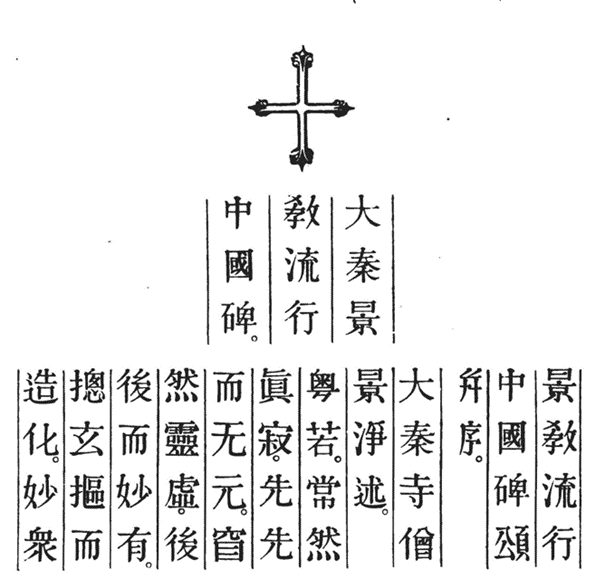
\includegraphics[width=\textwidth]{ChristologieCultureHistoire/Images/PremierParagrapheStele.png}
 
    \label{fig:my_label}
\end{figure}
 Si le livre d'Alopen 150 ans plutôt s'appelait simplement "Sûtra de Jésus-Messiah", le titre de la Stèle est le suivant :
\begin{quote}
    Monument rappelant la propagation à travers l'Empire du Milieu de l'Illustre Religion de Ta-ts'in. \cite{Havret:stelechretienne}
\end{quote}
Ta-ts'in (ou \emph{Da Qin}) indique l'Empire Gréco-Romain. Cette référence peut étonner quand on sait la répugnance des Eglises perses à être trop liées à Byzance. D'ailleurs, traditionnellement, le christianisme en Chine était appelé \textit{Bose Jiao}, l'\textit{enseignement Perse}.  En 745, il prend l'appellation officielle de religion de Da-Qin  possiblement par la chute de l'empire Sassanide perse un siècle plus tôt, qui rend caduque le terme de Perse, l'arrivée d'ambassades byzantines en Chine (attestée en 742) mais aussi par la référence à la philosophie grecque ainsi qu'à l'attribution de voyages en \textit{Da Qin} par le fondateur du Taoisme, Laozi :
\begin{quote}
    Calling Christianity the 'Religion of Da Qin' shows that the Nestorians of the Tang undeniably possessed a sensitive awareness of their political environment within China, and probably internationally as well, and moved with considerable acumen to secure the best possible position for themselves within it (\cite{Barrett:TaoismChristianity})
\end{quote}

\paragraph{Un découpage proposé en 25 sections} La stèle peut être découpée en 25 sections, la première sur les attributs de Dieu, puis les trois suivantes sur la Création et la Chute de l'homme (surtout pour développer l'idée d'un homme bon avant la chute par l'orgueil), puis les deux suivantes sur le Christ. A partir de la section 8, on trouve les caractéristiques de la religion, le baptême, les moines, l'éthique, puis plusieurs sections sur l'histoire des chrétiens en Chine, montrant une loyauté forte vis à vis des autorités politiques chinoises. Nous nous concentrerons sur les premières sections et en particulier les sections 6 et 7 proprement christologiques.  Il faut noter qu'une partie importante est liée à l'histoire du christianisme en Chine et la protection des empereurs. Cette attitude peut être mise en parallèle avec celle des premières communautés chrétiennes, avec Paul, montrant la compatibilité du christianisme avec l'Empire Romain (\cite{Baslez:MondeDevnuChretien}). 






\section{la partie proprement Christologique}

\subsection{Section 6 : l'incarnation} 

La première section qui nous intéresse parle de l'incarnation. Nous indiquerons à chaque fois les deux traductions en Français qui font foi (\cite{Havret:stelechretienne} et \cite{Pauthier:linscriptionSinganfou} \sn{la traduction de Havret est une traduction en latin et français mais la traduction française n'est pas complète - je l'ai complété à partir du texte latin}) :
 
\begin{tabular}{p{0.45\textwidth}p{0.45\textwidth}}
\\
Cependant, notre Trinité s'est comme multipliée, l'illustre et vénérable Messie, voilant et cachant son auguste majesté, se rendant tout semblable aux hommes, est venu en ce monde. les Puissances angéliques publièrent la bonne nouvelle; une femme vierge enfanta le Saint dans la grande Ts'in. Les esprits dans le Ciel annoncèrent la bonne nouvelle : "une Vierge a enfanté le Saint dans la grande Ts'in". Une étoile resplendissante a proclamé la faveur et la Perse, apercevant son éclat, vint lui faire hommage de ses présents. \cite[p. 35]{Havret:stelechretienne} & 

Ce faut alors que notre \textsc{Unité-trine} divisa sa personne dans le resplendissant et vénérable Messie, en voilant sa véritable majesté. il apparut dans le monde comme un simple mortel. Les Esprits dans le ciel annoncèrent la bonne nouvelle : "une Vierge a enfanté le Saint dans la Syrie !"  Une constellation resplendissante a proclamé l'heureux événement; les Perses ayant aperçu sa clarté, sont venus apporter leur tribut. \cite[p. 9]{Pauthier:linscriptionSinganfou} \\
                                                                                  
\end{tabular}
 
 \paragraph{Wo Sanyi, notre "trois-Un". } La pensée Taoiste utilisent le terme de Sanyi :  

\begin{quote} Le terme employé pour désigner la Trinité est un terme taoïste, \emph{sanyi} le "Trois-Un". mais pour signifier qu'il s'agissait de la Trinité Chrétienne, l'auteur de l'inscription a ajusté le caractère "\emph{Wo}" qui signifie "mon/notre". Ainsi le terme taoïste a pris un sens chrétien, "Notre Trois-Un".
    \cite[p.43]{Raguin:JesusMessieXian}
\end{quote}
Quelle est cette trinité taoïste ? Le Trois est pensé comme facteur d'harmonie entre l'Un et le Multiple permettant de «court-circuiter» la référence à Dieu ou à quelque instance supra-cosmique.\cite{Cheng:triadeChinoise}


Le terme utilisé pour le Christ est le terme syriaque de \textit{Messie}, translittéré et non traduit.

 "\textit{Voilant et cachant son auguste majesté, se rendant tout semblable aux hommes, est venu en ce monde}" est quasiment la traduction de Ph 2,6-7, soulignant l'abaissement du Christ.
 

\paragraph{Insistance sur le Ciel et l'environnement}  les cieux (\textit{constellation}) prennent une partie importante dans les deux sections sur le Christ, avec tout un passage sur l'Etoile des mages. On peut  déceler le souhait de l'auteur de montrer ce qu'est le Christ non pas en le décrivant directement comme \textit{forme},  causes ou \textit{logos} mais en insistant sur le \textit{fond},  \textit{le Ciel} qui \textit{ne s'exprime pas}. \cite[p. 109]{PolDroit:voyage} . 
\begin{quote}
    La philosophie gréco-européenne privilégie la « forme » – en grec ancien, \textit{eïdos}. Une « idée » est d’abord une « forme », qui se découpe sur un fond d’espace indifférencié. C’est ce fond d’espace qui retient l’attention chinoise, plutôt que la forme qui s’en détache. Scruter le fond plutôt que les formes, l’indifférencié plutôt que les différences, l’espace plutôt que les choses qui s’y trouvent et s’y découpent, telle pourrait être la première caractéristique de l’attitude chinoise.\cite[pp. 110-111]{PolDroit:voyage}  
\end{quote}
Dès lors, l'attitude des mages perses qui scrutent dans \textit{le Ciel} ce qui change, est finalement celle du sage Chinois. Pour le Taoisme, ce n'est pas par le discours, qui segmente et découpe mais par le biais d'histoires déroutantes, \textit{comme celle de l'étoile des mages}, que l'on peut transmettre la voie. \cite[p. 130-141]{PolDroit:voyage} 
 




\subsection{section 7 : la rédemption } 


Après l'incarnation, le texte développe en plusieurs paragraphes l'action de Jésus : 


\begin{tabular}{p{0.45\textwidth}p{0.45\textwidth}}
\\
Il accomplit les lois anciennes qu'avaient écrites les vingt-quatre Saints, direction des empires dans les conseils. Il fonda la nouvelle religion que la Trine unité, Esprit très pur, n'exprime pas au moyen de paroles, formant à la pratique des vertus par la vraie foi.  & Ainsi, s'est trouvé accompli ce que les vingt-quatre saints avaient annoncée dans l'ancienne loi : " le gouvernement des familles et des États par une grande et suprême doctrine. Il établit la doctrine pure de l'\textsc{unité-trine}, sans l'appeler une nouvelle religion. Il fortifia les bonnes habitudes par l'usage de la vraie foi. \\
\end{tabular}

\paragraph{Jésus est présenté comme un sage} Le texte insiste sur l'Esprit qui soutient la vertu sans passer par une loi (cf Jr 31,33 \sn{Jr 31,33 \textit{Je mettrai ma loi au dedans d'eux, Je l'écrirai dans leur coeur} \newline 2 Co 3,3\textit{Vous êtes manifestement une lettre de Christ, écrite, par notre ministère, non avec de l'encre, mais avec l'Esprit du Dieu vivant, non sur des tables de pierre, mais sur des tables de chair, sur les coeurs.}}  ou encore 2 Co 3,3).

Par cet  \textit{Esprit très pur, qui n'exprime pas au moyen de paroles formant à la pratique des vertus par la vraie foi}, l'auteur propose probablement une théologie accessible à la culture chinoise. pour les Chinois en effet,  ce n'est pas au moyen de raisonnements qu'on atteint le Ciel, qui s'éprouve directement
\cite[p. 117]{PolDroit:voyage} même si notre participation au Ciel en ce monde est parfois voilée.


Cependant, l'auteur ne s'arrête pas à une approche \textit{sans parole} puisqu'il mentionne les \textit{huit béatitudes} : 

\begin{tabular}{p{0.45\textwidth}p{0.45\textwidth}}
\\
Il institua les règles des huit fins, pour purifier les facultés et perfectionner les saints; il ouvrit la porte des trois principes,& Il posa les lois des huit limites morales que l'on ne doit point franchir. la poussière de la terre, purifiée comme le métal dans la fournaise, devint la vérité parfaite. Il enseigna au moindre les trois grandes vertus cardinales; 
\\ 
 en ouvrant les portes la vie et supprimant la mort. & il lui ouvrit les sources de la vie, et anéantit la mort.
\end{tabular}


 \paragraph{Référence à la Bible} Après avoir insisté sur l'éthique de Jésus, l'auteur met l'accent sur le corpus biblique, à la fois dans le registre de l'\textit{accomplissement} de l'Ancien Testament et ses 24 livres/ Saints mentionnés plus haut \sn{hors livres deutérocanoniques} que de l'annonce d'un nouveau Testament\sn{ l'auteur décompte 27 livres alors que le Corpus syriaque ne reconnaissait initialement que 22 livres (l'Apocalypse et les épîtres générales reconnus tardivement) }. 

 \paragraph{Sauver par le registre de la grâce} Face à poussière (Lieu-tch'en), expression bouddhique pour désigner les \textit{souillures de la pureté du coeur},  le texte mentionne les 8 lois morales (Pa-King, "8 circonstances"), comprises comme les Béatitudes (8 béatitudes chez Mt).  Sont aussi mentionnés la porte des trois vertus cardinales (Tch'ang), porte qui ouvre aussi à la vie et supprimant la mort (Mié-se) selon une expression chrétienne traditionnelle. 

Puis suit une expression typiquement bouddhique du soleil lumineux triomphant des porte des enfers (ti-yu) mot à mot \textit{prison de la terre} \cite[p. 49]{Havret:stelechretienne}.  Satan est ici appelé par le terme chinois \textit{Mo}, d'où la traduction de démon :

\begin{tabular}{p{0.45\textwidth}p{0.45\textwidth}}
\\
Il suspendit le soleil lumineux pour triompher de l'empire de ténèbres et {dès lors }les ruses du démons furent toutes pénétrées et déjouées
&  Il suspendit au ciel le brillant soleil de la vérité pour dissiper les habitations des ténèbres; les ruses mensongères du démon furent dès lors pénétrées et déjouées. \\
\end{tabular}



 
 
 

\begin{tabular}{p{0.45\textwidth}p{0.45\textwidth}}
\\
Conduisant à la rame la barque de la miséricorde, il s'éleva aux demeures lumineuses; dès lors quiconque possède une âme a trouvé son salut. L'oeuvre de la toute puissance étant ainsi consommée, il monta en plein midi, homme déifié.& Il mit en mouvement le navire de la miséricorde pour s'élever aux brillantes demeures; les âmes qu'il renfermait purent dès lors, en traversant le fleuve de la vie, obtenir cette fin glorieuse. A l'heure de midi, il s'éleva au séjour de la vérité. \\ Il laissait les vingt-sept livres de l'écriture, où est expliquée la grande réforme pour l'ouverture des \textit{ling-koan}
  \cite[p. 44]{Havret:stelechretienne} & 
Des saints livres ont été laissés au nombre de vingt-sept, qui ont étendu les conversions originelles en libérant les âmes.
  \cite[p. 10]{Pauthier:linscriptionSinganfou} \\
                                                                                  
\end{tabular}
 
  \paragraph{influence bouddhique du mouvement} Avec l'image de la barque de miséricorde (\emph{avalokites 'vara}), nous avons ici une belle image d'origine bouddhique, divinité plus connue en Chine sous le nom de \emph{Koan-yn} et surnommée \emph{Ta-t'se} la grande Miséricorde. D'après le bouddhisme, l'humanité tourne sans cesse comme sur une grande mer jusqu'à ce qu'elle arrive enfin au \textit{nirvana}. 
  
 % -----------------------------------------------
\section{Conséquences en terme de chemin de salut}

Quelles sont les conséquences sur le salut de cette étude rapide des deux paragraphes christologiques ?

\paragraph{Une dimension pratique du salut} Pour les chinois, la dimension pratique des débats est importante : 

\begin{quote}
    Entre ordre confucéen et contestation taoïste, il existe plus de complémentarité, malgré leurs désaccords, que d’opposition frontale. Ne perdant jamais de vue une dimension pratique, les débats chinois sont continûment traversés par des interrogations sur la bonté ou la méchanceté humaine, sur la bienveillance ou la cruauté nécessaire des souverains.

\cite[p. 147]{PolDroit:voyage}  
\end{quote}
 Regardons dans cet esprit le passage sur le mal qui précède les sections sur l'incarnation et la rédemption.
\begin{quote}
   Il arriva que Satan, disséminant ses fraudes, se para de l'ornement emprunté d'une pure essence, et qu'ouvrant une brèche dans cette grandeur morale, au milieu de cet heureux état, il y introduit la ressemblance de la confusion.
De là, des sectes aussi nombreuses que les jours de l'année, qui se suivirent pressées, et tracèrent à la suite leur sillon, tissant à l'envi les filets de leurs lois. les uns, désignant les créatures, s'appuyaient sur elles comme sur leur principe, les autres supprimant la réalité de l'Etre, se plongeaient dans la superstition, d'autres adressèrent des prières et des sacrifices pour attirer le bonheur, d'autres enfin firent parade de vertu pour en imposer aux hommes. 
\end{quote}
 
 
 Le péché introduit par Satan est décrit comme "ressemblance de la confusion". C'est un exemple de l'aspect concret du Chinois :\textit{ Tien-che }. \textit{Tien} signifie un ornement en métal; \textit{che}, chercher à paraître ce que l'on n'est pas ; se parer des dehors. La conséquence sont les \textit{sectes aussi nombreuses que les jours de l'année}; présentant les différentes voies de salut. On y a vu une critique du Taoisme (cette voie est accusé de diviniser les forces de la nature :  \textit{désignant les créatures, s'appuyaient sur elles comme leur principe}) et Bouddhisme aux tendances matérialistes et nihilistes (\textit{supprimant la réalité de l'Etre, se plongeaient dans la superstition}).  
 
 
 
 \paragraph{Par le Baptême, l'Esprit Saint nous éloigne des vaines gloires} Après la partie christologique, l'inscription développe les rites, d'abord le baptême, \textit{quittant les préoccupations vaines et mondaines pour obtenir la pureté}. Ce soucis d'humilité et de quitter le monde  rejoint la pensée du \textit{Chemin} ou \textit{Tao},  
 
 \begin{quote}
     à la fois faiblesse extrême (goutte d’eau) et puissance sans borne (océan). \ldots vent… C’est à force de faiblesse, si l’on ose dire, que le sage parvient à tant de puissance. 
\cite[p. 130 ]{PolDroit:voyage} 
 \end{quote}

Que ce soit dans la partie décrivant la chute ou au moment du baptême (et des vaines gloires), on trouve probablement une description adaptée aux oreilles chinoises, empreintes de la pensée Taoïste.

 Puis, l'auteur décrit la vie monastique : le rôle de la barbe et de la tonsure, images extérieures de la vie intérieure, l'absence d'esclave, l'égale considération de tout homme , le refus des richesses, la pratique de la générosité, le silence et la retenue. A ce titre, ils se présentent moins comme des moines bouddhiques que comme des sages pétris de sagesse confucéenne : 
 
 \begin{quote}
     Car le « mandat du Ciel », comme disent les confucéens, est présent avant tout dans le « sens de l’humanité » (ren) qui habite le cœur de chacun. Cette notion fondatrice, malaisée à définir, implique à fois, selon Confucius, d’être « juste dans le jugement », « conscient de la valeur de l’effort », « pacifique dans les conflits » et d’avoir de la « retenue ». Le \textit{ren} est ainsi l’instance de régulation des rapports entre les humains, agissant au cas par cas.

\cite[p. 122]{PolDroit:voyage}  
 \end{quote}
 Paul a préféré  l'aréopage au Temple, et les apologistes Chrétiens le terme néo-platonicien de  \textit{Logos} pour dire l'expérience du Christ et non les catégories des religions paiennes. De même, l'auteur de la \textit{Stèle} nous semble mettre en avant la sagesse confucéenne, plutôt que les moines Taoistes ou bouddhistes. Cette attention à la sagesse confucéenne explique peut être  la mention qui suit : les moines prient \textit{au secours des vivants et des défunts}, alors que la sagesse confucéenne accorde une importance forte au culte des ancêtres.
 
 

 
 
  
\paragraph{Ne pas penser séparément morale, rites privés et gestion des affaires communes} Une caractéristique importante de la civilisation chinoise est effet d’entrelacer doctrines morales, rites privés et gestion des affaires communes
\cite[p. 120]{PolDroit:voyage}. L'inscription développe non donc seulement le credo de la foi chrétienne (sections 7 et 8), mais aussi la morale et les rites (sections 9 et 10). A ces deux éléments s'ajoute la louange des empereurs chinois. Sur ce dernier point, les Chrétiens en Chine reprennent  la stratégie des chrétiens face à l'empire romain, qui s'inséraient dans le réseau de solidarité des villes par le rôle des évêques et des diacres (\cite{Baslez:MondeDevnuChretien}).


\section{Conclusion}

\paragraph{Une présentation du message Chrétien soulignant les aspects les plus accessibles à la pensée Chinoise} A travers l'étude de la Stèle, nous avons trouvé la présentation des principaux points de la Foi Chrétienne. Cependant, sans trahir le message chrétiens, l'auteur choisit une traduction qui résonne avec la culture chinoise. Au delà de la traduction, le choix des passages de la Bible comme \textit{l'Etoile dans le Ciel} ou l'accent sur certains points du rite comme la prière pour les défunts ou l'attention au \textit{Ren}, éclaire ce message chrétien de façon nouvelle. 
 
\paragraph{difficulté à penser l'acculturation religieuse} Dans nos recherches, nous avons rencontré des auteurs ne pouvant pas penser l'acculturation du message chrétien en dehors des catégories de l'hérésie. Ainsi, un article récent \cite{Gernet:Stele} s'oppose à l'interprétation d'une stèle de Xi'an acculturée à la culture chinoise et propose une clé de lecture basée sur un contexte de luttes théologiques internes au sein de l'Église nestorienne.

\begin{quote}
    rien ne prouve d'ailleurs clairement que les nestoriens aient songé à faire partager leurs croyances aux Chinois. [\ldots] Les circonstances et les mentalités étaient en effet tout à fait différentes de celle qui devait régner un millénaire plus tard, à l'époque de la contre-Réforme animée par une ambition de conquête universelle des esprits et des territoires (p. 245)
\end{quote}
Même si la communauté chrétienne qui a écrit la stèle était toujours fortement liée à l'Église perse - comme le montre les signatures de la stèle en araméen -, cette thèse nous parait difficilement acceptable à l'analyse. Les Eglises syriaques à cette époques nous sont certes assez mal connues; on peut noter l'importance du terreau judeo-chrétien à la création de ces Eglises, le milieu missionnaire parmi les marchands, la mixité culturelle, reflet des sociétés en monde iranien, la loyauté vis à vis des autorités politiques et le monachisme (\cite{Amir:CoranHistoriens}). Sans les relever tous, on retrouve de fait de nombreux éléments syriaque dans la Stèle (par exemple, influence des marchands et moines dans la création de l'Eglise de Chine), mais sans que cela ne remette en question le travail d'acculturation de la foi chrétienne en contexte chinois dont les marques sont soulignées par de nombreux sinologues. A tel point que c'est plutôt l'autre vision, celle d'une supposée trop grande acculturation qui est souvent soulignée (le P. Havret, sj note par exemple les 
\textit{    dangereux rapprochements} avec la culture Taoiste \cite[p.21]{Havret:stelechretienne}).   


Cette double polémique montre la difficulté à penser l'acculturation et sa conséquence en terme de christologie : notre vision du Christ est forcément transformée par l'acculturation, et elle peut être vécue sans être un dévoiement de la foi véritable, mais au contraire en développant des aspects du Christ qui sont restés comme en germe dans son incarnation en Judée "au temps d'Hérode" et qui peuvent se développer pleinement dans d'autres cultures et époques. 



%
\subsubsection{1.1.2 les thématiques des versets
médinois
}

- le thème d'Abraham comme «~Père des croyants~» où Abraham est dit
d'une part \emph{ḥanīf}, c'est-à-dire monothéiste exclusif, mais aussi
\emph{muslim}, c'est-à-dire soumis, abandonné à Dieu, et ni juif ni
chrétien, date de la période médinoise.

(S. 3, 67-68).

«~Abraham n'était ni juif ni chrétien, mais il était un monothéiste
exclusif, abandonné à Dieu~; il n'était pas au nombre des polythéistes.
Les hommes les plus proches d'Abraham sont vraiment ceux qui l'ont
suivi, ainsi que ce Prophète et ceux qui ont cru~».
\marginpar{ \footnotesize This is a margin note using the geometry package, set at 5cm 
vertical offset to the first line it is typeset.}


\foreignlanguage{arabic}{لَكِنْ
}
test
\TArabe{مَا كَانَ إِبْرَاهِيمُ يَهُودِيًّا وَلَا نَصْرَانِيًّا وَلَكِنْ
كَانَ حَنِيفًا مُسْلِمًا وَمَا كَانَ مِنَ الْمُشْرِكِينَ إِنَّ أَوْلَى
النَّاسِ بِإِبْرَاهِيمَ لَلَّذِينَ اتَّبَعُوهُ وَهَذَا النَّبِيُّ
وَالَّذِينَ آَمَنُوا وَاللَّهُ وَلِيُّ الْمُؤْمِنِينَ}




\begin{otherlanguage}{arabic}
{مَا كَانَ إِبْرَاهِيمُ يَهُودِيًّا وَلَا نَصْرَانِيًّا وَلَكِنْ
كَانَ حَنِيفًا مُسْلِمًا وَمَا كَانَ مِنَ الْمُشْرِكِينَ إِنَّ أَوْلَى
النَّاسِ بِإِبْرَاهِيمَ لَلَّذِينَ اتَّبَعُوهُ وَهَذَا النَّبِيُّ
وَالَّذِينَ آَمَنُوا وَاللَّهُ وَلِيُّ الْمُؤْمِنِينَ}
\end{otherlanguage}

Ce verset a bien sûr donné lieu à de multiples commentaires. Il est
souvent interprété dans le sens où Abraham est dépositaire de la
religion originelle avant son altération par les juifs et les chrétiens. \cite{Ben62}
Souvent ne veut pas pour autant dire toujours. Il y a d'autres
lectures\ldots{} \sn{\cite{Ben62}}

\begin{figure}
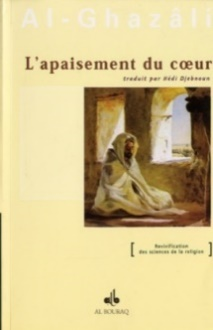
\includegraphics{Images/image002.jpg}
\sidecaption{essai}
\end{figure}


\begin{table}[h!]
\resizebox{\textwidth}{!}{%
\small
\begin{tabular}{p{2cm}p{4cm}p{4cm}}
\toprule
essai & essai & essai \\
\midrule
essai & essai & essai \\
\bottomrule

\end{tabular}%
}
\sidecaption{essai}
\end{table}

\begin{longtable}{p{6cm}p{6cm}}
\toprule
\endhead
«~Quiconque obéit au Messager obéit certainement à Allah~». 
&\TArabe{ مَّن
يُطِعِ الرَّسُولَ فَقَدْ أَطَاعَ اللَّهَ }\\
\bottomrule
\end{longtable}
%\part{Sacramentaire}



\chapter{Introduction}
%---------------------------------------------------------------------------------------------------------------

\mn{LM Chauvet}

\hypertarget{pour-se-repuxe9rer-dans-le-vaste-monde-de-la-sacramentalituxe9-lorganisme-sacramentel}{%
\section{Pour se repérer dans le vaste monde de la sacramentalité~:
l'organisme
sacramentel}\label{pour-se-repuxe9rer-dans-le-vaste-monde-de-la-sacramentalituxe9-lorganisme-sacramentel}}

\hypertarget{sacrement-un-concept-analogique}{%
\paragraph{«~Sacrement~»~: un concept
analogique}\label{sacrement-un-concept-analogique}}

\hypertarget{lorganisme-sacramentel-analyse-systuxe9mique}{%
\paragraph{l'organisme sacramentel~: analyse
systémique}\label{lorganisme-sacramentel-analyse-systuxe9mique}}

\hypertarget{une-duxe9finition-des-sacrements}{%
\paragraph{\texorpdfstring{Une définition des
sacrements}{ Une définition des sacrements}}\label{une-duxe9finition-des-sacrements}}
 

%---------------------------------------------------------------------------------------------------------------
\section{Ouverture sur la problématique
d'ensemble} 

la pointe des sacrements~: la communication de Dieu, la grâce.

«~\textbf{pour la Gloire de Dieu et le salut du monde~»}

dimension latreutique dimension sanctificatrice

Nos liturgies exercent de multiples fonctions~: cognitives, philo,
économiques~!, sociales\ldots{} quei ne doivent pas masquer
l'essentiel~: \textbf{la communication de Dieu.}

\begin{Ex}
 «~le Corps du Christ~: Amen~»

\begin{itemize}
\item
  on ne peut pas faire plus bref
\item
  de la foi
\item
  ie~: les mots «~nus
\end{itemize}

Cette nudité des mots qui se visibilise par la nudité de la main tendue,
\textbf{nue.}
\end{Ex}


Le salut de Dieu , dit dans la Parole, vient se déposer sur le corps.

Pb~: Comprendre ce que l'on célèbre~: «~Lex orendi, lex credendi~».

\paragraph{3 modèles de compréhension~:}

\hypertarget{moduxe8le-objectiviste}{%
\paragraph{Modèle objectiviste}\label{moduxe8le-objectiviste}}

St Thomas d'Aquin -\textgreater{} Trente -\textgreater{} Catéchisme de
1947\sn{«~des signes sensibles institués par Notre Seigneur Jésus
  Christ pour produire ou augmenter la grâce dans nos âmes~».}

\textbf{Sacrement comme instrument de production de la grâce~;
insistance sur la dimension de «~cause~» ou de moyen du salut.}

Dieu -\textgreater{} Sacrement -\textgreater{} Homme -\textgreater Dieu

Pb~: l'homme n'intervient pas dans le sacrement

\begin{itemize}
\item
  peu importe que l'homme «~comprenne~», pourvu qu'il soit sanctifié =
  limite)
\end{itemize}

Insistance~: Sacrement comme moyen, cause de salut

Avantage~: \textbf{souligne l'action de Dieu.}

\textbf{Instrument, canal, remède, germe.}

\hypertarget{moduxe8le-subjectiviste}{%
\paragraph{Modèle subjectiviste}\label{moduxe8le-subjectiviste}}

En réaction

Cf K. barth, qui craignait que la Liberté de Dieu soit «~compromise~»
par les sacrements, trop canalisée.

Le Baptême ne fait que \textbf{refléter} la \emph{justification et la
sanctification.} Dieu l'a déjà fait.

Contre une conception~»magique~» des sacrements.

Dieu -\textgreater{} Homme --\textgreater{} Sacrement -\textgreater{}
Dieu

\textbf{Sacrement comme instrument de traduction du déjà-là de la grâce.
Insistance sur la dimension de «~signe~» de salut (déjà donné).}

Avantage~: prend bien en compte le vécu humain. Dieu n'a jamais été lié
par les sacrements dans sa puissance de salut.

Inconvénient~: ne rend pas compte de l'efficacité du sacrement
lui-même.~: Trop exclusif.

Mais ce schéma va contre toute la \textbf{Tradition Chrétienne }(y
compris les pères).

Il est pourtant très à la mode, en réaction contre l'Église et en
insistant sur l'orthopraxie au lieu de l'orthodoxie.

\hypertarget{moduxe8le-vatican-ii}{%
\paragraph{Modèle Vatican II}\label{moduxe8le-vatican-ii}}

Schéma à «~double sens~»

Essai de tenir ensemble les dens sens (moyen de salut et signe du salut)

Dieu $\leftarrow$ $\rightarrow$ Homme $\leftarrow$ $\rightarrow$ Sacrement $\leftarrow$ $\rightarrow$ Dieu

Dieu~: \textbf{sujet opérateur des sacrements (}moyen de
salut-\textgreater{} vie humaine sanctifiée = louange à Dieu)

Difficulté~: tenir bien ensemble les deux sens

«~signe~» et «~cause~» ne sont pas des \textbf{catégories homogènes}


\paragraph{Question d'ouverture}

St Thomas d'Aquin~: II a II ae 89 prologue~; question sur l'éthique

→ on pourrait traiter ici (éthique) des sacrements → \textbf{sommet de
la vie éthique}

il aurait pu dire~: «~cause signifiante~» ou signe «~causant~».

un signe qui ne signifie que par mode de cause

une cause qui ne cause que par mode de signe

Chauvet, «~symbole et sacrement~»

Cf langage

\emph{Alliage homogène entre les deux~; grâce aux outils concernant le
\textbf{langage. }}

«~signe efficace~»~: mais c'est comme le langage~!

%-------------------------------------------------------------------------------------------------------------------------------
\section{Sacrement~: approche historique}

%-------------------------------------------------------------------------------------------------------------------------------
 
La constitution de la sacramentaire

Article LM Chauvet, «~sacrements~» dans Catholicisme

\hypertarget{mysterion-sacramentum}{%
\subsection{Mysterion -- Sacramentum}\label{mysterion-sacramentum}}

méfiance initiale contre le mot~; utilisé par les religions à mystère.

\textbf{Tertullien~;} aspect juridique~: la caution, le serment (cf
renonciation au mal)

Le Baptême comme \emph{pacte (foedus).}

La traduction en latin a fait perdre le lien avec le mysterion biblique,
l'économie divine.

Un vécu liturgique essentiel

\hypertarget{la-contreverse-sur-le-baptuxeame-des-huxe9ruxe9tiques}{%
\subsection{La contreverse sur le Baptême des
hérétiques}\label{la-contreverse-sur-le-baptuxeame-des-huxe9ruxe9tiques}}

Cyprien → Baptême lié à l'Église donc si deux Églises, deux Baptêmes .

→ Donatiste

en face Augustin~:~»le Christ agit «~etiam per malum ministrum~».

mais réception elle est fonction des dispositions personnelles.

\hypertarget{le-haut-moyen-uxe2ge}{%
\subsection{Le Haut moyen-âge}\label{le-haut-moyen-uxe2ge}}

présence réelle~: première question

\hypertarget{la-scholastique}{%
\subsection{la scholastique}\label{la-scholastique}}

la théologie comme science.

D'abord la finalité puis Importance de la causalité (Airstote)

Pratique de la LOI~: signifiait le Foi qui sauve mais ne causait pas le
salut. Signe non causal.

Importance de la pratique

Limites~:

\begin{itemize}
\item
  un schéma fondamentalement «~productionniste~»
\item
  le Cloisonnement des sept sacrements (et non les sacrements liés BEC
  cf 44)
\item
  l'absence d'ecclésiologie entre la christologie et la sacramentaire
\item
  une théologie trop en marhe de l'action liturgique
\item
\end{itemize}

\hypertarget{ouverture}{%
\section{ouverture}\label{ouverture}}

la sacramentaire scolastique est le fruit de la nouvelle
«~\emph{epistemé~»} né au 12° siècle . La fidélité à la grande tradition
théologique nous requiert non pas de reproduire mais d'en faire une
hérméneutique (décodage/recodage) nécessairement nouvelle ou sein de la
nouvelle culture qui est la notre.

 
%-------------------------------------------------------------------------------------------------------------------------------
\chapter{Sacrement de la Réconciliation}

%-------------------------------------------------------------------------------------------------------------------------------

Le «~Sacramentum~» comme langage symbolique et rituel

\hypertarget{introduction}{%
\section{Introduction}\label{introduction}}

Trilogie d'inspiration agustinienne~:

\begin{itemize}
\item
  \textbf{sacramentum -- rite- célébration --} ce qui se voit
\item
  \textbf{res sacramenti -- réalité du sacrement = la grâce}
\item
  \textbf{res et sacramentum~: 1\textsuperscript{er} effet de la grâce,}
  qui n'est pas la grâce finale ou \textbf{caractère~:}
\item
   
  ex~: on peut «~perdre~» la res sacrementi du Baptême tout en
  conservant la \emph{res et sacramentum.} (on reste baptisé).
   
\end{itemize}

Sacramentum → res sacramenti

\emph{res et sacramentum~}comme frontière

Entre le signe humain →

→ \textbf{médiation} ecclésiale ou 1\textsuperscript{ère} effet

Et la grâce de Dieu →

 %---------------------------------------------------------------------------------------
  \section{Problématique du langage} 

\begin{Synthesis}
    \begin{enumerate}
  \item
    {La langage n'est pas un instrument à la disposition de
    l'homme~; il est la médiation d'avènement du sujet c'est à dire le
    milieu dans lequel advient le sujet}
  \item
    {Puisqu'il n'est jamais de sujet hors langage (ou hors
    culture), constamment nous parlons ou «~ça parle~» en nous} \sn{Exemple~: culture où il n'y a qu'un seul mot «~s'occuper~» pour
      dire \emph{travailler} ou \emph{avoir des loisirs.} Le plus
      naturel , chez nous, est souvent le plus culturel.}

 
  \item
    {D'où la révolution épistémologique contemporaine quant à la
    manière de comprendre le rapport entre le sujet et le réel}
  \end{enumerate}
\end{Synthesis}


\textbf{Sujet} $\leftarrow$ $\rightarrow$ \textbf{Réel}

→ \emph{perception du}

\emph{← image mentale~; concept}

\begin{itemize}
\item
  \emph{restitution}
\end{itemize}

Langage

Pb de ce schéma~: il pose le langage comme instrument~: sujet =
antérieur (logiquement) au langage


\begin{Prop}
    {le concept d'~"expression" dans cette perspective~: le
  langage est simultanément «~révélateur~» et «~opérateur~»}
\end{Prop}



\textbf{Sujet} $\leftarrow$ $\rightarrow$ \textbf{Réel}

\textbf{Langage - culture}

{$\rightarrow$ \textit{le rapport au réel est toujours déjà aménagé~;} il est toujours
construit (le découpage sémantique n'est pas le même selon les cultures)
\textbf{le réel construit comme monde}}

\emph{$\leftarrow$le sujet se construit ainsi comme sujet}

Transition~:

Fonction du langage~: pas seulement utilitaire (information) mais
dimension symbolique (communication)

\hypertarget{probluxe9matique-du-symbole}{%
\section{Problématique du symbole}\label{probluxe9matique-du-symbole}}

\hypertarget{le-symbole}{%
\subsection{Le symbole}\label{le-symbole}}

Le symbole est médiateur de reconnaissance et d'alliance entre les
sujets.\sn{Cf Tertullien~; \emph{militia Christi}}

 
\paragraph{Le symbole antique}
 

Cf Tobie, 5 «~quel signe de reconnaissance donnerai-je~?~»

Triple aspect~:

\begin{itemize}
\item
  Systémique~: 1 élément n'est symbole que dans son rapport avec les
  autres éléments du même ensemble
\item
  Identitiaire~: se reconnaître comme partenaire
\item
  Juridique~: il faut être d'accor sur les \textbf{règles du jeu~.}
  Instance tierce de la Tradition, de la Loi~?
\end{itemize}
\mn{Cours du 4/2/03

Cours du //03}


Echange symbolique~: hors valeur

Intérêt théologique, grâce et échange symbolique

\hypertarget{luxe9change-symbolique}{%
\subsection{2.3 L'échange symbolique}\label{luxe9change-symbolique}}

\hypertarget{intuxe9ruxeat-thuxe9ologique}{%
\paragraph{2.32 Intérêt
théologique}\label{intuxe9ruxeat-thuxe9ologique}}

\hypertarget{b.-parole}{%
\paragraph{b. Parole}\label{b.-parole}}

Il n'y a rien de plus efficace que la parole

La parole ce n'est pas que des mots

Il suffit d'un «~je t'aime~» pour que la vie revienne

Mais aussi à travers le corps

\hypertarget{ruxe9flexion-sur-leucharistie}{%
\subparagraph{Réflexion sur
l'eucharistie}\label{ruxe9flexion-sur-leucharistie}}

Jn 6~: Pain de vie

Jésus est le pain de vie descendu du ciel

Rapport à la \emph{manne.}

\begin{itemize}
\item
  Mannu~: qu'est ce que c'est~?
\item
  On ne peut pas la stocker (ce n'est pas de la valeur)
\item
  Elle est donné quotidiennement
\item
  Sg 16~: «~elle était comme le pain des anges et elle s'adaptait au
  goût de chacun) Sg C'est vraiment du miel qu'est la sagesse
\item
  Beauchamp~: \emph{c'est le pur signe non chose}
\end{itemize}

La manne se prétait particulièrement à une analogie de la PAROLE.

1\textsuperscript{ère} tentation de la faim~: Mt 4,4 l'homme ne vit pas
seulement de pain mais de la parole qui sort de la bouche de Dieu.

\begin{itemize}
\item
  Dieu donne la manne pour que l'homme comprenne que la parole fait
  vivre (ref à Dt 8~?)
\item
  Pour manger l'eucharistie, il faut avoir ruminer la parole (cf
  élévation de la Bible et élévation de l'eucharistie)
\item
  Christ se présente comme la parole de vie envoyé par Dieu. Jn comprend
  la manducation d'eucharistie est une rumination de la parole douce et
  amère d'un Christ qui se livre pour la vie du monde.
\end{itemize}

L'expérience anthropologique de manger physiquement la parole pour
qu'elle soit complétement entendu~: d'où l'eucharistie~: parole donnée
sous le mode sacramentel

La Parole, c'est le Christ

\begin{itemize}
\item
  2 Co 10~: Le Christ est le OUI de Dieu au monde.
\end{itemize}

\hypertarget{eviter-le-piuxe8ge-de-la-chosification}{%
\subparagraph{Eviter le piège de la
chosification}\label{eviter-le-piuxe8ge-de-la-chosification}}

L'échange symbolique permet de ne pas chosifier ni magnifier (S Thomas
n'avait pas cet outil conceptuel~: dommage~!)

\hypertarget{c.-gratuituxe9}{%
\paragraph{Gratuité}\label{c.-gratuituxe9}}

\textbf{Charis}~: la grâce, ce qui est gratuit

Deux sens~:

\begin{itemize}
\item
  gratis Data~: donné gratuitement
\item
  \emph{gratiam gratum~:} gracieuseté. celle qui nous rend gracieux aux
  yeux de Dieu. Père de l'Eglise.
\end{itemize}

D'une part la grâce est gratuite~: elle ne dépend pas de nos mérites.

MAIS cela ne veut pas dire qu'il n'y ait pas de CONTRE DON, car sinon,
Dieu nous traiterait comme un OBJET (ALIENATION~: nous serions alors
écrasés). Or, il nous traite comme un SUJET. \emph{Un DON oblige.} Ce
n'est pas la \emph{conséquence} mais la \emph{marque} du don, car sinon
ce n'est pas un don car il n'est pas reconnu par la personne qui le
reçoit.

DON RECEPTION CONTRE-DON

Quand nous rendons grâce à Dieu pour les dons, nous ne sommes pas dans
le marchandage.

\hypertarget{baptuxeame-des-petits-enfants}{%
\subparagraph{Baptême des petits
enfants}\label{baptuxeame-des-petits-enfants}}

Le plus bel exemple de la gratuité de la grâce~: il ne tient pas compte
des mérites et démérites pour nous sauver. Mais il renforce un schème de
concurrence entre Dieu et l'Homme. Car le contre-don n'est pas marqué.
D'où l'importance de penser le baptême des petits enfants comme un
dérivé des adultes~: ACTE LIBRE~; êtres responsables.

\hypertarget{d.-le-thuxe9ologal-dans-lanthropologique}{%
\paragraph{le théologal dans
l'anthropologique}\label{d.-le-thuxe9ologal-dans-lanthropologique}}

échange symbolique pour approcher le mystère de la rencontre entre Dieu
et l'homme dans les Sacrements (leur efficacité)

\begin{itemize}
\item
  pas une simple analogie~: c'est la STRUCTURE dans laquelle s'effectue
  cette échange
\item
  le théologal se joue dans l'anthropologal, dans la constitution de
  l'homme
\end{itemize}

\hypertarget{lacte-de-symbolisation-analyse-et-application-uxe0-leucharistie}{%
\subsection{L'acte de symbolisation~: analyse et application à
l'eucharistie}\label{lacte-de-symbolisation-analyse-et-application-uxe0-leucharistie}}

2 agents secrets, avec billet de banque~déchiré; acte de symbolisation
pour se reconnaître partenaire

caractéristique

\begin{itemize}
\item
  systémique
\item
  symbolique
\item
  juridique (il faut avoir défini préalablement que le billet était le
  code de rencontre)
\end{itemize}

 

\begin{table}[h!]
    \centering
    \sidecaption{articuler  }
 
\begin{tabular}{p{.2\textwidth}p{.2\textwidth}p{.2\textwidth}}
\toprule
Christ &$\leftarrow$ $\rightarrow$ & Eglise \\
 
\\
\bottomrule
\end{tabular}
\label{tab:my_label}
\end{table}

 

 
\begin{table}[h!]
    \centering
\sidecaption{Des éléments du même ensemble mais qui sont
différents  }
 
\begin{tabular}{p{.2\textwidth}p{.2\textwidth}p{.2\textwidth}}
\toprule
Christ &($\leftarrow$ $\rightarrow$) & Eglise \\
 
\\
\bottomrule
\end{tabular}
\label{tab:my_label}
\end{table}


 

Ex~: un signe de Croix chez les papous~: ils ne peuvent pas le rattacher
aux autres éléments~: FONCTIONNEMENT imaginaire

\begin{table}[h!]
    \centering
\sidecaption{Chaque élément ne tient sa pertinence symbolique que de
par le rapport qu'il entretient avec les autres éléments de
l'ensemble
Le Christ n'existe que par l'Eglise dans le sens que sans Eglise,
personne ne connaîtrait le Christ }
\begin{tabular}{p{.2\textwidth}p{.2\textwidth}p{.2\textwidth}}
\toprule
Christ &$\leftarrow$& Eglise \\
        &   $\rightarrow$ \\
\\
\bottomrule
\end{tabular}
\label{tab:my_label}
\end{table}


\hypertarget{eucharistie}{%
\subparagraph{Eucharistie}\label{eucharistie}}

1Co 11~: Paul reproche au Co de prendre le repas du Seigneur

\begin{enumerate}
\def\labelenumi{\arabic{enumi}.}
\item
  niveau \emph{ecclésiologique et Ethique}~: vous prétendez prendre le
  repas alors que votrer pratique est en contradiction
\item
  niveau sacramentaire~ ou plutôt liturgique : Paul raconte le récit de
  la cène~: iatus entre la réponse et le problème posé
\item
  donc «~discernez le corps~». Le problème des Co, ce n'est pas la
  transsubstantiation\sn{Question apparue au IXème\ldots{}} (pas
  un problème sur la présence réélle). Mais mettre en rapport les
  membres du corps du Christ avec le corps Sacramentel (1 et 2)
\end{enumerate}

\hypertarget{rite-de-communion}{%
\subparagraph{Rite de Communion}\label{rite-de-communion}}

Lex Orandi, Lex Credendi

Regarder comment se pratique la célébration

\begin{table}[h!]
    \centering
      \sidecaption{ }
 
\begin{tabular}{p{.2\textwidth}p{.4\textwidth}}
\toprule
Geste de paix & «~Donnez-vous la paix~»~: ce qui est premier, c'est le
rapport horizontal avec mes frères \\
Fraction de paix & Rapport vertical (le Christ) pour faire l'unité des
membres de son corps (horizontal) \\
Démarche de Communion & Rapport vertical \\
\\
\bottomrule
\end{tabular}
\label{tab:my_label}
\end{table}
 

On ne peut pas séparer l'Eglise du Christ

\hypertarget{huxe9ruxe9sie-de-buxe9renger-de-tours}{%
\subparagraph{Hérésie de Bérenger de
Tours}\label{huxe9ruxe9sie-de-buxe9renger-de-tours}}

XIème 1053

Hérésie sur la présence du Christ dans l'eucharistie

Pb~: on n'a pas les outils conceptuels pour penser cette présence du
Christ. On pensait une adhérence du Christ aux espèces, qu'on aurait dû
le voir. Seulement par un deuxième miracle, Dieu étant un voile qui nous
le cache, afin que nous fassions un acte de foi (Isidore de Seville).

Il a fallu attendre le XII, pour que l'on trouve le concept adéquat,
celui de SUBSTANCE aristotélicien (on ne voit que les Accidents).

Les trois corps sont liés~:

\begin{enumerate}
\def\labelenumi{\arabic{enumi}.}
\item
  Corps historique et glorieux
\item
  Corps mystique sacramentel
\item
  Corps écclésial
\end{enumerate}

2---3~: Soyez ce que vous voyez~; recevez ce que vous êtes. Aug.
\sn{A lire sur S. Augustin~: Chair\ldots, Chair de l'Eglise Tillard}

Corpus Verum~était devenu le Corps ecclésial (H. de Lubac). Mais
berenger diminue le lien entre 1 et 2. En réaction, on a renforcé 1 et 2
au détriment de 2 et 3. L'adoration du Christ dans l'Eucharistie est
devenue plus importante que la Communion.\sn{\textbf{Historique}~:

  Pratique de la communion annuelle

  La réserve eucharistique (pour les malades) se formalise

  Evolution d'une conception de l'eucharistie action vers l'eucharistie
  chose (ex~: Transubstanciation en réaction contre l'hérésie de
  bérenger de Tours, qui utilise le concept aristotélicien de substance
  XII).

  Développement des processions, XIII «~le peuple n'a plus faim du pain
  eucharistique, rassasié des processions~».

  Elévation~: telle importance que l'on en attend de merveilleux effets
  deprotection contre les malheurs ou de vision miraculeuse du Christ
  lui même
  Exposition du Saint Sacrement dans une monstance lors de la
  contre-réforme}

\hypertarget{quimporte-la-valeur-de-luxe9luxe9ment-symbolique}{%
\paragraph{Qu'importe la valeur de l'élément
symbolique}\label{quimporte-la-valeur-de-luxe9luxe9ment-symbolique}}

Le symbole ne fonctionne pas à la valeur~: Crucifix~: bout de bois~;
bague de fiançailles

Musique~: ky-ri-e suffit -- pas besoin de 10 Mn de kyrie de
Mozart\ldots{}

\hypertarget{le-laboureur-et-ses-enfants-de-la-fontaine}{%
\subparagraph{«~Le laboureur et ses enfants~» de la
Fontaine}\label{le-laboureur-et-ses-enfants-de-la-fontaine}}

\begin{itemize}
\item
  Gardez-vous de vendre l'héritage, il y a un grand trésor dedans
\item
  ils labourent le champ
\item
  le travail est le trésor
\end{itemize}

Analogie intéressante avec le sacrement~:

\begin{itemize}
\item
  le sacrement n'est pas un trésor dans le champ
\item
  J'en suis obligé Grammaticalement~: la grâce est posé comme Objet
\item
  SUJET -- VERBE -- OBJET~: Dieu Donne la Grâce
\item
  Penser en théologie comme en philosophie, c'est apprendre à se défaire
  de son discours.
\item
  Heiddegger casse le langage~; Lévinas. Contre réduction
  phénoménologique. Risque certes de préciosité. Mais il faut casser les
  représentations.
\item
  La grâce n'est pas un objet valeur, même spirituel
\item
\item
  nous sommes la terre labourée. DurchArbeitung de Freud~: nous sommes
  travaillés
\item
  le socle de la charrue, c'est la parole de Dieu qui nous advient sous
  le mode rituel
\item
  il faut une force de traction, c'est l'ES
\item
  Nous allons nous transformer en acteur d'Alliance, alors que nous
  sommes tous héritier de Cain.
\item
  Cet engendrement permanent de nous même, nous devenons un peu plus
  fils de Dieu.
\end{itemize}

\begin{Def}[Grâce]
 un «~se recevoir~» toujours en cours
\end{Def}
  

\hypertarget{lacte-de-symbolisation-est-simultanuxe9ment-ruxe9vuxe9lateur-et-opuxe9rateur}{%
\paragraph{L'acte de symbolisation est simultanément révélateur et
«~opérateur~»}\label{lacte-de-symbolisation-est-simultanuxe9ment-ruxe9vuxe9lateur-et-opuxe9rateur}}

Le billet est à la fois «~révélateur~»~: ils se reconnaissent équipiers
mais aussi «~opérateur~»~: ils sont liés jusqu'à la mort dans leur
projet.

\hypertarget{doxologie}{%
\subparagraph{Doxologie}\label{doxologie}}

Par lui, avec lui et en lui

On présente à dieu , conjoint la terre au Ciel.

La voix monte aussi vers Dieu ainsi que les bras. Mais ce que nous
montons, c'est le Christ.

Puissance incroyable

Le Chrétien~: se reconnaît à Dieu, pour Dieu, en Christ.

C'est à force de faire des gestes comme cela que l'on devient Chrétien
et de les faire en Eglise. Attention à ne pas le psychologiser.

Une Foi ne vit qu'en se MANIFESTANT. Si on ne le dit jamais, notre foi
est quasiment morte.

\hypertarget{quelques-lois-de-la-ritualituxe9}{%
\section{Quelques lois de la
ritualité}\label{quelques-lois-de-la-ritualituxe9}}

\hypertarget{un-jeu-de-langage-original}{%
\subsection{Un «~jeu de langage~»
original}\label{un-jeu-de-langage-original}}

Ex~: génocide du Rwanda

\begin{itemize}
\item
  type \textbf{exactitude}~: discours du politologue
\item
  type témoignage~: discours du témoin~: reconstruit l'évenement pour ce
  faire comprendre. \textbf{Vérité narrative ou herméneutique}
\item
  type poétique~: vérité \textbf{poétique.} On ouvre un monde possible
  (Ricoeur)
\item
  Les trois types de langages visent la vérité de différentes voies.
\end{itemize}

Différents langages de ritualité~:

\begin{itemize}
\item
  théologique
\item
  mystique~: métaphore, affects (S. jean de La Croix)
\item
  témoignage~: MCC. On se raconte.
\item
  rituel
\end{itemize}

Attention, à ne pas se tromper de registres~: respecter les jeux de
langage différents. Ex~: à la messe, on ne parle pas de la théologie du
péché originel.

La liturgie croule sur les demandes contradictoires. Elle est faite pour
que l'on puisse recevoir le don de Dieu. Elle ne permet pas tout.

\hypertarget{lecture-thuxe9ologique-de-quelques-caractuxe9ristiques-majeures-de-lexpression-rituelle}{%
\subsection{Lecture théologique de quelques caractéristiques
majeures de l'expression
rituelle}\label{lecture-thuxe9ologique-de-quelques-caractuxe9ristiques-majeures-de-lexpression-rituelle}}

\hypertarget{un-langage-pragmatique-langage-action}{%
\paragraph{3.21 Un langage pragmatique~: langage
--action}\label{un-langage-pragmatique-langage-action}}

c'est une «~URGIE~» - ergon~: action\sn{Siderurgie,
  chirurgie,\ldots{}}

de l'ordre de la communication symbolique. Ne s'indresse pas à
l'intellect (non pas un LOGOS\sn{théologie,}) mais à tout le
corps. Lieu de jouissance~: on a une rencontre avec le Dieu Bon (et non
pas le Dieu Vrai\ldots).

\begin{itemize}
\item
  mon âme a soif de Dieu
\end{itemize}

\hypertarget{cuxe9luxe9bration-pour-les-enfants}{%
\subparagraph{Célébration pour les
enfants}\label{cuxe9luxe9bration-pour-les-enfants}}

But~: leur laisser 5 mn avec Dieu

\hypertarget{cest-la-muxe9moire}{%
\subparagraph{C'est la mémoire}\label{cest-la-muxe9moire}}

La liturgie, c'est une mémoire~: les places sont en attente\ldots{} Même
les gestes,

La faiblesse de Croire, Michel de Certeau

\textbf{Faites ce que vous dites~}: ex~: soyez dans la joie = chanter.
Ex~: onction au Baptême~: pas besoin d'expliquer~: cela sent bon,
imprègne le front.

\mn{Cours du 7/03/02}

\hypertarget{petite-lecture-thuxe9ologique}{%
\paragraph{Petite lecture
théologique}\label{petite-lecture-thuxe9ologique}}

Notion de \textbf{parole}~: sens d'Action en hebreu

\begin{itemize}
\item
  pas le logos grec
\item
  le DABAR (traduire par  dans la LXX)
\item
  SACREMENT, déploiement de ce qu'est le DABAR, la parole
\end{itemize}



    \paragraph{Un langage symbolique, donc économique~: sobriété et
    «~réserve~» du
    rite}

Symbole~: il rend PRESENT la chose (cf le drapeau brulé)~: il EST et il
n'EST pas le réel qu'il représente.

Les symboles représentent des mondes

Le symbole est \textbf{sobre.} Un peu suffit. Ex~: \emph{donnons-nous un
signe de paix~: ainsi nous nous engageons à nous réconcilier~; pas
besoin de faire le tour de l'Eglise.} Un peu de vin, un peu d'eau. Il ne
faut jamais substituer le réel au symbole.

Donner la chance au symbole~: ne pas tout expliquer~: on s'est trompé de
registre.

Goupillon~: moyen age~: préférer du buis.

Attention à la dérive \textbf{festive.} Injonction~: «~quand il
\emph{faut} faire la fête, ce n'est pas drôle\ldots~». Elle peut surtout
faire obstacle au passage de la mort vers la vie à faire avec le Christ.

Geneviève Hébert, Eloge \emph{de la pudeur en matière de dévotion et
ailleurs}, MD 215-225

LM Chauvet, \emph{Eschatologie et Sacrement}, MD 220\\
nos symboles liturgiques sont sobres. Elle est la médiation de la
condition eschatologique dans laquelle nous sommes~: le salut est déjà
donné mais pas encore achevé. Nous chantons «~\emph{Alleluia}~» car déjà
là mais nous ne nous laissons pas entraîner car tout n'est pas déjà
acquis~: cela peut être une insulte à tous les gens qui souffrent depuis
2000 ans~: RESERVE eschatologique.

J. CAILLOT, \emph{Liturgie et eschatologie,} MD 220

Grande originalité. Puisque le salut est déjà venu, il faut nous donner
sans réserve dans les tâches éthiques. Mais puisqu'il n'est pas complet,
toujours donné à Dieu le dernier mot.

JB METZ~: RESERVE~:tout pouvoir politique est réservé à Dieu.

Ici différent, «~PAS de JUBILATIO sans MODERATIO~» Augustin.

Expression de \textbf{Sainte Réserve.} Ce morceau de pain est un peu
dérisoire mais nous faisons une genouflexion~: nous prenons acte du
salut déjà donné mais nous le faisons devant un symbole tellement
dérisoire, qu'il indique que ce salut n'est pas achevé.

VERTUS DE LA PHENOMENOLOGIE en théologie.

Isabelle XXXX, \emph{Les actes de langage dans la prière} LMD 196

S'inspire de PEIRCE, entre un représentant (prêtre) et un représenté (le
Christ), il y a quatre relations possibles~:

\begin{itemize}
\item
  ICONE, de type photographique\sn{cf Critique de Theissen de la
    lecture iconique des sacrements, vision protestante, \emph{La
    religion des premiers chrétiens}}
\item
  Relation de DIAGRAMME (MODELE)
\item
  Relation de l'INDICE, de la GIROUETTE par rapport au VENT~: il y a un
  contact mais pas de ressemblance.
\item
  Rapport SYMBOLIQUE\sn{attention, pas le sens donné précédemment},
  entre un signifiant et signifié dans une langue (ex~: HORSE = cheval).
\end{itemize}

Ex~: Centurion, «~je ne suis pas digne~»~:

\begin{itemize}
\item
  je suis le centurion (ICONE)
\item
  je dis cela parce que l'on m'a demandé (SYMBOLIQUE)
\end{itemize}

un jeu possible entre les différents possibles~: chacun peut faire jouer
différemment le rituel, qui respecte chacun. Parfois, nous serons le
centurion. En liturgie, \textbf{Le moi est en état de recomposition.}

P°108

Rapport du prêtre au Christ~: ICONE, DIAGRAMME, INDICE, les trois sont
possibles en théologie catholique mais probablement pas SYMBOLIQUE
(vision protestante)~:

\begin{itemize}
\item
  la représentation ICONE est inadaptée à l'ordination de femme mais les
  deux autres.
\item
  A creuser
\end{itemize}

\hypertarget{un-langage-huxe9tuxe9rotopique-qui-reluxe8ve-dun-autre-lieu-que-le-quotidien-lordinaire-lutilitaire}{%
\paragraph{un langage «~hétérotopique~», qui relève d'un autre
lieu que le quotidien, l'ordinaire,
l'utilitaire}\label{un-langage-huxe9tuxe9rotopique-qui-reluxe8ve-dun-autre-lieu-que-le-quotidien-lordinaire-lutilitaire}}

kyrie 3 fois, étole, position du corps

il reste donc une distance entre la langue du rituel et la langue
vernaculaire.

\begin{itemize}
\item
  cela permet de comprendre pourquoi le Latin a aussi duré aussi
  longtemps
\item
  «~Cela est juste et Bon~»~: plutôt qu'on le «~ratifie~».
\end{itemize}

Fonctionnalité esthétique

Deux dérives possibles~: il faut que ce soit simple à prendre (verre) et
une dérive esthétisante (le bel objet)

TOUJOURS une rupture SYMBOLIQUE dans une célébration liturgique.

\begin{itemize}
\item
  rompt avec l'utilitarisme
\item
  crée un espace de gratuité dans lequel Dieu va pouvoir advenir
\end{itemize}

\hypertarget{un-langage-programmuxe9-et-donc-ruxe9ituxe9rable}{%
\paragraph{Un langage programmé (et donc
réitérable)}\label{un-langage-programmuxe9-et-donc-ruxe9ituxe9rable}}

On reçoit un rite. Le rite est codé (ex~: comment rentrons nous dans une
salle de cours). Cela permet d'économiser de l'énergie.

Il est reçu de générations antérieures, avec un Ancêtre. Le langage
courant le dit~: «~est rituel, ce qui est habituel~». Programme qui est
reçu.

Cette programmation n'est pas sans ambiguité~: une routine.

En particulier, les jeunes s'ennuient très vite. NEW -- LIVE -- SHOW.
Or, la liturgie , c'est exactement l'inverse.

Pourtant, cette programmation est protectrice de liberté. Ex~:
\emph{quand nous prenons congé après un diner, nous executons le rite.
Mais ce rite peut être chaleureux ou non.}

Il faut accepter de jouer le jeu du code mais il y a une manière
d'habiter le code.

facteur de liberté. Cela m'empêche de me demander ce que je dois faire.

Possiblement libérateur.

\hypertarget{valeur-thuxe9ologique}{%
\paragraph{Valeur théologique}\label{valeur-thuxe9ologique}}

Double valeur théologique~:

\begin{itemize}
\item
  \textbf{Christologique}~: institution de l'eucharistie~: rien n'est
  plus programmé~: les 4 verbes de cette institution (prendre, bénir,
  rompre, donner) servent à structurer l'eucharistie. Confession de foi
  de l'Eglise par mode de faire symbolique, que le Christ est SEIGNEUR~:
  le faire parce qu'il a dit de le faire. (approche phénoménologique~:
  je regarde la chose et je pense ce qui ce passe)~;
  Métaphore\sn{renvoie}
\item
  \textbf{Ecclésiologique~:} Manifester que toute célébration est
  manifestation de l'Eglise. Métonimie\sn{la partie pour le tout}.
  \emph{Quand on célébre en Afrique, on manifeste l'Eglise entière.}
  Elle n'appartient à personne. Certes particularité de la célébration
  mais pas particularisme. C'est ce que nous rappelle la programmation
  rituelle.
\end{itemize}

\hypertarget{evanguxe9liser-la-ritualituxe9}{%
\subsection{Evangéliser la
ritualité}\label{evanguxe9liser-la-ritualituxe9}}

Rite meilleur et pire.

Pire~:

\begin{itemize}
\item
  Routine, compulsion de répétition
\item
  sacralisation du politique (cf te deum)
\item
  ambiguité spirituelle~: substituer la magie du rite à la question
  existentielle de Dieu~: les protestants y sont très sensibles~:
  PRIORITE de la PAROLE.
\end{itemize}

La ritualité est toujours à evangéliser~: le rite ne devient SACREMENT
qu'avec la PAROLE et l'ESPRIT SAINT. Mais cette parole ne nous parvient
que sous mode rituelle.

%-------------------------------------------------------------------------------------------------------------------------------
\chapter{Place et fonction des sacrements dans la structure de l'Identité
Chrétienne}

%-------------------------------------------------------------------------------------------------------------------------------
 


\hypertarget{i.-introduction}{%
\section{Introduction}\label{i.-introduction}}

Se rappeler que les sacrements ne sont pas le TOUT de l'existence
chrétienne

\hypertarget{lc-24-les-disciples-demmaus}{%
\subsection{Lc 24, les disciples
d'Emmaus}\label{lc-24-les-disciples-demmaus}}

Catéchèse du passage de la non foi à la foi, de la méconnaissance à la
reconnaissance. La question qui guide ce texte, s'il est vrai que le Ch
est ressuscité, pourquoi ne pouvons-nous pas le VOIR~? Immédiatement

Comment se fait il que nous ne puissions pas le PROUVER~? question des
destinataires de Lc

Lc répond~: Renoncer à VOIR, TOUCHER, TROUVER, à leur immédiaté. Ces
verbes ne sont appliqués que sur le Cadavre du Christ. Le verbe
«~TOUCHER~» dans la 3\textsuperscript{ème} séquence~: toucher les
marques de sa mort. Si l'on veut reconnaître le Christ vivant, il faut
renoncer à cette vision de Christ Cadavre.

La transformation des deux disciples est rendue possible par~3 éléments
successifs~:

\begin{itemize}
\item
  \textbf{le rapport aux écritures,} le déblocage commence quand le
  Christ prend la parole~: «~il leur expliqua tout ce qui le concernait
  dans les Ecritures. Kerygme. \emph{Dihermeneusein}. En filigrane de ce
  que fait Jésus, il y a l'Eglise~: lecture de la thora et des
  prophètes.\\
  Technique rabbinique~: on rapprochait un élément des textes lus d'un
  autre texte, d'un élément de la tradition orale pour l'actualiser.
  Plus d'importance chez les Chrétiens pour les prophètes que pour
  Moïse.\sn{une des raisons de la rupture avec les juifs}
  Désormais, toutes les Ecritures seront interprétées par la mort et la
  résurrection du Christ . Il y a 50 ans de pratique ecclésiale. A
  chaque fois que nous relisons les Ecritures et les interprétons sous
  la lumière de Pâque, alors le Christ est présent au milieu de nous
  (\emph{Christ vivant}). \textbf{Apprendre à reconnaître le Christ dans
  l'Eglise.} «~Acclamons la parole de Dieu -- Louange à toi, Seigneur
  Jésus~».
\item
  \textbf{la fraction du pain}, au repos, à table. Il rompit le pain. 4
  verbes du récit de l'institution. il y a 50 ans de pratique
  eucharistique. Renoncer à Voir Jésus directement \textbf{mais
  apprendre à le reconnaître dans l'Eucharistie}. C'est lui qui bénit le
  pain, le rompt pour nous et nous le donne. Alors, il disparaît~: les
  yeux des disciples s'~ouvrent sur du vide, mais sur du vide plein.
  \emph{Anastantes~}: ils se lèvent (résurrection). On ne peut pas
  reconnaître Jésus sans être nous même relevés. Ils retournent alors à
  Jérusalem~: ils commencent par accueillir le témoignage des 11. C'est
  après qu'ils joignent leur témoignage. (synectode~: la partie pour le
  tout~: la bénédiction qui ouvrait le repas signifiant la totalité du
  repas).
\item
  \textbf{conduite éthique}, moins évident. Je déborde le texte pour
  aller voir les sommaires (Ac 2~; 4).Lc croque le portrait de la
  première communauté de Jérusalem~: fraction du pain, communion,
  partage fraternel, didascalie. Il insiste sur le \textbf{partage
  fraternel.} Grâce à ce partage, il n'y a plus de frères démunis. De ce
  fait, c'est le signe de la communauté eschatologique~: témoignage
  rendu à la résurrection~: «~voyez comme ils s'aiment~».\sn{J.
    DUPONT} Rappelle la théologie du 4\textsuperscript{ème} évangile.
  Comparaison en COMME~: «~la table est jaune comme le mur «~ (OS) et
  «~je suis chauve comme mon père~» (KATHOS)~: il y a participation. Cf
  lavement des pieds~: Kathos. Participation à ce qu'il fait. Quand les
  frères «~se lavent les pieds~», Jésus continue son œuvre à travers
  eux. Tertullien~: «~Le sacrement du frère~». «~tu as vu ton frère, tu
  as vu ton Dieu~» Clément d'Alexandrie.
\end{itemize}

\hypertarget{la-muxe9diation-de-leglise}{%
\subsection{La médiation de
l'Eglise}\label{la-muxe9diation-de-leglise}}

\hypertarget{schuxe9ma}{%
\paragraph{Schéma~:}\label{schuxe9ma}}

Pas de rapport direct entre nous et le Christ~: il faut passer par
l'Eglise.

Christ

Le cercle,

L'Eglise

Il n'y a pas de Chrétiens en dehors de l'Eglise. En dehors de l`Eglise,
point de salut confessé.

P. Lieger, op, \emph{l'être ensemble des Chrétiens}

L'Evangile est source d'un a priori communautaire. E\^{}tre chrétien,
c'est être d'emblée mis ensemble. Nous sommes sous sa Seigneurie tous.

Paul

\begin{itemize}
\item
   
  Col 3,9-11,
   
\item
   
  1 Co 12, 13~;
   
\item
   
  Ga 3, 26-28
   
\end{itemize}

Le baptême, c'est la réalisation du salut eschatologique~: «~il n'y a ni
juif ni grec, ni homme ni femme~».

Ep 2, 14 ss Christ est mort pour abolir le mur de séparation~; il a tué
la haine. Le juif et le grec

Ep 3~: juifs et paiens héritiers du même héritage

Yves de Montcheuil, mort en 1944 dans le Maquis, \emph{Aspects de
l'Eglise}

\emph{«~ce ne sont pas les chrétiens qui en se réunissant forment
l'Eglise, c'est l'Eglise qui fait les Chrétiens~».}

Devenir Chrétien, c'est apprendre à aimer l'Eglise peu à peu.

Cette priorité de l'Eglise.

\hypertarget{la-priorituxe9-du-nous-eccluxe9sial.-remarque-sur-la-pruxe9sidence-par-un-ministuxe8re-ordonnuxe9}{%
\paragraph{La priorité du «~nous~» ecclésial. Remarque sur la
présidence par un ministère
ordonné}\label{la-priorituxe9-du-nous-eccluxe9sial.-remarque-sur-la-pruxe9sidence-par-un-ministuxe8re-ordonnuxe9}}



\hypertarget{eglise-et-assembluxe9e-cuxe9luxe9brante}{%
\paragraph{Eglise et assemblée
célébrante}\label{eglise-et-assembluxe9e-cuxe9luxe9brante}}

\hypertarget{lassembluxe9e-dominicale}{%
\paragraph{L'assemblée
dominicale}\label{lassembluxe9e-dominicale}}

\hypertarget{ouverture-pastorale}{%
\paragraph{Ouverture pastorale}\label{ouverture-pastorale}}

\hypertarget{laccuxe8s-uxe0-la-foi-comme-consentement-uxe0-une-perte}{%
\subsection{L'accès à la foi comme consentement à une
perte}\label{laccuxe8s-uxe0-la-foi-comme-consentement-uxe0-une-perte}}

\hypertarget{triple-tentation}{%
\paragraph{Triple tentation}\label{triple-tentation}}

\hypertarget{la-bonne-santuxe9-e-la-foi}{%
\paragraph{La bonne santé de la
Foi}\label{la-bonne-santuxe9-e-la-foi}}

%---------------------------------------------------------------------------------------------------
\hypertarget{ii.-fonctionnement-de-la-structure}{%
\section{ Fonctionnement de la
structure}\label{ii.-fonctionnement-de-la-structure}}

\hypertarget{la-priuxe8re-eucharistique}{%
\subsection{1. la prière
eucharistique}\label{la-priuxe8re-eucharistique}}
 
  \paragraph{Analyse narrative}\label{analyse-narrative} 
  \paragraph{Statut du récit de l'institution~: récit de
  l'Eglise} 
  
  \paragraph{le discours
  d'anamnèse} 
 
  \paragraph{Le discours d'Epiclèse  } 
  \paragraph{Schéma du procès
  d~«~eucharisticité~»} 

\hypertarget{remarque-sur-ce-procuxe8s}{%
\paragraph{Remarque sur ce
procès}\label{remarque-sur-ce-procuxe8s}}

\hypertarget{a.-un-moduxe8le-et-non-pas-du-pruxeat-uxe0-porter}{%
\subparagraph{un modèle et non pas du prêt à
porter}\label{a.-un-moduxe8le-et-non-pas-du-pruxeat-uxe0-porter}}

La structure mentionnée la fois dernière est un patron. Le mouvement ne
commence pas nécessairement par l'Ecriture (don), cela peut être une
célébration (récéption) ou un témoignage éthique. (contre don).

Si c'est l'Evangile qui vous fait agir\ldots~? qu'y a t-il donc dans
l'Evangile~?

Le déclencheur peut être l'un des éléments, l'histoire commence
lorsqu'on ouvre l'Ecriture.

Il n'est pas d'itinéraire chrétien hors du processus Ecriture Sacrement
Ethique, vu pour la prière eucharistique.

\hypertarget{b.-le-don-duxe9pend-de-dieu-seul-mais-la-ruxe9ception-de-ce-don-comme-tel-duxe9pend-du-contre-don.}{%
\subparagraph{Le don dépend de Dieu seul~; mais la réception de ce don
comme tel dépend du contre
don.}\label{b.-le-don-duxe9pend-de-dieu-seul-mais-la-ruxe9ception-de-ce-don-comme-tel-duxe9pend-du-contre-don.}}

Dieu a l'initiative du don~! (hors dépendance de l'attitude éthique de
l'être humain) Mais il n'est de don reçu qu'avec le contre don éthique
(conversion du cœur, foi, agapè).

Validité et fécondité~:

Validité~: dépend de l'action de Dieu (et pas du sujet)

En revanche la fécondité dépend de notre cœur~: si notre vie ne s'ouvre
pas à la grâce

Un sacrement peut être valide et être reçu pour notre condamnation~! (1
Co 11).

Cf. St Augustin (controverse avec les donatistes~: leurs sacrements sont
valides «~vrais~» mais inféconds, car ils sont hors de l'Eglise.

Ne dites pas que la grâce de Dieu dépend de notre foi à l'oral~!

\hypertarget{c.-toute-cuxe9luxe9bration-sacramentelle-fonctionne-selon-ce-moduxe8le}{%
\subparagraph{toute célébration sacramentelle fonctionne selon ce
modèle}\label{c.-toute-cuxe9luxe9bration-sacramentelle-fonctionne-selon-ce-moduxe8le}}

les exemples ne manquent pas. (Ecriture et Sacrement OK, éthique =
envoi~! Peu développé à la messe, mais davantage pour un mariage)

Les sacrements ne sont pas autre chose que la cristallisation de la
Parole de Dieu.

\subparagraph{le moment sacrement~: ni point de départ,
ni point d'arrivée. Ce n'est qu'un point de passage. Mais il
{est} point de passage obligé et
obligeant} 

le moment réception n'est pas départ (ce sont les \textbf{Ecritures}) ni
arrivée (\textbf{vie chrétienne éthique})

point de passage obligeant~: car toute réception d'un don comme don
oblige~! (reconnaissance, foi, éthique de réponse)

point de passage obligé~: pour que l'éthique soit proprement chrétienne,
il faut qu'elle soit vécue comme un éthique de réponse au don premier de
Dieu (éthique théologale). Ainsi, la sanctification par le don de Dieu
est en ce sens «~obligé~». L'éthique devient elle même une liturgie, un
sacrifice spirituel. (cf prochain cours)

\hypertarget{identituxe9-juive-et-identituxe9-chruxe9tienne}{%
\paragraph{Identité juive et identité
chrétienne}\label{identituxe9-juive-et-identituxe9-chruxe9tienne}}

\hypertarget{place-du-moment-sacrement-par-rapport-au-moment-ecriture}{%
\subsection{Place du moment Sacrement par rapport au moment
Ecriture}\label{place-du-moment-sacrement-par-rapport-au-moment-ecriture}}

\hypertarget{les-ecritures-sacrement-de-la-parole}{%
\paragraph{Les Ecritures sacrement de la
Parole}\label{les-ecritures-sacrement-de-la-parole}}

Le premier «~tabernacle~» de la Parole de Dieu, les premiers sacrements
(mysteria) ce sont les Ecritures, pour les pères~!

Augustin~: sacramentum, c'est à dire n'importe quelle parole des saintes
lettres~!

N'importe quel épisode de l'Ecriture est traité comme un sacramentum~:
révélation en figure du dessein de salut de Dieu.

Pas étonnant que le livre des Ecritures ait fait l'objet d'une véritable
vénération dans la liturgie (ex~: évangéliaire)

Cf. Origène, SC7 p. 211 homélie sur la genèse. (écriture traitée avec
autant de poids que l'eucharistie). Voir aussi SC16 p. 263 homélie sur
exode

Ainsi l'Evangéliaire est orné, on l'encense, on chante alléluia\ldots{}
Voire procession~: Dei Verbum~21 : une seule table aussi bien de la
Parole que du Corps du Christ, et une seule vénération.

L'expression de «~pain de vie~» est aussi bien employée pour la parole
de Dieu que pour l'Eucharistie~! Il faut retrouver le réflexe de penser
au pain de vie comme étant d'emblée la Parole~!

(si on avait le temps, la sacramentaire devrait inclure les icônes)

Livre tabernacle -- sacrement de la Parole de Dieu

Il existe une tentation de dire que la Parole de Dieu est l'Ecriture
interprétée. NON C'est l'Ecriture dans sa lettre~! (cf. Parler
d'Ecriture Saintes~: prise en compte de la lettre dans la positivité
historique, son altérité culturelle, comme sacramentum). L'esprit n'est
trouvé que si la lettre n'est pas esquivée. C'est pareil pour la
sacramentaire.

On peut craindre qu'à force d'encenser le livre, on idôlatre la lettre~:
il faut alors rappeler que la bible n'est pas le Coran

\begin{enumerate}
\setcounter{enumi}{1}
\item
  La Parole de Dieu (PDD) c'est le Christ, pas le livre
\end{enumerate}

\begin{enumerate}
\setcounter{enumi}{1}
\item
  La lettre peut être hébraique ou grecque ou latine, \ldots{} Certes
  les textes fondateurs ont un privilège. Mais cessons de courir après
  le mythe du texte originaire~! La PDD n'est pas liée à une langue. Il
  existe un jeu symbolique entre la lettre et la Parole de Dieu.
  \emph{(Acclamons la Parole de Dieu Louange à toi Seigneur Jésus}).
\item
  La lettre se dédouble~: il est écrit qu'autre chose est à écrire
  (\emph{la création annonce une seconde création~: la manne annonce une
  autre manne, l'exode annonce un autre exode}) La lettre est alors non
  idole, qui arrête le regard, mais icône, qui demande qu'on la traverse
  en direction d'un autre qu'elle-même.
\end{enumerate}

\hypertarget{le-sacrement-pruxe9cipituxe9-des-ecritures}{%
\paragraph{\texorpdfstring{2.2. Le Sacrement, «~précipité~» des
Ecritures
}{2.2. Le Sacrement, «~précipité~» des Ecritures }}\label{le-sacrement-pruxe9cipituxe9-des-ecritures}}

Chaque célébration le montre. La Parole vient nous rejoindre dans le
sacrement comme dans son prolongement, dans son déploiement.

Dans cette perspective il faut comprendre les paroles sacramentelles (ex
\emph{je te baptise au nom du Père et du Fils et du Saint Esprit}) comme
des \underline{synthèses} de la révélation de Dieu dans les Ecritures.

\hypertarget{a-accedit-verbum-ad-elementum-et-fit-sacramentum}{%
\paragraph{«~Accedit verbum ad elementum et fit
sacramentum~»}\label{a-accedit-verbum-ad-elementum-et-fit-sacramentum}}

deux traductions possibles~:

 
\emph{La Parole vient sur l'élément et ainsi se fait le sacrement} ou

\emph{Le Verbe vient sur l'élément et devient sacrement.}
 

Le Verbe, c'est d'abord le~Christ~; deuxième niveau~: le Christ tel
qu'il est annoncé dans la fête ou le temps liturgique du jour~; enfin la
Parole sacramentelle.

\hypertarget{b-manducation-de-la-parole-jn-6-manne-parole-pain}{%
\paragraph{Manducation de la Parole (Jn 6 Manne Parole
Pain)}\label{b-manducation-de-la-parole-jn-6-manne-parole-pain}}

cf Grelot (introduction au nouveau testament tome~??) c'est une homélie
sur Ex 16, à la manière rabbinique.

La manne, (question) se prête déjà à être figure de la Parole~: cf. Dt
8,3 cité lors du récit des tentations. Mt 4,4.

L'objet du discours du pain de vie n'est pas l'Eucharistie (sauf après
le v. 51), mais le mystère du Christ, Dieu crucifié pour la vie du
monde, envoyé de Dieu qui donne sa chair pour la vie du monde.

Double scandale~: sur l'identité de Jésus

v. 42~: comment peut-il se prétendre descendu du ciel~?

v51~: comment peut-il se prétendre donner sa chair à manger~?

Espace symbolique ambiant = manducation de la Parole (cf Ez 2, 3~:
manger le rouleau de la Torah, cf. aussi Apocalypse), et aussi
manducation eucharistique (bien sûr~!)

Devenir chrétien, c'est mâcher, ruminer la Parole de Dieu, le scandale à
la fois doux et amer d'un messie crucifié pour la vie du monde~: c'est
ça que nous faisons dans l'eucharistie~! Jusqu'à ce que ça fasse corps
avec notre corps~: et c'est beaucoup plus fort~: on parle du mystère du
Christ plutôt que de mentionner directement l'eucharistie.

Pour manger avec fruit l'eucharistie, il faut donc avoir d'abord ruminé
la Parole. Cf. St Ambroise «~cette nourriture (parole) mange la d'abord,
enfin de pouvoir en venir ensuite à la table du Seigneur~». (citation
non littérale)

Cf traités 26 et 27 d'Augustin sur Jn. (manger jusqu'à avoir part à
l'Esprit Saint).

Le rite ne constitue pas le sacrement, c'est la PAROLE DE DIEU qui nous
advient en forme rituelle

\hypertarget{evanguxe9lisation-et-sacramentalisation}{%
\paragraph{2.3. Evangélisation et
sacramentalisation}\label{evanguxe9lisation-et-sacramentalisation}}

Avant l'accès au sacrement, il y a l'annonce de l'Evangile.

Priorité à l'évangélisation~: mais elle doit être structurée
sacramentellement. (cf ce que les évêques disent de la catéchèse).~

Sur le fond~: l'évangélisation est annonce d'un Christ sacrement, et non
pas d'un Christ exemple~! Ne pas annoncer un modèle à imiter (derrière
qui on devrait courir~! décourageant) mais quelqu'un qui vient nous
sauver, il est notre passeur.

Sur la forme~: dans toute catéchèse, il faut faire référence au
sacrements. Ne pas se contenter de se référer aux deux pôles biblique et
éthique. La dimension liturgique et sacramentelle est trop souvent ce
dont on parle quand l'occasion se présente~: elle mériterait d'être
intégrée à la catéchèse.

Ex~: l'appel des disciples. ordination~? envoi des catéchistes à la
messe de rentrée~?

Texte de guérison des malades (onction~: même si c'est pas au
programme~!)

Esprit Saint~: liturgie de la Pentecôte. L'expérience liturgique est un
lieu théologique de première importance.

\hypertarget{place-du-moment-sacrement-par-rapport-au-moment-ethique-.}{%
\subsection{Place du moment «~Sacrement~» par rapport au moment
«~Ethique~».}\label{place-du-moment-sacrement-par-rapport-au-moment-ethique-.}}

\hypertarget{le-statut-du-culte-en-judauxefsme-historico-prophuxe9tique}{%
\paragraph{Le statut du culte en judaïsme~: historico
prophétique}\label{le-statut-du-culte-en-judauxefsme-historico-prophuxe9tique}}

\hypertarget{a-la-foi-en-un-dieu-intervenant-en-histoire}{%
\subparagraph{La foi en un Dieu intervenant en
histoire}\label{a-la-foi-en-un-dieu-intervenant-en-histoire}}

Dans les cultes païens, le temps est cyclique ou en forme de spirale~:
calendrier de type cosmique.

Dans le judaïsme, on brise cette circularité. Le temps est vécu de
manière différente, car la Bible, au lieu de privilégier le retour du
même, privilégie les évènements comme avènement de l'inédit, du nouveau.
Le temps devient plus linéaire. La clef de lecture de la Bible, c'est
l'eschatologie, c'est l'Omega qui donne à lire l'Alpha.

Le premier lieu de révélation biblique est l'histoire, avant le cosmos
(la création du monde est l'œuvre du Dieu d'Israël, son peuple).

Bereshit (premier mot de la bible) André Néher \emph{Les culture et le
temps}, a noté~: non pas «~au commencement~», mais «~en un
commencement~» Dieu créa. Ce qui est primordial, c'est qu'il y ait eu un
début~: le primordial c'est que la création inaugure le temps.

Le 26/3/03

Le temps de la Bible, ce n'est pas le temps scientifique, mais c'est le
temps d'un \textbf{peut-être, temps de la liberté humaine, arraché à} la
fatalité.

Cf Ecart par rapport au rite mésopotamien~: ici , un risque, un mariage
entre Dieu et Israêl, souvent malheureux entre le projet de Dieu et
l'homme libre, représenté par Israël.

\hypertarget{b.-douxf9-le-culte-muxe9morial-de-ce-dieu-renvoie-uxe0-la-prise-en-charge-de-lhistoire}{%
\subparagraph{d'où le culte, mémorial de ce Dieu, renvoie à la prise en
charge de
l'histoire}\label{b.-douxf9-le-culte-muxe9morial-de-ce-dieu-renvoie-uxe0-la-prise-en-charge-de-lhistoire}}

Le culte va renvoyé Israël à la prise en charge de l'histoire.

Liturgie~: liturgie du prochain.

\hypertarget{muxe9morial}{%
\subparagraph{Mémorial}\label{muxe9morial}}

C'est PRECISEMENT dans la mesure où son identité est fondée sur la
relation à un Dieu entré en histoire qu'Israel, en son culte, est
renvoyé à sa responsabilité dans l'histoire, et plus précisément à
autrui.

Théologiquement, c'est le concept de \emph{mémorial} : essence
historique et prophétique de ce culte.

Zikkaron (ZKR~: se souvenir) LXX~: mnemosunon, anamnesis

\textbf{Paradigme}~: la fête de Pâque.

Ex 12,1-20

«~tu transmettras cet enseignement~: «~tu haggaderas à ton fils ce jour
là~»

La mishna commente~: «~de génération en génération chacun doit se
reconnaître comme étant sorti lui-même d'Egypte~» (Pes 10,5)

S~. Augustin, \emph{lettre 98 à l'Evèque Boniface},

Sur le baptême des petits enfants

Il faut que nous défaisions l'image naive du temps (passé, présent,
futur). Cf critique Heidegger.

L'être humain est de nature commémorative, mais il ne l'est qu'en tant
que nature projective.

JB. METZ~: \emph{la Foi dans l'histoire et la société}, Cogitatio Fidei

Un classique dans le domaine politique

Récit, mémoire

En particulier, mémoire dangereuse et mémoire de la souffrance

Il y a une mémoire et mémoire. Il y a une mémoire vive, et une mémoire
aliénante. La mémoire aliénante sort les photos jaunis des bons moments.
Une mémoire maternante, anecdotique qui idéalise, qui fait régresser. La
mémoire devient vive quand elle fait bouger~: «~plus jamais cela~»
d'Auschwitz, de la guerre. Elle ne doit pas oublier les souffrances du
passé car elle mobilise les énergies pour faire que cela n'arrive plus.
Une mémoire n'est vive que si elle s'ouvre sur un avenir.

La mémoire du passé fait bouger le présent, elle remet debout, en vue
d'un nouveau recommencement, ceux qui sont prostrés dans le silence et
l'oppression de l'EXIL.

Il ne s'agit pas de faire simplement mémorisation, simple souvenir
auquel on a volé son avenir (JB Metz). Acte vif de COM-MEMORATION
(commune) Tout projet d'avenir semble s'enraciner dans le réveil d'une
telle tradition~: l'homme n'a d'avenir que parce qu'il a de la mémoire.

relecture recueillement du passé anticipant le futur. Il est sous le
régime du futur antérieur.

La mémoire chrétienne est une mémoire de la Passion du Christ et de sa
résurrection. \emph{Memoria Passioni.} «~tenons en éveil la mémoire du
Seigneur~».

Futur antérieur~: Dt 26,1-11 les prémices~; La terre, qu'Israel a déjà
est toujours à recevoir.

\textbf{Chiasme~}:

Histoire à Vivre FUTUR

Rite à Accomplir PRESENT

Mémorial Confession de foi «~mon père était un araméen errant~» PASSE

Rite à Accomplir PRESENT

Histoire à Vivre (levite, Immigré) FUTUR


\begin{table}[h!]
    \centering
    \sidecaption{  }
 \footnotesize
\begin{tabular}{p{.15\textwidth}p{.15\textwidth}p{.15\textwidth}p{.15\textwidth}p{.15\textwidth}}
\toprule
TU + Futur & & & & TU + Futur \\
Prescription rituelle & JE + Présent & & JE + Présent & Prescriptions
éthiques \\
& Parole rituelle & NOUS + Passé & Parole + gestes rutuels & \\
& & Confession de foi/ Mythe de ses origines\sn{Tout le
  Pentateuque + Josué~: le mémorial.} & & \\
 
\\
\bottomrule
\end{tabular}
\label{tab:my_label}
\end{table}


Israël est exhorté à ouvrir la terre à Dieu, mais dans le but de
l'offrir à autrui.

Lorsque nous demandons (rite), l'insérer dans le mémorial et la
pratique. Le rite permet d'actualiser le passé (on refait le rite des
prémices). La dépossession de la terre qui est signifié par le rite doit
être vérifiée par l'acte éthique envers le lévite (sans terre par
vocation au plus intime d'Israël) et l'immigré (sans terre par
nécessité, ext. à Israël).

Les prémices, véritable \emph{sacramentum} ou \emph{visibile verbum}
(Aug.) du mémorial est l' «~expression~» au sens fort où l'identité
d'Israel s'effectue en s'énonçant.

Le passé est encadré par un présent qui en indique l'actualité~;
cependant, il ne s'y arrête pas et doit s'ouvrir sur l'autre. Israël
n'est véritablement prenant la terre de Dieu qu'en l'ouvrant aux autres,
et ceci le rite le rappelle constamment à Israël. On est au cœur de
l'identité JUIVE.

\textbf{Manne}~: \emph{pure signe non chose}, de la non possession, de
la pure attente, Israël pouvait vivre que de la grâce de Dieu ou du seul
ciel~; Dès la prise du pays, la tentation est d'oublier la leçon du
désert, c'est à dire de s'approprier la terre comme \emph{pure chose non
signe}

\hypertarget{une-crise-rituelle}{%
\subparagraph{Une Crise rituelle}\label{une-crise-rituelle}}

Renvoi à la pratique historique de la «~liturgie du prochain~» amène
inévitablement à une crise rituelle. La parole vient en effet sacrifier
la première naiveté rituelle~: Israël ne peut plus être, comme les
autres religions paiennes, en possession tranquille de son culte. Cf
prophète contre le formalisme cultuel. Dieu ne veut pas d'un culte qui
serait en opposition avec l'attitude éthique de son peuple.

Am 5, Is 1, Jr 7, Mic 6 ,Ps 50

Jésus reprendra (cf Mt 9~?~: ce que je veux ce ne sont pas les
sacrifices mais un cœur miséricordieux).

Voie ouverte de substitution des sacrifices par la pratique éthique.

 
Ben Sirac, 34 observer la loi vaut tous les sacrifices

Augustin

Les chrétiens maintiendront tout de même un sacrifice, qui n'a plus rien
de sacrifice pour témoigner du sacrifice de la vie éthique. Rm 12, 1
\emph{offrez vous vous mêmes en sacrifice saint}
 

\hypertarget{juxe9sus-et-le-culte-juif}{%
\paragraph{Jésus et le culte
juif}\label{juxe9sus-et-le-culte-juif}}

\hypertarget{a.-une-attitude-critique-dans-le-sillage-de-la-spiritualisation-des-sacrifices}{%
\paragraph{une attitude critique, dans le sillage de la
spiritualisation des
sacrifices}\label{a.-une-attitude-critique-dans-le-sillage-de-la-spiritualisation-des-sacrifices}}

Os 9, Jr 7 «~ce temple, caverne de bandit~».

Jésus fortement critique contre le formalisme rituel. Pas innovant, de
la même façon que le commandement de l'amour (cf Lc 10, le scribe~; Mc
12 le scribe renchérit). Il existait un courant bien vivant dans le
judaïsme.

Charles Perrot, \emph{Jésus et l'histoire}

Revoir jésus et le temple et le baptisme. A Kumran, on acceptait
théoriquement des sacrifices à Jérusalem mais on exhaltait le sacrifice
des lèvres~; de même, chez les baptistes et les judéo-chrétiens.

Logike latreia~: rationabilis hostia~: sacrifice raisonnable, droit .

Ce sacrifice, les grecs l'avaient exhalté.

«~le plus beau sacrifice, c'est de montrer l'homme le plus juste~».
IVème avant JC

Sénèque

Double critique du sacrifice, l'une venant du judaïsme, l'autre du
bassin méditerranéen. Au confluent de ces deux mouvements, Philon
d'Alexandrie.

Jean Laporte, \emph{Le vocabulaire eucharistique chez Philon d'Al}.

Philon~: Dieu n'a besoin de rien. Les sacrifices, pour nous exhorter à
la piété. Nous les \emph{a-charistoi}, sans grâce, nous apprenions à
devenir des \emph{eu-charistoi}. Au plus haut de la hiérarchie, le
sacrifice de Todah\sn{Article Maison Dieu 123 de Cazelles

  De vaux, les institutions de l'Ancien Testaments

  CE sur les sacrifices} est traduit par Philon par le sacrifice
d'eucharistie. Sacrifice de paix, les offrants mangent une partie du
sacrifice, sacrifice de communion. Mais il n'a de valeur, que s'il
manifeste les bonnes dispositions intérieures~: «~il convient de
critiquer ces propres motifs d'Action de grâce et de rendre grâce pour
les raisons les meilleures~(son amour)~».

\textbf{Todah}~:

\begin{enumerate}
\def\labelenumi{\arabic{enumi}.}
\item
   
  Victime
   
\item
   
  offrande végétale (galette, eventuellement vin~; rester prudent sur
  comparaison Eucharistie)
   
\item
   
  Psaume Hallel
   
\end{enumerate}

On supprime 1 pour ne garder que 2 et 3.

Dans traduction aquila, le mot Todah est aussi traduit par eucharistie.

X. Leon Dufour, le partage du pain eucharistique dans le NT

La proclamation de la mort du Christ correspond exactement à la Todah
juive.

Perrot\sn{MD 123} parle de substitution de la todah par
eucharistie.

\hypertarget{b.-mais-quelle-attitude-au-juste}{%
\subparagraph{Mais quelle attitude au
juste~?}\label{b.-mais-quelle-attitude-au-juste}}

Synagogue Lc 4 «~selon son habitude'~».

11 mentions de Jésus au temple mais pas présenté en train de prier mais
en train d'enseigner.

J. Dupont (1978, MD Jésus et la prière liturgique)~: Jésus devait prier
mais en aucun cas un sacrifice.

Perrot note que Mc 11~: objet ou vase, matériel du Temple. Jésus arrête
la marche du culte sacrificiel. Mais difficile de se prononcer sur
l'attitude de Jésus par rapport au Temple (cf applique la loi sur les
purs/impurs~; ne dispense pas de l'offrande à l'autel~; sacrifice en cas
de guérison).

\textbf{Cependant,} l'autorité personnelle de jésus, la nouveauté de son
message (pardonne des péchés, fréquente les pécheurs) était telle que sa
condamnation à mort mettait son message en dehors du sillage des
prophètes.

Cette parole au sujet du Temple (3 jours) a dû être l'un des motifs
réels de sa mort. Chrétiens génés~:

\begin{itemize}
\item
  Suppression en Lc cf faux témoignages sur Etienne~: «~le Temple doit
  être supprimé~».
\item
  Reconstruction chez Mt
\item
  Substitution chez Mc . Mc 14 parle d'une substitution d'un Temple fait
  de mains d'homme à un Temple fait par Dieu.
\item
  Spirituel chez Jn
\end{itemize}

Critère de différence~; critère de cohérence. Cazemann

\emph{Différence}~: cette phrase n'a pu être inventé par les juifs ni
par les premiers chrétiens

\emph{Cohérence}~: cohérence de cette parole avec le reste du message du
Christ et son attitude souvent conflictuelle avec l'autorité du Temple.

Pbt une \emph{ipsissima Verba Jesu}.

\textbf{Annonce un débordement de la critique du CULTE.} Cependant,
cette radicalisation ne sera comprise qu'après Pâques.

\hypertarget{un-nouveau-statut-du-culte-en-christianisme-statut-eschatologique}{%
\paragraph{Un nouveau statut du culte en christianisme~: statut
eschatologique}\label{un-nouveau-statut-du-culte-en-christianisme-statut-eschatologique}}

\hypertarget{le-vocabulaire-cultuel-dans-le-n.t.}{%
\paragraph{le vocabulaire cultuel dans le
N.T.}\label{le-vocabulaire-cultuel-dans-le-n.t.}}

temple, naos,

prêtre, sacerdos,

sacrifice, tusia

Ce vocabulaire existe mais est orienté vers le Christ et non pour les
apôtres, l'eucharistie. He ajoute accomplit DONC abolit le système
sacrificiel du Temple.

Deuxièmement, la vie des chrétiens, le sacrifice des lèvres et la
communion entre frères, la koinonia.

\textbf{Cf document vocabulaire cultuel dans le NT}

\hfill\break
INTRODUIRE Document vocabulaire cultuel

Détournement de vocabulaire.

Différence de vocabulaire avec AT (utilisé pour le Christ ou l'activité
quotidienne des chrétiens~: cf kaseman, Essais exégétiques, le culte
dans la vie quotidienne)

Rm 12,1~: offrande du «~Corps~». 2 Co 9~: Collecte , comme leitourgia
(thusia de la part des Philippiens (Ph 4, 18). Mais aussi en Ep 5,2 où
la mort du Christ comme sacrifice. He~: sacerdoce au Christ

Chrétiens comme proserchomenoi (processionnants) qui s'avancent vers
Dieu. La vie de la communauté chrétienne est ainsi présentée comme un
longue liturgie sacerdotale.

\begin{itemize}
\item
   
  Confession de foi (sacrifice des lèvres)
   
\item
   
  Bienfaisance et de l'entraide communautaire (koinonia)
   
\item
   
  Paul~: mon sacerdoce, la mission
   
\end{itemize}

Ministère du Peuple de Dieu, pas en lien premier avec le problème des
ministères dans l'Eglise, mais avec le ministère de l'Eglise dans le
monde, celle ci est chargée d'une fonction médiatrice, substitutrice,
vicaire et son sacrifice spirituelle est «~d'être auprès du monde
présence de Dieu et devant Dieu présence du monde~».

Importance de l'humilité~: par la confession des fautes et le pardon des
frères, l'assemblée dominicale en vue de l'action de grâces par la
fraction du pain est constituée en sacrifice.

\hypertarget{b.-fondement-de-cette-nouveautuxe9}{%
\paragraph{Fondement de cette
nouveauté}\label{b.-fondement-de-cette-nouveautuxe9}}

\hypertarget{eschatologie}{%
\subparagraph{Eschatologie}\label{eschatologie}}

La mémoire du Christianisme est eschatologique~: c'est une mémoire
d'avenir~: nous faisons mémoire du christ mort, ressuscité et qui
reviendra.

Eschatologie~: différence entre christianisme et judaisme. Ne pas le
réduire au «~pas encore~». Car le pas encore, c'est l'ultime
manifestation de la force ressuscitante du Christ transfigurant dès
maintenant l'humanité par le don de l'Esprit. Certes, douleur de
l'enfantement~: le monde continue de s'éprouver comme non encore
racheté~: «~nous avons été sauvés, mais c'est en espérance~» (rm 8,24)
L'eschatologie pense le Christ ressuscitant le monde, et l'histoire se
présente comme le lieu même de sa possibilité.

Le statut eschatologique du culte en christianisme implique ainsi la
reprise du statut historico-prophétique de celui du judaïsme dont il est
l'héritier.

\hypertarget{la-duxe9chirure-pascale}{%
\subparagraph{La déchirure pascale}\label{la-duxe9chirure-pascale}}

JB~: croit à la venue imminente d'un messie fondateur d'un royaume où,
selon la prophétie d'Ezéchiel, l'Esprit de Dieu sera donné à l'homme
dans une lustration d'eau pure qui le rendrait capable de pratiquer les
commandements, pour une justice jusqu'alors constamment transgressée.(
H. Cazelles, naissance de l'Eglise)

Jr 31

Ez 36,24-28

La métaphore de la déchirure

Une des premières métaphores du changement et de la réalisation des
prophéties d'Ezéchiel et de Jérémie

\begin{itemize}
\item
  les cieux, lors du bapteme
\item
  vieilles outres de la Loi, face à l'Evangile
\item
  vêtement neuf
\item
  déchirure des habits du Grand Prêtre
\item
  déchirure du rideau du temple
\item
  le saint des saints est désormais vide, le temple de la présence de
  dieu, c'est le corps du Ressuscité (Jean) ou l'assemblée des fidèles
  (Paul)
\item
  lettre aux hébreux~: le seul temple, le corps glorifié du Christ, lee
  seul autel, la croix, le seul prêtre et sacrifice, la personne même du
  Christ. \emph{Christ est la seule liturgie possible}
\end{itemize}

La déchirure, vraie question que devait se poser tout juif. Si ce que
vous annoncez Chrétiens, que deviennent la \textbf{Loi} et le
\textbf{Temple}.

\begin{itemize}
\item
  «~la Loi demeure bonne comme expression de la volonté de Dieu mais
  n'est plus un moyen de salut~» Paul cf Galates et Hebreux
\item
  Hébreux dit la même chose au niveau du sacerdoce du Temple~: désormais
  caduque pour accèder à Dieu~; il n'y a plus qu'un seul prêtre.
\end{itemize}

\hypertarget{une-diffuxe9rence-thuxe9ologale}{%
\subparagraph{une différence
théologale}\label{une-diffuxe9rence-thuxe9ologale}}

\textbf{Principe de la justification change~: Ce n'est plus par la Loi
qui sauve, mais celui qui a incorporé la Loi~;}. Ce principe
ChristoPneumatique est nouveau donc la modalité est nouvelle. culte
autre ordre que le culte juif. Non au niveau moral.

\emph{C'est la Foi au Christ qui sauve.} On n'accède pas à Dieu à la
force des poignets. Accueillir le don de Dieu en Christ. Notre existence
devient le lieu de l'accueil du don de Dieu.

Tout part de la confession de Jésus comme Christ. Tout repose donc sur
Pâques et Pentecôte. La différence est eschatologique.

Justification par les oeuvres pour les juifs. Même si pureté de cœur est
recherchée. Christianisme~: développement de cette attitude
eucharistique. Mais par Paul, changement théologique~: c'est le Christ
lui même l'action de grâce du Chrétien et non d'abord sa pratique fidèle
de la Loi ou son cœur droit. Christ seul justifie~: principe différent.

Etre chrétien, c'est vivre sous la loi de l'Esprit, synthèse de Jr 31 et
Ez 36

Justification, non plus sur les œuvres de la Loi, mais la foi en Jésus
comme Christ et Seigneur.

Cœur nouveau, esprit nouveau.

Un nouveau statut du culte

Désormais, \textbf{le lieu du théologal, c'est le lieu de
l'anthropologal.}

Esprit de la Loi~: toujours se hisser vers Dieu à la force du poignet

Esprit de la Foi~: accueillir le salut de Dieu lui même

Nous avons à accueillir le salut dans notre vie historique

Véritable déchirement de la Loi

Le culte premier des chrétiens est celui de l'accueil de cette grâce de
Dieu dans leur vie quotidienne par la foi et la charité théologales~;

SCHEMA VETUSTE NOUVEAUTE

Le nouveau schéma est en trois coté Dieu, Culte liturgique, culte
quotidien par foi et charité

Le Culte ne se trouve pas dans une position intermédiaire mais comme
\emph{révélateur symbolique} de ce qui permet à l'existence humaine
d'être vécue comme existence chrétienne. C'est aussi l'\emph{opérateur
symbolique} rendant possible cet acte sacerdotal et sacrificiel
«~agréable à Dieu~» par le Christ et dans l'ES.

Portée théologique

Adieu au sacrifice~: massif dans le NT~: doit être interpréter au même
niveau que la déchirure eschatologique de Pâques -- pentecôte.
\textbf{Subversion anti sacrificielle et anti sacerdotale.}

Le culte c'est la confession de foi vécue dans l'\emph{agapé} du partage
au service des plus pauvres, de la réconciliation et de la miséricorde.

Mémoire rituelle et mémoire existentielle.

Mémoire rituelle à vérifier dans la mémoire existentielle. Ex~: lavement
des pieds . «~c'est un exemple que je vous ai donné afin que, selon ce
(kathos) que j'ai fait pour vous, vous fassiez vous aussi~». Kathos~:
acte d'engendrement plus que d'exemplarité «~en agissant ainsi, je vous
donne d'agir de même~». Valeur de sacramentum, don de la part du christ.
Se laver les pieds les uns aux autres, c'est vivre existentiellement la
mémoire du Christ que l'eucharistie fait vivre rituellement.

C'est ce qui fait les sacrements, lien entre existence et rite.

«~Mémoire dangereuse~» (JB Metz)

Non seulement parce que la \emph{sequela christi} entraîne tout croyant
sur le chemin crucifiant de la libération, mais parce que cette suite du
Christ est sacramentellement lieu du Christ même continuant d'accomplir
libération pour laquelle il a donné sa vie.

D'où la narration rituelle de ce pour quoi Jésus a donné sa vie

Renvoie les chrétiens à leur responsabilité de prise en charge de
l'histoire de son nom. Vivante mémoire.

\hypertarget{retournement-du-sacruxe9}{%
\subparagraph{Retournement du sacré}\label{retournement-du-sacruxe9}}

Sanctification et non sacralisation (mise à part)

Médiation (corps) et non intermédiaire (de la Loi et du sacrifice)

Pas une critique de la sacralité en tant que telle (différent de 68)
mais de son statut

Distance

Eschatologie inaugurée~: crée une solution de continuité avec le
judaïsme. Car importance de la déchirure n'a été que comprise que
lentement~: «~conflit des herméneutiques~».

Cours du 2/4/03

dans le sillage de cette lecture, Paul écrit «~\emph{la lettre du
Christ, c'est vous, écrit sur vos cœurs. Cette lettre est visible par
tous}~». 2 Co 3, 2-3

La \textbf{sacralisation,} c'est à dire la mise à part pour honorer
Dieu, est remplacé par la \textbf{sanctification~du profane :} puisque
c'est sanctifier, c'est interdit de profanation.

Cf 4\textsuperscript{ème} temps de la messe~: l'ENVOI

A la catégorie d'\textbf{intermédiaire} (le levite), est proposé la
catégorie d'\textbf{intermédiation~;}

Realisation d'Ex 19~: tu seras pour les nations comme les Lévites au
milieu de toi, c'est un sacerdoce royale.

Vous voulez être chrétien~: vivez au quotidien~: soit liturgie, soit
sacrifice spirituel.

Rapport très étroit entre éthique et liturgie.

P. Chauvet, Collectif de l'ISTR, le sacrifice dans les religions.

M. Neusch, le sacrifice chez S. Augustin

\hypertarget{sacrifice}{%
\subparagraph{Sacrifice}\label{sacrifice}}

Notion ambiguë dans le christianisme~: je mange Dieu~: forcément, on est
dans le mécanisme de type sacrificiel~: vocabulaire inévitable mais
ambigu. Mais en fait, le vrai sacrifice, c'est le sien propre, pour la
Gloire de Dieu et le salut du monde~. Le sacrifice ne suffit pas.
\textbf{Il renvoie vers l'éthique.}

\begin{table}[h!]
    \centering
    \sidecaption{  }
 
\begin{tabular}{p{.2\textwidth}p{.2\textwidth}p{.2\textwidth}}
\toprule
Voir

\emph{Dieu n'est pas à voir (idole)} & & \\
& Entendre

\emph{judaïsme} & \\
& & Vivre

\emph{Mais en fait il est à rencontrer dans le vivre} \\
\bottomrule
\end{tabular}
\label{tab:my_label}
\end{table}
 

Il ne s'agit pas d'être meilleur que les juifs.

Rite

Mise en scène du corps

\textbf{Transit (Action de Pâques)}

Lettre corps

Ecriture Existence

Ethique

%-------------------------------------------------------------------------------------------------------------------------------
\chapter{Ce que les sacrements nous révèlent de Dieu}

%-------------------------------------------------------------------------------------------------------------------------------
 



\emph{\textbf{Cf cours écrit}}

Tradition~: Dieu agit par ces actes que l'on appelera sacrement, depuis
la plus haute antiquité.

\textbf{Penser Dieu comme «~humain dans sa divinité~»~.}

\hypertarget{notre-point-de-duxe9part-le-mystere-pascal}{%
\section{Notre point de départ~: Le mystère Pascal}\label{notre-point-de-duxe9part-le-mystere-pascal}}

On ne part pas ici de l'union hypostatique mais de Pâques.

On ne partait pas de la résurrection mais la Résurrection était un objet
comme les autres.

\hypertarget{la-sacramentaire-scholastique}{%
\subsection{La sacramentaire
scholastique}\label{la-sacramentaire-scholastique}}

\hypertarget{la-tradition-ancienne}{%
\subsection{La tradition ancienne}\label{la-tradition-ancienne}}

L'histoire de la rédaction des Evangiles~:

\begin{itemize}
\item
  les récits de l'Enfance sont plus tardifs~: cela ne veut pas dire
  qu'ils sont moins intéressants mais qu'ils n'ont pas aidé à la pensée
  primitive (cela dit, vision pascale~: cf les anges «~Seigneur Jésus)
\end{itemize}

\begin{itemize}
\item
  Noel~: vient de NATALE, manifestation (en grec, epiphanie). A noter~:
  n'est pas dans le Credo avant le moyen age (pas dans Nicée)
\item
  Avant~: Pâques seul fête (et encore ne vient qu'au Iième siècle, avant
  tous les dimanches)~: on n'est pas en registre
  \textbf{d'anniversaire}~: on est en régime de
  \textbf{mémorial}\sn{ne pas rompre le pain en disant les paroles
    `il rompit le pain'~: car on est en mémorial}~!
\item
  La «~cinquantaine joyeuse~»~: désignait ces 50 jours~: un grand
  dimanche sur 50 jours. On a cloturé ce «~dimanche~» de Pâques le jour
  de la pentecôte à partir du Ivème siècle.
\item
  Ascension~: \emph{Anastasis.} Cf Jean~: Je relèverai tout à moi.
\end{itemize}

L'année liturgique n'est pas une grande dramaturgie.

Mystère Pascal

Mort Résurrection Parousie

Les sacrements~: le \textbf{gage de la parousie, le commencement de la
vie éternel.} Nous avons à retrouver chez les orthodoxes, ce sens du
sacrement qui vient de la parousie et non de la mort du Christ.

Moltman~: \textbf{humain dans sa divinité~:} être même de Dieu.

\begin{itemize}
\item
   
  Renvoie à la Croix du Christ
   
\item
   
  Renvoie à l'Esprit
   
\end{itemize}

\hypertarget{discours-sacramentaire-et-discours-christologique}{%
\section{Discours sacramentaire et discours
christologique}\label{discours-sacramentaire-et-discours-christologique}}

Geffré, \emph{Croire et interprêter}

Discussion interreligieux~: ne pas abandonner que Jésus nous donne la
plénitude de la révélation de Dieu

\hypertarget{le-cri-de-juxe9sus-en-croix-mon-dieu-mon-dieu-un-maximum-christologique}{%
\paragraph{Le cri de Jésus en croix (`mon Dieu, mon Dieu')~:
«~un maximum
christologique~»}\label{le-cri-de-juxe9sus-en-croix-mon-dieu-mon-dieu-un-maximum-christologique}}

\begin{itemize}
\item
  éviter le psychologisme~: cf Bourdalou et Bossuet
\item
  une parole scandaleuse pour les premières communautés
\item
  3 points fondamentaux~:
\item
   
  refus de l'hypothèse d'effondrement de Jésus dans la Foi (Bultmann,
  Calvin). Comprendre dans la relation à Dieu car PSAUME. Il s'agit de
  l'abandon du juste par Dieu.
   
\item
   
  Abandon du Fils par le Père (déréliction)~: \textbf{Kénose}~:
  \textbf{forme creuse pour la plénitude de Dieu.}
   
\item
   
  La mort de la cause de Dieu~: qui donc est Dieu~?
   
\end{itemize}

\hypertarget{le-fils-et-le-puxe8re}{%
\paragraph{Le fils et le Père}\label{le-fils-et-le-puxe8re}}

\hypertarget{c.-thuxe9ologie-chruxe9tienne-juxe9sus-comme-le-fils-en-humanituxe9}{%
\paragraph{théologie chrétienne~: Jésus comme «~le Fils en
humanité~»}\label{c.-thuxe9ologie-chruxe9tienne-juxe9sus-comme-le-fils-en-humanituxe9}}

\hypertarget{he-2-passage-remarquable}{%
\subparagraph{\texorpdfstring{He 2~: passage remarquable
}{He 2~: passage remarquable }}\label{he-2-passage-remarquable}}

Jésus s'est fait frère en tout.

Cf fils Prodigue~: il y a un troisième fils qui va chercher le Fils
prodigue pour le ramener au Père

\hypertarget{theleiosis}{%
\subparagraph{\texorpdfstring{Theleiosis~:
}{Theleiosis~: }}\label{theleiosis}}

Accomplissement, perfectionnement

Rite de consécration du Grand Prêtre~; rite du remplissage des mains

Lumière para-doxale~: de biais

Le Centurion~: vraiment, celui est fils de Dieu alors que un homme sur
la Croix~: \textbf{Là est le mystère.} C'est dans ce \emph{sous-homme}
que le Centurion voit le Fils de Dieu. Dieu se révèle dans le plus autre
que lui-même

Kénose

La grâce sacramentelle est \textbf{l'expression} de cette humanité de
Dieu.

\textbf{La Kénose comme théologie centrale de la sacramentaire.}

Il manque un troisième terme , l'Esprit.

\hypertarget{discours-sacramentaire-et-discours-pneumatologique}{%
\section{Discours sacramentaire et discours
pneumatologique}\label{discours-sacramentaire-et-discours-pneumatologique}}

Congar,

\hypertarget{lesprit-muxe9diateur-de-la-diffuxe9rence-et-ainsi-de-la-communication-entre-dieu-et-lhomme}{%
\subsection{L'esprit, médiateur de la Différence et ainsi de la
communication entre Dieu et
l'homme}\label{lesprit-muxe9diateur-de-la-diffuxe9rence-et-ainsi-de-la-communication-entre-dieu-et-lhomme}}

Symbole de l'Esprit-Saint non maîtrisable

To pneuma~: neutre~; Concile de Constantinople~: invente un néologisme~:
to kurion. Ne le nomme pas Dieu pour des raisons politiques mais fait
tout comme.

L'Esprit, c'est Dieu au neutre~; \emph{Anti nom}.

\emph{Révélant non révélé}

Grégoire de Naziance~: Temps de l'Eglise, Temps de l'Esprit.
Simplificateur mais intéressant car l'AT et le NT n'en parle pas
beaucoup en dehors des Actes.

L'Esprit-Saint est moins dans la lettre qu'il est support de la lettre.
Il est ce qui rend vivant la liste.

Il est moins OBJET dont on parle que PRINCIPE qui fait parler~:
CONSPIRATION Vers le Christ.

Augustin~:~

\begin{itemize}
\item
  Locutoire~: ce qui est dit
\item
  Perlocutoire~: effets (\emph{témoignage, martyria)}
\item
  Illocutoire~: rapport de place créé par cette parole (\emph{justice~:
  juste, que ce soit dans le discours sur Dieu, théologique que le
  discours à Dieu (cf Rm 8, 24ss~: nous ne gémissons et l'Esprit porte
  notre prière).}
\end{itemize}

L'esprit est moins dans le contenu de ce qui est dit que dans
l'illocutoire et le perlocutoire. C'est le rôle de l'Esprit-Saint
d'ajuster les paroles à notre existence~: que nos paroles deviennent
VIE~: \textbf{témoignage de la martyria. 2co 3}

L'autre absolu, insaisissable, le plus loin

\textbf{Mais le plus proche, car celui qui somatise~: à la création et
la résurrection et entre les deux, il est le souffle de
\emph{sanctification.}}

Il en est de même pour l'Eglise.

L'Eglise est constamment contesté par celui qui l'a institué, l'Esprit
Saint~: l'esprit a besoin de frontière mais est appelé à les dépasser~!

\hypertarget{lesprit-muxe9diateur-de-la-diffuxe9rence-et-ainsi-de-la-communication-entre-les-hommes}{%
\paragraph{3.2 L'esprit, médiateur de la différence et ainsi, de la
communication entre les
hommes}\label{lesprit-muxe9diateur-de-la-diffuxe9rence-et-ainsi-de-la-communication-entre-les-hommes}}

\hypertarget{lesprit-muxe9diateur-de-la-diffuxe9rence-et-ainsi-de-la-communication-entre-dieu-et-dieu}{%
\paragraph{3.3 L'esprit, médiateur de la différence et ainsi, de la
communication entre Dieu et
Dieu}\label{lesprit-muxe9diateur-de-la-diffuxe9rence-et-ainsi-de-la-communication-entre-dieu-et-dieu}}

Ce mystérieux troisième qui accomplit la différence sans la moindre
séparation.

Marc Richir, le \emph{Corps},

Phénoménologie du corps, très court, beau

«~coapparatenance entre le Corps et la parole~»

\hypertarget{rapport-de-ce-discours-pneumatologique-avec-la-christologique-luxe9ccluxe9siologie-et-la-sacramentaire}{%
\paragraph{3.4 Rapport de ce discours pneumatologique avec la
christologique, l'écclésiologie et la
sacramentaire}\label{rapport-de-ce-discours-pneumatologique-avec-la-christologique-luxe9ccluxe9siologie-et-la-sacramentaire}}

\hypertarget{c.-rapport-avec-les-sacrements.-luxe9picluxe8se}{%
\paragraph{c. rapport avec les sacrements.
L'épiclèse}\label{c.-rapport-avec-les-sacrements.-luxe9picluxe8se}}

sacrement et Esprit-Saint sont indissociable~: Epiclèse indispensable.

Sacrement de réconciliation~: on a un peu oublié l'Esprit-Saint alors
qu'elle est présente dans l'Orient.

Sacrement de mariage

%-------------------------------------------------------------------------------------------------------------------------------
\chapter{Les sacrements de l'initiation Chrétienne}

%-------------------------------------------------------------------------------------------------------------------------------

\textbf{Le 23/4/2003}



\hypertarget{initiation-chruxe9tienne}{%
\section{«~Initiation Chrétienne~»}\label{initiation-chruxe9tienne}}

\emph{Rituel de l'initiation Chrétienne des adultes, 1997}

Impossible de travailler le sujet sans ce document

Vient relayer le premier rituel de 1974, cherche moins à innover mais
est bien plus riche

\hypertarget{intuxe9ruxeat-thuxe9ologique-de-lexpression-d-initiation-chruxe9tienne}{%
\subsection{1. Intérêt théologique de l'expression d'~ «~initiation
chrétienne~»}\label{intuxe9ruxeat-thuxe9ologique-de-lexpression-d-initiation-chruxe9tienne}}

Oublié

1946~: redécouverte de l'initiation chrétienne
 3 rituels~:
\begin{itemize}

 
\item
  Bébé, avant cheminement personnel

\item
  Enfants d'âge scolaire (après 7 ans), avec cheminement personnel
 
\item
  Adulte, avec cheminement personnel

\end{itemize}

\hypertarget{un-ensemble-dynamique}{%
\paragraph{un ensemble dynamique}\label{un-ensemble-dynamique}}

«~Baptême -- Confirmation -- Eucharistie~» comme un ensemble~:

Finalement, qu'UN seul SACRAMENTUM, ces trois gestes~: Baptême --
Confirmation -- Eucharistie~

Mais ensemble dynamique~: on va du baptême à l'Eucharistie~: «~Engrangé,
\ldots{} imbibés d'eau pour devenir une seule pate, cuisson du S.
Esprit.\\

 \begin{quote}
      «~Soyez ce que vous voyez, recevez ce que vous êtes\sn{soyez
  (ecclésialement) ce que vous recevez (Eucharistiquement) et recevez
  (Eucharistiquement) ce que vous êtes (ecclésialement)}~». \sn{S. Aug. Sur
le catéchuménat. Sermon 229, 272}  
 \end{quote}
 
 

\begin{quote}
    «~Les petits enfants communient spirituellement le jour de leur
baptême~» S. Thomas
\end{quote}


On ne peut pas être baptisé sans être tendu vers l'Eucharistie~: d'où
Baptême se termine autour de l'autel~: \textbf{indique le déficit de
l'Eucharistie.} Ils ont reçu la \emph{res.}

\textbf{Un peu de souplesse.}

VII , rituel

«~par les sacrements de l'initiation chrétienne, reçoivent l'esprit
d'adoption et célèbrent l'Eucharistie.

Par le Baptême,\ldots{}

Dans la Confirmation,\ldots{}

Enfin, l'Eucharistie, \ldots~»

D'où importance de réviser le rituel de la confirmation, pour le relier
avec toute l'initiation chrétienne~.

\textbf{Attention à ne pas réduire à des étapes psychologiques} (qui
ferait que l'on sépare la communion et le baptême pour les enfants).

\hypertarget{sens-strict-et-sens-large}{%
\paragraph{Sens strict et sens
large}\label{sens-strict-et-sens-large}}

\hypertarget{sens-strict-on-est-initiuxe9-par-les-sacrements}{%
\subparagraph{sens strict~: on est initié par les
sacrements}\label{sens-strict-on-est-initiuxe9-par-les-sacrements}}

C'est le sens des Pères, cf~\emph{mystères mystagogiques}

Lire S. Ambroise~; \emph{des sacrements} et \emph{des mystères}

Lire Cyrille de Jérusalem

Lire Suzanne Poc sur S. Augustin

P. Gy~; \emph{la notion chrétienne d'initiation}. Montre bien que le
moment où l'on passe de non initié à initié, c'est la célébration du
batpême et l'~Eucharistie.

Rituel 41~: B.E.C. est le sacrement de l'initiation

Initiation~: première participation à la mort et résurrection du Christ.

\textbf{Avantage~:} Initiation comme fruit de la grâce de Dieu.

\textbf{S.} Jean Chrysostome, SC 50, p°~: \emph{«~le Christ est là qui
t'initie par l'eau et l'Esprit} ».

\hypertarget{sens-large-on-est-initiuxe9-aux-sacrements}{%
\subparagraph{sens large~: On est initié aux
sacrements}\label{sens-large-on-est-initiuxe9-aux-sacrements}}

Sens contemporain.

On initie aux sacrements.

Rituel P°202~: B.E.C «~ultimus Gradus~» de l'initiation.

\textbf{Avantage~:} montre l'épaisseur temporel~; dimensions diverses
doctrinales, liturgiques, morales~: conversion des mœurs, initiation aux
textes chrétiens.

Ne pas oublier le premier terme.

\hypertarget{initiation-et-mystuxe8res}{%
\subsection{«~initiation~» et
«~mystères~»}\label{initiation-et-mystuxe8res}}

\hypertarget{le-vocabulaire-mystuxe9rique}{%
\paragraph{le vocabulaire
mystérique}\label{le-vocabulaire-mystuxe9rique}}

Vocabulaire initiatique lié au vocabulaire mystérique~: On est
\emph{initié} aux \emph{mystères} sous forme de \emph{sacrement.}

Rappel~: Mystère~: ce dans quoi plus j'avance, plus cela me donne à
vivre~; \emph{inépuisable.}

 vient de la sagesse grec et apocalyptique juive (Daniel)~:
REVELATION à quelques privilégiés~du dessein caché de Dieu, souvent
grâce à des visions.

Dans le monde païen, a trait~:

\begin{itemize}
\item
   
  aux cultes à mystère
   
\item
   
  Initiation à la philosophie
   
\end{itemize}

\hypertarget{dans-le-nt}{%
\paragraph{Dans le NT}\label{dans-le-nt}}

Mt 13,11

Paul~: Ep 3

Mystère~: dans l'AT, mystère de Dieu devient ici mystère du Christ~:
Christ n'est pas seulement le révélateur du mystère de Dieu, il est
aussi le mystère de Dieu.

\textbf{Mystère du Christ~:} il faut s'étonner de cette expression~:
formidable

\textbf{Mystère, c'est Christ au milieu de vous} Co 1, 27

Dieu -\textgreater{} Christ -\textgreater{} Eglise~: amour sponsal du
Christ~: mega musterion -\textgreater{} Ministère~: pas d'autre objet
que l'annonce du mystère de l'Evangile (Ep 6)

Mais mystère pas très employé pour ne pas confondre avec les cultes à
mystère (cf Justin~: mystères utilisés démoniaquement par les religions
à mystère)

A partir du IV~: OK

\emph{Cathéchèses mystagogiques}~: on commente les mystère que l'on a
déjà reçu~: La mystagogie se fait toujours après coup (pas d'explication
a priori mais a posteriori, reconnaître ce qui a été vécu pour en
déployer le sens)

\emph{On se fit beaucoup mieux à la vue qu'à l'ouie}.

Notion qui invite à les vivre d'abord, pour s'appuyer dessus et ensuite
d'essayer de la comprendre.

S. Ambroise.

\textbf{L'expérience précède l'explication.}

\hypertarget{chez-les-puxe8res}{%
\paragraph{Chez les Pères}\label{chez-les-puxe8res}}

L'annonce du mystère de l'Evangile est publique.

Le mot mystère n'invite pas à garder pour soi mais à annoncer.

L'entrée dans le mystère du Christ n'est pas lié à la \emph{personne} du
mystagogue ni à celle du maître. Fruit de la grâce de Dieu (Ep.3,2).

\hypertarget{initiation-pauxefenne-et-initiation-chruxe9tienne}{%
\subsection{Initiation païenne et initiation
chrétienne}\label{initiation-pauxefenne-et-initiation-chruxe9tienne}}

intérêt de ce détour pour la \textbf{pédagogie.}

\hypertarget{linitiation-dans-les-cultures-traditionnelles}{%
\paragraph{3.1 l'initiation dans les cultures
traditionnelles}\label{linitiation-dans-les-cultures-traditionnelles}}

Pas un modèle unique. Mais des points communs~:

\begin{itemize}
\item
  3 étapes~:
\item
   
  Mise à l'écart~: Rupture
   
\item
   
  Retraite dans le bois sacré~: stage
   
\item
   
  Réintégration des initiés avec un nouveau statut, un nouveau nom
   
\end{itemize}

Article de Basselide dans l'Euniversalis

RITE de PASSAGE~:

\begin{itemize}
\item
  passage de l'enfance à l'adulte~: on devient mariable
\item
  la nature (puberté) n'est pas laissée seule et intégrée socialement
\item
  Epreuve de mort et renaissance
\end{itemize}

2.36 initiation comme épreuve de renaissance

Vécu à 3 niveaux~:

\begin{itemize}
\item
  au niveau de la communauté, qui transmet ses valeurs fondatrices
  (atmosphère particulière en cas d'initiation)~: L'initiation est
  d'abord \textbf{transmission de Tradition.}
\item
  Naissance du Groupe d'initiés comme tels~: généralement, ce sont des
  groupes comme tels. Le Groupe franchit un passage et une solidarité de
  Groupe qui joue.
\item
  au niveau de corps de chacun, réenfantement. Risque de dérive de
  sadique. Il s'agit d'un passage par la mort.
\end{itemize}

Le terrain où la parole initiatique est ensemencée.

Intégration de la culture du Groupe.

On y apprend le respect des traditions, en respectant les anciens.

Elle fonde un savoir être. C'est en faisant que l'~on apprend.

Ajustement de soi \textbf{aux autres, aux ancêtres~: on apprend à
trouver sa place en mettant chacun à sa place.} Immense Puzzle.

Initiation~: entrer en humanité~; beaucoup plus performant que l'école.

\hypertarget{intuxe9ruxeat-de-ce-duxe9tour-ethnologique}{%
\paragraph{Intérêt de ce détour
ethnologique}\label{intuxe9ruxeat-de-ce-duxe9tour-ethnologique}}

Pas de regret de l'initiation~: \textbf{fonctionne en monde fermé et non
ouvert.}

La communauté reçoit sa tradition en la transmettant. L'entrée dans le
mystère du Christ. Pas d'autre moyen que de se laisser prendre en lui~:
impossible de prétendre voir sur le mode du savoir. Il faut être
concerné.

Efficace si elle est un processus globale, pas seulement intellect mais
au cœur, au desir, à la mémoire.

Ce qui est transmis, c'est aussi l'Eglise d'hier mais aussi celle
d'aujourd'hui. on en peut initier qu'~en étant adossé à la grande
Eglise.

\hypertarget{les-initiuxe9s}{%
\subparagraph{Les initiés}\label{les-initiuxe9s}}

Ils progressent ensemble, faire corps~; franchir ensemble les
différentes étapes.

\hypertarget{corps-de-chacun}{%
\subparagraph{Corps de chacun}\label{corps-de-chacun}}

Il faut un minimum d'exercice de mémorisation (prières, geste)~: c'est
au niveau du corps que cela se passe.

L'initiation n'est pas au bout d'une démarche intellectuelle où l'on
aurait tout compris.

\hypertarget{il-faut-bien-faire-apparauxeetre-la-diffuxe9rence-chruxe9tienne}{%
\paragraph{Il faut bien faire apparaître la «~différence~»
chrétienne}\label{il-faut-bien-faire-apparauxeetre-la-diffuxe9rence-chruxe9tienne}}

\begin{table}[h!]
    \centering
    \sidecaption{  }
 
\begin{tabular}{p{.4\textwidth}p{.4\textwidth}}
\toprule
\textbf{Pôle attestaire} & \textbf{Pôle Contestataire} \\
 \midrule
Pôle unique de l'initiation traditionnelle.\\
\textbf{Support institutionnel} 
 & \\
Héritage & Liberté antique \\
Marques d'appartenance -- Particularité & Ouverture à l'universel
(chrétiens, pas un ghetto, pas umma musulmane) \\
Temps Marqué (celui qui a tout reçu~: «~il est chrétien~»). & Tu l'es si
tu le deviens sans cesse. Devenir incessant. \textbf{Rôle de l'appel} \\
Initiateurs & Humblement accompagnateurs~: eux mêmes évangélisés par
ceux qu'ils évangélisent. \\
\bottomrule
\end{tabular}
\label{tab:my_label}
\end{table}
 

Force et faiblesse du Christianisme.

Si l'on oublie un pôle, cela ne marche pas.

\emph{\textbf{Le fait de sentir l'inconfort est un bon signe de
santé~!}}

\hypertarget{la-confirmation-vs-baptuxeame}{%
\paragraph{La confirmation vs
baptême}\label{la-confirmation-vs-baptuxeame}}


\begin{table}[h!]
    \centering
    \sidecaption{  }
 \footnotesize
\begin{tabular}{p{.25\textwidth}p{.25\textwidth}p{.25\textwidth}}
\toprule
Avant cheminement & \textbf{Qui~?} & Après cheminement \\
Tradition & & «~mystérique~» (quelques uns) \\
\textbf{Au nom de quoi~?} & & \textbf{Quel type d'initiation~?} \\
Conversion & & Socio-Tribale (tous) \\
Confessante & \textbf{Quelle figure~?} & Multitudiniste \\
\\
\bottomrule
\end{tabular}
\label{tab:my_label}
\end{table}


Théologiquement, le baptême est plus important que la confirmation.
Cependant, à cause de l'importance de la liberté antique, la
confirmation est renforcée (cela devrait être l baptême mais qui est
devenu sacrement de Chrétienté).

\hypertarget{le-baptuxeame}{%
\section{Le Baptême}\label{le-baptuxeame}}

Le baptême d'adultes, figure exemplaire du baptême.

\hypertarget{les-deux-piliers-majeurs-du-baptuxeame}{%
\subsection{Les deux «~piliers~» majeurs du
baptême}\label{les-deux-piliers-majeurs-du-baptuxeame}}

\hypertarget{le-mystuxe8re-pascal-du-christ}{%
\paragraph{Le mystère pascal du
Christ}\label{le-mystuxe8re-pascal-du-christ}}

Baptême, c'est Pâque.

Cf. baptême à Pâques (veillée pascale) ou le dimanche (Pâque, chaque
dimanche cf Mystère Pascal p°36).

\hypertarget{la-communautuxe9-eccluxe9siale}{%
\paragraph{La communauté
ecclésiale}\label{la-communautuxe9-eccluxe9siale}}

Recommandé de regrouper les baptêmes~: entrée dans l'Eglise et donc acte
communautaire.

On demande que ce soit fait dans l'Eglise paroissiale.

\textbf{Le 30/04/03}

\hypertarget{b.-noyau-central-du-baptuxeame-passage}{%
\section{Noyau central du Baptême~:
passage}\label{b.-noyau-central-du-baptuxeame-passage}}

Le Baptême est un passage d'une situation négative à une situation
positive~: renonciation et profession de foi ne font qu'un seul rite.

\hypertarget{renonciation-uxe0-satan}{%
\paragraph{Renonciation à Satan}\label{renonciation-uxe0-satan}}

III-IV siècle

Moment poignant de la démarche des catéchumènes~: s'engager à s'éloigner
solennellement~:

\begin{itemize}
\item
   
  attrait du théâtre
   
\item
   
  superstition
   
\item
   
  jouissance trompeuse
   
\item
   
  doctrine des hérésiarques
   
\item
   
  TRES CONCRET
   
\end{itemize}

R. CABIE Tome III l'Eglise en Prière

A lire

\textbf{Sacrement Serment au plus strict du terme.} Un sacramentum pour
Tertulien, c'est un Serment, on s'engage~: on dépose un sacramento.

Si on rompt le serment, s'engager dans la \emph{militia christi,}

Jean Chrysostome~: suntheke, diatheke

On ne dit pas que l'on renonce au péché~: on demande à lutter contre le
péché, dans le sillage de l'arrachement du péché par le Christ~: d'un
\textbf{Royaume à l'autre.}

Décodeur~:

Le péché règne là où règne l'Egoïsme~; là où règne l'argent roi

Renoncez vous à Satan~?

PASSAGE

\hypertarget{profession-de-foi}{%
\paragraph{Profession de Foi}\label{profession-de-foi}}

IV --V siècle

Rome -- Milan -- Afrique du Nord

 
Crois tu en Dieu le Père-- Plouf

Crois tu en Christ -- Plouf

Crois tu en l'Esprit Saint-- Plouf
 

\emph{On est littéralement plongé dans la Foi de l'Eglise.}

Dommage que cette pratique ne soit plus en cours. Le geste vient
visibilité de la parole

Théodore de mopsueste / chrysostome

«~Est baptisé un tel au nom du père, \emph{plouf}, du fils,
\emph{plouf}, du Esprit-Saint , \emph{plouf}~».

Passif divin~: est non le prêtre «~je te baptise~».

On est baptisé dans la foi de l'Eglise et non dans la foi des
personnes~: d'où le Dialogue~: crois tu~?

C'est cela qui est demandé.

MD 207, LMC \emph{Quelle est la Foi que l'Eglise demande aux parents~?}

\hypertarget{les-eaux}{%
\subsection{Les eaux}\label{les-eaux}}

Gilbert Durand, \emph{Eaux,} Encyclopédia Universalis

5 volets~:

\begin{itemize}
\item
   
  l'eau source de vie
   
\item
   
  l'eau médicale (Lourdes,\ldots)
   
\item
   
  l'eau baptismale (passage)
   
\item
   
  l'eau lustrale (purification, aspertion)
   
\item
   
  l'eau diluviale~: régénération de l'humanité (baptême)
   
\end{itemize}

\textbf{Ambivalence}

Mort
 
    «~Plongeant dans l'eau comme un sépulcre, le vieil homme est enseveli
tout entier et quand nous sortons, l'homme nouveau apparaît~»\sn{Chrysostome}
 



Rm 6

Caractéristique du Judeo-Christianisme

On les réfère à l'histoire~: Exode~; mort et résurrection de Jésus.

Danielou, \emph{Bible et liturgie}

Lire deux chapitres absolument

Pères de l'Eglise~: flanerie patristique~; \textbf{lecture cordiale}

Rite baptismal

- La création

- La mer Rouge

- Le franchissement du Jourdain (JoSue~: mêmes consonnes que JeSu)

\hypertarget{cruxe9ation}{%
\subparagraph{Création}\label{cruxe9ation}}

Très fréquemment chez les Pères, référence à la Création du monde

Esprit Planant/ Eaux fécondent

Chant~: Rimaud~;

Baptise dans l'eau

\hypertarget{la-mer-rouge}{%
\subparagraph{La mer rouge}\label{la-mer-rouge}}

1 Co 10 «~les pères baptisés dans la mer Rouge~»

Egypte = humanité pécheresse

Terre Promise = humanité sauvée en Christ

S. Ambroise, Traité des sacrements, 12

«~extraordinaire, peuple juif à travers la mer~; baptême. Chacun y fait
son passage~; \ldots{} de la souillure à la sainteté~»

\hypertarget{la-buxe9nuxe9diction-de-leau}{%
\paragraph{La bénédiction de
l'eau}\label{la-buxe9nuxe9diction-de-leau}}

Prière romaine~: V siècle

Aspect exorciste

Epiclèse en bonne et due forme

\hypertarget{rapport-eau-esprit}{%
\paragraph{Rapport eau / Esprit}\label{rapport-eau-esprit}}

Tertullien~: v. 200 Traité du baptême 4,4

Impréniation, \emph{Energia, Teiopoinese,} transformation de la matière

Pas de baptême sans eau sanctifié

Ambroise, des Sacrements et des mystères

A lire

L'efficacité vient de l'Esprit-Saint

Meta = Trans (former)

P. Siman, l'expérience de l'Esprit selon Tradition syrienne d'Antioche

Epiclèse sur le pain, l'eau et le S. Chrème (muron)

Comment se fait il que l'on jette l'eau baptismal~?

\hypertarget{baptistuxe8re}{%
\paragraph{Baptistère}\label{baptistuxe8re}}

Baptistère de Poitiers

\hypertarget{rite-du-baptuxeame}{%
\paragraph{Rite du Baptême}\label{rite-du-baptuxeame}}

Immersion d'abord

Dans l'Antiquité

Source Chrétienne 366, porté en note,

Trois cathéchèses baptismales

Grande diversité~; en particulier, en cas de baptême de milliers de
personnes

On descendait d'un coté, on remontait de l'autre.

Immersion ou inondé

On est baptisé par un autre~; qu'importe la dignité du ministre~; qu'il
soit Pierre ou Judas.

\hypertarget{les-rites-post-baptismaux}{%
\subsection{Les rites post baptismaux}\label{les-rites-post-baptismaux}}

Dépouillement du vieil homme et habillement de l'homme nouveau~:
vêtement blanc (lumière).

Lumière~: moins ancien~; fin XI~; les catéchumènes~: les illuminés. Mais
le rite de la lumière postérieur.

\hypertarget{eucharistie-baptismale}{%
\subparagraph{\texorpdfstring{Eucharistie baptismale~:
}{Eucharistie baptismale~: }}\label{eucharistie-baptismale}}

Tant qu'on n'est pas baptisé, on ne participe pas à la Prière des
fidèles~; d'où l'envoi (Missa).

Dès le baptême, on participe à l'Eucharistie~: on apporte les dons.

III -- Cyprien~: reproche à une riche carthaginoise de ne rien apporter
et de partager ce que le pauvre a apporté.

Participe donc à la procession des DONS.

Ps 22~; le Seigneur est mon berger.


\section{C. Réflexion Sur la Confirmation }

\hypertarget{situation-paradoxale}{%
\subsection{Situation paradoxale}\label{situation-paradoxale}}

Gros effort pastoral sur la Confirmation.

Importance de la liberté

Mais d'un point de vue théologique~:

\begin{itemize}
\item
  soit discours très clair
\item
  soit discours plus complet mais alors parle-t-on encore du même
  sacrement~?
\item
   
  Confirmation post Eucharistie pose problème
   
\end{itemize}

Pas de scandale d'une pratique où les théologiens ne proposent pas
d'explication satisfaisante. C'est la même chose pour le mariage et la
réconcialiation~: d'une grande richesse.

\hypertarget{un-uxe9luxe9ment-de-linitiation-chruxe9tienne}{%
\subsection{Un élément de l'Initiation
Chrétienne}\label{un-uxe9luxe9ment-de-linitiation-chruxe9tienne}}

\begin{itemize}
\item
  Important en particulier dans le dialogue œcuménique.
\item
  Un élément du baptême
\item
   
  Le rite rattaché au don de l'Esprit-Saint était lié au baptême~: pas
  d'existence indépendante dans les premiers temps.
   
\item
   
  Il est cependant significatif que ce rite soit commenté de façon
  différente~: lié à l'Esprit-Saint~: à la fois il ne fait qu'un avec le
  baptême, à la fois séparé EAU/ESPRIT.
   
\item
   
  UN PARMI D'AUTRES~; MAIS un RITE avec une importance particulière à
  cause de l'Esprit-Saint.
   
\end{itemize}

- 4.21 Don Bote, Lumière et Vie 54

Baptême

5è siècle, en Gaule, Confirmation~, rite post baptismal, en lien avec le
Don de l'~Esprit-Saint. \textbf{Nommer} veut dire détachement progressif
d'avec le baptême. Même quand le rite est séparé, ce serait un
contre-sens que de chercher autre chose qu'une affermir au sens
d'achever. Cela n'ajouter rien au baptême.

Alquin, «~après la communion au pain du Christ, on confirme à la
communion au sang~».

\begin{itemize}
\item
  3 leçons~:
\item
   
  VII, confirmation, sens plein en lien avec Baptême et Eucharistie.
   
\item
   
  Même si elle est reçue longtemps après le baptême, elle n'a de sens
  qu'immédiatement après le baptême~: reprise du baptême.
   
\item
   
  La confirmation est moins importante que le Baptême théologiquement.
   
\end{itemize}

\hypertarget{un-rite-qui-a-variuxe9}{%
\subsection{Un rite qui a varié}\label{un-rite-qui-a-variuxe9}}

Doublement varié~:

- selon Eglise

- selon époque

\hypertarget{pas-la-muxeame-place-dans-le-rituel}{%
\paragraph{Pas la même place dans le
rituel}\label{pas-la-muxeame-place-dans-le-rituel}}

\begin{itemize}
\item
  Avant~: Corneille reçoit le Baptême après l'Esprit-Saint (Ac 10)
\item
  Pendant~: Ac 2,38~; baptême dans l'Esprit-Saint d'Ac 1,5
\item
  Après~: Ac 8 Samarie~; imposer les mains.~; expression ecclésiale.
\item
   
  Ac 19~: Johanite d'Ephèse (pas entendu parlé de l'Esprit-Saint).
   
\end{itemize}

Cette diversité se retrouve dans les Traditions postérieures~:

\begin{itemize}
\item
  Avant~: Orient Syrien / S. Ephrem~: pour recevoir le Christ, il faut
  avoir reç l'Esprit-Saint
\item
  Pendant~: Chrysostome~: au moment de la plongée baptismale (SC 50),
  par les paroles du prêtre et par ses mains (qui plongent), que
  survient le don de l'Esprit-Saint.
\item
  Après~: la plus commune, en Orient hors Syriaque~; occident. Après le
  Baptême que se fait le don de l'Esprit-Saint.
\end{itemize}

\hypertarget{le-rite-lui-muxeame-pas-partout-le-muxeame}{%
\paragraph{Le rite lui --même Pas partout le
même}\label{le-rite-lui-muxeame-pas-partout-le-muxeame}}

Ac 8~; Ac 19 L'imposition des mains

 
2 Co 1,21-22 L~`onction et le sceau (sphragis)
 

\hypertarget{onction}{%
\subparagraph{Onction}\label{onction}}

P. Cazelle, \emph{le messie de Dieu,}

Le Roi était intronisé par une onction, imprégné de la puissance de Dieu
, qu'il allait devoir représenter devant son Peuple.

Confirmation~: Imprégnation d'une onction d'huile, du Christ.

D'abord une imposition des mains

Puis l'onction avec l'huile

Puis le sceau (le signe de croix sur la terre)

Enfin amalgamage rituel des 3.

\hypertarget{petite-thuxe9ologie-de-la-confirmation-telle-que-donnuxe9e-situxf4t-le-baptuxeame}{%
\subsection{Petite théologie de la confirmation telle que donnée
sitôt le
baptême}\label{petite-thuxe9ologie-de-la-confirmation-telle-que-donnuxe9e-situxf4t-le-baptuxeame}}

\hypertarget{a.-imposition-des-mains}{%
\paragraph{imposition des mains}\label{a.-imposition-des-mains}}

Onction des mains collectives

\hypertarget{b.-s.-chruxeame}{%
\paragraph{s. chrême}\label{b.-s.-chruxeame}}

Rite principal~: onction du S Chrème

\begin{itemize}
\item
  bonne odeur
\item
  imprégnation, symbolique la plus importante
\item
  abondante mais diversifié
\item
   
  «~coulait sur le corps~» Tertullien
   
\item
   
  «~sur la tete~»
   
\item
   
  «~le front, les narines, les oreilles~» Cyrille de Jérusalem
  mystagogique 3,4
   
\end{itemize}

On est alors représentant du CHRIST.

Cf 3\textsuperscript{ème} mystagogique~: «~empreinte de l'Esprit-Saint~;
arrive aux chrétiens en réalité, ce qui arrivait en figure à Aaron ,
prêtre, prophète et Roi~».

\hypertarget{c.-le-sceau}{%
\paragraph{Le sceau}\label{c.-le-sceau}}

grec~: sphragis ,mais aussi charactger~; latin~: signaculum

\textbf{Onction sous forme de sceau~:} reçois le sceau du Don du
Esprit-Saint~; «~sois marqué de l'Esprit-Saint, le don de Dieu~».

\textbf{Sceau~:}

\begin{itemize}
\item
  marque officielle~; seule la personne habilitée peut le faire. Le
  porteur du capital symbolique de l'Eglise~: l'\,'\textbf{évèque}
\item
  appartenance définitive
\end{itemize}

\hypertarget{d.-luxe9vuxe8que}{%
\paragraph{{l'évèque }}\label{d.-luxe9vuxe8que}}

ministre originel ou ordinaire de la confirmation.

Rôle central dans la confirmation

Garant de l'apostolicité de l'Eglise dont il a la charge.

Evèque~: pose le sceau = autonomie

Appartenance de celui qui se joint au troupeau du Christ

L'évèque est le ministre \textbf{originel et ordinaire} de la
confirmation.

↓

Rôle central dans la confirmation

Car ministre de la communion et garant de l'apostolicité de l'Église
dont il a la charge.

\hypertarget{e.-essai-de-synthuxe8se-thuxe9ologique-du-rapport-sceau-uxe9vuxeaque-esprit}{%
\paragraph{Essai de synthèse théologique du rapport sceau/
évêque/
Esprit}\label{e.-essai-de-synthuxe8se-thuxe9ologique-du-rapport-sceau-uxe9vuxeaque-esprit}}

Eglise

Sceau Esprit

Evêque

Juste après le rite de l'eau, les «~baptisés~» passent entre les mains
de l'évêque → achever, parfaire le Baptême, ie scellé officiellement
l'authenticité écclésiale du Baptême.\\
On ne devient Chrétien qu'en passant entre les mains de l'évêque comme
chef de l'Église locale.

Sceau → comme «~tampeau d'identité Chrétienne~» (Dimension juridique)

→ \textbf{Œuvre de l'Esprit Saint} donc pas seulement juridique mais
valeur sacramentelle.

L'Esprit Saint a pour rôle d'\textbf{intégrer dans l'Église} .( cf n°25
du rituel de la confirmation~: la confirmation achève car fait entrer
pleinement dans la communauté de l'Église)

Confirmation = dimension pneumatologique du baptême

Cf Concile d'Arles -- 314

On ne rebaptise pas un baptisé dans une Église schismatique, mais on lui
impose les mains pour qu'il reçoive l'Esprit Saint , soit qu'il intègre
dans la pleine communion de l'Église.

\hypertarget{la-suxe9paration-de-la-confirmation-davec-le-baptuxeame-en-occident}{%
\subsection{la séparation de la confirmation d'avec le Baptême en
occident}\label{la-suxe9paration-de-la-confirmation-davec-le-baptuxeame-en-occident}}

Pour des raisons pratiques

Il arrivait qu'un prêtre, un diacre, même un laïc baptise quelqu'un en
danger de mort.

Si celui-ci retrouve la santé, son Baptême doit être \emph{«~complété
par l'imposition des mains~»} par l'évêque. (concile d'Elvire vers 300
canon 38)

Ce qui était exceptionnel au départ devint plus courant avec
l'Evangélisation des campagnes (accélérée en occident par la disparition
des villes~suite à l'invasion des Barbares !~)~: les évêques envoient
des presbytres gérer les «~paroisses~» naissantes.

Ce forment des communautés rurales, éloignées du siège episcopal.

Les évêques leur demandent de leur envoyer les baptisés pour
confirmation.

 
 
\paragraph{  stratégies possibles~:} 

→ \textbf{orient~:} maintenir l'\textbf{unité} de la célébration
(Baptême -- Eucharistie -- Confirmation). Lien ave l'évêque grâce au S.
Chrême

→ \textbf{occident~:} privilégie le passage entre les mains de l'évêque.
Pb~: on dédouble l'onction au Baptême et à la confirmation

Les deux «~stratégies~» ont leur cohérence

\hypertarget{consuxe9quences-de-cette-suxe9paration}{%
\subsection{Conséquences de cette
séparation}\label{consuxe9quences-de-cette-suxe9paration}}

\hypertarget{a-lordre-des-sacrements-de-linitiation}{%
\paragraph{l'ordre des sacrements de
l'initiation}\label{a-lordre-des-sacrements-de-linitiation}}

Avant le IX°, on donnait l'Eucharistie (y compris aux bébés) le jour du
Baptême (une goutte de vin consacré)

Cf S Augustin~: si vous ne buvez pas le sang du fils de l'homme~:
Eucharistie~: nécessaire au salut

Baptême -- Eucharistie -- Confirmation~(→ quand l'évêque passait (s'il
passait~!))

Ce bouleversement de l'ordre n'était pas théorisé

Théologiquement, toute personne baptisable est confirmable et
eucharistiable~!~!

L'Église latine demande qu'on ait l'âge de raison pour communier mais
c'est seulement disciplinaire (à partir du 9°)

Après séparation Baptême -- Eucharistie -- Confirmation, on a retrouvé
l'ordre initial (au moins dans les traités de sacrements)

1910~: décret de Pie X~: \emph{quam singulam} veut favoriser la
communion dès 7 ans~: mis en valeur contre des pratiques jansénisantes

→ dans un certain nombre de pays, on confirme très jeune (2-3 ans)

→ dans d'autres pays, cela a bouleversé l'ordre traditionnel

\hypertarget{limites-mais-intuxe9ruxeat}{%
\subsection{Limites mais intérêt}\label{limites-mais-intuxe9ruxeat}}

Cours du 14/5/03

→ Evite de faire de la confirmation une simple profession de foi.

Erasme (avant luther) écrit sur la \textbf{confirmation} considérée + ou
-- comme profession de foi (optique de la Renaissance).

Confirmation = vue comme sacrement → vécue comme Don de Dieu

\hypertarget{proposition-pastorale}{%
\subsection{Proposition pastorale}\label{proposition-pastorale}}

\hypertarget{adultes}{%
\paragraph{Adultes}\label{adultes}}

Possible de réstaurer l'ordre ancien comme le demande le rituel~:
exemplaire sinon normatif.

Beaucoup d'évêques en France notamment ont jugé comme raison grave pour
reporter 1 an après le Baptême en raison des \textbf{difficultés des
néophytes à trouver leur place} dans la paroisse\ldots{}

De fait, il y a une difficulté mais faut il utiliser un sacrement pour
tenter de le résoudre~?

Cf LMD 211, 4.37

Interprétation souvent utilisée

Il faut un sas d'un an pour se sentir à l'aise dans l'Église →
\emph{année mystagogique} qui pourrait conduire au sacrement de la
réconciliation (comme replongée dans le Baptême ).

Le vocabulaire est en place~:

\begin{itemize}
\item
  augmentation de grâce
\item
  force pour lutter\ldots{}
\item
  ie sacrement de la \emph{militance}
\item
   
  ascétique (lutte contre les vices)
   
\item
   
  militante~: oser témoigner du Christ \textbf{devant tous} sans rougir
   
\end{itemize}

On alors une théologie \textbf{trop} claire~! et on sacrifie la
tradition ancienne.

Le succès de cette homélie est qu'elle fut attribuée à un pape (fausses
décrétales du 9\textsuperscript{ème} siècle).

\textbf{Christ~:}

Pâques $\leftarrow$ $\rightarrow$ Pentecôte

Déploiement de Pâques pour les disciples~:l \emph{prise de corps de} la
force du ressuscité dans l'histoire → Eglise comme Œuvre de l'Esprit
Saint.

Pour le Christ, la Pentecôte n'ajoute rien à Pâques~!

\textbf{Par analogie,}

\textbf{Chrétien:}

Baptême $\leftarrow$ $\rightarrow$ Confirmation

Déploiement de la portée de ce que le Baptême a fait de nous~: ie
\textbf{membrs du corps du Christ . → dimension ecclésiale et
missionaire}

Pour le Chrétien, n'ajoute pas quelque chose

Ce qui pose question ce n'est pas tant la \textbf{séparation} comme
telle, c'est \textbf{l'ordre~! Eucharistie} avant la
\textbf{confirmation.}

Quand on reçoit le corps Eucharistique du Christ, on est pleinement
intégré à son corps écclesial.

\textbf{Pb~:} si on n'a pas reçu la marque de l'Esprit Saint qui fait
l'Eglise.

\hypertarget{b.-lesprit-saint-au-baptuxeame-et-uxe0-la-confirmation}{%
\subparagraph{L'Esprit Saint au Baptême et à la
Confirmation}\label{b.-lesprit-saint-au-baptuxeame-et-uxe0-la-confirmation}}

La question se pose dès la séparation.

\textbf{Baptême dans l'eau et l'Esprit.} Pourquoi «~bisser~»~?

Cf Jérome contre les lucifériens

Cité dans 4.32 biblio p°45-49

Cf aussi 4.36 (plus synthétique)

Homélie de Faust de Rié (illustre inconnu à l'époque) mais recopiée tout
au long du moyen-âge (fin du 5° s)

Moment clé de la séparation~:

Baptême / Confirmation

Bébé / adulte

Naissance / croissance

L'Esprit Saint donne~:

La plénitude / accroissement

Quant à / quant à

L'innocence / la grâce\sn{pb si on considère comme un + qui
  manquerait (cf dom Botte)}

Lavé / fortifié

\hypertarget{b.-a-des-enfants}{%
\subparagraph{A des enfants}\label{b.-a-des-enfants}}

qu'on ne touche à rien~!

Conserver l'Eucharistie avant la confirmation (car fruit important dans
la vie des jeunes)

On tient Compte de la tradition mais concrètement, on ne peut pas
détruire ce qui se construit à ce moment là.

Concile de Trente~:

Décret~: communion aux deux espèces et communion des petits enfants.
 
    «~l'Église a tout pouvoir sur les sacrements (leur substance étant
sauve), et donc le pouvoir de modifier les rites selon l'utilité
spirituelle de ceux qui les reçoivent~».
 


\hypertarget{d.-baptuxeame-des-petits-enfants}{%
\section{Baptême des petits
enfants}\label{d.-baptuxeame-des-petits-enfants}}

Cf article \emph{Baptême des petits enfants et péché originel -- LM
Chauvet}

\hypertarget{hermuxe9neutique-du-rapport-au-baptuxeame-des-petits-enfants-et-du-puxe9chuxe9-originel}{%
\subsection{Herméneutique du rapport au baptême des petits enfants et du
péché
originel}\label{hermuxe9neutique-du-rapport-au-baptuxeame-des-petits-enfants-et-du-puxe9chuxe9-originel}}

Rapport analogique~avec le péché originel:

\begin{itemize}
\item
  \textbf{similitude}~: péché comme puissance~: «~péché du monde~» de St
  Jean. Tout homme qui nait est lié aux autres . Anthropologie du Corps.
  Dans le plus spirituel que nous sommes, nous sommes en RELATION avec
  autrui, dès le ventre. \textbf{Solidarité de chacun} est plus facile à
  comprendre que dans une anthropologie de St thomas, centré sur l'âme.
  Baptême~des petits enfants : Tu es solidaire mais ce mal, qu'il
  éprouvera lui aussi comme une sorte de chape de plomb, ce mal n'a pas
  le dernier mot sur le monde. \textbf{L'alliance est plus forte que la
  violence.}
\item
  \textbf{Différence~:} existential, oui mais existentiel, non car le
  petit enfant n'a pas encore ratifié le péché. Monstrueux. Comment
  appliquer la notion de péché, qui implique une liberté, à une personne
  sans liberté~?
\item
  \textbf{Chrysostome~:} pas de liberté, pas de péché~: refuse le péché
\item
  \textbf{Augustin~:} baptême des petits enfants~: «~renonce t il au
  péché~?~» c'est donc qu'il n'est pas que victime mais solidaire du
  péché.
\end{itemize}

Ricoeur, le conflit des interprétations. Péché originel

\hypertarget{rapport-entre-etat-et-action}{%
\paragraph{Rapport entre Etat et
action}\label{rapport-entre-etat-et-action}}

Rm 5, 12

Tous ont péché en Adam

Ev O~: dans le sens de epi , \emph{étant donné que}

Note de la TOB~:
 
  notion de solidarité entre la transgression d'Adam et le péché
  personnel de chaque Homme.
 

Idem Cahier Evangile de Grelot

 
Etat Acte
 
Je («~PO~»)

«~Il n'est que dans le péché personnel que le péché d'Adam se réalise
entièrement~».

\textbf{Etat de pécheur~:} pas à comprendre de la même façon que pour un
adulte car n'a pas été encore été ratifié par l'enfant~: il n'a pas
ratifié l'héritage, héritage inévitable.

Anthropologiquement , très important

Rm 7~: je fais le mal que je ne veux pas. \ldots{} le mal vient plus
loin que moi.

Grâce à cela, je ne m'oppose pas à Dieu et l'homme avec son mal ne
s'oppose pas.

Le Serpent permet de libérer l'homme de cette toute puissance du mal.

\textbf{Le péché est acte mais il est aussi Puissance, il est
\emph{Loi}}\emph{.}

Cyprien~: logique de victime~: virus

Augustin~: pecatum alienum/ péché aliéné au sens non approprié.

Par analogie, le petit enfant croit en une Foi aliénée, la Foi de
l'Eglise et de ses parents qu'il s'appropriera. \textbf{Un baptême en
attente d'appropriation.}

Faire jouer l'analogie~: nécessaire car sinon~:
\textbf{déresponsabilisation,} d'une certaine façon un acte de type bouc
émissaire (Girard).

\hypertarget{gratuituxe9-de-la-gruxe2ce}{%
\paragraph{Gratuité de la grâce}\label{gratuituxe9-de-la-gruxe2ce}}

Baptême des petits enfants~: on voit bien la gratuité de la grâce.

Mais attention à l'aliénation~: car la grâce n'est pas plus grande parce
que nous ne pouvons pas répondre. Argument ambigu.

\emph{Pensons toujours que le référent est le baptême des adultes
responsables.}

\hypertarget{salut}{%
\paragraph{salut}\label{salut}}

Méprise symbolique~: des personnes qui pratiquent mais ne comprennent
pas

\hypertarget{question}{%
\paragraph{Question}\label{question}}

Comment faire cela d'un point de vue pastoral



%-------------------------------------------------------------------------------------------------------------------------------
\chapter{Sacrement de la Réconciliation}

%-------------------------------------------------------------------------------------------------------------------------------

6.37 Rituel, offerts au pere Gy \emph{Nova et vetera}

Ego te baptizo~: article de Paul de Clerk

Article Penitence dans Dictionnaire Critique de Théologie

6. 12 Cyrille Vogel~: Amusant, indispensable à lire

6. 14

La réconciliation dans son rapport à l'Eglise

%----------------------------------------------------------------------------------------------
\hypertarget{trois-leuxe7ons-fondamentales}{%
\section{Trois leçons
fondamentales}\label{trois-leuxe7ons-fondamentales}}

\hypertarget{historique}{%
\subsection{Historique}\label{historique}}



\begin{table}[h!]
    \centering
    \sidecaption{Un Sacrement qui a connu des révolutions  }
 \footnotesize
\begin{tabular}{p{.2\textwidth}p{.2\textwidth}p{.2\textwidth}p{.2\textwidth}}
\toprule
150 & 600 & 1100 & Latran IV (1215)

Trente \\
\midrule
Non système~: pas d'institution pénitenciaire que le Baptême

Hermas

Cf inceste~de Corinthe: 1Co 5 & Tertullien~: un autre rituel

\textbf{La pénitence canonique,} publique, non réitérable. L'idée n'est
pas d'humilier les gens mais l'intercession de la communauté. Pendant la
pénitence, mis au ban avec les cathécumènes & \textbf{Pénitence
tarifée,} réitérable, et avec une pénitence par péché &
\textbf{Pénitence moderne,} l'absolution est donnée avant la
satisfaction (l'aveu est devenu tellement humiliant qu'il est devenu la
satisfaction). \\
Pourquoi~? & Eglise grandit et il faut intervenir & Culture germanique~:
objectivité de la faute~; & Abelard, sentences, bourgeoisie,
université~: changement de théologie, on passe à \textbf{l'intention} et
non à l'acte en lui-même. \\
 
\\
\bottomrule
\end{tabular}
\label{tab:my_label}
\end{table}


\hypertarget{la-conversion-du-cux153ur}{%
\subsection{La conversion du cœur}\label{la-conversion-du-cux153ur}}

Evidence pour tous les Pères de l'Eglise~: \textbf{Dieu pardonne dès que
l'homme demande pardon.} L'âge moderne (Trente) a voulu une contrition à
la hauteur de la faute. Mais attention à la dérive psychologique (mise
en garde de St Thomas)

Grégoire le Grand (600) écrit~: \emph{nous devons absoudre par notre
autorité pastorale ceux que nous savons qu ils ont été vivifiés par la
Grâce.}

Pour S Thomas, le pécheur qui vient se confesser pour un péché mortel
(et non pas péché véniel~: cependant il y en avait beaucoup) est déjà
pardonné avant.

\textbf{Alequando}~: \emph{parfois} seulement pendant le sacrement qu'il
est pardonné.

\hypertarget{duxe9cret-sur-la-puxe9nitence-concile-de-trente}{%
\paragraph[Décret sur la pénitence~: Concile de
Trente]{\texorpdfstring{Décret sur la pénitence\sn{Très beau}~:
Concile de
Trente}{Décret sur la pénitence~: Concile de Trente}}\label{duxe9cret-sur-la-puxe9nitence-concile-de-trente}}

1551~: renversement par rapport à St Thomas~: pour que la contrition
permette le pardon avant le sacrement, il faut qu'elle soit si parfaite
que les cas sont rares.

Catéchisme du Concile de Trente~: 1553 accentue le concile de Trente.

\hypertarget{repentir-pierre-contre-remordjudas}{%
\paragraph{Repentir (Pierre) contre
remord(Judas)}\label{repentir-pierre-contre-remordjudas}}

Le repentir ouvre à l'autre

Le vrai repentir inclut le désir du sacrement~:

St Thomas~: Tertia Pars, traité sur la pénitence, pas achevé

\begin{itemize}
\item
   
  4parties intégrales
   
\item
   
  contrition intérieure
   
\item
   
  la satisfaction de bouche
   
\item
   
  la pénitence
   
\item
   
  l'action du prêtre
   
\end{itemize}

\hypertarget{une-conversion-du-cux153ur-sans-acte-extuxe9rieur-est-une-illusion}{%
\subsection{Une conversion du cœur sans acte extérieur est une
illusion}\label{une-conversion-du-cux153ur-sans-acte-extuxe9rieur-est-une-illusion}}

Les actes sont le chemin normal des péchés quotidiens.

Dans l'antiquité, il y avait des listes de péchés graves~: apostasie,
meurtre,

Les autres, \emph{peccata quotidia,} péchés véniels, ce n'est pas le
sacrement, mais la triade de l'\textbf{Aumône, le jeune et la prière
(}Dans la \emph{Secunda Clementi,} dans cet ordre).



\begin{table}[h!]
    \centering
    \sidecaption{  }
 
\begin{tabular}{p{.3\textwidth}p{.3\textwidth}}
\toprule
Aumône

  & Pratiquer la justice \\
 
Jeune

  & Renforcement du corps \\
  
  Prière & \emph{Y compris théologie\ldots{}} \\
\\
\bottomrule
\end{tabular}
\label{tab:my_label}
\end{table}



La Confession nécessaire pour les péchés graves.

Trente, Confession, V, \emph{on peut expier les péchés quotidiens
d'autres façons.}

\textbf{Péché mortel et péché véniel}

Il n'y a pas de différence de niveau mais \emph{de nature.}

Cependant, qui peut le plus peut le moins~: des fruits réels de la
confession fréquence

Mais si on se confesse moins, ce n'est pas forcément un drame.

Le chemin normal~: l'aumône, le jeune et la prière.

\textbf{La vertu de la pénitence,} vertu quotidienne dans lequel
s'inscrit le sacrement de pénitence.

\hypertarget{ce-nest-pas-leglise-mais-dieu-qui-est-uxe0-la-source-du-pardon}{%
\subsection{Ce n'est pas l'Eglise mais Dieu qui est à la source du
pardon}\label{ce-nest-pas-leglise-mais-dieu-qui-est-uxe0-la-source-du-pardon}}

Le rôle du prêtre

\textbf{Forme déprécative} (que Dieu te baptise) / Forme indicative (Je
te baptise)

Absoudre et pardonner

Thomas, De forma absolutionis

Prend la défense de Ego te Absolvo

Va influencer Trente~; dans la ligne de sa théologie

Bonaventure~: théorie occasionaliste

«~Pacte~» de Dieu avec l'homme de pardonner quand on dit~: «~je te
pardonne~»

Pas terrible

6.16 André Duval, \emph{des sacrements au Concile de Trente}

1.102

Le prêtre pas seulement un médecin (vision Orientale) mais agit comme un
\textbf{juge}. Mais l'hermeneutique nous apprend \textbf{que
l'absolution est performative}, comme le juge lorsqu'il fait un jugement
Il ne s'agit pas seulement d'un promesse (Luther).

Dans l'occident, Forme performative mais le Ego ministériel ne se
substitue pas à Dieu.

\emph{Et moi, au nom du père, du Fils et du Esprit-Saint, je te
pardonne.}

\hypertarget{augustin}{%
\paragraph{Augustin}\label{augustin}}

\textbf{Guérison des dix lépreux}

«~Allez vous montrer au prêtre~»~: le prêtre vient déclarer que les
péchés sont pardonnés. Il ne fait que montrer

\textbf{Résurrection de Lazare}

«~déliez le~»

C'est Jésus qui ressuscite mais l'Eglise délie et donc le réintègre dans
l'Eglise.

\hypertarget{duxe9bats-entre-bonaventure-et-thomas}{%
\paragraph{Débats entre Bonaventure et
Thomas}\label{duxe9bats-entre-bonaventure-et-thomas}}

Bonaventure~: L'Eglise ne peut que montrer ce qui est absout.
Distinguait la culpe et la peine. Sur la peine, l'Eglise a une prise
directe.

Thomas~: pour lui, on ne peut séparer la culpe et la peine.

\hypertarget{sept-autres-leuxe7ons-sur-la-penitence}{%
\section{\texorpdfstring{Sept autres leçons sur la penitence
}{Sept autres leçons sur la penitence }}\label{sept-autres-leuxe7ons-sur-la-penitence}}

\hypertarget{le-premier-sacrement-de-ruxe9mission-des-puxe9chuxe9s-cest-le-baptuxeame}{%
\subsection{Le premier sacrement de rémission des péchés, c'est le
baptême}\label{le-premier-sacrement-de-ruxe9mission-des-puxe9chuxe9s-cest-le-baptuxeame}}

Ivème siècle : deux institutions du catéchuménat et de la pénitence se
développent conjointement.

Confession~: baptême à sec (mais tertullien disait baptême dans les
larmes)

Christ est mort une fois pour toute, Donc il n'y a qu'un seul baptême

Puisqu'il n'y a qu'un seul Baptême, il n'y a qu'une seule rémission

\emph{«~C'est maintenant que je souhaiterais être baptisé~: «~}

Sacrement de la réconciliation~: un «~nouveau~» baptême

\hypertarget{ne-nous-uxe9tonnons-pas-quun-nouveau-systuxe8me-puxe9nitentiel-se-cherche}{%
\subsection{Ne nous étonnons pas qu'un nouveau système pénitentiel se
cherche}\label{ne-nous-uxe9tonnons-pas-quun-nouveau-systuxe8me-puxe9nitentiel-se-cherche}}

Chaque système est lié à la culture, en particulier sur la place
minoritaire ou majoritaire de l' Eglise.

Cf histoire

Impossible que cela n'évolue pas.
Evolution et révolution~: à chaque époque, un nouveau système
\mn{Le mercredi 21 mai 2003 LM Chauvet, le sacrement de réconciliation}





\hypertarget{chaque-systuxe8me-puxe9nitentiel-a-mis-un-point-daccent-diffuxe9rent}{%
\subsection{Chaque système pénitentiel a mis un point d'accent
différent}\label{chaque-systuxe8me-puxe9nitentiel-a-mis-un-point-daccent-diffuxe9rent}}

Aujourd'hui, peut être un accent trop important sur l'absolution

A l'époque des Pères, on insistait sur \textbf{la conversion de vie.}

A l'époque de la pénitence tarifée, on insistait sur la
\textbf{satisfaction.}

La confession indique la pénitence. La pénitence entraîne la
\textbf{satisfaction}. La satisfaction procure la rémission des péchés.

Vogel II, 219-220~: pénitentiel~: «~dis au pénitent qu'à la fin du
jeune, il sera pardonné de ses péchés~»

Aux temps moderne, on insiste sur la confession. Au XII, les théologiens
(cf Pierre Lombard) insiste sur le fait que l'absolution \textbf{montre
que} Dieu a déjà pardonné. Au XIII, on a changé de perspective et on
insiste sur la confession qui inclut la satisfaction
(\textbf{synecdoque}~: la partie désigne le tout)~: «~aller chercher
dans les replis de la conscience~».

Aujourd'hui, on insiste sur l'\textbf{absolution,} la partie du
prêtre\textbf{~: si pas d'aboslution,} on ne se sent pas pardonné. La
grâce de la pénitence n'a pourtant jamais détourné de la \textbf{grâce
de la conversion.}

\begin{itemize}
\item
  confession
\item
  absolution
\item
  satisfaction
\end{itemize}

\textbf{Ayons de la perspective historique~:} attention à ne projeter
sur les premiers siècles des élaborations postérieures (tridentine ou
scholastique).

\hypertarget{retrouver-un-juste-uxe9quilibre-entre-pruxeatre-et-communautuxe9}{%
\subsection{Retrouver un juste équilibre entre Prêtre et
communauté}\label{retrouver-un-juste-uxe9quilibre-entre-pruxeatre-et-communautuxe9}}

Antiquité~: Pères~: seul Dieu qui convertit les cœurs, mais ils
rappelaient le rôle de l'Église au même moment~: il n'est de vrai pardon
avec Dieu qu'~:

\hypertarget{en-uxe9glise-en-corps-collectif-puxe9chuxe9-collectif}{%
\paragraph{en Église en corps collectif (péché
collectif)}\label{en-uxe9glise-en-corps-collectif-puxe9chuxe9-collectif}}

\hypertarget{avec-luxe9glise}{%
\paragraph{\texorpdfstring{avec l'Église
}{avec l'Église }}\label{avec-luxe9glise}}

\begin{itemize}
\item
  Karl Rahner, Vérité oubliée sur le sacrement de la pénitence (Ecrits
  théologiques II)
\end{itemize}

cf Prenotanda du rituel

Sacramentum Res et Sacramentum Res Sacramenti

Rite Reconciliation avec l'Église Réconciliation avec Dieu

\hypertarget{par-luxe9glise}{%
\paragraph{\texorpdfstring{Par l'Église
}{Par l'Église }}\label{par-luxe9glise}}

Difficile Aujourd'hui. Car on réduit souvent l'Église au prêtre.

Augustin compare l'Église à la colombe et donc à l'Esprit Saint.

Chez \textbf{Augustin}, Pierre est le symbole de l'Église~: Pierre est
le type du confessant.

«~Vous aussi vous liez, vous aussi vous déliez~»

L'action du prêtre ne donne sens que dans l'action de l'Église .

Caractère publique de la pénitence antique~: surtout pour que la
communauté prie pour la personne pénitente.

\textbf{Intercession de la communauté.} Difficile à faire passer
aujourd'hui. Chacun est pour les autres un ministre et intercesseur.

Cyrille, didascalie~: Evèque, impose la main pendant que toute la
communauté prie pour lui.

Père Siman, expérience de l'Esprit dans l'Église syriaque d'Antioche,
Beauchène

IIIème siècle

La pointe de la prière, c'est la réintroduction dans la communauté

Tertullien, SC 313

Ambroise, SC 319

Les pécheurs demandent le perdon des péchés par l'Église.

Si importante que l'on tombe dans des \emph{exagérations}.

Césaire d'Arles doit mettre en garde les pénitents de reposer un peu
trop facilement sur l'intercession de la communauté.

(Sermon 67~)

 
    {«~lorsque les ministres pardonnent au
nom de Dieu, ils exercent leur action au cœur même d'une action de
l'Église dont ils sont les
serviteurs~».}\sn{Numéro 20 des prénotanda}
 

Lire Hervé Legrand~: «~Il faut penser la persona Christi dans la persona
ecclesia~».

 
\subsection{Equilibre entre fermeté et
souplesse} 

Exemple rapide~: \textbf{émergence de la pénitence non réitérable}.

Comment se fait il que l'Église en soit venue à une telle rigueur~?
L'émergence de la pénitence non réitérable n'est pas rigoriste. Contre
les courants rigoristes qui ne voulaient rien d'autres que le baptême.

Hermas~: 130-160~: déclare avoir vu une vision d'une pénitence non
réitérable. Position anti rigoriste au départ. Une certaine souplesse.

\textbf{Le passage à la pénitence réitérable~:}

Les Pères étaient extrêmement stricts sur le principe de la pénitence
non réitérable. Cf Ambroise, Baptême, 2, 95 «~de même qu'il y a qu'un
seul baptême, il y a une seule pénitence~\ldots{} car le Christ n'est
mort qu'une seule fois pour nos péchés ».

Mais les évêques ont eu une pastorale plus souple. Cf Ambroise~: «~j'ai
rencontré plus de personnes ayant gardé leur innocence baptismal que des
personnes ayant observées leur pénitence~».

Pratiquement, on attendait un âge canonique.

Article de MD 118, la pénitence publique durant les 6 premiers siècles

122-123 Lettre 95 de St Augustin~: ferme sur les principes mais dans la
pratique, on fait ce que l'on peut.

«~Que d'incertitudes dans tout cela~»

Augustin ne pense cependant pas à la pénitence réitérable.

\textbf{Mais dysfonctionnement pratique}. Fin IV~: être chrétien est
devenu un avantage. Mais beaucoup de gens ne sont pas baptisés.

Parmi les pénitents, pas beaucoup de pénitents faisaient une vraie
pénitence~: \emph{Ordo penitencia~: «~}Ce qui devait être le lieu de
l'humilité, est devenu le lieu de l'iniquité~» Augustin

On arrivait à une image avec les happy few et une masse éloignée.

Orléans 538~: les gens mariés ne rentrent dans l'ordre des pénitents
mais qu'avancés en âge.

La hiérarchie elle même a consacré la faillite de la pénitence
canonique. Mais on n'a rien mis à la place.

Césaire prend acte que la plupart demanderont sur leur lit de mort.
Césaire avertit les chrétiens qu'ils doivent se préparer à cette
pénitence tout au long de leur vie.

\textbf{Impasse et même perversion.}

\emph{Au départ,}

Quelques uns en vue d'une conversion de vie au sein de l'Ecclesia

\emph{Au temps de Césaire}

Tous In extremis, en vue du ciel de façon individuelle

Dérive ritualiste

Sacramentaire dit léonien~VI (: S Leon V~;)

Vogel I, 199-200~: prière spéciale pour ceux qui sont morts sans
pénitence

\textbf{Lorsque l'on veut être fidèle au principe mais que la situation
sociologique et culturelle a fortement changé, on arrive à des
retournements complets du sacrement.}

Aujourd'hui, situation comparable.

\hypertarget{laveu-ou-la-confession}{%
\subsection{L'aveu ou la confession}\label{laveu-ou-la-confession}}

Pas la même importance.

Dans la pénitence canonique, l'aveu est peu important et est un
préalable(parfois

Dans la pénitence tarifée, important.

Mais surtout important dans la pénitence moderne.

\begin{itemize}
\item
  Aspect psychologique.
\item
  L'aveu est la principale partie de la satisfaction
\item
  Désormais, partie sacramentaire car élément de pénitence
\end{itemize}

La crise aujourd'hui est pour une grande part une \textbf{crise de
l'aveu.} Chute dans les années 70.

\hypertarget{diffuxe9rence-entre-orient-et-occident}{%
\paragraph{Différence entre Orient et
Occident}\label{diffuxe9rence-entre-orient-et-occident}}

En orient, rôle médicinal que juge~: \emph{pater pharmaticos}~: qualité
du pater qui compte en orient~: cf les staretz , moines~: mais ce ne
sont pas des laïcs (charisme dans l'Église qui n'appartient pas au
ministère, mais un charisme de discernement).

Dans l'occident, on a insité davantage sur l'aspect judiciaire. Le
Concile de Trente a publié un grand décret sur la pénitence~: \emph{Acte
de Jugement} , comme un acte judiciaire.\\
Herméneutique du concile de Trente~: contre les mises en doute des
réformateurs, la parole du prêtre est performative, comme celle du
juge~:

\begin{itemize}
\item
  Cela fait ce que cela dit
\end{itemize}

L'aveu est moins important dans l'Orient.

\textbf{Tradition}

\hypertarget{il-nous-faut-apprendre-uxe0-desserrer-le-lien-entre-sacrement-et-accompagnement-spirituel}{%
\subsection{Il nous faut apprendre à desserrer le lien entre sacrement
et accompagnement
spirituel}\label{il-nous-faut-apprendre-uxe0-desserrer-le-lien-entre-sacrement-et-accompagnement-spirituel}}

\textbf{Deux dimensions~:}

\hypertarget{dimension-sacrementelle-eccluxe9siale}{%
\subparagraph{\texorpdfstring{Dimension sacrementelle, ecclésiale~:
}{Dimension sacrementelle, ecclésiale~: }}\label{dimension-sacrementelle-eccluxe9siale}}

\begin{itemize}
\item
  Dans l'antiquité, lier~: ex-communier~; aspect disciplinaire
\item
  Mais l'acte doit être considéré sacramentel~: on met cela en lien avec
  l'Esprit Saint~:
\item
   
  Ambroise~: Jn 20, 21-22 C'est un droit de l'Esprit Saint de lier et
  délier les crimes
   
\item
   
  Toute intégration dans l'Église ou réintégration dans l'Église est
  considéré dans l'Antiquité comme œuvre de l'Esprit Saint.
   
\end{itemize}

\hypertarget{dimension-personnelle-et-spirituelle}{%
\subparagraph{Dimension personnelle et
spirituelle}\label{dimension-personnelle-et-spirituelle}}

\begin{itemize}
\item
  une pratique différente, pratique sacramentelle pour les fautes non
  graves~: pénitence réitérable aussi souvent que besoin. On est passé à
  la pénitence \textbf{aussi souvent que possible~: confession de
  dévotion.} Dès le XIII, \emph{perfectisimi} (Groupe de labusière~?)~:
  certains prêtres doivent même mettre le holà~en cas de confession plus
  régulière qu'une fois par semaine.
\item
  Devient même un critère de sanctification
\item
  Elle se rattache plus à l'\textbf{aveu thérapeutique~: la cure d'âme~;
  Accompagnement spirituel.} Et non le sacrement proprement dit.
\item
  Attention~: cette confession fréquente a eu des fruits intéressants
  mais pas à intégrer d'un point de vue dogmatique.
\end{itemize}

\hypertarget{assainir-la-situation}{%
\subparagraph{Assainir la situation}\label{assainir-la-situation}}

\begin{itemize}
\item
   
  Jésuite , Robert Taft, prof à la grégorienne~: distinguer la
  confession et la procédure de réconciliation en cas de rupture
  d'écclésialité.
   
\item
   
  Idem~: de Clerck~: ne pas faire jouer le rôle de l'autre.
   
\end{itemize}

\hypertarget{quelques-propositions-pastorales}{%
\section{Quelques propositions
pastorales}\label{quelques-propositions-pastorales}}

\begin{itemize}
\item
  Il manquerait quelque chose à une communauté d'Église (paroise) si
  elle ne célébrait pas régulièrement le sacrement de réconciliation
\item
   
  Certes Baptême mais pénitence seconde
   
\item
  pénitence individuelle ou communautaire
\item
   
  \textbf{individuel}
   
\item
   
  De plus en plus de chrétiens demandent un accompagnement spirituel~:
  être mis au pied du mur de sa conversion. Pb~: prêtres ne peuvent y
  suffire mais pas limités au prêtre~; affaire de charisme.
   
\item
   
  Des laïcs avec charisme reconnu (cf Renouveau)
   
\item
   
  Devoir de l'Église de promouvoir ce charisme
   
\item
   
  Célébration sacramentelle
   
\item
   
  \textbf{Confession de relèvement}~: après un acte grave. Certes Dieu
  pardonne mais démarche.
   
\item
   
  \textbf{Confession de conversion}~: après 10-15 ans, on revient à
  l'Église et on souhaite recommunier~: nécessité de refaire une
  démarche écclesiale. Cela ne veut pas dire que \textbf{subjectivement}
  on a péché~; mais \textbf{objectivement,} on a coupé de l'Église.
   
\item
  Communautaire
\item
   
  \textbf{Communautaire avec confession individuelle}~: Succès très fort
  mais position mixte. Difficulté de reprendre la dimension
  communautaire après la dimension individuelle. Possibilité de faire
  cela rapidement
   
\item
   
  \textbf{Absolution collective~}: Grand succès surtout dans les régions
  à forte pratique. Pb vis à vis de la gène de l'aveu. L'avenir n'est
  pas de ce coté là. Car il faut que le sacrement retrouve de la vérité
   
\item
  L'étalement du sacrement sur un temps liturgique~: Avent ou carême
\item
   
  Il faut de la vérité et une véritable démarche personnelle.
   
\end{itemize}

Pas forcément un sacrement en crise~: il est en \textbf{profonde
mutation.}



%-------------------------------------------------------------------------------------------------------------------------------
\chapter{Sacrement du mariage~: approche historique}

%-------------------------------------------------------------------------------------------------------------------------------


\hypertarget{bibliographie}{%
\section{Bibliographie}\label{bibliographie}}

Lire le \emph{mariage aujourd'hui et demain}

Mariage dispars~: mariage valide donc sacramentel~: mais cependant, pas
un baptisé~: pas un \textbf{sacrement comme analogie}

Ce qui est sacrement, c'est l'Alliance.

Lire Mathon

Attention à la \emph{Doctores Disputant~!} \textbf{Prudence~!~!~!}

\hypertarget{les-difficultuxe9s-thuxe9oriques-uxe0-la-reconnaissance-du-mariage-comme-sacrement}{%
\section{Les difficultés théoriques à la reconnaissance du mariage comme
sacrement}\label{les-difficultuxe9s-thuxe9oriques-uxe0-la-reconnaissance-du-mariage-comme-sacrement}}

Dès le début, sa densité de signification au plan biblique (Ep 5, 22-33
«~ce mystère est grand~»~: rapport entre l'homme et la femme donne à
penser le rapport entre le Christ et l'Église~; «~magnum sacramentum~»),
toute la révélation de Dieu sous la forme nuptiale.

Sa densité de signification au plan anthropologique

\textbf{On aurait pu penser que ce fut le premier sacrement, ce fut le
dernier. «~}Comme c'est le sacrement qui comporte le moins de
spiritualité, on le met à la fin~» S Thomas

Au départ, pas un sacrement.

\hypertarget{lamour-a-souvent-uxe9tuxe9-peu-valorisuxe9-comme-motif-du-mariage}{%
\subsection{L'amour a souvent été peu valorisé comme motif du
mariage}\label{lamour-a-souvent-uxe9tuxe9-peu-valorisuxe9-comme-motif-du-mariage}}

Certes, il existait de vrai mariage d'amour mais la règle générale~: on
vous mariait en espérant que vous arriviez à vous aimer.

Il n'y a que la société occidentale qui refuse que l'on vous marie (mais
on vous marie quand même).

Le Roy-Ladurie~: procès contre les cathares. Le verbe «~adamare~» de
dilection est très peu employé.

Le pb, comment faire le lien avec Ep 5~: l'amour du Christ pour son
épouse.

Il fallait d'abord développer l'amour dans le mariage.

\hypertarget{lantiquituxe9}{%
\paragraph{L'antiquité}\label{lantiquituxe9}}

\hypertarget{moyen-age}{%
\paragraph{Moyen Age}\label{moyen-age}}

Il faut attendre Hugues de Saint Victor et sa dilection

\hypertarget{le-jugement-pessimiste-de-leglise-sur-la-sexualituxe9}{%
\subsection{1.2 Le jugement pessimiste de l'Eglise sur la
sexualité}\label{le-jugement-pessimiste-de-leglise-sur-la-sexualituxe9}}

\hypertarget{le-contexte-uxe0-luxe9poque-patristique}{%
\paragraph{Le contexte à l'époque
patristique}\label{le-contexte-uxe0-luxe9poque-patristique}}

Le mariage est discrédité dans l'empire romain. D'un point de vue
éthique, dévergondage\ldots{}

A accentué le pessimisme sur la sexualité.

\textbf{Principe~:}

\begin{itemize}
\item
  le \textbf{mariage est bon}~: dieu l'a voulu dès le commencement~:
  \emph{sacrement de la Nature}
\item
   
  affirmation contre les courants manichéens, qui le voyaient comme une
  création mauvaise.
   
\item
   
  Mouvements enchratistes~: cf S. Jérome
   
\item
   
  Contre les mouvements laxistes~: on peut faire ce que l'on veut
   
\item
  Mais ils affirment (1 Co 7) la \textbf{supériorité de la virginité}.
\item
   
  Cela dit, un principe qu'il faut modérer.
   
\end{itemize}

On l'affirmait non pas de la Bible mais de la lutte contre l'ambiance
mais surtout des grands courants philosophiques (on visait l'apathéia)
surtout Stoiciens et neo platoniciens~: \textbf{abstention par rapport à
la sexualité.}

Les Pères souhaitaient dépasser les philosophes sur ce point.

Certains écrivains chrétiens ont pu passer du «~mariage~moins bon que
chasteté~» à «~mariage pas bon~».

\hypertarget{augustin-1}{%
\paragraph{Augustin}\label{augustin-1}}

Augustin a beaucoup parlé du mariage~: position typique des Pères.

La sexualité, voulue par Dieu n'est pas un mal. Mais l'usage que nous en
faisons depuis Adam ne peut pas ne pas la confiner au mal. L'acte
conjugal, même accompli comme il se doit (intention de procréer), a
besoin de \emph{venia,} miséricorde et souvent \emph{peccamineux.}

Il ne dit pas que l'acte est bon~: il dit que ce n'est pas un mal.

Mais il y a trois dons du mariage qui sont \emph{venia~,
«~}excuses~»\emph{:}

\begin{itemize}
\item
  \emph{proles}~: prolifique~; \textbf{la procréation.} Pourtant, on en
  parle pas dans la bible. Mais dans les tables nuptia, sur lesquels on
  se mariait à Rome, c'était marqué.
\item
  \emph{Fides~:} non pas fidélité mais \textbf{entraide mutuelle}~: Gn~:
  Adam n'avait pas d'aide.
\item
  \emph{Sacramentum~:} Augustin le tire d'Ep 5\sn{Texte sur la
    fidélité amoureuse.}. C'est ce qui a rapport à
  \textbf{l'indissolubilité}~: l'amour fidèle, jusqu'à la mort. Amour
  sauveur de Dieu pour le Christ. Mais le sacramentum n'est pas le
  sacrement au sens du XII.
\end{itemize}

Augustin a marqué la théorie du mariage jusqu'au XX.

\hypertarget{les-scolastiques}{%
\paragraph{Les scolastiques}\label{les-scolastiques}}

«~le mariage est un remède à la concupiscence~».

Cf Bonaventure~: «~ un fonction~{[}officium{]} mais maintenant un remède
à la concupiscence {[}libinis mordum{]}~»

Mais Thomas d'Aquin, refusant le pessimisme d'Augustin, refuse d'y voir
un péché systématique mais peut être \textbf{méritoire.} Un acte n'est
jamais neutre~:

Il innove face à l'objection (Supplément à la somme théologique)

Question 42, 1~: objection 3~: les sacrements tirent leur qualité de la
conformation au CHRIST à la passion. Le sacrement du mariage n'est pas
une conformation à la passion donc ce n'est pas un sacrement.

\textbf{S. Thomas répond~: c'est un sacrement car il est conforme par
rapport à l'amour.}

Question 42, 4~: le mariage sans union charnelle sanctifie davantage.

Cf Mariage de Joseph et Marie.

\hypertarget{quel-est-luxe9luxe9ment-constitutif-du-lien-matrimonial-consentement-seul-consentement-et-consommation}{%
\subsection{Quel est l'élément constitutif du lien matrimonial~?
Consentement seul~? Consentement et
consommation~?}\label{quel-est-luxe9luxe9ment-constitutif-du-lien-matrimonial-consentement-seul-consentement-et-consommation}}

Droit Germanique~: consommation charnelle nécessaire car signifiant là.

Yves de Chartres~: renoue avec le droit romain

La solution au 13\textsuperscript{ème} siècle

\begin{itemize}
\item
   
  l'indissolubilité commence après la consommation mais l'essence du
  mariage vient du consentement.(Lombard)
   
\end{itemize}

\textbf{la desexualisation probablement nécessaire pour la
sacramentalité.} La bénédiction des prêtres n'est qu'un sacramental et
non un sacrement pour Thomas.

\hypertarget{la-buxe9nuxe9diction-faite-par-les-pruxeatres-nappartient-pas-uxe0-lessence-du-mariage}{%
\subsection{La Bénédiction faite par les prêtres n'appartient pas à
l'essence du
mariage}\label{la-buxe9nuxe9diction-faite-par-les-pruxeatres-nappartient-pas-uxe0-lessence-du-mariage}}

Lettre du pape Nicolas I (866) aux Bulgares, Mathon, p°159

Du coté byzantin, il fallait passer devant le prêtre pour être marié.

Nicolas Ier raconte la cérémonie du mariage~: les époux sont ministres
dans l'Église latine (mais ambiguité).

\hypertarget{orient-et-occident}{%
\paragraph{Orient et occident}\label{orient-et-occident}}

Orient Insistance sur le prêtre

\textbf{On se mariait selon la coutume.}

La cérémonie vient de la présence de l'évêque aux mariages chrétiens, de
sa bénédiction lors de la cérémonie.

Sacrement~: il signifie ce qu'il figure

Au XII, on l'appelle sacrement mais sans très bien comprendre en quoi il
est sacrement (le terme de sacrement est lié à \emph{sacramentum).}

\textbf{Le mariage procure -t-il la grâce~?}

\begin{itemize}
\item
  grâce adjuvante~: pas une grâce sanctifiante mais adjuvante~: elle
  aide (S~. Thomas)
\end{itemize}

\textbf{Les enjeux pratiques sont primordiaux}

\hypertarget{la-pratique-la-prise-de-luxe9glise-sur-le-mariage-aux-plans-juridique-et-liturgique}{%
\section{La pratique~: la prise de l'Église sur le mariage aux plans
juridique et
liturgique}\label{la-pratique-la-prise-de-luxe9glise-sur-le-mariage-aux-plans-juridique-et-liturgique}}

\hypertarget{luxe9glise-sest-toujours-intuxe9ressuxe9e-au-mariage-des-chruxe9tiens}{%
\subsection{L'Église s'est toujours intéressée au mariage des
chrétiens}\label{luxe9glise-sest-toujours-intuxe9ressuxe9e-au-mariage-des-chruxe9tiens}}

Beaucoup d'homélies sur le mariage par les Pères de l'Église

\begin{itemize}
\item
  adultère
\item
   
  Beaucoup occupés au plan disciplinaire, surtout pour l'adultère (homme
  et femme)
   
\item
  rejet du divorce
\item
   
  Grégoire de Nazianze~: deux Christ, deux maris\ldots{} car Ep 5~: le
  Christ et l'Église.
   
\item
  Seconde noce
\item
  Concubinage (cf Augustin et sa première femme)
\item
   
  Concile de Tolède 300~ (cf crouzelle) :
   
\item
   
  mariage + concubine~: écarté de la communion
   
\item
   
  concubine~: intégrée dans la communion
   
\item
   
  certes ce n'était pas leur faute mais n'y a t il pas une analogie avec
  le mariage actuel~et les formes de cohabitation actuelles~?
   
\end{itemize}

\hypertarget{la-lutte-contre-les-mariages-incestueux}{%
\subsection{La lutte contre les mariages
incestueux}\label{la-lutte-contre-les-mariages-incestueux}}

Pourquoi une prohibition de l'inceste jusqu'à une parenté aussi
éloignée~?

Lv 18,6~: très vague

Enquête préalable avant le mariage~ pour éviter les mariages qui ne
tenaient pas (il y avait toujours un lien de parenté)

Duby~: le chevalier, la femme, le prêtre~: contraduction entre inceste
et indussolubilité.

2.3 La lutte contre le poids des intérêts familiaux

Le «~\emph{consensus de futuro}~» (fiançailles) est mis au second plan
pour le consentement au présent, devant le prêtre. Ce faisant, l'Église
a fait œuvre civilisatrice.

Elle promouvait la liberté des époux mais d'autre part, il fallait que
le prêtre soit présent (forte incitation à la présence du prêtre).

Mais alors nouvelle contradiction car cette présence du prêtre n'est pas
indispensable.

D'où la «~plaie~» des mariages clandestins. La présence de cette
autorité n'était pas nécessaire.

Latran IV, 1215~: les mariages clandestins sont déclarés illicites mais
pas invalides.

Le décret \emph{Tam Et Si~:} et pourtant du Concile de Trente (1563)~:

On ne touche pas au consentement lui même mais on va considérer les
personnes inhabiles à un tel consentement si elle ne le font pas devant
curé et deux témoins.

\textbf{Il est donc invalide.}

\hypertarget{le-marieur-nest-pas-le-pruxeatre}{%
\subsection{Le «~marieur~» n'est pas le
prêtre}\label{le-marieur-nest-pas-le-pruxeatre}}

le mariage, c'est le consentement

Rituel anglais de 1125-1135

Avant le XII, rôle du prêtre comme exhorciste~: bénédiction de la
chambre nuptiale

Mais on assiste à un transfert vers l'Église au début du XIIème.

1125~: Lens \emph{in face Ecclesia~:} église matériel mais aussi Église
.

liturgie de mariage~; bénédiction sous le voile

cf Molin

La marieur, c'est toujours le Père de la fille~: «~je te la donne~».

\textbf{Mais le prêtre est devenu le témoin privilégié.}

Tout est en place pour la reconnaissance du mariage comme sacrement.

Au XIV, le prêtre marie (en joignant les mains)

Cf Missel de Rouen~: ego coniungo vos~: je vous marie~; \emph{formule
performative.} Mais jamais l'Église ne l'a considéré comme obligatoire
(\textless\textgreater{} ego te baptizo).

\textbf{Cours du 5 juin}

\hypertarget{est-il-moral-de-proposer-le-mariage-catholique---ph-bordeyne}{%
\paragraph{Est il moral de proposer le mariage catholique - Ph
Bordeyne~?}\label{est-il-moral-de-proposer-le-mariage-catholique---ph-bordeyne}}

\begin{itemize}
\item
  Une nouveauté d'une ampleur insoupçonnée entre la cohabitation et le
  mariage
\item
  Une quête collective de savoir faire
\item
   
  Rousseau~: donner consistance à un amour en leur donnant une véritable
  expression sociale
   
\item
  Le don de soi et pas seulement une fête
\item
   
  Amour requalifié~: cela change tout de se lier d'amour.
   
\item
   
  Ricoeur~: la mariage n'est que «~la meilleure chance de tendresse~»
   
\item
  Importance de célébrer la fragilité dans le mariage
\item
  les ressources morales de la tradition Salésienne~:
\item
   
  bon de désirer beaucoup mais mettre un ordre dans les désirs
   
\item
   
  arbre à ses fruits
   
\item
   
  commencer par de petites choses~: s'ajuster à la différence de l'autre
   
\item
   
  «~ les inspirations se font sentir à nous sans nous, mais elles ne
  nous font pas consentir sans nous~».
   
\end{itemize}

\hypertarget{conclusion}{%
\subsection{Conclusion}\label{conclusion}}

\hypertarget{a.-le-rapport-thuxe9orie--pratique}{%
\paragraph{le rapport théorie
-pratique}\label{a.-le-rapport-thuxe9orie--pratique}}

Bourdieu~: l'effet de théorie

«~y avait il un inconscient avant Freud~? Oui et Non~»

Le fait de faire une théorie change le comportement

\hypertarget{b.-ouverture-de-la-puxe9riode-moderne}{%
\paragraph{Ouverture de la période
moderne}\label{b.-ouverture-de-la-puxe9riode-moderne}}

\hypertarget{c.-lun-des-probluxe8mes-majeurs-aujourdhui-le-rapport-entre-le-mariage-comme-contrat-et-mariage-comme-sacrement}{%
\paragraph{L'un des problèmes majeurs aujourd'hui~: le rapport
entre le mariage comme «~contrat~» et mariage comme
«~sacrement~»}\label{c.-lun-des-probluxe8mes-majeurs-aujourdhui-le-rapport-entre-le-mariage-comme-contrat-et-mariage-comme-sacrement}}

\hypertarget{eluxe9ments-de-thuxe9ologie-du-sacrement-de-mariage}{%
\section{Eléments de théologie du sacrement de
mariage}\label{eluxe9ments-de-thuxe9ologie-du-sacrement-de-mariage}}

\hypertarget{ep-5-21-33}{%
\subsection{Ep 5, 21-33}\label{ep-5-21-33}}
\begin{quote}
    «~vous qui craignez le Christ, soumettez vous les uns aux autres.
Femmes, soumettez vous à votre mari\ldots. Mari, aimez vos femmes comme
le Christ a aimé l'Église.~»
\end{quote}


Tricotage étonnant \textbf{d'Isotopies}~:

\begin{enumerate}

\item
  Chair~: on ne méprise pas son propre corps
\item
  Église
\item
  Genèse
\item
  Christ -- Église~: c'est cela dont il parle depuis le début
\end{enumerate}

Ce texte s'insère dans une série de passages où il est rapport de~:



\begin{table}[h!]
    \centering
    \sidecaption{  }
 
\begin{tabular}{p{.4\textwidth}p{.4\textwidth}}
\toprule
Ep 5,1-6,9 & Col 3, 16-4,1 \\
 {\linewidth}\raggedright
\begin{itemize}
\item
  Chant des hymnes
\item
  femmes -- maris
\item
  parents -- enfants
\item
  esclaves -- maîtres
\end{itemize}
  & \\
\\
\bottomrule
\end{tabular}
\label{tab:my_label}
\end{table}

\textbf{Rapport différent à cause de la nouveauté de la mort et
Résurrection du Christ.}

\begin{table}[h!]
    \centering
    \sidecaption{  }
 
\begin{tabular}{p{.4\textwidth}p{.4\textwidth}}
\toprule
UNS & AUTRES \\
Femme & Maris \\
Eglise & Christ \\
\\
\bottomrule
\end{tabular}
\label{tab:my_label}
\end{table}
 

Soumission~: ne pouvait être appliquée qu'à la femme et non aux maris,
car culturellement et socialement appliquée à la femme. Mais cependant,
il est bien indiqué que la soumission est des \emph{uns aux autres,} et
les maris font partie des uns, par leur appartenance à l'Église.

Pas de révolution sociale~: cf Onésime~: Paul ne cherche pas à libérer
Onésime mais demande à xxxxx de le regarder différemment .

Ce \textbf{regard} va tout changer avec le temps.

Ep 5, 32~: magnum mysterium~: moi, je déclare qu'il concerne le Christ
et l'Église.

Dans l'AT, on parlait du mariage comme révélant Dieu~: l'époux fidèle.

Ici, un renversement~: Paul nous parle de l'amour de Dieu pour
l'humanité, du Christ pour l'Église pour révéler la grandeur de l'amour
et le mariage Chrétien.

Ep 5~: théologie de l'amour \textbf{fidèle.}

Paul Ricoeur~: la distance est nécessaire à l'interprétation.

Mais nous avons cependant à vivre quelque chose de cet amour du Christ
et l'Église.

\hypertarget{rapport-entre-ep-5-et-gn-2}{%
\subsection{Rapport entre Ep 5 et Gn
2}\label{rapport-entre-ep-5-et-gn-2}}

Conséquences théologiques et pastorales importantes

Ne pas se précipiter trop vite sur la figure pascale en oubliant la
figure créationnelle.

Le mariage nous renvoie au Dieu Créateur avant de nous renvoyer au Dieu
Sauveur.

Il ne peut pas être la figure porteuse de l'amour sauveur s'il n'est pas
le sacrement de l'amour créateur.

Familiaris Consortio, 68

De l'amour créateur à l'amour sauveur, Charles Bonnet

Parmi tous les sacrements, particularité d'exister dans la nature~:
CREATION. Si projet divin, implique réellement une profonde obéissance à
sa volonté~: ce qui nécessite sa grâce. \textbf{Cheminement de salut.}

Quand un homme et une femme ont un tel projet, même si ce n'est pas
sacramentel (cf mariage dispars), il y a beaucoup de sacramentalité~:
vivre dans un amour indissoluble et une fidélité sans condition, c'est
vivre quelque chose de l'amour de Dieu pour son Peuple, du Christ pour
son Église.

\hypertarget{ce-qui-est-sanctifiuxe9-cest-lalliance-entre-les-uxe9poux}{%
\subsection{Ce qui est sanctifié, c'est l'alliance entre les
époux}\label{ce-qui-est-sanctifiuxe9-cest-lalliance-entre-les-uxe9poux}}

Ce ne sont pas les époux chacun l'un à côté de l'autre~: C'est
l'alliance entre les deux~.\\
C'est ce qui fait que si l'un n'est pas baptisé, il ne peut y avoir
sacrement.

Khalil Gilbran~: l'autonomie, part de liberté

Comment aucun sacrement ne vient ajouter de la grâce, en dehors du
sacrement de l'initiation.

Spécifier le chemin de vie sur lequel ils sont appelés à développer
cette grâce~: «~devoir d'état~»

 
\subsection{Le ministre du sacrement~: croiser le
rôle des époux et celui du ministre officiel de l'Église
} 

Des laïcs pourraient être assistants extraordinaires (et non pas
célébrant puisque le prêtre assiste au mariage et n'est pas le ministre
explicite).

Tradition byzantine~:~le prêtre est le ministre

Tradition latine~: ce sont plutôt les époux même s'il n'y a pas de
décisions canoniques sur ce point.

Rituel de 91~: traduction bloquée. Dans le rituel latin, l'échange des
consentements sera suivi directement par la bénédiction nuptiale, avec
épiclèse explicite.

\begin{itemize}
\item
  croiser l'échange des consentements (époux)~: Contrat
\item
  et bénédiction nuptiale (ministre)~: alliance
\end{itemize}

Ce n'est pas le contrat qui prime, mais l'Alliance matrimoniale et non
un \emph{Consensus.} Donc rééquilibrer vers l'Alliance.

\hypertarget{le-mariage-comme-vocation-et-mission}{%
\subsection{Le mariage comme vocation et
mission}\label{le-mariage-comme-vocation-et-mission}}

article d'Anne Marie pelletier~: le mariage une vocation~?

Elle rappelle qu'une vocation a 4 dimensions~:

\begin{itemize}
\item
  un appel par un autre
\item
  cet appel vise une mise à part
\item
  cette mise à part vise une mission
\item
  quand Dieu appelle à une mission, il en donne les moyens
\end{itemize}

le mariage~?

\begin{itemize}
\item
  appel~?
\item
  mise à part~? ce sont les prêtres
\item
  la mission~?
\end{itemize}

Mais aujourd'hui, le mariage fait objet d'un \textbf{Choix~:}

\begin{itemize}
\item
  position utopique aux yeux du monde en ce qui concerne la fidélité et
  l'indissolubilité
\item
  Expression de la nouveauté de l'Evangile.
\end{itemize}

Mgr Dannels~: Signe privilégié de la singularité de la vie Chrétienne
(comme les moines au I° siècle)

Autre point~: indépendamment de cela, Mt 19~: \emph{le mariage, une
vocation} . Après le passage sur l'indissolubilité du mariage,
comparaison entre le mariage et ceux qui \emph{se sont rendus eunuque
pour le Royaume des cieux.} Un des éléments clé du texte~: «~comprenne
qui peut comprendre~» répond à l'étonnement des disciples devant la
difficulté du mariage chrétien.

\textbf{Une unique vocation Chrétienne} qui expérimente d'un impossible
à l'homme qui devient possible en Dieu.

\hypertarget{quelle-vocation}{%
\paragraph{Quelle vocation~?}\label{quelle-vocation}}

Pourquoi mise à part~: on ne se marie pas seulement devant Dieu. On est
marié PAR Dieu.

Amour fidèle et exclusif~: ils entrent dans un amour qui est certes le
leur mais un amour dilaté, qu'ils reçoivent de Dieu.

\hypertarget{mission}{%
\paragraph{Mission}\label{mission}}

Idée de l'heureuse illusion narcissique~: une belle étape , qui a sa
valeur spirituelle.

Mais on se rend compte~: aimant l'autre, j'aime l'image que je me fais
de lui. Début d'une histoire.

Absence

Chemin pascal.

\textbf{A lire absolument ce passage.}


\subsection{Tout mariage valide entre baptisés est
\emph{Ipso facto}
sacramentel}

Questions posées par cette position magistérielle

Trente~: décret \emph{Tam EtSi}

Relativement modéré sur ce point. Il n'a pas voulu trancher le rapport
entre «~contrat~» de mariage des chrétiens et «~sacrement~».

André Duval, spécialiste de Trente, «~des sacrements au Moyen Age~».~:
loin d'énoncer explicitement ce rapport , les Pères ont laissé la
question ouverte.

Mais après discussion (cf doc )

\hypertarget{le-probluxe8me-aujourdhui.}{%
\paragraph{Le problème
aujourd'hui.}\label{le-probluxe8me-aujourdhui.}}

\textbf{- Demande de mariage à l'Église par des baptisés non croyants}

beaucoup de mariages dispars~: face au phénomène de la mal-croyance, on
peut se poser de la question d'une telle affirmation purement
juridique~. Cela dit, cela n'est pas le sujet de l'accueil.

\textbf{- ne convient il pas de reconnaître au mariage civil de baptisés
une certaine valeur~?}

ne satisfont pas au décret \emph{tamEtsi.} Ne faudrait il pas
reconnaître une certaine valeur au mariage civil~?

\textbf{Baptisés~: fatalité dont on ne pourrait se défaire.} Mais si
existentiellement, ils se sont défaits de leur baptême, que faire~?

Gaudium et Spes~: l'Église est invitée à renoncer à ses droits acquis
quand ils font obstacles à sa mission.

Le droit canonique est logique mais la vie ne s'enferre pas dans cette
logique.

\hypertarget{des-pasteurs-perplexes-par-michel-scouarnec}{%
\paragraph{Des pasteurs perplexes par Michel
Scouarnec}\label{des-pasteurs-perplexes-par-michel-scouarnec}}

Sur les propositions non sacramentaires

Question~: ne peut on pas considérer les formes de cohabitations comme
des temps non neutres~?

\hypertarget{quand-le-mariage-est-il-sacramentel-par-ph.-toxuxe9}{%
\paragraph{Quand le mariage est il sacramentel~? par Ph.
Toxé}\label{quand-le-mariage-est-il-sacramentel-par-ph.-toxuxe9}}

Mariage sacrement sauf si explicitement refusé ou pas compris.

Cependant sacrement de foi~: comment joue l'articulation~?

Martelet à VII~: sacrement pas de façon juridique mais en passant par le
Christ par lequel ils sont incorporés par le Baptême.

\hypertarget{divorcuxe9s-remariuxe9s}{%
\subsection{Divorcés remariés}\label{divorcuxe9s-remariuxe9s}}

documents ouvrant \emph{familiaris consortio}~: par les trois évêques
allemands.

Réaliste

Droit Canonique -- Le mariage

\hypertarget{la-duxe9finition-canonique-du-mariage}{%
\section{La définition canonique du
mariage}\label{la-duxe9finition-canonique-du-mariage}}

\hypertarget{la-communautuxe9-de-toute-la-vie}{%
\subsection{La communauté de toute la
vie}\label{la-communautuxe9-de-toute-la-vie}}

Canon 1055

\hypertarget{les-fins-du-mariage}{%
\subsection{Les fins du mariage}\label{les-fins-du-mariage}}

biens des conjoints

génération et éducation des enfants

\hypertarget{les-propriuxe9tuxe9s-essentielles-du-mariage}{%
\subsection{Les propriétés essentielles du
mariage}\label{les-propriuxe9tuxe9s-essentielles-du-mariage}}

S. Augustin~sur les propriétés essentielles du mariage~-- droit
naturel\sn{Rappel~: droit divin naturel~: que l'on peut tirer d'un
  raisonnement~; droit divin positif~: que l'on tire des textes
  bibliques. Ne peut être levé.}:

- le \emph{bonum prolis} les enfants

- le \emph{bonum fidei} Unité - la fidélité

- le \emph{bonum sacramenti} l'indissolubilité\sn{Peut induire à
  une confusion~: l'indissolubilité n'est pas lié au sacrement mais vaut
  pour tous les mariages.}

D'où le fait que l'Église ne reconnaît pas le divorce. Le mariage tant
qu'il est valide est indissoluble.

Le sacrement renforce ce droit.

\hypertarget{le-ruxf4le-du-consentement}{%
\subsection{Le rôle du
consentement}\label{le-ruxf4le-du-consentement}}

C'est le consentement entre personnes valides qui fait le mariage. Ne
peut être suppléer par aucune personne humaine.

Consentement~: droit romain

Consommation du mariage~: droit germanique~: dès rapport physique, il y
a mariage

Compromis~: Alexandre III, 1170~: on maintient que c'est le consentement
qui fait le mariage mais il devient indissoluble dès qu'il y a eu
consommation.

\begin{itemize}
\item
  d'où mariage conclu (\emph{ratum)}
\item
  mariage consommé (\emph{consommatum)}
\end{itemize}

D'où un des rares cas où l'Église \textbf{dissout} le mariage (Canon
1061, 2)

\hypertarget{ii.-la-luxe9gislation-applicable-au-mariage}{%
\section{La législation applicable au
mariage}\label{ii.-la-luxe9gislation-applicable-au-mariage}}

\hypertarget{le-mariage-des-catholiques}{%
\subsection{Le mariage des
catholiques}\label{le-mariage-des-catholiques}}

Canon 1059~:

\begin{itemize}
\item
  si l'un des deux au moins est catholique, alors droit divin\sn{Positif
    tel que dans la Bible ou naturel, tel que l'indissolubilité} et
  droit canonique (purement humain).
\item
  Si mariage de deux personnes pas catholiques, alors jugement du
  tribunal ecclésiastique qui doit juger de la nullité du mariage
\item
   
  Nécessaire en cas de remariage avec un catholique
   
\end{itemize}

\hypertarget{le-mariage-des-non-catholiques}{%
\subsection{Le mariage des non
catholiques}\label{le-mariage-des-non-catholiques}}

\begin{itemize}
\item
  droit divin toujours naturel
\item
  droit civil
\item
  droit de son Église si il baptisé
\end{itemize}

\hypertarget{iii.-les-conditions-de-la-validituxe9}{%
\section{Les conditions de la
validité}\label{iii.-les-conditions-de-la-validituxe9}}

\hypertarget{les-empuxeachements-canoniques}{%
\subsection{Les empêchements
canoniques}\label{les-empuxeachements-canoniques}}

Obstacles qui empêchent la personne de contracter un mariage canonique~:

\begin{itemize}
\item
  \textbf{age} (16 ans / 14 ans -- la conférence épiscopale peut
  demander un age plus élevé~: cela ne change pas la validité mais la
  licéité (en particulier le mariage est valide mais pas selon les
  normes de l'Église)
\item
   
  purement de droit humain et donc on peut donner une dispense
   
\item
  \textbf{L'impuissance} (au sens strict), ie qui existe avant le
  mariage et perpétuel~: le mariage est invalide. Mais ce n'est pas la
  stérilité.
\item
   
  Condition minimale mais ce n'est pas la fécondité
   
\item
   
  Empêchement de droit divin
   
\item
  Une des personnes est mariée avec une autre personne (parce que
  l'Église ne l'a pas reconnue comme invalide)
\item
  \textbf{Les mariages dispars} (disparité de culte)
\item
   
  Peut être dispensé car de droit ecclésiastique
   
\item
   
  Car communauté de toute la vie
   
\item
   
  Si protestant ou orthodoxe, alors mariage \textbf{mixte} (pas de
  dispense)
   
\item
  L'une des personnes est \textbf{ordonnée}
\item
   
  Diacre ou prêtre~: l'ordre des sacrements est important.
   
\item
   
  Cf~: les Églises orientales: les futurs diacres se marient (vœux du
  célibat ecclésiastique).
   
\item
   
  Mais aussi les diacres veufs~! cependant, une dispense peut être
  accordée mais uniquement par Rome.
   
\item
   
  Idem pour les vœux de chasteté~: c'est Rome slt qui peut accorder une
  dispense.
   
\item
  L'empêchement de la consanguinité
\item
   
  Parenté biologique~: parenté en ligne directe
   
\item
   
  Cousin germain (4\textsuperscript{ème} degré) inclus est un
  empêchement
   
\item
   
  Droit ecclésiastique
   
\item
   
  Reconnaît l'adoption légale
   
\item
  Parrain et marraine~: parenté spirituelle~: n'est plus un empêchement
\end{itemize}

\hypertarget{le-consentement-matrimonial}{%
\subsection{2. Le consentement
matrimonial}\label{le-consentement-matrimonial}}

\begin{itemize}
\item
  liberté nécessaire
\item
  \textbf{Canon 1095~: le plus souvent utilisé comme chefs de nullité~:}
\item
   
  Usage suffisant de la raison (soit dès leur naissance, soit sénile)
   
\item
   
  Ils ne savent pas exactement à quoi ils s'engagent
   
\item
   
  souffrent d'~un \emph{grave} défaut de discernement concernant les
  droits et devoirs~: appréciation critique~: soit le mariage en tant
  que tel~; soit sur soit même. Qui se vérifie lors de la célébration du
  mariage.
   
\item
   
  On fait abstraction de ce qui est vécu après.
   
\item
   
  Immaturité
   
\item
   
  Nature psychique d'assumer les obligations du mariage
   
\item
   
  Nouveau car l'Église s'ouvre sur les sciences humaines~: évolution de
  la jurisprudence et qui trouve un reflet dans la législation.
   
\item
   
  Mais difficulté car les tribunaux ne sont pas des spécialistes de la
  psychiatrie.
   
\item
   
  Pas de frontières nettes
   
\item
   
  Réaliser ce que l'on a promis (au moins un minimum)
   
\item
   
  Drogué~; homosexualité~;
   
\item
   
  Névrose~; psychose.
   
\item
   
  Appeler sa mère plusieurs fois par jour
   
\item
  Une anthropologie sous jacente~:
\item
   
  On peut séparer chez une personne les différents aspects de la
  personnalité
   
\end{itemize}

\textbf{Interprétations~:} donc on peut qualifier certains tribunaux
comme «~laxistes~».

\begin{itemize}
\item
  D'autres vices de consentement~:
\item
   
  On peut se tromper sur l'identité de la personne
   
\item
   
  Sur la qualité de la personne~: ex~: une personne pense épouser une
  personne catholique et en fait elle ne l'est pas. Virginité de la
  personne.~; stérilité~; Mais il faut que ce soit un élément essentiel
  de la qualité de la personne.
   
\end{itemize}

\hypertarget{la-forme-canonique}{%
\subsection{la forme Canonique}\label{la-forme-canonique}}

Canon 1108

\begin{itemize}
\item
  Curé ou ordinaire du lieu
\item
  prêtre ou diacre délégué par le curé ou l'ordinaire
\end{itemize}

Demander et recevoir au nom de l'Église le consentement des époux

\begin{itemize}
\item
  présence de deux témoins
\end{itemize}

Curé ou ordinaire du lieu~: Il le fait dans la limite de son territoire.

\begin{itemize}
\item
  leurs sujets
\item
  ceux qui ne le sont pas mais sont de rites latins
\end{itemize}

→ \textbf{titre de compétence}

Pour les autres, les vicaires, les diacres, on besoin d'une dispense.

\begin{itemize}
\item
  acte de délégation
\end{itemize}

Ce n'est pas le lieu mais la personne qui célèbre qui fait la
canonicité.

Canon 1117

\begin{itemize}
\item
  doivent se marier à l'Église toute personne de rite catholique.
\item
  Si elles ne se marient pas à l'Église, la forme canonique n'est pas
  reconnue et donc l'Église ne reconnaît pas ce mariage
\item
   
  Alors les personnes peuvent se remarier à l'Église.
   
\item
  on peut demander une dispense de la forme canonique du mariage~: on
  veut se marier dans le temple protestant.
\item
   
  Dès qu'il y a eu dispense, le mariage est valide
   
\item
  Mais si acte formel de ne plus être considéré comme catholique
\item
   
  Lettre à son curé~: On met alors une annotation dans la marge
   
\item
   
  Témoin de jehovah~; orthodoxe.
   
\item
   
  Alors puisqu'ils ont quittés l'Église, le mariage civil est valide et
  même sacramentel car ils sont tout les deux baptisés~!~!~!
   
\end{itemize}

Forme extraordinaire Canon 1116

Devant les seuls témoins, en cas de danger de mort. Une situation qui ne
durera un mois.

\begin{itemize}
\item
  né pour des motifs pastoraux~: dans les pays communistes,.
\end{itemize}

\hypertarget{les-mariages-mixtes}{%
\subsection{Les mariages mixtes}\label{les-mariages-mixtes}}

Ce qui est demandé, ce sont des promesses de la personne catholique~:

\begin{itemize}
\item
  de faire son possible pour éduquer son enfant dans la foi catholique
\item
  de faire son possible pour garder la foi
\end{itemize}

Le conjoint a juste à être informé.

\textbf{Un grand changement car le code de 1917} essayait de convertir
l'autre.

\hypertarget{iv.-la-dissolubilituxe9-de-certains-mariages}{%
\section{La dissolubilité de certains
mariages}\label{iv.-la-dissolubilituxe9-de-certains-mariages}}

 

Questions à creuser~:

\begin{enumerate}
\def\labelenumi{\arabic{enumi}.}
\setcounter{enumi}{5}
\item
  pratique du baptême
\end{enumerate}

\begin{itemize}
\item
   
  faut il des signes minimum d'adhésion des parents pour la pratique du
  baptême~?
   
\end{itemize}

\part{Parler de Dieu en islam - A. Candiard}
 \chapter{Introduction}


\mn{Adrien Candiard S2 : 12 heures, 6 semaines, 2 ECTS K. Théologie et connaissance des grandes religions}


L’existence d’une théologie musulmane fait l’objet de mises en doute, parfois chez les penseurs musulmans eux-mêmes, qui soulignent la priorité du droit sur les considérations proprement théologiques. La question théologique, celle du discours humain sur Dieu, a pourtant occupé les savants musulmans de l’époque classique. Le cours visera à faire découvrir ces controverses dont les conséquences sont encore considérables dans tous les domaines des sciences islamiques.


\paragraph{Compétences à acquérir à l’issue de l’enseignement}
\bi
\item Connaître les principales problématiques de la théologie musulmane classique
\item Lire un texte théologique ancien (vocabulaire, notions, style).
\item Thématiser une problématique théologique
\item Acquérir une culture générale théologique
\item Evaluer, à la lumière des connaissances acquises en théologie chrétienne, une démonstration de l’existence de Dieu
\item Faire le lien entre la théologie classique et les problématiques contemporaines
\ei
\paragraph{Sommaire et thèmes}

\bi 
\item Séance 1 : Introduction générale : y a-t-il une théologie musulmane ? 
Les origines du kalām
\item Séance 2 : Le muʿtazilisme
Étude du « credo » muʿtazilite
\item Séance 3 : La réaction ḥanbalite
		Étude d’une profession de foi attribuée à Ibn Ḥanbal
\item Séance 4 : La conciliation ašʿarite
\item Séance 5 : L’ašʿarisme classique 
Étude de la preuve de l’existence de Dieu de Ğuwaynī
\item Séance 6 : La théologie traditionaliste
\ei

\paragraph{Pédagogie et méthodologie (incluant les compléments : TD, numérique, etc.)}




Ouvrages à lire au cours de l’enseignement (5 au maximum)
La bibliographie francophone sur le sujet est malheureusement lacunaire, et datée. On consultera avec profit les deux ouvrages suivants, qui ne sont pas à lire en entier ; des articles ou des chapitres seront indiqués et joints au cours lui-même.
\cite{Gardet:IntroductionTheoMusulmane}


D. GIMARET, Les noms divins en islam, Paris, Cerf, 1988.

\paragraph{Mode d’évaluation}
L’évaluation consistera en un travail de recherche et d’analyse d’environ 10 000 signes.


\chapter{Séance 1 : Introduction générale : y a-t-il une théologie musulmane ? }
\mn{Séquence 1}
Selon Gardet - Anawati\sn{\cite{Gardet:IntroductionTheoMusulmane}, p. 26}
\begin{quote}
    \begin{enumerate}
        \item une période de préformation à Médine
        \item la période de fermentation (ou la rencontre avec la théologie chrétienne - Damas)
        \item la période héroique ; le conflit mu'tazilisme - traditionalisme (ou la rencontre avec la philosophie grecque)
        \item le triomple de l'ash'arisme
        \item l'éclectisme ghazâlien et la voie dite \textit{des modernes}
        \item la période de conservatisme figé
        \item la période de modernisme (ou \textit{réformisme}
    \end{enumerate}
\end{quote}


%------------------------------------------------------------------------------


L'existence même d'une théologie islamique fait aujourd'hui l'objet de
nombreux doutes, aussi bien chez des auteurs d'articles de vulgarisation
sur l'islam que chez beaucoup de musulmans.

Il est pourtant certain qu'il existe, dans les sciences islamiques
classiques, une science appelée en arabe \emph{ʿilm al-kalām} :
\begin{Def}[ʿilm al-kalām]
Littéralement « la science du discours {[}théologique{]} » (plus
vraisemblablement que « science de la Parole {[}divine{]} »). 

On la
désigne également par son contenu essentiel, comme \emph{ʿilm al-tawhīd}
(« science de l'unicité {[}divine{]} »), ou encore, avec des nuances de
sens variant selon les lieux et les temps, \emph{uṣūl al-dīn} (« les
fondements de la religion »). 
\end{Def}

Cette science, avec ses courants, ses
grands noms et ses hérétiques, ses ouvrages de référence, ses
évolutions, ses méthodes propres, a organisé le débat intellectuel au
sein de l'islam essentiellement autour de deux questions essentielles :
\textsc{notre connaissance de Dieu, de sa nature et de ses attributs ; la
liberté de l'homme face à la toute-puissance de Dieu}. Notre cours
s'intéressera au premier chef à la première de ces questions, la plus
directement théologique au sens propre. Puisque cette discipline (le
\emph{ʿilm al-kalām}, ou plus simplement le \emph{kalām}) a existé dans
l'islam médiéval, comment est-il possible que certains affirment que la
théologie islamique n'existe pas ?

Il convient d'abord de remarquer que la science du \emph{kalām}
appartient bien plus à l'histoire de la pensée musulmane qu'à son
actualité, tout au moins dans le monde sunnite. Les penseurs de l'islam
contemporain ne se passionnent guère pour ces débats anciens et
abstraits, et préfèrent en général faire porter leurs efforts sur des
questions plus directement
en prise avec les enjeux d'actualité, comme des débats juridiques
(droits des femmes, droits de l'Homme, statut de la violence...) ou
herméneutiques (comment faut-il lire le Coran et les autres textes de la
tradition islamique ?). On considère couramment, dans le monde arabe,
que le \emph{kalām} est une discipline achevée, qui a trouvé une
solution à toutes les questions qu'elle soulevait et n'est, depuis le
XIVe siècle et la mort d'un de ses derniers représentants, ʿAḍud al-Dīn
al-Īǧī (m. en 1355), qu'un objet de pure curiosité historique. Elle
aurait réglé des problèmes concernant le dogme, mais ne serait pas une
discipline à part entière, d'autant plus inépuisable que son objet est
infini. C'est dans cette optique, celle d'une science achevée, figée,
pour ainsi dire morte, qu'elle est généralement enseignée aujourd'hui.

Il convient aussi de noter que la définition devenue progressivement
classique de l'objet de cette science lui confère une ambition
relativement limitée. C'est le cas de la définition qu'en donne le grand
savant maghrébin du XVe siècle, Ibn Ḫaldūn \label{Theol:IbnKhaldun2}:

\begin{quote}
La science du \emph{kalām} est une science qui fournit les moyens de
prouver les dogmes de la foi par des arguments rationnels, et de réfuter
les innovateurs qui, en ce qui concerne les croyances, s'écartent de la
doctrine suivie par les anciens et par les gens de la tradition.
L'essence même de ces dogmes est la profession de l'unicité de
Dieu.\sn{Ibn Ḫaldūn, \emph{Al-Muqaddima}, voir p. \pageref{theol:IbnKhaldun1}}
\end{quote}

L'objectif ici fixé au \emph{kalām} est essentiellement apologétique et
défensif : il s'agit d'appuyer par des arguments rationnels des dogmes
déjà connus par révélation, et réfuter les hérétiques qui mettent ces
dogmes en doute. Cette science n'est ici qu'instrumentale, au service
d'un catéchisme déjà établi. Elle est très en-deçà des ambitions que le
christianisme médiéval en Occident a attribuées à ses facultés de
théologie, pour qui la théologie conduit à une connaissance effective de
Dieu. Il est d'ailleurs certain que le \emph{kalām} n'a jamais occupé la
place centrale, au sein des sciences islamiques, où trônait la théologie
dans l'Université médiévale d'Occident. Pour autant, il ne faut pas
oublier que la définition donnée par Ibn Ḫaldūn est le fait d'un penseur
qui n'estime guère cette discipline et qui entend ici la dénigrer. Il
n'est pas
lui-même théologien. Les théologiens de l'islam n'auraient probablement
pas donné de leur
science une définition si restrictive.

\begin{Synthesis}
Le kalām s'intéresse à notre connaissance de Dieu, de sa nature et de ses attributs, ainsi qu'à la liberté de l'homme. Question qui n'a jamais été aussi centrale qu'en Occident et qui semble fermée aujourd'hui, défensive, \textit{apologétique} les penseurs de l'islam préférant travailler les questions éthiques.
\end{Synthesis}

\paragraph{Possibilité d'une théologie quand le Coran est la Parole même de Dieu, incréée et sans médiation}
Mais s'élève encore, à l'égard de la théologie islamique, un doute plus
substantiel, plus fondamental. Une théologie au sens propre, une science
qui prendrait Dieu pour objet, est- elle seulement possible en islam ?
La présence d'un texte révélé, le Coran, qui est la Parole même de Dieu,
éternelle et incréée, sans passer par les médiations humaines de
l'inspiration que le christianisme attribue à ses propres Écritures, ne
rend-elle pas vaines toutes les tentatives d'appréhender Dieu par des
raisonnements discursifs ? Une théo-logie, un
« discours rationnel sur Dieu », suppose que la raison peut en dire
quelque chose. Or, ne cesse d'affirmer le Coran, « rien n'est semblable
à Lui » (Coran 42, 11). L'absolue transcendance de Dieu ne le place-t-il
pas très loin de nos approches rationnelles, inaccessible à toutes nos
tentatives ?

Dans sa fameuse conférence donnée à Ratisbonne en septembre 2006, qui ne
portait du reste pas du tout sur l'islam, le pape Benoît XVI s'était, en
introduction, aventuré sur ce terrain\sn{Pour une mise en perspective de cette conférence, voir Ch. Jambet,
2006.}. Citant une controverse
islamo-chrétienne médiévale, il soulignait les conséquences très
concrètes de nos conceptions de Dieu. Si Dieu est accessible à notre
raison, alors nous pouvons en parler, échanger à son sujet des arguments
rationnels, nous employer à nous convaincre réciproquement, sans
recourir à la violence. Si, en revanche, on estime que la nature de Dieu
est par nature inconnaissable, et qu'on ne connaît de lui que sa volonté
(exprimée par révélation), alors la violence est presque inéluctable :
pour étendre une religion, on ne peut faire appel à des arguments
rationnels, et il ne reste que le sabre. À cette analyse fine des
rapports entre la question théologique et la violence, le pape ajoutait,
en citant l'éditeur de la controverse, que pour la doctrine musulmane,
la transcendance de Dieu le rend inaccessible à notre raison. C'est sur
ce dernier point que l'affirmation est discutable. S'il est certain que
l'affirmation de la transcendance de Dieu est un élément central de la
foi
musulmane, \textsc{l'idée que cette transcendance interdit l'entrée de la raison
humaine dans le domaine théologique proprement dit est loin d'avoir fait
consensus chez les auteurs musulmans classiques}. C'est même autour
d'elle que s'organiseront la plupart des débats que nous allons étudier
ici, et l'on constatera que la position selon laquelle la transcendance
divine empêche la raison humaine de s'élever jusqu'à Dieu n'est qu'une
option parmi d'autres chez les musulmans, et une option âprement
discutée au fil des siècles par les théologiens de l'islam, les auteurs
du \emph{kalām}. \textbf{L'effort d'articulation entre la transcendance divine,
si nettement affirmée par la révélation coranique, et les capacités de
la raison humaine constitue le cœur du débat théologique de l'islam
médiéval.}

Ces débats anciens portant sur les capacités du langage humain à dire
Dieu adéquatement, désignés sous le titre classique de « question des
attributs divins » (ou des
«noms divins»), sont souvent abstraits et techniques, mais ils ne sont
nullement inaccessibles pour un lecteur contemporain préparé à les lire
; ils démontrent une inventivité et une liberté d'esprit qui ont de quoi
nous surprendre, si nous les abordons en nous figurant le moyen-âge
comme une époque barbare ou obtuse. Les étudier, comme nous le ferons
ici, c'est découvrir une diversité d'approches bien souvent ignorée
aujourd'hui des musulmans eux-mêmes.

Ce cours sera consacré à la seule période classique, du VIIIe au XIVe
siècle de l'ère chrétienne, c'est-à-dire la période pendant laquelle la
« science du \emph{kalām} » est active. Cela ne signifie pas que la
théologie ait par la suite tout à fait disparu du monde musulman, mais
elle a pris d'autres formes, bien moins systématiques. Le cours sera de
plus essentiellement centré sur le monde sunnite, bien que la frontière
confessionnelle aujourd'hui si nette entre sunnisme et chiisme ait moins
de pertinence pour la période étudiée : des auteurs essentiels, comme le
philosophe Avicenne ou le théologien et scientifique Naṣīr al-Dīn
al-Ṭūsī, étaient chiites, mais leur pensée a exercé une influence qui ne
s'est pas cantonnée au seul monde chiite, loin de là.

L'étude du \emph{kalām} se heurte encore à une autre difficulté pour un
étudiant francophone. Les sources, presque toutes écrites en arabe (ou,
de manière plus exceptionnelle, en persan), ne sont presque jamais
traduites en français, et assez rarement en anglais. Quant aux études
sur le sujet, si l'\emph{Introduction à la théologie musulmane}\sn{\cite{Gardet:IntroductionTheoMusulmane}} de Louis
Gardet et Georges Anawati avait été en 1948 une œuvre pionnière, on ne
dispose plus guère de manuel à jour sur la question en langue française,
et la plupart des études les plus récentes sont publiées en anglais. On
indiquera toutefois pour chaque séquence quelques indications
bibliographiques, privilégiant les ouvrages les plus susceptibles de
vous être accessibles.

L'islam ne naît pas de la spéculation de théologiens subtils. Si le
contexte précis de l'apparition de l'islam nous est très mal connu,
faute de sources historiques fiables\sn{Un point récent sur les débats historiographiques relatifs à l'islam
primitif est proposé dans un petit ouvrage à la fois très bien informé
et très pédagogique, qui permet de s'épargner bien des errances dans un
domaine où l'imagination et l'idéologie fonctionnent à plein : Françoise
Micheau, 2012.}, on sait qu'il naît dans un
contexte à la fois influencé par les débats théologiques de l'Antiquité
tardive et pauvre en culture écrite. Le Coran est certainement marqué
par ces débats, mais ni Muḥammad ni ses compagnons, pas plus que les
conquérants arabes partis au VII\textsuperscript{e} siècle à la conquête
du monde, ne nous ont laissé trace d'une réflexion théologique
discursive. Il faudra plusieurs décennies pour que se formalise une
réflexion de cet ordre et qu'apparaissent les premiers signes de ce que
deviendra la science du \emph{Kalām} ; et de ces débuts, on ne peut
parler qu'avec prudence : si nous connaissons des noms et des courants,
rapportés par des historiens plus tardifs, les textes théologiques
eux-mêmes des époques les plus anciennes ont le plus souvent disparu.
Pour plusieurs de ces courants, on doit se fier aux rapports de leurs
adversaires, ou à des textes mal attribués et probablement écrits bien
plus tard.
\begin{Synthesis}
Le kalām a essayé d'articuler l'affirmation forte de la transcendance divine et de la raison, à travers la question des attributs divins, entre le VIII et XIV.
\end{Synthesis}

\hypertarget{une-origine-interne-ou-externe}{%
\section{Une origine interne ou externe
?}\label{une-origine-interne-ou-externe}}

L'apparition des premières discussions théologiques en islam correspond
à un changement de contexte par rapport à celui de l'apparition de
l'islam. La religion nouvelle est sortie d'Arabie et s'est confrontée,
dans de grands centres urbains très éduqués (Damas, Alexandrie,
Antioche, Ctésiphon...), à des intellectuels chrétiens, juifs ou
mazdéens rompus à la controverse métaphysique et religieuse. Qu'on songe
aux interminables débats qui ont occupé les chrétiens depuis le concile
de Nicée (325), relatifs à la Trinité ou aux deux natures du Christ :
ces querelles ont développé dans l'Église une dialectique très élaborée,
assez
éloignée de la façon très simple qu'a le Coran d'affirmer
l'unicité*\sn{Les mots suivis d'un astérisque font l'objet d'une explicitation dans
le lexique de la séquence (document joint).} de Dieu. Il est donc tentant d'attribuer la
naissance de la théologie islamique à cette rencontre : défiés par des
concurrents redoutablement équipés, les musulmans auraient dû développer
rapidement leur propre système d'argumentation et de défense, qui
donnera naissance à la « science du Kalām ».

Cette hypothèse est séduisante et largement recevable, mais
l'universitaire allemand Josef van Ess, l'une des autorités les plus
considérables dans ce domaine, a relevé ses fragilités\sn{J. van Ess, 1974. Voir aussi J. van Ess, 1977.} : l'examen du
peu de textes anciens dont nous disposons, estime-t-il, ne laisse rien
entrevoir d'une polémique interreligieuse. À cette origine externe et
polémique, il privilégie la piste d'une origine interne : ces débats
naissent naturellement entre les musulmans eux- mêmes, en fonction de
difficultés doctrinales propres à l'islam.

L'historien britannique Michael Cook nuancera bientôt à son tour les
conclusions de Josef van Ess\sn{M. Cook, 1980.}. Il souligne que les textes qu'il évoque
sont très probablement inauthentiques, et qu'il est difficile, en
l'absence de textes assurés, d'opiner dans un sens ou dans l'autre. Cook
remarque en revanche que les manières d'argumenter et d'écrire, très
caractéristiques, qui organiseront la discussion théologique en islam
sont déjà présentes dans des ouvrages de polémiques christologiques
antérieurs à l'islam, en particulier dans le monde chrétien de langue
syriaque. Pour expliquer cette permanence des outils rhétoriques, Cook
propose deux explications qui ne sont d'ailleurs pas exclusives l'une de
l'autre : des musulmans ont pu, en débattant avec les chrétiens, adopter
leur manière d'argumenter ; mais il se peut aussi que des théologiens
chrétiens se soient convertis à l'islam, et aient apporté avec eux leur
manière de débattre et d'écrire.


Sans doute ne faut-il pas chercher à trancher trop nettement entre ces
deux
approches, qui permettent ensemble de rendre compte de la complexité
d'un contexte : la
théologie islamique ne naît pas de rien, et elle est marquée par des
méthodes et des questionnements qui la précèdent ; mais cela ne signifie
nullement qu'elle n'apparaisse que par souci d'imitation. Comme la
théologie chrétienne avait su se saisir d'un outillage philosophique
grec qui la précédait pour faire naître des pensées originales et
profondément chrétiennes, l'islam s'approprie les outils dialectiques et
théologiques qu'il trouve à sa disposition au service d'un
questionnement porté par la révélation coranique.

 
  \subsection{La question du \emph{qadar}}
 

De ce point de vue, il est notable que le premier débat théologique qui
nous soit connu porte sur un embarras que les musulmans trouvent dans la
lecture du Coran. Ce dernier affirme avec force l'absolue
toute-puissance divine, s'opposant ouvertement au fatalisme du paganisme
arabe antéislamique qui plaçait le destin au-dessus des hommes et des
dieux. Mais cette affirmation se heurte bientôt à l'expérience du mal :
en constatant que le mal existe, peut-on tenir à la fois la
toute-puissance et la bonté de Dieu ? N'est-on pas obligé de relativiser
l'un ou l'autre de ces attributs divins ?

Cette question, présente dans tous les monothéismes, prend dans le cas
de l'islam une couleur particulière. Le Coran n'affirme-t-il pas, par
exemple, que
\begin{quote}
    « Dieu guide qui Il veut et égare qui Il veut » (Coran 14,
4) ?
\end{quote} 
Cela signifie-t-il que Dieu est l'auteur du péché de l'homme, que
pourtant il punit des peines de l'Enfer ? À cette question, un
traditionniste de Baṣra, en Irak, Maʿbad ibn ʿAbdallah al-Juhanī (m. en
699) \sn{Ma'bad ibn Abdullah al-Juhani (en arabe : \TArabe{ معبد الجهني}) , mort en 691, appartenait à la tribu des Juhainah qui vivait autour de la ville de Médine. Il a été crucifié par les ordres du calife omeyyade Abd al-Malik à Damas. Il était le premier homme, après Sinbuya, à parler du Qadar (libre arbitre humain).}, va donner une réponse jugée rapidement hétérodoxe : \textsc{Dieu est bien
le créateur de tout ce qui existe, à l'exception toutefois du péché de
l'homme, qui est de sa seule responsabilité.} Pour autant qu'on le sache,
en l'absence de textes de sa plume qui soit parvenu jusqu'à nous, sa
pensée sur le sujet ne semble pas nettement plus élaborée ; elle
n'atteint pas la sophistication que lui donnera bientôt une autre école,
le muʿtazilisme, qui reprendra et développera ces thèses. Il ne semble
pas même qu'il ait construit un système plus général, en s'interrogeant
sur la réciproque : les actes
louables de l'homme lui sont-ils également imputables, ou sont-ils, eux,
à attribuer directement à Dieu ? Il semble que son effort soit plus
théologique (peut-on exonérer Dieu du mal ?) qu'anthropologique (l'homme
est-il responsable de ses actes ?).

Son exécution en 699, probablement due à ses positions hétérodoxes (bien
que l'ensemble des auteurs anciens ne s'accorde pas sur cela),
n'empêchera pas un groupe de penseurs (comme le haut fonctionnaire
Ġaylān al-Dimašqī, qui sera lui aussi exécuté) de tenir et de développer
ces idées, en élaborant une doctrine du libre arbitre de l'homme. Pour
eux, l'homme est responsable de ses actes, qui ne sont donc pas
prédéterminés et décidés par Dieu : l'homme est libre d'agir, de choisir
le bien ou le mal, et c'est ce choix que Dieu jugera au dernier jour.L'homme possède donc un \emph{qadar}.
\begin{Def}[qadar]
Un qadar, c'est-à-dire la faculté ou le
pouvoir de se déterminer soi-même.
\end{Def}
 On appellera donc ses partisans les «
qadarites » --- appellation particulièrement malheureuse, car par la
suite, le mot \emph{qadar} (qui en arabe veut seulement dire « pouvoir») va changer radicalement de signification : il en viendra à désigner
non plus le pouvoir de l'homme de choisir le bien ou le mal, mais au
contraire le pouvoir que Dieu a de déterminer les actions des hommes, la
prédestination, c'est-à-dire précisément ce que les qadarites refusent !

Qu'on ait pu tenir cette position alors qu'elle semble aller contre la
citation coranique citée plus haut (« Dieu guide qui Il veut et égare
qui Il veut ») doit nous inciter à une forme de prudence face à nos
réflexes. Il ne nous appartient évidemment pas de juger de l'orthodoxie
de telle ou telle doctrine : remarquons simplement qu'elles ont existé
au sein de l'islam, à certaines époques, dans certains contextes. De
plus, cela nous amène à remarquer que la lettre du Coran n'est pas si
évidente qu'elle en a l'air quand on le lit en traduction. Des
continuateurs des Qadarites ne manqueront pas de faire remarquer, en
effet, que le verset coranique est susceptible d'une autre lecture,
grammaticalement tout aussi plausible :
\begin{quote}
    « Dieu guide qui le veut {[}=
qui veut être guidé{]} et égare qui le veut {[}= qui veut être égaré{]}
».
\end{quote} 
Cela change évidemment les choses ! On constate ainsi que notre lecture même
du texte coranique
peut dépendre de nos présupposés théologiques\ldots{}

Aucun texte qadarite ne nous est parvenu, si l'on excepte quelques
traités à l'authenticité très controversée\sn{Le plus important d'entre eux est le traité attribué à Ḥasan al-Baṣrī,
\emph{Risālat al-qadar} (« traité sur la prédestination »).}, et il est difficile de
faire la part, dans l'opposition farouche qu'ils ont rencontrée, entre
le refus strictement doctrinal et l'antagonisme politique. Les qadarites
s'impliqueront en effet dans le jeu politique, en particulier au cours
d'une guerre civile qui a divisé l'empire des Omeyyades \sn{(désignée sous
le terme de « troisième \emph{fitna} », qui s'ouvre en 744 et ne
s'achève que par le triomphe d'une nouvelle dynastie, les Abbassides, en
749)} ; l'usurpateur à l'origine de la guerre, le calife Yazīd III, avait
en effet clairement pris parti pour la doctrine qadarite, jusque-là
sévèrement réprimée, et il obtint le soutien de tous ses sympathisants,
mais son échec marquera la fin du mouvement, dont les idées seront
toutefois reprises, de manière plus élaborée, par l'école muʿtazilite.
On a parfois souligné l'impact proprement politique de la doctrine du
libre arbitre, qui aurait menacé l'obéissance aveugle, de droit divin,
exigée par les Omeyyades, mais cette hypothèse est incertaine.

Beaucoup d'auteurs musulmans reprochent aux qadarites d'avoir purement
et simplement adopté la doctrine chrétienne du libre arbitre dans un
contexte musulman, et vont jusqu'à attribuer la doctrine de Maʿbad, le
premier qadarite, à l'enseignement d'un maître chrétien. Cette
affirmation n'est pas aberrante, car confronté à une difficulté
analogue, le christianisme a effectivement développé une nette doctrine
de la liberté d'action de l'être humain ; il ne manquera pas de
reprocher à l'islam sa méconnaissance de cette liberté et sa croyance
fataliste en la prédestination. Pour autant, cette solution n'est pas
nécessairement empruntée au christianisme : elle fait partie des options
possibles devant la difficulté théologique posée par le mal. Et il est
clair que le soupçon d'une origine chrétienne a, sous la plume des
auteurs musulmans qui le rapportent, un objectif polémique : il s'agit
de
montrer que cette doctrine est radicalement étrangère à l'islam
originel, et qu'elle est par conséquent à rejeter comme hétérodoxe.
Cette intention polémique manifeste incite naturellement à la prendre
avec quelques réserves.

Encore mal connu, le mouvement qadarite témoigne néanmoins, dès le
premier siècle de l'islam, de l'émergence d'une réflexion théologique
cherchant à s'organiser, et de réactions énergiques, voire brutales, à
son égard. Mais remarquons que la première naissance de la théologie
islamique s'interroge davantage sur la liberté de l'homme que sur la
nature de Dieu. Cette question n'interviendra que dans un second temps.

\begin{Synthesis}
Le mouvement qadarite est le premier à produire une réflexion théologique, en proposant le \emph{qadar}, la puissance de l'homme de décider en libre arbitre. Néanmoins, le contexte politique (pour le calife Yasid III usurpateur et finalement battu par les abbasides), et une polémique accusant ce mouvement d'être crypto-chrétien l'a fait disparaitre.
\end{Synthesis}
 
 %--------------------------------------------------------------------
\section{Ǧahm Ibn Ṣafwān et la pensée rationnelle en
théologie} 
\label{Theol:JahmIbnSafwan}

Un autre nom doit être cité dans cette préhistoire de la théologie
musulmane : celui de Ǧahm Ibn Ṣafwān\sn{Aussi translittéré Jahm ibn Ṣafwān \TArabe{ (جَهْم بن صَفْوان)} } (m. en 746), actif dans les mêmes
décennies que le mouvement qadarite mais dans une tout autre région de
l'empire, son extrémité orientale, le Ḫurāsān (région correspondant à
l'est de l'Iran et l'Afghanistan). Personnage mal connu, dont aucun
écrit ne nous est parvenu et sur lequel tout notre savoir vient de ses
très nombreux adversaires, Ǧahm est, de l'avis général, le premier
auteur à avoir présenté la pensée rationnelle (\emph{ʿaql}) comme un
moyen de parvenir à des vérités théologiques, pouvant conduire à
corriger des lectures jugées trop littérales du texte coranique.

\begin{Def}[Neoplatonisme]
doctrine philosophique de l’Antiquité tardive, élaborée notamment
par le philosophe égyptien de langue grecque Plotin (IIIe
siècle ap. J.-C.), qui réalise une
synthèse des pensées de Platon et d’Aristote autour d’une réflexion métaphysique et
mystique prônant le retour à l’Un divin. C’est à partir de cette doctrine que s’élaborera
d’abord la falsafa, ou « philosophie islamique ».
\end{Def}
Plusieurs auteurs, anciens et contemporains, soulignent l'influence de
la philosophie grecque sur la pensée de Ǧahm. Cette influence, en
particulier celle du néoplatonisme* de l'Antiquité tardive, est
incontestable, mais elle ne doit pas occulter la pensée profondément
originale développée par le théologien persan, qui s'affranchit très
volontiers des cadres philosophiques reçus (comme la distinction
aristotélicienne essentielle de la substance et de l'accident). On a
aussi noté qu'il reçoit l'héritage des discussions patristiques
chrétiennes, en particulier sur les questions trinitaires. Sur une
question qui prendra, comme nous le verrons, une grande ampleur par la
suite, Ǧahm s'appuie explicitement sur des débats qu'il mène
contre des chrétiens : il affirme que \textsc{le Coran, Parole de Dieu, est créé
et non pas éternel, par souci de cohérence }; en effet, pour la foi
musulmane, le Christ, que le Coran qualifie de
« Parole et Esprit de Dieu » (Coran 4, 171), est une créature, donc le
Coran lui-même doit l'être aussi. Affirmer l'éternité du Coran, ce
serait risquer de donner raison aux chrétiens qui affirment que le
Christ est davantage qu'une créature.

Par les œuvres de ses adversaires, nous connaissons un grand nombre de
thèses de Ǧahm Ibn Ṣafwān, mais hors de leur contexte et sans
continuité. Retrouver la cohérence de son œuvre est un travail minutieux
qui provoque beaucoup de débats entre les chercheurs, et il n'est pas
question d'en examiner ici le détail. On peut en revanche retenir qu'il
identifie le premier le point névralgique qui ne cessera d'occuper la
théologie musulmane dans les siècles qui suivront. Le Coran,
remarque-t-il, attribue à Dieu des caractéristiques qui ne sont pas
compatibles avec sa parfaite simplicité, qui exclut en lui toute
composition et toute multiplicité. C'est le cas des attributs
anthropomorphiques, qui supposent en Dieu des éléments corporels (une
main, l'assise sur un trône\ldots) ; mais c'est aussi le cas d'attributs
essentiels, comme la vie, la science ou la puissance. Ǧahm résout la
difficulté par une affirmation radicale : Dieu n'étant pas une chose,
rien ne peut lui être logiquement attribué, et il ne peut être décrit
par des attributs. Le Coran ne peut chercher à faire ce qui est
logiquement impossible, et les passages en question ne signifient donc
pas ce qu'ils semblent signifier. On le constate, les éléments qui
guident son interprétation du texte sacré sont logiques et ontologiques.
Au nom de sa conception du monde, accessible à la raison humaine, il
entend corriger le sens obvie du Coran. À notre connaissance, il est le
premier auteur à poser sur la révélation ce regard critique, qui en fait
à tous effets le premier théologien de l'islam.

Pour autant, à l'exception de quelques disciples, Ǧahm n'aura guère de
postérité. Les principaux courants de théologie islamique qui viendront
par la suite échangeront le qualificatif de « ǧahmite » comme une
véritable insulte : les tenants d'une lecture plus
littérale du texte sacré, mais aussi les théologiens rationalistes, tous
refuseront de s'associer
à cet ancêtre mal reconnu de la théologie islamique.

\begin{Synthesis}
Le premier théologien de l'Islam, Ǧahm essaye de penser rigoureusement les noms de Dieu, qu'il refuse de lui attribuer par cohérence de la raison. De la même façon, il juge le Coran créé par cohérence avec Jésus, parole et Esprit de Dieu pour le Coran et considéré par les musulmans comme créature.
\end{Synthesis}

 %----------------------------------------------
\section{Une autre voie : les débuts du sunnisme} 

\begin{Def}[Sunna]
Ce terme arabe, qui signifie « voie » ou « tradition », désigne en contexte
islamique la « sunna du Prophète », c’est-à-dire les textes qui permettent au croyant de
connaître la pensée et les actions de Muḥammad. On désigne par là deux grands corpus de
textes : la Sīra, ou biographie du Prophète ; et les ḥadīṯ-s, anecdotes ou propos rapportés de
Muḥammad. Tous ces textes sont, pour la tradition musulmane, authentifiés par une chaîne
de garants, jugés fiables, qui ont transmis leur contenu de bouche à oreille, jusqu’à la fixation
par écrit au IXe
siècle.
\end{Def}

\begin{Def}[sunnisme]
Le terme, qui désigne la doctrine des partisans de la Sunna , a pris deux sens qu’il convient de distinguer :
\bi
\item Dans le vocabulaire théologique, il désigne ceux qui préfèrent fonder leurs
opinions religieuses sur la Sunna plutôt que sur des procédures rationnelles, c’està-dire les courants traditionnalistes de la théologie musulmane.
\item Dans le monde contemporain, le terme renvoie à la division de l’islam en deux
confessions principales, les sunnites (majoritaires, autour de 80 % des musulmans)
et les chiites. Cette division d’abord politique, datant des origines de l’islam, a pris
une signification religieuse, et concerne les rites, les croyances et l’organisation
religieuse.
\ei
\end{Def}


Ce tour d'horizon de la pensée théologique naissante, pour n'être pas
trop incomplet, se doit de mentionner, à côté de ces premiers efforts de
théologie discursive et rationnel, ce qui y constitue peut-être une
réaction. Alors que l'expansion de l'empire arabe mettait l'islam au
contact de nombreuses pensées et pratiques religieuses, l'Arabie
commençait à se percevoir comme le gardien de la mémoire du Prophète et
de ses Compagnons. Autour de Médine, ancienne capitale délaissée par les
califes omeyyades au profit de la lointaine Damas, s'organise à la fois
une réaction politique et une contre-offensive intellectuelle. ʿAbdallah
Ibn Zubayr, le fils d'un célèbre compagnon de Muḥammad, prend la tête
d'une rébellion contre les Omeyyades qui l'amènera à régner pendant près
de dix ans sur une partie considérable de l'empire, jusqu'à sa défaite
et sa mort en 692.

\begin{Def}[Traditionnistes]
 savants (ou « ulémas ») qui veillent à la
transmission des textes de la Sunna. Ce n’est donc pas un synonyme de « traditionnalistes », 
bien que naturellement, beaucoup de ces savants (mais pas tous !) sont aussi des partisans de
l’autorité de la tradition. 
\end{Def}

L'échec de cette tentative d'une reprise de pouvoir par les clans
demeurés en Arabie n'empêchera pas en revanche les lettrés d'Arabie de
mettre en place les moyens de transmission de la mémoire des actions et
des paroles du Prophète, qu'on appelle la \emph{sunna}* (ou tradition)
prophétique. La ville de Médine, capitale de Muḥammad, se sent investie
d'une mission particulière dans ce domaine. Hors d'Arabie, en
particulier en Iraq, la demande est d'ailleurs grande de garder vivante
la mémoire des temps prophétiques. Ces récits, pieusement recueillis et
transmis par des savants spécialisés, les traditionnistes* ou
transmetteurs de ḥadīṯ (\emph{muḥaddiṯūn}), vont peu à peu acquérir une
valeur juridique et théologique considérable. Ces « savants » (en arabe,
\emph{ʿulamāʾ}, qui a donné le français « les ulémas ») s'organisent
bientôt en écoles, et vont exercer une très grande autorité au sein de
l'islam. Dans cette période de formation, on parle à leur sujet de «proto-sunnisme» : le
sunnisme* théologique, qui se caractérise par le \textsc{primat donné aux
traditions prophétiques}, se met en place.

À cette insistance sur la \emph{sunna} correspond le plus souvent à une
manière bien différente de concevoir l'accès que l'homme peut avoir à
Dieu. Si la révélation coranique ne suffit pas à l'homme, alors il faut
encore que le complément soit lui-même révélé ou d'origine divine : la
mission du Prophète ne consiste pas seulement à donner le Coran, mais
encore à l'expliquer de la meilleure des manières. Les traditions
prophétiques ont donc pour vocation de répondre à la plupart des
questions religieuses, qu'elles soient juridiques ou métaphysiques. Ces
savants gardiens de la mémoire se méfient des innovations que prétendent
apporter les tenants d'opinions nouvelles. La théologie discursive et
rationnelle qui, on l'a vu, commence à naître apparaît dans ce contexte
comme un abandon des richesses de la tradition prophétique.

C'est une autre manière d'approcher Dieu qui se met ainsi en place. Par
le développement de méthodes extrêmement structurées, elle démontre
qu'elle n'a pas d'hostilité de principe au fonctionnement rationnel,
loin de là ; mais la raison humaine, surtout formalisée par la logique
grecque, ne lui paraît une voie d'accès à Dieu assurée comme l'est la
mémoire prophétique.

Gardons-nous cependant d'opposer trop nettement ces approches et les
groupes sociaux qui les portent, car si la distinction est commode, la
réalité est moins tranchée. Maʿbad al-Juhanī, le premier qadarite qui
nous soit connu, est lui-même traditionniste ; et une personnalité
importante du premier siècle de l'islam, al-Ḥasan al-Baṣrī (m. en 728),
semble s'être trouvé à la croisée de ces différents univers qui ne sont
pas encore antagonistes ni mutuellement exclusifs : ascète, penseur,
transmetteur de traditions, il sera revendiqué comme figure fondatrice
aussi bien par les soufis que les théologiens ou les traditionnalistes.
S'il est difficile de les départager, car une fois de plus on ne possède
pas de lui de texte
authentique, il semble surtout que cette personnalité ait pu traverser
des frontières qui deviendront par la suite plus fermes.

Je souhaite conclure cette première séance par une remarque de méthode.
Il est tentant de rechercher, dans cette diversité qui s'amorce, la voie
la plus authentiquement islamique ; on l'identifiera alors généralement
dans les milieux des traditionnistes, plus que dans les approches plus
directement théologiques, qui peuvent nous sembler trop mêlées de
philosophie grecque ou d'influences chrétiennes plus ou moins directes.
Il convient de se garder de ces préjugés : ces rencontres font partie de
l'histoire intellectuelle de l'islam, et rêver à un islam originel pur
est aussi illusoire que de regretter un christianisme vierge de toute
rencontre avec la pensée grecque. La réaction « sunnite » est elle-même
conditionnée par cette rencontre de l'islam avec d'autres pensées qui
vont l'aider à structurer sa réflexion, à travers des débats que
l'empire abbasside, mis en place en 749-750, va encourager à se
développer.
\begin{Synthesis}
Le mouvement sunnite se construit dans un contexte politique où Médine est délaissée. La tradition est vue comme un passage plus sure que la raison. Ne pas opposer trop fortement les oppositions à cette époque (al-Ḥasan al-Baṣrī revendiqué par les soufis, les théologiens et les traditionnalistes). Ne pas considérer les traditionnistes comme l'islam pur : toujours un contexte.
\end{Synthesis}
  
 
\chapter{Le muʿtazilisme} 


\mn{Candiard : seance 2}
Nous avons terminé la séance précédente en évoquant la figure aux
facettes multiples d'al- Ḥasan al-Baṣrī\sn{p. \pageref{Theol:HasanAlBasri}}, un savant musulman de la ville
irakienne de Baṣra actif entre la fin du VII\textsuperscript{e} siècle
et le début du VIII\textsuperscript{e}. C'est précisément dans son
milieu le plus proche que va apparaître, avec \emph{Wāṣil ibn ʿAṭāʾ} (m. en
748), un de ses disciples, la première véritable école de théologie
islamique. 
\begin{Def}[Origine des muʿtazilites]
On raconte que le Wāṣil, le disciple, s'était éloigné du
maître, et ce dernier l'aurait constaté avec tristesse : « Wāṣil s'est
éloigné de nous », donnant à la nouvelle école le nom qui lui restera :
les « séparés », les « éloignés », en arabe les muʿtazilites. 
\end{Def}
Si
l'anecdote est très incertaine, et l'origine du nom toujours sujette à
débat\sn{ Si l'on en reste quoi qu'il en soit au stade des hypothèses sur la
naissance du mouvement, les chercheurs contemporains (notamment Josef
van Ess) tendent plutôt à comprendre cet « éloignement » comme une forme
de neutralité politique dans les luttes de pouvoir du temps. Toutefois,
si ce positionnement politique attentiste a pu définir les premiers
muʿtazilites, le mouvement n'a été que marginalement un mouvement
politique.}, il semble bien que l'école naissante ait en tout cas rapidement
fait voir la nouveauté de sa proposition.

L'école muʿtazilite est certainement la première véritable école de
théologie islamique, avec un ensemble cohérent de doctrines couvrant
différents domaines, des maîtres reconnus et une forme d'affiliation,
mais aussi différents courants nourrissant un riche débat interne et
externe. À la cour des califes abbassides, elle joue un rôle de tout
premier plan dans l'animation du débat intellectuel et religieux. Elle
est restée importante, depuis son apparition à la fin du
VIII\textsuperscript{e} siècle jusqu'au XII\textsuperscript{e} siècle
dans le monde sunnite, où elle a progressivement disparu par la suite,
tout en conservant des survivances dans le monde chiite. Au XX\textsuperscript{e} siècle et jusqu'à présent, des
mouvements néo-muʿtazilites se réclameront de
son héritage, mais sans continuité historique avec leur ancêtre
revendiqué.

\paragraph{Problème de sources }Cette disparition du mouvement pendant plusieurs siècles et sa
réputation hétérodoxe expliquent que nous rencontrions une fois encore
un problème de sources à son égard. Contrairement au mouvement qadarite,
nous disposons de textes théologiques muʿtazilites de première main,
mais en nombre insuffisant par rapport à l'influence que ce mouvement a
pu avoir, et plusieurs périodes de l'école nous restent mal connues
(nous ne disposons ainsi pas d'un seul traité théologique muʿtazilite
complet datant du premier siècle du mouvement : pour cette période
importante de formation de l'école, il faut nous contenter d'extraits,
souvent transmis par des doxographes ou des adversaires). Notre
connaissance du mouvement repose sur une patiente reconstruction des
sources, pour laquelle il faut mentionner ici l'importance du travail de
l'islamologue allemand Josef van Ess, dont nous avons déjà parlé. Ses
volumes, intitulés \emph{Theologie und Gesellschaft im 2. und 3.
Jahrhundert Hidschra}, traduits en anglais (mais hélas pas en français
!\sn{2 Le lecteur purement francophone, ou pressé, se consolera en lisant de
suggestives conférences, regroupées dans J. van Ess, 2002.}), sont un outil indispensable pour quiconque entend travailler sur le
mouvement. Toutefois, la recherche progresse, et la découverte de
manuscrits de textes muʿtazilites importants, restés inconnus à prendre
la poussière pendant des siècles, est loin d'être terminée.

\hypertarget{le-rationalisme-muux2bftazilite}{%
\section{Le rationalisme
muʿtazilite}\label{le-rationalisme-muux2bftazilite}}

Le muʿtazilisme est d'abord connu comme un \emph{rationalisme}\mn{\begin{Def}[Rationalisme]  le recours à la raison logique et dialectique comme voie préférentielle d’accès à la vérité. Pour le rationalisme islamique, cette méthode n’exclut pas l’existence d’une Révélation de Dieu, par le Coran, mais il privilégie les méthodes rationnelles, plutôt que le recours à la tradition, pour interpréter et expliquer le sens du texte saint. 
\end{Def}}. Cette
caractérisation n'est pas fausse, mais elle peut aussi induire en erreur
; une partie de la popularité du muʿtazilisme en Occident repose sur des
malentendus liés aux ambiguïtés de cette notion très vaste. Le
rationalisme des muʿtazilites n'est pas celui des philosophes des
Lumières européennes du XVIII\textsuperscript{e} siècle, encore moins
celui des libres-penseurs en lutte contre les religions. Si l'islam
médiéval a connu des formes de scepticisme religieux, de critique de la
religion voire certaines expressions d'athéisme, le muʿtazilisme n'a
rien à voir avec cela. De même, le mouvement est très différent du
mouvement philosophique islamique hérité de la pensée grecque, qu'on
appelle d'un mot grec arabisé la «\emph{falsafa}», bien qu'il ait
recours à des outils (en particulier des outils logiques) fournis par la
philosophie.

Le rationalisme des muʿtazilites est un \emph{rationalisme théologique},
profondément religieux. Il ne s'agit pas non plus d'une théologie
naturelle, purement conceptuelle, qui ne prendrait pas en compte les
textes sacrés de l'islam. Le mouvement, au contraire, se donne pour
objectif de rendre compte de la vérité de la révélation coranique, qui
n'est pas questionnée ni remise en cause, mais dont on cherche au
contraire à comprendre le sens authentique. Pour comprendre adéquatement
le sens du Livre saint, qui appelle nécessairement des explications, les
muʿtazilites se distinguent des traditionnistes (les «proto-sunnites»
précédemment mentionnés) qui se fondent sur les paroles du Prophète, en
préférant employer à cette fin la raison.

Le raisonnement apparaît donc comme un instrument au service de la
révélation, et certainement pas un moyen de la contourner ou de la
limiter. La raison va aider le croyant à déterminer le sens véritable de
versets coraniques difficiles, qu'il ne faut pas comprendre en leur sens
obvie. Quand le Coran dit, par exemple, que Dieu est assis sur un trône,
il n'entend pas nous faire admettre que Dieu possède un corps capable de
s'asseoir, ni qu'il se trouve en un lieu précis : le comprendre ainsi,
comme le fait la croyance populaire, n'est pas digne de Dieu, dont nous
savons qu'il n'a ni lieu ni corps. Le rationalisme des muʿtazilites
cherche donc à veiller à la cohérence de la doctrine musulmane (qui ne
peut à la fois tenir que Dieu n'a pas de corps, et en même qu'il est
\emph{littéralement} assis sur un trône) et à la purification des
représentations humaines de Dieu.

\begin{Synthesis}
Le muʿtazilisme est un rationalisme théologique, qui cherche à mettre en cohérence la doctrine musulmane, en s'appuyant sur la Raison plutôt que sur les paroles du Prophète. Il n'est pas une spéculation philosophique ("falsafa") car il est profondément religieux.
\end{Synthesis}
\hypertarget{les-cinq-principes-du-muux2bftazilisme}{%
\section{Les « cinq principes » du
muʿtazilisme}\label{les-cinq-principes-du-muux2bftazilisme}}

Ce souci de cohérence rationnelle va pousser les auteurs muʿtazilites à
dégager des principes doctrinaux dans lesquels ils se reconnaissent.
Deux d'entre eux les caractérisent au premier chef : les muʿtazilites se
désignent volontiers eux-mêmes, en arabe, comme les
\textsc{« partisans de l'unicité et de la justice {[}de Dieu{]} » }(\emph{ahl
al-tawḥīd wa-l-ʿadl}). On reviendra plus longuement, dans le prochain
paragraphe, sur les conséquences qu'ils tirent de leur attachement
intransigeant à l'unicité divine. L'affirmation de la justice de Dieu,
elle, se traduit par le refus de la prédestination et par la doctrine du
libre-arbitre (si Dieu est juste, alors il ne peut punir et récompenser
que des hommes responsables de leurs actes), qu'ils héritent du
mouvement des qadarites, dont nous avons parlé à la séquence précédente,
mais qu'ils reformulent de façon incomparablement plus précise et
complexe, dans le cadre d'une théorie atomiste du monde.

Les muʿtazilites prennent bientôt position dans un troisième débat
théologique, qui a divisé la communauté musulmane dès ses premières
années : le statut des musulmans coupables de péchés majeurs
(\emph{kabāʾir}). Faut-il considérer que, s'étant par leur péché
révoltés contre la Loi divine, ils ont donc cessé d'être musulmans et
doivent être traités comme des apostats ? Quand on sait que l'apostasie
est généralement punie de mort, c'est une solution évidemment radicale.
Faut-il au contraire laisser le jugement à Dieu, qui seul connaît le
fond des cœurs, et rappeler que, bien que pécheur, le coupable reste un
croyant ? Dans ce débat, les muʿtazilites proposent une solution de
compromis, celle de « l'état intermédiaire » (\emph{al- manzila bayn
al-manzilatayn}) : Wāṣil et ses successeurs considèrent que le coupable
est un
« pécheur grave » (\emph{fāsiq}), certainement destiné aux peines de
l'Enfer, mais refusent que cela
modifie son statut légal de musulman.

Progressivement, deux autres principes viennent s'ajouter à ces trois
premiers, pour
former les fameux « cinq principes », peut-être formalisés pour la
première fois par le
muʿtazilite Abū al-Huḏayl (m. en 840), qui constitueront la base commune
des penseurs

muʿtazilites. Ces deux principes sont :

\begin{itemize}
\item

  « la promesse et la menace » (\emph{al-waʿd wa-l-waʿīd}), sur la
  réalité des peines de l'Enfer et des
délices du Paradis annoncées dans le Coran ;


\item
 
  « la commanderie du bien et le pourchas du mal » (\emph{al-amr
  bi-l-maʿrūf wa-l-nahī ʿan al- munkar}), qui justifie le souci d'ordre
  public et l'intervention dans la moralité d'autrui. C'est ce dernier
  principe, sans doute, qui justifiera que la doctrine muʿtazilite
  puisse être imposée au besoin par la force (cf. le paragraphe 5 de
  cette séquence) ; il confirme que les muʿtazilites, rationalistes, ne
  sont pas pour autant des libéraux !

\end{itemize}

Ces principes communs n'empêcheront pas le mouvement muʿtazilite
d'abriter en son sein des opinions divergentes. Au fil du temps, après
les premières générations, des écoles distinctes vont même apparaître et
s'opposer, en particulier entre les muʿtazilites de Baṣra, au sud de
l'Irak, et ceux de la capitale de l'empire, Bagdad.

\begin{Def}[Cinq Principes muʿtazilites]
Formalisé par Abū al-Huḏayl :
\begin{itemize}
    \item \emph{tawḥīd}, intransigeance sur l'unité de Dieu
    \item \emph{ʿadl}, la {Justice de Dieu} et la doctrine du libre-arbitre
    \item le musulman coupable de péchés majeures (\emph{kabāʾir}) est un pécheur grave (\emph{fāsiq}) mais reste Musulman.
    \item dimension eschatologique : réalité des peines de l'Enfer et des délices du Paradis
    \item commanderie du bien et pourchas du mal, et intervention sur la moralité d'autrui. (<> libéralisme)
\end{itemize}

\end{Def}

\hypertarget{la-question-de-dieu}{%
\section{La question de Dieu}\label{la-question-de-dieu}}

Mais la question essentielle, pour les muʿtazilites, est la question
théologique par excellence : 
\begin{quote}
    comment le langage humain peut-il parler
adéquatement de Dieu ?
\end{quote}
 L'absolue transcendance de Dieu, qui est
radicalement différent de sa créature comme le rappelle le Coran (« Rien
n'est semblable à lui », dit le verset 11 de la sourate 42), n'interdit
pas au langage de parler de lui, estiment-ils, puisque Dieu lui-même
s'est révélé dans un livre, le Coran, écrit dans la langue des humains ;
mais la lecture de ce livre suppose que le lecteur respecte cette
transcendance, et purifie donc sa propre lecture de tout ce qu'elle peut
prêter de faux à Dieu, en le faisant ressembler au monde créé. Cette
opération de purification s'appelle en arabe le \emph{tanzīh}\sn{\begin{Def}[Tanzīh] Ce mot arabe, qui renvoie à l’idée d’écarter, d’éloigner, désigne en théologie le processus de purification par lequel on refuse d’attribuer à Dieu tout ce qui est indigne de lui, tout ce qui ne respecte pas son absolue transcendance (en particulier, donc, des caractères anthropomorphiques) ; par extension, le mot en vient à désigner cette transcendance elle-même. 
\end{Def}
\begin{Def}[Tašbīh] \label{def:Tasbih}
 Ce mot arabe (qui signifie « trouver ressemblant, déclarer proche, assimiler ») désigne l’attitude par laquelle le croyant peut décrire Dieu comme il décrirait une créature (par l’anthropomorphisme, par exemple), au risque de ne pas respecter sa transcendance. C’est précisément ce que les muʿtazilites, soucieux de respecter par-dessus tout la transcendance divine, cherchent à éviter.  
\end{Def}}, c'est-à-dire « l'éloignement » de tout ce qui ne convient pas, de ce qui
serait indigne de Dieu. Elle s'oppose symétriquement au \emph{tašbīh},
« l'assimilation » de Dieu aux créatures, à qui on voudrait le faire
ressembler. Les muʿtazilites ne manqueront pas d'en accuser leurs
adversaires, rétifs à l'opération de purification qu'ils proposent ;
mais à l'inverse, leurs adversaires accuseront volontiers les
muʿtazilites, tout occupés à éviter le \emph{tašbīh}, de verser dans
l'excès inverse, qu'on appelle le \emph{taʿṭīl}*, ou « dépouillement »,
c'est-à-dire le refus de laisser à Dieu des attributs qu'il s'est
pourtant lui-même donnés.
\begin{Def}[Taʿṭīl ]
Ce mot arabe, qui signifie « dépouillement,
désigne l'erreur symétrique à celle du \emph{tašbīh}. Il ne s'agit plus
cette fois de prêter à Dieu les qualités des créatures, mais de refuser
d'accepter pour Dieu le moindre attribut, puisque tous nos mots sont par
définition faits pour décrire des créatures. Le risque est alors de ne
plus rien pouvoir dire sur Dieu. Les muʿtazilites, très soucieux
d'éviter le \emph{tašbīh}, se verront souvent accusés par leurs
adversaires de verser dans le \emph{taʿṭīl}.
\end{Def}


\emph{Tašbīh} et \emph{taʿṭīl}, ces deux
opposés dont l'un prend trop littéralement les expressions du Coran
quand l'autre ne leur fait pas assez crédit, sont l'un et l'autre des
péchés. Ils montrent la ligne de crête que constitue, pour les
musulmans, la lecture du Coran : on a vite fait d'être accusé de tomber
d'un côté ou de l'autre ; et à trop craindre l'un, on peut vite
s'engouffrer dans l'autre.

Or le Dieu révélé par le Coran offre à première vue bien des prises au
\emph{tašbīh}, à la ressemblance avec les créatures. Tout d'abord parce
que de nombreux versets en donnent une description anthropomorphique* :
Dieu a des mains, il est assis sur un trône, ou il se met en colère. À
cet égard, la purification opérée par les muʿtazilites est aisée : à
l'instar des lectures chrétiennes du Dieu de la Bible, il s'agit de voir
dans ces expressions des métaphores. La main de Dieu ne désigne pas une
main corporelle, mais son action ou sa grâce ; son assise sur un trône
signifie sa puissance\ldots{} Ces attributs anthropomorphiques sont
également nombreux dans les \emph{ḥadīṯ}-s, ces propos rapportés du
Prophète qui occupent tant les traditionnistes : les muʿtazilites
n'hésitent pas à les nier, et font, pour plusieurs d'entre eux (comme
al-Naẓẓām, m. autour de 840), très peu de cas de cette littérature
qu'ils jugent au mieux secondaire vis-à-vis du Coran, au pire inutile et
nuisible.

On peut juger un peu naïve cette attention portée aux caractères
corporels de Dieu, mais la question a des conséquences importantes. En
effet, fera-t-on remarquer bien vite aux muʿtazilites, si Dieu n'est en
rien corporel, alors que faire des promesses du Coran et du \emph{ḥadīṯ}
selon lesquelles, au paradis, nous verrons Dieu ? Si Dieu n'est pas
visible, s'il n'est pas accessible aux sens, cette promesse est-elle
donc vide de signification ? Faut-il y voir une simple image, au risque
de jeter un doute sur la réalité de la récompense promise au croyant ?
Le Coran n'est pas avare de descriptions très détaillées des joies du
Paradis comme des
tourments de l'Enfer ; faut-il n'y voir là encore que des métaphores ?
\textsc{La « purification »
muʿtazilite provoque des inquiétudes.
}
Le Coran attribue également à Dieu bien d'autres qualités qui ne sont
pas corporelles et dont il semble difficile de faire une interprétation
simplement métaphorique. Trois attributs divins en particulier
retiennent l'attention : la Science, la Puissance et la Vie. Il est
difficile au lecteur du Coran d'ignorer que, dans ce livre, Dieu est
constamment présenté comme savant, puissant et vivant. Or pour les
muʿtazilites, cela entraîne plusieurs difficultés. Faut-il comprendre
cette connaissance divine à la manière d'une connaissance humaine ? quel
est l'objet de sa science ? s'il connaît les objets changeants et
temporels du monde, comment reste-t-il, lui, immuable et éternel ? Mais
une difficulté surpasse bientôt toutes les autres. Les muʿtazilites font
de l'unicité divine (\emph{tawḥīd}), qui est une affirmation très nette
maintes fois répétée par le Coran, l'élément essentiel de leur
théologie, et la pierre de touche de leur lecture. Si l'on affirme que
Dieu a une Science, une Puissance ou une Vie, ne risque-t-on pas de
compromettre cette unicité absolue, en affirmant qu'existent, à côté de
Dieu, d'autres entités éternelles associées à Dieu ? Sauf à supposer que
la Vie de Dieu n'est pas elle-même éternelle, ce qui n'a évidemment
aucun sens. Mais si Dieu a une Vie éternelle, une Puissance éternelle,
une Science éternelle, le ciel commence à se peupler d'entités
semi-divines, qui ne sont pas Dieu mais qui ne sont pas pour autant des
créatures. Quel \textbf{statut ontologique}* faut- il leur réserver ?

Dès la naissance du mouvement, les muʿtazilites vont refuser,
précisément, d'en faire des entités à part. Ils acceptent de dire que
Dieu est savant, puissant et vivant, non qu'il serait le possesseur
d'une Science, d'une Puissance et d'une Vie qui existeraient par
elles-mêmes. Dieu est savant, mais il ne faut pas chercher, au ciel ou
sur la terre, une réalité distincte qui serait la « Science divine ». Il
s'agit d'éviter de donner à Dieu des associés. Mais ce refus est loin de
régler toute la question, et il se limiterait à un jeu de langage si
l'on n'explicitait pas ce que signifie véritablement une expression
comme \emph{Dieu est savant} ou \emph{Dieu est vivant}.

\paragraph{Une première reponse, théologie Négative } Un muʿtazilite relativement marginal, Ḍirār ibn ʿAmr (m. en 815),
proposa une première réponse par une approche négative. Pour lui, quand
le Coran dit que \emph{Dieu est savant}, il ne dit pas quelque chose de
positif, car il nous est impossible de savoir ce que connaître signifie
pour Dieu, et nous en venons à plaquer sur Dieu nos conceptions humaines
et limitées du savoir. Pour autant, le Coran nous dit quelque chose
d'important : quand il affirme que \emph{Dieu est savant}, il nie qu'il
soit ignorant ; quand il dit que \emph{Dieu est puissant}, il écarte de
lui toute idée de faiblesse ; quand il répète que \emph{Dieu est
vivant}, il nie en lui toute espèce de mort. Les affirmations du Coran
relatives à Dieu sont donc pour lui des négations de négations, le refus
du contraire de l'attribut appliqué à Dieu.

Cette théologie négative, dont les racines sont à chercher dans les
traditions grecque et chrétienne, sera adoptée par les théologiens
muʿtazilites, mais bientôt complétée par une approche plus affirmative,
proposée par Abū al-Huḏayl. Comment Dieu peut-il être savant sans
qu'existe une Science divine ? C'est que, répond Abū al-Huḏayl,
\begin{quote}
    « il est
savant d'une science qui est Lui-même, puissant d'une puissance qui est
Lui-même, vivant d'une vie qui est lui-même »\sn{
 Cité dans les \emph{Maqālāt} d'al-Ašʿarī (165)
}.
\end{quote} 
L'attribut divin \label{par:AttributdivinMutazilite} est
identifié à l'Essence même de Dieu. En d'autres termes, dire que Dieu
est savant, c'est affirmer que Dieu est.

Cette solution, que Abū al-Huḏayl combine avec l'approche négative, sera
vite adoptée par l'ensemble du mouvement, car elle permet de rendre
compte des formulations de la révélation coranique sans pour autant
risquer de supposer des entités éternelles associées à Dieu. Entre le
Créateur et ses créatures, il n'y a pas de troisième terme, d'êtres
intermédiaires. Mais cette solution ne va pas sans difficultés. Si les
attributs divins comme la Science ou la Puissance renvoient tous à la
seule Essence divine, alors leur distinction perd toute signification :
\emph{Dieu est savant} signifie la même chose que \emph{Dieu est
puissant}. On ne comprend guère, dès lors, pourquoi la Révélation a pris
la peine d'employer des termes distincts. Mais surtout, identifier tout
ce que le Coran dit de Dieu à sa seule Essence par nature
inconnaissable, c'est faire de Dieu un être lointain et très abstrait,
auquel il est difficile de
demander aux croyants de donner leur foi avec enthousiasme.

\begin{Synthesis}
La question des attributs anthropomorphiques se traduit dans la théologie \mzt par un effort de purification (Tanzīh) pour enlever ce qui est indigne de Dieu et l'assimilerait à une créature (tašbīh). Mais comment interpréter la vision de Dieu au Paradis et les affirmations du Coran selon que \textit{Dieu est savant, puissant et vivant} ?   une théologie négative \textit{Dieu n'est pas ignorant} puis une théologie ontologique \textit{Dieu est la science}\mn{cf définition chrétienne de \textit{Dieu amour}, \textit{Dieu tout puissant}. Avons nous le même problème ? cf Varillon ?} mais avec le risque de perdre tout sens au mot science, puissance et vie
\end{Synthesis}
\hypertarget{la-question-du-coran-cruxe9uxe9}{%
\section{La question du Coran
créé}\label{la-question-du-coran-cruxe9uxe9}}

Dans la mémoire collective, en particulier chez les musulmans, les
muʿtazilites restent d'abord associés à leur doctrine du « Coran créé »,
sans qu'on comprenne toujours de quoi il est question dans ce débat. Il
n'est pas rare de lire dans la presse que cette doctrine, rejetée par
l'orthodoxie islamique, aurait permis de développer des lectures
historico-critiques du Coran\ldots{} Ces affirmations sont parfaitement
fantaisistes, car dans cette querelle du « Coran créé », il n'est en
fait pas tellement question du Coran lui-même ou de son interprétation :
il s'agit d'une ramification du débat sur les attributs divins, et de
l'effort des muʿtazilites pour maintenir l'absolue unicité de Dieu.

\paragraph{Tous les musulmans s'accordent à voir dans le Coran la Parole de Dieu.}
Mais, comme pour les autres attributs divins, quel statut ontologique
faut-il donner à cette Parole ? De deux choses l'une, estiment les
muʿtazilites : ou bien elle est Dieu, ou bien elle est une créature, car
il n'existe pas de statut intermédiaire. Si la Parole de Dieu est
éternelle et incréée, n'est-ce pas une manière de donner raison aux
chrétiens qui, dans les controverses sur la Trinité, affirment que Dieu
a un Verbe, une Parole, qui lui est co-éternel ? Peut-on affirmer que le
Coran est Dieu ? Cela paraît impossible aux muʿtazilites, qui adoptent
donc l'opinion contraire : dans la grande division de toute chose entre
Créateur et créatures, le Coran est une créature. Ils savent qu'ils
s'engagent par là même devant des discussions sans fin (si la Parole de
Dieu n'est pas éternelle, cela signifie-t-il qu'il fut un temps où Dieu
ne parlait pas ?), mais c'est la cohérence de leur affirmation de
l'unicité absolue qui est en jeu. La Parole est un attribut comme un
autre, à ceci près toutefois que contrairement à la Science ou la Vie,
cet attribut prend une forme concrète et subsiste dans un Livre. Il
était facile d'affirmer que Dieu était savant, mais que sa Science
n'existait pas ; mais peut-on dire que Dieu parle, mais que sa Parole
n'existe pas, alors qu'on a le Coran sous les yeux ?

Quand le muʿtazilisme deviendra un enjeu politique (voir paragraphe 5 de
la séquence), c'est sur ce point -- sans doute plus concret pour les
croyants que l'abstraite identité de l'Essence et des attributs -- que
se cristalliseront les ralliements et les oppositions à la doctrine
muʿtazilite, ce qui explique sans doute sa place dans les mémoires.


\begin{Synthesis}
Pour préserver l'unicité de Dieu, la Parole de Dieu et le Coran doivent être une créature. Car sinon, on risque donner crédit au christianisme qui affirme que la Parole co-existe avec Dieu de toute éternité. \mn{D'une certaine manière, est ce que la théologie \mzt n'a pas donné trop de crédit aux questions chrétiennes ?}
\end{Synthesis}

\hypertarget{luxe9cole-muux2bftazilite-et-le-pouvoir-califal}{%
\section{L'école muʿtazilite et le pouvoir
califal}\label{luxe9cole-muux2bftazilite-et-le-pouvoir-califal}}

Le mouvement muʿtazilite apparaît à la fin de la dynastie omeyyade, sans
lien particulier avec le pouvoir : c'est un mouvement d'intellectuels,
probablement assez peu nombreux. Mais alors que les qadarites avaient
provoqué la suspicion et la répression du pouvoir omeyyade, les
muʿtazilites semblent au contraire vus d'un bon œil par la dynastie
abbasside qui lui succède en 749. L'ambition des califes de faire de
leur nouvelle capitale, Bagdad, le centre du monde intellectuel et
culturel s'accommode bien de cette tentative de donner à l'islam une
théologie spéculative. Sous le règne du célèbre calife Hārūn al-Rašīd
(m. en 809) \sn{5\textsuperscript{ème} calife abbaside. A noter qu'il imposa le papier dans tout l'empire, papier découvert par le contact avec la Chine}, les muʿtazilites participent aux nombreux débats
intellectuels qui fleurissent dans les grandes maisons de la capitale --
notamment chez les puissants vizirs, les Barmécides. Ils y occupent
souvent un rôle de tout premier plan.

Mais la visée des souverains abbassides est plus vaste : contrairement à
leurs prédécesseurs omeyyades, qui régnaient sur un empire de conquêtes,
ils entendent faire de l'islam le ciment idéologique de l'unité de
l'empire. Les grandes institutions classiques de l'islam se mettent
alors en place. Dans ce contexte, le rationalisme théologique des
muʿtazilites apparaît au calife al-Maʾmūn (m. en 833), fils de Hārūn,
comme une doctrine susceptible d'unifier l'empire sous son autorité.
Sans doute y voyait-il également une manière d'affirmer l'autorité du
calife en matière proprement religieuse, contre la concurrence de la
classe émergente des ulémas.

Professant la foi muʿtazilite en matière d'attributs divins (et donc sur
la question du Coran créé), le calife décide de l'imposer à ses sujets,
par la force au besoin. Quelques mois
avant sa mort, une forme d'inquisition muʿtazilite entreprend de
s'assurer de la foi des fonctionnaires, en particulier des juges et des
autorités religieuses, sur la question du Coran.
\begin{Def}[miḥna]
On désigne en général
cette persécution par le mot arabe de \emph{miḥna}, qui désigne «
l'épreuve » imposée aux croyants refusant la théologie muʿtazilite et la
profession de foi exigée sur la création du Coran. \mn{\href{Mihna sous Wikipedia}{https://fr.wikipedia.org/wiki/Mihna}}
\end{Def}  Elle a laissé de très
mauvais souvenirs dans la mémoire islamique, et écorne sérieusement
l'image de rationalistes libéraux que peuvent avoir les muʿtazilites
dans une certaine historiographie occidentale.

Cette persécution religieuse, poursuivie par les successeurs
d'al-Maʾmūn, durera une quinzaine d'années, avant que les califes ne
doivent y renoncer, reconnaissant l'échec de la tentative qui s'est
heurtée à une opposition déterminée, sur laquelle nous reviendrons dans
la prochaine séance.

\begin{Synthesis}
Face au pouvoir des Oulemas, les califes abassides (809-850) adoptent la théologie \mzt et vont imposer une véritable inquisition et une persécution (Mihna) autour de l'affirmation du \textit{Coran créé}
\end{Synthesis}

\section{Lecture}
\paragraph{Le « Credo » \mzt} : Al-Ašʿarī, Maqālāt al-islāmiyyīn, éd.
Helmut Ritter, 1980,p. 155-156.\sn{Trad. Badawi, \emph{Histoire de la philosophie en islam}, p. 24-25,
légèrement corrigée.}
 
\emph{Vous allez à présent lire votre premier texte (très probablement
!) de théologie musulmane. Il s'agit d'un texte très célèbre, résumant
la doctrine muʿtazilite sur la question de Dieu ; pour cette raison, on
le désigne en général comme « le} Credo \emph{des muʿtazilites ». Cette
appellation ne doit toutefois pas nous tromper : ce texte n'est pas
écrit par un auteur muʿtazilite, mais par un adversaire du mouvement, le
grand théologien Abū al-Ḥasan al-Ašʿarī (m. en 936). Nous reparlerons de
cet auteur, qui a été longtemps muʿtazilite lui-même et connaît leurs
doctrines de l'intérieur. Dans son ouvrage} Maqālāt al-
islāmiyyīn\emph{, il s'efforce de rendre compte des positions de
différents courants de théologie islamique ; cette page, qui résume les
positions communes à tous les muʿtazilites, semble fidèle à leur
doctrine.}

\emph{Ce texte peut paraître d'abord difficile, mais si vous avez lu
attentivement les pages qui précèdent, vous avez en main les principales
clefs pour en comprendre le sens, et il ne devrait pas vous résister
très longtemps.}


 \begin{quote}
     Les muʿtazilites sont unanimes à professer que Dieu est un et « n'a pas
de pareil ; il est entendant et voyant » (Coran 42, 11).

Il n'est ni corps, ni personne, ni forme, ni chair, ni sang, ni
substance, ni accident ; il n'a ni couleur, ni goût, ni odeur, ni
toucher, ni chaleur, ni froid, ni humidité, ni sécheresse, ni longueur,
ni largeur, ni assemblage, ni séparation. Il ne se meut ni ne repose. Il
ne se divise pas ; il n'a pas de parties, ni d'organes, ni direction, ni
gauche, ni droite, ni devant, ni derrière, ni haut, ni bas. Aucun lieu
ne peut L'envelopper. Il n'est pas soumis au temps. On ne peut pas Le
toucher. Il n'est ni solitaire, ni en un lieu. On ne peut pas Lui
attribuer une qualité humaine qui implique la contingence. On ne peut
pas Le qualifier de fini, ni dire qu'Il a une étendue, ou une direction.
Il n'est pas limité. Il n'est pas engendré, et Il n'a pas engendré.
Aucun espace ne Le limite ; aucun rideau ne Le cache. Les sens ne
peuvent pas Le percevoir. On ne peut pas Le mesurer aux hommes ; Il ne
leur ressemble d'aucune manière que ce soit. Aucune maladie ne Le
frappe, aucune difformité ne L'atteint. Tout ce qu'on peut concevoir par
la raison ou l'imagination ne Lui ressemble en rien. De toute éternité,
il existe avant toute création. Il est éternellement savant, puissant et
vivant.


Il est une chose, mais pas comme les choses ; savant, puissant et
vivant, mais pas comme
les savants, les puissants et les vivants. Seul Éternel, rien d'autre
que Lui n'étant éternel, aucun autre
Dieu que Lui n'existant ; il n'a aucun associé dans son royaume, aucun
ministre de son règne, aucune aide qui L'aiderait à créer ce qu'Il a
créé. Il n'a pas créé la créature selon un modèle préexistant. Aucune
créature n'est pour lui plus facile à créer qu'une autre, ni plus
difficile. Il ne Lui convient pas de poursuivre des gains ; aucun mal ne
peut L'atteindre. Il n'éprouve ni joie, ni plaisir, ni peine, ni mal. Il
n'a pas de limite, ni de fin. Il ne peut pas périr, ni être atteint de
défaut ou d'impuissance. Il ne cohabite pas avec une femme, et il n'a ni
compagne ni enfants.
 \end{quote}


Pour faciliter la compréhension, j'ai divisé le texte en quatre
paragraphes assez inégaux, mais qui correspondent au mouvement du texte.
Le premier rappelle, avec le verset coranique que nous avons déjà cité
plusieurs fois, la clef d'interprétation essentielle des muʿtazilites :
l'affirmation de sa transcendance absolue à l'égard de toute créature.

 

 

Le second paragraphe correspond ensuite au mouvement de purification, de
\emph{tanzīh}, qui découle de cette affirmation : on nie de Dieu tout ce
qui est indigne de sa transcendance -- toute dimension corporelle, locale, temporelle ou sensible en
particulier, mais aussi tout ce que peut produire l'imagination ou la
raison. De plus, dès la première ligne, le texte exclut à propos de Dieu
certaines catégories d'origine philosophique, comme la substance et
l'accident : on entend ainsi écarter de Dieu toute idée de composition.
Son unicité s'accompagne donc d'une parfaite simplicité.

Un troisième paragraphe, très bref, vient compléter cette voie négative
par une voie affirmative. On ne sera pas surpris de la trouver bien
moins détaillée que la voie négative : le Dieu des muʿtazilites reste
largement inconnaissable. De lui toutefois, on peut affirmer l'éternité,
ainsi que les trois attributs essentiels que nous avons longuement
mentionnés : il est savant, puissant et vivant.

Cette affirmation est aussitôt tempérée par le quatrième paragraphe,
dont les premières formules pourraient nous paraître mystérieuses si
nous ne connaissions pas la théorie de l'identité de l'Essence et des
attributs. Dieu est savant, puissant et vivant, mais
« non pas comme les savants, les puissants et les vivants {[}parmi les
créatures{]} » : chez ces derniers, leur science, leur puissance ou leur
vie sont évidemment distincts de leur essence, à la différence de Dieu,
dont l'isolement ontologique vis-à-vis de tout être est rappelé.

%----------------------------------------------------
\section{Lexique}
\begin{Def}[Anthropomorphisme]
Cela consiste à attribuer à Dieu des
attributs imités de ceux de l'homme, comme des éléments corporels (une
main, des yeux\ldots) ou des émotions (la colère, la pitié). Le Coran,
tout comme la Bible, use fréquemment d'un langage anthropomorphique pour
parler de Dieu. Les lectures chrétiennes de la Bible ont, depuis
l'Antiquité, conclu qu'il s'agissait de métaphores, d'images, qu'il
convient de ne pas prendre au sens littéral. En monde musulman, le sens
à donner à ces expressions a fait l'objet de débats plus âprement
disputés.
\end{Def}


\begin{Def}[Ontologie]
Il s'agit d'une partie de la philosophie, qui
étudie spécialement ce que signifie le mot « être ». S'interroger sur le
statut ontologique de quelque chose ou de quelqu'un, c'est se demander
sous quelle modalité il existe. Ainsi, la couleur rouge n'existe que
dans des objets, contrairement à une voiture, qui existe par elle-même.
Ou encore, un personnage de fiction, comme Jean Valjean, n'existe pas
comme ma sœur existe (elle qui n'est pas fictive, mais bien de chair et
d'os). Un concept existe-t-il ? En quel sens ? C'est autour de ces
questions que s'élaborent, dans les systèmes philosophiques ou
théologiques, des ontologies parfois très différentes.
\end{Def}
 

\begin{Def}[Rationalisme] Il peut être défini comme le recours à la raison
logique et dialectique comme voie préférentielle d'accès à la vérité.
Pour le rationalisme islamique, cette méthode n'exclut pas l'existence
d'une Révélation de Dieu, par le Coran, mais il privilégie les méthodes
rationnelles, plutôt que le recours à la tradition, pour interpréter et
expliquer le sens du texte saint.

\end{Def}




%--------------------------------------------
\section{Bibliographie de la séquence 2}


\paragraph{Instruments de travail}
J. van Ess, Theologie und Gesellschaft im 2. und 3. Jahrhundert Hidschra : eine Geschichte des religiösen Denkens im frühen Islam, Berlin, De Gruyter, 1991 (6 vol.).


Trois articles du Oxford Handbook of Islamic Theology (sous la dir. de S. Schmidtke, 2016) sont
consacrés au mouvement muʿtazilite.

\paragraph{Études}



A. Amir-Moezzi et S. Schmidtke, « Rationalisme et théologie dans le monde musulman médiéval. Bref état des lieux », in Revue de l’histoire des religions (2009/4), pp. 613-638.
J. van Ess, Les prémices de la théologie musulmane, Paris, Albin Michel, 2002.
R. Frank, « The divine attributes according to the teaching of Abū l-Hudhayl al-ʿAllāf », in Le Muséon 82 (1969), pp. 3-41.

\section{Questions de compréhension de la séquence}
 
   1. En quel sens peut-on dire que le mouvement muʿtazilite est rationaliste ?
   
   
   2. Pourquoi l’existence d’attributs divins — anthropomorphiques, comme les mains, ou essentiels, comme la vie — pose-t-il problème aux muʿtazilites ? 
   
   
   3. Quelles stratégies les muʿtazilites mettent-ils en place pour donner un sens aux « attributs divins » présents dans le Coran et les ḥadīṯ-s ? 
 
\hypertarget{suxe9ance-3}{%
\chapter{Aḥmad Ibn Ḥanbal}\label{suxe9ance-3}}
\mn{Sequence 3 
Introduction à la théologie islamique classique}



Nous avons terminé notre séance sur le muʿtazilisme en évoquant la
tentative politique du calife d'imposer la doctrine de cette première
école de théologie islamique comme la doctrine officielle de l'État
abbasside. Cette tentative, appuyée sur la violence au besoin, s'est
soldée par un échec, car elle a rencontré une résistance trop
déterminée, incarnée par une classe sociale, celle des ulémas, des
hommes de religion, des traditionnistes. Si l'on a vu que leur approche
des questions théologiques pointait déjà, dans un refus de toute
théologie spéculative, cette épreuve va les obliger à opposer au
muʿtazilisme une doctrine plus construite et cohérente, et à théoriser
leur refus de cette manière de pratiquer la théologie. Cette doctrine
prendra bien vite le nom de son représentant le plus emblématique : le
traditionniste Aḥmad Ibn Ḥanbal (m. en 855).


\hypertarget{aux1e25mad-ibn-ux1e25anbal}{%
\section{Aḥmad Ibn Ḥanbal}\label{aux1e25mad-ibn-ux1e25anbal}}


L'imam Aḥmad Ibn Ḥanbal (que les auteurs sunnites désignent souvent sous
le seul nom de Aḥmad, pourtant si courant chez les Arabes) est un
traditionniste de Bagdad, de souche arabe, ayant notamment rassemblé une
importante collection de \emph{ḥadīṯ}-s prophétiques, le \emph{Musnad}.
Juriste connu comme rigoureux, il met au point une méthodologie
juridique qui se distingue de celles des \textbf{écoles de droit
religieux}*1 qui commencent alors à se former. Alors que ces dernières
accordent une place relativement importante au raisonnement du juriste,
en particulier le raisonnement par analogie, comme source du droit
islamique, Ibn Ḥanbal se montre méfiant à son égard ; s'il n'exclut pas
radicalement le raisonnement de la méthodologie juridique, il lui paraît
bien plus sûr, en cas de doute, de s'informer de l'attitude tenue en
pareil cas par le Prophète lui-même, au moyen des traditions
prophétiques, ces \emph{ḥadīṯ}-s dont il était précisément un
connaisseur. Après sa mort, des juristes se réclameront de sa méthode et
formeront une école de droit qui porte son nom, le ḥanbalisme, bien
qu'il n'ait pas eu l'objectif de devenir un chef d'école : au contraire,
dans son esprit, la Loi musulmane est à chercher dans ses sources, le
Coran et les \emph{ḥadīṯ}-s, et pas dans la pensée d'un savant tardif
comme lui !

Ibn Ḥanbal ne se serait sans doute pas aventuré dans les domaines de la
théologie proprement dite sans la contrainte imposée par le calife
al-Maʾmūn et ses successeurs de reconnaître le Coran comme « créé »,
comme nous l'avons vu dans la séquence précédente. La résistance d'Ibn
Ḥanbal aux pressions du calife, au point d'accepter d'être arrêté et
flagellé plutôt que de changer d'opinion, lui a donné une aura
extraordinaire, en particulier auprès des milieux les plus populaires de
la capitale de l'empire, Bagdad. On a pu parler de lui comme du « saint
patron des traditionnalistes » ! L'immense popularité de ce héros de la
résistance, affrontant les tortures du calife par amour de la vérité,
fera beaucoup dans l'échec de la \emph{miḥna}, cette « inquisition »
mise en place par les califes pour imposer par la force la doctrine des
muʿtazilites.

S'il est difficile de reconstituer avec certitude la pensée d'Ibn
Ḥanbal, une fois de plus faute de sources assurées, il semble qu'il ait
d'abord refusé de déclarer le Coran « créé », comme le réclamaient le
calife et les muʿtazilites, parce qu'il ne trouvait cette qualification
ni dans le Coran, ni dans les \emph{ḥadīṯ}-s, seuls fondements fiables
de notre connaissance théologique. Tous les raisonnements déployés par
ses adversaires ne pouvaient pas le convaincre, précisément parce qu'il
doutait des capacités de la raison humaine à parler de Dieu
adéquatement. Il semble au contraire que ces polémiques aient
progressivement durci
sa position. Dans une lettre (vraisemblablement authentique, pour une
fois !) au calife al- Mutawakkil (m. en 861), le calife même qui mettra
fin à la \emph{miḥna} et abandonnera le muʿtazilisme, Ibn Ḥanbal va plus
loin que ce prudent refus : il affirme cette fois positivement que le
Coran est incréé ; il l'est non seulement dans son contenu, ses idées,
mais encore dans ses mots même et jusque dans sa prononciation quand un
croyant le récite ; celui qui refuse de le dire, pour Ibn Ḥanbal, a
cessé d'être musulman. Cette évolution est significative : Ibn Ḥanbal,
en défendant leur foi traditionnelle contre les innovations
muʿtazilites, ont progressivement mis au point une doctrine capable de
la concurrencer.

Ibn Ḥanbal répond également à l'argument de Jahm Ibn Ṣafwān que nous
avons évoqué dans la première séquence, où le théologien affirmait que
le Coran est créé tout comme le Christ est une créature ; pour lui,
affirmer l'éternité du Coran, c'était donner des arguments aux chrétiens
qui soutiennent l'éternité du Christ. Ibn Ḥanbal juge l'argumentation
irrecevable : Jésus, explique-t-il, a été créé au moyen de la Parole de
Dieu, qui le précède parce qu'elle est précisément éternelle.


\hypertarget{une-approche-littuxe9raliste}{%
\section{Une approche littéraliste}\label{une-approche-littuxe9raliste}}


Beaucoup de traditionnistes proches d'Ibn Ḥanbal refusaient déjà de
faire du raisonnement une source du droit religieux : les commandements
de Dieu, estimaient-ils, ne s'inventent ni ne se déduisent ; ils se
reçoivent de la Révélation, c'est-à-dire le Coran ou la Sunna (la
tradition remontant au Prophète). Du fait de leur attachement à cette
dernière, on commence à les appeler « les gens de la Tradition »
(\emph{ahl al-sunna}), ou « sunnites »\sn{C'est seulement plus tard que le mot « sunnisme » désignera la
confession majoritaire de l'islam, par distinction du chiisme en
particulier. À ce stade, le terme ne renvoie qu'à une école de théologie
et de droit, qui imposera peu à peu une partie de ses fondements comme
faisant partie de l'orthodoxie islamique.}. Pour Ibn Ḥanbal et ses
partisans, ce qui est vrai pour le droit islamique est encore plus vrai
pour la théologie, qui ne peut créer ses propres catégories, son propre
vocabulaire. Au contraire, estiment-ils, il faut parler de Dieu
seulement
\begin{quote}
    « comme il s'est décrit lui-même {[}dans le Coran{]}
et comme l'a décrit son Prophète {[}dans les \emph{ḥadīṯ}-s{]} »
(\emph{kamā waṣafa nafsahu wa-waṣafahu}
\emph{rasūluhu}).
\end{quote}

La prétention des muʿtazilites de « purifier » les textes sacrés en
neutralisant ce qui leur paraît incompatible avec la dignité ou la
transcendance de Dieu est jugée irrecevable par la plupart des savants
(\emph{ʿulamāʾ}, ou « ulémas ») issus de ce milieu : il s'agit pour eux
d'une forme de correction, au nom d'une raison toujours incertaine, de
la révélation divine elle-même ! De quel droit peut-on décider par
exemple que, là où Dieu ou le Prophète ont cru bon de parler des « mains
de Dieu », il s'agit en réalité de son action ou de ses grâces ? Si
c'était le cas, Dieu n'aurait-il pas pu le dire lui-même ? Comment
peut-on vider de son sens la promesse de Dieu qu'au paradis, nous le
verrons de nos yeux, en déclarant que Dieu n'ayant pas de corps, il est
par nature invisible à nos yeux et ne sera donc jamais vu ?

Cette lecture littéraliste du Coran et de la Sunna est qualifiée par les
muʿtazilites de \emph{tašbīh}, d'anthropomorphisme ; mais en retour, les
ḥanbalites accusent leurs adversaires de \emph{taʿṭīl} (littéralement,
le « dépouillement ») : ils ôtent à Dieu jusqu'aux attributs qu'il s'est
lui-même donné en se révélant, ce qui est bien plus grave. Quant à
l'identité des attributs et de l'Essence, ils apparaissent aux
ḥanbalites une inutile manière de refuser à Dieu les attributs les plus
évidents (la Science, la Puissance ou la Vie). Le vif succès remporté
par les doctrines ḥanbalites dans les milieux populaires souligne
combien la théologie abstraite des muʿtazilites peinait à convaincre en
dehors de cercles intellectuels étroits : elle présentait un Dieu bien
peu compréhensible, très cérébral et conceptuel, offrant très peu de
prises à la piété ou à la dévotion. Les ḥanbalites, au contraire,
défendent le Dieu que chacun connaît, celui que décrit la lettre du
Coran, le Dieu du bon sens et de la foi de tous.

Ibn Ḥanbal et ses premiers partisans étaient-ils anthropomorphistes ?
Leur effort de
compréhension littérale les amenait-il à concevoir un Dieu corporel
ressemblant à ses créatures ? C'est évidemment le reproche que ne
cessent de leur adresser leurs adversaires, mais cette question appelle
une réponse nuancée. Il semble qu'Ibn Ḥanbal ait refusé d'utiliser

le terme de « corps » à propos de Dieu, ce qui n'est pas surprenant : il
ne se trouve ni dans le Coran, ni dans les \emph{ḥadīṯ}-s. Mais devant
le \emph{ḥadīṯ} qui affirme, à l'instar de la Bible, que « Dieu a créé
Adam selon son image » (\emph{ḫalaqa Allāh Adam ʿalā ṣūratihi}), il
s'indigne que certains puissent comprendre « son image » comme l'image
d'Adam (l'arabe est aussi ambigu que le français sur ce point). Pour
lui, pas de doute : Adam a été créé à la ressemblance de Dieu ; ce qui
implique que Dieu a une image, une forme, qui ressemble à celle d'Adam.
Cela justifie du même mouvement l'usage, par les textes révélés, d'un
vocabulaire anthropomorphe. Mais Ibn Ḥanbal récuserait ce terme : ce
n'est pas Dieu, dirait-il, qui est anthropomorphe, mais l'homme qui est
théomorphe ; en d'autres termes, ce n'est pas Dieu qui ressemble à
l'homme, mais bien l'homme qui ressemble à Dieu !



  
  \subsection{Le \emph{bilā kayfa} : un argument fidéiste}
  



Comment toutefois accepter les multiples contradictions qui apparaissent
très vite quand on affirme à la fois que Dieu est transcendant, mais
qu'il a des mains ; qu'il est incorporel, mais qu'il se trouve en un
lieu (le septième ciel, comme l'affirme le Coran)\ldots{} Face à ces
difficultés, les ḥanbalites\sn{On ne trouve pas d'usage explicite de cet argument chez Ibn Ḥanbal
lui-même, mais il n'est pas douteux que
ses partisans en ont fait très tôt usage.} recourent à un argument emprunté au
traditionniste de Médine Mālik Ibn Anas (m. en 795), qui expliquait
ainsi le verset du Coran \emph{Le Miséricordieux est assis sur son
trône} (Coran 20, 5) : « Qu'Il soit assis est un fait connu, mais le
``comment'\,' est inconnu. Le croire est un devoir religieux, mais faire
des recherches à ce sujet est une \emph{innovation blâmable}*. »

L'argument consiste à distinguer le fait (Dieu a des mains, il est au
ciel) de son
« comment » (en arabe \emph{kayfa}), de la manière de l'expliquer. Le «
comment » des affirmations révélées à propos des attributs divins est
inconnu : on ignore comment Dieu a des mains, comment il peut être assis
sur son trône, comment il peut se mettre en colère. Le fait est vrai,
puisqu'il est révélé, mais il est « sans comment » (\emph{bilā kayfa}).
La transcendance de Dieu est ainsi respectée : on ne prétend pas tout
connaître de Dieu, encore moins tout en comprendre ; mais cela ne veut
pas dire, comme dans l'argumentation obscure des muʿtazilites, qu'on ne
peut rien connaître de Dieu, sinon qu'il est. Le Coran et les
\emph{ḥadīṯ}-s affirment à son sujet de nombreux éléments qu'un croyant
doit tenir pour vrai, sauf à mettre la parole de Dieu en doute. Mais
comment sont-ils vrais ? « Dieu est le plus savant, répond le bon
croyant : c'est Dieu qui le sait. »

Cet argument du « sans comment », ou \emph{bilā kayfa}, correspond assez
exactement à ce que la philosophie des sciences appelle le fidéisme*,
l'attitude qui place la croyance religieuse sur un plan où les arguments
rationnels ne peuvent l'atteindre ni remettre quelque point que ce soit
en question.

Ibn Ḥanbal ne vient pas sans raison du monde du droit : l'approche qu'il
défend consiste en effet à intégrer la théologie dans le domaine du
droit. Les musulmans distinguent deux types de contenu dans les textes
révélés : il y a d'un côté tout ce qui relève du commandement
(\emph{al-amr}) -- les interdictions, les obligations, etc. -- qui sont
le domaine privilégié du droit religieux, et de l'autre côté des
informations (\emph{ḫabar}), comme par exemple les histoires des
prophètes. Là où les muʿtazilites considéraient tout naturellement que
les attributs divins relevaient du \emph{ḫabar}, de l'information donnée
sur Dieu, les ḥanbalites répondent qu'elles relèvent au contraire du
\emph{amr}, du commandement : quand il parle de lui dans le Coran, Dieu
ne révèle pas sa nature, forcément inconnaissable, mais il demande qu'on
le qualifie par ces attributs. Ce changement est d'une grande
importance, car il justifie l'approche fidéiste, qui se fonde sur un
agnosticisme pieux : on ne peut pas connaître la nature de Dieu
(\emph{bilā kayfa}), mais on ne connaît que sa volonté. La nature de
Dieu est profondément inconnaissable, bien plus hors d'atteinte en
réalité que l'essence divine des muʿtazilites. Cet agnosticisme pieux
est une forme très profonde de respect de la transcendance divine, que
l'acceptation des attributs anthropomorphiques ne brise qu'en apparence.
Car si Ibn Ḥanbal affirme avec
persévérance que Dieu a des mains, qu'il se met en colère ou qu'il
ressemble à l'homme --- parce que la Révélation le dit ---, il ne
prétend pas savoir au juste ce que signifient ces affirmations. Il croit
seulement qu'elles sont vraies, et que Dieu lui ordonne de les tenir
pour telles, non de disserter longuement sur leur signification
nécessairement hors d'atteinte.

Cette position est à la fois inexpugnable par définition, puisqu'elle a
d'avance disqualifié toutes les objections qui peuvent lui être faites,
et relativement faible : il est difficile, dans une controverse, de
refuser purement et simplement d'argumenter. Ibn Ḥanbal lui-même, qui ne
refuse pas la raison en bloc mais seulement son usage comme source du
savoir théologique, ne s'y tiendra pas strictement, et se risquera plus
d'une fois à avancer des arguments à ses opposants. Il est à noter du
reste que le mouvement ḥanbalite ne se tiendra pas toujours à l'écart de
cette théologie spéculative qui semble si éloignée de ses fondements
propres ; par la suite, plusieurs de ses représentants s'y adonneront,
non sans habileté, mais aussi non sans provoquer des débats à
l'intérieur de l'école.

Le ḥanbalisme présente la particularité, unique en islam, d'être à la
fois une école de droit (et même une des quatre écoles classiques qui,
depuis le moyen âge, se partagent le monopole du droit religieux dans le
monde sunnite) et une école de théologie. À l'époque classique, elle n'a
été dominante ni dans l'un ni dans l'autre domaine, mais contrairement à
beaucoup de mouvements éphémères, elle s'est toujours maintenue. Creuset
initial du sunnisme théologique --- qui va peu à peu se diversifier ---,
le ḥanbalisme a pour lui les inconvénients de l'intransigeance, qui
l'empêchent de convaincre une majorité, mais aussi ses avantages, à
commencer par la cohérence. C'est qu'il cherche à tenir jusqu'au bout
l'affirmation de la transcendance radicale de Dieu, au point de priver
de signification intelligible ces attributs divins dont il se fait
pourtant le héraut et le défenseur.

Son image de rigorisme et de traditionalisme ne doit pas être
caricaturée : elle a aussi donné naissance, comme nous le verrons plus
tard, à des théologiens de grande envergure ;

elle a été un terreau fertile pour l'ascétisme et une spiritualité très
vive. Mais notre vision contemporaine du ḥanbalisme est marquée par son
renouveau dans des courants modernes : le wahhabisme, né au XVIIIe
siècle en Arabie, et le salafisme, mouvement de réforme né au XIXe
siècle, vont l'un et l'autre s'en réclamer à leur manière. Mais ce
néo-ḥanbalisme, apparu dans un contexte bien différent du ḥanbalisme
classique, ne doit pas nous le faire oublier la complexité du mouvement
originel.


\hypertarget{lecture}{%
\section{Lecture}\label{lecture}}


\emph{Nous allons à présent lire un extrait d'un autre « Credo », une
profession de foi attribuée à Ibn Ḥanbal. Les chercheurs pensent
aujourd'hui que le texte n'est pas de la main du maître, mais de
disciples venant quelques décennies après lui. Mais contrairement au
texte muʿtazilite étudié la dernière fois, il n'est pas l'œuvre d'un
adversaire du mouvement !}

\emph{Je n'ai pas mentionné toutes les références coraniques ou
prophétiques qui émaillent le texte, car il}

\emph{y en aurait énormément ! Mais cela ne doit pas vous surprendre à
ce stade.}

\subsection{EXTRAIT D'UNE PROFESSION DE FOI ATTRIBUE A IBN ḤANBAL
(\emph{Ṭabaqāt al-ḥanābila}, pp. 28-29)}
\begin{quote}
    Dieu sait toute chose, et rien ne lui est caché. Il est sur son Trône
au-dessus du septième ciel. {[}\ldots{]} Si un
innovateur\sn{Pour l'auteur, le terme est extrêmement négatif : un innovateur est
quelqu'un qui ajoute quelque chose de nouveau à la révélation,
naturellement parfaite. Tout ajout ne peut être que négatif. Dans la
littérature ḥanbalite, « innovation » (\emph{bidʿa}) est un synonyme d'«
hérésie ».} ou un opposant essaie de prouver le
contraire en employant les mots de Dieu, comme « Nous sommes plus proche
de lui que sa veine jugulaire » (Q 50, 16) ou « Où que vous soyez, il
est avec vous » (Q 57, 4), ou encore « Il n'y a pas d'entretien à trois
où il ne soit le quatrième\ldots{} Il est avec eux là où ils se trouvent
» (Q 58, 7), ou d'autres passages ambigus du Coran, alors réponds-lui
que ce que le Coran exprime par là, c'est la connaissance de Dieu. Car
si Dieu est assis sur son Trône au-dessus du septième ciel, le plus
élevé, s'il est séparé de toute créature, il n'est pourtant pas de lieu
que sa connaissance n'atteigne.

Dieu a un Trône, et ce Trône a des soutiens qui le portent. Dieu est sur
ce Trône, et il n'a pas de limite ; et Dieu est celui qui connaît le
mieux ses limites. Dieu entend, cela ne fait pas de doute, et il voit,
cela ne fait pas de doute. Il est savant, et non pas ignorant, généreux
et non avare, patient et non précipité, doué de mémoire et non oublieux,
éveillé et non endormi, proche et non négligent. Il se meut, il parle,
il observe ; il voit, il rit, il se réjouit ; il aime, il hait ; il
éprouve de l'aversion et du plaisir ; il est en colère et mécontent ; il
est miséricordieux et il pardonne ; il rend pauvre et riche ; il est
inaccessible. Il descend chaque nuit au premier ciel de la manière qu'il
veut. « Rien n'est semblable à lui ; il est celui qui entend et qui voit
» (Q 42, 11). Les cœurs de ses adorateurs sont entre deux doigts du
Miséricordieux : il les retourne comme il le veut. Il a créé Adam par sa
main,
à son image. Les cieux et la terre, au jour du Jugement, seront dans la paume de sa main. Il pose son pied en Enfer. […]
Le Coran est la Parole de Dieu, par laquelle il parle. Il n’est pas créé. Si quelqu’un pense qu’il a été créé, c’est un jahmite5, un infidèle. Si quelqu’un pense que le Coran est la Parole de Dieu, mais suspend son jugement et ne dit pas qu’il est incréé, il est encore pire que le précédent. Si quelqu’un pense que notre prononciation ou notre récitation du Coran est créée, alors que le Coran est la Parole de Dieu, c’est un jahmite \sn{Un jahmite est, théoriquement du moins, un partisan du théologien Jahm
ibn Ṣafwān (m. en 746), dont nous avons parlé à la première séance (A,
3). Sous la plume d'auteurs ḥanbalites, le terme signifie tout
simplement
« hérétique ».}. Et quiconque ne déclare pas que tous ces gens sont des infidèles sont dans la même situation qu’eux.
\end{quote}




Le premier paragraphe affirme la localisation de Dieu : au septième
ciel, c'est-à-dire en son lieu le plus élevé, selon une cosmographie que
le Coran hérite du judaïsme de l'Antiquité tardive, qui y plaçait
également Dieu. Le texte fera plus tard allusion à un \emph{ḥadīṯ} du
Prophète qui affirme que, la nuit, Dieu descend au premier ciel, le plus
proche de la Terre, pour écouter la prière des croyants. Les ḥanbalites
refusent de voir dans ce texte une simple image pieuse, destinée à
encourager les croyants à la dévotion nocturne : comme pour le septième
ciel, il s'agit du véritable lieu où Dieu se trouve à l'heure
mentionnée. À ce sujet, l'auteur ḥanbalite ne se contente pas de répéter
le texte coranique, mais fait droit à une objection : le Coran semble
placer Dieu en d'autres endroits que ce lointain septième ciel (et en
particulier sur terre, au milieu des hommes). La présentation de
contradictions entre des versets révélés est naturellement l'objection
la plus difficile à résoudre pour un littéraliste, qui est alors obligé
de s'écarter de sa propre règle : l'auteur donne, pour ces autres
versets, une interprétation qui n'est pas littérale (ces versets où Dieu
se dit présent auprès des hommes ne signifient pas une présence
physique, comme au sens littéral, mais sa connaissance de toute chose).
On remarque la limite inhérente à tout littéralisme : quand les textes
reconnus comme sacrés contiennent des contradictions internes, il est
impossible de
ne pas procéder à des formes d'interprétation du texte. Les théologiens
d'autres écoles ne manqueront pas, à toutes les époques, de relever les
nombreuses occurrences où le littéraliste Ibn Ḥanbal a lui-même
interprété les textes sacrés !

Le deuxième paragraphe commence par une double affirmation paradoxale :
Dieu est sur un trône, que le texte décrit avec les mots du Coran ; et
Dieu n'a pas de limites. Comment peut-on tenir sur un trône, ou sur quoi
que ce soit, quand on est illimité ? C'est Dieu qui le sait, répond
l'auteur, faisant usage ici de la réponse \emph{bilā kayfa}, « sans
comment », que nous avons mentionnée.

Puis suit une énumération assez longue de qualificatifs attribués à
Dieu. Si notre texte précédent, le « credo » muʿtazilite, pratiquait lui
aussi les énumérations de ce genre, quelle différence sur le fond ! Car
l'auteur semble multiplier volontaire toutes les affirmations les plus
évidemment anthropomorphiques : Dieu se meut, il rit, il hait, il se
réjouit ou s'énerve\ldots{} Tous ces qualificatifs sont bien sûr ancrés,
soit dans le Coran, soit dans la Sunna. Le texte rappelle que, pour ces
textes sacrés, Dieu a des mains, qu'Adam est fait à son image, qu'il a
même un pied\ldots{} Cela n'empêche pas pour autant le texte de citer le
verset si cher aux muʿtazilites : « Rien n'est semblable à Lui ».
Comment cela est-il possible ? Le texte le rappelle à propos de la
descente de la nuit : il agit « de la manière qu'il veut ».

Dans le dernier paragraphe, enfin, le texte revient sur la question du
Coran créé, qui a provoqué la confrontation avec l'école muʿtazilite et
le pouvoir califal. L'auteur tient ici la position ḥanbalite la plus
radicale, qui affirme nettement, et sans aucune place possible pour le
doute et avec la plus grande intransigeance, que le Coran est incréé,
jusque dans sa prononciation : ce n'est pas un Coran céleste qui est
incréé, mais bien celui que le croyant récite le soir chez lui. Ce
dernier point, qui peut nous paraître incroyablement excessif, mais il
souligne un point essentiel du ḥanbalisme primitif : le mouvement est
d'abord un mouvement de dévotion, porté par des personnes pieuses
occupées à apprendre par cœur le
Coran et les \emph{ḥadīṯ}-s, non dans une démarche intellectuelle, mais
pour se rapprocher de Dieu. Pour eux, la récitation du Coran est une
manière de rendre Dieu présent à leur adoration.

On notera que le texte ḥanbalite, bien moins abstrait que le « credo
muʿtazilite », est bien plus facile à lire. Ce n'est pas par hasard :
les deux groupes diffèrent par leur méthodologie, mais aussi par les
milieux auxquels ils s'adressent en priorité.


   

\hypertarget{suxe9ance-4}{%
\chapter{Abū al-Ḥasan al-Ašʿarī}\label{suxe9ance-4}}

Les termes du débat théologique de l'islam classique semblent
définitivement posés par l'opposition que nous avons vu prendre forme
entre deux courants irréconciliables, le muʿtazilisme et le ḥanbalisme.
Entre le rationalisme des premiers et le traditionalisme des seconds,
aucun terrain non seulement d'entente, mais même de discussion, ne
semble disponible ; la violence apparaît bientôt comme le seul mode de
confrontation possible entre ces deux conceptions irréductibles de la
vérité.

C'est pourtant une troisième école, née au début du X\textsuperscript{e}
siècle, qui parviendra progressivement à s'imposer comme la véritable
expression de l'orthodoxie islamique, dans le monde sunnite du moins,
et à le demeurer à peu près sans conteste jusqu'au XX\textsuperscript{e}
siècle. 
\begin{Def}[Orthodoxie]
: mot formé sur deux termes grecs signifiant « opinion droite », et désigne la doctrine considérée comme conforme à la vérité par l’autorité compétente. En ce sens, le contraire de l’orthodoxie est l’hétérodoxie. Le terme est employé aujourd’hui largement (on parle ainsi d’économiste orthodoxe quand son enseignement suit la doctrine jugée dominante), mais la notion est d’abord religieuse. En christianisme, le mot a pris un sens particulier et désigne les Églises en communion avec le patriarche de Constantinople, qui se considèrent elles-mêmes comme porteuses de la véritable doctrine ; mais naturellement, toutes les autres Églises se considèrent elles-mêmes comme orthodoxes au sens propre. Dans l’islam sunnite, la difficulté de définir une orthodoxie tient à l’absence initiale d’autorité religieuse indiscutable, de magistère. Ce magistère émergera progressivement au fil des siècles, formé par le consensus des savants (les ulémas) qui se reconnaissent mutuellement comme légitimes. Dans ce cadre, l’orthodoxie est la norme doctrinale validée par le plus grand nombre de ces ulémas et leurs institutions les plus prestigieuses.
\end{Def}


Appelée d'après le nom de son fondateur, Abū al-Ḥasan al-Ašʿarī
(m. en 936), cette école créative, capable de trouver une voie au milieu
de cette opposition radicale, offre à la théologie islamique une forme
nouvelle\sn{Comme toujours, il ne faut
pas surestimer cette nouveauté : des penseurs, comme Ibn Kullāb (m. en
855), ont déjà combiné l'affirmation de la réalité des attributs divins
et une pratique de la théologie spéculative. Mais aucun n'aura la
postérité spectaculaire de l'ancien muʿtazilite de Baṣra.}, capable d'agréger des approches assez différentes.
L'ašʿarisme, dont on n'envisagera aujourd'hui que les commencements,
connaîtra des évolutions qui en affecteront souvent le contenu, comme
nous aurons l'occasion de le voir par la suite, mais il conservera
toujours cette dimension conciliatrice et cette capacité de faire
cohabiter sereinement des positions apparemment incompatibles ; c'est à
ce titre une école qui convient au gouvernement du vaste monde
islamique, lieu d'une grande diversité ethnique, religieuse, théologique
et spirituelle.



\hypertarget{un-ancien-muux2bftazilite}{%
\section{Un ancien muʿtazilite}\label{un-ancien-muux2bftazilite}}

L'école muʿtazilite représentait, à la fin du IX\textsuperscript{e}
siècle, la seule véritable voie pour une théologie spéculative. Sous
l'impulsion de quelques maîtres, comme Abū ʿAlī al-Ǧubbāʾī (m. en 915) à
Baṣra, dans le sud de l'Irak, elle se développe sous la forme d'un
système de théologie scolastique. C'est parmi les disciples de ce
dernier maître qu'est formé le jeune Abū al-Ḥasan al-Ašʿarī, descendant
d'un important compagnon du Prophète, qui fait partie de l'école
muʿtazilite jusqu'à ses quarante ans. Alors qu'il passe pour un des
disciples les plus en vue d'al-Ǧubbāʾī, auquel il pourrait succéder à la
tête des muʿtazilites de Baṣra, il quitte bruyamment l'école, à propos
d'un désaccord théologique majeur. Lequel ? Les sources ne s'accordent
pas sur ce point, et l'on possède deux versions de cette rupture, qui
insistent chacune sur un des deux points essentiels de la théologie
muʿtazilite : la doctrine du libre- arbitre et la négation des attributs
divins. C'est le second récit que je vous propose de lire à présent : il
raconte comment al-Ašʿarī, déjà assailli par le doute à l'égard de son
école d'origine, décide finalement de la quitter suite à une série de
rêves où lui apparaît le Prophète lui-même. Bien qu'écrit à la première
personne, le récit n'est pas d'al-Ašʿarī lui-même, mais d'un de ses
disciples qui prend la parole en son nom. Si nous avons conservé (enfin
!) un certain nombre de textes théologiques du maître lui-même\sn{Sur la centaine de titres d'œuvres que nous connaissons d'al-Ašʿarī,
moins d'une dizaine de textes sont parvenus jusqu'à nous. Parmi eux, on
compte les \emph{Opinions des musulmans} (Maqālāt al-islāmiyyīn), un
traité d'hérésiographie qui est notamment un précieux témoignage des
positions muʿtazilites ; l'\emph{Elucidation des fondements de la
religion} (Kitāb al-ibāna ʿan uṣul al-diyāna), un traité où al-Ašʿarī se
montre proche des positions ḥanbalites ; les \emph{Éclairs de polémique
contre les hérétiques et les innovateurs} (Kitāb al-lumaʿ fī al-radd
ʿalā ahl al-zayġ wa-l-bidʿa), son œuvre la plus originale. Aucun de ces
ouvrages n'est, à ce jour, traduit en français.}, les
récits relatifs à sa vie sont l'œuvre de son école, et ont un caractère
hagiographique marqué. Quoi qu'il en soit de la réalité historique
précise des rêves ici racontés, le texte n'en est pas moins exact sur la
doctrine d'al-Ašʿarī et son évolution.




\subsection{trois rêves d'Al-As'Ari} \sn{Ibn ʿAsākir, \emph{Tabiyīn kaḏib al-muftarī}, p. 42}

\begin{quote}
    

Alors que je me demandais s'il fallait revenir du muʿtazilisme et que
j'examinais leurs preuves et la démonstration de leur erreur, je vis le
Prophète de Dieu dans mon sommeil dans les premiers jours du Ramaḍān. Il
me dit : « Abū al-Ḥasan, as-tu copié le \emph{ḥadīṯ} ? » Je répondis :

« Oui, Prophète de Dieu ! » Il reprit : « Et n'as-tu pas copié que Dieu,
le Très Haut, sera vu au dernier jour\sn{Le texte fait référence à un débat entre les muʿtazilites et les
ḥanbalites. Ces derniers considèrent qu'il faut comprendre littéralement
les promesses prophétiques, selon lesquelles l'homme, au Paradis, verra
son Créateur ; les premiers, au contraire, considèrent que c'est
impossible, et qu'il convient d'interpréter ces versets en un sens
métaphorique.} ? » J'ai
répondu : « Si, Prophète de Dieu. » Il me dit encore : « Alors qu'est-ce
qui te retient de tenir cette affirmation pour vraie ? » Je dis : « Ce
sont des arguments intellectuels qui m'en ont empêché : j'ai donc
interprété ce qui est dit. » Il me dit : « Et n'y a-t-il pas aussi des
arguments intellectuels qui te disent de croire que Dieu peut être vu au
dernier jour ? » Je dis : « Si, Prophète de Dieu, mais ce sont des
arguments douteux. » Il me dit : « Médite-les et tu verras avec clarté
que ce ne sont pas des arguments douteux, mais des preuves. » Puis il
disparut à mes yeux.

À mon réveil, j'étais terrifié. Je me mis à méditer sur ce que m'avait
dit le Prophète, et je trouvais la situation comme il l'avait décrite :
dans mon cœur, les preuves de l'affirmation {[}des attributs{]} se
renforçaient, tandis que celles de la négation s'affaiblissaient. Je me
taisais et ne montrais rien aux gens, mais j'étais perplexe. Puis alors
que nous entrions dans la deuxième dizaine du mois de Ramaḍān, je vis le
Prophète qui me dit : « Abū al-Ḥasan, as-tu fait ce que je t'ai dit ? »
Je répondis : « Prophète de Dieu, la situation est comme tu le disais !
» Il me dit :

« Réfléchis aux autres questions, et sois attentif. » Je m'éveillai, me
levai et pris tous mes livres de \emph{kalām}, je les mis de côté et me
consacrai aux livres de \emph{ḥadīṯ}, d'explication du Coran et de droit
religieux. Toutefois, je réfléchis aux autres questions, comme il me
l'avait ordonné.

Quand nous entrâmes dans la troisième dizaine du mois, je le vis de
nouveau au cours de la Nuit du Destin\sn{ \emph{Laylat al-Qadr}, « la nuit du Destin », une des dernières nuits
du Ramaḍān, considérée comme la plus sacrée.} et il me dit,
l'air contrarié : « Qu'as-tu fait de ce que je t'ai dit ? » Je répondis
:
\begin{quote}
    « Prophète de Dieu, j'ai continué à penser à ce que tu m'as dit. J'ai
réfléchi sur ces questions. Mais j'ai rejeté et mis de côté tout le
\emph{kalām} pour me consacrer au droit religieux. »
\end{quote}
 Il me répondit avec
colère : « Et qui t'a ordonné cela ? Écris des livres, et réfléchis de
la manière que je t'ai ordonnée : c'est ma religion et ma vérité que
j'apporte. » Je m'éveillai et dès lors j'entrepris d'écrire des livres
pour défendre et exposer la doctrine vraie.
\end{quote}



Ce récit de la « conversion » d'al-Ašʿarī en souligne deux points
essentiels :


\begin{itemize}
\item
  
  d'une part, sur la question de la vision de Dieu comme sur « les
  autres questions » (très certainement relatives aux attributs divins),
  al-Ašʿarī renonce complètement aux thèses muʿtazilites : il passe avec
  armes et bagages aux thèses de l'adversaire, en adoptant les positions
  des « partisans de la Tradition », les sunnites\sn{C'est à partir d'al-Ašʿarī que le terme « sunnisme » (\emph{ahl
al-sunna}, les « gens de la Tradition) cesse de désigner les seuls
ḥanbalites. Les ašʿarites sont eux aussi des sunnites. La diversité
grandit au sein du sunnisme : il compte désormais non seulement des
opposants, mais aussi des partisans de la théologie discursive. C'est
une première étape vers le sens moderne du mot.}.
  
\item
  
  pour autant, d'autre part, le Prophète apparu en rêve ne semble pas
  vouloir se satisfaire de cette pure et simple capitulation : il lui
  demande expressément de continuer à pratiquer cette théologie
  spéculative que les ḥanbalites n'apprécient pas, mais de la mettre au
  service de leur doctrine traditionnaliste. En d'autres termes, il lui
  enjoint de retourner contre les muʿtazilites leurs propres armes
  dialectiques. Car si les muʿtazilites sont dans l'erreur, ce n'est pas
  parce qu'ils emploient un instrument inadéquat (la raison), mais parce
  qu'ils l'emploient mal : la raison bien comprise vient en effet
  soutenir les thèses traditionnalistes. Le recours au récit de rêve ne
  doit pas nous apparaître comme une renonciation au rationalisme :
  l'apparition en rêve est un lieu commun extrêmement fréquent de la
  littérature arabe, y compris la plus rationaliste (ainsi, les
  philosophes racontaient que le calife al-Maʾmūn avait entrepris de
  faire traduire les philosophes grecs après avoir reçu, en rêve, une
  visite d'Aristote !).
  
\end{itemize}

Al-Ašʿarī a rejoint le camp des partisans de la Tradition, les «
sunnites », sans pour autant devenir ḥanbalite : en quittant les
muʿtazilites, il ne va pas abandonner le champ de la théologie
spéculative. Mais il est contraint de combattre sur deux fronts à la
fois : contre les muʿtazilites, qui le considèrent comme un traître, il
affirme la réalité des attributs divins ; contre les ḥanbalites, qui
répugnent à accueillir comme un des leurs ce théologien, il plaide
la cause de la raison spéculative et de la science théologique\sn{Il le fait notamment dans son traité \emph{Pourquoi il est excellent
de s'engager dans la théologie} (Risāla fī istiḥsān al-ḫawḍ fī ʿilm
al-kalām), où il répond énergiquement aux objections des ḥanbalites qui
considèrent que, si la théologie spéculative était utile, le Prophète et
ses compagnons l'aurait pratiquée. Al-Ašʿarī rétorque que, certes, ils
n'en n'ont pas rédigé de traités, mais qu'ils ont en réalité consacré
beaucoup de temps à ces questions de toute première importance pour tout
croyant.}. Une
position difficile, qui lui vaut de très nombreux adversaires.

Il convient de noter qu'un autre récit de la conversion d'al-Ašʿarī
porte sur un autre point de doctrine en débat, la question du
libre-arbitre et de la prédestination. Sur ce point, al-Ašʿarī se
montrera créatif, proposant une position intermédiaire entre ces deux
extrêmes (la doctrine de l'« acquisition » (\emph{kasb}), par l'homme,
des actes créés pour lui par Dieu), qui s'efforce de respecter à la fois
la toute-puissance divine et la responsabilité de l'homme dans ses
actions.

\hypertarget{la-thuxe9ologie-dal-aux161ux2bfarux12b}{%
\section{La théologie
d'al-Ašʿarī}\label{la-thuxe9ologie-dal-aux161ux2bfarux12b}}

Sur la question théologique centrale, sur les capacités du langage
humain à parler adéquatement de Dieu, al-Ašʿarī adopte donc les thèses
des ḥanbalites, mais il entreprend de les défendre à l'aide d'une
argumentation rationnelle. Ce que nous avons conservé de cette dernière
garde un fort caractère apologétique, où il est moins question de rendre
compte du sens profond de la révélation que détruire les attaques des
muʿtazilites et montrer que les formulations révélées ne sont pas
nécessairement aberrantes quand on les prend en leur sens littéral, ni
qu'elles conduisent nécessairement à une approche anthropomorphique. On
va le constater, al-Ašʿarī n'est pas un métaphysicien de premier ordre.
Il semble avoir presque tout ignoré du mouvement philosophique qui s'est
développé dans le monde musulman, et qui n'a eu d'influence notable ni
sur ses thèses, ni sur ses méthodes.

 
  
  \subsection{L'existence de Dieu}
  
 

C'est par une preuve de l'existence de Dieu qu'al-Ašʿarī ouvre un de ses
ouvrages majeurs d'exposition systématique de sa théologie, le
\emph{Kitāb al-Lumaʿ}. La démarche nous
semble naturelle, mais elle n'est alors pas si commune. Al-Ašʿarī n'est
pas le premier à proposer une preuve de l'existence de Dieu (il semble
que ce premier soit, en islam, le théologien zaydite Qāsim ibn Ibrāhīm),
la démarche n'est pas fréquente : beaucoup de théologiens considèrent
que l'existence de Dieu est le fondement même du savoir, une donnée
évidente par elle-même.




\begin{quote}
   Question : Quelle est la preuve que la création a un auteur qui l'a
créée, et un organisateur qui l'a organisée ?\sn{PREUVE DE L'EXISTENCE DE DIEU (al-Ašʿarī, \emph{Kitāb al-Lumaʿ},
§ 3).}

Réponse : La preuve est la suivante. L'être humain, même quand il est au
sommet de sa perfection, a d'abord été successivement du sperme, un
caillot, un petit amas, et enfin de la chair et du sang. Nous savons que
ce n'est pas lui-même qui s'est fait passer d'un état à un autre. En
effet, nous voyons que, alors même qu'il est haut plus au degré de sa
force et de son intelligence, il est incapable de se fabriquer des yeux
pour voir ou des oreilles pour entendre, ni de se créer un membre
quelconque. C'est bien la preuve qu'il était encore plus incapable de le
faire avant même d'avoir acquis sa force et son intelligence : ce qu'il
est incapable de faire dans son état de perfection, à plus forte raison
en sera-t-il incapable dans un état de faiblesse.

De plus, nous voyons que l'homme est d'abord un enfant, puis un jeune,
puis un adulte, enfin un vieillard, et nous savons qu'il ne se fait pas
passer lui-même de l'état de jeunesse à celui de maturité ou de grand
âge, puisque s'il s'efforçait de quitter la maturité ou le grand âge
pour revenir à la jeunesse, il ne le pourrait pas. Ce qui prouve bien
qu'il ne se fait pas passer de lui-même d'un état à un autre, et qu'il y
a quelqu'un qui le fait passer d'un état à un autre et qui l'a organisé
comme il est, car il est impossible qu'il passe d'un état à un autre
sans l'aide de quelqu'un qui le change et l'organise.

On peut prendre un exemple pour l'expliquer : le coton ne peut pas
devenir du fil, et le fil du tissu, sans l'aide d'un fileur et d'un
tisserand. L'homme qui achète du coton en espérant le voir se changer en
fil puis en tissu sans l'aide d'un fileur et d'un tisserand est un fou,
tout comme celui qui, dans un désert, s'attend à voir la boue se changer
en briques qui s'empileraient d'elles-mêmes, sans l'aide d'un briquetier
et d'un maçon, est un imbécile. 
\end{quote}


L'argumentation d'al-Ašʿarī n'est pas abstraite ou logique : elle part
de l'expérience la plus commune. Si nous étions toujours identiques,
nous pourrions nous croire éternels, sans Créateur, mais nous changeons,
du sperme initial jusqu'au vieillard, en passant par l'enfant. Or les
choses ne changent pas toutes seules : il faut un agent pour penser et
réaliser ce changement, et l'homme ne saurait être cet agent pour
lui-même. L'argument est simple, concret, appuyé qui plus est sur deux
comparaisons très claires.

Pour nous, la principale faiblesse de la preuve proposée par al-Ašʿarī
tient évidemment à son ancrage dans une conception scientifique qui nous
semble dépassée : de l'embryon à l'adulte, n'assiste-t-on pas plus à une
évolution progressive, inscrite dans les caractères mêmes du vivant,
plutôt qu'à des transformations d'un état à un autre ? Mais l'argument
est aussi ancré dans des conceptions tirées du Coran, auquel les
allusions sont en fait très nombreuses, en particulier dans le
vocabulaire employé\sn{9 On relève en particulier la présence, comme sous-texte évident de
l'argument, les versets 12-14 de la sourate 23 : « Nous avons créé
l'homme d'argile fine, puis nous en avons fait une goutte de sperme
contenue dans un réceptacle solide ; puis, de cette goutte, nous avons
fait un caillot de sang, puis, de cette masse nous avons créé des os ;
nous avons revêtu les os de chair, produisant ainsi une autre création.
»}. Cet ancrage coranique est un élément important de
la théologie d'al-Ašʿarī, qui n'exclut nullement le recours à
l'argumentation rationnelle.

 
  \subsection{La question anthropomorphique}
 

L'existence de Dieu étant acquise, il s'agit de comprendre comment nous
pouvons en parler. Al-Ašʿarī se heurte bien vite au problème
traditionnel des attributs divins, comme on le voit dans le texte
suivant, à propos des «mains» de Dieu dont il est souvent question
dans le Coran. On se souvient que les ḥanbalites affirmaient que,
puisque Dieu le disait lui-même dans le Coran, alors il avait
nécessairement des mains, encore qu'on en ignorât le
« comment ». Les muʿtazilites leur répondait qu'accepter le sens
littéral du texte revenait à reconnaître que Dieu avait des membres, et
donc un corps, et donc à tomber dans l'anthropomorphisme le plus indigne
du Dieu transcendant : il fallait donc en avoir une
lecture nécessairement métaphorique. L'argumentation d'al-Ašʿarī ne
semble guère résoudre
le dilemme, et peut sembler décevante :
\begin{quote}
    DIEU A-T-IL DES MAINS ? (AL-ASʿARI, Ibāna, p. 40)
Réponds-leur : « Pourquoi refusez-vous que Dieu, quand il parle de ses “deux mains’’, veuille signifier autre chose que ses ‘‘deux bénédictions’’ ? » S’ils te disent : « C’est parce que, si la main n’est pas une bénédiction, alors elle ne peut être qu’un membre. », dis-leur : « Et sur quoi se fonde votre affirmation selon laquelle, si ce n’est pas une bénédiction, alors elle ne peut être qu’un membre ? »

\end{quote}
Le théologien, ici, n'invente pas une théorie originale et neuve. Il se
contente de desserrer l'étau dans lequel le raisonnement des
muʿtazilites piégeait ceux qui tenaient au sens littéral du texte
coranique. Ou bien vous admettez le sens métaphorique, disaient-ils, ou
bien vous croyez que Dieu a des membres et un corps : il n'y a pas
d'autre choix possible. L'effort d'al-Ašʿarī consiste au contraire à
nier cette nécessaire alternative, qui ne lui paraît fondée sur aucun
argument. La prétention des muʿtazilites à détenir la vérité rationnelle
est usurpée, et il convient de le montrer en refusant le cadre dans
lequel ils enferment leurs adversaires. Al-Ašʿarī ne croit pas que Dieu
ait un corps ; et prendre au sérieux le texte coranique, sans en faire
des lectures métaphoriques, n'implique pas nécessairement de croire
qu'il en a un. Al-Ašʿarī ne va pas plus loin : il n'explique pas ce que
peut être une main qui n'est ni une allégorie, ni un membre corporel. Il
lui suffit de souligner qu'il n'y a pas d'obligation à accepter cette
alternative-là.

Voici comment il argumente sur la question de la possibilité pour
l'homme de voir Dieu au paradis. Un \emph{ḥadīṯ} du Prophète l'affirme
positivement, mais pour les muʿtazilites, la vision de Dieu par l'homme
au paradis est impossible à admettre, car une fois encore, affirmer que
Dieu est accessible à nos sens, c'est supposer à Dieu une forme de
corps.

\begin{quote}
    SUR LA VISION DE DIEU (Al-Ašʿarī, Ibāna, p. 15 – trad. Michel Allard)
Il n’y a aucun existant tel qu’il ne soit possible à Dieu de nous le faire voir ; ce qui est impossible, c’est seulement de voir le néant. Mais comme Dieu est réellement existant, il n’est pas impossible qu’il se fasse voir lui-même à nous.
Autre argument : Dieu voit les choses ; mais s’il voit des choses, celui qui ne voit pas les choses ne se voit pas lui-même ; mais s’il se voit lui-même, il lui est possible de se faire voir lui-même à nous. La raison en est que celui qui ne se connaît pas lui-même, ne connaît pas les choses ; et comme Dieu connaît les choses, il se connaît lui-même. Pour la même raison, celui qui ne se voit pas lui-même, ne voit pas les choses, et comme Dieu voit les choses, il se voit lui-même, et comme il se voit lui-même, il lui est possible de se faire voir lui-même à nous. De même, parce qu’il se connaît lui-même, il lui est possible de se faire connaître à nous.

\end{quote}

Le premier argument est très simple : rien n'est logiquement invisible,
sinon ce qui n'existe pas ; puisque Dieu existe, il n'est pas
nécessairement invisible. Là encore, il s'agit de contrer l'approche
muʿtazilite : il n'est pas nécessaire, comme ils l'affirment, de croire
que la vision de Dieu est rationnellement impossible. Le deuxième
argument, de présentation plus sophistiquée, n'est en fait pas moins
simple : Dieu se voit lui-même, donc il est possible de le voir. Quant à
l'impossibilité, pour des yeux de chair, de réaliser une telle vision,
al-Ašʿarī la confronte habilement à toute-puissance de Dieu, qui peut
tout ce qui n'est pas logiquement impossible. Dans les deux cas,
l'argument repose sur un postulat : les verbes « voir » et « être vu »,
s'agissant de Dieu, ont le même sens que lorsque on l'applique aux
créatures, c'est-à- dire le sens que nous connaissons d'ordinaire. C'est
un choix que ses adversaires ne manqueront pas d'accuser de
\emph{tašbīh}, d'assimilation de Dieu aux créatures, qui ne respecte pas
l'absolue transcendance divine.


  \subsection{Les attributs et l'essence divine}
  


Ce dernier exemple souligne un élément essentiel de la méthode
théologique d'al-Ašʿarī : confronté à la question du sens des mots
humains quand on les applique à Dieu, il fait le choix de l'univocité*.
\begin{Def}[Univocité-équivocité] Est dit univoque un terme qui, appliqué à plusieurs êtres différents, conserve toujours le même sens ; à l’inverse, est dit équivoque un terme qui comporte plusieurs significations. En théologie, il est classique de discuter de l’univocité ou de l’équivocité des mots employés à la fois pour Dieu et pour les créatures. Par définition, nous ne connaissons des mots que nous employons que le sens relatif aux créatures : nous savons ce que signifie l’adjectif « bon » appliqué à un aliment ou à une personne (et déjà, nous trouvons deux sens tout à fait différents) ; appliqué à Dieu, l’adjectif prend-il un sens radicalement différent (équivocité), qui risquerait alors de nous être inaccessible, ou a-t-il le même sens que pour un bon vin ou un bon grand-père (univocité), au risque de méconnaître la transcendance divine ? 
\end{Def}
Cette question traverse toutes les théologies. Comment comprendre, par
exemple, le sens de l'adjectif « bon », quand on dit que « Dieu est bon
» ? Dire que la bonté de Dieu a le même sens que la bonté des créatures,
c'est affirmer l'\textbf{univocité} des termes appliqués à Dieu ou aux
créatures. Dire que la bonté de Dieu n'a pas le même sens que celle des
créatures, qu'on emploie deux fois le même mot pour exprimer des
réalités différentes (comme on parle de
« mineurs » à la fois pour les moins de dix-huit ans et pour les
ouvriers des mines), c'est tenir pour l'\textbf{équivocité}*. La
première de ces positions, l'univocité, a le défaut de ne guère
respecter la transcendance divine (nous avons rappelé plusieurs fois ce
verset coranique qui l'affirme si nettement : « Rien n'est semblable à
Lui », Coran 42, 11). Mais si la seconde, l'équivocité, ne rabaisse pas
la bonté de Dieu (ou sa sagesse, ou sa puissance...) au simple niveau de
la créature, si elle n'en fait pas une chose banale, elle en fait en
revanche quelque chose d'incompréhensible, car en fait de bonté, nous ne
connaissons que celle de la créature. Dire que la bonté de Dieu est
toute différente, qu'on emploie le même mot pour parler de deux réalités
sans lien entre elles, c'est admettre que nous ne savons pas ce que veut
dire « bonté » dans ce cas, car la seule bonté que nous connaissons,
c'est celle des créatures\sn{Entre ces deux possibilités, il en existe une troisième :
l'\textbf{analogie}, pour laquelle la bonté de Dieu et celle d'une
créature sont certes différentes, mais ont quelque chose en commun.
Ainsi, la bonté des créatures nous fait percevoir quelque chose de la
bonté de Dieu, même si cette dernière est incomparablement plus grande
et plus parfaite. Mais en dépit des efforts des chercheurs, pour qui
cette position médiane aurait semblé convenir à la manière équilibrée
d'al-Ašʿarī d'aborder les questions, on n'en a pas trouvé trace dans les
œuvres qui nous sont parvenues. Elle sera cependant utilisée par la
suite par des théologiens musulmans de différentes écoles.}.

Alors les muʿtazilites niaient la réalité des attributs divins, en les
assimilant à l'Essence divine, et que les ḥanbalites optaient pour
l'équivocité, al-Ašʿarī s'en tient à l'univocité, sans laquelle le
langage humain lui paraît condamné à l'insignifiance. Dès lors, les
règles du langage humain deviennent des règles pour la théologie.
Affirmer, comme le font les muʿtazilites, que Dieu est savant, mais
qu'il n'a pas de science, ou qu'il est puissant mais n'a pas de
puissance, c'est pour al-Ašʿarī dire quelque chose d'incompréhensible.
Quand on dit
d'un homme qu'il est savant, constate-t-il, cela signifie nécessairement
qu'il a une certaine science. Il en va de même pour Dieu, sans quoi les
mots n'auraient plus aucun sens.

Cela permet à al-Ašʿarī de déduire même des attributs que les ḥanbalites
n'attribuent pas à Dieu, parce qu'ils ne sont pas explicitement dans le
Coran. Ce dernier qualifie plusieurs fois Dieu de « voyant »
(\emph{baṣīr}), mais il ne parle jamais de la « vue » (\emph{baṣar}) de
Dieu ; les ḥanbalites refusent donc de parler de cette dernière,
puisqu'elle n'est pas révélée, mais pour al-Ašʿarī, le fait d'être
voyant implique nécessairement la vue.

Quel statut ontologique accorder à cette science, à cette puissance, à
cette vie, qui existent éternellement à côté de Dieu ? On se souvient
que les muʿtazilites, pour maintenir la stricte unicité divine, les
identifiaient purement et simplement à l'essence de Dieu. Al-Ašʿarī
refuse cette solution, qui prive chacun des attributs divins de toute
substance propre, de toute particularité (puisqu'alors, pour Dieu, la
science n'est pas autre chose que l'être). Si ces attributs éternels ne
sont pas Dieu, répondent les muʿtazilites, c'est donc qu'il existe à
côté de Dieu d'autres entités éternelles ? Non pas, répond al-Ašʿarī par
une formule relativement énigmatique, mais commode : les attributs ne
sont « ni Dieu lui-même, ni autre chose que Dieu » (\emph{lā ʿaynuhu,
wa-lā ġayruhu}). Le théologien refuse ainsi de se soumettre à une
alternative qui, cette fois encore, lui semble inacceptable ; mais il
n'explique guère comment il y échappe sur le fond.


  \subsection{Le Coran incréé}


Sur cette question si longtemps et si âprement débattue au cours de la
\emph{miḥna}, al-Ašʿarī se range du côté des ḥanbalites, dont il accepte
dans certains textes (notamment dans l'\emph{Ibāna}, le plus ḥanbalite
de ses traités) les formulations les plus radicales : le Coran, Parole
de Dieu, est éternel dans l'ensemble de ses manifestations.

L'effort d'al-Ašʿarī va consister à appuyer cette profession de foi sur
des arguments rationnels qu'il s'efforce alors d'opposer à ses
adversaires muʿtazilites, comme dans l'exemple que je vous propose ici.
\begin{quote}
    COMMENT SAVOIR QUE LE CORAN N’A PAS ETE CREE ? (AL-ASʿARI, Ibāna, p. 23)
Autre argument. Dieu a dit : « Dis : Il est le Dieu unique, Dieu le Rocher, il n’a pas engendré ni été engendré, et nul n’a pu l’égaler. » (Coran, sourate 112) Comment donc le Coran serait-il créé, alors que le nom de Dieu est dans le Coran ? Cela impliquerait nécessairement que les noms de Dieu soient créés ; or si ses noms sont créés, alors son unicité est créée, et de même pour sa science ou sa puissance.
\end{quote}


L'argument proposé ici est étrange, et ne vous paraîtra pas
nécessairement très convaincant. Il repose sur une idée simple : une
réalité n'existe pas sans qu'existe un mot pour la dire. Or le Coran
contient des vérités éternelles, comme ces attributs divins (l'unicité,
la science, la puissance), qui sont, comme on l'a vu, éternels. Si donc
ces mots du Coran qui disent Dieu avaient été créés, la réalité à
laquelle ils renvoient devrait l'être aussi, puisque les attributs ne
peuvent exister sans un mot qui les dise. Et si le mot existe
éternellement, comment refuser que le Coran, qui les contient et les
exprime, soit lui aussi éternel ? Là encore, l'argument repose sur
l'univocité, et suppose que, quand nous disons que Dieu parle, cela a le
même sens que lorsqu'un homme parle.

Al-Ašʿarī ne s'est pas imposé, de son vivant, comme le conciliateur
capable de réaliser la synthèse des adversaires farouches qui
s'opposaient sur le terrain de la théologie musulmane ; il a été, au
contraire, rejeté par les deux camps. Mais son école, en proposant une
véritable théologie discursive pour défendre les thèses sunnites, s'est
progressivement imposée, comme nous le verrons, comme la véritable
orthodoxie islamique, tenante d'un
« juste milieu » qui aimera se présenter comme la voie du bon sens entre
deux positions extrêmes et à ce titre déraisonnables.

De ce fait, l'influence d'al-Ašʿarī aura été considérable dans
l'histoire de la théologie musulmane. Cela ne signifie pas toutefois
qu'il se soit agi d'un théologien de grande envergure. Ses raisonnements
sont souvent plus dialectiques, sinon polémiques, que
véritablement explicatifs. Les contradictions qui existent, d'un texte à
un autre, ont provoqué beaucoup de discussions chez les chercheurs, qui
ont pu de ce fait présenter des visages très contrastés du théologien.
Ainsi, au début du XXe siècle, Ignaz Goldziher pouvait estimer que
« sa doctrine distille quelques gouttes de rationalisme dans l'huile de
l'orthodoxie », tandis que quelques décennies plus tard, Josef Schacht y
voyait à l'inverse un « muʿtazilite orthodoxe » ! Sans doute faut-il
voir dans ces contradictions des évolutions, qui nous sont mal connues,
dans la pensée d'un théologien peu armé pour les développements bien
construits, mais habité d'une intuition d'une extrême fécondité.


\section{Synthèse}

  1. En quoi la doctrine d’al-Ašʿarī diffère-t-elle du rationalisme des muʿtazilites et du traditionalisme des ḥanbalites ?  
  \begin{Synthesis}
  
  al-Ašʿarī rejette le prima de la raison sur la Tradition. En ce sens, il est clairement sunnite. Cependant, il considère qu'on ne peut rester dans une position fidéiste, sans essayer de rendre raison de notre Foi. 
  \end{Synthesis}
  
  2. La preuve de l’existence de Dieu proposée par al-Ašʿarī paraît-elle convaincante ?  \begin{Synthesis}
 La preuve proposée par al-Ašʿarī s'appuie sur l'expérience concrète que l'homme change et qu'il y a besoin d'un agent extérieur pour faire ce changement. Il s'appuie aussi sur de nombreuses références coraniques. Mais pour nous, cette preuve de Dieu est ancrée dans une conception scientifique qui nous semble
dépassée : de l’embryon à l’adulte, n’assiste-t-on pas plus à une évolution pro-
gressive, inscrite dans les caractères mêmes du vivant, plutôt qu’à des transformations d’un état à un autre ? 
 
  \end{Synthesis}
  
  3. Quel sens et quelles conséquences a le choix, par al-Ašʿarī, de l’univocité pour les attributs divins ? 
  
  \begin{Synthesis}
  al-Ašʿarī choisit une interprétation univoque des noms de Dieu : si l'on parle de sagesse de Dieu, elle est à comprendre comme celle de l'homme, sinon le sens équivoque ne nous permet de rien dire de Dieu (approche Hanbalite). Cela lui permet d'en découler un certain nombre d'attributs divins, comme la vision (puisque Dieu est appelé voyant).
  A noter que al-Ašʿarī ne semble pas utiliser l'analogie que ses successeurs utiliseront, position médianne entre l'équivocité des Hanbalites ("Bonté divine" n'a rien à voir avec "bonté humaine") et Mu'tazilite (certains attributs ne peuvent associées à Dieu car anthropomorphisme).
  \end{Synthesis}
  
  
  \section{Bibliographie}
  \subsection{Instruments de travail}
    W. Montgomery Watt est l’auteur, dans l’Encyclopédie de l’islam (2e édition), de deux articles relativement sommaires, consacrés au fondateur (« al-Ashʿarī (Abū al-Ḥasan) », vol. 1-2, pp. 714-716) et à l’école elle-même (« Ashʿariyya », même vol., pp. 717-718).  L’article consacré aux débuts de l’ašʿarisme dans le Oxford Handbook of Islamic Theology (sous la dir. de S. Schmidtke, 2016), « Between Cordoba and Nīsābūr », par J. Thiele (pp. 225-241) laisse un espace limité à la naissance du mouvement. 
    \subsection{Études }
    M. Allard, Le problème des attributs divins dans la doctrine d'al-Ašʿarī et de ses premiers grands disciples, Beyrouth, Imprimerie catholique, 1965. 
    
    R. McCarthy, The Theology of al-Ashʿarī : The Arabic Texts of al-Ashʿarī's "Kitāb al-Lumaʿ" and "Risālat Istiḥsān al-Khawḍ fī ʿIlm al-Kalām" with Briefly Annotated Translations and Appendices Containing Material Pertinent to the Study of al-Ashʿarī, Beyrouth, Imprimerie catholique, 1953. 
    
    D. Gimaret, La doctrine d’al-Ashʿarī, Paris, Le Cerf, 1990. 
    
    G. Makdisi, « Ashʿarī and the Ash'arites in Islamic Religious History », in Studia islamica 17 (1962), pp. 37-80. 
   \chapter{L’ašʿarisme classique}

 
\mn{Séance 5} 


\paragraph{Déclin des mu'tazilites et falsafa} Avec l'entrée en scène de l'école ašʿarite au début du Xe siècle, les
principaux acteurs du débat théologique islamique classique nous sont
désormais tous connus. Les siècles qui suivent vont voir le succès
grandissant de ce dernier arrivé, capable d'assimiler méthodes et
doctrines de certains de ses adversaires dans une synthèse de plus en
plus élaborée : c'est le cas des muʿtazilites, qui perdent leur
vitalité, mais aussi des philosophes d'expression arabe, en particulier
Avicenne, dont l'influence est grande sur l'ensemble de la pensée
islamique.


\hypertarget{le-lent-duxe9clin-du-muux2bftazilisme}{%
\section{Le lent déclin du
muʿtazilisme}\label{le-lent-duxe9clin-du-muux2bftazilisme}}


\paragraph{Ecole Mu'tazilite brillante au $X^è$} La résistance ḥanbalite et l'échec de la \emph{miḥna} --- cette ambition
des califes de faire du muʿtazilisme la doctrine orthodoxe de l'empire
---, pas plus que l'apparition de l'école ašʿarite, n'ont signifié la
disparition de l'école muʿtazilite. C'est au Xe siècle que l'école
brille au contraire de son éclat le plus grand ! Le débat s'est
poursuivi, au sein de l'école muʿtazilite, sur la question des attributs
divins, avec des auteurs comme al-Naẓẓām ou Abū ʿAlī al-Ǧubbāʾī, le
maître du jeune al-Ašʿarī, qui ont encore durci la position muʿtazilite,
allant jusqu'à dire qu'affirmer « Dieu est éternel » revient à dire « le
noir est noir » : c'est une pure tautologie, car les attributs divins
n'ont aucune autre réalité que l'essence divine.

\paragraph{Un détour par la grammaire pour éviter la tautologie des attributs divins}Cette position ne satisfait pourtant pas tout à fait le fils d'Abū ʿAlī,
Abū Ḥāšim al-Ǧubbāʾī (m. en 933) : la diversité des attributs divins
devient, avec l'approche muʿtazilite traditionnelle, proprement
inexplicable ; si pour Dieu, être savant et être puissant ne signifient
absolument pas autre chose qu'être Dieu, on ne comprend pas pourquoi la
révélation ne s'est pas contentée de dire « Dieu est Dieu ». C'est à la
grammaire arabe, qui connaît depuis longtemps des « accusatifs d'état »
(le \emph{ḥāl}), qu'il emprunte la solution en élaborant la doctrine des
« états » (\emph{aḥwāl}, le pluriel de \emph{ḥāl}), en se fondant sur
une nouvelle catégorie ontologique : dire que Dieu est savant ne
signifie pas nécessairement, comme le craignaient ses devanciers, dire
qu'il \emph{possède une science}, mais qu'il est \emph{en état de
science}. Le mode ne suppose pas l'existence d'une entité ontologique
propre qui soutient l'attribut. Il est dès lors permis d'accepter que
les attributs divins aient chacun un sens particulier, sans impliquer
l'existence d'êtres supplémentaires.

Cette solution ingénieuse peut satisfaire assez largement, et elle sera
promue par une sous-école muʿtazilite portant le nom de son maître, la
Bahšamiyya. Mais elle aura un impact bien plus vaste : rejetée par
al-Ašʿarī, contemporain et adversaire d'Abū Hāšim, elle sera adoptée
avec des nuances par des théologiens ašʿarites postérieurs :
al-Bāqillānī (m. en 1013), puis al-Ǧuwaynī (m. en 1085), ce qui lui
assurera une postérité plus longue que l'existence du muʿtazilisme
lui-même.

\paragraph{Un lent déclin post 1018} Le déclin de l'école muʿtazilite est pourtant un lent processus, qu'il
ne faut pas anticiper par téléologie \sn{en considérant la finalité (disparition de l'école mu'tazilite.}. On a parfois surévalué la portée
de la proclamation du calife al-Qādir, en 1018, d'une profession de foi
(la \emph{risāla al-qādiriyya}, du nom du souverain) condamnant le
muʿtazilisme et le chiisme, et faisant du ḥanbalisme la doctrine
officielle. Le calife abbasside s'efforçait alors d'échapper à la
tutelle des émirs bouyides, chiites, qui depuis des décennies
gouvernaient à Bagdad en marginalisant le pouvoir du calife, et
cherchait à le faire par le biais d'une « restauration sunnite » ;
l'influence retrouvée du calife al-Qādir reste cependant limitée, à la
fois géographiquement (le pouvoir des califes se limite essentiellement
à la ville de Bagdad) et dans sa portée. De plus, la condamnation de
l'école par le calife n'empêchera pas l'enseignement d'un autre grand
maître muʿtazilite, à Baṣra, Abū al-Ḥusayn al-Baṣrī (m. en 1044). La
condamnation n'empêchera pas non plus les muʿtazilites de revenir un
moment au pouvoir avec le sultan turc Tuġril bey, fondateur de l'empire
seldjoukide, qui va jusqu'à
faire revivre la \emph{miḥna} (de 1054 à 1063), en persécutant
prioritairement les ašʿarites ; mais cet
épisode est le dernier exemple d'un appui politique en faveur des
muʿtazilites.

Par la suite, c'est l'ašʿarisme qui profitera du soutien du pouvoir,
marginalisant progressivement les muʿtazilites, du moins dans le monde
sunnite, où il s'éteint peu à peu dans le courant du XIIe siècle ; mais
il reste très influent, en revanche, dans la théologie des différentes
confessions chiites, qu'il imprègne et nourrit profondément.


\hypertarget{aux-marges-de-la-thuxe9ologie-les-falux101sifa}{%
\section{\texorpdfstring{Aux marges de la théologie : les
\emph{falāsifa}}{Aux marges de la théologie : les falāsifa}}\label{aux-marges-de-la-thuxe9ologie-les-falux101sifa}}


Il faut dire ici un mot d'une autre école, sans doute plus célèbre que
celles que nous avons évoquées jusqu'à présent, bien qu'elle ne soit pas
à proprement parler une école de théologie : la \emph{falsafa} (une
arabisation du grec « philosophie »), c'est-à-dire l'école des
philosophes islamiques.
\mn{
    Certes, il est exact que ce sont bien, en un sens, des philosophes appartenant pleinement à la sphère théorique de la philosophie gréco-européenne. Ils en sont partie intégrante, en raison de leurs axiomes rationnels, de leurs références communes au corpus grec, de leur partage des mêmes règles logiques, des mêmes options métaphysiques. De ce point de vue, il n’est pas excessif de dire que ce sont des Européens de langue arabe. Toutefois, ils écrivent dans un contexte singulier, celui de la révélation islamique, et leurs œuvres produisent, dans ce contexte, des effets particuliers. D’autre part, ils ne se contentent pas de lire et commenter. Leur part d’invention existe, on l’a vu, du fait même qu’ils se situent à l’entrecroisement de l’héritage grec et de la pensée islamique. Ces héritiers des Grecs ont une « part d’ailleurs » qui oriente leurs lectures et leur compréhension, et donc leurs concepts.
 \cite{PolDroit:voyage} (p. 287). 
}
La philosophie et la théologie sont pour nous, non des écoles, mais des
disciplines académiques distinctes par leur objet et leurs méthodes. Il
n'en va pas de même pour le monde islamique classique, qui n'a pas fait
de la philosophie, comme l'Occident médiéval, une de ses facultés
universitaires. La philosophie y reste longtemps l'apanage d'un groupe,
les \emph{falāsifa} (philosophes, dont le singulier est
\emph{faylasūf}), qui se reconnaissent dans les thèses de leur école et
se méfient en général de la théologie spéculative, le \emph{kalām}. Nous
avons déjà insisté sur le fait que les muʿtazilites, quelle que fût leur
confiance dans les vertus de la raison, n'étaient nullement des
philosophes, mais des hommes pieux cherchant à interpréter le Coran de
la manière la plus respectueuse de la transcendance divine. 

\paragraph{D'abord des philosophes se nourrissant de la pensée grecque}Les philosophes islamiques sont certainement, pour la plus grande partie
d'entre eux, des croyants musulmans sincères, mais ce n'est pas d'abord
dans la révélation coranique qu'ils recherchent la vérité. Leur source
première est, de leur propre aveu, la pensée grecque, telle que les
traductions ordonnées par les premiers califes abbassides à la fin du
VIIIe siècle et au début du IXe siècle l'ont donné à connaître.
L'expression « pensée grecque » nous paraîtra
sans doute trop large, tant Platon, Aristote, les stoïciens ou Plotin
sont pour nous des auteurs distincts, aux perspectives et aux idées bien
différentes. Les \emph{falāsifa} ne l'entendent pas ainsi, et
considèrent au contraire que les Grecs étaient porteurs d'une doctrine
sur laquelle ils s'accordaient pour l'essentiel. \mn{Les points d’ancrage de l’islam des Lumières pourraient s’énoncer ainsi : les Grecs ont formulé des connaissances vraies, elles ne sauraient contredire la révélation coranique, au contraire elles permettent de l’approfondir, de la comprendre par d’autres voies et de progresser non seulement dans l’analyse théorique mais dans l’accomplissement spirituel.
\cite{PolDroit:voyage} (p. 289).  }. 
Surmonter les
contradictions, qui pour eux ne sont qu'apparentes, entre Platon et
Aristote est un exercice habituel de la philosophie islamique. Elle le
peut d'autant plus aisément qu'elle s'appuie pour cela sur une première
synthèse originale, proposée à la fin de l'Antiquité par des auteurs
comme Plotin ou Porphyre : ce qu'on désigne en général sous le nom de
néoplatonisme. La \emph{falsafa} est à plus d'un titre une continuation
originale du néoplatonisme antique.

Parmi les éléments qui obligent ces penseurs à renouveler la pensée de
leurs devanciers grecs, la religion musulmane est un défi, qui pousse
les philosophes à montrer que leur doctrine, bien que née dans un
contexte païen, n'est pas incompatible avec la foi musulmane, et même
qu'elle s'accorde parfaitement bien avec elle, voire qu'elle en
explicite la vérité la plus profonde 

\paragraph{Al-Kindi } \label{Theo:AlKindi1}Le premier des grands philosophes
de langue arabe, al-Kindī \mn{voir p. \pageref{Theo:AlKindi}}(m. en 873), entreprend, dans sa
\emph{Philosophie première}, de montrer l'unité du Dieu de la
\emph{Métaphysique} d'Aristote, du Dieu émanatiste des néoplatoniciens
et du Dieu révélé du Coran. Cela l'amène à abandonner plusieurs thèses
de ses devanciers qui lui paraissent peu compatibles avec le Dieu de la
foi islamique, en particulier l'éternité du monde.

\paragraph{Al-Farabi} \label{Theo:AlFarabi1}Son successeur, le Persan al-Fārābī\mn{voir p. \pageref{Theo:AlFarabi}} (m. en 950), appelé le « Second
maître » (le premier étant Aristote), se montrera un philosophe plus
conséquent, en mettant au point une synthèse néoplatonicienne plus
complète, qui exercera la plus grande influence sur un troisième
philosophe, Avicenne.
\paragraph{Avicenne}, \label{Theo:Avicenne1} ou Ibn Sīnā (m. en 1037), dont l'importance sur
l'histoire de la philosophie est considérable. Dans son œuvre majeure,
le \emph{Livre de la guérison} (\emph{Kitāb al-Šifāʾ}), Avicenne
détaille les différentes parties de la philosophie, dont la
métaphysique, qu'il appelle
« \textit{{[}science des{]} choses divines} » (\emph{ilāhiyyāt}). Il est vrai
que, pour ce qui est de la théologie proprement dite, la
\emph{Métaphysique} d'Aristote, qui sert de cadre de référence à
Avicenne, n'est
pas très bavarde ; Dieu n'en est pas absent, mais des questions comme la
création ou les attributs divins ne sont pas abordées. Avicenne s'appuie
alors sur un autre ouvrage qui circule en arabe sous le nom de «
\emph{Théologie} d'Aristote », bien que cette attribution au grand
philosophe grec soit en réalité inexacte : il s'agit essentiellement de
textes du philosophe néoplatonicien Plotin, qui écrivait sept siècles
après Aristote, et dont la pensée est très différente.

\paragraph{Preuve de l'existence de Dieu comme Etre nécessaire et cause de l'existence de tout être}
Au moyen d'une preuve de l'existence de Dieu extrêmement célèbre, qui
aura un retentissement considérable jusque dans l'islam contemporain,
bien plus que la preuve d'al- Ašʿarī présentée dans la séquence
précédente, Avicenne établit que Dieu est l'Être nécessaire par soi, qui
n'a besoin d'aucune cause, mais qui cause l'existence de tous les autres
êtres (qui ne sont donc pas des êtres nécessaires, mais des êtres
possibles, dont l'existence est rendue effective grâce à la cause
première de toute existence qu'est l'Être nécessaire).

De ce Dieu assez abstrait, que nous connaissons d'abord par une enquête
rationnelle, Avicenne tient à écarter toute forme de contingence\sn{
\begin{Def}[Contingence] En philosophie, la contingence indique la possibilité qu’une chose arrive ou n’arrive pas. Elle s’oppose à la nécessité, par laquelle les choses arrivent sans aucun doute. On débat notamment de la contingence ou de la nécessité du monde : est-il le résultat d’une stricte causalité nécessaire, ou dépend-il de la volonté de Dieu qui aurait pu vouloir qu’il n’existât pas, ou qu’il fût différent ? 
\end{Def}
}, ce
qui l'amène à remettre en question la doctrine classique de la création
: cette dernière suppose, de la part de Dieu, un acte volontaire, qui
aurait pu aussi bien ne pas se produire, et ce genre de fantaisie
arbitraire lui paraît indigne de Dieu, pour qui tout est nécessaire. On
objectera que le Coran, qu'Avicenne reconnaît comme Révélation divine,
parle bien de création, mais pour Avicenne, il le fait pour simplifier,
à destination de la masse ignorante, une réalité plus complexe, qui
procède de l'être même de Dieu, d'une nécessité propre à cet être, et
non d'un acte volontaire. On parle alors d'émanation* (\emph{fayḍ})
plutôt que de création ; et comme il est nécessaire en Dieu, il a
toujours eu lieu : le monde, né de l'émanation divine, est
nécessairement éternel, et ne peut avoir de commencement, contrairement
à la foi musulmane commune.
\begin{Def}[Emanation (fayḍ)]  Doctrine d’origine néoplatonicienne, qui décrit l’origine du monde non plus sous le mode coranique de la création par la parole (Dieu dit, et les choses sont), mais en un processus graduel et spontané où, sur le modèle de l’émanation physique, le monde vient à exister d’une surabondance de Dieu. De cette émanation naît une hiérarchie des êtres, dont la dignité dépend de leur place dans la chaîne des émanations et donc de leur proximité avec Dieu : l’Intellect premier, premier émané, est au sommet de cette hiérarchie, dont le monde matériel sublunaire occupe la dernière place. 
\end{Def}
Ce processus d'émanation est-il donc involontaire en Dieu, puisqu'il ne
repose pas sur un
choix volontaire et libre de Dieu, mais sur une nécessité interne divine ? Poser la question,
pour Avicenne, c'est montrer qu'on ne respecte pas l'unicité divine (le
fameux \emph{tawḥīd} islamique, auquel le philosophe est lui aussi
attaché), qui suppose de refuser les distinctions abstraites entre des
attributs ou des facultés en Dieu : en Dieu, on ne peut distinguer d'une
part l'intelligence et d'autre part la volonté. L'émanation n'est pas
autre chose que l'acte par lequel Dieu se comprend lui-même. De cet acte
va découler un ensemble hiérarchisé de réalités, commençant par
l'Intellect premier (qui n'est autre que la compréhension que Dieu a de
lui-même) suivi d'une série d'Intellects séparés éternels identifiés aux
astres (ou, dans le discours religieux, aux anges), et se poursuivant
dans notre monde sublunaire marqué par la matière, et donc la génération
et la corruption.

Ce n'est pas le lieu de décrire dans le détail cette hiérarchie du réel,
assez complexe, qui ordonne à la fois la physique et la métaphysique du
philosophe. Elle nous paraît bizarre, presque religieuse et bien peu
philosophique, mais on ne peut l'évacuer de la pensée d'Avicenne \sn{voir p. \pageref{Theo:Avicenne}} !
Retenons surtout ici que le rôle de l'Intellect premier est essentiel,
parce qu'il permet le passage de l'Un divin au multiple du créé, et
c'est par lui que Dieu est connaissable. En conséquence, la question
théologique, celle des capacités de la raison et du langage humains à
parler adéquatement de Dieu, devient radicalement différente. La
théologie musulmane se débattait depuis l'origine avec les impasses de
l'absolue transcendance de Dieu : puisque « rien n'est semblable à Lui
», nous ne savons pas comment en parler. Or pour Avicenne, la
compréhension que Dieu a de lui-même, en donnant naissance à ces
Intelligences qui reflètent Dieu comme des miroirs, nous fournit les
médiations nécessaires pour que notre intelligence limitée puisse parler
adéquatement de Dieu.

Il est nécessaire d'évoquer, même très brièvement comme ici, la
philosophie d'Avicenne quand on fait l'histoire de la théologie
islamique, parce l'influence qu'elle aura sur la théologie va être
incalculable. Il convient de noter du reste que l'influence fonctionne
dans les deux sens : même si la \emph{falsafa} trouve ses sources
doctrinales chez les auteurs grecs, il est incontestable qu'elle a
également trouvé des modèles d'argumentation et d'exposition dans
les traités de \emph{kalām}, notamment muʿtazilite. Mais l'empreinte
d'Avicenne sur la théologie qui
le suit ne saurait être surévaluée, et cela de deux façons :


\begin{itemize}
\item
  
  Bien des musulmans remarqueront qu'il y a loin de l'Être nécessaire
  par soi au Dieu du Coran, trouvant le Dieu d'Avicenne encore plus
  conceptuel et abstrait que le Dieu des muʿtazilites, et très éloigné
  du Dieu vivant auquel va leur dévotion. La critique des thèses
  avicenniennes va occuper beaucoup de place dans les traités de
  théologie, ḥanbalites ou ašʿarites.
  
\item
  
  après Avicenne, les outils (notamment logiques), les concepts et les
  catégories de la philosophie occupent une place de plus en plus grande
  chez les auteurs du \emph{kalām}.
  
\end{itemize}


Un théologien ašʿarite de tout premier ordre va résumer à lui seul cette
relation

ambivalente, faite de polémique et de dépendance : Abū Ḥāmid al-Ġazālī
(m. en 1111).


\hypertarget{le-duxe9veloppement-de-luxe9cole-aux161ux2bfarite-la-pensuxe9e-de-ux121azux101lux12b}{%
\section{Le développement de l'école ašʿarite : la pensée de
Ġazālī}\label{le-duxe9veloppement-de-luxe9cole-aux161ux2bfarite-la-pensuxe9e-de-ux121azux101lux12b}}


L'historiographie arabe, depuis le XVe siècle, distingue deux grandes
périodes dans l'histoire de l'école ašʿarite, que sépare précisément le
moment avicennien :


\begin{itemize}
\item
  
  les « anciens », comme al-Ašʿarī lui-même, ou encore al-Bāqillānī (m.
  en 1013), encore préservés de la contagion avicennienne ;
    
\item
  
  les « modernes », comme al-Ġazālī ou Faḫr al-Dīn al-Rāzī (m. en 1210),
  qui malgré les préventions du premier à l'égard des philosophes ont
  introduit leurs méthodes et leurs outils dans la réflexion
  théologique. Il est certain que ces « modernes » sont nettement plus
  rationalistes que ne l'étaient les premiers ašʿarites. De leur temps,
  faute de combattants, la polémique contre les muʿtazilites a pris fin,
  et ils se font parfois les champions, contre les théologiens
  traditionnalistes, de l'usage de la raison en théologie.
  
\end{itemize}


\paragraph{al-Ǧuwaynī fait une distinction entre Parole éternelle et Coran prononcé, qui est créé}Al-Ġazālī est l'élève d'un autre grand théologien ašʿarite, al-Ǧuwaynī
(m. en 1085), dit
\textit{« l'imam des deux sanctuaires »} après un séjour en Arabie, chez qui se
dessinait déjà, sur le
sujet des attributs divins, une doctrine plus précise\sn{On cite classiquement sa distinction entre les « attributs de
l'essence » (\emph{ṣifāt nafsiyya}) et les « attributs de qualité »
(\emph{ṣifāt maʿnawiyya}), mais elle joue un rôle relativement mineur
dans la réalité de son approche des attributs divins.} et plus
rationaliste que celle que proposait l'ašʿarisme primitif. Affirmant en
Dieu l'absence d'étendue, il en vient à légitimer la lecture
métaphorique des versets anthropomorphiques du Coran et des
\emph{ḥadīṯ}-s qui supposent une forme d'étendue, à la manière des
muʿtazilites ; et, tenant de la thèse du Coran incréé, il procède
toutefois à une distinction (qu'al-Ašʿarī refusait) entre le Coran
éternel, céleste, qui est la Parole incréée de Dieu (\emph{kalām nafsī})
et le Coran prononcé par celui qui le récite, qui quant à lui est créé
et non éternel (\emph{kalām lafẓī}).

Son élève al-Ġazālī, dont la vie nous est bien connue par une petite
autobiographie intellectuelle fort attachante (\emph{Al-Munqiḏ min
al-ḍalāl}, traduite en français sous le titre \emph{Erreur et
délivrance}), va bien plus loin. C'est un bon connaisseur de la
philosophie, et en particulier de la pensée d'Avicenne : il y a consacré
un ouvrage, les \emph{Intentions des philosophes}, qui essaie de rendre
compte de façon neutre des thèses philosophiques. L'ironie du sort
voudra que seul ce livre soit traduit en latin : Ġazālī, dit « Algazel
», sera considéré en Occident, pendant des siècles, comme un philosophe,
alors que de son aveu même, ce livre lui avait servi de préparation à sa
grande réfutation des thèses philosophiques, l'\emph{Incohérence des
philosophes} (\emph{Tahāfut al-falāsifa}). Dans ce dernier livre, il
s'en prend à vingt opinions trouvées essentiellement chez Avicenne, et
qu'il juge contraires à la foi musulmane. Seize d'entre elles sont de
simples erreurs, mais les quatre autres (notamment la doctrine de
l'éternité du monde) sont plus graves : les professer, ce n'est pas
seulement commettre une erreur, mais rejeter ouvertement la foi
musulmane, quitter l'islam. Les philosophes ne sont donc pas à ses yeux
un simple groupe hétérodoxe, mais des apostats -- ce qui est une
accusation très grave. 
\begin{Def}[apostasie]
L’apostasie est l’abandon d’une appartenance religieuse. Dans l’islam médiéval, les différentes écoles de droit s’accordent à considérer, sur la base du Coran et des ḥadīṯ-s qu’une apostasie publique et certaine mérite la peine de mort, tout en fixant à l’application de cette dernière des conditions qui la rendent effectivement rare ; les mêmes juristes prévoient donc d’autres peines, plus généralement appliquées, comme la perte du droit de propriété et la dissolution du mariage. Face à des peines si lourdes, les écoles de droit et de théologie répugnent en général à accuser d’apostasie à la légère, et ceux qui traitent d’infidèles (kāfir, pl. kuffār) et donc d’apostats leurs coreligionnaires sous prétexte qu’ils sont en désaccord avec eux ne sont guère appréciés : ceux qui pratiquent cette forme d’excommunication (takfīr) sont considérés comme des fanatiques 
\end{Def}

Il convient de noter que l'attaque de Ġazālī
n'est pas un rejet des méthodes philosophiques, au contraire. Comme le
titre de son ouvrage l'indique, il reproche essentiellement aux
philosophes de ne pas être fidèles à leurs propres principes : alors
qu'ils
ont, dans leur logique, établi les règles de la démonstration véritable,
ils affirment des thèses qu'ils sont en fait incapables de démontrer.
Forts du prestige de la logique, ils font croire à leurs disciples que
tout leur enseignement repose sur des preuves irréfutables, alors que
les points sur lesquels, au dire de Ġazālī, ils s'éloignent de la foi
islamique ne sont que des opinions personnelles que n'appuie aucune
démonstration rationnelle. C'est donc en quelque sorte au nom des
principes de la philosophie que Ġazālī condamne les philosophes, au
premier rang desquels Avicenne.

\paragraph{Une diffusion des outils philosophiques dans le kalam}La condamnation d'al-Ġazālī n'entraîne pas, comme on l'a parfois
prétendu, la disparition de la \emph{falsafa} en terre d'islam. Dans les
périodes qui nous intéressent, le mouvement aura encore des
représentants de toute première importance, comme Averroès (m. en 1198),
qui répondra du reste à Ġazālī dans son \emph{Incohérence de
l'incohérence}, ou Suhrawardī (m. en 1191). Et elle est plutôt le signe
de la diffusion des méthodes philosophiques chez les théologiens du
\emph{kalām} qu'un coup d'arrêt porté à cette diffusion.

La richesse conceptuelle de la pensée d'al-Ġazālī va lui permettre de
réfléchir de façon nuancée sur le travail théologique lui-même. Nous
allons nous arrêter un moment sur un court ouvrage de Ġazālī où le
théologien élabore un cadre conceptuel plus complexe que ceux que nous
avons jusque-là rencontrés.

\paragraph{Une réduction du takfir à déclarer le Coran et les hadits comme mensongers}Dans le \emph{Critère de distinction entre l'islam et l'incroyance},
Ġazālī affronte la question du \emph{takfīr}, qu'on traduit généralement
par excommunication : c'est l'opération par laquelle on déclare un
musulman « \emph{kāfir} », c'est-à-dire incroyant et donc apostat. Dans
les débats théologiques, cette accusation peut vite fuser, pour des
raisons doctrinales : le tenant de telle ou telle thèse que je juge
incompatible avec ma compréhension de l'islam (par exemple, avec ma
compréhension de la véritable unicité divine) va vite m'apparaître comme
un \emph{kāfir}. L'accusation prête pourtant à conséquence : si un
musulman est convaincu d'apostasie, il mérite théoriquement la mort, et
à tout le moins la perte de toute propriété et de tout droit civil.
Ġazālī estime donc que cette accusation ne doit pas être faite à la
légère, en se fondant
notamment sur un \emph{ḥadīt} dans lequel le Prophète déclare que, quand
un musulman traite un autre de \emph{kāfir}, alors l'un des deux hommes
l'est réellement --- sous-entendu : celui qui accuse à tort d'un crime
aussi grave est lui-même un \emph{kāfir}\ldots{} Ġazālī souhaite donc
établir le critère juste qui permettra de ne pas accuser à tort,
simplement à cause d'un désaccord entre théologiens. Et son premier
critère est tout simple : est un musulman authentique quiconque professe
que Dieu, dans le Coran, et son Prophète, dans les \emph{ḥadīṯ}-s,
disent la vérité. Le \emph{kāfir} est seulement celui qui accuse Dieu ou
son Prophète de mensonge.

La question, nous le savons, n'est pas aussi simple, car les théologiens
ne s'accordent pas sur le sens à donner aux textes révélés :
muʿtazilites, ḥanbalites, ašʿarites, tous prétendent en expliciter le
sens véritable, contrairement à leurs adversaires, et nous ne sommes
guère plus avancés qu'au commencement :
\begin{quote}
    LES ACCUSATIONS D’INCROYANCE\sn{Al-Ġazālī, Critère de distinction, p. 42}
    Le ḥanbalite accuse l’ašʿarite d’incroyance, estimant qu’il a accusé le Messager de mensonge à propos de la thèse selon laquelle Dieu résiderait « dans les hauteurs », et de celle relative à son « assise sur le Trône ». L’ašʿarite l’accuse de même, prétendant que le ḥanbalite est anthropomorphiste et qu’il a accusé de mensonge le Messager, puisque rien n’est semblable à Dieu. D’autre part, l’ašʿarite accuse le muʿtazilite d’incroyance, estimant que celui-ci a contredit le Messager au sujet de la possibilité de voir Dieu et de la nécessité de lui reconnaître la science, la puissance et les autres attributs séparément de son essence. Quant au muʿtazilite, il accuse l’ašʿarite d’incroyance, considérant qu’affirmer l’existence d’entités séparées revient à accuser d’incroyance les Anciens et de mensonge le Messager au sujet de l’unicité divine.
\end{quote}
Ce que ces écoles ignorent, explique Ġazālī, c'est que dire qu'un énoncé
est vrai ou faux n'est pas aussi simple que ça en a l'air, parce que le
réel est complexe. \begin{quote}
    « L'existence (\emph{al-wuǧūd}) comporte cinq degrés
(\ldots) : l'existence est soit essentielle, sensible, imaginaire,
rationnelle ou métaphorique. » \sn{
P. 42
}
\end{quote}
Le premier degré est l'existence
concrète. Le second, ce que nos sens perçoivent (ainsi, dans le rêve ou
le délire, je vois effectivement quelque chose) ; le troisième,
ce que je parviens à imaginer ; le quatrième renvoie à la raison d'être
des choses (« je prends la plume » signifie « j'écris », et non pas que
j'attrape dans ma main le plumage d'un volatile) ; le cinquième est une
image, une comparaison. Puisqu'il existe cinq degrés de l'être, il
existe donc cinq manières de dire qu'un énoncé est vrai. Si je déclare
avoir vu Jean-Paul II la nuit dernière, bien peu vont comprendre que je
prétends l'avoir croisé dans ma vie ordinaire, et m'accuser de mensonge
; les plus malveillants penseront que je perds la tête et que j'ai des
visions, et les plus astucieux que j'ai rêvé de lui : dans un cas comme
dans l'autre, je ne mens pas, mais j'énonce une vérité du deuxième
niveau. Or, dit Ġazālī, être incroyant, être un \emph{kāfir}, c'est
affirmer qu'une parole du Coran ou des \emph{ḥadīṯ}-s n'est vraie à
aucun de ces cinq degrés.

Ġazālī présente quelques exemples de chacun de ces degrés appliqués aux
textes sacrés.

Je n'en conserve ici que deux, le premier et le quatrième niveaux :

\begin{Ex}
[Les degrés de l'existence] (Al-Ġazālī, Critère de distinction\sn{ pp. 50-52. })

\begin{quote}
    Quant à l’existence essentielle, elle ne nécessite pas d’exemple : c’est ce qui est compris sous sa forme littérale, et ne s’interprète donc pas. C’est l’existence véritable et absolue, tel par exemple ce qu’a annoncé le Messager au sujet du Trône, du Siège et des sept cieux ; ils sont à prendre au sens littéral, sans interprétation, puisque ce sont des corps existants en eux-mêmes, qu’ils soient ou non perçus par les sens ou l’imagination. […] De l’existence rationnelle, nombreux sont les exemples. […] Le second exemple est le ḥadīṯ du Prophète : « Dieu a, pendant quarante matins, pétri de sa main l’argile dont il a tiré Adam », qui affirme que Dieu a une main. Celui qui établit la démonstration qu’il est impossible que Dieu ait une main, en tant qu’organe sensible ou imaginable, concevra donc l’existence en Dieu d’une main spirituelle et rationnelle. J’affirme donc le sens de la main, sa réalité et son esprit, à l’exclusion de sa forme concrète. L’esprit de la main et son sens sont ce par quoi on exerce une force violente, on fait, on donne ou on enlève quelque chose. Or Dieu donne et prive par l’intermédiaire de ses anges.
\end{quote}  
\end{Ex}

Chacun des degrés est donc utile quand on se trouve face aux textes
sacrés. Ġazālī sait
bien que tous les théologiens ne sont pas d'accord là-dessus : les
ḥanbalites, en particulier,
tiennent que les textes révélés décrivent tous une vérité du premier
type, ce qu'il appelle le degré « essentiel » de l'existence,
l'existence concrète : ils doivent donc être compris toujours au sens
littéral (\emph{ẓāhir}), tandis que le recours à l'interprétation
(\emph{taʾwīl}), c'est-à-dire aux quatre autres degrés d'existence, est
à rejeter absolument. Cette position semble robuste : de quel droit
refuse-t-on à Dieu de parler de manière essentielle, au sens propre ?
Néanmoins, il ne manque pas de souligner que l'ancêtre éponyme des
ḥanbalites, le grand Aḥmad Ibn Ḥanbal lui-même, ne peut être totalement
fidèle à cette profession de foi littéraliste, et qu'il a lui aussi
recours au \emph{taʾwīl}, à l'interprétation non-littérale, dans sa
version la moins littérale du reste (les quatrième et cinquième degrés),
même s'il limite cet usage à trois \emph{ḥadīṯ}-s seulement. A titre
d'exemple, le premier d'entre eux est une parole du Prophète déclarant
que « la pierre noire {[}de la Kaʿba, à la Mecque{]} est la main droite
de Dieu sur terre ». Pour Ibn Ḥanbal, c'est une métaphore : de même
qu'on embrasse la main droite en signe d'intimité, ainsi on embrasse la
pierre noire pour se rapprocher de Dieu. \begin{quote}
    « Ce mode d'existence est celui
que nous avons appelé métaphorique ; c'est la figure la plus éloignée
{[}du sens littéral{]} en interprétation (\emph{taʿwīl}). Observe donc
comme l'homme le plus éloigné du \emph{taʾwīl} y a été contraint ! »\sn{P. 58.}
\end{quote}
\begin{Prop}[Al Gazali montre que même Ibn Hanbal a utilisé le niveau métaphorique]
Certes, Ibn Ḥanbal limite le \emph{taʾwīl} à trois textes, ce qui est un
usage bien moindre que celui des autres écoles, mais cela suffit à
interdire aux ḥanbalites de refuser jusqu'au principe de \emph{taʾwīl} :
tous les musulmans y ont recours, et c'est donc un principe en soi
légitime.
\end{Prop}


Mais légitime en soi ne signifie pas évidemment pas légitime dans tous
les cas. Ġazālī a réduit fortement le domaine de l'accusation
d'incroyance, mais il ne pense pas pour autant que tous le reste est
vrai ! Le sens littéral reste évidemment préférable, et l'usage du
\emph{taʾwīl} est soumis à une règle simple : on ne peut y recourir que
lorsque le sens littéral est impossible.

Le sens littéral, premier, c'est l'existence essentielle : si c'est ce
sens qui est retenu, alors il englobe tous les autres. Mais si c'est
impossible, on a recours au sens sensible : il comprendra alors tous les
modes qui le suivent. Et si on ne le peut pas, on recourra aux modes
imaginaire ou rationnel ou encore, si aucun d'eux
ne convient, à la métaphore. Nulle permission toutefois de s'écarter
d'un mode d'existence vers celui qui
lui est inférieur, sans en démontrer la nécessité.\sn{P. 62
}

\paragraph{Sens littéral préférable sauf quand ce sens est \textit{impossible}} Ġazālī ne met pas les différents degrés sur le même plan : il y a bien
une hiérarchie entre eux, et le sens littéral est préférable à la
métaphore. Les sens interprétatifs ne sont utilisables que lorsque le
sens littéral est impossible, et au sein même de ces sens, on doit
toujours préférer le sens supérieur quand il est possible. Cela semble
assez consensuel, et la question est : comment déterminer qu'un sens est
impossible ? Car c'est là, bien sûr, que les oppositions entre les
écoles vont se cristalliser. Pour Ġazālī, la chose est très claire :
quand l'impossibilité est démontrée. La démonstration (\emph{burhān}) à
laquelle il pense est celle de la logique d'Aristote, celle que le
Stagirite appelle \emph{apodeixis} et qui, pour les philosophes, conduit
seule à la certitude absolue. 
\begin{Def}[apodeixis]
L'\emph{apodeixis}, c'est la manière de
procéder du mathématicien grec ancien Euclide, l'inventeur de la
géométrie : un point de départ indiscutable, qu'on nomme axiome (le tout
est plus grand que la partie, les parallèles ne se rencontrent pas),
dont on déduit par une méthode rigoureuse, qu'on appelle le syllogisme,
d'autres vérités tout aussi incontestables.
\end{Def}


\paragraph{La raison est implicitement le critère du niveau herméneutique}Pour Ġazālī, la clef de voûte de l'herméneutique présentée ici tient
donc à cette possibilité logique d'atteindre, grâce à la démonstration
logique, une forme de connaissance certaine. Cela peut sembler du bon
sens, mais cela revient au final à faire de la logique le critère ultime
permettant de juger de la révélation : certains ḥanbalites ne manqueront
pas de relever cette marque de rationalisme qui met la Parole de Dieu
au-dessous de la raison humaine, puisque c'est cette dernière qui permet
d'en estimer la vérité. Qu'al-Ġazālī continue à tenir, comme les
ḥanbalites ou les premiers ašʿarites, le sens littéral du Trône de Dieu,
comme on l'a vu, n'empêche pas une évolution méthodologique extrêmement
de grande importance.

Mais si ce cadre proposé est bien loin de la pensée d'al-Ašʿarī, ne
serait-ce que par sa sophistication ontologique et herméneutique, il
conserve un élément commun avec le
positionnement du maître : c'est un cadre conciliant, qui permet de
théoriser la possibilité d'opinions divergentes, pas toutes également
vraies, mais néanmoins soutenables en islam, et ne méritant pas
l'excommunication ; la pensée d'al-Ġazālī permet à la diversité de fait
de l'empire islamique, et de la pensée islamique, d'être conçue par un
esprit en quête de vérité. Mais il n'est de tolérance véritable qui ne
se fonde sur une définition préalable de ce qui est intolérable. Les
frontières du \emph{kufr}, de l'incroyance, sont repoussées, mais elles
ne sont pas abolies : ceux qui disent que Dieu ou son Prophète mentent
ont, eux, quitté l'islam. Mais existent-ils ? Hélas oui : et sur ce
point, al-Ġazālī retrouve ses vieux adversaires, les philosophes
islamiques. Ces derniers, en effet, croient que la résurrection des
corps est impossible, alors qu'elle est affirmée par la révélation
musulmane. Que leur reproche Ġazālī ? D'une part, ils se fondent, pour
refuser un dogme de la foi, sur une démonstration très imparfaite, de
sorte que leur position est une opinion plus qu'une connaissance
certaine. Et d'autre part, les philosophes ne nient pas que le Prophète
ait annoncé la résurrection des corps ; ils ne disent pas qu'il faut
interpréter autrement les textes qui l'annoncent ; mais il estiment que
si le Prophète a annoncé ces mensonges, c'était dans une bonne intention
: s'adressant à des hommes grossiers, ne pouvant imaginer que des
récompenses ou des châtiments charnels, le Prophète a cru nécessaire de
leur annoncer une résurrection corporelle pour les pousser à bien agir ;
mais le véritable sage, lui, sait que le corps ne ressuscitera pas. Pour
Ġazālī, les philosophes accusent dont le Prophète de mensonge, bien
qu'ils lui donnent des excuses : les voilà donc sortis de l'islam.

On le constate, la théologie islamique a su sortir de l'aporie initiale
sur la transcendance divine qu'elle semblait condamnée à répéter sans
fin, pour atteindre un niveau d'élaboration métaphysique et
herméneutique élevé. Elle n'y a pas perdu son goût prononcé pour la
controverse, dont on a vu dans cette séquence quelques éléments sur le
versant le plus rationaliste de la théologie. Mais la théologie
traditionnaliste, on le verra, n'est pas en reste !


  \chapter{La théologie traditionaliste}

\hypertarget{suxe9ance-6}{%
\mn{Séance 6}\label{suxe9ance-6}}

Le succès de l'ašʿarisme a longtemps occulté, notamment dans
l'historiographie occidentale, l'existence et le développement d'une
véritable théologie traditionaliste, à tort considérée comme marginale
ou négligeable --- voire inexistante ou intellectuellement sans relief.
Nous avons déjà eu l'occasion de souligner que, dès son origine, le
courant ḥanbalite n'est nullement une école obscurantiste bornée : elle
soulève des objections réelles à la tentative de purification
muʿtazilite, et exprime une vision du monde cohérente, bien qu'assez
étrangère pour nous. Au fil des siècles, ce mouvement se maintient à
côté de l'ašʿarisme triomphant, avec lequel il entretient un dialogue
souvent passionné, mais assez fécond, qui verra naître plusieurs
penseurs de premier ordre.

\hypertarget{le-cas-dibn-ux1e25azm}{%
\section{Le cas d'Ibn Ḥazm}\label{le-cas-dibn-ux1e25azm}}

\paragraph{Ibn Ḥazm de Cordoue}Nous avons jusqu'à présent identifié le littéralisme et le
traditionalisme ḥanbalite. Cela n'est pas tout à fait juste, et il
convient de mentionner ici un théologien andalou d'une grande
originalité, et pour tout dire assez inclassable, Ibn Ḥazm de Cordoue \label{Theol:IbnHazmCordoue}
(m. en 1064), qui fut aussi un juriste apprécié et un poète plus célébré
encore\sn{Il est l'auteur d'un livre poétique et personnel sur l'amour,
extrêmement original, \emph{Le collier de la colombe}, plusieurs fois
traduit en français.}.

\paragraph{Une école juridique littéraliste sans analogie}Né dans une Espagne musulmane dont la longue stabilité, sous la
domination omeyyade (756-1031), s'effondrait brutalement, Ibn Ḥazm
reçoit une éducation soignée à la cour des derniers souverains omeyyades
de Cordoue. Écrivain prolixe, polémiste ardent et parfois
injuste, Ibn Ḥazm s'affilie, en droit musulman, à une école juridique
dont il est dans l'histoire presque l'unique représentant qui nous soit
connu : l'école ẓahirite (de l'arabe \emph{ẓāhir}, qui désigne le sens
littéral). Cette cinquième école\sn{Les quatre écoles classiques du droit musulman sont le hanafisme, le
shafiʿisme, le malékisme et le ḥanbalisme (on se souvient que ce dernier
est à la fois une école juridique et une école théologique). Au cours de
l'histoire, quelques autres écoles de droit islamique ont existé ; le
ẓahirisme est la principale.}, qui se réfère au juriste du IXe
siècle Dāwūd al-Ẓāhirī, se distingue par un strict littéralisme dans sa
lecture des sources du droit, le Coran et les \emph{ḥadīṯ}-s, et le
refus du raisonnement par analogie. Ce dernier suppose en effet d'entrer
dans les intentions même de Dieu, de comprendre la logique de ses
commandements. Ainsi, la plupart des écoles considèrent que, si Dieu
interdit la consommation du vin, il interdit du même coup celle de toute
substance qui aura des effets comparables. Or Ibn Ḥazm estime au
contraire que les\textsc{ commandements divins sont arbitraires}, et qu'il faut
les prendre comme tels : chercher à comprendre les raisons de Dieu
serait aussi vain que prétentieux. Il faut se contenter d'obéir
strictement : si Dieu avait voulu interdire davantage, il l'aurait dit,
tout simplement.

Ce littéralisme n'est nullement ennemi de la raison. Au contraire, Ibn
Ḥazm le conjugue à un usage très informé de la logique aristotélicienne,
ce qui n'est contradictoire qu'en apparence. L'enjeu de notre salut est
tel, explique-t-il, que Dieu ne peut avoir permis la moindre ambiguïté :
sa Loi ne peut donc avoir qu'un seul sens, qui est le sens littéral.
Chercher des interprétations et des métaphores, c'est instiller le doute
et l'incertitude dans un domaine qui ne peut pas les supporter. Il faut
donc lire les textes révélés au sens premier, selon les canons de la
logique la plus stricte.

\paragraph{Polémique anti-juive et Chrétienne avec une lecture littéraliste}C'est sur ce fondement singulier de littéralisme et de logique qu'Ibn
Ḥazm rédige son œuvre la plus célèbre, le volumineux \emph{Kitāb
al-fiṣal fī al-milal wa-l-aḥwāʾ wa-l-niḥal}, un monument de polémique
religieuse. Il y fonde sur une argumentation explicitement rationnelle
une réfutation vigoureuse des doctrines opposées à la sienne : les
courants théologiques de l'islam avec lesquels il est en désaccord (le
muʿtazilisme et l'ašʿarisme en
premier lieu, mais aussi un grand nombre d'autres mouvements), et les
autres religions, à commencer par le judaïsme et le christianisme. Il
s'en prend notamment, de façon originale, à l'irrationalité des
Écritures juives et chrétiennes, qu'il a lues avec grande attention mais
selon son système herméneutique strictement littéraliste, et il entend
par cette polémique souvent féroce ramener ces égarés dans la voie de la
vérité, au moyen d'une argumentation logique.

C'est la même méthode, élaborée d'abord dans un cadre juridique, qu'Ibn
Ḥazm applique dans un cadre théologique. Sur la question des attributs
divins, des capacités de notre langage à parler de Dieu, Ibn Ḥazm
s'oppose au choix d'al-Ašʿarī sur l'univocité (les termes ont le même
sens, qu'on les applique à Dieu ou à la créature) et prend très
clairement le parti opposé, celui de l'équivocité : quand nous parlons
de la science de Dieu, de sa puissance, de sa vie, ces mots-là n'ont
absolument pas le même sens que lorsque nous évoquons la science, la
puissance ou la vie d'un être créé.

\paragraph{Sur les attribut divins, le choix de l'équivocité fait qu'ils n'ajoutent rien sur l'essence de Dieu mais sont des noms propres}Ce choix de l'équivocité signifie-t-il donc que, lorsque le Coran
qualifie Dieu de « savant », il ne dit rien d'intelligible, comme le
soupçonnent les adversaires de l'équivocité par un raisonnement par
l'absurde ? Ibn Ḥazm semble accorder à l'attribut une signification
minimale, par une formule qu'il emprunte formellement aux muʿtazilites :
« La science de Dieu n'est rien d'autre que Dieu lui-même. » Il refuse
ainsi de donner aux attributs divins une quelconque forme d'autonomie ou
d'existence propre. Mais on ne doit pas déduire de cette formule
lapidaire qu'il identifie les attributs de Dieu à son essence, à la
manière des muʿtazilites. Il avait au contraire refusé, faute de
fondement scripturaire, cette forme d'identification. Sa position est
plus prudente : les attributs ne sont que des désignations sans contenu
concret. Quand le texte révélé déclare que Dieu est savant, il dit que
Dieu veut être désigné ainsi. L'attribut ne nous dit rien de la nature
de Dieu ; il s'agit simplement d'un nom que Dieu nous demande d'utiliser
à son égard. Les attributs divins sont donc, d'une certaine façon, des
noms propres. Quand Dieu les révèle, il commande simplement qu'on fasse
usage
de ces noms propres, sans pour autant les comprendre. Ibn Ḥazm place la
parole qui prend Dieu pour objet du côté de la volonté (obéissance au
commandement divin) plutôt que de celui de l'intelligence.

Dans ces conclusions, Ibn Ḥazm semble relativement proche de l'école
ḥanbalite, donc nous avons souligné l'attachement à l'équivocité. Mais
son point de départ et son cadre intellectuel sont radicalement
différents : c'est au nom d'un rationalisme strict (Ibn Ḥazm prétend
qu'il n'affirme rien qui ne soit fondé sur une démonstration rationnelle
au sens de la logique d'Aristote) qu'il parvient à partager les
conclusions de l'école la plus hostile au rationalisme.

Auteur polémique très isolé de son vivant, Ibn Ḥazm n'aura guère de
postérité, en théologie comme en droit. Mais il représente un effort
particulièrement original de faire cohabiter, au sein de l'islam,
l'absolue transcendance divine et les capacités de la raison humaine.

\hypertarget{la-luxe9gitimituxe9-de-la-thuxe9ologie}{%
\section{La légitimité de la
théologie}\label{la-luxe9gitimituxe9-de-la-thuxe9ologie}}

Quant à l'école théologique se réclamant d'Ibn Ḥanbal, née comme on l'a
vu précédemment en réaction à la prétention des muʿtazilites à dire
l'orthodoxie musulmane, elle connaît des évolutions inattendues dans les
siècles qui suivent ces temps héroïques. Si beaucoup de ses
représentants restent attachés, avec le strict traditionalisme du
fondateur, au refus de toute théologie spéculative, on voit aussi peu à
peu émerger une théologie dialectique ḥanbalite, très influencée dans
ses méthodes par le \emph{kalām} ašʿarite et muʿtazilite. Ce phénomène
s'explique certainement, au moins en partie, par les nécessités de la
polémique. Des auteurs comme Abū Yaʿlā (m. en 1066) et Ibn ʿAqīl (m. en
1119), aux prises avec leurs adversaires, essentiellement chiites et
ašʿarites, développent contre eux une théologie de plus en plus
cohérente et sophistiquée. Si l'on garde à l'esprit que cette période
voit s'éteindre progressivement le muʿtazilisme, tandis que l'ašʿarisme
évolue dans un sens
de plus en plus rationaliste, on ne sera pas surpris de voir ces auteurs
tenir parfois des positions correspondant à celles d'al-Ašʿarī lui-même,
progressivement abandonnées par les théologiens ašʿarites.

Toutefois, ce développement d'une théologie spéculative ḥanbalite est
loin de faire l'unanimité au sein de l'école. En 1072, Ibn ʿAqīl est
contraint par les maîtres ḥanbalites les plus rigoristes à une
spectaculaire rétractation publique : il abjure tout ce qui, dans ses
ouvrages, dénote une influence du muʿtazilisme et déclare vouloir
désormais s'en tenir au strict traditionalisme antirationaliste primitif
de l'école. Après cet éclat, la méthodologie spéculative ne disparaîtra
jamais tout à fait de l'école ḥanbalite, mais elle se fera bien plus
discrète ; l'influence du \emph{kalām} n'y sera plus ouvertement
revendiquée.

\paragraph{Une tendance Hanbalite à charge des théologiens}Des auteurs ḥanbalites, en revanche, n'hésiteront pas à instruire à
charge le procès de la théologie, en lui reprochant avant tout son
manque d'ancrage scripturaire. C'est en particulier le cas du maître
ḥanbalite de Damas Ibn Qudāma (m. en 1223), dans son \emph{Taḥrīm al-
nazar fī kutub ahl al-kalām}\sn{3 ʿAbd Allāh ibn Aḥmad b. Qudāma al-Maqdisī, \emph{Censure of
speculative theology}, 1962.}. Le juriste raconte avoir été instruit de
la rétractation d'Ibn ʿAqīl, survenue quelques décennies plus tôt, et en
tire une attaque en règle contre la spéculation (\emph{al-naẓar}) en
matière théologique. Si les pieux ancêtres (\emph{salaf}) de la
communauté musulmane s'en sont abstenus, c'est que parce que Dieu nous
est radicalement inaccessible, car il diffère radicalement de « tout ce
qui se trouve dans le cœur ou l'imagination »\sn{Ibid., p. 42 (arabe).}.
\begin{quote}
Ibn Qudāma, Ce dont il est possible de discuter Si vous voulez des discussions (al-kalām) et l’accroissement de votre science, faites des recherches en droit (fiqh), ses questions et ses règles, sur l’héritage d’un intestat et ses normes, sur l’héritage acquis, sur les divisions du domaine d’un défunt, sur les questions de reconnaissance, sur le droit d’héritage d’un affranchi et ses multiples aspects, puis les testaments et leurs règles. Et puis, après cela, les questions d’algèbre, de calcul et de mesure des terrains.  Avec ces domaines, vous avez toute latitude pour éviter de vous consacrer (al-ḫawḍ) à ce qui vous est interdit : des questions que vos ancêtres (salaf) n’ont pas discutées, que les imams ont désapprouvées, qui ne vous conduira pas au bien mais ne pourra que vous mener à l’hérésie (bidʿa) où vous serez sous la conduite du diable.  
    \sn{\emph{Ibid.}, p. 65 (arabe).
}
\end{quote}
Dans cette conclusion, qui se poursuit en promettant les pires
châtiments éternels à ceux qui pratiqueraient la théologie spéculative,
Ibn Qudāma délimite le champ des spéculations autorisées : il s'agit en
premier lieu des réflexions juridiques, et secondairement mathématiques.
L'existence de ces dernières nous indique que nous ne sommes pas devant
un refus général de la rationalité, mais bien de son usage dans le
domaine de la théologie, réservé à la réception simple de la révélation.

\hypertarget{la-thuxe9ologie-dibn-taymiyya}{%
\section{La théologie d'Ibn
Taymiyya}\label{la-thuxe9ologie-dibn-taymiyya}}

\paragraph{Un théologien très populaire chez les salafistes}Le nom d'Ibn Taymiyya, théologien mort en 1328, déclenche les passions,
et pas seulement parmi les chercheurs. Au printemps 2020, des millions
d'Egyptiens se sont enthousiasmés pour une série diffusée pendant le
mois de ramadan, \emph{Le Choix}, à la gloire de l'armée nationale, dont
un épisode donne à voir une véritable dispute d'exégèse théologique :
les jihadistes que combat l'armée au Sinaï ont-ils raison de se réclamer
de la pensée d'Ibn Taymiyya, ou en font-ils une lecture faussée,
contrairement aux imams de l'armée qui en traduisent plus fidèlement la
pensée ? Inutile de dire que c'est le seul des auteurs évoqués dans ce
cours qui ait eu droit aux honneurs d'une série grand public\ldots{}

\paragraph{Retrouver le contexte d'Ibn Taymiyya}Il faut dire qu'il est de longue date la référence du monde salafiste,
un mouvement de réforme de l'islam apparu au XIXe siècle et aujourd'hui
en plein succès, et que les assassins --- jihadistes --- du président
égyptien Anouar al-Sadate, tué en 1981, ont justifié la légalité
religieuse de leur acte en s'appuyant sur une de ses fatwas. Un
dangereux extrémiste, donc ! Mais leurs adversaires ne veulent pas le
lui abandonner : ces textes, écrits à la fin du XIIIe siècle, contre le
sauvage envahisseur mongol, ont été indument sortis de leur contexte.

Curieusement, on retrouve cette division jusque chez les chercheurs :
les uns dénoncent un polémiste borné, ennemi de la raison et peut-être
de toute pensée ; les autres remarquent son immense culture, y compris
philosophique, et y voient un penseur immense injustement décrié. Une
chose est sûre : il mérite qu'on s'y arrête un instant, bien que
l'interprétation de cet auteur soit difficile, à cause de l'abondance de
son œuvre, mais surtout de son refus d'organiser sa pensée en un système
ordonné.

\paragraph{contre Chrétiens, mongoles et soufis}Ibn Taymiyya est né dans une famille de juristes ḥanbalites, et c'est
dans ce milieu qu'il prend très tôt sa place comme un savant et un
enseignant reconnu, à Damas. Il se fait connaître particulièrement par
son intransigeance à l'égard des chrétiens, et surtout par la virulence
de sa résistance aux invasions mongoles qui menacent alors plus d'une
fois la Syrie mamelouke. Mais il est bientôt pris dans des discussions
plus théologiques, qui l'opposent en particulier à de puissantes
confréries soufies et qui lui vaudront de nombreux et longs séjours en
prison, au Caire, à Alexandrie et à Damas, où il meurt en 1328, laissant
une œuvre foisonnante et polémique.

Bien que ḥanbalite, Ibn Taymiyya ne s'inscrit pas dans la lignée d'Ibn
Qudāma que nous venons d'évoquer : la théologie est, d'après lui, une
activité parfaitement acceptable, et même recommandée. En cela, Ibn
Taymiyya ne reste pas d'une exacte fidélité à la pensée d'Ibn Ḥanbal
lui-même, dont nous avons vu la méfiance à l'égard de l'activité
théologique, associée pour lui il est vrai au seul muʿtazilisme.
L'explicitation rationnelle du donné révélé ne fait nullement peur à Ibn
Taymiyya, dont la culture théologique et même philosophique est à vrai
dire prodigieuse. Mais, estime-t-il, encore faut-il savoir faire de la
théologie correctement, et c'est là que commencent les difficultés qui
vont le mettre en opposition féroce avec la quasi- totalité des auteurs
qui l'ont précédé dans ce domaine --- avec quelques bêtes noires : les
philosophes islamiques, en particulier Avicenne ; le philosophe et
mystique andalou Ibn ʿArabī (m. en 1240) ; le théologien ašʿarite Faḫr
al-Dīn al-Rāzī (m. en 1210).

\paragraph{préférer le réel aux idées}Que leur reproche-t-il principalement ? De prendre leurs idées pour des
réalités. L'exercice de la pensée suppose un nécessaire outillage
mental, dont il ne met nullement en cause la nécessité : des catégories,
comme le genre et l'espèce, la substance et l'accident, la forme et la
matière ; les nombres abstraits des mathématiciens ; ou les universaux,
comme par exemple « l'humanité » que partagent tous les hommes
particuliers, et qui fait qu'on dit d'Alfred ou de Gustave qu'ils sont
des hommes. L'erreur principale de tous ceux qu'il qualifie de «
rationalistes », c'est de croire que tous ces objets mentaux existent
réellement, qu'ils sont des choses, qu'ils ont une influence sur le
réel. Certains vont jusqu'à leur accorder davantage d'existence à ces
objets intelligibles qu'aux objets sensibles, que nous rencontrons
chaque jour : c'est la théorie platonicienne des idées, mais c'est au
fond ce qu'il croit voir derrière la théorie philosophie des dix
Intellects séparés, dont Avicenne veut faire des êtres véritables. Pour
Ibn Taymiyya, cette confusion est extrêmement dommageable, parce qu'elle
lance des intelligences brillantes sur un terrain purement imaginaire,
où elles se déploient dans les seules limites de la cohérence, mais non
pas du réel. Or la cohérence mentale n'a que peu à voir avec le réel !
Prouver, comme le fait Avicenne, la parfaite cohérence du concept d'Être
nécessaire, cela n'a guère à voir avec une preuve effective de
l'existence du Dieu vivant. On n'est pas toujours très loin de Pascal,
qui opposait le « Dieu d'Abraham, d'Isaac et de Jacob » au « Dieu des
philosophes ».

Poursuivre de telles chimères au détriment du réel, c'est risquer de
tomber bientôt dans le non-sens. Ainsi, par souci de cohérence sur
l'unicité divine et sur sa transcendance, ne faudrait-il pas refuser à
Dieu jusqu'à l'existence ? Sans cela, on attribue à Dieu un universel
qu'il partage avec tous les autres existants. Mais alors, remarque Ibn
Taymiyya avec malice, si on veut éviter d'assimiler Dieu à d'autres
existants, comme l'homme, on en est réduit à l'assimiler à ce qui
n'existe pas, comme les licornes ou les triangles à quatre côtés ? Cette
difficulté amène des auteurs, comme le théologien ismaélien
al-Siǧistānī, à déclarer que Dieu n'est ni existant, ni non-existant ---
une affirmation contraire à une règle de base de la logiqu
d'Aristote, celle du tiers exclu, souligne Ibn Taymiyya non sans
gourmandise. Comment sortir de l'aporie ? En remarquant que ces
questions n'ont aucun sens : elles se fondent sur un présupposé
aberrant, selon lequel l'existence existe. Or l'existence n'existe pas.
Ce qui existe, ce sont des existants : l'arbre, ma belle-mère, la
voiture neuve de mon voisin.

Les conséquences de cette conviction ontologique, qu'il ne formalise
jamais en un système ontologique (car le système, ce serait encore une
concession à ces objets mentaux qui pourtant n'existent pas !), vont
plus loin dans le domaine de la théologie. On se souvient qu'elle est
née par souci de respecter l'unicité divine, et de la purifier des
attributs divins anthropomorphiques mais aussi de l'attribution à Dieu
d'entités intelligibles coéternelles comme la science, la puissance et
la vie. Elle se poursuit chez les \emph{falāsifa} et les ašʿarites
« modernes » dans le refus de diviser l'unicité de l'essence divine par
toute forme de composition, qu'il s'agisse de la distinction de facultés
(l'intelligence et la volonté) ou de la présence en Dieu d'acte et de
puissance, ou de forme et de matière, ou d'espèce et de genre. Ces
débats interminables et indécidables reposent sur une malheureuse
confusion : \textsc{il ne sert à rien de protéger Dieu d'association avec des
entités purement mentales}. Quand le Coran dit que Dieu est un, il parle
simplement d'unicité personnelle : il dit quelque chose de très simple,
que tous comprennent --- à savoir qu'il n'y a pas plusieurs dieux, mais
un seul. Extrapoler sur cette affirmation, comme l'ont fait d'abord les
muʿtazilites, puis tous les théologiens, pour en déduire qu'il faut nier
en Dieu la science ou la puissance, c'est confondre des concepts ---
dont l'existence est purement mentale --- avec le réel. Il faut être
aveuglé par un intellectualisme maladif pour se poser des questions sur
le statut ontologique de la science de Dieu ou sa puissance : ce ne sont
que des concepts, à l'existence évidemment mentale. En dernière analyse,
pour Ibn Taymiyya, le débat sur les attributs divins, que nous avons vu
se déployer au fil des siècles, ne porte sur rien de réel : c'est une
longue discussion privée de toute signification.

Le goût montré par Ibn Taymiyya pour l'existence concrète l'amène à
considérer que n'existent réellement que les objets accessibles au sens.
Dieu, l'existant par excellence, est-il donc accessible aux sens ? et
les anges ? et toutes les autres réalités invisibles dont parle la
religion ? Ibn Taymiyya ne nie pas que Dieu ou les anges nous soient
invisibles, mais c'est une situation provisoire, qui tient moins à leur
nature qu'à notre faiblesse : ils peuvent déjà se rendre visibles en
rêve, et surtout, selon la promesse du Coran et des \emph{ḥadīṯ}-s,
l'homme pourra les voir au paradis. Si Ibn Taymiyya reste prudent,
fidèle à la tradition ḥanbalite, sur l'attribution à Dieu d'un corps,
dans la mesure où la Révélation islamique n'emploie jamais ce terme, il
n'en reste pas moins convaincu que Dieu n'est pas une réalité purement
intelligible, comme le présentent les philosophes, mais qu'il est pourvu
de localisation et d'étendue, et qu'il est accessible aux sens capables
de le percevoir. Mais admettre que Dieu soit quelque part, qu'il ait
véritablement des mains et des yeux, n'est-ce pas tomber dans
l'anthropomorphisme, dont on accuse si fréquemment la théologie
traditionnaliste ? Au contraire, répond Ibn Taymiyya : ce sont les
partisans d'une lecture métaphorique de ces attributs corporels, comme
les muʿtazilites et les philosophes, qui sont les vrais
anthropomorphistes ! Ils sont en effet incapables d'imaginer ces
attributs autrement que dans la stricte imitation de ce qu'ils sont chez
l'être humain. Toutefois, si l'on veut pousser plus loin et interroger
Ibn Taymiyya sur le sens que prennent ces attributs appliqués à Dieu, il
se réfugie dans la traditionnelle réponse du \emph{bilā kayfa}, du «
sans comment », à laquelle il s'efforce de donner une cohérence
théorique en distinguant le sens de l'attribut, qui est connu, de sa
modalité, qui ne l'est pas.

Puisque la question du statut ontologique des attributs de Dieu est,
pour Ibn Taymiyya, une question vide de sens, il ne voit plus d'obstacle
à attribuer à Dieu ses prédicats traditionnels, de science ou de
puissance par exemple. Il serait au contraire insultant de refuser à
Dieu des perfections que nous nous autorisons à donner à ses créatures.
Dira-t-on d'un professeur qu'il est savant, tandis que nous refuserons
de le dire de Dieu, qui en sait
infiniment plus que le professeur ? Ce serait bien mal rendre compte de
la grandeur de Dieu ! Ibn Taymiyya se tient donc résolument du côté des
théologiens qui affirment la réalité des attributs divins.

\paragraph{Une approche originale sur les noms de Dieu}Jusque-là, il ne se distingue guère des autres penseurs
traditionnalistes. Mais alors que ces derniers, pour la plupart,
considéraient qu'il faut affirmer des attributs dont on ignore la
véritable signification, Ibn Taymiyya met sur pied une approche plus
subtile, qui passe par une distinction entre la \emph{signification} de
l'attribut et sa \emph{modalité}. La modalité --- comment Dieu est-il
assis sur un trône ? ou encore : comment Dieu est-il sage ? --- ne nous
est pas accessible, affirme Ibn Taymiyya avec fidélité à la doctrine du
« sans comment », \emph{bilā kayfa}, dont il précise d'ailleurs la
raison. Si la modalité, le « comment », ne peut nous être connu, c'est
précisément parce que les attributs n'ont pas de réalité ontologique
propre, et qu'ils n'existent que dans les essences. Comme l'essence de
Dieu nous est par nature inaccessible, nous ne pouvons comprendre
comment Dieu est vivant ou sage. Mais cela ne veut pas dire --- et ici,
Ibn Taymiyya se distingue de l'école ḥanbalite traditionnelle --- que
nous ne connaissons pas la signification de ces attributs. Au contraire,
nous savons ce que signifient la sagesse ou la vie. Et nous savons ce
qui sépare la sagesse des créatures de celle du Créateur : la seconde
est la perfection de la première, son expression sans aucun de ces
défauts qui ne manquent pas de se trouver dans toutes les qualités des
créatures. Nous n'avons pas de connaissance précise, par nature, des
perfections divines, mais nous pouvons nous en faire une idée : 
\begin{Synthesis}
il
s'agit des qualités des créatures poussées à un point de perfection que
nous n'imaginons pas, mais qu'un raisonnement \emph{a fortiori} permet
tout de même de pressentir.


De cette façon, Ibn Tamiyya échappe à l'alternative déjà rencontrée
entre équivocité et univocité : les attributs de Dieu n'ont ni un sens
radicalement différent de celui qu'on applique aux créatures, ni
précisément le même sens ; ils ont un sens analogue, où le sens des mots
appliqués aux créatures nous met sur la voie du sens qu'ils prennent
appliqués à Dieu.
\end{Synthesis}
Cette solution existera également, et parfois presque
dans les mêmes termes, chez des
théologiens chrétiens médiévaux, notamment Thomas d'Aquin. C'est dire si
l'on aurait tort de caricaturer la théologie traditionnaliste en
l'enfermant dans une étroite défense du fidéisme, rejetant par principe
l'effort théologique.
\paragraph{Lecture}



\emph{Suit un extrait d'une profession de foi d'Ibn Taymiyya, adressée
aux habitants de Palmyre (Tadmur).}



\begin{quote}
    
 
Notre position\sn{IBN TAYMIYYA, \emph{Al-Risāla al-tadmuriyya}}  sur les attributs divins est la même que sur l'essence
(\emph{al-ḏāt}) {[}de Dieu{]}. « Rien n'est semblable à Dieu » (Q 42,
11), ni quant à l'essence, ni quant aux attributs, ni quant aux actes.
Et donc s'il a véritablement une essence, elle n'est pas semblable aux
autres essences, et cette essence est qualifiée par des attributs
véritables qui ne sont pas semblables aux attributs des autres essences.

À la question : « Comment Dieu peut-il être assis sur un trône ? », il
faut répondre, comme l'ont fait Rabīʿa\sn{Rabīʿa ibn Abī ʿAbdul Raḥmān Farrūḫ al-Madanī, muftī
à Médine, mort au milieu du VIIIe siècle.}, Mālik et
d'autres encore : Le fait qu'il soit assis est connu, mais le « comment » est inconnu, parce que c'est une question qui porte sur ce que l'homme
ne peut pas connaître, et à laquelle il est donc impossible de répondre.

Ainsi, à la question : « Comment le Seigneur descend-il jusqu'au ciel
inférieur ? », nous rétorquons : « Et Dieu lui-même, comment est-il ? »
Et si notre interlocuteur répond : « Je ne connais pas le comment de
Dieu », on lui dira : « Et nous, nous ne connaissons pas le comment de
sa descente du ciel. »

En effet, connaître le « comment » des attributs, cela suppose de
connaître d'abord le
« comment » de Celui qui est qualifié par les attributs : c'en est une
partie et une conséquence. Alors comment viens-tu me demander de savoir
comment il entend, il voit, il parle, il descend du ciel ou il s'assoit
sur son trône, alors que tu ne sais rien du « comment » de son essence !

Si tu considères que Dieu a une véritable essence, qui existe par
elle-même, requérant des attributs de perfection, à laquelle rien n'est
semblable, alors sa manière d'entendre, de voir, de parler, de descendre
et de s'asseoir existe aussi par elle-même, et Dieu doit être qualifié
par des attributs de perfection auxquels ne peuvent être assimilés ni la
manière d'entendre des créatures, ni celle de voir, de parler, de
descendre ou de s'asseoir.
\end{quote}
 
\emph{Le début du texte n'a rien pour surprendre, surtout de la part
d'un docteur ḥanbalite : Ibn Taymiyya réaffirme le caractère unique et
transcendant de Dieu, jusque dans son essence, et résume la position
classique du « sans comment ». Mais il se démarque ensuite des autres
traditionnalistes : compte tenu de la réalité de l'essence divine, ce «
sans comment », qu'il défend par une argumentation rationnelle,
n'apparaît pas comme une position fidéiste, indiscutable, mais comme la
position la plus rationnelle !}


 \section{Conclusion}

La théologie islamique existe-t-elle ?, nous demandions-nous à
l'introduction de ce parcours. S'il paraît difficile, au terme, de
conclure par la négative, peut-être avez-vous perçu ce qui a pu amener à
se poser une telle question. Les théologiens de l'islam classique ont eu
à faire face au paradoxe de la transcendance divine : si nous pouvons en
parler, alors ce n'est pas vraiment Dieu ; et si nous ne pouvons pas en
parler, il n'est au fond rien pour nous. Là où les théologiens chrétiens
avaient à leur disposition la ressource du Verbe, permettant à la
transcendance divine et au monde créé de communiquer, les théologiens
musulmans ont dû au contraire s'efforcer de parler de Dieu en gardant
constamment sous les yeux ce verset du Coran que nous avons plus d'une
fois rencontré : « Rien n'est semblable à Lui. »

Nous avons vu plusieurs stratégies se développer face à ce paradoxe de
la transcendance. Celle des philosophes de l'islam a été d'atténuer en
quelque sorte cette transcendance, en proposant des intermédiaires ---
les dix Intellects séparés nés de l'émanation divine --- entre le Dieu
inconnaissable, parfaitement un, et le monde de la multiplicité où nous
vivons. Ces Intellects, assurant l'intelligibilité de Dieu, permettent
de produire dans le monde créé des théophanies, des manifestations de
Dieu, qui nourriront de vastes courants de la spiritualité islamique.
Notamment à travers l'œuvre d'un philosophe et mystique de grande
importance, l'andalou Ibn ʿArabī (mort en ), cette approche nourrira
aussi bien les grandes écoles de théologie chiite qui verront le jour en
Iran au XVII\textsuperscript{e} siècle que de nombreuses confréries
soufies.

Au contraire de cette approche, deux écoles très opposées entre elles
ont fait de l'absolue transcendance de Dieu le cœur de leur théologie,
mais selon des méthodes et avec des résultats très différents. Au nom de
cette intransigeante transcendance, les muʿtazilites engagent un
exigeant processus de purification des conceptions religieuses, y
compris celles que portent les mots de la Révélation, qui provoque bien
des résistances : beaucoup ont ainsi
le sentiment de réduire Dieu à une abstraction inatteignable, bien
éloignée du Dieu actif et volontaire du Coran. C'est le même souci de
respecter la transcendance de Dieu qui guide leurs adversaires, les
ḥanbalites, et les incite à proposer une fidélité au texte divin,
au-delà des compréhensions toujours limitées que nous pouvons en avoir.
La confrontation de ces deux mouvements, parfois violente, les amènera à
approfondir et à nuancer ces approches radicales de la transcendance
divine, ouvrant des dépassements nouveaux du paradoxe que nous avons
mentionné.

L'école ašʿarite, devenue peu à peu l'orthodoxie de l'islam sunnite,
n'est pas nécessairement plus créative que ses rivales, mais elle sait
faire preuve d'une souplesse incomparable qui lui permet d'incorporer,
au fil de ses longues évolutions, les raisons des uns et des autres. Née
comme l'école d'une impossible conciliation entre les muʿtazilites et
les ḥanbalites, elle s'enrichit progressivement d'influences
philosophiques : la cohérence de l'école y perd, mais elle s'enrichit
d'une pluralité de points de vue qui précise son approche de la
complexité du réel.

Ce cours n'est qu'une introduction, trop brève même pour citer tous les
auteurs dont il aurait fallu rendre compte et pour entrer dans le détail
de pensées souvent très subtiles. Mais s'il permet de saisir l'enjeu de
cette question si centrale, celle du langage sur Dieu, et la finesse et
la liberté avec laquelle des penseurs très différents ont cherché à y
apporter une réponse de croyants, il n'aura pas manqué son but. Merci
pour votre attention !

\begin{Synthesis}
Face à la nécessité de conserver l'absolue transcendance de Dieu, les mu'tazilites vont purifier les concepts mais vont engendrer une résistance face à une abstraction inatteignable, éloignée du Coran. Les hanbalites vont proposer une approche fidèle au texte mais où les attributs ne se réfèrent à aucune réalité connue de l'homme.
Les as'arites, avec leur approche univoque vont proposer un "in medio stat virtus".
\end{Synthesis}
  \chapter{Validation}


\begin{quote}
Le devoir, d'environ 10 000 caractères (espaces compris), est à rendre
avant le 16 mai.
\end{quote}
\paragraph{Sujet} : Choisissez deux preuves de l’existence de Dieu développées par des auteurs
musulmans classiques ; comparez-les et montrez leurs implications théologiques.

\hypertarget{ressources}{%
\section{Ressources}\label{ressources}}

\begin{quote}
- La preuve développée par Abū al-Ḥasan al-Ašʿarī a été donnée dans la
séquence 4 ;
\end{quote}

\begin{itemize}
\item
  \begin{quote}
  La preuve proposée par le théologien ašʿarite al-Ǧuwaynī (m. en 1085)
  est donnée à la suite de ce document ;
  \end{quote}
\item
  \begin{quote}
  La preuve du philosophe Avicenne fait partie des preuves les plus
  célèbres et les plus commentées : vous devriez la trouver sans peine
  dans la littérature secondaire.
  \end{quote}
\end{itemize}

\begin{quote}
Il vous est naturellement possible d'en utiliser d'autres !
\end{quote}

\hypertarget{bibliographie-indicative}{%
\section{Bibliographie indicative}\label{bibliographie-indicative}}

\begin{quote}
H. Davidson, \emph{Proofs for Eternity, Creation and the Existence of
God in Medieval Islamic and Jewish Philosophy}, Oxford University Press,
1987.

W. Hallaq, ``Ibn Taymiyya on the Existence of God'', in \emph{Acta
Orientalia} 52 (1991), pp. 49-69

A. Shihadeh, ``The Existence of God'', in T. Winter, \emph{The Cambridge
Companion to Classical Islamic Theology}, pp. 197-217.
\end{quote}

\hypertarget{annexe}{%
\section{Annexe}\label{annexe}}

\begin{quote}
\textbf{PREUVE DE L'EXISTENCE DE DIEU} (Al-Ğuwaynī, \emph{Kitāb
al-Iršād}, 4 ; trad. Luciani)

Maintenant qu'il est prouvé que le monde est contingent et qu'il a eu un
commencement, il s'ensuit que le contingent peut exister ou ne pas
exister, et que quel soit le moment où il se produit, il aurait pu se
produire à un moment antérieur ; que l'existence du contingent aurait pu
être retardée de plusieurs heures au-delà de ce moment.

Si donc l'existence possible se produit, au lieu d'une prolongation
également possible de la non-existence, l'esprit saisit, comme une chose
évidente, que (pour se produire) l'existence a eu besoin d'une principe
déterminant (\emph{muḫaṣṣiṣ}) qui détermine sa réalisation. C'est là une
chose qui apparaît nécessairement, sans qu'il y ait besoin de faire des
distinctions ou d'employer le raisonnement.

Une fois admis le principe général que le contingent exige un principe
déterminant, il faut nécessairement que ce principe soit : ou bien une
cause nécessitant la réalisation de la contingence, comme la cause
nécessite son effet ; ou bien une force physique, comme le pensent les
naturalistes ; ou bien enfin un agent libre. Or il est faux que ce
principe déterminant agisse à la manière d'une cause. La cause en effet
nécessite son effet d'une façon simultanée. Si on supposait que le
principe déterminant fût une cause, celle-ci serait forcément ou
éternelle, ou contingent. Dans le premier cas, elle aurait dû
nécessairement provoquer l'existence du monde de toute éternité, ce qui
conduirait à admettre l'éternité du monde. Or nous avons fourni les
preuves de sa contingence. Si le principe était contingent, il aurait
lui-même besoin d'un principe déterminant, et ainsi de suite à l'infini.

Quant à ceux qui prétendent que le principe déterminant est une force
physique, leur théorie
est inadmissible. {[}\ldots{]}

S'il est faux, par conséquent, que le principe déterminant du contingent
soit une cause nécessitante, ou une force physique qui lui donne par
elle-même l'existence, mais involontairement, il s'ensuit d'une manière
certaine que le principe déterminant des choses

contingentes est un agent qui agit sur elles librement, qui leur assigne
spécialement, en les produisant, certains attributs et certains moments.
\end{quote}

%\end{comment}
 




\part{Courants de l'Islam Contemporains - }
\chapter{Introduction}


\mn{Anne-Sophie Vivier Muresan \url{as.viviermuresan@icp.fr}
Anthropologue, THèse sur l'Iran, l'Islam en France
}
Ce cours porte sur les courants de l'Islam, depuis le XVII\textsuperscript{ème} siècle.

\paragraph{Processus}
Lire les textes


\paragraph{Validation} uniquement sur un thème lié au cours. utiliser Recherche+
Un écrit en format Word.

% --------------------------------------------------------------
\chapter{Panorama de l'Islam dans le monde}

\paragraph{Introduction : ce cours sera essentiellement sur le monde sunnite} essentiellement. Deux séances sur le Sh'iisme. 
\begin{Synthesis}
Pour le sunnisme, on peut parler d'éclatement de l'Islam, une véritable variété de l'Islam.
\end{Synthesis}
Avoir les clés des différents discours musulmans. 


\section{Aperçu géographique et démographique}

Lors de la bataille de \textit{Siffin} (657), séparation entre : 
\bi
\item Sunnites : 87,4\%
\item Chiites : 11,9\%
\item Kharijites : 0.7\% (Ibadisme en Oman)
\ei 

\subsection{les écoles Juridiques}
\mn{Atlas de l'Islam dans le monde, Anne Laure Dupont, Autrement, 2005}

\bi 
\item  malékisme : Afrique Nord et ouest.
\item Chafiite : Est de l'Afrique et surtout Egypte 
\item Hanafite : Turquie, asie Centrale, Inde. \textit{les empires turques}
\item Hanbalite : surtout Arabie Saoudite, transformé en \textit{Wahhabisme} au XX, avec une extension au dela de l'Arabie Saoudite en 1960.
\ei 


\subsection{Trois grands courants dans le sh'isme}


\begin{Synthesis}[divergence en Si'isme : les courants]
Des désaccords sur Qui est Imam et sur la \textit{nature de l'Imam}. Il peut être investi de pouvoirs divins.
\end{Synthesis}

\bi 
\item Les duodécimains (ils reconnaissent 12 imams) : les shi'ites Iraniens
\item les Ismaeliens ou septimains (7 imams, l'Aga Khan), Liban.
\item zaydites (5 imams) : Yemen. Au niveau de la doctrine, ils reconnaissent peu de pouvoirs divins aux Imams (proches des Sunnites de ce point de vue).
\ei 
Les Ibadites sont Khajidites. Les druzes et les Alaouites (Alevi en Turc) sont issus du shi'isme (en se proclamant le Maadi) mais ne sont pas considérés comme musulmans par les autres musulmans.  A ne pas confondre à la famille Alaouites au Maroc qui sont tout à fait sunnite (Alaouite veut dire descendant d'Ali). L'Iran reconnait les Alaouites comme shi'ites pour des raisons politiques. 

\subsection{diversité culturelle}
L'islam s'est acculturé aux cultures qu'il a rencontré.
\paragraph{Mosquée}
Le seul élément architectural à une mosquée est la qibla qui indique la Mecque : le Mihrab.

\bi
\item la mosquée bleue a été constituée sur le plan de Sainte Sophie
\item Mosquée de Djenné.
\item La mosquée de Lagos : représente un style baroque brésilien.
\item Xian
\item la grande mosquée de Paris : sur l'image d'une mosquée marocaine
\item Mosquée contemporaine de Créteil

\ei 

\paragraph{L'habit féminin} D'après le Hadith "on ne doit montrer que les mains et le visage". 

\bi
\item les danseuses de cours à Surakarta
\item la burqa, avec grillage sur les yeux, asie centrale et Afghanistan dans certains milieux
\item des vétements de couleur et le shadri, vêtement traditionnel en Asie centrale paysanne voile que l'on met différemment selon qu'on est seul, ...
\item en Afrique, habit d'abord ethnique et non religieux. 
\item En France, les jeunes : le bandeau pour tenir le foulard et le foulard coloré. et certaines ne portent pas le foulard
\ei 

\paragraph{Pourquoi une impression d'uniformisation} La mondialisation crée l'uniformisation et certains courants wahhabites incitent à l'uniformisation sur l'influence saoudite.

\subsection{Observer l'islam}

 
\newlength\q
\setlength\q{\dimexpr .5\textwidth -2\tabcolsep}

\begin{table}[h!]
\sidecaption{\textit{Observer l'Islam} Clifford Geerzt, il a été au Maroc et en Indonésie}
%\begin{tabular}{p[7cm]p[7cm]}
\noindent\begin{tabular}{p{\q}p{\q}}
\toprule
\textbf{Maroc}                                                     & \textbf{Indonésie}                                               \\ 
\midrule
Tribale                                                            & Paysanne                                                         \\
\textit{Audace}                                                    & \textit{Application}                                             \\
une culture préalable moins riche                                  & L'islam est arrivé sur une civilisation hindouiste et bouddhiste \\
Un islam de dévotion aux saints (en particulier le saint guerrier) , austérité morale, pouvoirs magiques, piété agressive & malléable, syncrétique  \\
Uniformisation, facteur de civilisation & diversification, multiforme\\

\bottomrule
\end{tabular}
\end{table}


\section{Chronologie indicative}

 
\paragraph{1744 } Alliance entre Muhammad Ibn ‘Abd el-Wahhab, fondateur de la doctrine wahabbite, et Ibn Sa‘ud, ancêtre de la dynastie saoudienne actuelle.

\paragraph{1798} : Expédition en Egypte de Napoléon. Date-symbole habituellement retenue pour marquer le début de l’intensification des relations réciproques entre Occident et Orient musulman.
\paragraph{1826-1831 }: l’Etat égyptien envoie un groupe de 40 personnes étudier en France. La modernité est alors comprise comme appropriation des sciences développées en Occident.
\paragraph{1830 } : Prise d’Alger par la France. Début de la main mise de l’Occident sur le monde arabe (colonisation et mandats).
\paragraph{1839 } : Début des « réformes » modernisatrices (tanzimat) dans l’Empire Ottoman. La modernité est pensée en termes de réformes sociales et politiques sur le modèle occidental.
\paragraph{1884 } : Jamal ad-din al-Afghani et Mohammad Abduh fondent à Paris la revue Al ‘Urwa al Wuthqa. Débuts du mouvement réformiste musulman.
\paragraph{1924 } : prise de La Mecque et de Médine par les descendants d’Ibn Sa’ud et de Muhammad Ibn Abd al Wahhab. L’Arabie Saoudite devient le foyer du fondamentalisme musulman, qu’elle propagera surtout à partir des années 1970.
\paragraph{1924 } : abolition du califat par Mustapha Kemal (Atatürk). Recherche d’un accord au sein du monde sunnite pour l’élection d’un nouveau calife, sans suite.
\paragraph{1929 } : Fondation des Frères Musulmans par Hassan al-Banna, en Egypte. Vise l’ « islamisation par le bas », par l’éducation religieuse et la da‘wa (activité missionnaire).
\paragraph{1941 } : Fondation de l’association Jama‘at al-islami par Mawdudi au Pakistan. Débuts de l’islam politique (islamisme).
\paragraph{1947 } : Création du Pakistan, premier Etat moderne fondé sur une définition d’abord musulmane de la Nation.
\paragraph{1979-80 } : Révolution iranienne et instauration de la République islamique. En parallèle, montée en puissance des islamistes dans de nombreux pays musulmans.
\paragraph{1985 } : Pendaison de Mahmud Taha, au Soudan, accusé de blasphème pour son interprétation novatrice de la Révélation coranique. Emergence des « nouveaux penseurs de l’islam », qui cherchent à rompre avec la visée réformiste et à repenser entièrement le rapport de l’islam à la modernité.
\paragraph{2001 } : Attentat du 11 septembre. L’islam politique, qui a perdu sa légitimité au sein du monde musulman, se radicalise, se sectarise, et prend la voie du terrorisme.

\paragraph{2007 } : « Lettre des 138 » : 138 théologiens musulmans affirment leur désir de dialogue et de paix dans une lettre adressée aux responsables religieux chrétiens. C’est la première fois qu’une voix commune de cette ampleur prend corps en islam.
\paragraph{2014 } : Victoires de Da’esh (Etat Islamique) en Irak et en Syrie. Prétentions à l’instauration d’un califat – refusé par l’ensemble des savants et des institutions sunnites officielles.
 
\hypertarget{second-semestre-2021-2022}{%
\section{Second semestre 2021-2022}\label{second-semestre-2021-2022}}

\begin{quote}
Anne-Sophie Vivier-Mureşan

Documents annexes au cours
\end{quote}

\hypertarget{indications-pedagogiques}{%
\subsection{INDICATIONS PEDAGOGIQUES}\label{indications-pedagogiques}}

\begin{enumerate}
\def\labelenumi{\arabic{enumi}.}
\item
  \begin{quote}
  \textbf{Préparation des cours}
  \end{quote}
\end{enumerate}

\begin{quote}
Chaque cours s'appuiera sur la lecture d'un (ou deux) texte(s)
significatif(s) pour le thème abordé. Il est demandé aux étudiants
d'avoir lu le texte à l'avance de façon suffisamment approfondie pour
pouvoir réagir aux questions abordées en cours.
\end{quote}

\hypertarget{approfondissement-des-cours}{%
\subsection{Approfondissement des
cours}\label{approfondissement-des-cours}}

\begin{quote}
En complément de chaque cours, un ou plusieurs documents seront mis en
ligne pour approfondissement (plate-forme e-learning à partir du site :
{https://formation.icp.fr/})
\end{quote}

\hypertarget{validation}{%
\subsection{Validation}\label{validation}}

\begin{quote}
La validation pourra prendre la forme suivante, au choix :
\end{quote}

\begin{enumerate}
\def\labelenumi{\alph{enumi}.}
\item
  \begin{quote}
  {Un dossier sur un thème lié au cours}
  \end{quote}
\end{enumerate}

\begin{quote}
A partir de trois articles universitaires minimum.
\end{quote}

\begin{itemize}
\item
  \begin{quote}
  Introduction : intérêt du thème au regard de l'actualité et/ou de vos
  propres orientations personnelles ; présentation des articles et de
  leurs auteurs. Présentation du plan de votre travail.
  \end{quote}
\item
  \begin{quote}
  Synthèse (ne pas présenter les articles séparément mais faire une
  synthèse à partir des différentes thématiques rencontrées)
  \end{quote}
\item
  \begin{quote}
  Contextualisation de ce thème dans l'islam contemporain, éclairage par
  le contenu du cours (enjeux, dynamiques, etc).
  \end{quote}
\end{itemize}

\begin{enumerate}
\def\labelenumi{\alph{enumi}.}
\setcounter{enumi}{1}
\item
  \begin{quote}
  {Une question d'actualité} (sauf masters)
  \end{quote}
\end{enumerate}

\begin{quote}
A partir de trois articles journalistiques minimum.
\end{quote}

\begin{itemize}
\item
  \begin{quote}
  Introduction : brève historique et/ou recontextualisation de la
  question ; présentation des médias utilisés. Présentation du plan de
  votre travail.
  \end{quote}
\item
  \begin{quote}
  Synthèse (ne pas présenter les articles séparément mais faire une
  synthèse à partir des différentes thématiques rencontrées).
  \end{quote}
\item
  \begin{quote}
  Eclairage à partir des données du cours (compléments d'information,
  regard critique, etc.)
  \end{quote}
\end{itemize}

\hypertarget{modalituxe9s}{%
\subsection{Modalités :}\label{modalituxe9s}}

\begin{quote}
La validation peut se faire par oral ou par écrit (sauf pour les
étudiants de master, pour qui un écrit est requis) :
\end{quote}

\begin{itemize}
\item
  \begin{quote}
  Un oral : présentation du travail en 20 mn, suivies de 10 mn de
  questions
  \end{quote}
\item
  \begin{quote}
  Un écrit : de 5 pages maximum, \textbf{remis le 27 mai 2022} au plus
  tard en format numérique sur Moodle (boîte de dépôt) \textbf{: format
  Word}, pour me permettre d'intégrer ma note et mes remarques.
  \end{quote}
\end{itemize}

\begin{quote}
\textbf{NB} : \textbf{La présentation orale comme écrite devra être
structurée} : introduction, plan rigoureux, conclusion. \textbf{La
présentation orale doit inclure la présentation écrite} du plan de
l'exposé (avec intitulé du sujet ou de l'œuvre choisie et nom de
l'étudiant).



pratiquement, choisir un sujet qui nous intéresse. le proposer à la pause.
Ce qui sera important, c'est de montrer qu'on a assimilé le cours.


\section{Programme des Cours}
\end{quote}

 

\begin{enumerate}
\def\labelenumi{\arabic{enumi}.}
\setcounter{enumi}{1}
\item
  \begin{quote}
  \textbf{{La réforme du droit}} \emph{(11/04/2022)}
  \end{quote}
\end{enumerate}

\begin{quote}
ARMINJON, Constance \emph{Les droits de l'Homme dans l'islam shi'ite.
Confluences et lignes de partage}, Paris, Éditions du Cerf, 2017.

BABES, L. ; OUBROU, T. \emph{Loi d'Allah, loi des hommes}, Albin Michel,
Paris, 2002.

BEN ACHOUR, Yadh \emph{Normes, foi et loi - en particulier dans
l'Islam}, Ceres, Tunis, 1993.

\emph{La deuxième Fâtiha. L'islam et la pensée des droits de l'homme},
PUF, Paris, 2011.

BENKHEIRA, M.H. \emph{L'amour de la Loi - Essai sur la normativité en
islam}, Puf, Paris, 1997.

*CARRE, Olivier \emph{L'Islam laïque ou le retour à la Grande
Tradition}, Armand Colin, Paris, 1993.

*DUPRET Beaudoin \emph{La charia. Des sources à la pratique, un concept
pluriel}, Paris, La Découverte, 2014.

DUPRET, Beaudoin (dir.) \emph{La charia aujourd'hui. Usage de la
référence au droit islamique}, Paris, La Découverte, 2012.

YOUNES Michel (dir.) \emph{La fatwa en Europe. Droit de minorité et
enjeux d'intégration}, Profac, Lyon, 2010.
\end{quote}

\begin{enumerate}
\def\labelenumi{\arabic{enumi}.}
\setcounter{enumi}{2}
\item
  \begin{quote}
  \textbf{{Le soufisme au XXe siècle}} \emph{(09/05/2022)}
  \end{quote}
\end{enumerate}

\begin{quote}
\emph{*Réveils du soufisme en Afrique et en Asie}, dossier de la revue
\emph{Archives de Sciences Sociales des Religions}, n° 135, 2006.

\emph{Confréries soufies en métropole}, dossier de la revue
\emph{Archives de Sciences Sociales des Religions}, n° 140, 2007.

AMSELLE, Jean-Louis \emph{Islams africains : la préférence soufie},
Jean-Louis Amselle, Paris, éd. du Bord de l'eau, 2017.

BALCI, Bayram \emph{Missionnaires de l'islam en Asie Centrale : les
écoles turques de Fethullah Gülen}, Paris, Maisonneuve et Larose, 2003.

CHIH, Rachida \emph{Le soufisme au quotidien : confréries d'Egypte au
XXe siècle}, Paris : Sindbad, Arles, Actes Sud, 2000.

FATHI, Habiba « Les réseaux mystiques au Kazakhstan : entre zhikr et
militantisme ? », \emph{Cahiers d'Asie Centrale}, n° 15-16, 2007, p.
223-261.

GEOFFROY, Eric « Soufisme, réformisme et pouvoir en Syrie contemporaine
», \emph{Egypte/Monde Arabe}, n° 29, 1997, p. 11-22.

*\emph{Le soufisme - Histoire, fondements et pratiques de l'islam
spirituel}, Paris, Eyrolles, 2019.

POPOVIC, A. ; VEINSTEIN, G. (dir.) \emph{Les voies d'Allah : les ordres
mystiques dans l'Islam des origines à aujourd'hui}, Paris, Fayard, 1996.

ROMEY, Alain « Rôle du wahabisme et du réformisme de la Nahda en Algérie
dans le processus d'exclusion et de marginalisation du soufisme »,
\emph{Cahiers de la Méditerranée}, 69, 2004,
\url{http://cdlm.revues.org/index735.html}

Les courants de l'islam contemporain (1)
\end{quote}

\hypertarget{introduction-guxe9nuxe9rale-du-cours}{%
\subsection{Introduction générale du
cours}\label{introduction-guxe9nuxe9rale-du-cours}}

\begin{enumerate}
\def\labelenumi{\Roman{enumi}.}
\item
  \begin{quote}
  \textbf{L'islam, une religion mondiale}
  \end{quote}

  \begin{enumerate}
  \def\labelenumii{\arabic{enumii}.}
  \item
    \begin{quote}
    L'expansion de l'islam
    \end{quote}
  \item
    \begin{quote}
    Répartition démographique
    \end{quote}
  \end{enumerate}
\item ~
  \hypertarget{une-grande-diversituxe9-confessionnelle}{%
  \subsection{Une grande diversité
  confessionnelle}\label{une-grande-diversituxe9-confessionnelle}}

  \begin{enumerate}
  \def\labelenumii{\arabic{enumii}.}
  \item
    \begin{quote}
    Sunnisme, chiisme et autres « confessions »
    \end{quote}
  \item
    \begin{quote}
    Au sein du sunnisme : les différentes écoles de droit
    \end{quote}
  \end{enumerate}
\item ~
  \hypertarget{diversituxe9-des-formes-culturelles.-quelques-exemples.}{%
  \subsection{Diversité des formes culturelles. Quelques
  exemples.}\label{diversituxe9-des-formes-culturelles.-quelques-exemples.}}

  \begin{enumerate}
  \def\labelenumii{\arabic{enumii}.}
  \item
    \begin{quote}
    La mosquée
    \end{quote}
  \item
    \begin{quote}
    Le vêtement féminin
    \end{quote}
  \item
    \begin{quote}
    Approche anthropologique : texte de Clifford Geertz.
    \end{quote}
  \end{enumerate}
\end{enumerate}

\hypertarget{glossaire}{%
\subsection{\texorpdfstring{{Glossaire}}{Glossaire}}\label{glossaire}}

\begin{quote}
{Personnes} Bukhari Ghazali

Ibn Sina (Avicenne) Mu`awiyya

Rumi

{Lieux} Siffîn

{Islam non sunnite} Alévis

Druzes Ghulât Ismaéliens

Kharijites/ibadites Zaydites

{Ecoles de droit sunnites} Hanbalites

Hanéfites Malékites Shafi`ites

{Autres termes} hijab

mihrab minbar qibla

 
\end{quote}
 
 
 
\begin{enumerate}
\def\labelenumi{\Roman{enumi}.}
\item ~
  \hypertarget{duxe9finitions}{%
  \subsection{\texorpdfstring{
  {Définitions}}{ Définitions}}\label{duxe9finitions}}

  \begin{enumerate}
  \def\labelenumii{\arabic{enumii}.}
  \item
    La \emph{shari`a}
  \item
    \begin{quote}
    Le \emph{fiqh}
    \end{quote}
  \end{enumerate}
\item ~
  \hypertarget{l-amuxe9nagement-du-droit}{%
  \subsection{\texorpdfstring{{L' « aménagement » du
  droit}}{L' « aménagement » du droit}}\label{l-amuxe9nagement-du-droit}}

  \begin{enumerate}
  \def\labelenumii{\arabic{enumii}.}
  \item
    \begin{quote}
    Méthode et principes
    \end{quote}
  \item
    \begin{quote}
    La question des \emph{fatwa}
    \end{quote}
  \item
    \begin{quote}
    L'enjeu des musulmans d'Occident et le « \emph{fiqh} des minorités »
    \end{quote}
  \end{enumerate}
\item ~
  \hypertarget{repenser-la-norme}{%
  \subsection{\texorpdfstring{{Repenser la
  norme}}{Repenser la norme}}\label{repenser-la-norme}}

  \begin{enumerate}
  \def\labelenumii{\arabic{enumii}.}
  \item
    \begin{quote}
    Le dynamisme de la \emph{shari`a}
    \end{quote}
  \item
    \begin{quote}
    La \emph{shari`a} sans le \emph{fiqh ?}
    \end{quote}
  \end{enumerate}
\end{enumerate}

\begin{quote}
\textbf{{Glossaire}}

{Personnes}

Al-Qaradawi (Sheikh Yusef) Charfi (Abdelmajid)

Oubrou (Tareq) Rahman (Fazlur) Ramadan (Tariq) Talbi (Mohammed)

{Notions}

dar ash-shahadat : \emph{« maison » (terre) du témoignage}

dar al-da`wa : \emph{« maison » (terre) du témoignage}

fatwa : \emph{opinion sur un point de la loi islamique donnée par un}
mufti\emph{.} furu' al-fiqh : \emph{« branches » du droit (discipline
juridique)}

haqq allah : \emph{droit de Dieu}

haqq al-nas : \emph{droit des gens}

`ibadat : \emph{culte/partie du droit concernant le culte.}

ijma' : \emph{consensus (des juristes, de la communauté).}

{Lieux}

Al-Azhar (Egypte) Qarawiya (Maroc) Zaytuna (Tunisie)

maqasid : \emph{intention, finalité} mu`amalat : \emph{relations/partie
du droit concernant les relations humaines.} naskh : \emph{abrogation}

shari`at allah : \emph{« voie » de Dieu} shari'at al-Masih:
``\emph{voie'' du Christ (= religion chrétienne)}

shari'at Musa: \emph{``voie'' de Moïse (= religion juive)}

talfiq : \emph{éclectisme (fait de choisir librement entre les
différentes écoles juridiques)}

usul al-fiqh : \emph{fondements du droit (discipline juridique)}
\end{quote}

\hypertarget{tareq-oubrou}{%
\subsection{\texorpdfstring{{Tareq
Oubrou}}{Tareq Oubrou}}\label{tareq-oubrou}}

\begin{quote}
\textbf{L'islam est-il une religion de la loi ?}

TAREQ OUBROU : Il y a une autre catégorie d'intellectuels qui pousse le
raisonnement plus loin en considérant que le Coran n'est ni juridique ni
éthique, mais seulement spirituel (car pour eux, même l'éthique est
contraignante).

LEÏLA BABES : Quels intellectuels ? Pouvez-vous citer des noms ?

TAREQ OUBROU : Peu importe les noms. C'est tellement répandu aujourd'hui
chez les musulmans que la foi c'est dans le cœur, dans le sens de la
libération par rapport aux normes rituelles et éthiques. Mais on oublie
qu'une foi qui demeure dans le cœur, qui ne s'exprime pas à travers un
comportement éthique et spirituel cultuel, risque d'étouffer et de
s'éteindre.

Pour eux, le Coran est un message de foi uniquement, presque une forme
de protestantisme poussé à l'extrême. Car lorsqu'il a commandé d'oeuvrer
pour le bien et de prévenir le mal, il n'a pas désigné de quel bien ou
de quel mal il s'agit ni comment réaliser tout cela. Et si l'on suit
cette démarche, on aboutira à la question suivante : y a-t-il une
éthique musulmane ? N'y a-t-il pas une morale universelle, et pourquoi
alors la chercher dans les Sources révélées ? Même le rite n'échappera
pas à de telles interrogations à un moment donné. Par exemple, ni le
nombre ni la forme des prières canoniques, deuxième pilier de l'islam,
ne sont cités dans le Coran. Puisque la prière est très contraignante,
certainement la plus contraignante pour beaucoup, voire pour la majorité
des musulmans, doit-on pour cela l'effacer et la transformer en une
notion allégorique, et donc à chacun sa prière, et on aurait autant
d'islams que de musulmans ? On tombe finalement dans un mysticisme
obscur.

Mais tant qu'on n'a pas compris que le Coran sans la Sunna du Prophète
reste illisible, et qu'il y a des règles d'interprétation issues de ces
mêmes sources, on suivra un enchaînement de questionnements pour aboutir
à l'annihilation pure et simple des valeurs de l'islam. Trouver la loi
contraignante ne doit pas aller jusqu'à abolir des références et des
normes, ce qui plongerait les musulmans encore plus dans le chaos.

Extrait du livre \emph{Loi d'Allah, loi des hommes} de T. Oubrou et L.
Babès, Albin Michel, Paris, 2002, p. 86-87.
\end{quote}

\hypertarget{lhuxe9ritage-fuxe9minin}{%
\subsection{L'héritage féminin}\label{lhuxe9ritage-fuxe9minin}}

\begin{quote}
Vous avez évoqué l'héritage de la femme qui est la moitié de celui de
l'homme. Il faut signaler que le droit successoral en islam a répondu à
des milliers de cas. La règle de la moitié de l'homme donnée à la femme
n'est pas valable pour tous les cas. Nous avons le verset qui donne dans
un cas précis un sixième à la femme et un sixième à l'homme (IV, 11-12).
L'homme qui hérite le double de sa sœur doit subvenir aux besoins de sa
famille, ce qui n'est pas un devoir pour la femme ; ce qu'elle hérite va
dans sa poche, elle peut le faire fructifier, créer une entreprise sans
la permission ni de son frère, ni de son père, ni de son mari, etc. (et,
comme vous le savez bien, la femme en droit musulman est indépendante
économiquement de son mari dans le sens où, s'il subit une faillite, ses
biens restent protégés). Elle exigera de son mari une garantie
matérielle, qu'elle définit. En plus, les femmes ont inventé leur « ruse
» : une partie de la dot est effectivement versée au début du mariage,
l'autre ne devient exigible qu'en cas de divorce... mais cette part
conditionnelle est très élevée.

Ces fictions juridiques (\emph{hiyal}), qui existent dans tous les
systèmes juridiques du monde, permettent de préserver l'esprit de la
shari`a et de remédier aux abus possibles. La femme peut donner la
\emph{zakat} (aumône légale, quatrième pilier de l'islam) --- considérée
comme des restes --- à son mari, ce qui n'est pas permis dans l'autre
sens ; il n'a pas à lui donner de ses restes, tout en sachant que les
biens de sa femme restent intouchables. Elle ne donne pas de
\emph{zakat} sur ses bijoux même si elle en a une tonne... Le juge peut
divorcer le mari si celle-ci porte plainte à cause de son manquement à
ses devoirs matériels.

Il serait donc injuste dans un tel système de donner la même part à la
sœur et au frère. Il y aura toujours mille dispositions juridiques dans
le droit musulman pour garantir l'esprit d'équité, qui

est tout sauf statique. Revenons à ce concept de l'éthicisation, il me
permet d'avancer que si la moitié donnée à la fille dans certaines
conditions lui cause une réelle injustice, la part ajoutée par un
testament peut y remédier. En effet le seul hadith qui interdit le
testament à un héritier désigné par les textes est discutable. Il ne
fait pas l'unanimité chez les traditionnistes critiques. L'énoncé du
hadith est : « Pas de testament pour un héritier légitime. » Les
héritiers légitimes sont ceux qui sont indiqués par le Coran et la Sunna
ou étendus par analogie. Ce hadith rapporté par Nassây (m. en 1277),
Tirmidhi (m. en 892), Abu Dawûd (m. en 888) et Ahmed, ne résiste pas aux
scalpels des traditionnistes critiques. C'est pourquoi Bukhâri ne l'a
pas rapporté dans son Sahîh, car il n'est pas authentique selon ses
règles. Muslim non plus ne l'a pas rapporté. Il existe une autre version
qui dit : « Pas de testament à celui qui hérite légalement sauf si les
autres héritiers consentent », sans toutefois dépasser le tiers de
l'ensemble de la succession ; certains n'ont pas établi de limites. Je
suis de l'avis de Al-Mahdi Al-Murtada qui me permet de stipuler que le
testament pour la fille en plus de sa moitié est possible. Et je vois en
ce sujet que l'abrogation du testament ne signifie pas l'abrogation de
sa permission, mais celle de son imposition qui était obligatoire.
L'imam Shafi'i avance l'\emph{ijmâ'} en cette matière mais je ne vois
pas la base sur laquelle il est fondé. Il ne pouvait pas avancer
l'abrogation par ce hadith, il n'y a pas d'abrogation d'un verset par un
hadith, avis que je

partage.

L'une des raisons légales qui me permettent cet avis est que la
situation financière des filles sous l'effet de l'éclatement des liens
familiaux a bien changé. Elle a acquis une plus grande indépendance
économique, et c'est elle qui prend dans beaucoup de cas la charge de
toute une famille. Dans ces conditions et par le biais du « testament
obligatoire », l'on peut élever la part de la sœur jusqu'à égalité de
celle du frère. C'est à traiter au cas par cas en fonction de la
jurisprudence.

Donc si j'ai évoqué l'intégration des coutumes, mais aussi des
mentalités et des conventions sociales dans le droit islamique, ce n'est
pas pour perpétuer les injustices mais justement pour les lever. Et s'il
y a une mauvaise application de droit musulman en matière d'héritage,
c'est pour une simple raison : l'éclatement des sociétés musulmanes.
C'est pourquoi j'ai parlé de l'éthicisation de la shari'a qui consiste à
moduler l'application du droit sur des bases morales en gardant
justement en vue les grands principes d'équité.

Extrait du livre \emph{Loi d'Allah, loi des hommes} de T. Oubrou et L.
Babès, Albin Michel, Paris, 2002, p. 103-105.
\end{quote}

\hypertarget{mohammed-talbi}{%
\subsection{\texorpdfstring{{Mohammed
Talbi}}{Mohammed Talbi}}\label{mohammed-talbi}}

\begin{quote}
\textbf{L'héritage féminin}

\emph{Pourquoi la question de l'héritage pose-t-elle tant problème, y
compris en Tunisie qui a pourtant fait des efforts considérables pour
moderniser le droit de la famille ?}

C'est le seul problème vraiment délicat. En matière sexuelle, l'islam
est en effet très libéral puisqu'il admet même une certaine forme de
prostitution avec le mariage \emph{mut'a}. Ce libéralisme a d'ailleurs
constitué au Moyen Age un des points forts de la polémique chrétienne
contre l'islam, considéré comme trop laxiste et permissif. Aujourd'hui,
c'est l'inverse. Le problème de l'héritage n'est pas, cela dit,
totalement insoluble. D'abord parce qu'on peut doter les filles de son
vivant pour rétablir l'équilibre. Beaucoup de parents le font déjà. A
plus long terme, si les femmes parviennent à s'imposer davantage dans la
société et à faire aboutir leurs revendications, car les hommes ne leur
feront pas de cadeaux, rien ne dit qu'on n'aboutira pas un jour à un
consensus qui trouverait une solution juridique conforme à l'islam.
L'orientation du Coran va, je vous l'ai dit, dans le sens de
l'émancipation des femmes, telle est la finalité de la révélation. On
peut donc dire que la femme est parvenue aujourd'hui à un haut degré de
maturité, que la conjoncture sociale a changé, qu'elle travaille etc.,
ce qui permet de lui concéder la parité totale avec l'homme. Il existe
trois principes en islam permettant de faire évoluer le droit et de
l'adapter

à la réalité, la \emph{maslaha} c'est-à-dire l'utilité publique, un
concept qui date du II\textsuperscript{e} siècle de l'hégire, la
\emph{zharoura}, la nécessité, c'est un principe fort puisqu'il est dit
que "la nécessité rend permis l'interdit" ; et les \emph{maqassid}, les
finalités de la loi. Ces trois instruments permettent de faire évoluer
cette dernière, mais il faut que la société y soit préparée. Cela pas
été le cas jusqu'à présent. Le jour où cela arrivera, les musulmans
trouveront dans leur patrimoine les éléments nécessaires pour faire
évoluer la loi sans rupture avec la foi.

Extrait de son livre \emph{Un islam moderne}, Cérès, Tunis, 1998, p.
153-154.

Les courants de l'islam contemporain (12)
\end{quote}

\begin{enumerate}
\def\labelenumi{\Roman{enumi}.}
\item ~
  \hypertarget{un-siuxe8cle-difficile}{%
  \subsection{\texorpdfstring{{Un siècle
  difficile}}{Un siècle difficile}}\label{un-siuxe8cle-difficile}}

  \begin{enumerate}
  \def\labelenumii{\arabic{enumii}.}
  \item
    \begin{quote}
    Facteurs politiques
    \end{quote}
  \item
    \begin{quote}
    Facteurs idéologiques et sociaux
    \end{quote}
  \end{enumerate}
\item ~
  \hypertarget{ruxe9sistance-et-renouveau}{%
  \subsection{\texorpdfstring{{Résistance et
  renouveau}}{Résistance et renouveau}}\label{ruxe9sistance-et-renouveau}}

  \begin{enumerate}
  \def\labelenumii{\arabic{enumii}.}
  \item
    \begin{quote}
    Une fin de siècle plus clémente
    \end{quote}
  \item
    \begin{quote}
    Sur la voie de la modernité : les néo-confréries
    \end{quote}
  \end{enumerate}
\item ~
  \hypertarget{soufisme-fondamentalisme-modernisme-des-relations-complexes}{%
  \subsection{\texorpdfstring{{Soufisme, fondamentalisme,
  modernisme : des relations
  complexes}}{Soufisme, fondamentalisme, modernisme : des relations complexes}}\label{soufisme-fondamentalisme-modernisme-des-relations-complexes}}

  \begin{enumerate}
  \def\labelenumii{\arabic{enumii}.}
  \item
    \begin{quote}
    Soufisme et fondamentalisme
    \end{quote}
  \end{enumerate}
\end{enumerate}

\begin{quote}
2. Confrérisme et modernisme : l'exemple des Fethullahci
\end{quote}

\begin{enumerate}
\def\labelenumi{\Roman{enumi}.}
\setcounter{enumi}{3}
\item ~
  \hypertarget{le-soufisme-en-occident}{%
  \subsection{\texorpdfstring{{Le soufisme en
  Occident}}{Le soufisme en Occident}}\label{le-soufisme-en-occident}}

  \begin{enumerate}
  \def\labelenumii{\arabic{enumii}.}
  \item
    \begin{quote}
    Les origines : René Guénon
    \end{quote}
  \item
    \begin{quote}
    Du soufisme « immigré » au soufisme français
    \end{quote}
  \end{enumerate}
\end{enumerate}

\begin{quote}
{Personnes}

Bentounès (Khaled) (1949 -) Guénon (René) (1884-1951) Gülen (Fethullah)
(1938 -)

Ilyas (Muhammad) (1885-1944) Naqshband (Baha'uddin) (m. 1388) Nursi
(Sa`id) (1873-1960)

Schuon (Frithjof) (1907-1998) Skali (Faouzi) (1953 -) Vâlsan (Michel)
(1907-1974) Yasawi (Ahmad) (m. 1166)

{Confréries} `Alawiyya Bektashi Butshishiyya Haqqaniyya
Mevlevi Naqshbandiyya Qubaysiyya Sanusiyya Shadhiliya Shishtiyya
Tijaniyya
\end{quote}

\hypertarget{glossaire-8}{%
\subsection{\texorpdfstring{\hfill\break
{Glossaire}}{ Glossaire}}\label{glossaire-8}}

\begin{quote}
{Autres mouvements} Tablighi jama`at Nurcu

Fethullahci

{Notions}

\emph{bay`a} : allégeance =\textgreater{} en contexte soufi, relation
d'allégeance liant les disciples au maître

\emph{chilla} : retraite (spirituelle)

\emph{da`wa} : « invitation » =\textgreater{} prédication, appel à
entrer dans l'islam

\emph{dhikr (zikr)} : « souvenir » : pratique soufie fondée sur la
répétition du nom de Dieu. \emph{ijaza} : « autorisation »
=\textgreater{} reconnaissance officielle du titre de \emph{shaykh}

\emph{khalifa} : « successeur », « vicaire » =\textgreater{} maître
confrérique (v. \emph{shaykh, pir})

\emph{mawled} (\emph{mouled}) : pèlerinage (annuel) à un tombeau de
saint

\emph{murid} : disciple

\emph{pir} : maître confrérique (v. \emph{shaykh, khalifa})
\emph{sheykh} : maître confrérique (v. \emph{khalifa, pir})
\emph{tariqa} : voie =\textgreater{} confrérie

\emph{tekke} : lieu de rencontre confrérique (v. \emph{zawiyya})
\emph{zawiyya} : lieu de rencontre confrérique (v. \emph{tekke})
\emph{wird} : oraison personnelle
\end{quote}

\hypertarget{une-nuxe9o-confruxe9rie-islamiste}{%
\subsection{\texorpdfstring{{Une néo-confrérie « islamiste
»}}{Une néo-confrérie « islamiste »}}\label{une-nuxe9o-confruxe9rie-islamiste}}

\begin{quote}
Au Maroc, le cheikh Abdessalame Yassine fonde en 1981 une structure de
type confrérique, la \emph{Jamâ`a}, qui a pour vocation la \emph{da`wa},
comprise comme rappel de Dieu à l'ensemble de la société. Cette
\emph{da'wa} a une dimension politique marquée : à terme est visée « la
construction d'une entité politique islamique, qui préparera des
élections islamiques, une constitution islamique et un gouvernement
islamique ». Sa doctrine est exposée dans une œuvre publiée en 1982 :
\emph{Al minhâj al-nabawi} (La voie prophétique). Voici sa pensée
présentée par le chercher Youssef Belal.

Le projet politique d'A. Yassine est largement déterminé par l'idée
qu'il se fait du rapport des croyants à Dieu, c'est-à-dire
essentiellement le rapport mystique. Non seulement la place du cheikh
médiateur entre Dieu et les hommes est indispensable mais la
transcendance vécue lors des rites soufis, le sentiment d'élévation et
de rapprochement de Dieu doit être un sentiment présent à tous les
instants et dans tous les actes des hommes. La structure du livre est
révélatrice à cet égard. Consacrant l'essentiel de son ouvrage aux dix
séances (\emph{khisâl}) qui permettront à l'homme de revivifier sa foi,
A. Yassine reprend largement les thèmes soufis : \emph{al-suhba}
(compagnonnage), \emph{al-dhikr} (remémoration), \emph{al-sidq} (la
sincérité), \emph{al-badl} (le don), \emph{al-`ilm} (le savoir),
\emph{al-jihâd} (la lutte contre l'égo).

Mais il faut bien voir que la pensée d'A. Yassine se déploie constamment
sur le registre de l'éducation, \emph{tarbiyya} et de l'organisation,
\emph{tanzîm}. La tension est permanente entre une éducation soufie et
une action qui se veut révolutionnaire dans le monde.

(\ldots)

L'allégeance à A. Yassine {[}est{]} un acte vital pour les adeptes. Pour
suivre sa voie et son enseignement, il est indispensable de faire preuve
de \emph{sidq}, c'est-à-dire que l'adepte doit suivre tout ce que lui
prescrivent la Jamâ`a et son guide. Ceux qui veulent suivre la voie du
Prophète, c'est-à-dire la voie d'A. Yassine, doivent être conscients que
l'ego, le \emph{nafs}, peut être un obstacle à tout moment. Il faut
combattre le \emph{nafs} qui est le mal (\emph{su'}). Valoriser son
\emph{nafs} est en fait incompatible avec le rôle assigné à la Jamâ`a et
à A. Yassine. Il faut être capable de se dévouer pour la Jamâ'\,`a et
pour être réceptif à l'enseignement du maître il faut que l'âme soit
vierge de l'ego. Laisser le \emph{nafs} triompher c'est avoir le destin
de cet instituteur qui a pris goût à la vie matérielle et qui a préféré
le divertissement (\emph{lahw}) à la \emph{suhba} en se laissant envahir
par d'autres habitudes. Il faut au contraire demander d'achever sa vie
parmi « les frères et les sœurs car la mort dans la \emph{da`wa} est
bien plus haute que celle dans le combat armé.

(\ldots)

Lorsqu'il en vient, après avoir traité du \emph{dhikr} en tant
qu'éducation, à aborder le \emph{dhikr} en tant qu'organisation du
mouvement, il transforme une nouvelle fois des exigences mystiques en
mode d'action politique : « le \emph{dhikr} n'est pas seulement un
travail salutaire au niveau des consciences et des mots qui sortent de
la bouche et des rites extérieurs pratiqués par le croyant. Le
\emph{dhikr} signifie aussi se lever dans les mains de Dieu lors de la
prière. Les soldats de Dieu le pratiquent pour remplir leur devoir
cultuel et parce que c'est un signe de la souveraineté de Dieu dans les
relations de Dieu avec ses soldats et dans les relations des soldats de
Dieu entre eux. C'est s'apprêter à appliquer la Loi de Dieu le jour où
le pouvoir reviendra aux croyants dans tous les domaines du pouvoir, de
la politique, de l'économie, de la société, de la justice et de la
culture du \emph{jihâd} ».

Extraits de « Mystique et politique chez Abdessalam Yassine et ses
adeptes », de Youssef Belal, \emph{Archives des Sciences Sociales des
Religions}, n° 135, 2006, p. 172-173, 181-182.
\end{quote}

%\hypertarget{second-semestre-2021-2022}{%
\section{Second semestre 2021-2022}\label{second-semestre-2021-2022}}

\begin{quote}
Anne-Sophie Vivier-Mureşan

Documents annexes au cours
\end{quote}

\hypertarget{indications-pedagogiques}{%
\subsection{INDICATIONS PEDAGOGIQUES}\label{indications-pedagogiques}}

\begin{enumerate}
\def\labelenumi{\arabic{enumi}.}
\item
  \begin{quote}
  \textbf{Préparation des cours}
  \end{quote}
\end{enumerate}

\begin{quote}
Chaque cours s'appuiera sur la lecture d'un (ou deux) texte(s)
significatif(s) pour le thème abordé. Il est demandé aux étudiants
d'avoir lu le texte à l'avance de façon suffisamment approfondie pour
pouvoir réagir aux questions abordées en cours.
\end{quote}

\hypertarget{approfondissement-des-cours}{%
\subsection{Approfondissement des
cours}\label{approfondissement-des-cours}}

\begin{quote}
En complément de chaque cours, un ou plusieurs documents seront mis en
ligne pour approfondissement (plate-forme e-learning à partir du site :
{https://formation.icp.fr/})
\end{quote}

\hypertarget{validation}{%
\subsection{Validation}\label{validation}}

\begin{quote}
La validation pourra prendre la forme suivante, au choix :
\end{quote}

\begin{enumerate}
\def\labelenumi{\alph{enumi}.}
\item
  \begin{quote}
  {Un dossier sur un thème lié au cours}
  \end{quote}
\end{enumerate}

\begin{quote}
A partir de trois articles universitaires minimum.
\end{quote}

\begin{itemize}
\item
  \begin{quote}
  Introduction : intérêt du thème au regard de l'actualité et/ou de vos
  propres orientations personnelles ; présentation des articles et de
  leurs auteurs. Présentation du plan de votre travail.
  \end{quote}
\item
  \begin{quote}
  Synthèse (ne pas présenter les articles séparément mais faire une
  synthèse à partir des différentes thématiques rencontrées)
  \end{quote}
\item
  \begin{quote}
  Contextualisation de ce thème dans l'islam contemporain, éclairage par
  le contenu du cours (enjeux, dynamiques, etc).
  \end{quote}
\end{itemize}

\begin{enumerate}
\def\labelenumi{\alph{enumi}.}
\setcounter{enumi}{1}
\item
  \begin{quote}
  {Une question d'actualité} (sauf masters)
  \end{quote}
\end{enumerate}

\begin{quote}
A partir de trois articles journalistiques minimum.
\end{quote}

\begin{itemize}
\item
  \begin{quote}
  Introduction : brève historique et/ou recontextualisation de la
  question ; présentation des médias utilisés. Présentation du plan de
  votre travail.
  \end{quote}
\item
  \begin{quote}
  Synthèse (ne pas présenter les articles séparément mais faire une
  synthèse à partir des différentes thématiques rencontrées).
  \end{quote}
\item
  \begin{quote}
  Eclairage à partir des données du cours (compléments d'information,
  regard critique, etc.)
  \end{quote}
\end{itemize}

\hypertarget{modalituxe9s}{%
\subsection{Modalités :}\label{modalituxe9s}}

\begin{quote}
La validation peut se faire par oral ou par écrit (sauf pour les
étudiants de master, pour qui un écrit est requis) :
\end{quote}

\begin{itemize}
\item
  \begin{quote}
  Un oral : présentation du travail en 20 mn, suivies de 10 mn de
  questions
  \end{quote}
\item
  \begin{quote}
  Un écrit : de 5 pages maximum, \textbf{remis le 27 mai 2022} au plus
  tard en format numérique sur Moodle (boîte de dépôt) \textbf{: format
  Word}, pour me permettre d'intégrer ma note et mes remarques.
  \end{quote}
\end{itemize}

\begin{quote}
\textbf{NB} : \textbf{La présentation orale comme écrite devra être
structurée} : introduction, plan rigoureux, conclusion. \textbf{La
présentation orale doit inclure la présentation écrite} du plan de
l'exposé (avec intitulé du sujet ou de l'œuvre choisie et nom de
l'étudiant).



pratiquement, choisir un sujet qui nous intéresse. le proposer à la pause.
Ce qui sera important, c'est de montrer qu'on a assimilé le cours.


\section{Programme des Cours}
\end{quote}

 

\begin{enumerate}
\def\labelenumi{\arabic{enumi}.}
\setcounter{enumi}{1}
\item
  \begin{quote}
  \textbf{{La réforme du droit}} \emph{(11/04/2022)}
  \end{quote}
\end{enumerate}

\begin{quote}
ARMINJON, Constance \emph{Les droits de l'Homme dans l'islam shi'ite.
Confluences et lignes de partage}, Paris, Éditions du Cerf, 2017.

BABES, L. ; OUBROU, T. \emph{Loi d'Allah, loi des hommes}, Albin Michel,
Paris, 2002.

BEN ACHOUR, Yadh \emph{Normes, foi et loi - en particulier dans
l'Islam}, Ceres, Tunis, 1993.

\emph{La deuxième Fâtiha. L'islam et la pensée des droits de l'homme},
PUF, Paris, 2011.

BENKHEIRA, M.H. \emph{L'amour de la Loi - Essai sur la normativité en
islam}, Puf, Paris, 1997.

*CARRE, Olivier \emph{L'Islam laïque ou le retour à la Grande
Tradition}, Armand Colin, Paris, 1993.

*DUPRET Beaudoin \emph{La charia. Des sources à la pratique, un concept
pluriel}, Paris, La Découverte, 2014.

DUPRET, Beaudoin (dir.) \emph{La charia aujourd'hui. Usage de la
référence au droit islamique}, Paris, La Découverte, 2012.

YOUNES Michel (dir.) \emph{La fatwa en Europe. Droit de minorité et
enjeux d'intégration}, Profac, Lyon, 2010.
\end{quote}

\begin{enumerate}
\def\labelenumi{\arabic{enumi}.}
\setcounter{enumi}{2}
\item
  \begin{quote}
  \textbf{{Le soufisme au XXe siècle}} \emph{(09/05/2022)}
  \end{quote}
\end{enumerate}

\begin{quote}
\emph{*Réveils du soufisme en Afrique et en Asie}, dossier de la revue
\emph{Archives de Sciences Sociales des Religions}, n° 135, 2006.

\emph{Confréries soufies en métropole}, dossier de la revue
\emph{Archives de Sciences Sociales des Religions}, n° 140, 2007.

AMSELLE, Jean-Louis \emph{Islams africains : la préférence soufie},
Jean-Louis Amselle, Paris, éd. du Bord de l'eau, 2017.

BALCI, Bayram \emph{Missionnaires de l'islam en Asie Centrale : les
écoles turques de Fethullah Gülen}, Paris, Maisonneuve et Larose, 2003.

CHIH, Rachida \emph{Le soufisme au quotidien : confréries d'Egypte au
XXe siècle}, Paris : Sindbad, Arles, Actes Sud, 2000.

FATHI, Habiba « Les réseaux mystiques au Kazakhstan : entre zhikr et
militantisme ? », \emph{Cahiers d'Asie Centrale}, n° 15-16, 2007, p.
223-261.

GEOFFROY, Eric « Soufisme, réformisme et pouvoir en Syrie contemporaine
», \emph{Egypte/Monde Arabe}, n° 29, 1997, p. 11-22.

*\emph{Le soufisme - Histoire, fondements et pratiques de l'islam
spirituel}, Paris, Eyrolles, 2019.

POPOVIC, A. ; VEINSTEIN, G. (dir.) \emph{Les voies d'Allah : les ordres
mystiques dans l'Islam des origines à aujourd'hui}, Paris, Fayard, 1996.

ROMEY, Alain « Rôle du wahabisme et du réformisme de la Nahda en Algérie
dans le processus d'exclusion et de marginalisation du soufisme »,
\emph{Cahiers de la Méditerranée}, 69, 2004,
\url{http://cdlm.revues.org/index735.html}

Les courants de l'islam contemporain (1)
\end{quote}

\hypertarget{introduction-guxe9nuxe9rale-du-cours}{%
\subsection{Introduction générale du
cours}\label{introduction-guxe9nuxe9rale-du-cours}}

\begin{enumerate}
\def\labelenumi{\Roman{enumi}.}
\item
  \begin{quote}
  \textbf{L'islam, une religion mondiale}
  \end{quote}

  \begin{enumerate}
  \def\labelenumii{\arabic{enumii}.}
  \item
    \begin{quote}
    L'expansion de l'islam
    \end{quote}
  \item
    \begin{quote}
    Répartition démographique
    \end{quote}
  \end{enumerate}
\item ~
  \hypertarget{une-grande-diversituxe9-confessionnelle}{%
  \subsection{Une grande diversité
  confessionnelle}\label{une-grande-diversituxe9-confessionnelle}}

  \begin{enumerate}
  \def\labelenumii{\arabic{enumii}.}
  \item
    \begin{quote}
    Sunnisme, chiisme et autres « confessions »
    \end{quote}
  \item
    \begin{quote}
    Au sein du sunnisme : les différentes écoles de droit
    \end{quote}
  \end{enumerate}
\item ~
  \hypertarget{diversituxe9-des-formes-culturelles.-quelques-exemples.}{%
  \subsection{Diversité des formes culturelles. Quelques
  exemples.}\label{diversituxe9-des-formes-culturelles.-quelques-exemples.}}

  \begin{enumerate}
  \def\labelenumii{\arabic{enumii}.}
  \item
    \begin{quote}
    La mosquée
    \end{quote}
  \item
    \begin{quote}
    Le vêtement féminin
    \end{quote}
  \item
    \begin{quote}
    Approche anthropologique : texte de Clifford Geertz.
    \end{quote}
  \end{enumerate}
\end{enumerate}

\hypertarget{glossaire}{%
\subsection{\texorpdfstring{{Glossaire}}{Glossaire}}\label{glossaire}}

\begin{quote}
{Personnes} Bukhari Ghazali

Ibn Sina (Avicenne) Mu`awiyya

Rumi

{Lieux} Siffîn

{Islam non sunnite} Alévis

Druzes Ghulât Ismaéliens

Kharijites/ibadites Zaydites

{Ecoles de droit sunnites} Hanbalites

Hanéfites Malékites Shafi`ites

{Autres termes} hijab

mihrab minbar qibla

 
\end{quote}
 
 
 
\begin{enumerate}
\def\labelenumi{\Roman{enumi}.}
\item ~
  \hypertarget{duxe9finitions}{%
  \subsection{\texorpdfstring{
  {Définitions}}{ Définitions}}\label{duxe9finitions}}

  \begin{enumerate}
  \def\labelenumii{\arabic{enumii}.}
  \item
    La \emph{shari`a}
  \item
    \begin{quote}
    Le \emph{fiqh}
    \end{quote}
  \end{enumerate}
\item ~
  \hypertarget{l-amuxe9nagement-du-droit}{%
  \subsection{\texorpdfstring{{L' « aménagement » du
  droit}}{L' « aménagement » du droit}}\label{l-amuxe9nagement-du-droit}}

  \begin{enumerate}
  \def\labelenumii{\arabic{enumii}.}
  \item
    \begin{quote}
    Méthode et principes
    \end{quote}
  \item
    \begin{quote}
    La question des \emph{fatwa}
    \end{quote}
  \item
    \begin{quote}
    L'enjeu des musulmans d'Occident et le « \emph{fiqh} des minorités »
    \end{quote}
  \end{enumerate}
\item ~
  \hypertarget{repenser-la-norme}{%
  \subsection{\texorpdfstring{{Repenser la
  norme}}{Repenser la norme}}\label{repenser-la-norme}}

  \begin{enumerate}
  \def\labelenumii{\arabic{enumii}.}
  \item
    \begin{quote}
    Le dynamisme de la \emph{shari`a}
    \end{quote}
  \item
    \begin{quote}
    La \emph{shari`a} sans le \emph{fiqh ?}
    \end{quote}
  \end{enumerate}
\end{enumerate}

\begin{quote}
\textbf{{Glossaire}}

{Personnes}

Al-Qaradawi (Sheikh Yusef) Charfi (Abdelmajid)

Oubrou (Tareq) Rahman (Fazlur) Ramadan (Tariq) Talbi (Mohammed)

{Notions}

dar ash-shahadat : \emph{« maison » (terre) du témoignage}

dar al-da`wa : \emph{« maison » (terre) du témoignage}

fatwa : \emph{opinion sur un point de la loi islamique donnée par un}
mufti\emph{.} furu' al-fiqh : \emph{« branches » du droit (discipline
juridique)}

haqq allah : \emph{droit de Dieu}

haqq al-nas : \emph{droit des gens}

`ibadat : \emph{culte/partie du droit concernant le culte.}

ijma' : \emph{consensus (des juristes, de la communauté).}

{Lieux}

Al-Azhar (Egypte) Qarawiya (Maroc) Zaytuna (Tunisie)

maqasid : \emph{intention, finalité} mu`amalat : \emph{relations/partie
du droit concernant les relations humaines.} naskh : \emph{abrogation}

shari`at allah : \emph{« voie » de Dieu} shari'at al-Masih:
``\emph{voie'' du Christ (= religion chrétienne)}

shari'at Musa: \emph{``voie'' de Moïse (= religion juive)}

talfiq : \emph{éclectisme (fait de choisir librement entre les
différentes écoles juridiques)}

usul al-fiqh : \emph{fondements du droit (discipline juridique)}
\end{quote}

\hypertarget{tareq-oubrou}{%
\subsection{\texorpdfstring{{Tareq
Oubrou}}{Tareq Oubrou}}\label{tareq-oubrou}}

\begin{quote}
\textbf{L'islam est-il une religion de la loi ?}

TAREQ OUBROU : Il y a une autre catégorie d'intellectuels qui pousse le
raisonnement plus loin en considérant que le Coran n'est ni juridique ni
éthique, mais seulement spirituel (car pour eux, même l'éthique est
contraignante).

LEÏLA BABES : Quels intellectuels ? Pouvez-vous citer des noms ?

TAREQ OUBROU : Peu importe les noms. C'est tellement répandu aujourd'hui
chez les musulmans que la foi c'est dans le cœur, dans le sens de la
libération par rapport aux normes rituelles et éthiques. Mais on oublie
qu'une foi qui demeure dans le cœur, qui ne s'exprime pas à travers un
comportement éthique et spirituel cultuel, risque d'étouffer et de
s'éteindre.

Pour eux, le Coran est un message de foi uniquement, presque une forme
de protestantisme poussé à l'extrême. Car lorsqu'il a commandé d'oeuvrer
pour le bien et de prévenir le mal, il n'a pas désigné de quel bien ou
de quel mal il s'agit ni comment réaliser tout cela. Et si l'on suit
cette démarche, on aboutira à la question suivante : y a-t-il une
éthique musulmane ? N'y a-t-il pas une morale universelle, et pourquoi
alors la chercher dans les Sources révélées ? Même le rite n'échappera
pas à de telles interrogations à un moment donné. Par exemple, ni le
nombre ni la forme des prières canoniques, deuxième pilier de l'islam,
ne sont cités dans le Coran. Puisque la prière est très contraignante,
certainement la plus contraignante pour beaucoup, voire pour la majorité
des musulmans, doit-on pour cela l'effacer et la transformer en une
notion allégorique, et donc à chacun sa prière, et on aurait autant
d'islams que de musulmans ? On tombe finalement dans un mysticisme
obscur.

Mais tant qu'on n'a pas compris que le Coran sans la Sunna du Prophète
reste illisible, et qu'il y a des règles d'interprétation issues de ces
mêmes sources, on suivra un enchaînement de questionnements pour aboutir
à l'annihilation pure et simple des valeurs de l'islam. Trouver la loi
contraignante ne doit pas aller jusqu'à abolir des références et des
normes, ce qui plongerait les musulmans encore plus dans le chaos.

Extrait du livre \emph{Loi d'Allah, loi des hommes} de T. Oubrou et L.
Babès, Albin Michel, Paris, 2002, p. 86-87.
\end{quote}

\hypertarget{lhuxe9ritage-fuxe9minin}{%
\subsection{L'héritage féminin}\label{lhuxe9ritage-fuxe9minin}}

\begin{quote}
Vous avez évoqué l'héritage de la femme qui est la moitié de celui de
l'homme. Il faut signaler que le droit successoral en islam a répondu à
des milliers de cas. La règle de la moitié de l'homme donnée à la femme
n'est pas valable pour tous les cas. Nous avons le verset qui donne dans
un cas précis un sixième à la femme et un sixième à l'homme (IV, 11-12).
L'homme qui hérite le double de sa sœur doit subvenir aux besoins de sa
famille, ce qui n'est pas un devoir pour la femme ; ce qu'elle hérite va
dans sa poche, elle peut le faire fructifier, créer une entreprise sans
la permission ni de son frère, ni de son père, ni de son mari, etc. (et,
comme vous le savez bien, la femme en droit musulman est indépendante
économiquement de son mari dans le sens où, s'il subit une faillite, ses
biens restent protégés). Elle exigera de son mari une garantie
matérielle, qu'elle définit. En plus, les femmes ont inventé leur « ruse
» : une partie de la dot est effectivement versée au début du mariage,
l'autre ne devient exigible qu'en cas de divorce... mais cette part
conditionnelle est très élevée.

Ces fictions juridiques (\emph{hiyal}), qui existent dans tous les
systèmes juridiques du monde, permettent de préserver l'esprit de la
shari`a et de remédier aux abus possibles. La femme peut donner la
\emph{zakat} (aumône légale, quatrième pilier de l'islam) --- considérée
comme des restes --- à son mari, ce qui n'est pas permis dans l'autre
sens ; il n'a pas à lui donner de ses restes, tout en sachant que les
biens de sa femme restent intouchables. Elle ne donne pas de
\emph{zakat} sur ses bijoux même si elle en a une tonne... Le juge peut
divorcer le mari si celle-ci porte plainte à cause de son manquement à
ses devoirs matériels.

Il serait donc injuste dans un tel système de donner la même part à la
sœur et au frère. Il y aura toujours mille dispositions juridiques dans
le droit musulman pour garantir l'esprit d'équité, qui

est tout sauf statique. Revenons à ce concept de l'éthicisation, il me
permet d'avancer que si la moitié donnée à la fille dans certaines
conditions lui cause une réelle injustice, la part ajoutée par un
testament peut y remédier. En effet le seul hadith qui interdit le
testament à un héritier désigné par les textes est discutable. Il ne
fait pas l'unanimité chez les traditionnistes critiques. L'énoncé du
hadith est : « Pas de testament pour un héritier légitime. » Les
héritiers légitimes sont ceux qui sont indiqués par le Coran et la Sunna
ou étendus par analogie. Ce hadith rapporté par Nassây (m. en 1277),
Tirmidhi (m. en 892), Abu Dawûd (m. en 888) et Ahmed, ne résiste pas aux
scalpels des traditionnistes critiques. C'est pourquoi Bukhâri ne l'a
pas rapporté dans son Sahîh, car il n'est pas authentique selon ses
règles. Muslim non plus ne l'a pas rapporté. Il existe une autre version
qui dit : « Pas de testament à celui qui hérite légalement sauf si les
autres héritiers consentent », sans toutefois dépasser le tiers de
l'ensemble de la succession ; certains n'ont pas établi de limites. Je
suis de l'avis de Al-Mahdi Al-Murtada qui me permet de stipuler que le
testament pour la fille en plus de sa moitié est possible. Et je vois en
ce sujet que l'abrogation du testament ne signifie pas l'abrogation de
sa permission, mais celle de son imposition qui était obligatoire.
L'imam Shafi'i avance l'\emph{ijmâ'} en cette matière mais je ne vois
pas la base sur laquelle il est fondé. Il ne pouvait pas avancer
l'abrogation par ce hadith, il n'y a pas d'abrogation d'un verset par un
hadith, avis que je

partage.

L'une des raisons légales qui me permettent cet avis est que la
situation financière des filles sous l'effet de l'éclatement des liens
familiaux a bien changé. Elle a acquis une plus grande indépendance
économique, et c'est elle qui prend dans beaucoup de cas la charge de
toute une famille. Dans ces conditions et par le biais du « testament
obligatoire », l'on peut élever la part de la sœur jusqu'à égalité de
celle du frère. C'est à traiter au cas par cas en fonction de la
jurisprudence.

Donc si j'ai évoqué l'intégration des coutumes, mais aussi des
mentalités et des conventions sociales dans le droit islamique, ce n'est
pas pour perpétuer les injustices mais justement pour les lever. Et s'il
y a une mauvaise application de droit musulman en matière d'héritage,
c'est pour une simple raison : l'éclatement des sociétés musulmanes.
C'est pourquoi j'ai parlé de l'éthicisation de la shari'a qui consiste à
moduler l'application du droit sur des bases morales en gardant
justement en vue les grands principes d'équité.

Extrait du livre \emph{Loi d'Allah, loi des hommes} de T. Oubrou et L.
Babès, Albin Michel, Paris, 2002, p. 103-105.
\end{quote}

\hypertarget{mohammed-talbi}{%
\subsection{\texorpdfstring{{Mohammed
Talbi}}{Mohammed Talbi}}\label{mohammed-talbi}}

\begin{quote}
\textbf{L'héritage féminin}

\emph{Pourquoi la question de l'héritage pose-t-elle tant problème, y
compris en Tunisie qui a pourtant fait des efforts considérables pour
moderniser le droit de la famille ?}

C'est le seul problème vraiment délicat. En matière sexuelle, l'islam
est en effet très libéral puisqu'il admet même une certaine forme de
prostitution avec le mariage \emph{mut'a}. Ce libéralisme a d'ailleurs
constitué au Moyen Age un des points forts de la polémique chrétienne
contre l'islam, considéré comme trop laxiste et permissif. Aujourd'hui,
c'est l'inverse. Le problème de l'héritage n'est pas, cela dit,
totalement insoluble. D'abord parce qu'on peut doter les filles de son
vivant pour rétablir l'équilibre. Beaucoup de parents le font déjà. A
plus long terme, si les femmes parviennent à s'imposer davantage dans la
société et à faire aboutir leurs revendications, car les hommes ne leur
feront pas de cadeaux, rien ne dit qu'on n'aboutira pas un jour à un
consensus qui trouverait une solution juridique conforme à l'islam.
L'orientation du Coran va, je vous l'ai dit, dans le sens de
l'émancipation des femmes, telle est la finalité de la révélation. On
peut donc dire que la femme est parvenue aujourd'hui à un haut degré de
maturité, que la conjoncture sociale a changé, qu'elle travaille etc.,
ce qui permet de lui concéder la parité totale avec l'homme. Il existe
trois principes en islam permettant de faire évoluer le droit et de
l'adapter

à la réalité, la \emph{maslaha} c'est-à-dire l'utilité publique, un
concept qui date du II\textsuperscript{e} siècle de l'hégire, la
\emph{zharoura}, la nécessité, c'est un principe fort puisqu'il est dit
que "la nécessité rend permis l'interdit" ; et les \emph{maqassid}, les
finalités de la loi. Ces trois instruments permettent de faire évoluer
cette dernière, mais il faut que la société y soit préparée. Cela pas
été le cas jusqu'à présent. Le jour où cela arrivera, les musulmans
trouveront dans leur patrimoine les éléments nécessaires pour faire
évoluer la loi sans rupture avec la foi.

Extrait de son livre \emph{Un islam moderne}, Cérès, Tunis, 1998, p.
153-154.

Les courants de l'islam contemporain (12)
\end{quote}

\begin{enumerate}
\def\labelenumi{\Roman{enumi}.}
\item ~
  \hypertarget{un-siuxe8cle-difficile}{%
  \subsection{\texorpdfstring{{Un siècle
  difficile}}{Un siècle difficile}}\label{un-siuxe8cle-difficile}}

  \begin{enumerate}
  \def\labelenumii{\arabic{enumii}.}
  \item
    \begin{quote}
    Facteurs politiques
    \end{quote}
  \item
    \begin{quote}
    Facteurs idéologiques et sociaux
    \end{quote}
  \end{enumerate}
\item ~
  \hypertarget{ruxe9sistance-et-renouveau}{%
  \subsection{\texorpdfstring{{Résistance et
  renouveau}}{Résistance et renouveau}}\label{ruxe9sistance-et-renouveau}}

  \begin{enumerate}
  \def\labelenumii{\arabic{enumii}.}
  \item
    \begin{quote}
    Une fin de siècle plus clémente
    \end{quote}
  \item
    \begin{quote}
    Sur la voie de la modernité : les néo-confréries
    \end{quote}
  \end{enumerate}
\item ~
  \hypertarget{soufisme-fondamentalisme-modernisme-des-relations-complexes}{%
  \subsection{\texorpdfstring{{Soufisme, fondamentalisme,
  modernisme : des relations
  complexes}}{Soufisme, fondamentalisme, modernisme : des relations complexes}}\label{soufisme-fondamentalisme-modernisme-des-relations-complexes}}

  \begin{enumerate}
  \def\labelenumii{\arabic{enumii}.}
  \item
    \begin{quote}
    Soufisme et fondamentalisme
    \end{quote}
  \end{enumerate}
\end{enumerate}

\begin{quote}
2. Confrérisme et modernisme : l'exemple des Fethullahci
\end{quote}

\begin{enumerate}
\def\labelenumi{\Roman{enumi}.}
\setcounter{enumi}{3}
\item ~
  \hypertarget{le-soufisme-en-occident}{%
  \subsection{\texorpdfstring{{Le soufisme en
  Occident}}{Le soufisme en Occident}}\label{le-soufisme-en-occident}}

  \begin{enumerate}
  \def\labelenumii{\arabic{enumii}.}
  \item
    \begin{quote}
    Les origines : René Guénon
    \end{quote}
  \item
    \begin{quote}
    Du soufisme « immigré » au soufisme français
    \end{quote}
  \end{enumerate}
\end{enumerate}

\begin{quote}
{Personnes}

Bentounès (Khaled) (1949 -) Guénon (René) (1884-1951) Gülen (Fethullah)
(1938 -)

Ilyas (Muhammad) (1885-1944) Naqshband (Baha'uddin) (m. 1388) Nursi
(Sa`id) (1873-1960)

Schuon (Frithjof) (1907-1998) Skali (Faouzi) (1953 -) Vâlsan (Michel)
(1907-1974) Yasawi (Ahmad) (m. 1166)

{Confréries} `Alawiyya Bektashi Butshishiyya Haqqaniyya
Mevlevi Naqshbandiyya Qubaysiyya Sanusiyya Shadhiliya Shishtiyya
Tijaniyya
\end{quote}

\hypertarget{glossaire-8}{%
\subsection{\texorpdfstring{\hfill\break
{Glossaire}}{ Glossaire}}\label{glossaire-8}}

\begin{quote}
{Autres mouvements} Tablighi jama`at Nurcu

Fethullahci

{Notions}

\emph{bay`a} : allégeance =\textgreater{} en contexte soufi, relation
d'allégeance liant les disciples au maître

\emph{chilla} : retraite (spirituelle)

\emph{da`wa} : « invitation » =\textgreater{} prédication, appel à
entrer dans l'islam

\emph{dhikr (zikr)} : « souvenir » : pratique soufie fondée sur la
répétition du nom de Dieu. \emph{ijaza} : « autorisation »
=\textgreater{} reconnaissance officielle du titre de \emph{shaykh}

\emph{khalifa} : « successeur », « vicaire » =\textgreater{} maître
confrérique (v. \emph{shaykh, pir})

\emph{mawled} (\emph{mouled}) : pèlerinage (annuel) à un tombeau de
saint

\emph{murid} : disciple

\emph{pir} : maître confrérique (v. \emph{shaykh, khalifa})
\emph{sheykh} : maître confrérique (v. \emph{khalifa, pir})
\emph{tariqa} : voie =\textgreater{} confrérie

\emph{tekke} : lieu de rencontre confrérique (v. \emph{zawiyya})
\emph{zawiyya} : lieu de rencontre confrérique (v. \emph{tekke})
\emph{wird} : oraison personnelle
\end{quote}

\hypertarget{une-nuxe9o-confruxe9rie-islamiste}{%
\subsection{\texorpdfstring{{Une néo-confrérie « islamiste
»}}{Une néo-confrérie « islamiste »}}\label{une-nuxe9o-confruxe9rie-islamiste}}

\begin{quote}
Au Maroc, le cheikh Abdessalame Yassine fonde en 1981 une structure de
type confrérique, la \emph{Jamâ`a}, qui a pour vocation la \emph{da`wa},
comprise comme rappel de Dieu à l'ensemble de la société. Cette
\emph{da'wa} a une dimension politique marquée : à terme est visée « la
construction d'une entité politique islamique, qui préparera des
élections islamiques, une constitution islamique et un gouvernement
islamique ». Sa doctrine est exposée dans une œuvre publiée en 1982 :
\emph{Al minhâj al-nabawi} (La voie prophétique). Voici sa pensée
présentée par le chercher Youssef Belal.

Le projet politique d'A. Yassine est largement déterminé par l'idée
qu'il se fait du rapport des croyants à Dieu, c'est-à-dire
essentiellement le rapport mystique. Non seulement la place du cheikh
médiateur entre Dieu et les hommes est indispensable mais la
transcendance vécue lors des rites soufis, le sentiment d'élévation et
de rapprochement de Dieu doit être un sentiment présent à tous les
instants et dans tous les actes des hommes. La structure du livre est
révélatrice à cet égard. Consacrant l'essentiel de son ouvrage aux dix
séances (\emph{khisâl}) qui permettront à l'homme de revivifier sa foi,
A. Yassine reprend largement les thèmes soufis : \emph{al-suhba}
(compagnonnage), \emph{al-dhikr} (remémoration), \emph{al-sidq} (la
sincérité), \emph{al-badl} (le don), \emph{al-`ilm} (le savoir),
\emph{al-jihâd} (la lutte contre l'égo).

Mais il faut bien voir que la pensée d'A. Yassine se déploie constamment
sur le registre de l'éducation, \emph{tarbiyya} et de l'organisation,
\emph{tanzîm}. La tension est permanente entre une éducation soufie et
une action qui se veut révolutionnaire dans le monde.

(\ldots)

L'allégeance à A. Yassine {[}est{]} un acte vital pour les adeptes. Pour
suivre sa voie et son enseignement, il est indispensable de faire preuve
de \emph{sidq}, c'est-à-dire que l'adepte doit suivre tout ce que lui
prescrivent la Jamâ`a et son guide. Ceux qui veulent suivre la voie du
Prophète, c'est-à-dire la voie d'A. Yassine, doivent être conscients que
l'ego, le \emph{nafs}, peut être un obstacle à tout moment. Il faut
combattre le \emph{nafs} qui est le mal (\emph{su'}). Valoriser son
\emph{nafs} est en fait incompatible avec le rôle assigné à la Jamâ`a et
à A. Yassine. Il faut être capable de se dévouer pour la Jamâ'\,`a et
pour être réceptif à l'enseignement du maître il faut que l'âme soit
vierge de l'ego. Laisser le \emph{nafs} triompher c'est avoir le destin
de cet instituteur qui a pris goût à la vie matérielle et qui a préféré
le divertissement (\emph{lahw}) à la \emph{suhba} en se laissant envahir
par d'autres habitudes. Il faut au contraire demander d'achever sa vie
parmi « les frères et les sœurs car la mort dans la \emph{da`wa} est
bien plus haute que celle dans le combat armé.

(\ldots)

Lorsqu'il en vient, après avoir traité du \emph{dhikr} en tant
qu'éducation, à aborder le \emph{dhikr} en tant qu'organisation du
mouvement, il transforme une nouvelle fois des exigences mystiques en
mode d'action politique : « le \emph{dhikr} n'est pas seulement un
travail salutaire au niveau des consciences et des mots qui sortent de
la bouche et des rites extérieurs pratiqués par le croyant. Le
\emph{dhikr} signifie aussi se lever dans les mains de Dieu lors de la
prière. Les soldats de Dieu le pratiquent pour remplir leur devoir
cultuel et parce que c'est un signe de la souveraineté de Dieu dans les
relations de Dieu avec ses soldats et dans les relations des soldats de
Dieu entre eux. C'est s'apprêter à appliquer la Loi de Dieu le jour où
le pouvoir reviendra aux croyants dans tous les domaines du pouvoir, de
la politique, de l'économie, de la société, de la justice et de la
culture du \emph{jihâd} ».

Extraits de « Mystique et politique chez Abdessalam Yassine et ses
adeptes », de Youssef Belal, \emph{Archives des Sciences Sociales des
Religions}, n° 135, 2006, p. 172-173, 181-182.
\end{quote}

% --------------------------------------------------------------
\chapter{Panorama de l'Islam dans le monde}

\mn{{Présentation générale. Panorama de l'islam dans le monde (17/01/2022)}}
\paragraph{Introduction : ce cours sera essentiellement sur le monde sunnite} essentiellement. Deux séances sur le Sh'iisme. 
\begin{Synthesis}
Pour le sunnisme, on peut parler d'éclatement de l'Islam, une véritable variété de l'Islam.
\end{Synthesis}
Avoir les clés des différents discours musulmans. 


\section{Aperçu géographique et démographique}

Lors de la bataille de \textit{Siffin} (657), séparation entre : 
\bi
\item Sunnites : 87,4\%
\item Chiites : 11,9\%
\item Kharijites : 0.7\% (Ibadisme en Oman)
\ei 

Le coeur de l'Islam se trouve là où les grands empires musulmans ont existé + Indonésie.


\subsection{les écoles Juridiques}
\begin{figure}
    \centering
    \sidecaption{Atlas de l'Islam dans le monde, Anne Laure Dupont, Autrement, 2005}
    \includegraphics[width=\textwidth]{CourantsIslamContemporain/ImagesCourantsIslamContemporain/CarteSunnisme.png}
 
    \label{fig:my_label}
\end{figure}



\bi 
\item  malékisme : Afrique Nord et ouest.
\item Chafiite : Est de l'Afrique et surtout Egypte 
\item Hanafite : Turquie, asie Centrale, Inde. \textit{les empires turques}
\item Hanbalite : surtout Arabie Saoudite, transformé en \textit{Wahhabisme} au XX, avec une extension au dela de l'Arabie Saoudite en 1960.
\ei 


\subsection{Trois grands courants dans le sh'isme}


\begin{Synthesis}[divergence en Si'isme : les courants]
Des désaccords sur Qui est Imam et sur la \textit{nature de l'Imam}. Il peut être investi de pouvoirs divins.
\end{Synthesis}

\bi 
\item Les duodécimains (ils reconnaissent 12 imams) : les shi'ites Iraniens
\item les Ismaeliens ou septimains (7 imams, l'Aga Khan), Liban.
\item zaydites (5 imams) : Yemen. Au niveau de la doctrine, ils reconnaissent peu de pouvoirs divins aux Imams (proches des Sunnites de ce point de vue).
\ei 
Les Ibadites sont Khajidites. Les druzes et les Alaouites (Alevi en Turc) sont issus du shi'isme (en se proclamant le Maadi) mais ne sont pas considérés comme musulmans par les autres musulmans.  A ne pas confondre à la famille Alaouites au Maroc qui sont tout à fait sunnite (Alaouite veut dire descendant d'Ali). L'Iran reconnait les Alaouites comme shi'ites pour des raisons politiques. 

\subsection{diversité culturelle}
L'islam s'est acculturé aux cultures qu'il a rencontré.
\paragraph{Mosquée}
Le seul élément architectural à une mosquée est la qibla qui indique la Mecque : le Mihrab.

\bi
\item la mosquée bleue a été constituée sur le plan de Sainte Sophie
\item Mosquée de Djenné.
\item La mosquée de Lagos : représente un style baroque brésilien.
\item Xian
\item la grande mosquée de Paris : sur l'image d'une mosquée marocaine
\item Mosquée contemporaine de Créteil

\ei 

\paragraph{L'habit féminin} D'après le Hadith "on ne doit montrer que les mains et le visage". 

\bi
\item les danseuses de cours à Surakarta
\item la burqa, avec grillage sur les yeux, asie centrale et Afghanistan dans certains milieux
\item des vétements de couleur et le shadri, vêtement traditionnel en Asie centrale paysanne voile que l'on met différemment selon qu'on est seul, ...
\item en Afrique, habit d'abord ethnique et non religieux. 
\item En France, les jeunes : le bandeau pour tenir le foulard et le foulard coloré. et certaines ne portent pas le foulard
\ei 

\paragraph{Pourquoi une impression d'uniformisation} La mondialisation crée l'uniformisation et certains courants wahhabites incitent à l'uniformisation sur l'influence saoudite.

\subsection{Observer l'islam}

 
\newlength\q
\setlength\q{\dimexpr .5\textwidth -2\tabcolsep}

\begin{table}[h!]
\sidecaption{\textit{Observer l'Islam} Clifford Geerzt, il a été au Maroc et en Indonésie}
%\begin{tabular}{p[7cm]p[7cm]}
\noindent\begin{tabular}{p{\q}p{\q}}
\toprule
\textbf{Maroc}                                                     & \textbf{Indonésie}                                               \\ 
\midrule
Tribale                                                            & Paysanne                                                         \\
\textit{Audace}                                                    & \textit{Application}                                             \\
une culture préalable moins riche                                  & L'islam est arrivé sur une civilisation hindouiste et bouddhiste \\
Un islam de dévotion aux saints (en particulier le saint guerrier) , austérité morale, pouvoirs magiques, piété agressive & malléable, syncrétique  \\
Uniformisation, facteur de civilisation & diversification, multiforme\\

\bottomrule
\end{tabular}
\end{table}

\subsection{Bibliographie}

\begin{quote}
\textbf{Atlas}

*DUPONT, Anne-Laure \emph{Atlas de l'islam dans le monde}, nouv. éd.,
Autrement, Paris, 2014. GUIDERE, Mathieu \emph{Atlas des pays arabes. De
la révolution aux démocraties}, Autrement, Paris,

2012.
\end{quote}

\hypertarget{ouvrages}{%
\subsection{Ouvrages}\label{ouvrages}}

\begin{quote}
BURESI, Pascal \emph{Géo-histoire de l'islam}, Belin, Paris, 2005.

GEERTZ, Clifford \emph{Observer l'islam : changements religieux au Maroc
et en Indonésie}, La Découverte, Paris, 1992.

*MERVIN, Sabrina \emph{Histoire de l'Islam. Doctrines et Fondements},
nouv. éd., Flammarion, 2016.

DE PLANHOL, Xavier \emph{Les nations du prophète}, \emph{manuel
géographique de politique musulmane}, Fayard, Paris, 1993.
\end{quote}
\chapter{Les racines de la réforme : le
renouveau islamique des XVIIe-XVIIIe
siècles}
\mn{(24/01/2022)}

Un leçon sur les racines de cette diversité, et de tous ces courants au sein du monde Sunnisme. Tout cela part du désir de "\textit{Réforme}" qui part à un retour au source. Et cela peut donner des solutions très diverses, soit des lectures libérales ou des lectures fondamentalistes (un peu comme les évangéliques protestants).
Plutôt \textit{Renouveau} que \textit{Réforme}.

%------------------------------------------------
\section{La crise interne du monde musulman}
\subsection{Déclin des grands empires}

 
 \begin{Synthesis}[Date Symbolique]
 1798 : Napoléon en Egypte, date symbolique de la rencontre du monde musulman avec la modernité occidentale.
 \end{Synthesis}
 Cette lecture n'est pas fausse et va donner lieu au \textit{réformisme} mais c'est une lecture occidentalo-centrée.
 En réalité, cela a commencé plus tôt. Un désir né courant XVII et interne au monde musulman.
 
Les trois grands empires musulmans de l'époque rentrent en crise : 

\begin{table}[h!]
    \sidecaption{Les trois grands Empires musulmans}


%\newlength\q
\setlength\q{\dimexpr .25\textwidth -2\tabcolsep}
\footnotesize%
\noindent\begin{tabular}{p{\q}p{\q}p{\q}p{\q}}
\toprule
                & Fondation           & Apogée                            & Fin                                                                                \\
\midrule
Empire Safavide & 1501 (Ismaïl   1er) & Abbas Ier (1588-1629)             & 1736                                                                               \\
Empire Moghol   & 1526 (Babur)        & Akbar (1556-1605)                 &  1857 (existence symbolique après 1761)  \\
Empire Ottoman  & 1299 (Osman 1er)    & Soliman le Magnifique (1520-1566) & 1922                                        \\
\bottomrule
\end{tabular}


    \label{tab:my_label}
\end{table}
 
 
\begin{figure}[h!]
    \centering
        \sidecaption{Empire Safavide, s'affaiblit
}
 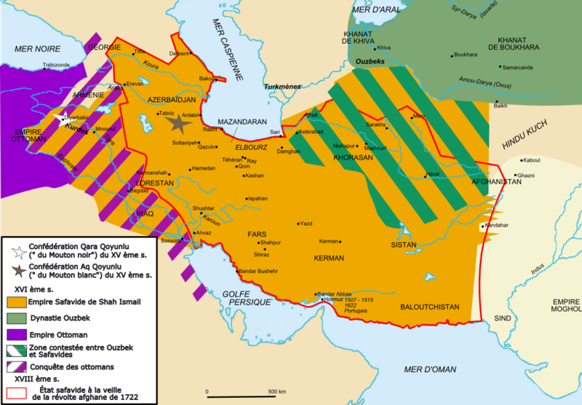
\includegraphics[width=0.9\textwidth]{CourantsIslamContemporain/ImagesCourantsIslamContemporain/empireSafavide.png}

    
\end{figure}


\begin{figure}[h!]
    \centering
        \sidecaption{Apogée et perte de l'empire Moghol : Au XVIII, il est réduit au Rajastan.
}
 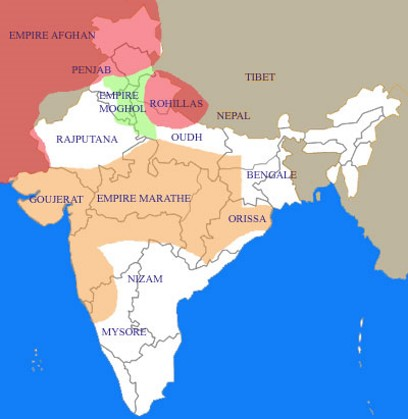
\includegraphics[width=0.44\textwidth]{CourantsIslamContemporain/ImagesCourantsIslamContemporain/Inde18.jpg}
  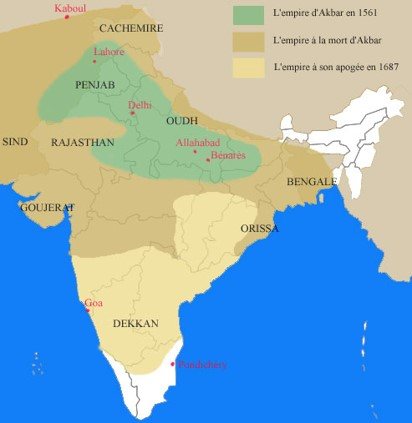
\includegraphics[width=0.44\textwidth]{CourantsIslamContemporain/ImagesCourantsIslamContemporain/empireMoghol.jpg}
\end{figure}

\begin{figure}[h!]
    \centering
        \sidecaption{Déclin Empire Ottoman
}
 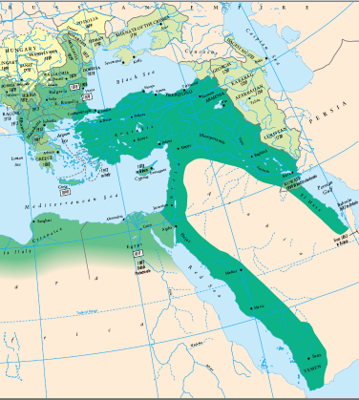
\includegraphics[width=0.5\textwidth]{CourantsIslamContemporain/ImagesCourantsIslamContemporain/declinEmpireOttoman.png}
\end{figure}
 
 \paragraph{Raisons économiques} Les portugais contournent l'Afrique et contournent les empires musulmans.  
 \paragraph{crises politiques} au sein de ces empires, trop grands. 
 \paragraph{Des voisins puissants} Ces Etats vont perdre des territoires face à des puissances qui ne sont pas musulmanes. L'empire Safavide est attaqué par les Ousbeks. L'Empire Moghol en XVIII siècle s'effondre devant l'empire Marathe (Hindou). L'empire Ottoman resiste mais décline depuis 1686 (siège de Vienne). 
 \begin{itemize}
     \item  {Affaiblissement des sultanats Indonésiens} face aux Hollandais. Java est annexé en 1800. 
  \item {En Chine} les musulmans Chinois (Hui) subissent des pressions des Manchous.
   \item  {Afrique} Les bambaras conquièrent Djenné, Tombouctou et Gao. Les portugais en Océanie. 
  \item {En Asie Centrale}, avancée des Russes (XIVII : Kazakstan et reste de l'Asie Centrale au XIX).
 \end{itemize}

 \paragraph{A la fin du XVI} 1591 : deuxième millénaire de l'Islam; sentiment millénariste. \mn{Calendrier lunaire, donc décalage}
 
 
 
\subsection{Problèmes doctrinaux et religieux}

\paragraph{Un raidissement des écoles juridiques au XVII}
Elles s'accusent les unes les autres de ne pas être juste, sentiment de division du monde sunnite.

\paragraph{Décadence du monde Soufi} On a tendance à considérer les soufis comme à la marge du monde musulman. Pourtant, elles ont joué un rôle social déterminant voire politique. Or, à l'époque, elles sont en crise.
\begin{itemize}
    \item {En faisant des Etats dans l'Etat} 
\item {Laxisme spirituel} Un soufi n'est plus tenu de suivre les prescriptions de l'Islam.
\item {Un rôle de plus en plus important du Sheykh}, le maitre spirituel de la Confrérie, qui transmet la \emph{Baraka}.
\item {Des pratiques spéctaculaire} Le fakirisme. le \emph{Dhikr}, rappel du nom de Dieu et l'on atteint l'Etat de transe, et vont marcher sur des braises. 

\end{itemize}



%------------------------------------------------
\section{L'aspiration au
  renouveau}
\subsection{Millénarisme}


 \begin{Def}[rapport au temps Involutif]
 L'Islam se tourne vers le passé, en Islam, les prophètes viennent toujours rappelés ce qui a été donné à l'origine. et le problème est que les hommes déforment le message transmis. Donc Dieu envoie de nouveaux prophètes pour restaurer le message originel. \textit{le temps corrompt.}
 
 \end{Def}
 vs Evolutif. 
 
 Ce qui fait que Mohammad est le dernier des prophètes, c'est que le message est transmis intact, pour la première fois, donc plus besoin de nouveaux prophètes. Autant, la \textit{pratique} peut se corrompre. 
 Un hadith dit : 
 \begin{quote}
     Slt un dixième de la pratique suffira pour sauver le monde.
 \end{quote}
 
 \begin{Def}[Moujaddid]
 de la racine JDD, nouveau, celui qui renouvelle l'Islam pour le mettre tel qu'il était à l'origine. 
 \end{Def}

 
 \begin{Def}[tajdid]
 Tajdid, le renouveau, qui doit venir régulièrement. Chaque siècle Dieu envoie un \textit{Moujaddid} selon un Hadith du Prophète.
 \end{Def}
 
 
 Il peut y en avoir plus mais à chaque siècle, il y a un grand moujaddid, savant, qui ne fait pas forcément au sein de la communauté. 
  \begin{Ex}
 Ghazali est considéré comme un Moujaddid
 \end{Ex}
 \sn{On retrouve cette tension dans toute religion entre respect de la forme et de fidélité au message d'origine}
 
 \subsection{Quelques grandes figures de la \textit{pre-Reforme}}
 

\paragraph{Ahamad Sirhindi} (Inde, 1564-1624) , essaye de rénover l'Islam et réforme une confrérie, la \emph{Naqshbandiyya} réformée (mujaddidi). 
\paragraph{Muhaddidi} Restaurer le monde musulman et restaurer l'Islam dans sa pureté originelle. Il va opposer 
\begin{itemize}
    \item le \emph{taqlid}, l'imitation (péjorative, servile, non réfléchie) et
    \item l'\emph{ijtihad}, l'effort d'interprétation du Coran et de la Sunna. Retourner aux sources scripturaires pour restrouver le sens authentique de l'Islam
    \item pour éliminer la \emph{bid'a}, très péjoratif, l'innovation
\end{itemize}  

On peut distinguer deux courants : un courant plus libéral et l'un plus fondamentaliste :
\begin{itemize}
    \item le rapport à la Tradition : fondamentaliste ne vont considérer que le Coran et la Sunna, en critiquant les élaborations savantes de l'Islam. 
    \item ce sur quoi va porter l'\emph{ijtihad}, soit limité sur les versets peu clairs du Coran, soit plus large pour le savant et les différentes sciences qui vont être convoquées pour l'ijtihad.
\end{itemize}


\paragraph{Muhammad 'Abd Al-Wahhab } 'Arabie, 1703-1792). Voir p. \pageref{Theol:AlWahhab}

\paragraph{Shah Wali Allah} (Inde, 1703-1762), \label{Theo:waliAllah} a eu les mêmes professeurs que Al-Wahhab ! et l'un des premiers à traduire le Coran dans une langue vernaculaire (en persan). Effort d'acculturation dans le contexte Moghol et Indou. 




 
%------------------------------------------------
\section{Les voies du renouveau} 
\subsection{Les confréries soufies}

La création de néo-confrérie
\begin{itemize}
    \item lutter contre un laxisme moral
    \item lutter contre le pouvoir du Sheykh.
    \item insister sur le côté social, en prenant en charge la société (vs gnosticime ?).
\end{itemize}
\mn{Soufi : \pageref{Def:SoufiNaqchabandiya}, \pageref{Def:Soufiqādirīya} }




\paragraph{Ahmad Al Tijani} (Algérie 1737, 1815). Et fonde la \emph{\textbf{tijaniyya}}, un groupe toujours très présent en Afrique du Nord. Normalement un Sheykh insiste sur la chaine d'initiation qui remonte au prophète. Lui, va être initié directement en rêve par le Prophète.

\paragraph{Abdurrauf al-Singkili} (Aceh, Indonésie, 1615-1693)

\paragraph{Abdelkarim al-Samman} (Soudan, 1718-1776) => sammaniyya

Au sénégal, aussi une confrérie de type réformée. 
\mn{A completer carte Carte moderne. Il y avait 24 confréries soufis en Arabie avant le Wahhabisme}




%---------------------------------------
\subsection{Les centres de pèlerinage : La Mecque et Médine}

La Mecque et Médine jouent un rôle essentiel, du fait du Hajj. Du fait de l'Empire Ottoman, il y a pacification des parcours du pélerinage, par ailleurs incités par l'Empire.
Et par ailleurs, des centres de formation s'implémentent à la Mecque.  On en profite pour étudier. Se croisent des savants de différentes origines.
Non seulement les centres d'étude mais aussi les confréries, avec leur Sheykh les plus importants s'installant à Médine ou la Mecque. Ils sont initiés à l'enseignement Moujaddidi et vont réformer la confrérie à laquelle ils appartiennent, selon un modèle qui se répète.




%------------------------------------------------
\section{Un aspect particulier : les jihads aux marges du monde   musulman} 


\begin{figure}[h!]
    \centering
        \sidecaption{Le « renouveau » des marges du monde musulman (XVIIIe-XIXe
siècle)  \emph{L'atlas de l'islam depuis 1500}, F. Robinson, Nathan, 1987  
Des petits Etats vont se créer sur des bases confrériques et dont la mission de faire le jihad.
}
 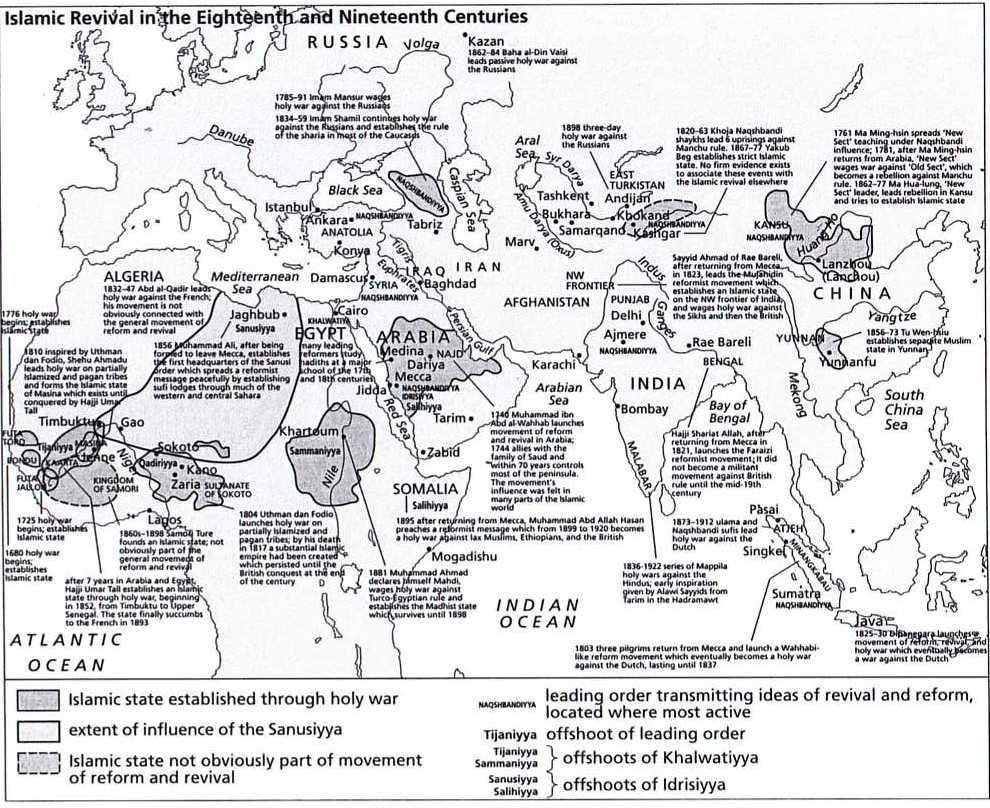
\includegraphics[width=\textwidth]{CourantsIslamContemporain/ImagesCourantsIslamContemporain/image1.jpeg}

    \label{fig:le-renouveau-des-marges-du-monde-musulman-xviiie-xixe-siuxe8cle}
\end{figure}


\subsection{Situation particulière des zones marginales}


Pourquoi on les retrouve aux marges du monde musulman ? Il y a un besoin de purification et l'islamisation par rapport à des populations hétérogènes. Mais aussi, parce que ces zones ne sont pas controlées par les grands empires musulmans qui ne tolèrent pas ces confréries.
Le jihad se porte d'abord sur les musulmans eux-mêmes, pour qu'ils deviennent musulmans puis contre les puissances extérieures ou non musulmanes qui controlent ces zones. 

\paragraph{Une structure Etatique} Le Sheykh est le chef, \emph{Commandeur des Croyants} - on fait référence aux premiers temps musulmans, on prête allégeance, et avec une approche puritaine, très forte pratique. \mn{Des analogiques avec DAESH, qui se réfèrent eux aussi aux temps de l'Islam}

\paragraph{Une accélération de l'Islamisation}


\subsection{Quelques exemples}

\paragraph{Spectre Temporel 1680-1920}{1680, Etat de Bondou} Afrique de l'Ouest jusqu'e l'Etat Mahdiste (Somalie) 1899-1920.

\paragraph{Chine - Ma Ming-hsin} Réveil religieux des communautés chinoises sous la pression des Manchous. Ma Ming-hsin (1719-1781) lorsqu'il est à la Mecque, il fonde une confrérie réformée, la \textit{Nouvelle Secte} et entre en opposition contre les autorités locales, qui appelle en soutien la dynastie Manchoue des Ming. Ming-Hsin est décapité. Il y aura d'autres révoltes plus tard, du Kan-Su et du Chen-Si (1862) et du Yunnan (1856)

\paragraph{Indonésie - Jajji Miskin} Le mouvement Padri à Sumatra (1803-1845). Après le Hajj, en 1803, il prend le contrôle de villages et va imposer sa vision de l'Islam, interdit les pratiques populaires et proclament le Jihad contre les autres villages et les pouvoirs. 1820 : les Hollandais reviennent dans la région et on a une transformation de ce mouvement contre un Jihad contre les Hollandais. Eliminé par les Hollandais.

\paragraph{Nigéria - Califat de Sokoto} Uthman da Fodio (1755-1817) issu d'une famille de savants musulmans, l'enseignement lui vient par la fraderyya\sn{revoir} et crée une communauté qui le reconnait comme \textit{commandeur des Croyants}, s'oppose aux pouvoirs locaux et va être défait par la Grande Bretagne.


\begin{Synthesis}
\begin{itemize}
Ce renouveau : 
    \item Avant la rencontre de l'Occident
    \item lié à des thèmes de crises internes
    \item des thématiques que l'on retrouvera : retourne aux sources scripturaires
    \item C'est assez fascinant de voir la circulation des idées, liée autour du \textit{Hajj}
\end{itemize}


\end{Synthesis}

%------------------------------------------------

 



 



\paragraph{Soufis du Badakhshân : un renouveau confrérique entre
l'Inde et l'Asie centrale}
\mn{Alexandre Papas, \emph{Cahiers d'Asie Centrale}, n° 11-12, 2004, p.
87-102 (extraits -- texte expurgé)}
 
 
\subparagraph{Éléments de biographie d'un soufi
badakhshânais} 
\mn{le Badakhshân est entre l'Afghanistan et le Tajikistan}
\begin{quote}
Mawlânâ Mîr Ghiyâs al-Dîn \label{Theo:MawlanaMirGhiyasAlDin} naît en 1117/1705-06 dans la petite localité
de Hisârak, située au cœur du district de la ville de Jirm. Le
grand-père de Mawlânâ a émigré du village de Dahbîd, non loin de
Samarcande, en direction du Badakhshân. La \emph{silsila}\sn{Génération} de la famille
remonte au Prophète et, sur dix générations, au frère d'un grand saint
Kubrawî et découvre une généalogie \textit{soufie}. C'est donc au sein d'une des
grandes familles \emph{muhâjir}\sn{Emigré, en référence aux premiers musulmans qui ont suivi le Prophète à Médine} de l'aristocratie religieuse du
Badakhshân que naît Ghiyâsî.
\begin{figure}[h!]
    \centering
        \sidecaption{Asie Centrale. On oublie parfois le rôle important de ces états tampon comme lieux d'échange
}
 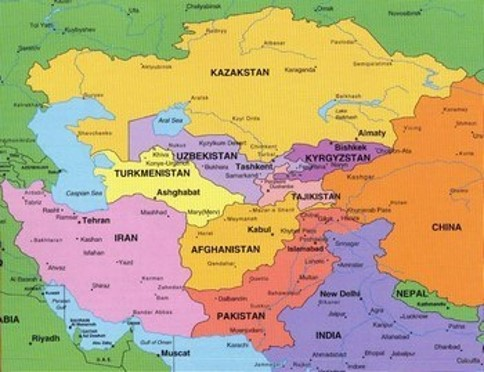
\includegraphics[width=\textwidth]{CourantsIslamContemporain/ImagesCourantsIslamContemporain/AsieCentrale.jpg}
 
\end{figure}

{[}\ldots{]}

C'est précisément pour l'Inde -- destination qui concurrence la
Transoxiane savante, en particulier Boukhara, surtout depuis le XVIe
siècle -- que part le jeune Ghiyâsî âgé de 14 ans en quête d'initiation \sn{soufi}.
Cet exil de l'adolescent fait l'objet de deux contes hagiographiques :
 

\begin{itemize}
\item
 
  Le futur shaykh de Ghiyâsî, Shâh Walî Allâh, qui a quitté Sirhind pour
  entreprendre un pèlerinage au mausolée de Bahâ' al-Dîn Naqshband\sn{le fondateur de la confrérie réformée Naqshandayyi} non
  loin de Boukhara, stationne au Badakhshân, à Jirm, chez le père même
  de Ghiyâsî. Le shaykh demande alors à ce dernier de lui amener ses
  enfants, mais perçoit par claire-vue qu'on lui dissimule le jeune
  Mawlânâ qui, en état de \emph{majzûb}\sn{Ils peuvent faire des choses indécentes} « ravi en Dieu », suscite la honte de
  sa famille. À sa vue le shaykh indien cite un vers de Ni'mat Allâh
  Walî Kirmânî. Et au jeune Ghiyâsî de prononcer miraculeusement le
  second vers du distique. Walî Allâh annonce alors qu'à son retour de
  Boukhara il prendra le jeune homme comme disciple et l'emmènera en
  Inde.
  
\item
 
  Dès l'âge de 9 ans Mawlânâ refuse les conseils de sa famille et se
  distingue des autres enfants. Plusieurs nuits, au cours de rêves, lui
  apparaît un homme illuminé qui lui enjoint de partir pour l'Inde où
  lui est promise la rencontre d'un grand saint soufi. Malgré le refus
  de ses parents qui souhaitent marier leur fils, Ghiyâsî parvient à
  quitter le Badakhshân quelques années plus tard. Parvenu à Lahore et
  après un nouveau rêve révélateur, il attend de nombreux jours au
  couvent de Khwâja Khwândamîr, un khalîfa de la Naqshbandiyya, jusqu'au
  jour où il rencontre Shâh Walî Allâh.
 
\end{itemize}

 
Restent les faits : après une formation classique en \emph{madrasa} à
Delhi où le novice rencontre ses premiers maîtres, il devient à Lahore
durant douze années le disciple d'un fameux maître Naqshbandî Mujaddidî.
Il interrompt une unique fois son initiation lorsque le shaykh lui
confie la mission de se rendre au Cachemire afin d'aller chercher un
homme qu'on prétend thaumaturge et que Walî Allâh souhaite convertir à
l'islam et initier à sa \emph{tarîqat}\sn{confrérie}. Au terme de ses douze années de
noviciat, le shaykh lui enjoint de retourner à sa terre natale pour
propager la confrérie. De retour au Badakhshân, Ghiyâsî âgé de trente
ans environ et qui a obtenu le rang de \emph{mawlawiyyat}\sn{maître}, fait office
d'enseignant à la \emph{madrasa} Jâmi'-i Islâmî du district de Jirm. Il
est ensuite convié à Fayz Âbâd à la cour de Sultân Shâh, laquelle abrite
des savants et des poètes venus d'Inde et d'Iran, dont certains
acquièrent grande réputation. C'est là que Ghiyâsî compose son œuvre
poétique et mystique. C'est également là, de son \emph{khânaqâh}\sn{couvent soufi, Ḵānqāh ou ḵānāqāh, fut d'abord un lieu destiné à abriter les spécialistes et savants religieux musulmans (‘ulamâ’), une sorte d'équivalent des couvents chrétiens. Ces établissements ont été ensuite réservés aux soufis.}, qu'il
dirige son enseignement, suivis par de nombreux disciples venus de
toutes les régions alentours. Le soufi badakhshânais devient aussi le
directeur spirituel de Sultân Shâh. Et lorsque ce dernier est capturé à
Qunduz par les ouzbeks du Qataghân en 1179/1765, le vieux maître
conseille durant trois ans le fils et suppléant du shah emprisonné, Mîr
Muhammad Shâh. D'un tel succès et d'une telle influence, Ghiyâsî
apparaît comme l'un des principaux promoteurs de la Mujaddidiyya dans le
Nord de l'Afghanistan.

{[}\ldots{]}
\end{quote}

\begin{Prop}
On retrouve des noms : Walî Allâh (cf p. \pageref{Theo:waliAllah}; l'importance du réseau confrérique; et rôle social (il devient le conseil du sultan).
\end{Prop}

\subparagraph{Savants et soufis au croisement du
Badakhshân}
Le Pamir est un sanctuaire pour les savants hétérodoxes ou bannis (cf Unwân banni d'Egypte du fait de sa lutte sociale).

\begin{quote}
Malgré les obstacles géographiques et en dépit des troubles politiques
qui affectent la fin du XVIII\textsuperscript{e} siècle, le Badakhshân
reçoit la visite de savants religieux qui, pour certains, décident de
s'y installer et interrompent définitivement leur voyage vers l'Inde ou
vers la Transoxiane. Il faut rappeler ici que le Pamir a, de façon
continue dans l'histoire, servi de sanctuaire à des individus frappés
d'ostracisme ou fuyant la répression dans leur région natale. Mais au cours du
XVIII\textsuperscript{e} siècle le sanctuaire se mue en lieu de
renaissance où fleurissent \emph{madrasa}\sn{lieu d'enseignement religieux} et couvent soufis. Le
\emph{Armaghân-i Badakhshân} mentionne le cas de deux étudiants de
Peshawar, Mîr Ahmad Mujaddidî dit `Izhâr' (m. 1259/1843) et son frère
Muhammad Anwar qui, à une date indéterminée durant le règne de Mîr
Muhammad Shâh, se rendent d'abord à Boukhara afin d'obtenir les
compétences du rang de \emph{`âlim}\sn{savant} et qui, lors de leur retour,
s'installent et officient au Badakhshân, pour le premier à Jirm, pour le
second à Bahârak.

Un autre cas de figure est celui, analogue à Ghiyâsî, de ces
badakhshânais qui partent se former aux sciences religieuses, et
éventuellement au soufisme, dans les grands centres de savoir du monde
musulman, proches ou lointains. De ce point de vue, le cas le plus
intéressant -- et malheureusement le plus douloureux faute
d'informations suffisantes et dans l'absence de vestiges de son œuvre --
est celui de Sayyid Abâ al-Hasan « `Unwân ». Né à Jirm en 1123/1711, il
quitte le Badakhshân pour Boukhara afin d'acquérir une formation
théologique. De là `Unwân se rend au pèlerinage de La Mecque et à
Médine, puis il s'installe durant 18 ans en Egypte, probablement au
Caire, où il poursuit son acquisition des sciences islamiques classiques
et commence à enseigner. Mais `Unwân ne se contente pas de dispenser un
enseignement religieux, il prend parti pour les classes populaires
égyptiennes et contre leur oppression par les propriétaires terriens.
C'est du moins la réputation qu'il gagne selon le \emph{Armaghân-i
Badakhshân}, et qui lui vaut d'être banni d'Egypte. `Unwân part alors
pour Istanbul, rejoint Boukhara et reprend son enseignement. `Unwân, qui
prône l'unité de la Communauté des Croyants (\emph{umma}), décide
d'aller prêcher la concorde (\emph{âshtî}) dans le Caucase, peut-être au
moment de l'activisme Naqshbandî de Shaykh Mansûr dans les années 1780.
Mais il renonce à son projet et entre dans une retraite spirituelle
jusqu'à sa mort en 1206/1791, sans être retourné au Badakhshân.
{[}\ldots{]}

\end{quote}

\begin{Prop}
 Dans le deuxième paragraphe, `Unwân se forme à la Mecque et Médine (rôle du pélerinage), rôle social en Egypte et pas seulement religieux. L'importance aussi de l'Unité, l'\textit{Umma}. 
\end{Prop}
 
\subsection{Liste des neo confréries}

\paragraph{Naqshbandiyya}: La Mecque, Damas, Yémen, Inde, Asie Centrale \label{Def:Naqshbandiyya}
                     => Caucase, Chine Occidentale + Orientale, Sumatra.

\paragraph{Qadiriyya}: Proche Orient, Irak, Inde, Asie centrale 
                    => Indonésie (Java, Aceh), Caucase, Afrique

\paragraph{Khalwatiyya}: Egypte => nombreuses branches en Afrique :

\begin{itemize}
    \item \textit{Tijaniya}: Algérie => Afrique de l’Ouest
    \item \textit{Sammaniyya}: Soudan
    \item \textit{Idrisiyya}: Maroc => Sanusiyya (Lybie), Sahiliyya (Somalie),
    \item \textit{Murghaniyya} (Erythrée)
\end{itemize}- 
 
%-----------------------------------------------
\subsection{bibliographie}

\begin{quote}


AZRA, Azyumardi \emph{The Origins of Islamic Reformism in Southeast
Asia}, Asian Studies Association of Australia/KITLV Press, Leiden, 2004.

PAPAS, Alexandre \emph{Soufisme et politique entre Chine, Tibet et
Turkestan}, J. Maisonneuve, Paris, 2005.

*ROBINSON, Francis \emph{Atlas de l'Islam depuis 1500}, Nathan, Paris,
1987 (dispo à la FELS)

*VOLL, John R. « Foundation for renewal and reform », in John L.
Esposito ed., \emph{Oxford History of Islam}, Oxford University Press,
1999, pp. 509-547.
\end{quote}
\chapter{Un fruit du « pré-réformisme » : le wahhabisme}
\mn{ \emph{(31/01/2022)}}

%---------------------------------------------------------
\section{Le wahhabisme}
\paragraph{Pourquoi en parler} C'est un courant qui a presque trois siècles, avec une évolution dans le monde du musulman qui a évolué. Il faut penser l'Islam contemporain dans son contexte.

 
  \subsection{Muhammad Ibn al Wahhab
  (1702-1792)} 
  \label{Theol:AlWahhab}
  
\paragraph{Origine} Son père est \emph{qadi}\sn{juge} et enseignant. Dans le Hadz. Fait un pélerinage à la Mecque. Renouveau

\paragraph{Formation et premières prédications} Proclame le \emph{Tawhid} l'unicité et lutte contre toutes les pratiques "déviantes". Il se heurte aux autorités locales et retourne donc à la Mecque. Il se forme là avec des maîtres d'Arabie et Indien. Puis se rend à Basra, à un autre maître. C'est là qu'il rencontre les si'ites. Il se heurte de nouveau aux autorités locales. Il rentre en Arabie mais \textit{son père y est hostile}. Ce n'est pas un grand savant mais un lettré. 
 
\paragraph{L'alliance avec Ibn Se`ud} Alliance matrimoniale avec un chef de tribu de la Mecque. Il se rend indésirable et il est obligé de partir et il arrive dans le village de Dariya et il y rencontre un autre chef de village, Mohammed Ibn Se'ud, alliance elle aussi politicolo-religieuse et matrimoniale en 1744. Ibn Se'ud accepte la doctrine et al Wahhab légitime l'acquisition de terre par Ibn Se'ud. 

Wahhab enseigne beaucoup  : il écrit beaucoup à des savants (\emph{Oulema}) à l'intérieur et l'extérieur du royaume de Ibn Se'ud. \textit{selon un modèle prophétique}, Mohammad ayant écrit au Basileos,... 

\paragraph{Un développement politique} Conquiert toute l'Arabie Saoudite. En 1818, c'est la fin du premier état wahhabite car l'empire ottoman intervient et execute le fils de Ibn Se'ud.
    
 Il s'appuie sur deux auteurs : 
\begin{itemize}
    \item Ibn Taymiyya (1263-1328), \label{Theol:Taymiyya2} \sn{cf p. \pageref{ibn-taymiyya}}, un vrai penseur
    \item Ibn Qayyim (1292-1350) un de ces disciples
\end{itemize}
 
Ibn Wahhab insiste sur le retour à la source mais en fait il lit le Coran à travers ces deux auteurs.

\paragraph{Une doctrine condamnée} Son père et son frère s'opposent à lui. Une fatwa contre lui du fait de sa critique sur les différentes écoles juridiques et le fait qu'il exclut de la communauté musulmanes ceux qui ne pensent pas comme lui. 

  \subsection{La doctrine wahhabite} 



  \paragraph{Nécessité du retour aux sources} Accentuation des sources, bien sûr le Coran. 
  \begin{itemize}
      \item  \item  Wahhab s'éloigne d'une lecture du Coran ligne à ligne mais propose une analyse \textit{thématique}.
  \item Il rejette aussi le besoin d'une \textit{médiation} humaine pour comprendre le Coran. Il s'oppose aux \emph{Ashraf}, les descendants du prophète \sn{Les Ashrafs ont un statut particulier dans l'Islam} ainsi qu'aux \emph{Imams} dans le si'isme, ainsi que les \emph{sheykhs} soufis.
  \begin{Prop}
  Il n'y a pas besoin de sciences particulières pour accéder au sens du Coran, d'après Wahhab. 
  \end{Prop}
  \item il suis les \emph{Hadiths}, la seule exégèse possible, la \textit{sunna} et rejette les grands commentaires classiques du Coran.  Cela va jusqu'à critiquer la tradition des 4 premiers Califes \textit{bien guidés}. Abu Bakr avait détourné la \textit{zakat} pour ses propres dépenses.
  \item Il reprend la distinction d'Ijtihad, qu'il limite aux versets aux versets obscures, contre le taqlid. Il s'oppose à deux principes de l'Ijtihad : qiyas (recours par analogie : alcool et drogue), \textit{ijama} (consensus des savants : on considère que cela fait autorité \sn{Infaillabilité de la communauté dans les Hadiths}), et le \textit{ra'y}, l'opinion personnelle du juriste. 
  
  \end{itemize}
 
 \begin{Prop}
 Il conteste les principes sous-jacents aux savants qui l'ont précédés. Il y a une tension entre son ambition de revenir au Coran mais en parallèle en se mettant en filiation avec Ibn Taymiyya
 \end{Prop}
 
 
  \paragraph{Une notion centrale : le \emph{tawhid} (unicité divine)}
  
  \mn{{Extraits du \emph{Kitab at-tawid} (Livre de
l'unicité divine) de Muhammad Ibn Wahhab} . {Chapitre 1} : \emph{Tawhid}
Traduction et édition établies en Arabie Saoudite. Allah est traduit par Allah et non Dieu, alors qu'en Arabe, Dieu est traduit par Allah y compris pour les chrétiens arabes. }

\begin{quote}
\emph{Allah-ta`ala} a dit : « Je n'ai créé les djinns et les hommes que
pour qu'ils M'adorent (1 :56)\ldots Et très certainement nous avons
suscité dans chaque communauté un message pour leur dire d'adorer Dieu
et d'écarter le Rebelle (16 :36)\ldots Et voilà que ton Seigneur a
décrété que tu dois n'adorer que Lui et faire preuve de bonté envers tes
parents (17 :23)\ldots Adorez Dieu et ne lui donnez quelque associé que
ce soit (4 :36)\ldots Venez, je vais vous réciter ce que votre Seigneur
vous a interdit ; - ceci : Ne lui associez quoi que ce soit\ldots(6
:151-153) ». Ibn Mas`ud a dit : « Quiconque se propose de vérifier le
testament du Prophète Muhammad (SWA) -- un testament sur lequel le
Prophète a apposé son sceau, qu'il lise ces mots d'Allah : « Venez, je
vais vous réciter ce que votre Seigneur vous a interdit ; - ceci : Ne
lui associez quoi que ce soit\ldots Voilà ce qu'il enjoint » (6 :
151-153)


Mu`adh Ibn Jabal raconta : « Je montai derrière le Prophète (SAW) quand
il me dit : « Ô Mu`adh ! Sais-tu ce que les créatures d'Allah Lui
doivent et ce qui leur est dû ? » Je répondis : « Allah et son Prophète
savent mieux ». Il continua : « Ce que les créatures d'Allah Lui
doivent, c'est de ne jamais associer qui que ce soit avec Lui. Ce qui
leur est dû, c'est qu'il ne punira aucune personne qui ne Lui associe
pas un autre ». Je dis :

« Ô Prophète d'Allah, est-ce que je peux annoncer la bonne nouvelle aux
gens ? » Il répliqua : «Non ! Ne leur dis rien de peur qu'ils comptent
sur la promesse et manquent à leurs devoirs envers Lui». Ce hadith est
mentionné dans deux \emph{Sahihs}.


D'autres points :


\begin{enumerate}

\item
  \begin{quote}
  La sagesse dans la création du djinn et de l'humanité.
  \end{quote}
\item
  \begin{quote}
  Le service à Allah consiste en le \emph{tawhid}. Car, à l'opposé du
  \emph{tawhid} se trouve l'aliénation d'Allah. (\ldots)
  \end{quote}
\item
  \begin{quote}
  La sagesse d'envoyer des prophètes. (\ldots)
  \end{quote}
\end{enumerate}
  \end{quote}
  
On trouve une accumulation de versets coraniques sur le thème, puis des hadiths du prophète. Le grand péché par excellence, c'est le \emph{shirk}, l'associationisme des Dieux à Dieu. Or Wahhab va plus loin. 

\begin{quote}


\emph{Allah-ta`ala} dit : « Ceux qui ont cru et n'ont point revêtu de
prévarication leur foi\ldots{} » (6 : 82).

(\ldots) Abu Sa`id al Khudriyy rapporta que le Prophète d'Allah (SWA) a
dit : « Quand Musa {[}Moïse{]} demanda à Allah de lui enseigner une
prière qu'il puisse réciter à chaque fois qu'il pensait à Lui ou qu'il
L'évoquait, Allah répondit : « Dis, ô Musa, qu'il n'y a d'autre Dieu
qu'Allah. Musa dit : « Ô Seigneur, tous tes serviteurs prononcent ces
mots ». Allah dit : « Ô Musa, si les sept cieux et tout ce qu'ils
renferment, et les sept terres aussi, si tout cela était pesé contre
cette phrase : « Il n'y a d'autre Dieu qu'Allah », cette dernière
pèserait plus lourd ». Ibn Hibban rapporta cela également et al-Hakim
compléta sa version. Al-Tirmidhi enregistra, avec peu de rédaction, le
récit de Anas à l'effet qu'il entendit le Prophète d'Allah (SWA) dire :
« Allah dit : « Ô Homme ! Si tu venais à Moi avec tous les sacs du monde
remplis de tes péchés, mais avec le témoignage que tu n'associes rien à
Moi, Je viendrais à toi avec tous mes sacs remplis de miséricorde et de
pardon ! ».

    
\end{quote}

\begin{Synthesis}
Si on respecte le \emph{Tawhid}, cela suffit à pardonner les péchés, mais important de respecter les principes de l'Islam (c'est pour cela que c'est caché)
\end{Synthesis}

\paragraph{Distinction au sein du Tawhid } 
\begin{Def}[Le grand Shirk ]
Il distingue le \emph{tawhid rububiyya} (l'unicité de souverainté du monde) avec le \emph{tawhid uluhiyya} (de divinité) : ne reconnaitre aucun intermédiaire entre Dieu et les hommes. Il ne peut y avoir de dévotion que pour Dieu seul : les saints, les soufis, les Imams.
\end{Def} 
Al Wahhab introduit une critique fondamentale contre le soufisme. 

\paragraph{Le petit Shirk} 
\mn{{Chapitre 4} : La crainte du \emph{shirk}}
\begin{quote}
Allah -- qu'Il soit loué et glorifié -- dit : « Non, Dieu ne pardonne
pas qu'on Lui donne quelque associé. En deçà, Il pardonne à qui il veut
» (4 : 48, 116)

(\ldots) Dans le hadith, nous lisons : « Ce que je crains le plus pour
vous, c'est le moindre \emph{shirk}. Quand on lui demanda ce que
c'était, le Prophète répondit : « l'hypocrisie ». Dans le Sahih
d'al-Bukhari, nous lisons que Ibn Mas`ud reporta : « Le Prophète d'Allah
(SWA) a dit : « Celui qui rencontre Allah le jour du Jugement sans Lui
avoir associé qui que ce soit ira au Paradis, et celui qui le rencontre
ayant fait le contraire sera consigné en Enfer ».
\end{quote}
\begin{Def}[le Petit Shirk]
Toute attitude de l'homme qui ne sert pas Dieu. il relève aussi de l'attitude morale.
\end{Def}

\begin{Ex}[L'appel à témoigner qu'il n'y a d'autre
Dieu qu'Allah]

\mn{{Chapitre 5} : }
\begin{quote}
\emph{Allah-ta`ala} a dit : « Dis (ô Muhammad) : `\,`Voici mon sentier,
j'appelle à Dieu'\,' » (12 :108)

Ibn `Abbas (RA) rapporta : « Quand le Prophète d'Allah (SAW) envoya
Mu'adh à al-Yaman, il lui recommanda : `\,`Quand tu rencontres des gens
du Livre, que ta première action soit de leur demander de témoigner
qu'il n'y a d'autre Dieu qu'Allah'\,' ». Selon un autre récit, «
\ldots{} de leur demander de réaliser l'unicité d'Allah. S'ils
t'obéissent, informe-les qu'Allah leur a imposé la \emph{salat} cinq
fois par jour. S'ils t'obéissent en cela, alors informe-les qu'Allah
leur a imposé le devoir de charité qui doit être perçue des riches pour
être distribué aux pauvres. S'ils t'obéissent en cela, ne touche pas à
leurs autres biens et occupe-toi de la plainte de l'opprimé, car il n'y a aucun obstacle dans son accès à Allah ».
(Rapporté dans les \emph{Sahihs} d'al-Bukhari et de Muslim). (\ldots)
\end{quote}
\end{Ex}



\paragraph{Les Intercessions} L'intercession est limitée à Mohammed, et uniquement aux musulmans suivants Wahhab. On ne peut pas prier le Prophète. Peut être intervient-t-il au jugement dernier.


\mn{{Chapitre 17} : L'intercession}
\begin{quote}
Allah -- qu'il soit loué et glorifié -- a dit : « Et par ceci (le
Qur'an), avertis ceux qui, n'ayant pour eux hors de Dieu, ni ami ni
intercesseur, craignent d'être rassemblés vers le Seigneur\ldots{} » (6
: 51). Dis : « A Dieu l'intercession tout entière\ldots{} » (39 : 44).
Qui peut intercéder auprès de Lui que par sa permission ?... (2 : 255).
Et combien d'anges dans les cieux ? Leur intercession ne met au large en
rien, sauf après que Dieu l'a permis, en faveur de qui il veut et qu'il
agrée » (53 : 26). (\ldots)

(\ldots) En tant que catégorie générale du Jour du Jugement en laquelle
les mécréants croient, l'intercession est rejetée par le Qur'an. Le
Prophète (SAW) nous informa qu'en ce jour « il sera amené devant Allah.
Il se prosternera lui-même et louera Allah, plutôt que de demander à
intercéder. Alors on lui dira : « Lève-toi ! Parle maintenant et tu
seras entendu ! Demande et il te sera donné ! Intercède et il te sera
accordé ! » (\ldots) L'intercession est donc là pour les croyants
sincères et candides. Elle n'est accordée que par la permission d'Allah
et n'appartient pas aux associationistes. (\ldots)
\end{quote}


\paragraph{Tombe du juste}
Condamnation de celui qui invoque Dieu
auprès de la tombe du juste et, a fortiori, de celui qui invoque ce
dernier.
\begin{Ex}[Un exemple de Grand Shirk]
\mn{{Chapitre 20} : Condamnation de celui qui invoque Dieu
auprès de la tombe du juste et, a fortiori, de celui qui invoque ce
dernier.}
\begin{quote}
Dans le \emph{Sahih}, A'ishah (RAA) rapporta : « Umm Salmah raconta au
Prophète d'Allah (SAW) qu'elle avait vue une église remplie d'images et
de statues en Abyssinie. Le Prophète dit : « Ceux-là sont les pires de
tous les hommes : lorsqu'un membre juste et vertueux de leur groupe
meurt, ils bâtissent une église sur sa tombe et y installent toutes
sortes d'images pour lui. Ils sont coupables de deux méfaits : celui
d'invoquer quelqu'un auprès d'une tombe et celui d'installer des images
». (\ldots)

Ainsi le Prophète interdit cette pratique et condamna celui qui la
suivait. Faire le \emph{salat} sur une tombe est également interdit,
même si aucune mosquée n'a été construite sur l'emplacement. Telle est
la signification de la déclaration suivante : « On craignait qu'elle ne
soit prise pour une mosquée ». Les Compagnons n'étaient pas supposés
construire une mosquée autour de la tombe du Prophète. Tout endroit
destiné au \emph{salat} ou tout endroit où le \emph{salat} est accompli,
est une mosquée. Tel l'a déclaré le Prophète (SAW) : « Toute la terre
est pour moi une mosquée, un endroit pur (pour accomplir le
\emph{salat}) ».
\end{quote}

\end{Ex}


  \paragraph{La question du \emph{jihad}} La question de la violence chez Wahhab. Il faut repartir de la position kharijite. Un calife doit respecter la religion de façon exemplaire. s'il ne le fait pas, il est \emph{Takfir}, mécréant. Or la vision sunnite a jugé que c'est Dieu uniquement qui jugera si un musulman est un non-musulman. Ibn Taymmayyia s'élève contre les souverains Mongols : : les souverains mongols sont certes musulmans puisqu'ils ont adopté la foi musulmane mais en surface.  Wahhab va reprendre ce concept et ceux qui n'adhèrent par au \emph{shirk} sont apostats. Un germe de violence.
  
  \begin{Synthesis}
  On voit donc l'extension du concept de Ibn Taymmayyia sur le Takfir à tout le shirk, et donc en pratique en non respect du wahhabisme.
  \end{Synthesis}
 
 Mais il n'y a pas de volonté de jihad dans le wahhabisme. On peut même faire des traités avec des non-musulmans.
 
  \section{Le devenir du wahhabisme} 
 
  
 

% ------------------------------ 
\subsection{Les trois Etats Saoudiens} 

 
  {\paragraph{1744 -1818}: une première expansion}
 
 
\emph{1744} alliance Ibn Se`ud /Ibn al-Wahhab
 
\emph{1786} conquête du Najd (`Abd-al-`Aziz)
 
\emph{1792} mort d'Ibn al-Wahhab
 
\emph{1806} conquête de La Mecque
 
\emph{1818} défaite devant les Ottomans
 

 
  {\paragraph{1821-1883}: petit Etat centré sur Riyad (Najd)}
 
  {\paragraph{1901- 2011} : le Royaume d'Arabie Saoudite} Un descendant de Wahhab qui repasse alliance avec la famille de Se'ud et conquiert l'Arabie. 
 
 
\emph{1924} conquête de La Mecque. Abdelaziz Ibn Se`ud prend le titre de
roi et \textit{protecteur des lieux saints}. On détruit les confrérie, on contrôle le pélerinage, on supprime les autres écoles de droit.

\mn{REVOIR}

\emph{1939} début de la production pétrolière \emph{1962} création de la
Ligue islamique \emph{1990} début de la guerre du Golfe.
 

 
\subsection{L'Arabie Saoudite et l'économie
pétrolière} 
 
\paragraph{ {Début de la
production}} 

\begin{quote}
1935: premier forage

1939: premier baril de pétrole

⇒ Cartel américain: l'ARAMCO
\end{quote}

 
\paragraph{{Nationalisation de la
production}}


1973: l'Etat s'approprie 25 \% des droits de l'ARAMCO (1974 : 60\%, 1980 : 100\%)


⇒ Saoudi ARAMCO: 95 \% de la production du pays.

 
\paragraph{Evolution du cours du
pétrole} 

\begin{quote}
1973: premier choc pétrolier (guerre de Kippour) =\textgreater{} de 4 à
15 \$/B

1981-1983: deuxième choc pétrolier (Révolution iranienne + guerre
Iran-Irak) =\textgreater{} 36 \$/B 2006-2008: troisième choc pétrolier
(guerre en Irak) =\textgreater142 \$/baril
\end{quote}

\paragraph{{Rente}}: 1973-2002 =\textgreater{} 200 000 milliards
de dollars au total
 
    Une étude de cas : le wahhabisme en Afrique de l'Ouest
    
\subsection{Le wahhabisme et l'Etat saoudien}

Le wahhabisme accepte une certaine ouverture en Arabie en contrepartie de financement extérieur. On est dans des \textit{concessions} des oulemas. 

\paragraph{La ligue islamique 1962} on étudie gratuitement à la Mecque et à Médine pour propager le wahhabisme.

 
\subsection{Une étude de cas : le wahhabisme en Afrique de l’Ouest}

\paragraph{Des étudiants revenant de la Mecque dans les années 40} et surtout depuis dans les années 70, avec la ligue islamique. 

\paragraph{Un conflit avec les structures soufis}, maraboutisme, très puissantes. On ne priait pas dans les mêmes lieux de culte. 1978 : On  est  loin de  l'époque  où,  en  1978,  Yao  Koum  expliquait  au  Ministre  de  l'Intérieur  qu' \sn{Le wahhabisme à Abidjan Marie Miran-Guyon \url{https://halshs.archives-ouvertes.fr/halshs-01062687/document}}
\begin{quote}
    "obliger  un musulman  orthodoxe (wahhabite)  à  prier  derrière  un  musulman  traditionnel,  c'est  le  contraindre  à renoncer  purement  et  simplement  à  sa  religion,  c'est  l'anéantir  moralement".
\end{quote}


 % -------------------------
\subsection{ {Glossaire}} 


\paragraph{Personnes} `Abd al --`Aziz Abu Bakr

al-Majmu`i al-Sindi

Ibn Taymiyya Muhammad Ibn Se`ud

\paragraph{Lieux}

al-Azhar al-Dir'iyah

al-Uyaynah (Najd). Basra

Hijaz Huraymila Jeddah Najd

\paragraph{Notions}

ashraf : \emph{descendants du Prophète}

da`wa \emph{: prédication}

fiqh : \emph{droit musulman}

hadith \emph{: fait ou dire du Prophète}

hijra : \emph{« exode »}

ijma\emph{` : consensus des ulamas}

ijtihad : \emph{effort d'interprétation}

kufr \emph{: incroyance /} 

kafir \emph{: infidèle, mécréant}

qiyas \emph{: raisonnement par analogie}

salat : \emph{prière rituelle} 

shirk : \emph{associationnisme} 

taqlid
\emph{: imitation (servile)} 

tawhid : \emph{unicité divine}

zakat :
\emph{aumône légale}

 %-----------------------------------------------------
\subsection{Extraits du \emph{Kitab at-tawid} (Livre de
l'unicité divine) de Muhammad Ibn Wahhab}
\mn{Traduction et édition établies en Arabie Saoudite}

\paragraph{{Chapitre 2} : Les vertus du \emph{tawhid} et les
nombreux péchés qu'il expie}



\paragraph{{Chapitre 27} : Les motivations mondaines sont des
exemples de \emph{shirk}}
\begin{quote}
\emph{Allah ta'ala} a dit : « Qui aspire à la vie d'ici-bas et à ses
parures, nous leur solderons ce qu'ils y auront fait : ils ne subiront
pas de perte ! Voilà ceux qui, dans la vie dernière, n'ont pour partage
que le Feu : leurs réalisations d'ici-bas ont crevé ! Nulles sont leurs
œuvres ! (11 : 15-16).

Abu Hurayrah (RAA) rapporta ce hadith \emph{sahih} suivant : « Le
prophète d'Allah (SAW) a dit : `\,`Malheur à l'esclave du dinar !
Malheur à l'esclave du dirham ! Malheur à l'esclave du khamilah !
(\ldots)
\end{quote}
\paragraph{{Chapitre 38} : Obéir aux ulamas ou aux gouvernants
qui légitiment ce qui est interdit ou interdisent ce qui est légitime,
c'est les associer à Allah.}
\begin{quote}
Ibn `Abbas a dit : « Je vous dis que `\,`le Prophète d'Allah (SAW) a dit
ceci et vous dites que `Abu Bakr et `Umar ont dit quelque chose d'autre
?'\,' Le ciel va bientôt vous cracher des pierres sur la tête !! »

Ahmad ibn Hanbal a dit : « Très étranges, en effet, sont ceux qui,
sachant le véritable \emph{isnad} (d'un commandement du Prophète), se
tiennent quand même à l'opinion de Sufyan. Allah lui-même a dit : « Que
ceux donc qui s'opposent à son commandement prennent garde qu'une
tentation ne les atteigne, ou que ne les atteigne un châtiment
douloureux ». (24 : 63). Savez-vous ce que peut être une telle tentation
? C'est le \emph{shirk}. Car, désobéir au Prophète dans certains de ses
commandements, c'est pratiquement comme si on reniait son message et on
s'attirait le Feu.

\end{quote}


\section{bibliographie}

 

\begin{itemize}
\item
 
  IBN AL-WAHHAB, Muhammad \emph{L'unicité de Dieu}, al Qalam, Paris,
  2001.
 


 \item
MENORET, Pascal \emph{L'Énigme saoudienne. Les Saoudiens et le monde
1744-2003}, La Découverte, Paris, 2003.
\item
MIRAN, Marie ; RIALLAND, Maëlle « Dossier Wahhabisme », \emph{Islam et
sociétés au Sud du Sahara}, n°12, 1998, Paris.
\item
MOULINE, Nabil \emph{Les Clercs de l'islam. Autorité religieuse et
pouvoir politique en Arabie Saoudite
(XVIII\textsuperscript{e}-XXI\textsuperscript{e} siècles)}, Paris, PUF,
2011.
\item
  \emph{Histoire de l'Arabie
saoudite}, Paris, Flammarion, 2013.
\item
REDISSI Hamadi \emph{Une histoire du wahhabisme. Comment l'islam
sectaire est devenu l'islam}, Paris, Seuil, 2016.
 \end{itemize}
 
 
\mn{
\href{http://journals.openedition.org/assr}{Archives de sciences
sociales des religions} p. 229-253

\url{https://doi.org/10.4000/assr.21954}}

\section{Les oulémas du palais}

Parcours des membres du Comité des grands oulémas

\hypertarget{ruxe9sumuxe9s}{%
\subsection{\texorpdfstring{\emph{Résumés}}{Résumés}}\label{ruxe9sumuxe9s}}


Véritable matrice idéologique de l'État saoudien et instrument de
légitimation politique et religieuse, la doctrine wahhabite et ses
dépositaires, les oulémas, sont les soutiens indéfectibles de la famille
Sa‛ūd depuis la seconde moitié du e siècle. Cette alliance se renforce,
à partir de 1971, avec la création d'un certain nombre d'institutions
politico-religieuses dont la plus importante est le Comité des grands
oulémas. Si les larges prérogatives, dont dispose cette dernière dans
les domaines politique, religieux et social, poussent l'autorité
politique à vouloir en chapeauter l'action et contrôler l'accès,
l'establishment wahhabite n'en fait pas moins. En effet, l'élite
religieuse saoudienne a adopté des mécanismes d'autorégulation bien
définis pour maintenir son homogénéité et son unité pour mieux dominer
l'espace socioreligieux du royaume. Nous tentons dans cet article, à
partir d'une étude de terrain, de lever le voile sur ces mécanismes en
étudiant les origines sociales et régionales et le cursus honorum des
quarante-cinq oulémas qui siègent ou ont siégé au Comité. Cela permet
d'en ressortir avec le portrait idéal-type de l'ouléma wahhabite
contemporain et de voir dans quelle mesure son parcours le qualifie pour
l'encadrement de la population et du soutien au régime.

\hypertarget{texte-intuxe9gral}{%
\subsection{\texorpdfstring{\emph{Texte
intégral}}{Texte intégral}}\label{texte-intuxe9gral}}

\begin{quote}
\mn{ Paris -- Institut d'Études Politiques,
\href{mailto:mohammednabil.mouline@sciences-po.org}{\nolinkurl{mohammednabil.mouline@sciences-po.org}}}

En s'appuyant sur la doctrine hanbalo-wahhabite, pour légitimer leur
pouvoir et leur hégémonie en Arabie et étendre leur influence dans le
monde musulman, les Āl Sa‛ūd se sont étroitement liés aux oulémas,
dépositaires et interprètes de cet «instrument intellectuel par
excellence de domination politique» en Arabie Saoudite (Al Rasheed,
2007: 28). En échange de la garantie d'autonomie de l'espace religieux
et d'un contrôle plus ou moins étroit de l'espace social, les oulémas
mettent au service de la monarchie saoudienne toutes les ressources
symboliques dont ils disposent pour légitimer ses positions et
sanctifier son action. La consolidation définitive du royaume saoudien,
en 1932, n'a fait que renforcer cette alliance et l'institutionnaliser.

Le flux des revenus pétroliers et la politique de solidarité islamique
menée par la
monarchie saoudienne (Kepel, 2003: 89-92; al-Suwayyigh, 1992: 83-93) a
permis à l'establishment hanbalo-wahhabite de se moderniser en se dotant
de structures administratives et éducationnelles dont la plus importante
est le Comité des grands oulémas. 
\begin{Def}[comité des grands oulémas]
Mise en place en 1971, cette instance,
où siègent en théorie les plus éminents oulémas du pays, et même du
monde musulman, s'est très rapidement imposée comme la principale
instance législative du pays, à côté du conseil des ministres, la
principale instance légitimatrice de l'action politique du pouvoir et le
bouclier idéologique du régime. 
\end{Def}

L'importance que revêt cette
organisation étatique fédérative pour le pouvoir politique saoudien
pousse ce dernier à vouloir en contrôler l'accès et le fonctionnement
pour éviter toute «insubordination» des grands oulémas. De même, l'élite
religieuse veille, à travers ses réseaux formels et informels, à
maintenir sa cohésion et son homogénéité, pour perpétuer l'hégémonie de
son discours, en imposant aux prétendants aux charges «cléricales»
officielles des conditions plus ou moins rigoureuses. Toutefois, aucun
document ne mentionne les conditions que doit remplir un ouléma pour
accéder au Comité. Le seul moyen de lever le voile sur ces conditions
d'accès tacites est de suivre le parcours et le processus de
socialisation des cinquante- deux oulémas qui siègent ou qui ont siégé
au Comité. L'étude des origines sociales,
«ethniques» et régionales des oulémas, de leur formation, de leur
\emph{cursus honorum} et de leur mobilité permettront non seulement de
tirer au clair les conditions d'accès à cette élite mais aussi de jeter
de nouvelles lumières sur les principales caractéristiques de ce groupe
stratifié et différencié. Et pour remettre cette élite dans son milieu
sociopolitique, nous ferons appel, à chaque fois que cela sera possible,
aux autres élites
consultatif1 -- dans le cadre d'un travail de comparaison et de mise en
perspective. Cela permettra, d'une part, d'énumérer les principales
conditions, plus ou moins tacites, d'accès à cette élite et son
évolution, d'autre part, de voir dans quelle mesure l'establishment
hanbalo-wahhabite fait preuve d'auto-encadrement, d'autorégulation, de
reproduction et d'adaptation, sous l'œil bienveillant de l'autorité
politique, pour mieux dominer l'espace religieux saoudien et rayonner
dans l'espace islamique.
\end{quote}

\hypertarget{des-self-made-men-aux-huxe9ritiers}{%
\section{Des self-made-men aux
héritiers:}\label{des-self-made-men-aux-huxe9ritiers}}

\begin{quote}
\textbf{origines sociales des oulémas}

La prédication de Muḥammad b. `Abd al-Wahhāb (m. 1792), qui connaît un
succès fulgurant, fait de nombreux disciples. Du vivant d'Ibn `Abd
al-Wahhāb déjà, plusieurs de ses disciples manifestent zèle et grand
dévouement à la \emph{da‛wa}. À la mort du fondateur du
hanbalo-wahhabisme, il y a routinisation de son charisme, au sens de Max
Weber. Si les membres de sa famille héritent d'une grande partie de ce
charisme, ses disciples eux aussi, bénéficient de la routinisation. Il
en résulte la création d'un certain nombre de «dynasties» d'oulémas
monopolisant l'espace religieux (malgré quelques cas isolés de réussite
individuelle) des trois États saoudiens et ce jusque dans les années
cinquante. Ces «dynasties» d'oulémas sont pour les plus importantes, les
Āl al-Shaykh, descendants directs du cheikh Ibn `Abd al-Wahhāb, les Āl
Sulaym, les Āl `Atīq, les Āl Blīhid, etc. (al-Bassām, 1999; Āl
al-Shaykh, 1973). Mais à partir des années cinquante, une certaine
«démocratisation» de la fonction cléricale voit le jour en Arabie
Saoudite. La liste des membres du Comité des grands oulémas, depuis sa
création en 1971, en est la preuve. Il ressort globalement de nos
entretiens et de la lecture des biographies des membres du Comité
décédés à ce jour, 
\begin{Synthesis}
trois grandes catégories d'oulémas: les self-
made-men, les enfants de ceux qu'on a appelés des «cadres religieux
moyens» et les héritiers des grandes «dynasties» d'oulémas.
\end{Synthesis}

Dans la première catégorie, ont été classés les oulémas d'origine
étrangère et les oulémas saoudiens issus de milieux modestes. Faire des
études et accéder aux hautes fonctions religieuses a offert des
opportunités incalculables à ces oulémas et leur a garanti la promotion
sociale. Mais on remarque que ces ascensions sociales restent tout à
fait exceptionnelles. Dans une société qui fonctionne toujours selon le
modèle segmentaire, la mobilité sociale n'est, en théorie, possible que
si l'individu possède un certain capital culturel et social, capital que
les self-made-men ne possèdent naturellement pas. Cela se fait
d'ailleurs ressentir au sein du Comité car, bien que très respectés pour
leurs qualités personnelles et leur savoir, les self-made-men sont,
malgré cela, «dédaignés» par leurs collègues, à cause de leur origine
sociale. D'ailleurs, la nomination de self-made-men au sein du Comité
des grands oulémas n'est intervenue que trois fois depuis la création du
Comité: une première fois en 1971, la deuxième fois, en 1977 pour
remplacer un membre décédé et la troisième fois, lors du premier
remaniement des membres de la Hay'a, en 1987. Cela peut être expliqué
par le fait que l'Arabie Saoudite souffrait d'un manque de cadres entre
les années cinquante et soixante-dix, ce qui a obligé les autorités à
faire appel à des cadres religieux étrangers en attendant la formation
des cadres «nationaux».

La deuxième catégorie, celle des enfants des «cadres religieux
moyens», est constituée d'oulémas dont les parents, au sens large du
terme, ont exercé des fonctions religieuses telles la magistrature,
l'enseignement, l'imamat d'une mosquée ou encore la prédication, sans
toutefois bénéficier d'une grande renommée. Ils peuvent également
descendre de familles d'oulémas «mineures». Nous avons aussi inclus dans
cette catégorie les oulémas dont les parents ont exercé une profession
libérale, tout en ayant une connaissance du Coran et d'une partie de la
production théologique hanbalo-
wahhabite. Les oulémas issus de cette catégorie constituent plus de 67\%
des membres du Comité des grands oulémas.

Le milieu familial joue un rôle déterminant dans la promotion sociale
de ces oulémas.

Les «cadres religieux moyens» initient eux-mêmes leurs enfants au savoir
religieux ou les confient, le cas échéant, à des précepteurs de
confiance. Le réseau parental ou familial leur permet d'étudier avec les
maîtres les plus réputés et les plus influents et de fréquenter les
bibliothèques les mieux fournies. De plus, l'apprenti \emph{`ālim} de la
génération d'avant le boom pétrolier n'est pas obligé de travailler ou
d'entreprendre, parallèlement, d'autres études pour subvenir à ses
besoins. Il est, en effet, important pour les «cadres religieux moyens»
de former le fils «prodige» pour en faire un grand \emph{`ālim}, dans le
but d'assurer la mobilité sociale pour toute la famille. Car il faut
savoir qu'en devenant grand \emph{`ālim} et membre du Comité des grands
oulémas, il devient, par la même occasion, très aisé financièrement et
très influent.

8 Parmi ces oulémas, ceux qui réussissent à avoir un capital symbolique
restent cependant rares. Plus rares encore, sont les oulémas qui
réussissent à transmettre ce capital à leurs héritiers. Si une telle
transmission se fait, nous assistons à la création d'une «dynastie»
d'oulémas. Cela a été le cas de la famille Ibn Ḥumayd. Issu d'une
famille de «cadres religieux moyens», `Abd Allāh b. Ḥumayd (1911-1982) a
gravi un à un tous les échelons de l'establishment religieux. Grâce à sa
proximité avec Muḥammad b. Ibrāhīm (m. 1969), le grand mufti du royaume
et la principale figure du hanbalo- wahhabisme durant la première moitié
du e siècle, Ibn Ḥumayd a réussi à obtenir le poste de juge dans les
principales villes du Najd dès 1939. Son talent et sa loyauté envers la
dynastie ont poussé le roi `Abd al-‛Azīz à le nommer, en 1953, grand
juge de la province du Hijâz et imâm de la grande mosquée de la Mecque
puis responsable de la gestion des deux lieux saints. Ces postes lui ont
conféré une réputation nationale et Ibn Ḥumayd est peu à peu devenu une
personnalité religieuse incontournable dans le royaume. Il atteint le
sommet de sa carrière dans les années soixante-dix en devenant membre du
Comité des grands oulémas et président du Haut conseil de la
magistrature. Si Ibn Ḥumayd n'est pas le seul exemple de réussite dans
le royaume -- Ibn Bāz (m. 1999) et Ibn `Uthaymīn (m. 2001) sont arrivés
au sommet de l'establishment --, son originalité réside dans le fait
qu'il a réussi à transmettre son capital symbolique à son fils Ṣāliḥ.


\paragraph{9 Ṣāliḥ Ibn Ḥumayd}  Né en 1950, celui-ci poursuit, sous l'œil bienveillant de son père,
une double formation traditionnelle et moderne, sanctionnée par un
doctorat en droit musulman. Il commence alors une carrière universitaire
qui le mène rapidement au sommet de l'establishment. En quelques années,
il devient le doyen de la faculté de théologie de l'Université islamique
de la Mecque. Ses nouvelles fonctions et sa connaissance de la langue
anglaise lui permettent de participer à des rencontres internationales
et de donner une image moderne de l'establishment hanbalo-wahhabite.
Parallèlement, il remplace son père à la tête de l'appareil chargé de
gérer les lieux saints. Il reprend par la même occasion le poste très
prestigieux et médiatique d'imâm dans la grande mosquée de la Mecque. En
1993, Ṣāliḥ b. Ḥumayd est nommé membre du Conseil consultatif. En
décembre 2001, il devient membre du Comité des grands oulémas. Quelques
mois plus tard, il prend la tête du Conseil consultatif. En 2009, il
récupère le poste paternel de président du Haut Conseil de la
magistrature. D'ailleurs, Ibn Ḥumayd prépare déjà ses enfants à prendre
la relève: une «dynastie» est née2.
\end{quote}

\hypertarget{les-ux101l-shaykh-les-luxe9vites-du-hanbalo--wahhabisme}{%
\section{Les Āl Shaykh : les Lévites du hanbalo-
wahhabisme}\label{les-ux101l-shaykh-les-luxe9vites-du-hanbalo--wahhabisme}}

\begin{quote}
10 Toutefois le tableau serait incomplet, si l'on omettait de parler de
la plus grande famille religieuse du pays, qui règne sans partage sur
l'establishment religieux depuis le
e siècle. Il s'agit des Āl al-Shaykh, troisième grande famille du
royaume après les Āl
Sa‛ūd et les Sudayrī et descendants directs de Muḥammad b. `Abd
al-Wahhāb. Ses membres détiennent, en effet, les plus hautes fonctions
religieuses. Le capital symbolique de cette famille s'est transmis, sans
interruption, de génération en génération, depuis l'apparition du
hanbalo-wahhâbisme.

11 Après la mort d'Ibn `Abd al-Wahhāb, ses descendants reçoivent une
grande partie de son héritage spirituel et temporel. Ils allaient
apporter à la famille des Āl Sa‛ūd tout l'appui idéologique dont
celle-ci allait avoir besoin pour étendre son influence et son
territoire. Cette «entente cordiale» profite aux deux parties: les Āl
al-Shaykh confèrent la légitimité aux Āl Sa‛ūd qui, en retour, concèdent
aux Āl al-Shaykh le monopole de l'espace religieux. Une alliance
matrimoniale vient renforcer cette alliance politico- religieuse: le roi
`Abd al-‛Azīz, fondateur du troisième État saoudien, épouse la fille du
premier mufti du royaume `Abd Allāh b. ‛Abd al-Laṭīf. De cette union
naîtra Fayçal, roi d'Arabie Saoudite de 1964 à 1975. Cette alliance
connaît toutefois une grave crise dans les années soixante quand le
grand mufti Muḥammad b. Ibrāhīm entrave les projets
«d'institutionnalisation» de son petit neveu (Ibn Ibrāhīm, 1978: no
4033-4039 et no
4539-4046), le roi Fayçal. À la mort d'Ibn Ibrāhīm, le roi bureaucratise
les oulémas: les Āl al-Shaykh sont évincés des principaux postes
religieux3. De 1971 à 1987, seul un membre de la famille Āl al-Shaykh,
Ibrāhīm b. Muḥammad b. Ibrāhīm, destiné initialement à succéder à son
père au poste de grand mufti, exerce une haute fonction étatique. Il est
membre du Comité des grands oulémas et ministre de la justice.
L'humiliation a été grande suite à la nomination, à la tête de
l'establishment hanbalo- wahhabite, de `Abd al-`Azīz b. Bāz, un
\emph{ḫaḍīrī} ou citadin d'origine non tribale, issu d'une famille de
«cadres religieux moyens».

12 Ce n'est qu'à partir de la seconde moitié des années
quatre-vingt-dix, que la famille royale décide de revenir
progressivement à l'alliance traditionnelle avec les Āl al- Shaykh. Le
nom de la famille réapparaît alors dans les listes des plus hauts
dignitaires religieux saoudiens. L'année 1999 marque, pour ainsi dire,
le retour à l'état normal des relations entre la famille royale et les
Āl al-Shaykh: `Abd al-`Azīz b. `Abd Allāh Āl al- Shaykh est nommé grand
mufti du royaume et président du Comité des grands oulémas. Depuis, les
membres de la «dynastie» d'oulémas des Āl al-Shaykh réinvestissent, peu
à peu, la majeure partie des fonctions qu'ils occupaient autrefois.
Outre le grand mufti, deux membres de la famille siègent au Comité des
grands oulémas, un membre de la famille Āl al-Shaykh est ministre des
affaires islamiques, un autre est ministre de la justice puis président
du Conseil consultatif.

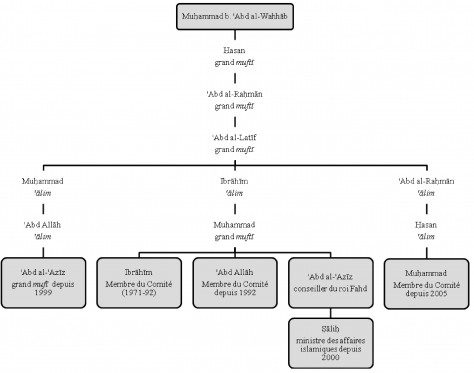
\includegraphics[width=\textwidth]{CourantsIslamContemporain/ImagesCourantsIslamContemporain/genealogie.jpeg}

13 Reste à signaler le cas particulier des oulémas originaires du Hijâz
et d'al-Aḥsā', provinces connues pour leur organisation hétéroclite. En
effet, la plupart des membres du Comité des grands oulémas, originaires
de ces régions, sont issus de ce qu'on a appelé des «dynasties»
d'oulémas, \emph{buyūtāt `ilm}, ou maisons de savoir comme ils aiment
eux-mêmes se faire appeler (à l'instar des familles d'oulémas dans les
autres pays arabes). Plus important encore est le fait que les familles
de ces oulémas appartiennent aux quatre écoles juridiques du sunnisme.
Si le facteur familial revêt une importance certaine, le paramètre de
l'origine tribale doit aussi être pris en compte.
\end{quote}

\hypertarget{la-pruxe9dominance-du-croissant-najdux12b}{%
\section{\texorpdfstring{La prédominance du croissant
\emph{najdī}}{La prédominance du croissant najdī}}\label{la-pruxe9dominance-du-croissant-najdux12b}}

\begin{quote}
14 Force est de constater que l'appartenance à une tribu, généralement
réinventée, constitue un critère identitaire important, dans une société
qui commence à peine à s'individualiser: avant d'être citoyen ou sujet,
on appartient d'abord à une tribu. C'est dire l'importance du milieu
tribal en tant que champ de socialisation des individus. La
\emph{`aṣabiyya}, l'esprit de corps tribal, joue un rôle fondamental
dans le statut social et la promotion de l'individu en Arabie Saoudite.

15 Les oulémas d'origine tribale dominent largement le Comité des grands
oulémas (il s'agit des tribus sédentarisées à partir du e siècle). Ils
sont quarante et un sur les cinquante-deux membres qu'a comptés le
Comité, depuis sa création, à être d'origine tribale, soit 79\%. Les
oulémas d'origine tribale se taillent ainsi la part du lion depuis 1971.
Les onze sièges restants sont occupés par des oulémas issus de trois
milieux différents: des membres de la notabilité citadine du Hijâz
(cooptés pour représenter les intérêts de leur région: on essaie de
choisir les plus «wahhabisés» et/ou quiétistes des oulémas du Hijâz),
des étrangers naturalisés (ils sont hanbalo-wahhabites, ont des talents
«exceptionnels» et ont défendu le hanbalo-wahhabisme et l'État) et des
citadins du Najd, sans affiliation tribale ou \emph{ḫaḍīrī}-s (ces
derniers ne doivent, en principe, leur ascension sociale qu'à leurs
compétences personnelles).

\includegraphics[width=4.9375in,height=4.20833in]{Image/media/image10.jpeg}

16 On constate alors, chiffres à l'appui, que l'appartenance au milieu
tribal sédentarisé joue un rôle déterminant dans l'ascension sociale des
oulémas, la \emph{`aṣabiyya} étant une valeur ajoutée qui permet de se
constituer un capital social. Cela dit, bien que les tribaux dominent
largement en nombre le Comité des grands oulémas, ils ne sont

toutefois pas représentatifs du paysage tribal saoudien. En effet,
certaines tribus comme les Banū Tamīm, les Banū Zayd et les Banū Ḫālid
sont «surreprésentées», tandis que d'autres comme les `Utayba n'ont
guère droit, malgré leur importance numérique, qu'à un seul représentant
au Comité des grands oulémas. D'autres tribus enfin, comme les Šammar,
les Ḥarb, les Muṭayr, les `Ajmān, les Ġāmid, etc. n'ont aucun
représentant au sein du Comité. Si la marginalisation des Šammar, des
`Utayba et des Muṭayr peut s'expliquer par leur passé de tribus
frondeuses, la marginalisation des autres tribus ne peut, elle, être due
qu'à des facteurs religieux et surtout régionaux. Nous nuancerons
seulement, pour finir, en précisant que, dans certains cas, le charisme
personnel du \emph{`ālim} -- c'est le cas d'Ibn Bāz -- fait «oublier»
son appartenance tribale. En effet, ce \emph{`ālim}, citadin sans
affiliation tribale, a pu grimper jusqu'au sommet de l'establishment
hanbalo-wahhabite (il devient grand mufti et président du Comité des
grands oulémas en 1993), uniquement grâce à son «érudition», à son
intégrité morale et à son dévouement aux Sa‛ūd. Le charisme et le
pouvoir symbolique d'Ibn Bāz ont fait de lui le plus grand \emph{`ālim}
hanbalo-wahhabite contemporain.

17 Le royaume d'Arabie Saoudite est un royaume \emph{najdī}. Les élites
saoudiennes sont majoritairement originaires de la région de Najd, fief
de la dynastie et de la doctrine hanbalo-wahhabite. Des études plus
récentes (datant de la dernière décennie) se fondent sur des données
chiffrées mais ne portent que sur les élites ministérielles, la haute
fonction publique et les membres du Conseil consultatif. Rien donc sur
les oulémas. Nous tenterons, dans ce qui suit, de combler ce manque. Sur
les cinquante- deux membres du Comité depuis sa création en 1971, 73\%
des oulémas sont originaires du Najd; 9\% du Ḥijāz, 6\% du Sud, 4\% de
la région orientale et 7\% d'origine étrangère.

\includegraphics[width=4.94996in,height=4.10417in]{Image/media/image11.jpeg}

18 Une majorité des membres du Comité des grands oulémas est donc
\emph{najdī} et ce depuis sa création. Deux remarques pourraient être
faites à ce propos. La première est que si l'on peut aisément comprendre
que seuls 4\% des grands oulémas sont des Aḥsā'ī-s puisque une grande
partie de la population de cette province est chiite ou sunnite autres
que hanbalo-wahhabite; si l'on peut aussi comprendre que seuls 9\% des
grands oulémas sont \emph{ḥijāzī} puisque, bien que sunnites, ils ne
sont, généralement, pas hanbalo- wahhabites, le chiffre de 6\% seulement
d'oulémas originaires du Sud de l'Arabie Saoudite peut, du moins \emph{a
priori}, paraître absurde puisque les habitants de cette région sont en
majorité hanbalo-wahhabites. L'hypothèse de la préférence régionale peut
être ainsi raisonnablement soutenue: si 73\% des grands oulémas sont
\emph{najdī}, c'est, justement, parce qu'ils sont originaires du fief du
hanbalo-wahhabisme et de la maison
des Sa‛ūd et que, de ce fait, leur soumission à l'un et à l'autre ne
peut être remise en cause. La seconde remarque est que si l'on compare
les chiffres avancés pour le Comité des grands oulémas à ceux que
présente le conseil des ministres au sein duquel les Najdī constituent
72\% des membres (Ibn Ṣunaytān, 2004: 70-73); à ceux du Conseil
consultatif où les Najdī sont majoritaires à 51\% (\emph{ibid}.: 93-96);
à ceux des ministres plénipotentiaires qui sont à 78\% originaires du
Najd ou encore, à ceux des hauts fonctionnaires qui comptent 67\% de
Najdī (\emph{ibid}.: 177-178), on voit que l'élite saoudienne étatique,
qu'elle soit religieuse ou politique, est majoritairement \emph{najdī}.
Les gens du Sud, eux, qui, comme on l'a dit, sont majoritairement
hanbalo-wahhabites, ne représentent que 1\% des ministres, 7\% des
membres de Conseil consultatif, moins de 5\% des ministres
plénipotentiaires et moins de 9\% des hauts fonctionnaires
(\emph{ibid}.: 177- 178): le même raisonnement peut être, ici,
développé. Le régionalisme primerait en Arabie Saoudite. Même si l'on
parle de saoudisation et de formalisation, l'État continue toujours de
s'appuyer sur l'élément najdo-wahhabite pour fonctionner.

19 Observons les chiffres de plus près: lorsque 9\% seulement des
oulémas sont originaires du Hijâz, 20\% des membres du conseil des
ministres, 29\% des membres du Conseil consultatif, 22\% des hauts
fonctionnaires sont \emph{ḥijāzī} (et 34\% parmi eux des cadres
supérieurs). Par ailleurs, en observant les chiffres de plus près
encore, il apparaît qu'au moment de la création du Comité, 29\% des
oulémas sont originaires du Hijâz contre 9\%, nous l'avons dit,
aujourd'hui. Le Comité tend donc, au fur et à mesure qu'il se met en
place et qu'il n'a plus besoin de cadres supérieurs, à se fermer à tout
ce qui n'est pas \emph{najdī}. Il faut ajouter à cela que les oulémas,
quand ils ne sont pas hanbalo- wahhabites, dissimulent leurs croyances
-- ou du moins évitent d'en parler -- et ne jouent, une fois admis au
sein du Comité, qu'un rôle de «figurants».

20 Le Comité des grands oulémas voudrait donner une illusion
d'ouverture: les principales régions sont toutes, même à une faible
proportion, «représentées». Actuellement, deux oulémas d'origine
\emph{ḥijāzi}, deux oulémas originaires du Sud et un autre de l'Est sont
membres du Comité des grands oulémas. En réalité, l'élément \emph{najdī}
domine toujours le Comité, et de loin; de plus, en supposant qu'il y ait
ouverture et même si le Comité accepte en son sein des chiites, il lui
suffirait de conserver une majorité de 51\% de hanbalo-wahhabites
(Najdī) pour que le vote à la majorité absolue passe au sein du Comité
et qu'ainsi, la vision hanbalo-wahhabite continue à dominer.

21 Enfin, en ce qui concerne les oulémas d'origine étrangère, ils ne
sont admis au sein du Comité (au nombre de trois) qu'au moment de la
création de ce Comité. Ces oulémas étrangers étaient, en effet, plus
compétents et plus qualifiés que les oulémas locaux; ils étaient dévoués
à l'État et au hanbalo-wahhabisme; nés non-wahhabites, ils l'étaient
devenus par conviction; ils n'avaient pas d'assise sociale et tribale en
Arabie Saoudite et devaient leur ascension à l'État; enfin, la
solidarité islamique, initiée par le roi Fayçal, entrait également en
ligne de compte. Depuis, le Comité s'est fermé aux étrangers et même les
enfants des dits oulémas étrangers ne sont pas admis au sein du Comité.

22 Le tracé reliant les villes du Najd dont les grands oulémas sont
originaires forme,
pour ainsi dire, un croissant que nous conviendrons d'appeler «croissant
\emph{najdī}» et qui constitue l'épicentre de l'Arabie Saoudite en même
temps que celui du hanbalo- wahhabisme. Il ne faut toutefois pas croire
que si les oulémas du Najd sont largement majoritaires au sein du
Comité, toutes les villes et les régions du Najd y seront équitablement
«représentées». Le Najd compte trois principales régions: la région de
Riyad qui a donné vingt-sept oulémas, le Qaṣīm dix et le Ḥā'il qui n'a
donné aucun \emph{`ālim}. Les deux régions, de Riyad et du Qaṣīm,
offrent un quasi-équilibre dans la répartition des oulémas: dans la
région de Riyad, en dehors de la ville elle-même, qui donne, à elle
seule, sept oulémas, les autres villes donnent, chacune, entre un et
quatre oulémas. De même, dans la région du Qaṣīm, le nombre d'oulémas
par ville varie entre un et trois.

\includegraphics[width=4.9375in,height=2.26042in]{Image/media/image12.jpeg}

23 Le Ḥā'il, quant à lui, est volontairement marginalisé pour une raison
historique évidente: l'émirat du Ḥā'il a longtemps été le rival direct
des Saoud. Nous retrouvons à peine un représentant de cette région dans
le conseil des ministres et un seul autre au Conseil consultatif (Ibn
Ṣunaytān, 2004: 71 et 94).

24 Notons, pour finir, que certaines régions du Najd sont totalement
exclues et n'ont donné aucun \emph{`ālim}: l'exemple d'al-Dawādimī, pour
ne citer que lui, explique ce phénomène dans la mesure où la plupart des
habitants de la ville sont issus de la tribu des `Utayba dont la
fidélité au régime est douteuse. Il y aurait ainsi sous-régionalisation
à l'intérieur même de la régionalisation. De même, aucun grand
\emph{`ālim} n'est issu des régions du Nord. Enfin, aucun chiite n'est
admis au Comité des grands oulémas et ce, pour des raisons évidentes
qu'il ne semble pas utile de rappeler ici. Cela dit, les acquis familial
et tribal, seuls, ne suffisent pas: l'apprenti grand \emph{`ālim} doit
encore suivre un cursus d'études particulier pour intégrer le Comité.
\end{quote}

\hypertarget{de-la-ijux101za-au-doctorat-institutionnalisation-de-la-formation-du-ux101lim}{%
\section{\texorpdfstring{De la \emph{ijāza} au doctorat,
institutionnalisation de la formation du
‛ālim}{De la ijāza au doctorat, institutionnalisation de la formation du ‛ālim}}\label{de-la-ijux101za-au-doctorat-institutionnalisation-de-la-formation-du-ux101lim}}

\begin{quote}
25 Sur les cinquante-deux oulémas qui ont été membres du Comité des
grands oulémas depuis sa création, en 1971, 22\% (soit treize oulémas)
ont reçu une formation traditionnelle et 78\% (soit trente-neuf oulémas)
une formation «moderne». Près d'un quart des oulémas sont ainsi passés
par un cursus traditionnel. Nos entretiens nous permettent de décrire ce
\emph{ta‛līm} et d'en ressortir avec le cursus traditionnel «idéal
typique» du \emph{`ālim} hanbalo-wahhabite.

26 Au départ, entre l'âge de cinq et sept ans, l'apprenti \emph{`ālim}
fait son apprentissage du Coran. Les apprentis oulémas issus d'un milieu
modeste, ceux qui seront plus tard des self-made-men, apprennent le
Coran dans une école coranique (\emph{al-kuttāb}), aux mains d'un cheikh
de renommée moyenne. Les enfants des «cadres religieux moyens» et les
rejetons des dynasties d'oulémas, eux, apprennent le Coran auprès de
leur père, de l'un des membres de leur famille, ou d'un précepteur. On
imagine bien les difficultés rencontrées par les apprentis grands
oulémas issus de milieux modestes et le décalage qui se marque, dès le
départ, entre les apprentis oulémas issus des différentes classes
sociales.

27 Après cette phase d'apprentissage du Coran, l'apprenti \emph{`ālim}
doit, d'une part, commencer à étudier la grammaire et la rhétorique
arabes, de l'autre, apprendre par cœur les trois principaux ouvrages
d'Ibn `Abd al-Wahhāb sur l'unicité divine (\emph{al- tawḥīd}),
fondements du hanbalo-wahhabisme.

28 La troisième étape du cursus classique de l'apprenti \emph{`ālim} est
la quête du savoir
auprès des oulémas réputés. Le futur grand `ālim doit, en effet, réunir
un grand nombre de \emph{ijāzāt} (pl. de \emph{ijāza}: licences), dans
toutes les branches du savoir islamique disponibles, notamment en droit
et en théologie. Il assiste, pour ce faire, plus ou moins
assidûment, à des \emph{ḥalaqāt} `\emph{ilmiyya} ou cercles de savoir,
organisés quotidiennement dans les mosquées ou aux domiciles des
oulémas. Il s'agit alors, de séances de lectures mécaniques suivies de
commentaires d'ouvrages de hadith, d'exégèse coranique, de droit et de
théologie, notamment l'étude des œuvres classiques hanbalites. C'est à
l'issue de ces \emph{ḥalaqāt}, et une fois que l'étudiant a bien retenu
l'ensemble de l'enseignement dispensé par le \emph{`ālim}, qu'il fait un
\emph{istid`ā'}: une demande d'\emph{ijāza} pour les ouvrages étudiés.
Les étudiants les plus brillants deviennent assistants du maître et cela
leur ouvre la porte pour devenir professeur ou juge: la carrière est
alors lancée. Cela a été le cas de Muḥammad al-Sbayyil, le dernier grand
\emph{`ālim} à avoir reçu une formation traditionnelle.

29 Né dans la région du Qaṣīm vers 1926, al-Sbayyil est issu d'une
famille de «cadres religieux moyens». Son père, libraire et copiste
d'ouvrages religieux, connaît parfaitement le Coran. Son frère aîné,
`Abd al-`Azīz, est un \emph{`ālim} de la ville d'al- Bukayriyya. À l'âge
de cinq ans, al-Sbayyil commence son apprentissage du Coran auprès de
son père puis de son frère. Vers l'âge de dix ans, il se lance dans
l'apprentissage des trois ouvrages fondamentaux d'Ibn `Abd al-Wahhāb. Il
étudie aussi la jurisprudence hanbalite sous la direction des oulémas du
Qaṣīm, notamment les ouvrages d'Ibn Taymiyya (m. 1328), d'Ibn Qayyim
al-Jawziyya (m. 1350) et de Mar`ī al- Karamī (m. 1624), etc. À l'âge de
vingt ans, il aurait déjà acquis plusieurs \emph{ijāzāt} qui lui
permirent de devenir l'assistant du juge du Qaṣīm, `Abd Allāh b. Ḥumayd.

30 La formation traditionnelle indispensable au tout début du e siècle
perd, peu à peu, du terrain. En effet, les oulémas qui ont reçu cette
formation s'adaptent difficilement aux exigences de la modernité. 53\%
des membres du Comité des grands oulémas, soit neuf oulémas, ont reçu,
en 1971, une formation dite traditionnelle; en 2009, aucun grand
\emph{`ālim} ne bénéficie d'une telle formation. Dans un pays qui tente
de se moderniser, le besoin d'uniformisation de la formation des grands
oulémas s'impose. Il a fallu, pour y répondre, créer un cursus complet,
homogène, un cursus «national». Nous entendons par cursus moderne, un
cursus «institutionnalisé» et uniformisé.

31 S'ils ne sont que 47\% (soit huit oulémas), en 1971, à suivre la
formation dite moderne,

ils sont aujourd'hui 100\% à le faire. Après un cycle d'études primaires
dans des écoles publiques2\emph{,} les élèves qui se destinent à faire
une carrière juridico-religieuse, rejoignent les instituts de sciences
religieuses (\emph{al-ma`āhid al-`ilmiyya}). Le premier institut voit le
jour à Riyad, en 1950, à l'instigation du grand mufti du royaume de
l'époque, Muḥammad b. Ibrāhīm. Mais très vite, le gouvernement adopte le
projet et les instituts fleurissent dans toutes les régions du royaume
pour atteindre le chiffre de soixante- deux en 2009. Pour accéder à
l'enseignement de ces instituts, l'enfant doit avoir un dossier correct
et avoir appris au moins deux parties du Coran. L'enseignement y est
gratuit. Les instituts de sciences religieuses proposent un cursus de
six années: trois années de collège sanctionnées par un certificat de
réussite, sorte de «brevet» et trois années de lycée sanctionnées par un
certificat de réussite, sorte de «baccalauréat». Les matières étudiées
ont évolué depuis les années cinquante. Au début, l'enseignement était
constitué de quatre troncs communs: les sciences religieuses, les
sciences de la langue arabe, les «sciences sociales», et les
mathématiques. Au fil des années, on a ajouté à ce tronc commun d'études
de base, l'apprentissage obligatoire de la langue anglaise et de
l'informatique. Ces instituts de sciences religieuses sont inégalement
répartis sur l'ensemble du pays: le Najd compte 34\% des instituts, le
Hijâz 13\%, le Sud 28\%, le Nord 18\%, l'Est, enfin, 7\%. Les instituts
sont nombreux dans les régions où le hanbalo-wahhabisme est majoritaire
c'est-à-dire dans le Najd, le Sud et le Nord.

\includegraphics[width=4.875in,height=3.78125in]{Image/media/image13.jpeg}

32 Si la proportion entre le nombre d'instituts créés dans le Hijâz et
celui des oulémas qui sont admis au Comité des grands oulémas est
relativement équilibrée, la proportion entre le nombre d'instituts créés
dans les trois autres régions hanbalo-wahhabites et celui des oulémas
issus de ces régions et effectivement admis au sein du Comité, est,
quant à elle, largement déséquilibrée. On s'attendrait, en effet, à un
nombre plus important d'instituts de sciences religieuses dans le Najd,
à un nombre moins important dans le Sud et à un nombre nul d'instituts
dans la région du Nord. Or, ils sont créés dans le Nord et dans le Sud
mais ce, moins dans le but de former des grands oulémas que dans celui
de «wahhabiser» ces régions en y formant des techniciens du culte
hanbalo-wahhabite et des «cadres religieux moyens».

33 Lorsque l'apprenti \emph{`ālim} a terminé avec succès ses études
secondaires au sein de l'institut, il peut postuler pour les trois
grandes universités du pays: l'Université islamique de Médine (al-Jāmi`a
al-islāmiyya), l'Université islamique de la Mecque (Jāmi`at Umm al-Qurā)
et l'Université islamique de Riyad (Jāmi`at al-imām Muḥammad b. Sa`ūd
al-islāmiyya).

34 La première de ces universités, fondée en 1961, accueille surtout les
musulmans étrangers. Les Saoudiens qui y étudient se destinent
généralement à la prédication à l'étranger. De cette université n'est
issu qu'un seul grand \emph{`ālim}.

35 Quant à la deuxième citée, elle est la plus ancienne université de
théologie d'Arabie Saoudite, fondée en 1949. Elle n'a, malgré son
ancienneté, donnée que six grands oulémas. Doit-on y voir une
manifestation du régionalisme saoudien? Toujours est-il que cette
université accueille, depuis les années soixante-dix, des professeurs,
des cadres et des étudiants de diverses tendances politico-religieuses,
notamment des frères musulmans et des sahwistes (Lacroix, 2010: 47-97)
en lesquels le gouvernement saoudien et le Comité des grands oulémas
n'ont que très peu confiance et qui ne sont donc pas spontanément
recrutés par celui-ci.

36 La dernière université, enfin, est incontestablement la plus
importante pour notre étude. Elle a donné vingt-cinq oulémas, soit 51\%
des membres du Comité, depuis sa création en 1971, et 75\% des oulémas
ayant fait des études universitaires modernes. Cette université naît, en
1974, de la fusion de la faculté de théologie créée, elle, en 1953, et
de la faculté de langue arabe, créée en 1954.

\includegraphics[width=4.95833in,height=3.34375in]{Image/media/image14.jpeg}

37 Depuis sa création, l'Université islamique de Riyad, qui,
rappelons-le, porte le nom du fondateur de l'émirat saoudien Muḥammad b.
Sa`ūd (1744-1765), fidèle allié d'Ibn `Abd al-Wahhāb, est considérée
comme le vivier des grands oulémas et de tous les cadres religieux et
techniciens du culte dont l'establishment religieux a besoin. Le

«pharaonique» campus de l'université (une véritable ville dans la ville
avec ses propres infrastructures, un petit hôpital, un supermarché, des
quartiers résidentiels pour les étudiants, les professeurs et le
personnel administratif, etc.) compte neuf facultés et deux instituts
supérieurs: la faculté de droit {[}musulman{]}; la faculté de théologie;
la faculté de langue arabe; la faculté des sciences sociales
{[}islamiques{]}; la faculté de la prédication et de la communication;
la faculté des langues et de la traduction; la faculté des sciences de
l'informatique; la faculté de l'économie; la faculté des sciences;
l'Institut supérieur de la magistrature et l'Institut de l'apprentissage
de la langue arabe {[}pour les étrangers{]}. Cela dit, les grands
oulémas sont exclusivement issus des facultés de droit et de théologie
et de l'Institut supérieur de la magistrature. Les étudiants dans ces
trois domaines bénéficient d'une bourse d'études et obtiennent, dès la
fin de leur première année d'études, le titre fort apprécié de
\emph{shaykh}. Le succès de l'Université islamique de Riyad est tel que
celle-ci s'est engagée dans une politique d'expansion en développant
deux filiales en Arabie Saoudite3 et cinq à l'étranger4\emph{.} Enfin,
certains étudiants peuvent préparer leur doctorat en sciences
religieuses à l'université égyptienne d'al-Azhar, pour le prestige que
cela donne. Une autre raison pourrait être avancée: certains apprentis
oulémas saoudiens iraient à al-Azhar pour observer l'organisation, les
structures et les mécanismes de fonctionnement de cette prestigieuse
université en vue de les
«importer» en Arabie Saoudite.

38 Les oulémas, au moment de leurs études supérieures, ont tous un tronc
commun tripartite: les fondements de la théologie (\emph{al-`aqīda});
l'exégèse coranique (\emph{al tafsīr}) et la jurisprudence
(\emph{al-fiqh}). À partir de la première année de master (calqué sur le
système anglo-saxon), 74\% des oulémas se spécialisent dans la
jurisprudence, et plus spécialement dans les fondements de la
jurisprudence islamique (\emph{uṣūl al-fiqh}) dans le but d'acquérir la
qualification requise pour émettre des \emph{fatwā}; 26\% d'entre eux,
se spécialisent en théologie, et plus précisément en religions comparées
(en réalité, pour dénigrer toute autre religion que l'islam
hanbalo-wahhabite)5\emph{.} Le choix de ces spécialisations n'est pas
étonnant dans la mesure où les étudiants se destinent avant tout à être
des techniciens du culte et des gestionnaires des biens de salut. Nous
n'entrerons pas, pour ne pas alourdir notre propos, dans le détail des
spécialisations pointues à l'intérieur même des deux grands domaines de
spécialisations que nous avons évoqués.

39 Bien que le cursus moderne se soit bien implanté dans le paysage
saoudien, l'ijāza
n'en demeure pas moins source de prestige et un élément non négligeable
dans un
capital social. Nous avons pu observer que la totalité des oulémas qui
ont suivi le cursus moderne ont, néanmoins, obtenu une ou plusieurs
\emph{ijāzāt}. Elément de prestige comme nous venons de le dire,
l'\emph{ijāza} est, en théorie, facultative. Mais, en pratique,
l'obtention d'une \emph{ijāza} permet au \emph{`ālim}, d'une part, de se
rattacher à une chaîne de transmission
«ininterrompue» d'oulémas remontant jusqu'au Prophète, ce qui permet au
\emph{`ālim} de légitimer sa position et son savoir et de s'inscrire
dans l'héritage prophétique, d'autre part, de nouer des relations
privilégiées avec un ou plusieurs oulémas et de commencer ainsi à tisser
un réseau qui pourra le mener au sommet de l'establishment hanbalo-
wahhabite.

\textbf{Faire carrière: le \emph{cursus honorum} des oulémas}

\includegraphics[width=4.97917in,height=3.92708in]{Image/media/image15.jpeg}40
L'enseignement et la magistrature ont toujours été les métiers de
prédilection des oulémas. Les membres du Comité des grands oulémas
n'échappent pas à cette règle. 96\% d'entre eux exercent au moins une de
ces deux professions: 50\% du Comité, soit vingt et un grands oulémas,
ont été ou sont encore, professeurs de jurisprudence islamique ou de
théologie; 31\% d'entre eux sont magistrats dans les différentes
instances de la justice saoudienne; 15\% des grands oulémas ont cumulé
les deux fonctions. À la question: «pourquoi le choix de ces métiers?»
Une première réponse, unanime, des grands oulémas magistrats: «la
justice est le fondement de la royauté». Et, selon les oulémas, qui,
mieux que des spécialistes de «la loi divine», pourraient mettre la
justice en application! Les grands oulémas ont d'ailleurs pleine
conscience de l'importance de leur mission. Ils ont une vision
catastrophiste d'un monde où le \emph{`ilm}, qui risque d'être perdu,
doit être sauvé, épuré des innovations blâmables et transmis par le
\emph{`ālim}.

41 En outre, si la magistrature permet au grand \emph{`ālim} d'observer,
d'analyser et de statuer sur des cas concrets, l'enseignement permet de
transmettre le savoir théorique. Cela, en plus du prestige qui entoure
ces deux fonctions. Il n'est, enfin, pas étonnant de voir que nombre de
grands oulémas cumulent les deux fonctions puisqu'en réalité, l'une et
l'autre sont indissociables (pratique et théorie). Ce phénomène de cumul
des fonctions (d'enseignant et de magistrat) est surtout visible dans la
première génération des grands oulémas. Il s'explique par le manque de
cadres religieux au moment de la
création du Comité. Les grands oulémas devaient donc assumer, tout à la
fois, leur rôle au sein du Comité et les fonctions de magistrats et
d'enseignants. Des années quarante aux années soixante, l'Arabie
Saoudite a été obligée d'«importer» des cadres religieux de l'étranger,
notamment de l'Égypte. Un exemple: l'Égyptien `Abd al-Razzāq `Afīfī (m.
1994), arrivé en Arabie Saoudite, en 1949, pour enseigner la langue
arabe et les sciences religieuses dans un collège à Tayef, a gravi, un à
un, les échelons et parvient au sommet de l'establishment religieux: il
est nommé, en 1971, au sein du Comité des grands oulémas. Cet exemple
révèle deux réalités: premièrement, l'Arabie Saoudite a fait appel aux
étrangers pour l'enseignement, à une certaine époque, à cause du déficit
de cadres dont elle a souffert dans tous les domaines; et deuxièmement,
les étrangers hanbalo-wahhabites, qui pouvaient aisément s'intégrer dans
le pays d'accueil, ont pu, à force de persévérance, atteindre le sommet
de l'establishment religieux saoudien.

42 La pratique du cumul des fonctions d'enseignant et de magistrat tend
à disparaître: le dernier grand \emph{`ālim} à avoir cumulé ces deux
fonctions est `Abd Allāh b. Qa`ūd, membre du Comité de 1977 à
19866\emph{.} Désormais, les grands oulémas, qu'ils soient professeurs
ou magistrats, sont de plus en plus spécialisés, chacun dans son
domaine: de professeurs de droit en général, ils sont devenus
professeurs de droit pénal, de droit de la famille, etc. Parallèlement à
ces deux métiers de prédilection, les grands oulémas sont techniciens du
culte: la plupart d'entre eux sont imâm dans les mosquées. Par exemple,
le grand mufti actuel du royaume, `Abd al-`Azīz āl al-Shaykh, est
également imâm de la grande mosquée de Riyad. Sāliḥ b. Ḥumayd est, lui,
imâm de la grande mosquée de la Mecque, etc. N'oublions pas enfin,
l'autre fonction essentielle des grands oulémas, celle d'«entrepreneurs»
de biens de salut, à savoir promulguer des \emph{fatwā} et se mettre à
l'écoute de la population. Mais si les grands oulémas monopolisent les
grands postes religieux et judiciaires saoudiens, ils n'hésitent pas à
empiéter sur le domaine réservé des autres élites.

43 Une fois admis au sein du Comité, le grand \emph{`ālim} obtient
automatiquement le grade de haut fonctionnaire (\emph{al-martaba
al-mumtāza}), voire celui de ministre. Sur les cinquante-deux membres du
Comité des grands oulémas, vingt-deux ont occupé des postes de
responsabilité autres que ceux de magistrats et d'enseignants. Déjà neuf
membres de la \emph{Hay'a} ont été ou sont encore ministres. Les
ministères que contrôlent les oulémas (si ce ne sont pas eux qui les
contrôlent directement, c'est un membre de l'establishment religieux)
sont ceux de la justice, des affaires islamiques, du pèlerinage et de
l'enseignement des filles (avant le rattachement de ce dernier, en 2002,
au ministère de l'éducation nationale). Depuis sa création, le ministère
de la justice est dirigé par un membre du Comité7\emph{.} Huit membres
du Comité des grands oulémas on été membres du Conseil consultatif: le
président de ce conseil, qui fait se côtoyer islamistes,
«libéraux», conservateurs et tribaux, depuis sa création, en 1992, est
un membre du Comité des grands oulémas. De 1992 à 2002, c'est Muḥammad
b. Jubayr, membre du Comité des grands oulémas (de 1971 à 2002), qui
assure la présidence de cette instance. Sāliḥ b. Ḥumayd, membre du
Comité des grands oulémas depuis 2001, lui succède en 2002. Ce dernier
est remplacé par `Abd Allāh Āl al-Shaykh, en 2009. Trois membres de la
\emph{Hay'a} ont été conseillers du roi Fahd (1982-2005) et deux sont
actuellement conseillers du roi `Abd Allāh. Quatre membres du Comité ont
occupé les postes de doyen ou de président d'université. Par exemple,
`Abd al-`Azīz b. Bāz occupe jusqu'à sa mort, en 1999, le poste de
président de l'Université islamique de Médine. Sa`d al- Ḍuwayḥī est
doyen de la faculté de théologie d'al-Aḥsā'. `Abd Allāh b. `Abd
al-Muḥsin al- Turkī, sans doute l'un des membres les plus actifs du
Comité, actuellement, occupe le poste de président de la Ligue islamique
mondiale, après avoir occupé, entre autres, les postes de président de
l'Université de Riyad et de ministre des affaires islamiques.

44 C'est dire que les oulémas ont adopté, depuis au moins deux
décennies, une stratégie adaptative qui les pousse à investir plusieurs
secteurs d'activités. Outre les domaines religieux, législatif et
éducatif, ils investissent les associations caritatives, les
organisations gouvernementales et non gouvernementales et les domaines
économique et financier. Dans ces deux derniers domaines, trois oulémas,
`Abd Allāh b. Manī`, `Abd
al-Wahhāb Abu Sulaymān et `Abd Allāh al-Muṭlaq se sont «improvisés»
experts et consultants incontournables dans les marchés financiers
saoudiens. Les trois hommes sont aussi membres de plusieurs conseils
d'administration de banques et d'entreprises dans le cadre de ce que
l'on appelle en Arabie Saoudite \emph{al-lijān al-šar`iyya} ou
commissions islamiques. Le nom-même d'un grand \emph{`ālim} sur la
brochure d'une société ou d'une entreprise est la meilleure des
publicités.
\end{quote}

\hypertarget{la-multiplication-des-ruxe9seaux-de-soutien}{%
\section{La multiplication des réseaux de
soutien}\label{la-multiplication-des-ruxe9seaux-de-soutien}}

\begin{quote}
45 Cette mobilité des oulémas n'est, toutefois, possible que si le
\emph{`ālim} tisse, autour de lui, un réseau sur lequel il peut
s'appuyer. Les capitaux culturel et économique doivent encore être
complétés par un réseau de soutiens. Nous avons pu observer trois types
de capitaux sociaux mobilisés par le futur grand \emph{`ālim}. Autrement
dit, le recours aux relations personnelles permet à ce dernier de
s'assurer une meilleure position dans la hiérarchie sociale. Ces trois
réseaux, que nous exposons séparément, sont en réalité, presque
toujours, combinés par le futur grand \emph{`ālim}. Le réseau familial
constitue la première ressource du futur grand \emph{`ālim}. Nous avons,
en effet, constaté l'existence d'au moins trois exemples de réseaux
familiaux qui sont autant de moyens d'accès au Comité des grands
oulémas.

46 Le premier est, sans aucun doute, le plus puissant et le plus dense:
celui des Āl al- Shaykh. Nous avons évoqué plus haut l'importance de
cette famille et nous tenterons, dans ce qui suit, de compléter le
tableau amorcé. L'exemple des deux fils, Ibrāhīm et `Abd Allāh, du grand
mufti Muḥammad b. Ibrāhīm est tout à fait significatif: bien que le
premier des deux ait été relativement peu brillant par rapport aux
collaborateurs de son père, il a quand même été nommé par ce dernier
vice-mufti du royaume d'Arabie Saoudite. Après la mort de son père et la
suppression du poste de mufti, Ibrāhīm, qui était destiné à devenir
mufti, reçoit, en guise de consolation, les postes de ministre de la
justice, de membre du Comité des grands oulémas et de président de la
Direction de la recherche scientifique, de la prédication et de
l'instruction! En 1992, lorsqu'Ibrāhīm se retire des affaires, son
remplaçant au ministère et au Comité des grands oulémas n'est autre que
son frère cadet `Abd Allāh, président actuel du Conseil consultatif. Un
autre exemple étonnant de la famille Āl al-Shaykh: il s'agit de Ṣāliḥ b.
'Abd al-`Azīz, le petit fils d'Ibn Ibrāhīm. Après avoir fait des études
scientifiques depuis le lycée et obtenu un diplôme d'ingénieur, Ṣāliḥ
décide de récupérer l'héritage familial et s'inscrit à l'Université
islamique de Riyad. Grâce à son nom et à l'intervention de son père, qui
était l'un des conseillers du roi Fahd, il obtient une équivalence et
passe ainsi directement en année de master: il contourne la règle qui,
aussi stricte soit-elle, s'efface quand il s'agit d'un Āl al-Shaykh. Il
est actuellement ministre des affaires islamiques et, potentiellement,
membre du Comité des grands oulémas. Un dernier exemple enfin de cette
famille: le dernier admis à Hay'at kibār al-'ulamā', Muḥammad b. Ḥasan,
fait une ascension fulgurante grâce à ses bonnes relations avec son
cousin, le grand mufti actuel d'Arabie Saoudite: il a pu, rapidement,
gravir les échelons universitaires et devenir le directeur de cabinet du
mufti. Ce dernier l'épaule et le soutient: il propose son nom au Comité
des grands oulémas auquel Muḥammad b. Ḥasan accède en avril 2005.
Signalons, enfin, que le réseau familial des Āl al-Shaykh et l'influence
qui en découle, dépassent largement le seul cadre religieux: un membre
de la famille est ambassadeur à Paris, un autre est directeur du
protocole royal, un troisième est membre de la chambre de commerce, etc.
Le deuxième réseau familial est celui des Ibn Ḥumayd, déjà présenté plus
haut.

47 Le dernier réseau familial, enfin, de moindre importance, est celui
des al-Šathrī: cette
famille du Najd a donné quelques oulémas et plusieurs hommes politiques.
`Abd al-‛Azīz al-Šathrī, un des conseillers des rois Fayçal (1964-75) et
Ḫālid (1975-82) a également été un ouléma de renommée moyenne. Son fils,
Nāṣir, a réussi à faire une brillante carrière politique (en tant que
conseiller des rois Ḫālid et Fahd). Selon un des
membres du clan al-Šathrī: «il ne manquait à {[}la{]} famille qu'un
grand \emph{`ālim} pour qu'{[}elle{]} devienne, enfin, une grande
famille». La parentèle met tout en œuvre pour que son rejeton prodige,
Sa‛d, accède au sommet de l'establishment religieux. Aussi, le
prépare-t-on, dès son plus jeune âge, à devenir grand \emph{`ālim} : on
le confie aux maîtres les plus compétents dans le domaine, tels Ibn Bāz,
Ibn `Uthaymīn, al-Aṭram, al-Rakbān et `Abd al-`Azīz Āl al-Shaykh. On le
pousse à s'inscrire à Jāmi'at al-imām où il obtient un doctorat en
fondements de la jurisprudence islamique. Sa`d brûle toutes les étapes
du \emph{cursus honorum} hanbalo-wahhabite et devient professeur de la
même université en un temps records. En mars 2005, la famille soutient
la candidature de son fils au Comité des grands oulémas (le père est
membre du cabinet royal qui transmet les candidatures au roi). Sa`d est
finalement nommé, en avril 2005: à trente-huit ans, il est le plus jeune
membre de l'histoire du Comité des grands oulémas.

48 Nous l'avons dit, le régionalisme et le segmentarisme dominent le
paysage politico- religieux saoudien. La deuxième ressource du futur
grand \emph{`ālim} est, naturellement, le réseau tribal qui va de pair
avec le réseau régional, autrement dit avec le réseau \emph{najdī}. Nous
avons remarqué, en analysant les origines géographiques et tribales des
grands oulémas, que ces derniers sont généralement issus des plus
grandes confédérations tribales du Najd: les Banū Ḫālid ont donné quatre
grands oulémas, les Banū Zayd, sept, les Banū Subay`, trois, les Banū
Tamīm, huit (auxquels il faut ajouter les quatre grands oulémas des Āl
al-Shaykh), les Qaḥṭān, trois, les `Unayza, trois, les Bāhila, deux et
al- Dawāsir, deux également. Soit un total de trente-six grands oulémas
issus des grandes tribus du Najd sur les cinquante-deux membres du
Comité. Le réseau tribal est très dense. Le nombre de grands oulémas est
plus ou moins bien réparti entre les grandes tribus \emph{najdī}. D'un
mouvement de nomination au sein du Comité à l'autre, cet équilibre est,
consciemment ou inconsciemment, maintenu. Exemple: les deux grands
oulémas, Muḥammad āl Sulaymān et Bakr Abū Zayd, de la tribu des Banū
Zayd -- admis tous deux au Comité, en 1992 -- sont remplacés, en 2005,
par deux hommes issus de la même tribu, `Alī al-Ḍuwayḥī et `Abd
al-Raḥmān al-Sadḥān. D'ailleurs, le réseau tribal doublé du réseau
régional ne concerne pas uniquement le champ religieux: on retrouve ces
mêmes configurations dans le domaine politico-administratif (Ibn
Ṣunaytān, 2004, 59-62).

49 La dernière ressource du futur grand \emph{`ālim} est la
\emph{mulāzama}: le fait de s'attacher un
long moment à un maître en sciences religieuses, réputé et influent.
Côtoyer un maître pendant plusieurs années permet à l'apprenti grand
\emph{`ālim} de nouer avec lui des relations personnelles qui peuvent
même aboutir au mariage de l'élève avec la fille ou la nièce du maître.
Par exemple, Ṣāliḥ al-Luḥaydān est, pendant plusieurs années, le
disciple favori du grand mufti Muḥammad b. Ibrāhīm. Cette relation
privilégiée lance véritablement la carrière de Ṣāliḥ qui devient le
gendre et le directeur de cabinet du mufti et qui gagne peu en peu en
charisme. Une année seulement après le décès du maître, al-Luḥaydān est
admis au Comité des grands oulémas; il hérite aussi de la fonction de
magistrat; quelques années plus tard, il devient le président du Haut
conseil de la magistrature, poste qu'il occupe jusqu'en février 2009.
Al-Luḥaydān est le doyen du Comité des grands oulémas dont il est membre
depuis 1971. Il en est aussi un des membres les plus influents. Il
serait, en effet, le seul à pouvoir opposer un veto pour la nomination
d'un nouveau membre: en 2005, il aurait utilisé son veto pour s'opposer
à l'entrée de l'ouléma `Abd al-Muḥsin al-`Ubaykān au Comité.

50 Un autre exemple: Muḥammad al-Sbayyil est le disciple d'Ibn Ḥumayd
alors que
celui-ci est le \emph{qāḍī} d'al-Bukayriyya. Quand Ibn Ḥumayd devient le
\emph{qāḍī} du Qaṣīm, il fait appeler al-Sbayyil à Burayda pour le
désigner professeur et responsable d'un institut de sciences religieuses
de la région. La relation entre les deux hommes est telle que,
lorsqu'Ibn Ḥumayd devient le grand juge du Ḥijāz, il le fait venir à la
Mecque et le nomme imâm de la grande mosquée de la Mecque et
vice-président de l'administration chargée de gérer les deux lieux
saints. Il finit même par en devenir président (jusqu'en 2005) après la
disparition de son protecteur. Depuis son arrivée à la Mecque, il tisse
des
relations étroites avec des oulémas et grands oulémas notamment Ibn Bāz
(qui n'est pas son maître) mais qui finit par lui proposer de devenir
membre du Comité en 1992.

51 Un troisième exemple: c'est également Ibn Bāz qui suit, pas à pas, la
carrière de `Abd
Allāh b. Qa'ūd qui est son meilleur disciple. À la première occasion (le
décès d'Ibn Ḥumayd et de Miḥḍār `Aqīl), Ibn Bāz propose le nom d'Ibn
Qa`ūd au cabinet royal qui le nomme membre du Comité en 1977.

52 Un dernier exemple enfin: le mufti actuel, `Abd al-`Azīz āl
al-Shaykh, en plus du réseau familial que lui confère son nom, bénéficie
du soutien de son maître Ibn Bāz. Il s'agit d'abord d'une question de
solidarité et de reconnaissance: Ibn Bāz est un \emph{mulāzim} du grand
père de `Abd al-`Azīz Āl al-Shaykh, Muḥammad b. `Abd al-Laṭīf. Il aide
donc `Abd al-`Azīz Āl al-Shaykh à devenir professeur à l'université
d'al-Imām, et propose son nom au cabinet royal pour en faire un membre
du Comité des grands oulémas (il le deviendra en 1987). En 1993, Ibn Bāz
devient mufti et désigne `Abd al-`Azīz āl al-Shaykh vice-mufti du
royaume et ce, bien que d'autres grands oulémas soient plus compétents
que lui. En effet, depuis les années soixante et jusqu'à sa mort, en
1999, Ibn Bāz occupe une position-clé dans l'establishment religieux. Il
bénéficie du respect et de la considération des autres grands oulémas et
exerce, de ce fait, une influence autour de lui, tous les grands oulémas
tenant compte de ses conseils et suivant à la lettre ses directives. La
centralité d'Ibn Bāz est ainsi très importante: un grand nombre de
chemins passent par lui. Dix-huit grands oulémas sont ses disciples et
certains d'entre eux lui doivent leur entrée au sein du Comité.
\end{quote}

\hypertarget{le-quiuxe9tisme-politique}{%
\section{Le quiétisme politique}\label{le-quiuxe9tisme-politique}}

\begin{quote}
53 En cherchant à identifier les conditions d'accès au Comité des grands
oulémas à travers le parcours de ses membres, nous avons constaté qu'il
existe deux critères directement liés à la vie politique et sociale:
aucun des grands oulémas n'a de passé politique (c'est-à-dire, une
quelconque manifestation d'opposition au régime: demande de réformes, ou
autres), et aucun \emph{`ālim} n'a jamais critiqué les décisions du
Comité ou de l'un de ses membres et ce, même si ses positions allaient à
l'encontre des décisions officielles.

54 `Abd Allāh Ibn Jibrīn, haut fonctionnaire religieux et candidat
potentiel au Comité des grands oulémas, a été l'un des parrains de la
contestation islamiste des débuts des années quatre-vingt-dix (Kepel,
2003: 335-337; Lacroix, 2007: 371-443). Ces actes constituent une
véritable offense tant pour le régime que pour les grands oulémas. Ces
derniers ne manquent pas, d'ailleurs, de le désavouer publiquement: il
est démis de ses fonctions officielles. Réhabilité par la suite, et bien
que très bon \emph{`ālim}, il ne pourra cependant jamais prétendre au
poste de grand \emph{`ālim} en raison de cette «bavure»: s'étant
ouvertement opposé au gouvernement et ayant participé à des activités
politiques allant à l'encontre des positions officielles, son «rachat»
et son récent soutien au gouvernement ne suffisent pas. Il ressort de
cet exemple que le quiétisme politique des candidats au Comité est un
élément fondamental et un critère-clé de sélection. Tout ce que peut
tolérer le Comité comme engagement politique pour un futur grand
\emph{`ālim} est le soutien aux décisions du pouvoir. `Alī al-Ḍuwayḥī
est l'exemple du \emph{`ālim} engagé politiquement -- en faveur du
régime bien sûr -- qui accède à la Hay'a. En effet, depuis 2001,
al-Ḍuwayḥī, qui dirige la faculté de théologie d'al-Aḥsā', a signé
plusieurs pétitions politiques défendant les programmes scolaires
saoudiens, et se déclarant en faveur de la tenue d'élections
municipales, etc.

55 Quant à `Abd al-Muḥsin al-`Ubaykān, qui a appelé ouvertement le
gouvernement à entreprendre des réformes, entre 1992 et 1994, il a été
marginalisé et démis de ses multiples fonctions: il perd son poste de
juge au tribunal de Riyad et d'imâm de mosquée. Réhabilité, dans les
années 1999-2000, il continue néanmoins à critiquer les décisions de la
Hay'a (surtout celles qui concernent la jurisprudence), et du système
judiciaire. Il émet même des \emph{fatwā} contredisant celles du Comité
des grands oulémas et
tente, pour se rattraper, de promulguer des \emph{fatwā} sur la licéité
du salut du drapeau national, sur la condamnation des sahwistes ou
encore sur l'interdiction du djihâd en Irak pour les Saoudiens. Le
gouvernement a accepté de le réhabiliter mais les oulémas ont opposé un
veto catégorique à l'entrée de ce \emph{`ālim} au Comité. Al-`Ubaykān a,
finalement, été nommé, dans un premier temps, conseiller au ministère de
la justice et membre du Conseil consultatif, avant de devenir l'un des
conseillers du roi, en 2009.

56 Les leaders de la \emph{ṣaḥwa} dans les années quatre-vingt-dix,
Safar al-Ḥawālī, Salmān al-`Awda et Muḥsin al-`Awājī, reconnaissent
eux-mêmes que l'un des critères d'accès au Comité des grands oulémas est
le quiétisme sur les plans politique et sécuritaire et acceptent donc,
du fait de leur très grand engagement politique, de ne pas y prétendre.

«Pour le gouvernement, dit al-Ḥawālī, les grands oulémas doivent être
des hommes apolitiques, des hommes qui ignorent tout de la politique».
Salmān al-`Awda ajoute que

«les futurs membres du Comité doivent être des hommes sans histoire(s)».
Pour Muḥsin al-`Awājī «l'accès au Comité obéit à des critères purement
sécuritaires».

57 Il découle de tout cela le «portrait idéal» du membre du Comité des
grands oulémas:

le grand \emph{`ālim} est hanbalo-wahhabite; il est issu d'une famille
de «cadres religieux moyens» ou d'une «dynastie» d'oulémas; il est issu
d'une grande tribu sédentarisée du croissant \emph{najdī}; il a effectué
des études auprès de maîtres réputés (cela pour le \emph{`ālim} qui suit
une formation traditionnelle) ou dans un \emph{ma`had `ilmī} puis à
l'université al-Imām de Riyad (pour le grand \emph{`ālim} qui a reçu une
formation moderne); il s'est spécialisé en jurisprudence islamique; il
est généralement professeur d'université (al-Imām) ou magistrat; il a en
moyenne vingt-cinq années d'expérience dans le domaine religieux; il
n'est pas engagé politiquement (s'il l'est, il ne doit l'être qu'en
faveur du régime).

58 La moyenne d'âge du grand \emph{`ālim} qui accède au Comité est de
quarante-sept ans. Il y reste en moyenne quinze ans. Et, si les
circonstances d'accès à la Hay'a sont difficiles à déterminer, les
circonstances de départ de la Hay'a sont, elles, tout à fait claires: le
grand \emph{`ālim} quitte le Comité s'il décède, bien évidemment, s'il
est gravement malade ou s'il a commis un acte jugé répréhensible par le
roi -- en 1992, quatre grands oulémas auraient refusé de signer une
\emph{fatwā} et ont été limogés.

59 Le renouvellement des membres du Comité des grands oulémas est
généralement associé à une période de crise ou de transition. Les
renouvellements de 1987 et de 2001 sont des renouvellements de
transition (plusieurs oulémas sont décédés ou gravement malades), les
renouvellements de 1992 et 2005 coïncident avec des moments de crise
(respectivement, les conséquences de la guerre du Golfe et celles du 11
septembre). Depuis la création de la Hay'a, il y a eu reproduction de
l'élite: il ne reste plus de la génération de 1971 que trois membres.
Nous constatons toutefois que l'élite des grands oulémas restreint
l'accès, même à des personnes qui rempliraient toutes les conditions
formelles pour accéder au Comité. Sans doute le prestige d'appartenir au
Comité des grands oulémas ne pourrait que diminuer si l'accès devenait
trop aisé. L'élite du Comité est donc fermée: cinquante-deux membres en
trente-huit ans.
\end{quote}

\hypertarget{conclusion}{%
\section{Conclusion}\label{conclusion}}

\begin{quote}
60 L'habitus, ainsi défini, des grands oulémas, fruit d'un
conditionnement historique et social, est générateur d'un comportement
adapté, consciemment ou inconsciemment, à la logique de l'espace
politico-religieux saoudien: soutenir le pouvoir politique et gérer le
marché officiel des biens de salut. Les larges prérogatives dont dispose
le Comité dans les domaines politique, social et religieux, à côté de sa
fonction fondamentale de bastion idéologique et d'usine à légitimer les
actions du gouvernement, justifient le contrôle par le pouvoir politique
de son ordre du jour et de son budget et conditionnent le choix, très
sélectif, de ses membres. Les grands oulémas, qui se définissent eux-
mêmes comme les oulémas du pouvoir, doivent être acquis au régime. Si
les origines sociales, le parcours éducatif et les réseaux de
socialisation favorisent l'émergence d'une élite fermée et dévouée au
pouvoir, la `\emph{aṣabiyya} régionale y est pour beaucoup. Le

Comité est, à l'instar des autres institutions du pays, trusté par
l'élément \emph{najdī} (plus de 70\% des membres des élites saoudiennes
sont \emph{najdī}): cette région n'est-elle pas le fief du
hanbalo-wahhabisme et de la dynastie régnante? Il s'agit enfin pour les
oulémas d'un dévouement objectif: les intérêts spirituels et temporels
de l'establishment religieux étant intrinsèquement liés à ceux du
régime, si ce dernier était mis à mal, la domination du
hanbalo-wahhabisme sur le territoire saoudien -- très éclectique
religieusement -- serait indubitablement remise en cause.
\end{quote}


\chapter{Le mouvement réformiste (fin XIXe - début XXe)}
  \mn{(07/02/2022)}
 
 
  
  `ABDUH Muhammad, \emph{Rissalat ai Tawhid - Exposé de la religion
  musulmane}, Geuthner, Paris, 1925, trad. fr. et introduction B. Michel
  et Ch. Moustapha Abdel Razik.
  
 
  
  AL-AFGHANI Jamâl ad-Din, \emph{La réfutation des matérialistes},
  Geuthner, Paris, 1942, trad. fr. A.-M. Goichon. Textes divers in:
  \emph{Orient}, 1962, N° 21 p. 89-115, N°22 p. 125-160, N° 23 p. 169-
  198, N' 24 p. 125-152 et \emph{Orient}, 1963, N° 25 p. 141-152.
 


HADDAD, Mohammed \emph{Le réformisme musulman : une histoire critique},
Paris, Mimesis, 2013. HOURANI, Albert \emph{La pensée arabe et
l'Occident,} Groupe Naufal Europe, Paris, 1991.

JOMIER Jacques \emph{Le Commentaire coranique du Manâr}, Maisonneuve,
Paris, 1954.

MERAD Ali \emph{Le réformisme musulman en Algérie de 1925 à 1940. Essai
d'histoire religieuse et sociale}, Paris, Mouton et Cie, 1967.
 \emph{Ibn Bâdis,
commentateur du Coran}, Geuthner, Paris, 1971.

METCALF, Barbara \emph{Islamic Revival in British India 1860-1900},
Princeton University Press, 1982.

TROLL, Christian \emph{Sayyid Ahmad Khân. A Reinterpretation of Muslim
Theology}, Vikas Publ.

House, New Delhi, 1978.



 \section{Introduction : Arrière fond positiviste}
 
 \paragraph{Auguste Comte}
 
 \paragraph{idée de progrès} Évolutionnisme de société. Le progrès est porté par l'occident. Vision des sociétés évoluant vers un mieux, du coup, hiérarchisation des sociétés, entre les sociétés archaïques et celles qui s'appuient sur la Raison et ont dépassé le stade de la religion.
 
 \paragraph{Acceptation des valeurs occidentales} souveraineté du peuple; droits individuels; liberté d'expression. 
 
 \paragraph{Un discours critique de la Religion} 
 
  %-----------------------------------------------------------------------------------
  \section{Les « Occidentalisants »}
  
\paragraph{trois premiers quarts du XIX} jeunes de l'élite de l'empire Ottoman. L'empire cherche à se réformer en introduisant des éléments européeans. L'Empire Ottoman envoie des jeunes en France pour se former.

\paragraph{Tahtawi} Egyptien, a vécu 5 ans en France (1826-1831). A été ensuite dans l'administration ottomane. \textit{L'Or de Paris}\sn{très intéressant à lire}

\paragraph{Khayr ad-din} Caucasien, installé en Tunisie. A vécu à Paris (1852-1856).

\paragraph{Jeunes ottomans} dans le contexte turque. 

\paragraph{Ils notent le désir de progrès} A la différence de Al Wahhab qui est soupçonneux de l'\textit{innovation}, on valorise le changement social : 
\begin{quote}
    quiconque maitrise un art désire inventer quelque chose inconnu auparavant \sn{Or de Paris}
\end{quote}

 
 \paragraph{État}  Sur le plan politique, une compréhension différente de l'État. Dans le cadre classique, l'État doit assurer la justice. Or, ici l'État encadre le progrès de la société. Ils sont convaincus que ce sont les institutions politiques qui sont à l'origine de la force des États occidentaux. Par contre, ils vont être en retrait sur l'approche critique de la religion du positivisme.
 
 \paragraph{les lumières ont émancipé l'Europe de l'obscurantisme chrétien} avec une pointe polémique : les lumières viennent de la philosophie musulmane, et donc adopter les lumières pour les musulmans, ce n'est pas trahir le patrimoine musulman, c'est se le réapproprier. \sn{C'est la pointe de Tariq Ramadan dans les années 1990}.
 
 \paragraph{Principes politiques} Ils vont associer les principes démocratiques au principe de la \emph{Shura}, \textit{consultation}, principe coranique de consultation des notables, reinterprété dans un contexte moderne.
 \begin{Def}[shura]
    \emph{ intention} - consultation
\end{Def} 
 \paragraph{droit musulman} dans un cadre musulman, Il faut moderniser le droit musulman pour qu'il puisse accompagner le développement de la société. Ils pronent une unification du droit, une seule école, moderne et uniforme. Il faut viser à l'éducation des jurisconsultes, dans un cadre moderne. 
  
  %-----------------------------------------------------------------------------------
  \section{Trois grands réformistes}
   
   Après les occidentalisants, qui préfigurent les modernistes, il y a les réformistes que l'on verra à travers trois figures.
   
   \paragraph{Seyyed Ahmad Khan (1817-1898)} Il ne sort pas de nul part, son père est soufi et sa mère a été formé dans une école fondé par Walî Allâh (P \pageref{Theo:waliAllah}). Très grande figure en Inde
   
   \paragraph{Jamal ad-din Al Afghani (1839-1897)} formé en Inde mais action dans l'Empire Ottoman (séjour important en Egypte (1871-79)) et un autre à Paris où il est exilé (1881-1883). C'est un activiste  : revues, société secrète. Son but est de lutter contre la colonisation. Il finit sa vie sous surveillance ottomane.
   

  
   
    \paragraph{Muhammad Abduh} Egyptien, successeur d'Al Afghani. Il a ensuite développé sa propre pensée. 
    \begin{marginfigure}
       \centering
       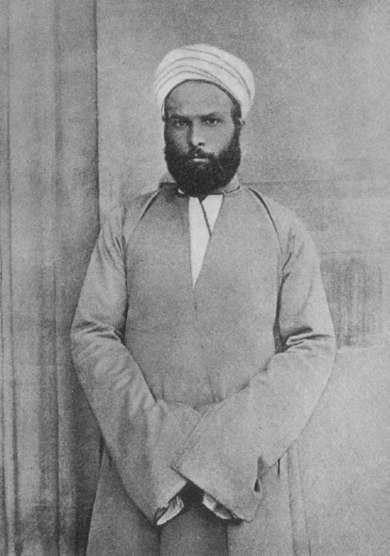
\includegraphics[width=.7\textwidth]{CourantsIslamContemporain/ImagesCourantsIslamContemporain/390px-Muhammad_Abduh.jpg}
       \caption{\href{https://fr.wikipedia.org/wiki/Mohamed\_Abduh}{Muhammad Abduh}}
       \label{fig:my_label}
   \end{marginfigure}
   Surtout en Egypte mais a partagé le séjour parisien de \textit{Aghani} puis au Liban. On lui a interdit d'enseigner mais il a été nommé grand mufti d'Egypte (1899). On avait moins peur de son activité du droit que de son activité sur les jeunes en tant qu'enseignant. Fonde aussi une école qui va évoluer différemment.  
    
    \paragraph{Avancée coloniale plus avancée} La colonisation s'est accentuée : les occidentaux apparaissent comme une menace politique. Peur du colonialisme. Le positivisme s'est aussi accentué. Ils doivent se situer dans le rapport entre Foi et Raison. 
   
   \paragraph{Héritiers du pre-réformisme} En inde en particulier, décadence du monde musulman. beaucoup plus faibles que l'occident, parce que \textit{nous avons perdu l'authenticité de la Foi musulmane}. Pour retrouver notre puissance, il faut retrouver l'authenticité de la pratique et la Foi musulmane.
   
   \paragraph{Mais des différences} Mais la différence avec la pré-reforme, cela passe par la pensée des lumières qu'ils accueillent de façon positive. Importance de la \textit{raison}. Par ailleurs, à la suite de \textit{Guizot}\sn{François Guizot, \textit{Histoire de la Civilisation en Europe}}, il pense l'Islam comme civilisation et pas uniquement comme Religion. Qui dit civilisation implique Progrès. 
   
  
  %----------------------------------------------------------------------------------- 
  \section{Foi et raison}
  
 \paragraph{Renan } Dans un discours retentissant à la Sorbonne, il affirme que les races sémites sont opposées à la Raison.
 
 \paragraph{Réponse d'Afghani} La critique de la religion par le positivisme est fondé, surtout pour le christianisme : Trinité, incarnation, \ldots Et ce qui explique son succès en Occident. En revanche, ce n'est pas vrai en Islam.
 
 \paragraph{Seyyed Ahmad Khan} \label{Theol:AhmadKhan} parfaite adéquation entre la vérité naturelle et révélée. 
 \begin{quote}
    \textit{ Islam is nature and Nature is Islam}
 \end{quote}
 Il ne regarde que le Coran et lecture du Coran à l'aune des vérités naturelles. Lecture allégorique quand le Coran n'est pas cohérent avec la nature. La Loi doit découler de la Loi Naturelle, de la Raison. 
 
 \paragraph{Al Afghani} Un peu en retrait. Il y a adéquation entre la loi naturelle et révélee. Discours \textit{concordiste} \sn{Vision concordiste : très présent aujourd'hui : on trouve en germe toutes les réalités scientifiques (ex : on trouve la vitesse de la lumière, foetus, \ldots). Visée apologétique. Explication rationnelle scientifique des actes musulmans (le jeune du ramadan est bon pour la santé)} mais il dit : 
 \begin{quote}
     Malgré cela, on ne peut pas se passer de la révélation; la Raison de l'homme est entravée par ses Passions . 
 \end{quote}
  La révélation et en particulier le jugement, permet un jugement éthique et moral. 
  
  \paragraph{Muhammad Abduh } Distinguer Raison et révélation, qui se complètent. La Raison peut atteindre les dogmes fondamentaux :  permettre de savoir que Dieu existe, \ldots
  Mais elle ne nous permet pas de révéler le culte ni la raison pratique : ou est le bien, où est le mal ? La vie morale est basée sur la Révélation mais la Raison doit être utilisée pour interpréter la Révélation dans les cas concrèt.
  
  %-----------------------------------------------------------------------------------
  \section{Retour aux sources et \emph{ijtihad}}
  
\paragraph{Ijtihad} Surtout Ahmad Khan et Abduh vont travailler la Sunna avec un regard critique. 
 On retrouve aussi le taqlid (neg) vs ijtihad.
 
\begin{Def}[taqlid]
  \emph{ imitation (servile)}
\end{Def} 
Pour Abduh, le taqlid est lié aux turcs pour soumettre les populations (vision nationaliste arabe), et aussi le soufisme qui a encouragé le taqlid. Les écoles de Abduh sont assez négatives sur le soufisme. \mn{Sahah Hassein ? raconte dans ses mémoires comment dans une école de Abduh, le soufisme était vu de façon négative }. 

\paragraph{Revenir aux sources} Revenir aux temps du Prophète pour reprendre le \textit{principe dynamique} qui était à l'origine, avec une vision positive de la Raison. Il ne s'agit pas d'imiter le Prophète mais de retrouver la dynamique. 

\paragraph{Relecture} des textes du Coran pour repenser le droit (Abdh est jurisconsulte) et en reclassifiant les hadiths. Il revalorise l'opinion personnelle du jurisconsulte (\emph{ra'y}) contre le conservatisme de \emph{l'ijma}. 


\begin{Def}[ijma]

\emph{` consensus des ulamas}
\end{Def} 

\begin{Synthesis}
Il faut chercher l'intention du droit pour rentrer dans un dynamisme juridique
\end{Synthesis}



  %-----------------------------------------------------------------------------------
  \section{L'action: politique et éducation} 
 
Dans le pré-réformisme, on avait vu l'importance de l'action sociale. On a la même perspective ici : il faut agir et transformer la société.

\paragraph{Afghani} est d'abord un homme d'action et politique. Pour retrouver sa grandeur, il faut commencer par émanciper le monde musulman. \textit{Le politique prime}, vision panislamique unifiée (pas forcément un seul état, mais des états coordonnés), émancipée du monde occidental. Risque d'instrumentalisation de l'Islam pour une fin politique.

\paragraph{Renouveau d'abord} avec Kan et Abduh : le peuple n'est pas mur pour être indépendant. Et donc plus conciliants vis à vis des colonisateurs. Avec un discours nationaliste plus que pan-islamique. La priorité était donc \textit{l'éducation}. C'est la raison de la rupture entre Abduh et Afghani. 
\begin{itemize}
    \item Collège d'Aligarh\sn{\href{https://en.wikipedia.org/wiki/Aligarh_Muslim_University}{Université musulmane}} : éducation islamique et ensuite occidentale. En Inde. Une des grandes réalisations d'Ahmad Khan. Creuset de formation de tous les réformistes indiens.
    \item volonté de reforme d'Al Azhar. Il n'a pas réussi mais ses disciples ont réussi à modifier par touches la formation (en revenant aux théologiens à la source)
\end{itemize}

\paragraph{Souveraineté populaire} Il faut éduquer les gens à leurs droits et leurs devoirs pour pouvoir fonder une démocratie. Ils ont une volonté de développer des écoles gratuites mais impact limité. Leur désir de s'engager sur le terrain est un semi-échec.


  %-----------------------------------------------------------------------------------
\hypertarget{glossaire-2}{%
\subsection{\texorpdfstring{{Glossaire}}{Glossaire}}\label{glossaire-2}}


\paragraph{Personnes}

Ibn Taymiyya

Jamal ad-din Al-Afghani (1839-1897) Khayr-ad din Pacha (1820- 1889)

Muhammad `Abduh (1849-1905) Seyyed Ahmad Khan (1817-1898) (prononcer ARMA CRAN)  Shah Walli
Allah

Tahtawi (1801-1873)

\paragraph{Lieux}

Al-Azhar Aligarh

\paragraph{Autres noms propres}

naqshbandi

al-`Urwa

al-Wuthqa

mu`tazilite

nayshariyya

\paragraph{Notions}

\begin{Def}[bid\emph{`}a ]
\emph{: innovation}
\end{Def} 

\begin{Def}[\emph{`}ibadat]

 \emph{ culte ( et partie du droit traitant du culte)}
\end{Def} 
 

\begin{Def}[maslaha]
 \emph{intérêt général, bien commun}
\end{Def} 

\begin{Def}[mu\emph{`}amalat]
  \emph{ relation (et partie du droit traitant des
relations humaines)} 
\end{Def} 



\begin{Def}[qasd]
 \emph{ principe de consultation}
\end{Def} 

\begin{Def}[talfiq]
  \emph{interprétation
éclectique}
\end{Def} 




\hypertarget{muhammad-abduh-1849-1905}{%
\subsection{\texorpdfstring{{Muhammad `Abduh}
(1849-1905)}{Muhammad `Abduh (1849-1905)}}\label{muhammad-abduh-1849-1905}}

Discours évolutioniste.

\begin{quote}
  Quand les religions firent leur apparition, les êtres humains ne
comprenaient leur intérêt, général ou particulier, que de la façon la
plus rudimentaire, plutôt comme des enfants nouveau-nés qui ne
connaissent que ce qui leur tombe sous les sens et ne distinguent
qu'avec difficulté entre le présent et le passé. Ils ne reconnaissent
vraiment que ce qu'ils touchent manuellement et leur état de conscience
ne leur permet pas de "sympathiser" avec leur famille ou leurs
compagnons, tant ils sont obnubilés par leur survie pour pouvoir
s'intéresser aux implications de leur relation aux autres, à moins qu'il
ne s'agisse d'une main qui les nourrit ou les remet sur leur pieds. Dans
ce contexte, les religions ne pouvaient s'adresser intelligemment aux
hommes en abordant les subtiles dimensions de la conscience ou en leur
faisant étalage de preuves rationnelles. Au contraire, la grande grâce
de Dieu se voit dans la manière dont ces religions s'adressèrent aux
peuples comme à des enfants, à la façon de parents qui éduquent leur
enfant avec la plus grande simplicité en se servant des sens de l'ouïe
et de la vue. Les religions prirent les hommes et leur donnèrent des
commandements directs ainsi que des prohibitions fermes exigeant la plus
complète obéissance. Bien que le sens et le but en pouvait être connu,
l'obéissance ne dépendait pas du degré de compréhension ni de
l'exactitude du savoir. Les religions fournirent aussi des miracles
étonnants et impressionnants et imposèrent des formes de culte adaptées
à la condition des hommes.
    
\end{quote}
Les religions (ici surtout le judaisme) sont visées.

\begin{quote}
Au cours des siècles suivants, les peuples connurent grandeur et déclin,
progrès et régression. Ils se querellèrent et se réconcilièrent. Les
siècles apportèrent leur cortège de souffrances et une alternance
ininterrompue de prospérité et d'adversité qui suscitèrent une
sensibilité plus affinée, une conscience plus aiguë que l'on peut
utilement comparer à ce qui se passe dans les cœurs féminins ou à l'âge
de l'adolescence. Une religion survint alors qui parlait à ces
sentiments et, s'adressant tendrement à ces compassions, fit appel aux
doux émois du cœur. Elle donna aux humains les lois sacrées de
l'ascétisme, les éloignant complètement du monde et les tournant vers
une vie plus haute. Elle enseigna aux hommes à ne pas défendre leurs
droits si évidents qu'ils soient et ferma la porte du ciel aux riches.
D'autres traits du même genre caractéristiques de cette religion nous
sont bien connus. Elle établit des formes de culte divin qui
s'harmonisaient avec sa compréhension de l'être humain et le sens de son
message. Elle fut remarquablement efficace pour corriger les défauts et
chasser le mal des âmes qui lui étaient soumises. Mais seulement
quelques générations plus tard, les hommes se lassèrent, s'affaiblirent
et se détournèrent. Ils abandonnèrent ses exigences et ses préceptes les
trouvant au-dessus de leurs forces. Ils se mirent à penser que ces
commandements étaient naturellement impraticables. Même les cadres de
cette religion se mirent à faire concurrence aux rois dans leur autorité
et aux riches oisifs dans leur richesse. La grande masse du peuple
perdit sa noblesse au moyen de "l'interprétation"\sn{sens négatif. Peut être référence à la falsification des écritures, critique des musulmans au christianisme} et, emporté par de
folles passions, introduisit toute sorte d'innovations.
\end{quote}

Dans une logique évolutionniste, le christianisme est un développement.


\begin{quote}
Ainsi se passèrent les choses, tant dans l'activité que dans les
attitudes profondes. La pureté était oubliée et l'intégrité mise aux
enchères. Quant aux dogmes, ils furent infectés par le schisme et
l'hérésie. Les gardiens de la foi en abandonnèrent tous les principes à
l'exception d'un seul qu'ils croyaient - à tort - être le pilier
principal de leur foi et son fondement principal, à savoir
l'interdiction de l'examen rationnel de la foi et même des complexités
de l'univers ou de l'exploration des replis secrets de l'intelligence.
Ils promulguèrent le principe que la Raison et la Religion n'avaient
rien de commun, mais plutôt que la religion était l'ennemi juré de la
Science. Ce principe n'était pas laissé simplement au choix de chacun:
au contraire, ils l'imposèrent énergiquement comme la chose à faire par
tous et chacun. Ils imposèrent la doctrine avec une telle énergie qu'ils
déclenchèrent le plus honteux de tous les conflits de l'Histoire de
l'humanité, à savoir la guerre civile dans la maison de la religion pour
imposer des consignes religieuses\sn{Guerre de Religions}. Ainsi furent détruits les fondements
eux-mêmes et brisées les liens internes à la communauté. La concorde, la
coopération et la paix disparurent: le schisme, la dispute et la
querelle régnèrent à leur place. Ainsi survécut l'humanité jusqu'à
l'avènement de l'islam.
\end{quote}
Dans le Coran, le fait que les chrétiens soient divisés est une preuve que le message est falsifié.

\begin{quote}
Enfin la société humaine atteignit le point où l'homme parvient à sa
pleine stature, à l'aide d'une réflexion morale sur les vicissitudes
passées. L'Islam survint pour présenter son message à la Raison, pour
appeler à l'action l'esprit et l'intelligence, pour prendre l'émotion et
les sentiments comme partenaires afin de guider l'homme vers le bonheur
terrestre aussi bien que céleste. Il mit en lumière les causes des
discordes humaines et démontra que, devant Dieu, la religion était
unique à travers toutes les générations, qu'il n'y avait qu'un seul
projet divin visant à les réformer et à les purifier intérieurement.
L'Islam enseigna que le seul but des formes extérieures de culte était
de renouveler le recueillement intérieur nous centrant sur Dieu et que
Dieu ne regarde pas les apparences mais le cœur. Il demanda au croyant
de s'occuper du corps aussi bien que de l'âme, exigeant l'intégrité
extérieure aussi bien que l'intérieure qu'il rendit également
obligatoires. La sincérité devint le centre du culte et les rites ne
furent imposés que dans la mesure où ils conduisaient à la
sanctification de la personnalité morale.
\begin{quote}
    "En vérité, la prière préserve
les hommes du mal et des souillures". (Cor. 29,45) "L'Homme a été créé
instable {[}très inquiet{]}; quand le malheur le touche, il est abattu;
et quand le bonheur le touche, il est refuseur. Sauf ceux qui pratiquent
la Salat". (Cor 70,19-22) 
\end{quote} 
L'homme riche qui se souvient d'être
reconnaissant est élevé par l'Islam au même niveau que le pauvre qui
souffre patiemment. Peut-être même l'Islam lui porte-t-il une plus haute
estime encore. L'Islam, dans ses exhortations, s'adresse à l'homme comme
un sage et sobre conseiller s'adresserait à une personne mûre pour
l'appeler à mettre en œuvre toutes ses facultés, externes ou internes.
Il proclame sans équivoque que c'est là le moyen de plaire à Dieu et de
Lui montrer notre reconnaissance pour sa Grâce. Ce monde reçoit la
semence du monde à venir. Les hommes ne parviendront à leur fin ultime
qu'en se mettant à bien agir dans le présent.
\end{quote}


\begin{quote}

L'Islam délivra la raison de toutes ses chaînes, il la libéra de
l'imitation aveugle qui l'avait asservie, il lui rendit son domaine dans
lequel elle tranche selon son jugement et sa sagesse ; toutefois elle
doit s'incliner devant Dieu seul et s'arrêter aux limites posées par la
religion; mais au-dedans de ces limites , il n'y a pas de barrière à son
activité et il n'y a pas de fin aux spéculations qui se déroulent sous
ses auspices.

Tiré de M. `Abduh, \emph{Risalat at-Tawhid} (\emph{Traité de l'Unité
divine}, Paris, 1925)
\end{quote}
\begin{Synthesis}
L'Islam est la religion de la maturité, marqué par la raison. Mais l'Islam tient l'équilibre. 
\end{Synthesis}

Equilibre entre : 
\begin{itemize}
    \item entre la Religion de la Raison mais on intègre les sentiments. Le culte extérieur sert le culte intérieur. 
    \item pour les riches et les pauvres
    \item avec la Loi et Raison
\end{itemize}

\begin{Synthesis}[Mouvement moderniste]
Au XIX, le mouvement réformiste intègre la Raison et le Progrès comme des acquis des Lumières. Ces lumières ne sont pas incompatibles avec l'Islam, religion de la raison et les lumières occidentales venant de la Renaissance et de la pensée grecque via la \textit{falsafa}.
Le réformisme est complexe mais ce n'est pas la seule religion pour laquelle c'est compliqué : tension entre le retour aux sources et l'acceptation de la modernité.
'Abdub a été en equilibre et ses disciples vont accentuer le retour aux sources ou au contraire l'accueil de la modernité. 
\end{Synthesis}


\chapter{{Tendances sécularistes et nationalistes}}
  \mn{(14/02/2022)}
 
 \subsection{Bibliographie}
 
  ABDERRAZIQ, Ali \emph{L'Islam et les fondements du pouvoir}, La
  Découverte/ Cedej, Paris, 1994.
 
*BOZARSLAN, Hamit \emph{Histoire de la Turquie contemporaine}, La
Découverte, Repères, 2004. DEVLIN, John F \emph{The Ba`th Party}, Hoover
Institution Press, Stanford, 1979.

FILALI-ANSARY, Abdou \emph{L'islam est-il hostile à la laïcité ?},
Arles, Actes Sud, 2002. HOURANI, Albert \emph{La pensée arabe et
l'Occident,} Groupe Naufal Europe, Paris, 1991.

PISAI « Courants actuels dans l'Islam: le Ba`t », \emph{Etudes Arabes},
n° 63 \& n° 64, 1982-3.
 




\section{Introduction}
\begin{Def}[Sécularisme]
Une évolution juridique et politique vers un modèle Européen, et un affaiblissement des structures religieuses dans l'Etat et la société
\end{Def}

Ce courant va globalement s'imposer jusqu'aux années 1960/70 avec trois courants : 
\begin{itemize}
    \item Elites politiques qui ont grandi dans des écoles occidentales, missionnaires ou réformistes. Ces élites (Ataturk,..) faisant des études en Europe. Ils vont recommander une\textbf{ sécularisation à l'occidentale} (Bourghiba,...). Les deux pays qui n'ont pas été colonisés (Turquie, Iran) ont été les pays qui ont connu la sécularisation à l'occidentale la plus ferme.
    \item les disciples de 'Abduh qui cherchent à penser la \textbf{sécularisation dans le cadre islamique}
    \item rencontre du premier courant avec la \textbf{pensée socialiste} : nationalisme arabe
\end{itemize}
 ~
   %----------------------------------------------------------------
  \section{Le sécularisme d'importation
  occidentale : le modèle
  turc}

  

  
    
    \subsection{Aux racines : les Jeunes Turcs}
Ils vont être moteurs de la révolution constitutionnelle de 1908\sn{La révolution des Jeunes-Turcs de l'Empire ottoman en juillet 1908 est un soulèvement au cours duquel le mouvement des Jeunes-Turcs restaure la Constitution de l'Empire ottoman de 1876 et inaugure la politique multipartite dans un système électoral à deux étapes sous le parlement ottoman.}. 
Les tribunaux religieux sont placés sous la responsabilité du ministère de la Justice (entre 1908 et 18). 
    
      \subsection{La République de Mustapha Kemal}
\paragraph{Mustapha Kemal ou \textit{Atatürk}} Officier charismatique. il s'empare du pouvoir en 1923. Il crée une république à l'image de la France et en devient le chef. Politique très séculariste. 
\begin{itemize}
    \item Rejet du passé Ottoman après la défaite de 1918, qui se serait affaibli via les influences arabes et persanes, et la place que l'Islam y a joué.
    \item  Permet d'éviter les contre-pouvoirs en particulier confrériques. 
\end{itemize}

\paragraph{Soumettre l'Islam au contrôle de l'Etat}
\begin{itemize}
    \item 1924 : Abolution du Califat et expulsion. On crée une présidence des affaires religieuses qui nomme les imams, administre les mosquée, supervise les \textit{muftis}. Les imams sont des fonctionnaires. Le \textit{Diltib}.
    \item unification de l'enseignement (on ferme toutes les institutions religieuses supérieures : medrese) et on crée des Ecoles d'enseignement supérieur pour Imam d'Etat.
    \item 1925 : confréries religieuses sont interdites
    \item 1926 : code civile suisse introduit
    \item 1928 : l'Islam n'est plus religion d'Etat
    \item 1937 : le principe de laicité dans la constitution.
\end{itemize}

Des mesures symboliques : 
\begin{itemize}
    \item 1925 : interdiction du Fez
    \item 1926 : calendrier grégorien, avec dimanche comme jour férié (1935)
    \item 1928 : alphabet latin. 
    \item 1928 : Sainte Sophie devient Musée
\end{itemize}


\paragraph{moderniser l'Islam}

Rapport en 1926 : "perspective scientifique". Vision positiviste
\begin{itemize}
    \item Des mosquées propres avec des bancs
    \item instruments et musiques sacrées (on veut imposer le modèle chrétien)
    \item former les imams à la philosophie et aux sciences occidentales
\end{itemize}

\paragraph{intégrer l'Islam dans l'idéologie Turque}
Cela passe par un islam turc; remplacer l'arabe par le turc. On arrête l'apprentissage l'arabe et le perse. On traduit donc le Coran et la Sunna en Turc (mais il n'est pas utilisé finalement dans le culte). 
En 1932, l'appel à la prière en turc (mais refus de la population et il fait marche arrière).

\paragraph{L'utilisation de l'Islam comme une composante du nationalisme turque} Entre 1923 et 1930, vaste échange avec la Grèce, le critère n'a pas été un critère linguistique mais un critère religieux (chrétien turcophone). 
En tant que population musulmane sunnite, les kurdes ne peuvent être une minorité, seules les populations chrétiennes, juives,... peuvent être considérées comme une minorité. Les alévites ne sont pas reconnus comme une minorité (musulmans = sunnites). De même, la religion est mentionnée sur la carte d'identité. 
\begin{Synthesis}
\textit{une intégration de la religion dans l'Etat} et non une séparation. 
  
\end{Synthesis}

\paragraph{Ziya Gökalp
(1876-1924)}    Un jeune turc penseur de la Turquie d'Ataturk.
  \begin{quote}
Maintenant\mn{Ziya Gökalp Extraits traduits d'un ouvrage hostile au modernisme musulman:

Maryam Jameelah, \textit{Islam and modernism}

(Md Yusuf Khan, Lahore, 1968), 
p. 101-107} la mission des Turcs ne doit être que celle de découvrir le
passé pré islamique Turc qui est resté ancré dans le peuple et y greffer
la civilisation Occidentale dans sa totalité. Pour égaler les pouvoirs
européens militairement et dans les sciences et l'industrie, notre seule
voie de salut est d'adopter la civilisation Occidentale complètement! \sn{(Ziya Gökalp, \textbf{Turkish Nationalism and Western Civilisation},
New-York, 1959, p. 276.)
}

Parmi les Turcs pré-islamiques, le patriotisme a atteint ses niveaux les
plus hauts. Dans l'avenir, comme dans le passé, le patriotisme doit être
le point de moralité le plus important pour les Turcs parce que la
nation et son âme sont en fin de compte la seule unité qui existe de
soi. La fidélité à la nation doit avoir la priorité sur la fidélité à la
famille ou la religion. Le Turkisme doit donner la priorité la plus
haute à la Nation et à la Patrie. Nous créerons une civilisation
véritable - une civilisation Turque qui suivra la croissance d'une
Nouvelle Vie. Classifier les Turcs, qui sont plus justes et plus beaux
que les Aryens, avec la race Mongole n'a aucune base scientifique. La
race Turque n'a pas dégénéré - comme d'autres races, par l'alcool et le
dérèglement des moeurs. Le sang turc est resté jeune et s'est durci
comme l'acier avec la splendeur du champ de bataille. L'intelligence
turque n'est pas usée; ses sentiments ne sont pas affaiblis. On promet
la conquête de l'avenir à la résolution Turque. (Ibid., pp. 302, 271 et
60.)

La civilisation occidentale est une suite de la civilisation de la
Méditerranée antique. Les fondateurs de la civilisation de la
Méditerranée étaient des peuples Turcs comme les Sumeriens, Scythes, le
Phoeniciens et les Hyksos. Il y a eu un Âge Touranien dans l'histoire
avant les âges antiques car les habitants les plus anciens de l'Asie
Occidentale étaient nos ancêtres. Ainsi nous faisons partie de la
civilisation Occidentale et avons part intégrale à cette civilisation.
(Ibid-, pp. 266- 7)

Quand une nation parvient aux étapes les plus hautes de son évolution,
elle trouve nécessaire de changer aussi sa civilisation. Quand les Turcs
étaient des membres d'une tribu nomade en Asie Centrale, ils ont
appartenu à la civilisation de l'Extrême-Orient. Quand ils ont passé à
l'étape de l'état Sultanesque, ils sont entrés dans le secteur de
civilisation Byzantine. Et aujourd'hui dans leur transition à l'état de
nation en tant qu'Etat séculier, ils sont déterminés à accepter la
civilisation Occidentale. (Ibid., pp. 270-1)

La grande erreur des autorités du Tanzimat\sn{Le mouvement des Tanzimat fut le premier essai de
réforme et de modernisation de l'empire Ottoman vers le milieu du
19\textsuperscript{ème} siècle.} était leur
tentative de créer un amalgame mental composé d'un mélange d'Orient et
d'Occident. Ils n'ont pas réalisé que les deux, avec leurs principes
diamétralement opposés, ne pouvaient pas être réconciliés. La dichotomie
présente dans notre structure politique, le système double de tribunaux,
les deux types d'écoles, les deux systèmes de taxation, deux budgets,
les deux jeux de lois, sont tous les produits de cette erreur ... Toute
tentative de réconcilier Orient et Occident conduit à perpétuer des
conditions médiévales dans l'âge moderne et à essayer de les maintenir
en vie. De même qu'il était impossible de réconcilier des méthodes
janissaires avec un système militaire moderne, de même qu'il était
futile de synchroniser la médecine dépassée avec la médecine moderne,
ainsi est-il inutile de continuer, côte à côte, les vieilles conceptions
de la loi et les nouvelles ; les standards moderne d'éthique et les
traditionnels. Chaque civilisation a sa propre logique, ses propres
standards esthétiques, sa propre perspective du monde. Pour cette
raison, des civilisations différentes ne peuvent pas se mélanger
librement l'une avec l'autre. De nouveau, pour la même raison, quand une
société ne prend pas pour système une certaine civilisation dans sa
totalité, il ne réussit pas davantage à en prendre ses composantes. Même
s'il en prend quelques parties, il ne réussit pas à les digérer et à les
assimiler. Nos réformateurs des Tanzimat, qui ont échoué comprendre ce
point, prenaient toujours des demi-mesures dans ce qu'ils ont essayé de
faire. Avant qu'ils n'aient pris de mesures pour moderniser la
production nationale, ils ont voulu changer les habitudes de
consommation, les vêtements, l'alimentation, le bâtiment et les meubles.
D'autre part, on n'a même pas construit un noyau d'industrie digne des
standards européens parce que
les décideurs de la politique des Tanzimat ont essayé leurs réformes
sans en étudier les conditions et sans fixer des buts et des plans
précis. (Ibid., pp. 270-7).

Le but du Turkisme dans la loi est d'établir un système de loi moderne
en Turquie. La condition la plus fondamentale de notre succès à
rejoindre les rangs des nations modernes consiste à effectuer un
nettoyage complet de toutes les branches de notre structure légale pour
y effacer toute trace de théocratie et de cléricalisme. L'état qui est
libre de ces deux caractéristiques de l'état médiéval est appelé un état
moderne. En premier lieu, dans un état moderne, le droit de légiférer et
d'administrer directement appartient au peuple. Aucune fonction, aucune
tradition et aucun autre droit ne peuvent restreindre et limiter ce
droit. En second lieu, tous les membres de la nation moderne,
indépendamment de leur affiliation religieuse, sont considérés comme
égaux en tous points. Bref, toutes les dispositions existant dans nos
lois qui sont contraires à la liberté, à l'égalité et à la justice ainsi
que toutes les traces de théocratie et de cléricalisme doivent être
complètement éliminées. Le Turkisme est un mouvement séculier et ne peut
accepter que des mouvements de nature séculière. (Ibid., pp. 304-5).

C'est seulement au moyen de sa civilisation que l'Europe a été capable
de défaire les nations Musulmanes et est devenue le Maître du monde.
Pourquoi, alors, devons-nous hésiter à adopter cette même civilisation
qui s'est prouvée si capable de réussir ? Notre foi Musulmane ne nous
fait-elle pas un devoir de rechercher toutes les sortes de science et de
savoir comme notre Saint Prophète lui-même nous l'a dit, "Cherchez la
connaissance même si c'est en Chine," et "l'Étude est la propriété
perdue du croyant ; il doit la prendre partout où il la
trouve"?\sn{ Citations de deux hadiths souvent repris par les
apologètes de l'Islam pour montrer la compatibilité de la foi musulmane
avec la science. L'auteur les exploite d'une façon différente pour
inciter les lecteurs musulmans à s'ouvrir aux valeurs occidentales.} Le Japon est considéré comme puissance européenne
mais nous sommes toujours considérés comme une nation Asiatique à cause
de notre retard à accepter véritablement la civilisation européenne.
(Ibid., pp. 266-7).

La terre où l'appel à la prière résonne en Turc et où ceux qui prient
comprennent la signification de leur religion ; la terre où le Coran est
appris en Turc et où chaque homme, grand ou petit, connaît parfaitement
le commandement de Dieu - Ô fils de la Turquie, cette terre est ta
Patrie!


    
\end{quote}
    
    
    \begin{Synthesis}[Ziya Gökalp]
      Il s'appuie sur une analyse raciale typique du XIX, en valorisant la race turque qui est à l'origine de la civilisation occidentale  (Phénicien, Hyksos,...) par rapport à l'abâtardissement arabe ou perse.
      Puis en proposant une vision comparable à l'ère Meiji du Japon, se calant sur l'Occident, sans essayer un mélange, ce qui explique les mesures symboliques pour rompre avec le passé, ainsi que la sécularisation.
      Légitime par l'Islam les choix qu'il pose.
    \end{Synthesis}
    Ils n'ont pas vraiment pensé le culte musulman (cf la proposition des bancs). Pas une véritable articulation entre valeur occidentale et Islam mais en utilisant l'Islam comme un slogan.
    

    
  


 ~
   %----------------------------------------------------------------
  \hypertarget{les-disciples-de-abduh}{%
  \section{\texorpdfstring{{Les disciples de
  Abduh}}{Les disciples de Abduh}}\label{les-disciples-de-abduh}}

  

  
    
      \subsection{Qasim Amin et le statut des femmes (1863-1908)}
    
    \paragraph{Qasim Amin} voyage en France en 1880. Il a été dans le cercle de \textit{Afghani} à Paris. Revient au Caire - Modernisation de l'universation.
    
    \paragraph{1899 - La libération des femmes} Un livre qui va faire un grand remous. Un diagnostic du déclin de la civilisation musulmane, liée à l'affaiblissement des vertus morales et sociales. Il faut donc renforcer l'éducation à la maison qui se fait par les femmes, dont il faut relever le statut. Education féminine jusqu'au primaire pour éduquer les enfants et travailler (seule façon de garantir ses droits dans le foyer). 
    
    \paragraph{voile} Il pose aussi la question du voile intégrale \mn{lire Naguib Mahfouz, \textit{Impasse des deux palais} qui raconte une femme bourgeoise recluse}, qui empêche la femme bourgeoise de travailler et d'avoir un rôle dans l'Espace public.
    
    \paragraph{Interdiction de la polygamie} 'Abduh s'était positionné contre. Plus que 'Abduh, il s'oppose à la répudiation trop facile et prône une égalité de traitement homme / femme. Il a des arguments religieux pour cela.  Le Coran autorise plusieurs femmes à partir du moment où on est parfaitement équitable, ce qui est impossible. 
    
    \paragraph{Une réaction importante} beaucoup d'oppositions et le livre n'aura pas d'impacts à court terme. A noter néanmoins la figure de \textit{Hoda Sha'rawi} première feministe arabe, Egyptienne : Egypte, centre du féminisme arabe.
  
    
      \subsection{Ali Abderraziq et la laïcité (1888-1966)}
    
    \paragraph{Ali Abderraziq} Egyptien, famille liée à 'Abduh, séjour en Angleterre. Carrière de juriste. 
    
    \paragraph{Abolition du Califat en 1926} Il faut nommer un nouveau Calife, le Sherif de la Mecque par exemple. Un congrès au Caire pour réfléchir au Califat.
    \begin{itemize}
        \item Le Califat est légitime et nécessaire
        \item mais actuellement non réalisable du fait de l'impossibilité d'un pouvoir temporel
    \end{itemize}
  
  \paragraph{1925 : L'islam et les fondements du pouvoir } Le Califat n'a aucune légitimité en Islam. Dans le Coran et la Sunna, pas de réalité politique du Califat. Institution humaine imposée par les armes par les successeurs. Mohammed avait un pouvoir de type charismatique, prophétique. Les hommes reconnaissaient son pouvoir par son charisme. Mais pas de volonté de Dieu de fonder un pouvoir politique. Sinon, Dieu aurait indiqué à Mohammed de nommer un successeur. Les successeurs de Mohammed ont imposé un pouvoir royal en imposant un pouvoir politique et religieux.  Fait historique qui a nuit à l'Islam (collusion entre pouvoir politique et savant, Islam de passivité), cela a empêché le développement d'une pensée politique en Islam. 
  
  \paragraph{La shari'a comme prescriptions éthiques} ne fonde pas un système légal.
  
  \paragraph{Dieu ne se soucie pas de la forme politique du Gouvernement}  Les hommes doivent utiliser leur raison pour définir la forme de gouvernement. 

  \paragraph{unité de l'umma ni possible ni souhaitable} un verset "différentes familles... pour les bonnes oeuvres".

\paragraph{Une remise en cause forte de l'Islam} Remet en cause le statut prophétique de Mohammed et les débuts de l'Islam avec un âge d'or (\textit{les califes bien guidés}). Des fatwas de Al-Azhar qui l'interdisent d'enseigner.  Aujourd'hui, des penseurs religieux le relisent en essayant de penser l'interaction entre Islam et les formes de gouvernance. \sn{lire par exemple le livre de Filali-Ansary, \textit{l'islam est il hostile à la laïcité ?}, Marocain. Voir aussi le texte D\textit{iffusion de la pensée réformiste en Egypte : un témoignage}}
 ~
   %----------------------------------------------------------------
  \hypertarget{islam-nationalisme-et-ruxe9volution}{%
  \section{\texorpdfstring{{Islam, nationalisme et
  révolution}}{Islam, nationalisme et révolution}}\label{islam-nationalisme-et-ruxe9volution}}


  
    
      \subsection{Le nationalisme arabe}
    
  
  \paragraph{discours nationaliste arabe 1920-1930} Dans les élites sécularisées, on va penser l'Islam moins comme une religion qu'une \textit{culture}. Ce qui a créé la nation Arabe, sa culture, l'objet de sa fierté collective. 
  
  \paragraph{Un mouvement qui nait au proche et moyen orient} car le référentiel est d'abord arabe, dans des pays avec une faible vision nationaliste.
  
  \paragraph{Agrégation des chrétiens et minorités arabes non islamique} Selon Al-Bazzaz, L'Islam correspond à la moralité naturelle des arabes nomades de cette époque. Et donc tous ceux qui parlent arabes peuvent s'approprier ce passé islamique. Même les chrétiens parce qu'ils parlent arabe, peuvent s'agréger à ce nationalisme arabe.
   
      \subsection{Islam et révolution : la naissance du parti ba`th}


  \paragraph{Figure de Nasser} avec la rencontre du socialisme
   

 \begin{Def}[ba'th] : \emph{résurrection}
\end{Def}
 
 


 
\paragraph{{Michel `Aflaq
(1910-1989)}} 

\begin{quote}
    \mn{{Michel `Aflaq (1910-1989)}Publié dans \textbf{Etudes Arabes}, N° 63, 1982-2, \emph{Courants
actuels du monde arabe, le Ba't}, p. 100-102.}




Le Ba't arabe est apparu, dans la vie récente des Arabes, au milieu de
l'immobilisme, des reniements, de la recherche de l'intérêt personnel et
en pleine désintégration, le Ba't arabe est apparu comme un mouvement de
foi profonde qui polarise les cœurs purs et sains, qui attire les
volontés fortes et sincères, qui regroupe autour de lui les individus
emplis de l'amour de la Nation arabe, ceux qui ont foi en sa grandeur,
ceux qui ne se laissent pas aveugler par ses imperfections d'aujourd'hui
au point de ne plus voir son essence et les potentialités de son avenir,
ceux chez qui les illusions et les difficultés du présent n'ont pas
réussi à étouffer la volonté de travailler à révéler cette essence et à
réveiller ces potentialités. La croissance du Ba't arabe est une preuve
éclatante de foi, et une affirmation des valeurs spirituelles où la
religion prend sa source.

Mais cette qualité même, cette foi qui caractérise le Ba't arabe, c'est
elle qui lui fait comme une loi de se heurter à tous les mouvements qui
nient la foi ou se voilent sous une foi superficielle et contrefaite.
L'avènement du Ba't, il y a dix ans, fut une déclaration de guerre
ouverte au communisme en tant que mouvement matérialiste, négatif et
porteur de haine, et au nationalisme purement verbal qui était de mode,
qui représente la sécheresse, la stérilité et l'incapacité à créer, qui,
voyant dans la situation présente corrompue la vérité négative, perd
ainsi tout pouvoir clé maîtriser cette réalité. De même, il fallait
absolument s'opposer à la religiosité, courante alors, dans laquelle ces
mêmes défauts
se manifestaient. Le Ba't arabe dès sa création a défié ces phénomènes
malsains et les a tous renvoyés à une seule cause, à savoir la perte de
confiance en soi. Ainsi le communisme n'est qu'éveil factice pour ceux
qui ont perdu tout contact avec l'esprit de leur nation, qui ont
désespéré de toute libération qui viendrait de cette nation elle-même et
se sont satisfaits d'une libération qui viendrait de l'extérieur,
factice et suspecte. Le nationalisme avait accepté le mal comme un état
normal, avait pris son parti de l'égoïsme, de la servitude et du
mensonge comme des valeurs stables de la société, parce que se rebeller
contre ces maux eût exigé de lui qu'il fît confiance en la capacité de
la nation à s'en libérer. La piété avait perdu tout lien avec l'esprit
et les élans qui furent dans le passé la source de la religion, et qui
en firent un mouvement de renaissance, de renouvellement et
d'édification. Elle régressa vers un état de léthargie, de conservatisme
et d'obscurantisme, état qui ouvrit la voie toute grande au pharisaïsme
et à l'exploitation.

Le Ba't arabe appela à une conception nouvelle de la vie nationale et de
la vie en général. La base de cette nouvelle conception est la foi dans
les valeurs spirituelles et humanistes, dans la valeur de l'esprit arabe
authentique. Elle se manifeste dans la rupture définitive d'avec les
maux de la réalité présente, dans la lutte contre ces maux sur une route
montante et difficile qui conduira la Nation arabe, lentement et
laborieusement, à retrouver son âme par le moyen de ce combat jusqu'au
sang contre sa situation présente. C'est pourquoi il n'y a plus place,
dans la conception du Ba't arabe, pour quelque sentiment religieux que
ce soit qui n'assumerait pas cette foi exemplaire. Le Ba't arabe, qui
est un mouvement spirituel et actif, ne peut se séparer de la religion
ni se heurter à elle, mais il rompt avec l'immobilisme, l'égoïsme et
l'hypocrisie.

Le Ba't arabe est un mouvement nationaliste qui se tourne vers tous les
Arabes quels que soient leur confession ou leur "rite", qui considère
comme sacrée la liberté de croyance, qui regarde les religions comme
également sacrées et respectables. Mais, à côté de cela, il voit dans
l'islam un aspect national qui joua un rôle important dans la formation
de l'histoire arabe et du nationalisme arabe. Et le Ba't estime que ce
côté national de l'islam est en relation étroite avec l'héritage
spirituel des Arabes et les caractères propres de leur génie. Le Ba't
arabe fut le premier mouvement à mettre ce lien en évidence et à lui
donner sa forme définitive. Il a ouvert par là une crise qui dure encore
et il a sauvé le nationalisme arabe de deux déviations : celle du
nationalisme abstrait qui conduit fatalement à l'artificiel et à la
misère, et celle du nationalisme religieux qui le conduirait à la
contradiction et à la ruine.

Or l'islam, en tant que religion, est égal aux autres religions dans
l'Etat arabe qui traite tous ses citoyens sur un pied d'égalité et
respecte leur liberté de croyance. L'islam en tant que mouvement
spirituel qui a été intimement mêlé à l'histoire des Arabes, qui a été
imprégné de leur génie, qui a permis l'avènement de leur grande
renaissance, cet islam a une place particulière dans l'esprit du
nationalisme arabe, dans sa culture et dans le mouvement de son éveil.
Toutefois, ce rôle n'est absolument pas imposé, mais il naît de la
liberté, de la puissance de l'esprit, de ce que les Arabes sont
extrêmement attachés et en harmonie profonde et totalement libre avec
leur esprit. C'est en ce sens que le mouvement du Ba't arabe cherche
auprès de l'islam inspiration pour son renouvellement et pour sa révolte
contre les valeurs admises dans la société. Il puise à la source de
l'islam la foi, l'idéalisme et le renoncement à l'intérêt personnel et
aux séductions de ce siècle, dans le but de répandre les principes qui
libéreront les Arabes, aujourd'hui, de leur faiblesse, de leur désunion
et de leur bas niveau spirituel et social. Enfin, le Ba't arabe tire du
dynamisme éternel de l'islam\textit{ la force de résister au courant de la
réalité présente,} malsaine, il y trouve un exemple admirable à suivre
pour ce qui est du zèle sincère envers l'intérêt de la Nation, quand il
s'agit de soigner ses maux avec audace, franchise, sans chercher à
flatter à peu de frais les sentiments superficiels, et sans s'appuyer
sur les forces de l'obscurantisme, de la rancœur et de l'asservissement
de l'âme et de la pensée. Le Ba't croit fermement que cette méthode, qui
est en cohérence avec les principes sublimes qu'il proclame, c'est la
méthode à laquelle le succès est assuré, comme ce fut le cas dans le
passé et comme ce le sera toujours.


\end{quote}

\begin{Synthesis}
  Le mouvement Ba'th est un mouvement qui se veut spirituel (antimatérialiste), arabe mais pas islamique (même si la culture arabe en est imprégné).
  La dynamique spirituelle de l'Islam, c'est la \textit{Révolution}. Il faut combattre les institutions religieuses, les savants qui instrumentalisent la religion. 
\end{Synthesis}
 \begin{Def}[inqilâb]  : \emph{révolution}
\end{Def}
\paragraph{Syrie et Irak} Dans ces pays, le parti Ba'th s'est développé. Pas besoin de prôner l'Islam car en prônant la révolution, on trouve l'Islam authentique. D'où la sécularisation de ces pays. Le fait que Assad et Sadame Hussein appartiennent à des minorités religieuses a probablement joué.  
 ~
   %----------------------------------------------------------------
\hypertarget{glossaire-3}{%
\section{\texorpdfstring{{Glossaire}}{Glossaire}}\label{glossaire-3}}


{Personnes}

`Abd ar-Rahman al-Bazzaz Abdullah Cevdet (journal \emph{Içtihad}) Edmond
Rabbath

Kawakibi Michel Aflaq

Muhammad `Abduh Qustantin Zurayq Rashid Rida

Ziya Gökalp

{Lieux}

Al-Azhar

{Autres noms propres} naqshbandi

sheyh ül islam






 


\chapter{{Raidissement : de l'islam politique au salafisme}}
  \mn{(07/03/2022)}
 
 
 \section{bibliographie}
 
\begin{itemize}
\item

  HASSAN AL-BANNA \emph{Five tracts of Hassan al-Banna}, (1906-1949),
  Berkeley, University of California Press, 1978, (180 p.).

\item
  
  MAWDUDI \emph{Comprendre l'islam}, Paris, Association des étudiants
  islamiques en France, 1973.




ADRAOUI, Mohammed-Ali, \emph{Du Golfe aux banlieues : le salafisme
mondialisé}, Paris, PUF, 2013.

BENNOUNE Karima \emph{Votre fatwa ne s'applique pas ici}.
\emph{Histoires inédites de la lutte contre le fondamentalisme
musulman,} Paris, Temps présent, 2018.

NASR, SVR \emph{Mawdudi and the making of Islamic revivalism}, Oxford
university press, 1996.

FEILLARD, Andrée ; MADINIER, Rémy \emph{La fin de l'innocence. L'islam
indonésien face à la tentation radicale de 1967 à nos jours}, IRASEC-Les
Indes savantes, 2006.

GUIDERE, Matthieu \emph{Le printemps islamiste : démocratie et charia},
Paris, Ellipse, 2012. ROUGIER, Bernard (dir.) \emph{Qu'est-ce que le
salafisme ?}, Paris, PUF, 2008.

ROY, Olivier *\emph{Généalogie de l'islamisme}, Hachette, Paris, 1995.

SFEIR Antoine (dir.) \emph{Dictionnaire géopolitique de l'islamisme},
Paris, Bayard, 2009. TERNISIEN, Xavier \emph{Les Frères musulmans},
Fayard, Paris, 2005.
\end{itemize}



 
\section{{Au Proche-Orient arabe} :
  {émergence des Frères
  Musulmans}}

\subsection{Création : De Rashid Rida (1865-1935) à Hasan al-Banna (1906-1949)}

\subparagraph{Rashid Rida (1865-1935) } \label{Theol:Rida} Syrien. Formé de façon traditionnelle et aussi en parallèle occidental. \textbf{Mais ne fait pas le voyage en Europe} à la différence des générations précédentes\mn{On n'a plus besoin d'aller en Europe pour connaître l'occident}. Cela peut expliquer sa méfiance pour l'Europe. En 1997, rejoint le Caire pour se faire disciple d' 'Abduh. Publie \emph{El Manar}, un commentaire coranique, sensé être dans l'héritage de 'Abduh. Il a aussi oeuvré dans les Congrès pour la \textit{restauration des Califats}.

\subparagraph{Hasan al-Banna (1906-1949)} Égyptien. Vient dans une famille de notables ruraux, une famille gagnée par les idées réformistes. Études Coraniques puis études pour devenir Instituteur. Il rencontre une spiritualité soufie qui allie méditation et action \sn{Quelques influences des soufis : la structure des frères musulmans est proche des structures confrériques. Par ailleurs, les frères sont moins opposés au soufisme que d'autres mouvements radicaux}. De façon pragmatique, c'est là qu'il apprend la prédication et la Da'wa. En 1923, il va au Caire pour ses études : choc face au mode de vie occidental. Choc renforcé quand il arrive en 1927 à Isma'iliyya où les moeurs occidentaux sont très forts. 

\paragraph{Création des Frères musulmans et développement rapide} Banna crée en 1929 les \emph{les frères musulmans}, ils font la promesse pour donner leur vie pour ramener les Égyptiens à Dieu (\emph{Da'wa}). Les occidentaux corrompent les Égyptiens et détruisent le système social.15 sections en 1932; 1933 : section féminine et une section de jeunes. \textbf{1936 : un engagement politique, en Egypte et en Palestine}. il est arrêté en 1939 et on suspend ses publications. il est relaché en 1941, mais il continue son activité politique en Egypte et Palestine : 500 000 membres en 1945 et des sections dans les pays avoisinants (Palestine, Syrie, Soudan, Liban). 

\paragraph{Un mouvement clandestin} En 1948, les frères musulmans sont dissous. Banna est assassiné en 1949. Le mouvement continu de façon clandestine.

\begin{Synthesis}
Ils ne sont jamais allés en Occident. Ce ne sont plus des savants de la science coranique, des autodidactes. 
\end{Synthesis}

\paragraph{Défiance vis à vis de l'Occident} A la différence de la génération précédente, qui ne remettait pas en cause la supériorité de la société occidentale, il y a sur cette génération : un rejet du positivisme, de la notion du progrès, des dangers du matérialisme. Il y a même une conviction que l'Occident veut supprimer l'Islam comme système social. Les grands réformistes du XIX étaient sur l'Islam comme \textit{raison}. Alors qu'ici, on est sur une défense de type pragmatique, du cadre juridique traditionnel. Néanmoins, il n'y a pas de refus du progrès technique. \mn{En France, les frères musulmans ont eu une influence importante par les étudiants à partir de 1960. Tariq Ramadan, OEIF ne visent pas à transformer la société française en société islamique mais ont gardé le regard de défiance vis à vis de l'Occident et le regard très positif sur la société musulmane "l'Islamité" comme on parle de "chrétienté" }

\paragraph{ Un islam « radical »} Pour les réformistes, le rapport au source est un rapport \textit{dynamique}. Pour 'Abduh, les ancêtres (Salafs), les débuts de l'Islam va jusqu'au XI (et l'Imam ?), alors que l'on va avoir une tendance à réduire les ancêtres aux premiers califes, largement mythologisés. \textit{ordonner le bien et interdire le mal} Contrôle collectif, chaque musulman est responsable de veiller à ce que les autres musulmans suivent le bien. On raconte que Banna avait créé un commando en primaire pour faire respecter la loi musulmane par la force.

Pour les réformistes, l'Islam doit accompagner l'évolution de la législation, pour \textit{vivre mieux}. Alors que pour cette génération, il faut appliquer la sharia au sens strict.

\paragraph{Un islam actif et mobilisateur} Non seulement conscientiser le peuple via Une importance d'éduquer les masses, mais avec le but d'une orthopraxie islamique : 
\begin{itemize}
    \item Formations (journaux, cercles d'études\sn{ce n'est pas le modèle confrérie mais le modèle évangélique missionnaire}, maisons d'édition, )
    \item Educatif (création d'école : Banna crée une mosquée et une école à chaque section), lieu de formation pour les femmes. Un but de moral, contrer l'influence occidentale.
    \item Jeunesse (type scout). Paramilitaire, prêt à intervenir en Palestine.  
\end{itemize}

\paragraph{Un modèle socio-économique} coopérative de production, centres de santé,... Modèle évangélique. Attention aux besoins du Peuple.
\paragraph{La question du califat et de l'Etat islamique}

    
\hypertarget{hasan-al-banna-1906-1949}{%
\section{\texorpdfstring{{Hasan al-Banna
(1906-1949)}}{Hasan al-Banna (1906-1949)}}\label{hasan-al-banna-1906-1949}}

\begin{Synthesis}[al-Banna]
 
\end{Synthesis}

\paragraph{Extraits du \emph{Message du 5ème congrès} \sn{ (Le Caire, 1951) Cf.
\emph{Etudes Arabes}, n° 61, p. 35-37}
}
\begin{quote}
    Je voudrais vous parler brièvement de la conception de l'Islam et de
l'image qu'en représentent les Frères Musulmans, pour que soit clair et
manifeste le fondement auquel nous invitons et dans lequel nous sommes
fiers de trouver notre point d'attache et notre origine.


1.
  Nous, Frères Musulmans, considérons que les préceptes de l'Islam et
  ses enseignements universels intègrent tout ce qui touche l'homme en
  ce monde et dans l'autre, et que ceux qui pensent que ces
  enseignements ne touchent que l'aspect cultuel ou spirituel, à
  l'exclusion des autres, sont dans l'erreur. L'Islam est en effet foi
  et culte, patrie et citoyenneté, religion et état, spiritualité et
  action, Livre et sabre. Le noble Coran parle de tout cela, le
  considère comme substance et partie intégrante de l'Islam, il
  recommande de s'y appliquer globalement: c'est ce qu'indique ce noble
  verset: "Parmi ce que Dieu t'a donné, recherche la vie future.
  N'oublie pas ta part de ce bas-monde et sois bon comme Dieu le fut
  envers toi " (Cor. 26, 77).
  
 

...

C'est ainsi que les Frères Musulmans ont fréquenté le Livre de Dieu,
s'en sont inspirés et guidés et sont arrivés à la conclusion que
l'Islam, c'était cette conception totale, à portée universelle et qui
devrait régir tous les aspects de la vie; ceux-ci doivent s'en
imprégner, se soumettre à son pouvoir, suivre ses préceptes et ses
enseignements, les prenant comme référence, dans la mesure où la nation
veut être authentiquement musulmane. Mais si la nation n'est musulmane
que dans son culte, suivant pour le reste d'autres modèles, cette nation
passe à côté de l'Islam. Elle ressemble à ceux que Dieu fustige:
"Croyez-vous donc à une partie du Livre et restez-vous incrédules à
l'égard d'une autre?

Quelle sera la rétribution de celui d'entre vous qui agit ainsi, sinon
d'être humilié durant la vie de ce monde et d'être refoulé vers le
châtiment le plus dur, le Jour de la Résurrection? Dieu n'est pas
inattentif à ce que vous faites" (Cor. 2, 85 b).


2.
  De plus, les Frères Musulmans croient que la base et le soutien des
  enseignements islamiques, c'est le Livre de Dieu - qu'Il soit béni et
  exalté! - et la Tradition du Prophète - que Dieu le bénisse et lui
  donne la paix! - si une nation les prend comme règle de vie, elle ne
  saurait s'égarer. Beaucoup de théories et de sciences en contact avec
  l'Islam et qui s'en sont imprégnées portent la marque des époques qui
  les ont vues naître et des peuples qui leur furent contemporains.
  C'est pourquoi il faut puiser les lois islamiques que la nation prend
  pour référence à cette source pure, la source du premier
  jaillissement. Il importe de comprendre l'Islam comme l'ont compris
  les Compagnons et leurs successeurs de bonne souche - que la faveur de
  Dieu soit sur eux! - Il faut nous attacher à ces préceptes divins et
  prophétiques pour ne pas choisir une ligne de conduite hors de celle
  donnée par Dieu, et ne pas imposer à notre époque la marque d'une
  époque non conforme à cette ligne, l'Islam étant la religion de toute
  l'espèce humaine \sn{Élargissement de la Fi'tr qui dit que tout homme est musulman depuis Adam mais élargi à la société}.
\end{quote}

  \begin{Synthesis}
   Une conception holistique et politique.  "L'Islam est en effet foi et culte, patrie et citoyenneté, religion et état, spiritualité et action, Livre et sabre. Langage combatif. 
  Le refus d'une acculturation. 
  \end{Synthesis}
 

\paragraph{La profession de foi des Frères musulmans (début des années 1930)}




\begin{enumerate}
 
\item
  
  Je crois que tout est sous l'ordre de Dieu ; que Muhammad est le sceau
  de toute la prophétie adressée à tous les hommes, que la Rétribution
  {[}éternelle{]} est une réalité, que le Coran est le Livre de Dieu,
  que l'Islam est une Loi complète pour diriger cette vie et l'autre. Et
  je promets de réciter {[}chaque jour{]} pour moi-même une section du
  Coran, de m'en tenir à la Tradition authentique, d'étudier la vie du
  Prophète et l'histoire des compagnons.
  
\item
  
  Je crois que l'action droite, la vertu, la connaissance, sont parmi
  les piliers de l'Islam. Et je promets d'agir droitement en
  accomplissant les pratiques du culte et en évitant les choses
  mauvaises : je me plairai aux bonnes mœurs, j'aurai en horreur les
  mauvaises, je répandrai autant que je peux les usages musulmans, je
  préférerai l'amour et l'attachement plutôt que la rivalité et la
  condamnation, je ne recourrai aux tribunaux que contraint et forcé, je
  renforcerai les rites et la langue de l'Islam et je travaillerai à
  répandre les sciences et les connaissances utiles dans toutes les
  classes de la nation.
  
\item
  
  Je crois que le musulman doit travailler, gagner sa vie, s'enrichir,
  et qu'une part de ses gains revient de droit au mendiant et au
  misérable, et je promets que je travaillerai pour gagner ma vie et
  assurer mon avenir, que j'acquitterai la \emph{zakât} {[}aumône{]} sur
  mes biens en en gardant aussi une part volontaire pour faire la
  charité, que j'encouragerai tout projet économique utile et ferai
  progresser les produits de ma région, de mes coreligionnaires, de ma
  patrie, sans jamais pratiquer l'usure ni l'intérêt ni chercher le
  superflu au-delà de mes capacités.
  
\item
  
  Je crois que le musulman est responsable de sa famille, qu'il a le
  devoir de la conserver en bonne santé, dans la foi, dans les bonnes
  mœurs. Et je promets de faire mon possible en ce sens et d'insuffler
  les enseignements de l'Islam aux membres de ma famille. Je ne ferai
  pas entrer mes fils dans une école qui ne préserverait pas leurs
  croyances, leurs bonnes mœurs. Je lui supprimerai tous les journaux,
  livres, publications qui nient les enseignements de l'Islam, et
  pareillement les organisa- tions, les groupes, les clubs de cette
  sorte.
  
\item
  
  Je crois que le musulman a le devoir de faire revivre l'Islam par la
  renaissance de ses différents peuples, par le retour de sa législation
  propre, et que la bannière de l'Islam doit couvrir le genre humain et
  que chaque musulman a pour mission d'éduquer le monde selon les
  principes de l'Islam. Et je promets de combattre pour accomplir cette
  mission tant que je vivrai et de sacrifier pour cela tout ce que je
  possède.
  
\item
  
  Je crois que tous les musulmans ne forment qu'une seule nation unie
  parla foi islamique et que l'Islam ordonne à ses fils de faire le bien
  à tous ; je m'engage à déployer mon effort pour renforcer le lien de
  fraternité entre tous les musulmans, et pour abolir l'indifférence et
  les divergences qui existent entre leurs communautés et leurs
  confréries.
  
\item
  
  Je crois que le secret du retard des musulmans réside dans leur
  éloignement de la religion, que la base de la réforme consistera à
  faire retour aux enseignements de l'Islam et à ses jugements, que ceci
  est possible, si les musulmans œuvrent dans ce sens, et que la
  doctrine des Frères musulmans réalise cet objectif Je m'engage à m'en
  tenir fermement à ces principes, à rester loyal envers quiconque
  travaille pour eux, et à demeurer un soldat à leur service, voire à
  mourir pour eux.
  
\end{enumerate}


Traduit et cité dans Olivier Carré et Gérard Michaud {[}Michel
Seurat{]}, \emph{Les Frères musulmans} (1928-1982), Paris, Archives
Gallimard/Julliard, 1983, p. 25-26.

\begin{Synthesis}
Un produit de la modernité comme le national catholicisme (Maurras,...) peut l'être dans le cadre Chrétien. 

\begin{itemize}
    \item  importance de la Sunna en plus du Coran.  

    \item  Action droit, vertu, connaissance.  \textit{vie digne}

    \item  Importance de la richesse mais zakat, projet économique. POinte anti-chrétienne ?

    \item éducation : point important
    
    \item législation propre de l'Islam. bannière de l'Islam couvrir le genre humain. Combattre pour cela
    
    \item fraternité musulmane, abolir les divergences entre communautés.
    
    \item Retard des musulmans : éloignement de la religion
    
\end{itemize}
\end{Synthesis}

   



    



    



  \section{{Le théoricien de l'islam
  politique} : {Abu l-a`la al-Mawdudi
  (1903-1979)}}

\begin{Synthesis}[Al-Mawdudi]
Théoricien de l'Etat Islamique. Vision mondiale et vision idéologique, autour de la Loi islamique. Mythification de la Loi islamique.
\end{Synthesis}

\paragraph{ Mawdudi : une vie en rupture} Une grande famille Seyyed, Indienne. Mais famille appauvrie, gagnée par la pensée par  Seyyed Ahmad Khan, son père étudiant à Alighan. Mais Mawdudi doit travailler dès l'age de 15 ans comme journaliste, ne fera pas d'études et ne connaitra pas les soufis à Alighan.

Il a d'abord une vision progressiste. Mais il est choqué par la chute du califat. Et surtout par le projet du Pakistan porté par Iqbal - Jarnah (réformistes). Il est déçu par un état national séparé (panislamique). Il va progressivement rejeté les idées réformistes. En 1929, publie \textit{Al jihad fi-l Islam} et ses livres vont avoir un immense succès. Il va être reconnu comme un penseur musulman à part entière. En 1938, il devient même le doyen à l'Islamiyya College.



\paragraph{L'islam comme idéologie} Il assume que l'Islam est une idéologie, un tout rationnel et englobante, alternative aux idéologies du monde moderne. \begin{quote}
    \ldots un système rationnel \ldots
\end{quote}
Un héritage de Ahmad Khan (cf \pageref{Theol:AhmadKhan}).

Il rejette les 4 écoles juridiques, post salafs. Une dimension morale très mise en avant avec en contrepoint, la civilisation occidentale à combattre. Restaurer la société musulmane. 


\paragraph{L'islam comme utopie politique} C'est de lui que vient l'idée d'une loi parfaite donnée par le Coran. Et l'Islam a réponse à tout (et pas de 4 écoles juridiques). Il s'appuie sur la \emph{hakimmiyya}, Seigneurerie. Réinterprétation du hakimmiyya : Dieu doit régenter tous les aspects de la vie humaine. Il doit tout régenter par sa Loi. Penser que l'Homme peut se donner ses propres Lois, c'est l'associationisme : le \emph{shikr}. La moindre autonomie par rapport à la loi divine, c'est me mettre au niveau de Dieu, et donc associer autre chose à Dieu.
Il n'a pas besoin de savants, qui connaissent parfaitement le corpus. il suffit d'être logique pour déduire la loi islamique du Coran. Rôle donné à quelques uns dont le Calife.

On voit disparaître tous les clivages éthniques, sociaux,... vision idéologique. Il autorise néanmoins les chrétiens à vivre séparément.
Un seul individu, élu sans campagne électoral, assisté par un conseil législatif consultatif, qui vont édifier le corpus juridique musulman. Pas forcément les plus savants. Ce conseil n'est pas élu. pas de vie parlementaire.  Ce qui est très moderne, c'est que c'est l'Etat qui doit assurer l'homogéneité (cf fascisme ou communisme).
Etat mondial islamique.

En 1941, il crée le \href{https://fr.wikipedia.org/wiki/Jamiat-e_Islami}{jamiat'i islami} , avec des degres d'initiation. Dès la création du Pakistan, il vise à transformer le pays pour l'islamiser. 1977 : \href{https://fr.wikipedia.org/wiki/Coup\_d\%27\%C3\%89tat\_du\_5\_juillet\_1977\_au\_Pakistan}{coup d'Etat au Pakistan}  qui instrumentalise Mawdadi en islamisant une partie du droit. 

\paragraph{L'action politique de Mawdudi}

   A la fin de sa vie, a été invité comme professeur à la Mecque et Médine. Connexions avec le wahhabisme.




\paragraph{Textes de Abu l-a'la al-Mawdudi
(1903-1979)}

La situation actuelle devant laquelle nous nous trouvons est, en résumé,
la suivante: les gouvernements refusent de suivre la route que la
Communauté musulmane veut suivre, et la Communauté musulmane refuse de
suivre la politique que poursuivent les gouvernements. D'où une lutte
continuelle et acharnée entre les peuples et les gouvernements, dans
tous les pays musulmans. L'Islam contemporain, c'est cela. Des efforts
colossaux sont déployés pour transformer les musulmans en non-musulmans,
et pour cela, tous les moyens possibles sont employés.

D'une façon particulière, le domaine de l'instruction et de l'éducation.
On se sert de méthodes qui sont de nature à condamner toutes les valeurs
islamiques des musulmans, à corrompre leurs mœurs et leurs goûts, à les
détourner de leur héritage culturel et de leurs traditions; elles les
encouragent à suivre une culture qui détruit ce qui reste de leur
morale, et elles répandent chez eux les disciplines occidentales,
destinées à créer en eux des doutes sur l'Islam. Le fin mot de
l'affaire, c'est que les musulmans se trouvent soudain atteints de
faiblesse, de défaillance et d'impuissance, et qu'ils deviendront un
peuple qui a perdu sa personnalité. Et cela n'est pas impossible. Mais
ce qui est impossible, c'est qu'ils renoncent délibérément à l'Islam et
qu'ils créent volontairement un Etat irréligieux.

Quant aux conséquences désastreuses de cette lutte pour les pays
musulmans, il suffit, pour en mesurer l'étendue, d'examiner la part
qu'ont prise ces pays au mouvement de la Renaissance. Voyons- nous un
seul domaine de la vie touché par le progrès? La Turquie, par exemple,
Etat indépendant doté de la souveraineté depuis 1924, jusqu'à quel point
a-t-elle réussi à développer son industrie? A quel stade est-elle
arrivée dans le domaine du commerce? alors que le Japon, qui a atteint
l'indépendance en même temps que la Turquie, est parvenu à un niveau
incroyable de développement matériel. La cause de cette situation ne
saurait échapper aux gens intelligents. La Turquie a dévié de la bonne
route et s'est tournée vers le champ clos de la lutte interne. Ses
gouvernements successifs ont essayé de faire apparaître le peuple turc
comme un peuple non-musulman; mais le peuple turc a refusé de se
transformer en un peuple non-musulman. Au contraire, il a voulu tourner
sa face vers l'Islam, ce qui a déclenché une lutte continuelle et
furieuse entre le gouvernement et le peuple. Comment la Turquie, après
cela, poursuivrait-elle sa marche en avant et s'assurerait-elle le
progrès matériel? La situation a atteint son paroxysme ces derniers
temps, quand la rupture s'est étendue à l'armée elle-même: à ce jour,
six mille officiers ont été relevés de leurs fonctions. Et ce qui est
dit de la Turquie peut être dit également des autres pays musulmans.

Soyez-en sûrs, mes frères! Partout où il y a conflit, lutte entre la
conscience du peuple et la politique du gouvernement, la stagnation y
plante ses griffes, elle empêche le peuple d'avancer, ne serait-ce que
d'un pouce, et les pas du progrès ne se dirigeront pas vers lui. Aucun
gouvernement ne peut promouvoir la force et le bien-être, sans qu'il y
ait harmonie et union entre la conscience du peuple et la politique de
ce gouvernement, de telle sorte que, quelle que soit la politique du
gouvernement, elle soit sanctionnée par les sentiments et les
aspirations du peuple. Et quand cette politique est mise on œuvre, le
peuple déploie tous ses efforts pour la faire réussir.

C'est là le seul moyen de faire du peuple un peuple actif et vigilant.
Mais dans le cas contraire, lorsque le peuple est coupé du gouvernement,
il ne bénéficie pas du moindre progrès. Il est à présumer que le peuple,
même si le gouvernement ne lutte pas pour réaliser ses aspirations, ne
se soulèvera pas contre lui; mais que le peuple s'abstienne d'assister
et de soutenir le gouvernement, cela suffit à conduire le pays vers une
catastrophe certaine. L'insatisfaction du peuple à l'égard de son
gouvernement est donc une chose grave en soi et une situation
inquiétante.

Si ces gens (du gouvernement) persistent à aller à contre-courant, c'est
uniquement par égoïsme, égocentrisme et soumission au pouvoir des
passions. Ils n'ignorent pourtant pas ce que veut le peuple. De plus,
leur expérience passée est la meilleure preuve que ce peuple ne s'est
secoué et n'a joué son rôle héroïque dans les batailles pour la
libération qu'au nom de l'Islam. Ce sursaut du peuple, qui découle de
l'Islam, a conduit les musulmans aux rivages de la liberté et à tenir
une position de force. C'est pourquoi, ces gens-là n'ignorent pas
l'attachement sûr et solide de leur peuple à l'Islam. Mais ayant lié
leur destinée et celle de leurs enfants à l'Occident, à sa civilisation
et à ses mirages, s'étant plongés dans la civilisation occidentale et
ayant mis son empreinte sur leurs coutumes et leurs goûts, ils ne
veulent pas suivre le chemin de l'Islam, et leur égoïsme les empêche
d'agir en musulmans. La logique sur laquelle ils s'appuient est la
suivante: ils ont reçu mission de gouverner leurs peuples déshérités et
malheureux, en toutes circonstances; or l'Islam, religion de ces
peuples, ne leur plaît pas; donc les peuples doivent abandonner l'Islam.
Voilà la règle universelle qu'ils ont adoptée comme fondement de leurs
activités et de leurs orientations.

Tel est l'Islam aujourd'hui. J'essaierai maintenant de définir
brièvement ce que devrait être l'Islam demain.


\hypertarget{lavenir-du-monde-musulman}{%
\subsection{L'avenir du monde
musulman}\label{lavenir-du-monde-musulman}}


L'avenir du monde musulman dépendra de l'attitude que les musulmans
adopteront envers l'Islam. Si le monde de l'Islam s'en tient à son
attitude actuelle, faite d'hypocrisie, de déguisement et de duplicité,
s'il persiste dans son attitude hostile à l'Islam, je crains que les
peuples musulmans ne soient pas capables de maintenir leur indépendance
ni de la préserver de la ruine; au contraire, ils tomberont une deuxième
fois - ce qu'à Dieu ne plaise!- dans les fers de l'esclavage, et ils
iront à la rencontre d'une condition pire que celle dans laquelle ils
ont vécu précédemment, pendant la période de l'esclavage.

Oui, si ceux qui tiennent les rênes du pouvoir dans le monde musulman
retrouvent le droit chemin avant qu'il ne soit trop tard, et s'ils
travaillent à ramener la véritable vie démocratique, si le pouvoir
d'élire les dirigeants fait retour aux masses, de telle sorte qu'elles
puissent choisir qui elles veulent et confier librement les rênes du
pouvoir à ceux qu'elles aiment, et si l'ordre politique, l'économie,
l'enseignement sont en harmonie avec les principes de l'Islam, avec ses
objectifs et sa civilisation, alors je suis convaincu que les peuples
musulmans deviendront très vite une grande puissance dans le monde,
qu'ils seront capables de contrôler le pouvoir dans les instances
internationales et d'avoir le dernier mot.

L'existence du bloc des peuples musulmans ne doit pas être sous-estimée.
Ce bloc, qui s'étend de l'Indonésie à l'est jusqu'au Maroc à l'ouest,
qui est doté de moyens et de possibilités incommensurables, qui jouit
d'un capital énorme de main d'œuvre, s'il se met à suivre les principes
de l'Islam et à agir en commun en s'appuyant sur ce dernier, y aura-t-il
une force, que ce soit dans le monde occidental ou dans le monde
oriental, capable de lui résister ?

Extrait de son livre \emph{al-Islam al-yawm} (l'Islam aujourd'hui)

Trad. Roberto Bellani, parue dans \emph{Etudes Arabes}, n° 52, p. 81-83.

\section{Programme des Frères Musulmans (1936)}

Après avoir étudié les sentiments qui doivent animer, sur le plan
spirituel, la nation renaissante, nous voulons en conclusion, exposer
certaines suggestions d'ordre pratique. Nous n'évoquerons ici que les
têtes de chapitres car nous savons pertinemment que chaque suggestion
nécessite une étude approfondie et l'attention particulière des
spécialistes; nous savons par ailleurs que les besoins de la nation sont
énormes; nous ne croyons pas que la réalisation des besoins et des
desiderata du pays soit chose facile; nous ne pensons pas non plus que
cette réalisation se fera en une journée ou deux. Nous avons conscience
des difficultés que ces besoins vont surmonter. La tâche nécessitera
beaucoup de patience, beaucoup de sagesse et une volonté tenace.

Mais une chose est certaine: la volonté mènera au succès. Une nation
décidée, œuvrant pour la réalisation du droit, arrivera certainement
avec l'aide de Dieu au but qu'elle désire.

Voici les têtes de chapitres de la réforme fondée sur le véritable
esprit de l'Islam:

I. Dans les domaines politique, juridique et administratif

\begin{enumerate}
\def\labelenumi{\arabic{enumi})}
\item
  interdire les partis et orienter les forces de la nation vers 1a
  constitution d'un front unique;
\item
  réformer le droit en vue de l'adapter entièrement à la législation
  islamique;
\item
  renforcer l'armée, augmenter le nombre des groupements de jeunesse;
  inculquer à cette jeunesse, en partant de l'esprit de la guerre
  sainte, la foi et l'abnégation;
\item
  renforcer les liens entre les pays islamiques et plus particulièrement
  entre les pays arabes, étape nécessaire à l'examen sérieux de la
  question du « Khalifat » défunt;
\item
  propager l'esprit islamique au sein de l'administration afin que tous
  les fonctionnaires ressentent le besoin d'appliquer les enseignements
  de l'Islam
\item
  surveiller la conduite personnelle des fonctionnaires car le côté
  privé et la vie administrative de ces fonctionnaires forment un tout
  inséparable;
\item
  avancer les horaires du travail en été et en hiver, en vue de
  faciliter l'accomplissement des obligations religieuses et en vue
  d'interdire toute veillée inutile;
\item
  condamner la corruption et le trafic des influences; ne doivent
  rentrer en ligne de compte que la compétence et le mérite;
\end{enumerate}

\begin{enumerate}
\def\labelenumi{\arabic{enumi})}
\item
   
  le gouvernement agira conformément à la loi et aux enseignements
  islamiques; l'organisation des cérémonies, des réceptions, des
  réunions officielles, le régime des prisons et des hôpitaux ne doivent
  pas être contraires aux prescriptions de l'Islam. Le roulement dans
  les services doit tenir compte des heures de prières;
   
\end{enumerate}

\begin{enumerate}
\def\labelenumi{\arabic{enumi})}
\setcounter{enumi}{8}
\item
  préparer et utiliser les « azharistes », c'est‑à‑dire les diplômés de
  l'Université d'al‑Azhar aux fonctions militaires et administratives.
\end{enumerate}

II. Dans les domaines social et pratique:

\begin{enumerate}
\def\labelenumi{\arabic{enumi})}
\item
   
  le peuple doit respecter les mœurs publiques: celles‑ci doivent faire
  l'objet d'une sollicitude toute particulière --- sanctionner
  sévèrement les atteintes aux mœurs et à la moralité;
   
\item
   
  trouver une solution aux problèmes de la femme, solution susceptible
  de la faire évoluer et de la protéger conformément aux enseignements
  islamiques. Cette très importante question sociale ne doit pas être
  négligée car elle ferait l'objet de polémiques et d'opinions plus ou
  moins tendancieuses et exagérées;
   
\item
   
  se débarrasser de la prostitution clandestine ou publique et
  considérer la fornication comme un crime abject dont les auteurs
  doivent être punis;
   
\item
   
  prohiber tous les jeux de hasard (jeux, loteries, courses, clubs);
   
\item
   
  interdire l'usage de l'alcool et des stupéfiants ---il faut éloigner
  le peuple de leurs conséquences néfastes;
   
\item
   
  interdire les manifestations portant atteinte à la pudeur, éduquer les
  femmes, donner aux institutrices, élèves, étudiantes, doctoresses, une
  éducation soignée...;
   
\item
   
  prévoir les programmes d'enseignement destiné aux filles ---élaborer
  pour elles un programme d'éducation différent du programme destiné aux
  garçons;
   
\item
   
  les étudiants ne doivent pas être mêlés aux étudiantes--- toute
  relation entre un homme et une femme non mariés est consi­dérée comme
  un crime devant être sanctionné;
   
\item
   
  encourager le mariage et la procréation---élaborer une législation
  sauvegardant la famille et trouvant une solution au problème du
  mariage;
   
\item
   
  fermer les salles de bal, interdire la danse, etc.;
   
\item
   
  censurer les pièces de théâtre et les films, choix sévère des pièces
  et des films;
   
\item
   
  contrôler et choisir les chansons;
   
\item
   
  choisir les conférences, chants et sujets devant être diffu­sés,
  utiliser la radiodiffusion en vue de l'éducation nationale
   
\item
   
  confisquer les pièces et livres malsains, et les journaux ayant un
  caractère grotesque et diffusant des frivolités
   
\item
   
  organiser méthodiquement des centres de vacances;
   
\item
   
  modifier les heures d'ouverture et de fermeture des cafés publics,
  surveiller l'activité des clients qui les fréquentent --- orienter ces
  clients vers le bien, interdire de passer beaucoup de temps dans ces
  cafés;
   
\item
   
  utiliser les cafés comme centres de lecture et d'écriture pour les
  analphabètes, solliciter pour cela le concours des mem­bres de
  l'enseignement primaire et des étudiants;
   
\item
   
  combattre les mauvaises habitudes qui nuisent à l'éco­nomie et à la
  morale de la nation, orienter les masses vers les bonnes habitudes et
  les buts louables tels que les réunions de mariages, les orphelinats,
  les naissances, les manifestations et fêtes le gouvernement en doit
  donner l'exemple;
   
\item
   
  faire juger ceux qui enfreignent les lois de l'Islam, qui ne jeûnent
  pas, ne prient pas, qui insultent la religion, etc.;
   
\item
   
  transférer les écoles primaires des villages à la mosquée et y faire
  toutes les améliorations (recrutement de fonctionnaires, questions
  d'hygiène, intérêt porté aux petits enfants qui doivent apprendre la
  prière, initiation des grands à la science);
   
\item
   
  l'enseignement religieux doit constituer la matière essen­tielle
  destinée à être enseignée dans tous les établissements ainsi qu'aux
  facultés;
   
\item
   
  faire apprendre par cœur le Coran dans les écoles libres ---cette
  condition est essentielle pour l'obtention des diplômes de caractère
  religieux et de caractère philosophique --- dans toute école, on doit
  faire apprendre aux élèves une partie du Coran;
   
\item
   
  élaborer une politique destinée à élever le niveau de l'enseignement,
  à unifier les différentes branches de l'enseignement, à rapprocher les
  différentes branches de culture --- la morale et l'instruction civique
  doivent être enseignées en premier lieu ;
   
\item
   
  intérêt porté à l'enseignement de la langue arabe à tous les échelons
  --- priorité absolue accordée à la langue arabe sur les autres langues
  étrangères (enseignement primaire);
   
\item
   
  étudier l'histoire de l'Islam, celle de la nation, et celle de la
  civilisation musulmane;
   
\item
   
  étudier le meilleur moyen permettant aux gens de s'ha­biller
  progressivement d'une manière identique;
   
\item
   
  combattre les habitudes étrangères (domaine du voca­bulaire,
  habitudes, vêtements, nurses, nourrices, etc.) égyptiani­sation de
  tout (on trouve ces habitudes étrangères dans les classes aisées de la
  société);
   
\item
   
  orienter le journalisme vers le bien, encourager les écri­vains et les
  auteurs qui doivent étudier des sujets spécifiquement musulmans et
  orientaux;
   
\item
   
  sauvegarder la santé publique par tous les moyens de propagande ---
  augmentation du nombre des hôpitaux --- des médecins, des centres de
  santé ambulants;
   
\item
   
  porter une attention particulière aux questions et affaires du village
  (organisation, hygiène, filtrage des eaux, éducation, repos,
  moralité).
   
\end{enumerate}

 
III. Domaine économique:
 

\begin{enumerate}
\def\labelenumi{\arabic{enumi})}
\item
   
  organisation de la « Zakat », conformément à la législa­tion
  islamique, utilisation des fonds de la Zakat dans des buts de
  bienfaisance tels que les asiles d'indigents, de pauvres, orphelins,
  on doit utiliser également les ressources de la Zakat pour le
  renfor­cement de l'armée;
   
\item
   
  interdiction de pratiquer l'usure, orienter les banques vers cette
  interdiction, le gouvernement doit donner l'exemple en abandonnant 1'
  « intérêt » fixé par les banques du prêt et du prêt industriel, etc.;
   
\item
   
  encourager et augmenter le nombre des institutions éco­nomiques, y
  employer les chômeurs, utiliser au profit de la nation les biens que
  possèdent les étrangers dans ces institutions;
   
\item
   
  accorder certaines protections aux ouvriers contre les sociétés
  possédant des monopoles d'exploitation, obliger ces sociétés à obéir à
  la loi, le public doit profiter de tout bénéfice;
   
\item
   
  amélioration du sort des petits fonctionnaires et augmen­tation de
  leurs traitements, abaissement du traitement des hauts fonctionnaires;
   
\item
   
  réduire le nombre de postes destinés aux fonctionnaires, se contenter
  des emplois indispensables au pays, la répartition du travail parmi
  les fonctionnaires doit être faite d'une façon équitable;
   
\item
   
  encourager les travaux agricoles et industriels, amélio­ration de la
  situation du fellah et de l'artisan (dans le domaine de la
  production);
   
\item
   
  attacher une attention particulière aux besoins techniques et sociaux
  des ouvriers, élever leur niveau de vie et améliorer leur sort
   
\item
   
  exploitation de certaines ressources naturelles (terres non labourées,
  mines ignorées, etc.);
   
\item
   
  priorité accordée aux projets dont la réalisation est nécessaire au
  pays.
   
\end{enumerate}

Telle est la profession de foi que nous vous présentons: nous sommes
décidés à obéir et à remettre tout ce que nous possédons à n'importe
quelle organisation ou gouvernement décidé à conduire la nation
musulmane au progrès.

Nous répondrons à tout appel, nous serons des volontaires en toute
circonstance. Nous aurons ainsi accompli notre mission et dit ce que
nous avions à dire.

La religion appartient à Dieu, à Son Prophète, à Son Livre, aux Imams et
à la Communauté. Dieu nous suffit.

Extrait d'une brochure de 1936, \textbf{Vers la lumière},\\
traduite de l'arabe par J. Marel et parue dans \textbf{Orient}, N° 4,
1957, p. 37-62\emph{.}




\section{Les Frères musulmans égyptiens : pour une critique des vœux pieux}

 
\mn{Tewfik Aclimandos} 




Intégrer les islamistes modérés est un impératif si l'on souhaite une
transition démocratique. La modération est définie par certains
critères, et des experts affirment que certains islamistes les
remplissent, dont les Frères musulmans. Cet article tente de démontrer
que pour ce qui concerne ces derniers, le cas est pour le moins
discutable. À travers l'étude de leur discours, l'analyse de leurs modes
et dynamiques de socialisation, de leurs pratiques et leurs idéologies,
on peut souligner la dimension sectaire, et montrer que la séparation --
néces- saire à une véritable démocratisation -- entre prédication et
action politique est bien loin d'être réalisée. On critique finalement
les paradigmes optimistes mobilisant une ruse de la raison.

\textbf{U}n jihadiste hostile aux Frères musulmans, Hânî al Sibâ'i,
affirmait un jour que « les capitales occidentales rêvent d'islamistes
ayant renoncé à la charia et reconnaissant Israël 1 ». Il ajoutait que
les Frères, étant opportunistes, feraient

volontiers ces concessions pour accéder au pouvoir. De nombreux
chercheurs et experts semblent avoir le même rêve. Reste à savoir si,
opportunistes ou non, les Frères sont prêts à faire des concessions. La
solution idéale à la « crise » des régimes arabes, nous expliquent un
nombre croissant de « transitologues 2 » et
de spécialistes de l'islamisme 3, serait l'intégration dans d'éventuels
processus démocratiques de formations islamistes ayant accepté le cadre
de l'État natio- nal et les règles du jeu démocratique, renoncé à la
violence et à l'application des dispositions les plus controversées de
la charia, et reconnu l'existence de l'État d'Israël. Mais cela est-il
possible ?

Sans prétendre formuler un modèle valable pour toutes les configurations
islamistes, je tenterai ici de décrire ce que je sais des Frères
musulmans égyptiens. Je voudrais tester les propositions énoncées plus
haut, fruits de la rencontre de la transitologie, de l'agenda de la
première administration Bush et d'un certain type d'analyse de
l'islamisme, qui s'agrègent désormais dans une sorte de « savoir
conventionnel » s'exprimant dans la presse, les \emph{policy briefs} et
les revues scientifiques, \emph{Foreign Affairs} n'étant pas la moindre.
Ce « savoir conventionnel » se retrouve dans certains cercles
intellectuels de gauche qui prônent un dialogue des civilisations ou un
respect inconditionnel, excluant toute critique de « la religion des
dominés », et érigent les islamistes en représentants de l'islam (on
pense à l'extrême gauche, ou à des intellectuels proches de la revue
\emph{Esprit}). Ce savoir doit être précisé, nuancé ou réfuté. Il faut
auparavant poser des questions élémentaires de méthode, relatives aux
matériaux et aux données disponibles, et réfléchir à leur mode d'emploi
et à la construction de « modèles explicatifs » de la confrérie. Je
résumerai à cette fin ce que l'on sait aujourd'hui des Frères, de leur
organisation, de leur idéologie, puis j'exposerai mes vues sur le débat
en cours. Mes assertions principales sont simples, mais oubliées : avant
de spéculer sur les évolutions possibles, il convient de tenter une
phénoménologie de la confrérie, d'autant plus que cette dernière est un
« donné massif » et donc difficile à manier par décret. Celle-ci semble
induire une « socialisation sectaire », au sens sociolo- gique du terme,
impliquant une socialisation en interne, combinée à une mise à distance
et une dépréciation du réel, que l'on subjectivise en une construc- tion
manichéenne. Il convient aussi d'étudier les textes doctrinaux de la
confré- rie, et la littérature qu'elle produit. Si on ne peut deviner ce
que son lectorat en pense, l'on peut au moins affirmer qu'elle le
marque, et qu'elle reflète au moins la pensée réelle des auteurs.
 

\hypertarget{discours-des-fruxe8res-les-positions-publiques}{%
\section{Discours des Frères : les positions
publiques}\label{discours-des-fruxe8res-les-positions-publiques}}

 
Les analyses sur les Frères aujourd'hui se fondent essentiellement sur
l'étude des discours produits par la confrérie et ses cadres, en plus de
la rituelle mention de son travail social et d'indications assez
sommaires sur le profil sociologique et la supposée psychologie des
militants 4.
Mais quels discours étudie-t-on ? Le plus souvent le programme des
Frères, leur plateforme électorale et les déclarations de ceux qui sont
omniprésents dans les divers espaces médiatiques. L'exégèse subséquente
tend à se féliciter de l'acceptation progressive de la démocratie, à
souligner la « normalité » des Frères -- une force politique « comme les
autres » --, à relever toutes sortes d'in- dices montrant des « progrès
» ou, au contraire, des « manques », des « lacunes » et des «
régressions » 5, expliqués par la présence aux postes clés de théocrates
très vilains et très âgés 6, par la tentative du sommet de préserver la
cohésion interne de la formation et de tenir compte de ce que la base
peut accepter 7, ou par le fait que les régimes arabes ont les
islamistes qu'ils méritent (plutôt que l'inverse) 8.
« d'optimisme » qui parie sur une « ruse de la raison » donnant à
l'action islamiste un « sens » dont les acteurs sont ou ne sont pas
conscients, et qui surestime la portée de toutes sortes de phénomènes
décrétés « nouveaux ». Cette remarque cible deux excellents auteurs,
Patrick Haenni et Raymond W. Baker (dans \emph{Islam without fear. Egypt
and the New Islamists}, Cambridge, Harvard University Press, 2003, ou
encore dans « Invidious comparisons : realism, postmodern Globalism and
centrist Islamic movements in Egypt », \emph{in} J. L. Esposito (ed.),
\emph{Political Islam : Revolution, Radicalism, or Reform ?}, Le Caire,
AUC Press, 1997. Ces deux auteurs ont tendance à ne pas voir qu'une
culture arabe a existé au XXe siècle et que sur ce plan les islamistes
représentent, pour l'instant, une régression. Enfin, les discours
scientifiques sur les islamistes ont en commun d'expliquer l'émergence
de la mouvance par une crise grave de leur société, que l'on décrit ou
construit différemment selon les cas. La revue de littérature proposée
par Haydar Ibrâhîm `Ali, dans son ouvrage \emph{Les courants islamiques
et le problème de la démocratie} {[}en arabe{]}, Beyrouth, Centre
d'études pour l'unité arabe, 1996, fournit des analyses précieuses.
En se contentant d'analyser les positions publiques, on risque la
méprise, surtout sans travail de contextualisation -- or l'entreprise
est difficile car la confrérie, illégale, garde ses secrets. J'affirme
cela en rappelant que l'actuel programme de la confrérie renforce les
thèses des sceptiques (dont je suis). J'admets volontiers qu'il faille
prendre les plateformes et les déclarations des principaux dirigeants,
comme étant \emph{souvent} un indicateur de ce que la confrérie veut
dire (ou faire croire) à ses militants et ses interlocuteurs, bien
disposés ou hostiles, ou de ses priorités du moment, ou encore qu'il
faille les considérer comme l'enjeu et le résultat de luttes intestines,
débouchant soit sur la victoire d'une tendance, soit sur une motion de
synthèse qui perd de vue le destinataire du message. Il est plus délicat
d'y voir une preuve de ce que la confrérie pense, de ses conceptions, à
moins d'estimer qu'elle change sans arrêt d'avis sur toutes sortes de
questions, ou a sur chacune une trentaine d'opinions, ou encore que les
rapports de force en son sein sont très fluctuants, alors même que les
démissions et les modifications des équipes dirigeantes sont rares.
Admettons -- ce que je ne fais pas -- que ces textes soient des
programmes de gouvernement qui engagent ceux qui les émettent : que
fait-on alors quand on y est confronté à la « quadrature du cercle 9 »
ou à des propositions contra- dictoires (par exemple sur la citoyenneté,
le statut des minorités, les libertés publiques, la femme, la
souveraineté) ? La réponse est désolante : chacun retient ce qui
l'arrange et minimise ce qui le dérange (cela vaut aussi pour moi). Cela
dit, on peut suggérer une clé qu'impose le bon sens, sinon en général,
du moins dans le contexte égyptien (où les élections ne se décident pas
sur des programmes et où la revendication démocratique arrive très loin
derrière le chômage, la qualité et le coût de la vie, la corruption dans
les préoccupations de la population 10) : si la confrérie formule des
propositions qui déçoivent tous ses interlocuteurs des microcosmes
politiques et intellectuels, et qui risquent de porter atteinte à son
image, il y a lieu de penser qu'elle -- ou au moins les rédacteurs et
ceux qui ont entériné les textes -- est sincère, puisqu'on ne peut
supposer, sans insulter leur intelligence, qu'ils s'attendaient à autre
chose.

L'étude des positions publiques pose plusieurs problèmes. Expédions le

premier : qui engage la confrérie ? Ici on donne une réponse simple : le
Guide et les deux Vice-Guides. Mais cette réponse n'élimine pas le
problème des volte-face. Le second problème est relatif à la place des
contextes : parler au Parlement, ce n'est pas s'adresser à un
journaliste. Les contextes sont certes une variable significative, mais
ils ne doivent pas forclore toute réflexion sur l'essence éventuelle du
mouvement 11. De plus, les contextes ne sont jamais \emph{connaissables}
avec certitude par un chercheur isolé. La violence islamiste ne peut
être traitée comme une simple « réponse » à une répression étatique :
elle a souvent précédé celle des régimes, notamment ceux de Farouk et de
Sadate,

et l'œuvre de Qutb est certes une réaction à la sauvagerie des services
de Nasser, mais elle est aussi une « systématisation », une mise en
forme d'intuitions ou de questions qui précèdent l'avènement du raïs. En
revanche, il est exact que l'impossibilité d'une alternance pacifique
renforce les partisans de la contestation violente, et il est vrai que
les Frères n'ont pas eu recours au terrorisme depuis une trentaine
d'années. Les contextes peuvent servir de circonstances tantôt
atténuantes, tantôt aggravantes : les chercheurs (dont l'auteur du
présent texte) se souviennent souvent des contextes quand ils servent
leur propos. Le troisième problème, enfin, est quantitatif : le suivi du
dossier Frères (recension \emph{et} traitement de l'information) est
impossible : les prises de parole sont trop nombreuses ! Ces deux
derniers problèmes posent celui de l'extrapolation des données\emph{.}
Rien qu'en se cantonnant à l'étude des décla- rations publiques, la
nécessité d'une sélection rend inévitable l'influence de schémas
hypothético-déductifs présupposés, soulignée par Max Weber 12. Ce rappel
n'implique pas que tous ces schémas se valent -- mais je préfère ceux
que j'utilise 13.

Cela dit, quelques enseignements peuvent être tirés de ce travail : les
voix

émises par les Frères sont plurielles\emph{,} comme le sont les signes
diacritiques les distinguant 14. Néanmoins, sur quelques questions, les
versions des Frères se ressemblent toutes : non à la théocratie, oui à
la mystérieuse et mal définie \emph{marja'iyya} religieuse 15. La
description des « circonstances des arrestations de militants » est
toujours la même, mentionne toujours le thème d'un voisinage terrorisé
la nuit ou à l'aube par la police, hostile à celle-ci, témoin de
l'injustice \emph{(zulm)} qui frappe le juste. L'attachement aux
principes est souvent déclamé,
« norme contraignante », ou encore « instance décisive » ou « source de
la souveraineté ».

mais leur translation en actes concrets est problématique 16. Nombreux
sont les Frères maîtrisant le « parler démocratique » ou le « parler
sécularisé ». Mais peut-on en déduire qu'ils sont sécularisés ou
convertis à la démocratie ? L'exemple le plus simple est l'invocation du
multiculturalisme ou de la liberté religieuse pour justifier le refus de
l'accès des non-musulmans à la magistrature suprême : cette fonction
étant par plusieurs aspects de nature religieuse (incluant la
supervision de l'application de la charia), y accepter un non- musulman
serait agresser les convictions religieuses de ce dernier !
 

\hypertarget{discours-des-fruxe8res-slogans-et-ouvrages-doctrinaux}{%
\section{Discours des frères : slogans et ouvrages
doctrinaux}\label{discours-des-fruxe8res-slogans-et-ouvrages-doctrinaux}}

Dans le champ du discours, deux types de textes semblent plus
significatifs que les déclarations. Les slogans, avec leur force
cognitive, leur symbolisme, ce qu'ils engagent, le dit et le non-dit,
comptent autant voire davantage. Le slogan des Frères, c'est « L'islam
est la solution », ce qui implique au minimum que le régime en place n'a
pas recours à ce remède. Les textes doctrinaux aussi, rédigés par les
membres du Bureau de guidance ou par les théoriciens de la confrérie, ou
encore les enseignements que l'on inculque et les textes que l'on fait
lire aux militants, sont importants. Pour dire les choses brutalement,
en allant dans les librairies islamistes et en achetant les livres qu'on
y propose, surtout ceux dont les auteurs sont des Frères, on a une
vision très différente de l'image que les acteurs de la confrérie
cherchent à donner. Nourri par les témoignages des dissidents, par les
accusations que porte la sécurité de l'État, par certaines pratiques des
Frères, par les multiples dérapages dans la presse de cadres moins
rompus que d'autres au \emph{« talking nice »}, par les mémoires et
souvenirs de certains acteurs, le tableau qui se dégage devrait inciter
à la prudence.

Peu de chercheurs tentent la lecture systématique des productions intel-

lectuelles des Frères. Il faut dire que ces productions sont plurielles,
même si, hormis peut-être Sayyid Qutb, la confrérie n'a pas de grands
penseurs. Ses quelques auteurs sérieux, comme par exemple Farîd `Abd al
Khâliq, sont-ils représentatifs 17 ? Ses « classiques », comme par
exemple les textes d'al Bannâ, n'ont jamais été reniés, mais ne
reflètent plus la situation actuelle. L'historien Jâbir al Ansârî 18
estimait que la pensée arabe est traversée depuis des siècles par trois
démarches : la principale, centrale et centriste, est la \emph{«
tawfîqiyya »}, le concordisme, qui présente deux caractéristiques :
d'une part, sa grande ouver- ture aux apports des autres traditions et
civilisations, qu'elle intègre et absorbe dans son élaboration de la
tradition islamique ; d'autre part, un souci de concilier les contraires
(foi/raison, science/religion, modernité/tradition\ldots), d'apaiser le
conflit en proposant une synthèse. La \emph{« salafiyya »,} plus
importante

depuis la guerre de 1967, est la démarche des zélotes et des puristes,
et correspond peu ou prou à l'islam des marches et du désert, plus
attachée à la sauvegarde d'une pureté mythique, ne cherchant son
inspiration que dans le Coran, la Tradition ou l'exemple des pieux
ancêtres, méfiante à l'égard du rationalisme, des apports étrangers et
de l'herméneutique. La troisième démarche est l'hétérodoxie. Pour sa
part, la confrérie a toujours oscillé entre les deux premiers pôles. Le
second a toutefois été prédominant pendant toute l'histoire des Frères,
mais l'on voit, depuis dix ans, une montée en puissance de la
\emph{tawfîqiyya}, qui se traduit par l'évolution des programmes. Mais
cette \emph{tawfîqiyya} demeure boiteuse et superficielle, et, pour
autant qu'on puisse en juger, salafistes et qutbiens dominent encore 19.
Surtout, il y a toujours eu des Frères partageant la posture
\emph{tawfîqiyya} et que leur période d'influence maximale a sans doute
été le début des années 1950.

Mais il faudrait aussi regarder les textes non politiques de la
confrérie, par exemple ceux relatifs au jihad et à la prédication. Le
problème central réside peut-être dans la ou les théories du jihad, car
l'utilisation extensive de ce concept par les Frères est problématique,
puisqu'elle surévalue, gonfle et privilégie la dimension conflictuelle
et polémologique du politique 20. Mais le problème premier est celui de
la prédication. Elle est radicalement contraire à, voire incompatible
avec l'acceptation des règles du jeu démocratique, puisqu'elle suppose
l'existence d'une vérité détenue par les Frères, d'un camp de « justes
», une avant-garde de censeurs chargée de ramener dans le droit chemin
les mauvais musulmans, et de convertir (ou soumettre) les autres.

Le projet de refonte de l'individu est un premier pas, précédant la
refonte de la famille, de la société, de l'État, du monde. Elle est un
discours sur la société, et aussi, sur un ton souvent infâme, sur
l'autre, sur les autres sociétés et civi- lisations, tenues pour
inférieures, « sales », ennemies de Dieu, à combattre 21. Le rapport au
temps ainsi constitué n'est pas celui de la transition démocratique,
mais de la création de la Cité parfaite, de la Théocratie achevée 22. La
prédication ne reconnaît de légitimité qu'à un point de vue, qu'à un
mode de vie, et recom- mande leur diffusion et la disparition des
autres.

Puisque prédication et discours politique cohabitent chez les Frères, il
faut savoir lequel « sert » l'autre. Cette cohabitation légitime le
reproche de double langage : les programmes politiques des Frères ne
sont-ils qu'une « technique » propre à un champ politique donné, son
recours étant justifié par la nécessité de « faire exister » la «
prédication » dans toutes les couches et institutions de la société 23 ?
L'on peut, au contraire, faire de la prédication une instrumenta-
lisation du symbolique destinée à servir, à mobiliser autour une
politique convaincue par ou résignée à la démocratie. Pour ma part, je
n'y crois pas : le programme Frère, l'importance des sections « fatwa »
et « éducation », les messages qu'elles diffusent, me font penser que la
prédication et sa vision du monde priment pour le moment.

Reste à savoir si ces textes façonnent ou non les vues de la direction,
des cadres et des militants frères. Pour le savoir, on pourrait étudier
les livres que les Frères font lire à leurs militants. L'un des
meilleurs spécialistes du sujet, Tammâm, qui n'a pas encore publié les
résultats de ses travaux, m'a donné quelques indications 24 : les
penseurs de la \emph{tawfiqîyya}, notamment ceux qui ont tenté de penser
la démocratie et ses rapports avec l'islam, ne sont pas au programme de
lecture « Frère » ; l'enseignement demeure conforme au credo classique
des Frères, hostile à la démocratie, estimant que la souveraineté des
hommes est sacrilège, car attribut de Dieu, prônant une théocratie,
malgré les dénégations, et privilégiant le jihad ; les deux Qutb, Sayyid
et Muhammad, figurent dans la liste. Selon une autre source 25, les
militants lisent beaucoup Yûsuf al Qaradâwî, Jum'a Amîn `Abd al `Azîz
26, `Ali `Abd al Halîm Mahmûd 27 et Jamâl Sultân. Sans avoir lu tous les
textes de ces auteurs, je n'y ai presque jamais vu (sauf, dans une
certaine mesure, chez Qaradâwî) de traitement des problèmes politiques
qui se posent aujourd'hui au mouvement, notamment son attitude vis-à-vis
de la démocratie et du pluralisme. Certains minimisent l'impact de ces
lectures sur les militants au motif qu'un lecteur doté de bon sens
s'apercevra qu'elles ne peuvent répondre aux questions et défis que pose
la société moderne. Cette assertion est discutable -- Qutb, par exemple,
combine romantisme et esprit systématique, et son langage et son
message, d'un anti- modernisme très moderne, peuvent exercer la
séduction que l'on attribuait sous

d'autres cieux au marxisme. La question de la réception des textes
enseignés aux militants reste posée, tout comme celle du statut de
l'idéologie au sein de la confrérie (est-elle idéocratique ?), de son
efficience et de son monolithisme. Les Frères participent en tout cas de
l'émergence d'une société de masse,

et sont le « moyen » de l'accès à l'espace public et politique de
couches qui en étaient exclues. Mais les critiques formulées à l'égard
de la « culture de masse » peuvent et doivent être formulées à l'égard
des Frères, d'autant plus qu'ils ont combattu avec férocité toutes les
formes de culture qui ne leur convenaient pas 28, d'avoir très peu --
pas du tout reflète mieux ma pensée -- contribué à la « grande culture
égyptienne » du XXe siècle, et d'avoir une propension à la dilution du
sens de certains mots (notamment « théocratie », « gouvernement civil »
et « citoyenneté »). L'on peut soutenir qu'ils contribuent à perpétuer
la confusion entre religion et politique : limitations à la pensée et à
la liberté d'expression, inégalité entre les membres de l'État-nation,
emploi de la religion dans les questions temporelles, démagogie,
divisions communautaires\ldots{}


\hypertarget{pratiques-des-fruxe8res}{%
\section{Pratiques des Frères}\label{pratiques-des-fruxe8res}}

 
Les « pratiques » des Frères ne sont pas moins difficiles à étudier. Par
exemple, si l'accumulation des exemples individuels permet, sur certains
sujets, de dégager des tendances, sur d'autres on peut soutenir tout et
son contraire. À l'exception de Marie Vannetzel, peu de chercheurs se
sont attelés à la production des monographies indispensables 29. Son
principal argument est que les Frères fonctionnent peu ou prou comme le
Parti national démo- cratique (PND), s'appuyant sur des notables dont le
profil et les ressources changent avec les époques et les lieux,
capables d'assumer des prestations à un public local. Elle souligne
aussi l'importance des réseaux de travail social des Frères. Il est
indubitable qu'ils pallient ainsi les déficiences d'un État qui n'est
plus -- s'il l'a jamais été --, providentiel et protègent les plus
pauvres. Ils contribuent aussi à la construction et à la légitimation
d'un \emph{ethos} islamique et à l'islamisation ou à la réislamisation
d'espaces où rien n'a été fait pour ancrer l'\emph{ethos} démocratique.
L'on a parfois l'impression que les espaces et réseaux de socialisations
frères sont « totaux », qu'un Frère peut (ou doit, selon d'autres
témoignages) organiser sa vie en n'ayant que des partenaires ou
interlocuteurs Frères ; il peut être logé, employé, soigné par des
Frères ; il peut épouser la sœur d'un Frère ; ses interactions
financières peuvent n'avoir lieu qu'avec des Frères. Ceci, bien sûr, ne
veut pas dire que les Frères sont absents des institutions publiques :
au contraire, ils sont très nombreux dans les universités, les
syndicats, les clubs sportifs, qu'ils « islamisent » progressivement.

Les données sur le fonctionnement interne de la confrérie sont
nombreuses,
mais partielles : on peut inférer à partir du règlement interne, ou
tenter de se fonder sur les souvenirs des acteurs (mais ceux-ci couvrent
en général les périodes de la monarchie et de Nasser, et les choses ont
pu changer) ou sur les articles de presse (mais il est malaisé de savoir
quelles sont les sources des auteurs -- souvent la sécurité d'État et
les dissidents). De nombreux journalistes citent aussi des « confidences
» de sources internes au sein de la confrérie -- ceci n'est pas
impossible, que la confrérie cherche à renforcer la crédibilité de
certains spécialistes qui lui sont acquis, ou que des acteurs organisent
des fuites dans le cadre de luttes internes.
 

\hypertarget{comment-devient-on-fruxe8re}{%
\section{Comment devient-on Frère ?}\label{comment-devient-on-fruxe8re}}

 
Dans un journal de gauche, \emph{a priori} peu hostile à la confrérie,
on trouve un article sur les techniques de recrutement de la confrérie
30. C'est elle qui les

« choisit » et non l'inverse : les militants identifient des cibles
potentielles (souvent à l'université ou dans sa cité, car les étudiants
provinciaux s'éloignant

pour la première fois de leurs famille sont des activistes potentiels),
et s'en rapprochent ; une enquête est réalisée sur chaque cible, sur ses
rapports avec sa famille ; puis les militants essaient d'éveiller la
sensibilité religieuse de leur recrue potentielle, de l'encourager à
faire ses prières, à renoncer au tabac, à aller à la mosquée et à lire
le Coran. À ce stade, on ne parle pas de politique, sauf si la cible est
clairement intéressée. Si la personne plaît, on lui présente d'autres
Frères, on fait du sport avec elle. C'est plus tard que l'on explique
que l'islam est une religion « totale » et qu'il faut « agir »,
collectivement. On confie à la recrue des tâches, on la fait jouer à des
sports collectifs, on la jauge. Puis on la convainc de travailler avec
les Frères. L'impétrant assiste à des conférences, étudie la
configuration islamiste, les divers mouvements ; on répond à ses
questions. Mais en général, il est d'ores et déjà décidé : il est devenu
un \emph{« muhibb »} (une personne « qui aime la confrérie » et sur
laquelle on peut compter). Il colle des affiches, assiste à des réunions
avec d'autres \emph{« muhibbs »}, fait du prosélytisme -- mais il n'est
pas encore « Frère ». Il assiste à un cours à la mosquée, où on lui
explique l'entraide et la solidarité dans l'obéissance. Cette période
est conçue pour « parfaire l'éducation », pour vérifier l'intério-
risation des conceptions du mouvement, le respect des prières et des
autres pratiques cultuelles. Cette étape dure de un à deux ans, puis
l'on passe de

\emph{« muhibb »} à \emph{« mu'ayyid »} (« qui appuie ») : techniquement
on n'est pas encore

membre\ldots{} pendant encore 18 mois. Pour la cooptation finale, la
confrérie sollicite l'avis de plusieurs Frères. Selon l'article, les
militants frères sont plutôt d'accord sur ce qu'ils ne veulent pas, et
adhèrent à la règle selon laquelle « les seules constantes sont les
points sur lesquels il y a eu consensus d'ulémas ». Donc on peut trouver
des Frères très libéraux, et d'autres qui ne le sont pas du tout.

La presse égyptienne publie quelquefois des témoignages d'anciens mili-
tants, qu'il convient de manier avec prudence, mais qui confirment,
précisent ou nuancent le tableau 31. Ils posent quelques problèmes (les
indications qu'ils donnent sur le fonctionnement et les règlements
internes ne sont pas toujours compatibles entre elles), mais dans
l'ensemble ils ont des points communs. Le futur militant participe à des
activités religieuses, sans savoir au début qu'il « roule » pour les
Frères. Il néglige sa vie privée, ses liens familiaux, ses amis, il est
totalement immergé dans sa vie frère. Il s'y investit totalement. Selon
les déçus de la confrérie, les Frères apprennent à leurs cadres à
refuser l'autre
et à être extrémistes, même s'ils prétendent le contraire. La confrérie
inculque l'idée qu'elle et ses membres ont toujours raison et que le
reste de l'humanité a toujours tort. On fait tout pour empêcher les
autres courants religieux de prendre la parole dans les amphithéâtres.
En plus les Frères « limitent », ou

« soumettent » leur prédication à des agendas précis et des objectifs
chiffrés à atteindre, quels qu'en soient les moyens, ce qui fait de la
prédication un processus bureaucratique et routinier, ciblant la
quantité au détriment de la qualité.

Les Frères musulmans ont bâti leurs succès en combinant prédication et
action politique, en prônant une idéologie moniste, totalisante,
régissant les différents aspects de la vie individuelle et de la
société. Séparer prédication et politique semble impossible -- ce serait
pour les Frères renoncer à une recette qui gagne et qui constitue, de
surcroît, l'identité du mouvement. On imagine mal l'ampleur du
changement nécessaire : il faudrait changer de culture mili- tante, de
rapport à l'environnement, de critères de sélection des candidats et de
promotion des militants. On devrait changer d'\emph{ethos} -- cela ne se
fait pas par décret, et l'on ne prend d'ailleurs ce type de décrets que
s'il y a crise. Or les Frères prospèrent.
 

\hypertarget{effectifs-et-organigramme}{%
\section{Effectifs et organigramme}\label{effectifs-et-organigramme}}

 
La confrérie est discrète sur sa taille et ses structures. Elle refuse
de chiffrer le nombre de ses militants\emph{.} Les deux dernières années
ont été, selon les responsables sécuritaires, celles d'une fantastique
progression : plus d'un million et demi de personnes paieraient des
cotisations.

Détailler l'organigramme de la confrérie dépasse le cadre de cet article
32 : il nous importe toutefois de souligner le poids prépondérant du
Bureau de guidance, l'instance dirigeante, qui dispose de vastes
prérogatives -- d'autant plus que l'échelon « directement » inférieur,
le \emph{majlis shûra} (assemblée consul- tative), n'a pu se réunir
depuis 1995, à cause des harcèlements policiers. Le Bureau compte une
quinzaine de membres, dont certains, trop âgés ou malades, n'assistent
plus aux réunions, d'autres sont emprisonnés. Le plus connu est sans
doute Abû al-Futûh, considéré comme un démocrate, qui est esseulé. Les
hommes forts sont le Guide suprême `Akif, le second Vice-Guide al
Shâtir, `Izzat et Ghazlân. L'autre Vice-Guide, Muhammad Habîb, semble
avoir moins de relais que le quatuor, mais il cherche probablement à
exploiter le séjour prolongé d'al Shâtir en prison pour placer ses
hommes.

Il convient de relever aussi l'importance de la section « de prédication
et de fatwa »\emph{,} qui gère le quadrillage des mosquées et émet des
avis sur la licéité de telle ou telle mesure. Elle est supervisée par le
mufti de l'organisation,

al Khatîb, membre du Bureau de guidance : consultée sur tout, elle norme
le comportement frère, individuel ou collectif 33. Elle semble plus
importante que le « comité politique », dirigé par al `Iryân, qui gère
les dossiers politiques. Ce dernier est aussi moins important que le «
comité administratif », dirigé par `Izzat, qui transmet -- entre autres
-- les instructions du Bureau de gui- dance aux sections régionales, et
coordonne l'ensemble.

Les Frères ont la réputation d'être une force disciplinée, centralisée
autour du Bureau de guidance. L'obéissance des députés connus pour lui
être affiliés conforte cette impression. Mais il convient de relativiser
: du fait des contraintes de la clandestinité (même relative) et de la «
masse » de la confrérie, il convient de ne pas écarter les témoignages
affirmant que, sur plusieurs sujets, dans plusieurs dossiers, les
sections régionales et les militants disposent d'une grande latitude. On
peut aussi croire al Sharnûbi (le responsable du site web des Frères,
proche d'al Shâtir) quand il affirme :

« Les techniques médiatiques que nous utilisons sont fondées sur le
dialogue direct avec les gens, sur l'assistance, sur la participation à
leurs joies et à leurs malheurs, et ceci personne ne peut l'interdire,
parce que cela a lieu dans toutes les rues égyptiennes, et que c'est
accom- pli par des personnes qui n'en réfèrent pas, pour ce faire, à la
hiérarchie. Ce n'est pas vrai que le Bureau de guidance peut faire
bouger tous les membres de la confrérie par télé- commande 34.»
 

\hypertarget{liduxe9ologie-fruxe8re-elle-se-porte-bien-ne-vous-en-duxe9plaise}{%
\section{L'idéologie frère : elle se porte bien, ne vous en
déplaise}\label{liduxe9ologie-fruxe8re-elle-se-porte-bien-ne-vous-en-duxe9plaise}}

 
On a vu que, selon Tammâm, la doctrine Frère est essentiellement
qutbienne 35. Mais il ajoute que cette idéologie s'est délitée au
contact de la réalité, notamment suite à la décision de renoncer à la
violence, alors que le jihad armé est la conséquence logique de la
lecture qutbienne du monde.
« idéocratie ». En effet, la fatwa est un va-et-vient entre le réel et
la norme, et implique une prise de conscience des problèmes posés par le
premier.
Ce recul du qutbisme s'explique aussi par le souci de brasser large :
les Frères ont décidé que leur formation pouvait « accueillir ce que
l'islam peut accueillir ». Ils comptent donc en leur sein de nombreuses
sensibilités.

Classer les membres du Bureau de guidance ou les courants traversant la
confrérie se fait d'ordinaire en construisant des oppositions binaires :
entre

« démocrates sincères » et « fondamentalistes dogmatiques », entre «
vieille(s) » et « nouvelle(s) » génération(s), entre ceux qui souhaitent
la création d'un parti politique et la séparation entre politique et
prédication, et ceux qui sont attachés à la forme « confrérique » et qui
estiment que la combinaison

« prédication-politique » fonctionne et doit être maintenue. Quelques
remarques s'imposent ici : d'abord, la « nouvelle génération » n'est pas
homo- gène ; ensuite, il y a, au sein de la confrérie, un relatif accord
sur la nécessité d'une démocratisation, comprise comme l'organisation
d'élections libres concurrentielles (comme le montrent les pratiques des
Frères dans les syndicats qu'ils contrôlent) et l'arrêt des harcèlements
policiers. Il est en revanche permis de douter de la conversion de
certains (le Guide suprême notam- ment) au principe de la souveraineté
populaire, ou au respect des libertés fondamentales -- pour ne
mentionner que les points sur lesquels le programme des Frères et des
dérapages, verbaux ou non, ont révélé des réserves et des arrières
pensées. Enfin, ces oppositions ne valent pas ou plus pour le Bureau de
guidance, qui est moins divisé qu'on ne le dit : Abû al-Futûh, qui est
probablement le seul vrai « démocrate » du Bureau (respectueux de la
souveraineté populaire, des libertés publiques, du principe de
citoyenneté) y est marginalisé. Le Bureau comprend en réalité deux
courants idéologiques, les salafistes et les qutbiens. Les positions des
uns et des autres sont souvent proches, même si les salafistes
reprochent souvent aux qutbiens de faire du \emph{« ta'wîl »}
(interprétation, voire surinterprétation). Mais cette distinction entre
qutbiens et salafistes ne doit pas être surestimée : les premiers sont à
peine moins méfiants que les seconds vis-à-vis des apports étrangers à
l'islam, et même chez les anti-qutbiens, le diagnostic de Qutb s'est
imposé : une société qui n'applique pas la charia n'est pas vraiment
musulmane.

Les contraintes idéologiques, le faible poids des démocrates au sein de
la
confrérie, les pesanteurs organisationnelles, l'\emph{ethos} ou, si l'on
préfère, les techniques et les critères de recrutement, les lieux où il
s'effectue, l'endoc- trinement, la formation et la culture que l'on
inculque, les types de socialisation et de réseaux, tout ceci rend
difficile une autonomisation du politique et l'avènement d'une culture
démocratique. Cela vaut aussi pour les interactions avec l'environnement
et les contraintes du double positionnement, sur le champ religieux et
sur le champ politique : le problème de la confrérie est moins les «
forces » démocrates que la concurrence de certains salafistes, qui
ne lui pardonnent pas son acceptation du jeu électoral et ses
concessions à la modernité, en bref sa \emph{tawfîqiyya}.
 

\hypertarget{les-fruxe8res-fer-de-lance-de-la-duxe9mocratisation}{%
\section{Les Frères, fer de lance de la démocratisation
?}\label{les-fruxe8res-fer-de-lance-de-la-duxe9mocratisation}}

 
Il convient maintenant d'examiner les affirmations du « savoir conven-
tionnel » qui semblent provenir de préoccupations que je qualifierais
d'« extérieures » -- je désigne sous ce terme les questionnements
induits par des enquêtes sur les formations islamistes d'autres pays, ou
encore pour répondre à une demande ou à des agendas internationaux, ou
par des raisonnements hypothético-déductifs (certains s'inscrivant dans
des lectures hégéliennes de l'histoire), ou tout simplement par « cécité
créatrice ».
 

\hypertarget{les-fruxe8res-et-le-cadre-national}{%
\subsection{Les Frères et le cadre
national}\label{les-fruxe8res-et-le-cadre-national}}

 
L'on estime en général que les Frères, à l'instar d'autres mouvements
islamistes légalistes, ont accepté le cadre national 36 ; que ces
mouvements sont un moment « indispensable » du processus de construction
nationale. Tout dépend du contenu que l'on donne à ce « cadre national »
ou à « accepter » (« faire avec » semble plus exact). Oui, les Frères
musulmans ont un programme pour gouverner le pays, et raisonnent surtout
en termes et dans un cadre égyptiens. Oui, l'utopie du rétablissement du
califat est de moins en moins mentionnée (mais a-t-elle été totalement
abandonnée ?). Mais affirmer que les Frères sont un moment «
indispensable » de la construction nationale est péremptoire, malgré
l'importance de leur travail social. Outre les effets délé- tères de
leurs pratiques et discours sur le lien national et sur les tensions
confessionnelles, le processus de construction nationale a commencé
avant eux ou sans eux. Târiq al Bishrî en est presque à voir dans les
Frères le stade suprême du nationalisme 37 ! Pour lui, l'histoire
égyptienne est scandée par des moments ou des dialectiques : le moment
\emph{Wafd} a été celui d'un nationa- lisme laïc qui tentait de
recouvrer l'indépendance \emph{politique} ; le moment

« nasséro-gauchiste » a incarné la revendication d'indépendance
\emph{économique} ;

le moment islamiste vise à mettre fin à l'aliénation en faisant
correspondre le régime politique et l'espace social à
\emph{l'authenticité culturelle} du pays, à son
« identité ».

On pourrait critiquer la lecture et la conceptualisation de l'histoire
ainsi instaurée, ou le contenu de la notion d'authenticité 38 ; je
préfère rappeler que les impératifs identitaires ne sont pas ceux de la
démocratie, et qu'un discours de ce type, s'il était tenu en Europe,
serait classé, comme il le mérite, à l'extrême- droite. Et même si l'on
acceptait ce diagnostic, on aurait beau jeu de souligner que l'identité
culturelle égyptienne, si elle existe, relève de la \emph{tawfîqiyya} et
que le mouvement islamiste est loin d'en être le meilleur représentant.
 

\hypertarget{les-fruxe8res-et-la-violence}{%
\subsection{Les Frères et la
violence}\label{les-fruxe8res-et-la-violence}}

 
Aucun acte de violence ne peut être imputé aux Frères depuis 1974, alors
que le comportement des autorités vis-à-vis de la confrérie aurait pu
être un prétexte plausible pour renouer avec les pratiques d'antan. J'ai
écrit en 2005 que la « question était réglée 39 ». J'en suis moins
certain aujourd'hui. Pendant le premier semestre 2006, des informations
inquiétantes évoquant des séjours de formation des militants à
l'étranger ont filtré -- le tout étant de savoir le crédit qu'on accorde
à ce qui émane de la sécurité d'État 40. Pendant la récente guerre au
Liban, le Guide suprême `Akif a affirmé qu'il était prêt à envoyer 10
000 com- battants épauler le Hezbollah, si le gouvernement égyptien l'y
autorisait 41. Les Frères ont reconstitué en 1998 une section
d'éducation physique, pour entraîner leurs militants à la conduite de
manifestations, à l'autodéfense et à la protection des dirigeants. La
vitalité de cette section est attestée par le nombre de camps de
vacances découverts et démantelés les deux dernières années, qui
ressemblent beaucoup à ceux de l'organisme secret créé en 1939 par al
Bannâ, hormis l'absence d'initiation au maniement des armes.

Le 10 décembre 2006, l'opinion apprend qu'une cinquantaine de militants

Frères encagoulés se sont livrés dans l'enceinte d'al Azhar à une
démonstra- tion de leur savoir-faire en sports de combat. Des chaînes de
télé et le quotidien \emph{Al-Masri Al-Yom} en diffusent images et
photos. Les jours qui suivent, les Frères tentent de limiter la casse,
oscillant entre plusieurs stratégies discursives (fuites contrôlées,
minimisation du problème, négation du caractère « martial » de la
démonstration, aveu de « maladresse » assorti d'excuses\ldots). Le Guide
suprême `Akif affirme dans la presse que cette démonstration n'est pas
la première du genre, qu'il y en a eu plusieurs auparavant, et notamment
lors des mani- festations d'appui au Hamas :

« Ce n'était pas un défilé militaire. Si j'en avais organisé un, il eut
été différent. En effet, le lieu et le timing ne sont pas appropriés.

Êtes-vous donc capable d'en organiser un ?

Oui, quand il y a des raisons pour le faire. Mais tant qu'on est dans un
État ayant une constitution et un droit {[}\ldots{]}, nous ne pouvons
envisager un acte portant atteinte au citoyen ou à la patrie
{[}\ldots{]}. Je n'accepte pas de collaborer avec un groupe ayant
recours à la violence 42.»

Pour lui, la démonstration d'al Azhar était un défilé sportif. Mais il
confirme être en mesure d'envoyer 10 000 Frères guerroyer, et même
davantage, si le gouvernement l'accepte. On le voit, la déclaration est
une véritable motion de synthèse : on rassure les partisans d'une
para-militarisation de la confrérie en assumant l'option, et les
légalistes en affirmant qu'elle ne sera pas utilisée sur la scène
intérieure, et on affirme ne pas être à l'origine de l'initiative.

Les Frères n'ont donc plus, depuis trois décennies, commis d'actes
dépassant le « seuil » usuel en Égypte, mais ils disposent des
structures matérielles ainsi que d'un corpus doctrinal pour le faire.
Cette évolution est caractéristique des problèmes que pose la confrérie
au système politique égyptien : cette armée sans armes produit des
combattants potentiels qu'elle tient sous contrôle. Porter un coup
sévère ou décisif à la confrérie (à supposer que cela soit possible)
risquerait de « lâcher dans la nature » des personnes initiées aux
techniques de combat. D'autre part, les Frères occupent un créneau qui
leur permet de concurrencer d'éventuels autres groupes jihadistes,
puisqu'ils offrent un produit, la préparation au combat, qui répond à
une demande sociale -- qu'ils entretiennent et suscitent. Rappelons
toutefois qu'à plusieurs moments cruciaux, les Frères ont été « en
retrait » par rapport à d'autres : on pense notamment à leur position
modérée dans l'affaire de la profanation du Coran à Guantanamo ou lors
de l'épisode des caricatures danoises.
 

\hypertarget{les-fruxe8res-et-la-charia-une-moduxe9ration-discutable}{%
\subsection{Les Frères et la charia : une modération discutable
?}\label{les-fruxe8res-et-la-charia-une-moduxe9ration-discutable}}

 
Même des analystes \emph{a priori} compréhensifs envers les Frères
estiment que leurs discours sur cette question sont très ambigus, qu'ils
n'ont pas donné d'assurances suffisantes 43. La confrérie n'a toujours
pas fait son \emph{aggiornamento} sur la question des aspects les plus
controversés de la charia -- et elle ne le fera probablement pas dans un
avenir proche : en quoi les Frères seraient-ils distincts du PND s'ils
renonçaient à l'utopie (très mobilisatrice en Égypte) d'un ordre
politique et social radicalement autre ? Comment peut-on imaginer
que des militants prenant d'énormes risques personnels, sacrifiant sur
la voie de Dieu carrière et perspectives d'avenir, puissent changer de
logique et d'objectifs du jour au lendemain et se résigner à la
normalité de petits desseins intramondains ? On pourrait imaginer la
chose si les efforts d'intellectuels en vue de la restitution de son
historicité au droit musulman et de la relativisation de sa
sacralisation avaient droit de cité -- mais une personne défavorable à
l'application de la charia ne peut aller au-delà d'une invocation (face
à l'opinion, on ne parle pas des cercles intellectuels) de
l'inopportunité temporaire de celle-ci pour le bien-être de la
communauté.

La stratégie des Frères sur la question des peines corporelles prévues
par le droit islamique a longtemps été l'évitement. On peut penser que
la confrérie est divisée sur le sujet et qu'elle tente d'éviter de se
déchirer, mais je préfère croire qu'elle sait que sur ce point aucune
concession durable n'est possible, et qu'elle ne peut que promettre une
approche graduelle, lente, mais « irré- vocable » : le programme Frère
préconise une approche gradualiste, c'est-à-dire de commencer par un
effort important d'éducation « islamique » et d'inculcation des valeurs
morales (comme si le régime faisait autre chose !), puis d'œuvrer à
l'élimination des « causes » du crime ; ensuite seulement, on appliquera
les peines corporelles, avec une grande sévérité. Optimistes et
pessimistes exploi- teront différemment ce gradualisme !
 

\hypertarget{les-fruxe8res-face-uxe0-la-question-copte}{%
\subsection{Les Frères face à la question
copte}\label{les-fruxe8res-face-uxe0-la-question-copte}}

 
Vis-à-vis de la minorité copte du pays, les positions des Frères
restent, au mieux, ambivalentes. La stratégie, telle que définie par le
dirigeant al Shâtir dans des documents internes saisis en 1992, se
résume en un mot : « rassurer », autant que faire se peut 44. Depuis
plus de deux ans, on annonce régulièrement la publication d'un document
reconnaissant le droit des coptes à la citoyenneté et affirmant que la
capitation (l'impôt sur les non-musulmans, l'un des signes de leur
infériorité, de leur soumission et de la primauté de l'islam) n'est plus
d'actualité. Mais on ne voit rien venir, alors qu'en principe le
compagnon de route Târiq al Bishrî a réussi à fonder « islamiquement »
la citoyenneté et l'égalité entre citoyens de confessions différentes.
Plus grave, lors des débats parlementaires de 2007 sur le remaniement
constitutionnel, les députés Frères ont rejeté le nouvel article 1 qui
faisait de la citoyenneté le principe organisateur de l'État-nation, en
invoquant toutes sortes de prétextes fallacieux. Enfin, le programme
Frère, qui vient d'être rendu public, interdit explicitement aux coptes
l'accès à la Présidence de la République, et, semble-t-il (le texte
n'est pas clair), aux fonctions publiques qui entraînent des obligations
de défense et de promotion de la religion, ce qui devrait inclure la
présidence du Conseil et le commandement des forces armées.

Dans le même ordre d'idées, la confrérie affirme souvent qu'elle n'a
aucune objection contre la création d'un parti copte, affirmation à
première vue bizarre si l'on tient compte de son hostilité affichée à
toute politique de quotas et de

« discrimination positive » en faveur des non-musulmans. Mais affirmer
que les coptes ont droit, en tant que tels, à un parti, revient à dire
que les musulmans et l'islam ont droit à un groupe les
représentant\ldots{} les Frères musulmans. Il s'agit de favoriser une
définition communautariste des enjeux, avec un représentant politique
unique (ou au moins hégémonique) de chaque « religion ». Lequel serait
évidemment, dans le cas de l'islam, les Frères. La confrérie souffle
alter- nativement le chaud et le froid, avec une préférence affichée, et
probablement réelle, pour le chaud. Prudente au niveau national, elle
exploite quelquefois les tensions communautaires et les sentiments
anti-coptes de certaines couches de la population.

Il est plus délicat de parler des « attitudes » des militants et cadres
Frères à propos des coptes, mais on peut se risquer à dire qu'il y a de
très nets pro- grès par rapport aux pratiques d'antan 45, mais que
l'enseignement prodigué à la base reste prisonnier des préjugés et de la
doctrine traditionnels : de surcroît, les Frères donnent souvent
l'impression de penser que les coptes forment une minorité choyée, trop
puissante économiquement, trop bien traitée et geignarde. Ils
reconnaissent la légitimité de certains griefs coptes, mais estiment
qu'ils devraient être dirigés contre l'État. Les dérapages de cadres
Frères sur la question sont toutefois nombreux et parfois graves, et ils
semblent ne pas voir que leurs postures anti-chrétiennes sont très
offensantes (de nombreux discours coptes sont également odieux) 46.
 

\begin{enumerate}
\def\labelenumi{\arabic{enumi}.}
\setcounter{enumi}{43}
\item
   
  Les documents en question ont été publiés par l'hebdomadaire
  \emph{Al-Musawwar} en 1992.
   
\item
   
  Pour ne donner qu'un exemple illustrant la comparaison, j'invite le
  lecteur à consulter les numéros du mensuel frère \emph{Al-da'wa} de
  l'été 1981. Nombreux sont les Frères qui parlent plus facilement et
  plus amicalement aux coptes, les déclarations officielles des
  dirigeants de la confrérie tentent plus systématiquement d'être
  rassurantes, etc.
   
\item
   
  Sur le statut de la femme, les attitudes des Frères varient grandement
  : certains leurs serrent la main, d'autres non ; les épouses de
  certains portent le \emph{hijab} (voile dissimulant les cheveux),
  d'autres le \emph{niqab} (qui fait disparaître le visage). Le
  programme frère affirme que la femme est l'égale de l'homme, qu'elle a
  le droit de travailler, mais que son rôle et sa mission principaux
  sont au foyer. Il ne faut pas lui imposer des missions «contraires à
  sa nature» -- comme par exemple la Présidence de la République --, et
  les travaux et fonctions qu'elle peut occuper sont déterminés dans le
  cadre de la \emph{marja'iyya} islamique\ldots{} En revanche, les
  propositions de détail sont intéressantes quoique vagues, et le
  programme déplore, en conclusion, le fait que la libération «
  excessive » de la femme a entraîné en réaction une radicalisation des
  attitudes misogynes\ldots{} Israël mérite aussi une mention. Si l'on
  excepte une récente déclaration d'al `Iryân (membre du \emph{majlis
  shûra}), qui a affirmé que les Frères au pouvoir reconnaîtraient
  Israël mais s'est vite rétracté, on peut dire que la confrérie a
  adopté avant le Hamas la position de ce dernier: «respecter les
  accords conclus, mais ne pas reconnaître Israël ». Mais d'autres
  responsables frères, tout en réitérant leur hostilité et celle de la
  confrérie à toute reconnaissance de l'État hébreu, ont affirmé qu'en
  cas d'arrivée au pouvoir, un référendum sur cette question serait
  organisé et que l'on laisserait le peuple décider.
   
\end{enumerate}

\hypertarget{les-fruxe8res-et-la-duxe9mocratie}{%
\subsection{Les Frères et la
démocratie}\label{les-fruxe8res-et-la-duxe9mocratie}}

Commençons par l'acquis : la position des Frères n'est plus celle
prévalant sous al Bannâ, qui était hostile aux partis, accusés
d'entériner la division de la Communauté. Désormais, ils acceptent le
multipartisme, l'alternance, l'organisation d'élections libres et
l'arbitrage du peuple. Le consensus des experts veut qu'il s'agisse
d'évolutions importantes mais insuffisantes, ce qu'a confirmé la
publication du programme Frère, qui prévoit une formule à l'iranienne,
où, malgré des élections et une acceptation du multipartisme, la
souveraineté et les décisions de dernier ressort seraient aux mains d'un
organisme d'oulémas. Mais gageons que la confrérie remaniera ce texte
sur ce point et éliminons les thèses simplistes des adversaires des
Frères qui dénoncent la mauvaise foi des acteurs islamistes quand
ceux-ci prônent la démocratie, même si les « faux pas » de la confrérie
et les déclarations de plus en plus inquiétantes de ses cadres, depuis
2006, leur donnent des munitions. Soulignons que certains acteurs de la
mouvance sont sincères quand ils pro- clament leur credo démocratique --
même si d'autres le sont beaucoup moins 47. Il faut aussi être prudent
avant de manier l'argument de l'incompatibilité selon lequel on ne
pourrait être simultanément islamiste et démocrate, comme s'il fallait
absolument choisir entre reconnaître la souveraineté à Dieu et la donner
aux hommes. Il y a tension entre toute religion et la démocratie, en ce
qu'une religion délimite un domaine qu'elle soustrait à la délibération
-- mais les compromis sont possibles 48. Toutefois, quoi que l'on pense
de la cohérence intellectuelle et de la valeur intrinsèque des discours
des « islamistes démo- crates », ils existent et les hommes peuvent
avoir des fidélités contradictoires et des discours peu rigoureux. En
revanche, on ne peut être certain qu'un islamiste démocrate optera
toujours, en cas de conflit, contre la charia et pour la démocratie. Et
l'on sait que les islamistes démocrates ne sont pas majoritaires
au sein de la confrérie.

\textbf{P}our conclure, je voudrais tester maintenant la position
défendue par des spécialistes respectés, qui reconnaissent que
l'acceptation de la démocratie et de ses corollaires par les Frères est
insatisfaisante mais inéluctable, et qu'elle

se fera, même malgré les acteurs. Ainsi, selon Éric Rouleau, puisque les
Frères ont renoncé à la violence ils doivent s'adapter au réel et donc
adopter de nouvelles pratiques, ce qui aura immanquablement des
conséquences sur leur perception des choses, leur discours et leur
idéologie 49. Tammâm et Shirîf Yûnis pensent que les intérêts
économiques et l'embourgeoisement des Frères seront décisifs : le
recours à la violence est de plus en plus improbable, du fait même de
l'importance des effectifs de la confrérie et de ses intérêts finan-
ciers 50. Il y a trop à perdre et les souvenirs des conséquences des
affrontements

avec les régimes successifs incitent à la prudence\textbf{.} L'historien
Shirîf Yûnis, auteur d'une importante thèse sur Qutb, souligne ainsi que
le fait que la logique du capitalisme ou du commerce international ne
permette pas de distinguer les gens en fonction de leur religion, mais
opère selon d'autres critères, finira par faire prévaloir une
modification des « mentalités » 51. Tammâm lui aussi analyse ces 25
dernières années comme une adaptation au réel qui devrait mener à la
démocratie : l'\emph{aggiornamento} consécutif proviendrait pour lui de
la confrontation des Frères aux réalités de l'exercice du pouvoir au
sein des syndicats et ordres professionnels conquis pendant les années
1980 ; les problèmes concrets auraient amené les Frères à revoir, par
petites touches, leurs positions sur plusieurs points 52. Pour lui, les
deux variables clés auraient été les relations internationales et la
présence copte. Mais ceci est-il vraiment probant ? Les Frères se sont
adaptés à l'environnement parce qu'ils n'ont pas pu le restructurer --
mais ceci pourrait changer s'ils prenaient le pouvoir.

Un autre moment important, en ce qui concerne les origines du « nouveau
discours », est la publication d'un collectif autocritique, en 1989,
auquel ont participé plusieurs Frères, et qui a été une première
tentative pour penser (et accepter) la démocratie. Quand Târiq al-Bishrî
(qui n'est pas Frère, mais que la direction lit) publia en 1994 un
article sur la citoyenneté et les coptes, les réactions de certains
Frères, et non des moindres, furent favorables. Ce texte fournit des
arguments à ceux qui, dans la direction, voulaient changer de
  Je voudrais écrire un article intitulé « Mon problème avec les Frères
  démocrates ». Dans une tri- bune d'opinion publiée par le \emph{Daily
  Star Egypt} le 10 novembre 2007, Ibrâhîm al-Hudaybî, membre de
  l'équipe d'Ikhwân On line et étoile montante de la confrérie, explique
  que les gouvernements occi- dentaux ne savent pas faire la différence
  entre terroristes et islamistes (ce qui est faux), qu'ils n'ont pas
  compris que les « islamistes modérés » acceptent la démocratie et
  qu'ils respectent les libertés civiles et les droits de l'homme. Si le
  respect de ces libertés est le critère décisif de la modération, force
  est d'admettre que la confrérie n'est pas modérée : est-elle disposée
  à reconnaître à un athée le droit de proclamer son athéisme ? À un
  musulman de renier publiquement sa foi ? Arrêtons de plaisanter ! Il
  ajoute que même en Occident il n'y a pas de consensus sur la
  définition des droits de l'homme et invoque le relativisme culturel
  pour affirmer que les décisions sur ces questions doivent être fondées
  sur les « valeurs de la majorité » (mais accepterait-il la position
  française sur le voile au nom des valeurs de la majorité ?). Il
  affirme que les islamistes croient en l'égalité de tous les citoyens
  (sauf que les non- musulmans et les femmes sont moins égaux que les
  autres). Il ajoute que les écrits des auteurs « isla- mistes », tels
  al Qaradâwî, al Bishrî et al `Awwâ, montrent le respect islamiste pour
  les droits de l'homme et les libertés. Mais, outre que l'on pourrait
  énumérer leurs dérapages (à l'exception d'al Bishrî), que l'on peut
  critiquer leurs divers travaux, les deux derniers nommés ne sont pas
  Frères\ldots{}
discours à l'égard des coptes. Reste que la doctrine des Frères n'a pas
incor- poré le papier d'al-Bishrî. Ainsi il demeure que la question de
la citoyenneté et de l'égalité des musulmans et des non-musulmans au
sein de la patrie n'a pas été fondée doctrinalement par un théoricien
Frère.

Voilà, exposée en détail, la thèse optimiste crédible. Malgré un support
empirique conséquent, elle est hypothético-déductive, et elle présume
une téléologie discutable ainsi qu'un certain matérialisme. Je ne nie
pas qu'une évolution en ce sens soit possible. Est-elle la plus probable
? L'on constatera d'abord que le texte de Tammâm date de 2004 et que
depuis les évolutions récentes ont été dans le sens d'une régression.
Plus généralement, cette thèse s'obstine à méconnaître les éléments
lourds qui jouent en sens contraire ; ils peuvent être spécifiques aux
Frères, comme leur rapport à l'idéologie, comme leurs modes de
socialisation, sectaire au sens sociologique du terme, comme leur
conception de la Cité idéale et de la charia. Ils peuvent relever du
contexte égyptien et régional : le troisième lieu saint de l'islam est
occupé, ce qui favorise les cultures de guerre ; la libération des
femmes égyptiennes, réelle par plusieurs aspects, provoque un
raidissement des Frères de ces dernières ; la salafisation de la société
et de l'environnement, le délitement du lien national et le ren-
forcement des communautarismes, tout ceci ne joue pas en faveur de la
démo- cratie. L'Occident n'est plus le modèle qu'il était à la Belle
Époque. La liste n'est pas exhaustive. Les « effets » de la
mondialisation ou de la modernisation suscitent des réactions
anti-mondialistes et anti-modernes. Affirmer que les premières gagneront
très vite, c'est formuler, au mieux, un vœu pieux 

Tewfik Aclimandos Cedej, Le Caire

\section{Jihad in Islam - Abul a'la Maududi}
 
\includegraphics[width=\textwidth]{CourantsIslamContemporain/ImagesCourantsIslamContemporain/image4.png}
 



\begin{quote}
\textbf{In the Name of Allah, the Merciful and the Most Beneficent}

(\emph{This Address was delivered on Iqbal Day, April 13, 1939, at the
Town Hall, Lahore})
\end{quote}

The word `Jihād' is commonly translated into English as `the Holy War'
and for a long while now the word has been interpreted so that it has
become synonymous with a `mania of religion'. The word `Jihād' conjures
up the vision of a marching band of religious fanatics with savage
beards and fiery eyes brandishing drawn swords and attacking the
infidels wherever they meet them and pressing them under the edge of the
sword for the recital of \emph{Kalima}. The Artists have drawn this
picture with masterly strokes and have inscribed these words under it in
bold letters:

\begin{quote}
`The History of this Nation is a tale of Bloodshed'.
\end{quote}

The irony is that the painters are no other than those benefactors of
ours who themselves have been engaged in an extremely unholy war for
centuries on end. They themselves present the picture of robbers who
armed to the teeth with all kinds of deadly weapons, have set upon the
world pillaging it for the capture of new markets of trade, resources of
raw material, open lands for colonisation and mines
yielding valuable metals, so that they may procure fuel for their
everburning fire of avarice. They fight not for the cause of God but for
the satisfaction of their lust and hunger. For them, it is a sufficient
excuse for invading a nation because the territory of that nation
contains mines, or their lands yield bumper crops, or oil has been
struck there or they can be exploited as profitable markets for their
manufactured goods or that their surplus population can be settled on
the lands belonging to the intended victims. In the absence of all the
other excuses, they consider it a grave crime on the part of a nation if
she happens to live \emph{en route} to a country already captured by
them or the one they plan to capture. Whatever we did is now part of
history, past and gone, but their deeds are a present matter witnessed
by the world day and night. Asia, Africa, Europe and America---which
portion of this planet has been spared from bloodbath resulting from
their unholy war? Their skill is, however, commendable that they have
painted our picture so gory and dark that their own picture was
overshadowed and was completely hidden from the view. Our own simplicity
is amazing too. When we saw this picture of ours painted by the
foreigners, we were so taken aback that we never thought of looking
behind the canvas and seeing the visage of the painter. Instead we
started offering apologies in this manner---Sir, what do we know of war
and slaughter. We are pacifist preachers like the mendicants and
religious divines. To refute certain religious beliefs and convert the
people to
some other faith instead, that is the be-all and end-all of our
enthusiasm. What concern have we with sabres! Yes, indeed, we plead
guilty to one crime, though, that whenever someone else attacked us, we
attacked him in self-defence. Now, of course, we have renounced that
also. The crusade which is waged by swords has been abrogated for the
satisfaction of your honour. Now `Jihad' only refers to waging war with
the tongue and pen. To fire cannons and shoot with guns is the privilege
of your honour's government and wagging tongues and scratching with pens
is our pleasure.

\hypertarget{causes-of-misunderstanding-about-the-holy-war}{%
\subsubsection{Causes of Misunderstanding about the Holy
War}\label{causes-of-misunderstanding-about-the-holy-war}}

In any case, this is a part of political tactics. But from a purely
scholastic standpoint when we analyse the causes due to which the red
nature of the `Holy War for the Cause of God' has become difficult to
understand not only for non- Muslims but Muslims themselves, we discover
two major and basic misconceptions. The first misunderstanding is that
they consider Islam to be a religion in the conventional sense of the
term `religion'. The second misconception is that they take Muslims to
be a `Nation' in the technical sense of this term. These two
misunderstandings have not only mixed up the concept of Jihād' but have
changed the picture of Islam as a whole and have wholly misrepresented
the position of the Muslim people.

In common terminology `religion' means nothing more than a hotch potch
of some beliefs, prayers and

rituals. If this is what `religion' means, then, it should, indeed, be a
private affair. You should be free to entertain any belief and worship
any deity whom your conscience is ready to accept. If you are
over-zealous and ardent devotees of this type of religion, go and preach
it to the whole world and engage yourselves in declamations with the
protagonists of other religions. There is no reason why you should take
up a sword? Do you wish to convert people to your faith by killing them?
We are forced to admit the point that if you regard Islam as a religion
in the conventional meaning of the term and if, indeed, Islam be a
conventional type of religion, the necessity for `Jihad' cannot be
justified.

Similarly, the term `Nation' connotes no more than a homogeneous group
of men who have joined themselves in a distinct entity on the basis of
fundamental and shared traits. A group of people who attain to
nationhood according to this definition of the term, rises or can rise
to arms under two circumstances: either when some other group of people
with the intention of depriving them of their lawful rights attack them
or when they themselves wishing to usurp other people's rights launch an
attack on them. There is an unassailable moral justification for taking
up arms in the first case (although some saintly personages have
declared even armed self-defence a sin). But launching an armed attack
on other people with the purpose of snatching away their lawful rights
can be justified by no one except a few dictators. Even statesmen of
vast Empires like those of Britain and

France dare not to justify this course of action.
So if Islam be a `Religion' and the Muslims are a `Nation'. `Jihad' (on
account of which it has been accorded the dignity of `The Best of all
Prayers' in Islam) becomes useless term. But the truth is that Islam is
not the name of a `Religion', nor is `Muslim' the title of a `Nation'.
In reality Islam is a revolutionary ideology and programme which seeks
to alter the social order of the whole world and rebuild it in
conformity with its own tenets and ideals. `Muslim' is the title of that
International Revolutionary Party organized by Islam to carry into
effect its revolutionary programme. And `Jihād' refers to that
revolutionary struggle and utmost exertion which the Islamic Party
brings into play to achieve this objective.

Like all revolutionary ideologies, Islam shuns the use of current
vocabulary and adopts a terminology of its own, so that its own
revolutionary ideals may be distinguished from common ideals. The word
`Jihad' belongs to this particular terminology of Islam. Islam purposely
rejected the word `\emph{harb}' and other Arabic words bearing the same
meaning of `war' and used the word `Jihad' which is synonymous with
`struggle', though more forceful and wider in connotation. The nearest
correct meaning of the word `Jihād' in English can be expressed as
under:

\begin{quote}
`To exert one's utmost endeavour in promoting a cause'.
\end{quote}

The question is why was the use of this new word preferred to the
exclusion of all older synonyms? The answer to this question is none
else than that the word `war' was and is still being used for struggles
between Nations and States which are waged for the achievement of
individual or national self-interest. The motive forces behind these
conflicts are such individual or collective purposes as are completely
devoid of any ideological bias or support for certain principles. Since
Islamic War does not belong to this category, Islam shuns the use of the
word `war' altogether. Islam has no vested interest in promoting the
cause of this or that Nation. The hegemony of this or that State on the
face of this earth is irrelevant to Islam. The sole interest of Islam is
the welfare of mankind. Islam has its own particular ideological
standpoint and practical programme to carry out reforms for the welfare
of mankind. Islam wishes to destroy all states and governments anywhere
on the face of the earth which are opposed to the ideology and programme
of Islam regardless of the country or the Nation which rules it. The
purpose of Islam is to set up a state on the basis of its own ideology
and programme, regardless of which nation assumes the role of the
standard-bearer of Islam or the rule of which nation is undermined in
the process of the establishment of an ideological Islamic State. Islam
requires the earth---not just a portion, but the whole planet---not
because the sovereignty over the earth should be wrested from one nation
or several nations and vested in one particu-

lar nation, but because the entire mankind should benefit from the
ideology and welfare programme or what would be truer to say from
`Islam' which is the programme of well-being for all humanity. Towards
this end, Islam wishes to press into service all forces which can bring
about a revolution and a composite term for the use of all these forces
is `Jihad'. To change the outlook of the people and initiate a mental
revolution among them through speech or writing is a form of `Jihad'. To
alter the old tyrannical social system and establish a new just order of
life by the power of sword is also `Jihad' and to expend goods and exert
physically for this cause is `Jihad' too.

\hypertarget{for-the-cause-of-godthe-essential-condition}{%
\subsubsection{`For the Cause of God'---the Essential
Condition}\label{for-the-cause-of-godthe-essential-condition}}

But the `Jihad' of Islam is not merely a `struggle'; it is a `struggle
for the Cause of God'. `For the Cause of God is an essential condition
for `Jihad' in Islam. This expression is also part of the special
terminology of Islam to which I have alluded above. Its literal meaning
is `In the way of God'. It is this translation which misled the people
into believing that `Jihad in the way of God' enjoined forcible
conversion of other people to the faith of Islam, for the limited
intellects of the people could take the expression `in the way of God'
to mean nothing else than that. But in the terminology of Islam this
expression bears wider meaning. All such work as is undertaken for the
collective well-being of mankind and in which the functionary has no
vested interest in the present world, his sole interest being to win the
favour of

God, is regarded in Islam as an `act in the way of God'. To take an
instance, if you give away something in charity in anticipation of
receiving some material or moral dividend in this world, it would not be
regarded as an `act in the way of God'. But if it is your desire to win
the pleasure of God by affording assistance to a poor man, this
charitable act would be deemed to have been done `in the way of God'.
Hence the term `in the way of God' is reserved for such deeds only as
are undertaken with perfect sincerity, without any thought of gaining a
selfish end, and executed on the understanding that to afford benefit to
other human beings is a means of winning the pleasure of God and the
sole purpose of human life is to win the favour of the Creator of the
universe.

The condition `in the cause of God' has been attached to `Jihād' for the
same reason. It strictly implies that when a person or a group arises to
carry out a revolution in the system of life and to establish a new
system in conformity with the ideology of Islam, he or they should keep
no selfish motives in mind while offering sacrifices and executing acts
of devotion for the Cause. The aim should not be to knock out an Emperor
and occupy the vacant throne i.e., to become a Caesar replacing another
Caesar. The objectives of the struggle should be completely free from
the taint of selfish motives like gaining wealth or goods, fame and
applause, personal glory or elevation. All sacrifices and exertions
should be directed to achieve the one and the only end i.e., the
establishment of a just and equitable social order among

human beings; and the only reward in view should be to gain the favour
of God. The Holy Qur'an says:

\begin{quote}
`Those who believe fight in the way of God and the unbelievers fight in
the way of Tāghūt (Devil)'. (4: 76)
\end{quote}

The word \emph{Tāghūt} is derived from `\emph{Tughian}' (the deluge)
which bears the meaning `to cross the limit'. When the river crosses its
boundaries we say `the deluge has come'. Similarly, when man
transgresses all lawful bounds and exerts himself to assume the position
of the Lord over human beings or to expropriate more goods than are
rightfully his due, this is called as `fighting in the way of
\emph{Tāghūt}'. In contrast to this `fighting in the way of God' refers
to the struggle for the establishment of God's just order in the world.
The fighter's aim is to abide by the law of God himself and enforce it
among other human beings. In connection with this point, the Holy Qur an
says:

\begin{quote}
`We shall confer dignity in the Eternal world upon those who do not seek
to establish their might in the world and do not wish to create strife.
Success in the world Hereafter awaits those who are God-fearing'. (28:
83)
\end{quote}

It is reported in the Traditions that an individual enquired from the
Holy Prophet (peace be upon him), "What does `war in the cause of Allah'
imply? A man fights to obtain goods. Another engages in battle to secure
a reputation for valour. A third man fights to wreak vengeance upon the
other or is impelled to fight for national honour. Who, among

these men, is a fighter `in the way of God" The Holy Prophet (peace be
upon him) answered: "None. Only he fights in the way of the Lord who
holds no other purpose than the glorification of God".

Another tradition relates: "If a man engaged in battle entertains in his
heart a desire to obtain out of the war only a rope to tie his camel
with, his reward shall be forfeited".

God accepts only such needs as are executed for the purpose of obtaining
His Goodwill and the doers seek to serve no personal or collective
objectives. Hence from the standpoint of Islam, the condition `in the
way of God' is of utmost importance in relation to `Jihad'. Mere
striving is done by all living creatures in the world. Every one is
doing his utmost to secure his purpose. But the most important, nay, the
fundamental ideal among the revolutionary doctrines of that
Revolutionary Party called `Muslims' is to expend all the powers of body
and soul, your life and goods in the fight against the evil forces of
the world, not that having annihilated them you should step into their
shoes, but in order that evil and contumacy should be wiped out and
God's Law should be enforced in the world. After having briefly
elucidated the meaning of Jihad and the significance of the clause `in
the way of God', I wish to explain in brief terms the Revolutionary
Creed which Islam upholds so that it may be easily understood why Jihād
is needed and what is the objective of Jihad?

\hypertarget{the-revolutionary-creed-of-islam}{%
\subsection{THE REVOLUTIONARY CREED OF
ISLAM}\label{the-revolutionary-creed-of-islam}}

\begin{quote}
The Revolutionary Creed of Islam, in a nutshell, is:

`O people! Offer worship to that God alone Who created you'. (2: 21)
\end{quote}

The call of Islam is not addressed to the workers, landholders, peasants
or industrialists; it is directed to the whole of human race. Islam
addresses man in his capacity as human being. If you entertain the
conceit that you are a demi-god, dispel it because none of you has the
right to demand worship and unconditional submission from fellow human
beings. All of you should affirm devotion to one God and in the devotion
to the divine, you should all stand on a level of equality.

\begin{quote}
"Come to a word equal between us and you that we worship none but Allah,
and that we associate no partner with Him, and that some of us take not
others for Lords beside Allah. But if they turn away, then say, `Bear
witness that we have submitted to God". (3: 64)
\end{quote}

This was the call for a universal and complete revolution. It loudly
proclaimed `Sovereignty belongs to no one except Allah.' No one has the
right to become a self-appointed ruler of men and issue orders and
prohibitions on his own volition and authority. To acknowledge the
personal authority of a human being as the source of commands and

prohibitions is tantamount to admitting him as the sharer in the Powers
and Authority of God. And this is the root of all evils in the universe.
God has instilled the correct spirit in man and has shown him the right
way of life. The reason why human beings deviate from this straight path
is that they forget God and consequently forget their own real worth.
This state of affairs inevitably encourages some persons, dynasties or
classes to claim Divine rights for themselves and taking undue advantage
of their might they reduce general humanity to the status of their
creatures. On the other hand also, this forgetfulness of God and of self
leads a portion of mankind to affirm the Divinity of the Mighty of the
World. They acquiesce in the right of the powerful men to issue commands
and their own obligation to carry out those commands with servile
devotion. This is the root-cause of tyranny, conflict and unlawful
exploitation in the world and this is the target upon which Islam
directs its first assault. Islam issues a clarion call:

\begin{quote}
"And obey not the dictate of those who transgress the bounds, who
mischief in the earth and promote not order". (26: 151-152)

"And obey not him whose heart We have made heedless of Our Remembrance,
who follows his low desires, and his case exceeds all (legitimate)
bounds". (18: 28)

"Certainly Allah's curse is on the wrong-doers who obstruct (mankind)
from the path of Allah and seek to make it crooked." (11: 18, 19)
\end{quote}

Islam puts it to the people:

\begin{quote}
"Are many lords differing among themselves better or Allah, the One, the
Almighty." (12: 39)
\end{quote}

If you do not offer devotion to the One God, you shall never be free
from the bondage of these small and false gods; in one form or another
they shall obtain power over you and will inevitably create strife:

\begin{quote}
"Verily, the monarchs, when they enter a land, despoil it, and render
the highest of its people into the lowest". (27: 34)

"And when he captures power he creates strife on earth. He spoils the
fields and annihilates generations. And God disapproves of strife". (2:
35)
\end{quote}

This is not the occasion to go into all the details. I wish to explain
to you in brief terms and I want you to note the point that Islam's call
for the affirmation of faith in one God and offering devotion to Him
alone was not an invitation to follow a creed in the same conventional
sense as the call of other religious creeds. In reality, it was an
invitation to join a movement of social revolution. Its main brunt fell
directly on those classes who, as divines in the religious sphere,
kings, nobles and ruling classes in the political domain and as usurers,
landholders and monopolists in the economic field of life, had reduced
common humanity to the status of their slaves. At some places they had
openly declared themselves to be lords besides Allah. They demanded
obedience and devotion from the people as their hereditary rights or
privileges based on class distinctions and

brazenly declared:

\begin{quote}
"Who besides me is the deity of yours". (28: 38)
\end{quote}

and and and

\begin{quote}
"I am your highest Lord"; (79: 34)

"I give life and cause death"; (2: 258)

"Who is greater in strength than us". (15: 41)

In other places, they had created false gods in the form of idols and
\end{quote}

temples in order to exploit the ignorance of the common people and
taking over behind these idols and temples they hoodwinked mankind to
acquiesce in their own divine rights.

Hence the call of Islam against heresy, polytheism and idolatry, and
invitation to offer worship and devotion to one God only---all this came
into direct conflict with the interests of the Government and of the
classes which either supported its authority or drew support from it. It
was because of this that whenever a prophet (peace be on him)
proclaimed:

\begin{quote}
O people, obey Allah; none is your deity except God; (11: 84)
\end{quote}

the Government of the day hastened to bar his way with all its might and
main and the degenerate exploiting classes opposed him tooth and nail,
for the call of the Prophet was never a metaphysical proposition; it was
a charter of social revolution. Hence the ruling and exploiting classes
smelt the menace of a political upheaval in the very first pronouncement
of a prophet (peace be on him).

\hypertarget{the-characteristic-feature-of-the-revolutionary-creed-of-islam}{%
\subsubsection{The Characteristic Feature of the Revolutionary Creed of
Islam}\label{the-characteristic-feature-of-the-revolutionary-creed-of-islam}}

There is no doubt that all the Prophets of God (peace be on them)
without exception were Revolutionary Leaders, and the illustrious
Prophet Muhammad (peace be upon him) was the greatest Revolutionary
Leader. But the point at which a clear line of demarcation can be drawn
between these God-worshipping Revolutionary Leaders and the general run
of worldly revolutionaries is that these worldly revolutionaries,
however, honest their intentions may be, can never attain to a correct
level of justice and moderation. The revolutionaries of the world either
rise from oppressed classes themselves or stand for upholding the rights
of the oppressed. They, therefore, look at all matters from the
standpoint of these classes alone The natural result is that their
viewpoint is never impartial and purely humane. On the contrary their
outlook is heavily biased in favour of one class and bears hatred and
resentment for the other class. They prescribe a remedy for tyranny
which is itself tyrannical and is revengeful in effect. It is not
possible for them to shake off feelings of vendetta, jealousy and
ill-will and plan an equitable and balanced social order which ensures
the wellbeing of all persons. In striking contrast to this, whatever the
severity of persecution to which the Prophets (peace be on them) were
subjected, whatever the agonies they and their companions had to suffer
at the hands of the oppressors, the Prophets (peace be on them) did not
allow their personal feel-

ings to influence the course of their revolutionary movements. They
acted under direct Guidance of their Lord. Since the Lord is above all
human passions and He has no special connexion with any human group or
class, nor does He entertain any grudge or feelings of animosity against
any other class of human beings, so under His direct guidance the
Prophets (peace be on them) viewed all matters with impartial justice in
order to discover ways for securing collective well-being. They strove
to devise a system in which each individual might feel content to remain
within the limits of his rights, in which every man might fully enjoy
his lawful rights and secure a perfect balance in the relationship
between man and man and man and society. For this reason, the
Revolutionary Movements launched by the Prophets (peace be on them)
never assumed the character of class war They did not effect social
reconstruction so as to secure the dominance of one class over the other
but establish a just pattern of society which afforded equal
opportunities to all human beings for self improvement and for obtaining
material and spiritual excellence.

\hypertarget{the-need-and-objective-of-jihad}{%
\subsubsection{The Need and Objective of
Jihad}\label{the-need-and-objective-of-jihad}}

It is an uphill task to describe in this brief treatise the details of
the social order envisaged by Islam. I hope an occasion to do so will
shortly present itself. Here, confining myself within the limits of the
subject, the only point which I wish to elucidate is this: Islam is not
merely a religious creed

or compound name for a few forms of worship, but a comprehensive system
which envisages to annihilate all tyrannical and evil systems in the
world and enforces its own programme of reform which it deems best for
the well-being of mankind. Islam addresses its call for effecting this
programme of destruction and reconstruction, revolution and reform not
just to one nation or a group of people, but to all humanity. Islam
itself calls upon all the classes which oppress and exploit the people
unlawfully, its call is addressed even to the kings and the noblemen to
affirm faith in Islam and bind themselves to remain within the lawful
limits enjoined upon them by their Lord. Islam impresses upon them that
if they accept this just and righteous system, they will gain peace and
salvation. This system harbours no animosity against any human being.
Our animosity is directed against tyranny, strife, immorality and
against the attempt of an individual to transgress his natural limits
and expropriate what is not apportioned to him by the natural law of
God. Those who affirm faith in this ideology become members of the party
of Islam and enjoy equal status and equal rights without distinction of
class, race, nation or the country to which they belong. In this manner,
an International Revolutionary Party is born to which Qur'an gives the
title of `Hizb Allah' and which alternatively is known as Islamic Party
or the Ummah of Islam'. As soon as this party is formed, it launches the
struggle to obtain the purpose for which it exists. The rationale for
its existence is that it should en-

deavour to destroy the hegemony of an un-Islamic system and establish in
its place the rule of that social and cultural order which regulates
life with balanced and humane laws, referred to by the Qur'an with the
comprehensive term `the word of God'. If this party does not strive to
effect a change in the government and establish the Islamic system of
government, the very basis on which this party exists is knocked out,
for this party comes into existence to secure no other purpose than the
above and there is no use for this party save that it should struggle
for the cause of God. The Holy Qur'an enunciates only one purpose of the
genesis of this party and that is:

\begin{quote}
"You are the best people, raised for mankind, exhorting good and warding
off evil and believing in Allah." (3: 110)
\end{quote}

These men who propagate religion are not mere preachers or missionaries,
but the functionaries of God, (so that they may be witnesses for the
people), and it is their duty to wipe out oppression, mischief, strife,
immorality, high handedness and unlawful exploitation from the world by
force of arms. It is their objective to shatter the myth of the divinity
of demi-gods and false deities and reinstate good in place of evil.

\begin{enumerate}
\def\labelenumi{(\arabic{enumi})}
\item
  \begin{quote}
  "And fight them until there is no persecution and religion is
  professed for Allah." (2: 193).)
  \end{quote}
\item
  \begin{quote}
  "If you do not do (that you are enjoined) there will be mischief in
  the earth and
  \end{quote}
\end{enumerate}

\begin{quote}
tremendous disorder". ( 8: 73)
\end{quote}

\begin{enumerate}
\def\labelenumi{(\arabic{enumi})}
\setcounter{enumi}{2}
\item
  \begin{quote}
  "He is Who sent His Messenger with guidance and the religion of truth,
  he may make it dominant over all religions, even if the polytheists
  resent it". ( 9: 33)
  \end{quote}
\end{enumerate}

Hence this party is left with no other choice except to capture State
Authority, for an evil system takes root and flourishes under the
patronage of an evil government and a pious cultural order can never be
established until the authority of Government is wrested from the wicked
and transferred into the hands of the reformers. Apart from reforming
the world, it becomes impossible for the party itself to act upon its
own ideals under an alien state system. No party which believes in the
validity and righteousness of its own ideology can live according to its
precepts under the rule of a system different from its own. A man who
believes in communism cannot order his life on the principles of
communism while in England or America, for the capitalistic state system
will bear down on him with all its power and it will he quite impossible
for him to escape the retribution of the ruling authority. Likewise, it
is impossible for a Muslim to succeed in his intention of observing the
Islamic pattern of life under the authority of a non-Islamic system of
government. All rules which he considers wrong; all taxes that he deems
unlawful; all matters which he believes to be evil; the civilization and
way of life which, in his view, are wicked; the education system which
seems to him as fatal---all these will be so inexorably imposed on
him, his home and his children that evasion will become impossible.
Hence a person or a group of persons are compelled by the innate demand
of their faith to strive for the extirpation of the rule of an opposing
ideology and setting up a government which follows the programme and
policies of their own faith, for under the authority of a government
professing inimical doctrines, that person or group of persons cannot
act upon their own belief. If these people evade their duty of actively
striving for this end, it clearly implies that they are hypocrites and
liars in their faith.

\begin{quote}
"May Allah forgive you (O Muhammad) Why didst you permitted them (to
remain behind) till had become manifest to you those who were truthful
and who were liars. Those who believe in Allah and the Last Day, will
not seek permission (for exemption) from striving with their riches and
their lives. And Allah knows the righteous Only those will seek
permission from you (to be exempted) who do not believe in Allah and the
Last Day and whose hearts are full of doubts and in their doubts they
waver." (9: 43-45)
\end{quote}

In these words, the Qur'an has given a clear and definite decree that
the acid test of the true devotion of a party to its convictions is
whether or not it expends all its resources of wealth and life in the
struggle for installing its faith as the ruling power in the State. If
you suffer the authority of an inimical doctrine in the State, it is a
proof positive that your

faith is false and the natural result of this is, and can only be this,
that your nominal devotion to the doctrine of Islam will also finally
wear off. To begin with, you will endure the rule of an inimical system
with disdain. Gradually, however, you will learn to live with it until
your contempt will change into a liking for this rule. Finally, it will
come to such a pass that you will serve as a pillar of support for the
establishment and maintenance of the State rule of an opposing ideology.
You will then expend your wealth and life in the struggle for the
installation and upholding the un-Islamic doctrines in place of the
ideology of Islam. Your own resources will be utilised in resisting the
establishment of Islamic ideology as ruling power in the State. At this
stage, no other difference except hypocritical professions of devotion
to Islam, an abominable falsehood and a deceitful title will distinguish
you from the infidels. The Holy Prophet (peace of Allah be upon him) has
clearly explained this fact in the Traditions:

\begin{quote}
"I swear by God Who has Power over my life, you shall have to enforce
good and crub {[}curb{]} evil and arrest the hand of the evil-doer and
turn it by force to do right or the inevitable consequences of the
natural law of God will be manifested in this fashion that the
intentions of the hearts of the evil-doers will influence your hearts
and like them you shall also be damned"
\end{quote}

\hypertarget{a-world-revolution}{%
\subsection{A WORLD REVOLUTION}\label{a-world-revolution}}

It must be evident to you from this discussion that the objective of the
Islamic ` Jihād' is to eliminate the rule of an un-Islamic system and
establish in its stead an Islamic system of state rule. Islam does not
intend to confine this revolution to a single state or a few countries;
the aim of Islam is to bring about a universal revolution. Although in
the initial stages it is incumbent upon members of the party of Islam to
carry out a revolution in the State system of the countries to which
they belong, but their ultimate objective is no other than to effect a
world revolution. No revolutionary ideology which champions the
principles of the welfare of humanity as a whole instead of upholding
national interests, can restrict its aims and objectives to the limits
of a country or a nation. The goal of such an all-embracing doctrine is
naturally bound to be world revolution. Truth cannot be confined within
geographical borders. Truth demands that whatever is right on this side
of the river or the mountain is also right on the other side of the
river or mountain; no portion of mankind should be deprived of the
Truth; wherever mankind is being subjected to repression, discrimination
and exploitation, it is the duty of the righteous to go to their
succour. The same conception has been enunciated by the Holy Qur'an in
the following words:

\begin{quote}
"What has happened to you? Why don't you

fight in the way of God in support of men, women and children, whom
finding helpless, they have repressed; and who pray, "O God! liberate us
from this habitation which is ruled by tyrants". (4: 75)
\end{quote}

Moreover, notwithstanding the national or country-wise divisions of
mankind, human relations and connexions have a universal significance so
that no state can put her ideology into full operation until the same
ideology comes into force in the neighbouring states. Hence it is
imperative for the Muslim Party for reasons of both general welfare of
humanity and self-defence that it should not rest content with
establishing the Islamic System of Government in one territory alone,
but to extend the sway of Islamic System all around as far as its
resources can carry it. The Muslim Party will inevitably extend
invitation to the citizens of other countries to embrace the faith which
holds promise of true salvation and genuine welfare for them. Even
otherwise also if the Muslim Party commands adequate resources it will
eliminate un-Islamic Governments and establish the power of Islamic
Government in their stead. It is the same policy which was executed by
the Holy Prophet (peace of Allah be upon him) and his successor
illustrious caliphs (may Allah be pleased with them). Arabia, where the
Muslim Party was founded, was the first country which was subjugated and
brought under the rule of Islam. Later the Holy Prophet (peace of Allah
be upon him) sent invitations to other surrounding states to accept the
faith and ideology of Islam. When the
ruling classes of those countries declined to accept this invitation to
adopt the true faith, the Prophet (peace of Allah be upon him) resolved
to take military action against them. The war of Tubuk was the first in
the series of military actions. When Hadrat Abu Bakr (may Allah be
pleased with him) assumed leadership of the Muslim Party after the
Prophet (peace of Allah be upon him) have had left for his heavenly
homes he launched an invasion of Rome and Iran, which were under the
dominance of un-Islamic Governments. Later, Hadrat `Umar (may Allah be
pleased with him) carried the war to a victorious end. The citizens of
Egypt, Syria, Rome and Iran initially took these military actions as
evidence of the imperialist policy of the Arab nation. They believed
that, like other nations, this nation had also set out on a course of
enslaving other nations under the yoke of imperialism. It was owing to
this misconception that they advanced under the banners of Caesar and
Khosros to give battle to the Muslims. But when they discovered the
revolutionary ideology of the Muslim Party; when it dawned on them that
Muslim armies were not the champions of aggressive nationalism that they
had no nationalistic objectives; that they had come with the sole object
of instituting a just system; that their real purpose was to annihilate
the tyrannical classes which had assumed divine powers and were
trampling down their subjects under the patronage of despotic Caesars,
kings, the moral sympathies of those downtrodden people turned towards
the party of Islam. They

began to forsake their allegiance to the flags of their own monarchs and
when they were conscripted by force and driven to fight against the
Muslims, they had no heart in the fight. This is the main cause of those
astounding victories won by the Muslims in the early period. It is on
this account also that after the establishment of Islamic governments in
their countries when they saw the social system of Islam in action, they
willingly joined this international party and became the upholders of
its ideology and set out to other countries to spread its message.

\hypertarget{the-terms-offensive-and-defensive-are-irrelevant}{%
\subsubsection{The Terms "Offensive" and "Defensive" are
Irrelevant}\label{the-terms-offensive-and-defensive-are-irrelevant}}

If you carefully consider the explanation given above you will readily
understand that the two terms `offensive' and `defensive' by which the
nature of welfare is differentiated are not at all applicable to Islamic
`Jihad'. These terms are relevant only in the context of wars between
nations and countries, for technically the terms `attack' and `defence'
can only be used with reference to a country or a nation. But when an
international party rises with a universal faith and ideology and
invites all peoples as human beings to embrace this faith and ideology
and admits into its fold as equal members men of all nationalities and
strives only to dismantle the rule of an opposing ideology and set up in
its place a system of government based on its own ideology, then in this
case the use of the technical terms like `offence' and `defence' is not
germane. Even if we stop thinking about these technical terms, the divi-

\hypertarget{jihux101d-in-islam-1}{%
\paragraph{26 JIHĀD IN ISLAM}\label{jihux101d-in-islam-1}}

sion of Islamic `Jihad' into offensive and defensive is not admissible.
Islamic Jihad is both offensive and defensive at one and the same time.
It is offensive because the Muslim Party assaults the rule of an
opposing ideology and it is defensive because the Muslim Party is
constrained to capture state power in order to arrest the principles of
Islam in space-time forces. As a party, it has no home to defend; it
upholds certain principles which it must protect. Similarly this party
does not attack the home of the opposing party, but launches an assault
on the principles of the opponent. The objective of this attack,
moreover, is not to coerce the opponent to relinquish his principles but
to abolish the government which sustains these principles.

\hypertarget{the-status-of-the-dhimmis}{%
\subsection{THE STATUS OF THE DHIMMIS}\label{the-status-of-the-dhimmis}}

\hypertarget{non-believers-under-the-protection-of-an-islamic-government}{%
\subsubsection{(Non-Believers) under the Protection of an Islamic
Government}\label{non-believers-under-the-protection-of-an-islamic-government}}

This also answers the question relating to the status of the votaries of
other faiths and ideologies when an Islamic government has been set up
in their countries. Islamic `Jihad' does not seek to interfere with the
faith, ideology, rituals of worship or social customs of the people. It
allows them perfect freedom of religious belief and permits them to act
according to their creed. However, Islamic `Jihad' does not recognize
their right to administer state affairs according to a system which, in
the view of Islam, is evil. Furthermore, Islamic `Jihad' also refuses to
admit their right to continue with such practices under an Islamic
government which fatally affect the public interest from the viewpoint
of Islam. For instance, as soon as the Ummah of Islam captures state
power it will ban all forms of business prosecuted on the basis of usury
or interest; it will not permit the practice of gambling; it will curb
all forms of business and financial dealings which are forbidden by
Islamic law; it will close down all dens of prostitution and other vices
and for all; it will make it obligatory for non-Muslim women to observe
the minimum standards of modesty in dress as required by Islamic law and
will forbid them to go about displaying their beauty like the days of
igno-

rance; the Muslim Party will clamp censorship on the Cinema. The Islamic
government with a view to securing general welfare of the public and for
reasons of self-defence will not permit such cultural activities as may
be permissible in non-Muslim creeds, but which, from the viewpoint of
Islam are corrosive of moral fibres and fatal. In this connection, if a
man feels inclined to level charges of intolerance at Islam, he should
consider that no creed in the world has shown more tolerance to the
votaries of other faiths as has been practised by Islam. In other
places, protagonists of another faith are so repressed that finding
existence unbearable they are constrained to emigrate from their homes.
But Islam provides full opportunity for self-advancement to the people
of other faiths under conditions of peace and tranquillity and displays
such magnanimity towards them that the world has yet to show a parallel
example.

\hypertarget{the-charge-of-imperialism}{%
\subsection{THE CHARGE OF IMPERIALISM}\label{the-charge-of-imperialism}}

At this point, I must reiterate that Islam regards only that war as
`Jihad' which is fought in the service of Allah---a war to fulfil the
Will of God. When an Islamic government is founded at the conclusion of
this war, the Muslims are categorically barred from assuming the
despotic powers which the old despots wielded upon the people. A Muslim
does not fight and as a Muslim he must not fight to establish a personal
rule and to turn the people of God into his own creatures and to build a
Paradise on earth for himself by expropriating the hard- earned wealth
of the people. This is not a war to fulfil the Will of God, but a war to
fulfil the will of devil; and Islam has no use for such a government.

The `Jihad' of Islam is a dry labour, devoid of pleasure. It is nothing
but a sacrifice of life, wealth and carnal desires. When this `Jihad' is
crowned with victory and an Islamic government is instituted, the
responsibilities of an honest and truly Muslim head of State are so
onerous that sleep during the night and ease during the day time both
are denied to him. But as a reward for these titanic labours he is not
entitled to indulge in pleasures which power and authority may call for
and for the sake of which bids are usually made in the world for
securing governments. A Muslim ruler is not a superior being, distinct
from or any more privileged than the

common man; he cannot sit on the throne of Exaltedness or Highness; he
cannot command any one to prostrate before him; he cannot execute the
slightest move without the sanction of Islamic law; he has no power to
shield any of his relatives, friends or himself against the lawful claim
of the most ordinary man in the community; he cannot take even the most
insignificant thing or even an inch of land from any one else without
justification and he is forbidden by law to draw half a penny more from
the public exchequer as his salary than is necessary for a Muslim of
average means to subsist. This God-conscious head of state cannot occupy
a magnificent palace, nor can he live with pomp and glory nor can he
procure means of pleasure and merriment. At all hours, he is seized with
the fear that one day he will be severely called to account for every
deed he commits in this world and if it is found that he received a
single penny as illicit gains, or snatched away the smallest patch of
land from any one by force, or displayed the slightest measure of pride
or haughtiness, or practised tyranny or injustice in a single instance
or succumbed even for one moment before carnal pleasures, he would be
condemned to endure the most dreadful torture. The world has not seen a
greater fool than the man who truly loves to gain the world and yet is
willing to carry the burden of state responsibility under Islamic law.
The worldly position of a small shopkeeper is far better than the ruler
of an Islamic State. He earns more during the day than the Caliph does
and enjoys a sound

sleep at night. The Caliph neither earns as much as he, nor enjoys peace
during the night.

This is the cardinal difference between the Islamic and un-Islamic
system of government. In an un-Islamic State, the ruling classes
establish themselves as divine powers and exploit the means and
resources of the country to their personal aggrandisement. In striking
contrast to this, the governing class in an Islamic State serves without
any thought of personal motives, and secures no greater personal
advantage for itself than is readily available to the common man.
Compare the scale of salaries granted to civil service cadres under the
government of Islam with the incomes received on account of salaries by
civil servants under modern imperialist governments or imperialist
powers which were contemporary of the Islamic State, you will soon
discover that there is an immeasurably vast difference both in spirit
and nature of the worldly conquests of Islam and the world-wide
dominance of imperialism.

In the Islamic State, the governors of Khurasan, Iraq, Syria and Egypt
were paid a lesser amount of money as salary than is drawn by a
low-grade Inspector today. The first Caliph Hadrat Abu Bakr Siddique
(may Allah be pleassed with him) ran the administration of such a vast
empire on a salary of Rs. 100/- per mensem. Hadrat `Umar's (may Allah
pleased with him) emoluments did not exceed Rs. 150/-per month,
notwithstanding the fact that the coffers of the Islamic State were full
with the wealth of the two empires of the known world. Although
seemingly,

imperialism conquers countries and so does Islam, yet between the two
there is an elemental difference which is equal to the space between
heaven and earth. Verse:

\begin{quote}
"Both fly in space, yet the world of the Eagle is far removed from the
Crow's".
\end{quote}

This, then, is the true meaning of `Jihad', a term about which you have
heard much. If you ask me now where is that Islam, the Muslim Party and
the `Jihad' whose ideology you have enunciated before us and why no
trace of these may be discovered today among the Muslims of the world, I
shall entreat you not to confront me with this question but ask it of
those who have deflected the attention of the Muslims from their real
mission to magical preparations like talismans, incantations,
superstitious rites and supererogatory offerings. Ask it of those who
prescribed short-cuts to salvation, reform and the attainment of the
objective, so that all this may be obtained by no more striving or hard
labour than is necessary for telling the beads or propitiating a soul
lying asleep in a grave. Ask it of those who wrapped up the tenets,
ideology and objectives of Islam and consigned them to the dark corners
and engaged the Muslim mind in the polemics over the most insignificant
things of Divine Faith or visits to the tombs or such other minor issues
with the consequence that the Muslim people lost all sense of their true
identity, the objective of their creation and the real character of
Islam? If they fail to deliver a satisfactory answer,

then put this question to the wealthy, the officials and the ruling
authorities who profess faith in Qur'an and the divine ministry of the
Holy Prophet (peace of Allah be upon him), but believe that they owe to
the Qur'anic injunctions and the guidance of the Holy Prophet (peace of
Allah be upon him) nothing more than holding assemblies for the
recitations of the Qur'an from corner to corner and calling meetings to
celebrate the birth of the Prophet (peace of Allah be upon him) or
sometimes praising God for the beauty of His verse (may God forgive them
and us!).

With regard to the enforcement of the Islamic law and the introduction
of Islamic reforms in practical polity, these gentlemen deem themselves
utterly free from any responsibility. For, as a matter of fact, the soul
of these gentlemen is unprepared to accept the restraints and sustain
the burden of duty imposed by Islam. They are suitors of a very easy
salvation.

\chapter{La violence légitimée : de la
révolution aux attentats-suicide}

 
\mn{(14/03/2022) }

\section{Introduction}


Jihadisme : Une dérive de l'islam politique. Même si Banna et Mawdidi

\subsection{Bibliographie}

BENICHOU David, KHOSROKHAVAR Farhad, MIGAUX Philippe \emph{Le jihadisme.
Le comprendre pour mieux le combattre}, Plon, Paris, 2015.

BENSLAMA Fethi et KHOSROKHAVAR Farhad, \emph{Le djihadisme des femmes},
Paris, Seuil, 2017. BONNER, Michael \emph{Le jihad. Origines,
interprétations, combats}, Téraèdre, 2004.

CARRE, Olivier \emph{Mystique et politique : le Coran des islamistes,
commentaire coranique de Sayyid Qutb}, Cerf, Paris, 2004.

KEPEL, Gilles \emph{La revanche de Dieu: chrétiens, juifs et musulmans à
la reconquête du monde}, Seuil, Paris, 1991. Sur l'islam, p. 32-81.

*\emph{Du jihad à la fitna}, Bayard, Paris, 2005.

KEPEL, Gilles ; MILELLI, Jean-Pierre \emph{Al-Qaida dans le texte}, PUF,
Paris, 2008.

LUIZARD Pierre-Jean, \emph{Le piège Da'ech, l'Etat islamique ou le
retour de l'Histoire}, La Découverte, Paris, 2015.





 
  \section{Un pensée fondatrice : Sayyid Qutb (1906-1966)}



   
    \paragraph{Une vie de militant} Milieu rural; des études honorables au Caire pour devenir enseignant. Au départ, il est plutot dans une mouvance réformiste, ouvert aux idées occidentales. Mais il va se lier dans les années 30 avec les frères musulmans. De 1948 à 1950, fait un voyage d'études aux US. Révélateur de la corruption occidentale \sn{L'Amérique que j'ai vue, un article qui va lui poser des problèmes}. Il adhère en 1951 aux frères musulmans (clandestins). 
    
    \subparagraph{soutiens aux officiers libres} coup d'état de Nasser et Sadate en 1952 mais ensuite Nasser va éliminer les frères musulmans.En 1954-1964, Qutb va en prison et se radicalise.
   

   
    \paragraph{Le \emph{Fi zilâl al-Qur'an - \textit{A l'ombre du Coran}} : une méthode de lecture du Coran}. Le principe, c'est le retour aux sources donc on développe un commentaire du Coran. En 1966, il est executé par Nasser, ce qui en fait un Martyr.
   

   
   \paragraph{L'Etat islamique : une utopie} 
   
  \begin{Synthesis}
  Là où il se démarque des prédécesseurs, c'est la rupture avec la raison. POur obeir à Dieu, il n'y a pas à convoquer la Raison. Il est littéraliste. cela converge avec le Wahhabisme.
  \end{Synthesis}
  
  
  Si je fais pour des raisons scientifiques, je ne le fais plus pour plaire à Dieu. Et du coup, si la raison scintifique change, je vais arrêter ma pratique ? IL demande une approche \textit{sacrificielle} sans chercher à comprendre : la figure, c'est celle d'Abraham qui fait le sacrifice de son fils sans chercher à comprendre. Le vrai culte ('ibadat), c'est l'esclavage ('ubudiyyat).
  
  Le Coran est un livre à vivre : pour comprendre le Coran, il faut le vivre. Comme les premiers compagnons étaient des combattants (Moujjadines), il faut être moujjadine pour le comprendre.
  
  \begin{itemize}
      \item La première phase, Mecque, on renonce à l'idolatrie. Dieu seul. \item IL faut fuir, l'exil (Hijjira). Il est impossible de vivre l'Islam dans une société non musulmane. il faut fonder de petites communautés, à l'image de la communauté médinoise. 
      \item puis il faut combattre. Vocation mondiale. \sn{Lire le \textit{l'immeuble Yacoubian}, d'Al Aswani, mis en film qui raconte l'évolution d'un jeune à travers ces différentes étapesF}
  \end{itemize}
  
  \paragraph{Rejet des sociétés actuelles même musulmanes}. A la différence de ces prédécesseurs qui voyaient Medine comme une société parfaite mais inaccessible car le prophète n'est plus là, pour Mawdudi et Qutb, il est possible de refonder Médine en gouvernant par la Loi. Mauwdudi et Qutb ne sont pas juristes et du coup, on un discours idéologique sur la Loi.
  
  
  
 \begin{Def}[munafiq]
  {hypocrite (désigne l'ennemi}
{« interne » à l'umma)}
 \end{Def}
 


\paragraph{Place centrale du \emph{jihad}}

\begin{Synthesis}[Jihad Mondial Permanente]
influence Maoiste ? 
le Jihad est le sixième pilier obligatoire pour les musulmans au moins une fois dans la vie
\end{Synthesis}

Le Grand Jihad n'apparait pas dans le Coran aussi clairement mais à partir du Hadith.
\begin{itemize}
    \item Le grand Jihad : lutte intérieure pour se transformer. \textit{Exercices spirituels}, se fait avec l'aide de la raison. 
    \item le petit Jihad : lutte armée
    \begin{itemize}
        \item défensif : si mon pays est attaqué. Il est individuel (tout homme doit prendre les hommes pour défendre sa foi et son pays)
        \item offensif : devoir collectif, tout homme n'a pas le devoir de prendre les armes, l'Etat musulman a l'obligation de le faire. 
    \end{itemize}
\end{itemize}

\subparagraph{La lecture classique du Jihad} L'islam a toujours reconnu la guerre comme légitime mais encadré.
\begin{Def}[dar al-islam]
\emph{territoire de l'islam}
\end{Def}
\begin{Def}[dar al-kufr]
\emph{territoire des infidèles (mot-à- mot : territoire de
l'impiété)}
\end{Def}
\begin{Def}[dar as-sulh]
\emph{territoire de la paix}
\end{Def}
Des pays même non-musulmans où on a fait alliance : l'alliance est sacrée.
Le reste est \textit{dar al-harb}
\begin{Def}[dar al-harb]
\emph{territoire de la guerre}
\end{Def}


\subparagraph{la relecture de Qutb}
Comme aucun pays n'est vraiment musulman, tout territoire est \textit{dar al-harb}. Nous sommes dans un Jihad defensif puisque l'occident nous attaque par sa culture. Et donc, tout musulman doit faire le jihad de façon individuelle. 
Tant que nous ne serons pas les maîtres du monde, nous risquons d'être attaqués, donc il faut porter le jihad mondial pour \textit{avoir la paix}. 
: 
\paragraph{Une inversion des concepts} Co 2, 217 : \textit{la fitna est plus grave que le meurtre}

\begin{Def}[fitna]

\emph{discorde, querelle (conflit interne au monde musulman)}

\end{Def}

Qutb va relire ce verset coranique en considérant que la fitna est liée à l'Occident.


\paragraph{Dimension spirituelle chez Qutb} Le Jihad va aider l'homme à se purifier. Et c'est ainsi qu'il explique que le succès n'arrive pas tout de suite : parce que l'épreuve purifie le croyant. Il lie le \textit{grand jihad} au petit jihad.

\begin{Synthesis}
Deux influences : 
\begin{itemize}
    \item influence des idéologies contemporaines (Maoisme,;..)
    \item mais aussi la pensée Kharijite 
\end{itemize}
\end{Synthesis}
 \subsection{Textes de Qutb}
\paragraph{Une génération Coranique Unique}

\begin{quote}
    \textbf{Il y a un phénomène historique devant lequel doivent s'arrêter
les détenteurs de l'appel de l'islam en tout lieu et en tout temps.} Et
ils doivent s'y arrêter longuement. En effet, cela a une influence
décisive sur la méthode et l'orientation de l'appel. \textbf{Cet appel a
formé une génération de gens, la génération des compagnons (que la
satisfaction de Dieu soit sur eux), une génération distinguée dans toute
l'histoire de l'Islam et dans l'histoire de l'humanité toute entière.
Depuis il n'a jamais été formé ce type {[}d'homme{]} une autre fois}.
Oui, on trouve des individus de ce type dans le cours de l'histoire,
mais il n'est jamais arrivé que se rassemble un si grand nombre, en un
seul endroit, comme il y avait dans cette première période de la
génération de cet appel. Ceci est un phénomène clair et actuel, il
possède une signification devant laquelle il faut s'arrêter longuement ;
peut-être découvrirons-nous son secret. Le Coran de cet appel est entre
nos mains ; le hadith du Messager de Dieu, (la bénédiction de Dieu et la
paix soient sur Lui), son enseignement pratique, sa noble biographie,
sont aussi entre nos mains, comme ils étaient entre les mains de cette
première génération - laquelle ne s'est pas répétée dans l'histoire-...
Rien n'a disparu {[}aujourd'hui{]}, sauf la personne du Messager de
Dieu, (la bénédiction de Dieu et la paix soient sur Lui). Alors, est-ce
cela le secret ? Si l'existence du Messager de Dieu, (la bénédiction de
Dieu et la paix soient sur Lui) était inévitable pour la mise en place
de cet appel, et pour porter ses fruits ; Dieu n'en aurait pas fait un
appel à tous les hommes, et n'en aurait pas fait un dernier message,
n'en aurait pas fait dépendre les affaires des hommes sur terre jusqu'à
la fin des temps. Mais Dieu (qu'il soit honoré) s'est engagé par la
conservation de l'invocation et il a su que cet appel pouvait continuer
après le Messager de Dieu, (la bénédiction de Dieu et la paix soient sur
Lui) et pouvait porter ses fruits. Il l'a rappelé auprès de lui après 23
ans de mission et a fait rester sa religion depuis après lui jusqu'à la
fin des temps. L'absence de la personne du Messager de Dieu, (la
bénédiction de Dieu et la paix soient sur Lui) n'explique donc pas ce
phénomène et n'en donne pas la raison.
\end{quote}

\begin{Synthesis}
importance des compagnons, génération unique. Coran sola. 
"Tout cela (culture juive, romaine...)à était mélangé avec le tafsir du Coran et la sciece du Kalam comme c'était mélangé avec le fiqh et la croyance, source polluée si bien que cette génération ne s'est pas renouvelé (cf Harnack ?). 

\end{Synthesis}

\begin{quote}
    Cherchons donc une autre cause. \textbf{Regardons la source a laquelle a
puisé cette première génération, peut-être que quelque chose a changé en
elle}. Et regardons dans la voie qui les a formés ; peut-être que
quelque chose a changé en elle pareillement.

\textbf{Cette première source a laquelle a puisé cette génération, c'est
la source du Coran. Rien que le Coran}. Alors, le hadith du Messager de
Dieu, (la bénédiction de Dieu et la paix soient sur Lui), et son
enseignement, n'ont été qu'une des traces de cette source. Et quand on a
interrogé Aïsha (que Dieu soit satisfait d'elle) au sujet de l'éthique
du Messager de Dieu, (la bénédiction de Dieu et la paix soient sur Lui),
elle a dit: ``\textbf{Son éthique était le Coran}''\textbf{Le Coran seul
donc, était la source à laquelle ils ont puisé, par laquelle ils sont
devenus conditionnés, par laquelle ils ont été formés. Ceci n'a pas été
ainsi parce qu'à ce jour, l'humanité n'avait ni civilisation, ni
culture, ni science, ni écrits, ni études... Non ! Au contraire, il y
avait la civilisation romaine, sa culture, ses lois, desquelles l'Europe
continue à vivre (ou de ses extensions)}. Et il y avait les vestiges de
la civilisation grecque, sa logique, sa philosophie, son art et c'est ce
qui continue à irriguer la pensée occidentale jusqu'à aujourd'hui. Et il
y avait de même la civilisation perse, son art, sa poésie, sa
mythologie, ses dogmes et son système de gouvernement. Et d'autres
civilisation lointaines et proches : la civilisation hindoue, la
civilisation chinoise, etc. Et les deux civilisations romaines et perses
étaient au bord de la péninsule arabique, à son nord et à son sud, de
même que les juifs et les chrétiens vivaient au coeur de la péninsule...
\textbf{Ce n'est donc pas à cause de la pauvreté des civilisations
mondiales, des cultures mondiales que cette génération s'est limitée au
Livre de Dieu uniquement, dans la période de formation. il y avait là
une intention spécifique, une direction voulue.}

La colère du Messager de Dieu, (la bénédiction de Dieu et la paix soient
sur Lui) a montré cette intention quand il a vu dans la main de Omar ben
Khatâb (que Dieu soit satisfait de lui), une copie de la Torah. Alors,
il a dit : Si Moïse avait vécu parmi vous, il ne lui aurait pas été
permis autre chose que me suivre.''\textbf{Il y avait donc l'intention
de la part du Messager de Dieu, (la bénédiction de Dieu et la paix
soient sur Lui) de limiter la source à laquelle a puisé cette
génération, dans cette première période de formation, au Livre de Dieu
uniquement, pour que leurs âmes soient pour Lui seul, et pour que leur
comportement se redresse sur sa voie à Lui seul.} D'où le fait qu'il est
devenu furieux quand il a vu Omar ben Khatâb (que Dieu soit satisfait de
lui), puiser à d'autre source. Le Messager de Dieu, (la bénédiction de
Dieu et la paix soient sur Lui) a voulu faire une génération pure de
coeur, pure d'esprit, pure d'appréhension, pure de sentiment, pure de la
formation de toute influence autre que celle de la direction divine que
contient le Saint Coran. \textbf{Cette génération a puisé donc à cette
unique source ; ce pourquoi elle a eu dans l'histoire ce statut
unique... Alors, que s'est-il passé ? Les sources se sont mélangées. Se
sont déversé dans la source à laquelle a puisé les générations
suivantes, la philosophie des grecs et leur logique, la mythologie perse
et ses conceptions, les ``judaïtés'' juive et la théologie chrétienne et
d'autres éléments d'autres civilisations et cultures. Tout cela était
mélangé avec le \emph{tafsîr}\sn{Mot arabe qui signifie explication, commentaire (du verbe fassara, « expliquer ») et qui a pour synonyme sharḥ, tafsīr désigne une forme de commentaires d'ouvrages très divers en matière de science et de philosophie.} du Coran, et la science du \emph{Kalâm},
comme c'était mélangé avec le \emph{fiqh}\sn{fiqh: \emph{droit (musulman)}} et la croyance. Toutes les
générations, après celle-ci ont été formées à cette source polluée, si
bien que cette génération ne s'est jamais répétée}. Et il ne fait pas de
doute que le mélange de cette source première a été un des facteurs
fondamentaux de cette différence entre toutes ces générations et la
génération distincte et unique.

\end{quote}
\begin{Synthesis}
Pollution de la culture
\end{Synthesis}

\begin{quote}
    \textbf{Il y a un autre fait fondamental, autre que la différence de
nature de la source. C'est la manière différente de recevoir ce qui a
formé cette génération unique et distincte}. Ceux de la première
génération \textbf{ne lisaient pas le Coran avec la volonté
{[}d'acquérir{]} une culture ou un savoir, ni avec la volonté du goût et
de la jouissance. Aucun d'entre eux n'a reçu le Coran pour augmenter sa
provision de culture, juste pour la culture, et ne remplissaient une
réserve de propositions scientifiques et juridiques. En effet, il
recevait le Coran pour recevoir un ordre de Dieu concernant ses affaires
et les affaires de la communauté dans laquelle il vivait. Il recevait
cet ordre pour le mettre en pratique dès qu'il l'entendait, comme un
soldat reçoit l'ordre du jour dans un champ de bataille pour le mettre
en pratique sitôt reçu.} En conséquence, il n'y avait aucun d'entre eux
pour {[}chercher{]} à augmenter ces {[}réserves{]} d'un seul coup, parce
qu'il sentait que cela augmentait les devoirs et les fardeaux qu'il
devait charger sur ses épaules et il se limitait à dix versets afin de
les garder et d'y travailler (comme il est dit dans le hadith de Ibn
Mas'ud (que Dieu soit satisfait de lui) \textbf{Cette attitude . . .
cette attitude de recevoir pour la mise en pratique. . . leur ouvrait
dans le Coran les horizons de la joie, horizons du savoir, qui
n'auraient pas été ouverts s'ils avaient misé sur lui avec une attitude
de recherche, d'études et de connaissance. Cela rendait facile le
travail et rendait léger les fardeaux. Le Coran était mélangé avec leur
identité, était transformé dans leurs âmes et leur vie, en un chemin
concret, en une culture dynamique qui ne reste pas à l'intérieur des
esprits ni sur le papier, mais se change en effets et en événements qui
modifie la trajectoire de la vie.} Le Coran ne livre ses trésors qu'à
ceux qui viennent à lui avec cet esprit : esprit de connaissance
engendrant une pratique. Il ne vient pas pour être un livre de plaisir
intellectuel, ni un livre de lettre et d'art, ni un livre d'histoires ou
d'histoire (même si tout ceci est contenu dedans), mais il vient pour
être un chemin de vie, un chemin purement divin. Et Dieu (gloire à Lui!)
les prenait, par cette voie fragmentée, qu'ils ont suivi petit à petit.
``Et nous avons fragmenté le Coran pour que tu le récites aux gens
progressivement et nous l'avons réellement fait descendre'' (17, 106) Ce
Coran n'est pas descendu comme un tout, mais il est descendu selon les
besoins nouveaux et selon la
croissance continue des idées et des conceptions, la croissance continue
de la société et de la vie et selon les problèmes pratiques qui se
présentaient à la communauté musulmane dans sa vie concrète. Le verset
(ou les versets) descendait dans la situation particulière ou pour un
événement spécifique, parlant aux hommes de ce qui était en leur âme et
les éclairant sur ce qu'ils avaient à faire, dessinant pour eux la voie
concrète dans telle situation, corrigeant leurs fautes d'attitude et de
conduite, les rattachant en tout cela à Dieu, leur maître, Le faisant
connaître d'eux à travers ses attributs caractéristiques dans le cosmos.
Alors, ils sentaient qu'ils vivaient ici donc dans le domaine du
Très-Haut, sous l'oeil de Dieu, dans le domaine de son pouvoir. Et dès
lors, ils ont accordé les situations de leur vie selon cette authentique
voie divine. La méthode de recevoir pour la mise en pratique et l'action
est ce qui a façonné cette première génération. Et la méthode de
recevoir pour étudier et pour se réjouir est ce qui a formé les
génération qui ont suivi et il n'y a pas de doute que ce second fait est
aussi fondamental que le premier dans la différence de toutes les
générations par rapport à la génération spécifique et unique.

\end{quote}

 
\begin{Synthesis}
un accès au coran par la pratique. 
\end{Synthesis}


\begin{Def}[jahiliyya]
\emph{ignorance =\textgreater{} société païenne, impie}
\end{Def}
Qu'il applique aux sociétés actuelles.

\begin{quote}
    \textbf{Il y a un troisième fait difficile pour l'attention et la
mémorisation. L'homme qui était sur le point d'entrer dans l'Islam
abandonnait sur le seuil de la porte tout son passé de Jâhiliya}.
\textbf{Il sentait à cette seconde où il venait à l'Islam qu'il
commençait une nouvelle phase, se séparant complètement de la vie qu'il
menait dans la Jâhiliya. Et il s'arrêtait devant tout ce que comportait
sa phase de Jâhiliya ; un arrêt de suspicion, de doute, de méfiance et
de crainte; il sentait que toute cette pollution ne convenait pas pour
l'Islam !} Avec cette sensation, il recevait l'enseignement {[}de
l'Islam{]} nouveau. Et si, une fois, son inclinaison l'emportait sur lui
; si, une fois, ses {[}anciennes{]} habitudes l'attiraient; si, une
fois, il faiblissait devant les obligations musulmanes ... il sentait
immédiatement sa culpabilité et son péché et il reconnaissait du fond de
son âme qu'il avait besoin d'une purification là où il était tombé et il
essayait une nouvelle fois de vivre en accord avec l'enseignement du
Coran. Il y avait donc une attitude complète de séparation entre le
passé du musulman dans la Jâhiliya et le présent dans l'Islam. Cela
résultait d'une séparation complète de ses relations avec la société de
la Jâhiliya de ce qui l'entourait et de ses liens sociaux. Il se
séparait donc définitivement de l'environnement de la Jâhiliya, pour se
connecter finalement à l'environnement de l'Islam. Même s'il était mêlé
avec quelques polythéistes en travaillant dans le monde des affaires et
des échanges quotidiens, cette séparation d'attitude était une chose et
les échanges quotidiens une autre chose. \textbf{Il y avait un acte de
séparation de l'environnement de la Jâhiliya, de ses coutumes, de ses
conceptions, de ses habitudes, de ses liens ; qui résultait de la
séparation de la foi polythéiste pour la foi monothéiste, de la
conception de la Jâhiliya pour la conception islamique sur la vie et
l'existence.} Et cela était dû au fait d'avoir rejoint la nouvelle
assemblée islamique, ses nouveaux meneurs et d'avoir donné à cette
assemblée et à ces meneurs toute allégeance, toute obéissance et toute
communion. Et c'était ce carrefour, c'était le début d'une marche sur le
chemin nouveau, le chemin libre et allégé de toutes les pressions des
coutumes acceptées par la société de la Jâhiliya, et de toutes les
conceptions et des valeurs qui y dominent. Il n'y avait rien d'autre que
ce que le musulman rencontrait de préjudice et de mise à l'épreuve. Mais
il avait lui même tranché et y avait mis un terme, si bien que ni la
pression des conceptions de la Jâhiliya, ni les coutumes de la société
de la Jâhiliya ne pouvait l'atteindre. \textbf{Nous sommes aujourd'hui
dans la Jâhiliya, la même la Jâhiliya que celle qui était contemporaine
à l'Islam ou {[}même{]} plus sombre. Tout ce qui nous entoure est
Jâhiliya, les conceptions des gens, leurs croyances, leurs habitudes et
leurs coutumes, les sources de leur culture, leur art et leur
littérature, leurs normes et leurs lois. A tel point que beaucoup de ce
que nous considérons comme culture islamique, comme références
islamiques, comme philosophie islamique, comme pensée islamique, sont un
produit de cette Jâhiliya.} C'est pour cela que ne se dressent pas en
nos âmes les valeurs de l'Islam et que ne s'éclaire pas
en notre intelligence les conceptions de l'Islam et que la grande
génération des gens de ce type qu'a produit l'islam la première fois ne
se reproduit pas en nous. \textbf{Il nous faut donc dans cette voie du
mouvement islamique, nous dépouiller (dans cette période de gestation et
de commencement) de toutes les influences de la Jâhiliya dans lesquelles
nous vivons et desquelles nous sommes inspirés. Et nous devons retourner
à la source pure qui a inspiré ces hommes, la source garantie qui n'a
pas été mélangée et qui n'a pas été rendue impure}. Nous retournons vers
elle en y empruntant notre conception de la vérité de l'existence
entière et de la vérité de l'existence humaine et de la totalité des
relations entre ces deux existences et entre l'existence parfaite de la
vérité, existence de Dieu (loué soit-il)... Et puis, de cela nous
empruntons nos conceptions de la vie, nos valeurs morales, nos approches
pour juger de la politique, de l'économie et de tous les éléments de la
vie. Et quand on y retourne il faut y retourner avec le sentiment de
``recevoir pour mettre en pratique'' et non avec un sentiment ``d'étude
et de plaisir''. Nous y retournons pour savoir ce qu'il nous demande
d'être et pour l'être. Et sur le chemin, nous rencontrerons, la beauté
artistique dans le Coran, les belles histoires du Coran, les scènes du
jugement dernier {[}qui se trouvent{]} dans le Coran, la logique que
l'on sent dans le Coran et les autres choses que demandent les ``gens de
l'étude et du plaisir''. Mais tout cela nous le rencontrerons, sans que
cela soit notre premier but. Que notre premier but soit de connaître :
qu'est-ce que le Coran veut que nous fassions ? Quelle est la conception
globale qu'il veut que nous concevions ? Comment le Coran veut que
soient nos sentiments pour Dieu? Comment veut-il que soient nos
comportements éthiques, nos conditions, notre organisation pratique de
la vie?Alors, il nous est nécessaire de nous purifier des pressions de
la société de la Jâhiliya, des conceptions de la Jâhiliya, des coutumes
de la Jâhiliya, du commandement de la Jâhiliya, au fond de nous-même. Ce
n'est pas notre préoccupation de nous réconcilier avec la réalité de
cette société de la Jâhiliya, ni d'y adhérer. Parce que le propre de la
Jâhiliya, n'est pas que nous nous réconcilions avec lui. Notre
préoccupation est d'abord de changer notre âme, nous changerons la
société ensuite. Notre première préoccupation est de changer la réalité
de cette société. Notre préoccupation est de changer cette réalité de la
Jâhiliya dans son fondement. Cette réalité {[}est celle{]} qui,
fondamentalement, se heurte de plein fouet au système islamique et aux
conceptions islamiques, et qui nous prive par contrainte et par pression
de vivre comme le veut pour nous la voie divine. \textbf{Le premier de
nos pas sur notre chemin sera de dominer cette société de la Jâhiliya,
ses valeurs et ses conceptions et de ne pas modifier plus ou moins nos
valeurs et nos conceptions pour nous rencontrer ensemble dans un demi
chemin. Nous et elle, sommes dans un carrefour et {[}il suffirait
d'un{]} instant où nous marchions un seul pas {[}avec elle{]} pour que
nous perdions toute la voie et nous perdions le chemin ! Nous
rencontrerons en cela de la peine et de la difficulté et cela exigera de
nous de coûteux sacrifices, mais nous n'avons pas le choix si nous
voulons suivre le chemin de la première génération pour qui Dieu a
établit ce chemin divin et a vaincu la voie de la Jâhiliya. Il est bon
de toujours prendre conscience de la nature de cette voie de la nature
de notre phase et de la nature du chemin qu'il nous faut suivre pour
sortir de la Jâhiliya comme est sortie cette génération distincte et
unique.} \sn{Extraits de \emph{Ma'âlim fi-t-tarîq} (Jalons sur la route), chapitre 2.
Traduction : Henri de La Hougue}
\end{quote}






 % ------------------------------------------------------------------
  \section{{Les dérives  djihadistes}} 
 

   \paragraph{La première génération : la guérilla.} On est typiquement dans la pensée de Qutb : \textit{paramilitaire} contre l'Etat pour s'emparer du pouvoir et pouvoir instaurer l'Etat islamique. Mouvement de Farad (?) en Egypte en 1970 et l'Afghanistan dans les années 80 : se créé l'international jihadiste. A la fin de la guerre, les jihadistes non afghans vont aller dan sles pays où il y a la guerre et exporter les jihadistes : Bosnie, l'Algérie (décennie noire). Au départ, ce ne sont pas des conflits jihadistes mais les jihadistes arrivent et lui donnent cette connotation jihadiste. 
    
   

   \paragraph{La deuxième génération : le terrorisme mondial.}   Le jihadisme de Al Qaida. Il est déterritorialisé, d'influence nihiliste et le mode opératoire, l'attentat suicide : il s'agit moins de prendre le pouvoir que de frapper l'imaginaire occidental. Le conflit se porte en occident. On vise des cibles symboliques (Twin towers, bataclan).
   Ben Laden est un ancien d'Afghanistan. il pensait être accueilli à son retour en héros ce qui n'a pas été le cas. A vécu la guerre du Koweit et l'arrivée des américains comme une trahison. Il crée AlQaida en 1998, \textit{contre les Juifs et les Croisés}. On est contre, les américains et leurs alliés en tout pays possible : car les US ont occupés les lieux saints.
    
   

   \paragraph{Da`esh, troisième génération du djihadisme} On revient à une territorialisation. Eschatologie. Autre point particulier, a attiré des femmes et des jeunes occidentaux. C'est intéressant car cela légitime le discours que le jihadisme profite de l'effondrement de l'idéologie marxiste : du coup, le jihadisme remplace ce discours.   
    
   

   \paragraph{Le martyre : quelle légitimité ?}   \mn{\begin{Def}[Shahid] meurt en combat en martyr
   \end{Def}}
   Cette fibre du Martyr s'est développée surtout dans le Chi'isme (ceux qui sont morts dans l'Islam). L'Iran va sortir cette rhétorique dans les années 80 dans la guerre contre l'Irak. va passer en Moyen-Orient via le Chiisme : en particulier le Hezbollab au Liban. Eux vont être les premiers à faire des attentats suicide, d'abord contre des cibles militaires.
   Puis le Hamas (suicide) va réutiliser ces attentats suicide contre des \textit{civils}. Malheuresuement, deux savants vont légitimer ces attentats suicide contre les civils : 
   \begin{itemize}
       \item Tantawi (Sheikh Al Azhar) : En Israël, tout le monde fait son service militaire donc il n'y a pas de civil en Israël. Donc Jihad defensif.
       \item Qaradawi (vit encore)
   \end{itemize}
   les deux se sont ensuite rétractés en voyant les conséquences de cette fatwa.
    
   
  


\hypertarget{glossaire-4}{%
\subsection{\texorpdfstring{{Glossaire}}{Glossaire}}\label{glossaire-4}}

\subsection{Personnes}
{}

Al-Zawahiri (Ayman) Ben Laden (Usama) Farag (Abd as-salam) Ibn Taymiyya
Mawdudi

Nadawi

Qaradawi (Sheykh) Tantawi (Sheikh)

{Autres noms propres} Al-Jazira/ Al-Jazeera Dar-al-ulum

Hamas

Harakat al-jihad al-islami Hezbollah

kharijites

\subsection{Notions}

dhimmi : « protégés » (statut particulier accordé aux chrétiens et aux
juifs) fasiq: \emph{pécheur}



hakimiyya : \emph{souveraineté}

hijra : \emph{exode}

`ibada : \emph{culte}

ijtihad : \emph{effort personnel d'interprétation (des textes sacrés)}

isnad : \emph{chaîne de transmission (des hadiths)} 


 :


kafir/kufr : \emph{impie/impiété}



na'ib : \emph{délégué} qatl : \emph{meurtre} shahid : \emph{martyr}

shura : \emph{principe de consultation}

taghut : \emph{tyran}

`ubudiyya : \emph{servitude}

umma : \emph{communauté musulmane}


\hypertarget{tuxe9moignages-de-combattants-de-lei}{%
\section{Témoignages de combattants de
l'EI}\label{tuxe9moignages-de-combattants-de-lei}}
\mn{
\href{http://www.oasiscenter.eu/fr/articles/revolutions-arabes/2015/02/03/aller-retour-d-un-foreign-}{\underline{http://www.oasiscenter.eu/fr/articles/revolutions-arabes/2015/02/03/aller-retour-d-un-foreign-}}
\underline{fighter}
}
\hypertarget{aller-retour-dun-foreign-fighter}{%
\subsection{Aller retour d'un foreign
fighter}\label{aller-retour-dun-foreign-fighter}}

L'obligation morale de faire quelque chose pour défendre son peuple des
atrocités commises par des régimes autoritaires : voilà l'impulsion qui
pousse en 2011 Sam Najjari, de père libyen et de mère irlandaise, à
quitter une vie aisée et « intégrée » à Dublin pour combattre en Libye
et puis en Syrie.

Une expérience singulière dans le phénomène hétérogène des foreign
fighters qui implique aujourd'hui des centaines de jeunes européens,
poussés par des motivations différentes.

Marialaura Conte \textbar{} mardi 3 février 2015

Sam Najjair, 35 ans et d'origine libyenne et irlandaise, n'éprouve
aucune difficulté à raconter son histoire de combattant étranger, son
voyage aller retour. Il est motivé par la volonté d'expliquer ce qui
pousse un jeune à quitter son milieu « occidental » afin de partir pour
une guerre lointaine et puis, après l'immersion dans la violence, à
rentrer chez lui. Même si son expérience reste particulière, elle
éclaire les motivations de beaucoup d'autres comme lui.

Né et élevé à Dublin dans une famille musulmane, de père libyen et de
mère irlandaise, une des premières femmes à se convertir à l'Islam dans
son pays, Sam a été éduqué au respect des valeurs religieuses, mais sans
fondamentalismes particuliers. Si bien que jeune adulte, il s'est
éloigné de la pratique religieuse, comme beaucoup de ses amis, d'autres
intérêts ayant pris la première place. Mais à un certain moment, le lien
avec la patrie lointaine de son père, la Libye, a joué un rôle décisif.

« J'avais 9 ans quand je suis allé pour la première fois en Libye,
j'étais petit et très impressionnable. J'ai appris rapidement l'arabe,
en six mois environ, ce qui m'a permis d'entrer en grande empathie avec
le pays et avec ceux qui, comme moi, avaient des origines différentes.
Après ce premier séjour, je suis rentré à Dublin où j'ai passé toute mon
adolescence.

Ce fut lors de mon voyage d'adulte que j'ai eu la perception évidente de
ce que cela signifie vivre sous une dictature. À l'époque, il y avait
l'embargo et j'ai pu voir ce qu'étaient les punitions collectives de
Kadhafi. Après deux ans, je suis rentré à Dublin, où j'ai vécu
normalement, tournant le dos à cette expérience ; je n'étais même plus
pratiquant, j'ai vécu ma vie et j'ai obtenu une licence en informatique,
parce que ces années-là le secteur de l'informatique était en ébullition
en Irlande ».

\hypertarget{et-puis-le-printemps-arabe...}{%
\subsection{Et puis le printemps
arabe...}\label{et-puis-le-printemps-arabe...}}

« Puis 2011 est arrivé : cette année-là, j'ai eu la possibilité de me
racheter après une longue période durant laquelle j'avais vécu sans rien
faire, et la Libye a eu l'occasion d'essayer de résoudre ses problèmes.
Pendant des mois, j'ai suivi les événements à la télévision et j'étais
très inquiet parce que je savais ce que le régime était capable de faire
et qu'il pouvait tuer de nombreux innocents. Ce qui me choqua le plus
fut l'intervention des mercenaires serbes arrivés en Libye, payés par
Kadhafi pour combattre afin de défendre la dictature. Je n'avais pas
beaucoup étudié l'histoire et je ne connaissais pas les mécanismes d'une
intervention armée. Ma vie a pris un virage lorsque j'ai découvert le
nombre de mercenaires qui combattaient dans nos villages, payés avec de
l'argent, mais aussi de la drogue et de l'alcool. C'en était trop, je ne
pouvais plus rester sans rien faire devant les atrocités dont parlaient
les journaux télévisés. Je me souviens avoir fait un pas en arrière et
avoir dit : « Mes amis sont là. Je dois faire quelque chose ! J'y vais!
». Je devais tout quitter et partir. C'était le rappel

de la patrie, je devais combattre les injustices. J'étais prêt à
effectuer n'importe quel service, mettre à disposition ma connaissance
de l'anglais pour parler avec les médias, m'occuper de la distribution
des biens alimentaires, et même à utiliser des armes ».

\hypertarget{de-liduxe9al-au-ruxe9el-quand-vous-uxeates-arrivuxe9-luxe0-au-front-que-sest-il-produit}{%
\subsection{De l'idéal au réel : quand vous êtes arrivé là, au front, que
s'est-il produit
?}\label{de-liduxe9al-au-ruxe9el-quand-vous-uxeates-arrivuxe9-luxe0-au-front-que-sest-il-produit}}

« Quand tu arrives là, tu plonges dans quelque chose de totalement
nouveau. Dans un conflit militaire, tu es nu, tu es habillé mais c'est
comme si tu étais nu : tu n'as pas d'armes et tu n'es pas entraîné. J'y
suis allé, j'ai rejoint une brigade à laquelle appartenait mon
beau-frère et je me suis entraîné avec eux pendant des mois. Dans ce
genre d'entraînement, tu es jeté immédiatement dans le conflit, parce
que c'est la meilleure manière d'apprendre. Par exemple, j'ai appris
beaucoup sur le langage du corps durant les interrogatoires. Après deux
mois, j'étais au combat et j'y suis resté huit mois, à partir de juin
2011. Lorsque nous sommes arrivés aux portes de Tripoli pour libérer la
ville (j'étais avec environ quatre cents hommes), nous avons compris la
portée du conflit, mais aussi que les choses empiraient. Puis après
quelque temps, j'ai décidé d'aller en Syrie pour rejoindre les groupes
rebelles contre Assad ».

\hypertarget{combien-votre-uxe9ducation-musulmane-a-t-elle-influencuxe9-votre-duxe9cision-de-partir}{%
\subsection{Combien votre éducation musulmane a-t-elle influencé votre
décision de partir
?}\label{combien-votre-uxe9ducation-musulmane-a-t-elle-influencuxe9-votre-duxe9cision-de-partir}}

« Mon voyage en Libye comme celui en Syrie n'avaient aucun fondement
religieux. Je suis parti, comme des milliers d'autres hommes, motivé par
un esprit patriotique, et pas pour des raisons religieuses. Je suis allé
en Syrie, avec d'autres brigades libyennes, pour donner ce que nous
avions appris de la révolution de notre pays : ce n'étais pas une guerre
« normale », mais une révolution et il fallait donc la combattre comme
telle. C'est pour cette raison que nous sommes partis au nord de la
Syrie. Je voulais voir le peuple syrien libéré de la dictature. Voilà la
motivation, pas la religion ».

\hypertarget{quel-est-votre-rapport-avec-la-pratique-de-la-violence}{%
\subsection{Quel est votre rapport avec la pratique de la violence
?}\label{quel-est-votre-rapport-avec-la-pratique-de-la-violence}}

« Je considère la violence comme le mal nécessaire. De nombreuses
personnes deviennent violentes parce que la violence se présente à leur
porte, c'est une réaction nécessaire. L'EIIL ne représente pas l'Islam,
c'est une dérive dangereuse. En 2012, lorsque je suis arrivé en Syrie,
l'EIIL n'était pas encore impliqué complètement dans le conflit, mais il
commençait à recruter des jeunes. Je crois que c'est ce qui s'est
produit avec de nombreux combattants, comme certaines histoires de
personnes rencontrées le prouvent : de laïcs et libéraux, en passant par
l'expérience dramatique de la guerre, ils deviennent religieux et
fanatiques. Parce que si tu te trouves dans une situation horrible comme
la guerre, tu es en danger, et quand tu entends les gens parler d'un
au-delà, au fond tu voudrais te sentir en paix en quelque sorte, et tu
commences à penser qu'ils ont peut-être raison. Peu importe ta soit,
quand tu te retrouves dans une situation où ta vie est en danger, tu
voudrais au-moins être du côté des bons. C'est pour cette raison que les
personnes deviennent religieuses une fois arrivées là- bas.

L'EIIL est devenu attrayant parce qu'il prend les hommes vulnérables de
pays en conflit et qu'il leur donne des compagnons et des instruments
pour se défendre dans un lieu qui ressemble au film d'horreur le plus
terrible. Le pourcentage des personnes qui partent déjà avec un objectif
fondamentaliste est très faible, mais après, chacun devient extrémiste.
C'est difficile à expliquer, mais quand tu te retrouves là-bas, tu as
tellement peur que tu ne peux rien faire d'autre que de penser que tu es
là pour la bonne cause. Tu ne sais pas qui sont tes amis et tu ne
connais pas tes ennemis, en tant que combattant étranger, tu ne connais
même pas le pays et tu dois être attentif parce que les dynamiques sont
différentes, tu n'es pas chez toi, tu pourrais être vendu, enlevé. Le
principal c'est de faire attention : on ne peut pas attribuer la même
étiquette à tout le monde, un journal italien m'a collé l'étiquette de
jihadiste, mais je ne le suis pas! ».

\hypertarget{avez-vous-eu-des-probluxe8mes-quand-vous-uxeates-rentruxe9-chez-vous-comment-avez-vous-uxe9tuxe9-accueilli}{%
\subsection{Avez-vous eu des problèmes quand vous êtes rentré chez vous ?
Comment avez-vous été accueilli
?}\label{avez-vous-eu-des-probluxe8mes-quand-vous-uxeates-rentruxe9-chez-vous-comment-avez-vous-uxe9tuxe9-accueilli}}

« Cela aussi est très intéressant, parce que cela montre combien les
systèmes médiatiques et l'opinion publique sont changeants. En 2012,
nous qui avions combattu les révolutions nous étions considérés comme
des héros, même par les médias occidentaux. Lorsque j'étais en Syrie
l'EIIL n'existait pas, il y avait encore la révolution. Mais maintenant
tout a changé : il y a une guerre en Syrie aujourd'hui, totalement
différente d'il y a trois ans. Aujourd'hui, je ne pourrais jamais
partir, je ne pourrais même pas combattre dans le même camp qu'en 2012
parce qu'on m'arrêterait une fois rentré en Occident ».

\href{http://www.oasiscenter.eu/fr/articles/revolutions-arabes/2015/02/03/\%C3\%A9gorgez-les-}{\underline{http://www.oasiscenter.eu/fr/articles/revolutions-arabes/2015/02/03/\%C3\%A9gorgez-les-}}
\underline{m\%C3\%A9cr\%C3\%A9ants-pour-obtenir-la-satisfaction-du-mis\%C3\%A9ricordieux}

\hypertarget{uxe9gorgez-les-muxe9cruxe9ants-pour-obtenir-la-satisfaction-du-misuxe9ricordieux}{%
\subsection{« Égorgez les mécréants pour obtenir la satisfaction du
Miséricordieux »
!}\label{uxe9gorgez-les-muxe9cruxe9ants-pour-obtenir-la-satisfaction-du-misuxe9ricordieux}}

Ce sont de véritables coups de sabre : les paroles du testament que
Islam Yakan, jeune jihadiste égyptien, a lancées sur Twitter peu avant
de mourir dans une attaque suicide en Syrie, frappent par leur
radicalisme. S'appuyant sur des références constantes au Coran et aux
hadiths, elles débordent de haine envers ceux qu'il appelle mécréants,
et manifestent une tension extrême pour atteindre le prix qu'est le
Paradis. Elles aident à comprendre de l'intérieur le phénomène du
jihadisme.

Rédaction \textbar{} mardi 3 février 2015

On a beaucoup parlé de Islam Yakan en Égypte au cours de l'année qui
s'est écoulée : un jeune homme de famille aisée parti combattre le jihad
en Syrie dans les rangs de l'État islamique. En septembre dernier, un
journal égyptien avait reconstruit son parcours, recueillant les
témoignages de parents, voisins et amis. Mais c'est le jeune homme
lui-même qui a révélé les détails de son enrôlement dans un récit publié
sur le site justpaste.it. Islam raconte comment, d'étudiant en droit peu
motivé à l'université `Ayn Shams du Caire, il est devenu combattant du
jihad en passant par un emploi d'entraîneur dans un centre sportif et la
prédication islamique dans les rues de la capitale : « Toute ma vie
était faite d'entrainement, de prédication, de mosquée et de
mémorisation du Coran ». L'idée du jihad s'insinue progressivement en
lui, jusqu'à devenir une obsession : « Nous avons vu la condition des
musulmans et de l'Islam en différents points du monde, de la Syrie à la
Birmanie et à la Palestine, et l'humiliation, l'asservissement, et la
faiblesse dans lesquelles ils se trouvent, et nous avons pensé
instinctivement au jihad et au combat, même si nous ne savions pas en
quoi cela consistait : nous en avions entendu parler uniquement dans les
récits et dans les livres, et peut-être à la télévision ou sur internet
avec Osama Bin Laden {[}\ldots{]} Nous avons commencé à parler du jihad,
mais c'était pour nous comme un rêve, une légende ».

Un jour, un de ses amis part pour la Syrie : à partir de ce moment-là
naît en lui aussi et brûle le désir de tout laisser pour aller
combattre, même si, à l'époque, il ne savait « rien du jihad, ni de son
fondement, ni de ce que prévoit à son sujet le credo islamique ». Il
demande des explications à un shaykh, mais ses réponses ne le satisfont
pas. Islam revient chez lui, allume la télévision sur la chaîne
consacrée au Coran, et entend le verset : « Dis : Si vos pères, vos
fils, vos frères, vos épouses, vos clans, les biens que vous avez
acquis, un négoce dont vous craignez le déclin, des demeures où vous
vous plaisez, vous sont plus chers que Dieu et son Prophète et la lutte
dans le sentier de Dieu : attendez-vous à ce que Dieu vienne avec son
Ordre. -- Dieu ne dirige pas les gens pervers » (Cor.

9,24). Mots fulgurants pour Islam : en ce moment même, sa décision est
prise. Après s'être procuré

avec quelque difficulté les documents nécessaires, il part pour la
Turquie, d'où on le fait ensuite passer en Syrie. Islam Yakan est mort
le 1er décembre dernier à Kobane en se faisant exploser dans une voiture
bourrée d'explosifs. Avant de mourir, il a diffusé sur Twitter son «
testament » chargé sur justpaste.it, puis repris par bon nombre de
journaux égyptiens.

Le texte, que nous reproduisons ci-dessous, est un collage de citations
du Coran et de traditions prophétiques, rapprochées pour expliquer la
noblesse de la mort sur la « voie de Dieu » et inviter d'autres
musulmans à suivre son exemple.

Sa biographie et ses propos (ou du moins la forme qu'ils ont assumée du
fait de la personne qui les a publiés sur Internet) font apparaître
combien le jeune homme cherchait à donner un sens définitif à sa vie, et
l'a trouvé dans le choix de l'action violente la plus abominable, comme
le confirme la suite impressionnante des actes qu'il encourage pour
punir les mécréants et obtenir la satisfaction divine.

\hypertarget{testament-spirituel-de-islam-yakan-diffusuxe9-via-twitter-adressuxe9-uxe0-ses-compagnons-de-combat.}{%
\subsection{Testament spirituel de Islam Yakan diffusé via Twitter, adressé
à ses compagnons de
combat.}\label{testament-spirituel-de-islam-yakan-diffusuxe9-via-twitter-adressuxe9-uxe0-ses-compagnons-de-combat.}}

Louange à Dieu seul et prière et paix sur celui après lequel il n'est
plus de prophète.

« Ceci est le message et le testament du serviteur de Dieu Islam Yakan,
appelé Abû Salma. {[}\ldots{]}

Avant tout je vous demande votre indulgence pour tout mal que je
pourrais avoir commis par mes paroles ou mes actions, consciemment ou
inconsciemment. Je déclare devant Dieu que je pardonne tous ceux qui
m'ont fait du tort, si graves qu'aient pu être leurs offenses, celles
que je connais ou celles que j'ignore. Le Très-Haut dit : « Nous n'avons
donné l'immortalité à nul homme avant toi.

Seraient-ils immortels, alors que tu mourras ? » (Cor. 21,34). Et
encore: « Dis : Oui, la mort que vous fuyez va vous rejoindre. Vous
serez ensuite ramenés devant celui qui connaît parfaitement ce qui est
caché et ce qui est apparent. Il vous informera de ce que vous faisiez »
(Cor. 62, 8). « Où que vous soyez, la mort vous atteindra, même si vous
vous tenez dans des tours fortifiées » (Cor. 4, 78). La mort rassemble
le musulman, l'athée et le mécréant ; elle arrive à l'improviste, et ne
fait pas de différence entre le petit et le grand, le malade et le bien
portant, selon le terme que Dieu a prescrit pour nous. {[}\ldots{]}

Le Très-Haut a dit : « Nous n'avons pas créé par jeux les cieux, la
terre et ce qui est entre les deux. Nous les avons créés en toute
Vérité, mais la plupart des hommes ne savent pas » (Cor. 44,38-39).
Sachez donc que nous n'avons pas été créés pour vivre comme des moutons
et manger, boire et nous reproduire. Nous avons été créés pour une fin
et un but qui est de professer le monothéisme dans notre cœur, dans nos
paroles et dans nos actions. Tel est le message que Dieu a envoyé à
travers tous ses messagers. {[}\ldots{]}

Tu obéiras aux ordres de Dieu, tu combattras sur Son sentier pour rendre
suprême sa Parole et faire régner sa loi, et tu vivras sous Son ombre
puissante et généreuse. Ou bien tu seras tué en marchant en avant et non
en reculant, fidèle au Très-Haut, et alors tu seras un martyr et c'est
ce qu'il y a de mieux pour vous, si vous le saviez. Le Très-Haut a dit :
« Dieu a acheté aux croyants, leurs personnes et leurs biens pour leur
donner le Paradis en échange. Ils combattent dans le chemin de Dieu :
ils tuent et ils sont tués. C'est une promesse faite en toute vérité
dans la Tora, l'Évangile et le Coran. Qui tient son pacte mieux que Dieu
? Réjouissez-vous donc de l'échange que vous avez fait : voilà le
bonheur sans limites ! » (Cor. 9,111).

Annonce à celui qui a choisi la voie de l'intégrité et le sentier du
jihad que maintenant Dieu lui prescrit d'accomplir sa hijra vers l'État
islamique. Celui-ci a un Calife, le prince des croyants Ibrâhîm

Ibn `Awwâd al-Badrî, auquel il doit prêter allégeance. L'Envoyé de Dieu
--la paix de Dieu soit sur lui -- a dit dans son hadîth authentique : «
Qui meurt sans avoir prêté allégeance {[}au Calife{]} mourra dans
l'ignorance ». {[}\ldots{]}

O Frères du monothéisme qui vous trouvez en différents points du monde,
et en particulier vous du Sinaï, Dieu est témoin de l'amour qu'en Lui
j'éprouve pour vous. Je demande au Très-Haut que, par cet amour, il nous
réunisse à l'ombre de Son trône, dans le Paradis le plus élevé. Veillez,
soyez patients, soyez fermes dans la lutte et craignez Dieu afin que
vous puissiez prospérer. Combattez les ennemis de Dieu parmi les
mécréants adorateurs de la croix, les juifs et les tyrans apostats qui
gouvernent les arabes, leurs armées et leurs partisans. Égorgez-les de
vos épées, ouvrez-leur la tête avec vos projectiles, faites sauter en
l'air leurs corps avec vos ceintures explosives, et n'oubliez pas les
voitures piégées, car ce sont les armes les plus terribles et les plus
dévastatrices et qu'elles comptent parmi les actions privilégiées pour
obtenir la satisfaction du Miséricordieux. Sachez que Dieu vous
soutiendra si vous agissez pour soutenir sa religion et ses serviteurs
qui sont opprimés, parce que le Très-Haut a dit : « O vous qui croyez :
si vous aidez Dieu, il vous secourra et il affermira vos pas. -- Malheur
aux incrédules car Dieu rendra vaines leurs œuvres. Il en est ainsi,
parce qu'ils ont éprouvé de l'aversion pour ce que Dieu a révélé : il
rendra vaines leurs œuvres ». (Cor. 47,7-9).

Sachez que « le Paradis est à l'ombre des épées », et ne désirez d'autre
but que le martyre.

Ma mère, mon père, et mes frères ! Je demande à Dieu de me pardonner,
moi et eux aussi, et d'en avoir pitié parce qu'ils m'ont élevé depuis
mon enfance ; je leur recommande de prendre les distances des tyrans
infidèles qui gouvernent le pays sans la Loi de Dieu. Le Très-Haut a dit
: « Les incrédules sont ceux qui ne jugent pas les hommes d'après ce que
Dieu a révélé » (Cor. 5,44). Eux au contraire gouvernent avec la
constitution, la démocratie et la laïcité et sont amis des mécréants,
juifs et chrétiens et d'autres idolâtres. Le Très-Haut dit : « Celui
qui, parmi vous, les prend pour ami, est des leurs » (Cor. 5,51). Je
leur recommande d'émigrer dans l'État islamique pour y vivre le reste de
leurs jours sous la Loi de Dieu Tout-Puissant : ils comprendront alors
les choses de leur religion que les tyrans leur ont tenues cachées dans
leur pays. Je leur recommande de trouver leur réconfort dans la Sunna du
Prophète -- que Dieu le bénisse et lui donne la paix -- quand ils
apprendront mon martyre, si telle sera la volonté de Dieu. Ils ne
devront pas déchirer leurs vêtements ni se frapper le visage, ils ne
devront pas pleurer pour moi, ni réciter les prières des païens, ils ne
devront pas porter le deuil au-delà des trois jours, ni recevoir les
condoléances, parce que tout cela n'appartient pas à la religion de Dieu
et j'en suis innocent. Qu'ils se rappellent les paroles du Très-Haut : «
Ne dites pas de ceux qui sont tués dans le chemin de Dieu : ils sont
morts ! Non ! Ils sont vivants, mais vous n'en avez pas conscience. Nous
nous éprouvons par un peux de crainte, de faim, par de pertes légères de
biens, d'honneurs ou de récoltes. Annonce la bonne à ceux qui sont
patients, à ceux qui disent, lorsqu'un malheur les atteint : nous sommes
à Dieu et nous retournons à lui. Voilà ceux sur lesquels descendent des
bénédictions et une miséricorde de leur Seigneur. Ils sont bien dirigés
» (Cor. 2,154- 157).

Je m'adresse enfin à mon cher shaykh, le commandeur des croyants Ibrâhîm
ibn `Awwad : nous t'avons prêté allégeance et nous nous sommes engagés à
t'écouter et à t'obéir sans nous ménager, dans le bien et dans
l'adversité, dans la prospérité et dans les difficultés, et à instaurer
la religion de Dieu, à combattre le jihad contre tes ennemis, et à ne
pas contester l'autorité de ceux qui, parmi les tiens, détiennent
l'autorité, à moins qu'ils ne commettent des impiétés évidentes et dont
Dieu nous montre les preuves. Continue ce que tu es en train de faire,
n'adule pas les mécréants et les apostats, ne te vante pas du succès que
Dieu t'a concédé, et tu ne devras pas craindre Ses embuches. Crains Dieu
en ton âme, en tes sujets et en tes troupes, et rappelle-toi que la
victoire que Dieu concède à ses serviteurs dépend de la mesure avec
laquelle ses serviteurs œuvrent pour Lui et pour sa religion.

Si nous agissons autrement, nous ne pouvons espérer que Dieu nous aide.
Rappelle-toi ce qu'a dit le Très-Haut : « Lorsque ces gens eurent oublié
ce qui leur avait été rappelé, nous leur avons ouvert les portes de
toute chose ; mais après qu'ils eurent joui des biens qui leur avaient
été accordés, nous les avons emportés brusquement et ils se trouvèrent
désespérés. Tout ce qui restait de ce peuple injuste fut alors
retranché. Louange à Dieu, le Maitre des mondes ! » (Cor 6, 44-45).

« Vous vous souviendrez de ce que je vous dis : je confie mon sort à
Dieu. Dieu voit parfaitement ses serviteurs ! » (Cor. 40,44).

\begin{quote}
\textbf{Extrait de Al-Masry al-Yowm, 1 décembre 2014, traduction Oasis}
\end{quote}



\hypertarget{quelques-textes-des-leaders-dal-qaida}{%
\section{Quelques textes des leaders d'Al
Qaida}\label{quelques-textes-des-leaders-dal-qaida}}


\subsection{Usama ben Laden}

Chacun d'entre vous sait quelle injustice, quelle oppression, quelle
agression subissent les musulmans de la part de l'alliance judéo-croisée
et de ses valets ! A tel point que le sang des musulmans n'a plus aucun
prix, que leurs biens et leur argent sont offerts en pillage à leurs
ennemis. Leur sang coule en Palestine, en Irak et au Liban (les
horribles images du massacre de Qana sont encore présentes dans tous les
esprits), sans compter les massacres du Tadjikistan, de Birmanie, du
Cachemire, d'Assam, des Philippines, de Pattani, de l'Ogaden, de
Somalie, d'Erythrée, de Tchétchénie et de Bosnie-Herzégovine, où les
musulmans ont été victimes d'abominables boucheries. Et tout cela au vu
et au su du monde entier, pour ne pas dire en raison du complot des
Américains et de leurs alliés, derrière l'écran de fumée des Nations
Injustes Unies. Mais les musulmans se sont rendu compte qu'ils étaient
la cible principale de la coalition judéo-croisée, et toute cette
propagande mensongère sur les droits de l'Homme a laissé la place aux
coups portés et aux massacres perpétrés contre les musulmans sur toute
la surface de la terre.

La dernière calamité à s'être abattue sur les musulmans, c'est
l'occupation du pays des deux sanctuaires, le foyer de la maison de
l'islam et le berceau de la prophétie, depuis le décès du Prophète et la
source du message divin, où se trouve la sainte Kaaba vers laquelle
prient l'ensemble de musulmans, et cela par les armées des chrétiens
américains et leurs alliés ! Il n'y a de force et de puissance qu'en
Dieu ! {[}\ldots{]}

Lorsque les devoirs s'accumulent, il faut commencer par le plus
important : repousser cet ennemi américain qui occupe notre territoire,
c'est, après la foi, le premier des devoirs, rien ne peut le surpasser,
comme l'ont affirmé les oulémas. Ainsi, le cheikh de l'islam, Ibn
Taymiyya, a écrit : « Quant au combat pour la défense, c'est de défendre
à tout prix ce qu'il y a de plus sacré avec la religion. C'est un devoir
collectif. Car l'ennemi agresseur qui corrompt la religion et la vie,
rien n'est plus pressant, après la foi, que de le repousser, sans
condition, autant que faire se peut » (« Les morceaux choisis
scientifiques », annexe aux Grandes Fatwas, 4/608).

On ne peut repousser l'envahisseur qu'avec l'ensemble des musulmans, ces
derniers doivent donc ignorer ce qui les divise, provisoirement, car
fermer les yeux sur leurs divisions ne peut pas être plus grave que
d'ignorer l'impiété capitale qui menace les musulmans. {[}...{]}

Il y a quelques jours, les agences de presse ont transmis une
déclaration du ministre de la Défense américain, croisé et occupant,
dans lequel il disait qu'il n'avait retenu qu'une leçon des explosions
de Riyad et d'al-Khobar : ne pas reculer devant les lâches terroristes.
Eh bien, nous disons à ce ministre qu'il y a là de quoi faire rire même
une mère accablée par la perte de son enfant, car cela ne fait que
montrer la frayeur dont vous êtes saisi. Où était cette prétendue
bravoure, à Beyrouth, après l'attentat de 1403 {[}1983{]} qui a fait de
vos 241 Marines des paillettes éparpillées et des membres
déchiquetés\textsuperscript{32}, et où est cette prétendue bravoure à
Aden dont vous êtes partis précipitamment, vingt- quatre heures après
les deux attentats\textsuperscript{33} ? {[}...{]}

Je t'affirme, William, que ces jeunes-là aiment autant la mort que vous
aimez la vie, qu'ils ont hérité de l'honneur, de la fierté, de la
bravoure, de la générosité, de la sincérité, du courage et de l'esprit
de sacrifice, de père en fils, et leur endurance au combat se vérifiera
lors de l'affrontement, car ils ont hérité de ces qualités de leurs
ancêtres depuis l'anté-islam\textsuperscript{35}, avant que l'islam ne
les ancre en eux. Et ces jeunes gens dont vous prétendez qu'ils sont
lâches {[}...{]} ont porté les armes pendant dix ans en Afghanistan, en
jurant de poursuivre leur lutte contre vous jusqu'à ce que vous partiez,
vaincus, battus et penauds, si Dieu le veut, tant que le sang coulera
dans leurs veines et que les larmes s'écouleront de leurs yeux.

Ô Dieu, conforme la situation de ta nation en honorant ceux qui
t'obéissent et en avilissant ceux qui te désobéissent, conforte-la en
ordonnant le Bien et pourchassant le Mal.

Prière et salut sur ton adorateur et messager. Mohammad, sa famille et
tes compagnons.

Notre ultime prière sera : Louange à Dieu, seigneur des mondes !

Extraits de « Déclaration de jihad contre les Américains qui occupent le
pays des deux lieux saints » (1996). Traduction parue dans \emph{Al
Qaïda dans le texte}, G. Kepel et J-P Millelli dir., PUF, Paris, 2005,
p. 51-57.


\hypertarget{abdallah-azzam}{%
\subsection{Abdallah Azzam}\label{abdallah-azzam}}

 
Établir une société musulmane sur un territoire est pour les musulmans
une nécessité comme l'eau et l'air, et ce territoire n'existera que par
un mouvement islamique organisé qui s'engage dans le jihad, en actes et
en paroles, et fait du combat son objectif et sa protection. Le
mouvement islamique ne sera capable d'établir la société islamique que
grâce à un jihad popu- laire général, dont le mouvement sera le cœur
battant et le cerveau brillant, pareil au petit détonateur qui fait
exploser une grande bombe, en libérant les énergies contenues de l'oumma
et les sources de bien qu'elle retient dans son tréfonds. Les compagnons
du Prophète (que Dieu les agrée !) n'étaient qu'une poignée par rapport
aux musulmans qui renversèrent le trône de Chosroès et ternirent la
gloire de César.

Et même les tribus qui avaient apostasié l'islam sous le califat d'Abou
Bakr, Omar les envoya, après qu'elles se furent repenties, au combat
contre les Perses, et Toulayha ibn Khouwaylid al-Assadi1, qui avait
auparavant prétendu être prophète, fut l'un des héros de la bataille
d'al-Qadissiyya2, au point que Saad3 l'envoya en mission d'espionnage
chez les Perses où il fit preuve d'un grand courage.

Quant à la poignée d'officiers qui pensent pouvoir établir une société
musulmane, c'est une illusion et un leurre qui risque de répéter la
tragédie que vécut le mouvement islamique sous Gamal Abd al-Nasser.

Le mouvement jihadiste populaire, avec son long chemin à parcourir,
l'amertume des souffrances endurées, l'ampleur des sacrifices et
l'énormité des pertes, est de nature à purifier les âmes et à les élever
de la réalité {[}...{]}, les intérêts s'éloignent des conflits médiocres
au sujet des sous, des besoins à court terme, et {[}...{]} les haines
s'effacent et les âmes se policent, la caravane remonte de la vallée
encaissée vers le sommet élevé, loin des marais en putréfaction et des
combats de la jungle. {[}...{]}

La société islamique a besoin de naître, mais la naissance se fait dans
la douleur et la peine.

Extraits de « Rejoins la caravane », 1987. Traduction parue dans
\emph{Al Qaïda dans le texte}, G. Kepel et J-P Millelli dir., PUF,
Paris, 2005, p 169.
 

\hypertarget{ayman-al-zawahiri}{%
\subsection{Ayman al-Zawahiri}\label{ayman-al-zawahiri}}

 
La démocratie est une nouvelle religion, car si en islam la législation
vient de Dieu (qu'il soit exalté !), cette capacité en démocratie en
incombe au peuple. Il s'agit bien d'une nouvelle
religion qui repose sur la déification du peuple et qui lui confère le
droit de Dieu ainsi que Ses attributs ; cela revient à associer des
idoles à Dieu et à tomber dans l'impiété, car Dieu (qu'il soit exalté !)
a dit : \{Le jugement n'appartient qu'à Dieu. Il a ordonné que vous
n'adoriez que Lui.) (\emph{Youssouf})\textbf{4}.

La souveraineté en islam n'est qu'à Dieu, alors que dans la démocratie
elle est au peuple, c'est pourquoi Abou al-Ala al-Mawdoudi a dit de la
démocratie qu'elle est « une divinisation de l'homme {[}...{]} C'est le
pouvoir des masses » (\emph{L'Islam et la civilisation moderne}, p. 33).
En démocratie, le législateur est le peuple représenté par la majorité
des députés au Parlement.

Ces députés sont des hommes et des femmes, des chrétiens, des
communistes et des laïcs, ce qu'ils légifèrent devient une loi, qui
s'impose à l'ensemble du peuple, par laquelle on prélève des impôts et
par laquelle on exécute des gens. Prenons l'exemple de la constitution
égyptienne qui énonce, dans son troisième article, que « La souveraineté
n'appartient qu'au peuple qui est la source de tous les pouvoirs », et
dans son quatre-vingt sixième article : « Le conseil du peuple
--- le parlement --- détient le pouvoir législatif. » Ils ont fait ainsi
du peuple l'égal et le semblable de Dieu (qu'il soit exalté !). Dieu
(qu'il soit exalté !) a dit : \{Ont-ils des divinités qui auraient
établi pour eux des lois religieuses que Dieu n'aurait pas sanctionnées
7\} (\emph{Le conseil})\textbf{5}.

Selon l'une de ses définitions, la religion est un système de vie des
hommes, qu'il soit vrai ou faux, car Dieu a dit : \{A vous, votre
religion ; à moi, ma Religion\}\textbf{6}. Il (qu'il soit exalté !) a
donc appelé l'impiété des impies une religion ; par conséquent, ces
êtres humains qui légifèrent pour les gens en démocratie sont des idoles
(associées à Dieu) adorées à la place de Dieu, ce sont les seigneurs
cités par Dieu (qu'il soit exalté !) : \{Ne nous prenons pas les uns les
autres pour des seigneurs à la place de Dieu\} (\emph{La famille
d'Imrane})\textbf{7}.Y a-t-il une plus grande impiété? D'Adi ibn Hatim
(que Dieu l'agrée !), un chrétien converti à l'islam : «Je suis allé
voir le Messager de Dieu (que Dieu lui accorde salut et bénédiction !)
alors qu'il psalmodiait la sourate intitulée Le désaveu et en était à ce
verset : \{Ils ont pris leurs docteurs et leurs moines comme

seigneurs au lieu de Dieu ?\}\textbf{8}.

Je lui ai alors dit : "O messager de Dieu, nous ne les avons pas pris
comme seigneurs."

- "Si" a-t-il dit, "ne vous permettent-ils pas ce qui est interdit, qui
devient licite pour vous, et n'interdisent-ils pas ce qui est permis,
qui devient illicite pour vous ?"

-"Oui" lui ai-je dit.

-"Cela revient à les adorer" » (hadith, considéré comme bon, rapporté
par Ahmad et al- Tirmidhi\textbf{9}).

Al-Aloussi\textbf{10} a dit dans son exégèse de ce verset : « La plupart
des exégètes ont dit : ici "seigneurs" ne signifie pas "dieux", mais
qu'ils obéissent à leurs ordres et respectent leurs interdictions »
(cité dans \emph{A l'ombre du Coran}, vol. 3, p. 1642).

Nous citerons brièvement ce qu'a dit M. Sayyid Qotb (que Dieu ait son
âme !) à propos de la parole de Dieu (qu'il soit exalté !) : \{Nul parmi
nous ne se donne de seigneur, en dehors de Dieu\}\textbf{11}. «Cet
univers dans son entier ne vit et ne prospère que par l'existence d'un
Dieu unique, qui en est l'organisateur : \{Si des divinités, autres que
Dieu, existaient, le ciel et la terre seraient corrompus\}\textbf{12}.
La plus manifeste des caractéristiques divines par rapport à l'humanité
est l'adoration des créatures, ainsi que la législation dans leur
existence, et l'équilibre entre elles. Donc, si quelqu'un prétend
posséder cela, il revendique pour lui-même la plus manifeste des
caractéristiques divines et s'érige en Dieu des hommes à la place de
Dieu, et rien n'égale la corruption qui se répand lorsque les dieux se
multiplient sur terre, lorsque les hommes adorent les hommes, lorsqu'une
des créatures prétend avoir le droit d'être obéie en tant que telle,
ainsi que le droit de légiférer, d'établir des valeurs et des règles en
tant que telles ; tout cela, c'est prétendre à la divinité, même s'il ne
dit pas comme le Pharaon : \{Je suis votre seigneur, le Très- Haut
!\}\textbf{13}.

Cela revient à associer d'autres dieux à Dieu, et à l'impiété, c'est la
corruption sur la terre, et quelle corruption ! {[} ...{]} »

Extraits de « Conseil à l'umma de rejeter la fatwa du Sheikh Ben Baz
autorisant l'entrée au parlement » (1990). Traduction parue dans
\emph{Al Qaïda dans le texte}, G. Kepel et J-P Millelli dir., PUF,
Paris, 2005, p. 267.
 
 

\chapter{Le šī`isme ou l'islam sous un autre visage}

Avant d'exposer les doctrines et pratiques propres au šī`isme, je vous
propose de regarder cette petite vidéo d'un peu moins de 10 minutes.
Elle sera une bonne introduction de ce qui est dit du šī`isme. Vous
devrez pouvoir répondre aux questions de l'encadré ci-dessous. Pour
autant si ce cours va permettre de préciser les informations
mentionnées, il en révélera aussi quelques dimensions que ne signerait
pas un šī`ite. C'est tout le problème de l'imbrication entre la
théologie et l'histoire.

\paragraph{Questions}

\begin{enumerate}
\def\labelenumi{\arabic{enumi}.}
\item
  D'où vient le mot šī`ite~?
\item
  Quel est l'évènement fondateur du šī`isme~?
\item
  Quelles sont les principales villes saintes du šī`isme~?
\item
  Le šī`isme est-il un phénomène spécifiquement persan~?
\end{enumerate}


En raison de la révolution iranienne en Iran en 1979, l'image du šī`isme
véhiculée en Occident a été bien souvent celle de croyances
obscurantistes, d'intolérance, de régression, de violence politique. En
2004, Mohammad Amir-Moezzi et Christian Jambet pouvaient écrire~dans un
ouvrage de grande qualité pédagogique, \emph{Qu'est-ce que le
shî'ism~?}~: «~le shî'isme est une figure de style pour `islam radical',
voire pour `islam terroriste'~»\sn{Mohammad-Ali
  \textsc{Amir-Moezzi}, Christian Jambet, \emph{Qu'est-ce que le
  shî'isme~?,} Paris, Fayard, 2004.} (p. 12).

Cette image est en train de disparaître. Le départ de la scène politique
du président Mahmoud Ahmadinejad après deux mandats (2005-2013) et le
climat de détente avec les États-Unis y est sans doute pour beaucoup.
Sans compter, bien sûr, Al-Qaida, Daesh, autant d'émanations d'un islam
politique extrémiste instrumentalisant le meurtre et la terreur, qui ne
sont pas šī`ites mais sunnites. J'ajouterai que le travail de
vulgarisation des islamologues sur le šī`isme, d'historicisation, de
contextualisation de la République islamique d'Iran et de l'idéologie de
l'ayatollah Khomeiny par rapport à ce courant musulman qui prend son
origine au premier siècle de l'islam y a aussi sa part. Le cinéma
contribue aussi à donner une autre image de la société iranienne.

Mais fondamentalement, qu'est-ce que le \emph{šī`isme}~? S'agit-il d'un
autre islam que le sunnisme ou du même islam mais avec un visage
différent~? Les oppositions politiques au cours de l'histoire, les
polémiques virulentes notamment durant la période des empires ottomans
et safavides, donnent l'image de deux irréductibles, de deux
irréconciliables, de deux frères ennemis. Avoir conscience et
connaissance de la singularité du \emph{šī`isme} ne doit pas faire pour
autant oublier que les šī`ites se disent musulmans et qu'il existe des
penseurs travaillant pour un «~œcuménisme~» entre sunnisme et šī`isme.
Telle est l'approche par exemple de Seyyed Hossein Nasr qui présente le
šī`isme comme «~une affirmation d'une dimension particulière de l'islam
qui est centrale et qui est considérée par les \emph{šī`ites} comme
faisant partie de l'islam en tant que tel. Il n'a pas été un mouvement
qui a d'une certaine manière détruit l'unité de l'islam, mais un de ceux
qui a ajouté à la richesse du déploiement historique et de la diffusion
du message coranique~»\sn{Seyyed Hossein Nasr dans Sayyid Muḥammad
  Husayn Ṭabāṭabā'ī, \emph{Shi‛ite Islam} , translated and edited by
  Seyyed Hossein Nasr , Albany, State University of New York Press,
  1975, p.7.}.

Certes, il existe des aspects historiques et religieux du šī`isme qui
contredisent le sunnisme, mais ce professeur iranien de philosophie
appelle à y voir le signe d'une pluralité d'interprétations possibles.
Il ne s'agit pas d'élaborer un dénominateur commun mais de voir que
l'unité embrasse les différentes «~facettes de l'islam~». Pour lui,
c'est dans la mystique, la spiritualité, l'ésotérisme qu'il est possible
de transcender, de dépasser les différences et de trouver l'unité. 


Mais avant de voir comment sunnisme et šī`isme relèvent tous deux de la
même unité qu'est l'umma, la communauté musulmane, quels sont les
éléments fondamentaux d'histoire, de doctrines et de pratique du
šī`isme~?


\section{Les fondations du šī`isme~: histoire
}
\subsection{Origine du šī`isme~: la
question de la
succession}


Le terme arabe \emph{šī`a} signifie
parti, adhérent, fidèle. S'il y est mentionné que l'acte de naissance du
šī`isme est la bataille de Kerbala\sn{
Kerbala~: c'est la ville qui n'a pas défendu les enfants du prophète.
Rédemption par le sang.}
, pour les šī`ites, le šī`isme
existait du vivant de Muḥammad.

`Alī en effet est le fils d'Abū Ṭālib, l'oncle paternel de Muḥammad. Il
est un des premiers convertis à l'islam. La tradition sunnite mentionne
que le Prophète lui avait confié (amāna) les biens des personnes dont il
était le représentant commercial et financier peu avant l'Hégire, que le
soir de l'Hégire, lorsqu'il quitta La Mecque, `Alī dormit dans son lit,
qu'il épousa Fāṭima, l'une des filles du Prophète.

Fāṭima joue un rôle très important dans l'histoire du šī`isme. Elle
décède à l'âge de 28 ans et `Alī n'épousera aucune autre femme. Il
semble, d'après les traditions šī`ites que Muḥammad avait imposé à son
gendre la monogamie pour sa fille Fāṭima. Elle aurait aussi obtenu de
son père l'autorisation d'aller prier sur les tombes de ceux qui avaient
été tués au cours des batailles.

À la mort du Prophète s'est posée la question de savoir qui allait
succéder à Muḥammad. Pour `Alī et ses partisans, Muḥammad a désigné son
successeur de son vivant. En effet, peu de temps avant sa mort, en 632,
Muḥammad se rendit à \emph{Ġadir Ḫumm~}: c'est le pèlerinage d'adieu (Ḥaǧǧa
al-widā').
\begin{marginfigure}
    \centering
    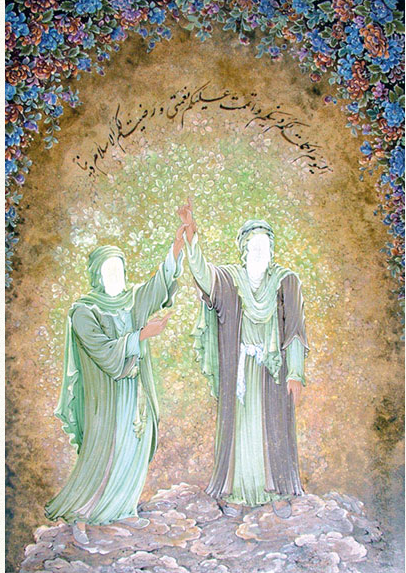
\includegraphics[width=1.35188in,height=1.90972in]{Images/image078.png}
    \caption{Ġadir-e Khumm et la
désignation de l'Imâm `Alī. œuvre de Rezâ
Badr-os-Samâ'}
    \label{Ġadir-e Khumm}
\end{marginfigure}

Il y reçut le verset suivant~: 
\begin{quote}
  {«~O Messager, transmets
ce qui t'a été descendu de la part de ton Seigneur. Si tu ne le faisais
pas, alors tu n'aurais pas communiqué Son message. Et Dieu te protégera
des gens. Certes, Dieu ne guide pas les gens mécréants.~» (Coran,
5:67).}  
\end{quote}


Par la suite, selon les šī`ites, Muḥammad déclara~: «~Man kuntu Mawlāhu,
fahaza `Alī mawlāhu~» c'est-à-dire~: «~Qui me reconnaît comme son Mawlā
(maître, guide), doit reconnaître `Ali comme son Mawlā ~».




Mais pour certains des compagnons du Prophète, cette désignation n'a
jamais été officialisée et selon les mœurs tribales, il convient donc de
procéder à son élection.

Mais `Alī est écarté du collège électoral. \mn{\cite{OUARDI:CalifesMaudits}} 

La tribu des Qurayš élit Abū Bakr, vieux compagnon et un des beaux-pères
de Muhammad~: il devint le 1\textsuperscript{er} calife (khalîfa).

`Alī fera acte d'allégeance, il se soumet à ce choix signifiant son
désir de maintenir l'unité de l'\emph{umma}.

À la mort d'Abū Bakr, `Umar devient le 2\textsuperscript{ème} calife
puisqu'il avait été désigné de manière explicite (\emph{naṣṣ}). `Alī
accepte.

`Umar annonce qu'à sa mort, son successeur devra être choisi parmi les
membres d'un collège électoral qu'il a lui-même nommés. `Alī en fait
partie. À la mort de `Umar, c'est `Uṯmān qui est choisi. Accusé de
népotisme, il est assassiné.

`Alī devient alors le 4\textsuperscript{ème} calife (656-661) attestant
ainsi de ses qualités vertueuses et de la suprématie de l'imamat sur les
manigances politiques mondaines.

Pour autant, deux anciens compagnons du Prophète n'ayant pas vu leur
appétit politique satisfait -- ils souhaitaient être gouverneurs de Kūfa
et Baṣra -- s'associèrent à `Ā'iša, fille d'Abū Bakr et veuve du
Prophète, pour lever une armée contre `Alī. C'est la bataille du chameau
de 657. On l'appelle ainsi parce que `Ā'iša qui était présente, était
montée sur un chameau\ldots{} Son armée fut mise en défaite.





\mn{On voit ici `Ā'iša sur son chameau et dans son baldaquin}



Mais en Syrie, Mu`āwiya, parent de `Uṯmān, mena aussi une guerre. C'est
la bataille de Ṣiffīn. Alors qu'elle tournait à l'avantage de `Alī,
Mu`āwiya proposa un arbitrage sur le livre sacré. `Alī accepte. Nombre
de ses soldats se soulèvent considérant qu'il n'avait pas à accepter
l'arbitrage et que Dieu avait déjà rendu son jugement par la victoire
qui se manifestait. `Alī doit mener combat contre ces rebelles (ce sont
les ḫariǧites), alors que Mu`āwiya se fait proclamer calife à Jérusalem
en 660~!

`Alī est assassiné par un ḫarigite à Kūfa en 661.

Pour les sunnites, il n'avait pas de successeur tandis que les šī`ites
affirment qu'il avait nommé son fils aîné, al-Ḥasān.

 
\subsection{La généalogie du
šī`isme}\label{la-guxe9nuxe9alogie-du-ux161ux12bisme}

La généalogie est sujet à controverses et divergences ce qui explique la
multiplication des šī`ismes\textbf{.} On dénombre une centaine de
lignées à la fin du premier siècle de l'Hégire.

Les jours de naissances des membres de la famille de `Alī sont des fêtes
religieuses. Les jours anniversaires de leur mort, des journées de
deuil. Leurs tombes sont des lieux de pèlerinage~: les cités où elles se
trouvent sont des villes saintes.

Elle est un peu subtile, chaque imām mériterait un chapitre\ldots{}
entre son enseignement, les histoires, les légendes, leur assassinat --
souvent empoisonné -- sans compter qu'au sein même du šī`isme, les
généalogies, les filiations ne sont pas les mêmes, que certains ne
reconnaissent que quatre imāms, d'autres sept, d'autres douze, que ce ne
sont pas toujours les mêmes\ldots{} qu'il y a donc une multitude de
branches šī`ites\ldots{} Bref, je retiens surtout le šī`isme majoritaire
dit duodécimain, car il reconnaît 12 imāms. Vous en trouverez en annexe
la liste avec leurs noms et quelques caractéristiques. Si vous avez la
curiosité de regarder le douzième, vous voyez que n'est pas indiquée la
date de sa mort. D'après vous, est-ce parce que l'on ne la connaît pas,
ou est-ce pour une autre raison~? La réponse dans la suite du cours. Bon
travail.

 
\paragraph{`Alī et Fātima}\label{alux12b-et-fux101tima}

`Alī joue donc dans le šī`isme un rôle important. Il est à la tête de
presque toutes les chaînes de transmission, il est considéré ~comme un
maître spirituel. On lui attribue deux livres~: \emph{Nahj al-balâgha}
(La Voie de la maturité)~et \emph{Dîwân}, un recueil de poèmes.

Quant à Fātima, elle est la sainte la plus vénérée du šī`isme\textbf{.}
Sa tombe est à Médine (il y en a trois\ldots{} dans le doute, on les
garde toutes les trois).

Fātima est la mère de toute la lignée des imāms. Elle représente ce qui
relie Muhammad à `Ali, la lettre et l'esprit. Elle est dite \emph{maǧma`
al-nūrayn} (le Confluent des Deux Lumières), celle de la prophétie et de
l'imamat. Elle a une mission d'intercession et de protection jusqu'à la
fin des temps. Immaculée, Vierge malgré son mariage, elle est aussi
reine du ciel. Un parallèle avec Mariam (Marie), la mère de Jésus est
établi par la tradition šī`ite elle-même \sn{Tahani Sabri,
  «~L'hagiographie de Fāṭima d'après le \emph{biḥār al-anwār}~», École
  des Hautes Études en Sciences Sociales, thèse de doctorat sous la
  direction de Henry Corbin, 1969.}.

 
\paragraph{Al-Hasan, fils de
`Alî}\label{al-hasan-fils-de-aluxee}

C'est un petit-fils du Prophète. Il y a des récits touchant d'affection
tendre.

Al-Ḥasan abdiqua le califat devant l'hostilité de Mu`āwiya. Pour les
historiens šī`ites, il préféra l'unité de la communauté plutôt que de
voir la division, mais les sunnites font remarquer qu'il n'était pas en
mesure de remporter la victoire et qu'il abdiqua en contre-partie d'une
importante somme d'argent. Retiré à Médine, il est assassiné,
semble-t-il par une de ses épouses qui aurait été soudoyée, selon les
šī`ites par Mu`āwiya. Terrible Mu`āwiya\ldots{} J'imagine que vous ne
devez pas le trouver très sympathique. Il est le fondateur de la
dynastie Omeyyade. Les grands historiens sunnites des
8\textsuperscript{ème} et 9\textsuperscript{ème} siècles n'en ont pas
laissé un souvenir très élogieux\ldots{} car ils sont abbassides et il
fallait effacer les traces vénérables des Omeyyades.

 
\paragraph{Al-Ḥusayn} 

Al-Ḥusayn, le second fils de `Alī, reste discret. Il s'efface. Mais il
entre sur la scène politique au moment de la mise en place d'une
dynastie califale héréditaire en la personne de Yazīd, le fils de
Mu`āwiya. On se réfère souvent à lui pour présenter le šī`isme comme un
courant révolutionnaire, politique et contestataire.

L'histoire est plus complexe. En tous les cas, les sources appellent une
très grande prudence. Assuré du soutien de la ville de Kūfa, il se met
en route avec toute sa famille pour chasser les Omeyyades. Mais sur la
route, la petite troupe se trouve encerclée par les soldats omeyyades,
coupée de Kūfa, privée d'eau. Retranchée en plein désert dans un petit
village appelé Karbalā', les Omeyyades finissent par donner l'assaut.
C'est un massacre. Ḥusayn est tué, décapité, piétiné ainsi que quasiment
toute sa famille.

Ašura est le jour de célébration où l'on fait mémoire de cette tragédie
dans de grandes cérémonies populaires avec parfois des dérives
spectaculaires de lamentations violentes, d'auto-flagellations, de
lacérations ou de mutilations. C'est le remord d'une ville qui n'a pas
soutenu al-Ḥusayn.

Ḥusayn devint alors un exemple de martyr, de sacrifice, de bravoure.
Sans-doute, sous l'influence chrétienne, on verra dans la mort de Husayn
un sacrifice rédempteur pour le salut des fidèles.

Chez certains fidèles la rumeur selon laquelle il ne serait pas mort
circule. Il aura été enlevé au ciel directement par Dieu avant le
combat.


\mn{Les troupes omeyyades encerclent Karbalā' \& Yā Ḥusayn\ldots{}

Jour de la fête d'Ashura \& Ashura et ses spectaculaires flagellations à
Karbalā'\ldots{} }


 
\paragraph{`Alî Zayn al-`Âbidîn, fils
d'al-Husayn}\label{aluxee-zayn-al-uxe2biduxeen-fils-dal-husayn}

Un rescapé du massacre de Karbalâ'. Il serait parti à Médine pour y
mener une vie pieuse. Il ne posa aucun problème aux Omeyyades. Une
existence ascétique, consacrée à la dévotion. On le surnommait
\emph{al-saǧǧād}, celui qui accomplit de nombreuses prosternations.
C'est un nom respecté, même dans le sunnisme.

Un de ses fils Zayd ibn `Alî, est à l'origine d'une grande famille, les
zaydites. Le zaydisme est marqué par un activisme violent. Selon la
théorie zaydite de l'imamat chaque Alide a le droit de prétendre à la
direction de la communauté. Le véritable imâm est celui qui se qualifie,
les armes à la main, en s'insurgeant contre le pouvoir injuste. Ils sont
aujourd'hui encore influents au Yémen~où ils représentent la moitié de
la population (mais le dernier chef zaydite du Yémen a été renversé en
1962).

 
\paragraph{Muhammad al-Bāqir, fils de `Alî Zayn
al-`Âbidîn}\label{muhammad-al-bux101qir-fils-de-aluxee-zayn-al-uxe2biduxeen}

Il est considéré comme le fils de `Ali Zayn. Les grandes traditions
šī`ites le considèrent comme le 5ème Imām. Il est surnommé Abū Ǧa`far.

 
\paragraph{Ǧa'far al- Ṣādiq
}\label{ux1e7afar-al--ux1e63ux101diq}

Fils de Muhammad al-Bāqir, il est célèbre pour sa piété et, selon les
shiites, l'infaillibilité de ses prémonitions. Les auteurs soufis lui
attribuent le plus ancien commentaire mystique du Coran. On le considère
comme un alchimiste, un spirituel refusant toute implication dans les
mouvements politiques de son époque. Il fut enterré dans le cimetière de
Baqī` à Médine. Le carré šī`ite y sera rasé au XIX° siècle par les
Wahhabites, alors qu'il abritait les tombes de plusieurs imâms.

Son fils aîné, Ismā`īl, est l'éponyme de la seconde grande famille de
l'islam šī`ite, les ismaéliens, šī`ites septimains \textbf{--} shî'ites
à 7 imâms. Pour cette branche, il est le dernier Imâm. Un autre groupe
s'appuie sur la croyance que l'imamāt fut transmis du vivant de Ǧa`far à
son petit-fils~: ce sont les qarmates. D'autres, les Fatimides,
considèrent que l'imamat se poursuit et que l'imam caché, le Mahdi, sera
un de ses descendants.


\begin{Synthesis}
Le si'isme est  une prophétologie. Il y a une sur
l'incarnation. Facilite le
dialogue avec les chrétiens.
\end{Synthesis}

 
\paragraph{{Le douzième imām, l'imām caché ou
le Madhī
}{ }}\label{le-douziuxe8me-imux101m-limux101m-cachuxe9-ou-le-madhux12b}

À la mort du 11\textsuperscript{ème} imâm, les fidèles croient que
l'imâm a eu un fils du nom de Muḥammad. 
\begin{Def}[Mahdî]
Il est reconnu comme le
\emph{Mahdî,} le Bien Guidé. C'est l'imâm caché, \emph{al-imâm al-ġā'ib}
ou encore \emph{al-Qā'im}, que l'on peut traduire par le Résurrecteur.
\end{Def}


C'est le courant duodécimain, majoritaire dans le šī`isme.

Mais en quoi consiste cette occultation~? Comment s'opère-t-elle~? Que
signifie-t-elle~? Quand a-t-elle eu lieu~? Sous quelles formes~?

Je vous propose d'écouter ce bref passage d'une émission sur France
Culture, «~Les racines du ciel~», où Amir-Moezzi répond.

L'imâm caché n'est donc pas mort. Vous comprenez maintenant pourquoi
dans le tableau en annexe ne figure que sa date de naissance. Il
n'existe pas de successeur puisqu'il est physiquement vivant. À la fin
des temps, il se manifestera. Il y a donc une présence invisible, mais
physiquement réelle. L'imâm caché clôt la lignée des imamites.

Par la suite, tout se passe comme si désormais l'ère de la bonne entente
entre le religieux et le politique était désormais finie. La cité
idéale, gouvernée par un juste n'est réalisable qu'à la fin des temps,
avec l'avènement du Mādhi, le Sauveur eschatologique. L'attitude
revendicative et politique est rejetée dans un futur messianique. Le
šī`isme se présente comme une religion individuelle, personnelle, non
institutionnelle. Mais peut-il alors perdurer ? Pour pallier cette
«~absence~», on aura recours à la figure du juriste avec la dynastie
bouyide. C'est à cette époque que le šī`isme sera érigé comme religion
d'État, ce qui n'est pas le moindre des paradoxes compte tenu de ses
«~fondamentaux~».

 
\section{Les fondations du šī`isme~:
doctrines}\label{ii.-les-fondations-du-ux161ux12bisme-doctrines}

Les doctrines šī`ites sont compliquées, subtiles et à lire
l'enseignement des imāms et les commentaires qui en suivirent, cette
subtilité est voulue pour elle-même. De leurs enseignements, ils ne
cessent de dire~: «~notre enseignement est ardu, difficile à supporter~:
c'est un secret, un secret enveloppé par un secret au sujet d'un
secret~»\sn{Voir Amir-Moezzi, Jambet, \emph{Qu'est-ce que le
  shi'isme~?}, Paris, Fayard, p. 96 .}.

Dans sa présentation du šī`isme, Amir-Moezzi distingue dans la vision du
monde et la théologie šī`ite une double dimension~: elles sont marquées
à la fois par l'affirmation d'un principe de dualité et d'un principe de
dualisme. On lira avec intérêt et pour plus de précisions la
présentation qu'il fait dans \emph{Qu'est-ce que le shiisme~?} Mais tout
d'abord, la question des Écritures. Sont-elles les mêmes qu'en
sunnisme~?

 
\subsection{{Les sources scripturaires
}}\label{les-sources-scripturaires}

 
\paragraph{{Y a-t-il un Coran šī`ite~?
}}\label{y-a-t-il-un-coran-ux161ux12bite}

Le Coran est la référence principale et la contradiction éventuelle
entre un \emph{ḥadīṯ} et un verset coranique est l'indice de la fausseté
du ḥadīṯ.

Pour autant, certaines traditions shî'ites trouvent difficilement leur
fondement dans le Coran. Pour les šī`ites, le Coran a été en réalité
falsifié, altéré, censuré lors de sa compilation par `Uṯmān (c'est un
des premiers califes. Si le nom ne vous disait plus rien du tout,
revoyez le premier cours sur le Coran et à la question du
\emph{muṣhaf}). La révélation originelle contenait des versets sur `Alî
et les descendants des Prophètes. Ils étaient cités comme les modèles et
les chefs par excellence. `Alī possédait une version du Coran intégral,
mais il n'en dit mot pour éviter sa destruction par ses adversaires.
Cependant, elle fut transmise secrètement d'imam à imam, jusqu'au
12\textsuperscript{ème} imâm qu'il l'emporta avec lui lors de son
Occultation. Les enseignements des imāms permettent d'accéder à ces
versets et de les connaître.

Avec l'arrivée au pouvoir des Bouyides shiites à la fin du
4\textsuperscript{ème} siècle de l'hégire, il s'agira de trouver un
accord avec l'orthodoxie sunnite. On met ainsi un terme au doute sur
l'intégrité du Coran officiel. Le courant dominant abandonne la thèse de
la falsification du Coran officiel, mais le débat ressurgit
régulièrement.

 
\paragraph{Y a-t-il un \emph{ḥadīṯ} šī`ite~?
} 

Bien qu'al-Būḫārī fut perse, il existe une Sunna šī`ite. Les textes sont
bien souvent les mêmes, mais les \emph{isnāds} diffèrent et renvoient
aux membres de la famille du prophète (\emph{ahl al-bayt} --
c'est-à-dire littéralement, les gens de la maison). En effet, la
référence dans l'\emph{isnād} aux compagnons du Prophète lui ôte toute
crédibilité dans la mesure où ils sont considérés comme des traîtres.
Pour l'\emph{isnād}, la notion a été vue dans le cours sur la Sunna.
C'est la fameuse chaîne de transmission.

On reconnaît trois grands corpus~:

\begin{itemize}
\item
  Celui de Ya`qub al-Kulaynī (m. en 939).
\item
  Celui de Saduq Ibn Babuyeh (m. 991).
\item
  Celui d'al-Ḥasan al-Tusī (m. 1068).
\end{itemize}

On trouve aussi dans ces recueils de nombreux témoignages des imāms.

L'ouvrage le plus connu de Kulaynī est \emph{al-Kāfī}. Il est divisé en
trois sections~:

\begin{itemize}
\item
  \emph{Usūl al-Kāfī}, qui concerne l'épistémologie, la théologie, la
  question de la foi et de la mécréance, l'histoire, l'éthique, et le
  Coran~et ses mérites;
\item
  \emph{Furūʿ al-Kāfī}, qui concerne les dimensions pratiques et légales
  (prières, \emph{ǧihād}, jeûne, ḥaǧǧ, funérailles, nourriture, boisson,
  mariage, divorce, commerce, héritage, etc.)
\item
  \emph{Rawdat} \emph{al-Kāfī}, qui inclue de nombreuses traditions, des
  lettres, des discours des imāms.
\end{itemize}

Il existe une traduction anglaise de cette collection de plus de 16 000
traditions. Si vous ne trouvez pas le sommeil\ldots{}
 
\subsection{ Dualité et dualisme}\label{dualituxe9-et-dualisme}

 
\paragraph{ Une vision duelle}\label{une-vision-duelle}

Il s'agit d'affirmer que toute réalité possède deux niveaux~:

1/ un niveau manifeste, obvie, apparent, visible, concret, évident
(\emph{zāhir})

2/ un niveau secret, non manifeste, implicite, invisible, intérieur
(\emph{bāṭin})

Cette affirmation est au cœur du credo šī`ite. Ce que je vois, ce qui
est visible contient aussi une réalité invisible. Il existe une relation
entre le manifeste et le caché, l'exotérique et l'ésotérique. Il s'agit
d'appliquer ce principe à toute réalité, et bien sûr, à commencer par la
théologie.

\emph{Ainsi, en théologie}, Dieu a deux niveaux d'être, deux niveaux
ontologiques~:

1/ son Essence, inconcevable, inimaginable, au-delà de toute pensée~:
c'est le niveau caché (\emph{bāṭin})

2/ ses Noms et Attributs~à travers lesquels Dieu se révèle et se fait
connaître~: c'est le Dieu inconnu qui aspire à être connu. Amir-Moezzi
remarque que l'on retrouve une distinction de la théologie médiévale
chrétienne entre \emph{Deus absconditus} et \emph{Deus revelatus}.

La manifestation de ces noms divins comme le Roi, le Miséricordieux, le
Juge suprême, etc. est une manifestation de Dieu (théophanie). La plus
haute révélation en est la figure de l\emph{'Imām} céleste,
l'\emph{Imām} de Lumière, l'Homme cosmique~: c'est l'Imām avec un I
majuscule, dans son acception ontologique universelle.

L'\emph{Imām} cosmique a aussi deux dimensions

\begin{quote}
1/ la dimension cachée~: c'est l'aspect métaphysique, dans le ciel,
invisible à nos yeux.

2/ la dimension exotérique, visible~: ce sont les \emph{imāms}
historiques.
\end{quote}

La mission de ces \emph{imāms} historiques~consiste à dévoiler les
mystères de Dieu, du monde et de l'homme, à transmettre aux hommes le
Secret contenu dans l'Imām métaphysique.

Mais l'enseignement des imāms, disions-nous, est complexe. Ǧa`far
al-Ṣādiq (c'est un \emph{imām} que nous avons rencontré dans la
généaologie des douze\ldots{} C'est le combientième \emph{imām} déjà~?)
écrivait~: «~Notre enseignement comporte l'exotérique, l'ésotérique et
l'ésotérique de l'ésotérique~».

À cette approche duelle de la réalité se superpose le principe du
dualisme.

 
\paragraph{ Une vision dualiste}\label{une-vision-dualiste}
\mn{Si isme~: influence de la zoroastrisme avec un certain manichéisme, bien
/ mal. Lumière et nuit~; combat cosmique et sur terre. On retrouve ceci
dans le sunnisme. Tous les Hadiths eschatologiques décrivent en tableau
le paradis. Dans le Si isme, enjeu du bien et du mal.
}
L'histoire de la création est celle d'un combat cosmique entre les
forces du Bien et les forces du Mal, entre la lumière et l'obscurité. On
retrouve ici une nette dimension zoroastrienne et manichéenne du monde.

Ce combat se situe au niveau cosmique~: c'est le combat entre les armées
de l'Intelligence cosmique (\emph{al-`aql}) et celles de l'Ignorance
cosmique (\emph{al-ğahl}). Cette dichotomie, cette opposition est celle
d'une lutte permanente entre les Gens de la Droite (\emph{ašāb
al-yamīn}) et les gens de la Gauche (\emph{ašāb al-šimāl}). Le combat
entre deux hommes ennemis s'inscrit donc dans un cadre plus large. Toute
l'histoire de l'humanité est traversée par l'adversité et la violence
des forces démoniaques de l'Ignorance. Il en sera ainsi jusqu'à la fin
des temps avec l'avènement du Sauveur eschatologique, le Mahdī qui
vaincra définitivement les forces du mal.

Mais qui sont ces forces du mal~? Comment les reconnaître, les
identifier~?

C'est l'enseignement des imāms (les 7, les 12, selon) qui apportent les
réponses à ces questions. Dans ce corpus de centaines de milliers de
pages, les adversaires de l'imâm~sont tour à tour identifiés~:

\begin{itemize}
\item
  Aux juifs, qui sont des idolâtres et ont trahi Moïse en adorant le
  veau d'or
\item
  Aux Compagnons de Muhammad qui ont rejeté `Alī
\item
  Aux Gens de l'exotérique, c'est-à-dire des apparences, du superficiel
  (\emph{ahl al-zāhir}), ce sont les littéralistes qui s'arrêtent à la
  lettre et n'ont pas connaissance de son `esprit' (\emph{bāṭin}). À cet
  égard, un šī`ite se sentira plus proche d'un juif ou d'un chrétien
  accoutumé à une lecture ésotérique, symbolique, anagogique des textes
  que d'un musulman sunnite exotérique, qui se limite à la lettre.
\end{itemize}

 
\subsection{Prophétie et
Imamologie}\label{prophuxe9tie-et-imamologie}

L'enseignement des \emph{imāms}, acquiert en réalité un rôle supérieur à
celui du Prophète.

En effet, si le prophète est le messager de la lettre, l'\emph{imām}
dans le šī`isme en apporte l'esprit. Or, si l'esprit peut exister sans
la lettre, sans l'esprit, la lettre est morte\sn{Amir-Moezzi,
  Jambet, \emph{Qu'est-ce que le shi'isme~?}, Paris, Fayard, 2004, p.
  42.}.


\paragraph{Remarque sur l'imām~}: le mot \emph{imām}
est piégé. Il s'emploie en sunnisme, mais sans désignation particulière.
L'imām désigne un savant, un chef ou tout simplement celui qui dirige la
prière. En revanche, en šī`isme\textbf{,} c'est un titre sacré. L'imām
est le Guide, l'un des Douze\ldots{} En principe, aucun autre homme ne
porte ce nom. Et pourtant, d'aucuns se sont attribués ce titre. Autant
dire qu'ils se prenaient pour le Mahdi .L'un d'eux est très célèbre. À
suivre.

L'Imām apporte en effet la connaissance face au monde de l'ignorance. En
montrant son cœur, l'Imām `Alī donnait cet enseignement sur la vocation
de l'imām, la nature de la religion, son importance. Écoutez et
réécoutez ce texte\sn{Vous trouvez l'intégralité du texte dans le
  livre de Mohammad Ali Amir-Moezzi, \emph{La religion discrète}, Paris,
  Vrin, 2006,
  \url{https://books.google.com}}.


L'imām transmet les vérités secrètes. Il tient le monde, il évite la
noyade définitive du monde dans les ténèbres. Il est l'alpha et l'omega
du šī`isme\sn{Amir-Moeezi, Jambet, \emph{Qu'est-ce que le
  shi'isme~?}, p. 40.}.

Mais il a aussi des pouvoirs supra-normaux~: il possède la science du
passé et du futur, il lit dans les consciences, il connaît les langues,
y compris celle des animaux, les sciences occultes (astrologie,
alchimie, sciences divinatoires, etc.). Il peut ressusciter les morts,
guérir les maladies, rajeunir les vieillards, marcher sur les eaux,
monter aux cieux\ldots{} Il possède des objets de pouvoir~ tels la
tunique d'Adam, le sceau de Salomon, l'Arche et les tables de la Loi,
l'Arme invincible de Muḥammad.

L'enseignement de l'\emph{imām} est au cœur de l'approche spirituelle
šī`ite. C'est par lui que se réalise la spiritualisation, la
divinisation. Écoutez Amir-Moezzi à ce sujet.

 
\subsection{La walāya au cœur de la foi šī`ite
} 


La \emph{walāya} est un concept clé du \emph{šī`isme}. Les
\emph{šī`ites} sont appelés les gens de la \emph{walāya}.\\
\begin{Def}[walāya]
La \emph{walāya} désigne la mission sacrée et sainte des imams.

L'imām est le \emph{walī} (le saint), celui qui initie les fidèles à
l'esprit de la Parole divine. Il est la Face de Dieu sur terre.

\end{Def}



La \emph{walāya} désigne aussi l'amour, celui que les fidèles
manifestent dans la dévotion, par la loyauté, la soumission à l'égard du
maître initiateur.

Mais dans une doctrine \textbf{dualiste}, l'amour de l'imām ne peut aller sans la
haine de son ennemi. La \emph{walāya} est donc inséparable de son
contraire, la \emph{barā'a} (c'est-à-dire la haine, la dissociation à
l'égard des forces de l'ignorance). Un \emph{ḥadīṯ} šī`ite dit~:

\begin{quote}
«~l'amour de Dieu ne s'obtient que grâce à l'amour envers Ses amis et
l'hostilité à l'égard de Ses ennemis~».    
\end{quote}


Au cœur de la foi šī`ite, la \emph{walâya} est dans la \emph{šahāda} :
\begin{quote}
   «~Je témoigne qu'il n'y a pas de dieu hormis Dieu~; je témoigne que
Muhammad est l'envoyé de Dieu, et que `Alî est le \emph{walī} de
Dieu~» 
\end{quote}
 \emph{walī} signifie ici l'ami,~l'allié, le détenteur de la
\emph{walāya}.




\mn{\emph{Šahāda} sur une mosquée du Caire
fatimide. on y lit à la fin~:\emph{ʿAlī walī
allāh.
}  }


\subsection{{Les signes de la fin du monde ou
l'eschatologie šī`ite
}\label{les-signes-de-la-fin-du-monde-ou-leschatologie-ux161ux12bite}}

En raison de la place de la question de l'Occultation, l'eschatologie a
donné lieu à un foisonnement de traditions et de traités. Il s'agit de
savoir lire les signes afin de reconnaître l'imminence du Dernier Jour,
le retour du Mahdī. Les signes sont multiples, mais on peut identifier
quelques constantes~:

\begin{itemize}
\item
  l'envahissement de la terre par les forces du Mal,
\item
  l'écrasement quasi-complet des forces de la Connaissance par celles de
  l'ignorance,
\item
  la perte du sens du sacré,
\item
  le renversement des valeurs humaines,
\item
  l'anéantissement de tout ce qui relie l'homme à Dieu et à son prochain
\end{itemize}

Des signes concrets sont exposés. Ainsi par exemple,

\begin{itemize}
\item
  la venue d'al-Sufyānī, le chef de l'armée des ennemis des imāms, le
  collaborateur d'\emph{al-Daǧǧāl}, l'Imposteur, l'Antéchrist islamique.
\item
  L'avènement d'al-Yamānī, le Yéménite qui prêchera le soutien au Mahdī.
\item
  Le Cri, d'origine surnaturelle, venu du ciel, appelant les hommes à
  rejoindre l'armée du Sauveur
\item
  L'engloutissement d'une armée (parfois celle d'al-Sufyānī) dans le
  désert.
\item
  L'assassinat à La Mecque de l'envoyé du Mahdī, appelé \emph{al-Nafs
  al-Zakiyya\textbf{~}}: l'Âme Pure.
\end{itemize}

La fin de l'occultation est aussi expliquée et commentée. On peut en
distinguer 3 raisons~principales :
\begin{enumerate}
    \item une raison historique~: venger tous les hommes saints du passé,
victimes de l'injustice. Tous les saints du passé reviendront à la vie,
ainsi que leurs meurtriers, et les premiers pourront ainsi se venger des
seconds à cette occasion.
\item une raison religieuse~: rétablir le sens du sacré~; rétablir les
religions (judaïsme, christianisme, islam) dans leur intégralité
originelle, rapporter les Écritures respectives qui ont été altérées ou
falsifiées
\item une raison spirituelle~: apporter le sens ésotérique des choses,
effacer la frontière entre le caché et le manifeste.
\end{enumerate}
 

Le retour du Mahdi s'accompagne aussi de celui de Jésus-Christ. Il est
le principal compagnon d'al-Qā'im. Voyez un peu plus haut. C'est un nom
utilisé pour nommer le Mahdi. Quelle est sa signification déjà~? Penser
à «~\emph{Talitha Qum~}».. Lève-toi\ldots{} C'est bien la même racine du
redressement, de la résurrection.

 
\section{Bibliographie}\label{bibliographie}

\paragraph{Les fondamentaux}

Mohammad-Ali \textsc{Amir-Moezzi}, Christian Jambet, \emph{Qu'est-ce que
le shî'isme~?,} Paris, Fayard, 2004.

Henri \textsc{Corbin}, \emph{En Islam iranien}, Aspects spirituels et
philosophiques III, Les Fidèles d'amour, shî'isme et soufisme,
Gallimard, 1978, 359 pages (PISAI H266).

\paragraph{Pour aller plus loin}

Mohammad Ali \textsc{Amir-Moezzi}, \emph{La religion discrète},
Croyances et pratiques spirituelles dans l'islam shî`ite, Collection
Textes et Traditions dirigée par Marie-Odile Goulet-Cazé, Richard
Goulet, Philippe Hoffmann, Paris, Vrin, 2006.

Henri \textsc{Corbin}, «~De l'histoire des religions comme problème
théologique~», \emph{Monde non chrétien} 51-52, 1960

Leili \textsc{Echghi}, \emph{Un temps entre les temps~: L'Imam, le
Chî'isme et l'Iran}, coll. Patrimoines Islam, cerf, Paris, 1992.

Geneviève Gobillot, \emph{Les Chiites}, Editions Brepols, 1998.

Henri Laoust, \emph{Comment définir le sunnisme et le chiisme},
Geuthner, 1985, 44 pages.

Muhammad Ridā Muzaffar, \emph{Le credo des imamites}, traduction par
Frère Sliwa, Rome, PISAI.

Yann \textsc{Richard}, \emph{Le Šī`isme en Iran~: Imam et Révolution,
Librairie d'Amérique et d'Orient}, 1980, 142 pages.

Yann \textsc{Richard}, \emph{L'islam chi'ite~: croyances et idéologies},
Fayard, Paris, 1991.

\textbf{\hfill\break
}

\subsection{Généalogie des Imāms}


 

\begin{longtable}{p{0.5cm}p{1.3cm}p{1.8cm}p{2.5cm}p{3.5cm}p{0.8cm}}
\small \\
%\sidecaption{Généalogie des Imāms} \label{tab:Genealogie} \\
\toprule
 & Nom & Titre & Epithète & connu pour & dates
\\
\midrule
\endhead
1 
& 
\vtop{{ `Alī}{ (\TArabe{علي})}} 
&
\vtop{{ Abū al-Ḥassan}{ (\TArabe{أبو الحسن})}}
&
\vtop{{ Amīr al-Mu'minīn}{ (\TArabe{أمیر المؤمنین}) -
Commandeur des croyants}} 
& Le premier Imam est la personne la plus
significative après Mahomet pour les chiites 
& 600 -- 661 \\



2 & \vtop{{ Ḥasan}{ (\TArabe{ألحسن})}} &
\vtop{{ Abū Muḥammad}{ (\TArabe{أبو محمد})}} &
\vtop{{ Al-Mujtabā}{ (\TArabe{ألمجتبی}) - le choisi}}
& Signe un traité de paix pour un Islam meilleur, très aimé par Mahomet
est avec son frère un des maîtres des jeunes du paradis & 625 -- 669 \\


3 & \vtop{{ Ḥusayn}{ (\TArabe{ألحسین})}} &
\vtop{{ Abū \textsuperscript{c}Abdillāh}{ (\TArabe{أبو
عبداللھ})}} & \vtop{{ Sayyid
ash-Šuhadā'}{ (\TArabe{سید الشھداء}) - Seigneur des martyrs}} &
Est mort lors de la bataille de Kerbala. & 626 -- 680 \\


4 & `Alī (\TArabe{علي}) & \vtop{{ Abū
Muḥammad}{ (\TArabe{أبو محمد})}} & \vtop{{ Zayn
al-\textsuperscript{c}Ābidīn}{ (\TArabe{زین العابدین}) - Joyau
des croyants}} & Piété, jeûne, pénitence pendant 20 ans à cause de la
bataille de Kerbala. & 658 -- 713 \\


5 & Muḥammad (\TArabe{محمد}) & \vtop{{ Abū
Ja\textsuperscript{c}far}{ (\TArabe{أبو جعفر})}} &
\vtop{{ Al-Bāqir}{ (\TArabe{ألباقر}) - Pourfendeur de
la Science}} & le moins oppressé des douze imams par le calife de son
temps. Il n'est pas reconnu par les Zaydī (qui prennent comme imam Zayd
Ibn `Alī. & 676 -- 743 \\


6 & \vtop{{ Ǧa'far}{ (\TArabe{جعفر})}} &
\vtop{{ Abū \textsuperscript{c}Abdillāh}{ (\TArabe{أبو
عبداللھ})}} & \vtop{{ Aṣ-Ṣādiq}{ (\TArabe{ألصادق}) -
Le véridique}} & Un penseur respecté à la fois par les Chiites et les
Sunnites & 703 -- 765 \\


7 & \vtop{{ Mūsā}{ (\TArabe{موسی})}} &
\vtop{{ Abū Ibrāhīm}{ (\TArabe{أبو إبراھیم})}} &
\vtop{{ Al-Kāẓim}{ (\TArabe{ألکاظم}) - Le triste}} & A
grandi en prison pour le rendre faible Il n'est pas reconnu par les
ismaéliens & 745 -- 799 \\


8 & \vtop{{ `Alī}{ (\TArabe{علي})}} &
\vtop{{ Abū al-Ḥassan}{ (\TArabe{أبو الحسن})}} &
\vtop{{ Ar-Riḍā}{ (\TArabe{ألرضا})}} & Le seul Imam à
être enterré en Iran & 765 -- 818 \\


9 & Muḥammad

(\TArabe{محمد}) & \vtop{{ Abū
Ja\textsuperscript{c}far}{ (\TArabe{أبو جعفر})}} &
\vtop{{ At-Taqī}{ (\TArabe{ألتقي})}} & Un grand
débatteur & 810 -- 835 \\


10 & \vtop{{ `Alī}{ (\TArabe{علي})}} &
\vtop{{ Abū al-Ḥassan}{ (\TArabe{أبو الحسن})}} &
\vtop{{ Al-Hādī (\TArabe{ألھادي}),}{ an-Naqī
(\TArabe{ألنقي})}} & & 827 -- 868 \\


11 & Ḥasan (\TArabe{ألحسن}) & \vtop{{ Abū
Muḥammad}{ (\TArabe{أبو محمد})}} &
\vtop{{ Al-\textsuperscript{c}Askarī}{ (\TArabe{ألعسکري})}}
& L'avant-dernier imam, qui a vécu presque toute sa vie assigné à
domicile et qui prêchait tout de même. & 846 -- 874 \\


12 & Muḥammad

(\TArabe{محمد}) & \vtop{{ Abū Qāsim}{ (\TArabe{أبو
قاسم})}} & \vtop{{ Al-Mahdī}{ (\TArabe{ألمھدي})}} &
Imam actuel, connu pour être le Sauveur. Il est l'occultation. & 868
-- \\
\bottomrule
\end{longtable}

\chapter{Le chiisme : histoire et doctrines}

\mn{21/3/22}
\section{bibliographie}
 

\begin{quote}
AMIR-MOEZZI, M-A. \emph{La religion discrète : croyances et pratiques
spirituelles dans l'Islam shi'ite}, Vrin, Paris, 2006.

AMIR-MOEZZI, M-A. et JAMBET, Christian \emph{Qu'est-ce que le shî'isme
?}, Fayard, Paris, 2004.

CORBIN, Henry \emph{En islam iranien: aspects spirituels et
philosophiques,} 4 volumes, Gallimard, Paris, 1991.

HALM, Heinz \emph{Le Chiisme}, Paris, PUF, 1995.

RICHARD, Yann \emph{L'islam chi'ite : croyances et idéologies}, Fayard,
Paris, 1991.

*TABATABA'I, Muhammad Huseyn \emph{Le chiisme en islam}, Beyrouth,
Al-Bouraq, 2009.
\end{quote}


\section{Le chiisme dans l'histoire
  musulmane. Quelques grands
  repères.}
  \label{le-chiisme-dans-lhistoire-musulmane.-quelques-grands-repuxe8res.}

On aurait pu traiter le développement du Chiisme et du sunnisme car ils ne se développent pas en vase clos. Mais il y a de tels différences,  en particulier, il n'y a pas de \textsc{foisonnement des visions dans le chiisme} du fait de l'importance des clercs
  

 \subsection{La naissance du chiisme : un problème de succession}
 ALi est le gendre et cousin du Prophète.
 
 Ali gagne à sa cause les nouveaux convertis (Egypte, Irak,...) et deviennent partisans d'Ali. Lorsque le Usman est assassiné en 656, Ali est élu comme 4ème calife. 
 \begin{Def}[ahl al-bayt]
\emph{famille du Prophète (Mahomet, Ali, Fatima, Hasan,
Hoseyn)}
 \end{Def}
 
 \paragraph{Mu'awiyya }Mais il est contesté par Mu'awiyya, qui lui reproche de ne pas chercher le meurtrier de Osman. En 657, bataille de Siffin, où les deux parties du monde arabe s'affrontent. Les Khalijites sont ceux qui reprochent à Ali d'avoir accepté l'arbitrage qui suit la bataille de Siffin.
 Ali est assassiné. Le califat est récupéré par Mu'awiyya.
 
 \paragraph{fondation de la dynastie des Omeyyades} par Mu'awyya. Hussayn, second fils de Ali s'oppose à Mu'awyya et est massacré dans la \textsc{plaine de Kerbala} avec sa famille et ses partisans. C'est le traumatisme fondateur. Le 10ème jour (Ashoura) du mois de Muharram, on rappelle ce martyr.
 
 \paragraph{une mosaique de courants shiites autour de la succession de l'imam et sur sa nature}
 Aujourd'hui, il y a trois courants : 
 \begin{itemize}
     \item ismaeliens :  7 imams
     \item zaydites : reconnaissent 5 imams
     \item imamites ou duodécimains : reconnaissent 12 imams.
 \end{itemize}
 
 Le Mahdi\sn{le Mahdi est aussi présent dans le sunnisme mais on ne sait pas qui c'est. Moins d'attente} n'est pas mort, il est occulté mais selon les courants, ce n'est pas le même. 
 
 \begin{Def}[mahdi]
   \emph{« le voilé » : l'homme mystérieux qui viendra annoncer et
provoquer la fin des temps (= dernier imam (occulté) pour les chiites).}
 \end{Def}
 
 \paragraph{Vision eschatologique forte dans le chiisme} Lutte du dernier imams contre le Dajjal, équivalent de \textit{l'antéchrist.}. Cela donne un potentiel révolutionnaire, avec certaines personnes se proclamant \textit{mahdi}, avec un potentiel mobilisateur très puissant, généralement révolutionnaire, voulant renversé le pouvoir établi, avec une forte dimension de justice sociale.
 
 
 
 %-------------------------------------------------
 \subsection{ « Le siècle chiite » : Bouyides et Fatimides (Xe-XIe s)}
 
 
 \paragraph{Diffusion du Chiisme à la mort de Hussayn} Dans les classes pauvres. En Irak par exemple, une grande révolte au IX ème siècle, se réclamant du chiime
 
 \paragraph{les bouyides} dans l'empire Abassides au X-XI, les Bouyides utilisent la faiblesse du calife pour s'imposer comme vizir, qui concentre la réalité du pouvoir : de 975, pendant environ un siècle.  
 
 \begin{figure}
     \centering
 
     \sidecaption{Source: \emph{Historical Atlas of Islam}, Malise Ruthven \& Azim Nanji,
Harvard University Press, 2004, p. 42.}
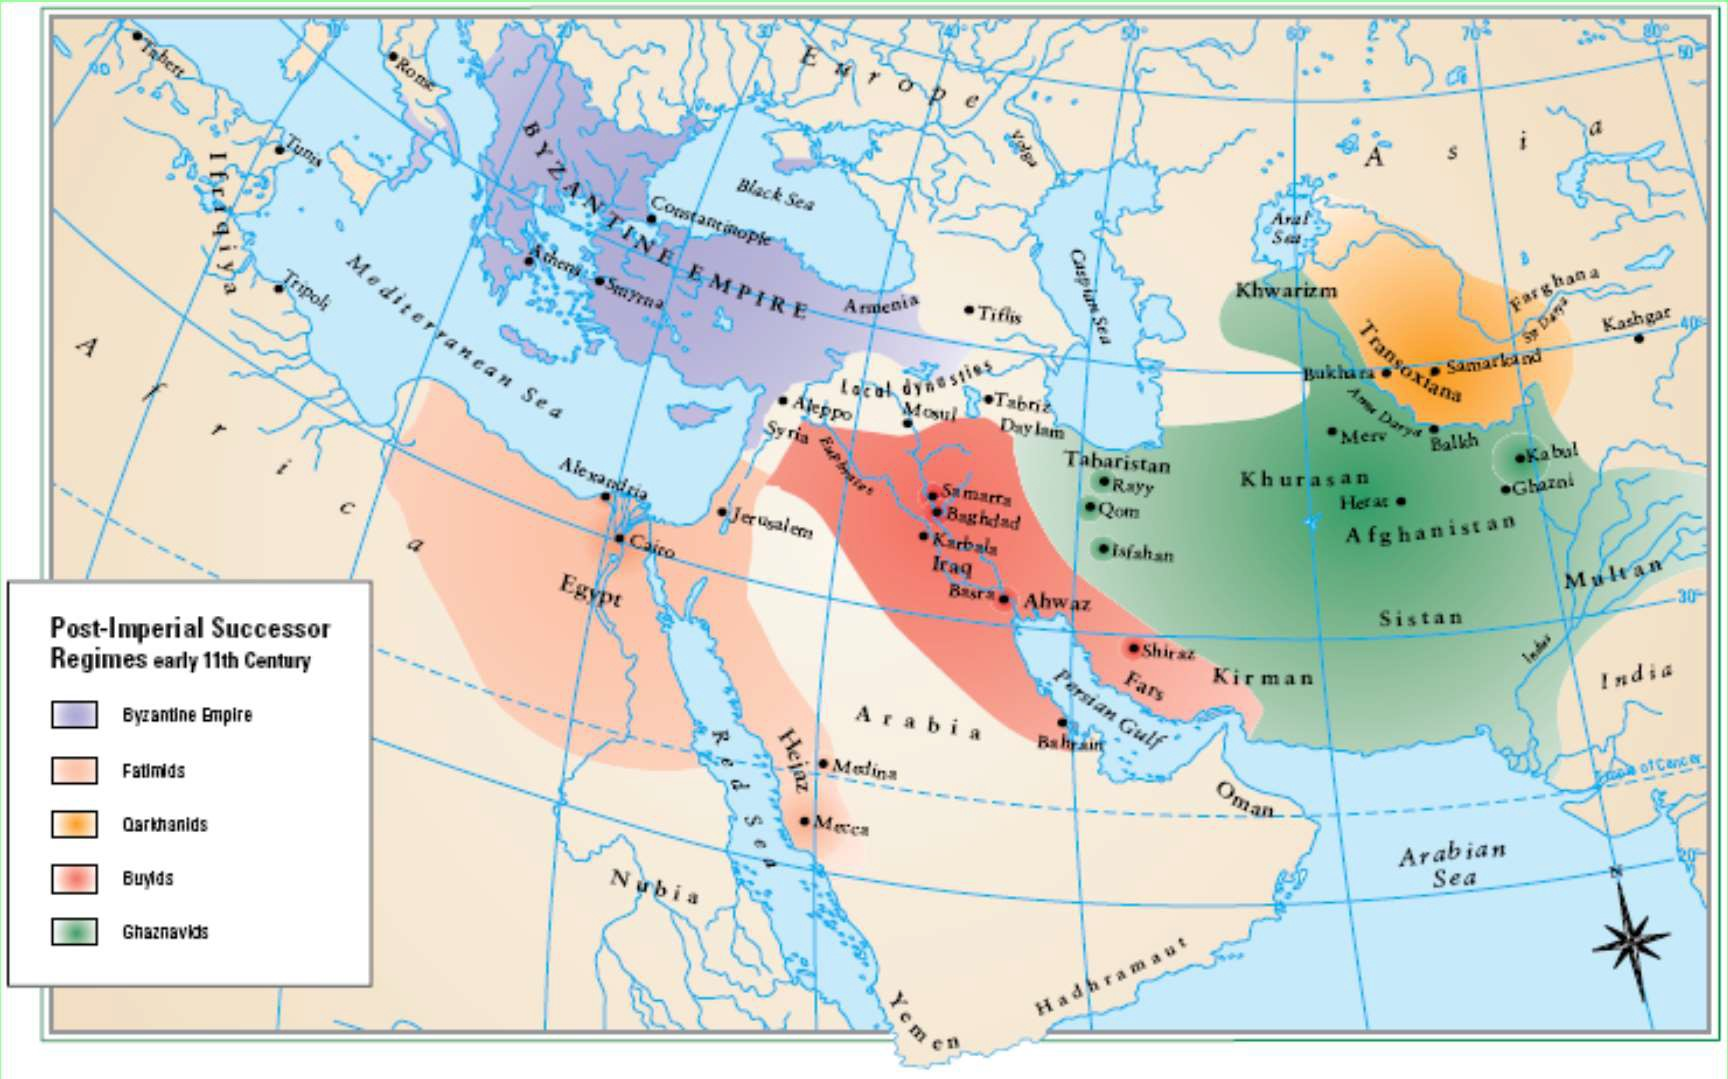
\includegraphics[width=\textwidth]{CourantsIslamContemporain/ImagesCourantsIslamContemporain/Image1Chiisme.jpeg}

     \label{fig:my_label}
 \end{figure}
 
 \paragraph{les fatimides} en afrique du Nord, fondé  par `Ubayd Allâh al-Mahdî (881-934). Typiquement, une personne se déclare Mahdi en Tunisie puis s'empare de l'Egypte (973 : le Caire comme capital). Avant le Caire n'était qu'une ville de garnison. 
 
 \paragraph{à Oman et au Yemen} AU Yémen, Zaydites, de 897 à 1962.
 
 
 %-------------------------------------------------
 
  \subsection{La naissance de l'Iran safavide (XVIe s.)}
 
  \begin{figure}
     \centering
 
     \sidecaption{Source: \emph{l'Iran safavide- Wikipedia}}
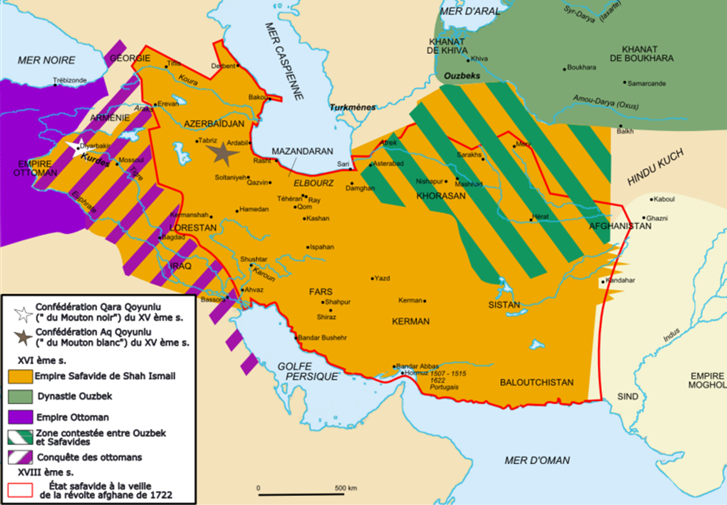
\includegraphics[width=\textwidth]{CourantsIslamContemporain/ImagesCourantsIslamContemporain/image2Chiisme.png}

     \label{fig:my_label}
 \end{figure}
 L'Iran était majoritairement sunnite jusqu'au Xème siècle. On a des populations turcophones à l'Ouest. un homme se proclame le Mahdi et fait la conquète militaire de l'Iran : par Isma'il en 1501.
  
 \paragraph{les limites du chiisme de Isma'il} conscient des limites du chiisme qu'il prone, il impose le chiisme duodécimain, venant du Liban, car le chiisme duodécimain était plus stable. Sans doute pour se détacher et légitimer face aux califes ottomans sunnites. Conversion de l'Iran assez violente : maudire les trois premiers califes, les confréries soufies. On va aussi déclarer les sunnites impurs.  


 
 %-------------------------------------------------
 
\section{Particularités de la doctrine chiite (duodécimaine ou imamite)
\label{particularituxe9s-de-la-doctrine-chiite-duoduxe9cimaine-ou-imamite}}


Elle s'est développée au VIII siècle par le 5ème et 6ème imams, qui étaient des savants. Ils ont collecté les corpus des hadiths, pas seulement du Prophète mais aussi des Imams, en particulier d'Ali et du 5ème et 6ème imams.

Ils ont développé l'école juridique
\begin{Def}[Ja'fariya]
 L'école juridique (madhhab) chiite dit Ja'fariya (aussi appelée école des Ahlul bayt) est la première école islamique apparue d'interprétation de fiqh du Coran d'inspiration chiite (contrairement aux quatre grandes écoles sunnites, avec lesquelles elle ne présente cependant pas de différences majeures).
\end{Def}
 %-------------------------------------------------
 
  \subsection{L'Imamat}
 La vraie spécificité du chiisme par rapport au sunnisme. 
 \begin{figure}[h!]
    \centering
        \sidecaption{lignée des imams}
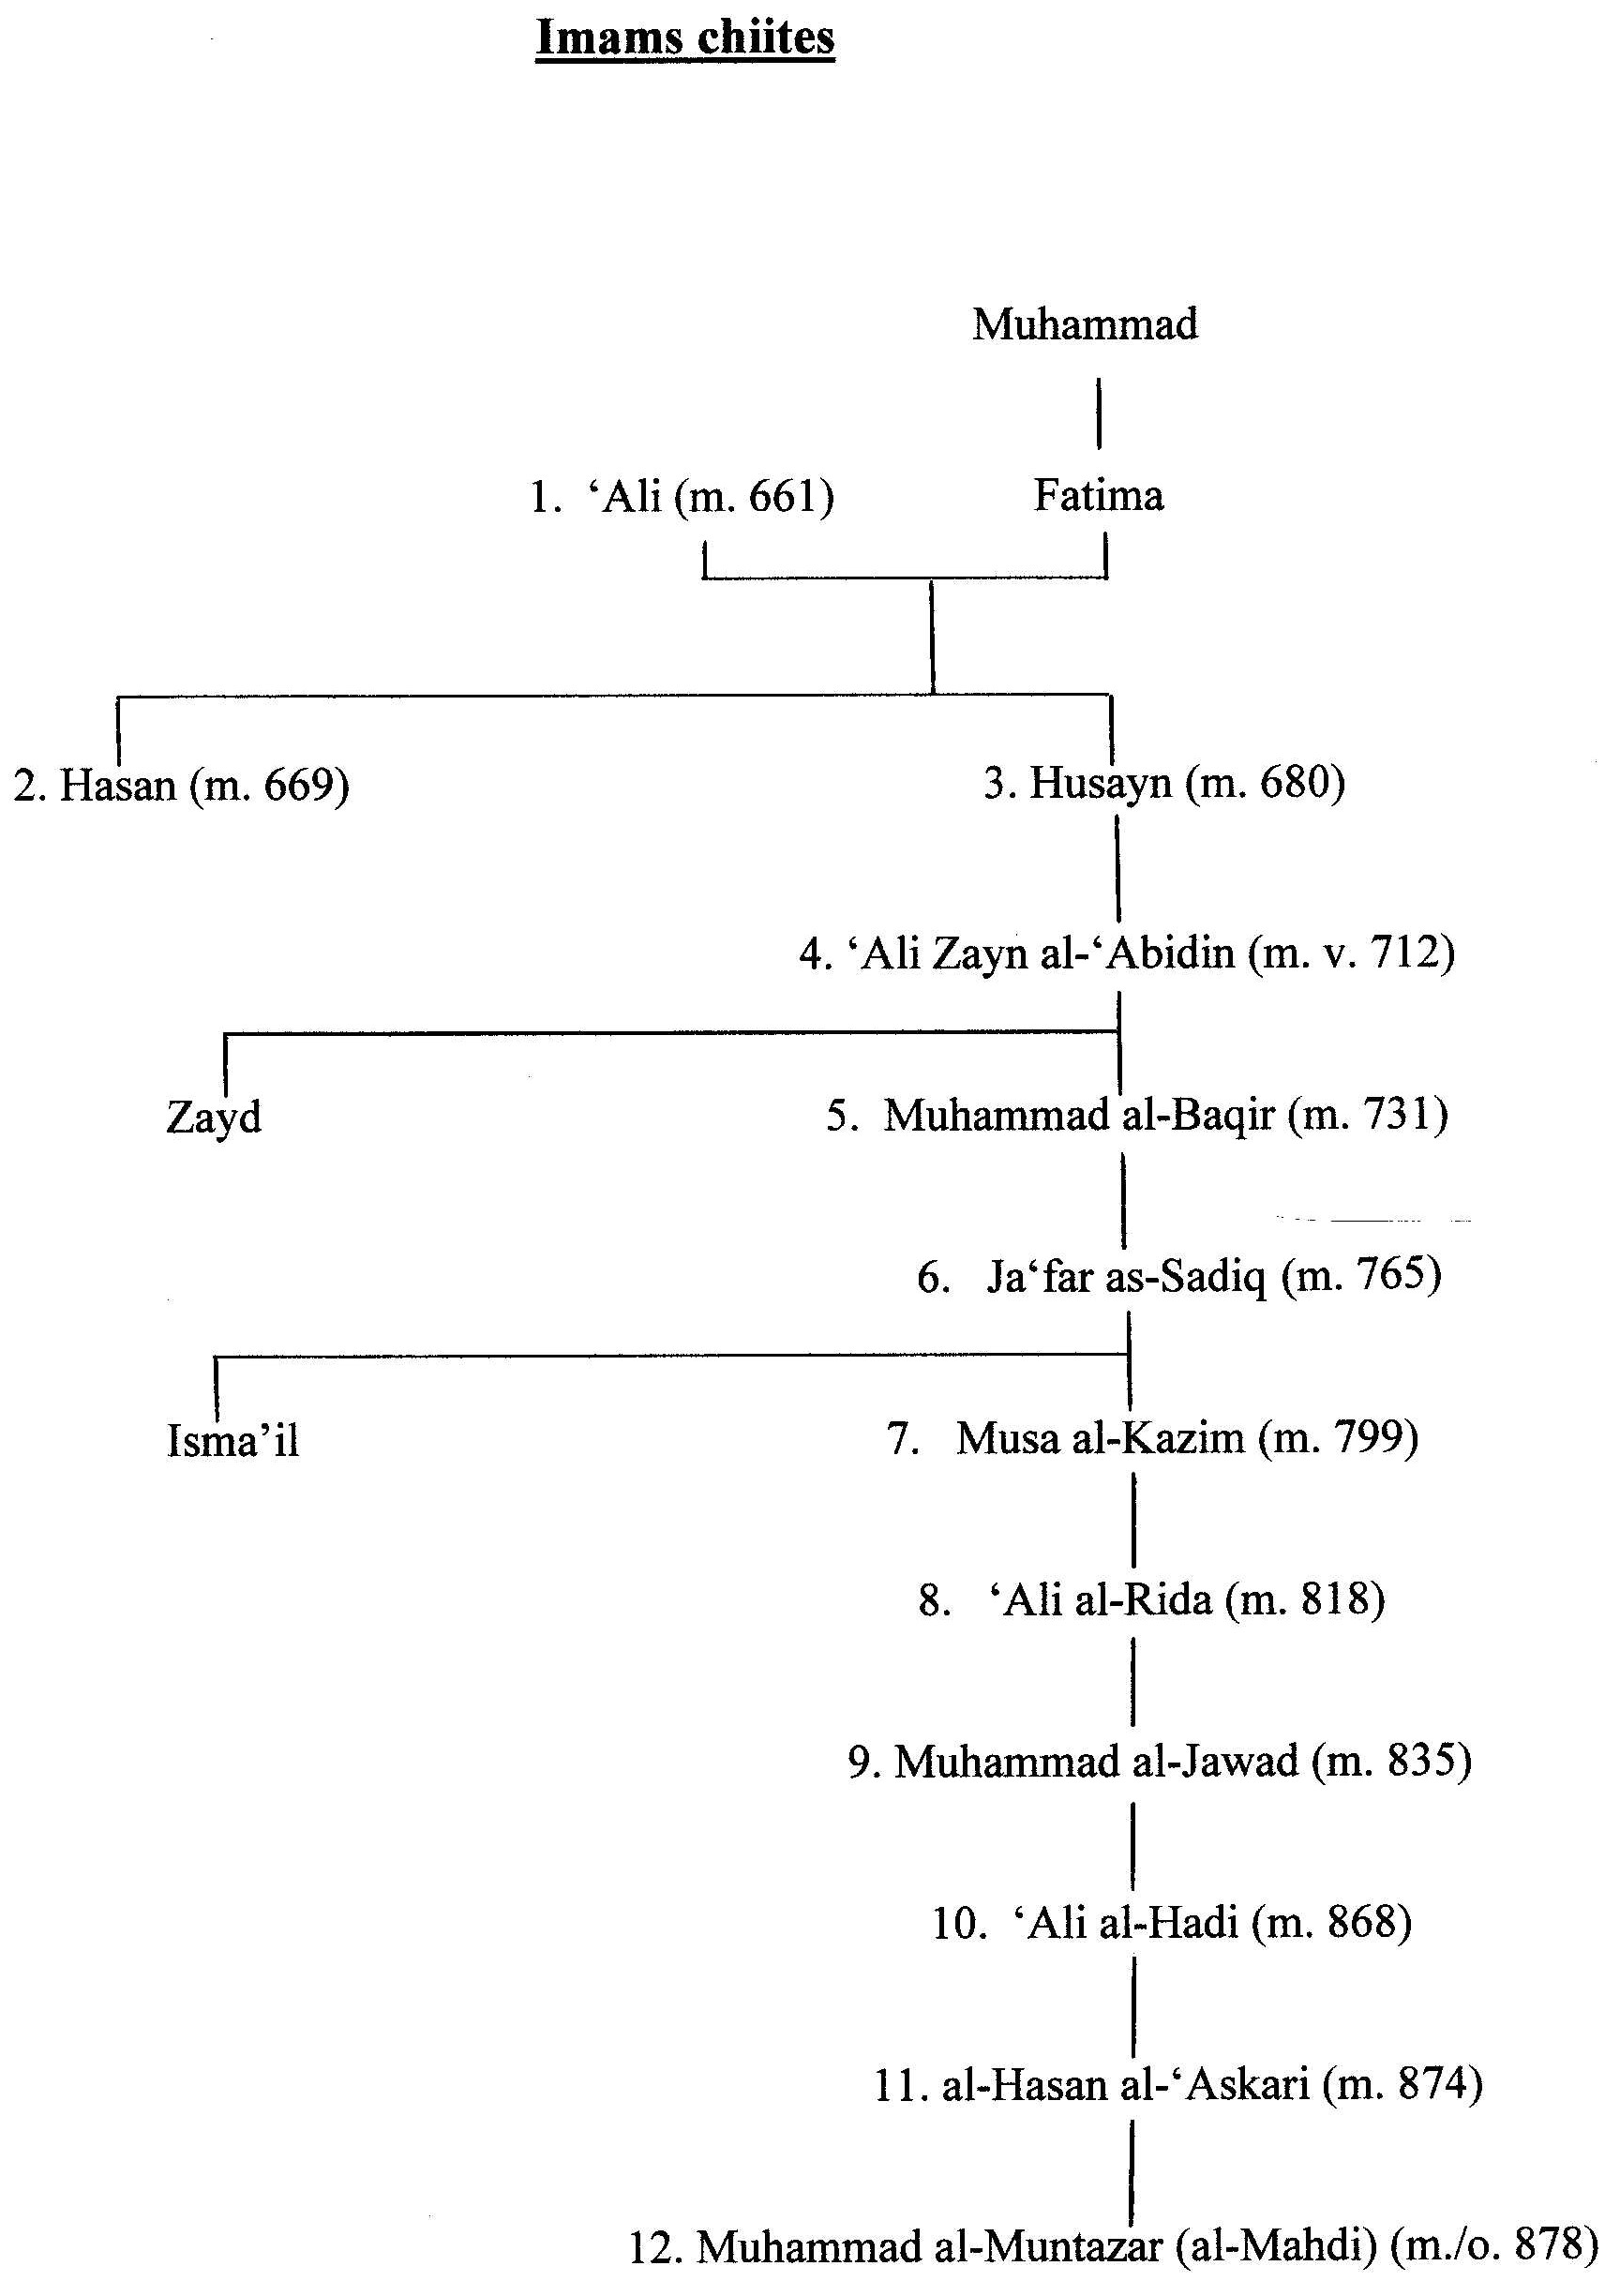
\includegraphics[width=0.8 \textwidth]{CourantsIslamContemporain/ImagesCourantsIslamContemporain/image2.png}
    \label{fig:my_label}
\end{figure}

 \paragraph{L'imam, celui qui guide} la prière et va faire le prêche du vendredi.  Dans la doctrine duodécimaine, l'imamat est lié à l'interprétation.
 Le prophète transmet la lettre du Texte. Mais elle a besoin d'être interprété : à chaque prophète dans l'humanité, correspond un imam : 
 \begin{itemize}
     \item Pour Moise, c'est Aaron
     \item Pour Jésus, c'est Pierre
     \item Pour Mohammad, c'est Ali.
 \end{itemize}
 Certes Mohammad est le dernier prophète, mais si on veut que le Coran soit parole vivante, il y a besoin d'Imams qui interprètent pour aujourd'hui la parole révélée.
 
 Du fait de problème de succession, il y a un vide à remplir (expliqué théologiquement par l'occultation), et c'est le \textit{clergé} qui le remplit \sn{Les Ayatollah ne sont pas imams. Il y a encore des imams dans le monde sunnite mais pas dans le monde chiite}.
 
 \newpage
 \paragraph{Les 14 immaculés}
    \begin{figure}
     \centering
     \sidecaption{Les 14 « Immaculés »  \newline La "Sainte Famille". \emph{Source}: Livre pour enfants iranien (Téhéran, 2006)}
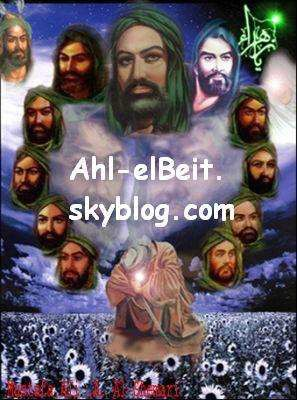
\includegraphics[width=0.45\textwidth]{CourantsIslamContemporain/ImagesCourantsIslamContemporain/Image3Chiisme.jpeg}
\includegraphics[width=0.45\textwidth]{CourantsIslamContemporain/ImagesCourantsIslamContemporain/image4.jpeg}
 \end{figure}
 
 
 \begin{Def}[les 14 immaculés]
 Les Quatorze immaculés ou Les Quatorze Infaillibles (en arabe:\TArabe{ المعصومون الأربعة عشر)} est l'expression désignant les gens de la Sainte Famille du Prophète Muhammad (s) Ahl al-Bayt, qui sont au nombre de quatorze, le premier étant le Prophète lui-même, suivi de sa fille Fâtima Zahrâ (a) et des douze Imams (a) qui lui ont succédé.
 \end{Def}
 
 
  
  
  \subparagraph{Prophétie et imamat}
  
 
Une autre tradition savante rapporte :\sn{(Source : \emph{La religion discrète}, M-A Amir Moezzi, Paris, Vrin,
2006, p. 110)}
\begin{quote}
    

« Deux mille ans avant la création, Muhammad et Ali étaient une lumière
devant Dieu -- qu'Il soit glorifié et exalté -, lumière formée d'un
tronc principal d'où partait un rayon de lumière resplendissant\ldots{}
Dieu dit alors : « Voici une lumière {[}tirée{]} de Ma propre Lumière ;
son tronc est la prophétie et sa branche, l'imamat ; la prophétie
revient à Muhammad, Mon serviteur et messager, et l'imamat revient à
Ali, ma Preuve et mon Ami. Sans eux, je n'aurai rien créé de ma
création\ldots{} C'est pourquoi Ali répétait toujours : « Je proviens de
Muhammad {[}ou de Ahmad{]} comme une clarté provenant d'une
autre\ldots{} »
\end{quote}


 \paragraph{Une science divine} pour interpréter le Coran, il y a besoin d'une science divine. L'imam a reçu une dimension spirituelle, la \textit{lumière de l'imamat}. Les imams préexistait à la création du monde en tant que réalité spirituelle. Comme les prophètes, ils sont \textit{impeccables}, sans péché.
   \subparagraph{La divinité des Imams}
De nombreux hadiths des Imams soulignent leur caractère quasi-divin : \sn{Source : « Remarques sur la divinité de l'Imam », M-A Amir-Moezzi,
\emph{Studia Iranica}, n° 25, 1996, p. 193-216}


\begin{quote}


« Hommes ! Dieu créa Ses serviteurs afin que ceux-ci Le connaissent car
lorsqu'Ils le connaissent, ils L'adorent et se libèrent ainsi de
l'adoration de tout autre que Lui ». Un homme demande alors à l'imam : «
Qu'est-ce que la connaissance de Dieu ? » « C'est pour les gens de
chaque époque, la connaissance de l'imam {[}de cette époque{]} auquel
ils doivent obéissance » (Husayn ben `Ali)

« Dieu fit de nous Son œil parmi ses adorateurs, Sa Langue Parlante
parmi Ses créatures, Sa Main de bienveillance et de miséricorde étendue
au-dessus de Ses serviteurs, Sa face grâce à laquelle on se dirige vers
Lui, Son Seuil qui guide vers Lui, Son Trésor au ciel et sur la
terre\ldots C'est par notre acte d'adoration que Dieu est adoré, sans
nous, Dieu ne saurait être adoré » (Ja`far as-Sadiq)


\end{quote}
 \paragraph{Les 14 impeccables} Le prophète, les 12 imams et Fatima. \sn{pas de difficulté de représentations dans le chiisme, depuis les enluminures persanes jusqu'à aujourd'hui. }
 
 \paragraph{le sacrifice d'Hussayn}
 
{Le martyre de l'imam Husayn}

Dans ce contexte, le martyre de Husayn, 3\textsuperscript{ème} imam, est
interprété dans les termes d'un sacrifice cosmique \sn{Source : tradition orale relevée par A-S Vivier-Muresan : \emph{Afzâd.
Ethnologie d'un village d'Iran}, Peeters, 2006, p. 48.
}:

\begin{quote}
    
 
Avant que le monde ne soit, Dieu rassembla les âmes des Quatorze
Immaculés, déjà créées, en une grande assemblée et leur annonça que,
pour ce monde qu'Il était sur le point de façonner, « du sang doit être
donné, un nourrisson et un tout jeune marié tués, une jeune femme
emprisonnée ». Aucun n'eut la force d'accepter de telles souffrances, ni
même Muhammad, ni Ali, ni Hasan. Seul Hoseyn se porta volontaire. Dieu
insista :
 

\begin{itemize}
\item
 
  Tu devras donner les tiens.
  
\item
  
  J'accepte.
  
\item
 
  Tu devras donner ta tête.
  
\item
 
  J'accepte.
  
\item
  
  Une partie de ta famille devra connaître l'exil et la détention.
  
\item
 
  J'accepte.
  
\end{itemize}


Alors Gabriel lui donna à boire la coupe de la souffrance et lui fit
signer un pacte où étaient inscrites toutes ses promesses.

Bien plus tard, lors de sa vie terrestre, approcha le temps de son
sacrifice. Il se trouvait à Karbalâ, accompagné de 72 fidèles compagnons
et de toute sa famille, encerclé par les armées de Yazid. Une armée de
djinns vint alors proposer ses services mais Hoseyn refusa : le combat
aurait été trop inégal et il se rappelait par ailleurs sa promesse. La
lutte commença et de nombreux êtres chers à Hoseyn, compagnons, fils,
frères, cousins, tombèrent l'un après l'autre sous les coups de
l'ennemi. Aveuglé par la douleur, Hoseyn en oublia sa promesse, et se
mit à tailler en morceaux l'armée adverse. Dieu s'empressa alors
d'envoyer Gabriel lui tendre le pacte qu'il avait signé au début des
temps. Rappelé à la raison, Hoseyn se soumit à la volonté divine et tint
son serment ; il retira son épée du combat et se livra à la fureur de
ses adversaires qui ne tardèrent pas à le mettre en pièces.
\end{quote}

 \subparagraph{Kerbala} la mémoire de la bataille est aussi une fête populaire. Des maquettes, repas,... le rouge reflète les partisans d'Hussayn.
 
 \begin{Def}[ta'ziyya]
\emph{représentation théâtrale du drame de Kerbala}
 \end{Def}

\begin{figure}[h!]
    \centering
        \sidecaption{Karbala}
    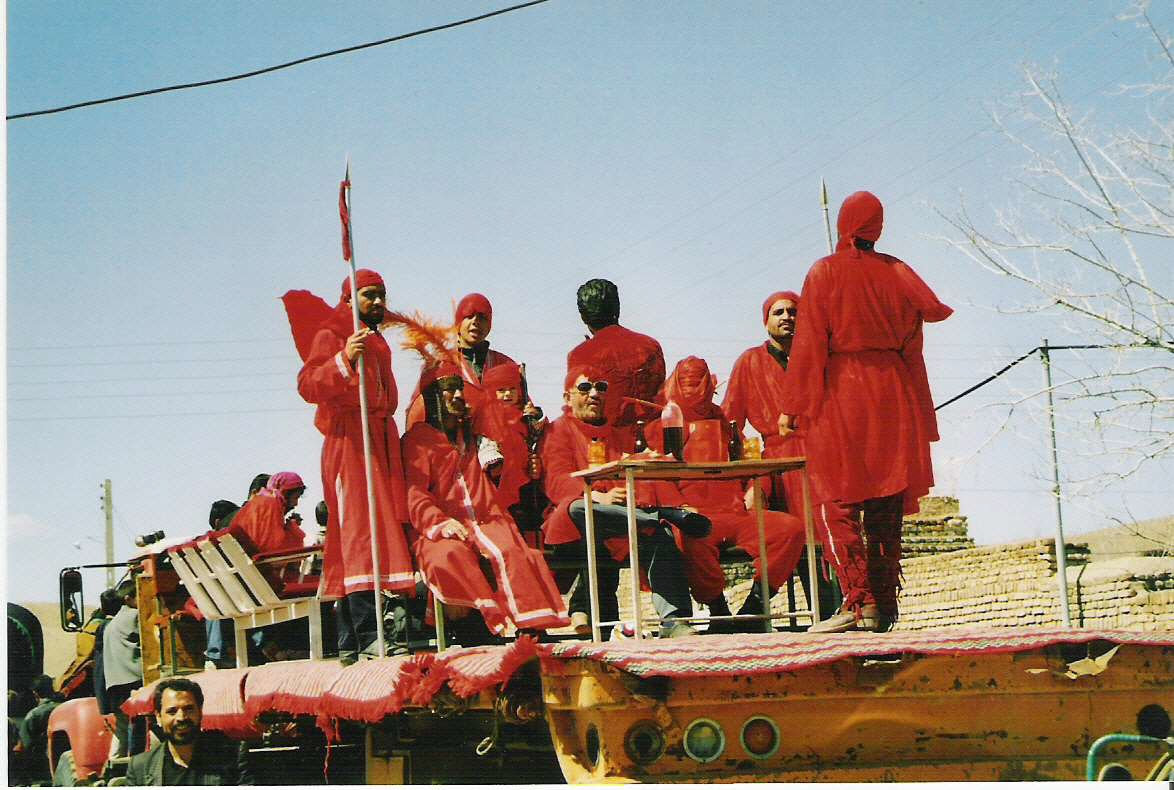
\includegraphics[width=0.3\textwidth]{CourantsIslamContemporain/ImagesCourantsIslamContemporain/image9.jpeg}
    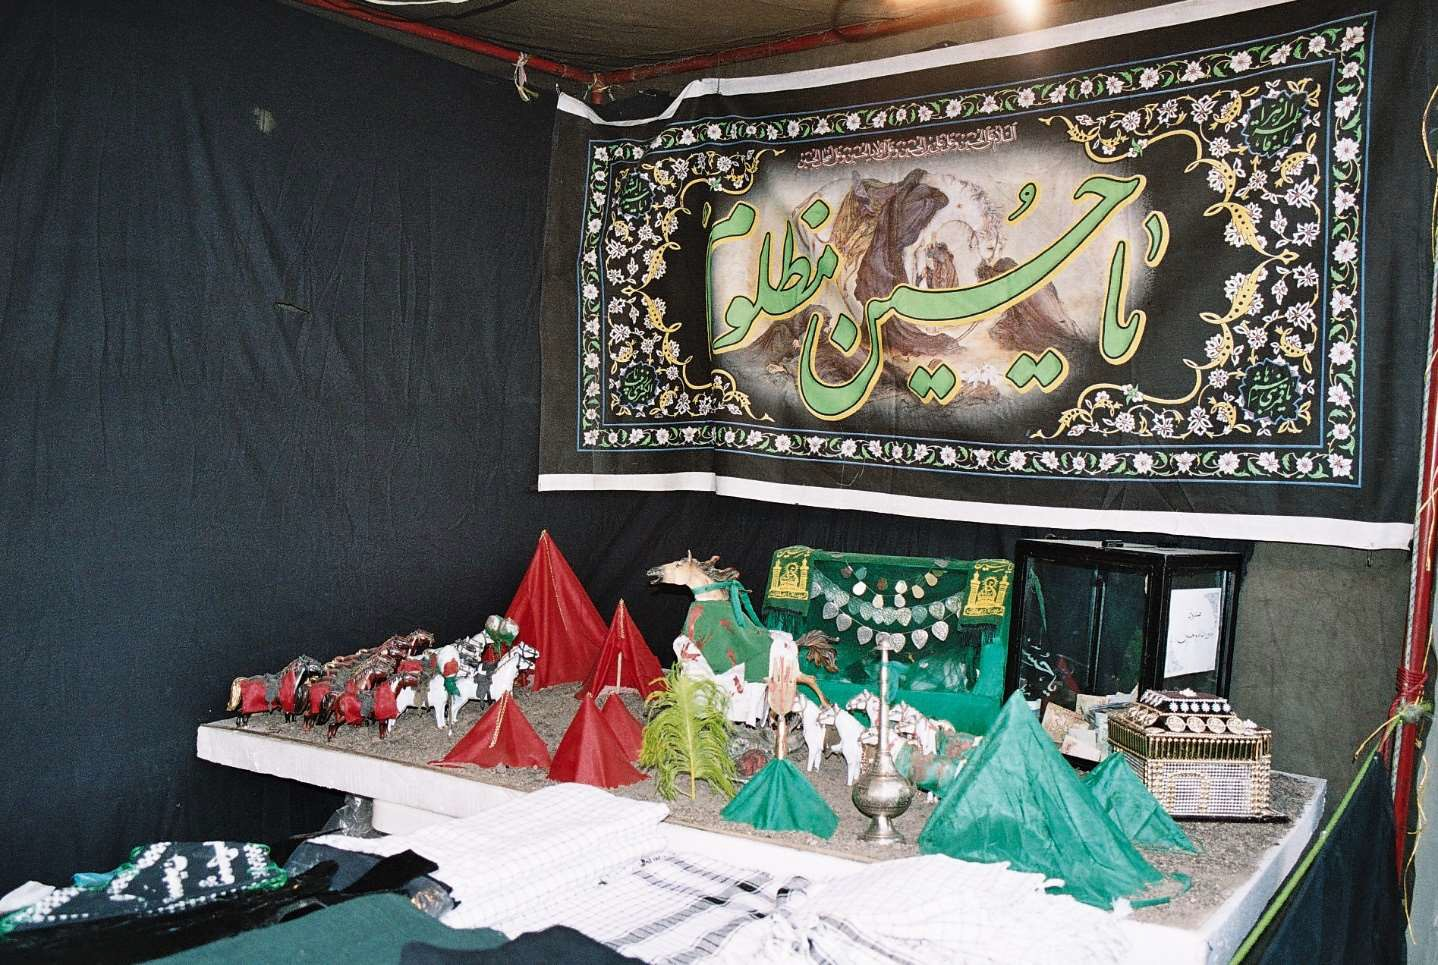
\includegraphics[width=0.3\textwidth]{CourantsIslamContemporain/ImagesCourantsIslamContemporain/image10Chiisme.jpeg}
        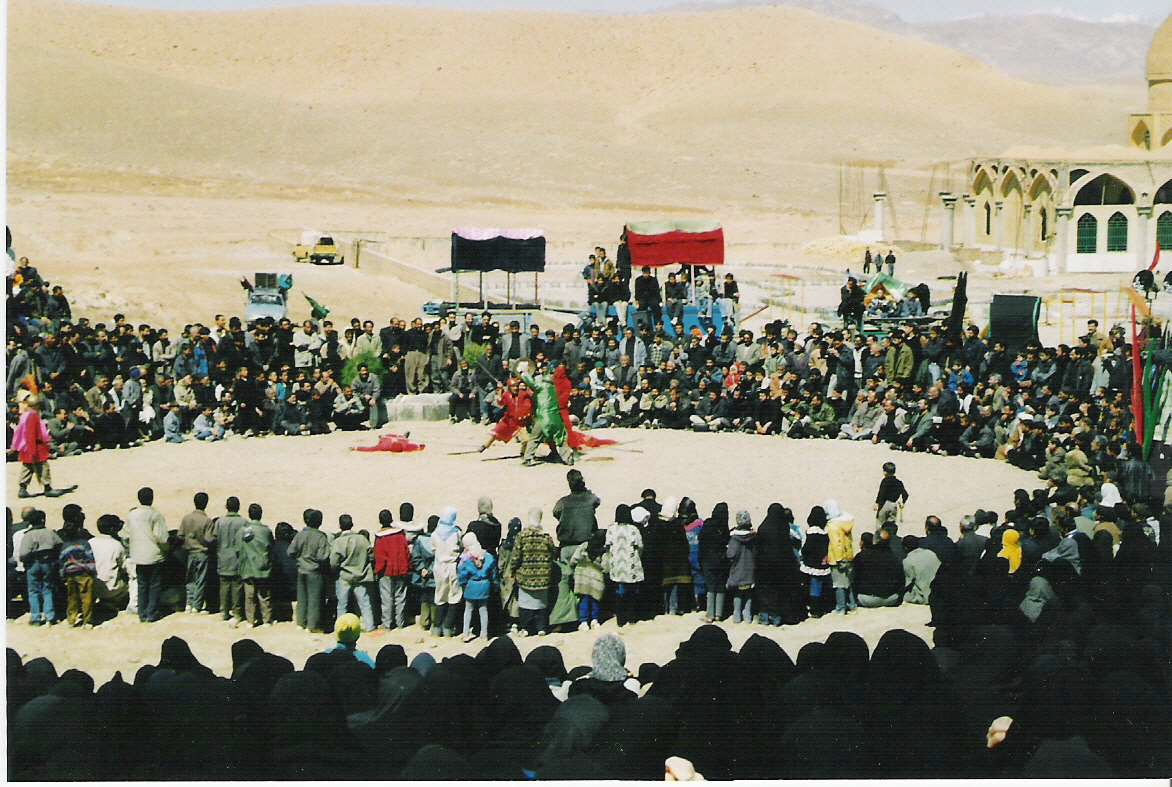
\includegraphics[width=0.3\textwidth]{CourantsIslamContemporain/ImagesCourantsIslamContemporain/image8.jpeg}


    \label{fig:my_label}
\end{figure}
 
 
 %-------------------------------------------------
 
  \subsection{Le corpus coranique et son interprétation}
 
 
  \paragraph{Le « Coran chiite »}
 
 Le Coran actuel aurait été purgé des 2/3, en particulier par tout ce qui touche 'Ali.


\begin{quote}
Certains écrits chiites rapportent des citations du «Coran intégral»
qui aurait été par la suite altéré par les sunnites. Ces citations
présentent des divergences parfois notables avec la recension
officielle, comportant souvent des mots, expressions ou bouts de phrase
absents de celle-ci (en italique dans le texte).

C. 4, 167-70 : « Ceux qui sont injustes \emph{à l'égard des droits de la
Famille de Muhammad}, Dieu ne les pardonnera ni ne les guidera sur aucun
chemin si ce n'est sur celui de la géhenne où ils y séjourneront à
jamais et c'est chose facile à Dieu.

C. 16, 24 : « Et quand on leur dit : `\,`Qu'a fait descendre votre
Seigneur \emph{au sujet de `Ali} ?'\,' Ils répondent : `\,`Fables
racontées par les Anciens'\,' » ?

C. 33, 71 : « Quiconque obéit à Dieu et à Son prophète \emph{en ce qui
concerne la walaya de `Ali et la walaya des imams après lui}, celui-là
jouit d'un bonheur grandiose ».

C. 42, 13 : « Il a établi pour vous, \emph{ô famille de Muhammad}, en
fait de religion, ce qu'Il avait prescrit à Noé, et ce que Nous te
révélons \emph{ô Muhammad}, et ce que Nous avons prescrit à Abraham, à
Moïse et à Jésus : `\,`Etablissez la religion \emph{de la famille de
Muhammad}, ne vous divisez pas à son sujet et soyez unis ».

(Source : \emph{La religion discrète}, M.A Amir-Moezzi, Paris, Vrin,
2006, p. 179-180)
\end{quote}
 
 A la fin du XIX, cette posture chiite a été abandonnée car le réformiste chiite a essayé de se rapprocher du sunnisme. De façon générale, le Coran lu en Iran a toujours été le même mais avec une suspiçion qu'il ne contenait pas tout.
 

 %-------------------------------------------------
 
  \subsection{Le rôle des clercs}
  
  \paragraph{Un sens caché du Coran, ésotérique} Seul l'imam peut interprété le Coran. \textit{"si le grand ayatolah nous dit qu'on ne doit plus prier 5 fois par jour, on le suit".} \sn{L'absence de médiation dans le sunnisme est à relativiser quand on voit l'importance pour les sunnites de ce qui est Halah et Haram et qui demandent à l'imam...}
 
 \paragraph{Les clercs vont se substituer à l'Imam} pour l'interprétation du Coran et du droit. 
 
 \paragraph{Direction de la prière} A l'époque safavide, le clerc est nécessaire pour diriger la prière. On ne peut prier collectivement sans clerc. Le clerc va s'occuper des taxes religieuses.
 \paragraph{Au XIX, déclaration du Jihaad} Alors que c'est normalement l'Imam.
 
 \paragraph{Une dernière étape, avec l'Ayatollah Khomeini, le pouvoir politique} Toutes les prérogatives normalement réservées à l'Imam.
 
 \paragraph{Un clergé très structuré}. 
 \begin{itemize}
     \item les \emph{marja} (taqlid), la \emph{source} (de l'imitation). Un fidèle doit imiter un marja. Une dizaine dans le monde. Ils se cooptent (des dynasties de Marja et d'ayyatollah). Khomeini était \textit{marja}.
     \item l'\emph{ayyatollah} qui est le seul à interpréter le Coran, une centaine dans le monde, dont quelques femmes
     \item le \emph{hojjatelislam} qui a l'équivalent d'un doctorat
     \item le \emph{mollah}, \emph{âkhund} qui dirige la prière
 \end{itemize}
 
 
 %-------------------------------------------------
 
  \section{D'autres courants chiites :
  Zaydites et
  Ismaéliens} 
 
   \subsection{Le zaydisme}
   
   Proche du sunnisme, ils reconnaissent même les trois premiers califes, ce qui est inconcevable dans le chiisme duodécimain (cf la cérémonie de bruler Omar de Khomeini).
   Environ 1 million de fidèle.
   
   \subsection{Le chiisme septimain (ismaélisme)}
   A l'autre extrême, l'imam est quasiment une incarnation de Dieu. Un primat de l'ésoterisme, occulte. Un grand rôle donné à l'initiation. Un certain recul par rapport aux pratiques, à relativiser. 

\paragraph{L'Aga Khan} chef spirituel des septimains.
 



 
\section{Glossaire}
 
\subsection{Personnes} Abbas Abu Bakr

Adud ad-Dawla Al-Karaki Hasan as-Sabah Isma'il

Kulayni (\emph{Kitab al-Kafi}) Mu'awiya (omeyyades) Nizar

Omar Osman Quraysh Yazid

{Lieux} Alamut Ardabil

Ghadir al-Khumm Jabal al-Amil Kerbala

Khorasan Kufa Machhad Sham Siffin

{Autres noms propres} akhbari

ja`farisme (école juridique chiite) kharijites

Mamlouks

Muharram (mois musulman) mu`tazilites

nizayri Qarmates Seljukides usuli

\subsection{Notions}



baten : \emph{ésotérique} (c. zaher) faqih (pl. fuqaha) : \emph{juriste}

fitna: \emph{discorde, querelle (conflit interne au monde musulman)}

ghulat : \emph{groupes chiites aux doctrines}

\emph{« extrémistes »}

hulul : \emph{« incarnation »}

ijtihad : \emph{effort personnel d'interprétation (des textes sacrés)}

`ilm : \emph{science}

imamzade : \emph{descendant des Imams / sanctuaire contenant leur
tombeau} (persan)

`isma : \emph{impeccabilité}



ma`sum : \emph{impeccable (sans péché)} mujtahid : \emph{celui qui
pratique l'ijtihad} najes : \emph{impur} (persan)

na'ib : \emph{délégué}

na'ib al-`amm : \emph{représentant général de l'Imam}

nass : \emph{élection divine}

tafsir : \emph{commentaire (exotérique) du Coran}

tanasukh : \emph{métempsychose}

ta'wil : \emph{herméneutique ésotérique du Coran} 


taqiyya : \emph{dissimulation (fait de cacher sa foi)} walayat al-faqih
(persan : velayat-e faqih) : \emph{gouvernement du juriste}

zaher : \emph{exotérique} (c. de baten)
 
 


 



 


 


\hypertarget{sabrina-mervin}{%
\section{Annexe : Les Autorités religieuses dans le chiisme duodécimain
contemporain - Sabrina Mervin}\label{sabrina-mervin}}

 \mn{
Référence électronique

Sabrina Mervin, « Les Autorités religieuses dans le chiisme duodécimain
contemporain », \emph{Archives de sciences sociales des religions} {[}En
ligne{]}, 125 \textbar{} janvier - mars 2004, mis en ligne le 22 février
2007, consulté le 17 octobre 2012. URL :
\url{http://assr.revues.org/1033} ; DOI : 10.4000/assr.1033

Éditeur : Éditions de l'École des hautes études en sciences sociales
\href{http://assr.revues.org/}{http://assr.revues.org}

\href{http://www.revues.org/}{http://www.revues.org}

}



 

En 1890, pour renflouer les caisses de l'État iranien, Nâsir al-Dîn Shah
accorda au baron de Reuter, sujet britannique, une concession qui lui
garantissait pour cinquante ans le monopole de la culture, de la vente
et de l'exportation du tabac. Aux yeux des Iraniens, c'était brader les
ressources du pays à des étrangers. La colère gronda, autant dans les
cercles cléricaux que dans les milieux bazaris et parmi la population.
Le Shah refusa d'entendre les injonctions des oulémas comme de plier
devant les manifestations populaires. L'activiste réformiste Jamâl
al-Dîn al-Asadâbâdî al-Afghânî (1), qui venait d'être exilé par le
souverain, poussa le grand chef religieux chiite de l'époque, un Persan
qui résidait à Sâmarrâ', Muhammad Hasan al-Shîrâzî, à réagir. En
décembre 1891, celui-ci promulgua une \emph{fatwâ} déclarant la
consommation de tabac illicite. Le boycott fut suivi dans tout le pays,
jusqu'au sein même de la cour du Shah, qui dut finalement plier et
annuler la fameuse concession (2).

Si le fait constitue un événement historique, traité en tant que tel par
les histo- riens de l'Iran, il est rapporté de façon récurrente par les
oulémas chiites, comme un récit exemplaire. Il leur sert à édifier les
croyants non seulement sur l'efficacité du boycott, c'est-à-dire de la
solidarité nationale, face aux compagnies étrangères, mais aussi sur
leur propre rôle dans la société, leur rapport au pouvoir, et l'étendue
de leur autorité. Ainsi, par exemple, le clerc libanais Muhsin al-Amîn
la raconta à ses amis nationalistes, à Damas, pour les encourager à
boycotter la Régie de l'élec- tricité, détenue par des intérêts
français, dans la Syrie sous mandat des années 1930. « Le Shah lui-même
ne pouvait plus fumer de narguilé, car les femmes du palais les avaient
tous fait disparaître, pour obéir à la \emph{fatwâ} d'al-Shîrâzî... »,
leur expliqua-t-il (3). Voilà pour démontrer l'efficacité de la
solidarité nationale. Quant à l'autorité des clercs, elle est corroborée
par l'anecdote suivante qui complète le récit du boycott du tabac et
circule encore, de nos jours, dans les milieux cléricaux
chiites, par écrit ou oralement. Le directeur de la compagnie
britannique voulut s'enquérir sur celui qui entravait son projet, afin
de mieux le combattre. Il demanda : « De combien d'hommes dispose-t-il ?
». On lui répondit que le clerc n'avait pas d'armée. « À combien se
monte sa fortune ? », poursuivit-il. On lui dit qu'il n'avait pas de
fortune et vivait très simplement. Le Britannique rétorqua alors que,
dans ces conditions, rien ne pouvait être tenté contre cet homme.

C'est non sans fierté que les chiites rapportent cette anecdote. Toute
l'autorité de leurs oulémas réside là : d'un mot, ils peuvent braver le
pouvoir en place, alors que le pouvoir n'a aucune prise sur eux,
puisqu'ils n'ont pas véritablement d'ambi- tion mondaine. On pense à
Khomeini défiant le Shah. Avec lui, l'autorité des clercs fut poussée à
son paroxysme, avec les conséquences que l'on sait, à savoir l'instau-
ration de la République islamique d'Iran. Certes, la figure du clerc
contestataire qui défie le pouvoir n'est pas propre au chiisme,
l'histoire de l'islam sunnite en fournit assez d'exemples, d'Ibn
Taymiyya (m. 1328) à Abd al-Salâm Yâsîn. Le premier s'en prit aux
Mongols, des envahisseurs qui s'étaient emparés du pouvoir et dont il
jugeait l'adhésion à l'islam superficielle. En outre, il blâma aussi les
soufis qui, au sein de sa propre société, s'adonnaient à des pratiques
rituelles non conformes à l'islam rigoriste qu'il prônait (4). Le second
est un cheikh marocain contemporain qui osa s'en prendre au roi Hasan II
en lui adressant un « conseil » (\emph{nasîha}). Il s'ancrait ainsi à la
fois dans la tradition islamique, qui permet au clerc d'admo- nester le
prince, grâce au principe affirmant la nécessité de commander le bien et
d'interdire le mal, et dans une tradition locale de clercs
contestataires, connue de son public. Son autorité sur les croyants fut
renforcée par le statut d'opposant poli- tique qu'il acquit suite à ce
défi, puisqu'il fut astreint à résidence surveillée (5).

Les oulémas chiites n'ont donc pas le monopole de la contestation.
Toutefois, on s'accorde à dire que, en général, les oulémas sunnites ont
eu tendance, au cours de l'histoire, à légitimer les pouvoirs en place,
alors que les chiites ont plutôt adopté une attitude de réserve à leur
égard. Au-delà des similitudes évidentes entre les oulémas des deux
grandes branches de l'islam, il importe de souligner que les chiites ont
des particularismes, autant dans le fondement de leur autorité que dans
les modalités de son fonctionnement. Pour résumer et schématiser les
processus en œuvre, on peut dire que l'autorité des oulémas sunnites,
depuis la centralisation imposée par l'Empire ottoman, l'application des
\emph{tanzîmât} et le contrôle du champ religieux instauré par les États
modernes, tend à se réduire. Alors que c'est l'inverse chez les oulémas
chiites, qui ont conquis leur pouvoir religieux et assis leur autorité
au fil des siècles et, surtout, depuis la seconde moitié du
XIX\textsuperscript{e} siècle. On va voir comment l'épisode de la
\emph{fatwâ} de Shirazi s'insère dans ce mouvement.

Selon la doctrine chiite, les douze imams infaillibles détenaient, de
leur vivant, toute forme d'autorité. En effet, les exégètes chiites
interprètent différemment des sunnites le verset coranique : « Ô vous
qui croyez ! Obéissez à Dieu et obéissez au Prophète et à ceux d'entre
vous qui détiennent l'autorité » (IV, 59). Pour les sunnites, les
détenteurs de l'autorité (\emph{ûlû al-amr}) peuvent être les califes et
les rois ; pour les chiites, ce sont les imams (6). À l'instar du
prophète Muhammad, dont ils transmirent la \emph{sunna}, les imams
étaient, pour leurs fidèles, les guides de la
communauté et les détenteurs des pouvoirs spirituel et temporel (7).
C'est pourquoi les califes et les rois qui lui succédèrent furent
considérés par les chiites comme des chefs injustes ou des oppresseurs.
En outre, dans les doctrines chiites, l'imamat fait partie des
fondements de la religion et complète la prophétie. Comme le prophète et
sa fille Fâtima, les imams sont tenus pour infaillibles : ils ne commet-
tent pas d'erreur. Par ailleurs, selon les anciens \emph{hadîth}
chiites, seuls les imams sont habilités à décliner les normes de la loi
sacrée.

Or, selon les doctrines, le douzième imam « disparut », entra en
occultation, en 874. Vivant, mais caché, il continua, dans un premier
temps, à communiquer ses prescriptions aux fidèles par l'intermédiaire
de quatre agents : ce fut la période de l'occultation mineure. Puis, à
partir de 941, il cessa d'avoir recours à des agents, et le lien avec
ses adeptes fut rompu : on entra dans la période de l'occultation
majeure, qui se poursuit actuellement. Les croyances chiites veulent
que, au terme de cette période, l'imam attendu, le Mahdî ou Qâ'im,
reviendra sur terre pour y restaurer la justice, avant la fin des temps
et le jugement dernier.

Ainsi, à partir de 941, la communauté des croyants se retrouva sans
guide, aussi bien pour les affaires spirituelles que pour les affaires
temporelles. Selon le \emph{hadîth} chiite, « Toute bannière élevée
avant le soulèvement du Qâ'im appartient à un rebelle contre Dieu
(\emph{tâghût)} », tout pouvoir politique était considéré comme inique,
illégitime (8). Or, le temps passant, il devenait de plus en plus
difficile, pour la communauté, de se passer d'autorité, de référence.
Des questions centrales restaient sans réponse : à qui verser les impôts
religieux ? Qui peut diriger la prière du vendredi ou lancer le
\emph{jihâd} ? Qui détient le pouvoir de statuer, de juger, d'arbi- trer
les conflits et de faire appliquer les peines, en l'absence de l'imam ?
Peu à peu, les oulémas procédèrent à une élaboration doctrinale, afin de
s'attribuer les fonc- tions et les pouvoirs de l'imam, et d'agir en son
nom en tant que son délégué (\emph{nâ'ib al-imâm}) (9). En outre, ils
impulsèrent un processus de rationalisation, voire d'idéologisation des
doctrines qui s'effectua par étapes successives, au moyen, notamment, de
l'introduction de différents concepts clefs. C'est ce long processus qui
allait permettre à Khomeini de concevoir sa théorie de \emph{wilâyat
al-faqîh}, « le pouvoir politico-charismatique » ou « guidance » du
théologien-juriste, sur laquelle est fondé l'État islamique en Iran
(10).

L'ouverture de la « porte de l'\emph{ijtihâd} », selon l'expression en
vigueur, est le volet principal de ce processus. L'exercice de
l'\emph{ijtihâd} consiste à extraire les pres- criptions du droit
islamique des quatre sources de ce droit, c'est-à-dire, d'une part, des
textes sacrés que sont le Coran et la \emph{sunna} et, d'autre part,
d'une série de méthodes et de techniques que l'on regroupe autour des
concepts de consensus (\emph{ijmâ`)} et de raisonnement analogique
(\emph{qiyâs}) chez les sunnites, et de raison (\emph{`aql}) chez les
chiites. C'est dire qu'il s'agit d'élaborer les normes de la loi sacrée,
la \emph{charî`a}. Le fait d'exercer l'\emph{ijtihâd} permet donc de
répondre à de nouvelles ques- tions, de réagir à de nouvelles situations
et, plus largement, d'introduire le changement dans les normes tout en
revenant aux textes. Il s'oppose au \emph{taqlîd}, le conformisme
juridique, consistant à reproduire les normes établies par les anciens.

C'est dans ce mouvement d'ouverture que réside une différence
essentielle entre l'histoire des doctrines chiites et celle des
doctrines sunnites. En effet, même si cette théorie doit être modulée et
affinée aujourd'hui, les historiens admettent que le droit islamique
sunnite est théoriquement figé, depuis la fixation de ses quatre écoles
(malékite, hanéfite, hanbalite et chaféite), au XI\textsuperscript{e}
siècle. Depuis cette date en effet, les juristes ont eu une large
tendance au conformisme, hormis les exceptions notoires de grands
savants de l'islam tels Ghazâlî (m. 1111), Ibn Taymiyya (m. 1328) ou
Suyûtî (m. 1505). Cette situation a perduré jusqu'au
XVIII\textsuperscript{e} siècle, lorsque quelques oulémas commencèrent à
prôner l'exercice de l'\emph{ijtihâd}. Puis, le mouvement s'est
intensifié, à partir de la fin du XIX\textsuperscript{e} siècle, quand
des modernistes revendiquèrent la réouverture de sa porte, afin de
mettre l'islam en accord avec l'esprit du siècle. On considère ainsi que
c'est le choc avec la culture envahissante de l'Europe qui incita des
oulémas réformistes à réagir et à entamer une réflexion sur la question.

Les doctrines chiites connurent le mouvement inverse. Alors que la porte
de l'\emph{ijtihâd} se fermait chez les sunnites, les chiites
s'employèrent à l'ouvrir de plus en plus largement et à octroyer des
pouvoirs croissants aux oulémas. Al-Tûsî (m. 1067) donna la première
impulsion à ce mouvement, que poursuivirent les savants de Hilla Ibn
Idrîs (m. 1201), al-Muhaqqiq (m. 1277), al-`Allâma (m. 1325), puis
d'autres du Jabal `Âmil (l'actuel Liban-Sud), Zayn al-Dîn al-`Âmilî dit
« le Second Martyr » (m. 1557) et son fils Hasan (m. 1602). Au même
moment, en Iran, le souverain safavide Shah Tahsmap nommait le juriste
al-Muhaqqiq al-Karakî (m. 1534) représentant de l'imâm (11). Ce courant
du chiisme duodécimain, appelé \emph{usûlî}, se renforça au
XIII\textsuperscript{e} siècle ; il devint majoritaire, et les doctrines
s'affinè- rent (12).

\hypertarget{linstitution-de-la-marjaiyya-pilier-de-lautorituxe9-religieuse}{%
\subsection{L'institution de la marja`iyya, pilier de l'autorité
religieuse}\label{linstitution-de-la-marjaiyya-pilier-de-lautorituxe9-religieuse}}

Un pas décisif fut franchi avec la systématisation de la référence à un
savant habilité à exercer l'\emph{ijtihâd}, en matière de prescriptions
religieuses. Elle fut mise en œuvre par Murtadâ al-Ansârî (m. 1864), qui
institua la fonction de \emph{marja`,} « réfé- rence à suivre », ou «
source d'imitation » pour les croyants (13). Selon cette théorie, les
croyants doivent se conformer aux avis émis par le \emph{marja`}, pour
tout ce qui concerne les questions afférant au droit islamique : d'où un
nouveau sens du terme \emph{taqlîd}, qui désigne désormais, pour les
chiites, le fait de se conformer aux prescriptions d'un \emph{marja`}
vivant, et non pas, comme c'est le cas chez les sunnites, de se
conformer aux écrits des anciens oulémas d'une école juridique donnée.
Les prescriptions, parallèlement, s'étaient élargies à tous les domaines
de la vie sociale et politique. Ainsi les oulémas pouvaient-ils
s'arroger certaines fonctions de l'imam, comme celle de déclarer le
\emph{jihâd} : ce que fit Ja`far Kâshif al-Ghitâ' (m. 1812), lorsqu'il
autorisa Fath `Alî Shah à mener la guerre sainte contre les
Russes (14). Si, par ce geste, le clerc cautionna la politique du
prince, d'autres cessèrent ensuite de composer avec le pouvoir, quitte à
s'opposer à lui. La \emph{fatwâ} que promulgua Muhammad Hasan al-Shîrâzî
fut une première étape. Après cela, des clercs s'investirent dans les
affaires politiques et, notamment, participèrent au mouvement
constitutionnaliste (1906-1911) visant à restreindre le pouvoir du Shah.

Après les travaux d'al-Ansârî, d'autres oulémas précisèrent la doctrine,
quant aux modalités du \emph{taqlîd} et aux critères de choix du
\emph{marja`}, et mirent en place le fonctionnement de l'institution.
Plus tard, des écrits tendirent à montrer qu'elle datait des débuts du
chiisme et dressèrent des listes de \emph{marja`}, à partir des plus
anciens. Même si l'idée a été reprise par des chercheurs, il s'agit bien
là d'une
« tradition inventée » (15).

Selon cette doctrine, tout croyant doit suivre les prescriptions d'un
\emph{marja`}, énoncées par celui-ci dans un traité pratique de droit
islamique, ainsi qu'à ses \emph{fatwâ.} S'il opte pour un \emph{marja`}
selon des règles établies, elles ne sont pas contrai- gnantes et son
choix s'opère donc, au bout du compte, en toute liberté. Les ancrages
ethniques, claniques, locaux et familiaux constituent bien évidemment
des facteurs influents, mais pas forcément décisifs. En outre, il arrive
que des adeptes d'un \emph{marja`} en suivent un autre, pour certaines
questions : ainsi, par exemple, dans les années 1980, bon nombre de
chiites suivaient Kho'i (m. 1992) pour les ques- tions religieuses
classiques, et Khomeini (m. 1989) pour les affaires politiques. Kho'i
étant par ailleurs très rigoriste en matière de voile, puisqu'il
prescrivait aux femmes de se cacher le visage, il leur laissait le
loisir de suivre un autre \emph{marja`,} sur ce point précis ; certaines
se référaient donc à Khomeini en la matière (16). Enfin, le croyant doit
régler ses impôts religieux au \emph{marja`} qu'il suit. Ainsi, il lui
verse la \emph{zakât}, un impôt commun aux grandes branches de l'islam,
mais aussi le \emph{khums}, spécifique au chiisme, se montant au
cinquième de ce qui lui reste lorsqu'il a dépensé ce qu'il lui faut pour
vivre.

Avec l'instauration du système de \emph{taqlîd}, un lien direct est donc
établi entre le croyant et un clerc de haut rang auquel il se réfère
pour suivre les préceptes de la loi, et ainsi assurer son salut. C'est
l'une des raisons pour lesquelles on parle parfois de « clergé »
concernant les autorités religieuses chiites qui, en outre, sont
organisées en une manière de hiérarchie. Toutefois, celle-ci est très
différente de la hiérarchie chrétienne, à laquelle on la compare
parfois, et même du système sunnite mis en place par les Ottomans, dont
se sont inspirés les États musulmans modernes.

Il n'y a aucune procédure de désignation formelle du \emph{marja`} ;
celui-ci n'est ni élu, ni désigné : on dit qu'il « émerge ». En fait,
tout se joue à trois niveaux : celui des cercles des clercs de haut
rang, celui des milieux commerçants et financiers influents, et,
\emph{in fine}, au niveau des croyants qui entérinent, ou non, les avis
des précédents. Ajoutons à cela l'influence éventuelle de l'État, sur
laquelle nous reviendrons. Le \emph{marja`} doit, d'abord, être reconnu
comme le plus savant de son temps et jouir d'une grande réputation dans
l'enseignement des sciences reli- gieuses ; c'est le premier critère de
sélection. Ensuite, il doit faire preuve de piété et de probité morale,
et être capable de percevoir les impôts et de les employer à subvenir
aux besoins des étudiants en sciences religieuses. Voilà donc les
principales qualités requises pour prétendre à la fonction, qui
s'ajoutent aux critères de bases, à savoir : être un homme, de naissance
légitime, d'âge mûr, et doué d'intelligence.

La première condition à remplir pour devenir \emph{marja`,} être « le
plus savant » en sciences religieuses, est difficile à apprécier. Aussi,
des critères plus ou moins objectifs ont été peu à peu mis en œuvre.
Avant tout, il faut compter parmi les oulémas de haut niveau, dûment
habilités à exercer l'\emph{ijtihâd} par leurs maîtres, et donc
détenteurs de certificats l'attestant. Dans les cercles de ces savants,
appelés \emph{mujtahid}, il faut être reconnu comme l'un des meilleurs.
Ce qui ne peut advenir à un jeune clerc, mais requiert âge et
expérience. En outre, la réputation du candidat se « mesure » au nombre
des étudiants qui suivent son enseignement, et à la manière dont ils le
reçoivent : s'ils prennent le soin de noter précisément les cours du
maître, et de les publier, cela ne lui donne que plus de poids. C'est
donc au sein de l'école en sciences religieuses, la \emph{hawza}, et
dans les cercles de ses pairs que le \emph{mujtahid} commence à se
distinguer. S'il répond aux incitations de son entourage à rédiger un
traité pratique de droit islamique, susceptible de devenir un guide pour
les croyants, il se pose alors en candidat à la \emph{marja`iyya}. Des
hommes d'influence (religieuse, sociale, financière) interviennent pour
le promouvoir et, au bout de la chaîne, les fidèles vont décider de se
référer à lui, ou non : l'allégeance populaire est la dernière étape.
C'est ainsi que le \emph{marja`} émerge.

Des liens étroits unissent le \emph{marja`} aux étudiants en sciences
religieuses, donc à la \emph{hawza}. Ce terme désignait d'ailleurs, à
l'origine, le cercle que forment des disciples autour d'un maître, avant
que son sens s'étende à l'école religieuse, puis au système
d'enseignement qu'elle dispense. La plus ancienne \emph{hawza} est celle
que fonda le cheikh al-Tûsî (m. 1067) à Najaf, l'une des villes saintes
du chiisme, aux côtés des autres « seuils sacrés » d'Irak, Karbala,
al-Kâzimiyya et Sâmarrâ', qui abritent des mausolées d'imams (17).
Centres de pèlerinage, ces villes saintes sont aussi des foyers de
savoir, et, particulièrement, Najaf. Celle-ci fut le siège histo- rique
de la \emph{marja`iyya}. En effet, si d'autres villes saintes ont pu, un
temps, voir émerger et abriter un \emph{marja`,} c'est Najaf qui en
compta le plus grand nombre (18). Elle est en cela désormais en
concurrence avec la ville iranienne de Qom, un ancien foyer de savoir
chiite qui fut réactivé, à partir des années 1920. Sa \emph{hawza} fut
ensuite la grande rivale de Najaf, surtout à la faveur de la révolution
iranienne qui lui permit de s'étendre et de se moderniser ; dans le même
temps, la répression qui frappait les chiites, en Irak, provoquait le
déclin de celle de Najaf (19). Après la chute du régime de Saddam
Hussein, celle-ci devrait renaître, et reprendre sa place. Toutefois,
force est de constater que déjà, le \emph{marja`} le plus suivi
aujourd'hui dans le monde chiite est `Alî Sîstânî qui, s'il est persan
d'origine, se réclame néanmoins de la \emph{hawza} de Najaf, où il
réside.

Une autorité supra-étatique convoitée

Au milieu du XX\textsuperscript{e} siècle, la centralisation de la
\emph{marja`iyya} à Najaf entraîna une organisation de l'institution. Le
\emph{marja`} de l'époque, Abû al-Hasan al-Isfahânî, systématisa le
recours à des représentants chargés d'assurer la liaison avec ses
adeptes résidant dans des zones éloignées. Les \emph{marja`} ouvrent
désormais des bureaux, partout où ils sont représentés auprès des
croyants, qui diffusent leurs écrits et leurs \emph{fatwâ}, et récoltent
les impôts religieux. Ce mouvement de centralisa- tion, qui a permis une
certaine bureaucratisation de l'institution, a oscillé avec un mouvement
de décentralisation, qui a engendré le pluralisme de l'autorité reli-
gieuse. En effet si la doctrine présente un \emph{marja` a`lâ}, ou «
référence suprême », dans l'histoire, le consensus autour d'un seul
\emph{marja`} n'a pas toujours été réalisé, et ils furent parfois
plusieurs à assurer la fonction simultanément (20). C'est le cas
aujourd'hui, où, après bien des débats et des écrits sur la question, la
tendance est non seulement à un pluralisme de fait, mais aussi à un
pluralisme souvent affirmé, et revendiqué par les acteurs. Cela, en
réaction à la tentative de centralisation iranienne opérée par Ali
Khamenei au milieu des années 1990.

Les milieux cléricaux chiites sont très attachés à l'indépendance de la
\emph{marja`iyya} par rapport à l'État, qui se fonde à la fois sur le
caractère transnational du chiisme, et sur l'organisation de
l'institution. Son autonomie financière en est un facteur essentiel.
Grâce aux impôts religieux qu'il reçoit, le \emph{marja`} finance les
écoles religieuses qui sont sous son autorité, notamment en versant les
salaires des professeurs, et en allouant des bourses aux étudiants. Il
rémunère par ailleurs ses représentants, et peut rétribuer des clercs.
En outre, il fait construire des mosquées, des \emph{husayniyya} (21),
des hôpitaux, des dispensaires, des orphelinats et autres sociétés de
bienfaisance. Les fonds investis renforcent ainsi son capital
symbolique, à savoir son prestige et son autorité religieuse. En outre,
le système permet à la \emph{marja`iyya} d'assurer la formation des
clercs et d'entretenir une hiérarchie reli- gieuse indépendante -- et,
ce, même en Iran, malgré les pressions du gouvernement islamique. C'est
une grande différence avec le monde sunnite, où les États modernes se
sont employés, en ayant recours à différentes stratégies, à contrôler la
formation des clercs et leur nomination à des fonctions religieuses
officielles (22). Certes, cela n'empêche pas la présence, en parallèle,
d'autorités autoproclamées, qui occupent une partie du champ religieux,
mais celles-ci ne relèvent alors d'aucune hiérarchie, et ont parfois des
statuts précaires. Les milieux cléricaux chiites, à l'inverse,
contrôlent et régulent le champ religieux, par le biais de la
\emph{marja`iyya}. Ce qui n'a pas manqué de susciter des tentatives de
mainmise de la part de certains États.

Ainsi, avant la révolution islamique, l'Iran essayait déjà d'influer,
d'une certaine manière, sur le choix d'un nouveau \emph{marja`.} En
effet, depuis l'accession à la \emph{marja`iyya} de Borûjerdî en 1945,
lorsqu'un \emph{marja`} venait à mourir, le Shah adressait un télégramme
de condoléances au grand clerc qu'il voulait voir lui succéder. Aussi
les chiites attendaient-ils de voir à qui serait destiné le télégramme,
pour connaître la position du souverain (23). L'avènement de la
république isla- mique changea radicalement la situation, au moins à
l'intérieur de l'Iran, puisque Khomeini assura à la fois la
\emph{wilâyat al-faqîh}, la guidance du théologien-juriste, c'est-à-dire
l'exercice du pouvoir politique, et la \emph{marja`iyya}, le pouvoir
spirituel. Toutefois, il ne l'exerça pas de manière absolue, puisque
d'autres \emph{marja`} étaient suivis, même en Iran, notamment Kho'i et
Montazeri. Pressentant, avant de mourir, que sa succession poserait un
sérieux problème, Khomeini révisa sa théorie de \emph{wilâyat al-faqîh},
de sorte qu'il opéra, \emph{de facto}, une séparation entre pouvoir
reli- gieux et pouvoir politique, même si celui-ci continuait à être
tenu par des clercs. C'est d'ailleurs la situation qui prévaut, \emph{de
facto}, dans l'Iran actuel. Ensuite, il nomma à la tête de l'État Ali
Khamenei, un clerc qui ne pouvait prétendre à la \emph{marja`iyya} car
il n'avait pas les qualifications requises en matière de savoir reli-
gieux, puisqu'il n'était même pas \emph{mujtahid}. D'autres que lui
furent donc mis en avant par la république islamique (24). Toutefois, en
1995, Khamenei fut déclaré \emph{marja`.} Face à l'opposition que
suscita cette décision, Khamenei déclara qu'il n'était pas candidat à la
\emph{marja`iyya} en Iran, mais pour le reste du monde chiite. Le
paradoxe de la situation ne manqua pas de frapper les chiites de
l'extérieur, qui se retrouvaient face à une \emph{marja`iyya} imposée
par l'Iran, alors que les sujets iraniens, eux, gardaient la possibilité
de choisir. Ils refusèrent, pour la grande majorité d'entre eux, de se
plier à cette politique d'unification et de centralisation. L'Iran dut
se rétracter et accepter de voir se développer une \emph{marja`iyya}
plurielle, qu'il pouvait tenter de circonscrire à l'intérieur, mais
incontrôlable, hors de ses fron- tières. Le cas de Muhammad Husayn Fadl
Allâh, au Liban, est très significatif : il ne s'aligna pas sur la
direction iranienne, mais s'imposa lui-même comme un \emph{marja`}
indépendant, malgré les pressions qu'il subit (25).

Le régime irakien tenta, lui aussi, de contrôler la \emph{marja`iyya}.
Comme Kho'i, puis ses successeurs, lui échappaient totalement, il promut
un \emph{marja`,} Muhammad al-Sadr, un clerc de Najaf issu d'une
prestigieuse famille d'oulémas. Ce geste fut pris par les chiites,
notamment à l'extérieur, pour ce qu'il était : une ingérence dans les
affaires de la \emph{marja`iyya}. Toutefois, peu à peu, Muhammad al-Sadr
gagna une certaine popularité, à Najaf, et prit ses distances par
rapport au régime qui l'avait mis en place. Tant et si bien qu'il en
vint à le critiquer publiquement, et le paya du prix de sa vie : après
l'avoir assigné à résidence, Saddam Hussein le fit assassiner en février
1999 (26). Depuis, ses partisans sont restés actifs et ont une assise
popu- laire, à Najaf, ainsi qu'une représentation à l'extérieur,
notamment à Sayyida Zaynab, en Syrie, où résident de nombreux réfugiés
irakiens.

Ainsi, les deux États les plus à même d'avoir mainmise sur la
\emph{marja`iyya}, et donc sur la hiérarchie religieuse chiite, ne sont
pas parvenus à l'accaparer ou à l'instrumentaliser. Reste que le fait de
l'abriter confère au moins un certain prestige vis-à-vis des communautés
chiites, et apporte une activité économique non négli- geable au pays.

L'indépendance de la \emph{marja`iyya} par rapport à l'État favorise le
caractère trans- national du chiisme, puisqu'elle réunit sous une même
autorité des réseaux d'adeptes implantés dans différents pays. Ce qui
n'empêche ni l'ancrage des chiites
dans leur région d'origine, ni leur attachement à une identité
nationale. Bien plus, le mouvement d'intégration des communautés chiites
dans les États dont ils sont ressortissants a tendance à s'intensifier.
Au plan de l'organisation des affaires reli- gieuses, le Liban a été le
premier pays (l'Iran n'étant pas à prendre en compte) à permettre à la
communauté chiite d'être représentée par une institution propre, le
Conseil supérieur islamique chiite. Le clerc qui parvint à obtenir sa
fondation en 1967, Mûsâ al-Sadr, était d'ailleurs un iranien récemment
installé au Liban. La création de ce Conseil fut un pas de plus vers la
reconnaissance d'une hiérarchie religieuse chiite interne, qui se charge
de régler les affaires de la cléricature liba- naise, tout en
entretenant des liens, en parallèle, avec la hiérarchie supra-étatique
issue du système de la \emph{marja`iyya} (27).

Enfin, l'indépendance de la \emph{marja`iyya} par rapport à l'État
implique celle de la \emph{hawza} et de la formation des clercs. La
réforme du système de l'enseignement reli- gieux supérieur chiite n'est
donc pas comparable à celle que connurent les grands établissements
sunnites comme al-Azhar, qui se modernisèrent sous la pression de
l'État. Elle se fit plus lentement, suite aux initiatives individuelles
et dispersées de grands \emph{mujtahid} ou de \emph{marja`.} Les
nouvelles générations de clercs chiites ainsi formés ne furent donc pas
promues par l'État, mais par la hiérarchie religieuse. Ce qui explique,
en partie, que les mouvements islamiques chiites sont issus de cette
hiérarchie, contrairement à la tendance prévalant dans les mouvements
sunnites.

Les oulémas chiites : modèles classiques et nouveaux acteurs

Rappelons que les fondateurs des mouvements islamistes sunnites, Hasan
al-Bannâ, Sayyid Qutb, Mawdûdî, étaient de petits intellectuels,
autodidactes en matière de sciences religieuses. Bon nombre de leurs
successeurs ont ce type de profil, même s'ils furent rejoints, ensuite,
par des clercs. Cela ne fut pas le cas des dirigeants des mouvements
chiites : une autorité religieuse autoproclamée avait peu de chance de
se faire entendre sans la reconnaissance des milieux cléricaux. Or,
s'ils sont théoriquement ouverts à tout nouveau venu, à condition qu'il
fasse ses preuves en matière de sciences religieuses et qu'il se
distingue par l'exercice de l'\emph{ijtihâd}, on constate que ceux-ci
sont peu nombreux à sortir du rang. Les grands clercs chiites forment
une aristocratie religieuse qui se reproduit à travers la \emph{hawza}.
La plupart d'entre eux appartiennent à des « familles de sciences » dont
sont issus les oulémas, depuis plusieurs générations. Ces familles
tirent leur légitimité d'une ascendance prestigieuse, un savant qui a
marqué l'histoire du chiisme, par exemple. Bien plus, certaines
proclament être des lignages descendant du prophète Muhammad, généalogie
dûment certifiée par des autorités religieuses à l'appui. Ce sont les
familles de \emph{sayyid}, dont les membres portent ce titre honorifique
et se coif- fent d'un turban noir marquant leur ascendance (28). Si,
dans les milieux sunnites, on a pu observer que suivre un enseignement
en sciences religieuses pour se former à la cléricature était une
stratégie d'ascension sociale, chez les chiites, c'est un moyen de
reproduction de l'élite religieuse (29).

Cette élite religieuse assure par ailleurs sa cohésion par une relative
endo- gamie, en prenant des femmes soit dans les familles de notables,
soit dans les familles d'oulémas. Ainsi, certaines peuvent rester
alliées par des séries d'interma- riage, sur plusieurs générations. En
outre, les affinités se renforcent par le biais des liens qui se tissent
entre le maître et son disciple, et entre des étudiants qui poursui-
vent ensemble, pendant de longues années, un cursus ardu. Fait notable,
ces familles religieuses sont souvent transnationales. La famille
al-Sadr, par exemple, qui est originaire du Liban-Sud (le lignage
apparenté y porte aujourd'hui le nom de Sharaf al-Dîn), a une branche en
Irak, et une autre en Iran.

Les dirigeants des mouvements islamiques « révolutionnaires » étaient
issus de ces grandes familles. Ainsi de Muhammad Bâqir al-Sadr, leader
du mouvement islamique irakien, exécuté en 1980 par le régime ; de son
cousin Mûsâ al-Sadr qui, venu d'Iran, s'installa au Liban où il fut
l'artisan du « réveil » de la communauté chiite avant de disparaître
mystérieusement lors d'un voyage en Libye, en 1978 ; ou bien de
Khomeini, le leader de la révolution iranienne (m. 1989). En outre,
c'étaient de grands clercs, des \emph{mujtahid} ; Muhammad Bâqir al-Sadr
et Khomeini furent même des \emph{marja`}. Ils avaient le profil attendu
pour assurer cette fonction, mais tinrent un discours novateur en la
matière. Le premier appela à une rénovation de la fonction de
\emph{marja`,} le second y apporta une redéfinition. Quant à Mûsâ
al-Sadr, il fut parmi les premiers à avoir reçu une double formation,
universitaire, à la faculté de droit de l'université de Téhéran, et
religieuse, dans les écoles de Qom et de Najaf. D'autres oulémas
iraniens, qui participèrent activement à la révolution, tel Muhammad
Beheshti, assassiné à ses débuts, en 1981, avaient ce nouveau profil.

Le modèle classique a cependant perduré. Le grand \emph{marja`} Kho'i,
qui fut le rival de Khomeini, était non seulement, comme lui, issu d'une
famille religieuse, mais il exerça ses fonctions sans vraiment
s'intéresser aux questions qui consti- tuaient le centre des débats dans
bien des cercles cléricaux, comme le rapport du religieux et du
politique, la nécessité de modernisation du discours religieux et des
institutions, etc. Alî Sîstânî, l'actuel grand \emph{marja`} qui se pose
comme son succes- seur, a la même vision, classique, de sa fonction. On
dit même qu'il ne lit pas la presse, ni ne se penche sur les affaires du
monde (30). Le fait est d'autant plus remarquable que Sîstânî est le
\emph{marja`} le plus suivi dans le monde chiite.

Pour autant, d'autres se positionnent différemment, et le revendiquent.
C'est le cas de Muhammad Husayn Fadl Allâh qui, s'il relève du modèle
classique du clerc chiite pour ce qui est de son origine et de sa
formation, a participé au mouvement islamique à partir des années 1960,
et tient aujourd'hui un discours résolument réformiste et moderniste. Il
clame la nécessité de revoir les qualifications néces- saires au
\emph{marja`} : pour lui, celui-ci doit impérativement, aujourd'hui,
avoir une bonne connaissance des affaires mondaines. On voit donc que
deux conceptions du rôle et de la fonction de \emph{marja`} se dégagent
: le modèle classique du \emph{marja`} atten- tiste, apolitique et
traditionnel ; le paradigme du nouveau \emph{marja`,} qui s'implique en
politique, se veut à l'écoute des changements sociaux, et s'engage dans
la réforme des idées et des institutions religieuses.

Le profil des générations montantes de oulémas est par ailleurs en train
de changer. Si les grands clercs en place aujourd'hui, dans le monde
arabe notamment, appartiennent encore aux anciennes familles de science,
et ont été formés à la \emph{hawza}, de nouveaux acteurs religieux
entrent en scène, suite à l'influence de l'Iran post-révolutionnaire.
D'abord, l'Iran a favorisé la vulgarisation du savoir religieux, en
ouvrant largement ses écoles, de Qom et de Machhad, notamment, aux
Iraniens et aux étrangers. Cela provoqua un décloisonnement des milieux
cléricaux, qui ont été investis par des étudiants en sciences
religieuses issus de familles non spéciali- sées dans la cléricature. En
outre, le suivi d'un double cursus, universitaire et religieux, s'est
développé ; l'Iran a favorisé le phénomène en instaurant un système
d'équivalence entre les deux. En Iran, aujourd'hui déjà, bon nombre de
clercs sont aussi des universitaires, parfois titulaires d'un doctorat ;
à l'inverse, on trouve des intellectuels issus du système universitaire
qui, par ailleurs, ont reçu un enseigne- ment religieux. On a donc des
clercs intellectuels et des intellectuels religieux. Ce phénomène
s'étend aux milieux chiites libanais et irakiens, par exemple. Dans la
\emph{hawza} placée sous les auspices de Muhammad Husayn Fadl Allâh, à
Beyrouth, la moitié des étudiants suit en parallèle un cursus
universitaire. Le directeur de l'école lui-même est un clerc, et il est
docteur en philosophie islamique.

Un « désordre organisé »

L'enseignement dispensé dans les écoles religieuses chiites a été
réformé, depuis les premières critiques formulées par des clercs contre
leur manque d'orga- nisation et de pédagogie, à la fin des années 1920.
Des oulémas parvinrent progressivement à introduire des sciences
profanes au cursus religieux, et à rationa- liser le fonctionnement des
cours, par la mise en place de programmes, de classes, d'horaires fixes.
Ce ne fut pas sans difficulté. En effet, le système de la \emph{hawza}
reposait entièrement sur la totale liberté de l'étudiant de choisir un
maître, et sur le lien qui s'établissait entre maître et disciple. Une
organisation sur le modèle des écoles profanes, modernes, allait contre
ces principes. C'est pourquoi la réforme de la \emph{hawza} rencontra
beaucoup de résistance dans les milieux cléricaux. Aujourd'hui encore,
alors que la plupart des écoles fonctionnent sur un mode réformé (plus
ou moins), des oulémas évoquent ces principes comme les garants de la
formation d'une véritable élite religieuse, non sans nostalgie (31).

Un autre principe cardinal, l'indépendance de la \emph{hawza}, est
menacé par tout processus de réforme allant dans le sens de
l'organisation des écoles et de leur bureaucratisation. L'histoire
récente en fournit un exemple frappant, celui de Kulliyyat al-fiqh, un
collège de droit islamique fondé à Najaf, en 1958. Après des années
d'hésitation due à l'opposition de leurs pairs, un groupe de clercs
réfor- mistes, Muhammad Ridâ al-Muzaffar en tête, ouvrit ce collège dont
l'organisation était calquée sur celle des établissements modernes. Bien
plus, il fut reconnu par l'État, puis rattaché à l'université irakienne.
Tant et si bien que, lors de la répres- sion contre les chiites de 1991,
le gouvernement le ferma.

C'est pourquoi, entre la nécessité de moderniser et l'attachement à un
système souple, ne reposant que sur l'autorité d'un \emph{marja`}, les
chiites oscillent sans cesse. Il
en est de même pour la réforme de la \emph{marja`iyya}. En fait,
l'institution, relativement jeune, est en perpétuel développement et
fait l'objet de nombreuses discussions, entre grands clercs. Néanmoins,
elle reste entièrement centrée sur la personne du \emph{marja`} et sur
son charisme ; celui-ci ne pouvant se charger des fonctions adminis-
tratives, il délègue ses proches, surtout ses fils et ses gendres, qui
s'occupent par exemple des investissements financiers ou de la gestion
des fondations. Tout cela fonctionne donc sur un mode patriarcal et
informel. À plusieurs reprises, il a été question de réformer la
\emph{marja`iyya} pour mieux l'organiser et la rationaliser. D'une part,
il s'agissait de revoir les modalités de désignation du \emph{marja`}
afin de les forma- liser, voire d'instaurer une direction collégiale ;
d'autre part, de mettre en place une structure susceptible d'administrer
l'institution et de la pérenniser après la mort du \emph{marja`} (32).
Autrement dit, c'était permettre un processus de routinisation. Or, ces
différentes tentatives restèrent lettres mortes, les chiites n'étant pas
prêts à se doter d'une institution qui serait comparable au Vatican,
avec un chef élu et une hiérarchie pyramidale, même si le modèle est
tentant, pour certains. Un embryon de hiérarchie a été mis en place en
Iran, notamment par la transformation de titres honorifiques, hujjat
al-islâm, ayatollâh, en grades fondés sur le degré de savoir, mais elle
est assez floue.

L'autorité religieuse chiite demeure donc dans le « désordre organisé »,
pour reprendre une expression utilisée par les clercs et les étudiants
de la \emph{hawza} (33). Cela ne signifie pas qu'elle est incontrôlée.
Si la \emph{marja`iyya} obéit toujours à des règles écrites de base,
publiées dans des ouvrages, elle est aussi soumise à des usages et à des
règles morales, plus ou moins implicites, discutées dans les cercles
cléricaux. Ainsi, par exemple, lorsque les fils d'un \emph{marja`}
prennent trop de libertés ou veulent s'arroger des fonctions revenant à
leur père, on rappelle que la \emph{marja`iyya} ne s'hérite pas, et que
les institutions fondées par le \emph{marja`} ne revien- nent pas à ses
proches, mais au \emph{marja`} suivant. Le débat doctrinal ainsi que
l'autocritique du corps des oulémas permettent de réguler l'institution
de la \emph{marja`iyya,} et laissent la porte ouverte à tout changement
d'un système voulu souple, labile, évolutif.
\chapter{Le chiisme au XXe sècle : de la Réforme à la Révolution}

\mn{28/3/22}
\section{bibliographie}



 
 
 
  KHOMEYNI, Ruhollah \emph{Gouvernement islamique}, Institut pour
  l'édition et la publication des œuvres de l'ayatollah Khomeyni,
  Téhéran, 1996.
 
 
 
  SHARIATI, Ali \emph{Histoire et destinée} {[}textes choisis{]},
  Sindbad, Paris, 1982.
 

 
\emph{Fatima est Fatima}, Albouraq, Beyrouth, 2009.

ADELKHAH, Fariba \emph{La révolution sous le voile}, Karthala, Paris,
1991.

*ADELKHAH, Fariba ; BAYART, Jean-François ; ROY, Olivier \emph{Thermidor
en Iran}, Ed. Complexes, Bruxelles, 1993.

*DIGARD, Jean-Pierre ; HOURCADE, Bernard ; RICHARD, Yann \emph{L'Iran au
XXe siècle}, Fayard, Paris, 2007.

KIAN-THIEBAUT, Azadeh \emph{La République islamique d'Iran : de la
maison du Guide à la raison d'Etat}, Michalon, Paris, 2005.

KHOSROKHAVAR, Farhad \emph{L'utopie sacrifiée, sociologie de la
Révolution iranienne}, Presses de la Fondation Nationale des Sciences
Politiques, Paris, 1993.

*KHOSROKHAVAR, Farhad et ROY, Olivier : \emph{Iran, comment sortir d'une
révolution religieuse ?}, Seuil, Paris, 1999.

MERVIN, Sabrina \emph{Un réformisme chiite. Ulémas et lettrés du Gabal
`Amil (actuel Liban-Sud) de la fin de l'Empire ottoman à l'indépendance
du Liban}, Karthala-CERMOC - IFEAD, Paris-Beyrouth-Damas, 2000.

MERVIN, Sabrina (dir.) \emph{Les mondes chiites et l'Iran}, Paris,
Karthala-IFPO, 2007.
 


\subsection{Introduction}

Le Chiisme ne doit pas être pensé en vase clos, elle est en interaction avec les pensées qui l'entoure.

\section{Le réformisme chiite}
\label{le-ruxe9formisme-chiite}

  \paragraph{Lien très fort avec au centre Najjaf et Kerbala} En terme d'influence, et de centres du Chiisme, ce sont les villes saintes de Najjaf (tombeau de Ali) et Kerbala (tombeau de Hussein). Importance du pélerinage sur leurs tombeaux. 
  Pour être plus qu'un recteur de mosquée, il faut aller à Najjaf. 
  
  
     \subsection{Un mouvement parallèle au réformisme sunnite}

  \paragraph{Le réformisme chiite} comme le réformisme sunnite, le renouveau passe par :
  \begin{Def}[tajdid] 
\emph{renouvellement}.
\end{Def}

  \begin{itemize}
      \item   l'acceptation de la modernité et la raison au centre.
      \item   Il passe aussi par une purification de la foi : \emph{tawhid}, unicité de Dieu.
      \item Cela passe par un retour aux sources, Coran et sunna (chiite)
      \item Enfin, le désir de retrouver \emph{l'umma} et refaire l'unité avec le monde sunnite.
C'est d'abord un réformisme pensé par les religieux.
  \end{itemize}

\paragraph{Al-Amin (Muhsin)} réformisme libanais.Al-Sayyed Mohsen al-Amin (b.1284/1867-d.1371/1952), also transliterated Muhsin al Amin, was a Shia scholar, biographer, traditionist, and jurist. He was born in Jabal Amil, Lebanon. His most important work is A'yan al-Shi'a.[1] \sn{\href{https://en.wikipedia.org/wiki/Al-Sayyed_Mohsen_al-Amin}{Al Amin}}

\paragraph{Baqir al-Sadr (Muhammad) Borujerdi} né le 23 mars 1875 à Boroudjerd et mort le 30 mars 1961 à Qom \sn{\href{https://fr.wikipedia.org/wiki/Seyyed_Hossein_Tabatabai_Borujerdi}{Borujerdi}}


\paragraph{Changement de l'éducation} au début du XX.

 \begin{itemize}
     \item  manuel scolaire (avec une doxa réformisme)
     \item histoire des religions, psychologie
 \end{itemize}
Ils vont se heurter à beaucoup de résistances et cela ne va aboutir qu'à moitié.


  
 
\subsection{Particularités du réformisme chiite : \emph{ijtihad, taqlid} et
    \emph{bid`a}}

Dans le sunnisme, face à l'imitation stérile des savants précédents, \emph{le taqlid}, il faut faire l'effort d'interprétation des textes du Coran (\emph{ijtihad}). On dit souvent que les portes de \emph{ijtihad} se sont fermées au XIe siècle.
Très différent dans le chiisme : 
\begin{itemize}
    \item le taqlid est positif : il s'agit d'imiter le \textit{marja}
    \item l'\textit{ijtihad} s'est toujours poursuivi par les Ayatollahs \sn{seuls eux peuvent faire l'ijtihad}. Un rapport positif à la raison dans le chiisme : On a toujours étudié la philosophie grecque. De facto, dans le chiisme, le réformisme était plutot à lutter contre l'ijtihad face à des ayatollahs considérés comme sclérosés. 
\end{itemize}

\paragraph{refus de toute médiation}Face au Wahhabisme, qui condamne toute innovation (bid'a) au titre du \textit{tawhid} et donc toute médiation (dévotion aux saints, soufisme, rôle du clergé chiite). Or la dévotion aux saints est clé dans la pratique chiite\sn{rôle économique et religieux de cette dévotion aux imams}.

    \subsection{Réforme de la doctrine et des pratiques}

\paragraph{rationalisation des imams}  On va introduire une forme de rationalisation sur les imams : pouvoir surhumain des imams, préexistence des imams,...
  au profit de leur vie exemplaire sur le plan moral qu'il faut imiter : on ne parle plus d'intercession mais du rôle de modèle.
  
 \paragraph{Schizophrénie entre une théologie épurée et une pratique } et piété populaire, qui n'a pas été condamnée et qui continue : culte des imams, voeux aux imams,...
 
 \paragraph{Des pratiques qui ont reculé} la pression de la tombe : on va sentir le poids de la terre qui va faire rejeter le lait de la mere aux ongles. Donc il y avait un vrai commerce de cadavres qui allaient se faire enterrer à Kerbala (pour éviter sa pression).
 Mais Al Amin n'a pas réussi à faire évoluer les pratiques de Achoura pour des questions de moralités (travestis, flagellation,). 
 

\section{Genèse et destin du chiisme politique : Révolution iranienne et République islamique}
\label{genuxe8se-et-destin-du-chiisme-politique-ruxe9volution-iranienne-et-ruxe9publique-islamique}


 
 
 
   \subsection{Un contexte bien particulier : l'Iran pahlavi}
    
    C'est le roi, \textit{shah} d'Iran. Au début du XX, on a une révolution constitutionnelle en 1906, qui limite (un peu) le pouvoir du Shah en introduisant une constitution.
    
    En 1921, on a la prise de pouvoir par Reza Khan, officier, dans une démarche très séculariste. Mais il décide de rester dans le cadre monarchique pour ne pas froisser les Ayatollahs. Il décide donc de créer une nouvelle dynastie, la dynastie \textit{Palhavi}.
    
    \paragraph{Des réformes sécularistes} Un réseau d'écoles publiques, modernisés. Création de tribunaux séculiers et introduit un code civil occidental, à la place du système juridique islamique qui existait auparavant.
    
    En 1935, interdiction du voile dans l'espace publique. Mais résistance à cette mesure et le voile n'est finalement interdit que dans les administrations.
    
    \paragraph{Mohammed Reza Shad (1941)} son fils au pouvoir. En 1963, il fait la \href{https://fr.wikipedia.org/wiki/R\%C3\%A9volution_blanche}{révolution blanche}, qui comporte plusieurs volets : réforme agraire, droit de vote au femme. Cela lui vaut l'hostilité du clergé (qui était grand propriétaire). Par ailleurs, il entre dans une forme de mégalomanie, notamment en 1971 (2500 ans de monarchie ininterrompue). 
    En 1975, il adopte un calendrier achéménide au lieu d'un calendrier musulman. 

    \paragraph{le clergé prend la tête de l'opposition}
    
   \subsection{Ruhollah Khomeyni (1902-1989) et le \emph{velâyat-e faqih}}
    
    \paragraph{Ruhollah Khomeyni } \sn{\href{https://fr.wikipedia.org/wiki/Rouhollah_Khomeini}{Khomeyni sur Wikipedia}} dynastie d'Ayatollahs, bourgeoisie du bazaar (commerce) et propriétaires terriens. Il est même nommé Marja en 1962. Il enseigne dans l'université de \textit{qom}. Dès les années 60, il est à la tête de l'opposition. Jugement en 1963, peine de mort commué à l'exil. 14 ans en Irak mais indispose le pouvoir irakien et s'installe en France en 78.
    
    
    \paragraph{Delégitimisation du Shah} Applique au shah, le \textit{taghut} (idole, pharaon) \sn{\begin{Def}
    [taghut] : \emph{idole ; tyran}.
    \end{Def}}. face à cette délegitimisation,  le pouvoir revient aux clercs.
    \begin{Def}[velayat-e faqih]
    le pouvoir aux clercs
    \end{Def}
    
    \paragraph{Une rupture théologique} Dans le chiisme, il y a une idée d'une corruption profonde dans le monde et qu'il n'est pas possible d'imposer le règne de Dieu sur terre. Seule le mahdi peut le faire. Face à Khomeyni, beaucoup de marjas se sont imposés à lui et à sa volonté d'avoir un rôle politique.
    
    \sn{Quand le religieux se melent de politique, c'est toujours le religieux qui est asservi par le politique.}
    
    
    
\paragraph{Le \emph{velayat-e faqih} : Ruhollah Khomeyni (1902-1989)}



\begin{quote}
    

\emph{Méthode du gouvernement islamique. Ses différences avec les autres
gouvernements.} \sn{Extraits de \emph{Pour un gouvernement islamique}, 1969 (traduction
française chez Fayolle, 1979).}

Le gouvernement islamique ne ressemble à aucun autre gouvernement
actuellement en vigueur. Il n'est pas despotique. Le chef de l'État
n'est pas un despote qui se joue des biens et de la vie du peuple et en
fait ce qu'il désire, qui tue celui qu'il veut, et enrichit ou ennoblit
qui il veut, distribuant de-ci de-là les terres et les biens du peuple.
Le Prophète, Ali et les califes n'avaient pas ce genre d'attributions.
Le gouvernement islamique n'est ni despotique ni absolutiste, il est
constitutionnel \sn{rôle de la loi : cf Banna, \textit{le Coran est notre Constitution}}, bien entendu pas au sens habituel du terme, où les lois
sont approuvées par des personnes et une majorité : constitutionnel, au
sens où les dirigeants sont tenus à un ensemble de « conditions »
définies dans le Coran et dans la Sunna du Prophète à la fois en ce qui
concerne l'exécutif et l'administration. Ces conditions ne sont rien
d'autre que les lois islamiques, celles-là mêmes qui doivent être
observées et appliquées. De cette manière, le gouvernement islamique est
le gouvernement de la Loi divine sur le peuple.

C'est ce qui constitue la différence fondamentale entre le gouvernement
islamique et les autre gouvernements constitutionnels, monarchiques et
républicains ; un autre fait capital est que dans ces régimes, les élus
du peuple ou le monarque sont les législateurs, tandis que dans l'Islam,
le seul législateur est Dieu \sn{Idéalisation de la loi islamique}, le Législateur sacré.

Personne n'a le droit d'émettre des lois, et aucune loi n'est applicable
si ce n'est celles du Législateur. Voilà pourquoi dans le gouvernement
islamique, au lieu de l'assemblée législative qui représente
habituellement l'un des trois pouvoirs, il existe une assemblée de
planification qui a pour rôle d'organiser les divers ministères au
regard des lois islamiques et de déterminer, à l'aide de ces plans et
sur tout le territoire, la manière d'accomplir les services publics.

L'ensemble des lois islamiques réunies dans le Coran et dans la Sunna
ont été acceptées par les musulmans et ceux-ci leur obéissent. Ceci
facilite la tâche du gouvernement qui devient du même coup le
coordinateur du peuple. Tandis que dans les autres régimes
constitutionnels, la majorité de ceux qui se font passer pour les
représentants de la majorité du peuple approuvent ce qui leur plaît au
nom de la loi, et ensuite s'imposent au peuple tout entier.

Le gouvernement de l'Islam est le gouvernement de la Loi. Dans cette
méthode de gouvernement, la souveraineté revient exclusivement à Dieu,
et la Loi constitue l'ordre et le décret de Dieu. La Loi de l'Islam,
Ordre de Dieu, règne d'une façon absolue sur tous et sur l'État islami-
que. Tout les hommes depuis le Prophète, jusqu'à ses califes et au
commun des mortels, sont définitivement soumis à la Loi, loi qui est
envoyée par Dieu et expliquée dans le Coran et par le Prophète. Si
celui-ci a pris la charge du califat, ce fut sur l'ordre de Dieu. Il est
Calife de Dieu sur terre et non pas calife sur sa propre initiative dans
l'intention de devenir le chef des musulmans. Lorsque des risques de
conflits se firent jour dans la communauté, étant donné le caractère
récent des conversions à l'Islam, Dieu s'est révélé au Prophète et l'a
engagé à annoncer le califat de toute urgence, ainsi, en plein désert.
Mahomet désigna alors Ali comme Calife en obéissant à la Loi, non pas
parce que celui-ci était son gendre ou qu'il avait rendu des services,
mais parce que lui-même en avait reçu la mission divine et qu'il
s'inclinait devant l'ordre divin. Dans l'Islam, le gouvernement signifie
l'obéissance à la Loi, et seule la Loi exerce son autorité sur la
société. Là où une certaine limitation des attributions a été donnée au
Prophète et aux Imams, c'est l'œuvre de Dieu. Chaque fois que le
Prophète a exprimé quelque chose ou annoncé une loi, c'était en
obéissance à la Loi divine, Loi à laquelle tout le monde sans excep-
tion doit obéir, le gouvernant comme le gouverné. Obéir au Prophète est
également un ordre de Dieu qui dit : « Obéissez au Prophète. » La
soumission aux responsables du gouvernement ou imams est également un
ordre de Dieu qui dit: «Obéissez aux Imans qui sont issus de vous.»

L'opinion des personnes, fût-ce celle du Prophète, n'a pas de prise sur
la Loi divine. Tous se plient à la volonté de Dieu. {[}\ldots{]}


\begin{Synthesis}
C'est une nomocratie, plus qu'une théocratie
\end{Synthesis}

\emph{L'Exercice du pouvoir du faqih, par les textes}

\emph{Les faqih justes, véritables successeurs des prophètes}

Dans l'un des \emph{ravâyat} les plus authentiques, il est dit : « Ali
rapporte les paroles du Prophète : Dieu ! Pardonne à mes successeurs.
(\emph{Il a répété cette parole trois fois}.) --- Qui sont tes
successeurs ?, lui a-t-on demandé. --- Ceux qui viendront après moi et
qui citeront et enseigneront au peuple mes hadith et ma Sunna. »

Par conséquent, il ne fait aucun doute que ce \emph{ravâyat} ne concerne
pas les rapporteurs de hadith, c'est-à-dire ceux qui les rédigent ; en
effet, un écrivain ne peut être calife du Prophète.

Il faut entendre par le mot calife qui est employé dans ce
\emph{ravâyat}, le \emph{faqih} de l'Islam. La diffusion des lois et
l'éducation du peuple seront à la charge des \emph{faqih} justes, car
s'ils ne le sont pas, ils ressembleront aux juges qui ont inventé des
\emph{ravâyat} contre l'Islam à la manière de Samarat Ebn-e-Djandâb.
S'il n'y a pas de \emph{faqih}, le peuple ne pourra pas connaître le
\emph{feqh}, la Loi de l'Islam. Alors deviendra possible la propagation
de milliers de \emph{ravâyat} fabriqués par les agents des oppresseurs
et les \emph{âkhond} courtisans, destinés à faire l'apologie des
sultans. {[}\ldots{]}

\emph{Les pleins pouvoirs des faqih}

Par conséquent, « les faqih sont les confidents des prophètes »,
signifie que les \emph{faqih} ont le droit de prendre en charge tout ce
qui était du domaine des prophètes. Comme ceux-ci, ce sont des hommes
qui ne doivent dévier d'aucune loi et qui sont purs et désintéressés des
biens de ce monde, comme il est dit à la fin du hadith cité plus haut :
« Tant qu'ils n'entrent pas dans le monde » (dans le bourbier de la
recherche des biens matériels !). Si donc un \emph{faqih} pense aux
biens terrestres, ce n'est pas un \emph{faqih} juste, et il n'est pas le
confident du Prophète, ni l'exécutant des lois islamiques. Seul le
\emph{faqih} juste est en mesure d'appliquer les Lois, d'établir les
principes islamiques, d'administrer les peines et les châtiments, de
veiller aux frontières et à l'intégrité territoriale de la communauté
musulmane, bref d'être le Magistrat suprême du gouvernement. Comme le
Prophète, il peut établir les principes islamiques et appliquer les
lois. {[}\ldots{]}


 
\end{quote}
    
    
    
   \subsection{ `Ali Shariati (1933-1977) et la naissance du chiisme révolutionnaire}
   
   \paragraph{Ali Shariati (1933-1977)} intellectuel laic \sn{\href{https://fr.wikipedia.org/wiki/\%27Al\%C3\%AE_Shar\%C3\%AE\%27at\%C3\%AE}{Ali Shariati sur Wikipedia}} existencialisme, théologie de la libération, marxisme,...
   Il va penser le shiisme comme \textit{la religion des opprimés}. La révolution pour imposer la justice sociale et libérer le peuple.
   \begin{Def}[musta'zafin]
   Oppression. Un concept utilisé pour les persecutions religieuses qu'Ali Shariati va appliquer au contexte socio-économique
   \end{Def}
   Fatima va être mise en avant pour montrer qu'elle est femme religieuse. Dans la société islamique, les femmes ont perdu mais ont gardé un rôle important.
   
   La grande différence avec Khomeyni,n c'est que les clercs n'ont aucun rôle : les savants ont trahis Ali et Husseyn et ont maintenu le peuple dans l'oppression.
   
   Pour Khomeyni, l'état est basé sur la loi islamique (comme Mawdudi). Alors que pour Shariati, c'est la révolution.
   
   \paragraph{Un très grand mécontentement social} Face à l'échec de la réforme agraire mal faite, un exode rural. Khomeyni récupère le discours contestataire de Shariati. 
   

   
 \subsection{ La République islamique}
     
     
\paragraph{Notion de martyr}    , de Achoura, reprise par les discours politiques de la notion de martyr. 
   En 2009, un vrai changement de ce discours puisqu'un contre-discours a appliqué Achoura,  Yazid étant le gouvernement islamique.
   
   
\paragraph{1979 : constitution islamique d'Iran}   
    
\begin{figure}[h!]
    \centering
       \sidecaption{De la République islamique d'Iran : on voit à quel point c'est verrouillé. le conseil des gardiens filtre les candidats à la présidence, peut mettre son veto aux lois}
    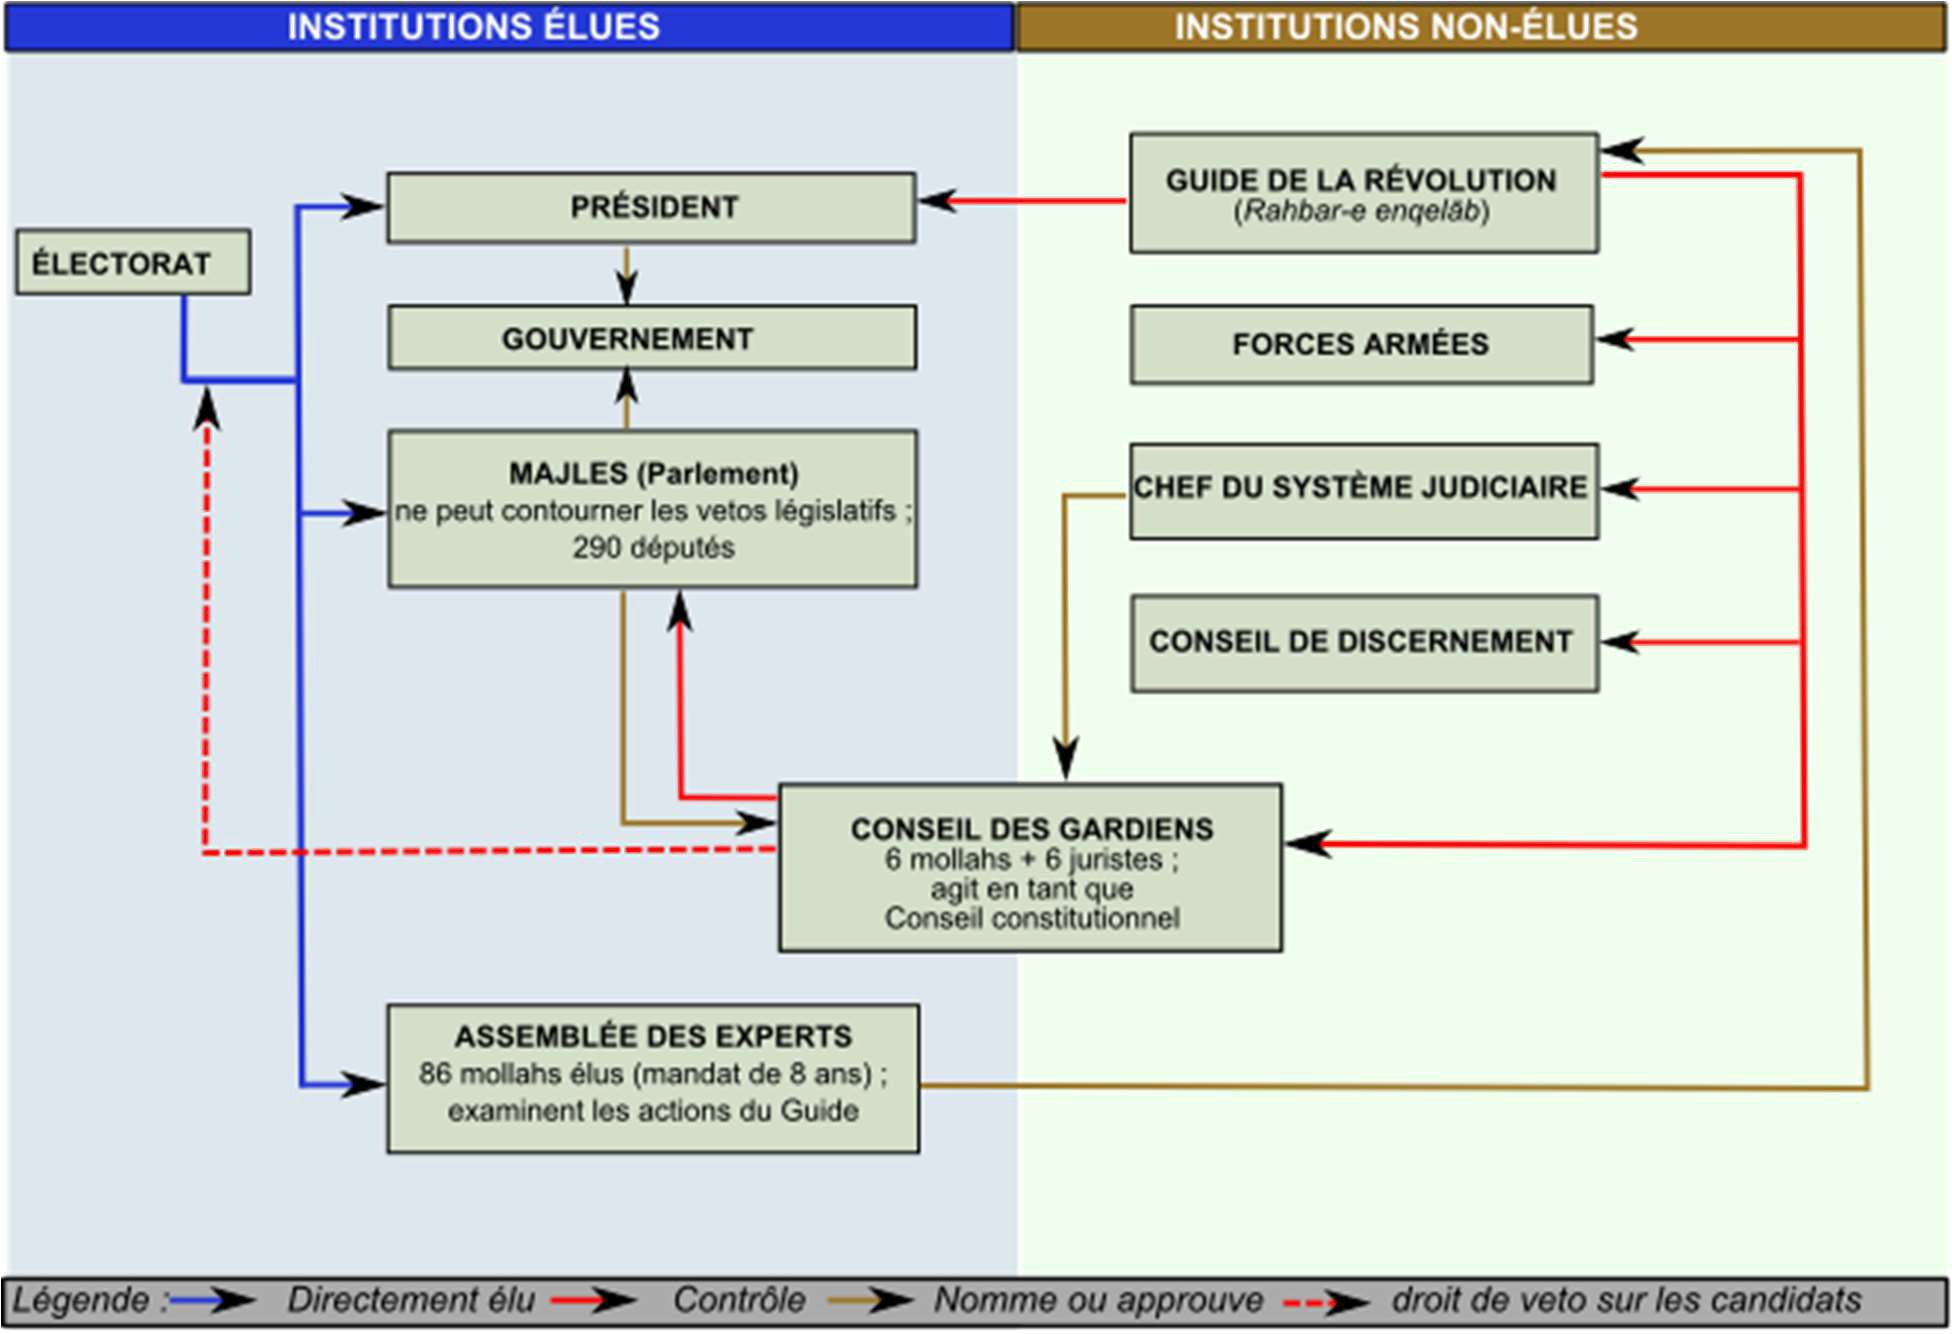
\includegraphics[width=\textwidth]{CourantsIslamContemporain/ImagesCourantsIslamContemporain/image3.jpeg}
  
    \label{fig:my_label}
\end{figure}
 

 





\hypertarget{glossaire-6}{%
\section{ {Glossaire}}\label{glossaire-6}}

 
\paragraph{Personnes}



Khameney Khatami

Khomeyni (Ruhollah) Mohammed Reza Shah Shariati (`Ali)

{Lieux} Jabal Amil Karbala Najaf

Neauphle-le-Château

\paragraph{Notions}

ayatollah : « \emph{signe de Dieu » (sur terre) ; grade supérieur dans
le clergé chiite}. marja'-ye taqlid : \emph{« source d'imitation » ;
plus haut grade dans le clergé chiite.} 



tawhid : \emph{unicité (divine).}

mujtahid : \emph{celui qui pratique l'ijtihad.}

musta`zafin : \emph{les opprimés.}





\chapter{La nouvelle pensée islamique}
\mn{\emph{(04/04/2022)}}


\section{Bibliographie}


\begin{itemize}
\item
  
  AL AJAMI, \emph{Que dit vraiment le Coran}, Erick Bonnier Editions,
  2020.
  
\item
  
  ABOU ZEID Nasr Hamid \emph{Critique du discours Religieux}, Sindbad,
  Acte Sud, Paris, 1999.
  
\item
  
  AL-BANNA, Gamal \emph{L'Islam, la Liberté, la Laïcité et le Crime de
  la tribu des « il nous a été rapporté »}, trad. D. Avon et A. Elias,
  L'Harmattan, Paris, 2013.
  
\item
  
  ARKOUN, Mohamed \emph{Lectures du Coran}, Maisonneuve \& Larose,
  Paris, 1982.
  
\item
  
  BAJRAFIL, Mohammed \emph{L'islam de France, l'an I. Il est temps
  d'entrer dans le XXIe siècle}, Ed. Plein Jour, 2015.
  
\item
  
  BENKIRANE Réda \emph{Islam, à la reconquête du sens}, éd. Le Pommier,
  2017.
  
\item
  
  CHARFI, Abdelmajid \emph{L'islam entre le message et l'histoire},
  Albin Michel, Paris, 2004.
  
\item


\emph{La pensée islamique, ruptures et fidélités}, Albin Michel, 2008.


 
\item
  
  CHEBEL, Malek \emph{Manifeste pour un islam des lumières}, Hachette,
  Paris, 2004.
  
\item
  
  ESACK Farid \emph{Coran, mode d'emploi}, Albin Michel, Paris, 2004.
  
\item
  
  LAMRABET Asma, \emph{Islam et femmes : les questions qui fâchent},
  Casablanca, En toutes lettres, 2017.
  
\item
  
  SANGARE, Youssouf \emph{Repenser le Coran et la tradition islamique --
  Introduction à la pensée de Fazlur Rahman}, Al Bouraq, 2017.
  
\item

  TALBI Mohamed \emph{Plaidoyer pour un Islam moderne}, Cérès/Tunis,
  DDB/Paris, 1998.
  

\item BENZINE, Rachid \emph{Les nouveaux penseurs de l'Islam}, Albin Michel,
Paris, 2004. FILALI-ANSARY, Abdou \emph{Réformer l'islam ? Une
introduction aux débats contemporains}, La
Découverte, Poche, Paris, 2005.

 \item HOFFNER, Anne-Bénédicte \emph{Les nouveaux acteurs de l'islam}, Paris,
Bayard, 2017.

\item RENAUD, Etienne "Mahmud Taha et la «seconde mission de l'Islam»",
\emph{Se Comprendre}, 85/07, 1985.

\item ROUSSILLON\textbf{,} Alain \emph{La pensée islamique contemporaine},
\emph{acteurs et enjeux}, Téraèdre, Paris, 2005.

\item SALEH Waël, \emph{A la recherche d'un aggiornamento de l'islam. Des
voies contemporaines}, Paris, L'Harmattan, 2018.

\end{itemize}



\section{Les nouveaux penseurs : essai
  de
  présentation}
  
  \subsection{Synthèse}
  
  \begin{Synthesis}
  Nous sommes dans un contexte Post moderne. A la différence moderne, universaliste et objectif, en post modernité, il n'y a qu'un accès relatif et subjectif à la vérité.
  Nous sommes tous des personnes raisonnables mais la façon d'accéder à la vérité, passe par le filtre de la subjectivité. 
  Le Coran passe par le filtre de la propre de subjectivité de Mohammed. Le texte est déjà une interprétation. Il y a une remise en cause du Coran \textit{Verbatim}.  
  \end{Synthesis}
  
Rachid Benzine \sn{voir p. \pageref{Theo:Benzine}}: 
\begin{quote}
    les modernistes, ou les nouveaux penseurs
\end{quote}  

Il s'est développé à partir des années 1980 en réaction à l'Islam politique et le wahhabisme, l'entrée de la violence en Islam, la cloture.

\paragraph{dans un cadre post moderne}
Ils vont chercher des nouvelles voies. La grande différence avec les modernistes, c'est qu'ils pensent la fin du XXeme. Ce n'est plus la positivité d'Auguste Comte, c'est le cadre de la post modernité. On reconnaît que la raison est construite historiquement, sociologiquement. L'accès à la vérité est donc partiel. Ce qui demeure et s'accentue, c'est la subjectivité.

\paragraph{L'herméneutique} ou Interprétation. L'accès à la vérité ne peut se faire que via l'herméneutique.

\begin{Def}[herméneutique]
Il n'y a que des interprétations à la vérité auxquelles on accède
\end{Def}

\paragraph{Conséquences} 
\begin{itemize}
    \item Il n'y a pas une essence de l'Islam. \textit{il n'y a que ce que les croyants musulmans en disent}.
    \item refus de chercher un islam pur à l'origine. Il n'y a que des islams contextualisés
    \item Importance plus faible du droit, de la norme. Ce qui compte, c'est l'éthique. L'Islam est moins pensé comme une religion normative mais un moyen pour l'individu d'entrer en relation avec le divin.
\end{itemize}

\paragraph{Rapport complexe à l'occident} Ils peuvent en particulier critiquer l'aspect absolu des droits de l'homme qu'il convient de contextualiser en Islam.

\paragraph{Un même type de formation} Plutôt formés en sciences humaines ou littératures, où ils ont découvert l'herméneutique : philosophie, histoire, ... acquis en occident. Ils prennent très au sérieux les études en sciences islamiques. 

\paragraph{En opposition avec les élites} religieuses (qu'ils critiquent) ou étatiques (face à leur souhait démocratique). Exil parfois nécessaire. En Tunisie et au Maroc, on pouvait avoir cette réflexion.

\paragraph{Du monde entier} 
\begin{itemize}
    \item Arabe
\begin{itemize} 
    \item Arkoun (Mohamed) (Algérie)
    \item Abu Zayd (Nasr Hamid) (Egypte)
    \item Khalafallah (Muhammad Ahmad) (Egypte)
\end{itemize}
\item Iran
\begin{itemize} 
    \item Sorush (Abdelkarim)
    \item Shabestari (Muhammad)
\end{itemize}
\item Pakistan
\begin{itemize} 
    \item Rahman (Fazlur)
    \item Engineer (Ali)
\end{itemize}
\item Afrique du Sud
\begin{itemize} 
    \item Esack (Farid) (théologie de la libération)
\end{itemize}
\end{itemize}
A classer : 
   Charfi
(Abdelmajid) 

 Hossein (Taha) Iqbal (Muhammad)

 

 
  
\section{Nouvelles approches critiques}

\subsection{L’approche littéraire}

Rappel du statut du Coran en Islam Classique : voix de Dieu et Mohammed n'est que l'enregistreur. Ce texte est vérité.

'Abduh va suggérer que le Coran ne doit pas être pris comme un document historique. Le but du Coran est d'exhorter les fidèles, sans avoir un soucis de précision historique.

\paragraph{Al-Khuli (Amin) 1895-1966} Enseigne à Al-Azhar. mais il a fait quelques années d'étude en Europe. Le Coran doit être compris et analysé comme un texte littéraire : 
\begin{itemize}
    \item Sémantique : les mots à l'origine. \sn{Ce n'est pas tout à fait nouveau. des les premiers siècles de l'islam, travaux sur la poésie pre-islamiques, la grammaire et dictionnaires}
    \item forme littéraire
    \item le contexte culturel et social. Cela est nouveau.
\end{itemize}

\paragraph{Khalafallah (Muhammad Ahmad) 1916-1998 } Disciple de Al-Khuli. Savant et étude de lettres à l'université du Caire (université moderne). Thèse en 1948 sur \textit{l'art du récit dans le Coran}. Il va aller jusqu'à dire que certains récits dans le Coran n'ont pas de valeur historique mais uniquement littéraire. 

\begin{Ex}
Par rapport aux récits des \href{https://fr.wikipedia.org/wiki/Sept_Dormants_d\%27\%C3\%89ph\%C3\%A8se#:~:text=Les\%20Sept\%20Dormants\%20d'\%C3\%89ph\%C3\%A8se,r\%C3\%A9cit\%20au\%20contexte\%20arabo\%2Dmusulman.}{sept dormants d'Ephèse}, va montrer que dans certains versets, il y en a 5 et dans d'autres 6. Cela montre que le but de Dieu n'est pas de faire un récit historique
\end{Ex}

Pour Khalafallah, il distingue dans le Coran différentes formes littéraires : 
\begin{itemize}
    \item Historique
    \item Parabolique : ce qui compte, c'est le message
    \item mythique (comme dans les sept dormants)
\end{itemize}

\subparagraph{une forte réaction à Khalafallah} car dès le Coran, on reprochait au Prophète de ne transmettre que des mythes. La réponse de Khalafallah a été de dire que le point du prophète était de défendre que ces textes étaient révélés. Thèse refusée et \textit{fatwa} interdisant à Al-Khuli et Khalafallah d'enseigner les sciences coraniques. Thèse néanmoins publiée.


\subsection{Critique historique}

\paragraph{Mohammed Arkoun 1928 - 2010} \label{theol:Arkoun5} En France en 1954, agrégé d'arabe\sn{cf p. \pageref{theol:Arkoun1}}. Il est marqué par la pensée des IX-X siècle. Sa compréhension de l'Islam (comme dans toute religion) : 
\begin{itemize}
    \item \textbf{la religion forte} réponse théologique crédible aux grandes questions de l'homme : le bien, le mal, ce qui se passe après la mort,... C'est ce qui compte pour toute grande religion
    \item \textbf{religion individuelle} la façon dont une religion se déploie à l'intérieur de chaque individu dans sa vie intérieure et sa relation à Dieu
    \item \textbf{la religion forme} les formes prises par la Religion dans une situation sociologiques et historiques données. Pour lui secondaire. 
\end{itemize}

\subparagraph{Une sacralisation de la religion forme} en Islam :
\begin{itemize}
    \item sur le plan politique, le \textit{califat}
    \item sur le plan politique, la \textit{shari'a}, loi religieuse
    \item et \textit{l'umma} éventuellement pouvant être pensé comme un seul état.
\end{itemize}
Si on touche à l'un de ces trois points, on touche à ce qui est considéré comme coeur à l'islam

\subparagraph{il faut une archéologie pour déconstruire ces formes}  L'Islam aurait pu être autre que ce qu'il est aujourd'hui. Ce sont des rapports de force qui ont imposé le califat, la shari'a et l'umma. 
\subparagraph{Une cloture dogmatique} au X-XI eme siècle. Ce qui est pensable et ce qui est impensable (tabou). Par exemple :
\begin{itemize}
    \item on oublie la genèse du texte du Coran. Simplification alors qu'on sait
    \item Coran incréé.
\end{itemize}
Il y a en parallèle un imaginaire, celui de l'âge d'or des 4 premiers califes, qui permet de justifier cette fermeture.

Arkoun va même jusqu'à distinguer le fait coranique de la révélation et le document historique et littéraire, le \textit{corpus officiel clos} qui est lui le résultat d'un rapport de force. 
\begin{Ex}
Osman a fait brûler des corpus hétérodoxes.
\end{Ex}


\paragraph{Différence entre les modernistes et les réformismes} Les modernistes critiquent la trahison des premières générations, à l'opposé de ce qui est reçu par la tradition musulmane d'un âge d'or.



\section{le statut de la Parole de Dieu : un Coran créé ?}



\subparagraph{Le statut du Prophète }

\paragraph{F. Rahman 1919-1988} Indo Pakistanais. Formation moderne. Inde puis Oxford (th. Philosophie). Enseigne au Canada. Rentre au Pakistan en 1961 mais il va rencontrer une très forte contestation des savants pakistanais. Ils vont l'accuser d'apostasie. Exil aux US en 1968 où il connaît une célébrité.

\paragraph{Une vision du Coran où le Coran passe par la langue et l'imaginaire du Prophète}. Voir texte. Un Coran purement extérieur du fait des controverses chrétiennes (lo-
gos,...) La parole de Dieu mais elle est aussi parole du prophète (dans
son coeur) et pas seulement enregistreur. Il reconnaît une subjectivité du
Prophète. Elle s’incarne dans son imagination, sa langue,...


\paragraph{Coran Parole de Dieu}\sn{Fazlur Rahman
(1919-1988) \emph{Extrait de son livre \textbf{Islam} (Doubleday Anchor Book, New
York, 1968, 331 pp.), p. 25-28.}}

 \begin{quote}
     

Pour le Coran lui-même, et par conséquent pour les Musulmans, le Coran
est la Parole de Dieu (kalâm Allâh). Mohammed, lui aussi, était
absolument convaincu de recevoir le Message de Dieu, le Tout-Autre (nous
essaierons plus loin de comprendre plus précisément le sens de cette
Altérité absolue), à tel point qu'il s'est basé sur la force de cette
conviction pour rejeter quelques-unes des assertions historiques les
plus fondamentales de la tradition Judéo-Chrétienne concernant Abraham
et les autres Prophètes. Cet "Autre", par un certain canal, a "dicté" le
Coran avec une autorité absolue. La voix surgissant des profondeurs de
la vie parlait distinctement, impérieusement, sans méprise possible. Non
seulement le mot \textbf{"}\emph{qur'ân}", signifiant "récitation",
l'indique clairement, mais le texte du Coran lui-même déclare en
plusieurs endroits que le Coran est révélé verbalement et non pas
seulement son "sens" et ses idées. Le terme coranique pour "Révélation"
est \emph{wahy} dont le sens est assez proche d' "inspiration", à
condition que ce mot ne soit pas censé exclure nécessairement le mode
verbal (par "Parole", bien entendu, nous ne voulons pas dire le Son). Le
Coran dit: "Dieu ne parle à aucun humain (c'est-à-dire en paroles
audibles) excepté par \emph{wahy} (c'est-à-dire par idée-parole,
inspiration) ou derrière un voile, ou bien Il envoie un Messager (un
ange) qui parle par \emph{wahy}...Nous t'avons ainsi révélé un Esprit
qui est à nos ordres". (Q. 42,51-52)


Pendant le 2° et le 3° siècles de l'ère islamique, cependant, de
violentes différences d'opinion, des controverses, en partie causées par
l'influence des doctrines chrétiennes, s'élevèrent parmi les Musulmans
au sujet de la nature de la Révélation. L'"orthodoxie" islamique
émergente qui en était au point crucial de formuler son contenu précis,
mit alors l'accent sur l'origine externe de la Révélation Prophétique
afin d'en sauvegarder son "Altérité", son "Objectivité" et son caractère
verbal. Le Coran lui-même maintenait certainement son altérité vis-à-vis
du Prophète. Il déclare en effet: "\emph{L'Esprit fidèle l'a fait
descendre sur ton coeur pour que tu sois au nombre des avertisseurs}"
(Q. 26,194), et encore: "\emph{Dis: Qui est l'ennemi de Gabriel (qu'il
le soit), car c'est lui qui a fait descendre sur ton coeur... le Livre}"
(Q. 2,97). Mais il manquait à l'orthodoxie (en fait, à toute la pensée
médiévale) d'avoir les instruments intellectuels nécessaires pour
allier, dans sa formulation du dogme, l'Altérité et le caractère verbal
de la Révélation d'une part, et, d'autre part, son lien intime avec
l'oeuvre et la personnalité religieuse du Prophète, c'est-à-dire qu'il
lui manquait la capacité intellectuelle de dire, à la fois, que le Coran
est entièrement la Parole de Dieu et aussi, dans un sens ordinaire, la
parole de Mohammed. Le Coran affirme clairement les deux idées, car s'il
insiste sur le fait qu'il est descendu sur le "coeur" du Prophète,
comment peut-il lui être extérieur ? Ceci, bien sûr, n'implique pas
nécessairement que le Prophète ne percevait pas un personnage extérieur,
comme la tradition le dit, mais il est remarquable que le Coran lui-même
ne fait aucune mention d'un personnage dans ce contexte: ce n'est qu'en
lien avec certaines expériences (habituellement liées à l'Ascension du
Prophète), que le Coran parle du prophète comme de quelqu'un ayant vu un
personnage ou un esprit ou quelque autre objet "à la lointaine limite"
ou "à l'horizon" bien qu'ici encore, comme nous l'avons dit,
l'expérience soit décrite comme étant d'ordre spirituel. Mais
l'orthodoxie, par les \emph{hadith} ou les "traditions" transmises du
Prophète, en partie interprétées correctement, et en partie inventées,
ainsi que par une discipline théologique largement basée sur le
\emph{hadith}, fit de la Révélation prophétique un phénomène ne frappant
que son oreille, uniquement extérieur à lui, considérant l'ange ou
"l'esprit qui vient sur le cœur" comme un agent totalement externe.
L'image que l'Occident moderne garde de la Révélation prophétique se
base largement sur cette formulation orthodoxe plutôt que sur le Coran,
d'ailleurs la foi du Musulman ordinaire fait de même.

... Lorsque la perception intuitive de la morale chez Mohammed atteint
son plus haut point et s'identifie avec la morale elle-même, la Parole
est donnée avec l'inspiration elle-même. Le Coran est donc la pure
Parole divine, mais évidemment, il est également relié intimement à la
personnalité interne du Prophète Mohammed, dont la relation au Coran ne
peut être conçue mécaniquement comme un disque enregistré. La Parole
divine passe par le cœur du Prophète.
 \end{quote}


\begin{Synthesis}
Un Coran purement extérieur du fait des controverses chrétiennes (logos,...)
La parole de Dieu mais elle est aussi parole du prophète (dans son coeur) et pas seulement enregistreur. Il reconnaît une subjectivité du Prophète. Elle s'incarne dans son imagination, sa langue,...
\end{Synthesis}

\subsection{L’ « abaissement » de la Parole }
\paragraph{Abu Zayd (mort en 2010)} Littérature arabe en Egypte et étude aux USA. Approche littéraire. Une langue est forcément porteuse d'une culture donnée, une langue particulière. Il va jusqu'à parler d'une \textit{incarnation de la Parole}, une langue humaine. Si Dieu a choisi l'arabe, il faut étudier ce texte en Arabe comme n'importe quel texte littéraire. 

\subparagraph{Contextualisation culturelle}

\section{la question de l'interprétation}

\subsection{Approche littéraire} 
Avec Abu Zayd.
Tout texte demande à être reçu et interprété, il ne vit pas en soi. C'est le passage, la transformation par la subjectivité de l'auditeur. Et ce texte coranique est \textit{marqué par l'interprétation du Prophète}. Il va comparer le Coran à un organisme vivant qui est riche d'une infinité de sens et qui va se donner selon la compréhension de l'auditeur.

\paragraph{des critères pour interpréter}


\begin{itemize}
    \item Sens : sens qu'avait le texte pour le prophète et ses compagnons
    \item signification : sens pour aujourd'hui
\end{itemize}
Le critère est de s'assurer de la \textit{cohérence entre sens et signification}. 


\subsection{Approche scientifique }

\paragraph{A. Sirush 1945-} Approche par la philosophie des sciences. Il a découvert la philosophie des sciences; Thèse en Angleterre. Très enthousiaste au début de la révolution en Iran. Il s'est exilé aux US (Harvard).

\paragraph{Un parallèle entre nature/science et religion} A. Sirush fait un parallèle entre nature et science d'une part et Religion et ce qu'il nomme religiosité d'autre part:
 
\begin{tabular}{p{5cm}p{1cm}p{5cm}}
Nature &  & Religion   \\
\textit{{objectif, absolu} }      \\                        
          $ \downarrow $  &  &         $ \downarrow $  \\
Science &  & Religiosité\\
\textit{{partielle, mouvante}}  & & \textit{ce que nous comprenons de la religion} \\
\end{tabular}
 


\paragraph{théorie de l'extension et de la contraction de la connaissance religieuse}, la religiosité. Tout est lié, toute découverte sur les sciences a un impact sur notre philosophie et l'anthropologie, et donc ensuite sur notre compréhension.


\begin{Ex}
L'Eglise s'est opposée à l'idée que la terre tournait autour du soleil. Car cela changeait notre regard de la place de l'homme et de la création, au centre et au sommet de la Création.
\end{Ex}

\paragraph{un processus continu} de connaissance religieuse. Notre compréhension de la religion évolue. Il faut être dans une attitude de questionnement pour que le Coran parle. 
\begin{quote}
    Si l'homme n'a aucune question à poser au religieux, il ne vient apprendre de ce religieux. \ldots Même chose pour le Coran.
\end{quote}

\paragraph{Pluralisme de pensée}
Cela a des implications politiques et démocratiques. Dialogue.

\subsection{Glossaire}

 
{Personnes}



{Notions}
\begin{Def}[tafsir]
\emph{commentaire (exotérique) du Coran}
\end{Def}


\begin{Def}[ta'wil]
\emph{herméneutique ésotérique du Coran}
\end{Def}
 


\chapter{Evolution de l'interdiction du \riba et Gharar}


a. Un dossier sur un thème lié au cours A partir de trois articles universitaires minimum. -  Introduction : intérêt du thème au regard de l’actualité et/ou de vos propres orientations personnelles ; présentation des articles et de leurs auteurs. Présentation du plan de votre travail. - Synthèse (ne pas présenter les articles séparément mais faire une synthèse à partir des différentes thématiques rencontrées) - Contextualisation de ce thème dans l’islam contemporain, éclairage par le contenu du cours (enjeux, dynamiques, etc). 

\section{Introduction}

En tant que membre du jury de l'Institut des Actuaires, j'ai eu à me prononcer sur certains mémoires présentés par des étudiants sur la \textit{finance Islamique} et \textit{l'assurance Takaful}. Ces mémoires ne couvrent pas les présupposés théologiques et commencent généralement par une présentation des interdits de la loi musulmane, comme par exemple ce \href{http://www.ressources-actuarielles.net/EXT/ISFA/1226-02.nsf/0/8c814ff5f2bae57ec1257e1a004407b6/\%24FILE/Memoire_ISFA_Tontines_et_Takaful_Bendimerad_Version_avec_Couverture.pdf}{mémoire d'actuariat} : 
\begin{quote}
     [pour faire face à ses  engagements, l'assureur],peut, par exemple, inclure des actifs obligataires dont les taux de rendement font apparaître des taux d'intérêt. [...] l'interdiction de l'usage du taux d'intérêt, appelé \textit{\riba} en arabe, est l'un des fondements du droit des affaires musulman.
\end{quote}
Dans la même veine, sont généralement définis les autres interdits, comme le \emph{Gharar}, défini dans le même mémoire comme : 
\begin{quote}
    Le contrat d'assurance peut constituer une perte disproportionnée en faveur de l'un des participants aux dépens de l'autre. Ce caractère d'incertitude, appelé \textit{Gharar} en arabe, est un caractère prohibé par l'Islam surtout lorsque le transfert du risque vers un tiers est total, ce qui est notamment le cas pour l'assureur qui porte entièrement la charge du risque cédé par l'assuré.
\end{quote}
Les mémoires d'actuariat consultés essayent de dépasser ces interdictions, qui soulignent une tension avec les \textit{Hadiths} : 

\begin{quote}
     
A l'issue de l'analyse précédente, l'idée même d'une assurance islamique semble être un contresens. Pourtant, la religion musulmane encourage l'individu à prendre des mesures pour réduire l'ampleur des désastres qui pourraient l'affecter. D'après un Hadith authentifié, le prophète conseille à un croyant de placer sa confiance en Dieu et d'attacher son chameau plutôt que de se limiter uniquement à placer sa confiance en Dieu en offrant la possibilité au chameau libre de s'échapper. L'Islam ne s'oppose donc pas à l'idée de vouloir minimiser les risques et par conséquent elle ne s'oppose pas à faire usage de la loi des grands nombres. Elle exclut certes la spéculation et l'incertitude ainsi que le taux d'intérêt. En revanche, elle compte parmi ses principes la coopération et l'entre-aide mutuelle ainsi que le partage équitable des risques et des bénéfices. Toutes ces bases ont permis de concevoir un modèle alternatif à celui de l'assurance conventionnelle.
\end{quote}
De cette tension naît des solutions techniquement assez complexes.


Intrigué par cette apparente clarté vis à vis de l'interdiction de l'\textit{intérêt} et de l'\textit{l'incertitude} à la base de l'économie moderne, je me propose d'étudier l'évolution de l'opposition de la \emph{\riba} et \emph{gharar} dans les différents courants de l'Islam contemporain, depuis la pensée d'Abduh jusqu'aux frères musulmans et le salafisme. 
L'interdiction des deux notions n'a pas la même importance économique et la \textit{\riba} a donné lieu à plus de développement. En partant de ces études, j'essayerais néanmoins de transposer ces travaux à l'assurance.
Après avoir regardé  à travers l'étude de ces deux notions comment l'économie moderne, pensée au XVIIIè et XIXè siècle questionne l'Islam, je poserai quelques pistes sur le propre questionnement du Christianisme. Après tout, le prêt à intérêt était aussi interdit au Moyen-äge en Europe (Concile de TOurs de 1163). Ces pistes seront en particulier nourries par l'étude de la pensée de Saint Thomas d'Aquin sur les taux d'intérêt et comment ces pistes peuvent nourrir la réflexion de la théologie musulmane (et chrétienne) contemporaine. 
 

%---------------------------------------------------------------------------------------------------------------
\section{Vision dans l'Islam Classique de l'interdiction de \riba}

\subsection{une interdiction de la \riba et Gharar}

Pour commencer, il est utile de se référer aux textes à l'origine de ces interdits.
\paragraph{Versets du Coran et Hadiths interdisant la \riba}
Le verset 130 de la Sourate 3, Al-Imran mentionne : 
\vocalize % switch diacritics for short vowels on
\transtrue % display the transliteration
\arabtrue % print arabic text (on by default)
\begin{quote}
 
\TArabe{
 يَا أَيُّهَا الَّذِينَ آمَنُوا لَا تَأْكُلُوا الرِّبَا أَضْعَافًا مُّضَاعَفَةً وَاتَّقُوا اللَّهَ لَعَلَّكُمْ تُفْلِحُونَ
  } 
   [3,125] O vous qui croyez !, ne vivez pas de la \textit{\riba} [produisant le] double deux fois ! Soyez pieux envers Allah ! Peut-être serez-vous bienheureux. 

\end{quote}
\begin{quote}
\TArabe{278
 يَا أَيُّهَا الَّذِينَ آمَنُوا اتَّقُوا اللَّهَ وَذَرُوا مَا بَقِيَ مِنَ الرِّبَا إِن كُنتُم مُّؤْمِنِينَ
279 فَإِن لَّمْ تَفْعَلُوا فَأْذَنُوا بِحَرْبٍ مِّنَ اللَّهِ وَرَسُولِهِ وَإِن تُبْتُمْ فَلَكُمْ رُءُوسُ أَمْوَالِكُمْ لَا تَظْلِمُونَ وَلَا تُظْلَمُونَ
} 
 [2, 278] O vous qui croyez !, soyez pieux envers Allah ! Faites abandon de ce qui [vous] reste [à toucher provenant] de la \textit{\riba}, si vous êtes croyants !
[2, 279] Si vous ne le faites point, attendez-vous à une guerre de la part d’Allah et de Son Apôtre ! si vous vous repentez, alors vous récolterez votre capital sans infliger ou être victime d’une injustice. \sn{Traduction de Blachière, sauf la dernière phrase \cite{ElGamal:BanqueFinanceIslamique}}

\end{quote}

De même, un hadith de Abu Hurayra met au même niveau la \textit{\riba} et le meurtre : 
\begin{quote}
    "Evitez les sept turpitudes !"

- "Quelles sont-elles, ô Envoyé d'Allah?", demandèrent les fidèles.


- "Ce sont, répondit-il :

 

-le polythéisme,

-la magie,

-le meurtre qu'Allah a interdit sauf à bon droit

-l'usurpation des biens de l'orphelin,

-la \textit{\riba},

-la fuite du front au jour du djihad et

-la fausse accusation (de fornication) des femmes vertueuses, chastes et croyantes".
\end{quote}
 
  Nous avons évité à ce stade de traduire le terme de \textit{\riba}, par \textit{usure} ou \textit{intérêt}. Le Hadith rapport par at-Tirmidhî a été utilisé pour appliquer le sens d'intérêt à la \textit{\riba}  : 
 \begin{quote}
     Vendez de l'or contre de l'argent (les quantités échangées étant) comme vous voulez, à condition que ce soit main à main. Vendez du blé contre des dattes sèches (les quantités échangées étant) comme vous voulez, à condition que ce soit main à main. Vendez de l'orge contre des dattes sèches (les quantités échangées étant) comme vous voulez, à condition que ce soit main à main (n° 1240)
 \end{quote}  
 On peut effectivement y lire le refus de l'intérêt mais d'autres lectures sont possibles, en particulier en relevant l'insistance du hadith à une transaction \textit{main à main}, qui permet une transaction claire. Par ailleurs, la valeur du temps n'est pas explicitement mentionnée.
 

 
\subsection{un nouveau contexte avec la naissance du Capitalisme}
Du point de vue du prêteur, le prêt à un prix du fait du risque  que l'emprunteur repaye le prêt, la valeur temps (qui correspond à l'inflation et à la perte d'opportunité d'un investissement aujourd'hui qui rapporte plus plus tard). La pertinence économique de l'intérêt et de la prise de risque est donc justifiée même si cela ne veut pas dire qu'elle l'est d'un point de vue religieux.
Avec l'accumulation des richesses dans les villes italiennes au moyen-âge naît le capitalisme et la finance : comment financer et assurer les bateaux partant de Gênes et remplis de richesse ? Cette irruption de la finance pose de nouvelles questions.  Face à cette accumulation, une réponse théologique chrétienne sera la création de l'ordre mineur par Saint François d'Assise. Et, nous reviendrons sur ses développements, la réflexion de l'université de Paris et de Saint Thomas d'Aquin sur la notion d'usure et de juste prix.  
Ces innovations touchèrent tardivement le monde musulman, au XIXème, avec l'arrivée simultanée de l'industrialisation, qui nécessite des capitaux importants et les débuts de la colonisation. Par l'industrialisation, la capacité productive est fortement augmentée par l'investissement, mais aussi la concentration des risques qui ne peuvent être portée par la solidarité traditionnelle.
Face à cette nouvelle question, quelles sont les réponses proposées par les théologiens musulmans depuis l'arrivée de cette question ?


%---------------------------------------------------------------------------------------------------------------
\section{Elements théologiques apportés}

\subsection{Premières réponses face à la nécessité du prêt}
\paragraph{Le développement du \riba et de l'assurance par les Occidentaux} Les prêts à intérêt ont toujours existé au sein de l'Empire Ottoman\cite{Gilbar:Qadi}, et proposés par des familles grecques, arméniennes ou Juives (et en Iran par les arméniens et zoroastriens). A ce premier Groupe, s'ajouta les banques commerciales européennes ou les banques "étrangères-locales" comme la banque impériale ottomane au XIX.
De la même façon pour les assurances, Ibn Abidin, représentant de l'école officielle de droit Hanadi dans l'empire ottoman, suggère le compromis suivant : il est licite d'établir ds contrats d'assurance portant sur les risques encourus à l'intérieur du royaume islamique - le Dar al Islam -à condition que ces contrats soient conclus avec une compagnie d'assurance ayant son siège hors de pays de l'Islam. 

\paragraph{Utilisation de prêt à intérêt par les musulmans malgré l'interdiction du \textit{\riba}.} La \textit{\riba} a pu poser des problèmes dans son implémentation, en particulier pour les grands marchands (tujjār).  
Pour l'école Hanafite, le terme de \riba peut être traduit par usure, dans le sens d'un taux d'intérêt exhorbitant, à l'opposé de l'intérêt raisonnable, le \emph{ribh}. L'autre interprétation dominante, attribuée à 'Abdahallah Ibn 'Abbas, permet d'expliquer la notion du Coran de double capital par la pratique du \textit{\riba al jâhiliyya} (préislamique), avec des taux d'intérêt très élevés avec des intérêts pouvant dépasser le capital en cas de non-paiement. A l'opposé de ces analyses plus ouvertes, la position de l'école Hanbalite fut l'interdiction pure de l'intérêt. Pour contourner l'interdit du \riba face à la nécessité, les marchands musulmans mirent en place des montages complexes où l'intérêt était déguisé en une \textit{double vente} (\emph{mukhâtra}) avec deux ventes fictives successives permises par la \textit{sha'ia}: 
\begin{itemize}
    \item la première, le préteur vent un objet à l'emprunteur pour une somme équivalente au capital et à l'intérêt. l'emprunteur s'engage à payer la valeur de l'objet à la fin de la période (techniquement, une vente avec paiement différé). 
    \item A la fin de cette première transaction, l'emprunteur revend le même objet pour la valeur du principal (techniquement, une vente à terme).
\end{itemize}
 Cependant, l'étude des jugements des cours religieuses au moyen-orient entre le XVI et le XVIII montre que malgré ces montages, des exemptions partielles ou totales de paiement de l'intérêt du fait de son incompatibilité avec l'Islam \sn{GILBAR, GAD G. “The Qadi, the Big Merchant and Forbidden Interst (Ribā).” British Journal of Middle Eastern Studies, vol. 39, no. 1, 2012, pp. 115–36, http://www.jstor.org/stable/23264404. Accessed 3 May 2022.}
 

\section{la pensée d'Abduh et Rida}
\subsection{position d'Abduh} Le Cheikh {Muhammad Abduh} (1849 - 1905) Egyptien, successeur d'Al Afghani, est la figure marquante du réformisme islamique. Il s'oppose au colonialisme atteignant alors l'Egypte. Son séjour  parisien le convainc de la nécessité de réforme de l'Islam et l'initie aux réflexions intellectuelles occidentales et en particulier François Guizot. A sa suite, il il pense l'Islam comme civilisation et pas uniquement comme Religion, avec la notion de progrès lié à la civilisation. Il n'y a pas d'opposition pour lui entre Foi et Raison, la religion musulmane étant \textit{raisonnable}.    Dans son livre \citet{Abdou:Rissalat}, il part de la Raison pour montrer le besoin que l'homme ne se fixe pas sa propre loi.

Il montre tout d'abord la naissance des besoins et des liens entre les hommes. Idéalement ces liens seraient ceux de l'amour : 
\begin{quote}
    Nul ne met en doute que chaque membre d'une société a besoin
des autres membres; et chaque fois que l'individu accroître ses exigences
dans la vie il ressent plus fortement le besoin de recourir au concours
de ses semblables. Ainsi se développent les besoins et à leur suite s'étendent
les relations de la famille à la tribu, de celle-ci à la nation, et finalement
au genre humain tout entier, comme le montre notre époque . Ces
besoins qui créent dans le sein de chaque nation (surtout dans le sein de
celles qui méritent vraiment ce nom) des relations et des rapports
spéciaux la distinguant des autres nations, sont le besoin de se procurer
sa subsistance, celui de profiter des biens de la vie, celui d' acquérir
les choses désirables et d'éloigner de soi celles qui déplaisent. 
Si la vie de l'homme se déroulait selon les lois de la nature, telles
que nous les voyons appliquées aux autres êtres vivants, les besoins
que nous venons de citer auraient été parmi les facteurs les plus puissants
de l'amour entre les individus[...].  

[\ldots]
Si par contre, l'intérêt se mêle aux relations amicales, et si chacun des amis exige un prix pour son amour, celui-ce se change en esprit d'exploitation, il se reporte sur l'effet utilitaire et se transforme chez l'un des amis en un abus de la force, et chez l'autre, en peur avilissante, en dissimulation et en hypocrisie.
\cite[p.66]{Abdou:Rissalat}
\end{quote}
Mais l'homme ne vient pas selon les lois de la nature car il est inconstant : 
\begin{quote}
 l 'homme
a été créé avec un caractère inconstant; quand le malheur l'atteint
il est abattu, et quand il acquiert quelque bien il devient insolent.
(C. ch. 70, v. 19 à 21). [...]
Chaque fois que la mémoire et l'imagination les poussent à
éviter quelque chose qui leur inspire de la crainte ou à atteindre un
objet qui leur fait envie, leur intelligence leur ouvre une porte de la
ruse ou leur découvre une voie de la violence ; alors le rapt remplace
l'échange pacifique, la dispute prend la place de l'union et la conduite
de l'homme riche s 'appuie plus que sur l'astuce et la violence.
\cite[p 68]{Abdou:Rissalat}
\end{quote}
il montre qu'on peut accéder à l'équité par des voies naturelles mais qu'à la foi pour les masses et pour éviter la corruption des élites, il est nécessaire de s'appuyer sur loi externe.
\begin{quote}
[...] ] le genre humain
a surtout besoin, pour conserver son existence, de l'amour ou d'un
sentiment qui le remplace.
A différentes époques il y a eu des penseurs qui ont fait appel à
l'équité ; ils ont pensé, et même quelques mystiques ont exprimé cette
pensée par de nobles paroles, que l'équité remplace l'amour. Cette
assertion ne manque pas de sagesse, mais qui est-ce qui peut établir les
règles de l'équité et amener la totalité des hommes à se soumettre ?
\cite[p 69]{Abdou:Rissalat}
\end{quote}

Suivre la Loi de Dieu, ordonner le bien est alors supérieur à la foi : 

\begin{quote}
  le Coran indique
qu'il n'y a pas de condition meilleure que celle des hommes qui ordonnent
le bien et défendent le mal: \begin{quote}
    Vous êtes les meilleurs parmi les hommes,
vous ordonnez le bien, vous défendez le mal et vous croyez en Dieu. (Cor. ch. 3, v. 106.) 
\end{quote} 
 
Dans ce verset le fait d'ordonner le bien et de
défendre le mal est mentionné avant la foi en Dieu, bien que la foi soit la base même sur laquelle s'appuient les bonnes oeuvres. 
\cite[p 121]{Abdou:Rissalat}
\end{quote}

\paragraph{Conséquence pratique pour la \riba}
'Abduh liste alors une liste de maux que l'Islam permet d'éviter : 
\begin{quote}

[l'Islam] nous invite par dessus tout à dépenser notre bien pour les oeuvres
charitables et souvent il en fait l'expression de la foi et la manifestation
d'une bonne conduite; il déracina par là, du coeur des pauvres, la rancune
et la haine contre ceux que Dieu a favorisé des biens terrestres ; il leur
inspira l'amour pour les riches, tout comme il fît naître dans le coeur de
ceux-ci la pitié pour les malheureux ; ainsi il développa la confiance dans
le coeur de tous les hommes. Quel remède plus efficace contre les maux
dont souffre la société: « C'est une faveur que Dieu accorde à qui il veut,
car Dieu est d'une bienfaisance sans bornes. » (Cor. ch. 57, v. 21.)
\textbf{L' Islam a fermé les deux portes du mal, il a bouché les deux sources
qui minent l'intelligence et détruisent la richesse, en frappant les boissons
enivrantes, les Jeux de hasard et l'usure, d'une interdiction absolue qui
n'admet pas d'infraction.}
\cite[p 122]{Abdou:Rissalat}
\end{quote}
Ainsi, parmi ces maux figure la \riba traduit ici par \textit{usure}.

\paragraph{Pratiquement : l'avis d'Abduh sur l'ouverture de la Caisse d'Epargne en Egypte}
L'ouverture de la Caisse d'Epargne et la répugnance d'un certain nombre de musulmans à toucher les intérêts poussèrent la caisse d'épargne à demander à 1903 une Fatwa à Abduh \cite{Jomier:AdbouCaisseEpargne}. Cette fatwa semble n'avoir jamais existé. En revanche, Ce fut à la requête d'un particulier mais en fait pour la
Compagnie d'Assurances sur la vie Gresham. La Compagnie d'Assurances al-Chark,
au Caire,  conservait une copie d'une fatwa d'Abduh \textit{écrite initialement pour un particulier} afin de la montrer à ses clients, le cas échéant. Le
client effectue des versements réguliers et périodiques par tranches successives
prévues d'avance ; la compagnie les encaisse et se charge de faire fructifier cet
argent. Finalement, à l'échéance, la société remboursera le total des versements
effectués augmenté des bénéfices résultant de la fructification. La fatwa admet
la licéité d'une telle opération en des termes qui, au fond, s'appliqueraient à toute
société en commandite. Il faut noter que la revue Al-Manâr de \textit{Rashid Rida} ne nia pas l'authenticité de cette fatwa après la mort d'Abduh mais protesta contre l'extension faite à toute assurance vie.

\paragraph{la note de la revue Al-Manâr de 1903}


Face aux scrupules de 3000 musulmans à toucher les intérêts (fa'ida), un échange eu lieu entre le directeur de la Caise d'Epargne et Abduh, échange repris par la revue \textit{Al-Manâr}. Abduh y maintenait fermement le principe de
l'interdiction absolue de l'usure (al-ribâ) ; mais il ne classait pas le cas de la Caisse
d'Epargne avec ceux de l'usure. Il l'assimilait à celui d'une société en commandite
(chirkat al-mod'âraba). A la suite de cette discussion, la loi fut modifiée en 1904 : 
 

\begin{quote}
 Il est prévu dans l'article premier que le client devra signer un
formulaire imprimé dans lequel il déclarera donner au Directeur Général de la
Poste tout pouvoir pour faire fructifier les sommes déposées, d'une façon licite et
en excluant toute opération usuraire. Il déclare permettre au Directeur de la Poste
de joindre ses dépôts à ceux des autres clients pour les faire fructifier en commun
à condition de recevoir une part de bénéfices (al-ribh') proportionnelle à ses
versements. On notera que dans cet article comme dans tout le reste de la loi le
mot de \textit{fâ'ida}, intérêt, est totalement absent. \cite{Jomier:AdbouCaisseEpargne}
\end{quote}

\begin{quote}
    L'article deux stipule entre autres ce qui suit. Il évite de parler de tant pour
cent, formule qui rappelle trop les intérêts. Il note que la part des bénéfices ne
dépassera pas un pour quarante du capital et le surplus, s'il y en a, reviendra à
l'administration postale à titre de compensation pour les services rendus et les
frais que ceux-ci comportent. L'assimilation à la société en commandite est ainsi
mise en accord avec le fait que la proportion des bénéfices touchés est fixe. On
notera que la proportion de un pour quarante est familière aux oreilles des
musulmans pieux puisque dans un certain nombre de cas le montant de la Zakat
atteint ce chiffre.
\end{quote}

On voit donc la position d'Abduh comme ferme dans les principes et ouvert dans l'application, même si cela se traduit par une subtilité juridique.


% - ----------------------------------------
\subsection{L'approche de Rashid Rida sur la \riba} 

Rida est l'un des successeurs spirituels de Abduh. Il fonda avec Abduh la revue néo-réformiste al-Manâr en   1898. Elle définit sa politique éditoriale à l’égard « de la civilisation occidentale » sous forme de deux impératifs : 
\begin{quote}
    \item  1/ Il faut que la terre musulmane puisse rattraper l’Europe sur le plan des sciences modernes, de l’industrie et de l’innovation technique. 
    \textbf{ }2/ En contrepartie, il faut déclarer une guerre sans merci à tout ce qui a accompagné l’entrée des Européens en terre musulmane comme décadence morale et mauvaises mœurs
\end{quote}

\paragraph{Une lecture de la \riba originale à la base de l'économie Islamique } face au développement des banques avec intérêt dans tous les pays colonisés et particulièrement en Egypte, il est important pour Rida de refonder les principes sous-jacents à l'intérêt et à l'économie financière \cite{Siddique:DemystifyingRiba}. Face à des lectures libérales (\riba comme usure) et à l'opposé, les musulmans socialistes (\riba comme profit), il existe une position médiane mais qui mérite d'être précisé : 


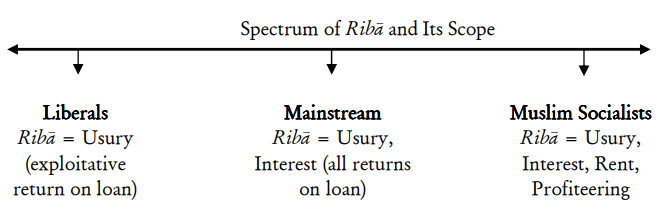
\includegraphics[width=0.9\textwidth]{CourantsIslamContemporain/ImagesCourantsIslamContemporain/Riba.png}

Rida part de l'analyse du mot \riba comme \textit{excès}, et en particulier reprend l'analyse de Co 3,125 présentée au début d'un excès lié à la renégociation de la dette. De là, il conclut que ce qui est interdit par le Coran sont les intérêts ajoutés à la fin de la période de prêt (\riba ’l-jahiliyyah). D'une certaine façon, ce sont les intérêts composés qui sont interdits, le fait que les intérêts augmentent en cas de non paiement. Cela lui permet d'autoriser les intérêts bancaires :
\begin{itemize}
    \item ils ne doublent pas les taux
    \item l'ajout d'un intérêt fait partie du principal de la même façon que le prix d'une vente à crédit (\emph{\riba al-buyu}) qui ne sépare pas principal et intérêt et qui est autorisé par le Coran.
\end{itemize}
 Il fait une distinction entre la \riba interdite dans le Coran et celle des Hadiths (voir graphique \ref{fig:MinorityRiba}) :

 \begin{figure}[h!]
     \centering
     \sidecaption{\cite{Siddique:DemystifyingRiba}, une séparation entre Coran et Hadith}
      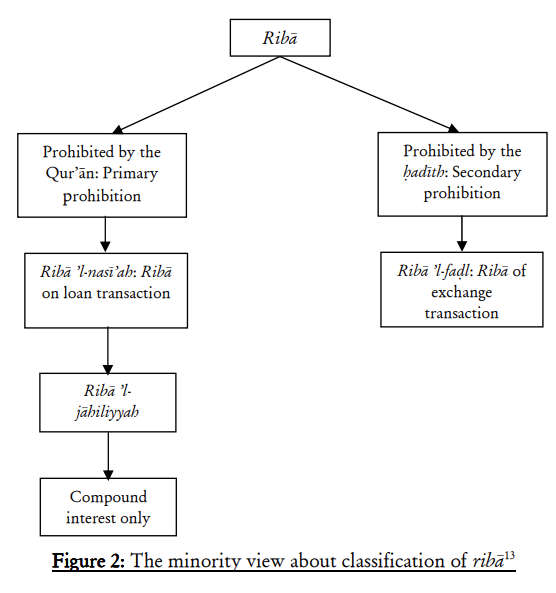
\includegraphics[width=0.5\textwidth]{CourantsIslamContemporain/ImagesCourantsIslamContemporain/RibaRida.png}
      \caption{La présentation du Riba selon Rida, dite minoritaire}
     \label{fig:MinorityRiba}
 \end{figure}
 
 Rida ne sera pas suivi par une majorités de jurisconsultes sur la légitimité des taux d'intérêt. En revanche, ils adopterons sa distinction entre less différents \riba, en étendant l'interdiction de la \riba du Coran à tout intérêt et pas seulement intérêt d'intérêt. Mais du coup, se pose la question du Hadith : pourquoi interdit-il  la \rib \emph{Al-Fadl}, c'est à dire la di
 
 

 
\paragraph{Les frères musulmans}
Dans les perspectives du réformisme musulman,
cette question d'ailleurs est loin d'être insoluble car une société qui émet des
actions peut être assimilée à une société en commandite. Les dividendes
représentent alors la part des bénéfices proportionnelle au capital engagé... 
al-Banna, fondateur des Frères Musulmans en Egypte, avait admis la licéité de ce
genre d'opérations et des Frères avaient, peu avant 1 948, fondé quelques ateliers
ou sociétés financées par ce procédé (2). La difficulté principale vient de ce que la
langue arabe n'a pas de mot spécial pour désigner les dividendes et que le terme
fâ'ida a des relents de ribâ.
\begin{quote}
    III. 2 interdiction de pratiquer l'usure, orienter les banques vers cette interdiction, le gouvernement doit donner l'exemple en abandonnant l'\textit{intérêt} fixé par les banque du prêt et du prêt industriel, etc. \textit{programme des frères Musulmans, 1936}
\end{quote}
%---------------------------------------------------------------------------------------------------------------
\section{Naissance de la finance et de l'assurance Islamique}

\subsection{Ce que l'on voit : Malaisie,...} 

\paragraph{une pratique supposant une \textit{shari'ah} qu'on ne peut interroger}

\subsection{Quelle est la théologie sous-jacente}

\paragraph{Une évolution de la shari'a par les principes} Mohammed Talbi 
\begin{quote}
    Il existe
trois principes en islam permettant de faire évoluer le droit et de
l'adapter
à la réalité, 

la \emph{maslaha} c'est-à-dire l'utilité publique, un
concept qui date du II\textsuperscript{e} siècle de l'hégire, 

la
\emph{zharoura}, la nécessité, c'est un principe fort puisqu'il est dit
que "la nécessité rend permis l'interdit" ; 

et les \emph{maqassid}, les
finalités de la loi. 

\begin{Synthesis}
On part des principes contre les principes. 
\end{Synthesis}
\sn{voir p. \pageref{TroisPrincipesEvolutionsShari}}
\end{quote}


\section{Conclusion}

\paragraph{une variété importante de vision mais toujours basée sur la sharia}

\paragraph{une réflexion sur la base de la Sharia'}
voir ce que Candiard dit de ce théologien qui dit de ne pas faire de Kalam mais du droit.

\paragraph{quel pourrait être les pistes de Kalam, quelques pistes de l'expérience occidentale ?}

\paragraph{St Thomas et l'usure : une réflexion autonome de la théologie}

\paragraph{extension du juste prix dans les risques : la dimension actuarielle}
\paragraph{Au XIXème, réflexion neo-thomiste et patristique pour sortir du carcan}
Après avoir regardé comment l'économie moderne, pensée au XVIIIème et XIXème questionne l'Islam à travers l'étude des différents courants de l'Islam contemporain, je poserai quelques pistes sur le propre questionnement du Christianisme. Après tout, le prêt à intérêt était aussi interdit au Moyen-äge en Europe. Ces pistes seront en particulier nourrie par l'étude de la pensée de Saint Thomas d'Aquin sur les taux d'intérêt et comment ces pistes peuvent nourrir la réflexion de la théologie musulmane. 

Nous catholiques au XIX par rapport à la modernité: renouveau thomiste et patristique. Liberté de pensée par rapport aux questions de l’époque
« A quoi on tient en vrai »
Le raccourci de certains théologiens musulmans : faire le court circuit pour repenser les choses : obsession juridique. Comment on sort du droit ? En faisant de la théologie. Et pour cela retour à la tradition
Voile
Le coran la dit donc il faut se voiler. Voile : hijab n’est pas dans le coran. Rideau
Zina : qu’il faut cacher
Jilbab pour les filles et femmes du prophète 
Ibn el jahouzi : voile non mentionné. Dimension non religieuse

Des écrits au XX. Deux raisons : les femmes vont occuper plus de rôle dans l’espace publique.
Et renouveau de l’anti théologie. Le voile est une question de théologie. Question de la foi
	⁃	Saint Paul : la foi et les œuvres
	⁃	On comprend croyant non pratiquant
	
\chapter{Matériaux bruts pour validation}

\section{A lire}
\href{https://www.persee.fr/doc/ridc_0035-3337\_1955\_num\_7\_3\_9521}{Le prêt à intérêt et l'usure au regard des législations antiques, de la morale catholique, du droit moderne et de la loi islamique }

\section{Refus de l'intérêt en milieu chrétien}

\subsection{1163 : le concile de Tours condamne le prêt à intérêt}


Le 01 septembre 2014

La condamnation du prêt à intérêt par l'Eglise n'a pas empêché, au travers de divers subterfuges, le développement du crédit, moteur de l'activité économique.

Dans l’Occident chrétien médiéval, le rôle de prêteur sur gages, souvent pour de faibles montants, sera longtemps assuré par des juifs, que leur religion autorise à prêter avec intérêt à des non-juifs. Mais dès le XIe siècle, de nombreux bourgeois chrétiens enrichis se livrent au prêt à une autre échelle. Déjà au XIIe siècle, des bourgeois d’Arras, de Cahors, des Lombards d’Asti, des Génois prospèrent par ces opérations.

Certes, l’Eglise et les princes qui se conforment à sa loi bannissent le prêt à intérêt en s’appuyant - entre autres - sur l’Evangile de Luc : "Prêtez-vous l’un à l’autre sans rien en attendre." En France, le concile de Tours de 1163 condamne une des formes du prêt à intérêt dans le cadre de la moralisation de l’Eglise : nul clerc (évêque, abbé) ne peut désormais prêter de l’argent et recevoir en gage un

\section{Extrait site internet}
\begin{quote}
En Islam, le Riba est interdit : il s’agit de l’un des plus grands péchés, qui tire son origine du Coran. Mais il est également l’un des plus banalisés. Le Riba, appelé « usure », désigne l’intérêt perçu sur de l’argent prêté. De nos jours, le Riba est partout présent dans le domaine financier, à savoir, dans les comptes d’épargne, dans les prêts à intérêts, dans les agios… Alors, qu’est-ce que le Riba exactement ? Pourquoi est-il interdit ? Comment financer vos projets sans Riba 
\paragraph{Définition du Riba}

Le Riba peut être défini par intérêt - usure. Si le terme « usure » est la traduction la plus fréquemment donnée à cette interdiction de l’intérêt usuraire, il est important de préciser que le mot Ribâ vient cependant du verbe rabâ \& arbâ qui signifie augmenter et faire accroître une chose à partir d’elle-même. 

Dans le contexte financier, il est donc interdit de réaliser des transactions financières basées sur du Riba. Or, lorsque vous possédez un compte courant conventionnel, l’argent qui y transite alimente un circuit basé essentiellement sur l’usure. En effet, dans ce contexte, la banque dispose de vos fonds afin de spéculer. Même principe lorsque vous êtes à découvert : les agios que vous devez payer vous impliquent dans la pratique de l’usure.

Mais ce n’est pas tout : lorsque vous épargnez votre argent sur des comptes de type livret Jeune, Livret A, ou PEL, les intérêts que vous touchez sont également basés sur la pratique du Riba, et cela que vous fassiez don ou non des intérêts.

Enfin, lorsque vous réalisez un prêt bancaire, vous participez au développement de l’usure en payant des intérêts. 

\paragraph{De nombreux versets du Coran interdisent la pratique de l’usure.}     En voici quelques-uns, qui sont particulièrement explicites :

Verset 130 de la Sourate 3, Al-Imran : « Ô les croyants ! Ne pratiquez pas l’usure en multipliant démesurément votre capital. »
Les versets 278 et 279 de la Sourate 2, Al-Baqarah : (V-278) « Ô les croyants, craignez Allah ; et renoncez au reliquat de l’intérêt usuraire, si vous êtes croyants. (V-279) Et si vous ne le faites pas, alors vous recevrez l’annonce d’une guerre de la part d’Allah et de son prophète. Et si vous vous repentez, vous aurez vos capitaux. Vous ne lèserez personne, et vous ne serez point lésés. »
D’après Abu Hurayra, le Prophète (SAWS) a dit : « Evitez les 7 turpitudes ». Lorsque les compagnons demandèrent : « Quelles sont-elles, Ô envoyé d’Allah ? », il mentionna l’usure aux côtés notamment du polythéisme, du meurtre…
D’après Sahih Muslim : Ubâdah Ibn As-Sâmit rapporte que le Messager d’Allah (SAWS) a dit : « Or pour Or, argent pour argent, blé pour blé, orge pour orge, datte pour datte, sel pour sel, de manière égale, de main en main. Si la nature des produits diffère, vendez comme vous le voulez, si c’est de main en main ». \sn{\href{https://firstunion.fr/quest-ce-que-le-riba/}{First Union} ? }
\end{quote}

 
 \paragraph{Abd ar-Rahman ibn Nasir as-Sadi}\href{https://fr.wikipedia.org/wiki/Abd_ar-Rahman_ibn_Nasir_as-Sadi}{Abd ar-Rahman ibn Nasir as-Sadi} Oulema Hanbalite saoudien 1889. influencé par 	
Ibn Taymiyya
Mohammed ibn Abdel Wahhab
 
 \paragraph{ Le ribâ (l’usure) dans l’Islam}
 
 \href{https://www.ajib.fr/le-riba-lusure-dans-lislam/}{Le riba est l'usure dans l'Islam}
 
 \begin{quote}
    


Pour comprendre le sens réel du ribâ, pour connaître son statut légal dans l’islâm, houkm, qui est bien sûr, l’interdiction, ainsi que les méfaits individuels et collectifs qu’il engendre, il faut comprendre quelques points importants.

Parcourons ensemble ces extraite du livre « Le résumé des vertus de la religion musulmane » du grand savant \textit{Abdarrahman As-Sacdî} qui nous éclaireront sur la vue de la législation islamique, \emph{shariah}, sur les transactions, licites et illicites, ainsi que la sagesse du Législateur, Allah, soubhânah, en établissant cette auguste législation.

Nous verrons en particulier, les problèmes qui concernent le ribâ.

\begin{quote}
    
Que signifie le ribâ ?

Le ribâ signifie l’usure. Si l’on entend par « usure » le prêt à taux supérieur à zéro.

Car la définition contemporaine de « l’usure » est « l’intérêt excessif » ou « l’intérêt supérieur au taux légal », tandis que le ribâ est le prêt à intérêt, aussi minime soit-il.

Le prêt islamique légal est donc le prêt à zéro intérêt. Et le ribâ est l’usure dont l’intérêt est supérieur à zéro.

Il y a plusieurs types de Ribâ :
\begin{itemize}
    \item 1/Le prêt à intérêt : le surplus, aussi minime soit-il, perçu, pour le prêt, par le créancier en échange du délai accordé.

 \item 2/Ribâ al-fadhl : le surplus perçu lors de l’échange d’un bien ribawî (relatif au ribâ) tel que l’échange de l’or avec l’or, de l’argent avec l’argent, du blé avec le blé… etc.

 \item 3/Ribâ an-nasî’ah : différer l’encaissement lors d’un échange d’un bien ribawî de même nature, tel que l’or avec l’or, ou de nature différente, mais dont la cause ribawique est commune, tel que l’or avec l’argent.
\end{itemize}


\paragraph{Quelles sont les transactions dites légales dans le \emph{shariah}, halal ?}

La vente rendue licite par la législation islamique ainsi que le louage[1], les sociétés et les différentes transactions ; celles où s’échangent les marchandises entre les gens, les dettes, les utilités… etc.

\paragraph{Pourquoi une transaction est légale dans le \emph{shariah}, dite : halal ?}

La législation parfaite a permis ce type de transaction et l’a autorisé aux hommes, car cela assure leurs intérêts – nécessaires, indispensables ou complémentaires -.

Elle a élargi ainsi considérablement la liberté des hommes afin que leurs affaires et leurs conditions se réforment et que leurs vies s’ordonnent.

Quelles sont les conditions de la légalité d’une transaction ?

\textbf{La législation, \emph{shariah}, posa comme conditions pour que les transactions soient licites :}

1-La satisfaction des deux parties ;

2-la clarté du contrat ;

3-la connaissance de l’objet du contrat, de la durée du contrat et des conditions qui en résultent.



Quelles sont les transactions interdites dans la \emph{shariah}, dites : haram ?

La législation, \emph{shariah}, a interdit tout ce qui comporte un préjudice ou une injustice tel que :

1-Les différents types de jeu de hasard,

2-le Ribâ ;

3- l’ignorance[2], la jahâlah.
\end{quote}
 

Cette division, licite et illicite, halal et haram, prescrite par Allah et révélée à Son Prophète Mouhammed, ainsi qu’à tous les Prophètes avant lui, a pour objectif essentiel de préserver le but premier escompté par ces opérations d’échange entre les humains : l’intérêt mutuel, l’avantage commun à toutes les parties de l’échange et le bénéfice pour tous.

Inversement, tout ce qui n’apporte pas d’intérêt commun et ne fait pas bénéficier toutes les parties qui opèrent la transaction est illicite, haram et interdit.

Car cela va à l’encontre de la raison de cette opération d’échange, la transaction, qui est l’intérêt commun et l’absence de préjudice.

\textbf{Le ribâ fait partie de cette catégorie car son intérêt va dans un sens unique, qui est celui de l’enrichissement du créancier, et il porte un préjudice considérable au débiteur.}

Ceci s’appelle : injustice, iniquité et celui qui en profite ne fait que manger l’argent et les biens des autres injustement.
 \end{quote}
 
 
 \paragraph{Dictionnaire du Qoran}
 

 \section{Demystifying Riba through the Methodology of Muslim Jurists}
 \href{https://www.proquest.com/docview/2352353188?accountid=143046&parentSessionId=Sg7rHgjzHS0M9aF4pv1Nx2pxOOyR5LkKvILKrOVqG1o\%3D&pq-origsite=summon}{Demystifying Riba through the Methodology of Muslim Jurists}\sn{MUHAMMAD ZAHID SIDDIQUE; MUHAMMAD MUSHTAQ AHMAD.
Islamic Studies; Islamabad Vol. 58, N° 2,  (Jun 30, 2019): 169.}
 \cite{Siddique:DemystifyingRiba}



 \subparagraph{Summary}
  \begin{quote}
  In the post-colonial world when Muslims tried to restructure their public life in accordance with the shari‘ah, they developed a new discipline known as Islamic economics one of the central constructs of which is prohibition of riba. Unfortunately, the discussion among modern academic circles assumed a wrong methodology, which resulted in mystification of this concept and, hence, in a number of unsettling questions. This paper explains the nature of the mistake committed by modern Muslim scholars and economists. It also outlines the structure of correct methodology, which was laid down by premodern Muslim jurists for understanding the concept of riba and all other legal terms. The paper develops a consistent analytical framework for addressing majority of the questions on the subject of riba and attempts to rectify the mystification created around this concept.
  
  \end{quote}
 \subparagraph{Texte intégral}
 \begin{quote}

Keywords: riba, interest, loan, bay‘, Islamic economics, Islamic legal theory, financial regulations of Islam.

1. Introduction

After losing their political rule to the imperial powers, Muslim societies faced the widespread dominance of interest-based banking system. According to the majority of Muslim scholars and jurists, bank interest (riba) was not allowed, but Muslim societies got engaged in it due to growing spread of interest-based banking in modern societies and the non-availability of interest-free banking. \mn{noter aussi que le développement de la banque s'est fait en parallèle dans les sociétés occidentale. }

Muslim scholars and economists demanded its alternative soon after Muslims got independence from their foreign masters. Commitment to follow religious teachings in the public affairs of life and liberty from the colonial oppressors provided the required room, which resulted in what is now known as Islamic economics in general and Islamic finance/banking in particular.

One of the central concepts of Islamic banking is prohibition of riba, which unfortunately and surprisingly remained controversial among Muslim economists and scholars. Different perspectives about the meaning of riba prevailed in the twentieth century. Majority view holds that both usury and bank interest are equally impermissible in Islam while business profit is allowed.\footnote{1 For  detailed  arguments  of  this  position,  see  Ab┴ ’l-A‘la  Maud┴di,  S┴d  (Lahore:  Islamic Publications,  2000),  110–12;  M.  Umer  Chapra,  “The  Nature  of  Riba  in  Islam,”  Hamdard Islamicus  7, no.  1 (1984):  3–24;  Muhammad  Shafi‘, Mas’alah-i  S┴d  (Karachi: Idarat  al-Ma‘arif, 1996), 43–47; Muhammad Ayub, “What  is Riba? A  Rejoinder” Journal of Islamic  Banking and Finance  13,  no.  1 (1996):  7–24;  Muhammad  Taqi Usmani,  The  Historic  Judgment  on Interest Delivered in the Supreme Court of Pakistan (Karachi: Idarat al-Ma‘arif, 1999), 12–16; Mohammad Nejatullah  Siddiqi,  Riba,  Bank  Interest  and  the  Rationale  of  Its  Prohibition  (Jeddah:  Islamic Research  and  Training  Institute, 2004),  45–48;  and  Mahmoud A.  El-Gamal,  Islamic  Finance: Law,  Economics,  and Practice  (Cambridge:  Cambridge University  Press, 2006),  46–52. Within this  category,  there  are  further  two  approaches.  One  approach  that  represents  traditional ‘ulama’ emphasises the resurgence  of only those business contracts that were approved by  the early  Muslim  jurists.  It proposes  profit-and-loss  sharing (PLS)  as an  ideal alternative  to riba. Though it does not deny the permissibility of other than PLS-based financing instruments such as murabahah and ijarah, yet it affirms that equity-based financing method is the primary means of achieving desirable economic objectives. The second approach is pragmatic one. It justifies a more liberal and flexible stance on structuring shari‘ah-compatible transaction forms that looks for financial engineering to meet all demands of modern banking customer.  }

Contrary to the majority view, some modern Muslim scholars dispute that the Qur'anic term riba includes interest paid and charged in the banking system.\footnote{ Muhammad Rashid Rida (d. 1935) was among the foremost proponents of this theory. See his al-Riba  wa ’l-Mu‘amalat  fi ’l-Islam  (Cairo: Dar  al-Manar, 2007).  Also see  Sayyid  Yaqub Shah, “Islam  and Productive  Credit,” The  Islamic  Review  47,  no.  3 (1959):  34–37; Fazlur  Rahman, “Riba  and  Interest,”  Islamic Studies  3, no.  1 (1964):  1–43; Timur  Kuran, “On  the Notion  of Economic  Justice  in  Contemporary  Islamic  Thought,”  International  Journal  of  Middle  East Studies  21,  no. 2 (1989): 171–91;  Izzud-Din Pal,  “Pakistan and  the Question  of Riba,”  Middle Eastern Studies 30, no. 1 (1994): 64–78; and ‘Abd al-Karim Athari, S┴d Kiya Hay? (Mandi Baha’ al-Din: Anjuman-i Isha‘at-i Islam, 2008), 8–12}
To them, replacing bank interest with anything else is tantamount to obstructing natural operation of economy and creating inefficiencies because interest is the just reward of capital reflecting its marginal productivity. \sn{ Constant  J.  Mews  and  Ibrahim  Abraham,  “Usury  and  Just  Compensation:  Religious  and Financial Ethics in Historical Perspective,” Journal of Business Ethics 72, no. 1 (2007): 1–15}

3 According to this perspective, there is no need to have anything distinct like “Islamic banking” to begin with because the existing system is already Islamic.


Finally, on the other extreme are \textit{Muslim socialists}\sn{A l'autre extrême ?} who develop their version of Islamic economics based on socialist policy package.\sn{See Ghul┐m A╒mad Parvaiz, Ni╘┐m-i Rub┴biyyat (Lahore: Id┐ra-i ║ul┴‘-i Isl┐m, 1978). }

 Since socialism considers wage as the only legitimate reward of a factor input, the scope of riba is much wider than usury and bank interest according to these scholars. 

It is believed by some\sn{Raf┘‘ All┐h Shih┐b, Kir┐yah-i Mak┐n┐t k┘ Shar‘┘ ╓aithiyyat (Lahore: Kit┐b Ghar, 1981)} that rental earnings on an asset is also included in riba because rent is similar to interest earnings as both are the prices of capital determined by similar market forces. Others are of the view that not only bank interest but also trade or merchant profit is banned under the category of riba.


6 They argue that as lender is forbidden the right to charge interest from poor borrower, so should be the rich industrialists and landlords from appropriating lion's share of value-added on the name of profits.

They assert that loaning riba (riba 'l-qard) covers money lenders and hoarders who charge against time while riba of excess (riba 'l-fadl) is the domain of landlords, merchants, and middlemen who exploit poor workers and make unequal exchanges. 

These differing perspectives are shown in figure 1. Because this last perspective about riba has gained very little popularity among Muslim scholars and masses as compared to the first two, we exclude its analysis from the scope of this paper, though it would be analysed indirectly.


Spectrum of Riba and Its Scope Liberals Mainstream Muslim Socialists Riba = Usury Riba = Usury, Riba = Usury, (exploitative Interest (all returns Interest, Rent, return on loan) on loan) Profiteering


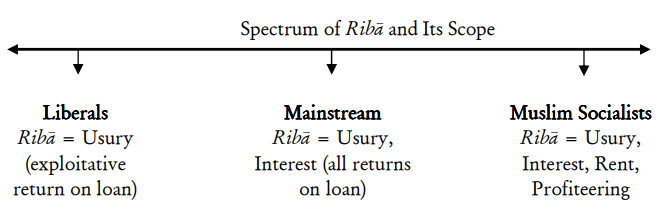
\includegraphics[width=\textwidth]{CourantsIslamContemporain/ImagesCourantsIslamContemporain/Riba.png}



The above differences have left scholars divided on several important questions that demand straightforward answers. Those questions include the following ones:
\begin{itemize}
    \item 
1. Is bank interest prohibited in the light of the Qur'an and the sunnah? If yes, how?
    \item 
2. Whether the Qur'anic term riba includes all kinds of interest rates or it relates only to the excessive interest rates?
    \item 
3. Whether the scope of riba extends to the interest charged and paid on business transactions in the banking system or is restricted to the interest charged on consumption loans only?
    \item 
4. Does Islam allow loan transactions? If yes, how and in what form?
    \item 
5. Is paying interest a lesser evil as compared to charging it?
    \item 
6. Is borrower always \textit{mazlum} (a losing party) in an interest bearing loan transaction?
    \item 
7. Does Islam allow indexation of loans on the grounds of inflation?
    \item 
8. Is credit-sale with higher deferred price as compared to the spot price allowed?
    \item 
9. Does Islam approve of “time value of money,” especially when charging higher deferred price is allowed in a credit sale?
    \item 
10. Are future currency contracts permissible in Islam?
    \item 
11. How and to what extent is salam transaction permissible?
\end{itemize}


These are but a few questions.
\begin{Synthesis}
We show in this paper that whatever confusion prevails among contemporary scholars on this subject is the outcome of following an inadequate methodology for determining the meaning and scope of riba.
\end{Synthesis}
 In fact, this methodology has mystified the nature of riba, which is otherwise clear when viewed from the methodological view point of the eminent Muslim jurists of the past. The mystification is such that not only it results in confusing answers to these questions but it also begets confusing questions. Unfortunately, the confusion has built up to the extent that the Federal Shariat Court of Pakistan has been struggling to come up with a definition of riba. It is in this background that this paper attempts to explain:

(1) the contemporary Islamic economists' methodology of interpreting and classifying riba; (2) why this methodology is wrong and insufficient; (3) the methodology of understanding riba on the pattern of Muslim jurists of the past; (4) that the methodology given by the Muslim jurists is coherent and compact.

The reader will encounter a number of arguments in this paper that are advanced by those who justify bank interest. Since the paper deals with the legal substance and not with the economic merits of arguments, hence we will restrict ourselves to the legal analysis of those arguments and leave aside their economic analysis and rationale, which require an altogether different methodology. Any legal system has three aspects: (1) what: the legal rulings (i.e., ahkam); (2) how: the rules of deriving those legal rulings (i.e., usul al-fiqh); and (3) why: the underlying rationale(s) and wisdom behind the legal rulings (i.e., hikmah)

It is important not to mix these aspects. The present study deals with the first two aspects of the issue of riba. Moreover, the classification of riba discussed in this paper is primarily based on the methodology of Hanafi jurists for ensuring analytical consistency. We presume that a school of law represents an internally coherent system of interpretation and that mixing up the views of the various schools results in inconsistencies.7 However, views of the other schools have been briefly mentioned in the footnotes wherever required. Finally, the paper does not attempt to show that the Hanafi jurists' approach is superior to all others, rather it explains that the classical jurists' approach (whether Hanafi, Maliki, Shafi‘i or Hanbali) to understanding riba is superior to that of the modern scholars. The methodology of these jurists share several common results that are important in order to answer the above questions.

Following section outlines the method adopted by modern Muslim scholars and economists. The next section discusses problems in this methodology and develops the skeleton for the methodology that is then applied in the coming section, which details out the general rules of riba alongside their resulting implications. The last section concludes the paper by giving a comprehensive definition of riba based on discussions in sections three and four.


\newpage
\subsection{Outline of the Mystifying Methodology}

Imran Ahsan Khan Nyazee\sn{\href{https://en.wikipedia.org/wiki/Imran_Ahsan_Khan_Nyazee}{Pakistan} Nyazee's academic career was inspired by the work of Abdur Rahim. Nyazee argues firstly, that due to its unique set of principles of interpretation, each school of Islamic law represents a theory of law unto itself. Secondly, he points out that Istiḥsān cannot be understood without understanding of the workings of qiyās. It is, therefore, difficult to accept that there was no system of interpretation before al-Shāfi‘ī's time. Thirdly, he concludes that the uṣūl al-fiqh never existed. Furthermore, Nyazee describes beyond the individual fikh of each school of law, another theory of interpretation called maqāṣid al-sharī‘ah (theory for the purpose of the sharī‘ah) which was developed by al-Ghazālī. Nyazee has written and self-published on a number of aspects of Islamic law. He agrees with most Muslim scholars that strictly speaking, selling money (taking interest) is prohibited, according to Islamic law. Some point out a difference between the treatment of riba in the Qur'an versus the Sunnah but Nyazee the two approaches are actually one and the same.Nyazee also proposes that all loans (except those of a charitable nature without a fixed period of repayment) and therefore all banking is prohibited and unIslamic. Nyazee is equally intolerant of murabaha, the Islamic system of business where in-put costs and mark-ups are made transparent between vendor and buyer. He argues riba will inevitably enter such transactions.[10] He extends the prohibition to the creation of wealth on the basis of debt and the fractional reserve banking system. These elements along with zakat (the system of alms-giving) he says, are the differences between Islam and capitalism. He advocates the use of the gold and silver dinars and dirhams as the currency of the Muslim community. Nyazee would also prohibit the corporation or 'legal personality' under Islamic law.} explains that the methodology adopted by modern scholars for determining the meaning of riba is the same, though they disagree in their conclusion regarding whether or not bank interest is riba.8 The fundamental problem of their methodology lies in overlooking the inherent link between the Qur'an and sunnah. This methodology of interpreting riba was initiated by Muhammad Rashid Rida (d. 1935) \sn{voir p. \pageref{Theol:Rida} Frère musulman pas le voyage en Europe. Plue el manar un commentaire coranique, sensé être l'héritage d'abdu}, which goes as follows:9

\paragraph{Lecture de Rida El Manar}
Riba is classified into two categories, riba of the Qur'an (also equated with riba 'l-nasi'ah, i.e., interest on loan transaction) and riba of hadith (equated with riba 'l-fadl, i.e., interest on exchange transaction).

Rida begins with literal meaning of the word riba (excess) and then traces some riba-based transactions practiced by Arabs during the time of Prophet (peace be on him). Rida, relying on some commentators of the Qur'an, asserts that the Qur'anic verse regarding riba deals with a specific practice of Arabs known as credit-sale where the payment of price is deferred to a future period while delivery of goods takes place on spot. Because a seller is allowed to charge whatever price he wants in a sale transaction, no riba is involved in the original price negotiated between the two parties-any excess in future price becomes part of the price. However, they used to increase the price excessively whenever the debtor would be unable to settle his debt obligations at the end of payment period. The debtor was given the option, “Will you pay the debt or increase the amount in lieu of delay?”

For Rida, it was this excessive rate (doubling and multiplying) of interest in debt-based transactions added to the original sum at the end of payment period which was prohibited by the Qur'an (he called it riba 'l-jahiliyyah).10 From this, he concluded that the bank interest is not the same riba that was deemed impermissible by the Qur'an because (a) it is neither doubling and redoubling of rates (b) nor the excess is stipulated in the initial period of the banking transaction-he assumes that the initially added interest is part of the principal or original sum just like the original sum in case of credit-sale. 
\begin{Synthesis}
Hence, for Rida, only compound interest is prohibited.
\end{Synthesis} 

Other scholars, supporting Rida's view, added that business loans were not common among Arabs as theirs was a subsistence economy; loans were largely taken by poor people for consumption purposes on interest and whenever they were unable to repay them at due time, excessive interests were added to the original sum. Hence, it was this type of interest that was declared prohibited by the Qur'an and it has nothing to do with the modern commercial loans, \textbf{which are mutually beneficial for both parties.}11

Having ascribed this meaning to the Qur'anic word riba on the basis of some historical traces, Rida then explains the form of riba declared impermissible in the sunnah as a distinct prohibition from that of the Qur'an.
\begin{Def}[Riba] Usure, profit ou gain réalisé sur un prêt.
\end{Def}

\begin{Def}
[Riba al-buyu] : Usure. Opération de vente dans laquelle une matière première est échangée contre la même matière première mais en quantité différente et la livraison d’une des matières premières est postposée. Pour éviter le riba al-buyu, les matières premières échangées par les deux parties devraient être en quantités égales et l’échange devrait être instantané. Riba al-buyua a été condamné par le Prophète Muhammad afin d’éviter que le riba (intérêt) n’affecte insidieusement l’économie.
\end{Def}
\begin{Def}[Riba al-duyun] : Usure d’une dette.
\end{Def}
 
\begin{Def}[Riba al-fadl] : La différence de quantité entre deux biens échangés et comportant du riba.
\end{Def}
\begin{Def}[Riba al-nasiah] : La différence de paiement liée au report de deux biens comportant du riba
\end{Def}\mn{cf Glossaire des termes financiers  Islamiques \href{https://www.cairn.info/la-banque-et-la-finance-islamiques--9782804167042.htm}{Banque et finance islamique} } He calls it \textit{riba 'l-fadl} which emerges in the exchange of two counter values of the same or different species and hence also called \textit{riba 'l-buyu‘}.12 The position of Rida, which may be termed as minority view, is summarised in figure 2.


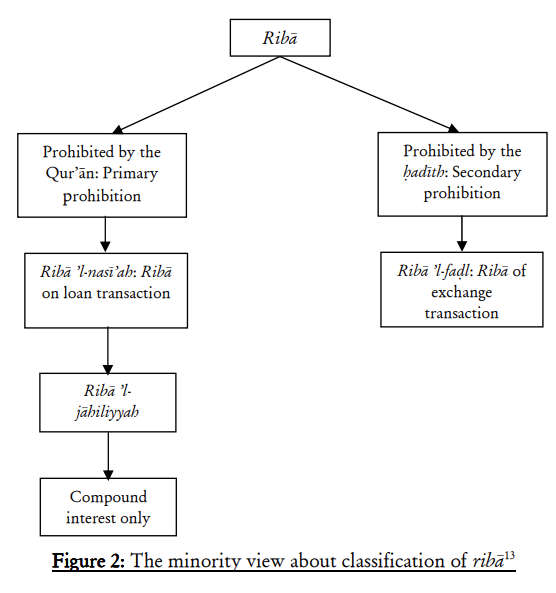
\includegraphics[width=\textwidth]{CourantsIslamContemporain/ImagesCourantsIslamContemporain/RibaRida.png}

Thus, Rida dichotomised the two concepts of riba, one attributed to the Qur'an and another to the sunnah. He finally declared the first one as real or explicit riba while latter as lighter or implicit riba.
\textbf{
Though the majority of contemporary scholars did not agree with the conclusion drawn by Rida about legitimacy of bank interest, however they adopted his methodology of classifying riba. The only difference in their opinion is that riba of the Qur'an includes all rates of return on loan and it is not merely restricted to the compound interest of jahiliyyah}\sn{la période pre islamique}


To them, business loans were a part of Arab's economy and any contractual return to lender is unfair because this is tantamount to refusing to share business risk with the borrower. We can depict their views in figure three.
\begin{Synthesis}
On a donc un nouveau problème, le pret commercial lié avec l'industrie et face à ce nouveau problème, une lecture de Rida qui est assez positive (Riba = Excess) mais qui note une différence entre Coran et Sunna) et fait une distinction entre les deux, reprises ensuite par les autres légistes, mais en repartant d'une lecture stricte du Riba comme intérêt. Il conveint d'articulier Coran et Sunna de façon non parallèle mais l'un par l'autre.
Il convient de montrer l'évolution du prêt commercial au XIX
\end{Synthesis}
Because the sunnah is not linked with the Qur'an in this methodology, both the minority and majority Muslim economists have struggled to explain as to why someone would engage in exchange transactions of the forms mentioned in hadith. Some opined that these transactions are declared impermissible because they may open the path for the “real riba” (i.e., riba of the Qur'an).


14 Others assumed that it was meant to discourage the practice of barter exchange and promote market exchange through a medium of exchange.15 Yet another view argues that it eliminates the possibility of benefiting from asymmetric information of the contracting parties.16 The truth is that none of these explanations makes the point.

2.1. The Nature of Debate within Minority and Majority Schools

The debate that has taken place within the followers of this mystifying methodology on the issue of why or why not bank interest is riba may briefly be summarised here. As explained above, Rida asserted that bank interest was not included in the Qur'anic concept of riba of debt because it was different from the riba that was charged by Arabs on credit-sale transaction by doubling and multiplying the price whenever the debtor was unable to settle his debt at due time and asked for relaxation in payment period.18 Rida explained that the Qur'anic verse “Allah has permitted bay‘ and prohibited riba”19 referred to this riba. To strengthen his case, he argued from the verse: “O Believers! Do not devour riba doubled and multiplied and fear God so that you may prosper.”20

This verse complements the former verse in the sense that what was implicit in the first verse was made explicit in the latter-both verses referred to the practice of doubling and multiplying of interest and none of them forbad the bank interest.

How do the majority of scholars respond to this argument? For example Usmani notes the Qur'anic verse:

O you believers! Fear God and give up riba that remains outstanding if you are true believers. Behold! If you do not obey this commandment, then God declares war against you from Himself and from His Prophet. But, if you repent (from riba), then you are entitled to only your principal amounts. Neither should you inflict harm to others, nor others should do harm to you.21

The argument is based on the emphasised words ‘you are entitled to only your principal amounts (ra's al-mal)'. He infers from these words that the rightful entitlement of lenders is the original sum advanced; he cannot charge any increase whether small or large (doubled and tripled). To him, the verse (3:130) forbids a severe form of riba where interest is multiplied, but it does not restrict riba to this specific form. Hence, bank interest falls within the purview of the Qur'anic verse “Allah has permitted bay‘ and prohibited riba.”22 They are also of the view that charging interest on commercial loans was also practiced by Arabs.23

Does the above analysis of mainstream scholars guarantee the prohibition of bank interest? We are afraid it does not. Their arguments rest on two assumptions:

(1) The verses (2:278-79) address the issue of loan-transaction.

(2) Ra's al-mal (principal amount) can only refer to the original principal advanced in loan.

Both of these assumptions are problematic. Following submissions can be made against them:

(a) If the meaning of the verse is to be determined with reference to historical practices, one can equally claim, just like Rida, that the verse is not about loan transaction but about credit sale. In that case, ra's al-mal is not referring to the principal amount lent; rather, it is the deferred future price of the goods sold. On which legal grounds or facts can this claim be dismissed?

(b) Further, this deferred price might include increase over and above spot price. Hence, the future price could consist of two components: spot price plus some additional profit. The sum of these two would constitute ra's al-mal (principal amount) in this transaction (i.e., principal amount in credit sale (ra's al-mal) = spot price + extra profit)

Whenever a debtor was unable to repay full amount, further multiplied increase was added to this original sum, Rida called it interest. This would increase the due amount to: total amount after increase added due to delay, which is interest in addition to ra's al-mal.

Using this structure, one can then argue that the initially added interest in a loan transaction is equivalent to initially added “extra profit,” which becomes part of ra's al-mal. Therefore, entitlement to the ra's al-mal means entitlement to the simple interest, as claimed by Rida.

(a) The only legal justification for ascertaining that the verse is about loan transaction is based on the words “ra's al-mal” (principal amount). But how can it be settled that ra's al-mal here means ra's al-mal of a loan transaction? This question is important because a number of transactions constitute a component of ra's al-mal. For example, there is ra's al-mal both in mudarabah and musharakah contracts. How to exclude these forms of ra's al-mal from the purview of the Qur'anic verse? If someone says, “This verse is about loan, so ra's al-mal refers to that of loan contract and not of mudarabah and musharakah,” he is clearly arguing in circularity. The argument goes like this:

Q: How do we know that the verse is about loan contract?

A: Because the verse talks about ra's al-mal.

Q: How do we know that ra's al-mal here refers to that of loan?

A: Because the verse is about loan contract!

A circular argument is no argument.

(b) Muslim Socialists could maintain that ra's al-mal means principal amount of all business contracts. Therefore, it is not legitimate to charge any excess over and above principal amount, no matter it is mudarabah, musharakah or ijarah.

Not only that the analysis of mainstream scholars does not necessarily imply the prohibition of bank interest, it leads to a set of unsettling arguments that have left Islamic economists bewildering about some basic issues. For example,

(1) Even if it is agreed that ra's al-mal means principal amount of a loan transaction, does it mean “nominal” amount or the “real” (inflation adjusted) amount? Again, what are the legal grounds to settle this issue? Because there are no clear-cut legal grounds available in this methodology, we see scholars are divided on this subject matter-some allow indexation of loan against inflations while others do not.

(2) What about the question of “time value of money?” This question poses challenge for Islamic economists because they, as a rule, approve the practice of charging higher price in credit-sale and murabahah.

(3) The Lawgiver has allowed salam, what are the legal grounds for not extending this permission to currency salam (future currency contracts)?

Undoubtedly, majority view has addressed these issues, but the answers do not seem to be stemming out of a coherent analytical legal system. This approach is often found mixing up legal analysis with economic analysis. This missing coherent analytical legal system is the root cause of most of the mystification that has prevailed all over. It is an unfortunate state of affairs and it is high time to demystify things.

3. Methodological Assumptions of Premodern Muslim Jurists (Fuqaha') for Understanding Riba

To understand the method used by the eminent premodern Muslim jurists for understanding riba, three methodological issues (MI) need to be clarified. They are explained by Nyazee in detail.24

1) Link between the Qur'an and Sunnah

The methodology adopted by the modern Muslim scholars and economists is misleading because it delinks the Qur'an and sunnah. It assumes that the meaning of riba is different in the Qur'an and sunnah, which is not the case. To explain the nature of error made by both the groups, it should be noted that Muslim jurists (fuqaha') classified riba in the category known as mujmal (unelaborated)25 whose meaning and scope cannot be determined without explanation (bayan) of the Lawgiver (Shari‘). The famous hadith (as given in footnote 1) that explains different usurious transactions actually does not add something to the Qur'anic word riba. Rather, it defines its meaning and scope.

Thus, while to the contemporary scholars the meaning of riba is known independent of hadith and they see hadith as adding some more cases to the Qur'anic concept of riba, the jurists say that hadith is the definition of the term riba used by the Qur'an. Thus, riba 'l-nasi'ah and riba 'l-fadl both are included in the Qur'anic concept of riba.

2) Relationship between Loan and Bay‘ (Exchange)

Loan is also classified as a form of exchange transaction (bay‘)26 by Muslim jurists. The scope of this paper does not allow detailed analysis of this assertion.27 For descriptive purposes, it can be seen that a loan of Rs X is an exchange of Rs X today with Rs X after time deferment (and with Rs X + Y if interest payment of Rs Y is included). Figure 4 depicts this nature of loan transaction by illustrating a loan transaction between Mr. A and B:

3) Skeleton of a Coherent Legal System

A coherent shari‘ah-based legal system consists of a set of general rules, called

‘azimah by the jurists, supplemented by some exemptions to these laws, called rukhsah. In the words of Nyazee, ‘Azimah (lit. determination, resolution) is applied to mean a rule that is applied initially and for itself. Such rules form the backbone of the law. As against this, there may be a rule that goes contrary to the requirements of the initial rule, but is permitted by the law. This rule is considered to be a rukhsah (exemption) from the initial rule.28

This classification of ‘azimah (the higher or first order rules) and rukhsah (the lower or second order rules) is important for several reasons.

First, it explains the order in which the rules have to be applied.

Second, it explains why sometimes two opposing cases may be allowed within a given skeleton of law.

Third, the order of rules implies that an exception cannot be extended using any method of argument, whether analytical or analogical. On the other hand, extension of first order rules is legitimate by these methods. In other words, it is not allowed to build a sub-legal system based on exemptions because otherwise it starts negating the primary provisions and objectives of the law-an exemption from the general rule must remain an exemption.

Fourth, because of the logical hierarchy in the operations of ‘azimah and rukhsah, it is clear that an exemption from a rule cannot be used to nullify or change the shari‘ah status (hukm) of any other case that is derived from the general rules. Alternatively put, an exemption (a lower order rule) cannot prevail over the higher order rules.

Fifth, because all rules and exemptions are derived from nusus (the Qur'an and sunnah), hence the only justifiable exemptions are the ones, which are given in nusus (i.e., stated by the Lawgiver Himself).

We call these nusus the “facts” of the shari‘ah-based legal system in this paper. Given these “legal facts,” the task of a jurist is to derive those general rules (‘azimah) from the facts, which render these facts internally consistent and extendible on the one hand and highlight the exemptions (rukhsah), if any, on the other.29 Finally, the general rules and exemptions generate some implications, called ahkam. This skeleton of a shari‘ah-based legal system is illustrated in Figure 5. We apply this skeleton in this paper to elaborate riba.

The relevant “legal facts” used by premodern Muslim jurists to derive general rules and exemptions are quoted at the relevant places in this article. We are now in a position to take on the issue of derivation of the general rules and the implications from those “facts.”

4. Underlying Rules behind the System of Bay‘ in Jurists' Methodology

Our intention in this paper is to reveal that the apparently large and complicated system of legal injunctions (ahkam) is reducible to a few set of rules derived from fewer legal facts. We propose that a majority of ahkam (legal injunctions or provisions) governing economic transactions (buyu‘) can be derived from three broad rules:

1. Rules of riba mentioned in the sunnah. This is not a single rule, rather a set of rules as explained below.

2. Rule about the sale of goods not possessed by a person.

3. Rule about exemption that an exemption is to be treated as exemption.

Before explaining these rules, we first explain the context of the Qur'anic verses that underlies the jurists' methodology of riba to clarify the misconception that the relevant verses of Surat al-Baqarah are about loan transaction and not exchange (bay‘).

4.1. The Context of the Verses of Surat al-Baqarah

The Qur'an states that the disbelievers said, “Verily, bay‘ (sale) is just like riba.” In response to this, it was said, “Allah has permitted bay‘ and prohibited riba.” To understand why the disbelievers said this, consider these three transactions:

(a) A gives B 100 grams of gold in exchange of 110 grams of gold to be paid after one year. This is primarily a sale contract as explained previously (i.e., exchange of 100 grams gold with 110 grams gold with time lag) and involves riba (how, this will be explained in the next section but take it for granted for the moment).

(b) A asks B for 100 grams of gold in exchange of, say, 500 kg wheat at spot. This is a legitimate regular sale contract.

(c) A demands from B 110 grams of gold in exchange of 500 kg wheat for payment of price after one year: this is credit sale contract with higher deferred price as compared to spot price and is also legitimate (this is explained in section 4.3).

The credit sale was a common practice among Arabs and, therefore, they were confused as to why the transaction (a) is impermissible and (c) is permissible while the two are quite similar in nature (i.e., both are credit sales and both involve access payment). In (a), 10 grams of additional gold are paid as counter-value for 100 grams of gold for a delay of one year and similarly 10 grams of gold are paid for a delay of one year in transaction (c). It is for this reason that disbelievers said, “Verily sale is just like riba!” That is, transaction (c) (i.e., the credit sale) is similar to the transaction (a). The technical reason for allowing transaction (c) and forbidding (a) is the similarity of genus which is explained by the sunnah. This is explained in the next sections in detail, but the important point to note here is that the assumption that the Qur'anic term riba is not about sale contract, rather it is about debt, is not implied by these verses.

Thus, the verse says that Allah has approved all forms of buyu‘ (exchange transactions) except those which involve riba.30 The natural question then arises: what is this thing called riba? Has the Qur'an given any definitive description of riba?

One may make one of the two assumptions here. First, the concept of riba was largely a sort of common knowledge for everyone and, hence, it required no legal description by the Qur'an. That common knowledge is traceable by an examination of historical record of Arabs which provides sufficient legal foundations for determining the meaning of riba. As far as the details of riba in the sunnah are concerned, they were additions over and above to that common knowledge of riba and most of these additions were unknown to the Arabs. The liberals and mainstream scholars share this assumption and we believe that this assumption constitutes what we called the “mystifying methodology.”

Second, some forms of riba may be or actually known to the Arabs but these do not set the legal standard against which the Qur'anic concept of riba is to be determined. As it is a legal term, its meaning has to be sought from the Lawgiver. In technical sense, the jurists call it mujmal (unelaborated) for which elaboration (bayan) is sought from the Lawgiver. This elaboration of the legal meaning of the Qur'anic term riba is given by the sunnah. After this elaboration by the Lawgiver, its meaning is determined definitively and it becomes mufassar (elaborated). This is the methodological assumption that the jurists use not only for defining riba but also for other legal terms of the Qur'an, such as salah, zakah, and so on.31 Thus, according to this second assumption, the practices and concepts of Arabs may be referred by the Qur'anic concept riba but it is not the benchmark against which we assign legal meaning to the Qur'anic terms.

For example, the Arabs had some concepts about how to offer salah (prayer), but this information does not define the legal meaning of the Qur'anic term salah nor is this concept limited to this information set. Similar is the case with riba. The Arabs might have been aware of some forms and practices of riba but that does not constitute the legal definition of riba. When the jurists classify a term as mujmal, they mean that this term is a technical legal term and its meaning should be determined with reference to the words of Lawgiver Himself, neither by the linguistics (dictionary) nor by the historically known social concepts and practices that hover around that technical term. It should be emphasised here that considering riba as mujmal does not mean that the Arabs did not know the meaning of this word at all. Nor does it mean that the pre-Islam Arabs did not identify certain transactions as riba-in fact they did and the jurists did consider it part of riba.32

It only means that the meaning of riba in Islamic law is not limited to, and is not based on its usage in the pre-Islam Arabia. The Qur'an and the sunnah added several shades of meaning to this concept. That is why, it became a “technical term” of Islamic law. Hence, its meaning and scope cannot be determined by its dictionary meaning or its practice and understanding by the pre-Islam Arabs. Rather, it must be determined by the Qur'an and the sunnah, like any other legal term such as salah and zakah. Just as we cannot classify concept salah as salah of the Qur'an and salah of hadith, similarly we cannot dichotomise riba. Once it is established that the meaning of riba must not be gathered from pre-Islamic usage and practices but from the Qur'an and the sunnah, the next question is: how to explain the various usages of riba in the Qur'an and the sunnah? The answer, as per the well-established methodology of the jurists, is to consider the sunnah as the elaboration of the mujmal verses of the Qur'an.

This methodology is employed by the jurists for determining the meaning and scope of salah and zakah as well as riba. Let's follow through the path of righteous ones here and have its blessings.

4.2. General Rules of Riba When Transacted Species are Same

Keeping these in mind, one has to understand the classification of riba in the system of Muslim jurists. Because the sunnah defines riba, note the words of hadith,

When you exchange gold for gold, silver for silver, wheat for wheat, rice for rice, dates for dates, and barely for barely, then exchange like for like (in equal measure) and exchange them hand to hand (at spot), else it will be riba.33

To understand what it says, consider these transactions:

1) exchange of 1 gram gold for 1 gram gold on spot;

2) exchange of 1 gram gold for 2 grams gold on spot;

3) exchange of 1 gram gold at spot for 1 gram gold with delay;

4) exchange of 1 gram gold at spot for 2 grams gold with delay.34

As per the hadith, the first transaction is allowed; the second one is disallowed because it involves excess in measurement/quantity (called riba 'l-fadl); the third transaction is also impermissible because the hadith says that the exchange of homogeneous goods is allowed in equal measurement provided it is on spot; therefore, this transaction involves the riba 'l-nasi'ah (i.e., riba of delaying); finally, the fourth transaction involves both types of riba. These transactions provide two guiding rules (R):

R 1.1) Goods of the same species cannot be exchanged immediately unless their measurement (in terms of weight or volume) is same.

R 1.2) Goods of the same species cannot be exchanged with time lag, even with same measurement.

4.2.1. Implications

Five important implications (I) should be noted.

I. 1) Impermissibility of Market for Loanable Funds

Application of rule 1.2 gives the important implication that loan, with or without interest, is prohibited in Islam because, as explained above, a loan is an exchange of homogeneous goods with time lag. Does it mean that loaning is not allowed in Islam under any circumstances? Of course, this implication of the general rule is at odd with a number of legal facts (nusus), which promise reward for offering loan to the needy ones. How to reconcile these apparently contradictory legal facts now? This is where the concept of rukhsah (exemption) is activated by the jurists. Though loaning is against the general rule (‘azimah) given by the Lawgiver, yet it is allowed by Him as an exemption from this prohibition if it takes the form of benevolent giving (tabarru‘ or sadaqah).35 Loan is classified as tabarru‘ if:

(a) it is out of the intention of benevolence to the other person (i.e., the lender consciously bestows upon the borrower the benefits associated with his asset);36

(b) no increase in its value is stipulated, else it would cease to be benevolent and would involve riba 'l-fadl; and

(c) no contractual time limit is stipulated, the lender can ask for his asset anytime he wants.37 Stipulating (legal) time constraint in loaning activity makes it a business transaction as per the application of general rules of shari‘ah and, hence, unlawful because in that case it is simply the exchange of homogeneous goods with time delay, which is not allowed, whether or not interest factor is included. Moreover, making the time period binding would imply that the lender is forced to do, or to continue with, an act of charity. This is against the very nature of charity.

In short, this principle implies that Islamic law does not permit the “market for loanable funds.” It sees loaning as an act of benevolence, especially in favour of one's relatives.38 Stated alternatively, loan is purely a social transaction (a means of tying and strengthening social bonds) in Islam and not a business. It was in this social transaction capacity that the institution of loan prevailed for thousands of centuries not only in Muslim societies but also in other civilisations of the world until the emergence of capitalism in the fifteenth century.39 Note that this important result (impermissibility of the market for loanable funds) does not follow directly from the classification of modern scholars of Islamic economics, as the majority view allows interest-free non-benevolent loans as a general rule and not as an exemption.

This implication answers one of the important arguments in favour of bank interest given by some economists. The argument says that interest should be allowed in shari‘ah because interest is the price of capital and without interest the market for loanable funds cannot be equilibrated. Because we are not dealing with the economic merit of arguments in this paper, we ignore its economic substance and comment on its legal merit only. It is clear from the above implication now that this argument has no shari‘ah basis because shari‘ah does not allow market for loanable funds to begin with, let alone equilibrating it from shari‘ah perspective.

Before moving on to the next implication, the important implication and exemption regarding loan transactions be noted:

I 1.1) A loan transaction is prohibited, whether or not interest factor is added to it.

I 1.2) A benevolent interest-free loan is recommended as an exemption to the general rules of riba by the Lawgiver.

I. 2) Impermissibility of Bank Interest

All forms of bank interest, whether simple or compound, are prohibited by Islam as per Rules 1.1 and 1.2. Similarly, the fact whether loan is made for business or consumption purposes makes no difference to this result. There remains no confusion about these conclusions if the shari‘ah rules are applied with consistency. In fact, the practice of charging interest by the bank includes both kinds of riba and it, therefore, may be stated that it is the most comprehensive form of riba! This can be verified from the figure 6, which depicts detailed structure of riba-based transactions in case of homogenous goods (leaves aside heterogeneous goods for the moment).

I. 3) False Dichotomy between “Giving and Taking” Riba

The recipient of riba is not always the lending party as is usually perceived. It can be seen from above examples that in case of transaction (2) the lender is the beneficiary of riba, but in transaction (3) riba is received by the borrower, and finally both are its recipients in transaction (4). Hence, opinions such as “taking riba is a greater evil than giving it and, hence, paying interest to the bank is a lesser evil” are based on the fallacious assumption that it is only the bank that receives interest in a typical interest-bearing loan transaction. This wrong assumption is the outcome of using the wrong methodology outlined in section two.40

I. 4) Mutually Beneficial Riba is Prohibited

The view that bank interest realised in transaction (4) is or should be permitted (as claimed by liberal Muslim scholars) is implicitly based on the assumption that “two wrongs make one right”-that is, it assumes that mutually enjoyed riba of the lender and borrower can make this transaction acceptable while the matter of fact is that each of them is separately prohibited to begin with.

I. 5) Irrelevance of Time Value of Money

Following the wrong methodology has resulted in another confusing argument that the bank interest should be allowed because of “time value of money.” This argument is based on the presumption that Rs. 1 today is worthier than Rs. 1 tomorrow. Why? Economists believe that this is due to the subjective time preferences of an individual. A rational (i.e., self-interested utility maximising) economic agent is said to have positive time preferences in the sense that consumption today is preferred to consumption tomorrow because the latter is uncertain, which makes him impatient, thus he wants to have it today than tomorrow.

Another reason for having this positive time preference emerges from the institutional arrangements: if I have the option of earning some interest (say Rs. Y) on Rs. 1 by putting it in a bank account today, why should I lend it to someone for free? Putting Rs. 1 in a bank account will make it “Rs. 1 + Rs. Y” for sure (assuming away bank insolvency), say, after one year while lending it to someone will leave it worth Rs. 1. Hence, Rs. Y (which may be expressed in percentage) is the price that should be paid to the lender for a loan of one year, else it would be unfair with him. This argument is more of economic than legal in its substance, however, some comments can be made here to evaluate its legal substance in the light of preceding discussion.

The relevant part of the proposed argument is the second one (the institutional arrangement) because the first one is merely a subjective feeling, which may differ from person to person (as a matter of fact, not everyone prefers to consume more today than tomorrow). The argument presumes that there exists and should exist a well-established legally functional market for loan, which coordinates interest-based loan transactions. But just recall “I.1” that Islam does not approve of the market for loan to begin with. Eliminate this institution of market for loan, and the argument disappears. The point is that the concept of “time value of money” conceived in this economic sense is alien to the discussion of riba. Its validity presumes that there exists a legal institutional market for loanable funds where money is growing continually and, therefore, an individual always has the option of putting his money in that market.

Not only that this assumption is invalid from the point of general rules of shari‘ah as explained, it is also in contradiction with the ontological structure of the universe and economic facts.

The above is not the only format of this argument, it is phrased in some other shades as well. For example, it is stated that money could buy benefits and had the lender not lent it he could have benefitted himself. This implies that lending is an act of sacrificing the benefits associated with money. Therefore, the lender should be compensated for this sacrifice and interest payment is exactly that reward. This reward makes sense given that the borrower takes benefit out of money. The argument is valid to the point that money is beneficial to the lender and that if he makes the choice of not lending it, he can benefit from it. Moreover, it is also true that the borrower enjoys the benefits associated with the money. None of these facts is denied by the shari‘ah rules. But these facts alone cannot formulate the required case for this argument; it requires a moral statement in its premise to derive the desired conclusion.

To see this, note that the argument does not end here, after quoting these facts it then makes a moral assertion: “it is morally (and hence legally) right if money is lent for reciprocal benefits.” Addition of this moral statement is necessary for validating the conclusion that “interest is the just reward for lending.” But this moral assumption contradicts the general rules of the shari‘ah, which are laid down above. Seeking reciprocity in loan is exactly what that changes its status from tabarru‘ to loan as a business transaction and, hence, it becomes nothing but riba. The argument here is quite straightforward:

The owner of money is granted the right of benefitting from his money by shari‘ah rules; he is given the option of making a conscious choice of transferring the benefits associated with his money to another person as an exception to the general rules by the shari‘ah, but there is neither any general rule nor any exemption from the Lawgiver that assigns him the right of lending money in the name of the so-called “mutual benefits” (refer to I. 4 above). Legally speaking, this involves both riba 'l-fadl (because the homogeneous goods are exchanged at different rates) and riba 'l-nasi'ah (because time stipulation is invoked-the lender asks for the excess of measurement for parting with the benefits of his money for a specified time).

Another variant of this argument comes with the heading of “effects of inflation on money.” We deal with it in the next section.

4.3. General Rules of Riba when Transacted Species are Different

What about the exchange of heterogeneous goods? The last words of the hadith are as follows: “If these species differ, then exchange as you like as long as it is from hands to hand.”

They give an immediate rule:

R 1.3) Goods of the different species can be exchanged with difference in measurement.

This rule says that such goods can be exchanged at different rates as far as measurement is concerned. In other words, riba 'l-fadl does not apply in case of heterogeneous goods. Is riba 'l-nasi'ah (prohibition of time delay in payment) also not applicable in this case? Apparently, it seems that it is not because of the words of hadith, “exchange should be on spot.” This has an odd implication that credit sale (sale of goods against money where payment is deferred to future time period) is not permissible under the shari‘ah rules. This is so because credit-sale is an exchange of heterogeneous goods with time lag. But the legal facts reveal that the Lawgiver has allowed credit-sale.41 How to explain this? Is credit sale also an exemption to the general rule, like a loan transaction? The answer is: “No, it falls within the general rules.”

To see how credit-sale is permissible within general rules, one needs to dig deep into the issue of the underlying cause (‘illah) that the Muslim jurists derived from the sunnah to understand the system of riba. The relevant question facing jurists was: Is prohibition of riba restricted only to the six goods named in the hadith or is it extendible to other goods? The answer of the jurists is, yes, it is extendible and for this extension they derived the underlying cause due to which riba was declared prohibited by the Lawgiver. Keeping aside the technical details and arguments, it should be noted that some of the goods are measured in terms of weight while others are measured in terms of volume. In the hadith under discussion, gold and silver were weighable while the other four items were volumeable at the time of Prophet (peace be on him).42 Based on this classification, the jurists derived two further rules:

R 1.4) when species are different but their method of estimation is the same (such as gold vs silver or wheat vs rice), unequal quantities can be exchanged, provided that the exchange is immediate;

R 1.5) when species are different and their method of estimation is also different (such as gold vs wheat), unequal quantities can be exchanged with time delay.43

Thus, the credit sale is allowed due to the application of Rule 1.5. To see this, consider these combinations of transactions:

1) Exchange of 1 gram gold at spot for 2 gram silver on spot (method of estimation same)

2) Exchange of 1 gram gold at spot for 2 gram silver in future (method of estimation same)

3) Exchange of 2 kg wheat at spot for 1 gram gold/silver on spot (method of estimation different)

4) Exchange of 2 kg wheat at spot for 1 gram gold/silver in future (method of estimation different)

The first transaction is allowed but the second is not because when species are measured by same method (i.e., “weight” in this case), then difference in the measurement (fadl) is allowed but deferment (nasi'ah) is not permissible. The third and the fourth transactions are allowed because here not only the transacted species are different but also their method of measurement (one was measured in “weight” while the other in “volume”).

In short, when both of the similarity factors (i.e., species and method of measurement) are found, then both fadl (excess of measurement) as well as nasi'ah (excess of time delay or time deferment) are prohibited. When similarity of measurement is found alone, then fadl is allowed but nasi'ah is prohibited. Finally, when none is found, both fadl and nasi'ah are allowed. Figure 7 depicts all of these rules completely (discussion about the last layer of boxes on the right-hand side of this figure is coming next).

The preceding discussion shows that the hadith explaining the nature of riba was not about the actual practices of Arabs that begged some economic explanations with which Muslim scholars have been struggling. Rather, it stipulated the rules of exchange. It says, “If at all you make exchange transactions, here are the governing rules.” Thus, all transactions that correspond to these general rules are allowed while those in contradiction with them are prohibited (however, some are exempted by the Lawgiver).

4.3.1. Implications

Following implications are derived from the above rules. It is important to note that the first two transactions mentioned in sub-section 4.2 belong to the case when method of estimation of the heterogeneous goods is same while the latter two cover the cases when their method of estimation is different.

I. 6) Placement of Regular and Credit-Sale

Transaction (3) is categorised as regular sale transaction (usually termed bay‘) by the jurists. On the other hand, transaction (4) covers credit sale, which may take two forms: with or without extra profit margin as compared to the spot sale. Because both measurement as well as payment time differential are allowed in this case, hence credit sale of both forms is allowed.

I. 7) Placement of Currency Exchange

The remaining two boxes are relating to the exchange of currencies (termed as bay‘ al-sarf by the jurists). A detailed description of these requires an appreciation of some more technical classifications44 made by the Muslim jurists. However, they are beyond the scope of this paper. Suffice to say that the jurists divided all tradeable species into two: (a) currency items, which are used as means of exchange; they included gold and silver (though other goods may also be treated as currency in this system) and (b) non-currency items, (goods that are exchanged, and are not medium of exchange). They roughly included all but gold and silver.45 Given this division, the jurists broadly mention four types of transactions (buyu‘):

(1) Non-currency item in exchange of non-currency item-called barter exchange.

(2) Spot or delayed currency (say gold) in exchange of spot non-currency (say wheat) item.

(a) If both of them (gold and wheat) are exchanged on spot, it is called regular sale of goods, and

(b) if the currency price (gold) is delayed, this is called credit sale.

(3) Delayed non-currency item (say rice) in exchange of spot currency item (say gold). Here, the price of the good is paid on spot while its delivery is delayed. This is called bay‘ al-salam (advance payment) by the jurists.

(4) One currency (gold) in exchange of another currency (silver)-known as bay‘ al-sarf.

Rules regarding the first two have been discussed above. Here, we have to make some submissions regarding this fourth type of transaction. Because this transaction comes under the umbrella of “different species with same method of measurement,” it is clear from figure 7 that the excess of measurement is allowed in this transaction while time deferment is not. This gives two further rules under rule (1.4):

1.4a) If different currency items (such as gold and silver) are exchanged, then it is allowed to exchange them at any rate;

1.4b) if different currency items (such as gold and silver) are exchanged, then it is not allowed to exchange them with time deferment.

If it is accepted that modern currencies are just substitutes of gold and silver, then two further important results emerge from this discussion:

I 7.1) Future Currency Contracts are Prohibited

Rules (1.4a) and (1.4b) imply that the spot currency transactions are allowed while their future contracts (known as currency salam in Islamic finance literature) are prohibited in Islam as they come under the purview of riba 'l-nasi'ah.

I 7.2) Indexing of Loans is Prohibited

Indexing the value of the currency loans against some underlying assets (say gold) on the ground of inflationary pressures is not allowed. It is often argued that since the value of currency decreases over time due to the presence of inflation, hence an extra-payment equal to the rate of inflation, over and above the original sum given in loan, should be allowed in favour of the lender to keep his purchasing power. Again, because the economic merit of this argument is beyond the scope of discussion in this paper, we restrict only to its legal merit. If it is accepted that one rupee is legally nothing but equivalent of 1 unit of gold or silver (whatever that unit be), then Rules 1.1 and 1.2 (governing the loaning contract in gold or silver currencies) should automatically become operational.

Those rules imply that (a) loaning in the form of currency item is allowed if and only if equal measurement (whatever the unit of measurement) is returned; else it would be riba 'l-fadl; and (b) it is a loan made out of benevolence and not business intention (having time stipulation); else it would be riba 'l-nasi'ah. Hence, adding an extra amount to loan transaction in the name of “indexation” is but both, riba 'l-fadl (because of the excess of measurement) and riba 'l-nasi'ah (because the increase is time bound). 46 Again, let simplicity and sanity prevail.

I. 8) Placement of Salam

To see how the jurists accommodated salam in this scheme, note that there is nothing in the set of rules 1 (from 1.1. to 1.5) which forbids it. However, according to rule 2 (given at the start of this section), selling what one does not possess is not permissible and this is exactly what a salam transaction involves. Thus, a salam transaction should not be allowed as per the general rules of shari‘ah. We are once again faced with the same issue: salam is permitted in the “legal facts;” how and where to place it in the legal skeleton of the shari‘ah? Is there another general rule, which governs its permission as we saw in case of credit sale or is it an exemption from the general rule just like loan? The jurists' answer is the following: Salam is permitted as rukhsah-exemption from the general rules-by the Lawgiver.47

Because it is an exception, as per rule 3, it would be allowed only as “one of its kind” (sui generis) and cannot be used as justificatory mode for deriving more comparable transaction forms (e.g., currency salam). An exception to the general rule remains exception and does not turn into a rule for other cases because then it ceases to be an exception and creates a situation of self-contradictory general rules, which is not acceptable in any legal system. Thus, salam transaction is allowed as an exception for those transactions where (a) a currency item is exchanged against a non-currency item and (b) non-currency item is deferred while the currency-item has been paid at spot.48 This is what the exception is all about; one cannot extend this exception to the transaction types where currency items are exchanged with each other because that would violate condition (a) of the exception case.49

Figure 8 shows a map of interplay among legal facts (nusus), general rules, exemptions, and the derived implications related to riba and bay‘ that are discussed in this paper. This diagram shows that a rather complex looking system of ahkam (implications) showing up at the ending layer boxes of figure 8 emerge out of a set of general rules, which are derived to make underlying legal facts compatible with each other.

5. Conclusion: The Definition of Riba

We conclude this paper by elaborating a comprehensive definition of riba that can be inferred from the discussions in this paper. Let's quote it from al-Sarakhsi:50
\begin{Synthesis}
Riba in its literal meaning is excess... and in the technical sense (in the shari‘ah), riba is the stipulated excess without a counter-value in bay‘ (sale).51
\end{Synthesis}


Let's explain it noting several points about this definition:

(1) Muslim jurists do not introduce the word loan in the definition of riba because they categorise loan transaction under exchange (bay‘). Not appreciating this point resulted in the misconception that since the fiqh conception of riba does not deal with the subject of bank loans, it needs to be inferred directly from the Qur'an.

(2) Riba is excess, either in the form of quantity (qadr) or in the form of benefits of delay (nasa'). The first is called riba 'l-fadl while the latter is called riba 'l-nasi'ah.

(3) This excess is without any counter-value permitted by the shari‘ah. Thus, the excess of quantity paid in lieu of time delay in case of interest-bearing loan is not allowed because these two cannot be the legitimate counter-values (see I. 4).52 For a substance to be counted as counter-value, it must be recognised by the general rules of the shari‘ah to begin with.53

(4) The excess is stipulated in exchange. If the excess is granted voluntarily, it would not be riba.

We started off with specific questions in the introduction. The appendix lists down the answers to these questions in the light of the above definition of riba. It can be seen that once the discussion about riba is placed on the right track, right and clear cut answers start emerging automatically.

Appendix: Questions and their Answers that Follow from the above Analysis

Notes

1 For detailed arguments of this position, see Abu 'l-A‘la Maududi, Sud (Lahore: Islamic Publications, 2000), 110-12; M. Umer Chapra, “The Nature of Riba in Islam,” Hamdard Islamicus 7, no. 1 (1984): 3-24; Muhammad Shafi‘, Mas'alah-i Sud (Karachi: Idarat al-Ma‘arif, 1996), 43-47; Muhammad Ayub, “What is Riba? A Rejoinder” Journal of Islamic Banking and Finance 13, no. 1 (1996): 7-24; Muhammad Taqi Usmani, The Historic Judgment on Interest Delivered in the Supreme Court of Pakistan (Karachi: Idarat al-Ma‘arif, 1999), 12-16; Mohammad Nejatullah Siddiqi, Riba, Bank Interest and the Rationale of Its Prohibition (Jeddah: Islamic Research and Training Institute, 2004), 45-48; and Mahmoud A. El-Gamal, Islamic Finance: Law, Economics, and Practice (Cambridge: Cambridge University Press, 2006), 46-52. Within this category, there are further two approaches.

One approach that represents traditional ‘ulama' emphasises the resurgence of only those business contracts that were approved by the early Muslim jurists. It proposes profit-and-loss sharing (PLS) as an ideal alternative to riba. Though it does not deny the permissibility of other than PLS-based financing instruments such as murabahah and ijarah, yet it affirms that equity-based financing method is the primary means of achieving desirable economic objectives. The second approach is pragmatic one. It justifies a more liberal and flexible stance on structuring shari‘ah-compatible transaction forms that looks for financial engineering to meet all demands of modern banking customer.

2 Muhammad Rashid Rida (d. 1935) was among the foremost proponents of this theory. See his al-Riba wa 'l-Mu‘amalat fi 'l-Islam (Cairo: Dar al-Manar, 2007). Also see Sayyid Yaqub Shah, “Islam and Productive Credit,” The Islamic Review 47, no. 3 (1959): 34-37; Fazlur Rahman, “Riba and Interest,” Islamic Studies 3, no. 1 (1964): 1-43; Timur Kuran, “On the Notion of Economic Justice in Contemporary Islamic Thought,” International Journal of Middle East Studies 21, no. 2 (1989): 171-91; Izzud-Din Pal, “Pakistan and the Question of Riba,” Middle Eastern Studies 30, no. 1 (1994): 64-78; and ‘Abd al-Karim Athari, Sud Kiya Hay? (Mandi Baha' al-Din: Anjuman-i Isha‘at-i Islam, 2008), 8-12 3 Constant J. Mews and Ibrahim Abraham, “Usury and Just Compensation: Religious and Financial Ethics in Historical Perspective,” Journal of Business Ethics 72, no. 1 (2007): 1-15.

4 See Ghulam Ahmad Parvaiz, Nizam-i Rububiyyat (Lahore: Idara-i Tulu‘-i Islam, 1978).

5 Rafi‘ Allah Shihab, Kirayah-i Makanat ki Shar‘i Haithiyyat (Lahore: Kitab Ghar, 1981).

6 Ziaul Haque, “The Nature and Significance of the Midieval and Modern Interpretations of Riba,” The Pakistan Development Review 32, no. 4 (1993): 933-46.

7 For details, see Imran Ahsan Khan Nyazee, Theories of Islamic Law: The Methodology of Ijtihad (Islamabad: Islamic Research Institute, 1994), 9-12.

8 Nyazee, The Concept of Riba and Islamic Banking (Islamabad: Institute of Advanced Legal Studies, 1995), 11-19. Imran Ahsan Khan Nyazee (b. 1945) is a well-known scholar and a prolific writer on the subject of Islamic law and is a former Professor of law in International Islamic University, Islamabad. His major works include Theories of Islamic Law; Islamic Jurisprudence; Islamic Law of Business Organization; and The Concept of Riba and Islamic Banking. He also translated some of the classical texts on Islamic law and jurisprudence, including: Hidayah of Marghinani; Bidayat al-Mujtahid of Ibn Rushd; Amwal of Abu ‘Ubayd; and first two volumes of Muwafaqat of Shatibi.

9 Rida, al-Riba wa 'l-Mu‘amalat fi 'l-Islam, 69ff.

10 Period before the advent of the Prophet (peace be on him) is referred to as jahiliyyah (i.e., the period of uncivilised state of affairs).

11 Fazlur Rahman, “Riba and Interest,” 7-8.

12 In this regard, a hadith reads, “The Prophet said, ‘While exchanging gold for gold, silver for silver, wheat for wheat, barley for barley, dates for dates, and salt for salt, exchange like for like, in equal measure, and exchange from hand to hand. If these species differ, then sell as you like as long as it is from hand to hand.'” Muslim b. al-Hajjaj, Sahih, Kitab al-musaqah, Bab al-sarf wa bay‘ al-dhahab bi 'l-wariq naqdan.

13 Adopted from Nyazee, Concept of Riba.

14 Maududi, Sud, 118-19.

15 Chapra, “Nature of Riba in Islam,” 3.

16 Siddiqi, Riba, Bank Interest and the Rationale of Its Prohibition, 49-50.

17 Adopted from Nyazee, Concept of Riba.

18 Rida, al-Riba wa 'l-Mu‘amalat fi 'l-Islam, 69-70.

19 Qur'an 2:275.

20 Ibid., 3:130.

21 Ibid., 2:278-79.

22 Ibid., 2:275.

23 For details, see Shafi‘, Mas'alah-i Sud, 106-120 and Siddiqi, Riba, Bank Interest and the Rationale of Its Prohibition, 38-40.

24 Nyazee, Concept of Riba, 35-36.

25 Mujmal is a term used by Muslim jurists to refer to a Qur'anic term that begs its explanation through the words of Lawgiver (i.e., God and His Prophet [peace be on him]). One cannot interpret mujmal either by looking its meaning in the dictionary nor can its meaning be determined through historical practices at the time of revelation of the Qur'an. Mujmal can be elaborated only by the Lawgiver. Another example of mujmal is the Qur'anic term salah (prayer) which cannot be interpreted literally.

26 Bay‘ means exchange of counter values, and is not restricted to sale of goods/services. Abu Bakr b. Mas‘ud al-Kasani (d. 587/1191), the illustrious Hanafi jurist, defines bay‘ as “exchange of property with property” and then elaborates that the concept includes not only ordinary sale but also barter, exchange of currencies, advance payment and many other forms of exchange. Bada'i‘ al-Sana'i‘ fi Tartib al-Shara'i‘, ed. ‘Ali al-Mu‘awwad and ‘Adil ‘Abd al-Mawjud (Beirut: Dar al-Kutub al-‘Ilmiyyah, 1997), 6:532-33. Abu 'l-Hasan ‘Ali b. Abi Bakr al-Marghinani (d. 593/1197), author of the authoritative Hanafi manual al-Hidayah, also explicitly asserts that qard (loan) begins as an act of charity but becomes an exchange transaction in the end. al-Hidayah fi Sharh Bidayat al-Mubtadi (Beirut: Dar Ihya' al-Turath al-‘Arabi, n.d.), 3:60

27 See Nyazee, Concept of Riba, 45-46.

28 Ibid., 49.

29 The Hanafis use the methodology of istihsan (juristic preference) for ensuring harmony and analytical consistency within the law when general rules and legal facts seem to contradict. If something appears prohibited in the light of the general principles of law, but has been explicitly permitted by one of the texts (i.e., legal facts), the Hanafi jurists take the position that it is permissible as an exception to the general principle. They use the rule, “prohibited under qiyas but permissible under istihsan” for this purpose. Exceptions to the general principles are made on the basis of the text, consensus, necessity or some other “covered principle” (qiyas khafi), which needs to be uncovered. Muhammad b. Abi Sahl al-Sarakhsi is worth quoting here: “This [istihsan] is the evidence coming in conflict with that apparent principle (qiyas zahiri), which comes into view without one's having looked deep into the matter.

Upon a closer inspection of the rule and the resembling principles, it becomes clear that the evidence that is conflicting with this apparent principle is stronger and it is obligatory to follow it. The one who chooses the stronger of the two evidences cannot be said to be following his own personal caprices.” Muhammad b. Abi Sahl al-Sarakhsi, Tamhid al-Fusul fi 'l-Usul, ed. Abu 'l-Wafa' al-Afghani (Beirut: Dar al-Kutub al-‘Ilmiyyah, 1993), 2:200-202. Another important point made by al-Sarakhsi is that when the jurist uses istihsan and prefers the stronger rule, he abandons the weaker one and as such it is not permissible for him or his followers to follow the latter. He goes on explaining that when istihsan is carried out on the basis of a concealed or covered principle (qiyas khafi), the established rule does not amount to be an exception but becomes a general principle in itself.

Interestingly, not only the Hanafi jurists but also the Maliki jurists explicitly employ the principle of istihsan for resolving the apparent anomaly found in the legal facts where one set of nusus prohibits a loan transaction and another set of nusus allows it. They hold that it is prohibited as an exchange transaction but allowed as an act of charity.

30 Al-Sarakhsi interprets this verse as the following: “Trade is of two kinds: permitted (halal), which is called bay‘ in the law; and prohibited (haram), which is called riba. Both are types of trade. Allah informs us, through the denial of the disbelievers, about the rational difference between sale (bay‘) and riba, and says, ‘That is because they said, “Sale is like riba.”' He, then, distinguishes between prohibition and permission by saying, ‘And Allah has permitted sale and prohibited riba.' Through this, we came to know that each one of these is trade, but only one form is permitted.” Al-Sarakhsi, al-Mabsut, ed. Hasan Isma‘il al-Shafi‘i (Beirut: Dar al-Kutub al-‘Ilmiyyah, 1997), 12:1-2.

31 The famous Hanafi jurist Abu Bakr al-Jassas al-Razi (d. 370/980) says, “In the law (shari‘ah), it (riba) is applied to meanings in which it was not used in the language. This is indicated by the fact that the Prophet (peace be on him) termed nasa' as riba in the tradition of Usamah b. Zayd (God be pleased with him). He said, ‘Verily, riba is in nasi'ah.' ‘Umar b. al-Khattab, (God be pleased with him) said that riba had different forms and out of these salam in teeth, that is, in animals, is not concealed. ‘Umar also said that the verse of riba was one of the last to be revealed, and the Prophet (peace be on him) was taken away before he could elaborate the details for us. Therefore, give up riba and the suspicion of riba. It is established from this that riba became a technical term, for had it been governed by its original meaning in the language, it would not have been obscure for ‘Umar, who was fully aware of the names used in the language, being a native speaker.

This (the conversion of the word into a technical meaning) is also indicated by the fact that the Arabs were not aware of the sale of gold for gold and silver for silver with a delay (nasa') as riba, but this is riba in the technical meaning. If this (meaning of riba) is as we have explained it, then, it became like all the other unelaborated (mujmal) words that are in need of an elaboration (bayan). These are terms that have been transferred from the language to the law and assigned meanings to which the word was not originally applied in the language, like salah, sawm, and zakah. Such words are in need of a bayan and it is not proper to employ them in legal reasoning for the prohibition of any of the contracts, unless an evidence has been adduced to show that such a meaning is employed by the law.

The Prophet (peace be on him) elaborated on many occasions the intention of Allah in a verse, by way of an explicit statement or in response to a query (tawqif), and through these he has indicated the evidence (dalil). The (legal) meanings are, therefore, not lost to those who have knowledge when they employ legal reasoning.... In the technical sense, the word riba is assigned several meanings. The first is the one that was prevalent among the people of the jahiliyyah. The second is excess in the same species out of things measured and weighed, according to the view expressed by our (Hanafi) jurists.... The third is nasa' (delay), which is of several types.” Ahmad b. ‘Ali al-Razi al-Jassas, ed. Muhammad al-Sadiq al-Qamhawi, Ahkam al Qur'an (Beirut: Dar Ihya' al-Turath al-‘Arabi, 1992), 2:183-84. Al-Sarakhsi is also worth quoting here:

“Mujmal is the word the meaning of which is not understandable except by asking the one who used this word.... An example of mujmal is the saying of the Almighty: “He prohibited riba” as riba literally means excess but we know that this is not meant here because sale has been permitted for the purpose of excess. Rather, riba here means prohibition of a sale due to an excess without a counter-value stipulated in the contract; and this excess is either in the form of increase in measure or by way of delay.... It is obvious that this elaboration is not known by literal analysis. Rather, it needs a separate source. Hence, it is mujmal with respect to its intended meaning. The same is the case of salah and zakah. They are also mujmal because their original literal meaning is prayer and growth, but because of their use in specific legal acts, their intended meaning cannot be gathered from their literal analysis.” al-Sarakhsi, Tamhid al-Fusul fi 'l-Usul, 1:168-69.

32 See al-Jassas, Ahkam al-Qur'an, 2:183-84.

33 Muslim, Sahih, Kitab al-buyu‘, Bab bay‘ al-ta‘am bi Mithlih.

34 One can simply substitute “Rs.” for “gram gold” in these transactions if Rs. (currency) is treated as substitute of gold and silver currency.

35 The famous Hanafi manual Hidayah explains the position of a loan transaction in the following words: “It is an act of charity in the beginning and that is why it is not valid from a person who does not have the capacity to do charity, such as a minor or a guardian (of a minor). However, at the end, it becomes a contract of exchange because it turns into exchange of dirhams with dirhams with delay, and that is riba.” See al-Marghinani, 3:60. The commentators explain, “This necessitates invalidity of loan but the shari‘ah has recommended it and the whole ummah agrees on its validity; hence, we hold that it is valid but not binding (and can be terminated at will by any party).” Akmal al-Din Muhammad b. Mahmud al-Babarti, al-‘Inayah sharh ‘ala al-hidayah (Bulaq: al-Matba‘ah al-Kubra al-Amiriyyah, 1316 AH), 5:273. The same position is upheld by Maliki jurists.

Thus, the famous Andalusian Maliki jurist Abu Ishaq al-Shatibi (d. 790/1388) says, “There are many examples of istihsan in the law, such as loan, which is riba in reality because it is exchange of dirham with dirham with delay; but it has been permitted because it benefits and facilitates the needy.” Ibrahim b. Musa al-Shatibi, al-Muwafaqat fi Usul al-Shari‘ah, ed. Abu ‘Ubaydah Mashhur b. Hasan (al-Khobar: Dar Ibn ‘Affan, 1997), 5:194-95.

36 Jurists apply the rules of ‘ariyah (commodate-loan) on these transactions because it is the nearest match for qard and the only way to legally justify a qard transaction. Al-Kasani, 10:600.

37 In much the same way as time period cannot be stipulated in a contract of ‘ariyah because no one can be compelled to do or continue with an act of charity (tabarru‘). Al-Marghinani, al-Hidayah, 3:60. In other words, making the condition of time-period binding changes the nature of the transaction and it no longer remains tabarru‘.

38 This has some income distributional as well as social consequences.

39 For an analysis of the idea of “debt as a social construct” and the transformation of this social construct to the impersonal market form, see David Graeber, Debt: The First 5,000 Years (New York, NY: Melville House Publishing, 2011, 308-60.

40 This false dichotomy is also not consistent with a number of “legal facts” (nusus). For example, in a hadith the Prophet (peace be on him), after explaining the rule of exchange among six goods, said, “Whosoever paid more or demanded more, indulged in riba.” Muslim, Sahih, Kitab al-musaqa, Bab al-sarf wa bay‘ al-dhahab bi 'l-wariq naqdan. Both are treated equally because both are the participants of “market for loan” which is not allowed.

41 The validity of credit-sale is inferred from many facts. These include the general permissibility of sale transactions such as the words of the Exalted, “Allah has permitted sale” (2:275). The jurists hold that all sales are permitted except those which have been prohibited specifically, such as sales involving uncertainty (gharar) or which stand prohibited by the operation of other principles of law, such as the prohibition of riba. The analysis in text explains that credit sale does not fall under the prohibition of riba.

42 This is the Hanafi position. The other schools classify these six items in different ways, but interestingly all classify them into two categories. The below table summarises their positions:

School Position on Gold and Silver Position on other Four Items Hanafi weighable (mawzunat) volumeable (makilt) Hanbali weighable (mawzunat) volumeable (makilt) and countable (ma'dudt) Shfi'i currency (thaman) edibles (mat'umat) Maliki currency (thaman) storable edible items (mat'umat)

The net result is that all the four schools agree on the applicability of the rules of riba on gold and silver (though for different reasons) and they come up with the impermissibility of loan transaction. For the Hanafis, they are also applicable on all items that are either weighed or volumeable (whether they are food items or not, does not matter); the Hanbalis agree with the Hanafis but add a third category of the counted items; for the Shafi‘is, the rules of riba are applicable on food items (whether they are weighed, measured or counted does not matter); the Malikis agree with the Shafi‘is but add a proviso that these food items must be such that people generally prefer to store them. These differences have interesting implications for extending the rules of riba to cases other than the six items specifically mentioned in the traditions. For details, see Nyazee, Concept of Riba, 83-88.

43 Interestingly, although the four schools have determined different ‘illah (cause) for the operation of riba on gold and silver, yet a loan transaction even if interest-free remains prohibited for all the four schools. Thus, for the Hanafis and the Hanbalis gold and silver must be exchanged on spot because they are weighable items, the Malikis and the Shafi‘is deem it necessary because gold and silver are currency items. Resultantly, despite disagreement on the ‘illah of riba, all the four schools agree that a loan transaction is prohibited as an exchange transaction and permitted only as an act of charity.

44 These include the terms ‘ayn, dayn, and thaman. For an elaboration of the meaning of ‘ayn and dayn, see Nyazee, Concept of Riba, 54-57.

45 The jurists treat gold and silver as thaman (price/currency) in exchange with all other items. Even when they are exchanged with each other (as in the contract of sarf), both of them are treated as thaman. That is why they are called thaman mutlaq (absolute thaman). Fungible items (mithliyyat) are deemed thaman if they are exchanged with non-fungible items (qimiyyat). When a fungible item is exchanged with another fungible item, such as when wheat is exchanged with barley, the parties are at liberty to consider any one of them as thaman but they have to specify it in the contract. For details, see al-Kasani, Bada'i‘ al-Sana'i‘, 7:216-17.

46 The last two implications are based on the widely accepted assumption that modern currencies are just like gold and silver currencies and should be treated as their substitutes. See Ghulam Rasul Sa‘idi, Sharh Sahih Muslim (Lahore: Farid Book Stall, 1998), 4:350-361; and Muhammad Taqi Usmani, Islam aur Jadid Ma‘ishat-o Tijarat (Karachi: Ma‘arif-i Islami, 1999). Changing this assumption can change the implications. The alternative to this view is to accept that modern money is a promise of payment, which implies that it is an acknowledgement of debt. In that case, Islamic rules of hawalah (endorsement) transaction will be applicable. Accepting this position can allow the indexation of loans since money is now treaded as value of something which it promises and, therefore, a loan can be linked to the underlying promised asset.

However, accepting the premise that “modern money is debt” leads to the result that exchange of currencies is not allowed even on spot because of another general rule of the shari‘ah, namely, “prohibition of exchanging debt for debt” (bay‘ al-kali' bi 'l-kali'). The prohibition is reported in by many scholars of hadith. For instance, see ‘Ali b. ‘Umar al-Daraqutni, Sunan, Kitab al-buyu‘, Bab nahy ‘an bay‘ al-kali' bi 'l-kali'; Muhammad b. ‘Abd Allah al-Hakim, al-Mustadrak ‘ala 'l-Sahihayn, Kitab al-buyu‘, Bab nahy ‘an bay‘ al-kali' bi 'l-kali'. Thus, one cannot maintain both of these positions simultaneously; either he has to allow indexation of loans or he has to allow exchange of currencies. For details, see Nyazee, Concept of Riba, 96-114.

47 The jurists cite traditions of various Companions who report that the Prophet (peace be on him) prohibited them from selling what they did not possess but gave exemption for salam. Al-Kasani, Bada'i‘ al-Sana'i‘, 7:101-02.

48 Some other conditions are also applicable for the validity of this transaction but they do not relate to our subject matter here. For their details, see al-Kasani, Bada'i‘ al-Sana'i‘, 7:103ff.

49 A misconception prevails regarding the nature of riba due to a tradition, “there is no riba except in nasi'ah (deferred payment transactions).” These words of Ibn ‘Abbas constitute reason that can explain the adoption of wrong methodology by the contemporary Muslim scholars. It is inferred from this tradition that the primary form of riba deals with loan transaction, which is riba 'l-Qur'an. However, several points invalidate this inference as indicated by al-Sarakhsi. See al-Sarakhsi, al-Mabsut, 12:11-12. First, the words of the hadith are quoted from Ibn ‘Abbas who initially had this opinion but he reverted from this position later on when the hadith of riba was brought to his knowledge by Abu Sa‘id al-Khudri. Second, the ahadith of riba are quoted by several Companions of the Prophet (peace be on him) through several sources. Therefore, they cannot be ignored out rightly in favour of this isolated narration.

Third, hence, it is necessary to place these words of Ibn ‘Abbas appropriately within the legal structure of the shari‘ah. Thus, al-Sarakhsi points that the words relate to the exchange of heterogeneous goods measured similarly, because in that case there is no riba except in deferment.

50 Apçna²'

51 Al-Sarakhsi, al-Mabsut, 12:109.

52 That is why, the definition of riba in al-Durr al-Mukhtar, a later Hanafi text, is given as follows: “Riba is an excess without any counter-value recognised by shari‘ah, in favour of one of the parties in a transaction.” Muhammad Amin b. ‘Abidin, Radd al-Muhtar ‘ala 'l-Durr al-Mukhtar Sharh Tanwir al-Absar, ed. ‘Adil Ahmad ‘Abd al-Mawjud and ‘Ali Muhammad Mu‘awwad (Riyadh: Dar ‘Alam al-Kutub, 2003), 7:398-401.

53 For example, if a female sells her body in exchange of mangoes, this would not be legitimate. Nor will it be legitimate if A lends Rs 1,000 to B on the condition that B will repay Rs 1,000 plus a swine.

Appendix: Questions and their Answers that Follow from the above Analysis No Questions Answers 1 Is bank interest prohibited in the light Yes, it is prohibited, because it is of the Qur'n and the sunnah? violation of rules 1.1 and 1.2. 2 Whether the Qur'nic term rib It includes all forms of interests. includes all kinds of interest rates or it This is a necessary implication of relates only to the excessive interest rules 1.1 and 1.2. rates? 3 Whether the scope of rib extends to It extends to all kinds of loans, the interest charged and paid on commercial or consumption, as business transactions in the banking shown by the application of rules 1.1 system or it is restricted to the interest and 1.2. charged on consumption loans only? 4 Does Islam allow loan transactions? If Loan is against the general rules of yes, how and in what form? Islam. However, it is permitted by the Lawgiver as an exemption to the rule if it takes the form of tabarru'. 5 Is paying interest a lesser evil as No, it is not. The assumed compared to charging interest? dichotomy is wrong, as it has been clarified by I.3. 6 Is borrower always malm (a losing No, the borrower can also be the party) in an interest-bearing loan receiver of rib as per rules 1.1 and transaction? 1.2 (see I.3). 7 Does Islam allow indexation of loans No, it does not. The demand for on the grounds of inflation? loan indexation is invalidated by rules 1.4a and 1.4b. 8 Is credit sale with higher deferred price Yes, it is validated by the application as compared to the spot price allowed? of rules 1.4 and 1.5. 9 Does Islam approve of "time value of No, it does not. In fact, the concept money," especially when charging is alien to the subject matter of rib, higher deferred price is allowed in a provided both the concept of time credit sale? value of money and rules of rib are used appropriately. 10 Are future currency contracts No, they are not. It is violation of permissible in Islam? rule 1.4b. 11 How and to what extent is salam Rule 2 implies that salam is against transaction permissible? the general rules of the shar'ah but allowed as an exemption by the Lawgiver, hence, should remain exemption as per rule 3.
 \end{quote}
 
 
 \paragraph{Chapitre 8. Islam et assurances}
 LES CAPITAUX DE L’ISLAM  | Gilbert Beaugé
 \href{https://books.openedition.org/editionscnrs/871?lang=fr}{ Islam et assurances}
\begin{quote}
    
L’assurance est-elle légale du point de vue de la Shari’a ? Ce débat aujourd’hui encore est très vif dans les pays musulmans\sn{1 En fait, quatre éléments ont permis de classer les contrats d’assurance parmi les contrats interdits par le clergé islamique : a) l’imprécision (gharar), b) le jeu de hasard (gimar), c) l’usure (riba) et d) l’échange de choses équivalentes (bai al sain bil-dain). Le travail le plus complet à ce sujet est celui de Muhammad Baltagi, Uqud al-ta’ min wigha al-figh al islami Koweit, 1982. K. Krüger donne une bonne vue d’ensemble du droit privé des États régis par le droit égyptien. Certains problèmes comme celui du riba sont analysés de façon plus détaillée, cf. Recht van de islam, 1987.}. La fonction sociale de l’assurance est tout particulièrement perçue par la population musulmane, dans la mesure où les catégories classiques du droit musulman intègrent cette valeur. Cette fonction suppose l’utilisation du principe d’assurance et, même dans un pays aussi conservateur que l’Arabie Saoudite, on ne rencontre aucune réserve à l’encontre de l’assurance sociale\sn{2 Introduit par décret royal, pp. 98 sv., n° 746 du 5.09.1969.}. En revanche, on continue à y critiquer l’assurance privée et, de temps à autre, cette critique réapparaît dans d’autres pays islamiques.

 
2 L’assurance peut se définir comme les précautions terrestres que l’on prend à l’encontre des coups du destin et des pertes matérielles, autant d’épreuves envoyées par Allah comme le sait tout musulman pieux. De ce point de vue, l’assurance peut apparaître comme le renoncement à la croyance en une prédestination, l’abandon de l’espérance en une miséricorde ou, pour le moins, comme leur limitation. A ces problèmes de nature religieuse ou morale qui, dans des périodes difficiles, comportent également un élément politique, s’ajoute, pour le musulman, la difficulté à concevoir la notion de risque et à la démarquer de celles de jeu ou de pari, afin de pouvoir en saisir la signification fonctionnelle, en rupture avec les contrats spéculatifs qu’interdit la Shari’a\sn{3 Cf. à ce sujet Al Amin Al Darir, Al Gharar wa-athauhu fil-uqud fil figh al islami.}. La discussion sur ce thème, qui se fonde sur des textes classiques de la Shari’a remontant au Moyen Age, s’est développée à la suite de l’implantation des compagnies d’assurance européennes dans l’empire ottoman, au cours de la deuxième moitié du xixe siècle, et des tentatives d’innovation des réformateurs de l’Islam, au début de ce siècle. Une opposition de type nationaliste et pan-islamique se manifesta alors à l’encontre de ces institutions capitalistes et occidentales, qui jouera un rôle non négligeable.
 
\subparagraph{HISTORIQUE DE LA NOTION D’ASSURANCE DANS LES PAYS DU MONDE ARABE}

3 La première réflexion approfondie sur la légalité de l’assurance en pays islamique tint compte de façon singulière des exigences musulmanes. Dans son ouvrage Radd al Muhttar, Ibn Abidin, représentant de l’école officielle de droit Hanafi dans l’empire ottoman, suggère en effet le compromis suivant : il serait licite d’établir des contrats d’assurance portant sur les risques encourus à l’intérieur du royaume islamique – le Dar al Islam – à condition que ces contrats soient conclus avec une compagnie d’assurance ayant son siège hors des pays de l’Islam, dans le pays des infidèles. La prise en charge du risque devrait se faire au siège de la compagnie\sn{4 Cf. l’étude complète de C.A. Nallino, « Belle assicurazioni in diritto musulmano banafita », in Oriente moderne, vol. VII, Rome, 1947. pp. 446 sv.}.

4 On estimait ainsi satisfaire suffisamment les besoins pratiques en assurances nécessités par le trafic international des marchandises, à une époque où Constantinople, Beyrouth et Alexandrie, ports par où transitait le coton, étaient les centres essentiels du commerce britannique du Levant, alors que le commerce français était davantage orienté vers les côtes d’Afrique du Nord.
 
5 Ce n’est que relativement tard, vers 1890, bien après la fondation de banques ou la création de filiales bancaires (1850), que fut créée une compagnie d’assurance à Alexandrie5. L’initiative en fut prise par trois Libanais qui reprirent la filiale d’une petite société anglaise s’occupant d’une affaire d’assurance-vie en Égypte, pour l’étendre, à partir de Beyrouth, à l’ensemble de la Syrie. Au début du siècle, au moment même où des sociétés françaises tentaient de s’établir en Afrique du Nord6, d’autres sociétés anglaises et françaises suivirent le mouvement, en Égypte puis dans les pays du Levant, tandis que la péninsulte arabique demeurait pratiquement à l’écart jusqu’au lendemain de la Seconde Guerre mondiale.

6 Le marché était peu porteur et étroit. Il s’agissait d’opérations d’assurance-vie, d’assurance-incendie et d’assurance-transport pour quelques biens importants. Ces assurances étaient souscrites par des banques étrangères ayant un intérêt particulier à le faire : par exemple, la Banque Ottomane travailla avec Eagle Star dans le domaine du crédit et de l’assurance hypothécaire. En raison de l’inflation qui suivit la Première Guerre mondiale, les polices d’assurance-vie perdirent leur valeur et il fut difficile de remplir de nouveaux portefeuilles dans un pays ruiné par la guerre. Les compagnies d’assurance ainsi que les courtiers s’orientèrent dès lors vers l’assurance des dommages et des transports à court terme. L’activité de ces entreprises était plus importante dans les pays sous influence britannique comme l’Égypte, le Soudan, la Palestine et l’Iran, alors que l’influence française dominait en Afrique de Nord ainsi que dans les pays du nord Levant, Syrie et Liban.


7 Si l’on prend l’exemple de l’Égypte, on constate qu’un système national d’assurance se mit en place, après la Première Guerre mondiale, avec la participation de trusts européens. Son évolution fut lente car le marché était étroit7 et il était nécessaire de former un personnel local. Le Conseil de surveillance introduit en 1939 maintint dans les limites du raisonnable une évolution qui, entre temps, s’était renforcée. Les pays sous influence française connurent également ce processus, sur les détails duquel nous reviendrons. Pour la Lybie, le marché italien eut une influence déterminante sur le système de l’assurance. Il connut une évolution moins marquée, mais parallèle.

 
8 La notion d’assurance privée s’imposa timidement comme instrument de la vie économique moderne dans les pays musulmans arabes. Les réserves de nature religieuse ne disparurent que progressivement : dans le secteur bancaire tout comme dans le secteur de l’assurance, les modernistes cherchèrent d’abord à obtenir des compromis. Ils tentèrent de prouver que les institutions et les pratiques que générait la vie moderne étaient compatibles avec les règlements de la doctrine islamique, mais ne tinrent pas suffisamment compte des réalités politiques et économiques8. Curieusement, le système d’assurance sociale, alors faiblement développé, fut tenu à l’écart de cette discussion. Il était, et reste toujours appréhendé, moins comme une assurance que comme une aide de l’État. Par ailleurs, jusqu’au tout début de la motorisation, les bases manquaient pour que soit mis en place un important volume d’affaires, aussi bien dans le domaine de l’assurance des personnes que dans celui de l’assurance des dommages. Dans les décennies qui suivirent la Seconde Guerre mondiale, les défenseurs du patrimoine islamique national s’opposèrent aux partisans d’une économie occidentalisée dirigée, ou tout au moins influencée, par des pays occidentaux. Sans se situer au cœur des débats, le système d’assurance fut tout de même soumis à examen critique : l’enjeu était d’établir s’il était ou non compatible avec les prescriptions de la Shari’a.
 
9 Ces discussions se développèrent à la fin des années cinquante, stimulées par un mouvement de création de compagnies nationales d’assurance et culminèrent lors d’une semaine de discussions à Damas\sn{Une telle manifestation avait eu lieu à Paris en 1951. Un des principaux orateurs, le professeur syrien Mustapha Ahmed al Zarga, démontra la compatibilité totale de l’assurance sous toutes ses formes avec la Shari’a, tandis que le professeur égyptien Abu Zahra n’envisageait que des associations mutualistes. L’ensemble des références figure dans un rapport complet de Zahra paru à Damas en 1962 : Aqd at-ta’min wa-mauqifal-shari’a al-islamiyya minhu.} : d’éminents juristes prirent position sur la question de l’assurance et l’on s’interrogea également sur la notion de risque et la manière de le définir et de le préciser dans un contexte économique. Le droit islamique, vers lequel il s’agissait de jeter des ponts, n’offrait sur ce terrain que peu de possibilités. Il fut très difficile, entre autre, de vaincre l’opposition unanime à tous les contrats sur les risques, assimilés aux jeux et aux paris\textsuperscript{10}. L’idée moderne d’une communauté organisée pour faire face à son destin\textsuperscript{11} – dont les bateaux et caravanes pouvaient fournir un exemple – et au sein de laquelle chacun participe de manière appropriée à la réparation des dommages, ne figure pas dans le droit islamique. 

\newpage
Sous cette forme, l’idée de risque demeure étrangère et incertaine\sn{ Le terme général est gharar, l’incertitude. \begin{Def}[gharar]
Gharar al-uqud signifie contrat à risque. Ils ont un rôle dogmatique. On range aussi sous cette dénomination les contrats portant sur des prestations que l’on peut préciser, mais qui ne l’ont pas été lors de la signature.\end{Def} Cf. art. « gharar », ainsi que le commentaire de l’article 484f « äegyptisches Zivilgesetzbuch von Sanhuri » (cf. supra, note 14). voir \href{https://fr.wikipedia.org/wiki/Abd_el-Razz\%C3\%A2q_el-Sanhour\%C3\%AE}{Sanhouri et code civil Egyptien}} au musulman, qui aimerait voir codifier non seulement ses devoirs religieux, mais également ses relations vis-à-vis du monde qui l’entoure. La seule chose sensiblement comparable à une assurance personnelle est le financement d’une rente à vie, sorte de rente viagère (umra) prélevée sur les bénéfices retirés de la terre ou de tout autre bien. Toutefois, une telle institution a suscité de nombreuses réserves de la part des érudits musulmans, dans la mesure où la durée de vie du destinataire restait incertaine13.

LES TENDANCES ACTUELLES
10 Actuellement, le problème des dommages est au cœur des discussions, sans qu’il y ait toutefois de différenciation structurelle entre l’assurance des personnes et celle des dommages. L’assurance trouve sa justification première dans l’idée mutualiste d’une aide réciproque contre ce qu’il est convenu d’appeler, de nos jours, les aléas de l’existence.


11 Dans son commentaire sur le nouveau Code civil égyptien, entré en vigueur en 1956, Sanhuri14, père spirituel de cet ouvrage de lois, s’interroge une fois de plus sur la légitimité des opérations d’assurance. Il se refuse à les justifier par analogie avec des contrats comportant des éléments identiques (caution et garantie), mais il fait du contrat d’assurance un contrat autonome de type nouveau. Dans la mesure où, dans le système du droit islamique, il n’existe pas de numerus clausus et étant donné que ses éléments constitutifs sont déjà reconnus, rien ne s’oppose à ce que l’on admette ce type de contrat. Quant à l’imprécision, motif d’annulation pour un tribunal suprême de la Shari’a en Égypte, il la justifie par la nécessité économique d’une telle institution et par la légitimité statistique. Il résulte de cet examen que l’assurance n’est pas une opération de type spéculatif. Pour ce qui est de l’interdiction du riba et de la perception d’un intérêt, il soutient la thèse que le riba Nasi, c’est-à-dire le report de paiement (crédit) devrait être autorisé dans la mesure où il est nécessaire. Quant à la deuxième forme du riba – l’échange injustifié de prestations différentes –, comme par exemple l’assurance-vie lors d’un décès prématuré après paiement de quelques primes seulement, il soutient qu’il s’agit d’une opération qui pourrait être autorisée pour des raisons d’intérêt social supérieur, si cela s’avérait nécessaire.
\end{quote}
\begin{Synthesis}
Assurance : au début, légal car pas depuis Dar al Islam : peut être repris ?
Ensuite, la principale question est l'imprecision juridique, mais elle ne peut être facilement réduite, même par tontine ou autre mécanismes mutualisant (d'ailleurs caravane pas bon non plus) ?
Sanhuri : c'est nouveau donc licite. Imprécision : corrigé par actuariat ! + raison sociale supérieure. A
\end{Synthesis}

\begin{quote}
    


12 L’argument mutualiste – ta awuni ou tabaduli\sn{What does \TArabe{ تبادلي }(tabaduli) mean in Arabic?

reciprocal : 96\% of use and mutual in 4\%} – fut l’argument essentiel avancé en faveur de l’autorisation de l’assurance et, en tout premier lieu, de l’assurance-dommage. Sur ce point, on peut parler d’un accord de tous les érudits musulmans : le système traditionnel de la société d’assurance mutuelle s’offre alors pour résoudre ces problèmes. Il apporte également une solution à la question des intérêts résultant d’une accumulation de capital dans la mesure où les fruits du capital sont répartis entre les adhérents. L’interdiction de l’usure perd ainsi, sur un plan moral, de sa force explosive. Certains docteurs surmontèrent les réticences à l’égard des contrats sur les risques en faisant prévaloir que l’élément dominant dans les sociétés d’assurance mutuelle est positif, puisqu’il s’agit d’un soutien dans la détresse et le malheur. Il serait donc convenable d’accepter une part d’incertitude, élément secondaire dans un contrat d’assurance par rapport aux notions d’aide et de soutien, et qui ne nuit pas à l’efficacité du contrat. En revanche, on tend à éliminer les autres formes d’assurance parce que la mentalité de profit, associée à la structure des sociétés par actions, vise à procurer des bénéfices aux actionnaires et ne saurait être justifiée par sa fonction d’entraide15.
 
 \begin{Synthesis}
 Il est intéressant de voir le même développement des mutuelles en France dans un cadre \textit{éthique}
 \end{Synthesis}
13 Après la Seconde Guerre mondiale, les marchés nationaux reçurent une impulsion décisive du développement rapide de la motorisation, occasion pour les compagnies de recettes provenant des primes obligatoires de responsabilité civile dans l’assurance des véhicules. Dans certains pays comme ceux de la péninsule arabique, l’industrie pétrolière, en pleine expansion, avait besoin d’assurer non seulement des investissements croissants sur les lieux de production mais aussi son environnement économique et social. On s’efforça donc de mettre en place une participation appropriée aux assurances pour les transports pétroliers. Quant aux compagnies aériennes nationales, elles s’assurent pour les risques inhérents au transport aérien auprès de compagnies nationales dans la mesure où celles-ci sont aptes à répondre à leur demande16.
 
14 En raison de la faible capacité caractéristique de tous les marchés arabes, la plus grande partie des risques sont couverts par une réassurance qui, il y a encore quelques dizaines d’années, était le domaine réservé des compagnies européennes. Depuis, les marchés nationaux arabes ont tenté, avec quelque succès, de mettre en place un marché commun arabe de la réassurance. Cependant, celui-ci ne dispose que d’une capacité limitée17. Ces efforts sont soutenus efficacement par l’Association des Assurances Arabes, fondée en 1963, dont les membres sont recrutés auprès des entreprises de l’ensemble des États arabes, depuis la Mauritanie jusqu’au Golfe d’Oman. Notons pour mémoire qu’un autre groupe important a été créé quelque temps après : il s’agit de l’assurance afro-asiatique, compagnie de réassurance dont le siège est au Caire. Par des colloques internationaux, mais également par des cours de formation pour cadres, on s’efforce désormais d’atteindre un haut niveau de technicité dans le domaine de l’assurance et de promouvoir une coopération dans le travail.
 
15 Cette coopération interétatique – expression du panarabisme formulée de manière la plus expresse au sein de la Ligue Arabe – avait été précédée par des aménagements internes sur les marchés arabes qui visaient à la mise en place d’une législation relative aux contrats, assortie d’un contrôle étatique. Cela fut le cas dans les États qui connaissaient une économie libérale, mais se réduisit à quelques fonctions de surveillance dans les pays où l’assurance était un monopole d’État18.

16 Depuis qu’en 1987 a été créée en Arabie Saoudite une compagnie nationale d’assurance19, il n’existe pratiquement plus un seul pays arabe qui n’ait son propre système d’assurance, fondé essentiellement sur l’assurance-véhicule. Par contre, l’assurance-vie n’a pas suivi l’évolution : les suites d’une souscription sont toujours remises en cause par l’inflation ; de plus, l’utilisation d’une devise forte n’est pas possible dans la mesure où – dans la plupart des pays – la loi prévoit expressément que les réserves constituées par les primes seront placées dans le pays20.

\begin{Synthesis}
Nécessité fait force de loi : l'assurance Auto en Arabie Saoudite
le développement du marché est comme en France lié à l'opacité du contrat (cf assurance vie et jeu au début)
\end{Synthesis}
17 Le mouvement qui milite en faveur d’une suppression de la clause d’intérêt sur les marchés arabes, parti d’Arabie Saoudite, a également gagné le terrain des assurances. Dans les pays qui interdisent l’intérêt, comme l’Arabie Saoudite, les difficultés proviennent du traitement des dépôts des réassureurs – même dans le cas de l’assurance-dommage – dans la mesure où ceux-ci n’entrent pas dans le cadre des exceptions pour capitaux étrangers. Dans le domaine de l’assurance-vie, une solution reste envisageable par la coopération avec un fond d’investissement islamique.

\begin{Synthesis}
Voir le hanbalo-wahhabisme et son influence et la gestion de l'assurance auto dans ce cadre
\end{Synthesis}

UN EXEMPLE D’ASSURANCE ISLAMIQUE
18 Un modèle intéressant a été développé par les banques islamiques qui travaillent sans prélever d’intérêt. Leur modèle principal pour le placement de leurs capitaux est la forme bien connue de la mudaraba de participation. De par sa structure, on peut la comparer à une société en participation, à un fond de placement où le déposant a une participation aux bénéfices proportionnelle au montant de son placement et où les pertes se font au détriment de celui-ci. Si on intègre la mudaraba dans le système d’une compagnie d’assurance, on obtient la combinaison suivante :

19 Il s’agit d’une caisse de décès ou, plus exactement, d’associations d’épargnants garantissant l’épargne, même en cas de décès prématuré. Les compagnies, filiales de la banque islamique, se nomment sharikat al-takaful al-islamiyya, leur slogan publicitaire est la participation réciproque garantie (mudaraba al tadamum), c’est-à-dire l’épargne garantie entre les musulmans. Les buts de la société sont présentés comme suit :

Organisation d’un soutien et d’une solidarité réciproques au sein de la communauté islamique.

Suppression dans la communauté musulmane de l’usure (riba), qui est un fléau ainsi que l’atteste le verset du Coran 2,278. « Fidèles ayez confiance en Dieu et laissez s’éloigner de vous ce qui demeure encore du riba, si vous êtes croyants. Si vous ne le faites pas, Dieu et le Prophète vous déclareront la guerre. »

20 Toute personne âgée de 20 à 50 ans peut devenir sociétaire de la compagnie. Chaque année, celle-ci verse une prime définie, dont la plus grande partie est placée à la banque islamique. Quant aux 20 \% restants, ils sont versés librement (!) par le sociétaire à un deuxième fond destiné à soutenir les familles de ceux que le destin a frappés avant qu’ils n’achèvent leur programme d’épargne. Quand l’affiliation cesse et en cas de survie, on verse au sociétaire la quote-part sur ses parts d’investissement ainsi que sa quote-part sur les bénéfices des parts fixes et, éventuellement, sur les bénéfices de ses parts au fond de soutien de l’assurance décès. Les deux fonds opèrent donc d’après le principe de la mudaraba, sans intérêts ni participation aux bénéfices des sommes investies21. Le plus grave problème posé par cette forme de placement est la garantie d’une liquidité suffisante nécessaire pour un règlement rapide des dommages importants. Les parts de l’assuré, tout comme les bénéfices réalisés par le fonds, sont soumis au Zakat ainsi qu’à l’impôt prélevé à la source (respectivement 2.5 et 5-10 \%).

21 Les banques islamiques opèrent dans les pays arabes depuis un bon nombre d’années. Sur le volume effectif d’affaires réalisé par une société observant rigoureusement les principes de la Shari’a, on connaît très peu de choses. On sait par contre que les difficultés dans le domaine de la réassurance internationale, mais également les questions de liquidité pour remboursement de dommages importants, n’ont pas été résolues de manière satisfaisante. Une sérieuse tentative dans ce sens a été la création d’une compagnie d’assurance saoudienne caractérisée par la garantie mutualiste et gérée en conformité avec les règles de la Shari’a. Son champ d’activité se limite à un secteur ne comprenant pas l’assurance-vie, dans la mesure où cet aspect est pris en charge par les filiales des banques islamiques. Seule l’expérience montrera si cette société peut, dans le cadre de ses missions internationales, ne pas se conformer aux exceptions d’usage faites pour la circulation des capitaux internationaux.
 

22 Mentionnons en conclusion que la création des instituts financiers islamiques correspondait également à l’intention de stimuler la circulation de l’argent et des capitaux dans la masse de la population. En tant que facteur économique, l’importance de l’assurance est cependant relativement faible. Le volume global des primes est estimé à moins de 1.5 \% du volume des primes dans le monde, alors que le nombre des entreprises est évalué à 10 \% des entreprises mondiales, pourcentage d’autant plus remarquable que de nombreux États ont nationalisé l’assurance ce qui réduit d’autant le nombre d’entreprises. La majeure partie des primes provient de l’assurance-automobile et de l’assurance du commerce extérieur, auxquelles il faut ajouter l’assurance de quelques grands projets industriels. L’absence d’une véritable critique de l’assurance de la part des milieux fondamentalistes est sans doute liée à son manque d’extension. La publicité pour les produits de l’assurance est faible : la notion de prévoyance n’ayant pas été encouragée chez l’individu, la part de l’assurance-vie dans le volume global des primes est largement inférieur à la moyenne. Ce serait cependant méconnaître les faits que d’en rendre l’islam responsable : l’assurance-automobile obligatoire, introduite par la plupart des pays, a été acceptée par la population, sans réserves et sans critiques. Dans quelques pays, mais surtout dans les pays de la péninsule arabique, le montant de l’assurance est pris en considération pour le paiement des indemnités : en Arabie Saoudite, il est de l’ordre de 60 000 RS et s’élève à 100 000 RS pendant la période de ramadan.

23 De nombreux signes permettent donc de penser que la notion d’assurance, à partir des bases actuelles, s’imposera progressivement. S’interroger sur l’étendue des réalisations, c’est se poser une question d’ordre économique. Les réserves de nature religieuse peuvent concerner l’application pratique de l’assurance, mais non son institutionnalisation en tant que phénomène.

\subparagraph{NOTES}
 



5 Certaines agences de sociétés britanniques travaillaient en Égypte dès les années 1850. Cependant, la poussée véritable se situe après l’occupation anglaise de 1882. Pour plus de détails, cf. Basim A. Paris, Insurance and Reinsurance in the arab world, Lon-don, 1983, pp. 43 et sv.

6 La première société à s’installer dans la région fut bien La Espanola, à partir de 1879, au Maroc. La première vague de création se situe après la Première Guerre mondiale, une deuxième suivra au début des années 60.

7 Après la Seconde Guerre mondiale, il n’y avait que cinq compagnies d’assurance en Égypte. En 1967, s’y ajouta une compagnie de réassurance et plus tard vinrent deux compagnies en joint-venture dans la « zone libre ».

8 Cf. à ce sujet I. Goldziher, Vorlesungen über den Islam, 2e éd, Heidelberg 1925, p. 259, ainsi que les Fetwas citées dans la revue moderniste islamique. Pour l’assurance vie, cf. Al Manar, Le Caire, vol. VI, p. 938, pour l’assurance-marchandise, vol. VIII, pp. 588 sq. Ainsi que vol. VI p. 717 et vol. X p. 330 et sv. Pour la question de l’intérêt et son autorisation dans les caisses d’épargne, cf. Ali Cikri et les conférences de Rida. Pour l’évolution d’ensemble actuelle, cf. E. Klingmüller, « Betrachtungen zur Reislamisie-rung im Recht », in FS H. Hübner, Cologne 1984, pp. 84 et sv.



10 Le muqamara et le rihan, déjà prohibés au début de l’islam, sont expréssement interdits par le Coran (Sourate 2,219 et 5,90). Les exégètes n’ont eu de cesse de déterminer quelles étaient les comportements de la vie quotidienne que pouvaient recouvrir ces concepts. Cf. sur ce point article « qimar », in L. Milliot, Introduction à l’étude du droit musulman, Paris, 1953, p. 653.

11 La protection lors des accidents de voyage (daman khatar al tariq) comme cas particulier d’une caution (mafala) utilisée pour la justification de l’assurance et, par voie analogique (giyas) l’institution du bai-am wafa qui ménage au vendeur une possibilité de rachat, l’acquéreur ayant dans l’intervalle l’usufruit du bien, mais acceptant le risque d’un dommage. Sur tout ceci, cf. Milliot, op. cit., p. 953.



13 Pour plus de détail, cf. Al Dharir, op. cit. p. 633, avec citations complètes de la littérature figh classique. Curieusement, y est mentionnée une prise de position hostile de la confrérie musulmane parue dans son propre journal, en 1941.

14 Abd al Razzag Ahmed Al Sanhuri, dans son commentaire « al-wasit » 1re éd, Le Caire 1964, vol. 7, p. 1088 sq. Cf. également son oeuvre systématique dans laquelle il tente de justifier le maintien des valeurs de l’islam et de trouver un compromis avec les exigences de la vie moderne, Masadir al-haqq fil-fighal-islami. 3e éd., Le Caire, 1967, vol. 3 pp. 32 et sv.

15 Cf. Isa Abduh, in Al-uqud al shari’a, Études pour le congrés sur le droit islamique (Riyadh novembre 1978), publié sur place. Par ailleurs, pour justifier certaines formes nouvelles de contrat, on faisait appel à la clause, déjà répandue au Moyen Age, consistant à se référer à l’utilité publique et à la nécessité d’une utilisation fondée sur l’intérêt général.

16 Lors du dernier congrés de la General Arab Insurance Federation (Damas, mai 1988), fut décidée la création d’un pool aérien ainsi qu’une collaboration plus étroite dans le domaine des risques lourds.

17 La franchise absolue dans une société arabe peut atteindre de 1 à 2 \% de la somme assurée. L’intervention d’une coassurance ou d’une réassurance dans le pays n’augmente pas la capacité du marché de la réassurance. La majeure partie des risques lourds est couverte par une réassurance facultative sur le marché international, ce qui n’est possible que parce que les réassurances apportent leurs connaissances techniques et leur expérience pour juger des différents risques. Cf. également Abdul Zahra Abdul-lah Ali, Insurance development in the arab world, London, 1985, chap. III. Dans ce chapitre sont publiés des chiffres qui ne se font pas encore l’écho de la guerre Iran-Irak.

18 Les marchés nationalisés sont l’Algérie, l’Irak, la Libye, la Mauritanie, la Somalie, la Syrie et le Sud Yémen, alors que les marchés du Maroc, de Tunisie, du Nord Yémen et du Soudan sont dominés par des sociétés contrôlées par l’État, mais fonctionnant comme des sociétés privées. Actuellement, on trouve un marché relativement libre en Égypte, au Qatar, dans les Émirats ainsi que dans le Sultanat d’Oman. Récemment a été fondée en Arabie Saoudite une société d’assurance-dommage soutenue par l’État.

19 Sur un plan formel, la société d’assurance est une société par action qui porte le nom de société nationale reposant sur la réciprocité (ta’min ta’awun). Dans ses statuts, il est expréssement mentionné qu’elle ne doit pas enfreindre les préceptes de l’islam et qu’elle doit tout particulièrement respecter l’interdiction du riba. De manière active ou passive, la société ne doit donc pas travailler avec intérêts. Ceci vaut aussi bien pour les mouvements de capitaux à l’intérieur du pays, que pour les transferts hors du pays (art. 4, alinéa 3 des statuts). Le capital action entièrement versé se monte à 500 millions de RS. Les statuts sont reproduits dans Umm al-Qurra du 12.04.1986.

20 Le clergé musulman a toujours quelques réticences quant à la création d’une société d’assurance-vie. Même dans le cas d’une compagnie assurant les biens matériels, il convient de tenir compte des préceptes du Coran, d’une part pour ce qui est de la structure en société mutuelle, d’autre part pour ce qui est du respect de l’interdiction de l’intérêt qui rend pratiquement impossibles les affaires de réassurance avec dépôts. Les placements de capitaux ne peuvent se faire qu’auprès des banques islamiques, des concessions au marché international des capitaux n’ont, à l’exception de la SAMA, jamais été faites jusqu’à ce jour.

21 Cf. à ce sujet H.P. Kindt, « Das islamische Versicherungswesen », in Versicherungswirtschaft, Karlsruhe, 1985, pp. 585 sq.
\end{quote}

AUTEUR
Ernst Klingmüller



\paragraph{les mutuelles en France}
\href{https://www.cairn.info/revue-les-tribunes-de-la-sante1-2016-3-page-61.htm}{Les mutuelles, un acteur puissant mais peu écouté
François Charpentier}
\begin{quote}
    Dans un pays catholique où, pour des raisons religieuses, le principe de l’assurance était encore prohibé au XVIIIe siècle et où l’individu devait s’en remettre à la providence divine, la mutualité est apparue très tôt comme une alternative possible au besoin de protection contre la maladie et la vieillesse. Les historiens font remonter les premières mutuelles au XIVe siècle. Nous retiendrons pour notre part que l’essor des mutuelles au sens moderne du terme – des collectivités d’hommes et de femmes qui s’organisent entre eux sur des bases professionnelles ou locales pour se protéger – est lié à l’urbanisation galopante de la société, elle-même liée à la révolution industrielle.

La concurrence des sociétés d’assurance
3Pour autant, l’apparition des mutuelles dans le paysage social français n’a pas été un long fleuve tranquille. On rappellera d’abord que l’essor des mutuelles s’est opéré au moment où les compagnies d’assurance obtenaient un droit légal à l’existence avec la création, en 1787 par Louis XVI, sous la pression de banquiers genevois, donc protestants, d’une Compagnie royale d’assurance sur la vie. Bien sûr, il s’agissait d’une institution publique, mais fonctionnant sur le modèle d’une société privée collectant de l’épargne pour faire face aux besoins de ses membres quand se réalisait l’aléa. Quant à la recherche du profit, elle constituait l’élément moteur de cette innovation.

4On retiendra que cette royale initiative a eu pour mérite de rendre à l’homme la liberté de maîtriser les événements de son existence. Elle a sécularisé la société, qui passe alors « du moral au légal, du religieux au laïc [2]
[2]
L. Lautrette, Le Droit de la retraite, PUF, coll. Que sais-je ?… ». Elle a ouvert la voie à la pratique de l’actuariat. Elle a inscrit la prévoyance dans le champ d’intervention de l’État en favorisant la mise en place d’un projet à finalité sociale, puisque cette « prévoyance sociale » doit se développer au profit des professions les plus exposées : marins, pêcheurs, maçons, charpentiers, couvreurs. Elle a anticipé, d’une certaine façon, « le passage des assurances commerciales aux assurances sociales professionnelles [3]
[3]
B. Gibaud, Mutualité, assurances (1850-1914), Economica, 1988. ».

5D’emblée la concurrence a donc été vive entre, d’une part, les assurances développant la prévoyance libre et, d’autre part, des mutuelles prônant la fraternité et la solidarité et, de ce fait, gérées bénévolement par leurs membres qui ne faisaient pas du profit leur raison d’exister. Au contraire même puisque la règle voulait que les surplus accumulés et non utilisés soient rétrocédés aux adhérents sous forme de baisse de cotisation ou de majoration des remboursements.

6En résumé, comme le formule Patricia Toucas-Truyen dans son Histoire de la Mutualité et des assurances : « Les débats éthiques autour du développement de l’assurance sur la vie font clairement apparaître des différences […] de finalités entre caisses de secours fraternelles ou corporatives et assurances : les assurances permettent aux classes aisées d’accroître leurs biens et de les transmettre à leurs héritiers ; les caisses de secours offrent à leurs membres la possibilité d’atténuer les conséquences de la maladie et de la vieillesse. Pour les uns, il s’agit d’obtenir l’assurance d’un capital confortable jusqu’à la fin de leur vie et, au-delà, transmissible à leur postérité. Pour les autres, l’épargne réalisée n’assure guère que la survie [4]
[4]
P. Toucas- Truyen, Histoire de la Mutualité et des assurances,…. »
\end{quote}
 \section{Bibliographie}


« Ad-Dourra Al Moukhtasara » : Le résumé des vertus de la religion musulmane. Par : Abdarrahman As-Sacdî. Traduit par Tamime Khemmar.

Jomier Jacques. L'imam Mohammad 'Abdoh et la Caisse d'Epargne (1903-1904). In: Revue de l'Occident musulman et de la
Méditerranée, n°15-16, 1973. Mélanges Le Tourneau. II. pp. 99-107;

\cite{Chapra:Riba}

\chapter{Plan pour Riba}

\section{Introuction}
\href{https://icp.summon.serialssolutions.com/2.0.0/link/0/eLvHCXMwrV1db9MwFL0a6wNICMYAUQYoT3w8tHPt3Lh5TNukYWoH2jpN4sWyHRehiTK1Rdoj_4F_yC_BN3UjOvGEeIuU2FJ0fK_PTc65BhC8yzq3coKbpzLlzm8QLkYjetazftrqcK6lZ7TkG87H6cciPj8Tkz0ot9aYTbuI5vsbBUqdvinetVkd_yHMIQuRr7FYkGtxlrCuJ5ct-tGA-9AajM4-FU2S5lifnecrECQTPu6KfP46V5O0WwTAzQ4lbYitCIm2eAhXjb_HXne_VF8bf_Wtho__4z0P4EEgsFG2WXGPYM8tDuHu1t-8OoSDIKnzD4XE8RiOZ2UehTMTz2fR9EOZTaf5KHo_OI2ywehiMsnK6C1K9uvHz0Twd0_goshnw7ITjmrofOZIBaidG4Pk16skam4SURkrekJTzWn8LdnrSVt5coGoNTIzN8xJak7vHClNxVO4r0nSv1jX1r_qGUSVpx-JdTK2lsVWCy37fmDKEysSNMy24Q3hoSgS10ttdTAUfFs46mmlMk7NAf0OnLbhdQ2Zut508FB6eUWCNonq8nSsyuH05PKkHKukDUdbTFWI5ZXqI9JZPv24DbJGpplmp4DqK0JFESqqRkXdqHyYFXT5_J9HHsG9zVdsUr29gP318rt7CXf8knoVlvRvpSXyjQ}{The Economist  MOHAMMED IBN ABDULLAH (570-632)}
The absence of a dynamic market economy in many Islamic societies has encouraged the inference that the values of Islam are not compatible with capitalism. However, an examination of the biography and commercial record of Islam's founder, the Prophet Mohammed, refutes this presumption. Mohammed ibn Abdullah was a scion of an elite dynasty of religious, civic and commercial leaders in Mecca. He abandoned his successful business career in Mecca and fled to Medina at the age of 52, where he realised his vision of an Islamic society. In Medina, Mohammed implemented policies for competition, consumer protection and market regulation. Mohammed's approach to fair trading explains his ban on usury, as distinct from a proscription on borrowing. Mohammed's achievements as an economist and market reformer earn him a place in the history of economic thought.

\href{https://icp.summon.serialssolutions.com/2.0.0/link/0/eLvHCXMwnV1Lj9MwEB61e0BIqwXKrggsyJe9rEhJGidO9rI81MChhwroiUPk-KEt0CrbhxD_nhknaWhRLxwcR8pETjLO-LP9zQxANBoG_oFNMDYT2cjgAGF4XEahQtRPQ11spUBES37D44_ZNOdfPkeTHqStawyxLB1N0G3qI14qf5o3OGojyI75bXXvU_oo2mZtcmmQLUZI4Hr3-84i78f45u3uZu1Ch5jBp3l1FtLJ3vhUUxSxXpnKqP3NUtGY1PwRfNt58qhqONeLnSf1QWjH_3mjx3DWQFP2ru5LT6BnlgN40DLjB9CfyF9PYTZboxqYXGpGmcAYGRScCjsF37CG4bxdO4G8DefBalo9my9ZF5eETTtHz3OY5eOvHz75TW4GnwDIxk-1sFGiuI6VUok0QnKtlOCpDU2cIajUJeWcyLhKAi04XrUmQ6gQSWtNmdroAk4lcfiXG-frp58B04g3EmUEVyrgSkZSpHFQZqNERUlcBsqD61Y1RVXH4ii6qMukx4JYeqTHIvDgwn3mnWT7jT1467S5u_BDVt_L7drgv11gmyM8_MZCi7hYzbGEWCpXh3Fxt1l48LrtCH89CLVPCzRFo6f6QSptPbj6R9wJ1vdgi6GTPSInDuWeH3u1F_CwXnomYtElnGxWW_MS-tgrX7kf4g9iMhFq}{
Usury and Just Compensation: Religious and Financial Ethics in Historical Perspective}
Usury is a concept often associated more with religiously based financial ethics, whether Christian or Islamic, than with the secular world of contemporary finance. The problem is compounded by a tendency to interpret riba, prohibited within Islam, as both usury and interest, without adequately distinguishing these concepts. This paper argues that in Christian tradition usury has always evoked the notion of money demanded in excess of what is owed on a loan, disrupting a relationship of equality between people, whereas interest was seen as referring to just compensation to the lender. Although it is often claimed that hostility towards 'usury' has been in retreat in the West since the protestant Reformation, we would argue that the crucial break came not with Calvin, but with Jeremy Bentham, whose critique of the arguments of Adam Smith, upholding the reasonableness of the laws against usury, led to the abolition of the usury laws in England in 1854. There has to be a role for law, whether Islamic or secular, in regulating financial relationships. We argue that by retrieving the necessary distinction between demanding usury as illegitimate predatory lending and interest as legitimate compensation, we can discover common ground behind the driving principles of financial ethics within both Islamic and Christian tradition that may still be of relevance today. By re-examining past ethical discussions of the distinction between usury and just compensation, we argue that the world's religious traditions can make significant contributions to contemporary debate.
\section{Contexte Coranique}

\paragraph{difficulté d'application de la Riba} \href{https://www-jstor-org.icp.idm.oclc.org/stable/23264404}{The Qadi, the Big Merchant and Forbidden Interst (ribā)} While the imposition of interest on loans is expressly forbidden by the Quran, over the generations Muslims in fact found it difficult to observe this prohibition and lent to and borrowed from one another. The Muslim big merchants (tujjār), who held large amounts of liquid capital, were prominent among the lenders. The religious prohibition on the one hand, and everyday constraints on the other, caused a certain cognitive dissonance among many ulema, as manifested in the religious (shar'i) courts. The records of these courts in various regions in the Middle East from the sixteenth to the beginning of the twentieth century include cases in which judges (qadis) exempted borrowers from full or partial repayment of interest on the grounds that a demand for payment of interest violates the precepts of Islam. The present article provides examples of such cases and discusses the possible effects of the courts' retroactive annulment or amendment of contracts on the development of capitalist economies in Muslim countries during the nineteenth century when Middle Eastern economies began integrating into the global economic system. Inter alia, the discussion of this question sheds new light on the historians' critiques of Max Weber's observation regarding 'Kadijustiz' (qadi's justice) and its effect on the development of modern capitalism.
\section{Un premier mouvement, modernisme}

\section{une réaction islamique : Takaful}

\section{Une difficulté à appliquer}


\paragraph{Insurance} \href{https://www-jstor-org.icp.idm.oclc.org/stable/27650571?pq-origsite=summon}{Islamic Insurance: National Features and Legal Regulation} The present paper studies Islamic insurance (takaful) as opposed to conventional one. The first part of the paper covers, among other things, such issues as nature and historic roots of Islamic insurance, early forms of Islamic insurance and narrates the disputes among Muslim scholars concerning the compatibility of insurance with Islamic Shariah. The second part deals with history and emergence of Islamic insurance in the modern financial market, as well as the practice of Islamic insurance in different coutries. The third part discusses the feasibility of Islamic insurance in Russia in the current legal framework. The paper contains comprehensive glossary of related terms.
\paragraph{Assurance Auto}

\paragraph{Tawarruq} \href{https://www-jstor-org.icp.idm.oclc.org/stable/43294670?pq-origsite=summon&seq=1}{Debate on "Tawarruq": Historical Discourse and Current Rulings}

One of the controversial products used by the Islamic financial sector is organized tawarruq. As the substance of this product resembles that of an interest-based loan, there is a debate on its permissibility from a Shari'ah perspective. While discussions on tawarruq have arisen due to the emergence of the practice in Islamic finance, there have been deliberations on this transaction in the past starting immediately after the emergence of Islam. The aim of the article is to provide an overview of the historical discourse on tawarruq and examine the rulings on it by two contemporary jurisprudential bodies to assess the practice of the transaction in Islamic finance. The discussions show that the current rulings concur with the majority view of the past scholars. The practice of organized tawarruq by the Islamic financial industry, however, appears to be inconsistent with both the contemporary and historical rulings.

\section{Rissalat}

\cite{Abdou:Rissalat}

\paragraph{manière de démontrer le besoin qu'ont les hommes de la prophétie}
\begin{quote}
   On a dit : Pourquoi Dieu n •a -t-il pas déposé dans la conscience même
de l'homme le savoir dont celui-ci a besoin ? Pourquoi ne l'a-t-il pas fait
son propre guide qui se dirigerait soi-même vers l'action juste et vers le
chemin droit conduisant au but assigné dans l'autre vie? Quelle est
cette miséricorde étrange qui prend une voie détournée pour nous
guider et nous instruire ? Celui qui parle ainsi exagère les attributions
de la raison et n • apprécie pas comme il convient le sujet dont nous parlons,
c'est-à-dire le genre humain, tel qu'il est, avec les différents éléments
spirituels et intellectuels qui le composent, et qui ont pour conséquence
des degrés divers dans la formation intellectuelle des individus. Il
néglige le fait que chaque individu n'est pas apte à acquérir spontanément
tous les états de la connaissance, mais qu'au contraire son progrès
est basé sur la recherche et sur l'étude. Car s'il pouvait satisfaire
ses besoins par l'instinct, comme le font les autres animaux, il ne serait,
plus de son espèce mais bien un animal, comme l'abeille et la fourmi,
ou un ange, habitant des cieux.
\end{quote}

\begin{quote}
    Nul ne met en doute que chaque membre d'une société a besoin
des autres membres; et chaque fois que l'individu accroître ses exigences
dans la vie il ressent plus fortement le besoin de recourir au concours
de ses semblables. Ainsi se développent les besoins et à leur suite s'étendent
les relations de la famille à la tribu, de celle-ci à la nation, et finalement
au genre humain tout entier, comme le montre notre époque . Ces
besoins qui créent dans le sein de chaque nation (surtout dans le sein de
celles qui méritent vraiment ce nom) des relations et des rapports
spéciaux la distinguant des autres nations, sont le besoin de se procurer
sa subsistance, celui de profiter des biens de la vie, celui d' acquérir
les choses désirables et d'éloigner de soi celles qui déplaisent. 
Si la vie de l'homme se déroulait selon les lois de la nature, telles
que nous les voyons appliquées aux autres êtres vivants, les besoins
que nous venons de citer auraient été parmi les facteurs les plus puissants
de l'amour entre les individus, le facteur qui aurait fait sentir à chacun
que son existence dépend de celle de son groupe, que ce groupe est pour lui comme une faculté nouvelle dont il dispose pour acquérir les
choses utiles et éloigner de soi les choses nuisibles. L'amour est la source
de la paix et de la quiétude dans les coeurs ; quand deux êtres s'aiment,
c'est lui qui pousse chacun d'eux à agir dans l'intérêt de l'autre, à le défendre en cas de danger.  C'est l'amour qui main tient l'harmonie au
sein des peuples, qui est l'essence même de leur existence ; les lois naturelles qui nous régissent ont créé un lien étroit entre l'amour et le besoin,
car l'amour n'est que le besoin que nous éprouvons de nous rapprocher de la personne ou de la chose aimée, et, en croissant, il se transforme en passion.

\ldots
Si par contre, l'intérêt se mêle aux relations amicales, et si chacun des amis exige un prix pour son amour, celui-ce se change en esprit d'exploitation, il se reporte sur l'effet utilitaire et se transforme chez l'un des amis en un abus de la force, et chez l'autre, en peur avilissante, en dissimulation et en hypocrisie.
p.66
\end{quote}

\begin{quote}
    
    « l 'homme
a été créé avec u11 caractère inconstant; quand le malheur l'atteint
il est abattu, et quand il acquiert quelque bien il devient insolent. >;
(C. ch. 70, v. 19 à 21). Les individus sont diversement doués au point
de vue de l'intelligence, de l'activité, de l'assiduité et de la volonté. 11 y
en a qui sont inférieurs à la moyenne, soit _par faiblesse d'esprit, soit
par paresse, tout en la dépassant d ans l'intensité de leurs désirs qu'ils
cherchent à satisfaire avec passion et avidité ; ils considèrent leurs
semblables comme un moyen pour subvenir à leurs besoins, mais ils
se représentent la jouissance que leur procurerait l'usage exclusif de
tout ce qui est dans la main d'autrui et ne se contentent pas d'utiliser
les fruits de leur propre travail en les échangeant contre ce qu'ils désirent ;
et comme ils veulent vivre sans travailler, le meilleur moyen, d 'après
eux, est de s'appliquer à toute espèce de ruses afin de profiter des autres
sans être eux-mêmes d'aucune utilité. Ces sentiments s'emparent d'eux
au point qu'ils s'imaginent qu'il n'y a pas de mal à priver de l'existence
celui qui s 'oppose à leurs désirs et à le supprimer après l'avoir
dépouillé. Chaque fois que la mémoire et l'imagination les poussent à
éviter quelque chose qui leur inspire de la crainte ou à atteindre un
objet qui leur fait envie, leur intelligence leur ouvre une porte de la
ruse ou leur découvre une voie de la violence ; alors le rapt remplace
l'échange pacifique, la dispute prend la place de l'union et la conduite
de l'homme rie s 'appuie plus que sur l'astuce et la violence.
p 68
\end{quote}

\begin{quote}
   Est-il possible que les sociétés humaines, dont la bonne marche et
l'existence même, dépendent de la collaboration et de l'aide que les
hommes s'accordent entre eux, puissent subsister dans ces conditions?
Est-ce que les facteurs que nous venons de faire ressortir ne seront pas
la cause de leur disparition? Certes oui, etc 'est pourquoi le genre humain
a surtout besoin, pour conserver son existence, de l'amour ou d'un
sentiment qui le remplace.
A différentes époques il y a eu des penseurs qui ont fait appel à
l'équité ; ils ont pensé, et même quelques mystiques ont exprimé cette
pensée par de nobles paroles, que l'équité remplace l'amour. Cette
assertion ne manque pas de sagesse, mais qui est-ce qui peut établir les
règles de l'équité et amener la totalité des hommes à se soumettre ?
p 69
\end{quote}

\begin{Synthesis}
Abdou montre qu'on peut accéder à l'équité par des voies naturelles mais que pour les masses, et que par ailleurs la corruption des élites, c'est mieux d'avoir une loi externe, celle qui lutte contre la plus grande détresse, celle qui lui inspire l'inconnu.
\end{Synthesis}

\begin{quote}
    cieux et à
Lui retournera toute chose. " (Cor. ch. 3, v. 100 à 105.) Après ces
exhortations, qui jettent le trouble dans le coeur de ceux qui transgressent
les commandements de Dieu et qui confirment les châtiments pour ceux
qui s'en écartent ou les pratiquent imparfaitement, le Coran indique
qu'il n'y a pas de condition meilleure que celle des hommes qui ordonnent
le bien et défendent le mal: • Vous êtes les meilleurs parmi les hommes,
vous ordonnez le bien, vous défendez le mal et vous croyez en Dieu.
 
(Cor. ch. 3, v. 106.) Dans ce verset le fait d'ordonner le bien et de
défendre le mal est mentionné avant la foi en Dieu, bien que la foi soit la base même sur laquelle s'appuient les bonne oeuvres. 
p121
\end{quote}

\begin{quote}
L'Islam impose aux riches de consacrer une partie déterminée de leurs biens en faveur des pauvres, par ce sacrifice les riches élèvent une digue contre l'indigence, ils adoucissent la détresse des endettés, ils émancipent ceux qui plient sous le joug de la servitude, ils viennent en
aide aux voyageurs \sn{Payer les dettes des débiteurs malheureux. affranchir les esclaves et construire des
caravansérails constituaient dans les pays musulmans, des actes de générosité particulièrement
recommandes par la religion.}.
 
Il nous invite par-de,sus tout à dépenser notre bien pour les oeuvres
charitables et souvent il en fait l'expression de la foi et la manifestation
d'une bonne conduite; il déracina par là, du coeur des pauvres, la rancune
et la haine contre ceux que Dieu a favorisé des biens terrestres ; il leur
inspira l'amour pour les riches, tout comme il fît naître dans le coeur de
ceux-ci la pitié pour les malheureux ; ainsi il développa la confiance dans
le coeur de tous les hommes. Quel remède plus efficace contre les maux
dont souffre la société: « C'est une faveur que Dieu accorde à qui il veut,
car Dieu est d'une bienfaisance sans bornes. » (Cor. ch. 57, v. 21.)
\textbf{L' Islam a fermé les deux portes du mal, il a bouché les deux sources
qui minent l'intelligence et détruisent la richesse, en frappant les boissons
enivrantes, les Jeux de hasard et l'usure, d'une interdiction absolue qui
n'admet pas d'infraction.}

Enfin l'Islam n'a pas laissé une seule des vertus principales sans
en parler, une seule source de bonnes oeuvres sans la vivifier une seule
loi de. l'ordre sans la préciser. Il prépara, pour l'homme arrivé à sa
maturité, l'émancipation de l'esprit, l'indépendance de la raison dans
ses recherches, et, comme conséquence de cette émancipation et de
cette indépendance, l'épanouissement de ses facultés naturelles, le réveil
de sa volonté, son élan sur la voie de l'effort. Celui qui lit le Coran,comme
1I_ doit être lu, y trouve, sous ce rapport, des trésors inépuisables et des
richesses sans fin.
p 122

\end{quote}


\section{L'imam Mohammad 'Abdoh et la Caisse d'Epargne (1903-1904)}

\mn{Jomier Jacques. L'imam Mohammad 'Abdoh et la Caisse d'Epargne (1903-1904). In: Revue de l'Occident musulman et de la
Méditerranée, n°15-16, 1973. Mélanges Le Tourneau. II. pp. 99-107;}
\cite{Jomier:AdbouCaisseEpargne}
\begin{quote}
    L'on pense couramment dans les milieux d'orientalistes que l'Iman
Mohammad *Abdoh aurait approuvé certaines opérations financières au sujet des
quelles l'Islam traditionnel restait réticent. L'on s'appuie sur l'autorité d'Ignace
Goldziher qui, dans ses Vorlesungen ùber den Islam publiées en 1910, écrivait :
"Le mufti égyptien Cheikh Muhammad 'Abduh, mort en 1905, a trouvé le
moyen, dans une savante fatwa sur la matière, de présenter comme licite pour la
société musulmane, au point de vue de la loi religieuse, la Caisse d'Epargne et le
gain des dividendes" (1).
Par contre les études parues en Proche Orient ne parlent guère d'une telle
fatwa alors que d'autres consultations juridiques de Mohammad *Abdoh ont eu un
retentissement considérable. Pourquoi cette différence d'attitudes ?
\end{quote}

\begin{quote}
    1 ) En ce qui concerne les dividendes, je n'ai jusqu'ici rien rencontré dans les
oeuvres de Mohammad 'Abdoh qui en proclame formellement la licéité. Par contre
les principes invoqués à deux reprises, dans une fatwa qu'il a donnée à
l'instigation de la Compagnie d'assurance-vie Gresham (1903) et dans la
modification de la loi sur la Caisse d'Epargne, soumise à son approbation (1904), vont
dans le sens de la légitimation. Dans les perspectives du réformisme musulman,
cette question d'ailleurs est loin d'être insoluble car une société qui émet des
actions peut être assimilée à une société en commandite. Les dividendes
représentent alors la part des bénéfices proportionnelle au capital engagé... 
al-Banna, fondateur des Frères Musulmans en Egypte, avait admis la licéité de ce
genre d'opérations et des Frères avaient, peu avant 1 948, fondé quelques ateliers
ou sociétés financées par ce procédé (2). La difficulté principale vient de ce que la
langue arabe n'a pas de mot spécial pour désigner les dividendes et que le terme
fâ'ida a des relents de ribâ.
\end{quote}

\begin{quote}
    2) En second lieu, de quelle fatwa s'agit-il ? Jusqu'ici les efforts pour
retrouver le texte précis d'une fatwa de l'Iman concernant les Caisses d'Epargne et
les dividendes sont restés vains. Dans sa traduction arabe des Vorlesungen de
Goldziher, le Dr Mohammad Youssef Mousa a une note pour dire qu'il n'a pas vu
personnellement cette fatwa. Il en ignore même le contenu. Il suppose que le
demandeur de la fatwa n'a pas touché à la question des intérêts déterminés
(tah'dîd al-fâ'ida). "Ce que nous savons, ajoute-t-il, c'est que le prêt à intérêt
(fâ'ida) est de l'usure (ribâ) interdite et que personne n'a le pouvoir de le rendre
licite" (3). La traduction du passage de Goldziher cité ici plus haut est d'ailleurs
infléchie dans le sens de la Caisse d'Epargne ; la mention des dividendes a disparu.
Ceux-ci sont examinés dans la phrase suivante et désignés par une périphrase.
\end{quote}

\begin{quote}
    Il existe bien une fatwa donnée par l'Iman Moh'ammad 'Abdoh, en tant que
mufti d'Egypte, en 1903. Ce fut à la requête d'un particulier mais en fait pour la
Compagnie d'Assurances sur la vie Gresham. La Compagnie d'Assurances al-Chark,
au Caire, en conservait une copie afin de la montrer à ses clients, le cas échéant.
La traduction française de cette copie se trouve dans mon étude Le Commentaire
Coranique du Manor (4). Le texte arabe en avait d'ailleurs été publié dans la revue
al-Manâr à l'instigation de lecteurs tunisiens alertés par les journaux al-Wat'an et
al-Maghrib. Ces deux feuilles en avaient parlé, avaient donné le texte ; peu après,
la fatwa avait été l'objet d'un article dans al-Zahra de Tunis. La revue al-Manâr
disait tenir le texte de ce que les deux premiers journaux avaient publié (5).
Il s'agit dans la fatwa d'un contrat passé entre un client et une société. Le
client effectue des versements réguliers et périodiques par tranches successives
prévues d'avance ; la compagnie les encaisse et se charge de faire fructifier cet
argent. Finalement, à l'échéance, la société remboursera le total des versements
effectués augmenté des bénéfices résultant de la fructification. La réponse admet
la licéité d'une telle opération en des termes qui, au fond, s'appliqueraient à toute
société en commandite.
\end{quote}

\begin{quote}
    La revue al-Manâr affirme que la Compagnie d'Assurances Gresham a rajouté
entre parenthèse son propre nom à côté du terme général de société. Pourtant
dans l'extrait de fatwa montré par la compagnie al-Chark et provenant des
Tribunaux Charéis, cette parenthèse figure nettement. Le ton sur lequel la revue
parle de cette fatwa est plus que réservé. Elle n'en nie pas l'authenticité alors que
riman Moh'ammad 'Abdoh était encore vivant et tout proche. On peut tenir la
fatwa pour authentique car l'Iman aurait aussitôt inspiré une protestation s'il y
avait eu un faux (6). Il y a eu probablement dans l'utilisation de ce texte quelque
chose de tendancieux qui a indisposé les musulmans. La revue proteste en effet,
signalant que si la réponse correspond bien à la question du demandeur, cette
question est loin de s'appliquer au cas des assurances sur la vie. Aurait-on profité
de la fatwa pour en tirer des conclusions indues? La question reste toujours
mystérieuse.
\end{quote}

\begin{quote}
    Quant à une fatwa concernant" directement la Caisse d'Epargne, nous en
ignorons l'existence. Le 5 décembre 1903, la revue al-Manâr (p. 717) affirme
qu'une telle fatwa (objet de commentaires de la part du public) n'existait
absolument pas. L'histoire des débuts de la Caisse d'Epargne montre seulement
que Moh'ammad *Abdoh a joué un rôle lors de la rédaction d'un nouveau texte de
loi, à ce sujet, texte remaniant complètement la rédaction de la loi primitive. Il fit
partie d'une commission d'Azhariens chargés d'élaborer le projet et la loi lui fut
soumise, en tant que mufti, avant sa promulgation. Et ceci nous conduit au
troisième élément de la phrase de Goldziher : la Caisse d'Epargne.
3) C'est en effet la Caisse d'Epargne elle-même qui offre la piste de
recherches la plus intéressante. Les textes officiels de lois, leur histoire, les
principes mis en jeu méritent en effet que nous nous y arrêtions.
\end{quote}

C'est très intéressant parce que face aux scrupules de 3000 musulmans de toucher les intérêts (fa'ida), il a fallu une note du Manâr.
\begin{quote}
    La note du Manâr (5 décembre 1903)
Cette note fournit un certain nombre d'informations sur la pensée de
Moh'ammad 'Abdoh. La modification de la loi sur la Caisse d'Epargne partit d'une conversation privée entre lui et le directeur des Postes d'alors (Çaba Pacha
probablement). Ils parlèrent des trois mille usagers de la Caisse d'Epargne qui ne
retiraient pas les intérêts auxquels ils avaient droit alors que les autres usagers le
faisaient (11). Dans la conversation, le mufti maintenait fermement le principe de
l'interdiction absolue de l'usure (al-ribâ) ; mais il ne classait pas le cas de la Caisse
d'Epargne avec ceux d'usure. Il l'assimilait à celui d'une société en commandite
(chirkat al-mod'âraba).
A la suite de cette conversation, deux commissions d'azhariens furent
formées pour étudier la question. L'une d'elles était présidée par le mufti.
\end{quote}

\begin{quote}
    La modification de la loi (loi du 14 février 1904)
La difficulté principale venait de ce que dans une société en commandite la
part des bénéfices varie suivant l'état des affaires tandis que dans le cas de la
caisse d'épargne cette part est fixée une fois pour toutes. Voici comment la
formulation de la loi tourna les difficultés.
L'article premier est rédigé de façon à souligner le caractère de "société créée
pour faire fructifier en commun les dépôts de ses clients" que l'on veut donner à
la caisse d'épargne. Il est prévu dans l'article que le client devra signer un
formulaire imprimé dans lequel il déclarera donner au Directeur Général de la
Poste tout pouvoir pour faire fructifier les sommes déposées, d'une façon licite et
en excluant toute opération usuraire. Il déclare permettre au Directeur de la Poste
de joindre ses dépôts à ceux des autres clients pour les faire fructifier en commun
à condition de recevoir une part de bénéfices (al-ribh') proportionnelle à ses
versements. On notera que dans cet article comme dans tout le reste de la loi le
mot de \textit{fâ'ida}, intérêt, est totalement absent.
\end{quote}

\begin{quote}
    L'article deux stipule entre autres ce qui suit. Il évite de parler de tant pour
cent, formule qui rappelle trop les intérêts. Il note que la part des bénéfices ne
dépassera pas un pour quarante du capital et le surplus, s'il y en a, reviendra à
l'administration postale à titre de compensation pour les services rendus et les
frais que ceux-ci comportent. L'assimilation à la société en commandite est ainsi
mise en accord avec le fait que la proportion des bénéfices touchés est fixe. On
notera que la proportion de un pour quarante est familière aux oreilles des
musulmans pieux puisque dans un certain nombre de cas le montant de la Zaka
atteint ce chiffre.
\end{quote}

Voir la Zaka ?

\begin{Def}[Zakat]
La zakat est le troisième pilier de l'islam et son essence même révèle l'importance de la participation sociale dans l'univers musulman. La zakât est clairement un impôt sur l'avoir et la propriété qu'il faut comprendre, d'abord, comme une obligation devant Dieu. Ce prélèvement purifie sur le plan religieux, sacré et moral le bien de celui qui le possède.
Les différents types de biens soumis à la Zakat
Sont soumis à la zakat quatre types de biens 3 :

Avoirs/biens et fortune (espèces, métaux précieux, dépôts ou titres bancaires) ou zakat al maal
Les récoltes
Fonds de commerce (sur tout bien destiné à la vente)
Les bestiaux (ovins, bovins, ou encore camélidés)
Non soumis à la zakat :

Terrain, immeuble, bâtiment (non destinés à la vente)
Mobiliers, vêtements, voitures, etc.
Hypothèque
Bijoux personnels (pour les femmes suivant l'école Chafiite leurs parures en or sont exemptés de zakat, dans les trois autres écoles, tous les bijoux sont exemptés de zakat sauf l'or et l'argent)
\end{Def}

\paragraph{un pour quarante}
 La zakat constitue 2.5 \% du chiffre annuel épargné. (Elle ne s'applique pas sur les bijoux personnels en or pour les femmes chafiites).

La zakat est obligatoire sur l'argent économisé et qui a été immobilisé un an durant  
 Tous les ans les musulmans doivent se renseigner sur le prix du gramme d'or du pays où ils résident et le multiplier par 85 pour connaître le seuil d'imposition de la zakat sur leur argent personnel. Le minimum imposable est estimé en dollars et en d’autres billets de banque à l’équivalent de 20 mithqal d’or ou 1400 mithqual d’argent selon leur prix du moment où vous devez acquitter la zakat en dollar ou en d’autres monnaies.
 
 \begin{quote}
     La seconde note du Manâr (18 mars 1904)
II s'agit d'une question posée par un lecteur (réel ou fictif ? ) et qui concerne
cet amendement législatif du 14 février 1904. Il est noté dans la réponse que les
nouveaux textes législatifs ont été approuvés par le Mufti (c'est à dire Moh'ammad
'Abdoh). La note explique que les opérations prévues par la loi sont entièrement
différentes des opérations usuraires condamnées par le Coran. L'Administration
des Postes n'emprunte pas parce qu'elle serait dans le besoin : son but est
uniquement d'être au service de tous. Cette façon d'agir est à ranger dans la
catégorie de la vente et non pas dans celle de l'exploitation d'un homme dans le
besoin et tous en profitent. Le dépôt des sommes à la Caisse d'Epargne rentre
donc dans la catégorie juridique des contrats.
 \end{quote}
 
 \paragraph{Texte de la fatwa et de la note du manâr du 18 mars 1904}
 \begin{quote}
     Réponse. L'amendement législatif auquel vous faites allusion a été élaboré
d'après les vues d'une commission d'Oulémas d'al-Azhar. Celle-ci avait été formée
par le Khédive afin que les opérations de la Caisse d'Epargne soient conformes
aux principes du droit religieux. Ces Oulémas donnèrent leurs conclusions et les
envoyèrent au gouvernement. Celui-ci les soumit au Mufti et lorsqu'elles eurent
été approuvées par lui, le gouvernement les fit appliquer. Voilà ce qui est de
notoriété publique. Quant à nous, nous n'avons pas à donner de fatwa sur ce
qu'ils ont écrit, pour manifester notre opinion sur la question. Mais en tout cas,
nous ne pensons pas qu'il soit mal de mettre en pratique ces conclusions. Car nos
critiques visent uniquement celles des ruses juridiques propres aux Oulémas
casuistes et formalistes (aux Oulémas al-rusûm\sn{Intelligent / rusé ?} comme dit al-Ghazali) qui vont
contre les véritables buts de la loi religieuse tels qu'ils sont solidement établis par
le Coran et la tradition. Ainsi par exemple les ruses pour échapper au paiement de
la Zaka, ou les ruses concernant l'usure véritable, celle dont le Coran justifie
l'interdiction par le fait qu'il demande : "vous ne lésez point et vous n'êtes pas
lésés" (Coran, 2,279). Et ailleurs la différence entre l'usure et le commerce est
expliquée par ces mots du Coran : "Dieu vous a permis la vente et il vous interdit
l'usure" (Coran 2,275). Car passer un contrat pour une opération qui profite à
celui qui cède et à celui qui acquiert est une vente ou une opération de commerce.
Et de même ce texte qui explique la raison de l'interdiction par ces mots : "O
vous qui croyez ! Ne vivez pas de l'usure multipliant de double en double"
(Coran 3,130).
Et tout cela parce qu'il y avait à Médine et ailleurs des Juifs et des païens
qui prêtaient aux gens dans le besoin à des conditions honteuses d'usure, comme
nous y ont habitués en Egypte les Juifs et les messieurs étrangers (al-khawâgât),
avec la ruine des maisons qui en est la conséquence. La raison de cette
interdiction de l'usure est de faire cesser l'injustice et de conserver les vertus de
solidarité et de bonté mutuelle. Ou si vous préférez, pour que le riche n'exploite
pas le pauvre qui a besoin de lui (comme le dit l'Iman Mohammad 'Abdoh). C'est
en effet le sens du verset coranique : "Vous aurez vos capitaux, ne lésant point et
n'étant pas lésés" (Coran 2,279).

Il ne vous échappera pas que cette façon d'agir sert à la fois l'intérêt de celui
qui cède et de celui qui acquiert : elle est miséricordieuse pour eux et son absence
signifierait un manque de profit pour tous les deux. Elle n'est donc pas concernée
par les raisons données dans ce verset "ne lésant point et n'étant pas lésés". Elle
en est tout le contraire. Car une façon d'agir qui a pour but la vente et l'achat,
non pas le prêt à des créanciers dans le besoin, est à ranger dans la catégorie de la
vente et non pas dans celle de l'exploitation d'un homme dans le besoin. Il ne
vous échappera pas que l'Administration des Postes est un service gouvernemental
riche et qu'elle fait fructifier les sommes qui sont déposées dans les caisses
d'épargne (p. 29). Le déposant en profite aussi bien que les employés de
l'administration et du gouvernement. Aucun d'eux ne lèse l'autre. Aussi le plus probable
est-il que les conclusions de la commission ne sont pas une ruse légale : il s'agit
seulement d'une véritable association entre ceux qui apportent l'argent et d'autres
qui le font fructifier. Aussi je ne vois aucun empêchement à ce qu'on mette en
pratique l'amendement qu'elle propose en sorte qu'au point de vue du fiqh, l'on
considère l'affaire comme un contrat [. . .]".N.B. Nous ne traduisons pas les
dernières lignes qui ne font que se répéter.
(Revue al-Manâr, tome 7, pp. 28-29)
Jacques JOMIER
 \end{quote}


\chapter{Annexe Islam Contemporains}

\mn{
\href{http://journals.openedition.org/assr}{Archives de sciences
sociales des religions} p. 229-253

\url{https://doi.org/10.4000/assr.21954}}

\section{Les oulémas du palais}
\label{Art:OulemasPalais}
Parcours des membres du Comité des grands oulémas

\hypertarget{ruxe9sumuxe9s}{%
\subsection{\texorpdfstring{\emph{Résumés}}{Résumés}}\label{ruxe9sumuxe9s}}


Véritable matrice idéologique de l'État saoudien et instrument de
légitimation politique et religieuse, la doctrine wahhabite et ses
dépositaires, les oulémas, sont les soutiens indéfectibles de la famille
Sa‛ūd depuis la seconde moitié du e siècle. Cette alliance se renforce,
à partir de 1971, avec la création d'un certain nombre d'institutions
politico-religieuses dont la plus importante est le Comité des grands
oulémas. Si les larges prérogatives, dont dispose cette dernière dans
les domaines politique, religieux et social, poussent l'autorité
politique à vouloir en chapeauter l'action et contrôler l'accès,
l'establishment wahhabite n'en fait pas moins. En effet, l'élite
religieuse saoudienne a adopté des mécanismes d'autorégulation bien
définis pour maintenir son homogénéité et son unité pour mieux dominer
l'espace socioreligieux du royaume. Nous tentons dans cet article, à
partir d'une étude de terrain, de lever le voile sur ces mécanismes en
étudiant les origines sociales et régionales et le cursus honorum des
quarante-cinq oulémas qui siègent ou ont siégé au Comité. Cela permet
d'en ressortir avec le portrait idéal-type de l'ouléma wahhabite
contemporain et de voir dans quelle mesure son parcours le qualifie pour
l'encadrement de la population et du soutien au régime.

\hypertarget{texte-intuxe9gral}{%
\subsection{\texorpdfstring{\emph{Texte
intégral}}{Texte intégral}}\label{texte-intuxe9gral}}

\begin{quote}
\mn{ Paris -- Institut d'Études Politiques,
\href{mailto:mohammednabil.mouline@sciences-po.org}{\nolinkurl{mohammednabil.mouline@sciences-po.org}}}

En s'appuyant sur la doctrine hanbalo-wahhabite, pour légitimer leur
pouvoir et leur hégémonie en Arabie et étendre leur influence dans le
monde musulman, les Āl Sa‛ūd se sont étroitement liés aux oulémas,
dépositaires et interprètes de cet «instrument intellectuel par
excellence de domination politique» en Arabie Saoudite (Al Rasheed,
2007: 28). En échange de la garantie d'autonomie de l'espace religieux
et d'un contrôle plus ou moins étroit de l'espace social, les oulémas
mettent au service de la monarchie saoudienne toutes les ressources
symboliques dont ils disposent pour légitimer ses positions et
sanctifier son action. La consolidation définitive du royaume saoudien,
en 1932, n'a fait que renforcer cette alliance et l'institutionnaliser.

Le flux des revenus pétroliers et la politique de solidarité islamique
menée par la
monarchie saoudienne (Kepel, 2003: 89-92; al-Suwayyigh, 1992: 83-93) a
permis à l'establishment hanbalo-wahhabite de se moderniser en se dotant
de structures administratives et éducationnelles dont la plus importante
est le Comité des grands oulémas. 
\begin{Def}[comité des grands oulémas]
Mise en place en 1971, cette instance,
où siègent en théorie les plus éminents oulémas du pays, et même du
monde musulman, s'est très rapidement imposée comme la principale
instance législative du pays, à côté du conseil des ministres, la
principale instance légitimatrice de l'action politique du pouvoir et le
bouclier idéologique du régime. 
\end{Def}

L'importance que revêt cette
organisation étatique fédérative pour le pouvoir politique saoudien
pousse ce dernier à vouloir en contrôler l'accès et le fonctionnement
pour éviter toute «insubordination» des grands oulémas. De même, l'élite
religieuse veille, à travers ses réseaux formels et informels, à
maintenir sa cohésion et son homogénéité, pour perpétuer l'hégémonie de
son discours, en imposant aux prétendants aux charges «cléricales»
officielles des conditions plus ou moins rigoureuses. Toutefois, aucun
document ne mentionne les conditions que doit remplir un ouléma pour
accéder au Comité. Le seul moyen de lever le voile sur ces conditions
d'accès tacites est de suivre le parcours et le processus de
socialisation des cinquante- deux oulémas qui siègent ou qui ont siégé
au Comité. L'étude des origines sociales,
«ethniques» et régionales des oulémas, de leur formation, de leur
\emph{cursus honorum} et de leur mobilité permettront non seulement de
tirer au clair les conditions d'accès à cette élite mais aussi de jeter
de nouvelles lumières sur les principales caractéristiques de ce groupe
stratifié et différencié. Et pour remettre cette élite dans son milieu
sociopolitique, nous ferons appel, à chaque fois que cela sera possible,
aux autres élites
consultatif1 -- dans le cadre d'un travail de comparaison et de mise en
perspective. Cela permettra, d'une part, d'énumérer les principales
conditions, plus ou moins tacites, d'accès à cette élite et son
évolution, d'autre part, de voir dans quelle mesure l'establishment
hanbalo-wahhabite fait preuve d'auto-encadrement, d'autorégulation, de
reproduction et d'adaptation, sous l'œil bienveillant de l'autorité
politique, pour mieux dominer l'espace religieux saoudien et rayonner
dans l'espace islamique.
\end{quote}

\hypertarget{des-self-made-men-aux-huxe9ritiers}{%
\section{Des self-made-men aux
héritiers:}\label{des-self-made-men-aux-huxe9ritiers}}

\begin{quote}
\textbf{origines sociales des oulémas}

La prédication de Muḥammad b. `Abd al-Wahhāb (m. 1792), qui connaît un
succès fulgurant, fait de nombreux disciples. Du vivant d'Ibn `Abd
al-Wahhāb déjà, plusieurs de ses disciples manifestent zèle et grand
dévouement à la \emph{da‛wa}. À la mort du fondateur du
hanbalo-wahhabisme, il y a routinisation de son charisme, au sens de Max
Weber. Si les membres de sa famille héritent d'une grande partie de ce
charisme, ses disciples eux aussi, bénéficient de la routinisation. Il
en résulte la création d'un certain nombre de «dynasties» d'oulémas
monopolisant l'espace religieux (malgré quelques cas isolés de réussite
individuelle) des trois États saoudiens et ce jusque dans les années
cinquante. Ces «dynasties» d'oulémas sont pour les plus importantes, les
Āl al-Shaykh, descendants directs du cheikh Ibn `Abd al-Wahhāb, les Āl
Sulaym, les Āl `Atīq, les Āl Blīhid, etc. (al-Bassām, 1999; Āl
al-Shaykh, 1973). Mais à partir des années cinquante, une certaine
«démocratisation» de la fonction cléricale voit le jour en Arabie
Saoudite. La liste des membres du Comité des grands oulémas, depuis sa
création en 1971, en est la preuve. Il ressort globalement de nos
entretiens et de la lecture des biographies des membres du Comité
décédés à ce jour, 
\begin{Synthesis}
trois grandes catégories d'oulémas: les self-
made-men, les enfants de ceux qu'on a appelés des «cadres religieux
moyens» et les héritiers des grandes «dynasties» d'oulémas.
\end{Synthesis}

 \paragraph{Dans la première catégorie, ont été classés les oulémas d'origine
étrangère et les oulémas saoudiens issus de milieux modestes.} Faire des
études et accéder aux hautes fonctions religieuses a offert des
opportunités incalculables à ces oulémas et leur a garanti la promotion
sociale. Mais on remarque que ces ascensions sociales restent tout à
fait exceptionnelles. Dans une société qui fonctionne toujours selon le
modèle segmentaire, la mobilité sociale n'est, en théorie, possible que
si l'individu possède un certain capital culturel et social, capital que
les self-made-men ne possèdent naturellement pas. Cela se fait
d'ailleurs ressentir au sein du Comité car, bien que très respectés pour
leurs qualités personnelles et leur savoir, les self-made-men sont,
malgré cela, «dédaignés» par leurs collègues, à cause de leur origine
sociale. D'ailleurs, la nomination de self-made-men au sein du Comité
des grands oulémas n'est intervenue que trois fois depuis la création du
Comité: une première fois en 1971, la deuxième fois, en 1977 pour
remplacer un membre décédé et la troisième fois, lors du premier
remaniement des membres de la Hay'a, en 1987. Cela peut être expliqué
par le fait que l'Arabie Saoudite souffrait d'un manque de cadres entre
les années cinquante et soixante-dix, ce qui a obligé les autorités à
faire appel à des cadres religieux étrangers en attendant la formation
des cadres «nationaux».

 \paragraph{La deuxième catégorie, celle des enfants des «cadres religieux
moyens»}, est constituée d'oulémas dont les parents, au sens large du
terme, ont exercé des fonctions religieuses telles la magistrature,
l'enseignement, l'imamat d'une mosquée ou encore la prédication, sans
toutefois bénéficier d'une grande renommée. Ils peuvent également
descendre de familles d'oulémas «mineures». Nous avons aussi inclus dans
cette catégorie les oulémas dont les parents ont exercé une profession
libérale, tout en ayant une connaissance du Coran et d'une partie de la
production théologique hanbalo-
wahhabite. Les oulémas issus de cette catégorie constituent plus de 67\%
des membres du Comité des grands oulémas.

Le milieu familial joue un rôle déterminant dans la promotion sociale
de ces oulémas.

Les «cadres religieux moyens» initient eux-mêmes leurs enfants au savoir
religieux ou les confient, le cas échéant, à des précepteurs de
confiance. Le réseau parental ou familial leur permet d'étudier avec les
maîtres les plus réputés et les plus influents et de fréquenter les
bibliothèques les mieux fournies. De plus, l'apprenti \emph{`ālim} de la
génération d'avant le boom pétrolier n'est pas obligé de travailler ou
d'entreprendre, parallèlement, d'autres études pour subvenir à ses
besoins. Il est, en effet, important pour les «cadres religieux moyens»
de former le fils «prodige» pour en faire un grand \emph{`ālim}, dans le
but d'assurer la mobilité sociale pour toute la famille. Car il faut
savoir qu'en devenant grand \emph{`ālim} et membre du Comité des grands
oulémas, il devient, par la même occasion, très aisé financièrement et
très influent.

8 Parmi ces oulémas, ceux qui réussissent à avoir un capital symbolique
restent cependant rares. Plus rares encore, sont les oulémas qui
réussissent à transmettre ce capital à leurs héritiers. Si une telle
transmission se fait, nous assistons à la création d'une «dynastie»
d'oulémas. Cela a été le cas de la famille Ibn Ḥumayd. Issu d'une
famille de «cadres religieux moyens», `Abd Allāh b. Ḥumayd (1911-1982) a
gravi un à un tous les échelons de l'establishment religieux. Grâce à sa
proximité avec Muḥammad b. Ibrāhīm (m. 1969), le grand mufti du royaume
et la principale figure du hanbalo- wahhabisme durant la première moitié
du e siècle, Ibn Ḥumayd a réussi à obtenir le poste de juge dans les
principales villes du Najd dès 1939. Son talent et sa loyauté envers la
dynastie ont poussé le roi `Abd al-‛Azīz à le nommer, en 1953, grand
juge de la province du Hijâz et imâm de la grande mosquée de la Mecque
puis responsable de la gestion des deux lieux saints. Ces postes lui ont
conféré une réputation nationale et Ibn Ḥumayd est peu à peu devenu une
personnalité religieuse incontournable dans le royaume. Il atteint le
sommet de sa carrière dans les années soixante-dix en devenant membre du
Comité des grands oulémas et président du Haut conseil de la
magistrature. Si Ibn Ḥumayd n'est pas le seul exemple de réussite dans
le royaume -- Ibn Bāz (m. 1999) et Ibn `Uthaymīn (m. 2001) sont arrivés
au sommet de l'establishment --, son originalité réside dans le fait
qu'il a réussi à transmettre son capital symbolique à son fils Ṣāliḥ.


\paragraph{9 Ṣāliḥ Ibn Ḥumayd}  Né en 1950, celui-ci poursuit, sous l'œil bienveillant de son père,
une double formation traditionnelle et moderne, sanctionnée par un
doctorat en droit musulman. Il commence alors une carrière universitaire
qui le mène rapidement au sommet de l'establishment. En quelques années,
il devient le doyen de la faculté de théologie de l'Université islamique
de la Mecque. Ses nouvelles fonctions et sa connaissance de la langue
anglaise lui permettent de participer à des rencontres internationales
et de donner une image moderne de l'establishment hanbalo-wahhabite.
Parallèlement, il remplace son père à la tête de l'appareil chargé de
gérer les lieux saints. Il reprend par la même occasion le poste très
prestigieux et médiatique d'imâm dans la grande mosquée de la Mecque. En
1993, Ṣāliḥ b. Ḥumayd est nommé membre du Conseil consultatif. En
décembre 2001, il devient membre du Comité des grands oulémas. Quelques
mois plus tard, il prend la tête du Conseil consultatif. En 2009, il
récupère le poste paternel de président du Haut Conseil de la
magistrature. D'ailleurs, Ibn Ḥumayd prépare déjà ses enfants à prendre
la relève: une «dynastie» est née.
\end{quote}

\hypertarget{les-ux101l-shaykh-les-luxe9vites-du-hanbalo--wahhabisme}{%
\section{Les Āl Shaykh : les Lévites du hanbalo-
wahhabisme}\label{les-ux101l-shaykh-les-luxe9vites-du-hanbalo--wahhabisme}}

\begin{quote}
10 Toutefois le tableau serait incomplet, si l'on omettait de parler de
la plus grande famille religieuse du pays, qui règne sans partage sur
l'establishment religieux depuis le
e siècle. Il s'agit des Āl al-Shaykh, troisième grande famille du
royaume après les Āl
Sa‛ūd et les Sudayrī et descendants directs de Muḥammad b. `Abd
al-Wahhāb. Ses membres détiennent, en effet, les plus hautes fonctions
religieuses. Le capital symbolique de cette famille s'est transmis, sans
interruption, de génération en génération, depuis l'apparition du
hanbalo-wahhâbisme.

11 Après la mort d'Ibn `Abd al-Wahhāb, ses descendants reçoivent une
grande partie de son héritage spirituel et temporel. Ils allaient
apporter à la famille des Āl Sa‛ūd tout l'appui idéologique dont
celle-ci allait avoir besoin pour étendre son influence et son
territoire. Cette «entente cordiale» profite aux deux parties: les Āl
al-Shaykh confèrent la légitimité aux Āl Sa‛ūd qui, en retour, concèdent
aux Āl al-Shaykh le monopole de l'espace religieux. Une alliance
matrimoniale vient renforcer cette alliance politico- religieuse: le roi
`Abd al-‛Azīz, fondateur du troisième État saoudien, épouse la fille du
premier mufti du royaume `Abd Allāh b. ‛Abd al-Laṭīf. De cette union
naîtra Fayçal, roi d'Arabie Saoudite de 1964 à 1975. Cette alliance
connaît toutefois une grave crise dans les années soixante quand le
grand mufti Muḥammad b. Ibrāhīm entrave les projets
«d'institutionnalisation» de son petit neveu (Ibn Ibrāhīm, 1978: no
4033-4039 et no
4539-4046), le roi Fayçal. À la mort d'Ibn Ibrāhīm, le roi bureaucratise
les oulémas: les Āl al-Shaykh sont évincés des principaux postes
religieux3. De 1971 à 1987, seul un membre de la famille Āl al-Shaykh,
Ibrāhīm b. Muḥammad b. Ibrāhīm, destiné initialement à succéder à son
père au poste de grand mufti, exerce une haute fonction étatique. Il est
membre du Comité des grands oulémas et ministre de la justice.
L'humiliation a été grande suite à la nomination, à la tête de
l'establishment hanbalo- wahhabite, de `Abd al-`Azīz b. Bāz, un
\emph{ḫaḍīrī} ou citadin d'origine non tribale, issu d'une famille de
«cadres religieux moyens».

12 Ce n'est qu'à partir de la seconde moitié des années
quatre-vingt-dix, que la famille royale décide de revenir
progressivement à l'alliance traditionnelle avec les Āl al- Shaykh. Le
nom de la famille réapparaît alors dans les listes des plus hauts
dignitaires religieux saoudiens. L'année 1999 marque, pour ainsi dire,
le retour à l'état normal des relations entre la famille royale et les
Āl al-Shaykh: `Abd al-`Azīz b. `Abd Allāh Āl al- Shaykh est nommé grand
mufti du royaume et président du Comité des grands oulémas. Depuis, les
membres de la «dynastie» d'oulémas des Āl al-Shaykh réinvestissent, peu
à peu, la majeure partie des fonctions qu'ils occupaient autrefois.
Outre le grand mufti, deux membres de la famille siègent au Comité des
grands oulémas, un membre de la famille Āl al-Shaykh est ministre des
affaires islamiques, un autre est ministre de la justice puis président
du Conseil consultatif.

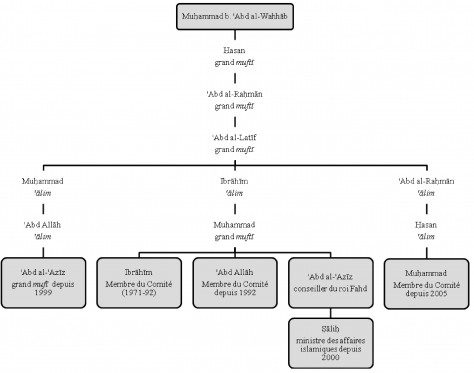
\includegraphics[width=\textwidth]{CourantsIslamContemporain/ImagesCourantsIslamContemporain/genealogie.jpeg}

13 Reste à signaler le cas particulier des oulémas originaires du Hijâz
et d'al-Aḥsā', provinces connues pour leur organisation hétéroclite. En
effet, la plupart des membres du Comité des grands oulémas, originaires
de ces régions, sont issus de ce qu'on a appelé des «dynasties»
d'oulémas, \emph{buyūtāt `ilm}, ou maisons de savoir comme ils aiment
eux-mêmes se faire appeler (à l'instar des familles d'oulémas dans les
autres pays arabes). Plus important encore est le fait que les familles
de ces oulémas appartiennent aux quatre écoles juridiques du sunnisme.
Si le facteur familial revêt une importance certaine, le paramètre de
l'origine tribale doit aussi être pris en compte.
\end{quote}

\hypertarget{la-pruxe9dominance-du-croissant-najdux12b}{%
\section{\texorpdfstring{La prédominance du croissant
\emph{najdī}}{La prédominance du croissant najdī}}\label{la-pruxe9dominance-du-croissant-najdux12b}}

\begin{quote}
14 Force est de constater que l'appartenance à une tribu, généralement
réinventée, constitue un critère identitaire important, dans une société
qui commence à peine à s'individualiser: avant d'être citoyen ou sujet,
on appartient d'abord à une tribu. C'est dire l'importance du milieu
tribal en tant que champ de socialisation des individus. La
\emph{`aṣabiyya}, l'esprit de corps tribal, joue un rôle fondamental
dans le statut social et la promotion de l'individu en Arabie Saoudite.

15 Les oulémas d'origine tribale dominent largement le Comité des grands
oulémas (il s'agit des tribus sédentarisées à partir du e siècle). Ils
sont quarante et un sur les cinquante-deux membres qu'a comptés le
Comité, depuis sa création, à être d'origine tribale, soit 79\%. Les
oulémas d'origine tribale se taillent ainsi la part du lion depuis 1971.
Les onze sièges restants sont occupés par des oulémas issus de trois
milieux différents: des membres de la notabilité citadine du Hijâz
(cooptés pour représenter les intérêts de leur région: on essaie de
choisir les plus «wahhabisés» et/ou quiétistes des oulémas du Hijâz),
des étrangers naturalisés (ils sont hanbalo-wahhabites, ont des talents
«exceptionnels» et ont défendu le hanbalo-wahhabisme et l'État) et des
citadins du Najd, sans affiliation tribale ou \emph{ḫaḍīrī}-s (ces
derniers ne doivent, en principe, leur ascension sociale qu'à leurs
compétences personnelles).
\begin{marginfigure}
\includegraphics[width=1.2\textwidth]{CourantsIslamContemporain/ImagesCourantsIslamContemporain/image10.jpeg}
\end{marginfigure}


16 On constate alors, chiffres à l'appui, que l'appartenance au milieu
tribal sédentarisé joue un rôle déterminant dans l'ascension sociale des
oulémas, la \emph{`aṣabiyya} étant une valeur ajoutée qui permet de se
constituer un capital social. Cela dit, bien que les tribaux dominent
largement en nombre le Comité des grands oulémas, ils ne sont

toutefois pas représentatifs du paysage tribal saoudien. En effet,
certaines tribus comme les Banū Tamīm, les Banū Zayd et les Banū Ḫālid
sont «surreprésentées», tandis que d'autres comme les `Utayba n'ont
guère droit, malgré leur importance numérique, qu'à un seul représentant
au Comité des grands oulémas. D'autres tribus enfin, comme les Šammar,
les Ḥarb, les Muṭayr, les `Ajmān, les Ġāmid, etc. n'ont aucun
représentant au sein du Comité. Si la marginalisation des Šammar, des
`Utayba et des Muṭayr peut s'expliquer par leur passé de tribus
frondeuses, la marginalisation des autres tribus ne peut, elle, être due
qu'à des facteurs religieux et surtout régionaux. Nous nuancerons
seulement, pour finir, en précisant que, dans certains cas, le charisme
personnel du \emph{`ālim} -- c'est le cas d'Ibn Bāz -- fait «oublier»
son appartenance tribale. En effet, ce \emph{`ālim}, citadin sans
affiliation tribale, a pu grimper jusqu'au sommet de l'establishment
hanbalo-wahhabite (il devient grand mufti et président du Comité des
grands oulémas en 1993), uniquement grâce à son «érudition», à son
intégrité morale et à son dévouement aux Sa‛ūd. Le charisme et le
pouvoir symbolique d'Ibn Bāz ont fait de lui le plus grand \emph{`ālim}
hanbalo-wahhabite contemporain.

17 Le royaume d'Arabie Saoudite est un royaume \emph{najdī}. Les élites
saoudiennes sont majoritairement originaires de la région de Najd, fief
de la dynastie et de la doctrine hanbalo-wahhabite. Des études plus
récentes (datant de la dernière décennie) se fondent sur des données
chiffrées mais ne portent que sur les élites ministérielles, la haute
fonction publique et les membres du Conseil consultatif. Rien donc sur
les oulémas. Nous tenterons, dans ce qui suit, de combler ce manque. Sur
les cinquante- deux membres du Comité depuis sa création en 1971, 73\%
des oulémas sont originaires du Najd; 9\% du Ḥijāz, 6\% du Sud, 4\% de
la région orientale et 7\% d'origine étrangère.
\begin{marginfigure}
\includegraphics[width=1.2\textwidth]{CourantsIslamContemporain/ImagesCourantsIslamContemporain/image11.jpeg}
\end{marginfigure}
 

18 Une majorité des membres du Comité des grands oulémas est donc
\emph{najdī} et ce depuis sa création. Deux remarques pourraient être
faites à ce propos. La première est que si l'on peut aisément comprendre
que seuls 4\% des grands oulémas sont des Aḥsā'ī-s puisque une grande
partie de la population de cette province est chiite ou sunnite autres
que hanbalo-wahhabite; si l'on peut aussi comprendre que seuls 9\% des
grands oulémas sont \emph{ḥijāzī} puisque, bien que sunnites, ils ne
sont, généralement, pas hanbalo- wahhabites, le chiffre de 6\% seulement
d'oulémas originaires du Sud de l'Arabie Saoudite peut, du moins \emph{a
priori}, paraître absurde puisque les habitants de cette région sont en
majorité hanbalo-wahhabites. L'hypothèse de la préférence régionale peut
être ainsi raisonnablement soutenue: si 73\% des grands oulémas sont
\emph{najdī}, c'est, justement, parce qu'ils sont originaires du fief du
hanbalo-wahhabisme et de la maison
des Sa‛ūd et que, de ce fait, leur soumission à l'un et à l'autre ne
peut être remise en cause. La seconde remarque est que si l'on compare
les chiffres avancés pour le Comité des grands oulémas à ceux que
présente le conseil des ministres au sein duquel les Najdī constituent
72\% des membres (Ibn Ṣunaytān, 2004: 70-73); à ceux du Conseil
consultatif où les Najdī sont majoritaires à 51\% (\emph{ibid}.: 93-96);
à ceux des ministres plénipotentiaires qui sont à 78\% originaires du
Najd ou encore, à ceux des hauts fonctionnaires qui comptent 67\% de
Najdī (\emph{ibid}.: 177-178), on voit que l'élite saoudienne étatique,
qu'elle soit religieuse ou politique, est majoritairement \emph{najdī}.
Les gens du Sud, eux, qui, comme on l'a dit, sont majoritairement
hanbalo-wahhabites, ne représentent que 1\% des ministres, 7\% des
membres de Conseil consultatif, moins de 5\% des ministres
plénipotentiaires et moins de 9\% des hauts fonctionnaires
(\emph{ibid}.: 177- 178): le même raisonnement peut être, ici,
développé. Le régionalisme primerait en Arabie Saoudite. Même si l'on
parle de saoudisation et de formalisation, l'État continue toujours de
s'appuyer sur l'élément najdo-wahhabite pour fonctionner.

19 Observons les chiffres de plus près: lorsque 9\% seulement des
oulémas sont originaires du Hijâz, 20\% des membres du conseil des
ministres, 29\% des membres du Conseil consultatif, 22\% des hauts
fonctionnaires sont \emph{ḥijāzī} (et 34\% parmi eux des cadres
supérieurs). Par ailleurs, en observant les chiffres de plus près
encore, il apparaît qu'au moment de la création du Comité, 29\% des
oulémas sont originaires du Hijâz contre 9\%, nous l'avons dit,
aujourd'hui. Le Comité tend donc, au fur et à mesure qu'il se met en
place et qu'il n'a plus besoin de cadres supérieurs, à se fermer à tout
ce qui n'est pas \emph{najdī}. Il faut ajouter à cela que les oulémas,
quand ils ne sont pas hanbalo- wahhabites, dissimulent leurs croyances
-- ou du moins évitent d'en parler -- et ne jouent, une fois admis au
sein du Comité, qu'un rôle de «figurants».

20 Le Comité des grands oulémas voudrait donner une illusion
d'ouverture: les principales régions sont toutes, même à une faible
proportion, «représentées». Actuellement, deux oulémas d'origine
\emph{ḥijāzi}, deux oulémas originaires du Sud et un autre de l'Est sont
membres du Comité des grands oulémas. En réalité, l'élément \emph{najdī}
domine toujours le Comité, et de loin; de plus, en supposant qu'il y ait
ouverture et même si le Comité accepte en son sein des chiites, il lui
suffirait de conserver une majorité de 51\% de hanbalo-wahhabites
(Najdī) pour que le vote à la majorité absolue passe au sein du Comité
et qu'ainsi, la vision hanbalo-wahhabite continue à dominer.

21 Enfin, en ce qui concerne les oulémas d'origine étrangère, ils ne
sont admis au sein du Comité (au nombre de trois) qu'au moment de la
création de ce Comité. Ces oulémas étrangers étaient, en effet, plus
compétents et plus qualifiés que les oulémas locaux; ils étaient dévoués
à l'État et au hanbalo-wahhabisme; nés non-wahhabites, ils l'étaient
devenus par conviction; ils n'avaient pas d'assise sociale et tribale en
Arabie Saoudite et devaient leur ascension à l'État; enfin, la
solidarité islamique, initiée par le roi Fayçal, entrait également en
ligne de compte. Depuis, le Comité s'est fermé aux étrangers et même les
enfants des dits oulémas étrangers ne sont pas admis au sein du Comité.

22 Le tracé reliant les villes du Najd dont les grands oulémas sont
originaires forme,
pour ainsi dire, un croissant que nous conviendrons d'appeler «croissant
\emph{najdī}» et qui constitue l'épicentre de l'Arabie Saoudite en même
temps que celui du hanbalo- wahhabisme. Il ne faut toutefois pas croire
que si les oulémas du Najd sont largement majoritaires au sein du
Comité, toutes les villes et les régions du Najd y seront équitablement
«représentées». Le Najd compte trois principales régions: la région de
Riyad qui a donné vingt-sept oulémas, le Qaṣīm dix et le Ḥā'il qui n'a
donné aucun \emph{`ālim}. Les deux régions, de Riyad et du Qaṣīm,
offrent un quasi-équilibre dans la répartition des oulémas: dans la
région de Riyad, en dehors de la ville elle-même, qui donne, à elle
seule, sept oulémas, les autres villes donnent, chacune, entre un et
quatre oulémas. De même, dans la région du Qaṣīm, le nombre d'oulémas
par ville varie entre un et trois.
\begin{marginfigure}
\includegraphics[width=1.2\textwidth]{CourantsIslamContemporain/ImagesCourantsIslamContemporain/image12.jpeg}
\end{marginfigure}
 

23 Le Ḥā'il, quant à lui, est volontairement marginalisé pour une raison
historique évidente: l'émirat du Ḥā'il a longtemps été le rival direct
des Saoud. Nous retrouvons à peine un représentant de cette région dans
le conseil des ministres et un seul autre au Conseil consultatif (Ibn
Ṣunaytān, 2004: 71 et 94).

24 Notons, pour finir, que certaines régions du Najd sont totalement
exclues et n'ont donné aucun \emph{`ālim}: l'exemple d'al-Dawādimī, pour
ne citer que lui, explique ce phénomène dans la mesure où la plupart des
habitants de la ville sont issus de la tribu des `Utayba dont la
fidélité au régime est douteuse. Il y aurait ainsi sous-régionalisation
à l'intérieur même de la régionalisation. De même, aucun grand
\emph{`ālim} n'est issu des régions du Nord. Enfin, aucun chiite n'est
admis au Comité des grands oulémas et ce, pour des raisons évidentes
qu'il ne semble pas utile de rappeler ici. Cela dit, les acquis familial
et tribal, seuls, ne suffisent pas: l'apprenti grand \emph{`ālim} doit
encore suivre un cursus d'études particulier pour intégrer le Comité.
\end{quote}

\hypertarget{de-la-ijux101za-au-doctorat-institutionnalisation-de-la-formation-du-ux101lim}{%
\section{\texorpdfstring{De la \emph{ijāza} au doctorat,
institutionnalisation de la formation du
‛ālim}{De la ijāza au doctorat, institutionnalisation de la formation du ‛ālim}}\label{de-la-ijux101za-au-doctorat-institutionnalisation-de-la-formation-du-ux101lim}}

\begin{quote}
25 Sur les cinquante-deux oulémas qui ont été membres du Comité des
grands oulémas depuis sa création, en 1971, 22\% (soit treize oulémas)
ont reçu une formation traditionnelle et 78\% (soit trente-neuf oulémas)
une formation «moderne». Près d'un quart des oulémas sont ainsi passés
par un cursus traditionnel. Nos entretiens nous permettent de décrire ce
\emph{ta‛līm} et d'en ressortir avec le cursus traditionnel «idéal
typique» du \emph{`ālim} hanbalo-wahhabite.

26 Au départ, entre l'âge de cinq et sept ans, l'apprenti \emph{`ālim}
fait son apprentissage du Coran. Les apprentis oulémas issus d'un milieu
modeste, ceux qui seront plus tard des self-made-men, apprennent le
Coran dans une école coranique (\emph{al-kuttāb}), aux mains d'un cheikh
de renommée moyenne. Les enfants des «cadres religieux moyens» et les
rejetons des dynasties d'oulémas, eux, apprennent le Coran auprès de
leur père, de l'un des membres de leur famille, ou d'un précepteur. On
imagine bien les difficultés rencontrées par les apprentis grands
oulémas issus de milieux modestes et le décalage qui se marque, dès le
départ, entre les apprentis oulémas issus des différentes classes
sociales.

27 Après cette phase d'apprentissage du Coran, l'apprenti \emph{`ālim}
doit, d'une part, commencer à étudier la grammaire et la rhétorique
arabes, de l'autre, apprendre par cœur les trois principaux ouvrages
d'Ibn `Abd al-Wahhāb sur l'unicité divine (\emph{al- tawḥīd}),
fondements du hanbalo-wahhabisme.

28 La troisième étape du cursus classique de l'apprenti \emph{`ālim} est
la quête du savoir
auprès des oulémas réputés. Le futur grand `ālim doit, en effet, réunir
un grand nombre de \emph{ijāzāt} (pl. de \emph{ijāza}: licences), dans
toutes les branches du savoir islamique disponibles, notamment en droit
et en théologie. Il assiste, pour ce faire, plus ou moins
assidûment, à des \emph{ḥalaqāt} `\emph{ilmiyya} ou cercles de savoir,
organisés quotidiennement dans les mosquées ou aux domiciles des
oulémas. Il s'agit alors, de séances de lectures mécaniques suivies de
commentaires d'ouvrages de hadith, d'exégèse coranique, de droit et de
théologie, notamment l'étude des œuvres classiques hanbalites. C'est à
l'issue de ces \emph{ḥalaqāt}, et une fois que l'étudiant a bien retenu
l'ensemble de l'enseignement dispensé par le \emph{`ālim}, qu'il fait un
\emph{istid`ā'}: une demande d'\emph{ijāza} pour les ouvrages étudiés.
Les étudiants les plus brillants deviennent assistants du maître et cela
leur ouvre la porte pour devenir professeur ou juge: la carrière est
alors lancée. Cela a été le cas de Muḥammad al-Sbayyil, le dernier grand
\emph{`ālim} à avoir reçu une formation traditionnelle.

29 Né dans la région du Qaṣīm vers 1926, al-Sbayyil est issu d'une
famille de «cadres religieux moyens». Son père, libraire et copiste
d'ouvrages religieux, connaît parfaitement le Coran. Son frère aîné,
`Abd al-`Azīz, est un \emph{`ālim} de la ville d'al- Bukayriyya. À l'âge
de cinq ans, al-Sbayyil commence son apprentissage du Coran auprès de
son père puis de son frère. Vers l'âge de dix ans, il se lance dans
l'apprentissage des trois ouvrages fondamentaux d'Ibn `Abd al-Wahhāb. Il
étudie aussi la jurisprudence hanbalite sous la direction des oulémas du
Qaṣīm, notamment les ouvrages d'Ibn Taymiyya (m. 1328), d'Ibn Qayyim
al-Jawziyya (m. 1350) et de Mar`ī al- Karamī (m. 1624), etc. À l'âge de
vingt ans, il aurait déjà acquis plusieurs \emph{ijāzāt} qui lui
permirent de devenir l'assistant du juge du Qaṣīm, `Abd Allāh b. Ḥumayd.

30 La formation traditionnelle indispensable au tout début du e siècle
perd, peu à peu, du terrain. En effet, les oulémas qui ont reçu cette
formation s'adaptent difficilement aux exigences de la modernité. 53\%
des membres du Comité des grands oulémas, soit neuf oulémas, ont reçu,
en 1971, une formation dite traditionnelle; en 2009, aucun grand
\emph{`ālim} ne bénéficie d'une telle formation. Dans un pays qui tente
de se moderniser, le besoin d'uniformisation de la formation des grands
oulémas s'impose. Il a fallu, pour y répondre, créer un cursus complet,
homogène, un cursus «national». Nous entendons par cursus moderne, un
cursus «institutionnalisé» et uniformisé.

31 S'ils ne sont que 47\% (soit huit oulémas), en 1971, à suivre la
formation dite moderne,
ils sont aujourd'hui 100\% à le faire. Après un cycle d'études primaires
dans des écoles publiques2\emph{,} les élèves qui se destinent à faire
une carrière juridico-religieuse, rejoignent les instituts de sciences
religieuses (\emph{al-ma`āhid al-`ilmiyya}). Le premier institut voit le
jour à Riyad, en 1950, à l'instigation du grand mufti du royaume de
l'époque, Muḥammad b. Ibrāhīm. Mais très vite, le gouvernement adopte le
projet et les instituts fleurissent dans toutes les régions du royaume
pour atteindre le chiffre de soixante- deux en 2009. Pour accéder à
l'enseignement de ces instituts, l'enfant doit avoir un dossier correct
et avoir appris au moins deux parties du Coran. L'enseignement y est
gratuit. Les instituts de sciences religieuses proposent un cursus de
six années: trois années de collège sanctionnées par un certificat de
réussite, sorte de «brevet» et trois années de lycée sanctionnées par un
certificat de réussite, sorte de «baccalauréat». Les matières étudiées
ont évolué depuis les années cinquante. Au début, l'enseignement était
constitué de quatre troncs communs: les sciences religieuses, les
sciences de la langue arabe, les «sciences sociales», et les
mathématiques. Au fil des années, on a ajouté à ce tronc commun d'études
de base, l'apprentissage obligatoire de la langue anglaise et de
l'informatique. Ces instituts de sciences religieuses sont inégalement
répartis sur l'ensemble du pays: le Najd compte 34\% des instituts, le
Hijâz 13\%, le Sud 28\%, le Nord 18\%, l'Est, enfin, 7\%. Les instituts
sont nombreux dans les régions où le hanbalo-wahhabisme est majoritaire
c'est-à-dire dans le Najd, le Sud et le Nord.

\begin{marginfigure}
\includegraphics[width=1.2\textwidth]{CourantsIslamContemporain/ImagesCourantsIslamContemporain/image13.jpeg}
\end{marginfigure}

32 Si la proportion entre le nombre d'instituts créés dans le Hijâz et
celui des oulémas qui sont admis au Comité des grands oulémas est
relativement équilibrée, la proportion entre le nombre d'instituts créés
dans les trois autres régions hanbalo-wahhabites et celui des oulémas
issus de ces régions et effectivement admis au sein du Comité, est,
quant à elle, largement déséquilibrée. On s'attendrait, en effet, à un
nombre plus important d'instituts de sciences religieuses dans le Najd,
à un nombre moins important dans le Sud et à un nombre nul d'instituts
dans la région du Nord. Or, ils sont créés dans le Nord et dans le Sud
mais ce, moins dans le but de former des grands oulémas que dans celui
de «wahhabiser» ces régions en y formant des techniciens du culte
hanbalo-wahhabite et des «cadres religieux moyens».

33 Lorsque l'apprenti \emph{`ālim} a terminé avec succès ses études
secondaires au sein de l'institut, il peut postuler pour les trois
grandes universités du pays: l'Université islamique de Médine (al-Jāmi`a
al-islāmiyya), l'Université islamique de la Mecque (Jāmi`at Umm al-Qurā)
et l'Université islamique de Riyad (Jāmi`at al-imām Muḥammad b. Sa`ūd
al-islāmiyya).

34 La première de ces universités, fondée en 1961, accueille surtout les
musulmans étrangers. Les Saoudiens qui y étudient se destinent
généralement à la prédication à l'étranger. De cette université n'est
issu qu'un seul grand \emph{`ālim}.

35 Quant à la deuxième citée, elle est la plus ancienne université de
théologie d'Arabie Saoudite, fondée en 1949. Elle n'a, malgré son
ancienneté, donnée que six grands oulémas. Doit-on y voir une
manifestation du régionalisme saoudien? Toujours est-il que cette
université accueille, depuis les années soixante-dix, des professeurs,
des cadres et des étudiants de diverses tendances politico-religieuses,
notamment des frères musulmans et des sahwistes (Lacroix, 2010: 47-97)
en lesquels le gouvernement saoudien et le Comité des grands oulémas
n'ont que très peu confiance et qui ne sont donc pas spontanément
recrutés par celui-ci.

36 La dernière université, enfin, est incontestablement la plus
importante pour notre étude. Elle a donné vingt-cinq oulémas, soit 51\%
des membres du Comité, depuis sa création en 1971, et 75\% des oulémas
ayant fait des études universitaires modernes. Cette université naît, en
1974, de la fusion de la faculté de théologie créée, elle, en 1953, et
de la faculté de langue arabe, créée en 1954.

\begin{marginfigure}
\includegraphics[width=1.2\textwidth]{CourantsIslamContemporain/ImagesCourantsIslamContemporain/image14.jpeg}
\end{marginfigure}

37 Depuis sa création, l'Université islamique de Riyad, qui,
rappelons-le, porte le nom du fondateur de l'émirat saoudien Muḥammad b.
Sa`ūd (1744-1765), fidèle allié d'Ibn `Abd al-Wahhāb, est considérée
comme le vivier des grands oulémas et de tous les cadres religieux et
techniciens du culte dont l'establishment religieux a besoin. Le
«pharaonique» campus de l'université (une véritable ville dans la ville
avec ses propres infrastructures, un petit hôpital, un supermarché, des
quartiers résidentiels pour les étudiants, les professeurs et le
personnel administratif, etc.) compte neuf facultés et deux instituts
supérieurs: la faculté de droit {[}musulman{]}; la faculté de théologie;
la faculté de langue arabe; la faculté des sciences sociales
{[}islamiques{]}; la faculté de la prédication et de la communication;
la faculté des langues et de la traduction; la faculté des sciences de
l'informatique; la faculté de l'économie; la faculté des sciences;
l'Institut supérieur de la magistrature et l'Institut de l'apprentissage
de la langue arabe {[}pour les étrangers{]}. Cela dit, les grands
oulémas sont exclusivement issus des facultés de droit et de théologie
et de l'Institut supérieur de la magistrature. Les étudiants dans ces
trois domaines bénéficient d'une bourse d'études et obtiennent, dès la
fin de leur première année d'études, le titre fort apprécié de
\emph{shaykh}. Le succès de l'Université islamique de Riyad est tel que
celle-ci s'est engagée dans une politique d'expansion en développant
deux filiales en Arabie Saoudite3 et cinq à l'étranger4\emph{.} Enfin,
certains étudiants peuvent préparer leur doctorat en sciences
religieuses à l'université égyptienne d'al-Azhar, pour le prestige que
cela donne. Une autre raison pourrait être avancée: certains apprentis
oulémas saoudiens iraient à al-Azhar pour observer l'organisation, les
structures et les mécanismes de fonctionnement de cette prestigieuse
université en vue de les
«importer» en Arabie Saoudite.

38 Les oulémas, au moment de leurs études supérieures, ont tous un tronc
commun tripartite: les fondements de la théologie (\emph{al-`aqīda});
l'exégèse coranique (\emph{al tafsīr}) et la jurisprudence
(\emph{al-fiqh}). À partir de la première année de master (calqué sur le
système anglo-saxon), 74\% des oulémas se spécialisent dans la
jurisprudence, et plus spécialement dans les fondements de la
jurisprudence islamique (\emph{uṣūl al-fiqh}) dans le but d'acquérir la
qualification requise pour émettre des \emph{fatwā}; 26\% d'entre eux,
se spécialisent en théologie, et plus précisément en religions comparées
(en réalité, pour dénigrer toute autre religion que l'islam
hanbalo-wahhabite)5\emph{.} Le choix de ces spécialisations n'est pas
étonnant dans la mesure où les étudiants se destinent avant tout à être
des techniciens du culte et des gestionnaires des biens de salut. Nous
n'entrerons pas, pour ne pas alourdir notre propos, dans le détail des
spécialisations pointues à l'intérieur même des deux grands domaines de
spécialisations que nous avons évoqués.

39 Bien que le cursus moderne se soit bien implanté dans le paysage
saoudien, l'ijāza
n'en demeure pas moins source de prestige et un élément non négligeable
dans un
capital social. Nous avons pu observer que la totalité des oulémas qui
ont suivi le cursus moderne ont, néanmoins, obtenu une ou plusieurs
\emph{ijāzāt}. Elément de prestige comme nous venons de le dire,
l'\emph{ijāza} est, en théorie, facultative. Mais, en pratique,
l'obtention d'une \emph{ijāza} permet au \emph{`ālim}, d'une part, de se
rattacher à une chaîne de transmission
«ininterrompue» d'oulémas remontant jusqu'au Prophète, ce qui permet au
\emph{`ālim} de légitimer sa position et son savoir et de s'inscrire
dans l'héritage prophétique, d'autre part, de nouer des relations
privilégiées avec un ou plusieurs oulémas et de commencer ainsi à tisser
un réseau qui pourra le mener au sommet de l'establishment hanbalo-
wahhabite.

\textbf{Faire carrière: le \emph{cursus honorum} des oulémas}

\begin{marginfigure}
\includegraphics[width=1.2\textwidth]{CourantsIslamContemporain/ImagesCourantsIslamContemporain/image15.jpeg}
\end{marginfigure}

40
L'enseignement et la magistrature ont toujours été les métiers de
prédilection des oulémas. Les membres du Comité des grands oulémas
n'échappent pas à cette règle. 96\% d'entre eux exercent au moins une de
ces deux professions: 50\% du Comité, soit vingt et un grands oulémas,
ont été ou sont encore, professeurs de jurisprudence islamique ou de
théologie; 31\% d'entre eux sont magistrats dans les différentes
instances de la justice saoudienne; 15\% des grands oulémas ont cumulé
les deux fonctions. À la question: «pourquoi le choix de ces métiers?»
Une première réponse, unanime, des grands oulémas magistrats: «la
justice est le fondement de la royauté». Et, selon les oulémas, qui,
mieux que des spécialistes de «la loi divine», pourraient mettre la
justice en application! Les grands oulémas ont d'ailleurs pleine
conscience de l'importance de leur mission. Ils ont une vision
catastrophiste d'un monde où le \emph{`ilm}, qui risque d'être perdu,
doit être sauvé, épuré des innovations blâmables et transmis par le
\emph{`ālim}.

41 En outre, si la magistrature permet au grand \emph{`ālim} d'observer,
d'analyser et de statuer sur des cas concrets, l'enseignement permet de
transmettre le savoir théorique. Cela, en plus du prestige qui entoure
ces deux fonctions. Il n'est, enfin, pas étonnant de voir que nombre de
grands oulémas cumulent les deux fonctions puisqu'en réalité, l'une et
l'autre sont indissociables (pratique et théorie). Ce phénomène de cumul
des fonctions (d'enseignant et de magistrat) est surtout visible dans la
première génération des grands oulémas. Il s'explique par le manque de
cadres religieux au moment de la
création du Comité. Les grands oulémas devaient donc assumer, tout à la
fois, leur rôle au sein du Comité et les fonctions de magistrats et
d'enseignants. Des années quarante aux années soixante, l'Arabie
Saoudite a été obligée d'«importer» des cadres religieux de l'étranger,
notamment de l'Égypte. Un exemple: l'Égyptien `Abd al-Razzāq `Afīfī (m.
1994), arrivé en Arabie Saoudite, en 1949, pour enseigner la langue
arabe et les sciences religieuses dans un collège à Tayef, a gravi, un à
un, les échelons et parvient au sommet de l'establishment religieux: il
est nommé, en 1971, au sein du Comité des grands oulémas. Cet exemple
révèle deux réalités: premièrement, l'Arabie Saoudite a fait appel aux
étrangers pour l'enseignement, à une certaine époque, à cause du déficit
de cadres dont elle a souffert dans tous les domaines; et deuxièmement,
les étrangers hanbalo-wahhabites, qui pouvaient aisément s'intégrer dans
le pays d'accueil, ont pu, à force de persévérance, atteindre le sommet
de l'establishment religieux saoudien.

42 La pratique du cumul des fonctions d'enseignant et de magistrat tend
à disparaître: le dernier grand \emph{`ālim} à avoir cumulé ces deux
fonctions est `Abd Allāh b. Qa`ūd, membre du Comité de 1977 à
19866\emph{.} Désormais, les grands oulémas, qu'ils soient professeurs
ou magistrats, sont de plus en plus spécialisés, chacun dans son
domaine: de professeurs de droit en général, ils sont devenus
professeurs de droit pénal, de droit de la famille, etc. Parallèlement à
ces deux métiers de prédilection, les grands oulémas sont techniciens du
culte: la plupart d'entre eux sont imâm dans les mosquées. Par exemple,
le grand mufti actuel du royaume, `Abd al-`Azīz āl al-Shaykh, est
également imâm de la grande mosquée de Riyad. Sāliḥ b. Ḥumayd est, lui,
imâm de la grande mosquée de la Mecque, etc. N'oublions pas enfin,
l'autre fonction essentielle des grands oulémas, celle d'«entrepreneurs»
de biens de salut, à savoir promulguer des \emph{fatwā} et se mettre à
l'écoute de la population. Mais si les grands oulémas monopolisent les
grands postes religieux et judiciaires saoudiens, ils n'hésitent pas à
empiéter sur le domaine réservé des autres élites.

43 Une fois admis au sein du Comité, le grand \emph{`ālim} obtient
automatiquement le grade de haut fonctionnaire (\emph{al-martaba
al-mumtāza}), voire celui de ministre. Sur les cinquante-deux membres du
Comité des grands oulémas, vingt-deux ont occupé des postes de
responsabilité autres que ceux de magistrats et d'enseignants. Déjà neuf
membres de la \emph{Hay'a} ont été ou sont encore ministres. Les
ministères que contrôlent les oulémas (si ce ne sont pas eux qui les
contrôlent directement, c'est un membre de l'establishment religieux)
sont ceux de la justice, des affaires islamiques, du pèlerinage et de
l'enseignement des filles (avant le rattachement de ce dernier, en 2002,
au ministère de l'éducation nationale). Depuis sa création, le ministère
de la justice est dirigé par un membre du Comité7\emph{.} Huit membres
du Comité des grands oulémas on été membres du Conseil consultatif: le
président de ce conseil, qui fait se côtoyer islamistes,
«libéraux», conservateurs et tribaux, depuis sa création, en 1992, est
un membre du Comité des grands oulémas. De 1992 à 2002, c'est Muḥammad
b. Jubayr, membre du Comité des grands oulémas (de 1971 à 2002), qui
assure la présidence de cette instance. Sāliḥ b. Ḥumayd, membre du
Comité des grands oulémas depuis 2001, lui succède en 2002. Ce dernier
est remplacé par `Abd Allāh Āl al-Shaykh, en 2009. Trois membres de la
\emph{Hay'a} ont été conseillers du roi Fahd (1982-2005) et deux sont
actuellement conseillers du roi `Abd Allāh. Quatre membres du Comité ont
occupé les postes de doyen ou de président d'université. Par exemple,
`Abd al-`Azīz b. Bāz occupe jusqu'à sa mort, en 1999, le poste de
président de l'Université islamique de Médine. Sa`d al- Ḍuwayḥī est
doyen de la faculté de théologie d'al-Aḥsā'. `Abd Allāh b. `Abd
al-Muḥsin al- Turkī, sans doute l'un des membres les plus actifs du
Comité, actuellement, occupe le poste de président de la Ligue islamique
mondiale, après avoir occupé, entre autres, les postes de président de
l'Université de Riyad et de ministre des affaires islamiques.

44 C'est dire que les oulémas ont adopté, depuis au moins deux
décennies, une stratégie adaptative qui les pousse à investir plusieurs
secteurs d'activités. Outre les domaines religieux, législatif et
éducatif, ils investissent les associations caritatives, les
organisations gouvernementales et non gouvernementales et les domaines
économique et financier. Dans ces deux derniers domaines, trois oulémas,
`Abd Allāh b. Manī`, `Abd
al-Wahhāb Abu Sulaymān et `Abd Allāh al-Muṭlaq se sont «improvisés»
experts et consultants incontournables dans les marchés financiers
saoudiens. Les trois hommes sont aussi membres de plusieurs conseils
d'administration de banques et d'entreprises dans le cadre de ce que
l'on appelle en Arabie Saoudite \emph{al-lijān al-šar`iyya} ou
commissions islamiques. Le nom-même d'un grand \emph{`ālim} sur la
brochure d'une société ou d'une entreprise est la meilleure des
publicités.
\end{quote}

\hypertarget{la-multiplication-des-ruxe9seaux-de-soutien}{%
\section{La multiplication des réseaux de
soutien}\label{la-multiplication-des-ruxe9seaux-de-soutien}}

\begin{quote}
45 Cette mobilité des oulémas n'est, toutefois, possible que si le
\emph{`ālim} tisse, autour de lui, un réseau sur lequel il peut
s'appuyer. Les capitaux culturel et économique doivent encore être
complétés par un réseau de soutiens. Nous avons pu observer trois types
de capitaux sociaux mobilisés par le futur grand \emph{`ālim}. Autrement
dit, le recours aux relations personnelles permet à ce dernier de
s'assurer une meilleure position dans la hiérarchie sociale. Ces trois
réseaux, que nous exposons séparément, sont en réalité, presque
toujours, combinés par le futur grand \emph{`ālim}. Le réseau familial
constitue la première ressource du futur grand \emph{`ālim}. Nous avons,
en effet, constaté l'existence d'au moins trois exemples de réseaux
familiaux qui sont autant de moyens d'accès au Comité des grands
oulémas.

46 Le premier est, sans aucun doute, le plus puissant et le plus dense:
celui des Āl al- Shaykh. Nous avons évoqué plus haut l'importance de
cette famille et nous tenterons, dans ce qui suit, de compléter le
tableau amorcé. L'exemple des deux fils, Ibrāhīm et `Abd Allāh, du grand
mufti Muḥammad b. Ibrāhīm est tout à fait significatif: bien que le
premier des deux ait été relativement peu brillant par rapport aux
collaborateurs de son père, il a quand même été nommé par ce dernier
vice-mufti du royaume d'Arabie Saoudite. Après la mort de son père et la
suppression du poste de mufti, Ibrāhīm, qui était destiné à devenir
mufti, reçoit, en guise de consolation, les postes de ministre de la
justice, de membre du Comité des grands oulémas et de président de la
Direction de la recherche scientifique, de la prédication et de
l'instruction! En 1992, lorsqu'Ibrāhīm se retire des affaires, son
remplaçant au ministère et au Comité des grands oulémas n'est autre que
son frère cadet `Abd Allāh, président actuel du Conseil consultatif. Un
autre exemple étonnant de la famille Āl al-Shaykh: il s'agit de Ṣāliḥ b.
'Abd al-`Azīz, le petit fils d'Ibn Ibrāhīm. Après avoir fait des études
scientifiques depuis le lycée et obtenu un diplôme d'ingénieur, Ṣāliḥ
décide de récupérer l'héritage familial et s'inscrit à l'Université
islamique de Riyad. Grâce à son nom et à l'intervention de son père, qui
était l'un des conseillers du roi Fahd, il obtient une équivalence et
passe ainsi directement en année de master: il contourne la règle qui,
aussi stricte soit-elle, s'efface quand il s'agit d'un Āl al-Shaykh. Il
est actuellement ministre des affaires islamiques et, potentiellement,
membre du Comité des grands oulémas. Un dernier exemple enfin de cette
famille: le dernier admis à Hay'at kibār al-'ulamā', Muḥammad b. Ḥasan,
fait une ascension fulgurante grâce à ses bonnes relations avec son
cousin, le grand mufti actuel d'Arabie Saoudite: il a pu, rapidement,
gravir les échelons universitaires et devenir le directeur de cabinet du
mufti. Ce dernier l'épaule et le soutient: il propose son nom au Comité
des grands oulémas auquel Muḥammad b. Ḥasan accède en avril 2005.
Signalons, enfin, que le réseau familial des Āl al-Shaykh et l'influence
qui en découle, dépassent largement le seul cadre religieux: un membre
de la famille est ambassadeur à Paris, un autre est directeur du
protocole royal, un troisième est membre de la chambre de commerce, etc.
Le deuxième réseau familial est celui des Ibn Ḥumayd, déjà présenté plus
haut.

47 Le dernier réseau familial, enfin, de moindre importance, est celui
des al-Šathrī: cette
famille du Najd a donné quelques oulémas et plusieurs hommes politiques.
`Abd al-‛Azīz al-Šathrī, un des conseillers des rois Fayçal (1964-75) et
Ḫālid (1975-82) a également été un ouléma de renommée moyenne. Son fils,
Nāṣir, a réussi à faire une brillante carrière politique (en tant que
conseiller des rois Ḫālid et Fahd). Selon un des
membres du clan al-Šathrī: «il ne manquait à {[}la{]} famille qu'un
grand \emph{`ālim} pour qu'{[}elle{]} devienne, enfin, une grande
famille». La parentèle met tout en œuvre pour que son rejeton prodige,
Sa‛d, accède au sommet de l'establishment religieux. Aussi, le
prépare-t-on, dès son plus jeune âge, à devenir grand \emph{`ālim} : on
le confie aux maîtres les plus compétents dans le domaine, tels Ibn Bāz,
Ibn `Uthaymīn, al-Aṭram, al-Rakbān et `Abd al-`Azīz Āl al-Shaykh. On le
pousse à s'inscrire à Jāmi'at al-imām où il obtient un doctorat en
fondements de la jurisprudence islamique. Sa`d brûle toutes les étapes
du \emph{cursus honorum} hanbalo-wahhabite et devient professeur de la
même université en un temps records. En mars 2005, la famille soutient
la candidature de son fils au Comité des grands oulémas (le père est
membre du cabinet royal qui transmet les candidatures au roi). Sa`d est
finalement nommé, en avril 2005: à trente-huit ans, il est le plus jeune
membre de l'histoire du Comité des grands oulémas.

48 Nous l'avons dit, le régionalisme et le segmentarisme dominent le
paysage politico- religieux saoudien. La deuxième ressource du futur
grand \emph{`ālim} est, naturellement, le réseau tribal qui va de pair
avec le réseau régional, autrement dit avec le réseau \emph{najdī}. Nous
avons remarqué, en analysant les origines géographiques et tribales des
grands oulémas, que ces derniers sont généralement issus des plus
grandes confédérations tribales du Najd: les Banū Ḫālid ont donné quatre
grands oulémas, les Banū Zayd, sept, les Banū Subay`, trois, les Banū
Tamīm, huit (auxquels il faut ajouter les quatre grands oulémas des Āl
al-Shaykh), les Qaḥṭān, trois, les `Unayza, trois, les Bāhila, deux et
al- Dawāsir, deux également. Soit un total de trente-six grands oulémas
issus des grandes tribus du Najd sur les cinquante-deux membres du
Comité. Le réseau tribal est très dense. Le nombre de grands oulémas est
plus ou moins bien réparti entre les grandes tribus \emph{najdī}. D'un
mouvement de nomination au sein du Comité à l'autre, cet équilibre est,
consciemment ou inconsciemment, maintenu. Exemple: les deux grands
oulémas, Muḥammad āl Sulaymān et Bakr Abū Zayd, de la tribu des Banū
Zayd -- admis tous deux au Comité, en 1992 -- sont remplacés, en 2005,
par deux hommes issus de la même tribu, `Alī al-Ḍuwayḥī et `Abd
al-Raḥmān al-Sadḥān. D'ailleurs, le réseau tribal doublé du réseau
régional ne concerne pas uniquement le champ religieux: on retrouve ces
mêmes configurations dans le domaine politico-administratif (Ibn
Ṣunaytān, 2004, 59-62).

49 La dernière ressource du futur grand \emph{`ālim} est la
\emph{mulāzama}: le fait de s'attacher un
long moment à un maître en sciences religieuses, réputé et influent.
Côtoyer un maître pendant plusieurs années permet à l'apprenti grand
\emph{`ālim} de nouer avec lui des relations personnelles qui peuvent
même aboutir au mariage de l'élève avec la fille ou la nièce du maître.
Par exemple, Ṣāliḥ al-Luḥaydān est, pendant plusieurs années, le
disciple favori du grand mufti Muḥammad b. Ibrāhīm. Cette relation
privilégiée lance véritablement la carrière de Ṣāliḥ qui devient le
gendre et le directeur de cabinet du mufti et qui gagne peu en peu en
charisme. Une année seulement après le décès du maître, al-Luḥaydān est
admis au Comité des grands oulémas; il hérite aussi de la fonction de
magistrat; quelques années plus tard, il devient le président du Haut
conseil de la magistrature, poste qu'il occupe jusqu'en février 2009.
Al-Luḥaydān est le doyen du Comité des grands oulémas dont il est membre
depuis 1971. Il en est aussi un des membres les plus influents. Il
serait, en effet, le seul à pouvoir opposer un veto pour la nomination
d'un nouveau membre: en 2005, il aurait utilisé son veto pour s'opposer
à l'entrée de l'ouléma `Abd al-Muḥsin al-`Ubaykān au Comité.

50 Un autre exemple: Muḥammad al-Sbayyil est le disciple d'Ibn Ḥumayd
alors que
celui-ci est le \emph{qāḍī} d'al-Bukayriyya. Quand Ibn Ḥumayd devient le
\emph{qāḍī} du Qaṣīm, il fait appeler al-Sbayyil à Burayda pour le
désigner professeur et responsable d'un institut de sciences religieuses
de la région. La relation entre les deux hommes est telle que,
lorsqu'Ibn Ḥumayd devient le grand juge du Ḥijāz, il le fait venir à la
Mecque et le nomme imâm de la grande mosquée de la Mecque et
vice-président de l'administration chargée de gérer les deux lieux
saints. Il finit même par en devenir président (jusqu'en 2005) après la
disparition de son protecteur. Depuis son arrivée à la Mecque, il tisse
des
relations étroites avec des oulémas et grands oulémas notamment Ibn Bāz
(qui n'est pas son maître) mais qui finit par lui proposer de devenir
membre du Comité en 1992.

51 Un troisième exemple: c'est également Ibn Bāz qui suit, pas à pas, la
carrière de `Abd
Allāh b. Qa'ūd qui est son meilleur disciple. À la première occasion (le
décès d'Ibn Ḥumayd et de Miḥḍār `Aqīl), Ibn Bāz propose le nom d'Ibn
Qa`ūd au cabinet royal qui le nomme membre du Comité en 1977.

52 Un dernier exemple enfin: le mufti actuel, `Abd al-`Azīz āl
al-Shaykh, en plus du réseau familial que lui confère son nom, bénéficie
du soutien de son maître Ibn Bāz. Il s'agit d'abord d'une question de
solidarité et de reconnaissance: Ibn Bāz est un \emph{mulāzim} du grand
père de `Abd al-`Azīz Āl al-Shaykh, Muḥammad b. `Abd al-Laṭīf. Il aide
donc `Abd al-`Azīz Āl al-Shaykh à devenir professeur à l'université
d'al-Imām, et propose son nom au cabinet royal pour en faire un membre
du Comité des grands oulémas (il le deviendra en 1987). En 1993, Ibn Bāz
devient mufti et désigne `Abd al-`Azīz āl al-Shaykh vice-mufti du
royaume et ce, bien que d'autres grands oulémas soient plus compétents
que lui. En effet, depuis les années soixante et jusqu'à sa mort, en
1999, Ibn Bāz occupe une position-clé dans l'establishment religieux. Il
bénéficie du respect et de la considération des autres grands oulémas et
exerce, de ce fait, une influence autour de lui, tous les grands oulémas
tenant compte de ses conseils et suivant à la lettre ses directives. La
centralité d'Ibn Bāz est ainsi très importante: un grand nombre de
chemins passent par lui. Dix-huit grands oulémas sont ses disciples et
certains d'entre eux lui doivent leur entrée au sein du Comité.
\end{quote}

\hypertarget{le-quiuxe9tisme-politique}{%
\section{Le quiétisme politique}\label{le-quiuxe9tisme-politique}}

\begin{quote}
53 En cherchant à identifier les conditions d'accès au Comité des grands
oulémas à travers le parcours de ses membres, nous avons constaté qu'il
existe deux critères directement liés à la vie politique et sociale:
aucun des grands oulémas n'a de passé politique (c'est-à-dire, une
quelconque manifestation d'opposition au régime: demande de réformes, ou
autres), et aucun \emph{`ālim} n'a jamais critiqué les décisions du
Comité ou de l'un de ses membres et ce, même si ses positions allaient à
l'encontre des décisions officielles.

54 `Abd Allāh Ibn Jibrīn, haut fonctionnaire religieux et candidat
potentiel au Comité des grands oulémas, a été l'un des parrains de la
contestation islamiste des débuts des années quatre-vingt-dix (Kepel,
2003: 335-337; Lacroix, 2007: 371-443). Ces actes constituent une
véritable offense tant pour le régime que pour les grands oulémas. Ces
derniers ne manquent pas, d'ailleurs, de le désavouer publiquement: il
est démis de ses fonctions officielles. Réhabilité par la suite, et bien
que très bon \emph{`ālim}, il ne pourra cependant jamais prétendre au
poste de grand \emph{`ālim} en raison de cette «bavure»: s'étant
ouvertement opposé au gouvernement et ayant participé à des activités
politiques allant à l'encontre des positions officielles, son «rachat»
et son récent soutien au gouvernement ne suffisent pas. Il ressort de
cet exemple que le quiétisme politique des candidats au Comité est un
élément fondamental et un critère-clé de sélection. Tout ce que peut
tolérer le Comité comme engagement politique pour un futur grand
\emph{`ālim} est le soutien aux décisions du pouvoir. `Alī al-Ḍuwayḥī
est l'exemple du \emph{`ālim} engagé politiquement -- en faveur du
régime bien sûr -- qui accède à la Hay'a. En effet, depuis 2001,
al-Ḍuwayḥī, qui dirige la faculté de théologie d'al-Aḥsā', a signé
plusieurs pétitions politiques défendant les programmes scolaires
saoudiens, et se déclarant en faveur de la tenue d'élections
municipales, etc.

55 Quant à `Abd al-Muḥsin al-`Ubaykān, qui a appelé ouvertement le
gouvernement à entreprendre des réformes, entre 1992 et 1994, il a été
marginalisé et démis de ses multiples fonctions: il perd son poste de
juge au tribunal de Riyad et d'imâm de mosquée. Réhabilité, dans les
années 1999-2000, il continue néanmoins à critiquer les décisions de la
Hay'a (surtout celles qui concernent la jurisprudence), et du système
judiciaire. Il émet même des \emph{fatwā} contredisant celles du Comité
des grands oulémas et
tente, pour se rattraper, de promulguer des \emph{fatwā} sur la licéité
du salut du drapeau national, sur la condamnation des sahwistes ou
encore sur l'interdiction du djihâd en Irak pour les Saoudiens. Le
gouvernement a accepté de le réhabiliter mais les oulémas ont opposé un
veto catégorique à l'entrée de ce \emph{`ālim} au Comité. Al-`Ubaykān a,
finalement, été nommé, dans un premier temps, conseiller au ministère de
la justice et membre du Conseil consultatif, avant de devenir l'un des
conseillers du roi, en 2009.

56 Les leaders de la \emph{ṣaḥwa} dans les années quatre-vingt-dix,
Safar al-Ḥawālī, Salmān al-`Awda et Muḥsin al-`Awājī, reconnaissent
eux-mêmes que l'un des critères d'accès au Comité des grands oulémas est
le quiétisme sur les plans politique et sécuritaire et acceptent donc,
du fait de leur très grand engagement politique, de ne pas y prétendre.

«Pour le gouvernement, dit al-Ḥawālī, les grands oulémas doivent être
des hommes apolitiques, des hommes qui ignorent tout de la politique».
Salmān al-`Awda ajoute que
«les futurs membres du Comité doivent être des hommes sans histoire(s)».
Pour Muḥsin al-`Awājī «l'accès au Comité obéit à des critères purement
sécuritaires».

57 Il découle de tout cela le «portrait idéal» du membre du Comité des
grands oulémas:
le grand \emph{`ālim} est hanbalo-wahhabite; il est issu d'une famille
de «cadres religieux moyens» ou d'une «dynastie» d'oulémas; il est issu
d'une grande tribu sédentarisée du croissant \emph{najdī}; il a effectué
des études auprès de maîtres réputés (cela pour le \emph{`ālim} qui suit
une formation traditionnelle) ou dans un \emph{ma`had `ilmī} puis à
l'université al-Imām de Riyad (pour le grand \emph{`ālim} qui a reçu une
formation moderne); il s'est spécialisé en jurisprudence islamique; il
est généralement professeur d'université (al-Imām) ou magistrat; il a en
moyenne vingt-cinq années d'expérience dans le domaine religieux; il
n'est pas engagé politiquement (s'il l'est, il ne doit l'être qu'en
faveur du régime).

58 La moyenne d'âge du grand \emph{`ālim} qui accède au Comité est de
quarante-sept ans. Il y reste en moyenne quinze ans. Et, si les
circonstances d'accès à la Hay'a sont difficiles à déterminer, les
circonstances de départ de la Hay'a sont, elles, tout à fait claires: le
grand \emph{`ālim} quitte le Comité s'il décède, bien évidemment, s'il
est gravement malade ou s'il a commis un acte jugé répréhensible par le
roi -- en 1992, quatre grands oulémas auraient refusé de signer une
\emph{fatwā} et ont été limogés.

59 Le renouvellement des membres du Comité des grands oulémas est
généralement associé à une période de crise ou de transition. Les
renouvellements de 1987 et de 2001 sont des renouvellements de
transition (plusieurs oulémas sont décédés ou gravement malades), les
renouvellements de 1992 et 2005 coïncident avec des moments de crise
(respectivement, les conséquences de la guerre du Golfe et celles du 11
septembre). Depuis la création de la Hay'a, il y a eu reproduction de
l'élite: il ne reste plus de la génération de 1971 que trois membres.
Nous constatons toutefois que l'élite des grands oulémas restreint
l'accès, même à des personnes qui rempliraient toutes les conditions
formelles pour accéder au Comité. Sans doute le prestige d'appartenir au
Comité des grands oulémas ne pourrait que diminuer si l'accès devenait
trop aisé. L'élite du Comité est donc fermée: cinquante-deux membres en
trente-huit ans.
\end{quote}

\hypertarget{conclusion}{%
\section{Conclusion}\label{conclusion}}

\begin{quote}
60 L'habitus, ainsi défini, des grands oulémas, fruit d'un
conditionnement historique et social, est générateur d'un comportement
adapté, consciemment ou inconsciemment, à la logique de l'espace
politico-religieux saoudien: soutenir le pouvoir politique et gérer le
marché officiel des biens de salut. Les larges prérogatives dont dispose
le Comité dans les domaines politique, social et religieux, à côté de sa
fonction fondamentale de bastion idéologique et d'usine à légitimer les
actions du gouvernement, justifient le contrôle par le pouvoir politique
de son ordre du jour et de son budget et conditionnent le choix, très
sélectif, de ses membres. Les grands oulémas, qui se définissent eux-
mêmes comme les oulémas du pouvoir, doivent être acquis au régime. Si
les origines sociales, le parcours éducatif et les réseaux de
socialisation favorisent l'émergence d'une élite fermée et dévouée au
pouvoir, la `\emph{aṣabiyya} régionale y est pour beaucoup. Le

Comité est, à l'instar des autres institutions du pays, trusté par
l'élément \emph{najdī} (plus de 70\% des membres des élites saoudiennes
sont \emph{najdī}): cette région n'est-elle pas le fief du
hanbalo-wahhabisme et de la dynastie régnante? Il s'agit enfin pour les
oulémas d'un dévouement objectif: les intérêts spirituels et temporels
de l'establishment religieux étant intrinsèquement liés à ceux du
régime, si ce dernier était mis à mal, la domination du
hanbalo-wahhabisme sur le territoire saoudien -- très éclectique
religieusement -- serait indubitablement remise en cause.
\end{quote}




\backmatter
\chapter{Liste des théologiens}

\section{Grands théologiens Musulmans}


\subsection{al-Ġazālī}

le joyau d'al-Ġazālī~: \emph{Le Tabernacle des Lumières}, traduit
par Deladrière, Paris, Seuil, texte très dense et très profond aux
implications nombreuses.
\cpageref{theol:AlGazali1,theol:AlGazali4,theol:AlGazali5,theol:AlGazali6,theol:AlGazali7,theol:AlGazali9,theol:AlGazali10,theol:AlGazali11,theol:AlGazali13,theol:AlGazali14,theol:AlGazali16,theol:AlGazali17,theol:AlGazali18,theol:AlGazali19,theol:AlGazali20,theol:AlGazali21,theol:AlGazali22,theol:AlGazali23,theol:AlGazali24}
\pageref{theol:AlGazali29}
\pageref{theol:AlGazali2}
\pageref{theol:AlGazali3}
\pageref{theol:AlGazali8}
%\pageref{theol:AlGazali31}
\pageref{theol:AlGazali25}
%theol:AlGazali31,theol:AlGazali32,theol:AlGazali33,theol:AlGazali34,theol:AlGazali35,theol:AlGazali36,theol:AlGazali37,theol:AlGazali38} 
%\label{theol:AlGazali1}
\section{Ibn Taymiyya}


 

C'est le très grand penseur (controversé) du 13\textsuperscript{ème}
siècle. Un certain nombre de ses ouvrages ont été traduits (souvent mal,
je sélectionne les meilleures traductions).


\emph{La lettre de Palmyre} traite de deux questions théologiques~: les
attributs divins et la prédestination~!

\includegraphics[width=1.27534in,height=1.63243in]{Images/image26.png}

-~Ibn Taymiyya, \emph{Réponse Raisonnable aux Chretiens ?} édité,
traduit et commenté par Laurent Basanese, sj., Ifpo, 2011.

-~Ibn Taymiyya, \emph{Musique et danse selon Ibn Taymiyya}: Le livre du
\emph{Samâ°} et de la danse (\emph{Kitâb al-Samâ° wa l-Raq.s}), Paris,
Vrin, 2000.

-~Ibn Taymiyya, \emph{Pourquoi les savants divergent,} Al-Hadith
éditions, 2012


Voir p. \pageref{ibn-taymiyya}.

\section{Autres théologiens classiques}
\paragraph{Ibn Hanbal}

\pageref{Theol:IbnHanbal1}

\paragraph{Ibn Salah}
Ibn Salah
\pageref{Ibnsalah1}

\paragraph{Ibn Khaldūn}
Le penseur andalou Ibn Khaldūn \pageref{theol:IbnKhaldun} 

\paragraph{Ibn Qutayba}
Ibn Qutayba -- si ce nom ne vous est pas encore familier, cela devrait
faire `tilt' car nous l'avons rencontré au début de cette leçon. Il a
écrit un Traité sur comment rendre compte et comprendre les divergences
dans le \emph{ḥadīṯ.} A-t-il été traduit en français~? La réponse est en
note 3 --
\pageref{Theol:IbnQutayba1}

\paragraph{Kalābāḏī}
  est un auteur persan, mort aux environs de 990. Cet ouvrage
cherche à réconcilier le soufisme et l'orthodoxie. 
\pageref{theol:Kalabadi}


\paragraph{ʿAlī Ṭanṭāwī} \label{theo:AliAlTawani}
{Ali Al tantawi est originaire d'une
famille de lettrés égyptiens qui a émigré à Damas à la fin du XIXème
siècle.


Il s'est opposé à l'impérialisme occidental dans les pays
arabes et, en particulier, à la présence de la France comme mandataire
en Syrie et celle de l'Angleterre en Irak. Après l'indépendance de la
Syrie, en 1947, ses positions contre le communisme, qu'il considère
incompatible avec l'Islam lui valent d'être menacé dans son propre pays.
En 1963, il quitte la Syrie pour l'Arabie Saoudite et devient
enseignant.
Extrêmement populaire dans son pays d'adoption, il a
présenté des programmes à la radio et à la télévision pendant un quart
de
siècle.}


\subsection{Ibn Toumart}
\label{IbnToumart}
\mn{E.B., « Ibn Toumart », in 23 | Hiempsal – Icosium, Aix-en-Provence, Edisud (« Volumes »,
no 23) , 2000 \url{http://
encyclopedieberbere.revues.org/1629}}


Ibn Toumart est la personnalité religieuse et politique la plus marquante du Maghreb au
XIIe siècle. Fondateur du mouvement almohade*, il devait préparer la revanche des Sanhadja
montagnards contre l’empire déjà vacillant des Almoravides. Bien que ses disciples aient
manipulé sans vergogne sa généalogie pour le rattacher à la descendance du Prophète et en
faire, donc, un chérif, il est sûr qu’Ibn Toumart était issu d’une tribu du Sous, celle des Hergha,
appartenant au groupe montagnard des Maçmouda.
 L’un de ses premiers disciples, le pieux el Baïdaq, se fit son chroniqueur et grâce à son
récit, souvent dithyrambique, il est possible de saisir l’évolution spirituelle de celui qui
devait mériter le titre de Mahdi Almohade et le qualificatif d’Impeccable. Célèbre dès son
adolescence, pour son zèle religieux et son érudition qui lui avait fait donner le surnom d’asufu
(le tison, le flambeau, en berbère), Ibn Toumart quitta un beau jour son village d’Igliz et
ses montagnes pour compléter, en Orient, sa connaissance de l’islam et jeter les bases d’une
réforme radicale.
 Son séjour en Espagne n’est pas assuré, mais demeurent des concordances étroites entre
les textes d’Ibn Hazm et ses propres propositions. En revanche, sa présence à Bagdad est
pleinement confirmée, alors que son passage à Damas est peut-être légendaire et les entretiens
qu’on lui prête avec Ghazali certainement inventés.
 Dix ans après son départ d’Igliz, Ibn Toumart entreprend un long voyage de retour au Maghreb,
au cours duquel il multiplie les étapes, passant par Alexandrie, Tripoli, Mahdia, Tunis,
Constantine et Béjaia. Sa condamnation des moeurs citadines relâchées provoque souvent des
échauffourées. A Béjaia, ses violences verbales déclenchent la fureur populaire contre lui. Le
sultan hammadite, qui l’avait d’abord bien accueilli, lança ses sicaires à sa poursuite, mais Ibn
Toumart trouva refuge dans la tribu voisine, celle des Beni Urigol, dans le village de Melala.
\paragraph{
La doctrine almohade}
 Ibn Toumart y élabore sa doctrine et réunit ses premiers disciples. Le plus cher à son coeur,
celui qu’il considère comme l’homme providentiel qui doit lui succéder, est Abd el Moumen,
le fils d’un potier de Nédroma (Algérie occidentale). El Baïdaq nous a laissé le récit émouvant
de la désignation du futur calife. Le réformateur proclama un soir en prenant sa main : “La
mission sur laquelle repose la vie de la religion ne triomphera que par Abd el Moumen ben Ali,
le flambeau des Almohades.” Celui-ci, en pleurant, dit avec humilité : “Ô Maître, je n’étais
nullement qualifié pour ce rôle, je ne suis qu’un homme qui cherche ce qui pourra effacer ses
péchés.” – “Ce qui te purifiera de tes péchés, répondit Ibn Toumart, ce sera précisément le rôle
que tu joueras dans la réforme de ce monde.”
 Une conversation avec deux pèlerins de l’Atlas qui passaient par Bougie est l’occasion du
départ des premiers Almohades vers le Maghreb el Aqsa. La petite troupe, d’une dizaine de
personnes, gagne Marrakech non sans avoir semé la bonne parole et causé quelques troubles
dans les villes traversées : Tlemcen, Oujda, Taza, Fès, où Ibn Toumart se fait remarquer par
le saccage des magasins des marchands de musique, contre lesquels il semble avoir eu une
aversion certaine. Il réitère à Marrakech, brisant à coups de bâton instruments de musique
et jarres de vin, pourchassant sous les huées la soeur de l’émir almoravide, qui chevauchait
dévoilée dans les rues de la capitale.
 Après la prise de Tin Mel (1123), il se proclame Mahdi et, de retour dans les tribus Masmouda,
ses frères de race, il organise solidement la communauté almohade avec un soin et une
connaissance des hommes qui font de ce clerc un grand homme d’État. Il crée un véritable
État montagnard, solidement organisé, disposant d’une armée fanatisée chargée de répandre
la doctrine almohade jusqu’en Ifriqiya et en Espagne.

Nous retrouvons dans cette réforme la même tendance innée vers le rigorisme moral et la
simplicité doctrinale que nous ont révélés tous les schismes et hérésies nés en Berbérie à travers
les siècles.
Dans la condamnation absolue des richesses de ce monde et de ses frivolités, c’est la voix
d’Ibn Toumart qui tonne, mais elle fait écho à celle, non moins véhémente, de Tertullien. La
lente marche des Berbères vers le Dieu unique semble ici se parachever dans la proclamation
de l’Unicité absolue de Dieu, dont Ibn Toumart rejette jusqu’aux adjectifs (le Puissant,
le Miséricordieux, le Victorieux) que lui dorment les musulmans, parce qu’ils risquent de
faire apparaître comme divisible la puissance divine. La conséquence inévitable de la toutepuissance
de Dieu ainsi comprise est la prédestination de tous les êtres créés : chacun doit
attendre dans la soumission totale ce qui lui a été assigné de toute éternité.
Cette forme de l’islam ne peut qu’être fanatique, elle ne supporte ni relâchement des moeurs,
ni relativisme dans le dogme, ni présence d’Infidèles.
11 Ces données concordaient trop bien avec l’intransigeance fondamentale des Berbères pour ne
pas aboutir : aussi, sous Abd el Moumen, le raz de marée almohade balaya le Maghreb de
toute impureté. C’est alors, semble-t-il, que disparurent les dernières communautés chrétiennes
autochtones.
\paragraph{L’État almohade}
Respectueux des traditions tribales des Berbères du Haut Atlas, Ibn Toumart organisa son
gouvernement en établissant une hiérarchie entre différents conseils imités des assemblées
tribales. Au sommet siège le Conseil des Dix, qui sont les premiers et les plus fidèles
compagnons (Abd el-Moumen*, Abou Hafs Omar*, El Bachir...). Au-dessous du Conseil
des Dix, le Conseil des Cinquante est composé de contribules d’Ibn Toumart, des Hergha et
d’autres Maçmouda de Tin Mel ou des Hintata. Les différentes tribus de la montagne étaient
ainsi représentées dans ce Conseil dont les pouvoirs étaient restreints.
Toute la société almohade était strictement hiérarchisée. A l’intérieur des groupements
ethniques apparaissait une autre hiérarchie, fondée sur les fonctions exercées, depuis celles
des compagnons les plus proches jusqu’à celles confiées aux abid (serviteurs noirs). Au
sommet de la pyramide, le Mahdi tenait solidement les rênes d’un pouvoir absolu. Cette
domination reposait sur une logique implacable : tout Almohade suspecté de tiédeur risquait
l’élimination : ainsi lors de la “journée du tri” plusieurs milliers d’almohades “infidèles” furent
massacrés. C’est par de telles actions qu’Ibn Toumart réussit à construire l’État almohade et à
assurer la naissance de la nouvelle dynastie moumenide. Seuls le prestige et la volonté d’Ibn
Toumart réussirent à faire admettre Abd el-Moumen comme le successeur désigné du Mahdi.
Encore fut-il nécessaire de cacher la mort de celui-ci pendant plus de deux ans avant de faire
reconnaître le nouveau souverain par les Cheikhs almohades.
\paragraph{références}
voir p. \cpageref{theol:IbnTumart1}

\section{Théologiens modernes}
\subsection{Tarik Ramadan}
 \begin{itemize}
  \item Paradoxe de Tarik Ramadan~: dire que le radicalisme vient de
    l'occident. Et ensuite, valoriser le communitarisme pour refuser les
    coutumes locales et en particulier celles de la laicité.
  \end{itemize}
  
Voir réflexion sur le moratoire.
  
\section{Théologiens libéraux}

\paragraph{Mohammed Arkoun}
Savant à la pensée profonde, Mohammed Arkoun (1928-2010) était également un intellectuel engagé. Son analyse serrée des processus à l’œuvre dans l’islam d’hier était indissociable de ses appels répétés à une réforme des sociétés islamiques contemporaines. Il n’a cessé de porter ce message dans les divers colloques où il était convié, y compris là où l’on ne s’attendrait guère à croiser un islamologue : à un congrès de psychanalystes lacaniens, dans des conférences sur la condition féminine…
Il a choisi de consacrer les dernières années de sa vie à retravailler les textes issus de ces rencontres. Traitant de la nécessité de la réforme, voire de la « subversion » de l’islam, de l’ouverture lacanienne à la parole et à la « raison émergente », de la condition féminine en islam ou encore du rapprochement entre sunnites et shî‘ites, ils montrent combien la pensée de Mohammed Arkoun est plus que jamais féconde pour penser notre époque.
Voir  \cpageref{theol:Arkoun1,theol:Arkoun2} 
\label{theol:Arkoun3}

\paragraph{Rachid Benzine}.
Islamologue et historien, Rachid Benzine s’est intéressé à ces questions après sa rencontre avec le prêtre catholique Christian Delorme à Lyon et a beaucoup travaillé avec des théologiens protestants.



\section{Islamologues}

\subsection{Louis Massignon}


L’islamologue Massignon s’est avant tout situé dans la grande lignée des études sur l’Islam orthodoxe, son premier souci étant de démontrer que l’Islam a une dimension mystique et que c’est l’Islam sunnite essentiellement qui se prête à cette dimension. Mais que ce soit à travers son thème de recherche principal, Ḥallāğ, ou dans le reste de son œuvre, dans ses cours au Collège de France et à l’École des Hautes Études, dans ses incessants déplacements en Iran, en Syrie, au Liban, il s’est heurté au šī‘isme à tous les carrefours.

  \paragraph{Mansur al-Ḥallāğ pour Massignon} figure du Christ de l'Islam.

  Dieu demande à toutes les créatures devant l'homme. Une créature
  refuse. Traditionnellement, c'est considéré comme un refus
  d'obeissance de l'ange (c'est de la boue puante~»). Pour al Hallaj
  c'est uniquement devant Dieu et c'est une épreuve de Dieu, c'était
  révélé à l'ange ce qu'est Dieu. Dieu est dans l'homme.
  \url{https://www.youtube.com/watch?v=Let1X-8zsXU\&t=1428s}
  C'est à cause de cette divinisation qu'il sera condamné, hétérodoxe.

\paragraph{Pierre Lory}
\label{Theol:PierreLory}
Un des grands connaisseurs de Qušayrī est
Pierre Lory.

Même en dehors des cercles salafistes, nombreux sont aujourd'hui les
musulmans~

\begin{cite}
« qui voudraient que le Coran soit un discours unique,
et qui se méfient des interprétations différentes les unes des autres
»,~
\end{cite}
\emph{}déplore~{{Pierre
Lory}}. Cet islamologue a contribué au récent site {{Coran 12-21}}
Internet~\url{https://coran12-21.org/fr/} , qui
présente différentes versions du Coran, dans trois langues différentes.

Pour lui, comme pour d'autres spécialistes, considérer le Coran comme un
tout dogmatique et intouchable est non seulement dangereux, mais aussi
erroné.

\paragraph{Abdessamad
Belhaj}
\begin{cite}
« La lecture littérale est en elle-même une
interprétation, puisqu'elle est fondée sur la prémisse que les propos du
Coran sont généralisables et peuvent faire fi des circonstances
particulières »,~
\end{cite}
remarque
l'islamologue~{\underline{Abdessamad
Belhaj}}, chercheur au Centre interdisciplinaire d'études de l'islam
dans le monde contemporain de l'Université catholique de Louvain.

\subsection{Autres Islamologues - IDEO}
\paragraph{Emmanuel Pisani}
Frère dominicain et islamologue, Emmanuel Pisani est directeur de l’Institut de Science et Théologie des religions (ISTR) à l’Institut catholique de Paris.

\paragraph{Adrien Candiard}



\section{Matériel d'Etude}\label{matuxe9riel}

\url{https://www.onelittleangel.com/livres/sacres/le-saint-coran.asp}

\url{https://coran.oumma.com/sourate/20} . Conseillé par Emmanuel
Pisani.

\url{https://www.lexilogos.com/clavier/arabe_latin.htm}

\url{https://referenceworks.brillonline.com/browse/encyclopedie-de-l-islam}

\url{https://www.lexilogos.com/coran.htm} : lexilogos y compris mot à
mot




\section{Notes diverses à repositionner}







Important de connaître un auteur pour avoir un avis objectif.





\begin{itemize}
\
  
\item
  Est-ce que j'utilise la raison, l'analogie, la coutume locale~? c'est
  cela les différences.
\item
  Si la coutume est la laicité, je dois en tenir compte pour mon avis.

  \begin{itemize}
  \item
    Le shavinisme qui intègre le ur, la coutume,
  \item
    le hanafisme, aussi~
  \item
    la où on le ferait moins, c'est le hanbalisme.
  \end{itemize}
\end{itemize}



  Pour quitter l'Islam, la peine est celle de la Loi locale. En France,
  si on définit l'islam comme une loi, on dit son aversion. Tout le
  chapitre sur la loi, «~islam = loi~», est un schématisme redoutable.
  Ce n'est pas qu'un texte législatif. Malheureusement, il y a tout un
  courant dans l'Islam qui encourage cette lecture caricaturale. Dans
  les pays occidentaux, on peut combattre avec les idées l'islam
  radical.
  
  
  \subsection{Islam compliqué}


Rachid Benzime

Islam, compliqué à lire le coran sans clé herméneutique

Passé colonial~en France~:

champ sémantique~: passer d'un champ indigène, à immigré, à ~musulman.
La religion devient le marqueur identitaire.

Pisani~:

Compliqué l'islam~; islam~: complexe

Edgar Morin~: c'est quoi la complexité d'un fait social. Si complexe,
reponse complexe

Ici, les arrières pensées~: on croit connaitre de l'islam alors que ce
n'est qu'une réalité.

Les musulmans comme «~citadelles assiégées~»

Difficile pour les musulmans de voir une certaine réalité car l'islam
quelque chose de beau.

«~un terroriste qui se dit musulman, on n'a pas le droit de lui dire
qu'il n'est pas musulman~»

Derrida~: «~il faut bien séparer l'Islam de l'Islam~».

Accepter que l'islam est pluriel, alors que l'islam est vécu par les
personnes comme unique.

Pisani~:

Macron~: l'islam est en crise.

Ce n'est pas possible pour les musulmans~: «~l'islam ne peut pas être en
crise~» - méta religieux.

Mohammed Arkoun~: le fait islamique. Dieu est absent.

Trop de représentations dans le champ «~Islam~». Mot trop chargé.

What is Islma.

\section{Le Coran peut-il être interprété ?}

 

Considéré par la plupart des musulmans comme un livre « incréé », et
donc parfois intouchable, le Coran a fait l'objet, au Moyen Âge, d'une
tradition de commentaires d'une grande profusion. 

\begin{itemize}
\item
  Mélinée Le Priol,~
\end{itemize}


Plusieurs anecdotes transmises par la tradition islamique montrent un
croyant venant consulter le prophète Mohammed sur le sens de tel ou tel
verset.

\subsection{Pourquoi l'interprétation du Coran est-elle un sujet sensible
?}

Synonyme de « récitation »,~\emph{Al Qur'an}~(en français le Coran)
contient, selon la tradition islamique, la révélation reçue par le
prophète de l'islam Mohammed, entre 610 et 632. L'ange Gabriel lui
aurait dicté les versets tels quels, et ceux-ci auraient été mis par
écrit une vingtaine d'années après la mort du Prophète, qui n'aurait
fait que les réciter à ses compagnons. Malgré son statut bien connu
de~\href{https://www.la-croix.com/Religion/Islam/Comprendre-Coran-2016-06-10-1200767802}{\underline{livre
« incréé »}}, le Coran a été abondamment étudié et commenté.

\emph{« Le courant littéraliste, qui considère que le Coran se suffit à
lui-même, que ses ambiguïtés sont voulues par Dieu et que l'interpréter
est source d'égarements, a toujours existé, mais il a longtemps été très
marginal en islam »,}~rappelle l'historien Mohammad
Ali Amir-Moezzi 
 . C'est depuis une cinquantaine d'années, avec
l'essor du salafisme, que cette conception a gagné du terrain,
valorisant essentiellement l'apprentissage par cœur.
 
 

\subsection{ Quelle est l'histoire du commentaire coranique ?}

Plusieurs anecdotes transmises par la tradition islamique montrent un
croyant venant consulter le prophète Mohammed sur le sens de tel ou tel
verset. Il faut dire que le texte coranique est un corpus
particulièrement ardu, au contenu souvent allusif, parfois
contradictoire. Non content d'entremêler des thèmes et registres
différents, il n'a pas été agencé selon l'ordre chronologique de la
révélation.

 
D'où la nécessité de l'interpréter. Riche de plusieurs milliers de
volumes, le commentaire du Coran a connu son âge d'or du
VIII\textsuperscript{e}~au XII\textsuperscript{e}~siècle.\emph{~« Les
grands courants de pensée islamiques se sont tous développés à partir de
la même interrogation : comment comprendre l'écriture sainte
?,~}explique Mohammad Ali Amir-Moezzi.\emph{~­L'islam a hérité de cette
culture exégétique des milieux bibliques au sein desquels il s'est
développé. »}

Les commentateurs ne pouvaient toutefois pas interpréter le Coran à leur
guise. On dénombre trois méthodes principales : la traditionnelle avait
essentiellement recours aux sources scripturaires (le Coran et les
hadiths) et à des analyses sur la langue arabe et la culture tribale ;
la rationnelle faisait appel à la logique et à la pensée spéculative, la
logique aristotélicienne ; et la mystique reposait sur une~\emph{«
illumination »}.

 

\emph{« Une posture postmoderne veut que le Coran soit dorénavant ouvert
à toute interprétation,~}s'inquiète Abdessamad Belhaj.\emph{~Mais cela
ne doit pas être une excuse pour ne pas explorer l'intelligence interne
du texte lui-même. »}~Le lecteur contemporain du Coran doit tout de même
recouvrer son~\emph{« autonomie »,}~reconnaît-il toutefois, regrettant
que l'abondante littérature produite dans les siècles passés ait pu
être~\emph{« sacralisée »}.

\subsection{► Comment renouveler l'interprétation du Coran au
XXI\textsuperscript{e}~siècle ?}

Si la~\emph{« quasi-totalité »}~des commentaires du Coran se font,
encore aujourd'hui, dans le registre traditionnel,~\emph{« on sent
depuis trois décennies les frémissements d'une nouvelle exégèse, qui
recourt davantage aux méthodes académiques occidentales »,~}observe
Mohammad Ali Amir-Moezzi. Non confessante, cette islamologie née dans le
monde occidental commence à trouver un écho dans des pays musulmans
comme l'Iran, la Tunisie ou la Turquie.

 

Pour ces chercheurs, l'enjeu est de ne plus seulement étudier le Coran à
partir des sources musulmanes datant d'au moins un siècle et demi après
la mort de Mohammed, mais de recourir aussi aux sources non musulmanes
(notamment juives et chrétiennes) du contexte religieux de l'Antiquité
tardive au sein duquel le Coran a émergé. Longtemps restées cloisonnées,
ces deux approches -- confessante et scientifique -- pourraient bientôt
se réconcilier.

Islam, pourquoi cette sévérité avec les autres croyants et les
incroyants ?

\emph{Explication~}

« Mécréants », « infidèles » : les terroristes islamistes s'en sont pris
violemment, ces dernières années, à tous ceux qu'ils jugent hors de
l'islam « authentique ». Une intolérance fondée sur une lecture
littérale du Coran. 

\begin{itemize}
\item
  Mélinée Le Priol,~
\item
  le~28/01/2021 à 13:04~
\item
  Modifié le~28/01/2021 à 13:12
\end{itemize}

Lecture en 3 min.

\includegraphics[width=6.3in,height=4.20208in]{media/image4.jpeg}

Selon la théologie musulmane, l'islam est la religion originelle de
l'humanité.VICTOR MOUSSA - STOCK.ADOBE.COM

\subsection{► Que dit la tradition ?}

Selon la théologie musulmane, l'islam est la religion originelle de
l'humanité.~\emph{« Tout homme est né musulman »,}~dit un hadith
attribué
au~\href{https://www.la-croix.com/sacralite-prophete-lislam-2020-11-06-1101123195}{\underline{prophète
Mohammed}}. L'homme est né pour adorer Dieu : certes, il a reçu une
dignité plus haute que les autres créatures, mais celle-ci est
conditionnée à sa soumission au Dieu unique. Plus un homme applique la
loi divine (\emph{charia}), plus il devient humain. Quant au « mécréant
» (\emph{kâfir}), qui refuse de suivre la charia, il se situe en quelque
sorte à un degré inférieur d'humanité.

Cette sévérité envers les non-musulmans s'appuie sur la lecture du texte
coranique qui s'est imposée à partir du IX\textsuperscript{e}~siècle,
lors de la transformation de l'islam en un empire soucieux de se
légitimer. Confortée par des hadiths rédigés à cette époque, elle
dépeint une vérité unique et non négociable. Elle insiste sur les
versets du Coran particulièrement virulents envers les polythéistes,
païens ou idolâtres, qualifiés d'\emph{« associateurs
»}~(\emph{mouchrikoun}) car ils « associent » à Dieu d'autres divinités.

Quant aux athées,~\emph{« ils appartiennent, selon la théologie
musulmane, à une catégorie de mécréance encore inférieure aux
polythéistes, aux juifs et aux chrétiens »,~}explique l'islamologue
Abdessamad Belhaj, chercheur au Centre interdisciplinaire d'études de
l'islam dans le monde contemporain de l'Université catholique de
Louvain. Même si des institutions comme le Haut Conseil des oulémas du
Maroc ou la Maison de la fatwa en Égypte considèrent que les apostats ne
peuvent plus être condamnés à mort, cette peine reste appliquée dans une
dizaine de pays, comme l'Afghanistan ou
la~\href{https://www.la-croix.com/Monde/Afrique/prisons-Mauritanie-calvaire-dun-apostat-2019-09-30-1201051050}{\underline{Mauritanie}}.

\subsection{ Pourquoi juifs et chrétiens bénéficient-ils d'un statut
spécifique ?}

Selon la tradition musulmane, chrétiens et juifs font l'objet d'un
traitement différent des autres non-musulmans : ils bénéficient dans le
droit islamique d'une protection juridique particulière (\emph{dhimma})
toutefois accompagnée d'injonctions humiliantes, comme l'interdiction de
monter à cheval ou de construire des lieux de culte dépassant ceux des
musulmans.
 

\emph{« Le Coran est très ambivalent au sujet des ``gens du Livre''
»,~}rappelle
l'historien~\href{https://www.la-croix.com/Culture/Livres-et-idees/historiens-decryptent-Coran-avant-lislam-2019-11-27-1201063090}{\underline{Guillaume
Dye}}, professeur à l'Université libre de Bruxelles (1). Selon la
sourate 5, juifs et chrétiens ne doivent pas être pris pour~\emph{«
alliés »~}(5, 51) mais, quelques versets plus loin, on lit qu'ils ne
seront~\emph{« point affligés »~}(5, 69). Les chrétiens se voient
reprocher de nier l'unicité de Dieu mais du respect est exprimé pour les
prêtres et les moines, qui~\emph{« ne s'enflent pas d'orgueil ».}

Selon une théologie dite de la falsification (\emph{tahrif}), les juifs
et les chrétiens ont altéré le message transmis par leurs prophètes
respectifs (Moïse, Jésus), message qui n'était autre que l'islam. Le
Coran, lui, corrige cette déviation en transmettant fidèlement le
message révélé à un ultime prophète, Mohammed. À Médine, celui-ci aurait
signé une~\emph{« Constitution »~}disposant que les juifs, notamment,
pouvaient pratiquer leur religion en sécurité, mais ces relations se
sont rapidement détériorées.

\subsection{► Quelles pistes pour une « théologie du pluralisme » ?}

Les attentats visant des « mécréants » en terrasse à Paris, les
persécutions contre les Yézidis ou les chrétiens en Irak, sont autant de
conséquences d'une lecture littéraliste du Coran encouragée par l'essor
du salafisme saoudien à partir des années 1970. D'autres lectures ont
pourtant existé dès les premiers siècles de l'islam. Contrairement à la
doctrine sunnite traditionnelle, l'exégèse rationaliste a par exemple
conclu très tôt à une~\emph{« égalité entre tous les êtres humains, tous
étant dotés de la même raison les rendant aptes à comprendre la parole
de Dieu »,~}rappelle l'islamologue Pierre Lory, directeur d'études à
l'École pratique des hautes études (EPHE).

Pour Abdessamad Belhaj, tout l'enjeu est aujourd'hui de refonder le
rapport à l'altérité sur la base de l'éthique, et de\emph{~« mettre
l'homme au cœur de la théologie »}. Pour cela, certaines valeurs
présentes dans l'islam gagneraient à être redécouvertes, comme celles du
soin, du don et du service à l'humanité, longtemps éclipsées selon lui
par l'autorité et la loyauté à la communauté musulmane ou à la tribu.

(1) Il a codirigé avec Mohammad Ali Amir-Moezzi, Le Coran des
historiens, 2019, Éd. du Cerf, 3~408~p., 89~€.

Faudra-t-il sauver les salafistes ?

Le gouvernement français a voulu lancer en octobre 2019 une offensive
contre l'islamisme et les courants radicaux, rapidement relayée par un
emballement médiatique qui a échappé à tout contrôle. Or, l'ennemi
désigné n'a nullement été identifié selon des termes juridiques, pas
plus que ses torts. On lui reproche sa piété rigoureuse, son voile, sa
pratique du jeûne de Ramadan, sa barbe fournie, son refus de toucher les
femmes, ce qui le rapproche dangereusement de n'importe quel fidèle
conservateur.

L'offensive vise donc une manière de concevoir la piété musulmane, et
nullement une qualification criminelle ou une atteinte à l'ordre public.
C'est dire que nous sommes confrontés à un « délit de sale gueule »,
lequel échappe à la tradition juridique républicaine, délit qui est
indiscernable, sans limite, extensible, mais politiquement pratique
auprès d'une opinion chauffée à blanc par les attentats et
l'immigration.

\subsection{Un engagement d'abord religieux}

Si l'islamiste ainsi décrit ressemble évidemment
au~\href{https://www.la-croix.com/Religion/Islam/Quest-salafisme-2018-10-14-1200975866}{\underline{salafiste}},
c'est oublier un peu vite que l'écrasante majorité des~\emph{salafi~}--
ceux qui sont attachés au modèle des « anciens » (les~\emph{salaf}),
c'est-à-dire les compagnons du Prophète -- se veulent quiétistes : leur
mode d'action est la prédication et l'action missionnaire
(la~\emph{da`wa}). Le salafiste souhaite d'abord vivre un islam épuré et
intégriste -- au sens d'intégral -- dans le cadre de sa famille et de sa
communauté.

Ce mouvement est distinct d'un engagement politique, de sorte que les
salafistes sont rarement liés aux Frères musulmans, qui eux forment un
mouvement politique. Si la matrice religieuse et idéologique du
salafisme imprègne les mentalités djihadistes, elle ne se confond pas
avec celles-ci, ni dans la pensée, ni dans les faits. La radicalisation
concerne donc à des degrés différents et sous des formes incomparables
les sympathisants du salafisme et les partisans du djihadisme de Daech.
Les premiers ont un engagement d'abord religieux, tandis que les autres
sont mus à la fois par la volonté de puissance, des facteurs politiques,
sociaux et religieux.

\subsection{L'autodidacte de l'islam présente plus de risques que le
salafiste}

L'hostilité des salafistes envers les courants djihadistes a été prouvée
à de nombreuses reprises par des déclarations publiques et surtout en
fournissant du renseignement de qualité auprès des services de police.
Le meilleur ennemi du terroriste est souvent le~\emph{salafi}, et
l'autodidacte de l'islam présente plus de risques que le salafiste.

En outre, le salafisme n'a pas été désavoué par les représentants du
culte musulman pour la simple raison que ce courant n'est pas une
idéologie : il faudrait donc lui enlever son~\emph{isme}~final et
l'appeler, selon la tradition religieuse, la~\emph{salafiya~}; il s'agit
d'un vieux courant légitime de l'islam, qui a fourni des générations
d'imams et de lettrés attachés au sens littéral du Coran et de la Sunna.

\subsection{Un « écosystème » étroit mais rassurant}

Il est évident que le salafisme représente une alternative culturelle et
sociale au modèle français, modèle égalitaire, inclusif, ouvert (au
moins en théorie). Les quelques salafi que j'ai connus -- des convertis
à 25 ou 30 \% d'entre eux -- vivaient dans un étroit triangle
géographique. Parce qu'ils souhaitent faire les cinq prières à leur
heure, sans les décaler, et ce dans une salle de prière, ils sont
contraints de vivre et de travailler non loin d'une mosquée. Ils passent
ainsi de leur habitation au lieu de travail et à la salle de prière,
lesquels se situent nécessairement dans un « écosystème » étroit mais
rassurant. Ils ne peuvent guère être exigeants sur le plan
professionnel.

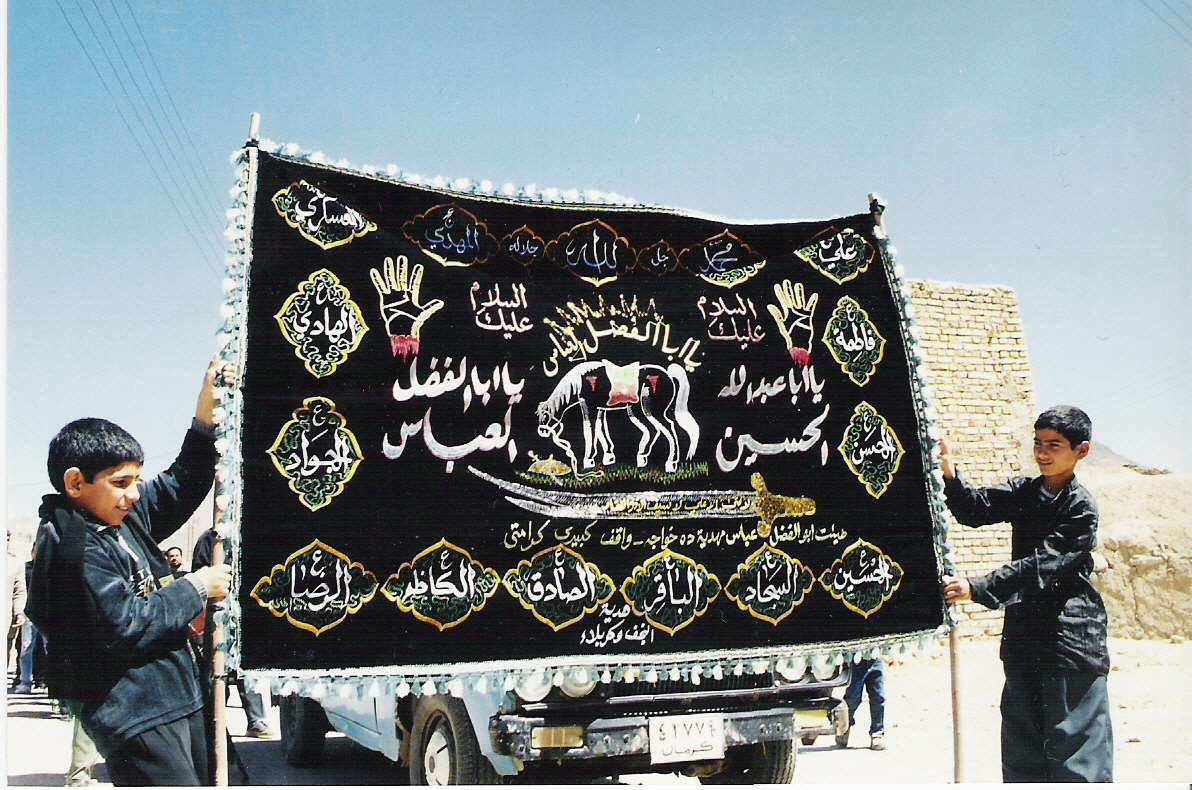
\includegraphics[width=1.97917in,height=1.40972in]{media/image6.jpeg}

\href{https://www.la-croix.com/Religion/Le-Coran-peut-etre-interprete-2021-01-25-1201136852}{Le
Coran peut-il être interprété ?}

Le salafisme, qui représente au moins 40 000 individus, est socialement
dangereux car il impose l'auto-ségrégation, le refus des contacts avec «
ceux qui n'en sont pas ». C'est la raison pour laquelle les spécialistes
des questions de sécurité se refusent à les impliquer dans la lutte
contre le djihadisme. Salafistes et terroristes participeraient à une
même matrice intellectuelle, celle du bien contre le mal, une sorte de
vision sectaire du monde. La différence vient du rapport à la violence :
assumé chez les djihadistes, rejeté chez les salafistes. Leur
fondamentalisme présente l'avantage d'une certaine forme de morale : à
Sartrouville les quartiers salafisés ont vu s'effondrer la toxicomanie
et la délinquance, avec le soutien de la mairie.

\subsection{Confondre l'approche culturelle avec la lutte contre le
terrorisme}

Ces courants ne peuvent être incriminés sur le plan sécuritaire. On
confond donc l'approche culturelle avec la lutte contre le terrorisme. À
moins de changer tout le droit européen, la première doit être menée par
l'éducation, la philosophie, la raison, le débat ; quant à la seconde
elle doit s'appuyer sur le droit et sur des qualifications pénales, et
non sur de vagues impressions de « radicalisation », notion qui n'a
toujours pas été appréhendée de façon rigoureuse en termes sociologiques
et psychologiques.

Comme la guerre d'Algérie nous l'enseigne, une telle manière de
concevoir l'action politique va aboutir à l'effet inverse de celui
recherché : le renforcement de la méfiance collective, le repli
communautaire du côté musulman, l'action violente du côté des « anti »,
et, finalement, la fragmentation sociale et l'insécurité.

\subsection{Islam : les fumées de la radicalisation}

Olivier Hanne, médiéviste (université de Poitiers), chercheur en
islamologie, estime qu'il est très difficile de définir le parcours type
d'une personne radicalisée. Le dernier de trois articles consacrés à
l'islam en France. 
 

Qui parle d'islam aujourd'hui pense aussitôt à la radicalisation. En
2015, on estimait entre 8 000 et 10 000 le nombre de Français
radicalisés. Leurs profils sont si variés qu'il est difficile de donner
des catégories fixes : les mineurs représentent 25 \% des cas, les
femmes 27 \%, les personnes signalées sont plutôt jeunes (entre 16 et 30
ans), leur niveau scolaire est généralement faible, même si l'on
rencontre des diplômés.

La plupart travaillent. Internet représente pour tous ces individus un
passage obligé, même s'il se concrétise différemment : terrain initial
de la radicalisation, facteur de renforcement ou vecteur unique de
l'expression radicale, le partage des contenus djihadistes sur Internet
n'a pas du tout la même fonction chez une adolescente connectée, un
salafiste convaincu et un combattant expérimenté déjà parti en Syrie.

\subsection{Les autorités font feu de tout bois}

De toute évidence, l'attraction pour la radicalité religieuse n'est pas
nécessairement liée à un phénomène de rupture sociale. Les failles de la
société contemporaine (éclatement des familles, déclin des autorités et
des idéologies, chômage, ghettoïsation) créent un terreau facilitateur,
mais nullement déterminant. La frustration individuelle alimente le
recours à des convictions extrêmes, voire le passage à l'acte
terroriste, mais n'est qu'un facteur parmi tant d'autres.

Les autorités font feu de tout bois pour tenter de faire face à une
radicalisation multiforme. En avril 2015, le premier ministre français,
Manuel Valls, annonçait l'ouverture d'une dizaine de centres de
prévention de la radicalisation, dont la plupart furent un échec. Des
sites Internet officiels sont créés et proposent des fiches techniques
contre la radicalisation et le terrorisme, dont le contenu est souvent
simple, voire binaire. Ainsi sur le site
français~\emph{stop-djihadisme.gouv.fr}, un bandeau intitulé «
Radicalisation djihadiste, les premiers signes qui peuvent alerter »
énonce pêle-mêle : « ils se méfient des anciens amis qu'ils considèrent
maintenant comme des impurs » ; « ils changent brutalement leurs
habitudes alimentaires » ; « ils arrêtent d'écouter de la musique car
elle les détourne de leur mission » ; « ils ne regardent plus la
télévision et ne vont plus au cinéma ». Autant de signes extérieurs qui
se rapprochent de l'adolescente anorexique\ldots{} L'efficacité de ces
dispositifs a d'ailleurs été très contestée dès 2015.

\subsection{L'État, tenté d'être omniprésent}

Toute l'entreprise de déradicalisation définit en creux le modèle
positif occidental : monde de loisirs, de consommation, d'épanouissement
personnel et professionnel. Le vocabulaire de la radicalisation masque
le rejet de ce modèle culturel. Et les pouvoirs publics d'hésiter à
appeler leur objectif par son vrai nom : le reconditionnement mental.

Le danger de la déradicalisation se situe dans l'élargissement des
intrusions de l'État : en voulant réinsérer, l'État pénètre dans
l'intimité des individus afin de redéfinir le religieux et lui redonner
une place acceptable. Or, l'État a-t-il compétence pour définir ce
qu'est l'islam, le « bon » islam ? Ne sachant cerner la menace, l'État
est tenté d'être omniprésent, sans en avoir la capacité légale. La
déradicalisation pourrait relever de la posture intellectuelle.

Le problème vient sans doute des hésitations du vocabulaire. Car,
après-tout, qu'est-ce que la radicalisation ? Au
XIX\textsuperscript{e}~le mot anglais~\emph{radical}~était employé pour
désigner les partis politiques britanniques exigeant une réforme
démocratique libérale. Transféré tel quel en France, on l'appliqua aux
partis de gauche, laïques et libéraux qui voulaient réformer la société.

\subsection{Réactions épidermiques}

Le verbe « radicaliser » fut employé régulièrement dans les années
1960-1970 dans une acception politique avec l'idée de « devenir plus
intransigeant, se durcir » ou « plus extrême ». Le premier sens était
donc politique et pas nécessairement négatif. Se déradicaliser était un
synonyme pour « se compromettre ». Appliqué à l'islamisme, le verbe
impose une redéfinition complète des termes : à partir de quand
juge-t-on l'islam intransigeant ou extrême ? par rapport à quelle norme
? à quelle moyenne ?

Les réactions épidermiques qui ont suivi le meurtre de l'enseignant de
Conflans-Sainte-Honorine en octobre 2020 sont tristement révélatrices :
les imams doivent s'exprimer ! les musulmans doivent désavouer le
terrorisme et faire allégeance à la France ! Mais quand ils le font,
c'est encore insuffisant, déloyal et mensonger. Le gouvernement proposa
même qu'ils prient pour la République au cours de la prière collective
du vendredi. Nos références sur la question religieuse restent
tragiquement celles de la Révolution française : comme il y eut les «
prêtres jureurs », adhérant à la loi, contre les « prêtres réfractaires
», obstinés dans leur obéissance à Rome, de la même façon il nous faut
des « imams jureurs », intimement républicains. L'État se retrouve donc
juge des reins et des cœurs.

\bibliography{Theo}
%\bibliographystyle{siam}
%\printbibliography

\listoftheorems[ignoreall,show={Def}]
Les courants contemporains de l’islam Glossaire général

\mn{Vérifier les termes}

bid‘a : innovation ; pratique « déviante ».

da‘wa : invitation ; prédication – appel à la conversion (dans les deux sens).

fasiq : pécheur ; mauvais musulman.

fiqh : compréhension ; corpus du droit musulman.

fitna: discorde, querelle ; conflit interne au monde musulman.

hadith : récit d’un dire ou faire du Prophète, rapporté par ses compagnons.

hajj : pèlerinage annuel à La Mecque.

hijra (héjire) : « exode » - départ de Mahomet pour Médine (622).

‘ibadat : culte ; partie du droit traitant du culte.

ijma‘ : consensus ; consensus des ulama sur un point de droit.

ijtihad : effort ; effort d’interprétation du Coran.

imam : chef suprême de la communauté musulmane ; successeur du Prophète, utilisé communément par les chiites pour Ali et ses descendants.

islah : réforme.

isnad : chaîne ; chaîne de transmission des hadiths.

jihad : lutte ; soit intérieure, contre ses propres faiblesses ; soit extérieure, contre les ennemis de la communauté musulmane.

ka‘aba : monument cubique noir situé au centre de la grande mosquée de La Mecque ; selon les musulmans, désigne l’emplacement du premier autel élevé par Abraham pour le Dieu unique. Point vers lequel se dirigent les musulmans pour prier.

kafir : infidèle, mécréant

khalifa (calife) : successeur, représentant ; successeur du Prophète et chef de la communauté musulmane (sunnisme).

madrasa : école ; lieu où est assuré la transmission du savoir religieux.

mihrab : niche indiquant la direction de La Mecque dans une mosquée.
 
mu‘amalat : relations ; partie du droit traitant des relations humaines.

qibla : orientation de la prière rituelle (salat), correspondant à la direction de La Mecque.

qiyas : raisonnement par analogie (domaine du droit)

salat : prière rituelle.

seyyed : prince, chef ; descendant du Prophète par Hossein ou Hassan, fils d’Ali.

shari‘a : sentier, voie ; loi divine.

sheykh (cheykh) : vieil homme ; chef d’une tribu ; chef religieux ; personne à la tête d’une congrégation soufie, ayant la capacité de guider ses disciples.

shirk : associationnisme : fait d’adorer d’autres êtres en dehors de Dieu.

shura : principe de consultation soufi : mystique musulman sourate : chapitre du Coran
sunna : coutume ; pratiques du Prophète et de la première communauté musulmane, faisant autorité pour guider le mode de vie des croyants et déterminer la loi religieuse.

tafsir : commentaire du Coran.

tajdid : renouveau (=>mujaddidi : qui renouvelle)

taqlid : imitation ; imitation stérile des anciens (par opposition à l’ijtihad).

tariqa : voie : confrérie soufie.

tawhid : unicité (divine). Dogme fondamental de l’islam.

ulama (oulémas) : terme collectif pour désigner les lettrés musulmans.

umma : peuple ou communauté ; communauté islamique dans son ensemble.

waqf : bien immobilier ou foncier dit « de-main-morte », dépendant des institutions religieuses.

zakat : aumône rituelle, obligatoire pour les croyants.

%\listoftheorems


\end{document}